% Autor: Alfredo Sánchez Alberca (asalber@gmail.com)
% !TEX program = xelatex
% ASPECT RATIO FOR YOUTUBE VIDEO
%\documentclass[aspectratio=169,profesionalfont,10pt,svgnames,xcolor=table]{beamer}
% ASPECT RATIO FOR PROJECTOR
% \documentclass[profesionalfont,10pt,svgnames,xcolor=table]{beamer}

% TEMA BEAMER
% \usetheme[progressbar=frametitle,background=light,titleformat=smallcaps,block=fill, numbering=none]{metropolis}

% VERSIÓN ARTÍCULO
% \pdfminorversion=4 % for solving some problems with png graphics in acrobat reader
\documentclass[10pt,a4paper,titlepage]{article}
\usepackage[hyperref]{beamerarticle}

% IDIOMA
\usepackage{polyglossia}
\setdefaultlanguage{spanish}

% FUENTES
\mode<article>{
\usepackage{fontspec}
\setmainfont[Ligatures=TeX]{TeX Gyre Pagella}
\usepackage{unicode-math}
\setmathfont[math-style=ISO,bold-style=ISO]{TeX Gyre Pagella Math}
%\usepackage[sc]{mathpazo}
%\setromanfont[Mapping=tex-text]{Linux Libertine}
%\setsansfont[Mapping=tex-text]{Myriad Pro}
%\setmonofont[Mapping=tex-text]{Courier New}
}
% MEJORA DEL PDF
\mode<article>{\usepackage{microtype}} 

% MATEMÁTICAS
\usepackage{units}

% MÁRGENES
\setbeamersize{text margin left=.5cm, text margin right=.5cm}

% MÁRGENES MODO ARTÍCULO
\mode<article>{\usepackage{fullpage}}
\mode<article>{\usepackage[headsep=1cm, top=3cm, bottom=3cm, left=2.54cm, right=2.54cm]{geometry}}

% COLORES
% Author: Alfredo Sánchez Alberca (asalber@ceu.es)
\usepackage{xcolor}
\definecolor{color1}{RGB}{5,161,230} % Blue
\definecolor{color2}{RGB}{238,50,36} % Red
\definecolor{color3}{RGB}{0,205,0} % Green
\definecolor{color4}{RGB}{243,102,25} % Orange
\definecolor{ocre}{RGB}{243,102,25} % Define the orange color used for highlighting throughout the book
\definecolor{blueceu}{RGB}{5,161,230} % Blue color of CEU logo
\definecolor{greenceu}{RGB}{185,209,16} % Green color of CEU logo
\definecolor{redceu}{RGB}{238,50,36} % Red color of CEU logo
\definecolor{grayceu}{RGB}{111,107,83} % Gray color of CEU logo
\definecolor{coral}{rgb}{1,0.5,0.31} % Orange color for graphics
\definecolor{royalblue1}{rgb}{0.28,0.46,1} % Blue color for graphics
\definecolor{mygreen}{rgb}{0,0.8,0} % Green color for graphics
\definecolor{chaptergrey}{RGB}{5,161,230} % Blue color of CEU logo
\definecolor{DarkBrown}{HTML}{604c38} % Brown of Metropoly theme
\definecolor{DarkTeal}{HTML}{23373b} % Teal of Metropoly theme

% ESTILO DEL ÍNDICE DE CONTENIDOS
\setbeamertemplate{section in toc}[sections numbered]
\setbeamertemplate{subsection in toc}[subsections numbered]

% TABLES
\usepackage{array}
\usepackage{multirow}
\usepackage{colortbl}
\usepackage{booktabs}
\newcommand{\tcrule}{\arrayrulecolor{color1!50!white}\toprule}
\newcommand{\mcrule}{\arrayrulecolor{color1!50!white}\midrule}
\newcommand{\bcrule}{\arrayrulecolor{color1!50!white}\bottomrule}

% GRÁFICOS
\usepackage{pgfplots}
\usepgfplotslibrary{fillbetween}
% ESTILOS PGFPLOTS
% Author: Alfredo Sánchez Alberca (asalber@ceu.es)

\pgfplotsset{colormap={outcolormap}{color=(color1); color=(color1!50)},
             colormap={incolormap}{color=(color2); color=(color2!50)},
             colormap={twocolormap}{color=(color1); color=(color2)}}

% Line styles for plotting 2d functions
\pgfplotscreateplotcyclelist{2dfun cycle}{%
  {color1, line width=0.8pt},
  {color2, line width=0.8pt},
  {color3, line width=0.8pt},
  {color4, line width=0.8pt},
}
% Line and point styles for plotting 2d data
\pgfplotscreateplotcyclelist{2dplot cycle}{%
  {color1, line width=0.8pt, mark=*, mark size=1.5pt},
  {color2, line width=0.8pt, mark=square*, mark size=1.3pt},
  {color3, line width=0.8pt, mark=triangle*, mark size=1.5pt},
  {color4, line width=0.8pt, mark=diamond*, mark size=1.5pt},
}

% Plot styles
\pgfplotsset{
  compat=1.14,
% Basic 2D settings
  2dbaseplot/.style={
    axis line style={<->}, % arrows on the axis
    scale only axis,        % otherwise width won't be as intended: http://tex.stackexchange.com/questions/36297/pgfplots-how-can-i-scale-to-text-width
    x tick label style={font=\small},
    y tick label style={font=\small},
    every axis/.append style={font=\small}, 
  },
% Settings for generic 2D functions 
  gen2dfun/.style={
    2dbaseplot,
    axis x line=middle,
    axis y line=middle,
    xlabel={$x$},         
    ylabel={$y$},          
    every axis x label/.style={at={(ticklabel* cs:1)}, anchor=west,},
	every axis y label/.style={at={(ticklabel* cs:1)}, anchor=south,},
    cycle list name=2dfun cycle,
  },
% Settings for 2D functions 
  2dfun/.style={
    2dbaseplot,
    axis x line=middle,
    axis y line=middle,
    xlabel={$x$},         
    ylabel={$y$},          
    every axis x label/.style={at={(ticklabel* cs:1)}, anchor=west,},
	every axis y label/.style={at={(ticklabel* cs:1)}, anchor=south,},
    x tick label style={font=\tiny},
    y tick label style={font=\tiny},
    cycle list name=2dfun cycle,
  },
% Settings for 2D plots
  2dplot/.style={
    baseplot,
    xmajorgrids=true,
    ymajorgrids=true,
    major grid style={dotted},
    axis x line=bottom,
    axis y line=left,
    legend style={cells={anchor=west}, draw=none, font=\footnotesize},
    x tick label style={font=\tiny}, 
    y tick label style={font=\tiny},
    cycle list name=2dplot cycle,
  },
% Basic 3D settings
  3dbaseplot/.style={
%    axis line style={->}, % arrows on the axis
    scale only axis,        % otherwise width won't be as intended: http://tex.stackexchange.com/questions/36297/pgfplots-how-can-i-scale-to-text-width
    x tick label style={font=\small},
    y tick label style={font=\small},
    z tick label style={font=\small},
    every axis/.append style={font=\small}, 
  },
% Settings for generic 3D functions 
  gen3dfun/.style={
    3dbaseplot,
    xlabel={$x$},         
    ylabel={$y$},
    zlabel={$z$},
    every axis x label/.style={at={(ticklabel cs:0.5)}, anchor=center,},
	every axis y label/.style={at={(ticklabel cs:0.5)}, anchor=center,},
	every axis z label/.style={at={(ticklabel cs:0.5)}, anchor=center,},           
    cycle list name=2dfun cycle,
  },
% Settings for 3D functions 
  3dfun/.style={
    3dbaseplot,
    xlabel={$x$},         
    ylabel={$y$},
    zlabel={$z$},           
    every axis x label/.style={at={(ticklabel cs:0.5)}, anchor=center,},
	every axis y label/.style={at={(ticklabel cs:0.5)}, anchor=center,},
	every axis z label/.style={at={(ticklabel cs:0.5)}, anchor=center,},
	x tick label style={font=\tiny}, 
    y tick label style={font=\tiny},
    z tick label style={font=\tiny},
    cycle list name=2dfun cycle,
  },
}

\usepackage{tikz}
\usetikzlibrary{external, arrows, arrows.meta, calc, shapes, shapes.arrows, positioning, decorations.pathreplacing, intersections, fillbetween, snakes}
\usepackage{tkz-euclide}
\usetkzobj{all}
% CONFIGURACIÓN TIKZ
\tikzset{
	% Transiciones
    invisible/.style={opacity=0},
    visible on/.style={alt={#1{}{invisible}}},
    alt/.code args={<#1>#2#3}{%
      \alt<#1>{\pgfkeysalso{#2}}{\pgfkeysalso{#3}} % \pgfkeysalso doesn't change the path
    },
    % Vectors
    vector/.style={->, color1, thick},
    % Arrow tips
    >=stealth,
  }
% Exportación de gráficos
\mode<article>{
\tikzset{
    png export/.style={
        external/system call={
            xelatex \tikzexternalcheckshellescape -halt-on-error -interaction=batchmode -jobname "\image" "\texsource";
            convert -density 300 -transparent white "\image.pdf" "\image.png"
        }
    }
}
\tikzset{
	svg export/.style={
        external/system call/.add={}%
        {; pdf2svg "\image.pdf" "\image.svg"}
    }
}
\tikzexternalize[prefix=img/exportados/]
\tikzset{png export}
\tikzset{svg export}
}

\usepackage{graphicx}

% ICONOS CREATIVE COMMON
\usepackage[scale=2]{ccicons}

% POSICIÓN DEL LOGO
\setbeamertemplate{title graphic}{
 \vbox to 0pt {
 	\vspace*{0.9\textheight}
 	\inserttitlegraphic
 }
}

% ESPACIO ENTRE PÁRRAFOS
\setlength{\parskip}{0.5em}

% TEOREMAS
\theoremstyle{definition}
\newtheorem{definicion}[theorem]{Definición}
\newtheorem{teorema}[theorem]{Teorema}

% BLOQUES DE COLOR
\setbeamercolor{block title}{
	use=normal text,
	fg=normal text.fg,
	bg=alerted text.fg!50
}


% CABECERAS Y PIÉS 

\mode<article>{
\usepackage{fancyhdr}
\pagestyle{fancy}
\rhead{\sffamily\slshape Manual Básico de Estadística}
\renewcommand{\headrulewidth}{0pt}
%\renewcommand{\floatpagefraction}{.8}
%\renewcommand{\textfraction}{.1} 
} 

% CONFIGURACIÓN EL TÍTULO
% \defbeamertemplate{frametitle}{myframe}{
% 	\nointerlineskip
% 	\begin{beamercolorbox}[wd=\paperwidth,sep=1ex]{frametitle}
% 		\insertframetitle
% 	\end{beamercolorbox}
% } 
% \setbeamertemplate{frametitle}[myframe] 

% COLOR DE SECCIONES MODO ARTÍCULO
\mode<article>{
\usepackage{titlesec}
\titleformat{\section}{\color{color1}\normalfont\Large\bfseries}{\color{color1}\thesection}{1em}{}
\titleformat{\subsection}{\color{color1}\normalfont\large\bfseries}{\color{color1}\thesubsection}{1em}{}
}

% COMANDO PARA RESALTADO
\newcommand{\highlight}[1]{\textcolor{orange}{\textbf{#1}}}

% CONFIGURACIÓN PDF
%\hypersetup{colorlinks=true}


%=====================================================================BODY=====

%---------------------------------------------------------------------cover----
\mode<article>{
\title{\vskip 3cm
\textcolor{color1}{\Huge Manual Básico de Estadística}}
\author{
%Pablo Ares Gastesi (\href{mailto:pablo.aresgastesi@ceu.es}{pablo.aresgastesi@ceu.es}) \and
% José Rojo Montijano (\href{mailto:jrojo.eps@ceu.es}{jrojo.eps@ceu.es}) \and
Alfredo Sánchez Alberca (\href{mailto:asalber@ceu.es}{asalber@ceu.es})
}
\date{Feb 2017\\[1cm]
Departamento de Matemática Aplicada y Estadística\\ CEU San Pablo\\[1cm]

\includegraphics[height=2cm]{img/logo_uspceu}
}
}
\mode<presentation>{
\title{Manual Básico de Estadística}
\author{
%Pablo Ares Gastesi (\href{mailto:pablo.aresgastesi@ceu.es}{pablo.aresgastesi@ceu.es}) \\
Alfredo Sánchez Alberca (\href{mailto:asalber@ceu.es}{asalber@ceu.es})
}
\institute{Departamento de Matemática Aplicada y Estadística\\ CEU San Pablo}
\date{Sep 2017}
\titlegraphic{\hfill
\includegraphics[height=1.5cm]{img/logo_uspceu}}
}


\begin{document}
\mode<article>{\thispagestyle{empty}\maketitle}
\mode<presentation>{\maketitle}

%---------------------------------------------------------------------slide----
\begin{frame}
% Términos de la licencia Creative Commons 4.0
\frametitle{Términos de la licencia \normalsize \ccLogo}%

\scriptsize
Esta obra está bajo una licencia Reconocimiento -- No comercial -- Compartir bajo la misma licencia 2.5 España de Creative Commons.
Para ver una copia de esta licencia, visite \url{http://creativecommons.org/licenses/by-nc-sa/4.0/es/}.

Con esta licencia eres libre de:
\begin{itemize}
\item Copiar, distribuir y mostrar este trabajo.
\item Realizar modificaciones de este trabajo.
\end{itemize}

Bajo las siguientes condiciones:
\begin{center}
\begin{tabular}{cp{0.8\textwidth}}
\ccAttribution & \textbf{Reconocimiento}. Debe reconocer los créditos de la obra de la manera especificada por el autor o el licenciador (pero no de una manera que sugiera que tiene su apoyo o apoyan el uso que hace de su obra).\\ 
\ccNonCommercialEU & \textbf{No comercial}. No puede utilizar esta obra para fines
comerciales.\\ 
\ccShareAlike & \textbf{Compartir bajo la misma licencia}. Si altera o transforma esta obra, o genera una obra derivada, sólo puede distribuir la obra generada bajo una licencia idéntica a ésta.
\end{tabular}
\end{center}

\begin{itemize}
\item Al reutilizar o distribuir la obra, tiene que dejar bien claro los términos de la licencia de esta obra.
\item Estas condiciones pueden no aplicarse si se obtiene el permiso del titular de los derechos de autor.
\item Nada en esta licencia menoscaba o restringe los derechos morales del autor.
\end{itemize}
\end{frame}

\mode<article>{\clearpage}

%---------------------------------------------------------------------slide----
\begin{frame}
\mode<presentation>{\frametitle{Contenidos}}
\setbeamertemplate{section in toc}[sections numbered]
\tableofcontents[hideallsubsections]
\end{frame}

\section{Introducción a la Estadística}

\mode<presentation>{
%---------------------------------------------------------------------slide----
\begin{frame}
\frametitle{Introducción a la Estadística}
\tableofcontents[sectionstyle=show/hide,hideothersubsections]
\end{frame}
}


\subsection{La estadística como herramienta científica}
%---------------------------------------------------------------------slide----
\begin{frame}
\frametitle{¿Qué es la estadística?}
\begin{definicion}[Estadística]
La \emph{estadística} es una rama de las matemáticas que se encarga de la recogida, análisis e interpretación de datos.
\end{definicion}

El papel de la Estadística es extraer información de los datos para adquirir el conocimiento necesario para tomar decisiones.

\begin{center}
\tikzsetnextfilename{introduccion/proposito_estadistica}
\resizebox{\textwidth}{!}{
% Autor: Alfredo Sánchez Alberca (email:asalber@ceu.es)
% Charts that shows the purpose of Statistics
\begin{tikzpicture}[every label/.style={text=color1}]
\tikzstyle{node} = [align=center, node distance=1cm, text=color1]; 
\tikzstyle{arrow} = [-latex, color1, line width=10pt];

\node (data) [label=-90:Datos] at (0,1) {
\includegraphics[height=1.5cm]{img/introduccion/datos.pdf}}; 
\pause
\node (information) [label=-90:Información] at (4.7,1)
{
\includegraphics[height=1.5cm]{img/introduccion/informacion.png}}; 
\node at (2,1) [fill=color1,single arrow,shape border rotate=0,text=white, minimum width=1.1cm]{
\ ESTADÍSTICA\ \phantom{}};
\pause
\node (knowledge) [label=-90:Conocimiento] at (9.5,1) {
\includegraphics[height=1.5cm]{img/introduccion/conocimiento.png}};
\node at (7,1) [fill=color1,single arrow,shape border rotate=0,text=white, minimum width=1.1cm]{
Interpretación\phantom{}};
\pause
\node at (11.5,1) [fill=color1,single arrow,shape border rotate=0,text=white, minimum width=1.1cm]{
\ Decisiones\ \phantom{}};
\end{tikzpicture} 
}
\end{center}

\uncover<5->{
La estadística es imprescindible en cualquier disciplina científica o técnica donde se manejen datos, especialmente si son grandes volúmenes de datos, como por ejemplo en Física, Química, Medicina, Psicología, Economía o Ciencias Sociales.}

\uncover<6->{
\begin{center}
Pero, \alert{\emph{¿por qué es necesaria la Estadística?}}
\end{center}
}
\end{frame}


\note{La Estadística está por todas partes en el mundo que nos rodea y la usamos en multitud de ocasiones en nuestra
vida cotidiana aunque no seamos conscientes de ello. Cuando miramos una factura de la luz, o el gasto del teléfono
móvil, cuando comprobamos la popularidad de nuestros mensajes en las redes sociales, cuando vemos la posición que ocupa
nuestro equipo favorito en la clasificación de la liga, o cuando vemos las predicciones meteorológicas, estamos
usando la Estadística.
Pero formalmente, podríamos definir la Estadística como una rama de las matemáticas que se encarga de la recogida,
análisis e interpretación de datos.

Como tiene que ver con el tratamiento de datos, esto la hace imprescindible en cualquier disciplina científica o
técnica donde se manejen datos, especialmente si son grandes volúmenes de datos, como por ejemplo, la física, la
química, la medicina y las ciencias biosanitarias, pero también en la economía, la psicología o las ciencias sociales.

Pero, en realidad, ¿porqué es necesaria la estadística?
}

%---------------------------------------------------------------------slide----
\begin{frame}
\frametitle{La variabilidad de nuestro mundo}
El científico trata de estudiar el mundo que le rodea; un mundo que está lleno de variaciones que dificultan la
determinación del comportamiento de las cosas.

\begin{center}
\alert{\emph{¡La variabilidad del mundo real es el origen de la estadística!}}
\end{center}

La estadística actúa como disciplina puente entre la realidad del mundo y los modelos matemáticos que tratan de explicarla, proporcionando una metodología para evaluar las discrepancias entre la realidad y los modelos teóricos.

Esto la convierte en una herramienta indispensable en las ciencias aplicadas que requieran el análisis de datos y el diseño de experimentos.
\end{frame}
\note{Bien, podemos decir que los científicos tratamos de estudiar el mundo que nos rodea, para comprenderlo y
controlarlo. Pero vivimos en un mundo con una que está lleno de variaciones que dificultan la determinación del
comportamiento de las cosas. No hay dos personas iguales, ni dos animales iguales, ni dos plantas iguales, ni siquiera
existen dos gotas de agua iguales. Esta enorme biodiversidad, que es la mayor riqueza de nuestro mundo, es al mismo
tiempo el principal obstáculo para comprender los fenómenos naturales.

Así, cuando por ejemplo estamos estudiando una enfermedad y su cura, es posible que un tratamiento funcione con una
persona, pero no sirva a otras, o incluso que deje de funcionar con esa misma persona transcurrido un tiempo, porque la
personas también cambiamos con el tiempo.

Podemos decir, por tanto, que \alert{\emph{¡La variabilidad del mundo real es el origen de la estadística!}}

Así, la Estadística juega un papel clave en el Método Científico, ya que hace de puente entre la realidad del mundo y
los modelos matemáticos que tratan de explicarla, proporcionando una metodología para evaluar las discrepancias entre la
realidad y los modelos teóricos. Y esto la convierte en una herramienta indispensable en las ciencias aplicadas que
requieran el análisis de datos y el diseño de experimentos.
}



\subsection{Población y muestra}
%---------------------------------------------------------------------slide----
\begin{frame}
\frametitle{Población estadística}
\begin{definicion}[Población]
Una \emph{población} es un conjunto de elementos definido por una o más características que tienen todos los elementos, y sólo ellos.
Cada elemento de la población se llama \emph{individuo}.
\end{definicion}

\begin{definicion}[Tamaño poblacional]
El número de individuos de una población se conoce como \emph{tamaño poblacional} y se representa como $N$.
\end{definicion}

A veces, no todos los elementos de la población están accesibles para su estudio.
Entonces se distingue entre:
\begin{description}
\item [Población Teórica:] Conjunto de elementos a los que se quiere extrapolar los resultados del estudio.
\item [Población Estudiada:] Conjunto de elementos realmente accesibles en el estudio.
\end{description}
\end{frame}
\note{A la hora de estudiar un fenómeno natural, lo primero es idenficiar a las unidades experimentales, a las que les
afecta este fenómeno, ya sean seres vivos o no. Así, en el estudio de una enfermedad, las unidades experimentales serían
las personas, pero en un proceso de fabricación de pastillas, las unidades experimentales serían las pastillas.

En Estadística, se llama población al conjunto de elementos definido por una o más características que tienen todos los
elementos, y sólo ellos. Y a cada elemento de la población se llama \emph{individuo}, aunque un individuo no
necesariamente tiene que ser una persona, sino que puede ser cualquier objeto.

Por otro lado, el número de individuos de una población se conoce como \emph{tamaño poblacional} y lo representaremos
con la letra $N$ mayúscula.

Por ejemplo, en unas elecciones generales a la presidencia del gobierno, la población serían todos los individuos del
estado con derecho a voto. En el estudio de una enfermedad, la población sería todas las personas que
tienen la enfermedad. Y en un proceso de control de calidad en la fabricación de un fármaco,  la población estaría
formada por todos los fármacos que se producen en la fábrica.

A veces, no todos los elementos de la población están accesibles para su estudio. Entonces se distingue entre:
\begin{description}
\item [Población Teórica:] Conjunto de elementos a los que se quiere extrapolar los resultados del estudio.
\item [Población Estudiada:] Conjunto de elementos realmente accesibles en el estudio.
\end{description}

Por ejemplo, en el caso del estudio de una enfermedad, la población teórica sería todas las personas que contraigan la
enfermedad, incluso si aún no han nacido, mientras que la población estudiada se limitaría al número de personas
enfermas que realmente podemos estudiar (obsérvese que incluso quedarían fuera las personas enfermas actualmente que no
supieran que lo están o a las que no pudiésemos acceder físicamente para estudiarlas.)
}


%---------------------------------------------------------------------slide----
\begin{frame}
\frametitle{Inconvenientes en el estudio de la población}
El científico estudia un determinado fenómeno en una población para comprenderlo, obtener conocimiento sobre el mismo, y así poder controlarlo.

Pero, para tener un conocimiento completo de la población es necesario estudiar todos los individuos de la misma.

Sin embargo, esto no siempre es posible por distintos motivos:
\begin{itemize}
\item El tamaño de la población es infinito, o bien es finito pero demasiado grande.
\item Las pruebas a que se someten los individuos son destructivas.
\item El coste, tanto de dinero como de tiempo, que supondría estudiar a todos los individuos es excesivo.
\end{itemize}
\end{frame}
\note{Como hemos dicho, el científico suele estudiar un determinado fenómeno en una población para comprenderlo,
obtener conocimiento sobre el mismo, y así poder controlarlo.

Pero, para tener un conocimiento completo de la población \emph{es necesario estudiar todos los individuos de la misma}.

Sin embargo, esto no siempre es posible por distintos motivos:
\begin{itemize}
\item En primer lugar, el tamaño de la población suele ser pero demasiado grande para poder estudiar uno por uno a todos
los individuos. A veces incluso podemos tener poblaciones de tamaño infinito, como por ejemplo en el estudio de una
enfermeda, ya que también formarían parte de la población las personas que aún no han nacido pero que acaben
desarrollándola.
\item Otras veces, las pruebas a que se someten los individuos para su estudio son destructivas. Por ejemplo en un
proceso de control de calidad en la fabriación de un fármaco, el fármaco suele someterse a pruebas que lo alteran, por
lo que ya no se podría comercializar. En este caso, un estudio completo de la población, acabaría con la población y no
podríamos vender ni un sólo fármaco.
\item Finalmente, a veces el problema es simplemente una cuestión de que el coste, tanto de dinero como de
tiempo, que supondría estudiar a todos los individuos es excesivo.
\end{itemize}

En cualquier caso, es raro que podamos estudiar a todos los individuos de una población para tener un conocimiento
completo de la misma.
}

%---------------------------------------------------------------------slide----
\begin{frame}
\frametitle{Muestra estadística}
Cuando no es posible o conveniente estudiar todos los individuos de la población, se estudia sólo una parte de la misma.

\begin{definicion}[Muestra]
Una \emph{muestra} es un subconjunto de la población.
\end{definicion}

\begin{definicion}[Tamaño muestral]
Al número de individuos que componen la muestra se le llama \emph{tamaño muestral} y se representa por $n$.
\end{definicion}

Habitualmente, el estudio de una población se realiza a partir de muestras extraídas de dicha población.

Generalmente, el estudio de la muestra sólo aporta conocimiento aproximado de la población. Pero en muchos casos es \emph{suficiente}.
\end{frame}
\note{
Así pues, cuando no es posible o conveniente estudiar todos los individuos de la población, no queda más remedio que
estudiar sólo una parte de la misma. Esta pequeña parte de la población que se estudia se conoce como muestra.

En Estadística, se llama muestra a cualquier subconjunto de la población, y al número de individuos que componen la
muestra se le llama tamaño muestral y lo representaremos por $n$ minúscula, para distinguirlo del tamaño de la población
que habíamos representado con N mayúscula.

Habitualmente, el estudio de una población se realiza a partir de muestras extraídas de dicha población, pero debemos
ser conscientes que el estudio de las muestra sólo aporta un conocimiento aproximado de la población. Es decir, nunca
vamos a tener un conocimiento completo de la población a partir de las muestras, sin embargo, si la muestra es lo
suficientemente grande y representativa de la población, podremos lograr tener un conocimiento de la población
suficiente, para comprender el fenómeno e incluso tomar decisiones sin asumir demasiados riesgos.
}


%---------------------------------------------------------------------slide----
\begin{frame}
\frametitle{Determinación del tamaño muestral}
Una de las preguntas más interesantes que surge inmediatamente es:
\begin{center}
\alert{\emph{¿cuántos individuos es necesario tomar en la muestra para tener un conocimiento aproximado pero suficiente de la población?}}
\end{center}

La respuesta depende de varios factores, como la variabilidad de la población o la fiabilidad deseada para las extrapolaciones que se hagan hacia la población.

Por desgracia no se podrá responder hasta casi el final del curso, pero en general, cuantos más individuos haya en la muestra, más fiables serán las conclusiones sobre la población, pero
también será más lento y costoso el estudio.
\end{frame}
\note{En el momento de tomar una muestra para estudiar una población, una de las preguntas que surge de manera inmediata
es:
\emph{¿cuántos individuos es necesario tomar en la muestra para tener un conocimiento aproximado pero suficiente de la
población?}

La respuesta no es sencilla, y depende de varios factores, como puede ser la variabilidad de la población o cómo de
preciso o aproximado queremos que sea nuestro conocimiento de la población. Parece lógico pensar que en una población
con gran variabilidad habrá que estudiar más individuos que en una población con poca variabilidad para tener un
conocimiento aproximado de esta. Del mismo modo, si queremos un conocimiento muy aproximado a la realidad, tendremos que
estudiar más individuos que si no necesitamos un conocimiento tan preciso.

En general, cuantos más individuos haya en la muestra, más preciso sera nuestro conocimiento de la población y más
fiables serán las conclusiones sobre esta, pero también será más lento y costoso el estudio. Así pues, antes de comenzar
cualquier estudio de una población debemos plantearnos siempre estas preguntas y determinar el tamaño muestral
necesario, y no más, para tener un conocimiento suficiente de la población.

Por desgracia no podremos responder de manera operativa a esta pregunta este curso, ya que se requieren conocimientos
avanzados que se verán en la segunda parte del curso.
}


%---------------------------------------------------------------------slide----
\begin{frame}
\frametitle{Determinación del tamaño muestral}
\framesubtitle{Muestra pequeña de los píxeles de una imagen}
\mode<article>{\textbf{Example}. Para entender a qué nos referimos cuando hablamos de un tamaño muestral suficiente para comprender lo que ocurre en la población, podemos utilizar el siguiente símil en que se trata de comprender el motivo que representa una fotografía.

Una fotografía digital está formada por multitud de pequeños puntitos llamados píxeles que se dispone en una enorme tabla de filas y columnas (cuantas más filas y columnas haya se habla de que la foto tiene más resolución).
Aquí la población estaría formada por todos y cada uno de los píxeles que forman la foto.
Por otro lado cada pixel tiene un color y es la variedad de colores a lo largo de los pixels la que permite formar la imagen de la fotografía.

\begin{center}
\emph{¿Cuántos píxeles debemos tomar en una muestra para averiguar la imagen de la foto?}
\end{center}

La respuesta depende de la variabilidad de colores en la foto.
Si todos los píxeles de la foto son del mismo color, entonces un sólo pixel basta para desvelar la imagen.
Pero, si la foto tiene mucha variabilidad de colores, necesitaremos muchos más píxeles en la muestra para descubrir el motivo de la foto.
}
¿Puedes averiguar el motivo de la foto?
\begin{center}
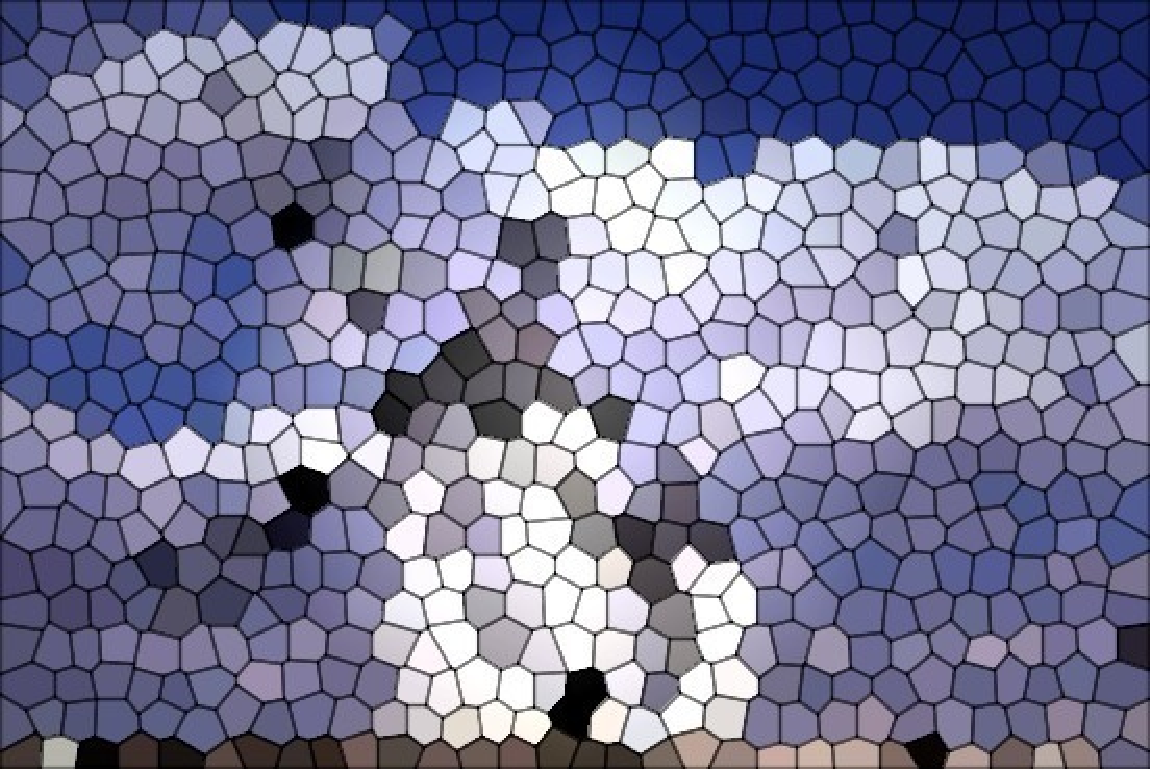
\includegraphics[scale=0.45]{img/introduccion/muestra_molino1}

\emph{¡Con una muestra pequeña es difícil averiguar el contenido de la imagen!}
\end{center}
\end{frame}
\note{Para entender a qué nos referimos cuando hablamos de un tamaño muestral suficiente para comprender lo que ocurre
en la población, podemos utilizar el siguiente símil en que se trata de comprender el motivo que representa una
fotografía.

Como sabéis, una fotografía digital está formada por multitud de pequeños puntitos llamados píxeles que se dispone
en una enorme tabla de filas y columnas (cuantas más filas y columnas haya se habla de que la foto tiene más
resolución). Aquí la población estaría formada por todos y cada uno de los píxeles que forman la foto. Por otro lado cada
pixel tiene un color y es la variedad de colores a lo largo de los pixels la que permite formar la imagen de la
fotografía.

Supongamos que queremos comprender el motivo de la fotografía y para ello tomamos sólo una pequeña muestra de los píxeles
de ella, como esta que aparece en la pantalla. ¿Serías capaz de averiguar de qué se trata?

Seguramente no has podido averiguar el motivo de la fotografía, porque en este caso el número de píxeles que hemos tomado
en la muestra es insuficiente para comprender toda la variabilidad de colores que hay en la foto.
}


%---------------------------------------------------------------------slide----
\begin{frame}
\frametitle{Determinación del tamaño muestral}
\framesubtitle{Muestra mayor de los píxeles de una imagen}
\mode<article>{Seguramente no has podido averiguar el motivo de la fotografía, porque en este caso el número de píxeles que hemos tomado en la muestra es insuficiente para comprender toda la variabilidad de colores que hay en la foto.

La siguiente imagen contiene una muestra mayor de píxeles.}
\begin{center}
¿Eres capaz de adivinar el motivo de la foto ahora?

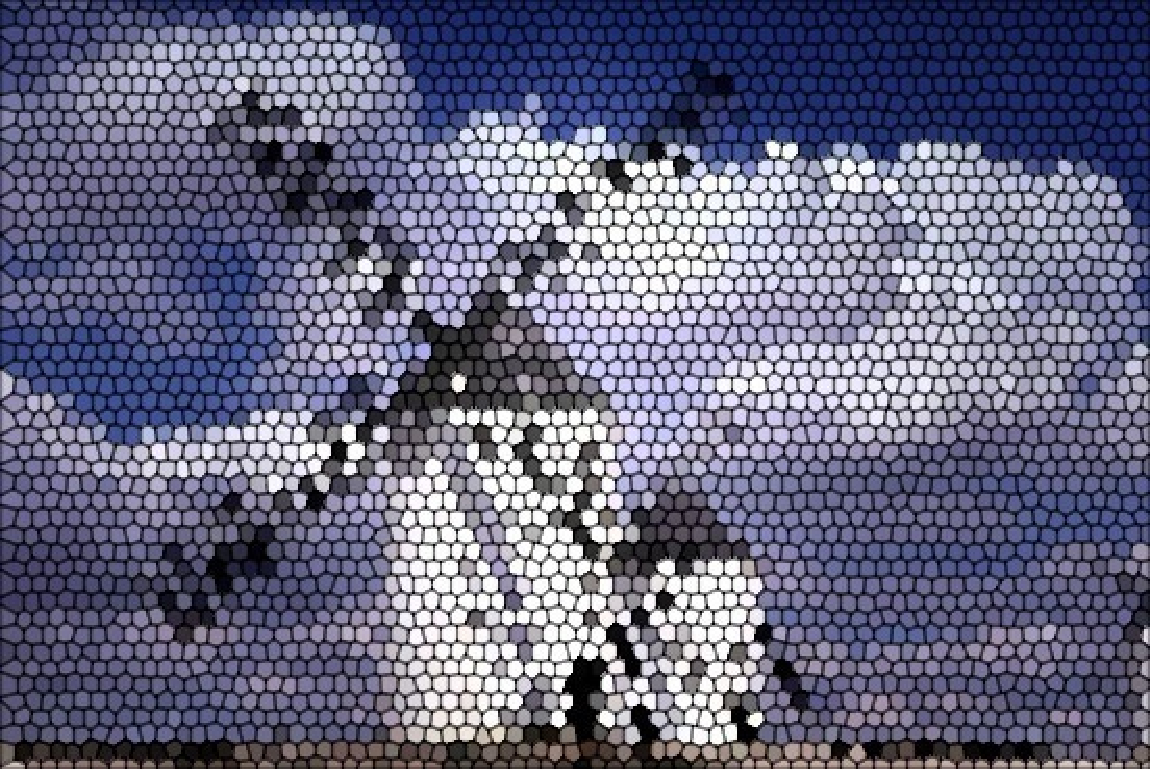
\includegraphics[scale=0.45]{img/introduccion/muestra_molino2}

\emph{¡Con una muestra mayor es más fácil averiguar el contenido de la imagen!}
\end{center}
\end{frame}
\note{Sin embargo, si tomamos una muestra mayor, como esta otra, seguramente que ya si sabrías decir cuál es la imagen
de la foto. ¿Eres capaz?
}


%---------------------------------------------------------------------slide----
\begin{frame}
\frametitle{Determinación del tamaño muestral}
\framesubtitle{Población completa de los píxeles de una imagen}
\begin{center}
Y aquí está la población completa

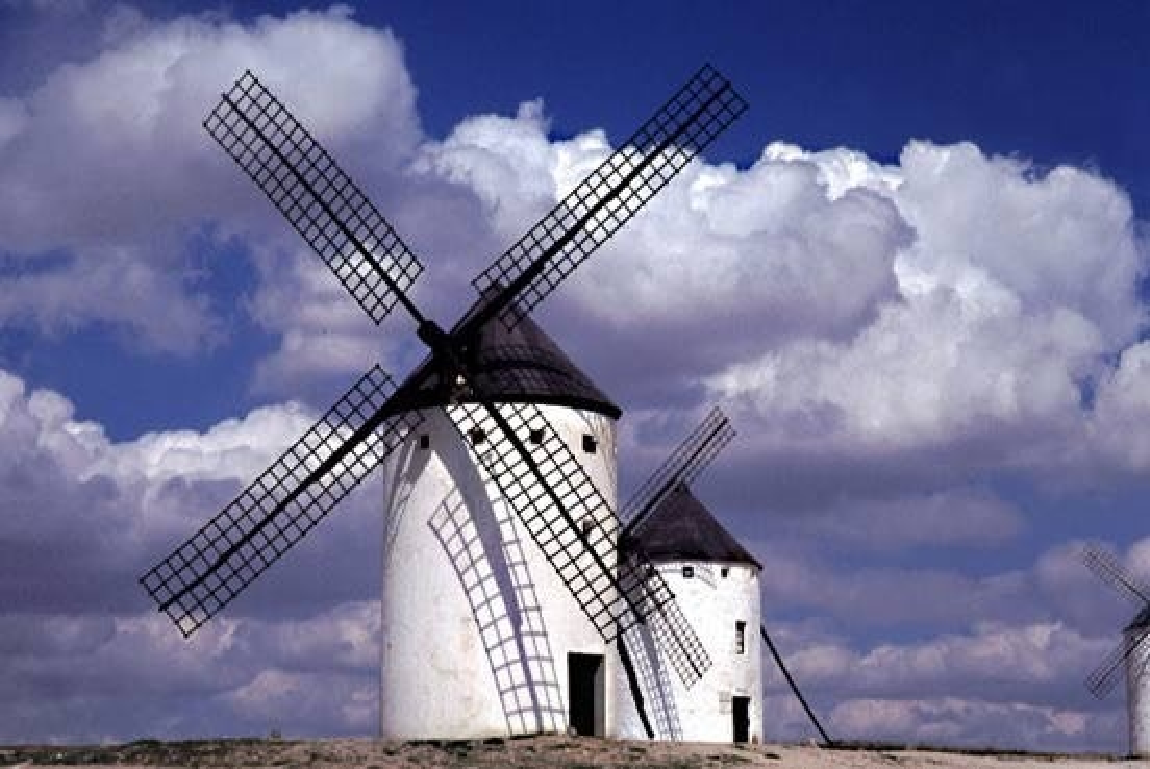
\includegraphics[scale=0.45]{img/introduccion/muestra_molino3}

\emph{¡No es necesario conocer todos los píxeles para averiguar la imagen!}
\end{center}
\end{frame}
\note{
Efectivamente, se trata de unos molinos de viento, y si has sido capaz de averiguarlo es porque en la segunda muestra el número de píxeles tomados en la muestra era suficiente para comprender el motivo de la fotografía.

Evidentemente, cuanto mayor sea la variabilidad de colores de la fotografía, mayor será el tamaño muestral requerido
para comprender el motivo de la foto, y cuanto menos variabilidad de colores haya en la foto, menos pixels habrá que
tomar, hasta el punto de que en una foto donde no hubiese variabilidad de colores, es decir, donde todos los pixels
tuviesen el mismo color, bastaría con tomar un pixel para conocer el motivo de la foto.

Bien, pues esto mismo pasa en las poblaciones que estudiaremos en el ámbito de las Ciencias de la Salud.
}

%---------------------------------------------------------------------slide----
\begin{frame}
\frametitle{Tipos de razonamiento}

\begin{center}
\tikzsetnextfilename{introduccion/tipos_razonamiento}
\resizebox{0.5\textwidth}{!}{% Autor: Alfredo Sánchez Alberca (email:asalber@ceu.es)
\begin{tikzpicture}[every label/.style={text=color1}]
\tikzstyle{node} = [align=center, node distance=1cm]; 
\tikzstyle{arrow} = [-latex, color1, line width=10pt];

\node (population) [label=90:Población] at (0,5) {
\includegraphics[height=2cm]{img/introduccion/poblacion.pdf}}; 
\node (sample) [label=-90:Muestra] at (0,0) {
\includegraphics[height=2cm]{img/introduccion/muestra.png}};
\node at (-0.5,2.6) [fill=color1,single arrow,shape border rotate=270,text=white, minimum width=1.2cm]{
\rotatebox{90}{Deducción}\phantom{}};
\node[node] at (-2,2.5) {De lo general\\ a lo particular};
\pause
\node at (0.5,2.4) [fill=color1,single arrow,shape border rotate=90,text=white, minimum width=1.2cm]{
\rotatebox{-90}{Inducción}\phantom{}};
\node[node] at (2.1,2.5) {De lo particular\\ a lo general};
\end{tikzpicture} }
\end{center}
\end{frame}
\note{Como se ha dicho antes, habitualmente realizaremos el estudio de la población a partir de muestras y luego
trataremos de extrapolar lo observado en la muestra al resto de la población. A este tipo de razonamiento que saca
conclusiones desde la muestra hacia la población se le conoce como razonamiento inductivo.

A diferencia del razonamiento deductivo que va de lo general a lo particular, o en nuestro caso de la población a la
muestra, el razonamiento inductivo no garantiza la certeza de las conclusiones, por lo que debemos ser cuidadosos a la
hora de generalizar sobre la población lo observado en al muestra, ya que si no se hacen bien las cosas podrían
cometerse errores.

Seguramente muchos habréis oído hablar de aquel científico loco que no sabía porqué la gente se emborrachaba y decidió
experimentar. Un día probó whisky con leche, y se emborrachó, otro día probó ron con leche y se emborrachó, y otro día
probó ginebra con leche y también se emborrachó. ¿Sabéis cuál es la conclusión a la que llegó? Efectivamente, concluyó
en su estudio que la causa de la embriaguez era la leche.

En este caso, el científico loco aplicó bien el método inductivo, sin embargo, las conclusiones fueron falsas porque no
hico un buen diseño del experimento y porque la muestra de bebidas tomadas no era representativa. Si hubiese mezclado la
leche con agua, habría visto enseguida que la leche no era la causa de su embriaguez.

Esto mismo podría ocurrir en nuestros estudios, si no tenemos cuidado a la hora de diseñar el experimento, y sobre todo,
si no tomamos una muestra representativa de la población. Cuando hablamos de que una muestra sea representativa, nos
referimos a que refleje las mismas características de la población de la que se ha tomado, pero a pequeña escala. Más
adelante veremos cómo debemos tomar la muestra para garantizar su representatividad.
}


%---------------------------------------------------------------------slide----
\begin{frame}
\frametitle{Tipos de razonamiento}
\begin{description}
\item [Características de la deducción:] Si las premisas son ciertas, garantiza la certeza de las conclusiones (es decir, si algo se cumple en la población, también se cumple en la muestra). Sin embargo, \alert{\emph{¡no aporta conocimiento nuevo!}}
\item [Características de la inducción:] No garantiza la certeza de las conclusiones (si algo se cumple en la muestra, puede que no se cumpla en la población, así que ¡cuidado con las extrapolaciones!).
Sin embargo, \alert{\emph{¡es la única forma de generar conocimiento nuevo!}}
\end{description}

La estadística se apoya fundamentalmente en el razonamiento inductivo ya que utiliza la información obtenida a partir de muestras para sacar conclusiones sobre las poblaciones.
\end{frame}


\subsection{Muestreo}
%---------------------------------------------------------------------slide----
\begin{frame}
\frametitle{Muestreo}
\begin{definicion}[Muestreo]
El proceso de selección de los elementos que compondrán una muestra se conoce como \emph{muestreo}.
\end{definicion}
\begin{center}
\tikzsetnextfilename{introduccion/muestreo}
\resizebox{0.8\textwidth}{!}{% Autor: Alfredo Sánchez Alberca (email:asalber@ceu.es)
\begin{tikzpicture}[every label/.style={text=color1}]
\tikzstyle{node} = [align=center, node distance=1cm]; 
\tikzstyle{arrow} = [-latex, color1, line width=12pt];

\node (population) [label=-90:Población] at (0,0) {
\includegraphics[height=2cm]{img/introduccion/poblacion.pdf}}; 
\node (sample) [label=-90:Muestra] at (6,0) {
\includegraphics[height=2cm]{img/introduccion/muestra.png}};
\node at (3.3,0) [fill=color1,single arrow,shape border rotate=0,text=white, minimum width=1.2cm]{
\ Muestreo\ \phantom{}};
\end{tikzpicture} }
\end{center}
Para que una muestra refleje información fidedigna sobre la población global debe ser representativa de la misma, lo que significa que debe reproducir a pequeña escala la variabilidad de la población.

\begin{center}
\alert{\emph{El objetivo es obtener una muestra representativa de la población.}}
\end{center}
\end{frame}
\note{En Estadística, al proceso por el cual se seleccionan a los individuos de la muestra se le llama muestreo.

Y como hemos visto antes, es muy importante que la muestra sea representativa de la población para que podamos sacar
conclusiones fiables sobre la población.
}


%---------------------------------------------------------------------slide----
\begin{frame}
\frametitle{Modalidades de muestreo}
Existen muchas técnicas de muestreo pero se pueden agrupar en dos categorías:
\begin{description}
\item[Muestreo Aleatorio] Elección aleatoria de los individuos de la muestra.
Todos tienen la misma probabilidad de ser elegidos (\emph{equiprobabilidad}).
\item[Muestreo No Aleatorio:] Los individuos se eligen de forma no aleatoria.
Algunos individuos tienen más probabilidad de ser seleccionados que otros.
\end{description}
Sólo las técnicas aleatorias evitan el sesgo de selección, y por tanto,  garantizan la representatividad de la muestra extraída, y en consecuencia la validez de las conclusiones.

Las técnicas no aleatorias no sirven para hacer generalizaciones, ya que no garantizan la representatividad de la muestra.
Sin embargo, son menos costosas y pueden utilizarse en estudios exploratorios.
\end{frame}
\note{En general, existen puchos procedimientos para seleccionar a los individuos de la muestra, pero se suelen dividir
en dos tipos:
\begin{description}
\item[Muestreo Aleatorio] Que se caracteriza por la elección aleatoria de los individuos de la muestra. Es decir los
individuos se eligen al azar, lo cual quiere decir que todos los individuos de la población tienen la misma probabilidad
de ser elegidos en la muestra.
\item[Muestreo No Aleatorio:] Que es cuando los individuos se eligen de forma no aleatoria.
\end{description}

Bien, debemos tener presente que sólo las técnicas aleatorias evitan el sesgo de selección, y por tanto, garantizan
la representatividad de la muestra extraída, y en consecuencia la validez de la inferencia que hagamos sobre la
población. Por tanto siempre que queramos sacar conclusiones fiables sobre la población debemos utilizar muestreos
aleatorios.

Las técnicas no aleatorias no sirven para hacer generalizaciones, ya que no garantizan la representatividad de la muestra.
Sin embargo, son menos costosas y pueden utilizarse en estudios exploratorios. En muchos estudios no tendremos
capacidad para hacer una elección aleatoria de los individudos de la muestra y nos tendremos que conformar con una
muestra dada. En estos casos no deberíamos hacer generalizaciones sobre la población y deberíamos ser muy cautelosos a
la hora de sacar conclusiones sobre esta.
}


%---------------------------------------------------------------------slide----
\begin{frame}
\frametitle{Muestreo aleatorio simple}
Dentro de las modalidades de muestreo aleatorio, el tipo más conocido es el \emph{muestreo aleatorio simple}, caracterizado por:
\begin{itemize}
\item Todos los individuos de la población tienen la misma probabilidad de ser elegidos para la muestra.
\item La selección de individuos es con reemplazamiento, es decir, cada individuo seleccionado es devuelto a la población antes de seleccionar al siguiente (y por tanto no se altera la población de partida).
\item Las sucesivas selecciones de un individuo son independientes.
\end{itemize}
La única forma de realizar un muestreo aleatorio es asignar un número a cada individuo de la población (\emph{censo}) y realizar un sorteo aleatorio.
\end{frame}
\note{La técnica de muestreo aleatorio más conocida es el muestreo aleatorio simple, que se caracteriza por tres
propiedades:
\begin{itemize}
\item Todos los individuos de la población tienen la misma probabilidad de ser elegidos para la muestra. Si no no sería
aleatorio.
\item La selección de individuos es con reemplazamiento, es decir, tras seleccionar a un individuo se devuelve a la
población antes de realizar la siguiente elección. Esto tiene el riesgo de incluir al mismo individuo varias veces en
la muestra, aunque en la práctica, con poblacione grandes es casi imposible, pero a cambio se consigue que no se altere
la población de partida.
\item Las sucesivas selecciones de un individuo son independientes, y por tanto la elección de un determinado individuo
no influye en la elección o no de otros.
\end{itemize}

En general, existen bastantes dudas en la comunidad científica sobre lo que es un muestreo aleatorio y lo que no lo es.
Por ejemplo, mucha gente piensa que hacer una encuesta a pie de calle es un muestreo aleatorio, pero en realidad no lo
es porque no todas las personas de la población tienen las misma probabilidad de ser encuestadas (hay gente que ni
siquiera sale a la calle). La única manera de garantizar que un muestreo es aleatorio es disponiendo de un censo de la
población de manera que todos y cada uno de los individuos tengan un número identificativo único y realizando un sorteo,
como el de la lotería, para extraer los identificadores de los individuos que formarán parte de la muestra. Este sorteo
se suele hacer habitualmente mediante algún programa informático que genere números de forma aleatoria.
}


\subsection{Variables estadísticas}

%---------------------------------------------------------------------slide----
\begin{frame}
\frametitle{Variables estadísticas y datos}
Todo estudio estadístico comienza por la identificación de las características que interesa estudiar en la población y que se medirán en los individuos de la muestra.
\begin{definition}[Variable estadística]
Una \emph{variable estadística} es una propiedad o característica medida en los individuos de la población.

Los \emph{datos} son los valores observados en las variables estadísticas.
\end{definition}

\begin{center}
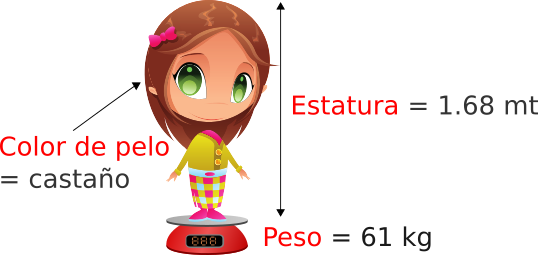
\includegraphics[scale=0.5]{img/introduccion/variables_estadisticas.png}
\end{center}
\end{frame}


%---------------------------------------------------------------------slide----
\begin{frame}
\frametitle{Variables estadísticas y atributos}
De acuerdo a la naturaleza de los valores y su escala, se tiene:
\begin{itemize}
\item \highlight{Variables cualitativas o atributos:} Miden cualidades no numéricas.
Pueden ser:
\begin{itemize}
\item \highlight{Nominales:} No existe un orden natural entre las categorías.\\
Ejemplo: El color de pelo o el sexo.
\item \highlight{Ordinales:} Existe un orden natural entre las categorías.\\
Ejemplo: El nivel de estudios o la gravedad de una enfermedad.
\end{itemize}
\item \highlight{Variables cuantitativas:} Miden cantidades numéricas.
Pueden ser:
\begin{itemize}
\item \highlight{Discretas:} Toman valores numéricos aislados (habitualmente números enteros).\\
Ejemplo: El número de hijos o de coches en una familia.
\item \highlight{Continuas:} Pueden tomar cualquier valor en un intervalo real.\\
Ejemplo: La estatura, el peso, o la edad de una persona.
\end{itemize}
\end{itemize}
\note{Todo estudio estadístico comienza por la identificación de las características que interesa estudiar en la
población y que se medirán en los individuos de la muestra. Estas características pueden ser de dos tipos según sean de
naturaleza cuantitativa o cualitativa, es decir, si miden cantidades o cualidades. Las características de naturaleza
cualitativa se conocen como atributos o variables cualitativas, mientras que las de naturaleza cuantitativas se conocen
como variables estadísticas o cuantitativas.

Los atributos, a su vez, pueden ser de dos tipos, nominales, cuando no existe un orden natural entre las modalidades o
valores que puede tomar el atributo, como por ejemplo el color de ojos, que puede ser negro, azul, verde, etc. pero no
tiene sentido ordenar los colores; u ordinales, cuando existe un orden natural entre las modalidades, como por ejemplo
el grado de gravedad de un paciente que puede ir de leve, moderado, grave o muy grave siguiendo un orden de menor a
mayor gravedad.

Por su parte las variables estadísticas también pueden clasificarse como discretas, cuando toman valores aislados que
suelen ser números enteros, como por ejemplo el número de hijos de una familia, que puede ser 0, 1, 2, 3, es decir, un
número entero posito pero no puede tomar valores decimales como 1.27; o continuas cuando si pueden tomar cualquier
valor dentro de un intervalo real, como por ejemplo la estatura, donde, entre dos estaturas cualesquiera como 1.60 y
1.70 podemos encontrar infinitas estaturas posibles.

Conocer el tipo de las variables u atributos es fundamental pues las técnicas que se utilizarán
para describirlas dependen del tipo de característica.

A la hora de seleccionar las variables que se estudiarán conviene tomar todas las variables que puedan tener relación
con el fenómeno que se pretende estudiar, y en esto cabe más pecar por exceso que por defecto, ya que si con el
trascurso del estudio se observa que una variable no aporta nada, siempre se puede descartar a posteriori, mientras que
si se observa que falta una variable importante, en la mayoría de los casos no se podrá volver atrás para
medirla.

En el caso de las variables numéricas, es importante también explicitar las unidades en que van a medirse.
}
\end{frame}

%---------------------------------------------------------------------slide----
\begin{frame}
\frametitle{Tipos de variables estadísticas}
\begin{center}
\tikzsetnextfilename{introduccion/tipos_variables}
\resizebox{\textwidth}{!}{% Author: Alfredo Sánchez Alberca (email:asalber@ceu.es)
% Types of statistical variables
\tikzset{every node/.style = {align=center, inner sep=2pt, text centered}}
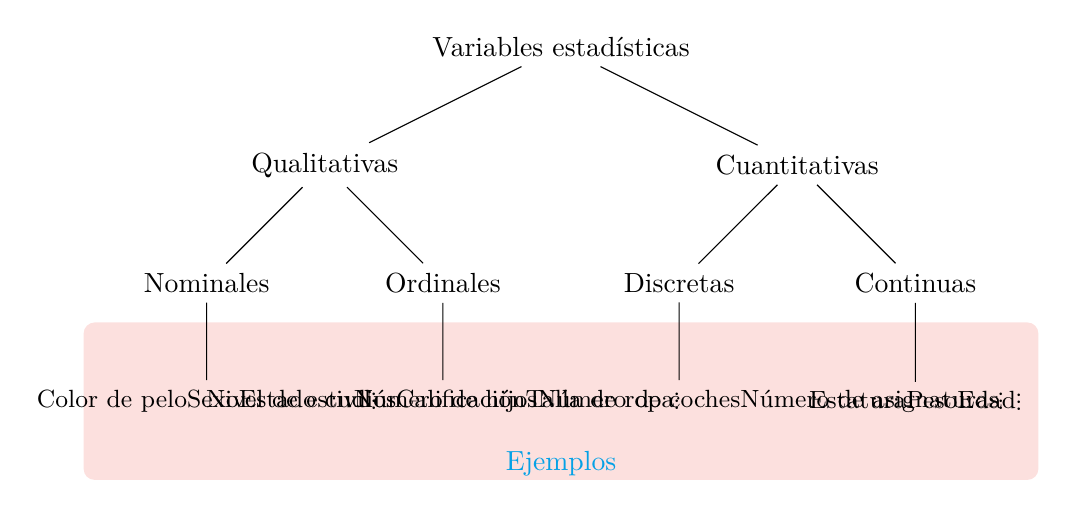
\begin{tikzpicture}[-, >=stealth', level distance = 1.5cm,
	level 1/.style={sibling distance = 6cm},
	level 2/.style={sibling distance = 3cm},
	level 3/.style={font=\small}
] 

\node [rectangle, minimum height=2cm, minimum width=\textwidth, fill=color2!30, rounded corners, opacity=0.5] at
(0,-4.5) {\phantom{0}}; 

\node {Variables estadísticas}
	child{node{Qualitativas}
		child{node{Nominales}
			child{node{Color de pelo\\ Sexo\\ Estado civil\\ $\vdots$}}
		}     
       	child{node{Ordinales}
			child{node{Nivel de estudios\\ Calificación\\ Talla de ropa\\ $\vdots$}}
		}           
    }
	child{node{Cuantitativas}
		child{node{Discretas}
			child{node{Número de hijos\\ Número de coches\\ Número de asignaturas\\ $\vdots$}}
		}     
        child{node{Continuas}
			child{node{Estatura\\ Peso\\ Edad\\ $\vdots$}}
%           	child{node{\parbox[top][1cm][t]{2cm}{Interval}}}
%            child{node{\parbox[top][1cm][t]{2cm}{Ratio}}}
        }               
    }
; 

\node [text=color1] at (0,-5.3) {Ejemplos};
\end{tikzpicture}}
\end{center}
\end{frame}



%---------------------------------------------------------------------slide----
\begin{frame}
\frametitle{Tipos de variables estadísticas}
\framesubtitle{Eligiendo la variable adecuada}
En ocasiones una característica puede medirse mediante variables de distinto tipo.

\textbf{Ejemplo} Si una persona fuma o no podría medirse de diferentes formas:
\begin{itemize}
\item Fuma: si/no. (Nominal)
\item Nivel de fumador: No fuma / ocasional / moderado / bastante / empedernido. (Ordinal)
\item Número de cigarros diarios: 0,1,2,\ldots (Discreta)
\end{itemize}

En estos casos es preferible usar variables cuantitativas a cualitativas.
Dentro de las cuantitativas es preferible usar las continuas a las discretas y dentro de las cualitativas es preferible usar ordinales a nominales pues aportan más información.

\begin{center}
\tikzsetnextfilename{introduccion/informacion_variables}
\scalebox{1}{% Author: Alfredo Sánchez Alberca (email:asalber@ceu.es)
% Plot with the level of information of each variable type

\begin{tikzpicture}[scale=0.5]
\tikzstyle{node} = [align=center, text=color1];
\useasboundingbox (-0.5,-0.5) rectangle (18.5,2.7);
\draw[stealth-stealth, thin, color1!90, line width=12pt] (-0.5,1.5) -- (18.5,1.5);
\node at (1.5,1.5) {\color{white}-- Info};
\node at (16.5,1.5) {\color{white} + Info};
\node[node] at (1,0) {Nominales};
\node[node] at (5,0) {Ordinales};
\node[node] at (9,0) {Discretas};
\node[node] at (13,0) {Intervalo};
\node[node] at (17,0) {Ratio};
\end{tikzpicture}}
\end{center}
\end{frame}


%---------------------------------------------------------------------slide----
\begin{frame}
\frametitle{Tipos de variables estadísticas}
De acuerdo al papel que juegan en el estudio:
\begin{itemize}
\item \highlight{Variables independientes:} Variables que supuestamente no dependen de otras variables en el estudio.
Habitualmente son las variables manipuladas en el experimento para ver su efecto en las variables dependientes.
Se conocen también como \emph{variables predictivas}.
\item \highlight{Variables dependientes:} Variables que supuestamente dependen de otras variables en el estudio.
No son manipuladas en el experimento y también se conocen como \emph{variables respuesta}.
\end{itemize}

\textbf{Ejemplo} En un estudio sobre el rendimiento de los alumnos de un curso, la inteligencia de los alumnos y el número de horas de estudio diarias serían variables independientes y la nota del curso sería una variable dependiente.
\end{frame}


%---------------------------------------------------------------------slide----
\begin{frame}
\frametitle{Tipos de estudios estadísticos}
\begin{itemize}
\item \highlight{Experimentales:} Cuando las variables independientes son manipuladas para ver el efecto que producen en las variables dependientes.\newline
\textbf{Ejemplo} En un estudio sobre el rendimiento de los estudiantes en un test, el profesor manipula la metodología de estudio para crear dos o más grupos con metodologías de estudio distintas.
\item \highlight{No experimentales:} Cuando las variables independientes no son manipuladas.
Esto no significa que sea imposible hacerlo, sino que es difícil o poco ético hacerlo.\newline
\textbf{Ejemplo} En un estudio un investigador puede estar interesado en el efecto de fumar sobre el cáncer de pulmón.
Aunque es posible, no sería ético pedirle a los pacientes que fumasen para ver el efecto que tiene sobre sus pulmones.
En este caso, el investigador podría estudiar dos grupos de pacientes, uno con cáncer de pulmón y otro sin cáncer, y observar en cada grupo cuántos fuman o no.
\end{itemize}

Los estudios experimentales permiten identificar causas y efectos entre las variables del estudio, mientras que los no experimentales sólo permiten identificar relaciones de asociación entre las variables.
\end{frame}


%---------------------------------------------------------------------slide----
\begin{frame}
\frametitle{La tabla de datos}
Las variables a estudiar se medirán en cada uno de los individuos de la muestra, obteniendo un conjunto de datos que suele organizarse en forma de matriz que se conoce como \structure{\textbf{tabla de datos}}.

En esta tabla cada columna contiene la información de una variable y cada fila la información de un individuo.

\textbf{Ejemplo}
\begin{center}
\begin{tabular}{|l|c|c|c|c|}
\hline
Nombre & Edad & Sexo & Peso (Kg) & Altura (cm)\\
\hline
José Luis Martínez & 18 & H &  85 & 179 \\
Rosa Díaz & 32 & M & 65 & 173 \\
Javier García & 24 & H & 71 & 181 \\
Carmen López & 35 & M &  65 & 170 \\
Marisa López  & 46 & M &  51 & 158 \\
Antonio Ruiz & 68 & H & 66 & 174 \\
\hline
\end{tabular}
\end{center}
\note{Una vez seleccionadas las variables, estas se medirán en cada uno de los invidividuos de la muestra con lo que se
obtendrá un conjunto de datos que se organiza en forma de matriz conocida como matriz de datos. Es importante organizar
la matriz de manera que en cada columna contenga la información de una variable y cada fila la información de un
individuo.

En este ejemplo puede observarse la matriz de datos correspondiente a una muestra de cinco individuos en los que se han
medido 4 características, tres variables, que son la Edad, el Peso y la Altura, y un atributo que es el Sexo. Como puede
apreciarse la primera columna contiene las edades de todos los individuos de la muestra, la segunda el sexo, la tercera
los pesos y la última las alturas, mientras la información de cada fila hace referencia al mismo individuo, de manera
que la primera fila, por ejemplo, contiene los datos de José Luis Martínez que tiene 18 años, es hombre, pesa 85 Kg y
mide 179 cm.
}
\end{frame}


\subsection{Fases del análisis estadístico}

%---------------------------------------------------------------------slide----
\begin{frame}
\frametitle{Fases del análisis estadístico}
Normalmente un estudio estadístico pasa por las siguientes etapas:
\begin{enumerate}
\item El estudio comienza por el diseño previo del mismo en el que se establezcan los objetivos del mismo, la población, las variables que se medirán y el tamaño muestral requerido.
\item A continuación se seleccionará una muestra representativa del tamaño establecido y se medirán las variables en los individuos de la muestra obteniendo la tabla de datos.
De esto se encarga el \textbf{Muestreo}.
\item El siguiente paso consiste en describir y resumir la información que contiene la muestra.
De esto se encarga la \textbf{Estadística Descriptiva}.
\item La información obtenida es proyectada sobre un modelo matemático que intenta explicar el comportamiento de la población y el modelo se valida.
De todo esto se encarga la \textbf{Estadística Inferencial}.
\item Finalmente, el modelo validado nos permite hacer predicciones y sacar conclusiones sobre la población de partida con cierta confianza.
\end{enumerate}
\end{frame}



%---------------------------------------------------------------------slide----
\begin{frame}
\frametitle{El ciclo estadístico}
\begin{center}
\tikzsetnextfilename{introduccion/ciclo_estadistico}
\resizebox{0.85\textwidth}{!}{% Author: Alfredo Sánchez Alberca (email:asalber@ceu.es)
% Plot with the phases of the statistical cycle
\begin{tikzpicture}[every label/.style={text=color1}]
\tikzstyle{arrow} = [-latex, color1, line width=12pt];
\tikzstyle{node} = [align=center, inner sep=10pt];
\node[node, label=-90:Población] (population) at (1,1)
{
\includegraphics[height=1.5cm]{img/introduccion/poblacion}}; 
\pause
\node[node,label=90:Muestra] (sample) at
(1,6){
\includegraphics[height=1.5cm]{img/introduccion/muestra.png}}; 
\node at (1,3.4) [fill=color1,single arrow,shape border rotate=90,text=white, minimum width=1.2cm, minimum
height=3cm]{
\rotatebox{90}{Muestreo}\phantom{}};
\pause
\node[node,label=90:Resumen estadístico] (statistics) at (8,6) {\Large $\bar x$ \quad $s^2$\\\Large \quad $p$ \quad
$g_1$}; 
\node at (4.5,6) [fill=color1,single arrow,shape border rotate=0,text=white, minimum width=1.2cm, minimum
height=3cm]{
Estadística Descriptiva\phantom{}};
\pause
\node[node,label=-90:Modelo] (model) at (8,1) {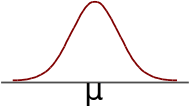
\includegraphics[scale=0.5]{img/introduccion/normal}};
\node at (8,3.6) [fill=color1,single arrow,shape border rotate=270,text=white, minimum width=1.2cm, minimum
height=3cm]{
\rotatebox{90}{Est. Inferencial}\phantom{}};
\pause
\node at (4.5,1) [fill=color1,single arrow,shape border rotate=180,text=white, minimum width=1.2cm, minimum
height=3cm]{ Predicción\phantom{}};
\end{tikzpicture}}
\end{center}
\end{frame}
\note{Para acabar con esta introducción a la Estadística, veremos cuáles son las fases por las que suele pasar cualquier
estudio estadístico, y las partes de la Estadística que se encargan de ello.

\begin{enumerate}
\item En general siempre partiremos de una población en la que queremos estudiar un fenómeno, y se hará un diseño previo del
estudio donde se formulen los objetivos del mismo, qué variables se medirán en los individuos de la población, qué
precisión queremos para nuestras conclusiones y qué tamaño muestral será necesario para ello.
\item A continuación se debe extraer una muestra representativa de la población y de esto esto se
encarga el \textbf{muestreo}.
\item El siguiente paso consiste en estudiar las muestra extraída y presentar de manera ordenada y resumida la
información que esta contiene. De esto se encarga la \textbf{estadística descriptiva}.
\item A continuación, la información obtenida es proyectada sobre un modelo matemático que intenta reflejar el
comportamiento de las variables estudiadas en la población. Tras construir este modelo, se deber realizar un
constraste o una crítica del mismo. Si lo que predice el modelo discrepa con lo observado en la muestra, habrá que
reformular el modelo o construir otro nuevo, mientras que si encaja en lo observado en la muestra, lo daremos por válido
y ello nos permitirá hacer predicciones sobre la población de partida con cierta fibilidad.
\end{enumerate}

En esta primera parte del curso nos centraremos en la Estadística Descriptiva, es decir, la que se encarga de describir
la información contenida en la muestra, pero debemos tener presente que la verdadera potencia de la Estadística está en
completar este ciclo y poder llegar a comprender y controlar el fenómeno que afecta a toda la población.
}

\section{Distribución de frecuencias: Tabulación y gráficos}

\mode<presentation>{
%---------------------------------------------------------------------slide----
\begin{frame}
\frametitle{Distribuciones de frecuencias: Tabulació y gráficos}
\tableofcontents[sectionstyle=show/hide,hideothersubsections]
\end{frame}
}


%---------------------------------------------------------------------slide----
\begin{frame}
\frametitle{Estadística descriptiva}
La estadística descriptiva es la parte de la estadística encargada de representar, analizar y resumir la información contenida en la muestra.

Tras el proceso de muestreo, es la siguiente etapa de todo estudio estadístico y suele consistir en:
\begin{enumerate}
\item Clasificar, agrupar y ordenar los datos de la muestra.
\item Tabular y representar gráficamente los datos de acuerdo a sus frecuencias.
\item Calcular medidas que resuman la información que contiene la muestra (\emph{estadísticos muestrales}).
\end{enumerate} 

No tiene poder inferencial $\Rightarrow$ \alert{\emph{No utilizar para sacar conclusiones sobre la población!}} 
\note{Como se vió en el tema introductorio, la estadística trata de conocer las poblaciones a partir del estudio de
muestras. Una vez obtenida la muestra de la población, el siguiente paso en cualquier estudio estadístico es el
análisis descriptivo de la muestra y este es el objeto la estadística descriptiva, que es la parte de la estadística
encargada de representar, analizar y resumir la información contenida en la muestra. El objetivo es exprimir bien la
muestra para sacarle toda la información posible y sintetizar dicha información para hacerla comprensible.

Las tareas que realiza la estadística descriptiva suelen ser:
\begin{enumerate}
\item Clasificar, agrupar y ordenar los datos de la muestra.
\item Representar dichos datos gráficamente y en forma de tablas.
\item Calcular medidas que resuman la información que contiene la muestra (\emph{estadísticos muestrales}).
\end{enumerate} 

Aunque una buena descripción de la muestra facilita el posterior conocimiento de la población, nunca deben sacarse
conclusiones sobre la población a partir de las medidas resumen que aporta la estadística descriptiva, ya que de esto
se encarga la estadística inferencial que se vera más adelante en este curso.}
\end{frame}


%---------------------------------------------------------------------slide----
\begin{frame}
\frametitle{Clasificación de la muestra}
El estudio de una variable estadística comienza por medir la variable en los individuos de la muestra y clasificar los valores obtenidos.

Existen dos formas de clasificar estos valores:
\begin{description}
\item[Sin agrupar]: Ordenar todos los valores obtenidos en la muestra de menor a mayor (si existe orden). 
Se utiliza con atributos y variables discretas con pocos valores diferentes.
\item[Agrupados]: Agrupar los valores en clases (intervalos) y ordenar dichas clases de menor a mayor. 
Se utiliza con variables continuas y con variables discretas con muchos valores diferentes.
\end{description}
\note{La matriz de datos contiene toda la información de la muestra pero resulta difícil de interpretar, por lo que para
sintetizar y resumir esa información se realizan varias tareas que empiezan por la clasificación de los valores. 

Esta clasificación consiste en ordenar los valores de menor a mayor, cuando existe un orden entre dichos valores, o
simplemente en reunir los valores iguales cuando no hay un orden entre ellos.

En las variables cuantitativas, cuando el número de valores distintos es muy grande, estos suelen agruparse en
intervalos.}
\end{frame}


\subsection{Distribución de frecuencias}

%---------------------------------------------------------------------slide----
\begin{frame}
\frametitle{Clasificación de la muestra}
$X=$Estatura
\begin{center}
\tikzsetnextfilename{descriptiva/clasificacion_muestra}
\scalebox{0.6}{% Autor: Alfredo Sánchez Alberca (email:asalber@ceu.es)
% Charts that shows the purpose of Statistics
\begin{tikzpicture}[every label/.style={text=color1}]
\node (sample) at (0,8) {
\includegraphics[height=4cm]{img/descriptiva/muestra.png}}; 
\pause
\node (ordered-sample) at (0,0) {
\includegraphics[height=4cm]{img/descriptiva/muestra_ordenada.png}};
\node at (0,4) [fill=color1,single arrow,shape border rotate=270,minimum height=3cm,text=white, minimum width=4cm]{\huge
\ Clasificación\ \phantom{}};
\end{tikzpicture} }
\end{center}
\note{En este ejemplo tenemos una muestra de 10 individuos en los que se ha medido su estatura. Como se trata de una
variable cuantitativa, la clasificación consiste, primero en ordenar las estaturas de menor a mayor.}
\end{frame}


%---------------------------------------------------------------------slide----
\begin{frame}
\frametitle{Recuento de frecuencias}
$X=$Estatura
\begin{center}
\tikzsetnextfilename{descriptiva/recuento_frecuencias}
\scalebox{0.6}{% Autor: Alfredo Sánchez Alberca (email:asalber@ceu.es)
% Charts that shows the purpose of Statistics
\begin{tikzpicture}[every label/.style={text=color1}]
\node at (0,8) {
\includegraphics[height=4cm]{img/descriptiva/muestra_ordenada.png}}; 
\pause
\node at (0,0) {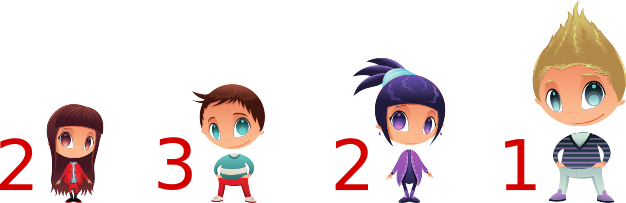
\includegraphics[height=4cm]{img/descriptiva/frecuencias_muestrales.png}};
\node at (0,4) [fill=color1,single arrow,shape border rotate=270,minimum height=3cm,text=white, minimum
width=4cm, align=center]{\huge Recuento\\ \huge frecuencias};
\end{tikzpicture} }
\end{center}
\note{Y a continuación, si hay valores repetidos, contar la frecuencia de repetición de cada estatura o cuántas
estaturas caen en cada uno de los intervalos que hayamos definido en caso de agrupar los datos. Por ejemplo, la primera
estatura se repite dos veces y por tanto tiene frecuencia 2, la segunda estatura se repite tres veces y tiene frecuencia 3 y así sucesivamente. 
}
\end{frame}


%---------------------------------------------------------------------slide----
\begin{frame}
\frametitle{Frecuencias muestrales}
\begin{definicion}[Frecuencias muestrales]
Dada una muestra de tamaño $n$ de una variable $X$, para cada valor $x_i$ de la variable observado en la muestra, se define
\begin{itemize}
\item \highlight{Frecuencia absoluta $n_i$}: Es el número de veces que el valor $x_i$ aparece en la muestra.
\item \highlight{Frecuencia relativa $f_i$}: Es la proporción de veces que el valor $x_i$ aparece en la muestra. 
\[
f_i = \frac{n_i}{n}
\]
\item \highlight{Frecuencia absoluta acumulada $N_i$}: Es el número de valores en la muestra menores o iguales que $x_i$.
\[
N_i = n_1 + \cdots + n_i
\]
\item \highlight{Frecuencia relativa acumulada $F_i$}: Es la proporción de
valores en la muestra menores o iguales que $x_i$.
\[
F_i = \frac{N_i}{n}
\]
\end{itemize}
\end{definicion}
\note{Existen distintos tipos de frecuenicas que pueden calcularse. 
Dada una muestra de tamaño $n$ de una variable $X$, para cada valor de la variable $x_i$ observado en la muestra, se define
\begin{itemize}
\item La frecuencia absoluta, que se representa como $n_i$, es el número de individuos de la
muestra que presentan el valor $x_i$, es decir el número de veces que se repite dicho valor.
\item La frecuencia relativa, que se denota $f_i$, es la proporción de individuos de
la muestra que presentan el valor $x_i$. La frecuencia relativa se calcula dividiendo la frecuencia absoluta entre el
tamaño de la muestra.
\[
f_i = \frac{n_i}{n}
\]
Cuando se multiplica por 100 se convierte en un porcentaje.
\item La frecuencia absoluta acumulada, que se escribe $N_i$, es el número de
individuos de la muestra que presentan un valor menor o igual que $x_i$. Se calcula acumulando las frecuencias
absolutas de los valores menores o iguales a $x_i$ y de ahí su nombre.
\[
N_i = n_1 + \cdots + n_i
\]
\item La frecuencia relativa acumulada, que se escribre $F_i$, es la proporción de
individuos de la muestra que presentan un valor menor o igual que $x_i$. Puede calcularse acumulando las frecuencias
relativas de los valores menores o iguales que $x_i$ o bien dividiendo la frecuencia absoluta cumulada de $x_i$ entre
el tamaño de la muestra.
\[
F_i = \frac{N_i}{n}
\]
Al igual que la frecuencia relativa, si se multiplica por 100 se convierte en el porcentaje acumulado.
\end{itemize}
 }
\end{frame}


%---------------------------------------------------------------------slide----
\begin{frame}
\frametitle{Tabla de frecuencias}
Al conjunto de valores observados en la muestra junto a sus respectivas frecuencias se le denomina \highlight{\textbf{distribución muestral de frecuencias}} y suele representarse mediante una \highlight{\textbf{tabla de frecuencias}}.
\begin{center}
\begin{tabular}{|>{\centering}p{1.8cm}|>{\centering}p{1.8cm}|>{\centering}p{1.8cm}|>{\centering}p{2.2cm}|p{2.2cm}<{\centering}|}
\hline
\highlight{Valores de $X$} & \highlight{Frecuencia Absoluta} & \highlight{Frecuencia Relativa} & \highlight{Frecuencia Absoluta Acumulada} & \highlight{Frecuencia Relativa Acumulada} \\
\hline
$x_1$ & $n_1$ & $f_1$ & $N_1$ & $F_1$\\
$\vdots$ & $\vdots$ & $\vdots$ & $\vdots$ & $\vdots$\\
$x_i$ & $n_i$ & $f_i$ & $N_i$ & $F_i$\\
$\vdots$ & $\vdots$ & $\vdots$ & $\vdots$ & $\vdots$\\
$x_k$ & $n_k$ & $f_k$ & $N_k$ & $F_k$\\
\hline
\end{tabular}
\end{center}
\note{Normalmente las frecuencias muestrales suelen organizarse en forma de tabla en la que cada fila corresponde a un
valor de la variable o un intervalo de valores, que se ordenan, siempre que sea posible, de menor a mayor, y cada
columna corresponde a una frecuencia.

En esta tabla siempre se debe cumplir que la suma de las frecuencias absolutas es igual al tamaño de la muestra, la
suma de las frecuencias relativas vale 1, la última frecuencia absoluta acumulada es el tamaño de la muestra y la
última frecuencia relativa acumulada es 1. De no ser así, habríamos cometido algún error en el cálculo de las
frecuencias.}
\end{frame}


%---------------------------------------------------------------------slide----
\begin{frame}
\frametitle{Tabla de frecuencias}
\framesubtitle{Ejemplo de datos sin agrupar}
El número de hijos en 25 familias es
\begin{center}
1, 2, 4, 2, 2, 2, 3, 2, 1, 1, 0, 2, 2, \\
 0, 2, 2, 1, 2, 2, 3, 1, 2, 2, 1, 2.
\end{center}
La tabla de frecuencias asociada a esta muestra es
\[
\setlength\arraycolsep{3mm}
\setlength\arrayrulewidth{0.5pt}
\begin{array}{rrrrr}
\hline
x_i & n_i & f_i & N_i & F_i\\
\hline
0 & 2 & 0.08 & 2 & 0.08\\
1 & 6 & 0.24 & 8 & 0.32\\
2 & 14 & 0.56 & 22 & 0.88\\
3 & 2  & 0.08 & 24 & 0.96\\
4 & 1 & 0.04 & 25 & 1 \\ 
\hline 
\sum & 25 & 1 \\
\hline
\end{array}
\]
\note{En este ejemplo se han tomado 25 matrimonios en los que se ha medido el número de hijos que tenían. Se trata de
una variable cuantitativa discreta puesto que sólo puede tomar valores enteros positivos y además en la muestra sólo
aparece 5 valores disntintos que son 0, 1, 2, 3 y 4 hijos, por lo que no es necesario agrupar los datos en intervalos.

Para construir la tabla de frecuencias se comienza por el recuento de las frecuencias absolutas. Como puede observarse
en la muestra, hay dos matrimonios que tienen 0 hijos, y por tanto, la frecuencia absoluta del 0 es 2, el 1
aparece 6 veces, el 2, 3 veces, el 3, 2 veces y finalmente el 4 sólo aparece una vez. Observese cómo la suma de las
frecuencias absolutas da 25 que es el tamaño muestral.

A continuación se calculan las frecuencias relativas, simplemente dividiendo cada frecuencia absoluta por el tamaño de
la muestra que es 25. Por ejemplo, la frecuencia relativa del 0 es 2 entre 25 que es 0.08, y es la proporción de
matrimonios en la muestra que tienen 0 hijos.  Si se multiplica por 100 da un 8\%, es decir, el 8\% de los matrimonios
tienen 0 hijos. Obsérvese cómo la suma de las frecuencias relativas vale 1. 

Después se calculan las frecuencias absolutas acumuladas. Así, por ejemplo, la frecuencia absoluta acumulada del 0 es
el número de matrimonios que tienen 0 o menos hijos, y al ser el 0 el menor de los valores de la muestra, coincide con
la su frecuencia absoluta, que vale 2. La frecuencia absoluta acumulada del 1 es el número de matrimonios que tienen 1
o menos hijos, de manera que habría que acumula la frecuencia absoluta del 1 y del 0, es decir, 2 mas 6, que da un
total de 8, y así sucesivamente. En general para calcular cada frecuencia absoluta acumulada se puede tomar la
frecuencia absoluta acumulada anterior y sumarle la frecuencia absoluta del valor. 8+14=22, 22+2=24 y 24+1=25.
Obsérvese cómo la última frecuencia absoluta acumulada vale 25 que es el tamaño de la muestra.

Finalmente, se calculan las frecuencias relativas acumuladas, que pueden calcularse, bien acumulando las frecuencias
relativas del mismo modo que se acumulaban las absolutas, o bien dividiendo las frecuencias absolutas acumuladas por el
tamaño de la muestra. Así, por ejemplo, la frecuencia relativa acumulada del 0 es 2 entre 25, que vale 0.08 y coincide
con su frecuencia relativa. La frecuencia relativa acumulada del 1 es 8 entre 25 que vale 0.32 y es la proporción de
matrimonios en la muestra con 1 o menos hijos. Si se multiplica por 100 tenemos que hay un 32\% de matrimonios con 1 o
menos hijos. Y del mismo modo se calculan el resto de frecuencias relativas acumuladas, hasta llegar a la última que
siempre vale 1.
}
\end{frame}


%---------------------------------------------------------------------slide----
\begin{frame}
\frametitle{Tabla de frecuencias}
\framesubtitle{Ejemplo de datos agrupados}
Las estaturas (en cm) de 30 estudiantes es
\begin{center}
179, 173, 181, 170, 158, 174, 172, 166, 194, 185,\\
162, 187, 198, 177, 178, 165, 154, 188, 166, 171,\\
175, 182, 167, 169, 172, 186, 172, 176, 168, 187.
\end{center}
La tabla de frecuencias asociada a esta muestra es
\[
\setlength\arraycolsep{3mm}
\setlength\arrayrulewidth{0.5pt}
\begin{array}{rrrrr}
\hline
\multicolumn{1}{c}{x_i} & \multicolumn{1}{c}{n_i} & \multicolumn{1}{c}{f_i} & \multicolumn{1}{c}{N_i} & \multicolumn{1}{c}{F_i}\\
\hline
(150,160] & 2 & 0.07 & 2 & 0.07\\
(160,170] & 8 & 0.27 & 10 & 0.34\\
(170,180] & 11 & 0.36 & 21 & 0.70\\
(180,190] & 7  & 0.23 & 28 & 0.93\\
(190,200] & 2 & 0.07 & 30 & 1 \\ 
\hline 
\sum & 30 & 1 \\
\hline
\end{array}
\]
\note{En este otro ejemplo, se han medido las estaturas de 30 universitarios. Ahora se trata de una variable
cuantitativa continua, y como siempre ocurre con este tipo de variables, el número de valores disntintos que aparece en
la muestra suele ser demasiado grande, por lo que se tiene a agruparlos en intervalos.

En este caso se ha optado por construir 5 intervalos de amplitud 10 cm, empezando en 150 cm y terminando en 200 cm. 

El cálculo de frecuencias absolutas es similar al caso anterior, salvo que ahora no se cuenta el número de estaturas
que se repiten, sino el número de estaturas que caen en cada intervalo. Por ejemplo, la frecuencia
absoluta del intervalo $(150,160]$ es 2 ya que en la muestra hay dos personas, una que mide 158 y otra que mide 154, que caerían en este intervalo.
Una vez calculadas las frecuencias abolutas, el cálculo del resto de frecuencias es idéntico al caso de datos no
agrupados.}
\end{frame}


%---------------------------------------------------------------------slide----
\begin{frame}
\frametitle{Construcción de clases}
Cada intervalo de agrupación de datos se denomina \highlight{\textbf{clase}} y el centro del intervalo se llama \highlight{\textbf{marca de clase}}.

A la hora de agrupar los datos en clases hay que tener en cuenta lo siguiente:
\begin{itemize}
\item El número de intervalos no debe ser muy grande ni muy pequeño. 
Una regla orientativa es tomar un número de intervalos próximo $\sqrt{n}$ o $\log_2(n)$. 
\item Los intervalos no deben solaparse y deben cubrir todo el rango de valores.
Es indiferente si se abren por la izquierda y se cierran por la derecha o al revés.
\item El valor más pequeño debe caer dentro del primer intervalo y el más grande dentro del último.
\end{itemize}
\note{Cada intervalo de agrupación de datos se denomina clase y el centro del intervalo se llama
marca de clase. 
Cuando se decide agrupar los datos en clases, hay que tener en cuenta lo siguiente:
\begin{itemize}
\item En primer lugar, el número de intervalos no debe ser muy grande ni muy pequeño. Si hay muchos intervalos, la
tabla será enorme y no sintetizará bien la información de la muestra, mientras que si tomamos muy pocos intervalos, su
amplitud será muy grande y se perderá gran parte de la información que contiene la muestra, ya que cuando un individuo
se cuenta dentro de un intervalo, pierde su valor particular y pasa a ser representado por la marca de clase. Una regla
orientativa es tomar un número de intervalos próximo a la raíz cuadrada del tamaño muestral $\sqrt{n}$.
\item En segundo lugar, los intervalos no deben solaparse, ya que de lo contrario se correría el riesgo de que algún
individuo cayese en dos intervalos distintos, por eso se suelen construir intervalos abiertos por la izquierda y
cerrados por la derecha o al revés, pero siempre siguiendo el mismo criterio. Y también deben cubrir todo el rango de
valores, ya que de lo contrario se correría el riesgo de que algún individuo no caería en ningún intervalo y quedaría
sin contarse.
\item Por último, el valor más pequeño debe caer dentro del primer intervalo y el más grande dentro del último.
\end{itemize}}
\end{frame}


%---------------------------------------------------------------------slide----
\begin{frame}
\frametitle{Tabla de frecuencias}
\framesubtitle{Ejemplo con un atributo}
Los grupos sanguíneos de 30 personas son
\begin{center}
A, B, B, A, AB, 0, 0, A, B, B, A, A, A, A, AB,\\
A, A, A, B, 0, B, B, B, A, A, A, 0, A, AB, 0. 
\end{center}
La tabla de frecuencias asociada a esta muestra es
\[
\setlength\arraycolsep{3mm}
\setlength\arrayrulewidth{0.5pt}
\begin{array}{crr}
\hline
\multicolumn{1}{c}{x_i} & \multicolumn{1}{c}{n_i} & \multicolumn{1}{c}{f_i} \\
\hline
\mbox{0} & 5 & 0.16 \\
\mbox{A} & 14 & 0.47 \\
\mbox{B} & 8 & 0.27 \\
\mbox{AB} & 3 & 0.10 \\
\hline 
\sum & 30 & 1 \\
\hline
\end{array}
\]
\begin{center}
\emph{¿Por qué en este caso no se construyen las columnas de frecuencias acumuladas?}
\end{center}
\note{En este otro ejemplo, se ha medido el grupo sanguíneo de un grupo de 30 personas. Ahora se trata de un atributo
nominal, de manera que como no hay orden entre sus valores, puden ordenarse de cualquier manera en la tabla de
frecuencias, pero el cálculo de frecuencias se realiza como en casos anteriores, con la particularidad de que en este
caso no tiene sentido calcular las frecuencias acumuladas. ¿Te imaginas por qué?}
\end{frame}


\subsection{Representaciones gráficas}

%---------------------------------------------------------------------slide----
\begin{frame}
\frametitle{Representaciones gráficas}
Es habitual representar la distribución muestral de frecuencias de forma gráfica.

Dependiendo del tipo de variable y de si se han agrupado o no los datos, se utilizan distintos tipos de gráficos:
\begin{itemize}
\item Diagrama de barras
\item Histograma
\item Diagrama de líneas
\item Digrama de sectores
\end{itemize}

\note{Habitualmente las frecuencias también suelen representarse de manera gráfica. Dependiendo del tipo de variable y
de si se han agrupado o no los datos, se utilizan distintos tipos de gráficos, entre los que cabe destacar los
diagramas de barras, los histogramas y los diagramas de sectores. Veamos un ejemplo de cada uno de ellos.}
\end{frame}


%---------------------------------------------------------------------slide----
\begin{frame}
\frametitle{Diagrama de barras}
Un \highlight{diagrama de barras} consiste en un conjunto de barras, una para cada valor o categoría de la variabe, dibujadas en unos ejes cartesianos.

Habitualmente os valores o categorías de la variable se representan en el eje $X$, y las frecuencias en el eje $Y$.
Para cada valor o categoría de la variabe se dibuja una barra de altura la correspondiente frecuencia. 
La anchura de la barra es indiferente pero debe haber una separación clara entre las barras.

Dependiendo de la frecuencia representada en el eje $Y$ se tienen distintos tipos de diagramas de barras.

A veces se dibuja un polígono, conocido como \highlight{\textbf{polígono de frecuencias}}, uniendo los puntos más altos de cada barra con segmentos.
\end{frame}


%---------------------------------------------------------------------slide----
\begin{frame}
\frametitle{Diagrama de barras de frecuencias absolutas}
\framesubtitle{Datos sin agrupar}
\begin{center}
\tikzsetnextfilename{descriptiva/diagrama_barras_frecuencia_absoluta}
\scalebox{0.6}{% Created by tikzDevice version 0.8.1 on 2015-11-09 17:42:57
% !TEX encoding = UTF-8 Unicode
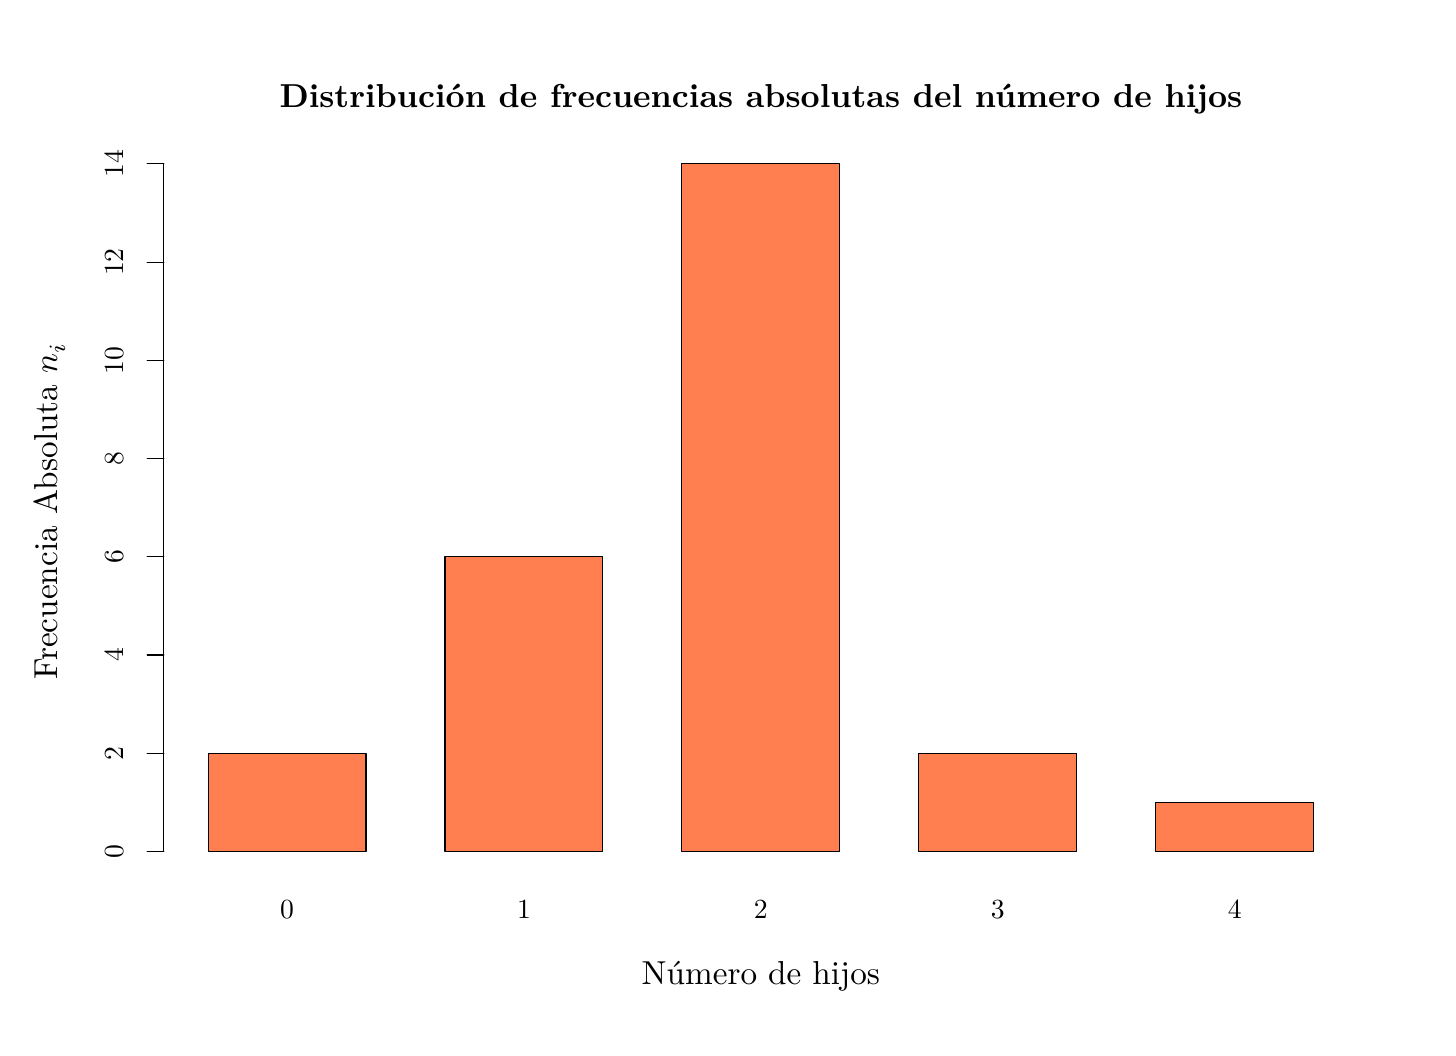
\begin{tikzpicture}[x=1pt,y=1pt]
\definecolor{fillColor}{RGB}{255,255,255}
\path[use as bounding box,fill=fillColor,fill opacity=0.00] (0,0) rectangle (505.89,361.35);
\begin{scope}
\path[clip] (  0.00,  0.00) rectangle (505.89,361.35);
\definecolor{drawColor}{RGB}{0,0,0}
\definecolor{fillColor}{RGB}{255,127,80}

\path[draw=drawColor,line width= 0.4pt,line join=round,line cap=round,fill=fillColor] ( 65.18, 63.68) rectangle (122.26, 99.18);

\path[draw=drawColor,line width= 0.4pt,line join=round,line cap=round,fill=fillColor] (150.79, 63.68) rectangle (207.87,170.17);

\path[draw=drawColor,line width= 0.4pt,line join=round,line cap=round,fill=fillColor] (236.41, 63.68) rectangle (293.48,312.15);

\path[draw=drawColor,line width= 0.4pt,line join=round,line cap=round,fill=fillColor] (322.02, 63.68) rectangle (379.10, 99.18);

\path[draw=drawColor,line width= 0.4pt,line join=round,line cap=round,fill=fillColor] (407.63, 63.68) rectangle (464.71, 81.43);
\end{scope}
\begin{scope}
\path[clip] (  0.00,  0.00) rectangle (505.89,361.35);
\definecolor{drawColor}{RGB}{0,0,0}

\node[text=drawColor,anchor=base,inner sep=0pt, outer sep=0pt, scale=  1.00] at ( 93.72, 39.60) {0};

\node[text=drawColor,anchor=base,inner sep=0pt, outer sep=0pt, scale=  1.00] at (179.33, 39.60) {1};

\node[text=drawColor,anchor=base,inner sep=0pt, outer sep=0pt, scale=  1.00] at (264.94, 39.60) {2};

\node[text=drawColor,anchor=base,inner sep=0pt, outer sep=0pt, scale=  1.00] at (350.56, 39.60) {3};

\node[text=drawColor,anchor=base,inner sep=0pt, outer sep=0pt, scale=  1.00] at (436.17, 39.60) {4};
\end{scope}
\begin{scope}
\path[clip] (  0.00,  0.00) rectangle (505.89,361.35);
\definecolor{drawColor}{RGB}{0,0,0}

\node[text=drawColor,anchor=base,inner sep=0pt, outer sep=0pt, scale=  1.20] at (264.94,332.61) {\bfseries Distribución de frecuencias absolutas del número de hijos};

\node[text=drawColor,anchor=base,inner sep=0pt, outer sep=0pt, scale=  1.20] at (264.94, 15.60) {Número de hijos};

\node[text=drawColor,rotate= 90.00,anchor=base,inner sep=0pt, outer sep=0pt, scale=  1.20] at ( 10.80,186.67) {Frecuencia Absoluta $n_i$};
\end{scope}
\begin{scope}
\path[clip] (  0.00,  0.00) rectangle (505.89,361.35);
\definecolor{drawColor}{RGB}{0,0,0}

\path[draw=drawColor,line width= 0.4pt,line join=round,line cap=round] ( 49.20, 63.68) -- ( 49.20,312.15);

\path[draw=drawColor,line width= 0.4pt,line join=round,line cap=round] ( 49.20, 63.68) -- ( 43.20, 63.68);

\path[draw=drawColor,line width= 0.4pt,line join=round,line cap=round] ( 49.20, 99.18) -- ( 43.20, 99.18);

\path[draw=drawColor,line width= 0.4pt,line join=round,line cap=round] ( 49.20,134.67) -- ( 43.20,134.67);

\path[draw=drawColor,line width= 0.4pt,line join=round,line cap=round] ( 49.20,170.17) -- ( 43.20,170.17);

\path[draw=drawColor,line width= 0.4pt,line join=round,line cap=round] ( 49.20,205.66) -- ( 43.20,205.66);

\path[draw=drawColor,line width= 0.4pt,line join=round,line cap=round] ( 49.20,241.16) -- ( 43.20,241.16);

\path[draw=drawColor,line width= 0.4pt,line join=round,line cap=round] ( 49.20,276.65) -- ( 43.20,276.65);

\path[draw=drawColor,line width= 0.4pt,line join=round,line cap=round] ( 49.20,312.15) -- ( 43.20,312.15);

\node[text=drawColor,rotate= 90.00,anchor=base,inner sep=0pt, outer sep=0pt, scale=  1.00] at ( 34.80, 63.68) {0};

\node[text=drawColor,rotate= 90.00,anchor=base,inner sep=0pt, outer sep=0pt, scale=  1.00] at ( 34.80, 99.18) {2};

\node[text=drawColor,rotate= 90.00,anchor=base,inner sep=0pt, outer sep=0pt, scale=  1.00] at ( 34.80,134.67) {4};

\node[text=drawColor,rotate= 90.00,anchor=base,inner sep=0pt, outer sep=0pt, scale=  1.00] at ( 34.80,170.17) {6};

\node[text=drawColor,rotate= 90.00,anchor=base,inner sep=0pt, outer sep=0pt, scale=  1.00] at ( 34.80,205.66) {8};

\node[text=drawColor,rotate= 90.00,anchor=base,inner sep=0pt, outer sep=0pt, scale=  1.00] at ( 34.80,241.16) {10};

\node[text=drawColor,rotate= 90.00,anchor=base,inner sep=0pt, outer sep=0pt, scale=  1.00] at ( 34.80,276.65) {12};

\node[text=drawColor,rotate= 90.00,anchor=base,inner sep=0pt, outer sep=0pt, scale=  1.00] at ( 34.80,312.15) {14};
\end{scope}

\end{tikzpicture}
}
\end{center}
\note{El diagrama de barras se utiliza con variables cuantitativas y datos sin agrupar y consiste en un sistema de ejes
cartesianos en el que se representan los valores de la variable en el eje de abscisas y las frecuencias
correspondientes en el eje de ordenadas, de manera que sobre cada valor se levanta una barra de altura la
correspondiente frecuencia. La frecuencia representada puede ser cualquiera de las cuatro vistas por lo que hay cuatro
tipos de diagramas de barras. 

En este ejemplo tenemos el diagrama de barras de frecuencias absolutas correspondiente a la muestra de 25 matrimonios
en los que se midió el número de hijos. Como puede observarse la barra que hay sobre el 0 tiene altura 2 por que la
frecuencia absoluta del 0 es 2, la barra que hay sobre el 1 tiene altura 6 porque el 1 tiene frecuencia 6, etc.}
\end{frame}


%---------------------------------------------------------------------slide----
\begin{frame}
\frametitle{Diagrama de líneas o Polígono de frecuencias absolutas}
\framesubtitle{Datos sin agrupar}
\begin{center}
\tikzsetnextfilename{descriptiva/poligono_frecuencia_absoluta}
\scalebox{0.6}{% Created by tikzDevice version 0.8.1 on 2016-01-24 02:13:24
% !TEX encoding = UTF-8 Unicode
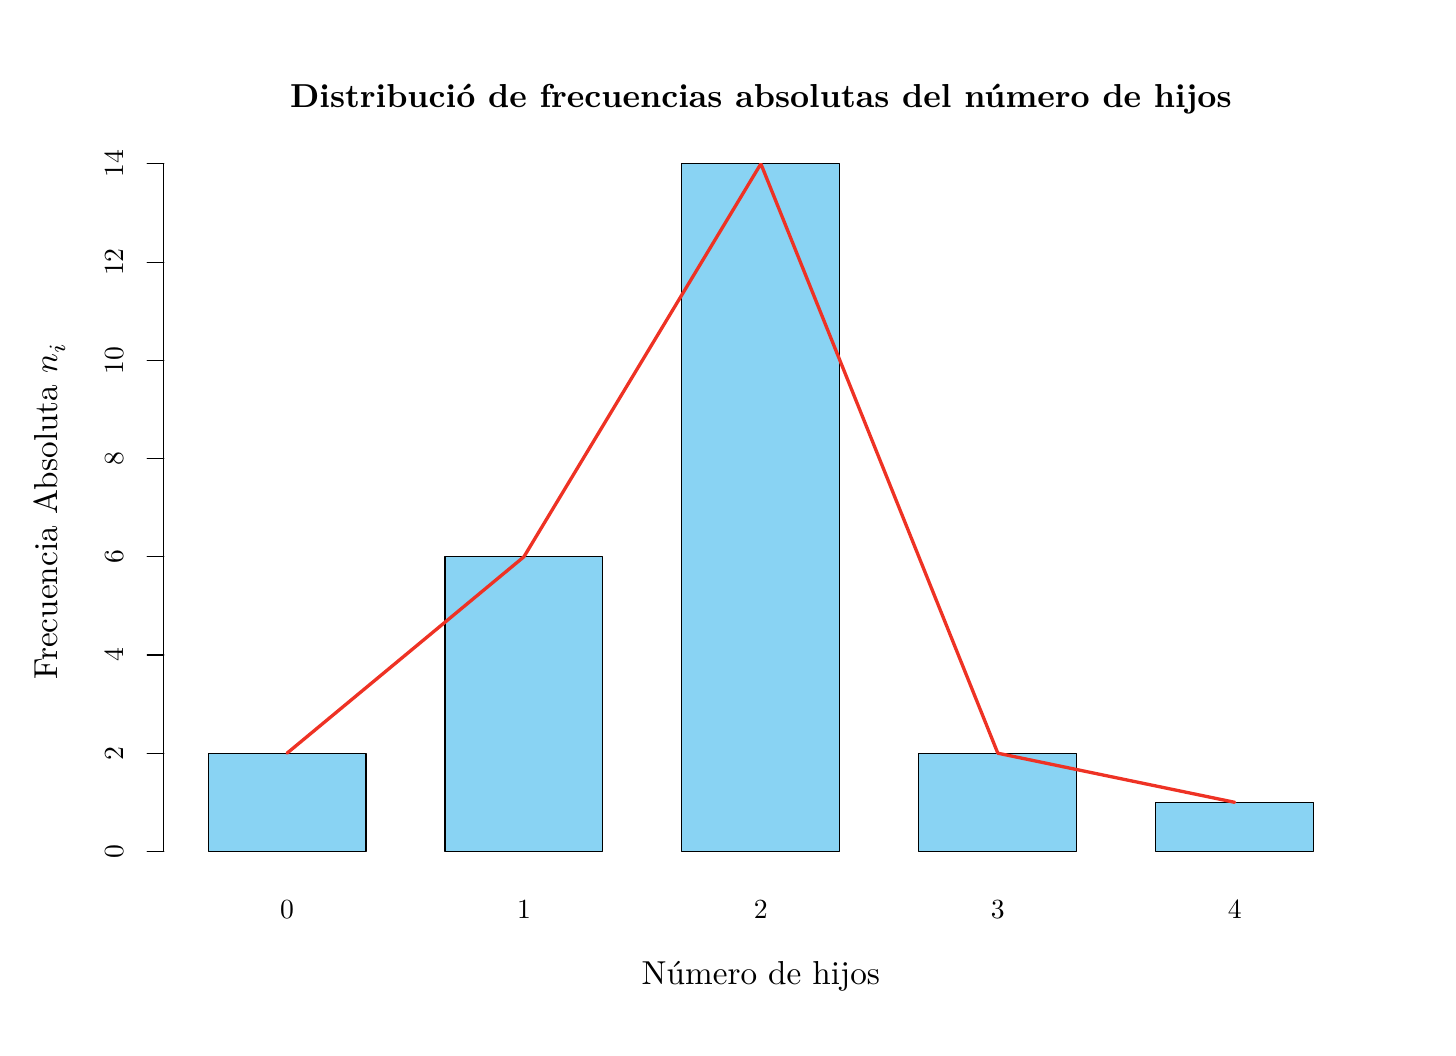
\begin{tikzpicture}[x=1pt,y=1pt]
\definecolor{fillColor}{RGB}{255,255,255}
\path[use as bounding box,fill=fillColor,fill opacity=0.00] (0,0) rectangle (505.89,361.35);
\begin{scope}
\path[clip] (  0.00,  0.00) rectangle (505.89,361.35);
\definecolor{drawColor}{RGB}{0,0,0}
\definecolor{fillColor}{RGB}{137,211,243}

\path[draw=drawColor,line width= 0.4pt,line join=round,line cap=round,fill=fillColor] ( 65.18, 63.68) rectangle (122.26, 99.18);

\path[draw=drawColor,line width= 0.4pt,line join=round,line cap=round,fill=fillColor] (150.79, 63.68) rectangle (207.87,170.17);

\path[draw=drawColor,line width= 0.4pt,line join=round,line cap=round,fill=fillColor] (236.41, 63.68) rectangle (293.48,312.15);

\path[draw=drawColor,line width= 0.4pt,line join=round,line cap=round,fill=fillColor] (322.02, 63.68) rectangle (379.10, 99.18);

\path[draw=drawColor,line width= 0.4pt,line join=round,line cap=round,fill=fillColor] (407.63, 63.68) rectangle (464.71, 81.43);
\end{scope}
\begin{scope}
\path[clip] (  0.00,  0.00) rectangle (505.89,361.35);
\definecolor{drawColor}{RGB}{0,0,0}

\node[text=drawColor,anchor=base,inner sep=0pt, outer sep=0pt, scale=  1.00] at ( 93.72, 39.60) {0};

\node[text=drawColor,anchor=base,inner sep=0pt, outer sep=0pt, scale=  1.00] at (179.33, 39.60) {1};

\node[text=drawColor,anchor=base,inner sep=0pt, outer sep=0pt, scale=  1.00] at (264.94, 39.60) {2};

\node[text=drawColor,anchor=base,inner sep=0pt, outer sep=0pt, scale=  1.00] at (350.56, 39.60) {3};

\node[text=drawColor,anchor=base,inner sep=0pt, outer sep=0pt, scale=  1.00] at (436.17, 39.60) {4};
\end{scope}
\begin{scope}
\path[clip] (  0.00,  0.00) rectangle (505.89,361.35);
\definecolor{drawColor}{RGB}{0,0,0}

\node[text=drawColor,anchor=base,inner sep=0pt, outer sep=0pt, scale=  1.20] at (264.94,332.61) {\bfseries Distribució de frecuencias absolutas del número de hijos};

\node[text=drawColor,anchor=base,inner sep=0pt, outer sep=0pt, scale=  1.20] at (264.94, 15.60) {Número de hijos};

\node[text=drawColor,rotate= 90.00,anchor=base,inner sep=0pt, outer sep=0pt, scale=  1.20] at ( 10.80,186.67) {Frecuencia Absoluta $n_i$};
\end{scope}
\begin{scope}
\path[clip] (  0.00,  0.00) rectangle (505.89,361.35);
\definecolor{drawColor}{RGB}{0,0,0}

\path[draw=drawColor,line width= 0.4pt,line join=round,line cap=round] ( 49.20, 63.68) -- ( 49.20,312.15);

\path[draw=drawColor,line width= 0.4pt,line join=round,line cap=round] ( 49.20, 63.68) -- ( 43.20, 63.68);

\path[draw=drawColor,line width= 0.4pt,line join=round,line cap=round] ( 49.20, 99.18) -- ( 43.20, 99.18);

\path[draw=drawColor,line width= 0.4pt,line join=round,line cap=round] ( 49.20,134.67) -- ( 43.20,134.67);

\path[draw=drawColor,line width= 0.4pt,line join=round,line cap=round] ( 49.20,170.17) -- ( 43.20,170.17);

\path[draw=drawColor,line width= 0.4pt,line join=round,line cap=round] ( 49.20,205.66) -- ( 43.20,205.66);

\path[draw=drawColor,line width= 0.4pt,line join=round,line cap=round] ( 49.20,241.16) -- ( 43.20,241.16);

\path[draw=drawColor,line width= 0.4pt,line join=round,line cap=round] ( 49.20,276.65) -- ( 43.20,276.65);

\path[draw=drawColor,line width= 0.4pt,line join=round,line cap=round] ( 49.20,312.15) -- ( 43.20,312.15);

\node[text=drawColor,rotate= 90.00,anchor=base,inner sep=0pt, outer sep=0pt, scale=  1.00] at ( 34.80, 63.68) {0};

\node[text=drawColor,rotate= 90.00,anchor=base,inner sep=0pt, outer sep=0pt, scale=  1.00] at ( 34.80, 99.18) {2};

\node[text=drawColor,rotate= 90.00,anchor=base,inner sep=0pt, outer sep=0pt, scale=  1.00] at ( 34.80,134.67) {4};

\node[text=drawColor,rotate= 90.00,anchor=base,inner sep=0pt, outer sep=0pt, scale=  1.00] at ( 34.80,170.17) {6};

\node[text=drawColor,rotate= 90.00,anchor=base,inner sep=0pt, outer sep=0pt, scale=  1.00] at ( 34.80,205.66) {8};

\node[text=drawColor,rotate= 90.00,anchor=base,inner sep=0pt, outer sep=0pt, scale=  1.00] at ( 34.80,241.16) {10};

\node[text=drawColor,rotate= 90.00,anchor=base,inner sep=0pt, outer sep=0pt, scale=  1.00] at ( 34.80,276.65) {12};

\node[text=drawColor,rotate= 90.00,anchor=base,inner sep=0pt, outer sep=0pt, scale=  1.00] at ( 34.80,312.15) {14};
\end{scope}
\begin{scope}
\path[clip] ( 49.20, 61.20) rectangle (480.69,312.15);
\definecolor{drawColor}{RGB}{238,50,36}

\path[draw=drawColor,line width= 1.2pt,line join=round,line cap=round] ( 93.72, 99.18) --
	(179.33,170.17) --
	(264.94,312.15) --
	(350.56, 99.18) --
	(436.17, 81.43);
\end{scope}
\end{tikzpicture}
}
\end{center}
\note{A veces, sobre el diagrama de barras se suele representar un polígono conocido como polígono de frecuencias, y
que en el caso de las frecuencias absolutas se construye uniendo los puntos más altos de las barras mediante segmento.
}
\end{frame}


%---------------------------------------------------------------------slide----
\begin{frame}
\frametitle{Diagrama de barras de frecuencias acumuladas}
\framesubtitle{Datos sin agrupar}
\begin{center}
\tikzsetnextfilename{descriptiva/diagrama_barras_frecuencia_acumulada}
\scalebox{0.6}{% Created by tikzDevice version 0.8.1 on 2015-11-09 17:42:58
% !TEX encoding = UTF-8 Unicode
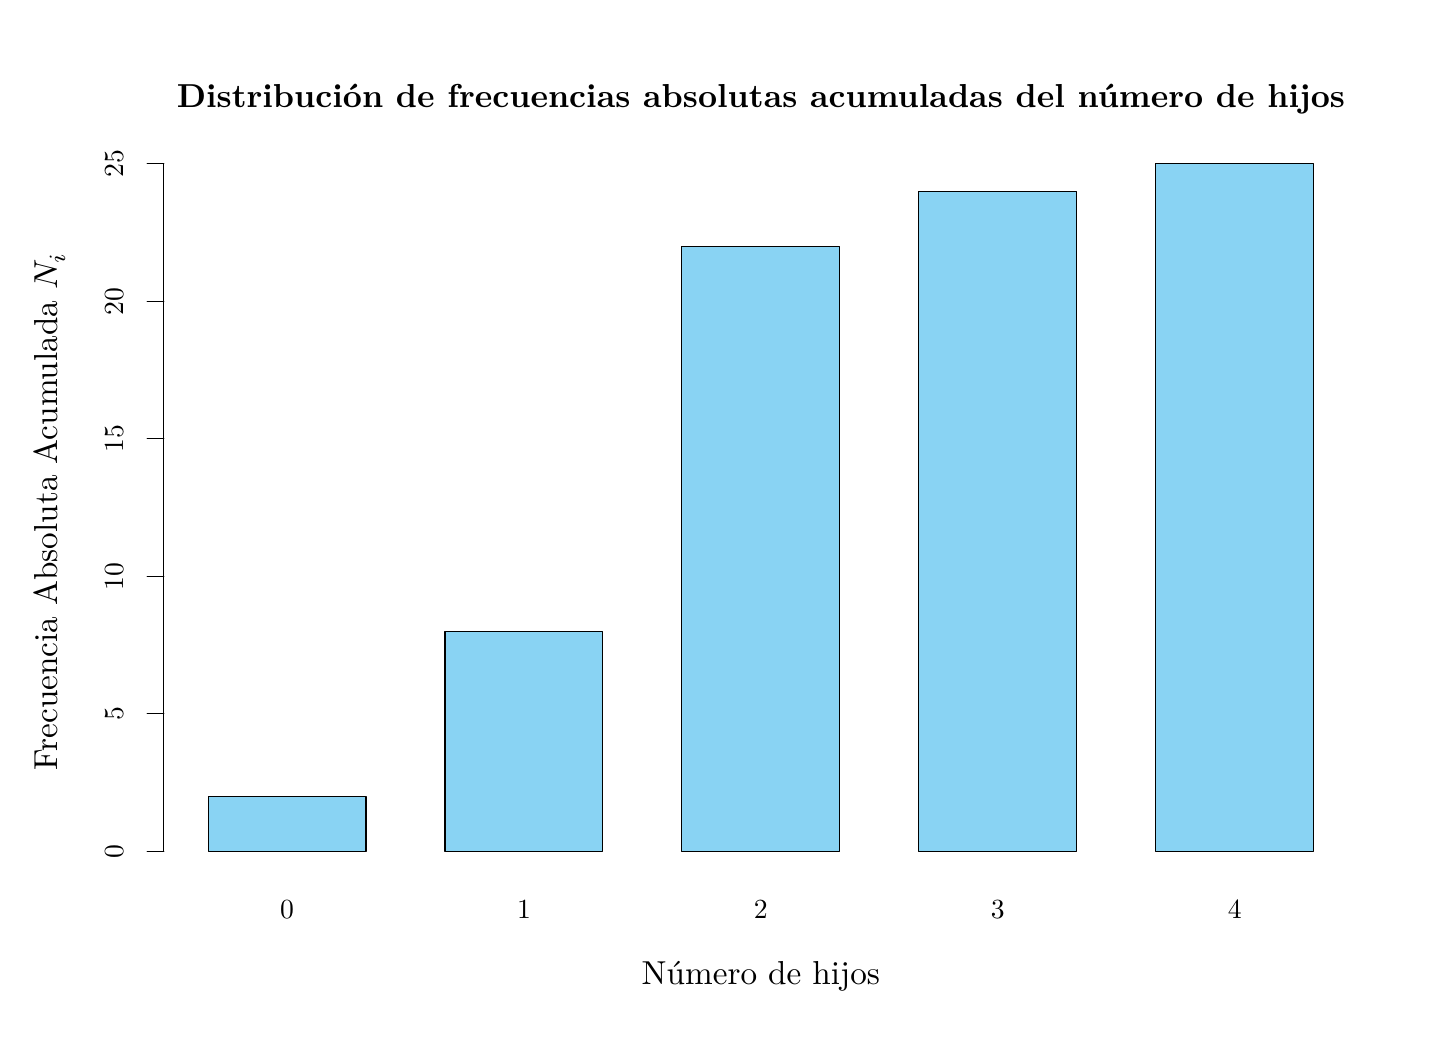
\begin{tikzpicture}[x=1pt,y=1pt]
\definecolor{fillColor}{RGB}{255,255,255}
\path[use as bounding box,fill=fillColor,fill opacity=0.00] (0,0) rectangle (505.89,361.35);
\begin{scope}
\path[clip] (  0.00,  0.00) rectangle (505.89,361.35);
\definecolor{drawColor}{RGB}{0,0,0}
\definecolor{fillColor}{RGB}{137,211,243}

\path[draw=drawColor,line width= 0.4pt,line join=round,line cap=round,fill=fillColor] ( 65.18, 63.68) rectangle (122.26, 83.56);

\path[draw=drawColor,line width= 0.4pt,line join=round,line cap=round,fill=fillColor] (150.79, 63.68) rectangle (207.87,143.19);

\path[draw=drawColor,line width= 0.4pt,line join=round,line cap=round,fill=fillColor] (236.41, 63.68) rectangle (293.48,282.33);

\path[draw=drawColor,line width= 0.4pt,line join=round,line cap=round,fill=fillColor] (322.02, 63.68) rectangle (379.10,302.21);

\path[draw=drawColor,line width= 0.4pt,line join=round,line cap=round,fill=fillColor] (407.63, 63.68) rectangle (464.71,312.15);
\end{scope}
\begin{scope}
\path[clip] (  0.00,  0.00) rectangle (505.89,361.35);
\definecolor{drawColor}{RGB}{0,0,0}

\node[text=drawColor,anchor=base,inner sep=0pt, outer sep=0pt, scale=  1.00] at ( 93.72, 39.60) {0};

\node[text=drawColor,anchor=base,inner sep=0pt, outer sep=0pt, scale=  1.00] at (179.33, 39.60) {1};

\node[text=drawColor,anchor=base,inner sep=0pt, outer sep=0pt, scale=  1.00] at (264.94, 39.60) {2};

\node[text=drawColor,anchor=base,inner sep=0pt, outer sep=0pt, scale=  1.00] at (350.56, 39.60) {3};

\node[text=drawColor,anchor=base,inner sep=0pt, outer sep=0pt, scale=  1.00] at (436.17, 39.60) {4};
\end{scope}
\begin{scope}
\path[clip] (  0.00,  0.00) rectangle (505.89,361.35);
\definecolor{drawColor}{RGB}{0,0,0}

\node[text=drawColor,anchor=base,inner sep=0pt, outer sep=0pt, scale=  1.20] at (264.94,332.61) {\bfseries Distribución de frecuencias absolutas acumuladas del número de hijos};

\node[text=drawColor,anchor=base,inner sep=0pt, outer sep=0pt, scale=  1.20] at (264.94, 15.60) {Número de hijos};

\node[text=drawColor,rotate= 90.00,anchor=base,inner sep=0pt, outer sep=0pt, scale=  1.20] at ( 10.80,186.67) {Frecuencia Absoluta Acumulada $N_i$};
\end{scope}
\begin{scope}
\path[clip] (  0.00,  0.00) rectangle (505.89,361.35);
\definecolor{drawColor}{RGB}{0,0,0}

\path[draw=drawColor,line width= 0.4pt,line join=round,line cap=round] ( 49.20, 63.68) -- ( 49.20,312.15);

\path[draw=drawColor,line width= 0.4pt,line join=round,line cap=round] ( 49.20, 63.68) -- ( 43.20, 63.68);

\path[draw=drawColor,line width= 0.4pt,line join=round,line cap=round] ( 49.20,113.38) -- ( 43.20,113.38);

\path[draw=drawColor,line width= 0.4pt,line join=round,line cap=round] ( 49.20,163.07) -- ( 43.20,163.07);

\path[draw=drawColor,line width= 0.4pt,line join=round,line cap=round] ( 49.20,212.76) -- ( 43.20,212.76);

\path[draw=drawColor,line width= 0.4pt,line join=round,line cap=round] ( 49.20,262.46) -- ( 43.20,262.46);

\path[draw=drawColor,line width= 0.4pt,line join=round,line cap=round] ( 49.20,312.15) -- ( 43.20,312.15);

\node[text=drawColor,rotate= 90.00,anchor=base,inner sep=0pt, outer sep=0pt, scale=  1.00] at ( 34.80, 63.68) {0};

\node[text=drawColor,rotate= 90.00,anchor=base,inner sep=0pt, outer sep=0pt, scale=  1.00] at ( 34.80,113.38) {5};

\node[text=drawColor,rotate= 90.00,anchor=base,inner sep=0pt, outer sep=0pt, scale=  1.00] at ( 34.80,163.07) {10};

\node[text=drawColor,rotate= 90.00,anchor=base,inner sep=0pt, outer sep=0pt, scale=  1.00] at ( 34.80,212.76) {15};

\node[text=drawColor,rotate= 90.00,anchor=base,inner sep=0pt, outer sep=0pt, scale=  1.00] at ( 34.80,262.46) {20};

\node[text=drawColor,rotate= 90.00,anchor=base,inner sep=0pt, outer sep=0pt, scale=  1.00] at ( 34.80,312.15) {25};
\end{scope}

\end{tikzpicture}
}
\end{center}
\note{En este gráfico aparece el diagrama de barras de frecuencias absolutas acumuladas, y como puede apreciarse, al
tratarse de frecuencias acumuladas, las barras van creciendo progresivamente hasta que la última barra tiene la altura
del tamaño muestral.}
\end{frame}


%---------------------------------------------------------------------slide----
\begin{frame}
\frametitle{Diagrama de línea o polígono de frecuencias absolutas acumuladas}
\framesubtitle{Datos sin agrupar}
\begin{center}
\tikzsetnextfilename{descriptiva/poligono_frecuencia_acumulada}
\scalebox{0.6}{% Created by tikzDevice version 0.8.1 on 2015-11-09 17:45:22
% !TEX encoding = UTF-8 Unicode
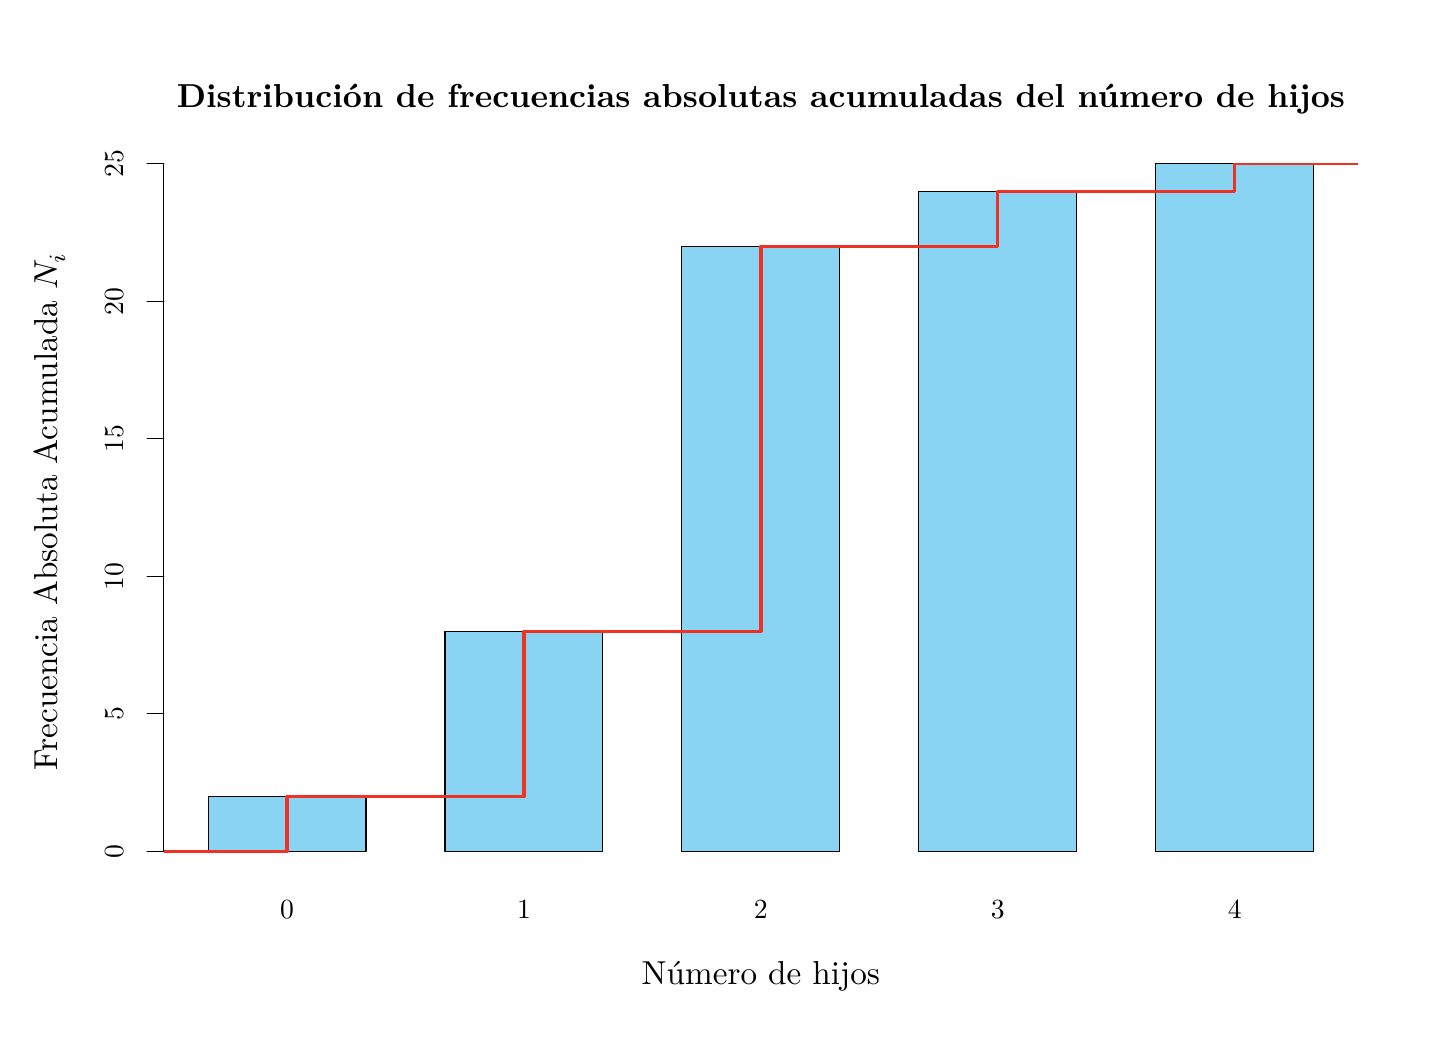
\begin{tikzpicture}[x=1pt,y=1pt]
\definecolor{fillColor}{RGB}{255,255,255}
\path[use as bounding box,fill=fillColor,fill opacity=0.00] (0,0) rectangle (505.89,361.35);
\begin{scope}
\path[clip] (  0.00,  0.00) rectangle (505.89,361.35);
\definecolor{drawColor}{RGB}{0,0,0}
\definecolor{fillColor}{RGB}{137,211,243}

\path[draw=drawColor,line width= 0.4pt,line join=round,line cap=round,fill=fillColor] ( 65.18, 63.68) rectangle (122.26, 83.56);

\path[draw=drawColor,line width= 0.4pt,line join=round,line cap=round,fill=fillColor] (150.79, 63.68) rectangle (207.87,143.19);

\path[draw=drawColor,line width= 0.4pt,line join=round,line cap=round,fill=fillColor] (236.41, 63.68) rectangle (293.48,282.33);

\path[draw=drawColor,line width= 0.4pt,line join=round,line cap=round,fill=fillColor] (322.02, 63.68) rectangle (379.10,302.21);

\path[draw=drawColor,line width= 0.4pt,line join=round,line cap=round,fill=fillColor] (407.63, 63.68) rectangle (464.71,312.15);
\end{scope}
\begin{scope}
\path[clip] (  0.00,  0.00) rectangle (505.89,361.35);
\definecolor{drawColor}{RGB}{0,0,0}

\node[text=drawColor,anchor=base,inner sep=0pt, outer sep=0pt, scale=  1.00] at ( 93.72, 39.60) {0};

\node[text=drawColor,anchor=base,inner sep=0pt, outer sep=0pt, scale=  1.00] at (179.33, 39.60) {1};

\node[text=drawColor,anchor=base,inner sep=0pt, outer sep=0pt, scale=  1.00] at (264.94, 39.60) {2};

\node[text=drawColor,anchor=base,inner sep=0pt, outer sep=0pt, scale=  1.00] at (350.56, 39.60) {3};

\node[text=drawColor,anchor=base,inner sep=0pt, outer sep=0pt, scale=  1.00] at (436.17, 39.60) {4};
\end{scope}
\begin{scope}
\path[clip] (  0.00,  0.00) rectangle (505.89,361.35);
\definecolor{drawColor}{RGB}{0,0,0}

\node[text=drawColor,anchor=base,inner sep=0pt, outer sep=0pt, scale=  1.20] at (264.94,332.61) {\bfseries Distribución de frecuencias absolutas acumuladas del número de hijos};

\node[text=drawColor,anchor=base,inner sep=0pt, outer sep=0pt, scale=  1.20] at (264.94, 15.60) {Número de hijos};

\node[text=drawColor,rotate= 90.00,anchor=base,inner sep=0pt, outer sep=0pt, scale=  1.20] at ( 10.80,186.67) {Frecuencia Absoluta Acumulada $N_i$};
\end{scope}
\begin{scope}
\path[clip] (  0.00,  0.00) rectangle (505.89,361.35);
\definecolor{drawColor}{RGB}{0,0,0}

\path[draw=drawColor,line width= 0.4pt,line join=round,line cap=round] ( 49.20, 63.68) -- ( 49.20,312.15);

\path[draw=drawColor,line width= 0.4pt,line join=round,line cap=round] ( 49.20, 63.68) -- ( 43.20, 63.68);

\path[draw=drawColor,line width= 0.4pt,line join=round,line cap=round] ( 49.20,113.38) -- ( 43.20,113.38);

\path[draw=drawColor,line width= 0.4pt,line join=round,line cap=round] ( 49.20,163.07) -- ( 43.20,163.07);

\path[draw=drawColor,line width= 0.4pt,line join=round,line cap=round] ( 49.20,212.76) -- ( 43.20,212.76);

\path[draw=drawColor,line width= 0.4pt,line join=round,line cap=round] ( 49.20,262.46) -- ( 43.20,262.46);

\path[draw=drawColor,line width= 0.4pt,line join=round,line cap=round] ( 49.20,312.15) -- ( 43.20,312.15);

\node[text=drawColor,rotate= 90.00,anchor=base,inner sep=0pt, outer sep=0pt, scale=  1.00] at ( 34.80, 63.68) {0};

\node[text=drawColor,rotate= 90.00,anchor=base,inner sep=0pt, outer sep=0pt, scale=  1.00] at ( 34.80,113.38) {5};

\node[text=drawColor,rotate= 90.00,anchor=base,inner sep=0pt, outer sep=0pt, scale=  1.00] at ( 34.80,163.07) {10};

\node[text=drawColor,rotate= 90.00,anchor=base,inner sep=0pt, outer sep=0pt, scale=  1.00] at ( 34.80,212.76) {15};

\node[text=drawColor,rotate= 90.00,anchor=base,inner sep=0pt, outer sep=0pt, scale=  1.00] at ( 34.80,262.46) {20};

\node[text=drawColor,rotate= 90.00,anchor=base,inner sep=0pt, outer sep=0pt, scale=  1.00] at ( 34.80,312.15) {25};
\end{scope}
\begin{scope}
\path[clip] ( 49.20, 61.20) rectangle (480.69,312.15);
\definecolor{drawColor}{RGB}{238,50,36}

\path[draw=drawColor,line width= 1.2pt,line join=round,line cap=round] ( 36.64, 63.68) --
	( 93.72, 63.68) --
	( 93.72, 83.56) --
	(179.33, 83.56) --
	(179.33,143.19) --
	(264.94,143.19) --
	(264.94,282.33) --
	(350.56,282.33) --
	(350.56,302.21) --
	(436.17,302.21) --
	(436.17,312.15) --
	(505.89,312.15);
\end{scope}
\end{tikzpicture}
}
\end{center}
\note{El polígono de frecuencias absolutas acumuladas, a diferencia del de absolutas, tiene forma de escalera,
reflejando que la acumulación de individuos se produce a saltos, y no de manera progresiva como podrían entenderse si
simplemente se uniesen los puntos más altos de cada barra. 

Este polígono refleja que la frecuencia absoluta acumulada de cualquier valor anterior al 0 es 0 ya que no hay
matrimonios con menos de 0 hijos. Al llegar al 0 nos encontramos con dos matrimonios que no tienen hijos, y de pronto
la frecuencia absoluta acumulada pasa a valer 2. Del 0 al 1, no nos encontramos nigún valor en la muestra, ya que no
hay matrimonios que tengan entre 0 y 1 hijos, por lo que el polígono continúa con un segmento horizontal sobre el dos,
reflejando que al frecuencia absoluta acumulada se mantiene en 2. Cuando se llega al 1, volvemos a encontrarnos 6
matrimonios con 1 hijo, y el polígon da un salto hasta el 8. Del 1 al dos se mantiene constante en el 8, hasta llegar
al 2 donde vuelve a dar un salto hasta el 22 y así sucesivamente hasta que al final se alcanza el nivel del tamaño
muestral.}
\end{frame}


%---------------------------------------------------------------------slide----
\begin{frame}
\frametitle{Histograma}
Un \highlight{histograma} es similar a un diagrama de barras pero para datos agrupados.

Habitualmente las clases o intervalos de agrupación se representan en el eje $X$, y las frecuencias en el eje $Y$.

Para cada clase se dibuja una barra de altura la correspondiente frecuencia.
A diferencia del diagrama de barras, la anchura del la barra coincide con la anchura de las clases y no hay separación entre dos barras consecutivas.

Dependiendo del tipo de frecuencia representada en el eje $Y$ existen distintos tipos de histogramas.
 
A veces se dibuja un polígono, conocido como \highlight{\textbf{polígono de frecuencias}}, uniendo los puntos más altos de cada barra con segmentos.
\end{frame}


%---------------------------------------------------------------------slide----
\begin{frame}
\frametitle{Histograma de frecuencias absolutas}
\framesubtitle{Datos agrupados}
\begin{center}
\tikzsetnextfilename{descriptiva/histograma_frecuencia_absoluta}
\scalebox{0.6}{% Created by tikzDevice version 0.8.1 on 2015-11-09 19:19:11
% !TEX encoding = UTF-8 Unicode
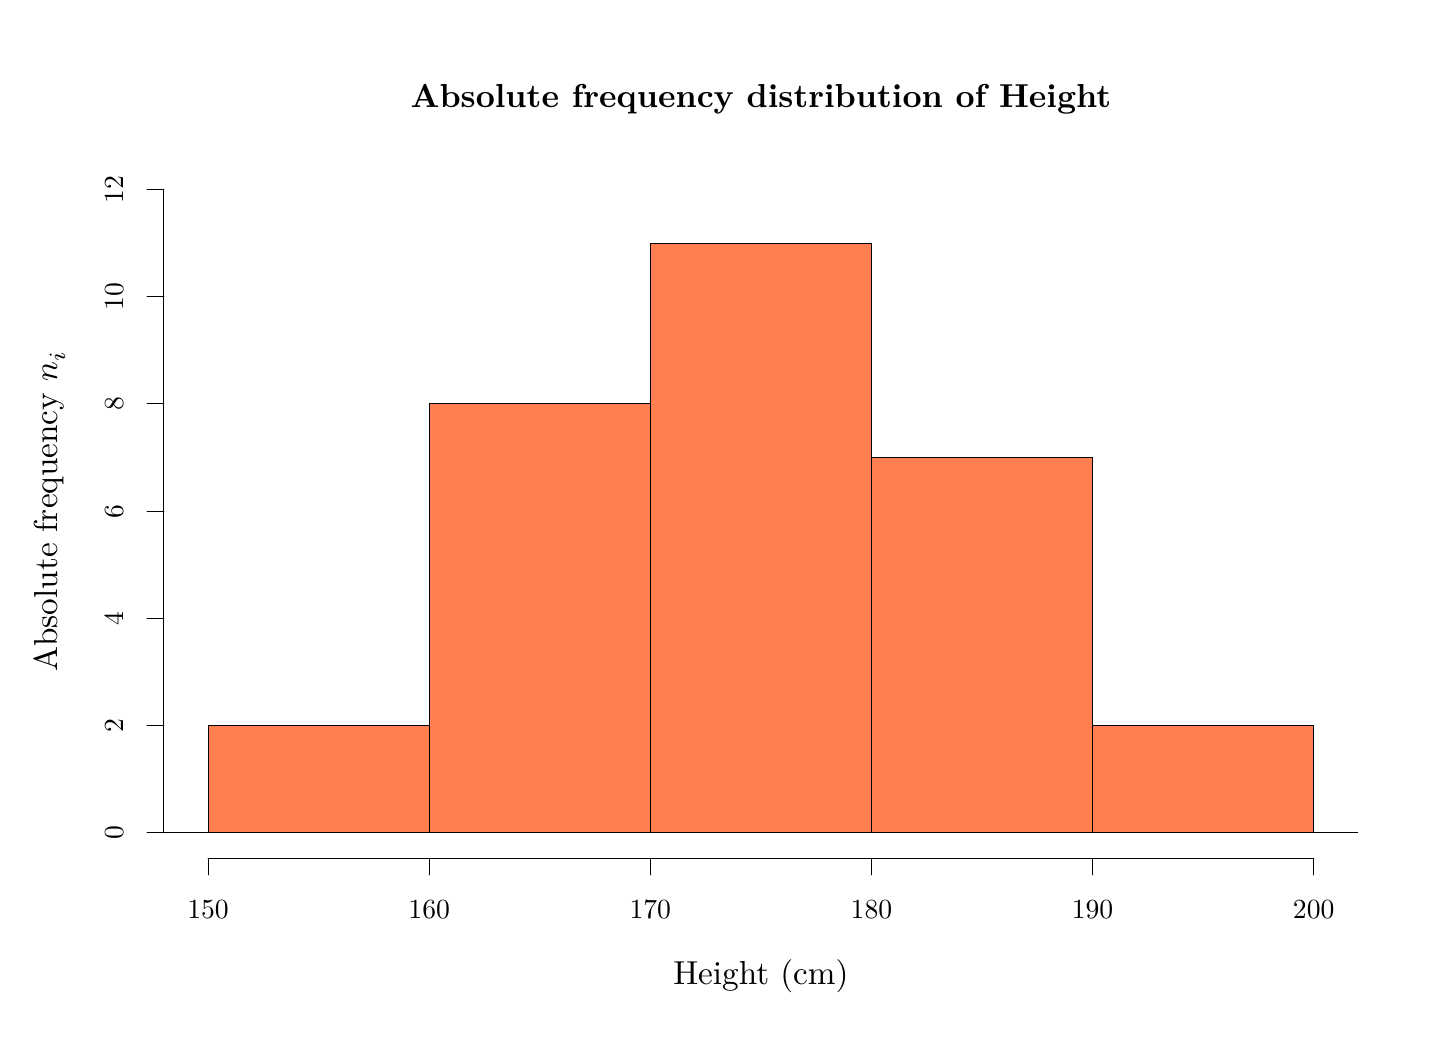
\begin{tikzpicture}[x=1pt,y=1pt]
\definecolor{fillColor}{RGB}{255,255,255}
\path[use as bounding box,fill=fillColor,fill opacity=0.00] (0,0) rectangle (505.89,361.35);
\begin{scope}
\path[clip] (  0.00,  0.00) rectangle (505.89,361.35);
\definecolor{drawColor}{RGB}{0,0,0}

\node[text=drawColor,anchor=base,inner sep=0pt, outer sep=0pt, scale=  1.20] at (264.95,332.61) {\bfseries Absolute frequency distribution of Height};

\node[text=drawColor,anchor=base,inner sep=0pt, outer sep=0pt, scale=  1.20] at (264.95, 15.60) {Height (cm)};

\node[text=drawColor,rotate= 90.00,anchor=base,inner sep=0pt, outer sep=0pt, scale=  1.20] at ( 10.80,186.67) {Absolute frequency $n_i$};
\end{scope}
\begin{scope}
\path[clip] (  0.00,  0.00) rectangle (505.89,361.35);
\definecolor{drawColor}{RGB}{0,0,0}

\path[draw=drawColor,line width= 0.4pt,line join=round,line cap=round] ( 65.18, 61.20) -- (464.71, 61.20);

\path[draw=drawColor,line width= 0.4pt,line join=round,line cap=round] ( 65.18, 61.20) -- ( 65.18, 55.20);

\path[draw=drawColor,line width= 0.4pt,line join=round,line cap=round] (145.09, 61.20) -- (145.09, 55.20);

\path[draw=drawColor,line width= 0.4pt,line join=round,line cap=round] (224.99, 61.20) -- (224.99, 55.20);

\path[draw=drawColor,line width= 0.4pt,line join=round,line cap=round] (304.90, 61.20) -- (304.90, 55.20);

\path[draw=drawColor,line width= 0.4pt,line join=round,line cap=round] (384.80, 61.20) -- (384.80, 55.20);

\path[draw=drawColor,line width= 0.4pt,line join=round,line cap=round] (464.71, 61.20) -- (464.71, 55.20);

\node[text=drawColor,anchor=base,inner sep=0pt, outer sep=0pt, scale=  1.00] at ( 65.18, 39.60) {150};

\node[text=drawColor,anchor=base,inner sep=0pt, outer sep=0pt, scale=  1.00] at (145.09, 39.60) {160};

\node[text=drawColor,anchor=base,inner sep=0pt, outer sep=0pt, scale=  1.00] at (224.99, 39.60) {170};

\node[text=drawColor,anchor=base,inner sep=0pt, outer sep=0pt, scale=  1.00] at (304.90, 39.60) {180};

\node[text=drawColor,anchor=base,inner sep=0pt, outer sep=0pt, scale=  1.00] at (384.80, 39.60) {190};

\node[text=drawColor,anchor=base,inner sep=0pt, outer sep=0pt, scale=  1.00] at (464.71, 39.60) {200};

\path[draw=drawColor,line width= 0.4pt,line join=round,line cap=round] ( 49.20, 70.49) -- ( 49.20,302.86);

\path[draw=drawColor,line width= 0.4pt,line join=round,line cap=round] ( 49.20, 70.49) -- ( 43.20, 70.49);

\path[draw=drawColor,line width= 0.4pt,line join=round,line cap=round] ( 49.20,109.22) -- ( 43.20,109.22);

\path[draw=drawColor,line width= 0.4pt,line join=round,line cap=round] ( 49.20,147.95) -- ( 43.20,147.95);

\path[draw=drawColor,line width= 0.4pt,line join=round,line cap=round] ( 49.20,186.67) -- ( 43.20,186.67);

\path[draw=drawColor,line width= 0.4pt,line join=round,line cap=round] ( 49.20,225.40) -- ( 43.20,225.40);

\path[draw=drawColor,line width= 0.4pt,line join=round,line cap=round] ( 49.20,264.13) -- ( 43.20,264.13);

\path[draw=drawColor,line width= 0.4pt,line join=round,line cap=round] ( 49.20,302.86) -- ( 43.20,302.86);

\node[text=drawColor,rotate= 90.00,anchor=base,inner sep=0pt, outer sep=0pt, scale=  1.00] at ( 34.80, 70.49) {0};

\node[text=drawColor,rotate= 90.00,anchor=base,inner sep=0pt, outer sep=0pt, scale=  1.00] at ( 34.80,109.22) {2};

\node[text=drawColor,rotate= 90.00,anchor=base,inner sep=0pt, outer sep=0pt, scale=  1.00] at ( 34.80,147.95) {4};

\node[text=drawColor,rotate= 90.00,anchor=base,inner sep=0pt, outer sep=0pt, scale=  1.00] at ( 34.80,186.67) {6};

\node[text=drawColor,rotate= 90.00,anchor=base,inner sep=0pt, outer sep=0pt, scale=  1.00] at ( 34.80,225.40) {8};

\node[text=drawColor,rotate= 90.00,anchor=base,inner sep=0pt, outer sep=0pt, scale=  1.00] at ( 34.80,264.13) {10};

\node[text=drawColor,rotate= 90.00,anchor=base,inner sep=0pt, outer sep=0pt, scale=  1.00] at ( 34.80,302.86) {12};
\end{scope}
\begin{scope}
\path[clip] ( 49.20, 61.20) rectangle (480.69,312.15);
\definecolor{drawColor}{RGB}{0,0,0}
\definecolor{fillColor}{RGB}{255,127,80}

\path[draw=drawColor,line width= 0.4pt,line join=round,line cap=round,fill=fillColor] ( 65.18, 70.49) rectangle (145.09,109.22);

\path[draw=drawColor,line width= 0.4pt,line join=round,line cap=round,fill=fillColor] (145.09, 70.49) rectangle (224.99,225.40);

\path[draw=drawColor,line width= 0.4pt,line join=round,line cap=round,fill=fillColor] (224.99, 70.49) rectangle (304.90,283.49);

\path[draw=drawColor,line width= 0.4pt,line join=round,line cap=round,fill=fillColor] (304.90, 70.49) rectangle (384.80,206.04);

\path[draw=drawColor,line width= 0.4pt,line join=round,line cap=round,fill=fillColor] (384.80, 70.49) rectangle (464.71,109.22);
\definecolor{drawColor}{RGB}{65,105,225}


\definecolor{drawColor}{RGB}{0,0,0}

\path[draw=drawColor,line width= 0.4pt,line join=round,line cap=round] ( 49.20, 70.49) -- (480.69, 70.49);
\end{scope}
\end{tikzpicture}
}
\end{center}
\note{El histograma es parecido al diagrama de barras, solo que se utiliza con variables cuantitativas en las que se
han agrupado los datos en intervalos. La idea es la misma salvo que las barras que reflejan las frecuencias se levantan
sobre todo el intervalo, en lugar de sobre un valor concreto, de manera que las barras aparecen pegadas unas a otras.
Al igual que para el diagrama de barras, existen cuatro tipos de histogramas, uno para cada tipo de frecuencias.

En este ejemplo el gráfico representa el histograma de frecuencias absolutas acumuladas de la muestra de 30
universitarios en los que se había medido la estatura. Como puede observarse la primera barra se levanta sobre el
intervalo (150,160] y tiene una altura 2, que es su frecuencia absoluta.}
\end{frame}


%---------------------------------------------------------------------slide----
\begin{frame}
\frametitle{Polígono de frecuencias absolutas}
\framesubtitle{Datos agrupados}
\begin{center}
\tikzsetnextfilename{descriptiva/poligono_frecuencia_absoluta_agrupado}
\scalebox{0.6}{% Created by tikzDevice version 0.8.1 on 2015-11-09 19:19:11
% !TEX encoding = UTF-8 Unicode
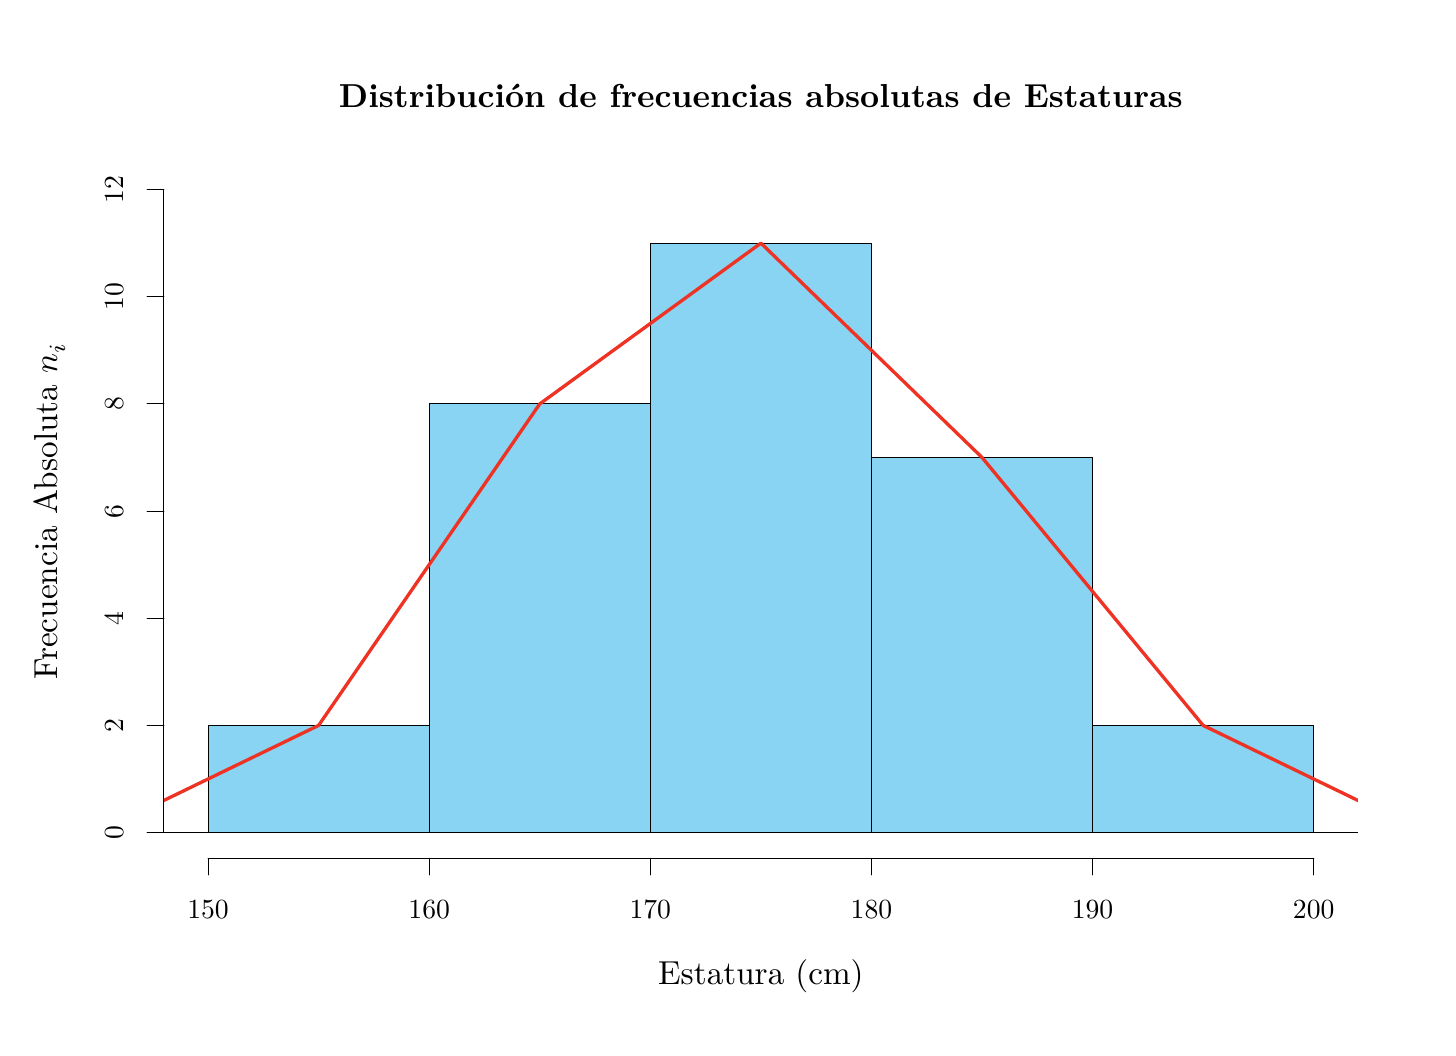
\begin{tikzpicture}[x=1pt,y=1pt]
\definecolor{fillColor}{RGB}{255,255,255}
\path[use as bounding box,fill=fillColor,fill opacity=0.00] (0,0) rectangle (505.89,361.35);
\begin{scope}
\path[clip] (  0.00,  0.00) rectangle (505.89,361.35);
\definecolor{drawColor}{RGB}{0,0,0}

\node[text=drawColor,anchor=base,inner sep=0pt, outer sep=0pt, scale=  1.20] at (264.95,332.61) {\bfseries Distribución de frecuencias absolutas de Estaturas};

\node[text=drawColor,anchor=base,inner sep=0pt, outer sep=0pt, scale=  1.20] at (264.95, 15.60) {Estatura (cm)};

\node[text=drawColor,rotate= 90.00,anchor=base,inner sep=0pt, outer sep=0pt, scale=  1.20] at ( 10.80,186.67) {Frecuencia Absoluta $n_i$};
\end{scope}
\begin{scope}
\path[clip] (  0.00,  0.00) rectangle (505.89,361.35);
\definecolor{drawColor}{RGB}{0,0,0}

\path[draw=drawColor,line width= 0.4pt,line join=round,line cap=round] ( 65.18, 61.20) -- (464.71, 61.20);

\path[draw=drawColor,line width= 0.4pt,line join=round,line cap=round] ( 65.18, 61.20) -- ( 65.18, 55.20);

\path[draw=drawColor,line width= 0.4pt,line join=round,line cap=round] (145.09, 61.20) -- (145.09, 55.20);

\path[draw=drawColor,line width= 0.4pt,line join=round,line cap=round] (224.99, 61.20) -- (224.99, 55.20);

\path[draw=drawColor,line width= 0.4pt,line join=round,line cap=round] (304.90, 61.20) -- (304.90, 55.20);

\path[draw=drawColor,line width= 0.4pt,line join=round,line cap=round] (384.80, 61.20) -- (384.80, 55.20);

\path[draw=drawColor,line width= 0.4pt,line join=round,line cap=round] (464.71, 61.20) -- (464.71, 55.20);

\node[text=drawColor,anchor=base,inner sep=0pt, outer sep=0pt, scale=  1.00] at ( 65.18, 39.60) {150};

\node[text=drawColor,anchor=base,inner sep=0pt, outer sep=0pt, scale=  1.00] at (145.09, 39.60) {160};

\node[text=drawColor,anchor=base,inner sep=0pt, outer sep=0pt, scale=  1.00] at (224.99, 39.60) {170};

\node[text=drawColor,anchor=base,inner sep=0pt, outer sep=0pt, scale=  1.00] at (304.90, 39.60) {180};

\node[text=drawColor,anchor=base,inner sep=0pt, outer sep=0pt, scale=  1.00] at (384.80, 39.60) {190};

\node[text=drawColor,anchor=base,inner sep=0pt, outer sep=0pt, scale=  1.00] at (464.71, 39.60) {200};

\path[draw=drawColor,line width= 0.4pt,line join=round,line cap=round] ( 49.20, 70.49) -- ( 49.20,302.86);

\path[draw=drawColor,line width= 0.4pt,line join=round,line cap=round] ( 49.20, 70.49) -- ( 43.20, 70.49);

\path[draw=drawColor,line width= 0.4pt,line join=round,line cap=round] ( 49.20,109.22) -- ( 43.20,109.22);

\path[draw=drawColor,line width= 0.4pt,line join=round,line cap=round] ( 49.20,147.95) -- ( 43.20,147.95);

\path[draw=drawColor,line width= 0.4pt,line join=round,line cap=round] ( 49.20,186.67) -- ( 43.20,186.67);

\path[draw=drawColor,line width= 0.4pt,line join=round,line cap=round] ( 49.20,225.40) -- ( 43.20,225.40);

\path[draw=drawColor,line width= 0.4pt,line join=round,line cap=round] ( 49.20,264.13) -- ( 43.20,264.13);

\path[draw=drawColor,line width= 0.4pt,line join=round,line cap=round] ( 49.20,302.86) -- ( 43.20,302.86);

\node[text=drawColor,rotate= 90.00,anchor=base,inner sep=0pt, outer sep=0pt, scale=  1.00] at ( 34.80, 70.49) {0};

\node[text=drawColor,rotate= 90.00,anchor=base,inner sep=0pt, outer sep=0pt, scale=  1.00] at ( 34.80,109.22) {2};

\node[text=drawColor,rotate= 90.00,anchor=base,inner sep=0pt, outer sep=0pt, scale=  1.00] at ( 34.80,147.95) {4};

\node[text=drawColor,rotate= 90.00,anchor=base,inner sep=0pt, outer sep=0pt, scale=  1.00] at ( 34.80,186.67) {6};

\node[text=drawColor,rotate= 90.00,anchor=base,inner sep=0pt, outer sep=0pt, scale=  1.00] at ( 34.80,225.40) {8};

\node[text=drawColor,rotate= 90.00,anchor=base,inner sep=0pt, outer sep=0pt, scale=  1.00] at ( 34.80,264.13) {10};

\node[text=drawColor,rotate= 90.00,anchor=base,inner sep=0pt, outer sep=0pt, scale=  1.00] at ( 34.80,302.86) {12};
\end{scope}
\begin{scope}
\path[clip] ( 49.20, 61.20) rectangle (480.69,312.15);
\definecolor{drawColor}{RGB}{0,0,0}
\definecolor{fillColor}{RGB}{137,211,243}

\path[draw=drawColor,line width= 0.4pt,line join=round,line cap=round,fill=fillColor] ( 65.18, 70.49) rectangle (145.09,109.22);

\path[draw=drawColor,line width= 0.4pt,line join=round,line cap=round,fill=fillColor] (145.09, 70.49) rectangle (224.99,225.40);

\path[draw=drawColor,line width= 0.4pt,line join=round,line cap=round,fill=fillColor] (224.99, 70.49) rectangle (304.90,283.49);

\path[draw=drawColor,line width= 0.4pt,line join=round,line cap=round,fill=fillColor] (304.90, 70.49) rectangle (384.80,206.04);

\path[draw=drawColor,line width= 0.4pt,line join=round,line cap=round,fill=fillColor] (384.80, 70.49) rectangle (464.71,109.22);
\definecolor{drawColor}{RGB}{238,50,36}

\path[draw=drawColor,line width= 1.2pt,line join=round,line cap=round] ( 25.23, 70.49) --
	(105.13,109.22) --
	(185.04,225.40) --
	(264.95,283.49) --
	(344.85,206.04) --
	(424.76,109.22) --
	(504.66, 70.49);
\definecolor{drawColor}{RGB}{0,0,0}

\path[draw=drawColor,line width= 0.4pt,line join=round,line cap=round] ( 49.20, 70.49) -- (480.69, 70.49);
\end{scope}
\end{tikzpicture}
}
\end{center}
\note{Al igual que para el diagra de barras, para el histograma también se puede construir el polígono de frecuencias
absolutas uniendo con segmentos los puntos más altos de cada barra sobre el centro del intervalo.}
\end{frame}


\mode<presentation>{
%---------------------------------------------------------------------slide----
\begin{frame}
\frametitle{Histograma de frecuencias absolutas acumuladas}
\framesubtitle{Datos agrupados}
\begin{center}
\tikzsetnextfilename{descriptiva/histograma_frecuencia_acumulada}
\scalebox{0.75}{%% Input file name: histograma_frecuencia_acumulada.fig
%% FIG version: 3.2
%% Orientation: Landscape
%% Justification: Flush Left
%% Units: Inches
%% Paper size: A4
%% Magnification: 100.0
%% Resolution: 1200ppi

\begin{pspicture}(6.70cm,3.48cm)(16.66cm,13.45cm)
\psset{unit=0.8cm}
%%
%% Depth: 2147483647
%%
\newrgbcolor{mycolor0}{1.00 0.50 0.31}\definecolor{mycolor0}{rgb}{1.00,0.50,0.31}
%%
%% Depth: 100
%%
%\rput(15.27,15.99){Histograma de frecuencias absolutas acumuladas}
\rput(15.27,4.86){Estatura}
\rput[l]{90}(8.89,7.61){Frecuencia absoluta acumulada $N_i$}
\psset{linestyle=solid,linewidth=0.03175,linecolor=black,fillstyle=none}
\psline(10.61,6.47)(19.94,6.47)
\psline(10.61,6.47)(10.61,6.26)
\psline(12.47,6.47)(12.47,6.26)
\psline(14.34,6.47)(14.34,6.26)
\psline(16.21,6.47)(16.21,6.26)
\psline(18.07,6.47)(18.07,6.26)
\psline(19.94,6.47)(19.94,6.26)
\rput(10.61,5.71){150}
\rput(12.47,5.71){160}
\rput(14.34,5.71){170}
\rput(16.21,5.71){180}
\rput(18.07,5.71){190}
\rput(19.94,5.71){200}
\psline(10.23,6.80)(10.23,14.95)
\psline(10.23,6.80)(10.02,6.80)
\psline(10.23,8.16)(10.02,8.16)
\psline(10.23,9.52)(10.02,9.52)
\psline(10.23,10.88)(10.02,10.88)
\psline(10.23,12.23)(10.02,12.23)
\psline(10.23,13.59)(10.02,13.59)
\psline(10.23,14.95)(10.02,14.95)
\rput{90}(9.73,6.80){0}
\rput{90}(9.73,8.16){5}
\rput{90}(9.73,9.52){10}
\rput{90}(9.73,10.88){15}
\rput{90}(9.73,12.23){20}
\rput{90}(9.73,13.59){25}
\rput{90}(9.73,14.95){30}
\psset{fillstyle=solid,fillcolor=mycolor0}
\pspolygon(10.61,6.80)(10.61,7.34)(12.47,7.34)(12.47,6.80)(10.61,6.80)
\pspolygon(12.47,6.80)(12.47,9.52)(14.34,9.52)(14.34,6.80)(12.47,6.80)
\pspolygon(14.34,6.80)(14.34,12.51)(16.21,12.51)(16.21,6.80)(14.34,6.80)
\pspolygon(16.21,6.80)(16.21,14.41)(18.07,14.41)(18.07,6.80)(16.21,6.80)
\pspolygon(18.07,6.80)(18.07,14.95)(19.94,14.95)(19.94,6.80)(18.07,6.80)
\end{pspicture}
%% End
}
\end{center}
\note{Este otro gráfico es el histograma de frecuencias absolutas acumuladas, en el que como puede apreciarse las
barras van creciendo progresivamente hasta alcanzar el tamaño de la muesta.}
\end{frame}


%---------------------------------------------------------------------slide----
\begin{frame}
\frametitle{Polígono de frecuencias absolutas acumuladas}
\framesubtitle{Datos agrupados}
\begin{center}
\tikzsetnextfilename{descriptiva/poligono_frecuencia_acumulada_agrupado}
\scalebox{0.6}{% Created by tikzDevice version 0.8.1 on 2015-11-09 19:49:49
% !TEX encoding = UTF-8 Unicode
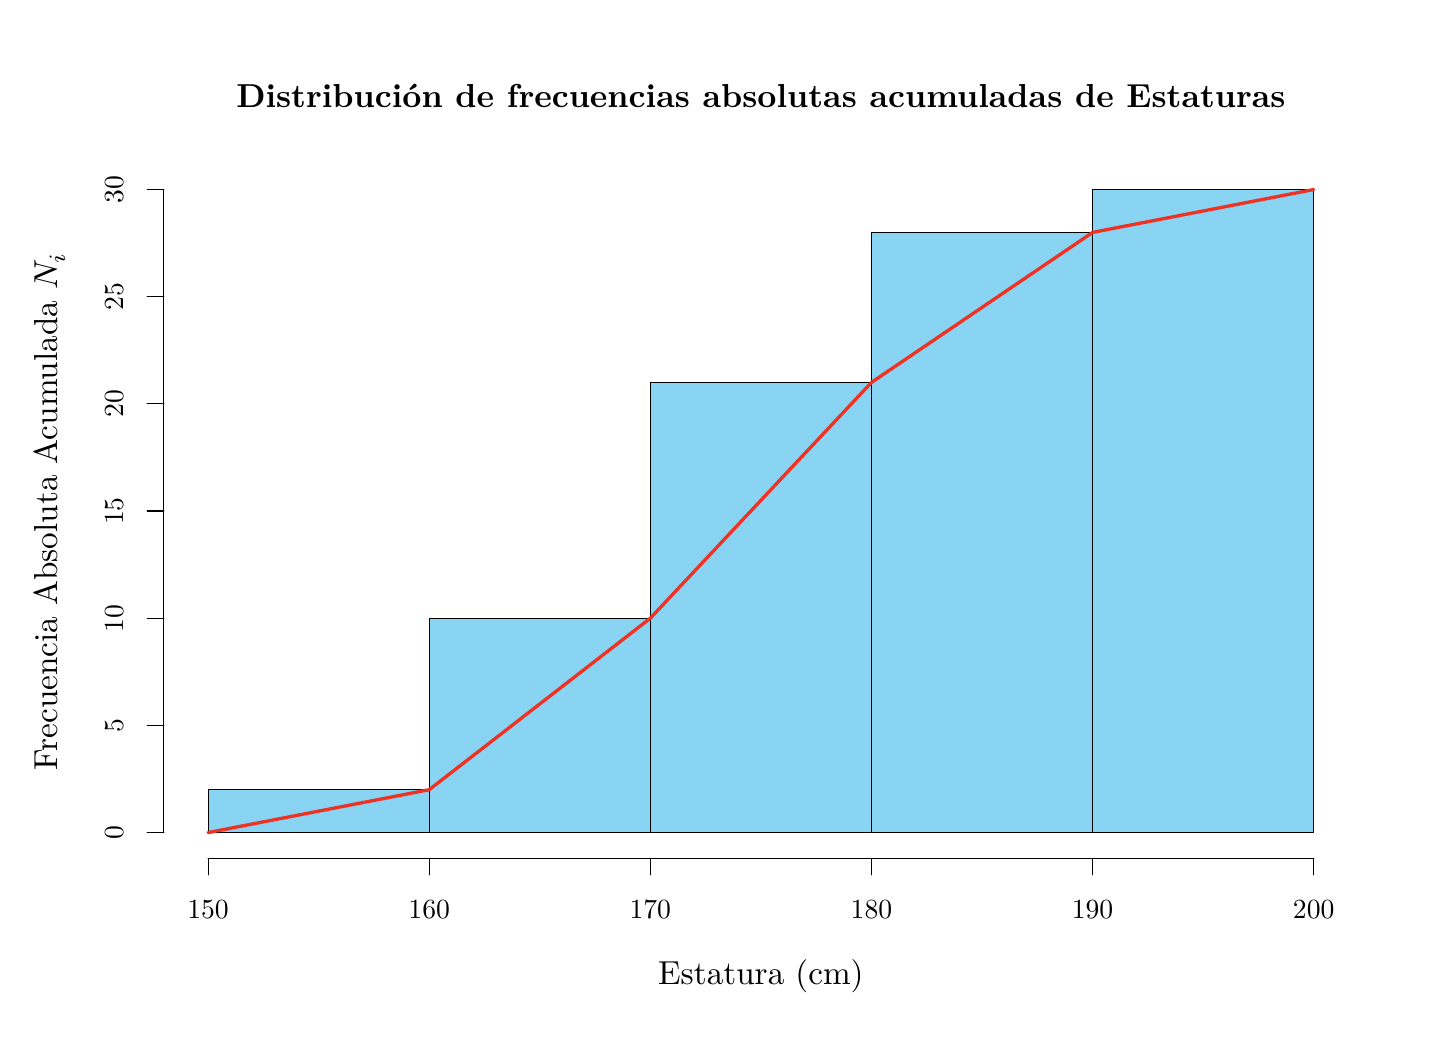
\begin{tikzpicture}[x=1pt,y=1pt]
\definecolor{fillColor}{RGB}{255,255,255}
\path[use as bounding box,fill=fillColor,fill opacity=0.00] (0,0) rectangle (505.89,361.35);
\begin{scope}
\path[clip] (  0.00,  0.00) rectangle (505.89,361.35);
\definecolor{drawColor}{RGB}{0,0,0}

\node[text=drawColor,anchor=base,inner sep=0pt, outer sep=0pt, scale=  1.20] at (264.95,332.61) {\bfseries Distribución de frecuencias absolutas acumuladas de Estaturas};

\node[text=drawColor,anchor=base,inner sep=0pt, outer sep=0pt, scale=  1.20] at (264.95, 15.60) {Estatura (cm)};

\node[text=drawColor,rotate= 90.00,anchor=base,inner sep=0pt, outer sep=0pt, scale=  1.20] at ( 10.80,186.67) {Frecuencia Absoluta Acumulada $N_i$};
\end{scope}
\begin{scope}
\path[clip] (  0.00,  0.00) rectangle (505.89,361.35);
\definecolor{drawColor}{RGB}{0,0,0}

\path[draw=drawColor,line width= 0.4pt,line join=round,line cap=round] ( 65.18, 61.20) -- (464.71, 61.20);

\path[draw=drawColor,line width= 0.4pt,line join=round,line cap=round] ( 65.18, 61.20) -- ( 65.18, 55.20);

\path[draw=drawColor,line width= 0.4pt,line join=round,line cap=round] (145.09, 61.20) -- (145.09, 55.20);

\path[draw=drawColor,line width= 0.4pt,line join=round,line cap=round] (224.99, 61.20) -- (224.99, 55.20);

\path[draw=drawColor,line width= 0.4pt,line join=round,line cap=round] (304.90, 61.20) -- (304.90, 55.20);

\path[draw=drawColor,line width= 0.4pt,line join=round,line cap=round] (384.80, 61.20) -- (384.80, 55.20);

\path[draw=drawColor,line width= 0.4pt,line join=round,line cap=round] (464.71, 61.20) -- (464.71, 55.20);

\node[text=drawColor,anchor=base,inner sep=0pt, outer sep=0pt, scale=  1.00] at ( 65.18, 39.60) {150};

\node[text=drawColor,anchor=base,inner sep=0pt, outer sep=0pt, scale=  1.00] at (145.09, 39.60) {160};

\node[text=drawColor,anchor=base,inner sep=0pt, outer sep=0pt, scale=  1.00] at (224.99, 39.60) {170};

\node[text=drawColor,anchor=base,inner sep=0pt, outer sep=0pt, scale=  1.00] at (304.90, 39.60) {180};

\node[text=drawColor,anchor=base,inner sep=0pt, outer sep=0pt, scale=  1.00] at (384.80, 39.60) {190};

\node[text=drawColor,anchor=base,inner sep=0pt, outer sep=0pt, scale=  1.00] at (464.71, 39.60) {200};

\path[draw=drawColor,line width= 0.4pt,line join=round,line cap=round] ( 49.20, 70.49) -- ( 49.20,302.86);

\path[draw=drawColor,line width= 0.4pt,line join=round,line cap=round] ( 49.20, 70.49) -- ( 43.20, 70.49);

\path[draw=drawColor,line width= 0.4pt,line join=round,line cap=round] ( 49.20,109.22) -- ( 43.20,109.22);

\path[draw=drawColor,line width= 0.4pt,line join=round,line cap=round] ( 49.20,147.95) -- ( 43.20,147.95);

\path[draw=drawColor,line width= 0.4pt,line join=round,line cap=round] ( 49.20,186.68) -- ( 43.20,186.68);

\path[draw=drawColor,line width= 0.4pt,line join=round,line cap=round] ( 49.20,225.40) -- ( 43.20,225.40);

\path[draw=drawColor,line width= 0.4pt,line join=round,line cap=round] ( 49.20,264.13) -- ( 43.20,264.13);

\path[draw=drawColor,line width= 0.4pt,line join=round,line cap=round] ( 49.20,302.86) -- ( 43.20,302.86);

\node[text=drawColor,rotate= 90.00,anchor=base,inner sep=0pt, outer sep=0pt, scale=  1.00] at ( 34.80, 70.49) {0};

\node[text=drawColor,rotate= 90.00,anchor=base,inner sep=0pt, outer sep=0pt, scale=  1.00] at ( 34.80,109.22) {5};

\node[text=drawColor,rotate= 90.00,anchor=base,inner sep=0pt, outer sep=0pt, scale=  1.00] at ( 34.80,147.95) {10};

\node[text=drawColor,rotate= 90.00,anchor=base,inner sep=0pt, outer sep=0pt, scale=  1.00] at ( 34.80,186.68) {15};

\node[text=drawColor,rotate= 90.00,anchor=base,inner sep=0pt, outer sep=0pt, scale=  1.00] at ( 34.80,225.40) {20};

\node[text=drawColor,rotate= 90.00,anchor=base,inner sep=0pt, outer sep=0pt, scale=  1.00] at ( 34.80,264.13) {25};

\node[text=drawColor,rotate= 90.00,anchor=base,inner sep=0pt, outer sep=0pt, scale=  1.00] at ( 34.80,302.86) {30};
\end{scope}
\begin{scope}
\path[clip] ( 49.20, 61.20) rectangle (480.69,312.15);
\definecolor{drawColor}{RGB}{0,0,0}
\definecolor{fillColor}{RGB}{137,211,243}

\path[draw=drawColor,line width= 0.4pt,line join=round,line cap=round,fill=fillColor] ( 65.18, 70.49) rectangle (145.09, 85.99);

\path[draw=drawColor,line width= 0.4pt,line join=round,line cap=round,fill=fillColor] (145.09, 70.49) rectangle (224.99,147.95);

\path[draw=drawColor,line width= 0.4pt,line join=round,line cap=round,fill=fillColor] (224.99, 70.49) rectangle (304.90,233.15);

\path[draw=drawColor,line width= 0.4pt,line join=round,line cap=round,fill=fillColor] (304.90, 70.49) rectangle (384.80,287.36);

\path[draw=drawColor,line width= 0.4pt,line join=round,line cap=round,fill=fillColor] (384.80, 70.49) rectangle (464.71,302.86);
\definecolor{drawColor}{RGB}{238,50,36}

\path[draw=drawColor,line width= 1.2pt,line join=round,line cap=round] ( 65.18, 70.49) --
	(145.09, 85.99) --
	(224.99,147.95) --
	(304.90,233.15) --
	(384.80,287.36) --
	(464.71,302.86);
\end{scope}
\end{tikzpicture}
}
\end{center}
\note{En el caso de histogramas de frecuencias acumuladas, el polígono correspondiente se construye mediante segmentos
que unen el vértice inferior izquierdo y el vértice superior derecho de cada barra, reflejando, a diferencia del
polígono de frecuencias acumuladas del diagrama de barras que tenía forma de escalera, que la acumulación de individuos
es progresiva a medida que se recorre el intervalo.}
\end{frame}
}

%---------------------------------------------------------------------slide----
\begin{frame}
\frametitle{Histograma de frecuencias relativas acumuladas}
\framesubtitle{Datos agrupados}
\begin{center}
\tikzsetnextfilename{descriptiva/histograma_frecuencia_relativa_acumulada_agrupado}
\scalebox{0.6}{% Created by tikzDevice version 0.8.1 on 2015-11-09 19:55:17
% !TEX encoding = UTF-8 Unicode
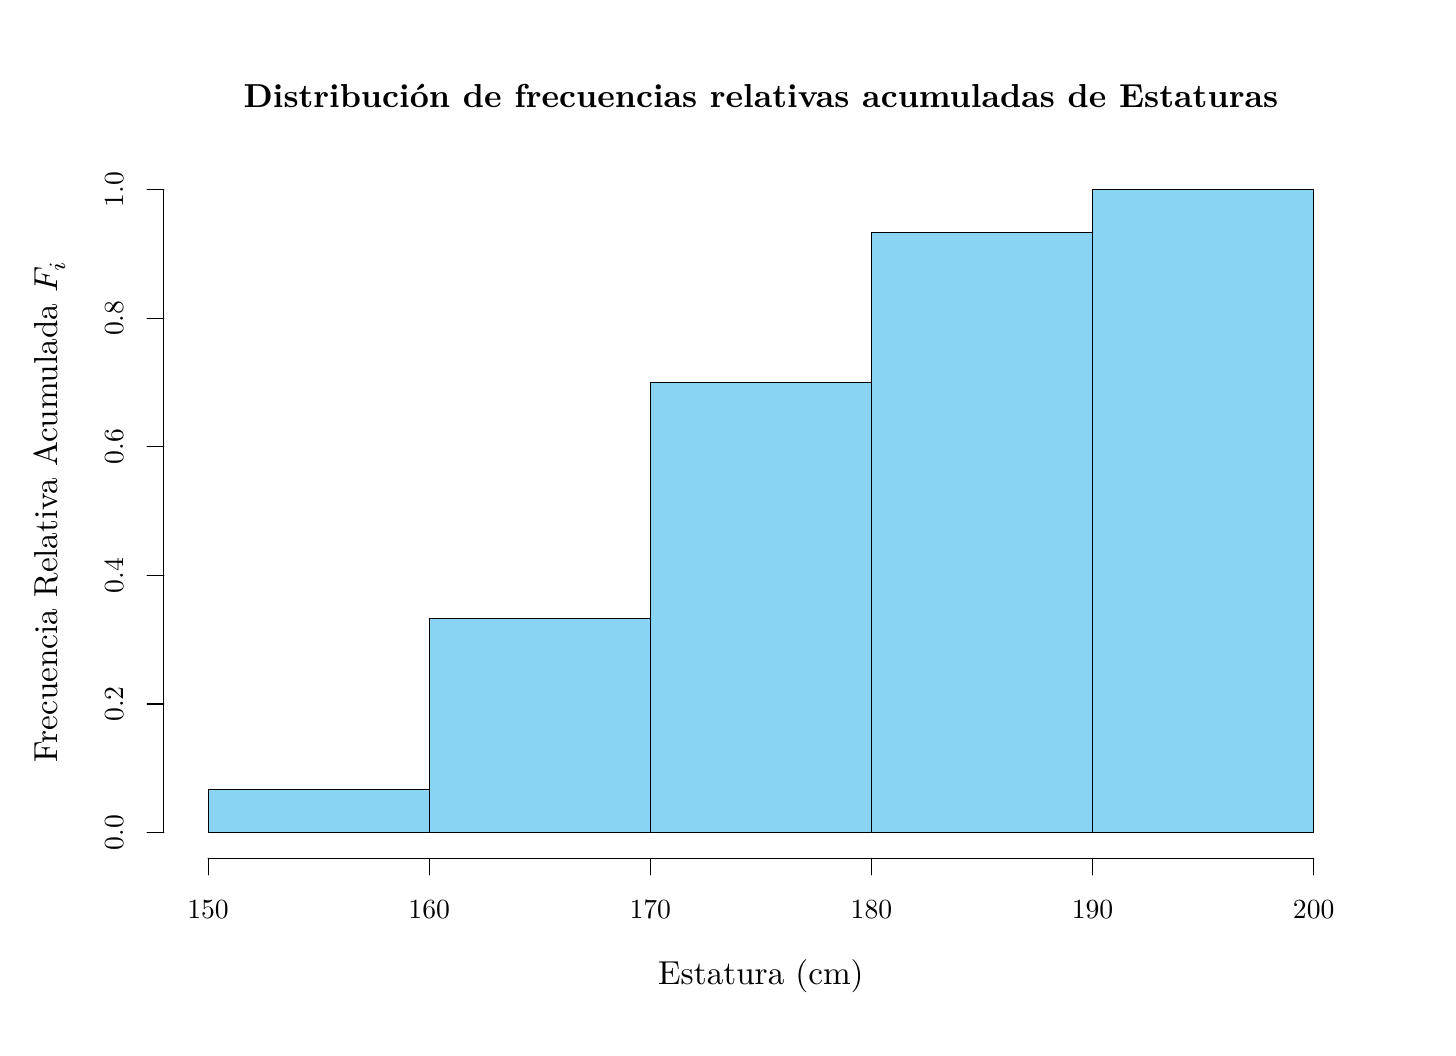
\begin{tikzpicture}[x=1pt,y=1pt]
\definecolor{fillColor}{RGB}{255,255,255}
\path[use as bounding box,fill=fillColor,fill opacity=0.00] (0,0) rectangle (505.89,361.35);
\begin{scope}
\path[clip] (  0.00,  0.00) rectangle (505.89,361.35);
\definecolor{drawColor}{RGB}{0,0,0}

\node[text=drawColor,anchor=base,inner sep=0pt, outer sep=0pt, scale=  1.20] at (264.95,332.61) {\bfseries Distribución de frecuencias relativas acumuladas de Estaturas};

\node[text=drawColor,anchor=base,inner sep=0pt, outer sep=0pt, scale=  1.20] at (264.95, 15.60) {Estatura (cm)};

\node[text=drawColor,rotate= 90.00,anchor=base,inner sep=0pt, outer sep=0pt, scale=  1.20] at ( 10.80,186.67) {Frecuencia Relativa Acumulada $F_i$};
\end{scope}
\begin{scope}
\path[clip] (  0.00,  0.00) rectangle (505.89,361.35);
\definecolor{drawColor}{RGB}{0,0,0}

\path[draw=drawColor,line width= 0.4pt,line join=round,line cap=round] ( 65.18, 61.20) -- (464.71, 61.20);

\path[draw=drawColor,line width= 0.4pt,line join=round,line cap=round] ( 65.18, 61.20) -- ( 65.18, 55.20);

\path[draw=drawColor,line width= 0.4pt,line join=round,line cap=round] (145.09, 61.20) -- (145.09, 55.20);

\path[draw=drawColor,line width= 0.4pt,line join=round,line cap=round] (224.99, 61.20) -- (224.99, 55.20);

\path[draw=drawColor,line width= 0.4pt,line join=round,line cap=round] (304.90, 61.20) -- (304.90, 55.20);

\path[draw=drawColor,line width= 0.4pt,line join=round,line cap=round] (384.80, 61.20) -- (384.80, 55.20);

\path[draw=drawColor,line width= 0.4pt,line join=round,line cap=round] (464.71, 61.20) -- (464.71, 55.20);

\node[text=drawColor,anchor=base,inner sep=0pt, outer sep=0pt, scale=  1.00] at ( 65.18, 39.60) {150};

\node[text=drawColor,anchor=base,inner sep=0pt, outer sep=0pt, scale=  1.00] at (145.09, 39.60) {160};

\node[text=drawColor,anchor=base,inner sep=0pt, outer sep=0pt, scale=  1.00] at (224.99, 39.60) {170};

\node[text=drawColor,anchor=base,inner sep=0pt, outer sep=0pt, scale=  1.00] at (304.90, 39.60) {180};

\node[text=drawColor,anchor=base,inner sep=0pt, outer sep=0pt, scale=  1.00] at (384.80, 39.60) {190};

\node[text=drawColor,anchor=base,inner sep=0pt, outer sep=0pt, scale=  1.00] at (464.71, 39.60) {200};

\path[draw=drawColor,line width= 0.4pt,line join=round,line cap=round] ( 49.20, 70.49) -- ( 49.20,302.86);

\path[draw=drawColor,line width= 0.4pt,line join=round,line cap=round] ( 49.20, 70.49) -- ( 43.20, 70.49);

\path[draw=drawColor,line width= 0.4pt,line join=round,line cap=round] ( 49.20,116.97) -- ( 43.20,116.97);

\path[draw=drawColor,line width= 0.4pt,line join=round,line cap=round] ( 49.20,163.44) -- ( 43.20,163.44);

\path[draw=drawColor,line width= 0.4pt,line join=round,line cap=round] ( 49.20,209.91) -- ( 43.20,209.91);

\path[draw=drawColor,line width= 0.4pt,line join=round,line cap=round] ( 49.20,256.38) -- ( 43.20,256.38);

\path[draw=drawColor,line width= 0.4pt,line join=round,line cap=round] ( 49.20,302.86) -- ( 43.20,302.86);

\node[text=drawColor,rotate= 90.00,anchor=base,inner sep=0pt, outer sep=0pt, scale=  1.00] at ( 34.80, 70.49) {0.0};

\node[text=drawColor,rotate= 90.00,anchor=base,inner sep=0pt, outer sep=0pt, scale=  1.00] at ( 34.80,116.97) {0.2};

\node[text=drawColor,rotate= 90.00,anchor=base,inner sep=0pt, outer sep=0pt, scale=  1.00] at ( 34.80,163.44) {0.4};

\node[text=drawColor,rotate= 90.00,anchor=base,inner sep=0pt, outer sep=0pt, scale=  1.00] at ( 34.80,209.91) {0.6};

\node[text=drawColor,rotate= 90.00,anchor=base,inner sep=0pt, outer sep=0pt, scale=  1.00] at ( 34.80,256.38) {0.8};

\node[text=drawColor,rotate= 90.00,anchor=base,inner sep=0pt, outer sep=0pt, scale=  1.00] at ( 34.80,302.86) {1.0};
\end{scope}
\begin{scope}
\path[clip] ( 49.20, 61.20) rectangle (480.69,312.15);
\definecolor{drawColor}{RGB}{0,0,0}
\definecolor{fillColor}{RGB}{137,211,243}

\path[draw=drawColor,line width= 0.4pt,line join=round,line cap=round,fill=fillColor] ( 65.18, 70.49) rectangle (145.09, 85.99);

\path[draw=drawColor,line width= 0.4pt,line join=round,line cap=round,fill=fillColor] (145.09, 70.49) rectangle (224.99,147.95);

\path[draw=drawColor,line width= 0.4pt,line join=round,line cap=round,fill=fillColor] (224.99, 70.49) rectangle (304.90,233.15);

\path[draw=drawColor,line width= 0.4pt,line join=round,line cap=round,fill=fillColor] (304.90, 70.49) rectangle (384.80,287.36);

\path[draw=drawColor,line width= 0.4pt,line join=round,line cap=round,fill=fillColor] (384.80, 70.49) rectangle (464.71,302.86);
\end{scope}
\end{tikzpicture}
}
\end{center} 
\end{frame}


%---------------------------------------------------------------------slide----
\begin{frame}
\frametitle{Polígono de frecuencias relativas acumuladas}
\framesubtitle{Datos agrupados}
\begin{center}
\tikzsetnextfilename{descriptiva/poligono_frecuencia_relativa_acumulada_agrupado}
\scalebox{0.6}{% Created by tikzDevice version 0.8.1 on 2015-11-09 19:55:17
% !TEX encoding = UTF-8 Unicode
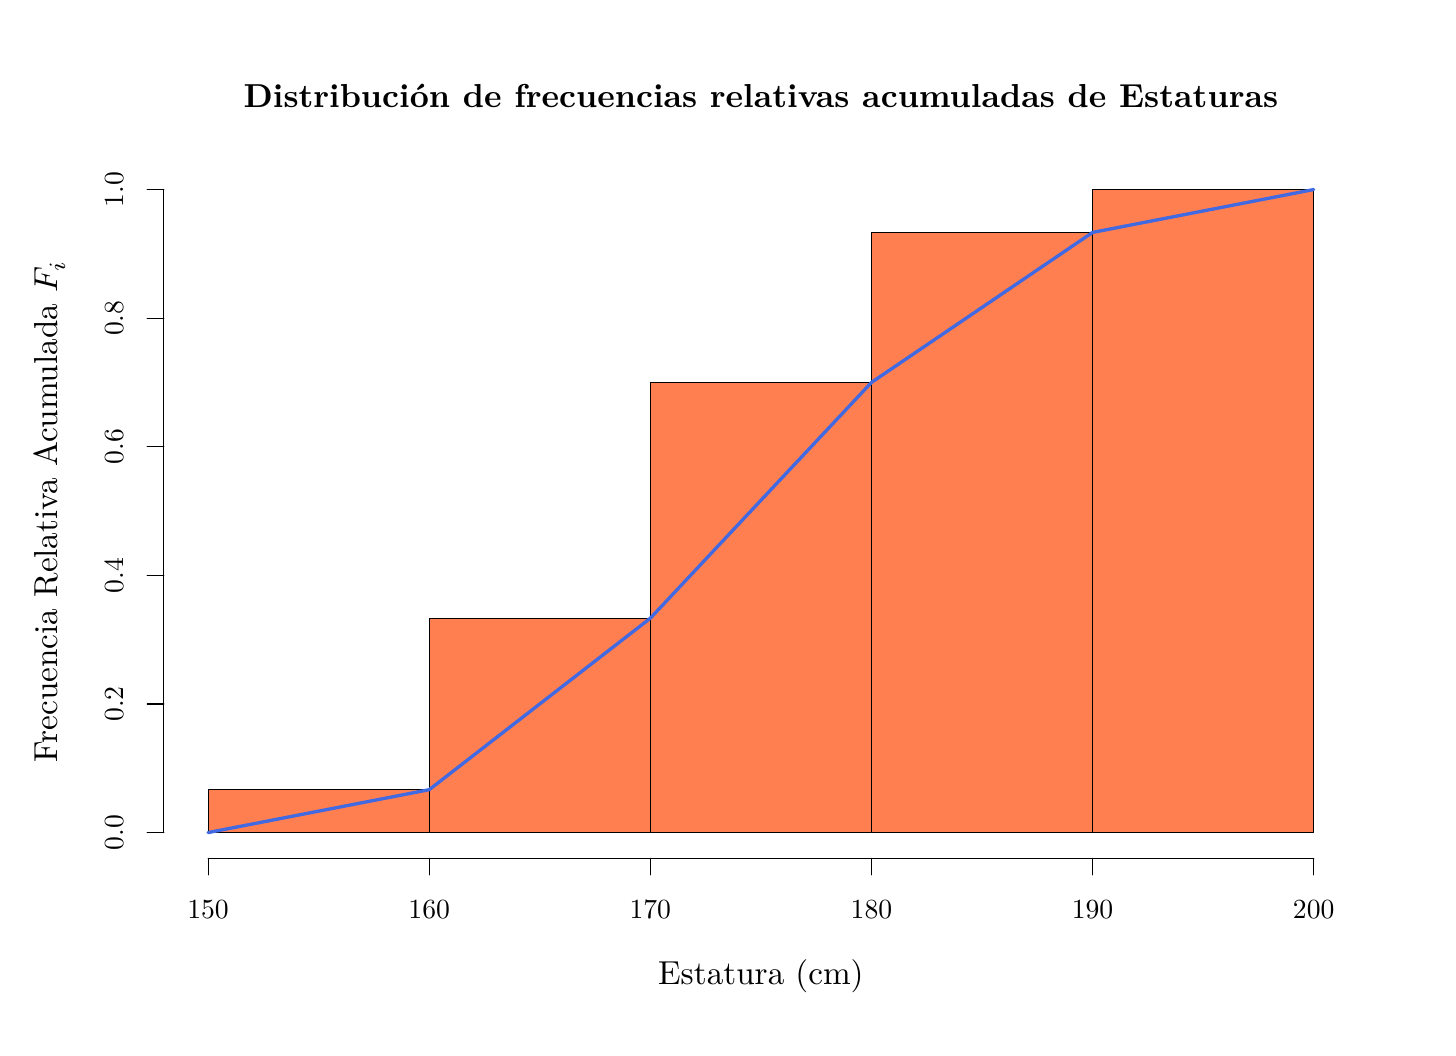
\begin{tikzpicture}[x=1pt,y=1pt]
\definecolor{fillColor}{RGB}{255,255,255}
\path[use as bounding box,fill=fillColor,fill opacity=0.00] (0,0) rectangle (505.89,361.35);
\begin{scope}
\path[clip] (  0.00,  0.00) rectangle (505.89,361.35);
\definecolor{drawColor}{RGB}{0,0,0}

\node[text=drawColor,anchor=base,inner sep=0pt, outer sep=0pt, scale=  1.20] at (264.95,332.61) {\bfseries Distribución de frecuencias relativas acumuladas de Estaturas};

\node[text=drawColor,anchor=base,inner sep=0pt, outer sep=0pt, scale=  1.20] at (264.95, 15.60) {Estatura (cm)};

\node[text=drawColor,rotate= 90.00,anchor=base,inner sep=0pt, outer sep=0pt, scale=  1.20] at ( 10.80,186.67) {Frecuencia Relativa Acumulada $F_i$};
\end{scope}
\begin{scope}
\path[clip] (  0.00,  0.00) rectangle (505.89,361.35);
\definecolor{drawColor}{RGB}{0,0,0}

\path[draw=drawColor,line width= 0.4pt,line join=round,line cap=round] ( 65.18, 61.20) -- (464.71, 61.20);

\path[draw=drawColor,line width= 0.4pt,line join=round,line cap=round] ( 65.18, 61.20) -- ( 65.18, 55.20);

\path[draw=drawColor,line width= 0.4pt,line join=round,line cap=round] (145.09, 61.20) -- (145.09, 55.20);

\path[draw=drawColor,line width= 0.4pt,line join=round,line cap=round] (224.99, 61.20) -- (224.99, 55.20);

\path[draw=drawColor,line width= 0.4pt,line join=round,line cap=round] (304.90, 61.20) -- (304.90, 55.20);

\path[draw=drawColor,line width= 0.4pt,line join=round,line cap=round] (384.80, 61.20) -- (384.80, 55.20);

\path[draw=drawColor,line width= 0.4pt,line join=round,line cap=round] (464.71, 61.20) -- (464.71, 55.20);

\node[text=drawColor,anchor=base,inner sep=0pt, outer sep=0pt, scale=  1.00] at ( 65.18, 39.60) {150};

\node[text=drawColor,anchor=base,inner sep=0pt, outer sep=0pt, scale=  1.00] at (145.09, 39.60) {160};

\node[text=drawColor,anchor=base,inner sep=0pt, outer sep=0pt, scale=  1.00] at (224.99, 39.60) {170};

\node[text=drawColor,anchor=base,inner sep=0pt, outer sep=0pt, scale=  1.00] at (304.90, 39.60) {180};

\node[text=drawColor,anchor=base,inner sep=0pt, outer sep=0pt, scale=  1.00] at (384.80, 39.60) {190};

\node[text=drawColor,anchor=base,inner sep=0pt, outer sep=0pt, scale=  1.00] at (464.71, 39.60) {200};

\path[draw=drawColor,line width= 0.4pt,line join=round,line cap=round] ( 49.20, 70.49) -- ( 49.20,302.86);

\path[draw=drawColor,line width= 0.4pt,line join=round,line cap=round] ( 49.20, 70.49) -- ( 43.20, 70.49);

\path[draw=drawColor,line width= 0.4pt,line join=round,line cap=round] ( 49.20,116.97) -- ( 43.20,116.97);

\path[draw=drawColor,line width= 0.4pt,line join=round,line cap=round] ( 49.20,163.44) -- ( 43.20,163.44);

\path[draw=drawColor,line width= 0.4pt,line join=round,line cap=round] ( 49.20,209.91) -- ( 43.20,209.91);

\path[draw=drawColor,line width= 0.4pt,line join=round,line cap=round] ( 49.20,256.38) -- ( 43.20,256.38);

\path[draw=drawColor,line width= 0.4pt,line join=round,line cap=round] ( 49.20,302.86) -- ( 43.20,302.86);

\node[text=drawColor,rotate= 90.00,anchor=base,inner sep=0pt, outer sep=0pt, scale=  1.00] at ( 34.80, 70.49) {0.0};

\node[text=drawColor,rotate= 90.00,anchor=base,inner sep=0pt, outer sep=0pt, scale=  1.00] at ( 34.80,116.97) {0.2};

\node[text=drawColor,rotate= 90.00,anchor=base,inner sep=0pt, outer sep=0pt, scale=  1.00] at ( 34.80,163.44) {0.4};

\node[text=drawColor,rotate= 90.00,anchor=base,inner sep=0pt, outer sep=0pt, scale=  1.00] at ( 34.80,209.91) {0.6};

\node[text=drawColor,rotate= 90.00,anchor=base,inner sep=0pt, outer sep=0pt, scale=  1.00] at ( 34.80,256.38) {0.8};

\node[text=drawColor,rotate= 90.00,anchor=base,inner sep=0pt, outer sep=0pt, scale=  1.00] at ( 34.80,302.86) {1.0};
\end{scope}
\begin{scope}
\path[clip] ( 49.20, 61.20) rectangle (480.69,312.15);
\definecolor{drawColor}{RGB}{0,0,0}
\definecolor{fillColor}{RGB}{255,127,80}

\path[draw=drawColor,line width= 0.4pt,line join=round,line cap=round,fill=fillColor] ( 65.18, 70.49) rectangle (145.09, 85.99);

\path[draw=drawColor,line width= 0.4pt,line join=round,line cap=round,fill=fillColor] (145.09, 70.49) rectangle (224.99,147.95);

\path[draw=drawColor,line width= 0.4pt,line join=round,line cap=round,fill=fillColor] (224.99, 70.49) rectangle (304.90,233.15);

\path[draw=drawColor,line width= 0.4pt,line join=round,line cap=round,fill=fillColor] (304.90, 70.49) rectangle (384.80,287.36);

\path[draw=drawColor,line width= 0.4pt,line join=round,line cap=round,fill=fillColor] (384.80, 70.49) rectangle (464.71,302.86);
\definecolor{drawColor}{RGB}{65,105,225}

\path[draw=drawColor,line width= 1.2pt,line join=round,line cap=round] ( 65.18, 70.49) --
	(145.09, 85.99) --
	(224.99,147.95) --
	(304.90,233.15) --
	(384.80,287.36) --
	(464.71,302.86);
\end{scope}
\end{tikzpicture}
} 
\end{center} 
\end{frame}
\mode<article>
{El polígono de frecuencias acumuladas (absolutas o relativas) se conoce como \textbf{ojiva}.

Observese que en la ojiva se unen con segmentos los vértices superiores derechos de cada barra, en lugar de los centros, ya que no se consigue acumalar la correspondiente frecuencia hasta el final del intervalo.}


%---------------------------------------------------------------------slide----
\begin{frame}
\frametitle{Diagrama de sectores}
Un \highlight{diagrama de sectores} consiste en un círculo divido en porciones, uno por cada valor o categoría de la variable.

Cada porción se conoce como \highlight{sector} y su ángulo o área es proporcional a la correspondiente frecuencia del valor o categoría.

Los diagramas de sectores pueden representar frecuencias absolutas o relativas, pero no pueden representar frecuencias acumuladas, y se utilizan sobre todo con atributos nominales.
Para atributos ordinales o variables cuantitativas es mejor utilizar diagramas de barras o histogramas, ya es más fácil percibir las diferencias en una dimensión (altura de las barras) que en dos dimensiones (áreas de los sectores).
\end{frame}


%---------------------------------------------------------------------slide----
\begin{frame}
\frametitle{Diagrama de sectores}
\framesubtitle{Atributos}
\begin{center}
\tikzsetnextfilename{descriptiva/diagrama_sectores_frecuencia_relativa}
\scalebox{0.6}{% Created by tikzDevice version 0.8.1 on 2015-11-09 20:32:18
% !TEX encoding = UTF-8 Unicode
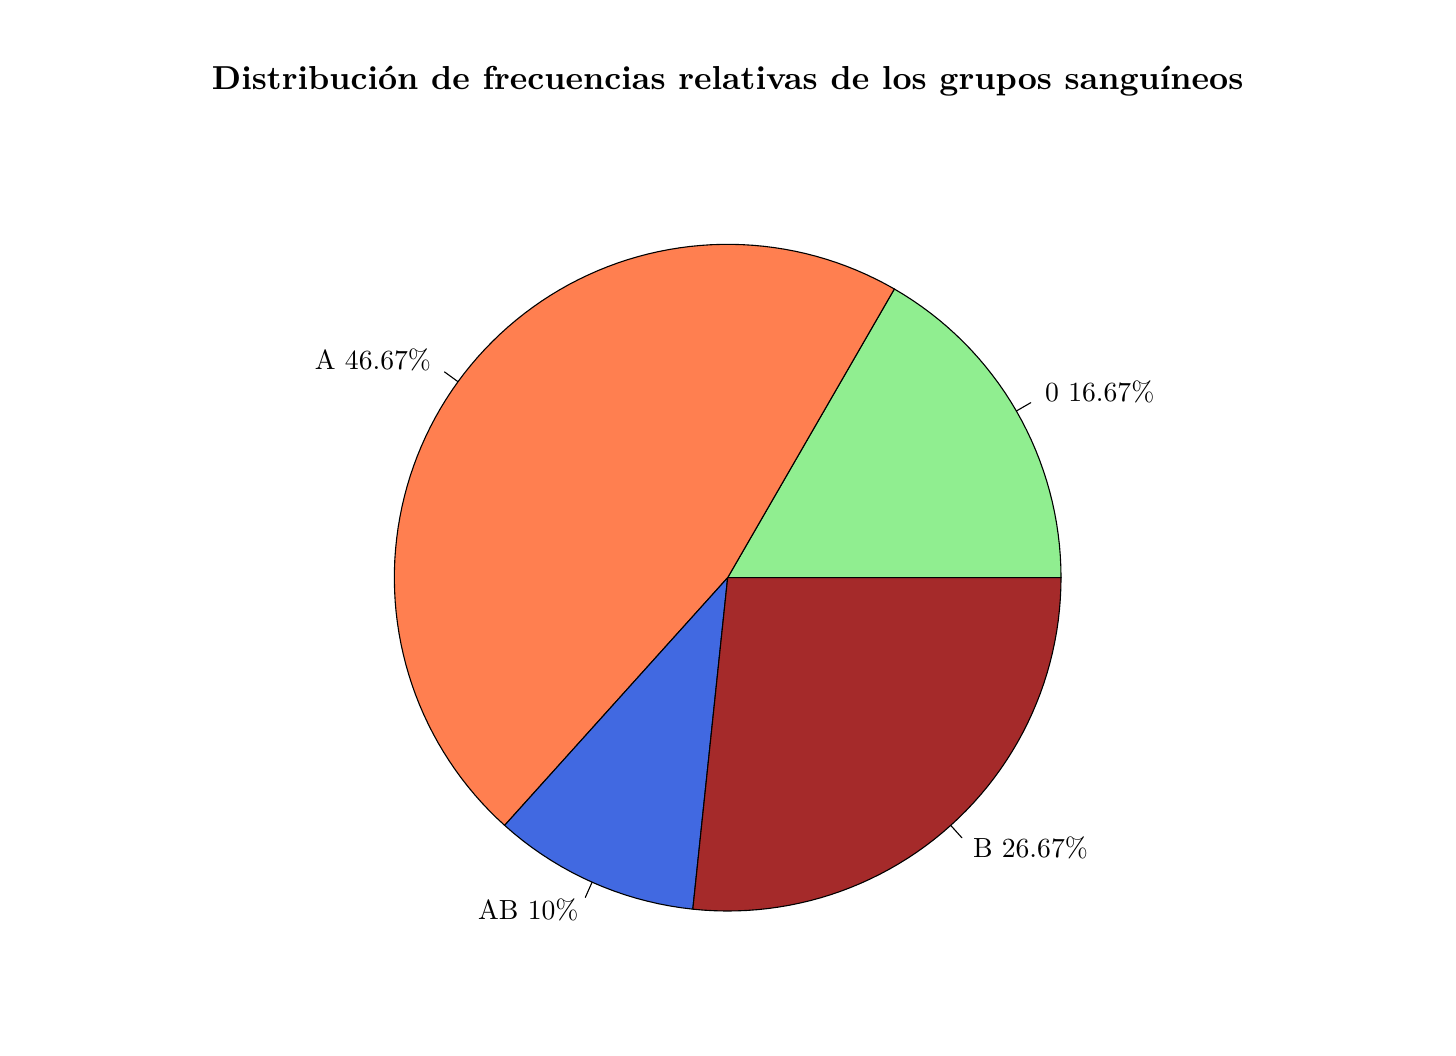
\begin{tikzpicture}[x=1pt,y=1pt]
\definecolor{fillColor}{RGB}{255,255,255}
\path[use as bounding box,fill=fillColor,fill opacity=0.00] (0,0) rectangle (505.89,361.35);
\begin{scope}
\path[clip] (  0.00,  0.00) rectangle (505.89,325.21);
\definecolor{drawColor}{RGB}{0,0,0}
\definecolor{fillColor}{RGB}{144,238,144}

\path[draw=drawColor,line width= 0.4pt,line join=round,line cap=round,fill=fillColor] (373.40,162.61) --
	(373.33,166.55) --
	(373.14,170.49) --
	(372.82,174.41) --
	(372.36,178.33) --
	(371.79,182.23) --
	(371.08,186.11) --
	(370.25,189.96) --
	(369.29,193.78) --
	(368.21,197.57) --
	(367.00,201.32) --
	(365.67,205.04) --
	(364.23,208.70) --
	(362.66,212.32) --
	(360.97,215.88) --
	(359.17,219.39) --
	(357.26,222.83) --
	(355.23,226.21) --
	(353.10,229.53) --
	(350.85,232.77) --
	(348.50,235.93) --
	(346.05,239.02) --
	(343.50,242.03) --
	(340.86,244.95) --
	(338.12,247.78) --
	(335.28,250.52) --
	(332.36,253.17) --
	(329.36,255.72) --
	(326.27,258.17) --
	(323.10,260.51) --
	(319.86,262.76) --
	(316.55,264.89) --
	(313.17,266.92) --
	(252.94,162.61) --
	cycle;

\path[draw=drawColor,line width= 0.4pt,line join=round,line cap=round] (357.26,222.83) --
	(362.47,225.84);
\end{scope}
\begin{scope}
\path[clip] (  0.00,  0.00) rectangle (505.89,361.35);
\definecolor{drawColor}{RGB}{0,0,0}

\node[text=drawColor,anchor=base west,inner sep=0pt, outer sep=0pt, scale=  1.00] at (367.69,226.36) {0 16.67\%};
\end{scope}
\begin{scope}
\path[clip] (  0.00,  0.00) rectangle (505.89,325.21);
\definecolor{drawColor}{RGB}{0,0,0}
\definecolor{fillColor}{RGB}{255,127,80}

\path[draw=drawColor,line width= 0.4pt,line join=round,line cap=round,fill=fillColor] (313.17,266.92) --
	(309.82,268.79) --
	(306.40,270.54) --
	(302.94,272.19) --
	(299.42,273.73) --
	(295.85,275.16) --
	(292.25,276.47) --
	(288.60,277.66) --
	(284.91,278.74) --
	(281.20,279.70) --
	(277.45,280.54) --
	(273.68,281.26) --
	(269.89,281.86) --
	(266.08,282.34) --
	(262.26,282.70) --
	(258.43,282.93) --
	(254.59,283.05) --
	(250.75,283.04) --
	(246.91,282.91) --
	(243.08,282.65) --
	(239.26,282.28) --
	(235.46,281.78) --
	(231.67,281.16) --
	(227.90,280.43) --
	(224.16,279.57) --
	(220.45,278.59) --
	(216.77,277.50) --
	(213.13,276.29) --
	(209.52,274.96) --
	(205.97,273.52) --
	(202.46,271.96) --
	(199.00,270.30) --
	(195.59,268.53) --
	(192.25,266.64) --
	(188.96,264.66) --
	(185.74,262.57) --
	(182.59,260.37) --
	(179.51,258.08) --
	(176.51,255.69) --
	(173.58,253.21) --
	(170.73,250.64) --
	(167.97,247.97) --
	(165.29,245.22) --
	(162.70,242.39) --
	(160.21,239.47) --
	(157.80,236.48) --
	(155.50,233.41) --
	(153.29,230.27) --
	(151.19,227.06) --
	(149.18,223.78) --
	(147.29,220.44) --
	(145.50,217.05) --
	(143.82,213.59) --
	(142.25,210.09) --
	(140.79,206.54) --
	(139.45,202.94) --
	(138.22,199.31) --
	(137.11,195.63) --
	(136.12,191.92) --
	(135.24,188.19) --
	(134.49,184.42) --
	(133.85,180.64) --
	(133.34,176.83) --
	(132.95,173.01) --
	(132.67,169.19) --
	(132.53,165.35) --
	(132.50,161.51) --
	(132.60,157.67) --
	(132.81,153.84) --
	(133.15,150.02) --
	(133.62,146.21) --
	(134.20,142.41) --
	(134.90,138.64) --
	(135.73,134.89) --
	(136.67,131.17) --
	(137.73,127.48) --
	(138.91,123.83) --
	(140.20,120.21) --
	(141.61,116.64) --
	(143.13,113.12) --
	(144.77,109.64) --
	(146.51,106.22) --
	(148.36,102.86) --
	(150.32, 99.56) --
	(152.38, 96.32) --
	(154.54, 93.15) --
	(156.80, 90.05) --
	(159.17, 87.02) --
	(161.62, 84.07) --
	(164.17, 81.20) --
	(166.81, 78.41) --
	(169.54, 75.71) --
	(172.35, 73.10) --
	(252.94,162.61) --
	cycle;

\path[draw=drawColor,line width= 0.4pt,line join=round,line cap=round] (155.50,233.41) --
	(150.63,236.95);
\end{scope}
\begin{scope}
\path[clip] (  0.00,  0.00) rectangle (505.89,361.35);
\definecolor{drawColor}{RGB}{0,0,0}

\node[text=drawColor,anchor=base east,inner sep=0pt, outer sep=0pt, scale=  1.00] at (145.75,237.99) {A 46.67\%};
\end{scope}
\begin{scope}
\path[clip] (  0.00,  0.00) rectangle (505.89,325.21);
\definecolor{drawColor}{RGB}{0,0,0}
\definecolor{fillColor}{RGB}{65,105,225}

\path[draw=drawColor,line width= 0.4pt,line join=round,line cap=round,fill=fillColor] (172.35, 73.10) --
	(175.52, 70.34) --
	(178.79, 67.69) --
	(182.15, 65.16) --
	(185.59, 62.75) --
	(189.12, 60.46) --
	(192.72, 58.29) --
	(196.40, 56.26) --
	(200.14, 54.35) --
	(203.95, 52.57) --
	(207.82, 50.93) --
	(211.75, 49.42) --
	(215.72, 48.05) --
	(219.74, 46.82) --
	(223.81, 45.74) --
	(227.90, 44.79) --
	(232.03, 43.99) --
	(236.18, 43.33) --
	(240.35, 42.82) --
	(252.94,162.61) --
	cycle;

\path[draw=drawColor,line width= 0.4pt,line join=round,line cap=round] (203.95, 52.57) --
	(201.50, 47.07);
\end{scope}
\begin{scope}
\path[clip] (  0.00,  0.00) rectangle (505.89,361.35);
\definecolor{drawColor}{RGB}{0,0,0}

\node[text=drawColor,anchor=base east,inner sep=0pt, outer sep=0pt, scale=  1.00] at (199.05, 39.07) {AB 10\%};
\end{scope}
\begin{scope}
\path[clip] (  0.00,  0.00) rectangle (505.89,325.21);
\definecolor{drawColor}{RGB}{0,0,0}
\definecolor{fillColor}{RGB}{165,42,42}

\path[draw=drawColor,line width= 0.4pt,line join=round,line cap=round,fill=fillColor] (240.35, 42.82) --
	(244.22, 42.47) --
	(248.09, 42.26) --
	(251.97, 42.16) --
	(255.86, 42.19) --
	(259.73, 42.35) --
	(263.60, 42.63) --
	(267.46, 43.04) --
	(271.31, 43.57) --
	(275.13, 44.22) --
	(278.94, 45.00) --
	(282.71, 45.89) --
	(286.46, 46.91) --
	(290.17, 48.05) --
	(293.84, 49.31) --
	(297.47, 50.69) --
	(301.05, 52.18) --
	(304.58, 53.79) --
	(308.06, 55.51) --
	(311.48, 57.34) --
	(314.84, 59.28) --
	(318.14, 61.33) --
	(321.37, 63.48) --
	(324.53, 65.73) --
	(327.61, 68.09) --
	(330.62, 70.55) --
	(333.54, 73.10) --
	(336.38, 75.74) --
	(339.14, 78.47) --
	(341.80, 81.29) --
	(344.38, 84.20) --
	(346.86, 87.18) --
	(349.24, 90.25) --
	(351.52, 93.39) --
	(353.70, 96.60) --
	(355.77, 99.88) --
	(357.74,103.22) --
	(359.60,106.63) --
	(361.35,110.10) --
	(362.98,113.62) --
	(364.50,117.19) --
	(365.91,120.80) --
	(367.20,124.46) --
	(368.37,128.17) --
	(369.42,131.90) --
	(370.34,135.67) --
	(371.15,139.47) --
	(371.84,143.29) --
	(372.40,147.13) --
	(372.83,150.98) --
	(373.14,154.85) --
	(373.33,158.73) --
	(373.40,162.61) --
	(252.94,162.61) --
	cycle;

\path[draw=drawColor,line width= 0.4pt,line join=round,line cap=round] (333.54, 73.10) --
	(337.57, 68.62);
\end{scope}
\begin{scope}
\path[clip] (  0.00,  0.00) rectangle (505.89,361.35);
\definecolor{drawColor}{RGB}{0,0,0}

\node[text=drawColor,anchor=base west,inner sep=0pt, outer sep=0pt, scale=  1.00] at (341.60, 61.65) {B 26.67\%};

\node[text=drawColor,anchor=base,inner sep=0pt, outer sep=0pt, scale=  1.20] at (252.94,339.14) {\bfseries Distribución de frecuencias relativas de los grupos sanguíneos};
\end{scope}
\end{tikzpicture}
}
\end{center}
\note{Tanto el diagrama de barras como el histograma se suele utilizar para variables cuantitativas ya que al tratarse
de un sistema cartesiano, los valores de las varibles deben ser numéricos. En el caso de los atributos el diagrama que
se suele utilizar es el diagrama de sectores, que consiste en un círculo dividido en sectores de área o ángulo
proporcional a la frecuencia correspondiente.

Para calcular el ángulo correspondiente a cada categoría, basta hacer una simple regla de tres, teniendo en cuenta que
los 360 grados de la circunferencia se corresponden con el tamaño muestral y calculando el ángulo correspondiente a
cada frecuencia.

En este gráfico se pueden apreciar los sectores correspondientes a cada uno de los grupos sanguíneos en la muestra
anterior de 30 personas.}
\end{frame}


%---------------------------------------------------------------------slide----
\begin{frame}
\frametitle{Datos atípicos}
Uno de los principales problemas de las muestras son los \highlight{\textbf{datos atípicos}}, que son valores muy distintos de los demás valores en la muestra.
\begin{center}

\includegraphics[scale=0.5]{img/descriptiva/dato_atipico}
\end{center}

Es muy importante detectar los datos atípicos antes de realizar cualquier análisis de los datos, pues \alert{\emph{suelen distorsionar los resultados}}.

Aparecen siempre en los extremos de la distribución, y pueden detectarse fácilmente con un diagrama de caja y bigotes (como se verá después).

\note{Uno de los principales problemas que presentan las muestras es que pueden contener datos atípicos, es decir,
valores que se diferencian mucho del resto, bien porque son mucho mayores o menores que los demás.

Es muy importante detectar los datos atípicos antes de realizar cualquier análisis de los datos,
pues suelen distorsionar las coclusiones extraidas de la muestra.

Para detectarlos hay que buscar en los extremos de la distribución, entre los valores menores y mayores, aunque más
adelante se mostrará un gráfico que permite detectarlos fácilmente.
}
\end{frame}


%---------------------------------------------------------------------slide----
\begin{frame}
\frametitle{Tratamiento de los datos atípicos}
Cuando trabajemos con muestras grandes, los datos atípicos tienen menor influencia y pueden dejarse en la muestra.

Cuando trabajemos con muestras pequeñas tenemos varias opciones:
\begin{itemize}
\item Eliminar el dato atípico si es un error.
\item Sustituir el dato atípico por el mayor o menor valor de la distribución que no sea atípico, si no es un error pero que no concuerda con el modelo de distribución teórico de la población.
\item Dejarl el dato atípico si no es un error y cambiar el modelo de distribución teórico para ajustarse a los datos atípicos.
\end{itemize}
\note{Si el tamaño de las muestra es grande, los datos atípicos tiene menor influencia que cuando el tamaño muestral es
pequeño. En este último caso conviene eliminar el dato atípico si se trata de un error de medida, sustituirlo por otro
valor más normal, que suele ser el mínimo o el máximo de los valores que se consideren normales, siempre que sea un
valor que corresponda a un individuo real pero que no se ajusta al modelo de distribución de la población, o bien
dejarlo y cambiar el modelo de distribución para que pueda explicar la existencia de esos valores atípicos.
}
\end{frame}

% 
% \subsection{Estadísticos muestrales}
% 
% %---------------------------------------------------------------------slide----
% \begin{frame}
% \frametitle{Estadísticos muestrales}
% La tabla de frecuencias sintetiza la información de la variable estudiada en la muestra, pero en muchas ocasiones es insuficiente para describir determinados aspectos de la distribución.
% 
% Para describir adecuadamente el comportamiento de la variable se calculan unas medidas llamadas
% \highlight{\textbf{estadísticos muestrales}} que son indicadores de distintos aspectos de la distribución muestral.
% 
% Los estadísticos se clasifican en tres grupos:
% \begin{description}
% \item[Estadísticos de Posición:] Miden en torno a qué valores se agrupan los datos y cómo se reparten en la distribución.
% \item[Estadísticos de Dispersión:] Miden la heterogeneidad de los datos.
% \item[Estadísticos de Forma:] Miden aspectos de la forma que tiene la distribución de los datos,
% como la simetría o el apuntamiento.
% \end{description}  
% 
% \note{La tabla de frecuencias sintetiza la información de la variable estudiada en la muestra, pero en muchas
% ocasiones resulta insuficiente para describir determinados aspectos de la distribución, como por ejemplo la
% variabilidad entre los valores o los valores en torno a los cuales se agrupan la mayor parte de los individuos de la
% muestra.
% 
% Para describir adecuadamente el comportamiento de la variable se calculan unas medidas llamadas
% estadísticos muestrales que son indicadores de distintos aspectos de la distribución muestral.
% 
% Dependiendo del aspecto de las distribución que describen se clasifican en:
% \begin{description}
% \item[Estadísticos de Posición:] Miden en torno a qué valores se agrupan los datos y cómo se reparten a lo largo de la
% distribución.
% \item[Estadísticos de Dispersión:] Miden la heterogeneidad o variabilidad de los datos.
% \item[Estadísticos de Forma:] Miden aspectos de la forma que tiene la distribución de los datos, como la simetría o el
% apuntamiento.
% \end{description}  
% }
% \end{frame}
% 
% 
% \subsection{Estadísticos de posición}
% 
% %---------------------------------------------------------------------slide----
% \begin{frame}
% \frametitle{Estadísticos de posición}
% Pueden ser de dos tipos:
% \begin{description}
% \item[Estadísticos de Tendencia Central:] Determinan valores alrededor de los cuales se agrupa la distribución. Estas
% medidas suelen utilizarse como valores representativos de la muestra. Las más importantes son:
% \begin{itemize}
% \item Media aritmética
% \item Mediana
% \item Moda
% \end{itemize}
% \item [Otros estadísticos de Posición:] Dividen la distribución en partes con el mismo número de observaciones. Las más importantes son:
% \begin{itemize}
% \item Cuantiles: Cuartiles, Deciles, Percentiles.
% \end{itemize}
% \end{description}
% \note{Veremos primero los estadísticos de posición, que se ocupan de dos tareas:
% Por un lado, ver en torno a que valores se agrupan los valores de la muestra y qué valores son los más representativos
% de la muestra. Estos son tres, la media, la mediana y la moda y se conocen como estadísticos de tendencia central.
% Y por otro lado, ver cómo se reparten los datos a lo largo de la distribución. De esto se encargan los percentiles que
% dividen la distribución en partes iguales.
% 
% Empezaremos viendo los estadísticos de tendencia central
% }
% \end{frame}
% 
% 
% %---------------------------------------------------------------------slide----
% \begin{frame}
% \frametitle{Media aritmética}
% \begin{definicion}[Media aritmética muestral $\bar{x}$]
% La \emph{media aritmética muestral} de una variable $X$ es la suma de los valores observados en la muestra dividida por el tamaño muestral
% \[
% \bar{x} = \frac{\sum x_i}{n}
% \]
% \end{definicion}
% A partir de la tabla de frecuencias puede calcularse como:
% \[
% \bar{x} &= \frac{\sum x_in_i}{n} = \sum x_i f_i
% \]
% En la mayoría de los casos, la media aritmética es la medida que mejor representa a la muestra. 
% \begin{center}
% \alert{\emph{¡Ojo! No puede calcularse para atributos.}}
% \end{center}
% 
% \note{La media aritmética es, sin duda, el estadístico de tendencia central más conocido.
% Se define como la suma de los valores observados en la muestra dividida por el tamaño muestral.
% 
% Si en lugar de la muestra tenemos la tabla de frecuencias, para calcular la media aritmética hay que sumar los
% productos de cada valor por su frecuencia absoluta y dividir la suma entre el tamaño de la muestra, o bien directamente
% sumando los productos de cada valor por su frecuencia relativa.
% 
% Algo que hay que advertir, es que, aunque la media aritmética es la medida de tendencia central más usada, no puede
% calcularse para atributos, ya que las categorías no son números que pueden operarse artiméticamente.
% }
% \end{frame}
% 
% 
% %---------------------------------------------------------------------slide----
% \begin{frame}
% \frametitle{Cálculo de la media aritmética}
% \framesubtitle{Ejemplo con datos no agrupados}
% En el ejemplo anterior del número de hijos tenemos 
% \begin{align*}
% \bar{x} &= \frac{1+2+4+2+2+2+3+2+1+1+0+2+2}{25}+\\
% &+\frac{0+2+2+1+2+2+3+1+2+2+1+2}{25} = \frac{44}{25} = 1.76 \mbox{ hijos}.
% \end{align*}
% o bien, desde la tabla de frecuencias
% \begin{center}
% \setlength\arraycolsep{3mm}
% \setlength\arrayrulewidth{0.5pt}
% \begin{array}{rrrrr}
% \hline
% \multicolumn{1}{c}{x_i} & \multicolumn{1}{c}{n_i} & \multicolumn{1}{c}{f_i} & \multicolumn{1}{c}{x_in_i} & \multicolumn{1}{c}{x_if_i}\\
% \hline
% 0 & 2 & 0.08 & 0 & 0\\
% 1 & 6 & 0.24 & 6 & 0.24\\
% 2 & 14 & 0.56 & 28 & 1.12\\
% 3 & 2  & 0.08 & 6 & 0.24\\
% 4 & 1 & 0.04 & 4 & 0.16 \\ 
% \hline 
% \sum & 25 & 1 & 44 & 1.76 \\
% \hline
% \end{array}
% \end{center}
% \[
% \bar{x} = \frac{\sum x_in_i}{n} = \frac{44}{25}= 1.76 \qquad \bar{x}=\sum{x_if_i} = 1.76.
% \]
% Es decir, el número de hijos que mejor representa a la muestra es $1.76$ hijos.
% \note{En el ejemplo del número de hijos en una muestra de 25 matrimonios, para calcular la media a partir de la
% muestra, basta con sumar los hijos de cada matrimonio, 1 + 2 + 3, y así hasta el último, lo que da 44 hijos y dividirlo
% por el número de matrimonios, 25, con lo que se obtiene 1.76 hijos de media.
% 
% Si en lugar de la muestra tenemos la tabla de frecuencias, entonces conviene construir una nueva columna donde se vayan
% calculando los productos de cada valor por su frecuencia absoluta, es decir, 0 * 2 = 0 + 1 * 6 = 6, etc., luego sumar
% todos estos productos, lo que de nuevo nos da 44 hijos y finalmente dividir la suma por el tamaño de la muestra que es
% 25, obteniendo de nuevo 1.76 hijos. La otra opción es construir otra columna donde se vayan calculando los productos de
% cada valor por su frecuencia relativa, es decir, 0*0.08=0 + 1*0.24 = 0.24, etc. y finalmente sumar estos productos para
% obtener, una vez más, 1.76 hijos de media.
% }
% \end{frame}
% 
% 
% %---------------------------------------------------------------------slide----
% \begin{frame}
% \frametitle{Cálculo de la media aritmética}
% \framesubtitle{Ejemplo con datos agrupados}
% En el ejemplo anterior de las estaturas se tiene
% \[
% \bar{x} &= \frac{179+173+\cdots+187}{30} = 175.07 \mbox{ cm}.
% \]
% o bien, desde la tabla de frecuencias utilizando las marcas de clase:
% \begin{center}
% \setlength\arraycolsep{3mm}
% \setlength\arrayrulewidth{0.5pt}
% \begin{array}{rrrrrr}
% \hline
% \multicolumn{1}{c}{X} & \multicolumn{1}{c}{x_i} & \multicolumn{1}{c}{n_i} & \multicolumn{1}{c}{f_i} & \multicolumn{1}{c}{x_in_i} & \multicolumn{1}{c}{x_if_i}\\
% \hline
% (150,160] & 155 & 2 & 0.07 & 310 & 10.33\\
% (160,170] & 165 & 8 & 0.27 & 1320 & 44.00\\
% (170,180] & 175 & 11 & 0.36 & 1925 & 64.17\\
% (180,190] & 185 & 7 & 0.23 & 1295 & 43.17\\
% (190,200] & 195 & 2 & 0.07 & 390 & 13 \\ 
% \hline  
% \sum &  & 30 & 1 & 5240 & 174.67 \\
% \hline
% \end{array}
% \end{center}
% \[
% \bar{x} = \frac{\sum x_in_i}{n} = \frac{5240}{30}= 174.67 \qquad \bar{x}=\sum{x_if_i} = 174.67.
% \]
% Al agrupar datos el cálculo de estadísticos desde la tabla puede diferir ligeramente del valor real obtenido directamente desde la muestra, ya que no se trabaja con los datos reales sino con los representantes de las clases.
% \note{Cuando se trabaja con datos agrupados, el cálculo de la media aritmética a partir de la tabla de frecuencias,
% cambia ligeramente, ya que ahora en lugar de valores se tienen intervalos. Lo se hace es tomar como representante de
% cada clase el valor central, es decir, la marca de clase, y hacer los cálculos con ella. Por
% ejemplo, el primer intervalo que va de 150 cm a 160 cm, su marca de clase es el centro que vale 155 cm, y entonces se
% multiplica este valor por su frecuencia absoluta, que vale 2, dando 310 cm. Esto se repite para todos los valores, al
% igual que antes, luego se suman los productos, obteniendo 5240 cm, y se divide por el tamaño de la muestra que era 30,
% lo que da 174.67 cm de estatura media. 
% 
% También podríamos haber hecho el cálculo con las frecuencias relativas.
% }
% \end{frame}
% 
% 
% %---------------------------------------------------------------------slide----
% \begin{frame}
% \frametitle{Media ponderada}
% En algunos casos, los valores de la muestra no tienen la misma importancia. En este caso la media aritmética no es una
% buena medida de representatividad ya que en ella todos los valores de la muestra tienen el mismo peso. En este caso es
% mucho mejor utilizar otra medida de tendencia central conocida como media ponderada.
% 
% 
% \begin{definicion}[Media ponderada muestral $\bar{x}_p$]
% Dada una muestra de $n$ valores en la que cada valor $x_i$ tiene asociado un peso $p_i$, la \emph{media ponderada
% muestral} de la variable $X$ es la suma de los productos de cada valor observado en la muestra por su peso, dividida
% por la suma de todos los pesos
% \[
% \bar{x}_p = \frac{\sum x_ip_i}{\sum p_i}
% \]
% \end{definicion}
% A partir de la tabla de frecuencias puede calcularse como:
% \[
% \bar{x}_p &= \frac{\sum x_ip_in_i}{\sum p_i}
% \]
% 
% \note{En ocasiones, no todos los valores de la muestra tienen la misma importancia. En este caso la media aritmética
% no es una buena medida de representatividad ya que en ella todos los valores tienen el mismo peso. En este caso es
% mucho mejor utilizar otra medida de tendencia central conocida como media ponderada.
% 
% La media ponderada para una muestra de tamaño $n$ en la que cada valor $x_i$ tiene asociado un peso $p_i$ se define
% como la suma de los productos de cada valor por su peso, dividida por la suma de todos los pesos. 
% 
% En el caso de estar trabajando desde la tabla de frecuencias, los productos de los valores por los pesos deben
% multiplicarse también por la frecuencia absoluta de cada valor.
% }
% \end{frame}
% 
% 
% %---------------------------------------------------------------------slide----
% \begin{frame}
% \frametitle{Cálculo de la media ponderada}
% Supongase que un alumno quiere calcular la nota media de las asignaturas de un curso. 
% \begin{center}
% \begin{tabular}{lcc}
% \hline
% Asignatura & Créditos & Nota\\
% \hline
% Matemáticas & 6 & 5 \\
% Lengua & 4 & 3 \\
% Química & 8 & 6 \\
% \hline 
% \end{tabular}
% \end{center}
% La media aritmética vale
% \[
% \bar{x} = \frac{\sum x_i}{n} = \frac{5+3+6}{3}= 4.67 \text{ puntos},
% \]
% Sin embargo, esta nota no representa bien el rendimiento académico del alumno ya que en
% ella han tenido igual peso todas las asignaturas, cuando la química debería tener más peso que la lengua al tener más
% créditos.
% 
% Es más lógico calcular la media ponderada, tomando como pesos los créditos de cada asignatura:
% \[
% \bar{x}_p = \frac{\sum x_ip_i}{\sum p_i} = \frac{5\cdot 6+3\cdot 4+6\cdot 8}{6+4+8}= \frac{90}{18} = 5 \text{ puntos}.
% \]
% 
% \note{Veamos un ejemplo. Supongamos que para evaluar el rendimiento académico de un alumno durante un curso queremos
% calcular la nota media del curso a partir de las notas de todas las asignaturas. Las asignaturas cursadas han sido
% matemáticas, de 6 créditos, que equivale a 60 horas de clase, donde ha sacado un 5, lengua, de 4 créditos, donde ha
% sacado un 3 y química, de 8 créditos, y donde ha sacado un 6. 
% 
% Si se calcula la media aritmética, se obtiene una nota media de $4.67$ puntos, lo que supondría un suspenso. 
% 
% Ahora bien, esta nota no refleja bien el rendimiento del alumno ya que todas las notas no tienen el mismo peso. Por
% ejemplo la química tiene el doble de créditos que la lengua, y por tanto, debería tener el doble de peso. 
% En consecuencia, es mucho más acertado calcular la media ponderada tomando como pesos los créditos de las asignaturas.
% Para calcularla multiplicamos la nota de cada asignatura por sus créditos, $5\cdot 6+3\cdot 4+6\cdot 8$, que vale 90 y
% lo dividimos por la suma de los créditos, $6+4+8$, que vale 18, lo de da una nota media de 5.
% 
% Esta nota representa mucho mejor el rendimiento del alumno, y además ahora estaría aprobado.}
% \end{frame}
% 
% 
% %---------------------------------------------------------------------slide----
% \begin{frame}
% \frametitle{Mediana}
% \begin{definicion}[Mediana muestral $Me$]
% La \emph{mediana muestral} de una variable $X$ es el valor de la variable que, una vez ordenados los valores de la
% muestra de menor a mayor, deja el mismo número de valores por debajo y por encima de él.
% \end{definicion}
% 
% La mediana cumple $N_{Me}= n/2$ y  $F_{Me}= 0.5$.
% 
% El cálculo de la mediana se realiza de forma distinta según se hayan agrupado los datos o no.
% 
% \begin{center}
% \alert{\emph{¡Ojo! No puede calcularse para atributos nominales.}}
% \end{center}
% 
% \note{Otro estadístico de tendencia central bastante utilizado es la mediana, que se define como el valor que ocupa el
% centro de la distribución, una vez ordenados los datos de menor a mayor.
% 
% Como está en el centro de la distribución, la mitad de los valores quedarán por debajo de ella y la otra mitad por
% encima, y por tanto se cumple que la mediana tiene frecuencia absoluta acumulada n/2 o, lo que es lo mismo, frecuencia
% relativa acumulada $0.5$.
% 
% La mediana resuelve en parte el problema de la media con los atributos, ya que puede calcularse para atributos
% ordinales donde las categorías pueden ordenarse, pero no se puede calcular para atributos nominales.
% }
% \end{frame}
% 
% 
% %---------------------------------------------------------------------slide----
% \begin{frame}
% \frametitle{Cálculo de la mediana con datos no agrupados}
% Con datos no agrupados pueden darse varios casos:
% \begin{itemize}
% \item Tamaño muestral impar: La mediana es el valor que ocupa la posición $\frac{n+1}{2}$.
% \item Tamaño muestral par: La mediana es la media de los valores que ocupan las posiciones $\frac{n}{2}$ y $\frac{n}{2}+1$.
% \end{itemize}
% \begin{center}
% 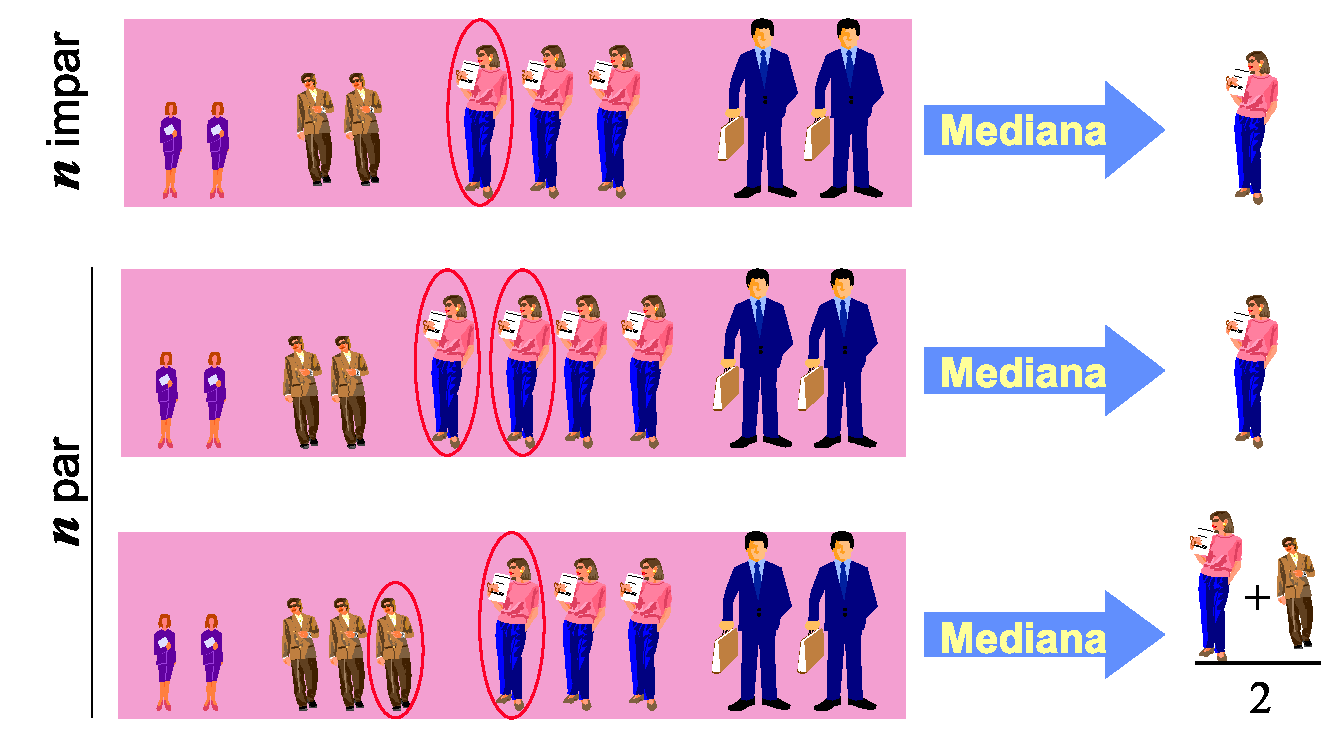
\includegraphics[scale=0.4]{img/descriptiva/mediana}
% \end{center}
% \note{Una vez ordenados los valores de la muestra de menor a mayor, el cálculo de la mediana con datos no agrupados,
% depende de si el tamaño de la muestra es par o impar. Si es impar, entonces habrá un único valor central que ocupará la posición $\frac{n+1}{2}$ y dicho valor será la mediana.
% Mientras que si el tamaño muestral es par, entonces habrá dos valores centrales, que ocuparan las posiciones
% $\frac{n}{2}$ y $\frac{n}{2}+1$. Si estos valores son iguales, la mediana será ese valor, mientras que si son
% distintos, la mediana estará entre los valores que ocupan estas posiciones y si puede se calculará su media aritmética.
% }
% \end{frame}
% 
% 
% %---------------------------------------------------------------------slide----
% \begin{frame}
% \frametitle{Cálculo de la mediana}
% \framesubtitle{Ejemplo con datos no agrupados}
% En el ejemplo anterior del número de hijos, el tamaño muestral es 25, de manera que al ser impar se deben ordenar los
% datos de menor a mayor y buscar el que ocupa la posición $\frac{25+1}{2} = 13$.
% \[
% 0,0,1,1,1,1,1,1,2,2,2,2,\fbox{2},2,2,2,2,2,2,2,2,2,3,3,4
% \]
% y la mediana es 2 hijos.
% 
% Si se trabaja con la tabla de frecuencias, se debe buscar el primer valor cuya frecuencia absoluta acumulada iguala o
% supera a 13, que es la posición que le corresponde a la mediana, o bien el primer valor cuya frecuencia relativa
% acumulada iguala o supera a $0.5$:
% \[
% \setlength\arraycolsep{3mm}
% \setlength\arrayrulewidth{0.5pt}
% \begin{array}{rrrrr}
% \hline
% x_i & n_i & f_i & N_i & F_i\\
% \hline
% 0 & 2 & 0.08 & 2 & 0.08\\
% 1 & 6 & 0.24 & 8 & 0.32\\
% \rowcolor{coral} \fbox{2} & 14 & 0.56 & 22 & 0.88\\
% 3 & 2  & 0.08 & 24 & 0.96\\
% 4 & 1 & 0.04 & 25 & 1 \\ 
% \hline 
% \sum & 25 & 1 \\
% \hline
% \end{array}
% \]
% 
% \note{Volviendo al ejemplo del número de hijos en una muestra de 25 matrimonios, para calcular la mediana, primero se
% ordenan los datos de menor a mayor, y después se busca el valor centra, que en este caso, al ser un tamaño impar, es
% único y ocupa la posición $\frac{25+1}{2}$ que vale 13. Contamos 1,2, hasta la 13 y observalos que el valor que aparece
% es un 2. Luego la mediana es 2 hijos.
% 
% Para calcular la mediana a partir de la tabla de frecuencias, hay que buscar de nuevo el individuo que ocupa la
% posición 13, y para ello se busca en la tabla el valor que tiene una frecuencia absoluta acumulada igual o mayor que 13.
% En la tabla se puede observar que la primera frecuencia absoluta acumulada que iguala o supera al 13 es 22 y
% corresponde al valor 2 que es la mediana.
% }
% \end{frame}
% 
% 
% %---------------------------------------------------------------------slide----
% \begin{frame}
% \frametitle{Cálculo de la mediana con datos agrupados}
% Con datos agrupados la mediana se calcula interpolando en el polígono de frecuencias absolutas acumuladas para el valor $n/2$.
% \begin{center}
% \scalebox{0.7}{\begin{pspicture}(0,-3.65375)(13,4)
\rput(1.9442188,-2.38625){\psaxes[linewidth=0.04,labels=none,ticksize=0.0958cm,dx=10.0cm,dy=6.0cm,Dx=10,Dy=5](0,0)(0,0)(10.01,6.01)}
\rput[c](7,-3.47625){$X$}
\rput{-270.0}(1.4,0.5359375){\rput(0.1621875,0.72375){Frecuencia Absoluta Acumulada $N_i$}}
\psline[linewidth=0.04,linecolor=blue](1.9642187,-2.38625)(3.9642189,-1.98625)(5.9642186,-0.38625)(7.9642186,1.81375)(9.964219,3.21375)(11.964219,3.61375)
\psline[linewidth=0.04,linecolor=orange,linestyle=dashed,dash=0.16cm 0.16cm](1.9642187,0.61375)(6.9,0.61375)(6.9,-2.38625)
\rput[r](1.6,0.62){$\dfrac{n}{2}$}
\rput[r](1.6,3.6){$n$}
\rput[c](7,-2.8){Mediana}
\end{pspicture}}
% \end{center}
% \note{Cuando se trabaja con datos agrupados en clases, la mediana se calcula de forma aproximada, interpolando en el
% polígono de frecuencias acumuladas para el valor $n/2$. 
% 
% La interpolación consiste en proyectar sobre el polígono la frecuencia $n/2$ y ver a qué altura del eje de abscisas
% corta al polígono de frecuencias. Dicho valor es la mediana.
% }
% \end{frame}
% 
% 
% %---------------------------------------------------------------------slide----
% \begin{frame}
% \frametitle{Interpolación en el polígono de frecuencias absolutas acumuladas}
% \begin{center}
% \scalebox{1}{\begin{pspicture}(-1,-0.5)(9,5)
\psaxes[arrows=->,ticks=none,labels=none](0,0)(0,0)(6,5)
\pspolygon[fillcolor=royalblue1,fillstyle=solid,linestyle=none](1,1)(5,4)(5,1)
\uncover<2-3>{\pspolygon[fillcolor=coral,fillstyle=solid,linestyle=none](1,1)(3.67,3)(3.67,1)}
\psline[linestyle=dashed](0,1)(5,1)
\psline[linestyle=dashed](0,4)(5,4)
\psline[linestyle=dashed](1,0)(1,1)
\psline[linestyle=dashed](5,0)(5,4)
\psline[linecolor=blue](1,1)(5,4)
\psarc(1,1){0.3}{0}{35}
\rput[r](-0.1,1){$N_{i-1}$}
\rput[r](-0.1,4){$N_{i}$}
\rput[t](1,-0.1){$l_{i-1}$}
\rput[t](5,-0.1){$l_{i}$}
\rput[l](1.4,1.2){$\alpha$}
\rput[l](6,3){\color{royalblue1} $\tg(\alpha) = \dfrac{N_i-N_{i-1}}{l_i-l_{i-1}}$}
\uncover<2->{
\rput[r](-0.1,3){$n/2$}
\psline[linestyle=dashed](0,3)(3.67,3)
\psline[linestyle=dashed](3.67,0)(3.67,3)
\rput[t](3.67,-0.1){$Me$}
%\pspolygon[fillcolor=coral,fillstyle=solid,linestyle=none](1,1)(3.67,3)(3.67,1)
\rput[l](6,2){\color{coral}$\tg(\alpha) = \dfrac{n/2-N_{i-1}}{Me-l_{i-1}}$}
}
\end{pspicture}}
% \end{center}
% 
% \uncover<3->{
% \[
% Me = l_{i-1}+\frac{n/2 - N_{i-1}}{N_i-N_{i-1}}(l_i-l_{i-1}) = l_{i-1}+\frac{n/2-N_{i-1}}{n_i}a_i
% \]
% }
% 
% \note{La interpolación en realidad consiste en una razón de semejanza de triángulos. 
% 
% En primer lugar se identifica el intervalo en el que cae la mediana, mirando en la columna de frecuencias acumuladas de
% la tabla de frecuencias, de igual modo a como se hace para datos no agrupados. Una vez identificado el intervalo, se
% toma el segmento del polígono de frecuencias acumuladas que corresponde a dicho intervalo. Supongamos que dicho
% intervalo tiene límite inferior $l_{i-1}$ y límite superior $l_i$, y que parte de una frecuencia absoluta acumulada
% $N_{i-1}$ y llega a una frecuencia absoluta acumulada $N_{i}$. Este segmento define un triángulo rectángulo de ángulo
% $\alpha$ cuya tangente es el cateto opuesto, que vale $N_i-N_{i-1}$ entre el cateto contiguo, que es precisamente la
% amplitud del intervalo $l_i-l_{i-1}$.
% 
% Por otro lado, si proyectamos la frecuencia corresondiente a la media $n/2$ sobre el polígono, en el punto de corte
% aparecería la mediana, de manera se se tiene otro triángulo rectángulo más pequeño que es semejante al anterior al
% compartir el mismo ángulo $\alpha$. Al igual que antes, la tangente de este ángulo será el cateto opuesto, que ahora
% vale $n/2-N_i$ entre el cateto contiguo que ahora vale $Me-l_{i-1}$. 
% 
% Puesto que se trata del mismo ángulo, su tangente es la misma y se pueden igual ambas expresiones, dando lugar a una
% ecuación conde la única incógnita es la mediana. Despejandola, se obtiene la fórmula para calcular la mediana.
% }
% \end{frame}
% 
% 
% %---------------------------------------------------------------------slide----
% \begin{frame}
% \frametitle{Cálculo de la mediana}
% \framesubtitle{Ejemplo con datos agrupados}
% En el ejemplo de las estaturas $n/2 =
% 30/2 = 15$. Si miramos en el polígono de frecuencias acumuladas comprobamos que
% la mediana caerá en el intervalo $(170,180]$.
% \begin{center}
% \scalebox{0.7}{% Created by tikzDevice version 0.8.1 on 2015-11-09 19:55:17
% !TEX encoding = UTF-8 Unicode
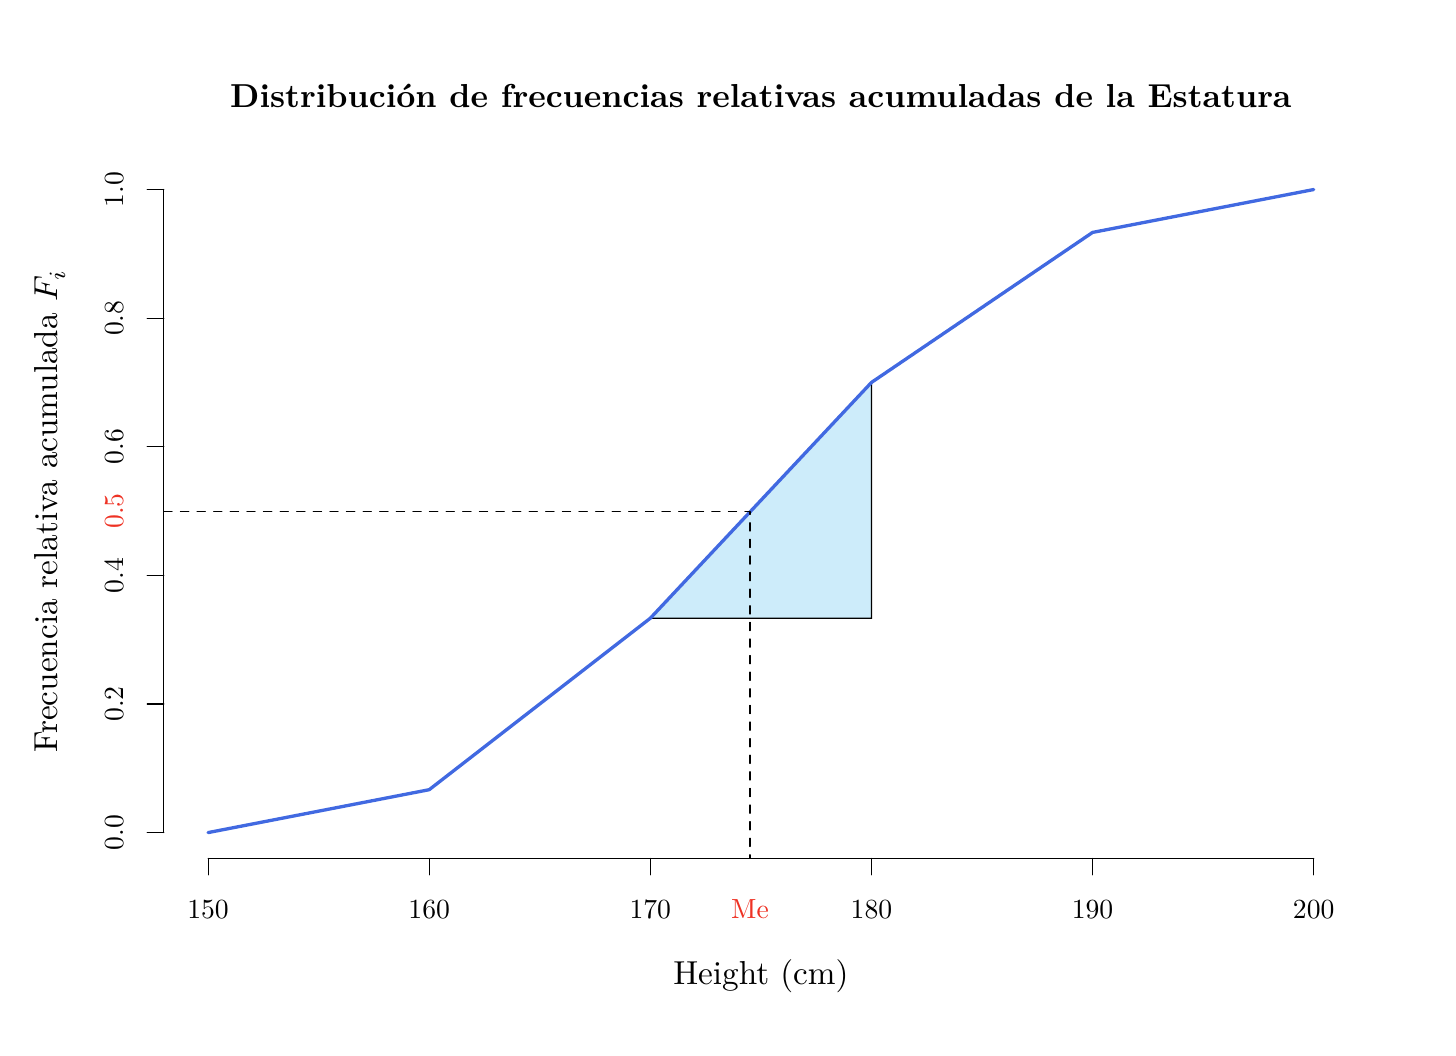
\begin{tikzpicture}[x=1pt,y=1pt]
\definecolor{fillColor}{RGB}{255,255,255}
\path[use as bounding box,fill=fillColor,fill opacity=0.00] (0,0) rectangle (505.89,361.35);

\path[clip] (  0.00,  0.00) rectangle (505.89,361.35);
\definecolor{drawColor}{RGB}{0,0,0}

\node[text=drawColor,anchor=base,inner sep=0pt, outer sep=0pt, scale=  1.20] at (264.95,332.61) {\bfseries Distribución de frecuencias relativas acumuladas de la Estatura};

\node[text=drawColor,anchor=base,inner sep=0pt, outer sep=0pt, scale=  1.20] at (264.95, 15.60) {Height (cm)};

\node[text=drawColor,rotate= 90.00,anchor=base,inner sep=0pt, outer sep=0pt, scale=  1.20] at ( 10.80,186.67) {Frecuencia relativa acumulada $F_i$};

\path[clip] (  0.00,  0.00) rectangle (505.89,361.35);
\definecolor{drawColor}{RGB}{0,0,0}

\onslide<3->{\draw[fill=color1!20] (224.99,147.95) -- (304.90,233.15) -- (304.90,147.95) -- cycle;}

\path[draw=drawColor,line width= 0.4pt,line join=round,line cap=round] ( 65.18, 61.20) -- (464.71, 61.20);

\path[draw=drawColor,line width= 0.4pt,line join=round,line cap=round] ( 65.18, 61.20) -- ( 65.18, 55.20);

\path[draw=drawColor,line width= 0.4pt,line join=round,line cap=round] (145.09, 61.20) -- (145.09, 55.20);

\path[draw=drawColor,line width= 0.4pt,line join=round,line cap=round] (224.99, 61.20) -- (224.99, 55.20);

\path[draw=drawColor,line width= 0.4pt,line join=round,line cap=round] (304.90, 61.20) -- (304.90, 55.20);

\path[draw=drawColor,line width= 0.4pt,line join=round,line cap=round] (384.80, 61.20) -- (384.80, 55.20);

\path[draw=drawColor,line width= 0.4pt,line join=round,line cap=round] (464.71, 61.20) -- (464.71, 55.20);

\node[text=drawColor,anchor=base,inner sep=0pt, outer sep=0pt, scale=  1.00] at ( 65.18, 39.60) {150};

\node[text=drawColor,anchor=base,inner sep=0pt, outer sep=0pt, scale=  1.00] at (145.09, 39.60) {160};

\node[text=drawColor,anchor=base,inner sep=0pt, outer sep=0pt, scale=  1.00] at (224.99, 39.60) {170};

\node<2->[text=color2,anchor=base,inner sep=0pt, outer sep=0pt, scale=1.00] at (261, 39.60) {Me};

\node[text=drawColor,anchor=base,inner sep=0pt, outer sep=0pt, scale=  1.00] at (304.90, 39.60) {180};

\node[text=drawColor,anchor=base,inner sep=0pt, outer sep=0pt, scale=  1.00] at (384.80, 39.60) {190};

\node[text=drawColor,anchor=base,inner sep=0pt, outer sep=0pt, scale=  1.00] at (464.71, 39.60) {200};

\path[draw=drawColor,line width= 0.4pt,line join=round,line cap=round] ( 49.20, 70.49) -- ( 49.20,302.86);

\path[draw=drawColor,line width= 0.4pt,line join=round,line cap=round] ( 49.20, 70.49) -- ( 43.20, 70.49);

\path[draw=drawColor,line width= 0.4pt,line join=round,line cap=round] ( 49.20,116.97) -- ( 43.20,116.97);

\path[draw=drawColor,line width= 0.4pt,line join=round,line cap=round] ( 49.20,163.44) -- ( 43.20,163.44);

\path[draw=drawColor,line width= 0.4pt,line join=round,line cap=round] ( 49.20,209.91) -- ( 43.20,209.91);

\path[draw=drawColor,line width= 0.4pt,line join=round,line cap=round] ( 49.20,256.38) -- ( 43.20,256.38);

\path[draw=drawColor,line width= 0.4pt,line join=round,line cap=round] ( 49.20,302.86) -- ( 43.20,302.86);

\node[text=drawColor,rotate= 90.00,anchor=base,inner sep=0pt, outer sep=0pt, scale=  1.00] at ( 34.80, 70.49) {0.0};

\node[text=drawColor,rotate= 90.00,anchor=base,inner sep=0pt, outer sep=0pt, scale=  1.00] at ( 34.80,116.97) {0.2};

\node[text=drawColor,rotate= 90.00,anchor=base,inner sep=0pt, outer sep=0pt, scale=  1.00] at ( 34.80,163.44) {0.4};

\node<2->[text=color2,rotate= 90.00,anchor=base,inner sep=0pt, outer sep=0pt, scale=  1.00] at ( 34.80,186.675)
{0.5};

\node[text=drawColor,rotate= 90.00,anchor=base,inner sep=0pt, outer sep=0pt, scale=  1.00] at ( 34.80,209.91) {0.6};

\node[text=drawColor,rotate= 90.00,anchor=base,inner sep=0pt, outer sep=0pt, scale=  1.00] at ( 34.80,256.38) {0.8};

\node[text=drawColor,rotate= 90.00,anchor=base,inner sep=0pt, outer sep=0pt, scale=  1.00] at ( 34.80,302.86) {1.0};

\path[clip] ( 49.20, 61.20) rectangle (480.69,312.15);

\definecolor{fillColor}{RGB}{137,211,243};

\definecolor{drawColor}{RGB}{65,105,225};

\path[draw=drawColor,line width= 1.2pt,line join=round,line cap=round] ( 65.18, 70.49) --
	(145.09, 85.99) --
	(224.99,147.95) --
	(304.90,233.15) --
	(384.80,287.36) --
	(464.71,302.86);

\onslide<2->{
\definecolor{drawColor}{RGB}{0,0,0}
\path[draw=drawColor,line width= 0.4pt,line join=round,line cap=round] ( 49.20,186.675) -- ( 43.20,186.675);
\path[draw=drawColor,line width= 0.4pt,line join=round,line cap=round, dashed] ( 49.20,186.675) -- ( 261,186.675) --
(261,61.20);
\path[draw=drawColor,line width= 0.4pt,line join=round,line cap=round] (261, 61.20) -- (261, 55.20);
}

\end{tikzpicture}
}
% \end{center}
% \note{Veamos un ejemplo de interpolación para calcular la mediana de la muestra de estaturas. Mirando en la tabla de
% frecuencias se observa que el primer intervalo con una frecuencia igual o mayor que $n/2=30/2=15$ es el que va de 170
% cm a 180 cm, así que se toma el trozo del polígono de frecuencias absolutas acumuladas corresondiente a este intervalo.
% }
% \end{frame}
% 
% 
% %---------------------------------------------------------------------slide----
% \begin{frame}
% \frametitle{Interpolación en el polígono de frecuencias absolutas acumuladas}
% \begin{center}
% \scalebox{1}{% Author: Alfredo Sánchez Alberca (asalber@ceu.es)

\pgfplotsset{
    standard/.style={
        axis x line=middle,
        axis y line=middle,
        % enlarge x limits=0.15,
        % enlarge y limits=0.15,
        every axis x label/.style={at={(current axis.right of origin)},anchor=north west},
        every axis y label/.style={at={(current axis.above origin)},anchor=north east}
    }
}

\begin{tikzpicture}
\begin{axis}[standard,xlabel={$X$}, ylabel={$F$}, axis equal, xmin=-0.1, xmax=7, ymin=0,
ymax=5, xtick={1,6}, xticklabels={$170$,$180$}, ytick={1,4}, yticklabels={$0.34$,$0.70$}]

\coordinate (A) at (axis cs:6,1);
\coordinate (B) at (axis cs:1,1);
\coordinate (C) at (axis cs:6,4);
\coordinate (D) at (axis cs:4,1);
\coordinate (E) at (axis cs:4,2.8);
\coordinate (F) at (axis cs:-0.1,2.8);
\coordinate (G) at (axis cs:4,-0.1);
\end{axis}

\draw (B) -- (C);

\pause

\draw[fill=color1!20] (A) -- (B) -- (C) -- cycle;
\draw<4->[fill=color2!20] (D) -- (B) -- (E) -- cycle;

\tkzMarkAngle[fill= green!50,size=1cm](A,B,C);
\tkzLabelAngle[pos = 0.7](A,B,C){$\alpha$};
\node[anchor=west] at (7,3) {$\color{color1} \displaystyle \operatorname{tg}(\alpha) = \frac{0.7-0.34}{180-170}$};

\pause

\node[anchor=east] at (F) {$0.5$};
\draw[dashed] (F) -- (E) -- (G);
\node[anchor=north] at (G) {\color{color2}$Me$};

\pause 

\node[anchor=west] at (7,2) {$\color{color2} \displaystyle \operatorname{tg}(\alpha) = \frac{0.5-0.34}{Me-170}$};


\end{tikzpicture}}
% \end{center}
% 
% \uncover<3->{
% \[
% Med = 170+\frac{15 - 10}{21-10}(180-170) = 170+\frac{5}{11}10 = 174.54
% \]
% }
% 
% \note{Si nos fijamos en el triángulo grande, la tangente de $\alpha$ vale $21-10$ que es el cateto opuesto, entre
% $180-170$ que es el cateto contiguo, mientras que si nos fijamos en el triángulo pequeño que aparece al proyectar $15$
% sobre el polígono, se tiene que la tangente de $\alpha$ vale $15-10$ que es cateto opuesto entre $Me-170$ que es el
% cateto contiguo. Igualando ambas expresiones y despejando la mediana se obtiene $174.54$ cm que es la estatura mediana.
% 
% Una comprobación que conviene hacer siempre es ver que el valor obtenido cae efectivamente dentro del intervalo de
% interpolación.}
% \end{frame}
% 
% 
% %---------------------------------------------------------------------slide----
% \begin{frame}
% \frametitle{Moda}
% \begin{definicion}[Moda muestral $Mo$]
% La \emph{moda muestral} de una variable $X$ es el valor de la variable más frecuente en la muestra.
% \end{definicion}
% Con datos agrupados se toma como clase modal la clase con mayor frecuencia en la muestra.
% 
% En ocasiones puede haber más de una moda.
% \begin{center}
% 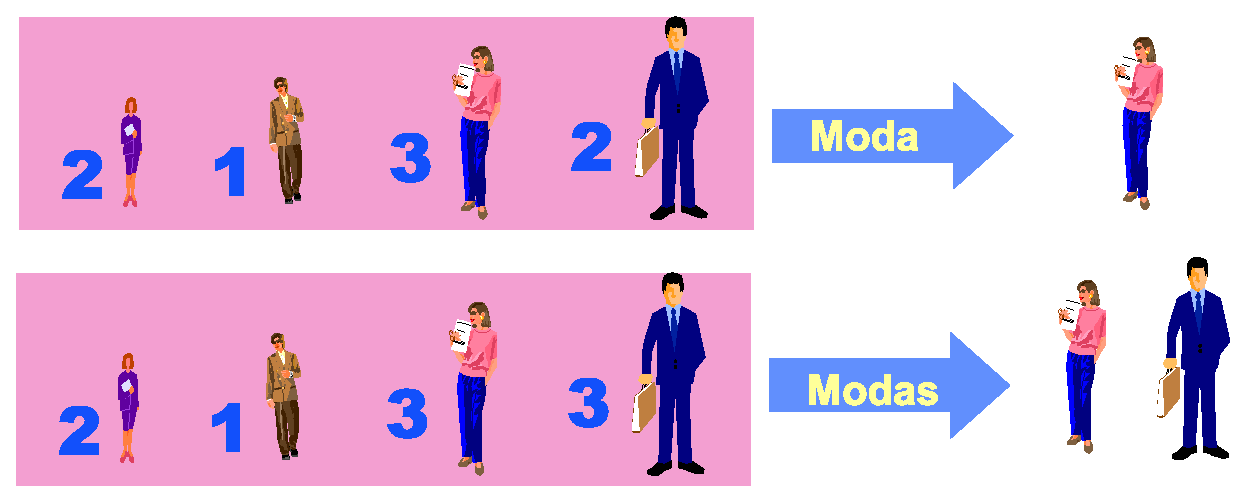
\includegraphics[scale=0.5]{img/descriptiva/moda}
% \end{center}
% \note{El último estadístico de tendencia central que veremos se llama moda, y viene a suplir las carencias de la media
% y mediana, que no podían calcularse para atributos nominales.
% 
% La moda se define como el valor más frecuente en la muestra, y puede ocurrir que en algunas distribuciones haya más de
% una moda.
% }
% \end{frame}
% 
% 
% %---------------------------------------------------------------------slide----
% \begin{frame}
% \frametitle{Cálculo de la moda}
% En el ejemplo del número de hijos puede verse fácilmente en la tabla de frecuencias que la moda es $Mo = 2$ hijos. 
% \begin{center}
% \setlength\arraycolsep{3mm}
% \setlength\arrayrulewidth{0.5pt}
% \begin{array}{rr}
% \hline
% \multicolumn{1}{c}{x_i} & \multicolumn{1}{c}{n_i} \\
% \hline
% 0 & 2 \\
% 1 & 6 \\
% \rowcolor{coral} \fbox{2} & 14 \\
% 3 & 2  \\
% 4 & 1 \\ 
% \hline 
% \end{array}
% \end{center}
% Y en el ejemplo de las estaturas también puede verse en la tabla de frecuencias que la clase modal es $Mo=(170,180]$.
% \begin{center}
% \setlength\arraycolsep{3mm}
% \setlength\arrayrulewidth{0.5pt}
% \begin{array}{rr}
% \hline
% \multicolumn{1}{c}{x_i} & \multicolumn{1}{c}{n_i} \\
% \hline
% (150,160] & 2 \\
% (160,170] & 8 \\
% \rowcolor{coral} \fbox{(170,180]} & 11 \\
% (180,190] & 7 \\
% (190,200] & 2 \\ 
% \hline 
% \end{array}
% \end{center}
% \note{La moda es el estadístico más sencillo de calcular pues sólo hay que fijarse en la columna de frecuencias
% absolutas de la tabla de frecuencias, buscar la mayor y ver a qué valor le corresponde.
% 
% En el ejemplo del número de hijos, la mayor frecuencia es 14, que le corresponde al 2, de manera que la moda es 2 hijos.
% 
% En el ejemplo de las estaturas, la mayor frecuencia es 11, que le corresponde al intervalo $(170,180]$ que es el
% intervalo modal.}
% \end{frame}
% 
% 
% %---------------------------------------------------------------------slide----
% \begin{frame}
% \frametitle{¿Qué estadístico de tendencia central usar?}
% En general, siempre que puedan calcularse conviene tomarlas en el siguiente orden:
% \begin{enumerate}
% \item Media. La media utiliza más información que el resto ya que para calcularla se tiene en cuenta la magnitud de los datos.
% \item Mediana. La mediana utiliza menos información que la media, pero más que la moda, ya que para calcularla se tiene
% en cuenta el orden de los datos.
% \item Moda. La moda es la que menos información utiliza ya que para calcularla sólo se tienen en cuenta las frecuencias absolutas.
% \end{enumerate}
% Pero, ¡ojo! la media también es muy sensible a los datos atípicos, así que, tampoco debemos perder de vista la mediana.
% 
% Por ejemplo, consideremos la siguiente muestra del número de hijos de 7 matrimonios:
% \begin{center}
% 0, 0, 1, 1, 2, 2, 15
% 
% $\bar{x}=3$ hijos \quad y \quad $Me=1$ hijos
% 
% \emph{¿Qué representante de la muestra tomarías?}
% \end{center}
% 
% \note{Hemos visto tres estadístico de tendencia central, de manera que surge la pregunta de cuál usar en el caso de que
% puedan calcularse los tres. 
% 
% En principio, siempre que pueda calcularse se tomará la media, pues es la medida que más información utiliza de la
% muestra al tener en cuenta la magnitud de los datos. Si no puede calcularse la media, se utilizará la mediana, que
% aunque no tiene en cuenta la magnitud de los valores, al menos si tiene en cuenta el orden entre ellos. Y finalmente,
% si no se pueden calcular ninguna de las dos, se tomará la moda que únicamente tiene en cuenta las frecuencias de los
% valores.
% 
% Una excepción a esta regla es cuando en la muestra haya datos atípicos, ya que la media es muy sensible a datos
% atípicos, mientras que la mediana no lo es apenas. Si nos fijamos en esta pequeña muestra con el número de hijos de 7
% matrimonios, con un matrimonio que es claramente atípico por tener 15 hijos, podemos ver que la media vale 3 hijos,
% mientras que sin el dato atípico valdría 1 hijo. Es decir, la media se ve muy alterada por el dato atípico. Si embargo
% la mediana vale 1 hijo tanto con el dato atípico como sin el. En estas circunstancias es mejor utilizar la mediana como
% medida de representatividad.}
% \end{frame}
% 
% 
% %---------------------------------------------------------------------slide----
% \begin{frame}
% \frametitle{Cuantiles}
% Son valores de la variable que dividen la distribución, supuesta ordenada de menor a mayor, en partes que contienen el mismo número de datos.
% 
% Los más utilizados son:
% \begin{description}
% \item[Cuartiles:] Dividen la distribución en 4 partes iguales.\\
% Hay tres cuartiles: $C_1$ (25\% acumulado) , $C_2$ (50\% acumulado), $C_3$ (75\% acumulado). 
% \item[Deciles:] Dividen la distribución en 10 partes iguales.\\
% Hay 9 deciles: $D_1$ (10\% acumulado) ,\ldots, $D_9$ (90\% acumulado).
% \item[Percentiles:] Dividen la distribución en 100 partes iguales.\\
% Hay 99 percentiles: $P_1$ (1\% acumulado),\ldots, $P_{99}$ (99\% acumulado).
% \end{description}
% 
% \note{Una vez vistas las medidas de tendencia central, pasamos al resto de medidas de posición que son los cuantiles y
% que dividen la muestra en partes iguales. Existen distintos tipos:
% \begin{description}
% \item[Cuartiles:] Dividen la distribución en 4 partes iguales.\\
% Hay tres cuartiles: $C_1$ (25\% acumulado) , $C_2$ (50\% acumulado), $C_3$ (75\% acumulado). \\
% Obsérvese que la mediana coincide con el segundo cuartil.
% \item[Deciles:] Dividen la distribución en 10 partes iguales.\\
% Hay 9 deciles: $D_1$ (10\% acumulado) ,\ldots, $D_9$ (90\% acumulado).
% \item[Percentiles:] Dividen la distribución en 100 partes iguales.\\
% Hay 99 percentiles: $P_1$ (1\% acumulado),\ldots, $P_{99}$ (99\% acumulado).
% \end{description}
% 
% Obsérvese la correspondencia que hay entre algunos cuantiles, como por ejemplo el primer cuartil que se corresponde con
% el pertencil 25 o el tercer cuartil que se corresponde con el percentil 75. 
% }
% \end{frame}
% 
% 
% %---------------------------------------------------------------------slide----
% \begin{frame}
% \frametitle{Cálculo de los cuantiles}
% Los cuantiles se calculan de forma similar a la mediana. Por ejemplo, en el caso de los cuartiles se buscan los valores que tienen frecuencias absolutas acumuladas $n/4$ (primer cuartil), $n/2$ (segundo cuartil) y $3n/4$ (tercer cuartil) y si se trata de datos agrupados se interpola sobre el polígono de frecuencias acumuladas.
% \begin{center}
% \begin{center}
% \scalebox{0.7}{
% \begin{pspicture}(0,-3.65375)(13,4)
% \rput(1.9442188,-2.38625){\psaxes[linewidth=0.04,labels=none,ticksize=0.0958cm,dx=10.0cm,dy=6.0cm,Dx=10,Dy=5](0,0)(0,0)(10.01,6.01)}
% \rput[c](7,-3.47625){$X$}
% \rput{-270.0}(1.4,0.5359375){\rput(0.1621875,0.72375){Frecuencia Absoluta Acumulada $N_i$}}
% \psline[linewidth=0.04,linecolor=blue](1.9642187,-2.38625)(3.9642189,-1.98625)(5.9642186,-0.38625)(7.9642186,1.81375)(9.964219,3.21375)(11.964219,3.61375)
% \psline[linewidth=0.04,linecolor=orange,linestyle=dashed,dash=0.16cm 0.16cm](1.9642187,0.61375)(6.9,0.61375)(6.9,-2.38625)
% \psline[linewidth=0.04,linecolor=orange,linestyle=dashed,dash=0.16cm 0.16cm](1.9642187,2.11375)(8.3,2.11375)(8.3,-2.38625)
% \psline[linewidth=0.04,linecolor=orange,linestyle=dashed,dash=0.16cm 0.16cm](1.9642187,-0.88625)(5.3,-0.88625)(5.3,-2.38625)
% \rput[r](1.6,2.12){$\dfrac{3n}{4}$}
% \rput[r](1.6,0.62){$\dfrac{n}{2}$}
% \rput[r](1.6,-0.88){$\dfrac{n}{4}$}
% \rput[r](1.6,3.6){$n$}
% \rput[c](5.3,-2.8){$C_1$}
% \rput[c](6.9,-2.8){$C_2$}
% \rput[c](8.3,-2.8){$C_3$}
% \end{pspicture}}
% \end{center}
% \end{center}
% \note{Los cuantiles se calculan, al igual que la mediana, interpolando sobre el polígono de frecuencias absolutas
% acumuladas. Por ejemplo, para los cuartiles, proyectando la frecuencia absloluta acumulada del primer cuartil, que es
% $n/4$, se obtiene el primer cuartil, proyectando $n/2$ se obtiene el segundo cuartil, y proyectando $3n/4$ se obtiene
% el primer cuartil, y lo mismo para los otros cuantiles.}
% \end{frame}
% 
% 
% %---------------------------------------------------------------------slide----
% \begin{frame}
% \frametitle{Cálculo de los cuantiles}
% \framesubtitle{Ejemplo con datos no agrupados}
% En el ejemplo anterior del número de hijos se tenían la siguientes frecuencias relativas acumuladas
% \begin{center}
% \setlength\arraycolsep{3mm}
% \setlength\arrayrulewidth{0.5pt}
% \begin{array}{rr}
% \hline
% \multicolumn{1}{c}{x_i} & \multicolumn{1}{c}{F_i} \\
% \hline
% 0 & 0.08\\
% 1 & 0.32\\
% 2 & 0.88\\
% 3 & 0.96\\
% 4 & 1\\ 
% \hline
% \end{array}
% \end{center}
% \begin{align*}
% F_{C_1}=0.25 &\Rightarrow C_1 = 1 \text{ hijos},\\
% F_{C_2}=0.5 &\Rightarrow C_2 = 2 \text{ hijos},\\
% F_{C_3}=0.75 &\Rightarrow C_3 = 2 \text{ hijos},\\
% F_{D_3}=0.3 &\Rightarrow D_3 = 1 \text{ hijos},\\
% F_{P_{92}}=0.92 &\Rightarrow P_{92} = 3 \text{ hijos}.\\
% \end{align*}
% \note{Los cuantiles se calculan de forma similara a la mediana a partir de las frecuencias acumuladas correspondientes a cada uno de ellos.
% 
% En el ejemplo del número de hijos donde se tenían las frecuencias relativas acumuladas que aparecen en esta tabla, para calcular el primer
% cuartil se parte de su frecuencia relativa acumulada que es $0.25$ ya que hasta el primer cuartil se tienen acumulados el 25\% de los
% individuos y se busca en la tabla el primer valor cuya frecuencia relativa acumulada es igual o superior a $0.25$, que en este caso es 1
% hijo, ya que su frecuencia relativa acumulada es $0.32$ que supera a $0.25$ mientras que la frecuencia relativa acumulada del 0 no llega a
% $0.25$. Del mismo modo, el cuartil segundo, cuya frecuencia relativa acumulada es $0.5$, es 2 hijos y el tercer cuartil, con frecuencia
% relativa acumulada $0.75$ también es 2 hijos.
% 
% Para el decil tercero, su frecuencia relativa acumulada es $0.3$, y procediendo como para los cuartiles, se observa que el primer valor con
% frecuencia relativa acumulada igual o superior a $0.3$ es 1 hijo.
% 
% Finalmente, para el percentil 92, su frecuencia relativa acumulada es $0.92$ y el primer valor con frecuencia relativa acumulada igual o
% superior a este valor es 3 hijos.}
% \end{frame}
% 
% 
% \subsection{Estadísticos de dispersión}
% %---------------------------------------------------------------------slide----
% \begin{frame}
% \frametitle{Estadísticos de dispersión}
% Recogen información respecto a la heterogeneidad de la variable y a la concentración de sus valores en torno a algún valor central.
% 
% 
% Para las variables cuantitativas, las más empleadas son:
% \begin{itemize}
% \item Recorrido.
% \item Rango Intercuartílico.
% \item Varianza.
% \item Desviación Típica.
% \item Coeficiente de Variación.
% \end{itemize}
% \note{Uno de los aspectos más importantes de una muestra es la variabilidad de los datos, que también se conoce como
% dispersión de la muestra. Veremos hasta 5 estadísticos para describir la dispersión:
% \begin{itemize}
% \item Recorrido.
% \item Rango Intercuartílico.
% \item Varianza.
% \item Desviación Típica.
% \item Coeficiente de Variación.
% \end{itemize}
% }
% \end{frame}
% 
% 
% %---------------------------------------------------------------------slide----
% \begin{frame}
% \frametitle{Recorrido}
% \begin{definicion}[Recorrido muestral $Re$]
% El \emph{recorrido muestral} de una variable $X$ se define como la diferencia entre el máximo y el mínimo de los valores en la muestra.
% \[Re = \max_{x_i} -\min_{x_i}\]
% \end{definicion}
% El recorrido da una idea de la máxima variación que hay entre los datos muestrales. No obstante, es muy sensible a datos atípicos ya que suelen aparecer justo en los extremos de la distribución, por lo que no se suele utilizar mucho.
% 
% \begin{center}
% \scalebox{1} % Change this value to rescale the drawing.
% {
% \begin{pspicture}(-1,-1)(9,1)
% \psline[linewidth=0.04cm]{|-|}(0,0)(8,0)
% \rput[t](0,-0.2){$\min$}
% \rput[t](8,-0.2){$\max$}
% \psline[linecolor=orange]{<->}(0,0.5)(8,0.5)
% \rput[b](4,0.7){$Re$}
% \end{pspicture}}
% \end{center}
% \note{El recorrido es el estadístico de dispersión más natural ya que consiste en medir la distancia que va del mayor
% al menor de los valores y se calcula restándolos. 
% 
% Cuanto mayor sea el recorrido, mayor dispersión habrá en la muestra.
% 
% El principal problema que presenta el recorrido es que es muy sensible a los datos atípicos, ya que estos precisamente
% aparecen en los extremos de la distribución. }
% \end{frame}
% 
% 
% %---------------------------------------------------------------------slide----
% \begin{frame}
% \frametitle{Rango intercuartílico}
% Para evitar el problema de los datos atípicos en el recorrido, se puede utilizar el primer y tercer cuartil en lugar del mínimo y el máximo.
% \begin{definicion}[Rango intercuartílico muestral $RI$]
% El \emph{rango intercuartílico muestral} de una variable $X$ se define como la diferencia entre el tercer y el primer
% cuartil de la muestra. \[RI = C_3 -C_1\]
% \end{definicion}
% El rango intercuartílico da una idea de la variación que hay en el 50\% de los datos centrales. 
% 
% \begin{center}
% \scalebox{1} % Change this value to rescale the drawing.
% {
% \begin{pspicture}(-1,-1)(9,1)
% \psline[linewidth=0.04cm]{|-|}(0,0)(8,0)
% \rput[t](0,-0.2){$\min$}
% \rput[t](8,-0.2){$\max$}
% \psline[linewidth=0.04cm]{|-|}(2,0)(4,0)
% \psline[linewidth=0.04cm]{|-|}(0,0)(6,0)
% \rput[t](2,-0.2){$C_1$}
% \rput[t](4,-0.2){$C_2$}
% \rput[t](6,-0.2){$C_3$}
% \rput[b]](1,0.1){$25\%$}
% \rput[b]](3,0.1){$25\%$}
% \rput[b]](5,0.1){$25\%$}
% \rput[b]](7,0.1){$25\%$}
% \psline[linecolor=orange]{<->}(2,0.5)(6,0.5)
% \rput[b](4,0.7){$RI$}
% \end{pspicture}}
% \end{center}
% \note{Para evitar el problema que tiene el Recorrido con los datos atípicos, se suele utilizar el Rango
% Intercuartílico, que utiliza la misma idea del Recorrido pero midiendo la distancia que va del tercer al primer
% cuartil. 
% 
% Si recordamos, los cuartiles dividen la distribución en 4 partes iguales, de manera que entre el primer y el tercer
% cuartil estan el 50\% de los datos centrales de la distribución, y quedarían exlucidos el 25\% de valores menores y el
% 25\% de valores mayores, donde posiblemente estarían los datos atípicos. 
% 
% Por tanto el Rango Intercuartílico mide la dispersión central de la muestra, de manera que cuanto mayor sea, más
% dispersión central tendrá la muestra, aunque siempre hay que tener en cuenta las unidades de la variable al
% interpretarlo. }
% \end{frame}
% 
% 
% %---------------------------------------------------------------------slide----
% \begin{frame}
% \frametitle{Diagrama de caja y bigotes}
% La dispersión de una variable suele representarse gráficamente mediante un \highlight{\textbf{diagrama de caja y bigotes}}, que consiste en una caja sobre un eje $X$ donde el borde inferior de la caja es el primer cuartil, y el borde superior el tercer cuartil, y por tanto, la anchura de la caja es el rango intercuartílico.
% En ocasiones también se representa el segundo cuartil con una línea que divide la caja. 
% 
% También se utiliza para detectar los valores atípicos mediante unos segmentos (bigotes) que salen de los extremos de la caja y que marcan el intervalo de normalidad de los datos.
% \note{La dispersión de la muestra se representa a menudo mediante un diagrama de caja y bigotes, que como su propio
% nombre indica, consiste en una caja sobre un eje $X$ donde el borde inferior de la caja es el primer cuartil, y el
% borde superior el tercer cuartil, y por tanto, la anchura de la caja, por tanto, es el rango intercuartílico. 
% En ocasiones también se representa el segundo cuartil con una línea que divide la caja.
% 
% También se utiliza para detectar los valores atípicos de la muestra mediante unos segmentos llamados bigotes que
% salen de los extremos de la caja y que marcan el intervalo de normalidad de los datos.
% }
% \end{frame}
% 
% 
% %---------------------------------------------------------------------slide----
% \begin{frame}
% \frametitle{Diagrama de caja y bigotes}
% \framesubtitle{Ejemplo con pesos de recién nacidos}
% \begin{center}
% \scalebox{0.75}{% Created by tikzDevice version 0.8.1 on 2015-11-15 20:54:59
% !TEX encoding = UTF-8 Unicode
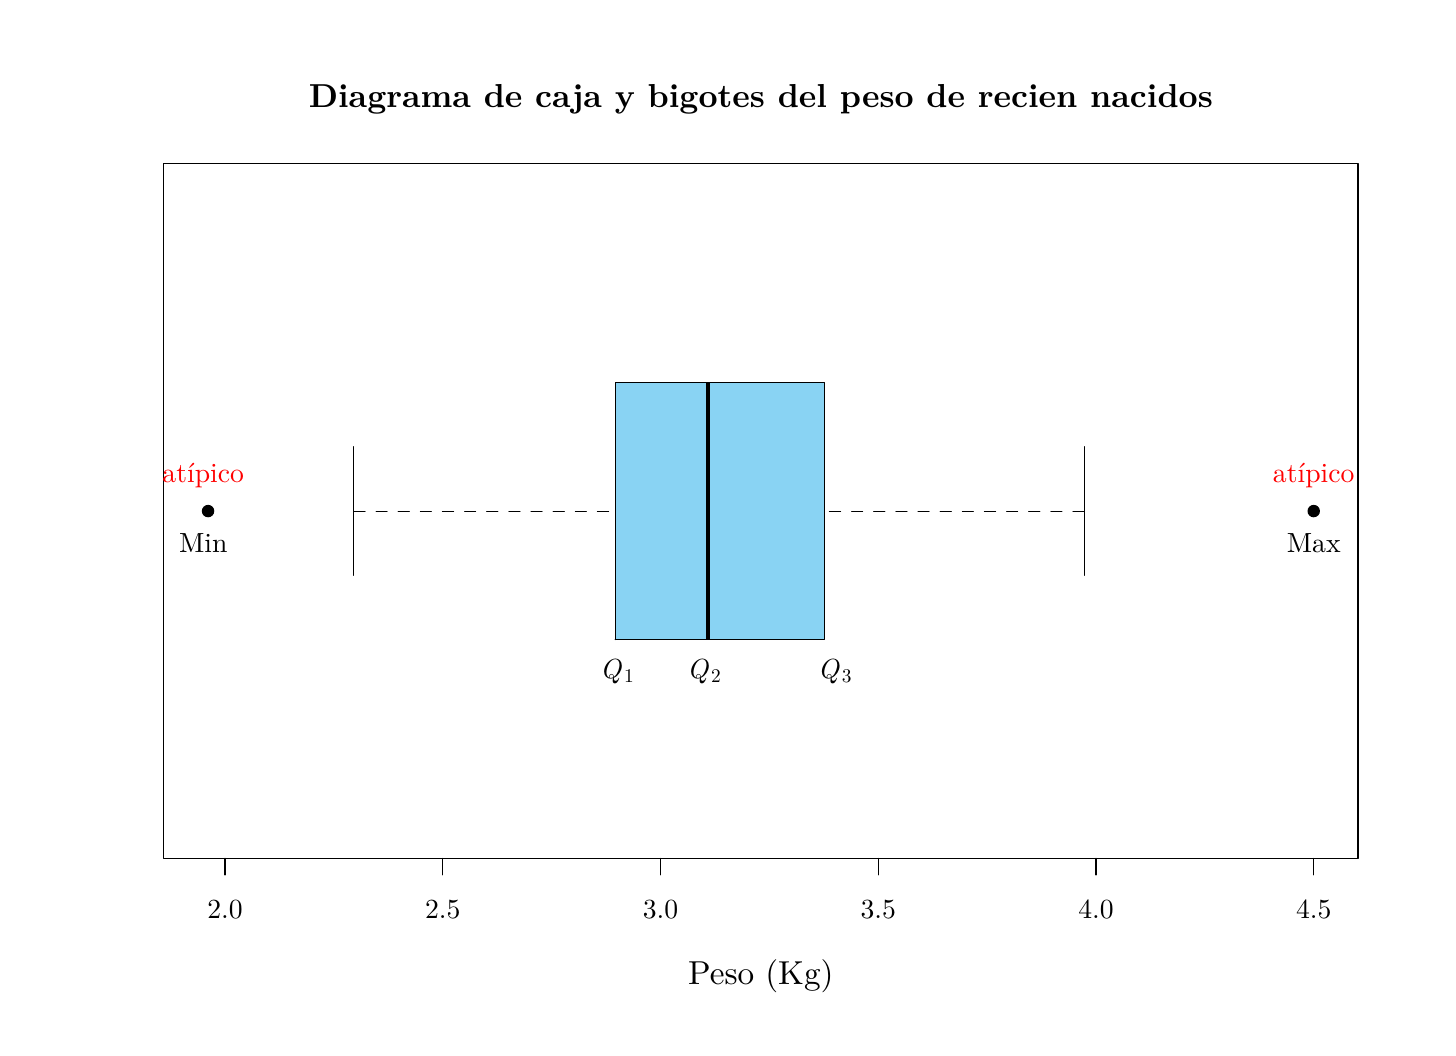
\begin{tikzpicture}[x=1pt,y=1pt]
\definecolor{fillColor}{RGB}{255,255,255}
\path[use as bounding box,fill=fillColor,fill opacity=0.00] (0,0) rectangle (505.89,361.35);
\begin{scope}
\path[clip] ( 49.20, 61.20) rectangle (480.69,312.15);
\definecolor{fillColor}{RGB}{137,211,243}

\path[fill=fillColor] (212.32,140.20) --
	(212.32,233.15) --
	(287.95,233.15) --
	(287.95,140.20) --
	cycle;
\definecolor{drawColor}{RGB}{0,0,0}

\path[draw=drawColor,line width= 1.2pt,line join=round] (245.85,140.20) -- (245.85,233.15);

\path[draw=drawColor,line width= 0.4pt,dash pattern=on 4pt off 4pt ,line join=round,line cap=round] (117.89,186.67) -- (212.32,186.67);

\path[draw=drawColor,line width= 0.4pt,dash pattern=on 4pt off 4pt ,line join=round,line cap=round] (381.73,186.67) -- (287.95,186.67);

\path[draw=drawColor,line width= 0.4pt,line join=round,line cap=round] (117.89,163.44) -- (117.89,209.91);

\path[draw=drawColor,line width= 0.4pt,line join=round,line cap=round] (381.73,163.44) -- (381.73,209.91);

\path[draw=drawColor,line width= 0.4pt,line join=round,line cap=round] (212.32,140.20) --
	(212.32,233.15) --
	(287.95,233.15) --
	(287.95,140.20) --
	(212.32,140.20);
\definecolor{fillColor}{RGB}{0,0,0}

\path[fill=fillColor] ( 65.18,186.67) circle (  2.25);

\path[fill=fillColor] (464.71,186.67) circle (  2.25);
\end{scope}
\begin{scope}
\path[clip] (  0.00,  0.00) rectangle (505.89,361.35);
\definecolor{drawColor}{RGB}{0,0,0}

\path[draw=drawColor,line width= 0.4pt,line join=round,line cap=round] ( 71.31, 61.20) -- (464.71, 61.20);

\path[draw=drawColor,line width= 0.4pt,line join=round,line cap=round] ( 71.31, 61.20) -- ( 71.31, 55.20);

\path[draw=drawColor,line width= 0.4pt,line join=round,line cap=round] (149.99, 61.20) -- (149.99, 55.20);

\path[draw=drawColor,line width= 0.4pt,line join=round,line cap=round] (228.67, 61.20) -- (228.67, 55.20);

\path[draw=drawColor,line width= 0.4pt,line join=round,line cap=round] (307.35, 61.20) -- (307.35, 55.20);

\path[draw=drawColor,line width= 0.4pt,line join=round,line cap=round] (386.03, 61.20) -- (386.03, 55.20);

\path[draw=drawColor,line width= 0.4pt,line join=round,line cap=round] (464.71, 61.20) -- (464.71, 55.20);

\node[text=drawColor,anchor=base,inner sep=0pt, outer sep=0pt, scale=  1.00] at ( 71.31, 39.60) {2.0};

\node[text=drawColor,anchor=base,inner sep=0pt, outer sep=0pt, scale=  1.00] at (149.99, 39.60) {2.5};

\node[text=drawColor,anchor=base,inner sep=0pt, outer sep=0pt, scale=  1.00] at (228.67, 39.60) {3.0};

\node[text=drawColor,anchor=base,inner sep=0pt, outer sep=0pt, scale=  1.00] at (307.35, 39.60) {3.5};

\node[text=drawColor,anchor=base,inner sep=0pt, outer sep=0pt, scale=  1.00] at (386.03, 39.60) {4.0};

\node[text=drawColor,anchor=base,inner sep=0pt, outer sep=0pt, scale=  1.00] at (464.71, 39.60) {4.5};
\end{scope}
\begin{scope}
\path[clip] (  0.00,  0.00) rectangle (505.89,361.35);
\definecolor{drawColor}{RGB}{0,0,0}

\node[text=drawColor,anchor=base,inner sep=0pt, outer sep=0pt, scale=  1.20] at (264.94,332.61) {\bfseries Diagrama de
caja y bigotes del peso de recien nacidos};

\node[text=drawColor,anchor=base,inner sep=0pt, outer sep=0pt, scale=  1.20] at (264.94, 15.60) {Peso (Kg)};
\end{scope}
\begin{scope}
\path[clip] (  0.00,  0.00) rectangle (505.89,361.35);
\definecolor{drawColor}{RGB}{0,0,0}

\path[draw=drawColor,line width= 0.4pt,line join=round,line cap=round] ( 49.20, 61.20) --
	(480.69, 61.20) --
	(480.69,312.15) --
	( 49.20,312.15) --
	( 49.20, 61.20);
\end{scope}
\begin{scope}
\path[clip] ( 49.20, 61.20) rectangle (480.69,312.15);
\definecolor{drawColor}{RGB}{0,0,0}

\node[text=drawColor,anchor=base west,inner sep=0pt, outer sep=0pt, scale=  1.00] at (206.83,126.11) {\itshape Q};

\node[text=drawColor,anchor=base west,inner sep=0pt, outer sep=0pt, scale=  0.70] at (215.53,124.61) {1};

\node[text=drawColor,anchor=base west,inner sep=0pt, outer sep=0pt, scale=  1.00] at (238.31,126.11) {\itshape Q};

\node[text=drawColor,anchor=base west,inner sep=0pt, outer sep=0pt, scale=  0.70] at (247.00,124.61) {2};

\node[text=drawColor,anchor=base west,inner sep=0pt, outer sep=0pt, scale=  1.00] at (285.51,126.11) {\itshape Q};

\node[text=drawColor,anchor=base west,inner sep=0pt, outer sep=0pt, scale=  0.70] at (294.21,124.61) {3};

\node[text=drawColor,anchor=base,inner sep=0pt, outer sep=0pt, scale=  1.00] at ( 63.44,171.61) {Min};

\node[text=drawColor,anchor=base,inner sep=0pt, outer sep=0pt, scale=  1.00] at (464.71,171.61) {Max};
\definecolor{drawColor}{RGB}{255,0,0}

\node[text=drawColor,anchor=base,inner sep=0pt, outer sep=0pt, scale=  1.00] at ( 63.44,197.17) {atípico};

\node[text=drawColor,anchor=base,inner sep=0pt, outer sep=0pt, scale=  1.00] at (464.71,197.17) {atípico};
\end{scope}
\end{tikzpicture}
}
% \end{center}
% \note{Aquí podemos ver un ejemplo de un diagrama de caja y bigotes para una muestra de pesos de recién nacidos. 
% El borde inferior de la caja corresponde al primer cuartil, que es aproximadamente $2.8$ Kg, el borde superior
% corresponde al tercer cuartil, que vale aproximadamente $3.4$ Kg, de manera que el ancho de la caja es el rango
% intercuartílico, y vale aproximadamente $0.6$ Kg, lo que indica una dispersión central baja, teniendo en cuenta que
% los pesos de los recién nacidos se suelen mover en unas unidades que van de 1 a 4 Kg, más o menos.
% 
% De la caja salen dos sementos, que son los bigotes, el inferior llega aproximadamente hasta $2.3$ Kg y el superior
% hasta $4$ Kg, delimitando el intervalo de normalidad de los datos, de manera que cualquier niño que pese menos de $2.3$
% Kg o más de $4$ Kg será un individuo atípico. De hecho en esta muestra aparecen dos pesos atípicos que aparecen
% marcados por puntos, uno que corresponde a un niño con 2 Kg de peso, y otro que corresponde a otro niño con 4.5 Kg de
% peso.}
% \end{frame}
% 
% 
% %---------------------------------------------------------------------slide----
% \begin{frame}
% \frametitle{Construcción del diagrama de caja y bigotes}
% \begin{enumerate}
% \item Calcular los cuartiles.
% \item Dibujar una caja de manera que el extremo inferior caiga sobre el primer cuartil y el extremo superior sobre el tercer cuartil.
% \item Dividir la caja con una línea que caiga sobre el segundo cuartil. 
% \item Para los bigotes inicialmente se determina la posición de los puntos denominados \emph{vallas} $v_1$ y $v_2$ restando y sumando respectivamente a primer y tercer cuartil $1.5$ veces el rango intercuartílico $RI$:
% \begin{align*}
% v_1&=C_1-1.5RI\\
% v_2&=C_3+1.5RI
% \end{align*}
% A partir de las vallas se buscan los valores $b_1$, que es el mínimo valor de la muestra mayor o igual que  $v_1$,
% y $b_2$, que es máximo valor de la muestra menor o igual que $v_2$. Para el bigote inferior se dibuja un segmento
% desde el borde inferior de la caja hasta $b_1$ y para el superior se dibuja un segmento desde el borde superior de la caja hasta $b_2$.
% \item Finalmente, si en la muestra hay algún dato por debajo de $v_1$ o por encima de $v_2$ se dibuja un punto sobre dicho valor. 
% \end{enumerate}
% \note{Para construcir el diagrama de cajas, hay que seguir los siguientes pasos:
% \begin{enumerate}
% \item Calcular los cuartiles.
% \item Dibujar una caja de manera que el extremo inferior caiga sobre el primer cuartil y el extremo superior sobre el tercer cuartil.
% \item Dividir la caja con una línea que caiga sobre el segundo cuartil. 
% \item Para los bigotes inicialmente se determina la posición de los puntos denominados \emph{vallas} $v_1$ y $v_2$ restando y sumando respectivamente a primer y tercer cuartil $1.5$ veces el rango intercuartílico $RI$:
% \begin{align*}
% v_1&=C_1-1.5RI\\
% v_2&=C_3+1.5RI
% \end{align*}
% A partir de las vallas se buscan los valores $b_1$, que es mínimo valor de la muestra mayor o igual que $v_1$,
% y $b_2$ es máximo valor de la muestra menor o igual que $v_2$. Para el bigote inferior se dibuja un segmento
% desde el borde inferior de la caja hasta $b_1$ y para el superior se dibuja un segmento desde el borde superior de la caja hasta $b_2$.
% \item Finalmente, si en la muestra hay algún dato por debajo de $v_1$ o por encima de $v_2$ se dibuja un punto sobre dicho valor. 
% \end{enumerate}}
% \end{frame}
% 
% 
% %---------------------------------------------------------------------slide----
% \begin{frame}
% \frametitle{Construcción del diagrama de caja y bigotes}
% \framesubtitle{Ejemplo del número de hijos}
% \begin{enumerate}
% \uncover<2->{\item Calcular los cuartiles: $C_1=1$ hijos} \uncover<3->{y $C_3=2$ hijos.}
% \uncover<4->{\item Dibujar la caja.}
% \uncover<5->{\item Calcular las vallas: $v_1=1-1.5*1=-0.5$ y $v_2=2+1.5*1=3.5$.}
% \uncover<6->{\item Dibujar los bigotes: $b_1=0$ hijos} \uncover<7->{y $b_1=3$ hijos.} 
% \uncover<8->{\item Dibujar los datos atípicos: 4 hijos.} 
% \end{enumerate}
% \begin{center}
% \scalebox{0.65}{%% Input file name: descriptiva/diagrama_caja_hijos.fig
%% FIG version: 3.2
%% Orientation: Landscape
%% Justification: Flush Left
%% Units: Inches
%% Paper size: A4
%% Magnification: 100.0
%% Resolution: 1200ppi

\begin{pspicture}(7.77cm,3.48cm)(16.66cm,12.45cm)
\psset{unit=0.8cm}
%%
%% Depth: 2147483647
%%
\newrgbcolor{mycolor0}{1.00 0.50 0.31}\definecolor{mycolor0}{rgb}{1.00,0.50,0.31}
%%
%% Depth: 100
%%
\psset{linestyle=solid,linecolor=black,fillstyle=none}
\psline(10.61,6.47)(19.94,6.47)
\psline(10.61,6.47)(10.61,6.26)
\psline(12.94,6.47)(12.94,6.26)
\psline(15.27,6.47)(15.27,6.26)
\psline(17.60,6.47)(17.60,6.26)
\psline(19.94,6.47)(19.94,6.26)
\rput(10.61,5.71){0}
\rput(12.94,5.71){1}
\rput(15.27,5.71){2}
\rput(17.60,5.71){3}
\rput(19.94,5.71){4}
\rput(15.27,15.49){Diagrama de caja y bigotes del número de hijos}
\rput(15.27,4.86){Número de hijos}
\psline(10.23,6.47)(20.31,6.47)(20.31,14.88)(10.23,14.88)(10.23,6.47)
\uncover<2->{
\psline(12.94,9.25)(12.94,12.51)
\rput(12.94,8.74){$C_1$}
}
\uncover<3->{
\psline(15.27,9.25)(15.27,12.51)
\rput(15.27,8.74){$C_3$}
}
\uncover<4->{
\psset{fillstyle=solid,fillcolor=mycolor0}
\pspolygon(12.94,9.25)(12.94,12.51)(15.27,12.51)(15.27,9.25)(12.94,9.25)
}
\uncover<6->{
\psline(10.61,10.06)(10.61,11.69)
\psset{linestyle=dashed}
\psline(10.61,10.88)(12.94,10.88)
}
\uncover<7->{
\psset{linestyle=solid}
\psline(17.60,10.06)(17.60,11.69)
\psset{linestyle=dashed}
\psline(17.60,10.88)(15.27,10.88)
}
\uncover<8->{
\psset{linestyle=solid,linecolor=black,fillstyle=solid,fillcolor=black}
\pscircle(19.94,10.88){0.1}
}
\end{pspicture}
%% End
}
% \end{center}
% \note{Veamos cómo construir el diagrama de caja y bigotes para el ejemplo del número de hijos:
% \begin{enumerate}
% \item Primero se calcula el primer cuartil que era 1 hijo y se dibuja el borde inferior de la caja. Después se calcula el tercer cuartil
% que era 3 hijos y se dibuja el borde superior de la caja.
% \item Una vez dibujados el borde inferior y superior de la caja se acaba de dibujar esta. 
% \item También se suele dibujar el cuartil segundo mediante una linea que divide la caja, pero en este ejemplo, al coincidir el cuartil
% segundo con el tercero, no se dibuja. 
% \item A continuación se calcula el rango intercuartílico que era 2-1=1 hijo y con el se calcula la valla inferior $v_1$ restandole al primer
% cuartil $1.5$ veces el rango intercuartílico, lo que nos da $-0.5$ hijos, y la valla superior $v_2$ sumandole al tercer cuartil $1.5$ veces
% el rango intercuartílico, lo que nos da $3.5$ hijos.
% \item Luego se calculan los extremos de los bigotes. El extremo del bigote inferior es $0$ hijos, ya que es el mínimo valor de la muestra
% por encima de la valla inferior que valía $-0.5$, y el bigote superiror es $3$ hijos, ya que es el máximo valor de la muestra por debajo de
% la valla superior que valía $3.5$ hijos. 
% \item Finalmente se dibujan los datos atípicos. Por debajo de la valla inferior no hay ningún valor en la muestra, pero por encima de la
% valla superior si hay una familia con 4 hijos, que se trata, por tanto, de una familia atípica y si se dibuja un punto en diagrama sobre
% dicho valor. 
% \end{enumerate}}
% \end{frame}
% 
% 
% %---------------------------------------------------------------------slide----
% \begin{frame}
% \frametitle{Desviaciones respecto de la media}
% Otra forma de medir la variabilidad de una variable es estudiar la concentración de los valores en torno a algún estadístico de tendencia central como por ejemplo la media. 
% 
% Para ello se suele medir la distancia de cada valor a la media. A ese valor se le llama
% \highlight{\textbf{desviación respecto de la media.}}
% \begin{center}
% \scalebox{1} % Change this value to rescale the drawing.
% {
% \begin{pspicture}(-1,-0.5)(7,1.5)
% \psline(0,0)(6,0)
% \psdots(1,0)(5,0)
% \psdot[linecolor=orange](3,0)
% \rput[t](3,-0.2){$\bar{x}$}
% \rput[t](1,-0.2){$x_i$}
% \rput[t](5,-0.2){$x_j$}
% \psline[linecolor=orange]{<->}(1,0.5)(3,0.5)
% \rput[b](2,0.7){$x_i-\bar{x}$}
% \rput[b](2,1.2){\scriptsize Desviación $-$}
% \psline[linecolor=orange]{<->}(3,0.5)(5,0.5)
% \rput[b](4,0.7){$x_j-\bar{x}$}
% \rput[b](4,1.2){\scriptsize Desviación $+$}
% \end{pspicture}}
% \end{center}
% 
% Si las desviaciones son grandes la media no será tan representativa como cuando la desviaciones sean pequeñas.
% \begin{center}
% \scalebox{1} % Change this value to rescale the drawing.
% {
% \begin{pspicture}(-1,-0.5)(7,1.6)
% \psline(0,1.6)(6,1.6)
% \psdots(0.1,1.6)(0.2,1.6)(0.4,1.6)(0.5,1.6)(0.8,1.6)(5,1.6)(5.3,1.6)(5.4,1.6)(5.7,1.6)(5.8,1.6)
% \psdot[linecolor=orange](3,1.6)
% \rput[t](3,1.4){$\bar{x}$}
% \rput[l](-2.5,1.6){\footnotesize Más dispersión}
% \rput[l](6.3,1.6){\footnotesize $\bar x$ menos representativa}
% \psline(0,0.2)(6,0.2)
% \psdots(1.5,0.2)(2,0.2)(2.2,0.2)(2.5,0.2)(2.8,0.2)(3.3,0.2)(3.5,0.2)(3.9,0.2)(4.1,0.2)(4.4,0.2)
% \psdot[linecolor=orange](3,0.2)
% \rput[t](3,0){$\bar{x}$}
% \rput[l](-2.5,0.2){\footnotesize Menos dispersión}
% \rput[l](6.3,0.2){\footnotesize $\bar x$ más representativa}
% \end{pspicture}}
% 
% \emph{¿En qué muestra es más representativa la media?}
% \end{center}
% 
% \note{Otra forma de medir la variabilidad de una variable es estudiar la concentración de los valores en torno a algún estadístico de
% tendencia central, como por ejemplo la media.  
% 
% Para ello se suele medir la distancia que hay de cada valor a la media, que se conoce como desviación respecto a la media. Cuando el valor
% sea mayor que la media su desviación será positiva, y cuando sea menor que la media su desviación será negativa. 
% 
% Resulta evidente que si las desviaciones son grandes, entonces los datos estarán bastante alejados de la media y por tanto la media no será
% tan representativa de la muestra como cuando los valores estén concentrados en torno a la media y sus desviaciones sean pequeñas.
% 
% Aquí tenemos dos casos en los que la dispersión con respecto a la media es mayor en el primer caso es mayor que en el segundo, de manera que
% la media será más representativa en el último caso que en el primero.}
% \end{frame}
% 
% 
% %---------------------------------------------------------------------slide----
% \begin{frame}
% \frametitle{Varianza y desviación típica}
% \begin{definicion}[Varianza $s^2$]
% La \emph{varianza muestral} de una variable $X$ se define como el promedio del cuadrado de las desviaciones de los
% valores de la muestra respecto de la media muestral.
% \[
% s^2 = \frac{\sum (x_i-\bar x)^2n_i}{n} = \sum (x_i-\bar x)^2f_i
% \]
% \end{definicion}
% También puede calcularse de manera más sencilla mediante la fórmula
% \[
% s^2 = \frac{\sum x_i^2n_i}{n} -\bar x^2= \sum x_i^2f_i-\bar x^2
% \]
% La varianza tiene las unidades de la variable al cuadrado, por lo que para facilitar su interpretación se suele utilizar su raíz cuadrada:
% \begin{definicion}[Desviación típica $s$]
% La \emph{desviación típica muestral} de una variable $X$ se define como la raíz cuadrada positiva de su varianza muestral.
% \[
% s = +\sqrt{s^2}
% \]
% \end{definicion}
% 
% \note{A partir de las desviaciones con respecto a la media surge un estadístico conocido como varianza, que se representa como $s^2$ y que
% se calcula sumando las desviaciones de los valores a la media elevadas al cuadrado y dividiendo la suma por el tamaño de la muestra. El
% hecho de considerar los cuadrados es para sumar siempre magnitudes positivas, ya que de lo contrario las desviaciones positivas se
% compensarían con las negativas. Además, siempre que se trabaje desde la tabla, hay que multiplicar cada desviación al cuadrado por su
% correspondiente frecuencia absoluta.
% 
% Si se desarrolla el cuadrado de cada desviación y se simplifica, se llega a otra expresión equivalente para calcular la varianza que
% consiste en sumar los cuadrados de los valores multiplicados por su frecuencia absoluta, dividir la suma por el tamaño de la muestra y al
% resultado restarle la media al cuadrado. Esta fórmula es un poco más sencilla de calcular y será la que utilizaremos casi siempre.
% 
% Como la varianza se calcula a partir de las desviaciones, cuando estas sean grandes, la varianza será grande, lo que indicará gran
% dispersión y cuando estas sean pequeñas la varianza también será pequeña indicando poca dispersión. El único inconveniente es que la
% varianza tiene unidades al cuadrado, lo cual dificulta su interpretación.
% 
% Para evitar este problema se suele tomar la raíz cuadrada de la varianza que se conoce como desviación típica y que también sirve para
% medir la dispersión de los datos con respecto a la media, pero ahora con la ventaja de tener las mismas unidades que la variable.}
% \end{frame}
% 
% 
% %---------------------------------------------------------------------slide----
% \begin{frame}
% \frametitle{Interpretación de la varianza y la desviación típica}
% Tanto la varianza como la desviación típica sirven para cuantificar la dispersión de los datos en torno a la media. 
% %Si la dispersión es grande la media será menos representativa de la muestra que si la dispersión es pequeña.
% \begin{center}
% 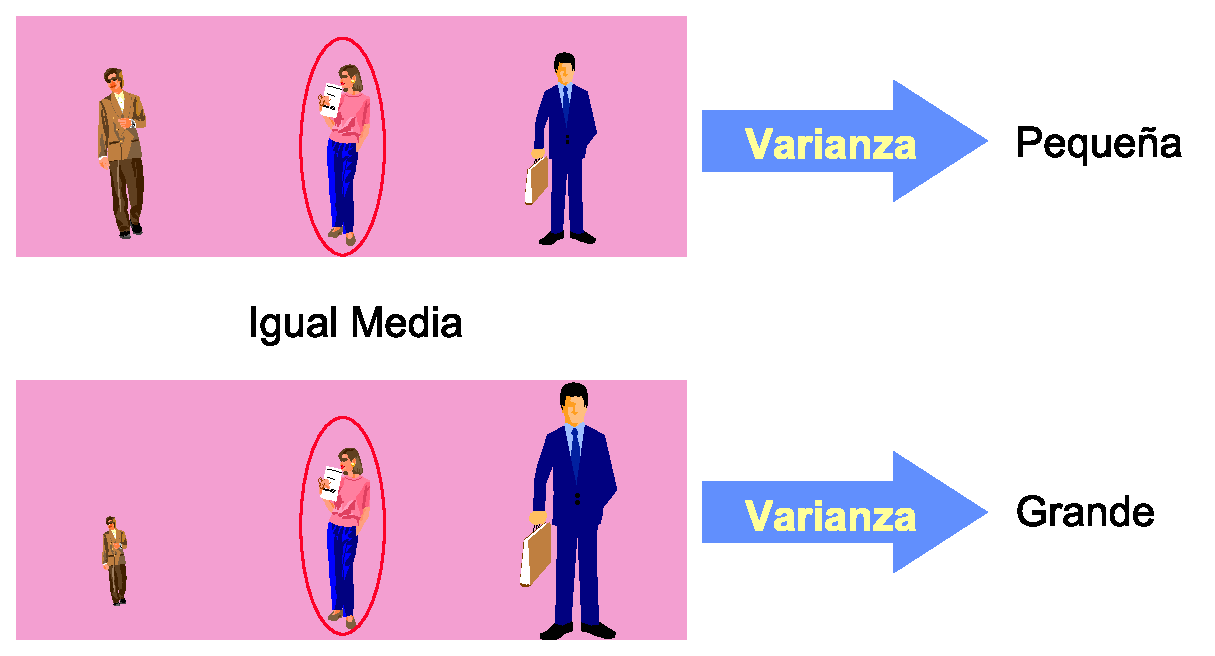
\includegraphics[scale=0.4]{img/descriptiva/interpretacion_varianza}
% 
% %\emph{¿En qué caso es más representativa la media?}
% \end{center}
% 
% \note{Tanto la varianza como la desviación típica sirven para cuantificar la dispersión de los datos en torno a la media. Si la dispersion
% con respecto a la media es pequeña, los individuos se parecerán bastante a la media y esta será más representativa que cuando los
% individuos no se parezcana ella y la dispersión con respecto a la media sea mayor.}
% \end{frame}
% 
% 
% %---------------------------------------------------------------------slide----
% \begin{frame}
% \frametitle{Cálculo de la varianza y la desviación típica}
% \framesubtitle{Ejemplo con datos no agrupados}
% Para el número de hijos se puede calcular la varianza a partir de la tabla de frecuencias añadiendo una columna con los
% cuadrados de los valores:
% \begin{center}
% \setlength\arraycolsep{3mm}
% \setlength\arrayrulewidth{0.5pt}
% \begin{array}{rrr}
% \hline
% \multicolumn{1}{c}{x_i} & \multicolumn{1}{c}{n_i} & \multicolumn{1}{c}{x_i^2n_i} \\
% \hline
% 0 & 2 & 0 \\
% 1 & 6 & 6 \\
% 2 & 14 & 56\\
% 3 & 2  & 18\\
% 4 & 1 & 16 \\ 
% \hline 
% \sum & 25 & 96 \\
% \hline
% \end{array}
% \end{center}
% \[
% s^2 = \frac{\sum x_i^2n_i}{n}-\bar x^2 = \frac{96}{25}-1.76^2= 0.7424 \mbox{ hijos}^2.
% \]
% Y la desviación típica es $s=\sqrt{0.7424} = 0.8616$ hijos.
% 
% Comparado este valor con el recorrido, que va de 0 a 4 hijos se observa que no es demasiado grande por lo que se puede concluir que no hay
% mucha dispersión y en consecuencia la media de $1.76$ hijos representa bien a los matrimonios de la muestra.
% 
% \note{En el ejemplo del número de hijos, para calcular al varianza conviene añadir una nueva columna a la tabla donde se calculen los
% productos de los cuadrados de los valores por sus frecuencias absolutas: 0 evado al cuadrado y por su frecuencia absoluta que es 2, da 0, 1
% elevado al cuadrado y por su frecuencia absoluta que es 6, que da 6, y así sucesivamente. Después hay que sumar los valores de esta
% columna y dividirlos por el tamaño de la muestra que era 25. Finalmente al cociente se le resta el valor de la media que era $1.76$
% elevada al cuadrado, lo que nos da 0.7424 hijos al cuadrado.
% 
% Si sacamos la raíz cuadrada se obtiene una desviación típica de 0.8616 hijos, que no es un valor grande comparado con el recorrido de la
% variable que va de 0 a 4 hijos, por lo que se puede concluir que la muestra no tiene mucha dispersión y por tanto la media de
% $1.76$ hijos representa muy bien a los matrimonios de la muestra.}
% \end{frame}
% 
% 
% %---------------------------------------------------------------------slide----
% \begin{frame}
% \frametitle{Cálculo de la varianza y la desviación típica}
% \framesubtitle{Ejemplo con datos agrupados}
% En el ejemplo de las estaturas, al ser datos agrupados, el cálculo se realiza igual que antes pero tomando como valores de la variable las
% marcas de clase. 
% \begin{center}
% \setlength\arraycolsep{3mm}
% \setlength\arrayrulewidth{0.5pt}
% \begin{array}{rrrr}
% \hline
% \multicolumn{1}{c}{X} & \multicolumn{1}{c}{x_i} & \multicolumn{1}{c}{n_i} & \multicolumn{1}{c}{x_i^2n_i} \\
% \hline
% (150,160] & 155 & 2 & 48050\\
% (160,170] & 165 & 8 & 217800\\
% (170,180] & 175 & 11 & 336875\\
% (180,190] & 185 & 7 & 239575\\
% (190,200] & 195 & 2 & 76050\\ 
% \hline 
% \sum &  & 30 & 918350 \\
% \hline
% \end{array}
% \end{center}
% \[
% s^2 = \frac{\sum x_i^2n_i}{n}-\bar x^2 = \frac{918350}{30}-174.67^2= 102.06 \mbox{ cm}^2.
% \]
% Y la desviación típica es $s=\sqrt{102.06} = 10.1$ cm.
% 
% Este valor es bastante pequeño, comparado con el recorrido de la variable, que va de 150 a 200 cm, por lo que la variable tiene poca
% dispersión y en consecuencia su media es muy representativa.
% 
% \note{En el ejemplo de las estaturas, como se habían agrupado los datos, como valores se tomarán las
% marcas de clases, es decir, 155 elevado al cuadrado y por su frecuencia absoluta que es 2, lo que nos da 48050, y así sucesivamente. Después
% hay que sumar los valores de esta columna y dividirlos por el tamaño de la muestra que era 30. Finalmente al cociente se le resta el valor
% de la media que era $174.67$ elevada al cuadrado, lo que nos da 102.06 cm al cuadrado.
% 
% Si sacamos la raíz cuadrada se obtiene una desviación típica de 10.1 cm, que es un valor pequeño comparado con el recorrido de la variable
% que va de 150 a 200 cm, por lo que se puede concluir que la muestra tiene poca dispersión y por tanto la media representa muy bien al resto
% de individuos de la muestra.}
% \end{frame}
% 
% 
% %---------------------------------------------------------------------slide----
% \begin{frame}
% \frametitle{Coeficiente de variación}
% Tanto la varianza como la desviación típica tienen unidades y eso dificulta a veces su interpretación y su comparación.
% 
% Afortunadamente es fácil definir a partir de ellas una medida de dispersión adimensional que es más fácil de interpretar.
% \begin{definicion}[Coeficiente de variación muestral $cv$]
% El \emph{coeficiente de variación muestral} de una variable $X$ se define como el cociente entre su desviación típica muestral y el valor absoluto de su media muestral.
% \[
% cv = \frac{s}{|\bar x|}
% \]
% \end{definicion}
% El coeficiente de variación muestral mide la dispersión relativa de los valores de la muestra en torno a la media muestral.
%  
% Como no tiene unidades, es muy sencillo de interpretar: Cuanto mayor sea, mayor será la dispersión y menos
% representativa será la media.
% 
% También se utiliza para comparar la dispersión entre muestras distintas incluso si las variables tienen unidades diferentes.
% \begin{center}
% \alert{\emph{¡Ojo! No tiene sentido cuando la media muestral vale 0 o valores próximos.}}
% \end{center}
% 
% \note{Tanto la varianza como la desviación típica tienen unidades lo que dificulta a veces su interpretación.
% 
% Afortunadamente es fácil definir a partir de ellas una medida de dispersión adimensional que es más fácil de interpretar.
% 
% El coeficiente de variación muestral, que se representa mediante cv, se defiene como el cociente entre la desviación típica y el valor
% absoluto de la media.
% 
% Como tanto la desviación típica como la media tienen las unidades de la variable, al hacer su cociente las unidades desaparecen y se obtiene
% una medida adimensional que resulta más sencilla de interpretar. 
% 
% Al estar dividido por el valor absoluto de la media, el coeficiente de variación mide la dispersión relativa de los valores de la muestra
% en torno a la media muestral, y como en el numerador está la desviación típica, cuanto mayor sea esta, mayor será el coeficiente de
% variación y por tanto mayor será la dispersión relativa de la variable en torno a la media.
% 
% Una de las principales utilidades del coeficiente de variación es que, precisamente por no tener unidades, permite la comparación de la
% dispersión de muestras distintas, incluso si son de variables con distintas unidades. 
% 
% El único problema de este estadístico es que no vale cuando la media muestral vale 0 o próxima a 0, ya que al estar en el denominador,
% obtendríamos valores muy grandes.}
% \end{frame}
% 
% 
% %---------------------------------------------------------------------slide----
% \begin{frame}
% \frametitle{Coeficiente de variación}
% \framesubtitle{Ejemplo}
% En el caso del número de hijos, como $\bar x=1.76$ hijos y $s=0.8616$ hijos, se tiene que el coefiente de variación vale
% \[
% cv = \frac{s}{|\bar x|} = \frac{0.8616}{|1.76|} = 0.49.
% \]
% En el caso de las estaturas, como $\bar x=174.67$ cm y $s=10.1$ cm, se tiene que el coeficiente de variación vale 
% \[
% cv = \frac{s}{|\bar x|} = \frac{10.1}{|174.67|} = 0.06.
% \]
% Como se puede observar la dispersión relativa en la muestra de estaturas es mucho menor que en la del número de hijos, por lo que la media
% de las estaturas será más representativa que la media del número de hijos. 
% \end{frame}
% 
% 
% \subsection{Estadísticos de forma}
% %---------------------------------------------------------------------slide----
% \begin{frame}
% \frametitle{Estadísticos de forma}
% Son medidas que tratan de caracterizar aspectos de la forma de la distribución de una muestra.
% 
% Los aspectos más relevantes son:
% \begin{description}
% \item[Simetría:] Miden la simetría de la distribución de frecuencias en torno a la media.\\
% El estadístico más utilizado es el \emph{Coeficiente de Asimetría de Fisher}.
% \item[Apuntamiento:] Miden el apuntamiento de la distribución de frecuencias.\\
% El estadístico más utilizado es el \emph{Coeficiente de Apuntamiento o Curtosis}.
% \end{description}
% \note{Los estadísticos de forma se encargan de describir, como su propio nombre indica, la forma que tiene la distribución de valores en la
% muestra, en particular se estudian dos aspectos que son la asímetría y el apuntamiento.}
% \end{frame}
% 
% 
% %---------------------------------------------------------------------slide----
% \begin{frame}
% \frametitle{Coeficiente de asimetría}
% \begin{definicion}[Coeficiente de asimetría muestral $g_1$]
% El \emph{coeficiente de asimetría muestral} de una variable $X$ se define como el promedio de las desviaciones de los
% valores de la muestra respecto de la media muestral, elevadas al cubo, dividido por la desviación típica al cubo. \[g_1
% = \frac{\sum (x_i-\bar x)^3 n_i/n}{s^3} = \frac{\sum (x_i-\bar x)^3 f_i}{s^3}\]
% \end{definicion}
% El coeficiente de asimetría muestral mide el grado de simetría de los valores de la muestra con respecto a la media muestral, de manera que:
% \begin{itemize}
% \item $g_1=0$ indica que hay el mismo número de valores a la derecha y a la izquierda de la media (simétrica).
% \item $g_1<0$ indica que la mayoría de los valores son mayores que la media (asimétrica a la izquierda).
% \item $g_1>0$ indica que la mayoría de los valores son menores que la media (asimétrica a la derecha).
% \end{itemize}
% 
% \note{La simetría con respecto a la media tiene que ver con la ubicación de los valores a un lado y otro de la media, cuántos valores hay
% por encima y cuántos por debajo, y cómo están de alejados.
% 
% El coeficiente de asimetría muestral, que se representa $g_1$ se define, como la suma del producto de las desviaciones de los valores de la
% muestra a la media muestral elevadas al cubo por su frecuencia absoluta, dividida por el tamaño de la muestra, y a su vez todo dividido
% por la desviación típica al cubo.
% 
% Como las desviaciones elevadas al cubo tienen las unidades de la variable al cubo y la desviación típica elevada al cubo también tiene las
% unidades de la variable al cubo, al realizar el cociente las unidades se cancelan y por tanto el coeficiente de asimetría es una medida
% adimensional que mide el grado de asimetría de los valores de la muestra con respecto a la media, de manera que:
% \begin{itemize}
% \item $g_1=0$ indica que hay el mismo número de valores a la derecha y a la izquierda de la media y por tanto la distribución es simétrica.
% \item $g_1<0$ indica que la mayoría de los valores son mayores que la media y entonces se dice que la distribución es asimétrica hacia la
% izquierda.
% \item $g_1>0$ indica que la mayoría de los valores son menores que la media y entonces se dice que la distribución es asimétrica hacia la
% derecha.
% \end{itemize}
% }
% \end{frame}
% 
% 
% %---------------------------------------------------------------------slide----
% \begin{frame}
% \frametitle{Coeficiente de asimetría}
% \framesubtitle{Ejemplo de distribución simétrica}
% \begin{center}
% \scalebox{0.8}{% Created by tikzDevice version 0.9 on 2015-11-20 12:10:21
% !TEX encoding = UTF-8 Unicode
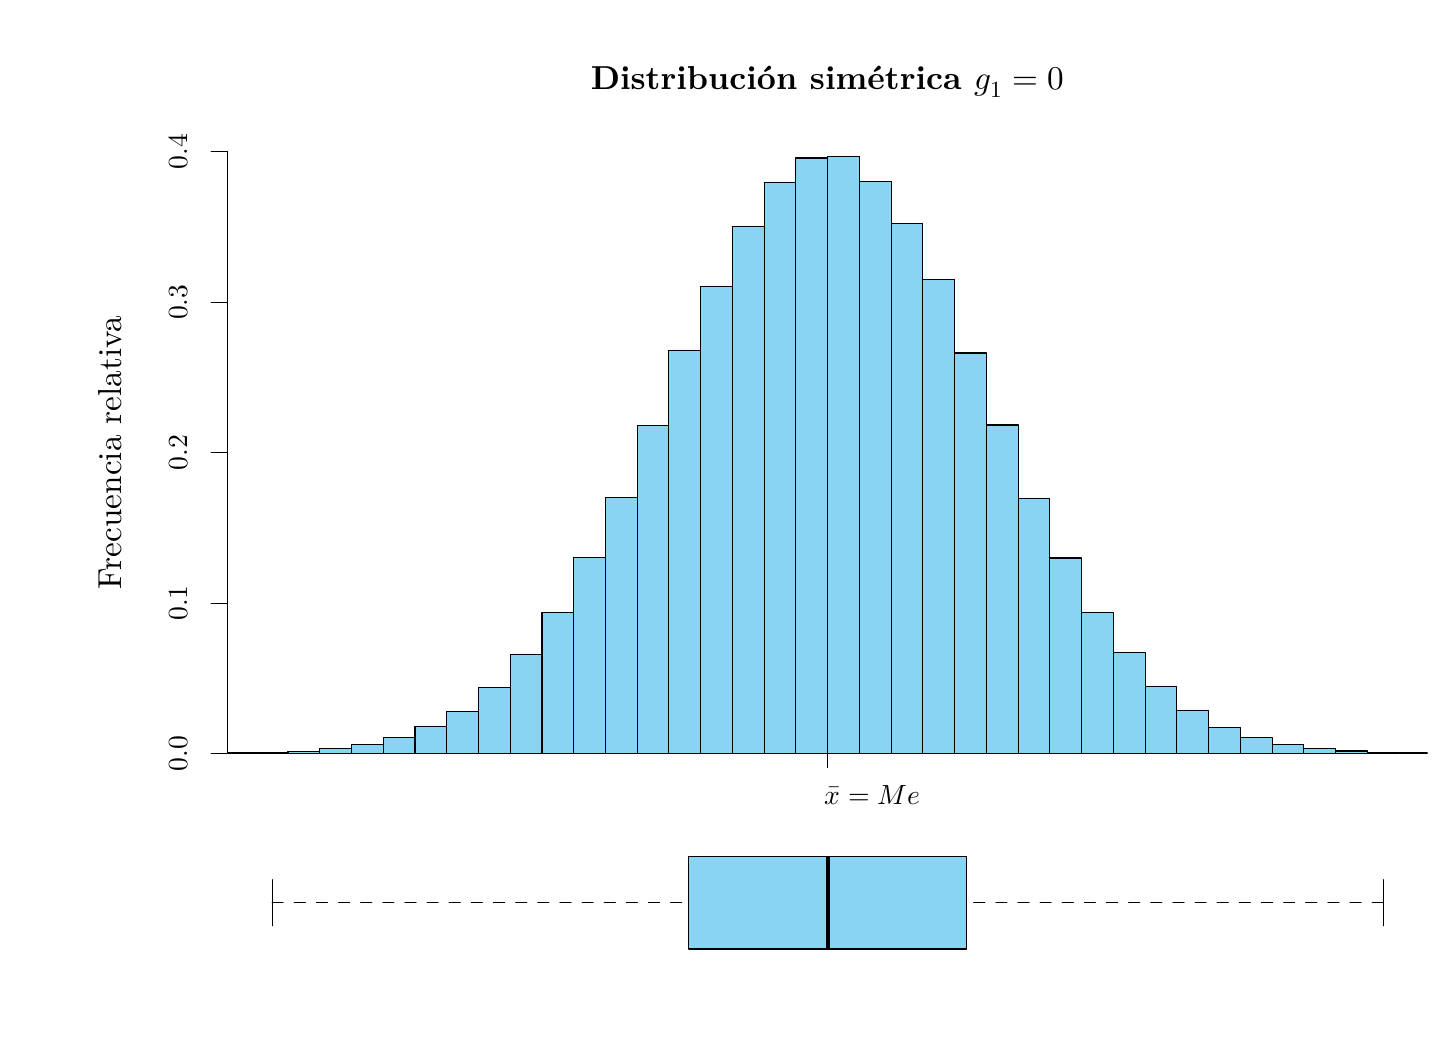
\begin{tikzpicture}[x=1pt,y=1pt]
\definecolor{fillColor}{RGB}{255,255,255}
\path[use as bounding box,fill=fillColor,fill opacity=0.00] (0,0) rectangle (505.89,361.35);
\begin{scope}
\path[clip] (  0.00, 90.34) rectangle (505.89,361.35);
\definecolor{drawColor}{RGB}{0,0,0}

\node[text=drawColor,anchor=base,inner sep=0pt, outer sep=0pt, scale=  1.20, font=\boldmath] at (289.08,339.14)
{\bfseries Distribución simétrica $g_1=0$};
 
\node[text=drawColor,rotate= 90.00,anchor=base,inner sep=0pt, outer sep=0pt, scale=  1.20] at ( 33.87,207.78) {Frecuencia relativa};
\end{scope}
\begin{scope}
\path[clip] (  0.00,  0.00) rectangle (505.89,361.35);
\definecolor{drawColor}{RGB}{0,0,0}

\path[draw=drawColor,line width= 0.4pt,line join=round,line cap=round] ( 72.27, 99.04) -- ( 72.27,316.52);

\path[draw=drawColor,line width= 0.4pt,line join=round,line cap=round] ( 72.27, 99.04) -- ( 66.27, 99.04);

\path[draw=drawColor,line width= 0.4pt,line join=round,line cap=round] ( 72.27,153.41) -- ( 66.27,153.41);

\path[draw=drawColor,line width= 0.4pt,line join=round,line cap=round] ( 72.27,207.78) -- ( 66.27,207.78);

\path[draw=drawColor,line width= 0.4pt,line join=round,line cap=round] ( 72.27,262.15) -- ( 66.27,262.15);

\path[draw=drawColor,line width= 0.4pt,line join=round,line cap=round] ( 72.27,316.52) -- ( 66.27,316.52);

\node[text=drawColor,rotate= 90.00,anchor=base,inner sep=0pt, outer sep=0pt, scale=  1.00] at ( 57.87, 99.04) {0.0};

\node[text=drawColor,rotate= 90.00,anchor=base,inner sep=0pt, outer sep=0pt, scale=  1.00] at ( 57.87,153.41) {0.1};

\node[text=drawColor,rotate= 90.00,anchor=base,inner sep=0pt, outer sep=0pt, scale=  1.00] at ( 57.87,207.78) {0.2};

\node[text=drawColor,rotate= 90.00,anchor=base,inner sep=0pt, outer sep=0pt, scale=  1.00] at ( 57.87,262.15) {0.3};

\node[text=drawColor,rotate= 90.00,anchor=base,inner sep=0pt, outer sep=0pt, scale=  1.00] at ( 57.87,316.52) {0.4};
\end{scope}
\begin{scope}
\path[clip] ( 72.27, 90.34) rectangle (505.89,325.21);
\definecolor{drawColor}{RGB}{0,0,0}
\definecolor{fillColor}{RGB}{137,211,243}

\path[draw=drawColor,line width= 0.4pt,line join=round,line cap=round,fill=fillColor] ( 13.77, 99.04) rectangle ( 25.24, 99.04);

\path[draw=drawColor,line width= 0.4pt,line join=round,line cap=round,fill=fillColor] ( 25.24, 99.04) rectangle ( 36.71, 99.05);

\path[draw=drawColor,line width= 0.4pt,line join=round,line cap=round,fill=fillColor] ( 36.71, 99.04) rectangle ( 48.18, 99.06);

\path[draw=drawColor,line width= 0.4pt,line join=round,line cap=round,fill=fillColor] ( 48.18, 99.04) rectangle ( 59.65, 99.09);

\path[draw=drawColor,line width= 0.4pt,line join=round,line cap=round,fill=fillColor] ( 59.65, 99.04) rectangle ( 71.12, 99.16);

\path[draw=drawColor,line width= 0.4pt,line join=round,line cap=round,fill=fillColor] ( 71.12, 99.04) rectangle ( 82.59, 99.30);

\path[draw=drawColor,line width= 0.4pt,line join=round,line cap=round,fill=fillColor] ( 82.59, 99.04) rectangle ( 94.07, 99.52);

\path[draw=drawColor,line width= 0.4pt,line join=round,line cap=round,fill=fillColor] ( 94.07, 99.04) rectangle (105.54, 99.95);

\path[draw=drawColor,line width= 0.4pt,line join=round,line cap=round,fill=fillColor] (105.54, 99.04) rectangle (117.01,100.89);

\path[draw=drawColor,line width= 0.4pt,line join=round,line cap=round,fill=fillColor] (117.01, 99.04) rectangle (128.48,102.31);

\path[draw=drawColor,line width= 0.4pt,line join=round,line cap=round,fill=fillColor] (128.48, 99.04) rectangle (139.95,104.82);

\path[draw=drawColor,line width= 0.4pt,line join=round,line cap=round,fill=fillColor] (139.95, 99.04) rectangle (151.42,108.79);

\path[draw=drawColor,line width= 0.4pt,line join=round,line cap=round,fill=fillColor] (151.42, 99.04) rectangle (162.89,114.39);

\path[draw=drawColor,line width= 0.4pt,line join=round,line cap=round,fill=fillColor] (162.89, 99.04) rectangle (174.37,123.01);

\path[draw=drawColor,line width= 0.4pt,line join=round,line cap=round,fill=fillColor] (174.37, 99.04) rectangle (185.84,134.71);

\path[draw=drawColor,line width= 0.4pt,line join=round,line cap=round,fill=fillColor] (185.84, 99.04) rectangle (197.31,150.13);

\path[draw=drawColor,line width= 0.4pt,line join=round,line cap=round,fill=fillColor] (197.31, 99.04) rectangle (208.78,169.74);

\path[draw=drawColor,line width= 0.4pt,line join=round,line cap=round,fill=fillColor] (208.78, 99.04) rectangle (220.25,191.61);

\path[draw=drawColor,line width= 0.4pt,line join=round,line cap=round,fill=fillColor] (220.25, 99.04) rectangle (231.72,217.53);

\path[draw=drawColor,line width= 0.4pt,line join=round,line cap=round,fill=fillColor] (231.72, 99.04) rectangle (243.19,244.61);

\path[draw=drawColor,line width= 0.4pt,line join=round,line cap=round,fill=fillColor] (243.19, 99.04) rectangle (254.67,267.97);

\path[draw=drawColor,line width= 0.4pt,line join=round,line cap=round,fill=fillColor] (254.67, 99.04) rectangle (266.14,289.65);

\path[draw=drawColor,line width= 0.4pt,line join=round,line cap=round,fill=fillColor] (266.14, 99.04) rectangle (277.61,305.28);

\path[draw=drawColor,line width= 0.4pt,line join=round,line cap=round,fill=fillColor] (277.61, 99.04) rectangle (289.08,314.26);

\path[draw=drawColor,line width= 0.4pt,line join=round,line cap=round,fill=fillColor] (289.08, 99.04) rectangle (300.55,314.91);

\path[draw=drawColor,line width= 0.4pt,line join=round,line cap=round,fill=fillColor] (300.55, 99.04) rectangle (312.02,305.72);

\path[draw=drawColor,line width= 0.4pt,line join=round,line cap=round,fill=fillColor] (312.02, 99.04) rectangle (323.49,290.70);

\path[draw=drawColor,line width= 0.4pt,line join=round,line cap=round,fill=fillColor] (323.49, 99.04) rectangle (334.97,270.37);

\path[draw=drawColor,line width= 0.4pt,line join=round,line cap=round,fill=fillColor] (334.97, 99.04) rectangle (346.44,243.80);

\path[draw=drawColor,line width= 0.4pt,line join=round,line cap=round,fill=fillColor] (346.44, 99.04) rectangle (357.91,217.79);

\path[draw=drawColor,line width= 0.4pt,line join=round,line cap=round,fill=fillColor] (357.91, 99.04) rectangle (369.38,191.33);

\path[draw=drawColor,line width= 0.4pt,line join=round,line cap=round,fill=fillColor] (369.38, 99.04) rectangle (380.85,169.70);

\path[draw=drawColor,line width= 0.4pt,line join=round,line cap=round,fill=fillColor] (380.85, 99.04) rectangle (392.32,150.03);

\path[draw=drawColor,line width= 0.4pt,line join=round,line cap=round,fill=fillColor] (392.32, 99.04) rectangle (403.79,135.51);

\path[draw=drawColor,line width= 0.4pt,line join=round,line cap=round,fill=fillColor] (403.79, 99.04) rectangle (415.27,123.17);

\path[draw=drawColor,line width= 0.4pt,line join=round,line cap=round,fill=fillColor] (415.27, 99.04) rectangle (426.74,114.54);

\path[draw=drawColor,line width= 0.4pt,line join=round,line cap=round,fill=fillColor] (426.74, 99.04) rectangle (438.21,108.56);

\path[draw=drawColor,line width= 0.4pt,line join=round,line cap=round,fill=fillColor] (438.21, 99.04) rectangle (449.68,104.81);

\path[draw=drawColor,line width= 0.4pt,line join=round,line cap=round,fill=fillColor] (449.68, 99.04) rectangle (461.15,102.37);

\path[draw=drawColor,line width= 0.4pt,line join=round,line cap=round,fill=fillColor] (461.15, 99.04) rectangle (472.62,100.87);

\path[draw=drawColor,line width= 0.4pt,line join=round,line cap=round,fill=fillColor] (472.62, 99.04) rectangle (484.09, 99.97);

\path[draw=drawColor,line width= 0.4pt,line join=round,line cap=round,fill=fillColor] (484.09, 99.04) rectangle (495.57, 99.57);

\path[draw=drawColor,line width= 0.4pt,line join=round,line cap=round,fill=fillColor] (495.57, 99.04) rectangle (507.04, 99.27);
\end{scope}
\begin{scope}
\path[clip] (  0.00,  0.00) rectangle (505.89,361.35);
\definecolor{drawColor}{RGB}{0,0,0}

\path[draw=drawColor,line width= 0.4pt,line join=round,line cap=round] (289.15, 99.04) -- (289.15, 94);

\node[text=drawColor,anchor=west,inner sep=0pt, outer sep=0pt, scale=  1.00] at (288, 84) {$\bar x=Me$};
\end{scope}
\begin{scope}
\path[clip] ( 72.27,  0.00) rectangle (505.89, 90.34);
\definecolor{fillColor}{RGB}{137,211,243}

\path[fill=fillColor] (238.87, 28.44) --
	(238.87, 61.90) --
	(339.25, 61.90) --
	(339.25, 28.44) --
	cycle;
\definecolor{drawColor}{RGB}{0,0,0}

\path[draw=drawColor,line width= 1.2pt,line join=round] (289.15, 28.44) -- (289.15, 61.90);

\path[draw=drawColor,line width= 0.4pt,dash pattern=on 4pt off 4pt ,line join=round,line cap=round] ( 88.33, 45.17) -- (238.87, 45.17);

\path[draw=drawColor,line width= 0.4pt,dash pattern=on 4pt off 4pt ,line join=round,line cap=round] (489.83, 45.17) -- (339.25, 45.17);

\path[draw=drawColor,line width= 0.4pt,line join=round,line cap=round] ( 88.33, 36.80) -- ( 88.33, 53.53);

\path[draw=drawColor,line width= 0.4pt,line join=round,line cap=round] (489.83, 36.80) -- (489.83, 53.53);

\path[draw=drawColor,line width= 0.4pt,line join=round,line cap=round] (238.87, 28.44) --
	(238.87, 61.90) --
	(339.25, 61.90) --
	(339.25, 28.44) --
	(238.87, 28.44);
\end{scope}
\end{tikzpicture}
}
% \end{center}
% \note{Aquí tenemos el histograma de una distribución simétrica. Como puede observarse, la media queda justo en el centro de la
% distribución, coincidiendo con la mediana y existe el mismo número de barras y con la misma frecuencia a un lado y a otro de la media.}
% \end{frame}
% 
% 
% %---------------------------------------------------------------------slide----
% \begin{frame}
% \frametitle{Coeficiente de asimetría}
% \framesubtitle{Ejemplo de distribución asimétrica hacia la izquierda}
% \begin{center}
% \scalebox{0.8}{%% Input file name: distribucion_asimetrica_izquierda.fig
%% FIG version: 3.2
%% Orientation: Landscape
%% Justification: Flush Left
%% Units: Inches
%% Paper size: A4
%% Magnification: 100.0
%% Resolution: 1200ppi
%% Include the following in the preamble:
%% \usepackage{textcomp}
%% End

\begin{pspicture}(5.91cm,3.25cm)(17.07cm,13.10cm)
\psset{unit=0.8cm}
%%
%% Depth: 2147483647
%%
\newrgbcolor{mycolor0}{1.00 0.50 0.31}\definecolor{mycolor0}{rgb}{1.00,0.50,0.31}
%%
%% Depth: 100
%%
\rput[l](12.07,15.54){Distribución asimétrica a la izquierda \alert{$g_1<0$}}
\rput{90}(9.68,10.89){Frecuencia relativa}
\psset{linestyle=solid,linewidth=0.03175,linecolor=black,fillstyle=none}
\psline(11.04,7.07)(11.04,14.71)
\psline(11.04,7.07)(10.83,7.07)
\psline(11.04,8.34)(10.83,8.34)
\psline(11.04,9.61)(10.83,9.61)
\psline(11.04,10.89)(10.83,10.89)
\psline(11.04,12.16)(10.83,12.16)
\psline(11.04,13.44)(10.83,13.44)
\psline(11.04,14.71)(10.83,14.71)
\rput{90}(10.53,7.07){0.00}
\rput{90}(10.53,8.34){0.02}
\rput{90}(10.53,9.61){0.04}
\rput{90}(10.53,10.89){0.06}
\rput{90}(10.53,12.16){0.08}
\rput{90}(10.53,13.44){0.10}
\rput{90}(10.53,14.71){0.12}
\psset{fillstyle=solid,fillcolor=mycolor0}
\pspolygon(10.79,7.07)(10.79,7.07)(11.42,7.07)(11.42,7.07)(10.79,7.07)
\pspolygon(11.42,7.07)(11.42,7.08)(12.04,7.08)(12.04,7.07)(11.42,7.07)
\pspolygon(12.04,7.07)(12.04,7.08)(12.67,7.08)(12.67,7.07)(12.04,7.07)
\pspolygon(12.67,7.07)(12.67,7.11)(13.30,7.11)(13.30,7.07)(12.67,7.07)
\pspolygon(13.30,7.07)(13.30,7.15)(13.92,7.15)(13.92,7.07)(13.30,7.07)
\pspolygon(13.92,7.07)(13.92,7.24)(14.55,7.24)(14.55,7.07)(13.92,7.07)
\pspolygon(14.55,7.07)(14.55,7.42)(15.18,7.42)(15.18,7.07)(14.55,7.07)
\pspolygon(15.18,7.07)(15.18,7.75)(15.81,7.75)(15.81,7.07)(15.18,7.07)
\pspolygon(15.81,7.07)(15.81,8.32)(16.43,8.32)(16.43,7.07)(15.81,7.07)
\pspolygon(16.43,7.07)(16.43,9.29)(17.06,9.29)(17.06,7.07)(16.43,7.07)
\pspolygon(17.06,7.07)(17.06,10.70)(17.69,10.70)(17.69,7.07)(17.06,7.07)
\pspolygon(17.69,7.07)(17.69,12.43)(18.31,12.43)(18.31,7.07)(17.69,7.07)
\pspolygon(18.31,7.07)(18.31,13.85)(18.94,13.85)(18.94,7.07)(18.31,7.07)
\pspolygon(18.94,7.07)(18.94,13.75)(19.57,13.75)(19.57,7.07)(18.94,7.07)
\pspolygon(19.57,7.07)(19.57,11.01)(20.20,11.01)(20.20,7.07)(19.57,7.07)
\pspolygon(20.20,7.07)(20.20,7.67)(20.82,7.67)(20.82,7.07)(20.20,7.07)
\rput[l](18.22,6.5){$\bar x$}
\psset{linewidth=0.0635,fillstyle=none}
\psline(19.34,4.58)(19.34,5.76)
\psset{linestyle=dashed,linewidth=0.03175}
\psline(17.19,5.17)(18.76,5.17)
\psline(20.82,5.17)(19.80,5.17)
\psset{linestyle=solid}
\psline(17.19,4.88)(17.19,5.47)
\psline(20.82,4.88)(20.82,5.47)
\psline(18.76,4.58)(18.76,5.76)(19.80,5.76)(19.80,4.58)(18.76,4.58)
\end{pspicture}
%% End
}
% \end{center}
% \note{En este otro caso tenemos una distribución asimétrica hacia la izquierda, donde la media queda por debajo de la mediana y las barras
% son más altas a la derecha de la media, lo que indica que hay más valores por encima de la media. Por debajo de la media habría menos
% valores, barras más bajas, pero más alejados.}
% \end{frame}
% 
% 
% %---------------------------------------------------------------------slide----
% \begin{frame}
% \frametitle{Coeficiente de asimetría}
% \framesubtitle{Ejemplo de distribución asimétrica hacia la derecha}
% \begin{center}
% \scalebox{0.8}{%% Input file name: distribucion_asimetrica_derecha.fig
%% FIG version: 3.2
%% Orientation: Landscape
%% Justification: Flush Left
%% Units: Inches
%% Paper size: A4
%% Magnification: 100.0
%% Resolution: 1200ppi
%% Include the following in the preamble:
%% \usepackage{textcomp}
%% End

\begin{pspicture}(5.91cm,3.25cm)(17.37cm,13.10cm)
\psset{unit=0.8cm}
%%
%% Depth: 2147483647
%%
\newrgbcolor{mycolor0}{1.00 0.50 0.31}\definecolor{mycolor0}{rgb}{1.00,0.50,0.31}
%%
%% Depth: 100
%%
\rput[l](12.16,15.54){Distribución asimétrica a la derecha \alert{$g_1>0$}}
\rput{90}(9.68,10.89){Frecuencia relativa}
\psset{linestyle=solid,linewidth=0.03175,linecolor=black,fillstyle=none}
\psline(11.04,7.07)(11.04,14.71)
\psline(11.04,7.07)(10.83,7.07)
\psline(11.04,8.34)(10.83,8.34)
\psline(11.04,9.61)(10.83,9.61)
\psline(11.04,10.89)(10.83,10.89)
\psline(11.04,12.16)(10.83,12.16)
\psline(11.04,13.44)(10.83,13.44)
\psline(11.04,14.71)(10.83,14.71)
\rput{90}(10.53,7.07){0.00}
\rput{90}(10.53,8.34){0.02}
\rput{90}(10.53,9.61){0.04}
\rput{90}(10.53,10.89){0.06}
\rput{90}(10.53,12.16){0.08}
\rput{90}(10.53,13.44){0.10}
\rput{90}(10.53,14.71){0.12}
\psset{fillstyle=solid,fillcolor=mycolor0}
\pspolygon(11.42,7.07)(11.42,7.67)(12.04,7.67)(12.04,7.07)(11.42,7.07)
\pspolygon(12.04,7.07)(12.04,11.02)(12.67,11.02)(12.67,7.07)(12.04,7.07)
\pspolygon(12.67,7.07)(12.67,13.76)(13.30,13.76)(13.30,7.07)(12.67,7.07)
\pspolygon(13.30,7.07)(13.30,13.85)(13.92,13.85)(13.92,7.07)(13.30,7.07)
\pspolygon(13.92,7.07)(13.92,12.43)(14.55,12.43)(14.55,7.07)(13.92,7.07)
\pspolygon(14.55,7.07)(14.55,10.70)(15.18,10.70)(15.18,7.07)(14.55,7.07)
\pspolygon(15.18,7.07)(15.18,9.29)(15.81,9.29)(15.81,7.07)(15.18,7.07)
\pspolygon(15.81,7.07)(15.81,8.32)(16.43,8.32)(16.43,7.07)(15.81,7.07)
\pspolygon(16.43,7.07)(16.43,7.74)(17.06,7.74)(17.06,7.07)(16.43,7.07)
\pspolygon(17.06,7.07)(17.06,7.41)(17.69,7.41)(17.69,7.07)(17.06,7.07)
\pspolygon(17.69,7.07)(17.69,7.24)(18.31,7.24)(18.31,7.07)(17.69,7.07)
\pspolygon(18.31,7.07)(18.31,7.15)(18.94,7.15)(18.94,7.07)(18.31,7.07)
\pspolygon(18.94,7.07)(18.94,7.11)(19.57,7.11)(19.57,7.07)(18.94,7.07)
\pspolygon(19.57,7.07)(19.57,7.09)(20.20,7.09)(20.20,7.07)(19.57,7.07)
\pspolygon(20.20,7.07)(20.20,7.07)(20.82,7.07)(20.82,7.07)(20.20,7.07)
\pspolygon(20.82,7.07)(20.82,7.07)(21.20,7.07)(21.20,7.07)(20.82,7.07)
\rput[l](13.83,6.5){$\bar x$}
\psset{linewidth=0.0635,fillstyle=none}
\psline(12.96,4.58)(12.96,5.76)
\psset{linestyle=dashed,linewidth=0.03175}
\psline(11.42,5.17)(12.47,5.17)
\psline(15.22,5.17)(13.57,5.17)
\psset{linestyle=solid}
\psline(11.42,4.88)(11.42,5.47)
\psline(15.22,4.88)(15.22,5.47)
\psline(12.47,4.58)(12.47,5.76)(13.57,5.76)(13.57,4.58)(12.47,4.58)
\end{pspicture}
%% End
}
% \end{center}
% \note{Y en este otro caso tenemos una distribución asimétrica hacia la derecha, donde la media queda por encima de la mediana y las barras
% son más altas a la izquierda de la media, lo que indica que hay más valores por debajo de la media. Por encima de la media habría menos
% valores, barras más bajas, pero más alejados.}
% \end{frame}
% 
% 
% %---------------------------------------------------------------------slide----
% \begin{frame}
% \frametitle{Cálculo del coeficiente de asimetría}
% \framesubtitle{Ejemplo con datos agrupados}
% Siguiendo con el ejemplo de las estaturas, podemos calcular el coeficiente de asimetría a partir de la tabla de frecuencias añadiendo una
% nueva columna con los cubos de las desviaciones a la media $\bar x = 174.67$ cm:
% \begin{center}
% \setlength\arraycolsep{3mm}
% \setlength\arrayrulewidth{0.5pt}
% \begin{array}{rrrrr}
% \hline
% \multicolumn{1}{c}{X} & \multicolumn{1}{c}{x_i} & \multicolumn{1}{c}{n_i} & \multicolumn{1}{c}{x_i-\bar x} & \multicolumn{1}{c}{(x_i-\bar x)^3 n_i} \\
% \hline
% (150,160] & 155 & 2 & -19.67 & -15221.00\\
% (160,170] & 165 & 8 & -9.67 & -7233.85\\
% (170,180] & 175 & 11 & 0.33 & 0.40\\
% (180,190] & 185 & 7 & 10.33 & 7716.12\\
% (190,200] & 195 & 2 & 20.33 & 16805.14\\ 
% \hline  
% \sum &  & 30 & & 2066.81 \\
% \hline
% \end{array}
% \end{center}
% \[
% g_1 = \frac{\sum (x_i-\bar x)^3n_i/n}{s^3} = \frac{2066.81/30}{10.1^3} = 0.07.
% \]
% Al estar tan próximo a 0, este valor indica que la distribución es prácticamente simétrica con respecto a la media. 
% 
% \note{Para calcular el coeficiente de asimetría en el ejemplo de las estaturas se puede añadir una nueva columna a la
% tabla de frecuencias con las desviaciones de los valores a la media que recordemos valía $174.67$ cm. Como habíamos agrupado los datos en
% clases, para calcular las desviaciones a la media se toma la marca de cada clase. Así, la primera desviación es 155 menos la media 174.67 lo
% que nos da $-19.67$ cm, la segunda es 165 menos $174.67$ cm y así sucesivamente. Obsérvese que las desviaciones de los valores menos que la
% media serán negativas y que las de los valores mayores serán positivas. A continuación se añade otra columna a la tabla con el producto de
% las desviaciones elevadas al cubo por su frecuencia absoluta, es decir, $-19.67$ al cubo por su frecuencia absoluta que es 2, lo que nos da
% $-15221$, $-9.67$ elevado al cubo y por su frecuencia absoluta que es 8, lo que nos da $-7233.85$, y así sucesivamente. Al final se suman
% los valores de esta columna y se dividen por el tamaño de la muestra que era 30. Por último el resultado de este cociente se vuelve a dividir por la desviación típica
% que era $10.1$ cm elevada al cubo, y se obtiene $0.07$.
% 
% Como este valor está muy próximo a 0, se puede concluir que la distribución de las estaturas es prácticamente simétrica.
% }
% \end{frame}
% 
% 
% %---------------------------------------------------------------------slide----
% \begin{frame}
% \frametitle{Coeficiente de apuntamiento o curtosis}
% \begin{definicion}[Coeficiente de apuntamiento muestral $g_2$]
% El \emph{coeficiente de apuntamiento muestral} de una variable $X$ se define como el promedio de las desviaciones de
% los valores de la muestra respecto de la media muestral, elevadas a la cuarta, dividido por la desviación típica a la
% cuarta y al resultado se le resta 3. \[g_2 = \frac{\sum (x_i-\bar x)^4 n_i/n}{s^4}-3 = \frac{\sum (x_i-\bar x)^4 f_i}{s^4}-3\]
% \end{definicion}
% El coeficiente de apuntamiento muestral mide el grado de apuntamiento de los valores de la muestra con respecto a una distribución normal de referencia, de manera que:
% \begin{itemize}
% \item $g_2=0$ indica que la distribución tienen un apuntamiento normal (\emph{mesocúrtica}).
% \item $g_2<0$ indica que la distribución tiene menos apuntamiento de lo normal (\emph{platicúrtica}).
% \item $g_2>0$ indica que la distribución tiene más apuntamiento de lo normal (\emph{leptocúrtica}).
% \end{itemize}
% 
% \note{El apuntamiento de una distribución muestral tiene que ver con la pendiente su polígono de frecuencias.
% 
% El coeficiente de apuntamiento o kurtosis muestral, que se representa $g_2$ se define, como la suma del producto de las desviaciones de los
% valores de la muestra a la media muestral elevadas a la cuarta por su frecuencia absoluta, dividida por el tamaño de la muestra, y a su vez
% todo dividido por la desviación típica a la cuarta, y al final se resta 3 al cociente. Como puede verse, la fórmula es muy parecida a la del
% coeficiente de asimetría, pero tomando las potencias cuartas en lugar de las potencias al cubo, y restando 3 al cociente. 
% 
% Al igual que para el coeficiente de asimetría, como las desviaciones elevadas a la cuarta tienen las unidades de la variable a la cuarta y
% la desviación típica elevada al cubo también tiene las unidades de la variable a la cuarta, al realizar el cociente las unidades se cancelan
% y por tanto el coeficiente de apuntamiento es una medida adimensional que mide el grado de apuntamiento de la distribución muestral.
% 
% El apuntamiento suele medirse en comparación con un apuntamiento de referencia que es el de una distribución normal. La distribución normal
% se verá maś adelante en el curso, pero baste decir que es la distribución más común que se presenta en la naturaleza, y por lo tanto, está
% justificado tomarla como referencia y comparar el apuntamiento de cualquier otra distribución con el de la distribución normal que siempre
% vale 0. Por tanto cuando
% \begin{itemize}
% \item $g_2=0$ indica que la distribución tienen un apuntamiento normal (\emph{mesocúrtica}).
% \item $g_2<0$ indica que la distribución tiene menos apuntamiento de lo normal (\emph{platicúrtica}).
% \item $g_2>0$ indica que la distribución tiene más apuntamiento de lo normal (\emph{leptocúrtica}
% \end{itemize}
% }
% \end{frame}
% 
% 
% %---------------------------------------------------------------------slide----
% \begin{frame}
% \frametitle{Coeficiente de apuntamiento o curtosis}
% \framesubtitle{Ejemplo de distribución mesocúrtica}
% \begin{center}
% \scalebox{0.8}{%% Input file name: distribucion_mesocurtica.fig
%% FIG version: 3.2
%% Orientation: Landscape
%% Justification: Flush Left
%% Units: Inches
%% Paper size: A4
%% Magnification: 100.0
%% Resolution: 1200ppi
%% Include the following in the preamble:
%% \usepackage{textcomp}
%% End

\begin{pspicture}(5.26cm,3.44cm)(16.90cm,11.91cm)
\psset{unit=0.8cm}
%%
%% Depth: 2147483647
%%
\newrgbcolor{mycolor0}{1.00 0.50 0.31}\definecolor{mycolor0}{rgb}{1.00,0.50,0.31}
\newrgbcolor{mycolor1}{0.25 0.41 0.88}\definecolor{mycolor1}{rgb}{0.25,0.41,0.88}
%%
%% Depth: 100
%%
\rput[l](12.46,14.06){Distribución mesocúrtica \alert{$g_2=0$}}
\rput{90}(8.88,8.89){Frecuencia relativa}
\psset{linestyle=solid,linewidth=0.03175,linecolor=black,fillstyle=solid,fillcolor=mycolor0}
\pspolygon(9.94,4.82)(9.94,4.83)(10.61,4.83)(10.61,4.82)(9.94,4.82)
\pspolygon(10.61,4.82)(10.61,4.87)(11.27,4.87)(11.27,4.82)(10.61,4.82)
\pspolygon(11.27,4.82)(11.27,5.01)(11.94,5.01)(11.94,4.82)(11.27,4.82)
\pspolygon(11.94,4.82)(11.94,5.49)(12.61,5.49)(12.61,4.82)(11.94,4.82)
\pspolygon(12.61,4.82)(12.61,6.60)(13.27,6.60)(13.27,4.82)(12.61,4.82)
\pspolygon(13.27,4.82)(13.27,8.57)(13.94,8.57)(13.94,4.82)(13.27,4.82)
\pspolygon(13.94,4.82)(13.94,10.92)(14.61,10.92)(14.61,4.82)(13.94,4.82)
\pspolygon(14.61,4.82)(14.61,12.63)(15.27,12.63)(15.27,4.82)(14.61,4.82)
\pspolygon(15.27,4.82)(15.27,12.64)(15.94,12.64)(15.94,4.82)(15.27,4.82)
\pspolygon(15.94,4.82)(15.94,10.93)(16.61,10.93)(16.61,4.82)(15.94,4.82)
\pspolygon(16.61,4.82)(16.61,8.55)(17.27,8.55)(17.27,4.82)(16.61,4.82)
\pspolygon(17.27,4.82)(17.27,6.61)(17.94,6.61)(17.94,4.82)(17.27,4.82)
\pspolygon(17.94,4.82)(17.94,5.49)(18.60,5.49)(18.60,4.82)(17.94,4.82)
\pspolygon(18.60,4.82)(18.60,5.02)(19.27,5.02)(19.27,4.82)(18.60,4.82)
\pspolygon(19.27,4.82)(19.27,4.86)(19.94,4.86)(19.94,4.82)(19.27,4.82)
\pspolygon(19.94,4.82)(19.94,4.83)(20.60,4.83)(20.60,4.82)(19.94,4.82)
\psset{fillstyle=none}
\psline(10.23,4.82)(10.23,12.97)
\psline(10.23,4.82)(10.02,4.82)
\psline(10.23,6.86)(10.02,6.86)
\psline(10.23,8.89)(10.02,8.89)
\psline(10.23,10.93)(10.02,10.93)
\psline(10.23,12.97)(10.02,12.97)
\rput{90}(9.73,4.82){0.0}
\rput{90}(9.73,6.86){0.1}
\rput{90}(9.73,8.89){0.2}
\rput{90}(9.73,10.93){0.3}
\rput{90}(9.73,12.97){0.4}
\psset{linewidth=0.0635,linecolor=mycolor1}
\psline(10.61,4.84)(10.70,4.84)(10.79,4.85)(10.89,4.85)(10.98,4.86)(11.07,4.87)(11.17,4.89)(11.26,4.91)(11.35,4.93)(11.45,4.95)(11.54,4.98)(11.63,5.01)(11.73,5.05)(11.82,5.10)(11.91,5.16)(12.01,5.22)(12.10,5.30)(12.19,5.38)(12.29,5.48)(12.38,5.59)(12.47,5.71)(12.57,5.85)(12.66,6.01)(12.75,6.18)(12.85,6.37)(12.94,6.58)(13.03,6.80)(13.13,7.04)(13.22,7.30)(13.31,7.58)(13.41,7.87)(13.50,8.18)(13.59,8.49)(13.69,8.82)(13.78,9.16)(13.87,9.50)(13.97,9.85)(14.06,10.19)(14.15,10.53)(14.25,10.86)(14.34,11.18)(14.43,11.49)(14.53,11.77)(14.62,12.03)(14.71,12.26)(14.81,12.47)(14.90,12.64)(14.99,12.77)(15.09,12.87)(15.18,12.93)(15.27,12.95)(15.36,12.93)(15.46,12.87)(15.55,12.77)(15.65,12.64)(15.74,12.47)(15.83,12.26)(15.93,12.03)(16.02,11.77)(16.11,11.49)(16.21,11.18)(16.30,10.86)(16.39,10.53)(16.48,10.19)(16.58,9.85)(16.67,9.50)(16.77,9.16)(16.86,8.82)(16.95,8.49)(17.05,8.18)(17.14,7.87)(17.23,7.58)(17.32,7.30)(17.42,7.04)(17.51,6.80)(17.60,6.58)(17.70,6.37)(17.79,6.18)(17.88,6.01)(17.98,5.85)(18.07,5.71)(18.17,5.59)(18.26,5.48)(18.35,5.38)(18.44,5.30)(18.54,5.22)(18.63,5.16)(18.72,5.10)(18.82,5.05)(18.91,5.01)(19.00,4.98)(19.10,4.95)(19.19,4.93)(19.28,4.91)(19.38,4.89)(19.47,4.87)(19.56,4.86)(19.66,4.85)(19.75,4.85)(19.84,4.84)(19.94,4.84)
\end{pspicture}
%% End
}
% \end{center}
% \note{Aquí un histograma con coeficente de apuntamiento 0 y sobre él una distribución normal, representada por esta curva conocida
% como campana de Gauss. Obsérvese cómo la altura de las barras coinciden con la campaña de Gauss y se ajustan perfectamente a la
% distribución normal, lo que indica que la distribución es mesocúrtica.}
% \end{frame}
% 
% 
% %---------------------------------------------------------------------slide----
% \begin{frame}
% \frametitle{Coeficiente de apuntamiento o curtosis}
% \framesubtitle{Ejemplo de distribución platicúrtica}
% \begin{center}
% \scalebox{0.8}{%% Input file name: distribucion_platicurtica.fig
%% FIG version: 3.2
%% Orientation: Landscape
%% Justification: Flush Left
%% Units: Inches
%% Paper size: A4
%% Magnification: 100.0
%% Resolution: 1200ppi
%% Include the following in the preamble:
%% \usepackage{textcomp}
%% End

\begin{pspicture}(5.50cm,3.44cm)(16.66cm,11.91cm)
\psset{unit=0.8cm}
%%
%% Depth: 2147483647
%%
\newrgbcolor{mycolor0}{1.00 0.50 0.31}\definecolor{mycolor0}{rgb}{1.00,0.50,0.31}
\newrgbcolor{mycolor1}{0.25 0.41 0.88}\definecolor{mycolor1}{rgb}{0.25,0.41,0.88}
%%
%% Depth: 100
%%
\rput[l](12.50,14.06){Distribución platicúrtica \alert{$g_2<0$}}
\rput{90}(8.88,8.89){Frecuencia relativa}
\psset{linestyle=solid,linewidth=0.03175,linecolor=black,fillstyle=solid,fillcolor=mycolor0}
\pspolygon(10.61,4.82)(10.61,7.31)(11.39,7.31)(11.39,4.82)(10.61,4.82)
\pspolygon(11.39,4.82)(11.39,7.41)(12.16,7.41)(12.16,4.82)(11.39,4.82)
\pspolygon(12.16,4.82)(12.16,7.79)(12.94,7.79)(12.94,4.82)(12.16,4.82)
\pspolygon(12.94,4.82)(12.94,8.10)(13.72,8.10)(13.72,4.82)(12.94,4.82)
\pspolygon(13.72,4.82)(13.72,8.93)(14.49,8.93)(14.49,4.82)(13.72,4.82)
\pspolygon(14.49,4.82)(14.49,9.73)(15.27,9.73)(15.27,4.82)(14.49,4.82)
\pspolygon(15.27,4.82)(15.27,9.46)(16.05,9.46)(16.05,4.82)(15.27,4.82)
\pspolygon(16.05,4.82)(16.05,9.02)(16.83,9.02)(16.83,4.82)(16.05,4.82)
\pspolygon(16.83,4.82)(16.83,8.26)(17.60,8.26)(17.60,4.82)(16.83,4.82)
\pspolygon(17.60,4.82)(17.60,7.79)(18.38,7.79)(18.38,4.82)(17.60,4.82)
\pspolygon(18.38,4.82)(18.38,7.53)(19.16,7.53)(19.16,4.82)(18.38,4.82)
\pspolygon(19.16,4.82)(19.16,7.28)(19.94,7.28)(19.94,4.82)(19.16,4.82)
\psset{fillstyle=none}
\psline(10.23,4.82)(10.23,12.97)
\psline(10.23,4.82)(10.02,4.82)
\psline(10.23,6.86)(10.02,6.86)
\psline(10.23,8.89)(10.02,8.89)
\psline(10.23,10.93)(10.02,10.93)
\psline(10.23,12.97)(10.02,12.97)
\rput{90}(9.73,4.82){0.0}
\rput{90}(9.73,6.86){0.1}
\rput{90}(9.73,8.89){0.2}
\rput{90}(9.73,10.93){0.3}
\rput{90}(9.73,12.97){0.4}
\psset{linewidth=0.0635,linecolor=mycolor1}
\psline(10.23,4.86)(10.27,4.86)(10.37,4.87)(10.48,4.89)(10.59,4.91)(10.70,4.93)(10.81,4.95)(10.92,4.98)(11.03,5.01)(11.14,5.05)(11.25,5.10)(11.35,5.16)(11.46,5.22)(11.57,5.30)(11.68,5.38)(11.79,5.48)(11.90,5.59)(12.01,5.71)(12.12,5.85)(12.23,6.01)(12.33,6.18)(12.44,6.37)(12.55,6.58)(12.66,6.80)(12.77,7.04)(12.88,7.30)(12.99,7.58)(13.10,7.87)(13.20,8.18)(13.31,8.49)(13.42,8.82)(13.53,9.16)(13.64,9.50)(13.75,9.85)(13.86,10.19)(13.97,10.53)(14.08,10.86)(14.18,11.18)(14.29,11.49)(14.40,11.77)(14.51,12.03)(14.62,12.26)(14.73,12.47)(14.84,12.64)(14.95,12.77)(15.06,12.87)(15.16,12.93)(15.27,12.95)(15.38,12.93)(15.49,12.87)(15.60,12.77)(15.71,12.64)(15.82,12.47)(15.93,12.26)(16.03,12.03)(16.14,11.77)(16.25,11.49)(16.36,11.18)(16.47,10.86)(16.58,10.53)(16.69,10.19)(16.80,9.85)(16.91,9.50)(17.01,9.16)(17.12,8.82)(17.23,8.49)(17.34,8.18)(17.45,7.87)(17.56,7.58)(17.67,7.30)(17.78,7.04)(17.88,6.80)(17.99,6.58)(18.10,6.37)(18.21,6.18)(18.32,6.01)(18.43,5.85)(18.54,5.71)(18.65,5.59)(18.76,5.48)(18.86,5.38)(18.97,5.30)(19.08,5.22)(19.19,5.16)(19.30,5.10)(19.41,5.05)(19.52,5.01)(19.63,4.98)(19.74,4.95)(19.84,4.93)(19.95,4.91)(20.06,4.89)(20.17,4.87)(20.28,4.86)(20.31,4.86)
\end{pspicture}
%% End
}
% \end{center}
% \note{Ahora tenemos un histograma con un coeficiente de apuntamiento menor que 0. Como se puede apreciar, en este caso la altura de las
% barras centrales están por debajo de la campa de Gauss y la distribución tiene menos apuntamiento de lo normal, por lo que se dice que es
% platicúrtica.}
% \end{frame}
% 
% 
% %---------------------------------------------------------------------slide----
% \begin{frame}
% \frametitle{Coeficiente de apuntamiento o curtosis}
% \framesubtitle{Ejemplo de distribución leptocúrtica}
% \begin{center}
% \scalebox{0.8}{%% Input file name: distribucion_leptocurtica.fig
%% FIG version: 3.2
%% Orientation: Landscape
%% Justification: Flush Left
%% Units: Inches
%% Paper size: A4
%% Magnification: 100.0
%% Resolution: 1200ppi
%% Include the following in the preamble:
%% \usepackage{textcomp}
%% End

\begin{pspicture}(5.50cm,3.44cm)(16.66cm,11.91cm)
\psset{unit=0.8cm}
%%
%% Depth: 2147483647
%%
\newrgbcolor{mycolor0}{1.00 0.50 0.31}\definecolor{mycolor0}{rgb}{1.00,0.50,0.31}
\newrgbcolor{mycolor1}{0.25 0.41 0.88}\definecolor{mycolor1}{rgb}{0.25,0.41,0.88}
%%
%% Depth: 100
%%
\rput[l](12.43,14.06){Distribución leptocúrtica \alert{$g_2>0$}}
\rput{90}(8.88,8.89){Frecuencia relativa}
\psset{linestyle=solid,linewidth=0.03175,linecolor=black,fillstyle=solid,fillcolor=mycolor0}
\pspolygon(10.61,4.82)(10.61,4.94)(11.39,4.94)(11.39,4.82)(10.61,4.82)
\pspolygon(11.39,4.82)(11.39,5.10)(12.16,5.10)(12.16,4.82)(11.39,4.82)
\pspolygon(12.16,4.82)(12.16,5.31)(12.94,5.31)(12.94,4.82)(12.16,4.82)
\pspolygon(12.94,4.82)(12.94,6.26)(13.72,6.26)(13.72,4.82)(12.94,4.82)
\pspolygon(13.72,4.82)(13.72,8.14)(14.49,8.14)(14.49,4.82)(13.72,4.82)
\pspolygon(14.49,4.82)(14.49,12.64)(15.27,12.64)(15.27,4.82)(14.49,4.82)
\pspolygon(15.27,4.82)(15.27,12.86)(16.05,12.86)(16.05,4.82)(15.27,4.82)
\pspolygon(16.05,4.82)(16.05,8.19)(16.83,8.19)(16.83,4.82)(16.05,4.82)
\pspolygon(16.83,4.82)(16.83,6.18)(17.60,6.18)(17.60,4.82)(16.83,4.82)
\pspolygon(17.60,4.82)(17.60,5.32)(18.38,5.32)(18.38,4.82)(17.60,4.82)
\pspolygon(18.38,4.82)(18.38,5.08)(19.16,5.08)(19.16,4.82)(18.38,4.82)
\pspolygon(19.16,4.82)(19.16,4.98)(19.94,4.98)(19.94,4.82)(19.16,4.82)
\psset{fillstyle=none}
\psline(10.23,4.82)(10.23,12.97)
\psline(10.23,4.82)(10.02,4.82)
\psline(10.23,6.18)(10.02,6.18)
\psline(10.23,7.54)(10.02,7.54)
\psline(10.23,8.89)(10.02,8.89)
\psline(10.23,10.25)(10.02,10.25)
\psline(10.23,11.61)(10.02,11.61)
\psline(10.23,12.97)(10.02,12.97)
\rput{90}(9.73,4.82){0.0}
\rput{90}(9.73,6.18){0.1}
\rput{90}(9.73,7.54){0.2}
\rput{90}(9.73,8.89){0.3}
\rput{90}(9.73,10.25){0.4}
\rput{90}(9.73,11.61){0.5}
\rput{90}(9.73,12.97){0.6}
\psset{linewidth=0.0635,linecolor=mycolor1}
\psline(10.23,4.85)(10.27,4.85)(10.37,4.86)(10.48,4.87)(10.59,4.88)(10.70,4.89)(10.81,4.91)(10.92,4.93)(11.03,4.95)(11.14,4.98)(11.25,5.01)(11.35,5.04)(11.46,5.09)(11.57,5.14)(11.68,5.19)(11.79,5.26)(11.90,5.33)(12.01,5.42)(12.12,5.51)(12.23,5.61)(12.33,5.73)(12.44,5.85)(12.55,5.99)(12.66,6.14)(12.77,6.30)(12.88,6.47)(12.99,6.66)(13.10,6.85)(13.20,7.06)(13.31,7.27)(13.42,7.49)(13.53,7.71)(13.64,7.94)(13.75,8.17)(13.86,8.40)(13.97,8.63)(14.08,8.85)(14.18,9.06)(14.29,9.26)(14.40,9.45)(14.51,9.63)(14.62,9.78)(14.73,9.92)(14.84,10.03)(14.95,10.12)(15.06,10.19)(15.16,10.23)(15.27,10.24)(15.38,10.23)(15.49,10.19)(15.60,10.12)(15.71,10.03)(15.82,9.92)(15.93,9.78)(16.03,9.63)(16.14,9.45)(16.25,9.26)(16.36,9.06)(16.47,8.85)(16.58,8.63)(16.69,8.40)(16.80,8.17)(16.91,7.94)(17.01,7.71)(17.12,7.49)(17.23,7.27)(17.34,7.06)(17.45,6.85)(17.56,6.66)(17.67,6.47)(17.78,6.30)(17.88,6.14)(17.99,5.99)(18.10,5.85)(18.21,5.73)(18.32,5.61)(18.43,5.51)(18.54,5.42)(18.65,5.33)(18.76,5.26)(18.86,5.19)(18.97,5.14)(19.08,5.09)(19.19,5.04)(19.30,5.01)(19.41,4.98)(19.52,4.95)(19.63,4.93)(19.74,4.91)(19.84,4.89)(19.95,4.88)(20.06,4.87)(20.17,4.86)(20.28,4.85)(20.31,4.85)
\end{pspicture}
%% End
}
% \end{center}
% \note{En este otro caso tenemos un histograma con un coeficiente de apuntamiento mayor que 0. Ahora la altura
% de las barras centrales están por encima de la campa de Gauss y la distribución tiene más apuntamiento de lo normal, por lo que se dice
% que es leptocúrtica.}
% \end{frame}
% 
% 
% %---------------------------------------------------------------------slide----
% \begin{frame}
% \frametitle{Cálculo del coeficiente de apuntamiento}
% \framesubtitle{Ejemplo con datos agrupados}
% De nuevo para el ejemplo de las estaturas podemos calcular el coeficiente de asimetría a partir de la tabla de frecuencias añadiendo una
% nueva columna con las desviaciones a la media $\bar x = 174.67$ cm elevadas a la cuarta: 
% \begin{center}
% \setlength\arraycolsep{3mm}
% \setlength\arrayrulewidth{0.5pt}
% \begin{array}{rrrrr}
% \hline
% \multicolumn{1}{c}{X} & \multicolumn{1}{c}{x_i} & \multicolumn{1}{c}{n_i} & \multicolumn{1}{c}{x_i-\bar x} & \multicolumn{1}{c}{(x_i-\bar x)^4 n_i} \\
% \hline
% (150,160] & 155 & 2 & -19.67 & 299396.99\\
% (160,170] & 165 & 8 & -9.67 & 69951.31\\
% (170,180] & 175 & 11 & 0.33 & 0.13\\
% (180,190] & 185 & 7 & 10.33 & 79707.53\\
% (190,200] & 195 & 2 & 20.33 & 341648.49\\ 
% \hline 
% \sum &  & 30 & & 790704.45 \\
% \hline
% \end{array}
% \end{center}
% \[
% g_2 = \frac{\sum (x_i-\bar x)^4n_i/n}{s^4} - 3 = \frac{790704.45/30}{10.1^4}-3 = -0.47.
% \]
% Como se trata de un valor negativo, aunque pequeño, podemos decir que la distribución es ligeramente platicúrtica. 
% 
% \note{El coeficiente de apuntamiento se calcula de manera similar al coeficiente de asimetría, calculando primero las desviaciones a la
% meida en una columna de la tabla y luego añadiendo otra columna con el producto de
% las desviaciones elevadas a la cuarta por su frecuencia absoluta, es decir, $-19.67$ a la cuarta por su frecuencia absoluta que es 2, lo que
% nos da $299396.99$, $-9.67$ elevado a la cuarta y por su frecuencia absoluta que es 8, lo que nos da $69951.31$, y así sucesivamente. Al
% final se suman los valores de esta columna y se dividen por el tamaño de la muestra que era 30. Por último el resultado de este cociente se
% vuelve a dividir por la desviación típica que era $10.1$ cm elevada a la cuarta, y al resultado se le resta 3, obteniendo -0.47.
% 
% Como se trata de un valor negativo, aunque próximo a cero, se puede concluir que la distribución de las estaturas es ligeramente
% platicúrtica. }
% \end{frame}
% 
% 
% %---------------------------------------------------------------------slide----
% \begin{frame}
% \frametitle{Interpretación de los coeficientes de asimetría y apuntamiento}
% Como se verá más adelante en la parte de inferencia, muchas de las pruebas estadísticas solo pueden aplicarse a poblaciones normales.
% 
% Las poblaciones normales se caracterizan por ser simétricas y mesocúrticas, de manera que, tanto el coeficiente de asimetría como el de apuntamiento pueden utilizarse para contrastar si los datos de la muestra provienen de una población normal.
% 
% En general, se suele rechazar la hipótesis de normalidad de la población cuando $g_1$ o $g_2$ estén fuera del intervalo $[-2,2]$.
% 
% En tal caso, lo habitual es aplicar alguna transformación a la variable para corregir la anormalidad.
% 
% \note{Como se verá más adelante en la parte de inferencia, muchas de las pruebas estadísticas solo pueden aplicarse a poblaciones normales,
% que se caracterizan por ser simétricas y mesocúrticas, de manera que, tanto el coeficiente de asimetría como el de apuntamiento pueden
% utilizarse para comprobar si los datos de la muestra provienen de una población normal. 
% 
% En general, se suele rechazar la hipótesis de normalidad de la población cuando $g_1$ o $g_2$ estén fuera del intervalo $[-2,2]$.
% 
% En tal caso, lo habitual es aplicar alguna transformación a la variable para corregir la anormalidad.
% }
% \end{frame}
% 
% 
% \subsection{Transformaciones de variables}
% 
% %---------------------------------------------------------------------slide----
% \begin{frame}
% \frametitle{Transformaciones de variables}
% En muchas ocasiones se suelen transformar los datos brutos para trabajar con unas unidades más cómodas, o bien para corregir alguna
% anormalidad de la distribución.
% 
% 
% Por ejemplo, si estamos trabajando con estaturas medidas en metros y tenemos los siguientes valores:
% \[ 
% 1.75\mbox{m}, 1.65\mbox{m}, 1.80\mbox{m},
% \]
% podemos evitar los decimales multiplicando por 100, es decir, pasando de metros a centímetros:
% \[ 
% 175\mbox{cm}, 165\mbox{cm}, 180\mbox{cm},
% \]
% Y si queremos reducir la magnitud de los datos podemos restarles a todos el menor de ellos, en este caso, 165cm:
% \[ 
% 10\mbox{cm}, 0\mbox{cm}, 15\mbox{cm},
% \]
% Está claro que este conjunto de datos es mucho más sencillo que el original. En el fondo lo que se ha hecho es aplicar a los datos la
% transformación: \[Y= 100X-165\]
% 
% \note{En muchas ocasiones los datos brutos de la muestra suelen transformarse, a veces simplemente para cambiar a una escala más cómoda y
% otras veces para corregir alguna anormalidad de la distribución.
% 
% Si por ejemplo estamos trabajando con estaturas medidas en metros, con dos decimales como los de este ejemplo, podemos evitar el trabajo
% con decimales multiplicando por 100, es decir, pasando de metros a centímetros. Así tenemos que $1.75$ m multiplicado por 100 se transforma
% en 175 cm, $1.65$ m multiplicado por 100 se trasnforma en 165 cm y $1.80$ m se transforma en 180 cm.
% 
% Después, si queremos reducir la magnitud de los datos y pasar de centenas a unidades más pequeñas, podemos restarle a todos los datos el
% mínimo de los valores que es 165 cm. 175 cm menos 165 cm nos da 10 cm, 165 menos 165 nos da 0 cm y 180 menos 165 nos da 15 cm.
% 
% Con esto los datos pasan a una escala mucho más fácil de manejar que la original. En el fondo lo que hemos hecho es aplicar a cada dato la
% transformación lineal $Y=100x-165$.}
% \end{frame}
% 
% 
% %---------------------------------------------------------------------slide----
% \begin{frame}
% \frametitle{Transformaciones lineales}
% Una de las transformaciones más habituales es la \emph{transformación lineal}:
% \[
% Y=a+bX.
% \]
% Se puede comprobar fácilmente que la media y la desviación típica de la variable resultante cumplen:
% \begin{align*}
% \bar y &= a+ b\bar x,\\
% s_{y} &= |b|s_{x}
% \end{align*}
% Además, el coeficiente de curtosis no se altera y el de asimetría sólo cambia de signo si $b$ es negativo.
% 
% \note{Una de las transformaciones más habituales que suele realizarse es la \emph{transformación lineal} que sigue la ecuación de una recta
% $Y=a+bX$, donde $a$ es el término independiente y $b$ la pendiente de la recta.
% 
% Una propiedad que tiene esta transformación y resulta fácil de comprobar es que la media de la variable transformada se puede obtener
% aplicando la misma transformación lineal a la media de la variable original, es decir, $\bar y = a+ b\bar x$, y por otro lado, la desviación
% típica de la variable transformada se puede obtener multiplicando la desviación típica de la variable original por el valor absoluto de la
% pendiente de la trasnformación lineal, es decir,  $s_{y} &= |b|s_{x}$.
% 
% Además, el coeficiente de curtosis no se altera y el de asimetría sólo cambia de signo si la pendiente es negativa.
% }
% \end{frame}
% 
% 
% %---------------------------------------------------------------------slide----
% \begin{frame}
% \frametitle{Transformación de tipificación y puntuaciones típicas}
% Una de las transformaciones lineales más habituales es la \emph{tipificación}:
% \begin{definicion}[Variable tipificada]
% La \emph{variable tipificada} de una variable estadística $X$ es la variable que resulta de restarle su media y dividir por su desviación típica.
% \[
% Z=\frac{X-\bar x}{s_{x}}
% \]
% \end{definicion}
% 
% La tipificación es muy útil para eliminar la dependencia de una variable respecto de las unidades de medida empleadas.
% 
% Los valores tipificados se conocen como \highlight{\textbf{puntuaciones típicas}} y miden el número de desviaciones típicas que dista de la media cada observación, lo cual es útil para comparar variables con distintas unidades. 
% 
% Otra propiedad de la variable tipificada es que tiene media 0 y desviación típica 1:
% \[
% \bar z = 0 \qquad s_{z} = 1
% \]
% 
% \note{Entre las transformaciones lineales hay una de especial importancia, y se conoce como transformación de tipificación. La tipificación
% consiste en dividir las desviaciones de los valores a la media por la desviación típica. 
% 
% Como las desviaciones a la media tienen las unidades de la variable y la desviación típica también, al hacer el cociente se cancelan las
% unidades y los valores de la variable tipificada no tienen unidades, por lo que esta transformación es útil para eliminar la dependencia de
% la variable de las unidades de medida empleadas.
% 
% Los valores tipificados se conocen como \highlight{\textbf{puntuaciones típicas}} y miden el número de desviaciones típicas que dista de la
% media cada observación, lo cual es útil para comparar variables con distintas unidades.
% 
% Otra propiedad que se deduce de las propiedades de las trasnformaciones lineales vistas antes es que la media de una variable tipificada
% siempre vale 0 y su desviación típica 1.
% }
% \end{frame}
% 
% 
% %---------------------------------------------------------------------slide----
% \begin{frame}
% \frametitle{Transformación de tipificación y puntuaciones típicas}
% \framesubtitle{Ejemplo}
% Las notas de 5 alumnos en dos asignaturas $X$ e $Y$ son:
% \[
% \begin{array}{rccccccccc}
% \mbox{Alumno:} & 1 & 2 & 3 & 4 & 5\\ \cline{1-6}
% X: & 2 & 5 & 4 & \alert{8} & 6 & \qquad & \bar x = 5 & \quad s_x = 2\\
% Y: & 1 & 9 & \alert{8} & 5 & 2 & \qquad & \bar y = 5 & \quad s_y = 3.16\\
% \end{array}
% \]
% \begin{center}
% \emph{¿Han tenido el mismo rendimiento los alumnos que han sacado un 8?}
% \end{center}
% Podría parecer que ambos alumnos han tenido el mismo rendimiento puesto que tienen la misma nota, pero si queremos ver el rendimiento relativo al resto del grupo, tendríamos que tener en cuenta la dispersión de cada muestra y medir sus puntuaciones típicas:
% \[
% \begin{array}{cccccc}
% X: & -1.5 & 0 & -0.5 & \alert{1.5} & 0.5 \\
% Y: & -1.26 & 1.26 & \alert{0.95} & 0 & -0.95\\
% \end{array}
% \]
% Es decir, el alumno que tiene un 8 en $X$ está $1.5$ veces la desviación típica por encima de la media de su grupo, mientras que el alumno que tiene un 8 en $Y$ sólo está $0.95$ desviaciones típicas por encima de su media.
% Así pues, el primer alumno tuvo un rendimiento superior al segundo. 
% 
% \note{Para ver la utilidad de la transformación de tipificación, supongamos que tenemos un grupo de 5 alumnos en los que se ha medido la
% nota en dos asignaturas $X$ e $Y$. Si calculamos la media y la desviación típica en cada asignatura, se tiene que la nota media en $X$ es
% 5 con una desviación típica de $2$ y que la nota media de $Y$ es también 5 con una desviación típica de $3.16$, es decir, hay más dispersión
% en las notas de $Y$ que en las de $X$.
% 
% Podríamos preguntarnos si sacar un 8 en la asignatura $X$ tiene el mismo mérito que sacar un $8$ en la asignatura $Y$, o dicho de otro modo,
% el alumno que ha sacado un 8 en la asignatura $X$, ¿ha tenido el mismo rendimiento que el que ha sacado un 8 en la $Y$?
% 
% Podría parecer que ambos alumnos han tenido el mismo rendimiento puesto que tienen la misma nota, pero si queremos ver el rendimiento
% relativo al resto del grupo, tendríamos que tener en cuenta la dispersión de cada muestra y medir sus puntuaciones típicas, que son 
% \[
% \begin{array}{cccccc}
% X: & -1.5 & 0 & -0.5 & \alert{1.5} & 0.5 \\
% Y: & -1.26 & 1.26 & \alert{0.95} & 0 & -0.95\\
% \end{array}
% \]
% Es decir, el alumno que tiene un 8 en $X$ está $1.5$ veces la desviación típica por encima de la media de su grupo, mientras que el alumno
% que tiene un 8 en $Y$ sólo está $0.95$ desviaciones típicas por encima de su media. Así pues, el primer alumno tuvo un rendimiento superior
% al segundo y tiene más mérito sacar un $8$ en la asignatura $X$ que en la $Y$.
% }
% \end{frame}
% 
% 
% %---------------------------------------------------------------------slide----
% \begin{frame}
% \frametitle{Transformación de tipificación y puntuaciones típicas}
% \framesubtitle{Ejemplo}
% Siguiendo con el ejemplo anterior
% \begin{center}
% \emph{¿Cuál es el mejor alumno?}
% \end{center}
% Si simplemente se suman las puntuaciones de cada asignatura se tiene:
% \[
% \begin{array}{rccccc}
% \mbox{Alumno:} & 1 & 2 & 3 & 4 & 5\\ \hline
% X: & 2 & 5 & 4 & 8 & 6 \\
% Y: & 1 & 9 & 8 & 5 & 2 \\ \hline
% \sum & 3 & \alert{14} & 12 & 13 & 8 
% \end{array}
% \]
% El mejor alumno sería el segundo.
% 
% Pero si se considera el rendimiento relativo tomando las puntuaciones típicas se tiene:
% \[
% \begin{array}{rccccc}
% \mbox{Alumno:} & 1 & 2 & 3 & 4 & 5\\ \hline
% X: & -1.5 & 0 & -0.5 & 1.5 & 0.5 \\
% Y: & -1.26 & 1.26 & 0.95 & 0 & -0.95\\ \hline
% \sum & -2.76 & 1.26 & 0.45 & \alert{1.5} & -0.45
% \end{array}
% \]
% Y el mejor alumno sería el cuarto. 
% 
% \note{Siguiendo con el ejemplo anterior, también podríamos habernos preguntado ¿cuál es el mejor alumno?  
% Si simplemente sumamos las puntuaciones de cada asignatura tenemos:
% \[
% \begin{array}{rccccc}
% \mbox{Alumno:} & 1 & 2 & 3 & 4 & 5\\ \hline
% X: & 2 & 5 & 4 & 8 & 6 \\
% Y: & 1 & 9 & 8 & 5 & 2 \\ \hline
% \sum & 3 & \alert{14} & 12 & 13 & 8 
% \end{array}
% \]
% El mejor alumno sería el segundo.
% 
% Pero es mucho más razonable cosiderar el rendimiento relativo tomando las puntuaciones típicas y entonces se tiene que la suma de las
% puntuaciones típicas es:
% \[
% \begin{array}{rccccc}
% \mbox{Alumno:} & 1 & 2 & 3 & 4 & 5\\ \hline
% X: & -1.5 & 0 & -0.5 & 1.5 & 0.5 \\
% Y: & -1.26 & 1.26 & 0.95 & 0 & -0.95\\ \hline
% \sum & -2.76 & 1.26 & 0.45 & \alert{1.5} & -0.45
% \end{array}
% \]
% Con lo que realmente el mejor alumno es el cuarto. 
% }
% \end{frame}
% 
% 
% %---------------------------------------------------------------------slide----
% \begin{frame}
% \frametitle{Transformaciones no lineales}
% La transformación $Y=X^2$ comprime la escala para valores pequeños y la expande para valores altos, de manera que es muy útil para corregir asimetrías hacia la izquierda.
% \begin{center}
% \scalebox{1}{
% \begin{pspicture}(0,0)(12,6)
% \rput[l](0,3){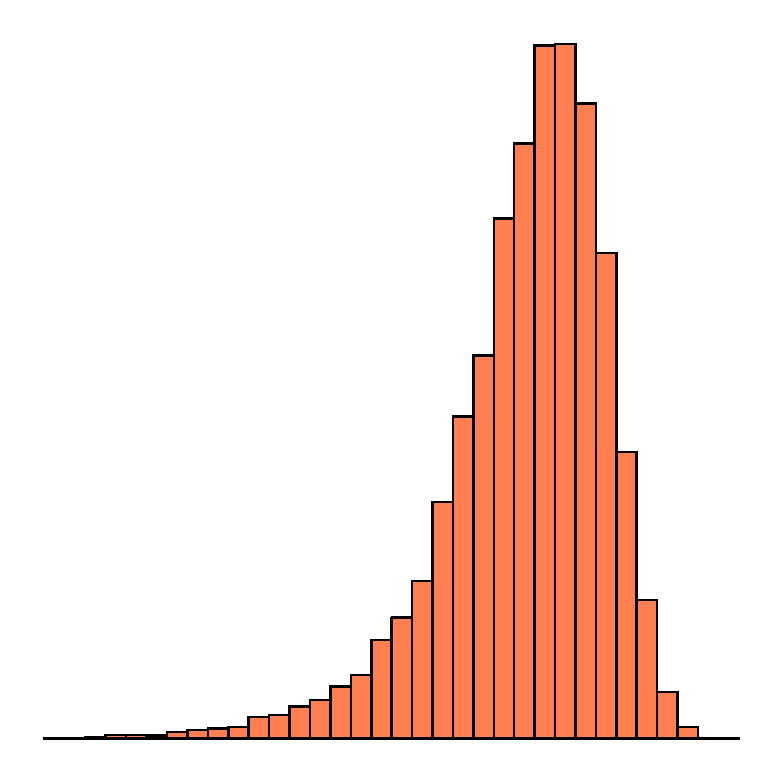
\includegraphics[scale=0.4]{img/descriptiva/histograma_asimetrico_izquierda.eps}}
% \psline[linewidth=15pt,linecolor=royalblue1,arrowlength=1,arrowinset=0]{->}(5,3)(7,3)
% \rput(6,3){$Y=X^2$}
% \rput[l](7,3){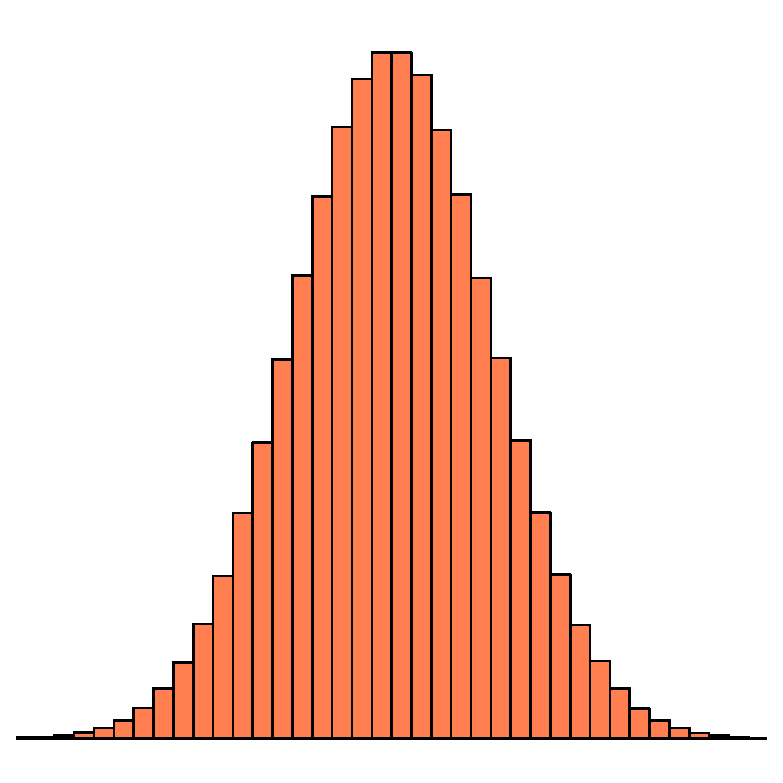
\includegraphics[scale=0.4]{img/descriptiva/histograma_simetrico.eps}}
% \end{pspicture}}
% \end{center}
% 
% \note{Otras transformaciones no lineales que son habituales para corregir anormalidades de la muestra son el cuadrado, que comprime la
% escala para valores pequeños y la expande para valores altos, de manera que es muy útil para corregir asimetrías hacia la izquierda, tal y
% como puede apreciarse en estos histogramas.
% }
% \end{frame}
% 
% 
% %---------------------------------------------------------------------slide----
% \begin{frame}
% \frametitle{Transformaciones no lineales}
% Las transformaciones $Y=\sqrt x$, $Y= \log X$ y $Y=1/X$ comprimen la escala para valores altos y la expanden para valores pequeños, de manera que son útiles para corregir asimetrías hacia la
% derecha.
% \begin{center}
% \scalebox{1}{
% \begin{pspicture}(0,0)(12,6)
% \rput[l](0,3){\reflectbox{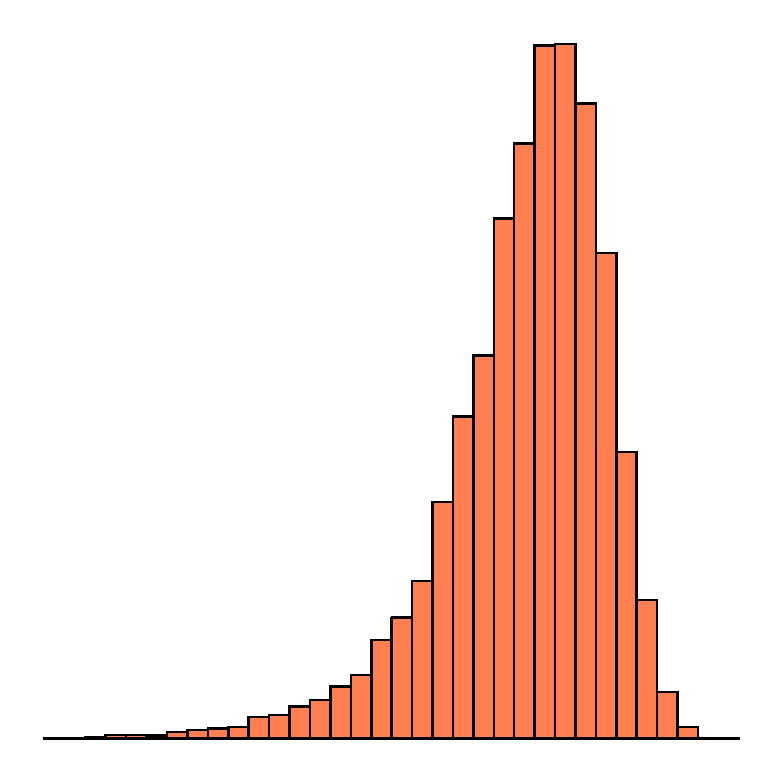
\includegraphics[scale=0.4]{img/descriptiva/histograma_asimetrico_izquierda.eps}}}
% \psline[linewidth=15pt,linecolor=royalblue1,arrowlength=1,arrowinset=0]{->}(5,3)(7,3)
% \rput(6,3){$Y=\sqrt{X}$}
% \rput[l](7,3){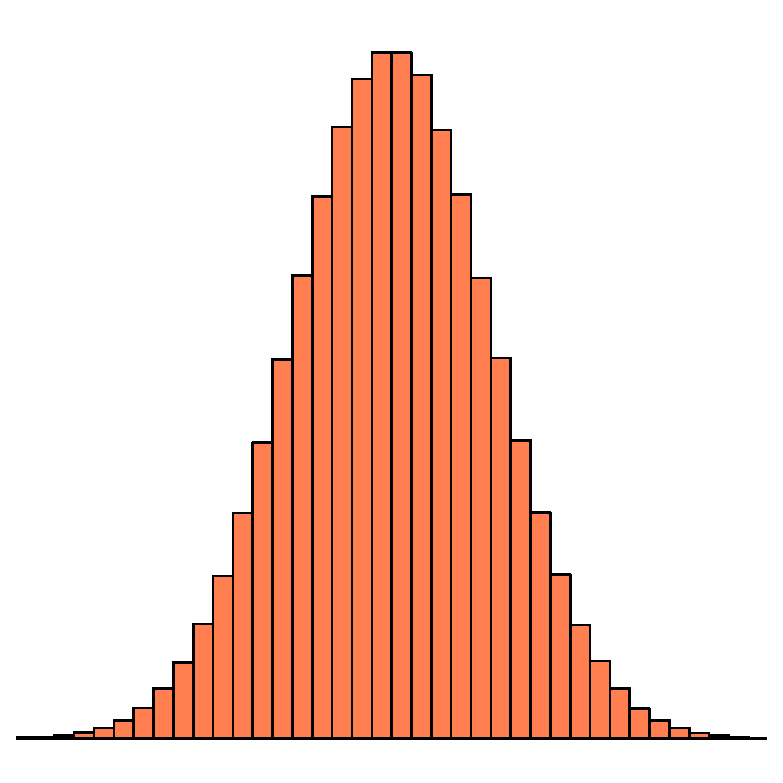
\includegraphics[scale=0.4]{img/descriptiva/histograma_simetrico.eps}}
% \end{pspicture}}
% \end{center}
% 
% \note{Mientras que para corregir asimetrías hacia la derecha se utilizan o bien la raíz cuadrada, la función logarítmica o la inversa, ya
% que ambas comprimen la escala para valores altos y la expanden para valores pequeños.}
% \end{frame}
% 
% 
% 
% %---------------------------------------------------------------------slide----
% \begin{frame}
% \frametitle{Variables clasificadoras o factores}
% En ocasiones interesa describir el comportamiento de una variable, no para toda la muestra, sino para distintos grupos de individuos, como por ejemplo, estudiar las estaturas en hombres y mujeres por separado. 
% 
% En tal caso se utiliza una nueva variable, llamada \highlight{\textbf{variable clasificadora}} o \highlight{\textbf{factor discriminante}}, para dividir la muestra en grupos y posteriormente se realiza el estudio descriptivo de la variable principal en cada grupo.
% \note{En ocasiones interesa describir el comportamiento de una variable, no para toda la muestra, sino para distintos grupos de individuos,
% como por ejemplo, estudiar las estaturas en hombres y mujeres por separado.
% 
% En tal caso se utiliza una nueva variable, llamada \highlight{\textbf{variable clasificadora}} o \highlight{\textbf{factor discriminante}},
% para dividir la muestra en grupos y posteriormente se realiza el estudio descriptivo de la variable principal en cada grupo. }
% \end{frame}
% 
% 
% %---------------------------------------------------------------------slide----
% \begin{frame}
% \frametitle{Variables clasificadoras}
% Usando la misma muestra de estaturas, pero teniendo en cuenta el sexo, tenemos:
% \begin{center}
% \begin{tabular}{lll}
% \hline
% \multirow{2}{*}{Mujeres} &
% 173, 158, 174, 166, 162, 177, 165, 154, 166, 182, \\
% & 169, 172, 170, 168. \\
% \hline
% \multirow{2}{*}{Hombres} &
% 179, 181, 172, 194, 185, 187, 198, 178, 188, 171,\\ 
% & 175, 167, 186, 172, 176, 187. \\
% \hline
% \end{tabular}
% \end{center}
% \begin{center}
% \scalebox{0.5}{%% Input file name: histograma_estatura_sexo.fig
%% FIG version: 3.2
%% Orientation: Landscape
%% Justification: Flush Left
%% Units: Inches
%% Paper size: A4
%% Magnification: 100.0
%% Resolution: 1200ppi

\begin{pspicture}(6.06cm,3.48cm)(16.82cm,13.45cm)
\psset{unit=0.8cm}
%%
%% Depth: 2147483647
%%
\newgray{mycolor0}{0.74}\definecolor{mycolor0}{gray}{0.74}
\newrgbcolor{mycolor1}{1.00 0.50 0.31}\definecolor{mycolor1}{rgb}{1.00,0.50,0.31}
\newrgbcolor{mycolor2}{0.28 0.46 1.00}\definecolor{mycolor2}{rgb}{0.28,0.46,1.00}
%%
%% Depth: 100
%%
\psset{linestyle=solid,linewidth=0.03175,linecolor=black,fillstyle=none}
\pspolygon(15.27,6.80)(15.27,8.43)(15.27,8.43)(15.27,6.80)(15.27,6.80)
\pspolygon(15.27,8.43)(15.27,10.06)(14.26,10.06)(14.26,8.43)(15.27,8.43)
\pspolygon(15.27,10.06)(15.27,11.69)(11.75,11.69)(11.75,10.06)(15.27,10.06)
\pspolygon(15.27,11.69)(15.27,13.32)(12.25,13.32)(12.25,11.69)(15.27,11.69)
\pspolygon(15.27,13.32)(15.27,14.95)(14.26,14.95)(14.26,13.32)(15.27,13.32)
\rput(15.27,15.99){\textbf{Histograma de estaturas por sexo}}
\psline(10.23,6.47)(20.31,6.47)
\psline(10.23,6.47)(10.23,6.30)
\psline(12.75,6.47)(12.75,6.30)
\psline(15.27,6.47)(15.27,6.30)
\psline(17.79,6.47)(17.79,6.30)
\psline(20.31,6.47)(20.31,6.30)
\rput(10.23,5.84){10}
\rput(12.75,5.84){5}
\rput(15.27,5.84){0}
\rput(17.79,5.84){5}
\rput(20.31,5.84){10}
\psline(10.23,6.80)(10.23,14.95)
\psline(10.23,6.80)(10.06,6.80)
\psline(10.23,8.43)(10.06,8.43)
\psline(10.23,10.06)(10.06,10.06)
\psline(10.23,11.69)(10.06,11.69)
\psline(10.23,13.32)(10.06,13.32)
\psline(10.23,14.95)(10.06,14.95)
\rput{90}(9.85,6.80){150.0}
\rput{90}(9.85,8.43){160.0}
\rput{90}(9.85,10.06){170.0}
\rput{90}(9.85,11.69){180.0}
\rput{90}(9.85,13.32){190.0}
\rput{90}(9.85,14.95){200.0}
\rput(13.18,4.86){Hombres}
\rput[r](18.17,4.86){Mujeres}
\rput{90}(8.88,10.88){Estatura}
\psline(15.27,6.47)(15.27,15.28)
\psline(10.23,6.47)(20.31,6.47)(20.31,15.28)(10.23,15.28)(10.23,6.47)
\psset{linestyle=dotted,linecolor=mycolor0}
\psline(10.23,6.47)(10.23,15.28)
\psline(11.24,6.47)(11.24,15.28)
\psline(12.25,6.47)(12.25,15.28)
\psline(13.26,6.47)(13.26,15.28)
\psline(14.26,6.47)(14.26,15.28)
\psline(15.27,6.47)(15.27,15.28)
\psline(16.28,6.47)(16.28,15.28)
\psline(17.29,6.47)(17.29,15.28)
\psline(18.29,6.47)(18.29,15.28)
\psline(19.30,6.47)(19.30,15.28)
\psset{linestyle=solid,linecolor=black,fillstyle=solid,fillcolor=mycolor1}
\pspolygon(15.27,6.80)(15.27,8.43)(15.27,8.43)(15.27,6.80)(15.27,6.80)
\pspolygon(15.27,8.43)(15.27,10.06)(14.26,10.06)(14.26,8.43)(15.27,8.43)
\pspolygon(15.27,10.06)(15.27,11.69)(11.75,11.69)(11.75,10.06)(15.27,10.06)
\pspolygon(15.27,11.69)(15.27,13.32)(12.25,13.32)(12.25,11.69)(15.27,11.69)
\pspolygon(15.27,13.32)(15.27,14.95)(14.26,14.95)(14.26,13.32)(15.27,13.32)
\psset{fillcolor=mycolor2}
\pspolygon(15.27,6.80)(15.27,8.43)(16.28,8.43)(16.28,6.80)(15.27,6.80)
\pspolygon(15.27,8.43)(15.27,10.06)(18.29,10.06)(18.29,8.43)(15.27,8.43)
\pspolygon(15.27,10.06)(15.27,11.69)(17.29,11.69)(17.29,10.06)(15.27,10.06)
\pspolygon(15.27,11.69)(15.27,13.32)(15.78,13.32)(15.78,11.69)(15.27,11.69)
\pspolygon(15.27,13.32)(15.27,14.95)(15.27,14.95)(15.27,13.32)(15.27,13.32)
\end{pspicture}
%% End
}
% \quad
% \scalebox{0.5}{%% Input file name: diagrama_cajas_estatura_sexo.fig
%% FIG version: 3.2
%% Orientation: Landscape
%% Justification: Flush Left
%% Units: Inches
%% Paper size: A4
%% Magnification: 100.0
%% Resolution: 1200ppi

\begin{pspicture}(6.06cm,3.48cm)(16.66cm,13.45cm)
\psset{unit=0.8cm}
%%
%% Depth: 2147483647
%%
\newrgbcolor{mycolor0}{1.00 0.50 0.31}\definecolor{mycolor0}{rgb}{1.00,0.50,0.31}
\newrgbcolor{mycolor1}{0.28 0.46 1.00}\definecolor{mycolor1}{rgb}{0.28,0.46,1.00}
%%
%% Depth: 100
%%
\psset{linestyle=solid,linewidth=0.0635,linecolor=black,fillstyle=none}
\psline(11.07,11.53)(14.81,11.53)
\psset{linestyle=dashed,linewidth=0.03175}
\psline(12.94,9.57)(12.94,10.39)
\psline(12.94,14.63)(12.94,12.83)
\psset{linestyle=solid}
\psline(12.01,9.57)(13.87,9.57)
\psline(12.01,14.63)(13.87,14.63)
\psline(11.07,10.39)(14.81,10.39)(14.81,12.83)(11.07,12.83)(11.07,10.39)
\psset{linewidth=0.0635}
\psline(15.74,9.73)(19.47,9.73)
\psset{linestyle=dashed,linewidth=0.03175}
\psline(17.60,7.45)(17.60,9.25)
\psline(17.60,12.02)(17.60,10.55)
\psset{linestyle=solid}
\psline(16.67,7.45)(18.54,7.45)
\psline(16.67,12.02)(18.54,12.02)
\psline(15.74,9.25)(19.47,9.25)(19.47,10.55)(15.74,10.55)(15.74,9.25)
\psline(12.94,6.47)(17.60,6.47)
\psline(12.94,6.47)(12.94,6.26)
\psline(17.60,6.47)(17.60,6.26)
\rput(12.94,5.71){hombre}
\rput(17.60,5.71){mujer}
\psline(10.23,6.80)(10.23,14.95)
\psline(10.23,6.80)(10.02,6.80)
\psline(10.23,8.43)(10.02,8.43)
\psline(10.23,10.06)(10.02,10.06)
\psline(10.23,11.69)(10.02,11.69)
\psline(10.23,13.32)(10.02,13.32)
\psline(10.23,14.95)(10.02,14.95)
\rput{90}(9.73,6.80){150}
\rput{90}(9.73,8.43){160}
\rput{90}(9.73,10.06){170}
\rput{90}(9.73,11.69){180}
\rput{90}(9.73,13.32){190}
\rput{90}(9.73,14.95){200}
\rput(15.27,15.99){\textbf{Diagrama de caja y bigotes de estaturas por sexo}}
\rput(15.27,4.86){Sexo}
\rput{90}(8.88,10.88){Estatura}
\psline(10.23,6.47)(20.31,6.47)(20.31,15.28)(10.23,15.28)(10.23,6.47)
\end{pspicture}
%% End
}
% \end{center}
% 
% \note{Si en el ejemplo de las estaturas hubiesemos tomado el sexo como factor, la muestra quedaría dividida en dos grupos, los hombres y
% las mujeres, y podríamos hacer un estudio descriptivo por separado de cada grupo para luego compararlos.}
% \end{frame}
% Autor: Alfredo Sánchez Alberca (asalber@ceu.es)

\section{Regresión y Correlación}

\mode<presentation>{
%---------------------------------------------------------------------slide----
\begin{frame}
\frametitle{Regresión y Correlación}
\tableofcontents[sectionstyle=show/hide,hideothersubsections]
\end{frame}
}


% ---------------------------------------------------------------------slide----
\begin{frame}
\frametitle{Relaciones entre variables}
Hasta ahora se ha visto como describir el comportamiento de una variable, pero en los fenómenos naturales normalmente aparecen más de una
variable que suelen estar relacionadas. 
Por ejemplo, en un estudio sobre el peso de las personas, deberíamos incluir todas las variables con las que podría tener relación: altura, edad, sexo, dieta, tabaco, ejercicio físico, etc.

Para comprender el fenómeno no basta con estudiar cada variable por separado y es preciso un estudio conjunto de todas las variables para ver cómo interactúan y qué relaciones se dan entre ellas. 
El objetivo de la estadística en este caso es dar medidas del grado y del tipo de relación
entre dichas variables.

Generalmente, en un \emph{estudio de dependencia} se considera una \highlight{variable dependiente} $Y$ que se supone relacionada con otras variables $X_1,\ldots,X_n$ llamadas
\highlight{variables independientes}.

El caso más simple es el de una sola variable independiente, y en tal caso se habla de \emph{estudio de dependencia simple}. Para más de una variable independiente se habla de \emph{estudio de dependencia múltiple}.

En este capítulo se verán los estudios de dependencia simple que son más sencillos.  

\note{En el tema anterior aprendimos a describir variables aisladas en una muestra, pero en la mayor parte de los fenómenos naturales
intervienen más de una variable que suelen estar relacionadas entre si, como por ejemplo en un estudio sobre el peso de las personas, habría
que incluir todas las variables con las que podría tener relación, como puede ser la altura, edad, sexo, dieta, tabaco, ejercicio físico,
etc.

Para comprender el fenómeno no basta con estudiar cada variable por separado y que hay que hacer un estudio conjunto de todas
las variables para ver cómo interactúan y qué relaciones se dan entre ellas. El objetivo de la estadística en este caso es dar medidas del
grado y del tipo de relación entre dichas variables.

En este tipo de estudios, generalmente se considera una \emph{variable dependiente} $Y$ que se supone relacionada con otras variables
$X_1,\ldots,X_n$ llamadas \emph{variables independientes}.

El caso más simple es el de una sola variable independiente, y en tal caso se habla de \emph{estudio de dependencia simple}. Para más de una
variable independiente se habla de \emph{estudio de dependencia múltiple}.

En este tema sólo se abordarán los estudios de dependencia simple que son los más sencillos, aunque muchos de los resultados pueden
generalizarse fácilmente a estudios de dependencia múltiple.}
\end{frame}


\subsection{Distribución de frecuencias conjunta}

% ---------------------------------------------------------------------slide----
\begin{frame}
\frametitle{Frecuencias conjuntas}
Al estudiar la dependencia simple entre dos variables $X$ e $Y$, no se pueden estudiar sus distribuciones por separado, sino que hay que estudiar la distribución conjunta de la \highlight{variable bidimensional} $(X,Y)$, cuyos valores son los pares $(x_i,y_j)$ donde el primer elemento es un valor $X$ y el segundo uno de $Y$.

\begin{definicion}[Frecuencias muestrales conjuntas]
Dada una muestra de tamaño $n$ de una variable bidimensional $(X,Y)$, para cada valor de la variable $(x_i,y_j)$ observado en la muestra se define:
\begin{itemize}
\item \structure{Frecuencia absoluta $n_{ij}$}: Es el número de veces que el par $(x_i,y_j)$ aparece en la muestra.
\item \structure{Frecuencia relativa $f_{ij}$}: Es la proporcion de veces que el par $(x_i,y_j)$ aparece en la muestra.
\[
f_{ij}=\frac{n_{ij}}{n}
\]
\end{itemize}
\end{definicion}
\begin{center}
\alert{\emph{¡Atención! Para las variables bidimensionales no tienen sentido las frecuencias acumuladas.}}
\end{center}
\note{Al igual que para las variables indivuales se definían las frecuencias muestrales, para las variables bidimensionales también se
pueden calcular frecuencias muestrales. En particular, para cada par de valores $(x_i,y_j)$ se puden calcular dos tipos de frecuencias, las
frecuenicas absolutas $n_{ij}$ que es el número de individuos de la muestra que presentan simultáneamente el valor $x_i$ de la variable $X$
y el valor $y_j$ de la variable $Y$, y la frecuencia relativa $f_{ij}$ que es el cociente de la frecuencia absoluta entre el tamaño de la
muestra y que por tanto da la proporción de individuos de la muestra que presentan simultáneamente el valor $x_i$ de la variable $X$ y el
valor $y_j$ de la variable $Y$. 

A diferencia de las variables individuales, para las variables bidimensionales no tiene sentido las frecuencias acumuladas ya que no se
pueden ordenar los pares con respecto a las dos variables a la vez.}
\end{frame}


%---------------------------------------------------------------------slide----
\begin{frame}
\frametitle{Distribución de frecuencias bidimensional}
Al conjunto de valores de la variable bidimensional y sus respectivas frecuencias muestrales se le denomina \structure{\textbf{distribución conjunta}}, y se representa mediante una \highlight{tabla de frecuencias bidimensional}.

\[
\begin{array}{|c|ccccc|}
\hline
X\backslash Y & y_1 & \cdots & y_j & \cdots & y_q\\
\hline
x_1 & n_{11} & \cdots & n_{1j} & \cdots & n_{1q}\\
\vdots & \vdots & \vdots & \vdots & \vdots & \vdots\\
x_i & n_{i1} & \cdots & n_{ij} & \cdots & n_{iq}\\
\vdots & \vdots & \vdots & \vdots & \vdots & \vdots\\
x_p & n_{p1} & \cdots & n_{pj} & \cdots & n_{pq}\\
\hline
\end{array}
\]

\note{Al conjunto de valores de la variable bidimensional y sus respectivas frecuencias muestrales se le denomina \structure{\textbf{distribución
conjunta}}.

La distribución conjunta de una variable bidimensional se suele representar mediante una \structure{\textbf{tabla de frecuencias
bidimensional}}.

\[
\begin{array}{|c|ccccc|}
\hline
X\backslash Y & y_1 & \cdots & y_j & \cdots & y_q\\
\hline
x_1 & n_{11} & \cdots & n_{1j} & \cdots & n_{1q}\\
\vdots & \vdots & \vdots & \vdots & \vdots & \vdots\\
x_i & n_{i1} & \cdots & n_{ij} & \cdots & n_{iq}\\
\vdots & \vdots & \vdots & \vdots & \vdots & \vdots\\
x_p & n_{p1} & \cdots & n_{pj} & \cdots & n_{pq}\\
\hline
\end{array}
\]
En esta tabla, se colocan los valores de una de las variables en la primera fila y los valores de la otra en la primera columna, y se
colocan las frecuencias absolutas o relativas correspondientes a cada par $(x_i,y_j)$ en la casilla correspondiente a la fila del valor
$x_i$ y la columna del valor $y_j$.}
\end{frame}


%---------------------------------------------------------------------slide----
\begin{frame}
\frametitle{Distribución de frecuencias bidimensional}
\framesubtitle{Ejemplo con estaturas y pesos}
La estatura (en cm) y el peso (en Kg) de una muestra de 30 estudiantes es:
\begin{center}
(179,85), (173,65), (181,71), (170,65), (158,51), (174,66), (172,62),\\ 
(166,60), (194,90), (185,75),(162,55), (187,78), (198,109), (177,61),\\ 
(178,70), (165,58), (154,50), (183,93),(166,51), (171,65), (175,70), \\
(182,60), (167,59), (169,62), (172,70), (186,71), (172,54), (176,68),\\
(168,67), (187,80).
\end{center}
La tabla de frecuencias bidimensional es
%\setlength\arraycolsep{3mm}
%\setlength\arrayrulewidth{0.5pt}
\[
\begin{array}{|c||c|c|c|c|c|c|}
\hline
  X/Y & [50,60) & [60,70) & [70,80) & [80,90) & [90,100) & [100,110) \\
  \hline\hline
  (150,160] & 2 & 0 & 0 & 0 & 0 & 0 \\
  \hline
  (160,170] & 4 & 4 & 0 & 0 & 0 & 0 \\
  \hline
  (170,180] & 1 & 6 & 3 & 1 & 0 & 0 \\
  \hline
  (180,190] & 0 & 1 & 4 & 1 & 1 & 0 \\
  \hline
  (190,200] & 0 & 0 & 0 & 0 & 1 & 1 \\
  \hline
\end{array}
\]

\note{En este ejemplo se han medido la Estatura y el Peso en una muestra de 30 estudiantes obteniendo estos datos. 
Para construir la tabla de frecuencias bidimensional, como ambas variables son continuas y tanto los valores de la estatura como los del
peso se repiten poco, conviene agrupar los datos de ambas variables en intervalos. Para la estatura construiremos 5 intervalos desde 150 a
200 cm y se colocan en la primera columna de la tabla. Para el peso construiremos 6 intervalos desde 50 a 110 kg y los colocaremos en la
primera fila de la tabla. Después procedemos a calcular las frecuenicas absolutas de cada par. Empezando por el primer par, su frecuencia
absoluta será el número de individuos en la muestra que miden entre 150 y 160 cm y pesan entre 50 y 60 kg. Mirando en la muestra se observa
que hay dos, $(158,51)$ y $(154,50)$, y por tanto la frecuencia absoluta de este par es 2. La frecuencia absoluta del par correspondiente
las estaturas entre 150 y 160 y peso entre 60 y 70 es 0 porque no hay nadie en la muestra con estatura entre 150 y 160 y peso entre 60 y 70.
De este modo se van calculando el resto de las frecuencias hasta completar la tabla.}
\end{frame}


%---------------------------------------------------------------------slide----
\begin{frame}
\frametitle{Diagrama de dispersión}
La distribución de frecuencias conjunta de una variable bidimensional puede representarse gráficamente mediante un \highlight{diagrama de dispersión}, donde los datos se representan como una colección de puntos en un plano cartesiano.

Habitualmente la variable independiente se representa en el eje $X$ y la variable dependiente en el eje $Y$.
Por cada par de valores $(x_i,y_j)$ en la muestra se dibuja un punto en el plano con esas coordenadas.
\begin{center}
\tikzsetnextfilename{regresion/diagrama_dispersion}
\resizebox{0.4\textwidth}{!}{% Author: Alfredo Sánchez Alberca (asalber@ceu.es)

\pgfplotsset{
    standard/.style={
        axis x line=bottom,
        axis y line=left,
        %enlarge x limits=-0.15,
        %enlarge y limits=-0.15,
        every axis x label/.style={at={(current axis.right of origin)},anchor=north west, font=\Large},
        every axis y label/.style={at={(current axis.above origin)},anchor=east, font=\Large},
    }
}

\begin{tikzpicture}
\begin{axis}[standard,ymin=0,ymax=5,axis
equal,xlabel={$X$},ylabel={$Y$},xtick={4},xticklabels={\Large $x_i$},ytick={3},yticklabels={\Large $y_j$}]
\addplot[color=color1,mark=*,domain=0:7] coordinates {(4,3)}; \coordinate (A) at (axis cs:4,3); \node[anchor=south west]
at (A) {\Large $(x_i,y_j)$}; \draw[dashed,color=gray] (axis cs:0,3) -- (A) -- (axis cs:4,0);
\end{axis}

\end{tikzpicture}}
\end{center}

El resultado es un conjunto de puntos que se conoce como \emph{nube de puntos}.

%En un diagrama de dispersión sólo se recogen los valores observados en la muestra, no las frecuencias de los mismos. Para reflejar las frecuencias tendríamos que recurrir a otro tipo de representación como un \emph{diagrama de burbujas} o \emph{histograma tridimensional}.

\begin{center}
\alert{\emph{¡Ojo! No tiene sentido cuando alguna de las variables es un atributo.}}
\end{center}
\note{La distribución de frecuencias bidimensional también suele representarse gráficamente y para ello se utiliza un diagrama conocido
como \structure{\textbf{diagrama de dispersión}} y que consiste en dibujar sobre un plano cartesiano los puntos que se corresponden con los
valores $(x_i,y_j)$ de la variable bidimensional, con lo que se obtiene una especie de nube de puntos cuya forma dependerá de la relación
entre las variables $X$ e $Y$. 

Hay que advertir que el diagrama de dispersión sólo refleja los valores observados en la muestra pero no las frecuencias de los mismos.
Además este diagrama sólo tiene sentido para variables cuantitativas y por tanto no puede dibujarse cuando alguna de las variables es un
atributo. }
\end{frame}


%---------------------------------------------------------------------slide----
\begin{frame}
\frametitle{Diagrama de dispersión}
\begin{center}
\tikzsetnextfilename{regresion/diagrama_dispersion_estatura_peso}
\mode<article>{\resizebox{0.7\textwidth}{!}{%% Input file name: diagrama_dispersion_estatura_peso.fig
%% FIG version: 3.2
%% Orientation: Landscape
%% Justification: Flush Left
%% Units: Inches
%% Paper size: A4
%% Magnification: 100.0
%% Resolution: 1200ppi
%% Include the following in the preamble:
%% \usepackage{textcomp}
%% End

\begin{pspicture}(5.94cm,3.48cm)(16.66cm,13.45cm)
\psset{unit=0.8cm}
%%
%% Depth: 2147483647
%%
\newrgbcolor{mycolor0}{1.00 0.50 0.31}\definecolor{mycolor0}{rgb}{1.00,0.50,0.31}
\newgray{mycolor1}{0.74}\definecolor{mycolor1}{gray}{0.74}
%%
%% Depth: 100
%%
\psset{linestyle=solid,linewidth=0.03175,linecolor=mycolor0}
\qdisk(16.02,11.64){0.1}
\qdisk(14.90,8.87){0.1}
\qdisk(16.39,9.70){0.1}
\qdisk(14.34,8.87){0.1}
\qdisk(12.10,6.94){0.1}
\qdisk(15.09,9.01){0.1}
\qdisk(14.71,8.46){0.1}
\qdisk(13.59,8.18){0.1}
\qdisk(18.82,12.33){0.1}
\qdisk(17.14,10.25){0.1}
\qdisk(12.85,7.49){0.1}
\qdisk(17.51,10.67){0.1}
\qdisk(19.56,14.95){0.1}
\qdisk(15.65,8.32){0.1}
\qdisk(15.83,9.56){0.1}
\qdisk(13.41,7.91){0.1}
\qdisk(11.35,6.80){0.1}
\qdisk(16.77,12.74){0.1}
\qdisk(13.59,6.94){0.1}
\qdisk(14.53,8.87){0.1}
\qdisk(15.27,9.56){0.1}
\qdisk(16.58,8.18){0.1}
\qdisk(13.78,8.04){0.1}
\qdisk(14.15,8.46){0.1}
\qdisk(14.71,9.56){0.1}
\qdisk(17.32,9.70){0.1}
\qdisk(14.71,7.35){0.1}
\qdisk(15.46,9.29){0.1}
\qdisk(13.97,9.15){0.1}
\qdisk(17.51,10.95){0.1}
\psset{linecolor=black,fillstyle=none}
\psline(10.61,6.47)(19.94,6.47)
\psline(10.61,6.47)(10.61,6.26)
\psline(12.47,6.47)(12.47,6.26)
\psline(14.34,6.47)(14.34,6.26)
\psline(16.21,6.47)(16.21,6.26)
\psline(18.07,6.47)(18.07,6.26)
\psline(19.94,6.47)(19.94,6.26)
\rput(10.61,5.71){150}
\rput(12.47,5.71){160}
\rput(14.34,5.71){170}
\rput(16.21,5.71){180}
\rput(18.07,5.71){190}
\rput(19.94,5.71){200}
\psline(10.23,6.80)(10.23,15.09)
\psline(10.23,6.80)(10.02,6.80)
\psline(10.23,8.18)(10.02,8.18)
\psline(10.23,9.56)(10.02,9.56)
\psline(10.23,10.95)(10.02,10.95)
\psline(10.23,12.33)(10.02,12.33)
\psline(10.23,13.71)(10.02,13.71)
\psline(10.23,15.09)(10.02,15.09)
\rput{90}(9.73,6.80){50}
\rput{90}(9.73,8.18){60}
\rput{90}(9.73,9.56){70}
\rput{90}(9.73,10.95){80}
\rput{90}(9.73,12.33){90}
\rput{90}(9.73,13.71){100}
\rput{90}(9.73,15.09){110}
\psline(10.23,6.47)(20.31,6.47)(20.31,15.28)(10.23,15.28)(10.23,6.47)
\rput(15.27,15.99){Diagrama de dispersión de Estaturas y Pesos}
\rput(15.27,4.86){Estatura (cm)}
\rput{90}(8.88,10.88){Peso (Kg)}
\psset{linestyle=dashed,linecolor=mycolor1}
\psline(16.02,6.47)(16.02,11.64)
\psline(10.23,11.64)(16.02,11.64)
\rput(16.02,12){$(179,85)$}
\end{pspicture}
%% End
}}
\mode<presentation>{\resizebox{0.9\textwidth}{!}{%% Input file name: diagrama_dispersion_estatura_peso.fig
%% FIG version: 3.2
%% Orientation: Landscape
%% Justification: Flush Left
%% Units: Inches
%% Paper size: A4
%% Magnification: 100.0
%% Resolution: 1200ppi
%% Include the following in the preamble:
%% \usepackage{textcomp}
%% End

\begin{pspicture}(5.94cm,3.48cm)(16.66cm,13.45cm)
\psset{unit=0.8cm}
%%
%% Depth: 2147483647
%%
\newrgbcolor{mycolor0}{1.00 0.50 0.31}\definecolor{mycolor0}{rgb}{1.00,0.50,0.31}
\newgray{mycolor1}{0.74}\definecolor{mycolor1}{gray}{0.74}
%%
%% Depth: 100
%%
\psset{linestyle=solid,linewidth=0.03175,linecolor=mycolor0}
\qdisk(16.02,11.64){0.1}
\qdisk(14.90,8.87){0.1}
\qdisk(16.39,9.70){0.1}
\qdisk(14.34,8.87){0.1}
\qdisk(12.10,6.94){0.1}
\qdisk(15.09,9.01){0.1}
\qdisk(14.71,8.46){0.1}
\qdisk(13.59,8.18){0.1}
\qdisk(18.82,12.33){0.1}
\qdisk(17.14,10.25){0.1}
\qdisk(12.85,7.49){0.1}
\qdisk(17.51,10.67){0.1}
\qdisk(19.56,14.95){0.1}
\qdisk(15.65,8.32){0.1}
\qdisk(15.83,9.56){0.1}
\qdisk(13.41,7.91){0.1}
\qdisk(11.35,6.80){0.1}
\qdisk(16.77,12.74){0.1}
\qdisk(13.59,6.94){0.1}
\qdisk(14.53,8.87){0.1}
\qdisk(15.27,9.56){0.1}
\qdisk(16.58,8.18){0.1}
\qdisk(13.78,8.04){0.1}
\qdisk(14.15,8.46){0.1}
\qdisk(14.71,9.56){0.1}
\qdisk(17.32,9.70){0.1}
\qdisk(14.71,7.35){0.1}
\qdisk(15.46,9.29){0.1}
\qdisk(13.97,9.15){0.1}
\qdisk(17.51,10.95){0.1}
\psset{linecolor=black,fillstyle=none}
\psline(10.61,6.47)(19.94,6.47)
\psline(10.61,6.47)(10.61,6.26)
\psline(12.47,6.47)(12.47,6.26)
\psline(14.34,6.47)(14.34,6.26)
\psline(16.21,6.47)(16.21,6.26)
\psline(18.07,6.47)(18.07,6.26)
\psline(19.94,6.47)(19.94,6.26)
\rput(10.61,5.71){150}
\rput(12.47,5.71){160}
\rput(14.34,5.71){170}
\rput(16.21,5.71){180}
\rput(18.07,5.71){190}
\rput(19.94,5.71){200}
\psline(10.23,6.80)(10.23,15.09)
\psline(10.23,6.80)(10.02,6.80)
\psline(10.23,8.18)(10.02,8.18)
\psline(10.23,9.56)(10.02,9.56)
\psline(10.23,10.95)(10.02,10.95)
\psline(10.23,12.33)(10.02,12.33)
\psline(10.23,13.71)(10.02,13.71)
\psline(10.23,15.09)(10.02,15.09)
\rput{90}(9.73,6.80){50}
\rput{90}(9.73,8.18){60}
\rput{90}(9.73,9.56){70}
\rput{90}(9.73,10.95){80}
\rput{90}(9.73,12.33){90}
\rput{90}(9.73,13.71){100}
\rput{90}(9.73,15.09){110}
\psline(10.23,6.47)(20.31,6.47)(20.31,15.28)(10.23,15.28)(10.23,6.47)
\rput(15.27,15.99){Diagrama de dispersión de Estaturas y Pesos}
\rput(15.27,4.86){Estatura (cm)}
\rput{90}(8.88,10.88){Peso (Kg)}
\psset{linestyle=dashed,linecolor=mycolor1}
\psline(16.02,6.47)(16.02,11.64)
\psline(10.23,11.64)(16.02,11.64)
\rput(16.02,12){$(179,85)$}
\end{pspicture}
%% End
}}
\end{center}
\note{En este ejemplo se muestra el diagrama de dispersión correspondiente al ejemplo de las estasturas y los pesos de los 30 estudiantes.
Cada punto de la nube de puntos corresponde a un individuo de la muestra. Así, por ejemplo, este punto, con coordenada $X$ 179 y coordenada
$Y$ 85 corresponde al primer individuo de la muestra que medía 179 cm y pesaba 85 kg.}
\end{frame}


%---------------------------------------------------------------------slide----
\begin{frame}
\frametitle{Interpretación del diagrama de dispersión}
El diagrama de dispersión da información visual sobre el tipo de relación entre las variables.

\tikzsetnextfilename{regresion/diagrama_dispersion_tipos_relaciones}
\resizebox{\textwidth}{!}{% Created by tikzDevice version 0.10.1 on 2016-02-27 12:38:36
% !TEX encoding = UTF-8 Unicode
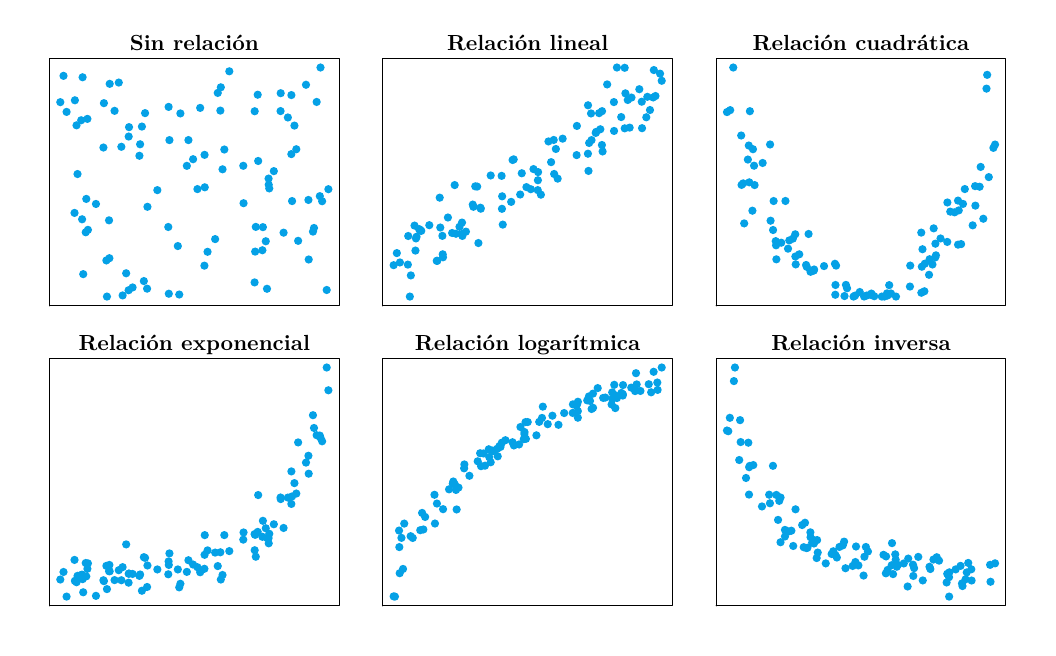
\begin{tikzpicture}[x=1pt,y=1pt]
\definecolor{fillColor}{RGB}{255,255,255}
\path[use as bounding box,fill=fillColor,fill opacity=0.00] (0,0) rectangle (361.35,216.81);
\begin{scope}
\path[clip] (  7.92,116.33) rectangle (112.53,205.72);
\definecolor{fillColor}{RGB}{5,161,230}

\path[fill=fillColor] (100.57,196.18) circle (  1.49);

\path[fill=fillColor] ( 63.92,170.85) circle (  1.49);

\path[fill=fillColor] ( 67.74,140.41) circle (  1.49);

\path[fill=fillColor] ( 43.15,122.50) circle (  1.49);

\path[fill=fillColor] ( 72.86,201.04) circle (  1.49);

\path[fill=fillColor] ( 92.47,142.73) circle (  1.49);

\path[fill=fillColor] ( 29.40,147.19) circle (  1.49);

\path[fill=fillColor] ( 55.18,185.82) circle (  1.49);

\path[fill=fillColor] ( 95.28,171.12) circle (  1.49);

\path[fill=fillColor] ( 27.55,189.53) circle (  1.49);

\path[fill=fillColor] (106.40,154.10) circle (  1.49);

\path[fill=fillColor] ( 94.02,184.36) circle (  1.49);

\path[fill=fillColor] ( 78.01,153.38) circle (  1.49);

\path[fill=fillColor] ( 71.06,172.78) circle (  1.49);

\path[fill=fillColor] ( 34.31,120.06) circle (  1.49);

\path[fill=fillColor] ( 42.42,185.93) circle (  1.49);

\path[fill=fillColor] ( 31.40,186.76) circle (  1.49);

\path[fill=fillColor] ( 41.28,181.07) circle (  1.49);

\path[fill=fillColor] ( 50.81,144.79) circle (  1.49);

\path[fill=fillColor] ( 43.28,152.08) circle (  1.49);

\path[fill=fillColor] ( 68.69,193.23) circle (  1.49);

\path[fill=fillColor] ( 91.38,186.67) circle (  1.49);

\path[fill=fillColor] ( 88.95,164.97) circle (  1.49);

\path[fill=fillColor] ( 87.05,162.28) circle (  1.49);

\path[fill=fillColor] ( 40.63,174.67) circle (  1.49);

\path[fill=fillColor] ( 40.38,170.52) circle (  1.49);

\path[fill=fillColor] (103.46,144.43) circle (  1.49);

\path[fill=fillColor] (104.42,189.97) circle (  1.49);

\path[fill=fillColor] ( 50.93,188.18) circle (  1.49);

\path[fill=fillColor] ( 82.03,186.61) circle (  1.49);

\path[fill=fillColor] (108.06,122.02) circle (  1.49);

\path[fill=fillColor] ( 46.86,158.10) circle (  1.49);

\path[fill=fillColor] ( 77.91,166.90) circle (  1.49);

\path[fill=fillColor] ( 62.33,187.82) circle (  1.49);

\path[fill=fillColor] ( 69.79,195.26) circle (  1.49);

\path[fill=fillColor] ( 97.73,139.78) circle (  1.49);

\path[fill=fillColor] ( 85.00,144.73) circle (  1.49);

\path[fill=fillColor] ( 17.65,181.52) circle (  1.49);

\path[fill=fillColor] (105.81,202.41) circle (  1.49);

\path[fill=fillColor] ( 82.00,124.76) circle (  1.49);

\path[fill=fillColor] ( 35.59,128.06) circle (  1.49);

\path[fill=fillColor] ( 17.06,190.57) circle (  1.49);

\path[fill=fillColor] ( 82.20,135.89) circle (  1.49);

\path[fill=fillColor] ( 86.48,122.46) circle (  1.49);

\path[fill=fillColor] ( 83.29,168.64) circle (  1.49);

\path[fill=fillColor] ( 32.92,196.97) circle (  1.49);

\path[fill=fillColor] ( 87.10,160.06) circle (  1.49);

\path[fill=fillColor] ( 14.06,186.37) circle (  1.49);

\path[fill=fillColor] ( 33.85,173.77) circle (  1.49);

\path[fill=fillColor] ( 69.63,186.84) circle (  1.49);

\path[fill=fillColor] ( 96.39,181.42) circle (  1.49);

\path[fill=fillColor] ( 63.86,130.81) circle (  1.49);

\path[fill=fillColor] ( 57.52,166.88) circle (  1.49);

\path[fill=fillColor] ( 24.68,153.11) circle (  1.49);

\path[fill=fillColor] ( 63.99,159.13) circle (  1.49);

\path[fill=fillColor] ( 12.95,199.40) circle (  1.49);

\path[fill=fillColor] ( 19.85,198.89) circle (  1.49);

\path[fill=fillColor] ( 61.34,158.48) circle (  1.49);

\path[fill=fillColor] ( 28.65,119.64) circle (  1.49);

\path[fill=fillColor] ( 16.93,149.87) circle (  1.49);

\path[fill=fillColor] ( 51.22,176.18) circle (  1.49);

\path[fill=fillColor] ( 37.91,122.94) circle (  1.49);

\path[fill=fillColor] ( 36.46,121.93) circle (  1.49);

\path[fill=fillColor] ( 54.77,120.38) circle (  1.49);

\path[fill=fillColor] (105.57,155.93) circle (  1.49);

\path[fill=fillColor] ( 29.64,196.51) circle (  1.49);

\path[fill=fillColor] ( 65.00,135.82) circle (  1.49);

\path[fill=fillColor] ( 51.00,120.67) circle (  1.49);

\path[fill=fillColor] (108.66,158.44) circle (  1.49);

\path[fill=fillColor] ( 21.18,154.93) circle (  1.49);

\path[fill=fillColor] ( 58.09,176.19) circle (  1.49);

\path[fill=fillColor] ( 20.07,127.75) circle (  1.49);

\path[fill=fillColor] ( 28.44,132.70) circle (  1.49);

\path[fill=fillColor] ( 95.29,192.45) circle (  1.49);

\path[fill=fillColor] ( 27.37,173.50) circle (  1.49);

\path[fill=fillColor] ( 18.01,163.92) circle (  1.49);

\path[fill=fillColor] ( 11.79,189.89) circle (  1.49);

\path[fill=fillColor] ( 20.98,142.88) circle (  1.49);

\path[fill=fillColor] ( 21.58,183.85) circle (  1.49);

\path[fill=fillColor] ( 29.53,133.51) circle (  1.49);

\path[fill=fillColor] ( 70.41,165.63) circle (  1.49);

\path[fill=fillColor] ( 59.77,169.28) circle (  1.49);

\path[fill=fillColor] ( 19.34,183.35) circle (  1.49);

\path[fill=fillColor] ( 82.43,144.82) circle (  1.49);

\path[fill=fillColor] ( 41.98,125.24) circle (  1.49);

\path[fill=fillColor] ( 86.04,139.63) circle (  1.49);

\path[fill=fillColor] (103.09,143.11) circle (  1.49);

\path[fill=fillColor] ( 83.12,192.58) circle (  1.49);

\path[fill=fillColor] ( 87.30,158.72) circle (  1.49);

\path[fill=fillColor] ( 21.77,143.75) circle (  1.49);

\path[fill=fillColor] (101.45,154.56) circle (  1.49);

\path[fill=fillColor] ( 95.54,154.15) circle (  1.49);

\path[fill=fillColor] ( 36.50,177.47) circle (  1.49);

\path[fill=fillColor] ( 91.43,193.13) circle (  1.49);

\path[fill=fillColor] ( 84.81,136.38) circle (  1.49);

\path[fill=fillColor] ( 36.63,180.87) circle (  1.49);

\path[fill=fillColor] (101.55,133.04) circle (  1.49);

\path[fill=fillColor] ( 97.07,172.88) circle (  1.49);

\path[fill=fillColor] ( 54.26,137.90) circle (  1.49);

\path[fill=fillColor] ( 19.67,147.57) circle (  1.49);
\end{scope}
\begin{scope}
\path[clip] (  0.00,108.41) rectangle (120.45,216.81);
\definecolor{drawColor}{RGB}{0,0,0}

\node[text=drawColor,anchor=base,inner sep=0pt, outer sep=0pt, scale=  0.79] at ( 60.22,208.50) {\bfseries Sin relación};

\node[text=drawColor,anchor=base,inner sep=0pt, outer sep=0pt, scale=  0.66] at ( 60.22, 86.23) {$X$};
\end{scope}
\begin{scope}
\path[clip] (  0.00,  0.00) rectangle (361.35,216.81);
\definecolor{drawColor}{RGB}{0,0,0}

\path[draw=drawColor,line width= 0.4pt,line join=round,line cap=round] (  7.92,116.33) --
	(112.53,116.33) --
	(112.53,205.72) --
	(  7.92,205.72) --
	(  7.92,116.33);
\end{scope}
\begin{scope}
\path[clip] (128.37,116.33) rectangle (232.98,205.72);
\definecolor{fillColor}{RGB}{5,161,230}

\path[fill=fillColor] (221.02,194.57) circle (  1.49);

\path[fill=fillColor] (184.37,161.67) circle (  1.49);

\path[fill=fillColor] (188.19,175.70) circle (  1.49);

\path[fill=fillColor] (163.60,151.76) circle (  1.49);

\path[fill=fillColor] (193.31,176.70) circle (  1.49);

\path[fill=fillColor] (212.92,202.41) circle (  1.49);

\path[fill=fillColor] (149.85,141.58) circle (  1.49);

\path[fill=fillColor] (175.63,169.22) circle (  1.49);

\path[fill=fillColor] (215.73,202.31) circle (  1.49);

\path[fill=fillColor] (148.00,132.56) circle (  1.49);

\path[fill=fillColor] (226.85,192.11) circle (  1.49);

\path[fill=fillColor] (214.47,184.51) circle (  1.49);

\path[fill=fillColor] (198.46,181.30) circle (  1.49);

\path[fill=fillColor] (191.51,162.26) circle (  1.49);

\path[fill=fillColor] (154.76,142.34) circle (  1.49);

\path[fill=fillColor] (162.87,138.99) circle (  1.49);

\path[fill=fillColor] (151.85,148.21) circle (  1.49);

\path[fill=fillColor] (161.73,159.47) circle (  1.49);

\path[fill=fillColor] (171.26,163.26) circle (  1.49);

\path[fill=fillColor] (163.73,151.39) circle (  1.49);

\path[fill=fillColor] (189.14,168.22) circle (  1.49);

\path[fill=fillColor] (211.83,189.92) circle (  1.49);

\path[fill=fillColor] (209.40,196.30) circle (  1.49);

\path[fill=fillColor] (207.50,174.41) circle (  1.49);

\path[fill=fillColor] (161.08,152.08) circle (  1.49);

\path[fill=fillColor] (160.83,152.88) circle (  1.49);

\path[fill=fillColor] (223.91,191.82) circle (  1.49);

\path[fill=fillColor] (224.87,187.05) circle (  1.49);

\path[fill=fillColor] (171.38,151.35) circle (  1.49);

\path[fill=fillColor] (202.48,188.77) circle (  1.49);

\path[fill=fillColor] (228.51,200.19) circle (  1.49);

\path[fill=fillColor] (167.31,163.40) circle (  1.49);

\path[fill=fillColor] (198.36,170.76) circle (  1.49);

\path[fill=fillColor] (182.78,165.71) circle (  1.49);

\path[fill=fillColor] (190.24,163.94) circle (  1.49);

\path[fill=fillColor] (218.18,191.55) circle (  1.49);

\path[fill=fillColor] (205.45,179.17) circle (  1.49);

\path[fill=fillColor] (138.10,119.64) circle (  1.49);

\path[fill=fillColor] (226.26,201.49) circle (  1.49);

\path[fill=fillColor] (202.45,171.26) circle (  1.49);

\path[fill=fillColor] (156.04,144.86) circle (  1.49);

\path[fill=fillColor] (137.51,141.53) circle (  1.49);

\path[fill=fillColor] (202.65,165.05) circle (  1.49);

\path[fill=fillColor] (206.93,180.10) circle (  1.49);

\path[fill=fillColor] (203.74,176.17) circle (  1.49);

\path[fill=fillColor] (153.37,142.62) circle (  1.49);

\path[fill=fillColor] (207.55,186.64) circle (  1.49);

\path[fill=fillColor] (134.51,131.97) circle (  1.49);

\path[fill=fillColor] (154.30,159.93) circle (  1.49);

\path[fill=fillColor] (190.08,176.23) circle (  1.49);

\path[fill=fillColor] (216.84,190.68) circle (  1.49);

\path[fill=fillColor] (184.31,158.11) circle (  1.49);

\path[fill=fillColor] (177.97,156.52) circle (  1.49);

\path[fill=fillColor] (145.13,145.44) circle (  1.49);

\path[fill=fillColor] (184.44,164.62) circle (  1.49);

\path[fill=fillColor] (133.40,135.35) circle (  1.49);

\path[fill=fillColor] (140.30,140.66) circle (  1.49);

\path[fill=fillColor] (181.79,158.44) circle (  1.49);

\path[fill=fillColor] (149.10,144.59) circle (  1.49);

\path[fill=fillColor] (137.38,131.19) circle (  1.49);

\path[fill=fillColor] (171.67,145.64) circle (  1.49);

\path[fill=fillColor] (158.36,143.10) circle (  1.49);

\path[fill=fillColor] (156.91,142.27) circle (  1.49);

\path[fill=fillColor] (175.22,169.00) circle (  1.49);

\path[fill=fillColor] (226.02,191.60) circle (  1.49);

\path[fill=fillColor] (150.09,133.85) circle (  1.49);

\path[fill=fillColor] (185.45,156.46) circle (  1.49);

\path[fill=fillColor] (171.45,155.87) circle (  1.49);

\path[fill=fillColor] (229.11,197.62) circle (  1.49);

\path[fill=fillColor] (141.63,143.87) circle (  1.49);

\path[fill=fillColor] (178.54,164.20) circle (  1.49);

\path[fill=fillColor] (140.52,141.26) circle (  1.49);

\path[fill=fillColor] (148.89,155.38) circle (  1.49);

\path[fill=fillColor] (215.74,180.43) circle (  1.49);

\path[fill=fillColor] (147.82,132.55) circle (  1.49);

\path[fill=fillColor] (138.46,127.29) circle (  1.49);

\path[fill=fillColor] (132.24,130.99) circle (  1.49);

\path[fill=fillColor] (141.43,144.00) circle (  1.49);

\path[fill=fillColor] (142.03,143.48) circle (  1.49);

\path[fill=fillColor] (149.98,134.92) circle (  1.49);

\path[fill=fillColor] (190.86,172.98) circle (  1.49);

\path[fill=fillColor] (180.22,159.20) circle (  1.49);

\path[fill=fillColor] (139.79,145.29) circle (  1.49);

\path[fill=fillColor] (202.88,175.15) circle (  1.49);

\path[fill=fillColor] (162.43,159.39) circle (  1.49);

\path[fill=fillColor] (206.49,185.92) circle (  1.49);

\path[fill=fillColor] (223.54,184.43) circle (  1.49);

\path[fill=fillColor] (203.57,185.81) circle (  1.49);

\path[fill=fillColor] (207.75,172.08) circle (  1.49);

\path[fill=fillColor] (142.22,143.38) circle (  1.49);

\path[fill=fillColor] (221.90,190.05) circle (  1.49);

\path[fill=fillColor] (215.99,193.08) circle (  1.49);

\path[fill=fillColor] (156.95,146.38) circle (  1.49);

\path[fill=fillColor] (211.88,179.49) circle (  1.49);

\path[fill=fillColor] (205.26,178.78) circle (  1.49);

\path[fill=fillColor] (157.08,141.56) circle (  1.49);

\path[fill=fillColor] (222.00,180.49) circle (  1.49);

\path[fill=fillColor] (217.52,180.69) circle (  1.49);

\path[fill=fillColor] (174.71,153.86) circle (  1.49);

\path[fill=fillColor] (140.12,136.26) circle (  1.49);
\end{scope}
\begin{scope}
\path[clip] (120.45,108.41) rectangle (240.90,216.81);
\definecolor{drawColor}{RGB}{0,0,0}

\node[text=drawColor,anchor=base,inner sep=0pt, outer sep=0pt, scale=  0.79] at (180.68,208.50) {\bfseries Relación lineal};

\node[text=drawColor,anchor=base,inner sep=0pt, outer sep=0pt, scale=  0.66] at (180.68, 86.23) {$X$};

\node[text=drawColor,rotate= 90.00,anchor=base,inner sep=0pt, outer sep=0pt, scale=  0.66] at (103.03,161.02) {$Y$};
\end{scope}
\begin{scope}
\path[clip] (  0.00,  0.00) rectangle (361.35,216.81);
\definecolor{drawColor}{RGB}{0,0,0}

\path[draw=drawColor,line width= 0.4pt,line join=round,line cap=round] (128.37,116.33) --
	(232.98,116.33) --
	(232.98,205.72) --
	(128.37,205.72) --
	(128.37,116.33);
\end{scope}
\begin{scope}
\path[clip] (248.82,116.33) rectangle (353.43,205.72);
\definecolor{fillColor}{RGB}{5,161,230}

\path[fill=fillColor] (341.47,145.38) circle (  1.49);

\path[fill=fillColor] (304.82,120.43) circle (  1.49);

\path[fill=fillColor] (308.64,119.64) circle (  1.49);

\path[fill=fillColor] (284.05,129.03) circle (  1.49);

\path[fill=fillColor] (313.76,119.64) circle (  1.49);

\path[fill=fillColor] (333.37,150.33) circle (  1.49);

\path[fill=fillColor] (270.30,139.67) circle (  1.49);

\path[fill=fillColor] (296.08,122.65) circle (  1.49);

\path[fill=fillColor] (336.18,154.32) circle (  1.49);

\path[fill=fillColor] (268.45,147.06) circle (  1.49);

\path[fill=fillColor] (347.30,162.81) circle (  1.49);

\path[fill=fillColor] (334.92,150.08) circle (  1.49);

\path[fill=fillColor] (318.91,130.83) circle (  1.49);

\path[fill=fillColor] (311.96,120.75) circle (  1.49);

\path[fill=fillColor] (275.21,139.94) circle (  1.49);

\path[fill=fillColor] (283.32,128.85) circle (  1.49);

\path[fill=fillColor] (272.30,139.11) circle (  1.49);

\path[fill=fillColor] (282.18,142.26) circle (  1.49);

\path[fill=fillColor] (291.71,131.49) circle (  1.49);

\path[fill=fillColor] (284.18,129.42) circle (  1.49);

\path[fill=fillColor] (309.59,119.65) circle (  1.49);

\path[fill=fillColor] (332.28,139.39) circle (  1.49);

\path[fill=fillColor] (329.85,140.64) circle (  1.49);

\path[fill=fillColor] (327.95,133.78) circle (  1.49);

\path[fill=fillColor] (281.53,130.38) circle (  1.49);

\path[fill=fillColor] (281.28,131.05) circle (  1.49);

\path[fill=fillColor] (344.36,166.49) circle (  1.49);

\path[fill=fillColor] (345.32,147.77) circle (  1.49);

\path[fill=fillColor] (291.83,120.30) circle (  1.49);

\path[fill=fillColor] (322.93,121.02) circle (  1.49);

\path[fill=fillColor] (348.96,173.38) circle (  1.49);

\path[fill=fillColor] (287.76,130.66) circle (  1.49);

\path[fill=fillColor] (318.81,123.26) circle (  1.49);

\path[fill=fillColor] (303.23,120.03) circle (  1.49);

\path[fill=fillColor] (310.69,120.02) circle (  1.49);

\path[fill=fillColor] (338.63,158.49) circle (  1.49);

\path[fill=fillColor] (325.90,133.14) circle (  1.49);

\path[fill=fillColor] (258.55,160.55) circle (  1.49);

\path[fill=fillColor] (346.71,199.76) circle (  1.49);

\path[fill=fillColor] (322.90,142.75) circle (  1.49);

\path[fill=fillColor] (276.49,140.57) circle (  1.49);

\path[fill=fillColor] (257.96,159.99) circle (  1.49);

\path[fill=fillColor] (323.10,130.43) circle (  1.49);

\path[fill=fillColor] (327.38,144.29) circle (  1.49);

\path[fill=fillColor] (324.19,131.53) circle (  1.49);

\path[fill=fillColor] (273.82,154.19) circle (  1.49);

\path[fill=fillColor] (328.00,138.75) circle (  1.49);

\path[fill=fillColor] (254.96,202.41) circle (  1.49);

\path[fill=fillColor] (274.75,136.95) circle (  1.49);

\path[fill=fillColor] (310.53,120.80) circle (  1.49);

\path[fill=fillColor] (337.29,138.60) circle (  1.49);

\path[fill=fillColor] (304.76,120.24) circle (  1.49);

\path[fill=fillColor] (298.42,119.64) circle (  1.49);

\path[fill=fillColor] (265.58,167.92) circle (  1.49);

\path[fill=fillColor] (304.89,120.72) circle (  1.49);

\path[fill=fillColor] (253.85,187.01) circle (  1.49);

\path[fill=fillColor] (260.75,160.92) circle (  1.49);

\path[fill=fillColor] (302.24,119.66) circle (  1.49);

\path[fill=fillColor] (269.55,154.17) circle (  1.49);

\path[fill=fillColor] (257.83,177.84) circle (  1.49);

\path[fill=fillColor] (292.12,130.83) circle (  1.49);

\path[fill=fillColor] (278.81,134.91) circle (  1.49);

\path[fill=fillColor] (277.36,142.15) circle (  1.49);

\path[fill=fillColor] (295.67,123.86) circle (  1.49);

\path[fill=fillColor] (346.47,194.78) circle (  1.49);

\path[fill=fillColor] (270.54,133.10) circle (  1.49);

\path[fill=fillColor] (305.90,119.77) circle (  1.49);

\path[fill=fillColor] (291.90,123.83) circle (  1.49);

\path[fill=fillColor] (349.56,174.57) circle (  1.49);

\path[fill=fillColor] (262.08,172.89) circle (  1.49);

\path[fill=fillColor] (298.99,119.99) circle (  1.49);

\path[fill=fillColor] (260.97,186.63) circle (  1.49);

\path[fill=fillColor] (269.34,143.69) circle (  1.49);

\path[fill=fillColor] (336.19,138.40) circle (  1.49);

\path[fill=fillColor] (268.27,174.60) circle (  1.49);

\path[fill=fillColor] (258.91,146.08) circle (  1.49);

\path[fill=fillColor] (252.69,186.31) circle (  1.49);

\path[fill=fillColor] (261.88,150.67) circle (  1.49);

\path[fill=fillColor] (262.48,166.93) circle (  1.49);

\path[fill=fillColor] (270.43,138.17) circle (  1.49);

\path[fill=fillColor] (311.31,123.77) circle (  1.49);

\path[fill=fillColor] (300.67,121.29) circle (  1.49);

\path[fill=fillColor] (260.24,169.15) circle (  1.49);

\path[fill=fillColor] (323.33,136.75) circle (  1.49);

\path[fill=fillColor] (282.88,128.60) circle (  1.49);

\path[fill=fillColor] (326.94,131.24) circle (  1.49);

\path[fill=fillColor] (343.99,159.33) circle (  1.49);

\path[fill=fillColor] (324.02,121.56) circle (  1.49);

\path[fill=fillColor] (328.20,134.54) circle (  1.49);

\path[fill=fillColor] (262.67,159.93) circle (  1.49);

\path[fill=fillColor] (342.35,159.55) circle (  1.49);

\path[fill=fillColor] (336.44,150.78) circle (  1.49);

\path[fill=fillColor] (277.40,134.12) circle (  1.49);

\path[fill=fillColor] (332.33,153.64) circle (  1.49);

\path[fill=fillColor] (325.71,127.51) circle (  1.49);

\path[fill=fillColor] (277.53,131.27) circle (  1.49);

\path[fill=fillColor] (342.45,152.50) circle (  1.49);

\path[fill=fillColor] (337.97,153.12) circle (  1.49);

\path[fill=fillColor] (295.16,119.83) circle (  1.49);

\path[fill=fillColor] (260.57,174.22) circle (  1.49);
\end{scope}
\begin{scope}
\path[clip] (240.90,108.41) rectangle (361.35,216.81);
\definecolor{drawColor}{RGB}{0,0,0}

\node[text=drawColor,anchor=base,inner sep=0pt, outer sep=0pt, scale=  0.79] at (301.12,208.50) {\bfseries Relación cuadrática};

\node[text=drawColor,anchor=base,inner sep=0pt, outer sep=0pt, scale=  0.66] at (301.12, 86.23) {$X$};

\node[text=drawColor,rotate= 90.00,anchor=base,inner sep=0pt, outer sep=0pt, scale=  0.66] at (223.48,161.02) {$Y$};
\end{scope}
\begin{scope}
\path[clip] (  0.00,  0.00) rectangle (361.35,216.81);
\definecolor{drawColor}{RGB}{0,0,0}

\path[draw=drawColor,line width= 0.4pt,line join=round,line cap=round] (248.82,116.33) --
	(353.43,116.33) --
	(353.43,205.72) --
	(248.82,205.72) --
	(248.82,116.33);
\end{scope}
\begin{scope}
\path[clip] (  7.92,  7.92) rectangle (112.53, 97.32);
\definecolor{fillColor}{RGB}{5,161,230}

\path[fill=fillColor] (100.57, 59.65) circle (  1.49);

\path[fill=fillColor] ( 63.92, 26.33) circle (  1.49);

\path[fill=fillColor] ( 67.74, 27.13) circle (  1.49);

\path[fill=fillColor] ( 43.15, 14.70) circle (  1.49);

\path[fill=fillColor] ( 72.86, 27.67) circle (  1.49);

\path[fill=fillColor] ( 92.47, 36.03) circle (  1.49);

\path[fill=fillColor] ( 29.40, 20.42) circle (  1.49);

\path[fill=fillColor] ( 55.18, 15.87) circle (  1.49);

\path[fill=fillColor] ( 95.28, 44.72) circle (  1.49);

\path[fill=fillColor] ( 27.55, 16.81) circle (  1.49);

\path[fill=fillColor] (106.40, 67.35) circle (  1.49);

\path[fill=fillColor] ( 94.02, 47.01) circle (  1.49);

\path[fill=fillColor] ( 78.01, 34.41) circle (  1.49);

\path[fill=fillColor] ( 71.06, 33.45) circle (  1.49);

\path[fill=fillColor] ( 34.31, 21.87) circle (  1.49);

\path[fill=fillColor] ( 42.42, 25.23) circle (  1.49);

\path[fill=fillColor] ( 31.40, 17.19) circle (  1.49);

\path[fill=fillColor] ( 41.28, 13.34) circle (  1.49);

\path[fill=fillColor] ( 50.81, 19.29) circle (  1.49);

\path[fill=fillColor] ( 43.28, 22.47) circle (  1.49);

\path[fill=fillColor] ( 68.69, 22.26) circle (  1.49);

\path[fill=fillColor] ( 91.38, 47.04) circle (  1.49);

\path[fill=fillColor] ( 88.95, 37.37) circle (  1.49);

\path[fill=fillColor] ( 87.05, 32.35) circle (  1.49);

\path[fill=fillColor] ( 40.63, 19.22) circle (  1.49);

\path[fill=fillColor] ( 40.38, 18.72) circle (  1.49);

\path[fill=fillColor] (103.46, 72.16) circle (  1.49);

\path[fill=fillColor] (104.42, 69.55) circle (  1.49);

\path[fill=fillColor] ( 50.93, 23.95) circle (  1.49);

\path[fill=fillColor] ( 82.03, 27.98) circle (  1.49);

\path[fill=fillColor] (108.06, 94.01) circle (  1.49);

\path[fill=fillColor] ( 46.86, 21.04) circle (  1.49);

\path[fill=fillColor] ( 77.91, 31.81) circle (  1.49);

\path[fill=fillColor] ( 62.33, 20.03) circle (  1.49);

\path[fill=fillColor] ( 69.79, 17.40) circle (  1.49);

\path[fill=fillColor] ( 97.73, 66.94) circle (  1.49);

\path[fill=fillColor] ( 85.00, 38.61) circle (  1.49);

\path[fill=fillColor] ( 17.65, 16.42) circle (  1.49);

\path[fill=fillColor] (105.81, 68.63) circle (  1.49);

\path[fill=fillColor] ( 82.00, 33.81) circle (  1.49);

\path[fill=fillColor] ( 35.59, 30.09) circle (  1.49);

\path[fill=fillColor] ( 17.06, 16.91) circle (  1.49);

\path[fill=fillColor] ( 82.20, 33.54) circle (  1.49);

\path[fill=fillColor] ( 86.48, 32.40) circle (  1.49);

\path[fill=fillColor] ( 83.29, 47.92) circle (  1.49);

\path[fill=fillColor] ( 32.92, 20.77) circle (  1.49);

\path[fill=fillColor] ( 87.10, 30.48) circle (  1.49);

\path[fill=fillColor] ( 14.06, 11.23) circle (  1.49);

\path[fill=fillColor] ( 33.85, 17.14) circle (  1.49);

\path[fill=fillColor] ( 69.63, 27.24) circle (  1.49);

\path[fill=fillColor] ( 96.39, 52.23) circle (  1.49);

\path[fill=fillColor] ( 63.86, 21.28) circle (  1.49);

\path[fill=fillColor] ( 57.52, 20.16) circle (  1.49);

\path[fill=fillColor] ( 24.68, 11.50) circle (  1.49);

\path[fill=fillColor] ( 63.99, 33.44) circle (  1.49);

\path[fill=fillColor] ( 12.95, 20.12) circle (  1.49);

\path[fill=fillColor] ( 19.85, 17.53) circle (  1.49);

\path[fill=fillColor] ( 61.34, 21.85) circle (  1.49);

\path[fill=fillColor] ( 28.65, 13.94) circle (  1.49);

\path[fill=fillColor] ( 16.93, 24.48) circle (  1.49);

\path[fill=fillColor] ( 51.22, 26.84) circle (  1.49);

\path[fill=fillColor] ( 37.91, 19.41) circle (  1.49);

\path[fill=fillColor] ( 36.46, 16.26) circle (  1.49);

\path[fill=fillColor] ( 54.77, 14.57) circle (  1.49);

\path[fill=fillColor] (105.57, 69.41) circle (  1.49);

\path[fill=fillColor] ( 29.64, 20.37) circle (  1.49);

\path[fill=fillColor] ( 65.00, 27.93) circle (  1.49);

\path[fill=fillColor] ( 51.00, 22.67) circle (  1.49);

\path[fill=fillColor] (108.66, 85.78) circle (  1.49);

\path[fill=fillColor] ( 21.18, 18.54) circle (  1.49);

\path[fill=fillColor] ( 58.09, 24.37) circle (  1.49);

\path[fill=fillColor] ( 20.07, 12.79) circle (  1.49);

\path[fill=fillColor] ( 28.44, 22.34) circle (  1.49);

\path[fill=fillColor] ( 95.29, 56.47) circle (  1.49);

\path[fill=fillColor] ( 27.37, 17.14) circle (  1.49);

\path[fill=fillColor] ( 18.01, 18.72) circle (  1.49);

\path[fill=fillColor] ( 11.79, 17.40) circle (  1.49);

\path[fill=fillColor] ( 20.98, 23.36) circle (  1.49);

\path[fill=fillColor] ( 21.58, 21.27) circle (  1.49);

\path[fill=fillColor] ( 29.53, 22.67) circle (  1.49);

\path[fill=fillColor] ( 70.41, 19.04) circle (  1.49);

\path[fill=fillColor] ( 59.77, 22.81) circle (  1.49);

\path[fill=fillColor] ( 19.34, 19.04) circle (  1.49);

\path[fill=fillColor] ( 82.43, 25.64) circle (  1.49);

\path[fill=fillColor] ( 41.98, 25.47) circle (  1.49);

\path[fill=fillColor] ( 86.04, 35.93) circle (  1.49);

\path[fill=fillColor] (103.09, 76.78) circle (  1.49);

\path[fill=fillColor] ( 83.12, 34.61) circle (  1.49);

\path[fill=fillColor] ( 87.30, 33.92) circle (  1.49);

\path[fill=fillColor] ( 21.77, 23.24) circle (  1.49);

\path[fill=fillColor] (101.45, 62.12) circle (  1.49);

\path[fill=fillColor] ( 95.54, 47.43) circle (  1.49);

\path[fill=fillColor] ( 36.50, 19.48) circle (  1.49);

\path[fill=fillColor] ( 91.43, 46.47) circle (  1.49);

\path[fill=fillColor] ( 84.81, 32.84) circle (  1.49);

\path[fill=fillColor] ( 36.63, 19.56) circle (  1.49);

\path[fill=fillColor] (101.55, 55.64) circle (  1.49);

\path[fill=fillColor] ( 97.07, 48.47) circle (  1.49);

\path[fill=fillColor] ( 54.26, 21.04) circle (  1.49);

\path[fill=fillColor] ( 19.67, 19.15) circle (  1.49);
\end{scope}
\begin{scope}
\path[clip] (  0.00,  0.00) rectangle (120.45,108.41);
\definecolor{drawColor}{RGB}{0,0,0}

\node[text=drawColor,anchor=base,inner sep=0pt, outer sep=0pt, scale=  0.79] at ( 60.22,100.09) {\bfseries Relación exponencial};
\end{scope}
\begin{scope}
\path[clip] (  0.00,  0.00) rectangle (361.35,216.81);
\definecolor{drawColor}{RGB}{0,0,0}

\path[draw=drawColor,line width= 0.4pt,line join=round,line cap=round] (  7.92,  7.92) --
	(112.53,  7.92) --
	(112.53, 97.32) --
	(  7.92, 97.32) --
	(  7.92,  7.92);
\end{scope}
\begin{scope}
\path[clip] (128.37,  7.92) rectangle (232.98, 97.32);
\definecolor{fillColor}{RGB}{5,161,230}

\path[fill=fillColor] (166.79, 61.64) circle (  1.49);

\path[fill=fillColor] (153.61, 52.04) circle (  1.49);

\path[fill=fillColor] (227.52, 88.58) circle (  1.49);

\path[fill=fillColor] (225.29, 85.05) circle (  1.49);

\path[fill=fillColor] (143.62, 40.01) circle (  1.49);

\path[fill=fillColor] (185.85, 75.79) circle (  1.49);

\path[fill=fillColor] (134.43, 19.68) circle (  1.49);

\path[fill=fillColor] (211.21, 85.02) circle (  1.49);

\path[fill=fillColor] (179.53, 70.69) circle (  1.49);

\path[fill=fillColor] (211.25, 82.67) circle (  1.49);

\path[fill=fillColor] (164.70, 62.95) circle (  1.49);

\path[fill=fillColor] (179.89, 74.28) circle (  1.49);

\path[fill=fillColor] (154.36, 51.77) circle (  1.49);

\path[fill=fillColor] (218.09, 86.74) circle (  1.49);

\path[fill=fillColor] (153.80, 52.82) circle (  1.49);

\path[fill=fillColor] (142.98, 35.48) circle (  1.49);

\path[fill=fillColor] (229.11, 94.01) circle (  1.49);

\path[fill=fillColor] (165.26, 58.54) circle (  1.49);

\path[fill=fillColor] (135.63, 21.22) circle (  1.49);

\path[fill=fillColor] (202.20, 82.14) circle (  1.49);

\path[fill=fillColor] (196.95, 77.59) circle (  1.49);

\path[fill=fillColor] (207.96, 83.03) circle (  1.49);

\path[fill=fillColor] (175.19, 67.01) circle (  1.49);

\path[fill=fillColor] (220.06, 87.91) circle (  1.49);

\path[fill=fillColor] (205.98, 86.57) circle (  1.49);

\path[fill=fillColor] (179.25, 68.12) circle (  1.49);

\path[fill=fillColor] (147.89, 44.85) circle (  1.49);

\path[fill=fillColor] (134.30, 29.12) circle (  1.49);

\path[fill=fillColor] (135.06, 32.45) circle (  1.49);

\path[fill=fillColor] (170.86, 65.32) circle (  1.49);

\path[fill=fillColor] (134.20, 35.09) circle (  1.49);

\path[fill=fillColor] (178.06, 72.51) circle (  1.49);

\path[fill=fillColor] (187.92, 73.54) circle (  1.49);

\path[fill=fillColor] (159.62, 54.88) circle (  1.49);

\path[fill=fillColor] (147.17, 37.63) circle (  1.49);

\path[fill=fillColor] (168.04, 63.99) circle (  1.49);

\path[fill=fillColor] (191.80, 73.30) circle (  1.49);

\path[fill=fillColor] (162.62, 60.12) circle (  1.49);

\path[fill=fillColor] (203.20, 81.93) circle (  1.49);

\path[fill=fillColor] (193.86, 77.55) circle (  1.49);

\path[fill=fillColor] (215.07, 84.37) circle (  1.49);

\path[fill=fillColor] (198.83, 81.64) circle (  1.49);

\path[fill=fillColor] (186.15, 79.87) circle (  1.49);

\path[fill=fillColor] (139.14, 32.42) circle (  1.49);

\path[fill=fillColor] (183.83, 69.50) circle (  1.49);

\path[fill=fillColor] (177.58, 66.21) circle (  1.49);

\path[fill=fillColor] (180.04, 68.23) circle (  1.49);

\path[fill=fillColor] (157.71, 57.58) circle (  1.49);

\path[fill=fillColor] (198.80, 75.87) circle (  1.49);

\path[fill=fillColor] (175.69, 65.85) circle (  1.49);

\path[fill=fillColor] (226.19, 92.46) circle (  1.49);

\path[fill=fillColor] (203.78, 79.02) circle (  1.49);

\path[fill=fillColor] (180.69, 74.30) circle (  1.49);

\path[fill=fillColor] (198.81, 78.26) circle (  1.49);

\path[fill=fillColor] (147.00, 48.02) circle (  1.49);

\path[fill=fillColor] (138.38, 33.06) circle (  1.49);

\path[fill=fillColor] (211.00, 80.67) circle (  1.49);

\path[fill=fillColor] (179.48, 69.99) circle (  1.49);

\path[fill=fillColor] (197.02, 80.69) circle (  1.49);

\path[fill=fillColor] (169.64, 64.62) circle (  1.49);

\path[fill=fillColor] (154.77, 49.77) circle (  1.49);

\path[fill=fillColor] (214.53, 84.80) circle (  1.49);

\path[fill=fillColor] (198.52, 80.75) circle (  1.49);

\path[fill=fillColor] (202.80, 83.57) circle (  1.49);

\path[fill=fillColor] (212.34, 79.34) circle (  1.49);

\path[fill=fillColor] (204.30, 79.44) circle (  1.49);

\path[fill=fillColor] (212.07, 84.09) circle (  1.49);

\path[fill=fillColor] (141.86, 35.22) circle (  1.49);

\path[fill=fillColor] (167.31, 59.77) circle (  1.49);

\path[fill=fillColor] (163.50, 63.03) circle (  1.49);

\path[fill=fillColor] (142.52, 41.46) circle (  1.49);

\path[fill=fillColor] (189.61, 76.60) circle (  1.49);

\path[fill=fillColor] (163.82, 58.36) circle (  1.49);

\path[fill=fillColor] (211.96, 87.76) circle (  1.49);

\path[fill=fillColor] (227.63, 85.92) circle (  1.49);

\path[fill=fillColor] (132.71, 11.23) circle (  1.49);

\path[fill=fillColor] (221.42, 85.54) circle (  1.49);

\path[fill=fillColor] (198.30, 80.24) circle (  1.49);

\path[fill=fillColor] (219.82, 91.96) circle (  1.49);

\path[fill=fillColor] (224.42, 87.97) circle (  1.49);

\path[fill=fillColor] (168.29, 63.80) circle (  1.49);

\path[fill=fillColor] (157.80, 58.99) circle (  1.49);

\path[fill=fillColor] (219.48, 85.49) circle (  1.49);

\path[fill=fillColor] (136.07, 37.61) circle (  1.49);

\path[fill=fillColor] (155.68, 50.62) circle (  1.49);

\path[fill=fillColor] (132.24, 11.31) circle (  1.49);

\path[fill=fillColor] (208.73, 83.14) circle (  1.49);

\path[fill=fillColor] (150.10, 42.82) circle (  1.49);

\path[fill=fillColor] (170.45, 65.55) circle (  1.49);

\path[fill=fillColor] (184.84, 74.37) circle (  1.49);

\path[fill=fillColor] (215.13, 87.66) circle (  1.49);

\path[fill=fillColor] (172.64, 67.74) circle (  1.49);

\path[fill=fillColor] (166.61, 64.47) circle (  1.49);

\path[fill=fillColor] (155.01, 42.71) circle (  1.49);

\path[fill=fillColor] (171.33, 66.84) circle (  1.49);

\path[fill=fillColor] (215.02, 83.87) circle (  1.49);

\path[fill=fillColor] (169.86, 61.92) circle (  1.49);

\path[fill=fillColor] (212.94, 82.98) circle (  1.49);

\path[fill=fillColor] (204.26, 84.57) circle (  1.49);

\path[fill=fillColor] (152.27, 49.99) circle (  1.49);
\end{scope}
\begin{scope}
\path[clip] (120.45,  0.00) rectangle (240.90,108.41);
\definecolor{drawColor}{RGB}{0,0,0}

\node[text=drawColor,anchor=base,inner sep=0pt, outer sep=0pt, scale=  0.79] at (180.68,100.09) {\bfseries Relación logarítmica};

\node[text=drawColor,rotate= 90.00,anchor=base,inner sep=0pt, outer sep=0pt, scale=  0.66] at (103.03, 52.62) {$Y$};
\end{scope}
\begin{scope}
\path[clip] (  0.00,  0.00) rectangle (361.35,216.81);
\definecolor{drawColor}{RGB}{0,0,0}

\path[draw=drawColor,line width= 0.4pt,line join=round,line cap=round] (128.37,  7.92) --
	(232.98,  7.92) --
	(232.98, 97.32) --
	(128.37, 97.32) --
	(128.37,  7.92);
\end{scope}
\begin{scope}
\path[clip] (248.82,  7.92) rectangle (353.43, 97.32);
\definecolor{fillColor}{RGB}{5,161,230}

\path[fill=fillColor] (288.38, 23.23) circle (  1.49);

\path[fill=fillColor] (260.41, 66.84) circle (  1.49);

\path[fill=fillColor] (327.30, 24.62) circle (  1.49);

\path[fill=fillColor] (340.98, 21.10) circle (  1.49);

\path[fill=fillColor] (312.22, 22.57) circle (  1.49);

\path[fill=fillColor] (284.12, 30.42) circle (  1.49);

\path[fill=fillColor] (294.54, 29.74) circle (  1.49);

\path[fill=fillColor] (291.10, 27.61) circle (  1.49);

\path[fill=fillColor] (323.44, 17.07) circle (  1.49);

\path[fill=fillColor] (332.93, 18.25) circle (  1.49);

\path[fill=fillColor] (271.57, 45.81) circle (  1.49);

\path[fill=fillColor] (291.86, 26.29) circle (  1.49);

\path[fill=fillColor] (282.83, 34.45) circle (  1.49);

\path[fill=fillColor] (313.50, 26.49) circle (  1.49);

\path[fill=fillColor] (283.45, 30.70) circle (  1.49);

\path[fill=fillColor] (310.74, 20.87) circle (  1.49);

\path[fill=fillColor] (298.11, 22.30) circle (  1.49);

\path[fill=fillColor] (302.36, 25.63) circle (  1.49);

\path[fill=fillColor] (299.09, 23.72) circle (  1.49);

\path[fill=fillColor] (255.19, 89.10) circle (  1.49);

\path[fill=fillColor] (252.69, 71.24) circle (  1.49);

\path[fill=fillColor] (312.33, 30.55) circle (  1.49);

\path[fill=fillColor] (270.54, 47.97) circle (  1.49);

\path[fill=fillColor] (332.28, 19.46) circle (  1.49);

\path[fill=fillColor] (318.19, 24.96) circle (  1.49);

\path[fill=fillColor] (337.09, 22.33) circle (  1.49);

\path[fill=fillColor] (337.80, 15.04) circle (  1.49);

\path[fill=fillColor] (326.18, 21.20) circle (  1.49);

\path[fill=fillColor] (281.76, 28.87) circle (  1.49);

\path[fill=fillColor] (253.16, 70.99) circle (  1.49);

\path[fill=fillColor] (260.70, 57.99) circle (  1.49);

\path[fill=fillColor] (285.26, 31.65) circle (  1.49);

\path[fill=fillColor] (317.97, 14.88) circle (  1.49);

\path[fill=fillColor] (314.06, 22.02) circle (  1.49);

\path[fill=fillColor] (273.64, 32.95) circle (  1.49);

\path[fill=fillColor] (269.31, 58.48) circle (  1.49);

\path[fill=fillColor] (257.43, 74.99) circle (  1.49);

\path[fill=fillColor] (290.51, 26.63) circle (  1.49);

\path[fill=fillColor] (260.65, 48.09) circle (  1.49);

\path[fill=fillColor] (329.32, 24.22) circle (  1.49);

\path[fill=fillColor] (274.94, 34.76) circle (  1.49);

\path[fill=fillColor] (332.97, 11.23) circle (  1.49);

\path[fill=fillColor] (320.02, 18.69) circle (  1.49);

\path[fill=fillColor] (265.34, 43.80) circle (  1.49);

\path[fill=fillColor] (295.52, 21.48) circle (  1.49);

\path[fill=fillColor] (333.05, 20.00) circle (  1.49);

\path[fill=fillColor] (349.56, 23.25) circle (  1.49);

\path[fill=fillColor] (276.63, 29.52) circle (  1.49);

\path[fill=fillColor] (257.12, 60.58) circle (  1.49);

\path[fill=fillColor] (335.32, 21.06) circle (  1.49);

\path[fill=fillColor] (295.02, 31.09) circle (  1.49);

\path[fill=fillColor] (316.58, 23.21) circle (  1.49);

\path[fill=fillColor] (285.49, 27.14) circle (  1.49);

\path[fill=fillColor] (268.22, 44.95) circle (  1.49);

\path[fill=fillColor] (302.05, 18.83) circle (  1.49);

\path[fill=fillColor] (262.19, 58.76) circle (  1.49);

\path[fill=fillColor] (284.07, 31.62) circle (  1.49);

\path[fill=fillColor] (253.73, 75.83) circle (  1.49);

\path[fill=fillColor] (325.87, 22.01) circle (  1.49);

\path[fill=fillColor] (281.38, 28.76) circle (  1.49);

\path[fill=fillColor] (292.39, 25.35) circle (  1.49);

\path[fill=fillColor] (347.92, 16.59) circle (  1.49);

\path[fill=fillColor] (321.82, 25.58) circle (  1.49);

\path[fill=fillColor] (277.46, 42.77) circle (  1.49);

\path[fill=fillColor] (312.70, 19.35) circle (  1.49);

\path[fill=fillColor] (267.93, 48.05) circle (  1.49);

\path[fill=fillColor] (280.89, 37.91) circle (  1.49);

\path[fill=fillColor] (280.42, 29.08) circle (  1.49);

\path[fill=fillColor] (260.92, 58.46) circle (  1.49);

\path[fill=fillColor] (313.66, 24.53) circle (  1.49);

\path[fill=fillColor] (271.15, 38.94) circle (  1.49);

\path[fill=fillColor] (320.31, 21.52) circle (  1.49);

\path[fill=fillColor] (300.18, 22.50) circle (  1.49);

\path[fill=fillColor] (332.06, 16.33) circle (  1.49);

\path[fill=fillColor] (310.18, 25.75) circle (  1.49);

\path[fill=fillColor] (285.10, 25.16) circle (  1.49);

\path[fill=fillColor] (341.09, 17.04) circle (  1.49);

\path[fill=fillColor] (328.49, 25.46) circle (  1.49);

\path[fill=fillColor] (337.62, 15.98) circle (  1.49);

\path[fill=fillColor] (339.33, 19.98) circle (  1.49);

\path[fill=fillColor] (339.87, 23.39) circle (  1.49);

\path[fill=fillColor] (310.10, 19.64) circle (  1.49);

\path[fill=fillColor] (299.32, 29.33) circle (  1.49);

\path[fill=fillColor] (257.64, 67.07) circle (  1.49);

\path[fill=fillColor] (279.86, 37.09) circle (  1.49);

\path[fill=fillColor] (255.57, 94.01) circle (  1.49);

\path[fill=fillColor] (272.04, 30.87) circle (  1.49);

\path[fill=fillColor] (293.33, 29.17) circle (  1.49);

\path[fill=fillColor] (302.89, 29.16) circle (  1.49);

\path[fill=fillColor] (314.47, 22.68) circle (  1.49);

\path[fill=fillColor] (275.96, 35.04) circle (  1.49);

\path[fill=fillColor] (338.89, 17.47) circle (  1.49);

\path[fill=fillColor] (272.05, 47.04) circle (  1.49);

\path[fill=fillColor] (319.90, 22.76) circle (  1.49);

\path[fill=fillColor] (347.77, 22.70) circle (  1.49);

\path[fill=fillColor] (259.57, 54.09) circle (  1.49);

\path[fill=fillColor] (303.63, 27.52) circle (  1.49);

\path[fill=fillColor] (273.64, 35.33) circle (  1.49);

\path[fill=fillColor] (282.89, 32.69) circle (  1.49);

\path[fill=fillColor] (309.25, 26.32) circle (  1.49);
\end{scope}
\begin{scope}
\path[clip] (240.90,  0.00) rectangle (361.35,108.41);
\definecolor{drawColor}{RGB}{0,0,0}

\node[text=drawColor,anchor=base,inner sep=0pt, outer sep=0pt, scale=  0.79] at (301.12,100.09) {\bfseries Relación inversa};

\node[text=drawColor,rotate= 90.00,anchor=base,inner sep=0pt, outer sep=0pt, scale=  0.66] at (223.48, 52.62) {$Y$};
\end{scope}
\begin{scope}
\path[clip] (  0.00,  0.00) rectangle (361.35,216.81);
\definecolor{drawColor}{RGB}{0,0,0}

\path[draw=drawColor,line width= 0.4pt,line join=round,line cap=round] (248.82,  7.92) --
	(353.43,  7.92) --
	(353.43, 97.32) --
	(248.82, 97.32) --
	(248.82,  7.92);
\end{scope}
\end{tikzpicture}
}

\note{Dependiendo del tipo de relación entre las variables, la nube de puntos del diagrama de dispersión tendrá distintas formas. Aquí se
presentan algunos ejemplos.

En el primer caso tenemos un diagrama de dispersión de dos variables independientes. En este caso la nube de
puntos no tendrá una forma definida aunque normalmentes los puntos formarán un cúmulo circular.

En el segundo caso tenemos el diagrama de dispersión de dos variables relacionadas linealmente. En este caso la nube de puntos tendrá una
forma más o menos de recta.

En el tercer caso tenemos el diagrama de dispersión de dos variables relacionadas parabólicamente, de forma que la nube de puntos tiene
forma de parábola.

El cuarto caso se corresponde con una relación exponencial, donde la nube de puntos tiene más o menos la forma de una curva exponencial.

El quinto caso corresponde a una relación logarítmica, donde la nube de puntos tiene forma de curva logarítmica.

Y finalmente el último caso correspondería a una relación inversa.}
\end{frame}


%---------------------------------------------------------------------slide----
\begin{frame}
\frametitle{Distribuciones marginales}
A cada una de las distribuciones de las variables que conforman la variable bidimensional se les llama \structure{\textbf{distribuciones marginales}}.

Las distribuciones marginales se pueden obtener a partir de la tabla de frecuencias bidimensional, sumando las frecuencias por filas y columnas.
\begin{center}
\[
\begin{array}{|c|ccccc|>{\columncolor{color1!50}}c|}
\hline
X\backslash Y & y_1 & \cdots & y_j & \cdots & y_q & n_x\\
\hline
x_1 & n_{11} & \cdots & n_{1j} & \cdots & n_{1q} & n_{x_1}\\
\vdots & \vdots & \vdots & \tikz[baseline=-0.5ex]{\node at (0,0) [fill=color2!50,single arrow,shape border
rotate=270, single arrow head extend=1mm]{$+$\phantom{}}; } & \vdots &
\vdots & \vdots \\
x_i & n_{i1} & \tikz[baseline=-0.5ex]{\node at (0,0) [fill=color1!50,single arrow,shape border rotate=0,
single arrow head extend=1mm]{$+$\phantom{}}; }  & n_{ij} & \tikz[baseline=-0.5ex]{\node
at (0,0) [fill=color1!50,single arrow,shape border rotate=0, single
arrow head extend=1mm]{$+$\phantom{}}; } & n_{iq} & n_{x_i}\\
\vdots & \vdots & \vdots & \tikz[baseline=-0.5ex]{\node at (0,0) [fill=color2!50,single arrow,shape border
rotate=270, single arrow head extend=1mm]{$+$\phantom{}}; } & \vdots & \vdots & \vdots\\
x_p & n_{p1} & \cdots & n_{pj} & \cdots & n_{pq} & n_{x_p} \\
\hline
\rowcolor{color2!50}
n_y & n_{y_1} & \cdots & n_{y_j} & \cdots & n_{y_q} & \cellcolor{white} n\\
\hline
\end{array}
\]
\end{center}

\note{A partir de la tabla de frecuencias bidimensional es posible obtener la distribución de frecuencias de cada una de las variables
individuales que componen la variable bidimensional sumando las frecuencias de la tabla por filas para una de las variables y por columnas
para otra. Por ejemplo, para obtener la frecuencia absoluta de $x_i$ basta sumar las frecuencias absolutas que aparecen en la fila
correspondiente a $x_i$, mientras que para obtener la frecuencia de $y_i$ hay que sumar las frecuencias absolutas que aparecen en la
columna correspondiente a $y_j$. 

Como las distribuciones de cada variable aparecen en los márgenes de la tabla, se les llama distribuciones
marginales.}
\end{frame}


%---------------------------------------------------------------------slide----
\begin{frame}
\frametitle{Distribuciones marginales}
\framesubtitle{Ejemplo con estaturas y pesos}
En el ejemplo anterior de las estaturas y los pesos, las distribuciones marginales son
\[
\begin{array}{|c||c|c|c|c|c|c|>{\columncolor{color1!50}}c|}
\hline
  X/Y & [50,60) & [60,70) & [70,80) & [80,90) & [90,100) & [100,110) & n_x\\
  \hline\hline
  (150,160] & 2 & 0 & 0 & 0 & 0 & 0 & 2\\
  \hline
  (160,170] & 4 & 4 & 0 & 0 & 0 & 0 & 8\\
  \hline
  (170,180] & 1 & 6 & 3 & 1 & 0 & 0 & 11 \\
  \hline
  (180,190] & 0 & 1 & 4 & 1 & 1 & 0 & 7 \\
  \hline
  (190,200] & 0 & 0 & 0 & 0 & 1 & 1 & 2\\
  \hline
  \rowcolor{color2!50}
  n_y & 7 & 11 & 7 & 2 & 2 & 1 & \cellcolor{white} 30\\
  \hline
\end{array}
\]
y los estadísticos correspondientes son
\[
\begin{array}{lllll}
\bar x = 174.67 \mbox{ cm} & \quad & s^2_x = 102.06 \mbox{ cm}^2 & \quad & s_x = 10.1 \mbox{ cm}\\
\bar y = 69.67 \mbox{ Kg} & & s^2_y = 164.42 \mbox{ Kg}^2 & & s_y = 12.82 \mbox{ Kg}
\end{array}
\]

\note{En el ejemplo de las estaturas y los pesos, para obtener la distribución marginal de la Estatura, sumamos las frecuencias por filas.
Así, para calcular la frecuencia absoluta del intervalo $(150,160]$ sumamos las frecuencias de su fila ya que todas esas personas miden
entre 150 y 160 cm, es decir, 2 + 0 + 0 etc., lo que nos da 2. La frecuencia absoluta del intervalo $(160,170]$ es 4 + 4 + 0 etc. lo que
nos da 8 y así sucesivamente.

Por otro lado, para obtener la distribución marginal del peso hay que sumar las frecuencias por columnas. La frecuencia absoluta del
intervalo [50,60) es 2 + 4 + 1 + 0 + 0, ya que todas las personas de esta columna pesan entre 50 y 60 kg, lo que nos da 7. La frecuencia absoluta del
intervalo [60,70) es 0 + 4 + 6 + 1 + 0, lo que da 11, y así con el resto. 

Una vez calculadas las frecuencias marginales de cada variable por separado, se pueden calcular los estadísticos descriptivos de cada uno
de ellos como se indicaba en el tema anterior. En particular la media de la estatura es $174.67$ cm, y su varianza $102.06$ cm$^2$ y su
desviación típica $10.1$ cm, mientras que para el peso se tiene una media de $69.67$ kg, una varianza de $164.42$ kg$^2$ y una desviación
típica de $12.82$ kg.}
\end{frame}


\subsection{Covarianza}
%---------------------------------------------------------------------slide----
\begin{frame}
\frametitle{Desviaciones respecto de las medias}
Para analizar la relación entre dos variables cuantitativas es importante hacer un estudio conjunto de las desviaciones respecto de la media de cada variable.
\begin{center}
\tikzsetnextfilename{regresion/desviaciones_media}
\mode<article>{\resizebox{0.7\textwidth}{!}{% Created by tikzDevice version 0.10.1 on 2016-02-27 12:43:39
% !TEX encoding = UTF-8 Unicode
\begin{tikzpicture}[x=1pt,y=1pt]
\definecolor{fillColor}{RGB}{255,255,255}
\path[use as bounding box,fill=fillColor,fill opacity=0.00] (0,0) rectangle (325.21,238.49);
\begin{scope}
\path[clip] ( 34.80, 34.80) rectangle (313.21,236.09);
\definecolor{fillColor}{RGB}{5,161,230}

\path[fill=fillColor] (194.63,152.82) circle (  2.25);

\path[fill=fillColor] (163.70, 89.64) circle (  2.25);

\path[fill=fillColor] (204.94,108.59) circle (  2.25);

\path[fill=fillColor] (148.23, 89.64) circle (  2.25);

\path[fill=fillColor] ( 86.36, 45.41) circle (  2.25);

\path[fill=fillColor] (168.85, 92.80) circle (  2.25);

\path[fill=fillColor] (158.54, 80.16) circle (  2.25);

\path[fill=fillColor] (127.61, 73.85) circle (  2.25);

\path[fill=fillColor] (271.97,168.61) circle (  2.25);

\path[fill=fillColor] (225.57,121.23) circle (  2.25);

\path[fill=fillColor] (106.98, 58.05) circle (  2.25);

\path[fill=fillColor] (235.88,130.71) circle (  2.25);

\path[fill=fillColor] (292.59,228.64) circle (  2.25);

\path[fill=fillColor] (184.32, 77.00) circle (  2.25);

\path[fill=fillColor] (189.48,105.44) circle (  2.25);

\path[fill=fillColor] (122.45, 67.53) circle (  2.25);

\path[fill=fillColor] ( 65.73, 42.26) circle (  2.25);

\path[fill=fillColor] (215.25,178.09) circle (  2.25);

\path[fill=fillColor] (127.61, 45.41) circle (  2.25);

\path[fill=fillColor] (153.38, 89.64) circle (  2.25);

\path[fill=fillColor] (174.01,105.44) circle (  2.25);

\path[fill=fillColor] (210.10, 73.85) circle (  2.25);

\path[fill=fillColor] (132.76, 70.69) circle (  2.25);

\path[fill=fillColor] (143.07, 80.16) circle (  2.25);

\path[fill=fillColor] (158.54,105.44) circle (  2.25);

\path[fill=fillColor] (230.72,108.59) circle (  2.25);

\path[fill=fillColor] (158.54, 54.89) circle (  2.25);

\path[fill=fillColor] (179.16, 99.12) circle (  2.25);

\path[fill=fillColor] (137.92, 95.96) circle (  2.25);

\path[fill=fillColor] (235.88,137.02) circle (  2.25);
\end{scope}
\begin{scope}
\path[clip] (  0.00,  0.00) rectangle (325.21,238.49);
\definecolor{drawColor}{RGB}{0,0,0}

\node[text=drawColor,anchor=base,inner sep=0pt, outer sep=0pt, scale=  1.00] at (174.01,  3.60) {$X$};

\node[text=drawColor,rotate= 90.00,anchor=base,inner sep=0pt, outer sep=0pt, scale=  1.00] at ( 10.80,135.45) {$Y$};
\end{scope}
\begin{scope}
\path[clip] (  0.00,  0.00) rectangle (325.21,238.49);
\definecolor{drawColor}{RGB}{0,0,0}

\path[draw=drawColor,line width= 0.4pt,line join=round,line cap=round] ( 34.80, 34.80) --
	(313.21, 34.80) --
	(313.21,236.09) --
	( 34.80,236.09) --
	( 34.80, 34.80);

\path[draw=drawColor,line width= 0.4pt,line join=round,line cap=round] (172.31, 34.80) -- (172.31, 34.80);

\path[draw=drawColor,line width= 0.4pt,line join=round,line cap=round] (172.31, 34.80) -- (172.31, 30.77);

\node[text=drawColor,anchor=base,inner sep=0pt, outer sep=0pt, scale=  1.00] at (172.31, 20.40) {$\bar x$};

\path[draw=drawColor,line width= 0.4pt,line join=round,line cap=round] ( 34.80,104.39) -- ( 34.80,104.39);

\path[draw=drawColor,line width= 0.4pt,line join=round,line cap=round] ( 34.80,104.39) -- ( 30.77,104.39);

\node[text=drawColor,anchor=base east,inner sep=0pt, outer sep=0pt, scale=  1.00] at ( 30.00,100.95) {$\bar y$};
\end{scope}
\begin{scope}
\path[clip] ( 34.80, 34.80) rectangle (313.21,236.09);
\definecolor{drawColor}{RGB}{190,190,190}

\path[draw=drawColor,line width= 0.4pt,dash pattern=on 4pt off 4pt ,line join=round,line cap=round] ( 34.80,104.39) -- (313.21,104.39);

\path[draw=drawColor,line width= 0.4pt,dash pattern=on 4pt off 4pt ,line join=round,line cap=round] (172.31, 34.80) -- (172.31,236.09);
\definecolor{fillColor}{RGB}{238,50,36}

\path[fill=fillColor] (172.31,104.39) circle (  2.25);
\definecolor{drawColor}{RGB}{238,50,36}

\node[text=drawColor,anchor=base,inner sep=0pt, outer sep=0pt, scale=  1.00] at (158.54,112.41) {$(\bar x, \bar y)$};
\definecolor{drawColor}{RGB}{0,0,0}

\node[text=drawColor,anchor=base,inner sep=0pt, outer sep=0pt, scale=  1.00] at (287.44,175.59) {$(x_i,y_j)$};
\definecolor{drawColor}{RGB}{238,50,36}

\path[draw=drawColor,line width= 0.4pt,line join=round,line cap=round] (172.31,168.61) -- (271.97,168.61);

\path[draw=drawColor,line width= 0.4pt,line join=round,line cap=round,fill=fillColor] (264.89,165.96) --
	(271.97,168.61) --
	(264.89,171.27) --
	cycle;

\path[draw=drawColor,line width= 0.4pt,line join=round,line cap=round,fill=fillColor] (179.39,171.27) --
	(172.31,168.61) --
	(179.39,165.96) --
	cycle;

\node[text=drawColor,anchor=base,inner sep=0pt, outer sep=0pt, scale=  1.00] at (230.72,172.43) {$x_i-\bar x$};

\path[draw=drawColor,line width= 0.4pt,line join=round,line cap=round] (271.97,104.39) -- (271.97,168.61);

\path[draw=drawColor,line width= 0.4pt,line join=round,line cap=round,fill=fillColor] (274.62,161.54) --
	(271.97,168.61) --
	(269.31,161.54) --
	cycle;

\path[draw=drawColor,line width= 0.4pt,line join=round,line cap=round,fill=fillColor] (269.31,111.47) --
	(271.97,104.39) --
	(274.62,111.47) --
	cycle;

\node[text=drawColor,anchor=base,inner sep=0pt, outer sep=0pt, scale=  1.00] at (292.59,134.52) {$y_j-\bar y$};
\end{scope}
\end{tikzpicture}
}}
\mode<presentation>{\resizebox{0.8\textwidth}{!}{% Created by tikzDevice version 0.10.1 on 2016-02-27 12:43:39
% !TEX encoding = UTF-8 Unicode
\begin{tikzpicture}[x=1pt,y=1pt]
\definecolor{fillColor}{RGB}{255,255,255}
\path[use as bounding box,fill=fillColor,fill opacity=0.00] (0,0) rectangle (325.21,238.49);
\begin{scope}
\path[clip] ( 34.80, 34.80) rectangle (313.21,236.09);
\definecolor{fillColor}{RGB}{5,161,230}

\path[fill=fillColor] (194.63,152.82) circle (  2.25);

\path[fill=fillColor] (163.70, 89.64) circle (  2.25);

\path[fill=fillColor] (204.94,108.59) circle (  2.25);

\path[fill=fillColor] (148.23, 89.64) circle (  2.25);

\path[fill=fillColor] ( 86.36, 45.41) circle (  2.25);

\path[fill=fillColor] (168.85, 92.80) circle (  2.25);

\path[fill=fillColor] (158.54, 80.16) circle (  2.25);

\path[fill=fillColor] (127.61, 73.85) circle (  2.25);

\path[fill=fillColor] (271.97,168.61) circle (  2.25);

\path[fill=fillColor] (225.57,121.23) circle (  2.25);

\path[fill=fillColor] (106.98, 58.05) circle (  2.25);

\path[fill=fillColor] (235.88,130.71) circle (  2.25);

\path[fill=fillColor] (292.59,228.64) circle (  2.25);

\path[fill=fillColor] (184.32, 77.00) circle (  2.25);

\path[fill=fillColor] (189.48,105.44) circle (  2.25);

\path[fill=fillColor] (122.45, 67.53) circle (  2.25);

\path[fill=fillColor] ( 65.73, 42.26) circle (  2.25);

\path[fill=fillColor] (215.25,178.09) circle (  2.25);

\path[fill=fillColor] (127.61, 45.41) circle (  2.25);

\path[fill=fillColor] (153.38, 89.64) circle (  2.25);

\path[fill=fillColor] (174.01,105.44) circle (  2.25);

\path[fill=fillColor] (210.10, 73.85) circle (  2.25);

\path[fill=fillColor] (132.76, 70.69) circle (  2.25);

\path[fill=fillColor] (143.07, 80.16) circle (  2.25);

\path[fill=fillColor] (158.54,105.44) circle (  2.25);

\path[fill=fillColor] (230.72,108.59) circle (  2.25);

\path[fill=fillColor] (158.54, 54.89) circle (  2.25);

\path[fill=fillColor] (179.16, 99.12) circle (  2.25);

\path[fill=fillColor] (137.92, 95.96) circle (  2.25);

\path[fill=fillColor] (235.88,137.02) circle (  2.25);
\end{scope}
\begin{scope}
\path[clip] (  0.00,  0.00) rectangle (325.21,238.49);
\definecolor{drawColor}{RGB}{0,0,0}

\node[text=drawColor,anchor=base,inner sep=0pt, outer sep=0pt, scale=  1.00] at (174.01,  3.60) {$X$};

\node[text=drawColor,rotate= 90.00,anchor=base,inner sep=0pt, outer sep=0pt, scale=  1.00] at ( 10.80,135.45) {$Y$};
\end{scope}
\begin{scope}
\path[clip] (  0.00,  0.00) rectangle (325.21,238.49);
\definecolor{drawColor}{RGB}{0,0,0}

\path[draw=drawColor,line width= 0.4pt,line join=round,line cap=round] ( 34.80, 34.80) --
	(313.21, 34.80) --
	(313.21,236.09) --
	( 34.80,236.09) --
	( 34.80, 34.80);

\path[draw=drawColor,line width= 0.4pt,line join=round,line cap=round] (172.31, 34.80) -- (172.31, 34.80);

\path[draw=drawColor,line width= 0.4pt,line join=round,line cap=round] (172.31, 34.80) -- (172.31, 30.77);

\node[text=drawColor,anchor=base,inner sep=0pt, outer sep=0pt, scale=  1.00] at (172.31, 20.40) {$\bar x$};

\path[draw=drawColor,line width= 0.4pt,line join=round,line cap=round] ( 34.80,104.39) -- ( 34.80,104.39);

\path[draw=drawColor,line width= 0.4pt,line join=round,line cap=round] ( 34.80,104.39) -- ( 30.77,104.39);

\node[text=drawColor,anchor=base east,inner sep=0pt, outer sep=0pt, scale=  1.00] at ( 30.00,100.95) {$\bar y$};
\end{scope}
\begin{scope}
\path[clip] ( 34.80, 34.80) rectangle (313.21,236.09);
\definecolor{drawColor}{RGB}{190,190,190}

\path[draw=drawColor,line width= 0.4pt,dash pattern=on 4pt off 4pt ,line join=round,line cap=round] ( 34.80,104.39) -- (313.21,104.39);

\path[draw=drawColor,line width= 0.4pt,dash pattern=on 4pt off 4pt ,line join=round,line cap=round] (172.31, 34.80) -- (172.31,236.09);
\definecolor{fillColor}{RGB}{238,50,36}

\path[fill=fillColor] (172.31,104.39) circle (  2.25);
\definecolor{drawColor}{RGB}{238,50,36}

\node[text=drawColor,anchor=base,inner sep=0pt, outer sep=0pt, scale=  1.00] at (158.54,112.41) {$(\bar x, \bar y)$};
\definecolor{drawColor}{RGB}{0,0,0}

\node[text=drawColor,anchor=base,inner sep=0pt, outer sep=0pt, scale=  1.00] at (287.44,175.59) {$(x_i,y_j)$};
\definecolor{drawColor}{RGB}{238,50,36}

\path[draw=drawColor,line width= 0.4pt,line join=round,line cap=round] (172.31,168.61) -- (271.97,168.61);

\path[draw=drawColor,line width= 0.4pt,line join=round,line cap=round,fill=fillColor] (264.89,165.96) --
	(271.97,168.61) --
	(264.89,171.27) --
	cycle;

\path[draw=drawColor,line width= 0.4pt,line join=round,line cap=round,fill=fillColor] (179.39,171.27) --
	(172.31,168.61) --
	(179.39,165.96) --
	cycle;

\node[text=drawColor,anchor=base,inner sep=0pt, outer sep=0pt, scale=  1.00] at (230.72,172.43) {$x_i-\bar x$};

\path[draw=drawColor,line width= 0.4pt,line join=round,line cap=round] (271.97,104.39) -- (271.97,168.61);

\path[draw=drawColor,line width= 0.4pt,line join=round,line cap=round,fill=fillColor] (274.62,161.54) --
	(271.97,168.61) --
	(269.31,161.54) --
	cycle;

\path[draw=drawColor,line width= 0.4pt,line join=round,line cap=round,fill=fillColor] (269.31,111.47) --
	(271.97,104.39) --
	(274.62,111.47) --
	cycle;

\node[text=drawColor,anchor=base,inner sep=0pt, outer sep=0pt, scale=  1.00] at (292.59,134.52) {$y_j-\bar y$};
\end{scope}
\end{tikzpicture}
}}
\end{center}

\note{Como ya hemos dicho, para describir la relación entre dos variables no podemos estudiarlas por separado, sino que hay que estudiarlas
en conjunto. Para estudiar la variabilidad conjunta de ambas variables se suelen medir las desviaciones de cada una de las variables a sus
respectivas medias. 

Si en el diagrama de dispersión representamos el punto de medias, cuyas coordenadas son las medias de $X$ e $Y$ resprectivamente, las
desviaciones de la variable $X$ se calculan midiendo la distancia horizontal de cada valor a la media de $X$ mientras que para las
desviaciones de la variable $Y$ se mide la distancia vertical de cada valor a la media de $Y$.}
\end{frame}


%---------------------------------------------------------------------slide----
\begin{frame}
\frametitle{Signo de las desviaciones respecto de las medias}
Si dividimos la nube de puntos del diagrama de dispersión en 4 cuadrantes centrados en el punto de medias $(\bar x, \bar y)$, el signo de las desviaciones será:
\begin{center}
\mode<presentation>{\rowcolors{1}{red!20}{red!10}}
\begin{tabular}{cccc}
Cuadrante & $(x_i-\bar x)$ & $(y_j-\bar y)$ & $(x_i-\bar x)(y_j-\bar y)$\\
\hline
1 & $+$ & $+$ & \alert{$+$}\\
2 & $-$ & $+$ & \alert{$-$}\\
3 & $-$ & $-$ & \alert{$+$}\\
4 & $+$ & $-$ & \alert{$-$}\\
\hline
\end{tabular}

\tikzsetnextfilename{regresion/cuadrantes_diagrama_dispersion}
\resizebox{0.4\textwidth}{!}{% Author: Alfredo Sánchez Alberca (asalber@ceu.es)

\pgfplotsset{
    standard/.style={
        %axis x line=bottom,
        %axis y line=left,
        %enlarge x limits=-0.15,
        %enlarge y limits=-0.15,
        %every axis x label/.style={at={(current axis.right of origin)},anchor=north west},
        %every axis y label/.style={at={(current axis.above origin)},anchor=east},
    }
}

\begin{tikzpicture}
\begin{axis}[standard,xmin=-3,xmax=3,ymin=-3,ymax=3,xlabel={$X$},ylabel={$Y$},xtick={0},xticklabels={$\bar
x$},ytick={0},yticklabels={$\bar y$}] 
\addplot[color=color1,mark=*,domain=-3:3] coordinates {(0,0)}; 
\coordinate (O) at (axis cs:0,0); 
\coordinate (A) at (axis cs:1.5,1.5); 
\coordinate (B) at (axis cs:-1.5,1.5); 
\coordinate (C) at (axis cs:-1.5,-1.5); 
\coordinate (D) at (axis cs:1.5,-1.5); 
\draw[dashed,color=gray] (axis cs:-3,0) -- (axis cs:3,0);
\draw[dashed,color=gray] (axis cs:0,-3) -- (axis cs:0,3);
\node at (axis cs:2.5,2.5) {\large 1};
\node at (axis cs:-2.5,2.5) {\large 2};
\node at (axis cs:-2.5,-2.5) {\large 3};
\node at (axis cs:2.5,-2.5) {\large 4};
\node[text=color2] at (A) {\Huge $+$};
\node[text=color2] at (B) {\Huge $-$};
\node[text=color2] at (C) {\Huge $+$};
\node[text=color2] at (D) {\Huge $-$};

\end{axis}


\end{tikzpicture}}
\end{center}

\note{Si dividimos la nube de puntos del diagrama de dispersión en 4 cuadrantes centrados en el punto de medias $(\bar x, \bar y)$, el signo
dependiendo del cuadrante donde caiga cada punto de la muestra, tendremos desviaciones con distinto signo:
\begin{enumerate}
\item Los puntos que caigan en el primer cuadrante tendrán desviación en $X$ y en $Y$ positivas ya que $x_i$ estará por encima de $\bar x$ e
$y_j$ estará por encima de $\bar y$.
\item Los puntos que caigan en el segundo cuadrante tendrán desviación en $X$ negativa, porque estarán por debajo de $\bar x$, pero
desviación en $Y$ positiva puesto que estarán por encima de $\bar y$.
\item Los puntos que caigan en el tercer cuadrante tendrán desviación en $X$ y en $Y$ negativas, por que estarán por debajo de la $\bar x$ y
$\bar y$.
\item Y los puntos que caigan en el cuarto cuadrante tendrán desviación en $X$ positiva, ya que estarán por encima de $\bar x$ pero
desviación en $Y$ negativa ya que estarán por debajo de $\bar y$.
\end{enumerate} 

Para ver la variabilidad conjunta en ambas varibles, se puede tomar el producto de las desviaciones, que para los puntos del primer
cuadrante tendrá signo positivo ya que tanto las desviaciones en $X$ como las desviaciones en $Y$ son positivas. Para los puntos del segundo
cuadrante tendremos, menos por más, menos, para los del tercero menos por menos, más, y para los del cuarto más por menos, menos.

Así pues, en los puntos del primer y tercer cuadrantes, los productos de las desviaciones a las medias tendrán signo positivo, mientras que
en el segundo y cuarto cuadrantes tendrán signo negativo.}
\end{frame}


%---------------------------------------------------------------------slide----
\begin{frame}
\frametitle{Estudio de las desviaciones respecto de las medias}
\begin{columns}
\begin{column}{0.5\textwidth}
Si la relación entre las variables es \emph{lineal y creciente}, entonces la
mayor parte de los puntos estarán en los cuadrantes 1 y 3 y la suma de los productos de desviaciones será positiva.
\centering
\tikzsetnextfilename{regresion/diagrama_dispersion_lineal_creciente}
\mode<article>{\resizebox{0.6\textwidth}{!}{% Created by tikzDevice version 0.10.1 on 2016-02-27 12:54:11
% !TEX encoding = UTF-8 Unicode
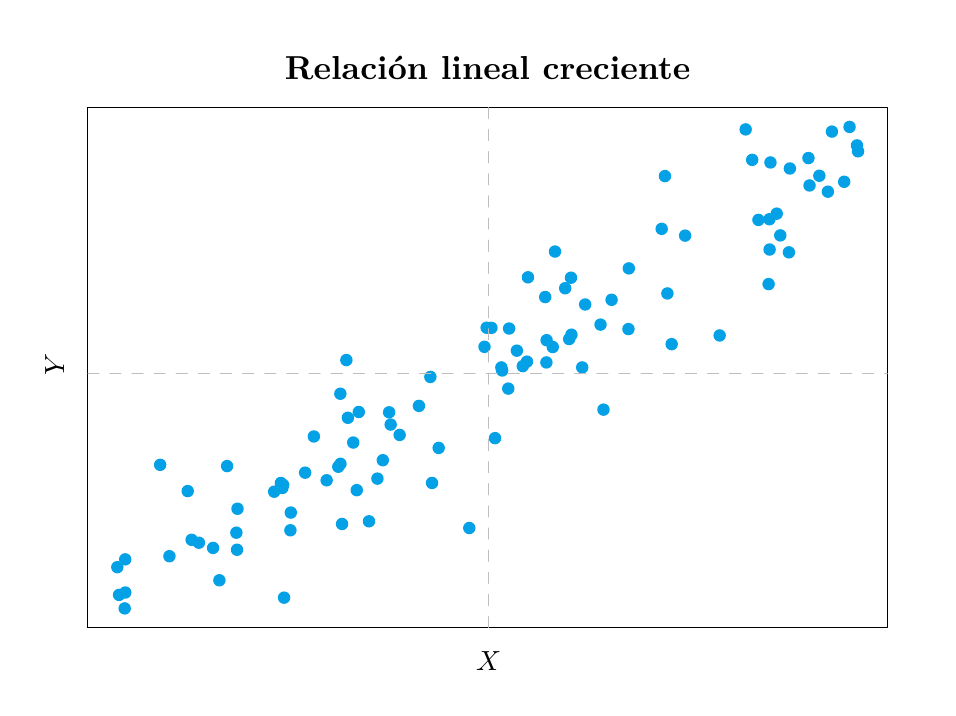
\begin{tikzpicture}[x=1pt,y=1pt]
\definecolor{fillColor}{RGB}{255,255,255}
\path[use as bounding box,fill=fillColor,fill opacity=0.00] (0,0) rectangle (325.21,238.49);
\begin{scope}
\path[clip] ( 21.68, 21.68) rectangle (310.76,209.58);
\definecolor{fillColor}{RGB}{5,161,230}

\path[fill=fillColor] (267.74,145.83) circle (  2.25);

\path[fill=fillColor] (229.09,165.79) circle (  2.25);

\path[fill=fillColor] (112.98,106.21) circle (  2.25);

\path[fill=fillColor] (264.06,169.03) circle (  2.25);

\path[fill=fillColor] (167.57,130.03) circle (  2.25);

\path[fill=fillColor] ( 92.65, 32.53) circle (  2.25);

\path[fill=fillColor] ( 47.87, 80.52) circle (  2.25);

\path[fill=fillColor] ( 33.02, 33.52) circle (  2.25);

\path[fill=fillColor] (187.00,141.15) circle (  2.25);

\path[fill=fillColor] (194.23,144.34) circle (  2.25);

\path[fill=fillColor] ( 95.08, 63.27) circle (  2.25);

\path[fill=fillColor] ( 69.27, 38.81) circle (  2.25);

\path[fill=fillColor] (250.05,127.27) circle (  2.25);

\path[fill=fillColor] (141.38,101.82) circle (  2.25);

\path[fill=fillColor] (189.74,123.09) circle (  2.25);

\path[fill=fillColor] (126.38, 75.54) circle (  2.25);

\path[fill=fillColor] ( 75.82, 64.65) circle (  2.25);

\path[fill=fillColor] (128.33, 82.19) circle (  2.25);

\path[fill=fillColor] (196.33,148.14) circle (  2.25);

\path[fill=fillColor] (100.26, 77.69) circle (  2.25);

\path[fill=fillColor] (282.52,181.47) circle (  2.25);

\path[fill=fillColor] (180.42,117.81) circle (  2.25);

\path[fill=fillColor] ( 75.65, 49.84) circle (  2.25);

\path[fill=fillColor] (113.03, 80.89) circle (  2.25);

\path[fill=fillColor] (275.42,187.60) circle (  2.25);

\path[fill=fillColor] (134.41, 91.33) circle (  2.25);

\path[fill=fillColor] (296.98,202.62) circle (  2.25);

\path[fill=fillColor] (108.04, 74.94) circle (  2.25);

\path[fill=fillColor] (268.04,169.27) circle (  2.25);

\path[fill=fillColor] ( 89.07, 70.81) circle (  2.25);

\path[fill=fillColor] ( 61.87, 52.37) circle (  2.25);

\path[fill=fillColor] ( 59.24, 53.43) circle (  2.25);

\path[fill=fillColor] (123.33, 60.12) circle (  2.25);

\path[fill=fillColor] ( 35.06, 28.64) circle (  2.25);

\path[fill=fillColor] (259.44,201.73) circle (  2.25);

\path[fill=fillColor] (146.11, 73.97) circle (  2.25);

\path[fill=fillColor] (208.07,100.47) circle (  2.25);

\path[fill=fillColor] (112.25, 79.83) circle (  2.25);

\path[fill=fillColor] (103.42, 90.77) circle (  2.25);

\path[fill=fillColor] (237.56,163.34) circle (  2.25);

\path[fill=fillColor] (195.67,125.98) circle (  2.25);

\path[fill=fillColor] (173.66,108.07) circle (  2.25);

\path[fill=fillColor] (290.61,200.94) circle (  2.25);

\path[fill=fillColor] (115.16,118.38) circle (  2.25);

\path[fill=fillColor] (119.65, 99.61) circle (  2.25);

\path[fill=fillColor] ( 57.83, 71.04) circle (  2.25);

\path[fill=fillColor] (113.60, 59.15) circle (  2.25);

\path[fill=fillColor] (217.09,129.58) circle (  2.25);

\path[fill=fillColor] (115.71, 97.52) circle (  2.25);

\path[fill=fillColor] ( 92.32, 73.26) circle (  2.25);

\path[fill=fillColor] (270.67,171.29) circle (  2.25);

\path[fill=fillColor] (268.40,189.78) circle (  2.25);

\path[fill=fillColor] (286.06,184.98) circle (  2.25);

\path[fill=fillColor] (282.13,191.38) circle (  2.25);

\path[fill=fillColor] (200.38,115.72) circle (  2.25);

\path[fill=fillColor] (275.08,157.31) circle (  2.25);

\path[fill=fillColor] (230.28,184.86) circle (  2.25);

\path[fill=fillColor] (187.51,125.55) circle (  2.25);

\path[fill=fillColor] (190.55,157.59) circle (  2.25);

\path[fill=fillColor] (289.16,179.23) circle (  2.25);

\path[fill=fillColor] (196.49,127.54) circle (  2.25);

\path[fill=fillColor] ( 67.00, 50.50) circle (  2.25);

\path[fill=fillColor] (148.51, 86.63) circle (  2.25);

\path[fill=fillColor] (171.16,115.72) circle (  2.25);

\path[fill=fillColor] (210.99,140.16) circle (  2.25);

\path[fill=fillColor] ( 32.39, 43.54) circle (  2.25);

\path[fill=fillColor] ( 94.94, 56.87) circle (  2.25);

\path[fill=fillColor] (176.77,121.78) circle (  2.25);

\path[fill=fillColor] (178.91,116.19) circle (  2.25);

\path[fill=fillColor] (159.58, 57.70) circle (  2.25);

\path[fill=fillColor] ( 72.06, 80.07) circle (  2.25);

\path[fill=fillColor] (201.45,138.46) circle (  2.25);

\path[fill=fillColor] ( 91.50, 73.96) circle (  2.25);

\path[fill=fillColor] (117.65, 88.58) circle (  2.25);

\path[fill=fillColor] (206.99,131.19) circle (  2.25);

\path[fill=fillColor] (271.95,163.43) circle (  2.25);

\path[fill=fillColor] (165.07,123.16) circle (  2.25);

\path[fill=fillColor] (268.09,158.32) circle (  2.25);

\path[fill=fillColor] (261.79,190.72) circle (  2.25);

\path[fill=fillColor] ( 92.03, 72.17) circle (  2.25);

\path[fill=fillColor] ( 75.41, 56.00) circle (  2.25);

\path[fill=fillColor] (217.23,151.51) circle (  2.25);

\path[fill=fillColor] ( 35.27, 34.38) circle (  2.25);

\path[fill=fillColor] (173.96,129.78) circle (  2.25);

\path[fill=fillColor] (231.16,142.45) circle (  2.25);

\path[fill=fillColor] (145.51,112.29) circle (  2.25);

\path[fill=fillColor] (299.67,195.94) circle (  2.25);

\path[fill=fillColor] (168.88, 90.17) circle (  2.25);

\path[fill=fillColor] (165.85,130.07) circle (  2.25);

\path[fill=fillColor] (232.70,124.13) circle (  2.25);

\path[fill=fillColor] (295.04,182.80) circle (  2.25);

\path[fill=fillColor] (187.44,117.52) circle (  2.25);

\path[fill=fillColor] (171.45,114.61) circle (  2.25);

\path[fill=fillColor] (130.61, 99.50) circle (  2.25);

\path[fill=fillColor] (118.92, 71.37) circle (  2.25);

\path[fill=fillColor] (300.05,193.81) circle (  2.25);

\path[fill=fillColor] (180.78,148.28) circle (  2.25);

\path[fill=fillColor] ( 51.22, 47.50) circle (  2.25);

\path[fill=fillColor] (131.17, 95.07) circle (  2.25);

\path[fill=fillColor] ( 35.24, 46.37) circle (  2.25);
\end{scope}
\begin{scope}
\path[clip] (  0.00,  0.00) rectangle (325.21,238.49);
\definecolor{drawColor}{RGB}{0,0,0}

\node[text=drawColor,anchor=base,inner sep=0pt, outer sep=0pt, scale=  1.20] at (166.22,219.84) {\bfseries Relación lineal creciente};

\node[text=drawColor,anchor=base,inner sep=0pt, outer sep=0pt, scale=  1.00] at (166.22,  6.08) {$X$};

\node[text=drawColor,rotate= 90.00,anchor=base,inner sep=0pt, outer sep=0pt, scale=  1.00] at ( 13.28,115.63) {$Y$};
\end{scope}
\begin{scope}
\path[clip] (  0.00,  0.00) rectangle (325.21,238.49);
\definecolor{drawColor}{RGB}{0,0,0}

\path[draw=drawColor,line width= 0.4pt,line join=round,line cap=round] ( 21.68, 21.68) --
	(310.76, 21.68) --
	(310.76,209.58) --
	( 21.68,209.58) --
	( 21.68, 21.68);
\end{scope}
\begin{scope}
\path[clip] ( 21.68, 21.68) rectangle (310.76,209.58);
\definecolor{drawColor}{RGB}{190,190,190}

\path[draw=drawColor,line width= 0.4pt,dash pattern=on 4pt off 4pt ,line join=round,line cap=round] ( 21.68,113.44) -- (310.76,113.44);

\path[draw=drawColor,line width= 0.4pt,dash pattern=on 4pt off 4pt ,line join=round,line cap=round] (166.43, 21.68) -- (166.43,209.58);
\end{scope}
\end{tikzpicture}
}}
\mode<presentation>{\resizebox{0.9\textwidth}{!}{% Created by tikzDevice version 0.10.1 on 2016-02-27 12:54:11
% !TEX encoding = UTF-8 Unicode
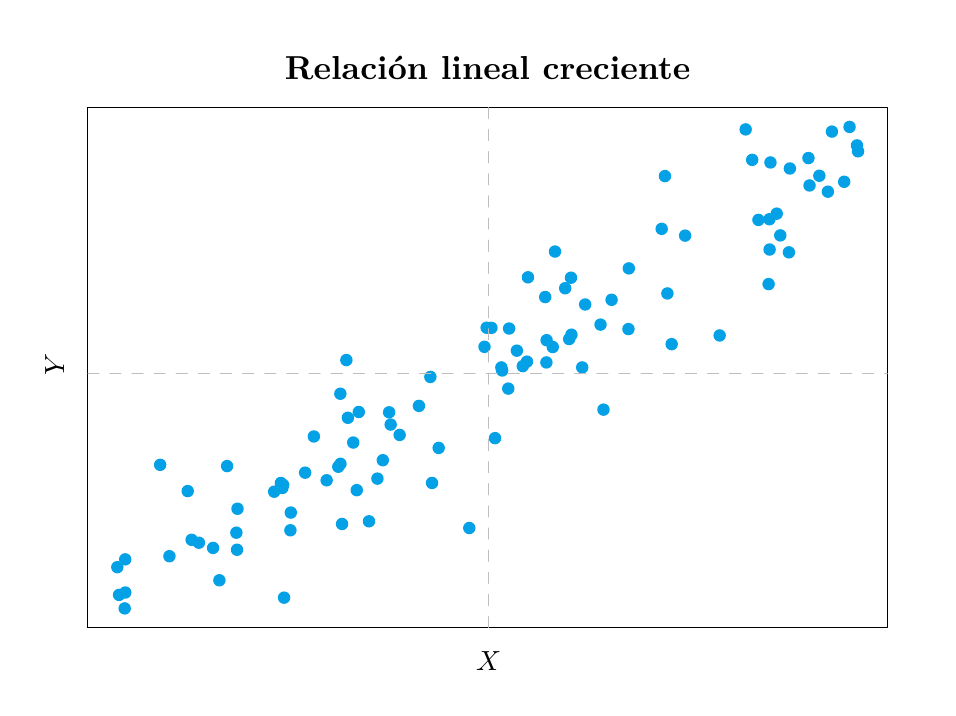
\begin{tikzpicture}[x=1pt,y=1pt]
\definecolor{fillColor}{RGB}{255,255,255}
\path[use as bounding box,fill=fillColor,fill opacity=0.00] (0,0) rectangle (325.21,238.49);
\begin{scope}
\path[clip] ( 21.68, 21.68) rectangle (310.76,209.58);
\definecolor{fillColor}{RGB}{5,161,230}

\path[fill=fillColor] (267.74,145.83) circle (  2.25);

\path[fill=fillColor] (229.09,165.79) circle (  2.25);

\path[fill=fillColor] (112.98,106.21) circle (  2.25);

\path[fill=fillColor] (264.06,169.03) circle (  2.25);

\path[fill=fillColor] (167.57,130.03) circle (  2.25);

\path[fill=fillColor] ( 92.65, 32.53) circle (  2.25);

\path[fill=fillColor] ( 47.87, 80.52) circle (  2.25);

\path[fill=fillColor] ( 33.02, 33.52) circle (  2.25);

\path[fill=fillColor] (187.00,141.15) circle (  2.25);

\path[fill=fillColor] (194.23,144.34) circle (  2.25);

\path[fill=fillColor] ( 95.08, 63.27) circle (  2.25);

\path[fill=fillColor] ( 69.27, 38.81) circle (  2.25);

\path[fill=fillColor] (250.05,127.27) circle (  2.25);

\path[fill=fillColor] (141.38,101.82) circle (  2.25);

\path[fill=fillColor] (189.74,123.09) circle (  2.25);

\path[fill=fillColor] (126.38, 75.54) circle (  2.25);

\path[fill=fillColor] ( 75.82, 64.65) circle (  2.25);

\path[fill=fillColor] (128.33, 82.19) circle (  2.25);

\path[fill=fillColor] (196.33,148.14) circle (  2.25);

\path[fill=fillColor] (100.26, 77.69) circle (  2.25);

\path[fill=fillColor] (282.52,181.47) circle (  2.25);

\path[fill=fillColor] (180.42,117.81) circle (  2.25);

\path[fill=fillColor] ( 75.65, 49.84) circle (  2.25);

\path[fill=fillColor] (113.03, 80.89) circle (  2.25);

\path[fill=fillColor] (275.42,187.60) circle (  2.25);

\path[fill=fillColor] (134.41, 91.33) circle (  2.25);

\path[fill=fillColor] (296.98,202.62) circle (  2.25);

\path[fill=fillColor] (108.04, 74.94) circle (  2.25);

\path[fill=fillColor] (268.04,169.27) circle (  2.25);

\path[fill=fillColor] ( 89.07, 70.81) circle (  2.25);

\path[fill=fillColor] ( 61.87, 52.37) circle (  2.25);

\path[fill=fillColor] ( 59.24, 53.43) circle (  2.25);

\path[fill=fillColor] (123.33, 60.12) circle (  2.25);

\path[fill=fillColor] ( 35.06, 28.64) circle (  2.25);

\path[fill=fillColor] (259.44,201.73) circle (  2.25);

\path[fill=fillColor] (146.11, 73.97) circle (  2.25);

\path[fill=fillColor] (208.07,100.47) circle (  2.25);

\path[fill=fillColor] (112.25, 79.83) circle (  2.25);

\path[fill=fillColor] (103.42, 90.77) circle (  2.25);

\path[fill=fillColor] (237.56,163.34) circle (  2.25);

\path[fill=fillColor] (195.67,125.98) circle (  2.25);

\path[fill=fillColor] (173.66,108.07) circle (  2.25);

\path[fill=fillColor] (290.61,200.94) circle (  2.25);

\path[fill=fillColor] (115.16,118.38) circle (  2.25);

\path[fill=fillColor] (119.65, 99.61) circle (  2.25);

\path[fill=fillColor] ( 57.83, 71.04) circle (  2.25);

\path[fill=fillColor] (113.60, 59.15) circle (  2.25);

\path[fill=fillColor] (217.09,129.58) circle (  2.25);

\path[fill=fillColor] (115.71, 97.52) circle (  2.25);

\path[fill=fillColor] ( 92.32, 73.26) circle (  2.25);

\path[fill=fillColor] (270.67,171.29) circle (  2.25);

\path[fill=fillColor] (268.40,189.78) circle (  2.25);

\path[fill=fillColor] (286.06,184.98) circle (  2.25);

\path[fill=fillColor] (282.13,191.38) circle (  2.25);

\path[fill=fillColor] (200.38,115.72) circle (  2.25);

\path[fill=fillColor] (275.08,157.31) circle (  2.25);

\path[fill=fillColor] (230.28,184.86) circle (  2.25);

\path[fill=fillColor] (187.51,125.55) circle (  2.25);

\path[fill=fillColor] (190.55,157.59) circle (  2.25);

\path[fill=fillColor] (289.16,179.23) circle (  2.25);

\path[fill=fillColor] (196.49,127.54) circle (  2.25);

\path[fill=fillColor] ( 67.00, 50.50) circle (  2.25);

\path[fill=fillColor] (148.51, 86.63) circle (  2.25);

\path[fill=fillColor] (171.16,115.72) circle (  2.25);

\path[fill=fillColor] (210.99,140.16) circle (  2.25);

\path[fill=fillColor] ( 32.39, 43.54) circle (  2.25);

\path[fill=fillColor] ( 94.94, 56.87) circle (  2.25);

\path[fill=fillColor] (176.77,121.78) circle (  2.25);

\path[fill=fillColor] (178.91,116.19) circle (  2.25);

\path[fill=fillColor] (159.58, 57.70) circle (  2.25);

\path[fill=fillColor] ( 72.06, 80.07) circle (  2.25);

\path[fill=fillColor] (201.45,138.46) circle (  2.25);

\path[fill=fillColor] ( 91.50, 73.96) circle (  2.25);

\path[fill=fillColor] (117.65, 88.58) circle (  2.25);

\path[fill=fillColor] (206.99,131.19) circle (  2.25);

\path[fill=fillColor] (271.95,163.43) circle (  2.25);

\path[fill=fillColor] (165.07,123.16) circle (  2.25);

\path[fill=fillColor] (268.09,158.32) circle (  2.25);

\path[fill=fillColor] (261.79,190.72) circle (  2.25);

\path[fill=fillColor] ( 92.03, 72.17) circle (  2.25);

\path[fill=fillColor] ( 75.41, 56.00) circle (  2.25);

\path[fill=fillColor] (217.23,151.51) circle (  2.25);

\path[fill=fillColor] ( 35.27, 34.38) circle (  2.25);

\path[fill=fillColor] (173.96,129.78) circle (  2.25);

\path[fill=fillColor] (231.16,142.45) circle (  2.25);

\path[fill=fillColor] (145.51,112.29) circle (  2.25);

\path[fill=fillColor] (299.67,195.94) circle (  2.25);

\path[fill=fillColor] (168.88, 90.17) circle (  2.25);

\path[fill=fillColor] (165.85,130.07) circle (  2.25);

\path[fill=fillColor] (232.70,124.13) circle (  2.25);

\path[fill=fillColor] (295.04,182.80) circle (  2.25);

\path[fill=fillColor] (187.44,117.52) circle (  2.25);

\path[fill=fillColor] (171.45,114.61) circle (  2.25);

\path[fill=fillColor] (130.61, 99.50) circle (  2.25);

\path[fill=fillColor] (118.92, 71.37) circle (  2.25);

\path[fill=fillColor] (300.05,193.81) circle (  2.25);

\path[fill=fillColor] (180.78,148.28) circle (  2.25);

\path[fill=fillColor] ( 51.22, 47.50) circle (  2.25);

\path[fill=fillColor] (131.17, 95.07) circle (  2.25);

\path[fill=fillColor] ( 35.24, 46.37) circle (  2.25);
\end{scope}
\begin{scope}
\path[clip] (  0.00,  0.00) rectangle (325.21,238.49);
\definecolor{drawColor}{RGB}{0,0,0}

\node[text=drawColor,anchor=base,inner sep=0pt, outer sep=0pt, scale=  1.20] at (166.22,219.84) {\bfseries Relación lineal creciente};

\node[text=drawColor,anchor=base,inner sep=0pt, outer sep=0pt, scale=  1.00] at (166.22,  6.08) {$X$};

\node[text=drawColor,rotate= 90.00,anchor=base,inner sep=0pt, outer sep=0pt, scale=  1.00] at ( 13.28,115.63) {$Y$};
\end{scope}
\begin{scope}
\path[clip] (  0.00,  0.00) rectangle (325.21,238.49);
\definecolor{drawColor}{RGB}{0,0,0}

\path[draw=drawColor,line width= 0.4pt,line join=round,line cap=round] ( 21.68, 21.68) --
	(310.76, 21.68) --
	(310.76,209.58) --
	( 21.68,209.58) --
	( 21.68, 21.68);
\end{scope}
\begin{scope}
\path[clip] ( 21.68, 21.68) rectangle (310.76,209.58);
\definecolor{drawColor}{RGB}{190,190,190}

\path[draw=drawColor,line width= 0.4pt,dash pattern=on 4pt off 4pt ,line join=round,line cap=round] ( 21.68,113.44) -- (310.76,113.44);

\path[draw=drawColor,line width= 0.4pt,dash pattern=on 4pt off 4pt ,line join=round,line cap=round] (166.43, 21.68) -- (166.43,209.58);
\end{scope}
\end{tikzpicture}
}}

\[
\sum(x_i-\bar x)(y_j-\bar y) = +
\]
\end{column}
\begin{column}{0.5\textwidth}
Si la relación entre las variables es \emph{lineal y decreciente}, entonces la mayor parte de los puntos estarán en los cuadrantes 2 y 4 y la suma de los productos de desviaciones será negativa.

\centering
\tikzsetnextfilename{regresion/diagrama_dispersion_lineal_decreciente}
\mode<article>{\resizebox{0.6\textwidth}{!}{% Created by tikzDevice version 0.10.1 on 2016-02-27 12:54:12
% !TEX encoding = UTF-8 Unicode
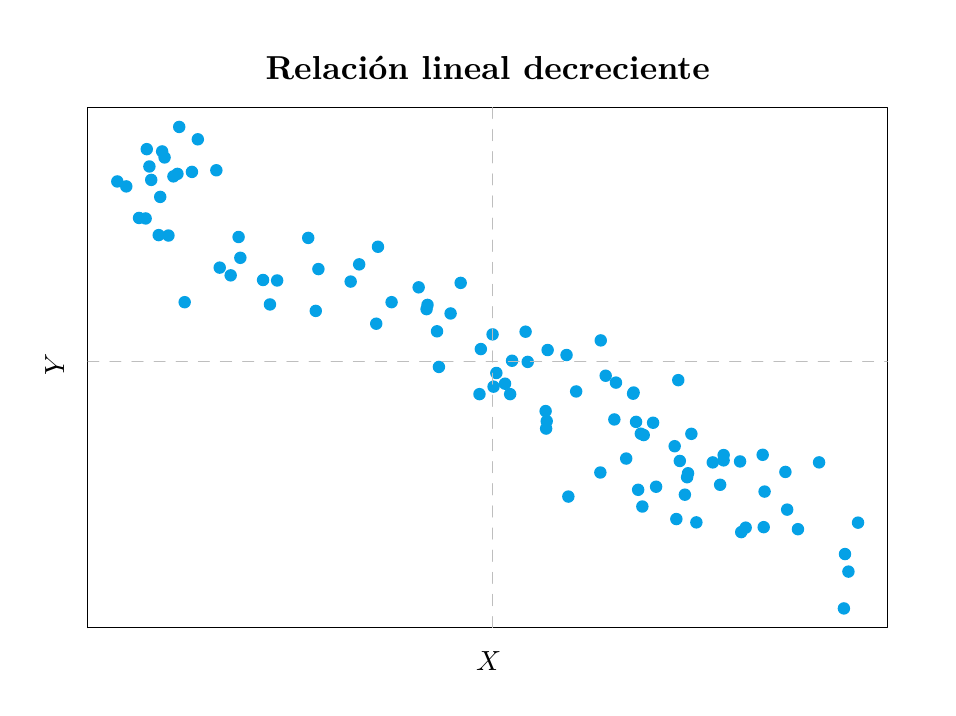
\begin{tikzpicture}[x=1pt,y=1pt]
\definecolor{fillColor}{RGB}{255,255,255}
\path[use as bounding box,fill=fillColor,fill opacity=0.00] (0,0) rectangle (325.21,238.49);
\begin{scope}
\path[clip] ( 21.68, 21.68) rectangle (310.76,209.58);
\definecolor{fillColor}{RGB}{5,161,230}

\path[fill=fillColor] (257.84, 56.21) circle (  2.25);

\path[fill=fillColor] (247.55, 81.40) circle (  2.25);

\path[fill=fillColor] (172.49,109.84) circle (  2.25);

\path[fill=fillColor] (180.69,117.72) circle (  2.25);

\path[fill=fillColor] (207.08,125.48) circle (  2.25);

\path[fill=fillColor] (187.55, 96.32) circle (  2.25);

\path[fill=fillColor] (156.46,146.27) circle (  2.25);

\path[fill=fillColor] ( 35.63,181.13) circle (  2.25);

\path[fill=fillColor] (222.11, 65.46) circle (  2.25);

\path[fill=fillColor] ( 73.35,148.99) circle (  2.25);

\path[fill=fillColor] (167.99,127.66) circle (  2.25);

\path[fill=fillColor] ( 47.35,163.54) circle (  2.25);

\path[fill=fillColor] (233.79, 87.25) circle (  2.25);

\path[fill=fillColor] (194.72,120.20) circle (  2.25);

\path[fill=fillColor] (104.10,136.14) circle (  2.25);

\path[fill=fillColor] ( 48.59,193.77) circle (  2.25);

\path[fill=fillColor] (273.80, 77.96) circle (  2.25);

\path[fill=fillColor] ( 42.63,169.55) circle (  2.25);

\path[fill=fillColor] (219.84, 96.04) circle (  2.25);

\path[fill=fillColor] (195.37, 69.05) circle (  2.25);

\path[fill=fillColor] (152.82,135.22) circle (  2.25);

\path[fill=fillColor] (169.36,113.71) circle (  2.25);

\path[fill=fillColor] (265.96, 58.00) circle (  2.25);

\path[fill=fillColor] (296.58, 41.94) circle (  2.25);

\path[fill=fillColor] (147.92,128.77) circle (  2.25);

\path[fill=fillColor] ( 43.03,194.59) circle (  2.25);

\path[fill=fillColor] (105.05,151.26) circle (  2.25);

\path[fill=fillColor] ( 59.35,186.37) circle (  2.25);

\path[fill=fillColor] ( 50.87,163.38) circle (  2.25);

\path[fill=fillColor] ( 43.98,188.33) circle (  2.25);

\path[fill=fillColor] (218.95,106.65) circle (  2.25);

\path[fill=fillColor] (250.22, 73.32) circle (  2.25);

\path[fill=fillColor] (119.79,152.96) circle (  2.25);

\path[fill=fillColor] (116.71,146.74) circle (  2.25);

\path[fill=fillColor] (251.49, 84.05) circle (  2.25);

\path[fill=fillColor] ( 44.65,183.48) circle (  2.25);

\path[fill=fillColor] ( 61.48,198.15) circle (  2.25);

\path[fill=fillColor] (222.61, 91.28) circle (  2.25);

\path[fill=fillColor] (266.28, 70.86) circle (  2.25);

\path[fill=fillColor] (126.58,159.32) circle (  2.25);

\path[fill=fillColor] ( 54.76,202.62) circle (  2.25);

\path[fill=fillColor] (251.47, 82.13) circle (  2.25);

\path[fill=fillColor] (144.14,136.78) circle (  2.25);

\path[fill=fillColor] (144.48,138.31) circle (  2.25);

\path[fill=fillColor] (216.27, 82.79) circle (  2.25);

\path[fill=fillColor] ( 47.89,177.34) circle (  2.25);

\path[fill=fillColor] (175.03,118.13) circle (  2.25);

\path[fill=fillColor] (274.44, 64.34) circle (  2.25);

\path[fill=fillColor] (163.26,106.07) circle (  2.25);

\path[fill=fillColor] (148.60,115.90) circle (  2.25);

\path[fill=fillColor] ( 90.15,147.14) circle (  2.25);

\path[fill=fillColor] ( 49.47,191.59) circle (  2.25);

\path[fill=fillColor] (218.77,106.23) circle (  2.25);

\path[fill=fillColor] (300.05, 59.63) circle (  2.25);

\path[fill=fillColor] (101.37,162.52) circle (  2.25);

\path[fill=fillColor] ( 76.21,162.85) circle (  2.25);

\path[fill=fillColor] (241.63, 59.72) circle (  2.25);

\path[fill=fillColor] (259.45, 57.82) circle (  2.25);

\path[fill=fillColor] (235.65, 81.92) circle (  2.25);

\path[fill=fillColor] (221.56, 91.77) circle (  2.25);

\path[fill=fillColor] (187.34, 93.63) circle (  2.25);

\path[fill=fillColor] ( 76.85,155.33) circle (  2.25);

\path[fill=fillColor] (285.97, 81.41) circle (  2.25);

\path[fill=fillColor] (212.58,110.24) circle (  2.25);

\path[fill=fillColor] (206.94, 77.75) circle (  2.25);

\path[fill=fillColor] ( 40.24,169.73) circle (  2.25);

\path[fill=fillColor] ( 87.55,138.48) circle (  2.25);

\path[fill=fillColor] ( 32.39,182.92) circle (  2.25);

\path[fill=fillColor] ( 52.67,184.75) circle (  2.25);

\path[fill=fillColor] (278.34, 57.27) circle (  2.25);

\path[fill=fillColor] (257.42, 81.74) circle (  2.25);

\path[fill=fillColor] ( 69.39,151.78) circle (  2.25);

\path[fill=fillColor] (187.16, 99.94) circle (  2.25);

\path[fill=fillColor] (198.20,107.04) circle (  2.25);

\path[fill=fillColor] (220.59, 71.50) circle (  2.25);

\path[fill=fillColor] (238.28, 76.05) circle (  2.25);

\path[fill=fillColor] (131.50,139.30) circle (  2.25);

\path[fill=fillColor] (227.08, 72.61) circle (  2.25);

\path[fill=fillColor] (141.28,144.66) circle (  2.25);

\path[fill=fillColor] (163.75,122.35) circle (  2.25);

\path[fill=fillColor] ( 68.17,186.96) circle (  2.25);

\path[fill=fillColor] (265.59, 84.15) circle (  2.25);

\path[fill=fillColor] ( 85.06,147.31) circle (  2.25);

\path[fill=fillColor] (168.35,108.77) circle (  2.25);

\path[fill=fillColor] (211.99, 96.92) circle (  2.25);

\path[fill=fillColor] (174.34,106.07) circle (  2.25);

\path[fill=fillColor] ( 56.73,139.29) circle (  2.25);

\path[fill=fillColor] (294.94, 28.64) circle (  2.25);

\path[fill=fillColor] (225.99, 95.73) circle (  2.25);

\path[fill=fillColor] (239.82, 91.72) circle (  2.25);

\path[fill=fillColor] (237.48, 69.74) circle (  2.25);

\path[fill=fillColor] (187.89,122.01) circle (  2.25);

\path[fill=fillColor] (295.34, 48.28) circle (  2.25);

\path[fill=fillColor] (208.86,112.72) circle (  2.25);

\path[fill=fillColor] ( 54.11,185.66) circle (  2.25);

\path[fill=fillColor] (235.09,111.12) circle (  2.25);

\path[fill=fillColor] (234.40, 60.93) circle (  2.25);

\path[fill=fillColor] (179.92,128.63) circle (  2.25);

\path[fill=fillColor] (125.95,131.52) circle (  2.25);

\path[fill=fillColor] (238.62, 77.48) circle (  2.25);
\end{scope}
\begin{scope}
\path[clip] (  0.00,  0.00) rectangle (325.21,238.49);
\definecolor{drawColor}{RGB}{0,0,0}

\node[text=drawColor,anchor=base,inner sep=0pt, outer sep=0pt, scale=  1.20] at (166.22,219.84) {\bfseries Relación lineal decreciente};

\node[text=drawColor,anchor=base,inner sep=0pt, outer sep=0pt, scale=  1.00] at (166.22,  6.08) {$X$};

\node[text=drawColor,rotate= 90.00,anchor=base,inner sep=0pt, outer sep=0pt, scale=  1.00] at ( 13.28,115.63) {$Y$};
\end{scope}
\begin{scope}
\path[clip] (  0.00,  0.00) rectangle (325.21,238.49);
\definecolor{drawColor}{RGB}{0,0,0}

\path[draw=drawColor,line width= 0.4pt,line join=round,line cap=round] ( 21.68, 21.68) --
	(310.76, 21.68) --
	(310.76,209.58) --
	( 21.68,209.58) --
	( 21.68, 21.68);
\end{scope}
\begin{scope}
\path[clip] ( 21.68, 21.68) rectangle (310.76,209.58);
\definecolor{drawColor}{RGB}{190,190,190}

\path[draw=drawColor,line width= 0.4pt,dash pattern=on 4pt off 4pt ,line join=round,line cap=round] ( 21.68,117.96) -- (310.76,117.96);

\path[draw=drawColor,line width= 0.4pt,dash pattern=on 4pt off 4pt ,line join=round,line cap=round] (167.81, 21.68) -- (167.81,209.58);
\end{scope}
\end{tikzpicture}
}}
\mode<presentation>{\resizebox{0.9\textwidth}{!}{% Created by tikzDevice version 0.10.1 on 2016-02-27 12:54:12
% !TEX encoding = UTF-8 Unicode
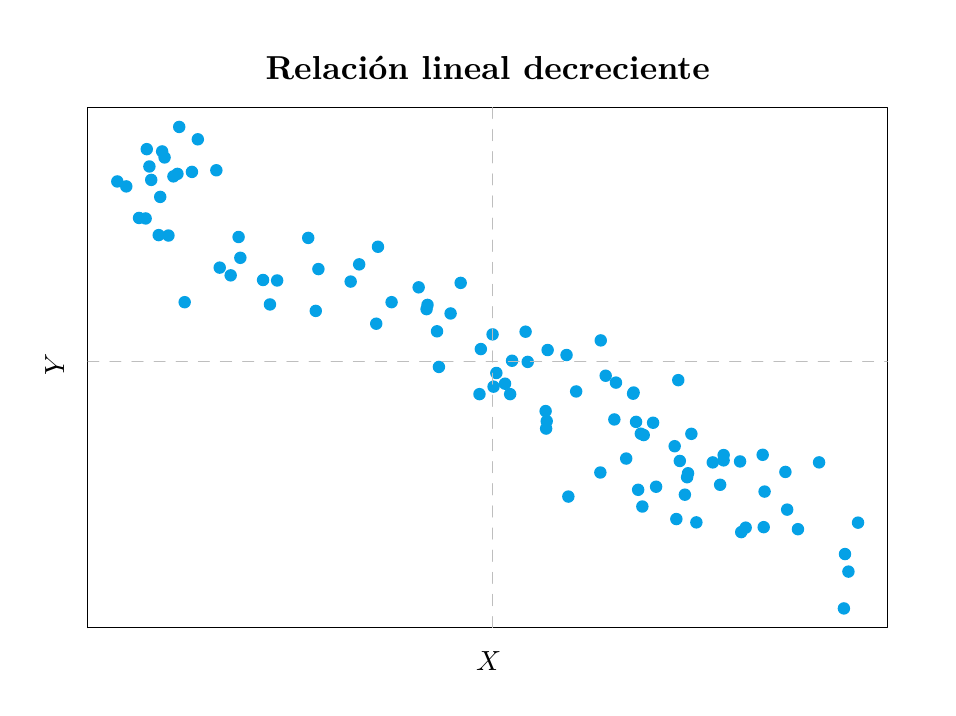
\begin{tikzpicture}[x=1pt,y=1pt]
\definecolor{fillColor}{RGB}{255,255,255}
\path[use as bounding box,fill=fillColor,fill opacity=0.00] (0,0) rectangle (325.21,238.49);
\begin{scope}
\path[clip] ( 21.68, 21.68) rectangle (310.76,209.58);
\definecolor{fillColor}{RGB}{5,161,230}

\path[fill=fillColor] (257.84, 56.21) circle (  2.25);

\path[fill=fillColor] (247.55, 81.40) circle (  2.25);

\path[fill=fillColor] (172.49,109.84) circle (  2.25);

\path[fill=fillColor] (180.69,117.72) circle (  2.25);

\path[fill=fillColor] (207.08,125.48) circle (  2.25);

\path[fill=fillColor] (187.55, 96.32) circle (  2.25);

\path[fill=fillColor] (156.46,146.27) circle (  2.25);

\path[fill=fillColor] ( 35.63,181.13) circle (  2.25);

\path[fill=fillColor] (222.11, 65.46) circle (  2.25);

\path[fill=fillColor] ( 73.35,148.99) circle (  2.25);

\path[fill=fillColor] (167.99,127.66) circle (  2.25);

\path[fill=fillColor] ( 47.35,163.54) circle (  2.25);

\path[fill=fillColor] (233.79, 87.25) circle (  2.25);

\path[fill=fillColor] (194.72,120.20) circle (  2.25);

\path[fill=fillColor] (104.10,136.14) circle (  2.25);

\path[fill=fillColor] ( 48.59,193.77) circle (  2.25);

\path[fill=fillColor] (273.80, 77.96) circle (  2.25);

\path[fill=fillColor] ( 42.63,169.55) circle (  2.25);

\path[fill=fillColor] (219.84, 96.04) circle (  2.25);

\path[fill=fillColor] (195.37, 69.05) circle (  2.25);

\path[fill=fillColor] (152.82,135.22) circle (  2.25);

\path[fill=fillColor] (169.36,113.71) circle (  2.25);

\path[fill=fillColor] (265.96, 58.00) circle (  2.25);

\path[fill=fillColor] (296.58, 41.94) circle (  2.25);

\path[fill=fillColor] (147.92,128.77) circle (  2.25);

\path[fill=fillColor] ( 43.03,194.59) circle (  2.25);

\path[fill=fillColor] (105.05,151.26) circle (  2.25);

\path[fill=fillColor] ( 59.35,186.37) circle (  2.25);

\path[fill=fillColor] ( 50.87,163.38) circle (  2.25);

\path[fill=fillColor] ( 43.98,188.33) circle (  2.25);

\path[fill=fillColor] (218.95,106.65) circle (  2.25);

\path[fill=fillColor] (250.22, 73.32) circle (  2.25);

\path[fill=fillColor] (119.79,152.96) circle (  2.25);

\path[fill=fillColor] (116.71,146.74) circle (  2.25);

\path[fill=fillColor] (251.49, 84.05) circle (  2.25);

\path[fill=fillColor] ( 44.65,183.48) circle (  2.25);

\path[fill=fillColor] ( 61.48,198.15) circle (  2.25);

\path[fill=fillColor] (222.61, 91.28) circle (  2.25);

\path[fill=fillColor] (266.28, 70.86) circle (  2.25);

\path[fill=fillColor] (126.58,159.32) circle (  2.25);

\path[fill=fillColor] ( 54.76,202.62) circle (  2.25);

\path[fill=fillColor] (251.47, 82.13) circle (  2.25);

\path[fill=fillColor] (144.14,136.78) circle (  2.25);

\path[fill=fillColor] (144.48,138.31) circle (  2.25);

\path[fill=fillColor] (216.27, 82.79) circle (  2.25);

\path[fill=fillColor] ( 47.89,177.34) circle (  2.25);

\path[fill=fillColor] (175.03,118.13) circle (  2.25);

\path[fill=fillColor] (274.44, 64.34) circle (  2.25);

\path[fill=fillColor] (163.26,106.07) circle (  2.25);

\path[fill=fillColor] (148.60,115.90) circle (  2.25);

\path[fill=fillColor] ( 90.15,147.14) circle (  2.25);

\path[fill=fillColor] ( 49.47,191.59) circle (  2.25);

\path[fill=fillColor] (218.77,106.23) circle (  2.25);

\path[fill=fillColor] (300.05, 59.63) circle (  2.25);

\path[fill=fillColor] (101.37,162.52) circle (  2.25);

\path[fill=fillColor] ( 76.21,162.85) circle (  2.25);

\path[fill=fillColor] (241.63, 59.72) circle (  2.25);

\path[fill=fillColor] (259.45, 57.82) circle (  2.25);

\path[fill=fillColor] (235.65, 81.92) circle (  2.25);

\path[fill=fillColor] (221.56, 91.77) circle (  2.25);

\path[fill=fillColor] (187.34, 93.63) circle (  2.25);

\path[fill=fillColor] ( 76.85,155.33) circle (  2.25);

\path[fill=fillColor] (285.97, 81.41) circle (  2.25);

\path[fill=fillColor] (212.58,110.24) circle (  2.25);

\path[fill=fillColor] (206.94, 77.75) circle (  2.25);

\path[fill=fillColor] ( 40.24,169.73) circle (  2.25);

\path[fill=fillColor] ( 87.55,138.48) circle (  2.25);

\path[fill=fillColor] ( 32.39,182.92) circle (  2.25);

\path[fill=fillColor] ( 52.67,184.75) circle (  2.25);

\path[fill=fillColor] (278.34, 57.27) circle (  2.25);

\path[fill=fillColor] (257.42, 81.74) circle (  2.25);

\path[fill=fillColor] ( 69.39,151.78) circle (  2.25);

\path[fill=fillColor] (187.16, 99.94) circle (  2.25);

\path[fill=fillColor] (198.20,107.04) circle (  2.25);

\path[fill=fillColor] (220.59, 71.50) circle (  2.25);

\path[fill=fillColor] (238.28, 76.05) circle (  2.25);

\path[fill=fillColor] (131.50,139.30) circle (  2.25);

\path[fill=fillColor] (227.08, 72.61) circle (  2.25);

\path[fill=fillColor] (141.28,144.66) circle (  2.25);

\path[fill=fillColor] (163.75,122.35) circle (  2.25);

\path[fill=fillColor] ( 68.17,186.96) circle (  2.25);

\path[fill=fillColor] (265.59, 84.15) circle (  2.25);

\path[fill=fillColor] ( 85.06,147.31) circle (  2.25);

\path[fill=fillColor] (168.35,108.77) circle (  2.25);

\path[fill=fillColor] (211.99, 96.92) circle (  2.25);

\path[fill=fillColor] (174.34,106.07) circle (  2.25);

\path[fill=fillColor] ( 56.73,139.29) circle (  2.25);

\path[fill=fillColor] (294.94, 28.64) circle (  2.25);

\path[fill=fillColor] (225.99, 95.73) circle (  2.25);

\path[fill=fillColor] (239.82, 91.72) circle (  2.25);

\path[fill=fillColor] (237.48, 69.74) circle (  2.25);

\path[fill=fillColor] (187.89,122.01) circle (  2.25);

\path[fill=fillColor] (295.34, 48.28) circle (  2.25);

\path[fill=fillColor] (208.86,112.72) circle (  2.25);

\path[fill=fillColor] ( 54.11,185.66) circle (  2.25);

\path[fill=fillColor] (235.09,111.12) circle (  2.25);

\path[fill=fillColor] (234.40, 60.93) circle (  2.25);

\path[fill=fillColor] (179.92,128.63) circle (  2.25);

\path[fill=fillColor] (125.95,131.52) circle (  2.25);

\path[fill=fillColor] (238.62, 77.48) circle (  2.25);
\end{scope}
\begin{scope}
\path[clip] (  0.00,  0.00) rectangle (325.21,238.49);
\definecolor{drawColor}{RGB}{0,0,0}

\node[text=drawColor,anchor=base,inner sep=0pt, outer sep=0pt, scale=  1.20] at (166.22,219.84) {\bfseries Relación lineal decreciente};

\node[text=drawColor,anchor=base,inner sep=0pt, outer sep=0pt, scale=  1.00] at (166.22,  6.08) {$X$};

\node[text=drawColor,rotate= 90.00,anchor=base,inner sep=0pt, outer sep=0pt, scale=  1.00] at ( 13.28,115.63) {$Y$};
\end{scope}
\begin{scope}
\path[clip] (  0.00,  0.00) rectangle (325.21,238.49);
\definecolor{drawColor}{RGB}{0,0,0}

\path[draw=drawColor,line width= 0.4pt,line join=round,line cap=round] ( 21.68, 21.68) --
	(310.76, 21.68) --
	(310.76,209.58) --
	( 21.68,209.58) --
	( 21.68, 21.68);
\end{scope}
\begin{scope}
\path[clip] ( 21.68, 21.68) rectangle (310.76,209.58);
\definecolor{drawColor}{RGB}{190,190,190}

\path[draw=drawColor,line width= 0.4pt,dash pattern=on 4pt off 4pt ,line join=round,line cap=round] ( 21.68,117.96) -- (310.76,117.96);

\path[draw=drawColor,line width= 0.4pt,dash pattern=on 4pt off 4pt ,line join=round,line cap=round] (167.81, 21.68) -- (167.81,209.58);
\end{scope}
\end{tikzpicture}
}}

\[
\sum(x_i-\bar x)(y_j-\bar y) = -
\]
\end{column}
\end{columns}

\note{Si la relación entre las variables es lineal y creciente, como refleja el primer diagrama de dispersión, entonces la mayor parte de
los puntos estarán en los cuadrantes 1 y 3, y por tanto habrá muchos más puntos cuyo producto de desviaciones sea positivo, que puntos
cuyo producto de desviaciones sea negativo, de manera que la suma de los productos de desviaciones de todos los puntos será positiva.

Por contra, cuando la relación entre las variables sea lineal y decreciente, como ocurre en el segundo diagrama, entonces la la mayor parte de
los puntos estarán en los cuadrantes 2 y 4, y por tanto habrá muchos más puntos cuyo producto de desviaciones sea negativo, que puntos
cuyo producto de desviaciones sea positivo, de manera que la suma de los productos de desviaciones de todos los puntos será negativa.
}
\end{frame}


%---------------------------------------------------------------------slide----
\begin{frame}
\frametitle{Covarianza}
Usando el producto de las desviaciones respecto de las medias surge el siguiente estadístico.

\begin{definicion}[Covarianza muestral]
La \emph{covarianza muestral} de una variable aleatoria bidimensional $(X,Y)$ se define como el promedio de los
productos de las respectivas desviaciones respecto de las medias de $X$ e $Y$.
\[
s_{xy}=\frac{\sum (x_i-\bar x)(y_j-\bar y)n_{ij}}{n}
\]
\end{definicion}
También puede calcularse de manera más sencilla mediante la fórmula
\[
s_{xy}=\frac{\sum x_iy_jn_{ij}}{n}-\bar x\bar y.
\]
La covarianza sirve para estudiar la relación lineal entre dos variables:
\begin{itemize}
\item Si $s_{xy}>0$ existe una relación lineal creciente entre las variables.
\item Si $s_{xy}<0$ existe una relación lineal decreciente entre las variables.
\item Si $s_{xy}=0$ no existe relación lineal entre las variables. 
\end{itemize} 

\note{Del razonamiento anterior surge un estadístico conocido como covarianza para estudiar la relación lineal entre variables.

La covarianza, que se representa $s_{xy}$ se define como la suma de los productos de las desviaciones a las respectivas medias,
multiplicadas por la frecuencia absoluta relativa de cada par y dividido por el tamaño de la muestra.

Si se desarrolla el producto de las desviaciones y se simplifica, se llega a una fórmula equivalente para el cálculo de la covarianza que
consiste en sumar los productos del valor de $X$ por el valor de $Y$ en cada individuo, por la frecuencia absoluta del par, dividido por el
tamaño de la muestra y restarle al cociente el producto de las medias de $X$ e $Y$. Esta fórmula es un poco más fácil de aplicar y por
tanto será la que utilizaremos a lo largo del tema.

A la hora de interpretar la covarianza como medida de relación lineal, lo más importante es su signo, ya que como vimos antes, si existe
relación lineal creciente entre las variables, la suma de los productos de las desviaciones será positiva y también lo será la
covarianza; si la relación es lineal decreciente, la suma de los productos de las desviaciones será negativa y también lo será la
covarianza; mientras que si no hay relación lineal, los puntos se distribuirán más o menos por igual en los cuatro cuadrantes y se
compensarán los productos de desviaciones positivos con los negativos, con lo que la covarianza valdrá aproximadamente 0.

Hay que tener en cuenta que la covarianza tiene unidades, que son el producto de las unidades de $X$ e $Y$, lo cual dificulta su
interpretación a la hora de valorar el grado de dependencia lineal entre las variables, aunque, como veremos más adelante, a partir de ella
es posible obtener una medida adimensional que si permitirá estudiar el grado de dependencia lineal.}
\end{frame}


%---------------------------------------------------------------------slide----
\begin{frame}
\frametitle{Cálculo de la covarianza}
\framesubtitle{Ejemplo con estaturas y pesos}
En el ejemplo de las estaturas y pesos, teniendo en cuenta que 
\[
\begin{array}{|c||c|c|c|c|c|c|c|}
\hline
  X/Y & [50,60) & [60,70) & [70,80) & [80,90) & [90,100) & [100,110) & n_x\\
  \hline\hline
  (150,160] & 2 & 0 & 0 & 0 & 0 & 0 & 2\\
  \hline
  (160,170] & 4 & 4 & 0 & 0 & 0 & 0 & 8\\
  \hline
  (170,180] & 1 & 6 & 3 & 1 & 0 & 0 & 11 \\
  \hline
  (180,190] & 0 & 1 & 4 & 1 & 1 & 0 & 7 \\
  \hline
  (190,200] & 0 & 0 & 0 & 0 & 1 & 1 & 2\\
  \hline
  n_y & 7 & 11 & 7 & 2 & 2 & 1 & 30\\
  \hline
\end{array}
\]
\[
\bar x = 174.67 \mbox{ cm} \qquad \bar y = 69.67 \mbox{ Kg} 
\]
la covarianza vale
\begin{align*}
s_{xy} &=\frac{\sum x_iy_jn_{ij}}{n}-\bar x\bar y =  \frac{155\cdot 55\cdot 2 + 165\cdot 55\cdot 4 + \cdots + 195\cdot 105\cdot 1}{30}-174.67\cdot 69.67 =\\
& = \frac{368200}{30}-12169.26 = 104.07 \mbox{ cm$\cdot$ Kg},
\end{align*}
lo que indica que existe una relación lineal creciente entre la estatura y el peso. 

\note{En el ejemplo de las estaturas y los pesos, para calcular la covarianza a partir de la tabla de frecuencias bidimensional, iremos
sumando el producto de la componente $X$ por la componente $Y$ por su frecuencia absoluta para cada posible par. Como en este caso, además,
los datos se habían agrupado en intervalos, a la hora de hacer estos productos tomaremos las marcas de cada clase, es decir, para el primer
par, correspondiente al intervalo $(150,160]$ de estatura y $[50,60)$ de peso, haremos el producto de 155 que es la marca de clase del
intervalo de la estatura, por 55 que es la marca de clase del intervalo del peso, por su frecuencia absoluta que es 2. A continuación vamos
calculando el resto de productos de igual modo. 155 por 65 y por su frecuencia que es 0, lo que nos da 0, etc. Una vez calculados los
productos se suman, lo que da 368200, esto se divide por el tamaño de la muestra que era 30 y al resultado del cociente se le resta el
producto de las medias que eran $174.67$ cm y $69.67$ kg, lo que nos da una covarianza de $104.07$ cm por kg.

Esto indica que existe una relación lineal creciente entre el peso y la estatura, es decir, que a mayor estatura le corresponde mayor peso
y a mayor peso le corresponde mayor estatura, aunque resulta complicado establecer si esa relación es fuerte o débil ya que no es fácil
interpretar las unidades de cm por kg.}
\end{frame}


\subsection{Regresión}
%---------------------------------------------------------------------slide----
\begin{frame}
\frametitle{Regresión}
En muchos casos el objetivo de un estudio no es solo detectar una relación entre dos variables, sino explicarla mediante alguna función matemática
\[y=f(x)\]
que permita predecir la variable dependiente para cada valor de la independiente.

La \highlight{regresion} es la parte de la Estadística encargada de construir esta función, que se conoce como \highlight{función de regresión} o \highlight{odelo de regresión}.

\note{En muchos casos el objetivo de un estudio no es solo detectar si existe cierta relación entre variables, sino explicarla mediante
alguna función matemática.

De esto se encarga la regresión que trata de buscar un modelo funcional que explique lo mejor posible la relación entre una variable
dependiente $Y$ y un conjunto de variables independientes $X_1,\ldots,X_n$. 

El caso más simple, y el que estudiaremos aquí, es cuando sólo hay una variable independiente $X$ y entonces el modelo es una función de una
sóla variable $y=f(x)$ que se conoce como función de regresión simple.
}
\end{frame}


%---------------------------------------------------------------------slide----
\begin{frame}
\frametitle{Modelos de regresión simple}
Dependiendo de la forma de función de regresión, existen muchos tipos de regresión simple. 
Los más habituales son los que aparecen en la siguiente tabla:
\begin{center}
\mode<presentation>{\rowcolors{1}{red!20}{red!10}}
\begin{tabular}{|l|c|}
\hline
 Familia de curvas       &     Ecuación genérica      \\
\hline\hline
 Lineal                  &          $y=a+bx$          \\
\hline
 Parabólica              &       $y=a+bx+cx^2$        \\
\hline
 Polinómica de grado $n$ & $y=a_0+a_1x+\cdots+a_nx^n$ \\
\hline
 Potencial               &       $y=a\cdot x^b$       \\
\hline
 Exponencial             &     $y=a\cdot e^{bx}$      \\
\hline
 Logarítmica             &       $y=a+b\log x$        \\
\hline
 Inverso                 &       $y = a+\frac{b}{x}$  \\
\hline
 Curva S                 &      $y= e^{a+\frac{b}{x}}$ \\
\hline
\end{tabular}
\end{center}

La elección de un tipo u otro depende de la forma que tenga la nube de puntos del diagrama de dispersión. 

\note{Dependiendo de la forma de función de regresión, existen muchos tipos de regresión simple. Los más habituales son:
\begin{enumerate}
\item El modelo lineal, en el que la función de regresión es una recta.
\item El modelo parabólico, en el que la función de regresión es una parabola, es decir, un polinomio de grado 2.
\item El modelo polinómico de grado $n$, en el que la función de regresión es un polinomio de grado $n$.
\item El modelo potencial, en el que la función de regresión es una función potencial donde el exponente puede ser un númro no entero.
\item El modelo exponencia, en el que la función de regresión es una función exponencial, habitualmente de base $e$, la constante de Euler,
y donde la variable independiente aparece en el exponente.
\item El modelo logarítmico, en el que la función de regresión es una función logarítmica.
\item El modelo inverso, en el que en la función de regresión la variable independiente aparece dividiendo a una constante.
\item Y el modelo de curva S o sigmoidal, que es una combinación del modelo exponencial e inverso.
\end{enumerate}

A la hora de decidir qué modelo construir habrá que tener en cuenta la forma que tenga la nube de puntos del diagrama de dispersión.
}
\end{frame}


%---------------------------------------------------------------------slide----
\begin{frame}
\frametitle{Residuos o errores predictivos}
Una vez elegida la familia de curvas que mejor se adapta a la nube de puntos, se determina, dentro de dicha familia, la curva que mejor se ajusta a la distribución, es decir, la función que mejor predice la variable dependiente.

El objetivo es encontrar la función de regresión que haga mínimas las distancias entre los valores de la variable dependiente observados en la muestra, y los predichos por la función de regresión. 
Estas distancias se conocen como \emph{residuos} o \emph{errores predictivos}.

\begin{definicion}[Residuos o Errores predictivos]
Dado el modelo de regresión $y=f(x)$ para una variable bidimensional $(X,Y)$, el \emph{residuo} o \emph{error predictivo} de un valor $(x_i,y_j)$ observado en la muestra, es la diferencia entre el valor observado de la variable dependiente $y_j$ y el predicho por la función de regresión para $x_i$:
\[
e_{ij} = y_j-f(x_i) .
\]
\end{definicion}

\note{Una vez elegida la familia de curvas que mejor se adapta a la nube de puntos, se determina, dentro de dicha familia, la curva que mejor se
ajusta a la distribución.

El objetivo es encontrar la función de regresión que haga mínimas las distancias entre los valores de la variable dependiente observados en
la muestra, y los predichos por la función de regresión. Estas distancias se conocen como \emph{residuos} o \emph{errores predictivos} en
$Y$ y se calculan para cada punto $(x_i,y_j)$ restando al valor observado en la variable dependiente $y_j$ lo que vale la función de regresión para
el valor observado en la variable dependiente $f(x_i)$..
}
\end{frame}


%---------------------------------------------------------------------slide----
\begin{frame}
\frametitle{Residuos o errores predictivos en $Y$}
\centering
\tikzsetnextfilename{regresion/residuos_y}
\mode<article>{\resizebox{0.7\textwidth}{!}{%% Input file name: residuos_y.fig
%% FIG version: 3.2
%% Orientation: Landscape
%% Justification: Flush Left
%% Units: Inches
%% Paper size: A4
%% Magnification: 100.0
%% Resolution: 1200ppi

\begin{pspicture}(7.13cm,3.92cm)(16.36cm,13.49cm)
\psset{unit=0.8cm}
%%
%% Depth: 2147483647
%%
\newrgbcolor{mycolor0}{1.00 0.50 0.31}\definecolor{mycolor0}{rgb}{1.00,0.50,0.31}
\newrgbcolor{mycolor1}{0.28 0.46 1.00}\definecolor{mycolor1}{rgb}{0.28,0.46,1.00}
\newgray{mycolor2}{0.74}\definecolor{mycolor2}{gray}{0.74}
%%
%% Depth: 100
%%
\psset{linestyle=solid,linewidth=0.03175,linecolor=mycolor0}
\qdisk(15.82,12.35){0.1}
\qdisk(14.74,9.32){0.1}
\qdisk(16.18,10.23){0.1}
\qdisk(14.21,9.32){0.1}
\qdisk(12.06,7.20){0.1}
\qdisk(14.92,9.47){0.1}
\qdisk(14.57,8.86){0.1}
\qdisk(13.49,8.56){0.1}
\qdisk(18.50,13.11){0.1}
\qdisk(16.89,10.83){0.1}
\qdisk(12.78,7.80){0.1}
\qdisk(17.25,11.29){0.1}
\qdisk(19.22,15.98){0.1}
\qdisk(15.46,8.71){0.1}
\qdisk(15.64,10.08){0.1}
\qdisk(13.32,8.26){0.1}
\qdisk(11.35,7.05){0.1}
\qdisk(17.43,13.56){0.1}
\qdisk(13.49,7.20){0.1}
\qdisk(14.39,9.32){0.1}
\qdisk(15.10,10.08){0.1}
\qdisk(16.36,8.56){0.1}
\qdisk(13.67,8.41){0.1}
\qdisk(14.03,8.86){0.1}
\qdisk(14.57,10.08){0.1}
\qdisk(17.07,10.23){0.1}
\qdisk(14.57,7.65){0.1}
\qdisk(15.28,9.77){0.1}
\qdisk(13.85,9.62){0.1}
\qdisk(17.25,11.59){0.1}
\rput[l](14.96,5.42){$X$}
\rput[l](9,11.37){$Y$}
\psset{linecolor=black,fillstyle=none}
\psline(10.28,6.69)(19.93,6.69)(19.93,16.34)(10.28,16.34)(10.28,6.69)
\psset{linewidth=0.0635}
\psline(11.87,6.69)(19.93,14.36)
\psset{linestyle=dashed,linewidth=0.03175,linecolor=mycolor2}
\psline(17.43,6.69)(17.43,13.56)
\psline(10.28,11.98)(17.43,11.98)
\psline(10.28,13.56)(17.43,13.56)
\psset{linewidth=0.0635, linestyle=solid,linecolor=mycolor1}
\psline{<->}(17.43,11.98)(17.43,13.56)
\rput[r](10.13,11.87){$f(x_i)$}
\rput[t](17.43,6.5){$x_i$}
\rput[r](10,13.53){$y_j$}
\rput[r](16.89,12.62){$e_{ij}=y_j-f(x_i)$}
\rput[l](16.8,13.9){$(x_i,y_j)$}
\end{pspicture}
%% End
}}
\mode<presentation>{\resizebox{0.9\textwidth}{!}{%% Input file name: residuos_y.fig
%% FIG version: 3.2
%% Orientation: Landscape
%% Justification: Flush Left
%% Units: Inches
%% Paper size: A4
%% Magnification: 100.0
%% Resolution: 1200ppi

\begin{pspicture}(7.13cm,3.92cm)(16.36cm,13.49cm)
\psset{unit=0.8cm}
%%
%% Depth: 2147483647
%%
\newrgbcolor{mycolor0}{1.00 0.50 0.31}\definecolor{mycolor0}{rgb}{1.00,0.50,0.31}
\newrgbcolor{mycolor1}{0.28 0.46 1.00}\definecolor{mycolor1}{rgb}{0.28,0.46,1.00}
\newgray{mycolor2}{0.74}\definecolor{mycolor2}{gray}{0.74}
%%
%% Depth: 100
%%
\psset{linestyle=solid,linewidth=0.03175,linecolor=mycolor0}
\qdisk(15.82,12.35){0.1}
\qdisk(14.74,9.32){0.1}
\qdisk(16.18,10.23){0.1}
\qdisk(14.21,9.32){0.1}
\qdisk(12.06,7.20){0.1}
\qdisk(14.92,9.47){0.1}
\qdisk(14.57,8.86){0.1}
\qdisk(13.49,8.56){0.1}
\qdisk(18.50,13.11){0.1}
\qdisk(16.89,10.83){0.1}
\qdisk(12.78,7.80){0.1}
\qdisk(17.25,11.29){0.1}
\qdisk(19.22,15.98){0.1}
\qdisk(15.46,8.71){0.1}
\qdisk(15.64,10.08){0.1}
\qdisk(13.32,8.26){0.1}
\qdisk(11.35,7.05){0.1}
\qdisk(17.43,13.56){0.1}
\qdisk(13.49,7.20){0.1}
\qdisk(14.39,9.32){0.1}
\qdisk(15.10,10.08){0.1}
\qdisk(16.36,8.56){0.1}
\qdisk(13.67,8.41){0.1}
\qdisk(14.03,8.86){0.1}
\qdisk(14.57,10.08){0.1}
\qdisk(17.07,10.23){0.1}
\qdisk(14.57,7.65){0.1}
\qdisk(15.28,9.77){0.1}
\qdisk(13.85,9.62){0.1}
\qdisk(17.25,11.59){0.1}
\rput[l](14.96,5.42){$X$}
\rput[l](9,11.37){$Y$}
\psset{linecolor=black,fillstyle=none}
\psline(10.28,6.69)(19.93,6.69)(19.93,16.34)(10.28,16.34)(10.28,6.69)
\psset{linewidth=0.0635}
\psline(11.87,6.69)(19.93,14.36)
\psset{linestyle=dashed,linewidth=0.03175,linecolor=mycolor2}
\psline(17.43,6.69)(17.43,13.56)
\psline(10.28,11.98)(17.43,11.98)
\psline(10.28,13.56)(17.43,13.56)
\psset{linewidth=0.0635, linestyle=solid,linecolor=mycolor1}
\psline{<->}(17.43,11.98)(17.43,13.56)
\rput[r](10.13,11.87){$f(x_i)$}
\rput[t](17.43,6.5){$x_i$}
\rput[r](10,13.53){$y_j$}
\rput[r](16.89,12.62){$e_{ij}=y_j-f(x_i)$}
\rput[l](16.8,13.9){$(x_i,y_j)$}
\end{pspicture}
%% End
}}

\note{Es decir, en el caso de representar la variable dependiente en el eje $Y$ los residuos de cada punto serían las distancias verticales
desde el punto hasta la curva de la función de regresión.

Está claro que cuanto más pequeños sean los residuos, máx próxima estará la curva de regresión a los puntos de la nube de puntos y
mejor explicará la relación entre las variables. 
}
\end{frame}


%---------------------------------------------------------------------slide----
\begin{frame}
\frametitle{Ajuste de mínimos cuadrados}
Una forma posible de obtener la función de regresión es mediante el método de \emph{mínimos cuadrados} que consiste en calcular la función que haga mínima la suma de los cuadrados de los residuos
\[
\sum e_{ij}^2.
\]

En el caso de un modelo de regresión lineal $f(x) = a + bx$, como la recta depende de dos parámetros (el término independiente $a$ y la pendiente $b$), la suma también dependerá de estos parámetros
\[
\theta(a,b) = \sum e_{ij}^2 =\sum (y_j - f(x_i))^2 =\sum (y_j-a-bx_i)^2.
\]

Así pues, todo se reduce a buscar los valores $a$ y $b$ que hacen mínima esta suma. 

\note{Según este criterio, para buscar la curva de regresión mejor se ajuste a la nube de puntos se suele utilizar un método conocido como
método de los mínimos cuadrados, que consiste en calcular la curva que haga mínima la suma de los residuos al cuadrado. Se toman los
cuadrados porque como los residuos pueden ser positivos y negativos, al sumarlos sin más podrían compensarse. 

Por ejemplo, en el caso del ajuste de una recta de ecuación $f(x) = a + bx$, hay que determinar los dos parámetros $a$ y $b$ que definen la
recta. En este caso, los residuos de cada punto $e_{ij}=y_j-f(x_i)$ se convierten en $e_{ij}=y_j-a-bx_i$ ya que $f(x_i)$ es el valor de la
recta en $x_i$, y por tanto los residuos dependen de los parámetros de la recta $a$ y $b$. 
En consecuencia, el problema se reduce a calcular los valores de $a$ y $b$ que hagan mínima la suma de los residuos al cuadrado. Es decir,
se trata de un problema de minimización.}
\end{frame}


\subsection{Recta de regresión}
%---------------------------------------------------------------------slide----
\begin{frame}
\frametitle{Cálculo de la recta de regresión}
\framesubtitle{Método de mínimos cuadrados}
Considerando la suma de los cuadrados de los residuos como una función de dos variables $\theta(a,b)$, se pueden calcular los valores de los
parámetros del modelo que hacen mínima esta suma derivando e igualando a 0 las derivadas:
\begin{align*}
\frac{\partial \theta(a,b)}{\partial a} &=  \frac{\partial \sum (y_j-a-bx_i)^2 }{\partial a} =0\\
\frac{\partial \theta(a,b)}{\partial b} &=  \frac{\partial \sum (y_j-a-bx_i)^2 }{\partial b} =0
\end{align*}

Tras resolver el sistema se obtienen los valores
\[
a= \bar y - \frac{s_{xy}}{s_x^2}\bar x \qquad b=\frac{s_{xy}}{s_x^2}
\]
Estos valores hacen mínimos los residuos en $Y$ y por tanto dan la recta de regresión óptima.

\note{Aunque no insistiremos en los detalles matemáticos del cálculo de mínimos, hay que recordar que el cálculo del mínimo de una función
se hacía entre los puntos que anulaban su derivada. En nuestro caso, puesto que la suma de los residuos al cuadrado depende de dos
parámetros $a$ y $b$, habría que tomar las derivadas parciales con respecto a $a$ y $b$, igualarlas a cero y resolver el sistema de
ecuaciones que forman.

Tras resolver el sistema se obtiene que los valores de $a$ y $b$ que hacen mínima la suma de los residuos al cuadrado son $a= \bar y -
\frac{s_{xy}}{s_x^2}\bar x$ y $b=\frac{s_{xy}}{s_x^2}$.
}
\end{frame}


%---------------------------------------------------------------------slide----
\begin{frame}
\frametitle{Recta de regresión}
\begin{definicion}[Recta de regresión]
Dada una variable bidimensional $(X,Y)$, la \emph{recta de regresión} de $Y$ sobre $X$ es
\[
y = \bar y +\frac{s_{xy}}{s_x^2}(x-\bar x).
\] 
\end{definicion}

La recta de regresión de $Y$ sobre $X$ es la recta que hace mínimos los errores predictivos en $Y$, y por tanto es la recta que hará mejores predicciones de $Y$ para cualquier valor de $X$.

\note{Al sustituir estos valores en la ecuación genérica de la recta $f(x)=a+bx$, se obtiene la recta de ecuación $y = \bar y
+\frac{s_{xy}}{s_x^2}(x-\bar x)$ que se conoce como recta de regresión de $Y$ sobre $X$ y es la recta que mejor explica la relación lineal
entre $Y$ y $X$ ya que hace mínimos los residuos o errores predictivos en $Y$, y por tanto es la recta que hará mejores predicciones de $Y$
en función de $X$.
}
\end{frame}


%---------------------------------------------------------------------slide----
\begin{frame}
\frametitle{Cálculo de la recta de regresión}
\framesubtitle{Ejemplo con estaturas y pesos}
Siguiendo con el ejemplo de las estaturas ($X$) y los pesos ($Y$) con los siguientes estadísticos:
\[
\begin{array}{lllll}
\bar x = 174.67 \mbox{ cm} & \quad & s^2_x = 102.06 \mbox{ cm}^2 & \quad & s_x = 10.1 \mbox{ cm}\\
\bar y = 69.67 \mbox{ Kg} & & s^2_y = 164.42 \mbox{ Kg}^2 & & s_y = 12.82 \mbox{ Kg}\\
& & s_{xy} = 104.07 \mbox{ cm$\cdot$ Kg} & &
\end{array}
\]
Entonces, la recta de regresión del peso sobre la estatura es
\[
y = \bar y +\frac{s_{xy}}{s_x^2}(x-\bar x) = 69.67+\frac{104.07}{102.06}(x-174.67) = - 108.49+1.02 x .
\]
De igual modo, si tomamos la estatura como variable dependiente, la recta de regresión de la estatura sobre el peso es
\[
x = \bar x +\frac{s_{xy}}{s_y^2}(y-\bar y) = 174.67+\frac{104.07}{164.42}(y-69.67) = 130.78+0.63 y .
\]

\begin{center}
\emph{¡Obsérvese que ambas rectas de regresión son diferentes!}
\end{center}

\note{Siguiendo con el ejemplo de las estaturas y los pesos, si tomamos como variable independiente $X$ la estatura, y como variable
dependiente $Y$ los pesos, la recta de regresión del peso sobre la estarura tendrá como ecuación 
\[
y = \bar y +\frac{s_{xy}}{s_x^2}(x-\bar x) = 69.67+\frac{104.07}{102.06}(x-174.67) = 1.02 x - 108.49.
\]

De igual modo, si en lugar de considerar el peso como variable dependiente, tomamos la estatura, entonces la recta de regresión de la estatura sobre el peso es:
\[
x = \bar x +\frac{s_{xy}}{s_y^2}(y-\bar y) = 174.67+\frac{104.07}{164.42}(y-69.67) = 0.63 y +130.78.
\]
}
\end{frame}


%---------------------------------------------------------------------slide----
\begin{frame}
\frametitle{Rectas de regresión}
\framesubtitle{Ejemplo de estaturas y pesos}
\begin{center}
\tikzsetnextfilename{regresion/rectas_regresion}
\mode<article>{\resizebox{0.7\textwidth}{!}{% Created by tikzDevice version 0.10.1 on 2016-02-27 13:06:07
% !TEX encoding = UTF-8 Unicode
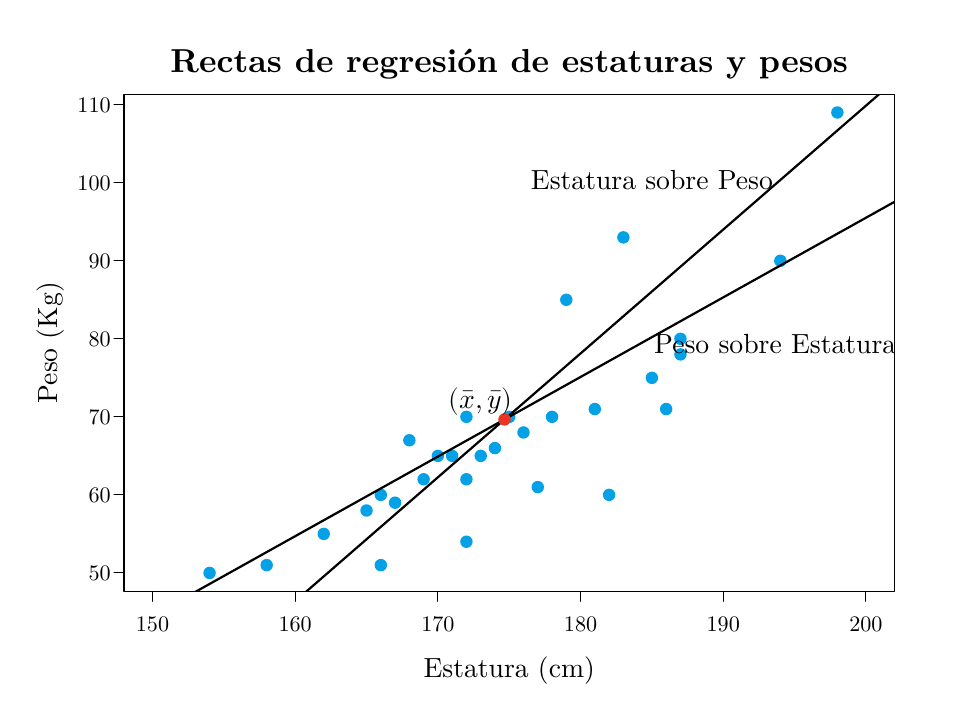
\begin{tikzpicture}[x=1pt,y=1pt]
\definecolor{fillColor}{RGB}{255,255,255}
\path[use as bounding box,fill=fillColor,fill opacity=0.00] (0,0) rectangle (325.21,238.49);
\begin{scope}
\path[clip] ( 34.80, 34.80) rectangle (313.21,214.49);
\definecolor{fillColor}{RGB}{5,161,230}

\path[fill=fillColor] (194.63,140.16) circle (  2.25);

\path[fill=fillColor] (163.70, 83.76) circle (  2.25);

\path[fill=fillColor] (204.94,100.68) circle (  2.25);

\path[fill=fillColor] (148.23, 83.76) circle (  2.25);

\path[fill=fillColor] ( 86.36, 44.28) circle (  2.25);

\path[fill=fillColor] (168.85, 86.58) circle (  2.25);

\path[fill=fillColor] (158.54, 75.30) circle (  2.25);

\path[fill=fillColor] (127.61, 69.66) circle (  2.25);

\path[fill=fillColor] (271.97,154.26) circle (  2.25);

\path[fill=fillColor] (225.57,111.96) circle (  2.25);

\path[fill=fillColor] (106.98, 55.56) circle (  2.25);

\path[fill=fillColor] (235.88,120.42) circle (  2.25);

\path[fill=fillColor] (292.59,207.84) circle (  2.25);

\path[fill=fillColor] (184.32, 72.48) circle (  2.25);

\path[fill=fillColor] (189.48, 97.86) circle (  2.25);

\path[fill=fillColor] (122.45, 64.02) circle (  2.25);

\path[fill=fillColor] ( 65.73, 41.46) circle (  2.25);

\path[fill=fillColor] (215.25,162.72) circle (  2.25);

\path[fill=fillColor] (127.61, 44.28) circle (  2.25);

\path[fill=fillColor] (153.38, 83.76) circle (  2.25);

\path[fill=fillColor] (174.01, 97.86) circle (  2.25);

\path[fill=fillColor] (210.10, 69.66) circle (  2.25);

\path[fill=fillColor] (132.76, 66.84) circle (  2.25);

\path[fill=fillColor] (143.07, 75.30) circle (  2.25);

\path[fill=fillColor] (158.54, 97.86) circle (  2.25);

\path[fill=fillColor] (230.72,100.68) circle (  2.25);

\path[fill=fillColor] (158.54, 52.74) circle (  2.25);

\path[fill=fillColor] (179.16, 92.22) circle (  2.25);

\path[fill=fillColor] (137.92, 89.40) circle (  2.25);

\path[fill=fillColor] (235.88,126.06) circle (  2.25);
\end{scope}
\begin{scope}
\path[clip] (  0.00,  0.00) rectangle (325.21,238.49);
\definecolor{drawColor}{RGB}{0,0,0}

\path[draw=drawColor,line width= 0.4pt,line join=round,line cap=round] ( 45.11, 34.80) -- (302.90, 34.80);

\path[draw=drawColor,line width= 0.4pt,line join=round,line cap=round] ( 45.11, 34.80) -- ( 45.11, 31.21);

\path[draw=drawColor,line width= 0.4pt,line join=round,line cap=round] ( 96.67, 34.80) -- ( 96.67, 31.21);

\path[draw=drawColor,line width= 0.4pt,line join=round,line cap=round] (148.23, 34.80) -- (148.23, 31.21);

\path[draw=drawColor,line width= 0.4pt,line join=round,line cap=round] (199.79, 34.80) -- (199.79, 31.21);

\path[draw=drawColor,line width= 0.4pt,line join=round,line cap=round] (251.34, 34.80) -- (251.34, 31.21);

\path[draw=drawColor,line width= 0.4pt,line join=round,line cap=round] (302.90, 34.80) -- (302.90, 31.21);

\node[text=drawColor,anchor=base,inner sep=0pt, outer sep=0pt, scale=  0.80] at ( 45.11, 20.40) {150};

\node[text=drawColor,anchor=base,inner sep=0pt, outer sep=0pt, scale=  0.80] at ( 96.67, 20.40) {160};

\node[text=drawColor,anchor=base,inner sep=0pt, outer sep=0pt, scale=  0.80] at (148.23, 20.40) {170};

\node[text=drawColor,anchor=base,inner sep=0pt, outer sep=0pt, scale=  0.80] at (199.79, 20.40) {180};

\node[text=drawColor,anchor=base,inner sep=0pt, outer sep=0pt, scale=  0.80] at (251.34, 20.40) {190};

\node[text=drawColor,anchor=base,inner sep=0pt, outer sep=0pt, scale=  0.80] at (302.90, 20.40) {200};

\path[draw=drawColor,line width= 0.4pt,line join=round,line cap=round] ( 34.80, 41.46) -- ( 34.80,210.66);

\path[draw=drawColor,line width= 0.4pt,line join=round,line cap=round] ( 34.80, 41.46) -- ( 31.21, 41.46);

\path[draw=drawColor,line width= 0.4pt,line join=round,line cap=round] ( 34.80, 69.66) -- ( 31.21, 69.66);

\path[draw=drawColor,line width= 0.4pt,line join=round,line cap=round] ( 34.80, 97.86) -- ( 31.21, 97.86);

\path[draw=drawColor,line width= 0.4pt,line join=round,line cap=round] ( 34.80,126.06) -- ( 31.21,126.06);

\path[draw=drawColor,line width= 0.4pt,line join=round,line cap=round] ( 34.80,154.26) -- ( 31.21,154.26);

\path[draw=drawColor,line width= 0.4pt,line join=round,line cap=round] ( 34.80,182.46) -- ( 31.21,182.46);

\path[draw=drawColor,line width= 0.4pt,line join=round,line cap=round] ( 34.80,210.66) -- ( 31.21,210.66);

\node[text=drawColor,anchor=base east,inner sep=0pt, outer sep=0pt, scale=  0.80] at ( 30.00, 38.70) {50};

\node[text=drawColor,anchor=base east,inner sep=0pt, outer sep=0pt, scale=  0.80] at ( 30.00, 66.90) {60};

\node[text=drawColor,anchor=base east,inner sep=0pt, outer sep=0pt, scale=  0.80] at ( 30.00, 95.10) {70};

\node[text=drawColor,anchor=base east,inner sep=0pt, outer sep=0pt, scale=  0.80] at ( 30.00,123.30) {80};

\node[text=drawColor,anchor=base east,inner sep=0pt, outer sep=0pt, scale=  0.80] at ( 30.00,151.50) {90};

\node[text=drawColor,anchor=base east,inner sep=0pt, outer sep=0pt, scale=  0.80] at ( 30.00,179.70) {100};

\node[text=drawColor,anchor=base east,inner sep=0pt, outer sep=0pt, scale=  0.80] at ( 30.00,207.90) {110};

\path[draw=drawColor,line width= 0.4pt,line join=round,line cap=round] ( 34.80, 34.80) --
	(313.21, 34.80) --
	(313.21,214.49) --
	( 34.80,214.49) --
	( 34.80, 34.80);
\end{scope}
\begin{scope}
\path[clip] (  0.00,  0.00) rectangle (325.21,238.49);
\definecolor{drawColor}{RGB}{0,0,0}

\node[text=drawColor,anchor=base,inner sep=0pt, outer sep=0pt, scale=  1.20] at (174.01,222.30) {\bfseries Rectas de regresión de estaturas y pesos};

\node[text=drawColor,anchor=base,inner sep=0pt, outer sep=0pt, scale=  1.00] at (174.01,  3.60) {Estatura (cm)};

\node[text=drawColor,rotate= 90.00,anchor=base,inner sep=0pt, outer sep=0pt, scale=  1.00] at ( 10.80,124.65) {Peso (Kg)};
\end{scope}
\begin{scope}
\path[clip] ( 34.80, 34.80) rectangle (313.21,214.49);
\definecolor{drawColor}{RGB}{0,0,0}

\path[draw=drawColor,line width= 0.8pt,line join=round,line cap=round] ( 34.80, 20.22) -- (313.21,175.55);

\path[draw=drawColor,line width= 0.8pt,line join=round,line cap=round] ( 60.68,  0.00) -- (313.21,219.25);
\definecolor{fillColor}{RGB}{238,50,36}

\path[fill=fillColor] (172.31, 96.92) circle (  2.25);

\node[text=drawColor,anchor=base,inner sep=0pt, outer sep=0pt, scale=  1.00] at (163.70,101.00) {$(\bar x, \bar y)$};

\node[text=drawColor,anchor=base,inner sep=0pt, outer sep=0pt, scale=  1.00] at (270.12,120.58) {Peso sobre Estatura};

\node[text=drawColor,anchor=base,inner sep=0pt, outer sep=0pt, scale=  1.00] at (225.57,179.98) {Estatura sobre Peso};
\end{scope}
\end{tikzpicture}
}}
\mode<presentation>{\resizebox{0.9\textwidth}{!}{% Created by tikzDevice version 0.10.1 on 2016-02-27 13:06:07
% !TEX encoding = UTF-8 Unicode
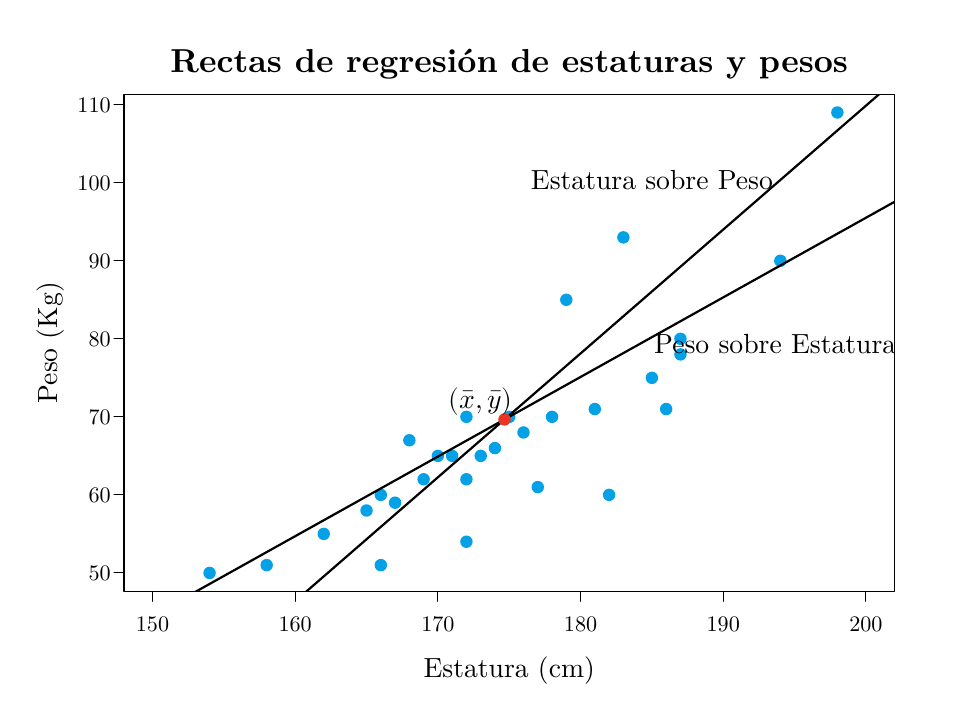
\begin{tikzpicture}[x=1pt,y=1pt]
\definecolor{fillColor}{RGB}{255,255,255}
\path[use as bounding box,fill=fillColor,fill opacity=0.00] (0,0) rectangle (325.21,238.49);
\begin{scope}
\path[clip] ( 34.80, 34.80) rectangle (313.21,214.49);
\definecolor{fillColor}{RGB}{5,161,230}

\path[fill=fillColor] (194.63,140.16) circle (  2.25);

\path[fill=fillColor] (163.70, 83.76) circle (  2.25);

\path[fill=fillColor] (204.94,100.68) circle (  2.25);

\path[fill=fillColor] (148.23, 83.76) circle (  2.25);

\path[fill=fillColor] ( 86.36, 44.28) circle (  2.25);

\path[fill=fillColor] (168.85, 86.58) circle (  2.25);

\path[fill=fillColor] (158.54, 75.30) circle (  2.25);

\path[fill=fillColor] (127.61, 69.66) circle (  2.25);

\path[fill=fillColor] (271.97,154.26) circle (  2.25);

\path[fill=fillColor] (225.57,111.96) circle (  2.25);

\path[fill=fillColor] (106.98, 55.56) circle (  2.25);

\path[fill=fillColor] (235.88,120.42) circle (  2.25);

\path[fill=fillColor] (292.59,207.84) circle (  2.25);

\path[fill=fillColor] (184.32, 72.48) circle (  2.25);

\path[fill=fillColor] (189.48, 97.86) circle (  2.25);

\path[fill=fillColor] (122.45, 64.02) circle (  2.25);

\path[fill=fillColor] ( 65.73, 41.46) circle (  2.25);

\path[fill=fillColor] (215.25,162.72) circle (  2.25);

\path[fill=fillColor] (127.61, 44.28) circle (  2.25);

\path[fill=fillColor] (153.38, 83.76) circle (  2.25);

\path[fill=fillColor] (174.01, 97.86) circle (  2.25);

\path[fill=fillColor] (210.10, 69.66) circle (  2.25);

\path[fill=fillColor] (132.76, 66.84) circle (  2.25);

\path[fill=fillColor] (143.07, 75.30) circle (  2.25);

\path[fill=fillColor] (158.54, 97.86) circle (  2.25);

\path[fill=fillColor] (230.72,100.68) circle (  2.25);

\path[fill=fillColor] (158.54, 52.74) circle (  2.25);

\path[fill=fillColor] (179.16, 92.22) circle (  2.25);

\path[fill=fillColor] (137.92, 89.40) circle (  2.25);

\path[fill=fillColor] (235.88,126.06) circle (  2.25);
\end{scope}
\begin{scope}
\path[clip] (  0.00,  0.00) rectangle (325.21,238.49);
\definecolor{drawColor}{RGB}{0,0,0}

\path[draw=drawColor,line width= 0.4pt,line join=round,line cap=round] ( 45.11, 34.80) -- (302.90, 34.80);

\path[draw=drawColor,line width= 0.4pt,line join=round,line cap=round] ( 45.11, 34.80) -- ( 45.11, 31.21);

\path[draw=drawColor,line width= 0.4pt,line join=round,line cap=round] ( 96.67, 34.80) -- ( 96.67, 31.21);

\path[draw=drawColor,line width= 0.4pt,line join=round,line cap=round] (148.23, 34.80) -- (148.23, 31.21);

\path[draw=drawColor,line width= 0.4pt,line join=round,line cap=round] (199.79, 34.80) -- (199.79, 31.21);

\path[draw=drawColor,line width= 0.4pt,line join=round,line cap=round] (251.34, 34.80) -- (251.34, 31.21);

\path[draw=drawColor,line width= 0.4pt,line join=round,line cap=round] (302.90, 34.80) -- (302.90, 31.21);

\node[text=drawColor,anchor=base,inner sep=0pt, outer sep=0pt, scale=  0.80] at ( 45.11, 20.40) {150};

\node[text=drawColor,anchor=base,inner sep=0pt, outer sep=0pt, scale=  0.80] at ( 96.67, 20.40) {160};

\node[text=drawColor,anchor=base,inner sep=0pt, outer sep=0pt, scale=  0.80] at (148.23, 20.40) {170};

\node[text=drawColor,anchor=base,inner sep=0pt, outer sep=0pt, scale=  0.80] at (199.79, 20.40) {180};

\node[text=drawColor,anchor=base,inner sep=0pt, outer sep=0pt, scale=  0.80] at (251.34, 20.40) {190};

\node[text=drawColor,anchor=base,inner sep=0pt, outer sep=0pt, scale=  0.80] at (302.90, 20.40) {200};

\path[draw=drawColor,line width= 0.4pt,line join=round,line cap=round] ( 34.80, 41.46) -- ( 34.80,210.66);

\path[draw=drawColor,line width= 0.4pt,line join=round,line cap=round] ( 34.80, 41.46) -- ( 31.21, 41.46);

\path[draw=drawColor,line width= 0.4pt,line join=round,line cap=round] ( 34.80, 69.66) -- ( 31.21, 69.66);

\path[draw=drawColor,line width= 0.4pt,line join=round,line cap=round] ( 34.80, 97.86) -- ( 31.21, 97.86);

\path[draw=drawColor,line width= 0.4pt,line join=round,line cap=round] ( 34.80,126.06) -- ( 31.21,126.06);

\path[draw=drawColor,line width= 0.4pt,line join=round,line cap=round] ( 34.80,154.26) -- ( 31.21,154.26);

\path[draw=drawColor,line width= 0.4pt,line join=round,line cap=round] ( 34.80,182.46) -- ( 31.21,182.46);

\path[draw=drawColor,line width= 0.4pt,line join=round,line cap=round] ( 34.80,210.66) -- ( 31.21,210.66);

\node[text=drawColor,anchor=base east,inner sep=0pt, outer sep=0pt, scale=  0.80] at ( 30.00, 38.70) {50};

\node[text=drawColor,anchor=base east,inner sep=0pt, outer sep=0pt, scale=  0.80] at ( 30.00, 66.90) {60};

\node[text=drawColor,anchor=base east,inner sep=0pt, outer sep=0pt, scale=  0.80] at ( 30.00, 95.10) {70};

\node[text=drawColor,anchor=base east,inner sep=0pt, outer sep=0pt, scale=  0.80] at ( 30.00,123.30) {80};

\node[text=drawColor,anchor=base east,inner sep=0pt, outer sep=0pt, scale=  0.80] at ( 30.00,151.50) {90};

\node[text=drawColor,anchor=base east,inner sep=0pt, outer sep=0pt, scale=  0.80] at ( 30.00,179.70) {100};

\node[text=drawColor,anchor=base east,inner sep=0pt, outer sep=0pt, scale=  0.80] at ( 30.00,207.90) {110};

\path[draw=drawColor,line width= 0.4pt,line join=round,line cap=round] ( 34.80, 34.80) --
	(313.21, 34.80) --
	(313.21,214.49) --
	( 34.80,214.49) --
	( 34.80, 34.80);
\end{scope}
\begin{scope}
\path[clip] (  0.00,  0.00) rectangle (325.21,238.49);
\definecolor{drawColor}{RGB}{0,0,0}

\node[text=drawColor,anchor=base,inner sep=0pt, outer sep=0pt, scale=  1.20] at (174.01,222.30) {\bfseries Rectas de regresión de estaturas y pesos};

\node[text=drawColor,anchor=base,inner sep=0pt, outer sep=0pt, scale=  1.00] at (174.01,  3.60) {Estatura (cm)};

\node[text=drawColor,rotate= 90.00,anchor=base,inner sep=0pt, outer sep=0pt, scale=  1.00] at ( 10.80,124.65) {Peso (Kg)};
\end{scope}
\begin{scope}
\path[clip] ( 34.80, 34.80) rectangle (313.21,214.49);
\definecolor{drawColor}{RGB}{0,0,0}

\path[draw=drawColor,line width= 0.8pt,line join=round,line cap=round] ( 34.80, 20.22) -- (313.21,175.55);

\path[draw=drawColor,line width= 0.8pt,line join=round,line cap=round] ( 60.68,  0.00) -- (313.21,219.25);
\definecolor{fillColor}{RGB}{238,50,36}

\path[fill=fillColor] (172.31, 96.92) circle (  2.25);

\node[text=drawColor,anchor=base,inner sep=0pt, outer sep=0pt, scale=  1.00] at (163.70,101.00) {$(\bar x, \bar y)$};

\node[text=drawColor,anchor=base,inner sep=0pt, outer sep=0pt, scale=  1.00] at (270.12,120.58) {Peso sobre Estatura};

\node[text=drawColor,anchor=base,inner sep=0pt, outer sep=0pt, scale=  1.00] at (225.57,179.98) {Estatura sobre Peso};
\end{scope}
\end{tikzpicture}
}}
\end{center}

\note{Si dibujamos ambas rectas, la del peso sobre la estatura y la de la estatura sobre el peso, podemos comprobar que se trata de rectas
distintas, ya que la primera hace mínimos los residuos del peso, y por tanto es la que debe utilizarse para predecir el peso en función de
la estatura, mientras que la segunda es la que hace mínimos los residuos de la estatura, y por tanto debe utilizarse para predecir la
estatura en función del peso.

Además puede comprobarse que las rectas de regresión se cortan en el punto de medias, lo cual se deduce fácilmente de sus respectivas
ecuaciones.
}
\end{frame}


%---------------------------------------------------------------------slide----
\begin{frame}
\frametitle{Posición relativa de las rectas de regresión}
Habitualmente, las rectas de regresión $Y$ sobre $X$ y de $X$
sobre $Y$ no coinciden, pero siempre se cortan en el punto de medias $(\bar x,\bar y)$.

\begin{columns}
\begin{column}{0.48\textwidth}
Si entre las variables la relación lineal es perfecta, entonces ambas rectas coinciden ya que sus residuos son nulos.
\begin{center}
\tikzsetnextfilename{regresion/regresion_lineal_perfecta}
\mode<article>{\resizebox{0.6\textwidth}{!}{% Created by tikzDevice version 0.10.1 on 2016-02-27 13:20:05
% !TEX encoding = UTF-8 Unicode
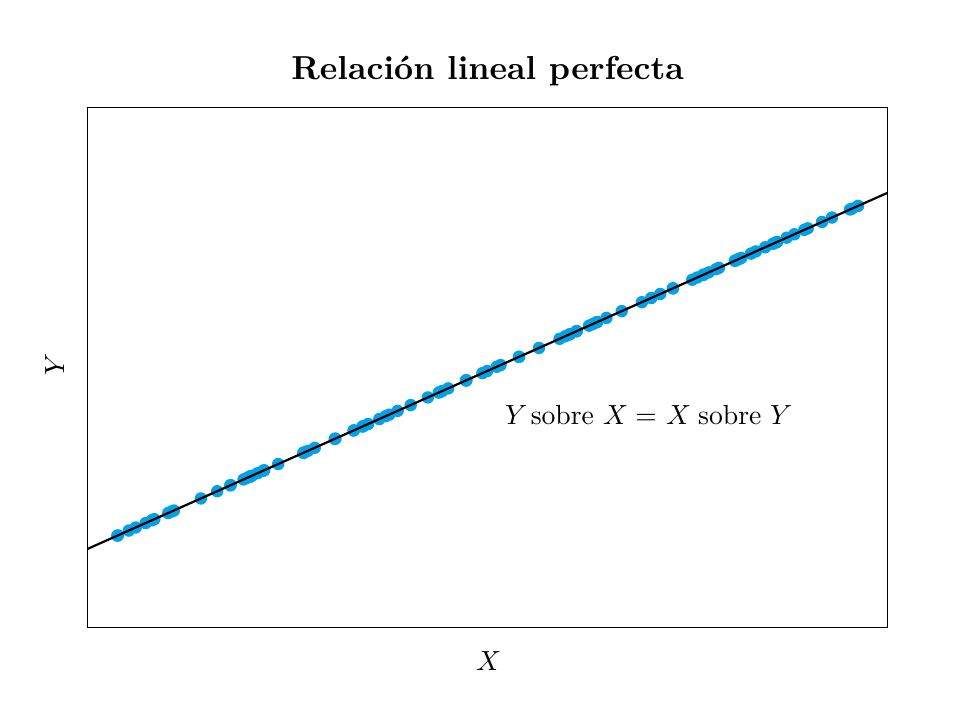
\begin{tikzpicture}[x=1pt,y=1pt]
\definecolor{fillColor}{RGB}{255,255,255}
\path[use as bounding box,fill=fillColor,fill opacity=0.00] (0,0) rectangle (325.21,238.49);
\begin{scope}
\path[clip] ( 21.68, 21.68) rectangle (310.76,209.58);
\definecolor{fillColor}{RGB}{5,161,230}

\path[fill=fillColor] (170.88,116.57) circle (  2.25);

\path[fill=fillColor] (177.53,119.53) circle (  2.25);

\path[fill=fillColor] ( 50.79, 63.12) circle (  2.25);

\path[fill=fillColor] ( 32.62, 55.02) circle (  2.25);

\path[fill=fillColor] (111.23, 90.02) circle (  2.25);

\path[fill=fillColor] (246.09,150.05) circle (  2.25);

\path[fill=fillColor] (266.49,159.13) circle (  2.25);

\path[fill=fillColor] (255.80,154.38) circle (  2.25);

\path[fill=fillColor] (148.53,106.62) circle (  2.25);

\path[fill=fillColor] ( 62.58, 68.36) circle (  2.25);

\path[fill=fillColor] ( 32.39, 54.92) circle (  2.25);

\path[fill=fillColor] ( 80.30, 76.25) circle (  2.25);

\path[fill=fillColor] (198.23,128.75) circle (  2.25);

\path[fill=fillColor] (228.57,142.26) circle (  2.25);

\path[fill=fillColor] (297.17,172.79) circle (  2.25);

\path[fill=fillColor] (101.29, 85.59) circle (  2.25);

\path[fill=fillColor] (184.76,122.75) circle (  2.25);

\path[fill=fillColor] (127.05, 97.06) circle (  2.25);

\path[fill=fillColor] (209.14,133.61) circle (  2.25);

\path[fill=fillColor] ( 99.88, 84.97) circle (  2.25);

\path[fill=fillColor] (277.02,163.82) circle (  2.25);

\path[fill=fillColor] ( 83.08, 77.49) circle (  2.25);

\path[fill=fillColor] (133.69,100.02) circle (  2.25);

\path[fill=fillColor] (123.00, 95.26) circle (  2.25);

\path[fill=fillColor] ( 52.00, 63.65) circle (  2.25);

\path[fill=fillColor] (202.86,130.81) circle (  2.25);

\path[fill=fillColor] (221.94,139.30) circle (  2.25);

\path[fill=fillColor] (255.50,154.24) circle (  2.25);

\path[fill=fillColor] (300.05,174.08) circle (  2.25);

\path[fill=fillColor] (164.33,113.66) circle (  2.25);

\path[fill=fillColor] (204.32,131.46) circle (  2.25);

\path[fill=fillColor] ( 45.77, 60.88) circle (  2.25);

\path[fill=fillColor] ( 80.54, 76.36) circle (  2.25);

\path[fill=fillColor] (257.83,155.28) circle (  2.25);

\path[fill=fillColor] ( 78.03, 75.24) circle (  2.25);

\path[fill=fillColor] (248.79,151.25) circle (  2.25);

\path[fill=fillColor] (270.78,161.04) circle (  2.25);

\path[fill=fillColor] (129.34, 98.08) circle (  2.25);

\path[fill=fillColor] (280.63,165.43) circle (  2.25);

\path[fill=fillColor] (195.95,127.73) circle (  2.25);

\path[fill=fillColor] (192.21,126.07) circle (  2.25);

\path[fill=fillColor] ( 52.84, 64.02) circle (  2.25);

\path[fill=fillColor] (151.97,108.15) circle (  2.25);

\path[fill=fillColor] (158.55,111.08) circle (  2.25);

\path[fill=fillColor] (256.72,154.79) circle (  2.25);

\path[fill=fillColor] (297.87,173.10) circle (  2.25);

\path[fill=fillColor] (263.10,157.63) circle (  2.25);

\path[fill=fillColor] ( 99.60, 84.84) circle (  2.25);

\path[fill=fillColor] ( 42.65, 59.49) circle (  2.25);

\path[fill=fillColor] (257.02,154.92) circle (  2.25);

\path[fill=fillColor] ( 79.42, 75.86) circle (  2.25);

\path[fill=fillColor] (225.33,140.81) circle (  2.25);

\path[fill=fillColor] ( 36.54, 56.77) circle (  2.25);

\path[fill=fillColor] ( 85.08, 78.38) circle (  2.25);

\path[fill=fillColor] (244.03,149.14) circle (  2.25);

\path[fill=fillColor] (158.39,111.01) circle (  2.25);

\path[fill=fillColor] ( 39.03, 57.88) circle (  2.25);

\path[fill=fillColor] (130.61, 98.64) circle (  2.25);

\path[fill=fillColor] (117.88, 92.98) circle (  2.25);

\path[fill=fillColor] (149.86,107.22) circle (  2.25);

\path[fill=fillColor] (261.37,156.85) circle (  2.25);

\path[fill=fillColor] (144.60,104.88) circle (  2.25);

\path[fill=fillColor] (205.84,132.14) circle (  2.25);

\path[fill=fillColor] (117.77, 92.93) circle (  2.25);

\path[fill=fillColor] (194.22,126.96) circle (  2.25);

\path[fill=fillColor] ( 68.49, 70.99) circle (  2.25);

\path[fill=fillColor] (198.43,128.84) circle (  2.25);

\path[fill=fillColor] (121.26, 94.49) circle (  2.25);

\path[fill=fillColor] (270.34,160.85) circle (  2.25);

\path[fill=fillColor] (233.15,144.29) circle (  2.25);

\path[fill=fillColor] ( 73.22, 73.10) circle (  2.25);

\path[fill=fillColor] (249.77,151.69) circle (  2.25);

\path[fill=fillColor] (103.73, 86.68) circle (  2.25);

\path[fill=fillColor] (120.96, 94.35) circle (  2.25);

\path[fill=fillColor] ( 80.43, 76.31) circle (  2.25);

\path[fill=fillColor] ( 85.48, 78.56) circle (  2.25);

\path[fill=fillColor] (214.66,136.06) circle (  2.25);

\path[fill=fillColor] ( 99.68, 84.88) circle (  2.25);

\path[fill=fillColor] (241.94,148.21) circle (  2.25);

\path[fill=fillColor] (281.87,165.98) circle (  2.25);

\path[fill=fillColor] ( 44.88, 60.48) circle (  2.25);

\path[fill=fillColor] (195.76,127.65) circle (  2.25);

\path[fill=fillColor] ( 81.05, 76.59) circle (  2.25);

\path[fill=fillColor] ( 90.53, 80.81) circle (  2.25);

\path[fill=fillColor] (290.62,169.88) circle (  2.25);

\path[fill=fillColor] (158.42,111.03) circle (  2.25);

\path[fill=fillColor] (177.57,119.55) circle (  2.25);

\path[fill=fillColor] (205.60,132.03) circle (  2.25);

\path[fill=fillColor] (110.95, 89.89) circle (  2.25);

\path[fill=fillColor] (138.40,102.11) circle (  2.25);

\path[fill=fillColor] ( 73.37, 73.17) circle (  2.25);

\path[fill=fillColor] (233.18,144.31) circle (  2.25);

\path[fill=fillColor] (240.15,147.41) circle (  2.25);

\path[fill=fillColor] (244.40,149.30) circle (  2.25);

\path[fill=fillColor] (149.31,106.97) circle (  2.25);

\path[fill=fillColor] (166.05,114.42) circle (  2.25);

\path[fill=fillColor] (274.27,162.60) circle (  2.25);

\path[fill=fillColor] (287.03,168.28) circle (  2.25);

\path[fill=fillColor] (169.50,115.96) circle (  2.25);

\path[fill=fillColor] (269.30,160.39) circle (  2.25);
\end{scope}
\begin{scope}
\path[clip] (  0.00,  0.00) rectangle (325.21,238.49);
\definecolor{drawColor}{RGB}{0,0,0}

\node[text=drawColor,anchor=base,inner sep=0pt, outer sep=0pt, scale=  1.20] at (166.22,219.84) {\bfseries Relación lineal perfecta};

\node[text=drawColor,anchor=base,inner sep=0pt, outer sep=0pt, scale=  1.00] at (166.22,  6.08) {$X$};

\node[text=drawColor,rotate= 90.00,anchor=base,inner sep=0pt, outer sep=0pt, scale=  1.00] at ( 13.28,115.63) {$Y$};
\end{scope}
\begin{scope}
\path[clip] (  0.00,  0.00) rectangle (325.21,238.49);
\definecolor{drawColor}{RGB}{0,0,0}

\path[draw=drawColor,line width= 0.4pt,line join=round,line cap=round] ( 21.68, 21.68) --
	(310.76, 21.68) --
	(310.76,209.58) --
	( 21.68,209.58) --
	( 21.68, 21.68);
\end{scope}
\begin{scope}
\path[clip] ( 21.68, 21.68) rectangle (310.76,209.58);
\definecolor{drawColor}{RGB}{0,0,0}

\path[draw=drawColor,line width= 0.8pt,line join=round,line cap=round] ( 21.68, 50.16) -- (310.76,178.84);

\node[text=drawColor,anchor=base,inner sep=0pt, outer sep=0pt, scale=  1.00] at (223.48, 94.97) {$Y$ sobre $X$ = $X$ sobre $Y$};
\end{scope}
\end{tikzpicture}
}}
\mode<presentation>{\resizebox{0.9\textwidth}{!}{% Created by tikzDevice version 0.10.1 on 2016-02-27 13:20:05
% !TEX encoding = UTF-8 Unicode
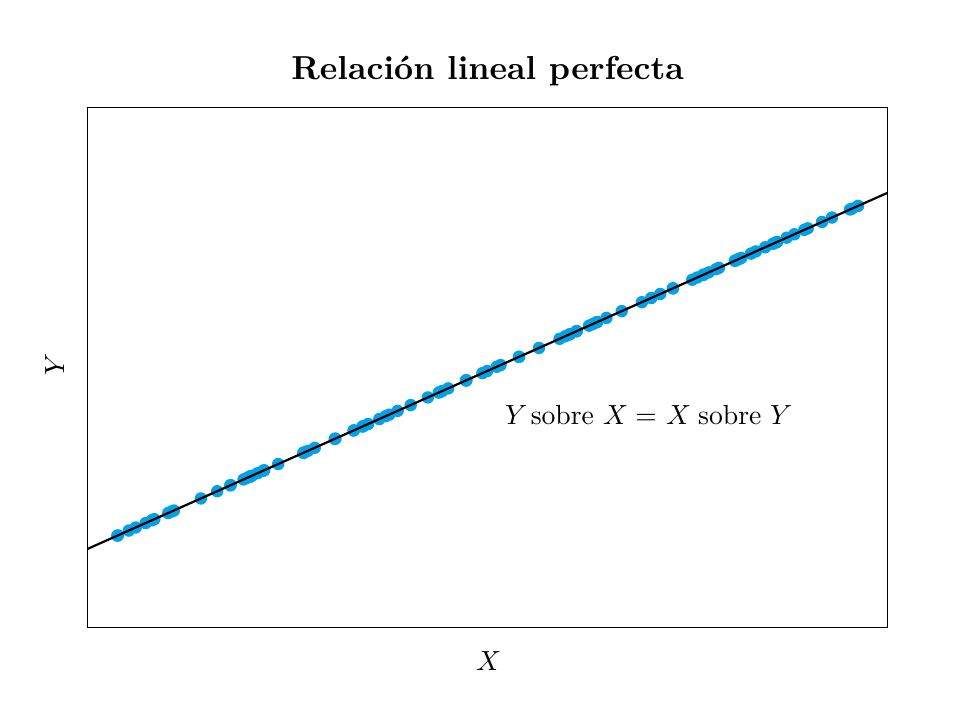
\begin{tikzpicture}[x=1pt,y=1pt]
\definecolor{fillColor}{RGB}{255,255,255}
\path[use as bounding box,fill=fillColor,fill opacity=0.00] (0,0) rectangle (325.21,238.49);
\begin{scope}
\path[clip] ( 21.68, 21.68) rectangle (310.76,209.58);
\definecolor{fillColor}{RGB}{5,161,230}

\path[fill=fillColor] (170.88,116.57) circle (  2.25);

\path[fill=fillColor] (177.53,119.53) circle (  2.25);

\path[fill=fillColor] ( 50.79, 63.12) circle (  2.25);

\path[fill=fillColor] ( 32.62, 55.02) circle (  2.25);

\path[fill=fillColor] (111.23, 90.02) circle (  2.25);

\path[fill=fillColor] (246.09,150.05) circle (  2.25);

\path[fill=fillColor] (266.49,159.13) circle (  2.25);

\path[fill=fillColor] (255.80,154.38) circle (  2.25);

\path[fill=fillColor] (148.53,106.62) circle (  2.25);

\path[fill=fillColor] ( 62.58, 68.36) circle (  2.25);

\path[fill=fillColor] ( 32.39, 54.92) circle (  2.25);

\path[fill=fillColor] ( 80.30, 76.25) circle (  2.25);

\path[fill=fillColor] (198.23,128.75) circle (  2.25);

\path[fill=fillColor] (228.57,142.26) circle (  2.25);

\path[fill=fillColor] (297.17,172.79) circle (  2.25);

\path[fill=fillColor] (101.29, 85.59) circle (  2.25);

\path[fill=fillColor] (184.76,122.75) circle (  2.25);

\path[fill=fillColor] (127.05, 97.06) circle (  2.25);

\path[fill=fillColor] (209.14,133.61) circle (  2.25);

\path[fill=fillColor] ( 99.88, 84.97) circle (  2.25);

\path[fill=fillColor] (277.02,163.82) circle (  2.25);

\path[fill=fillColor] ( 83.08, 77.49) circle (  2.25);

\path[fill=fillColor] (133.69,100.02) circle (  2.25);

\path[fill=fillColor] (123.00, 95.26) circle (  2.25);

\path[fill=fillColor] ( 52.00, 63.65) circle (  2.25);

\path[fill=fillColor] (202.86,130.81) circle (  2.25);

\path[fill=fillColor] (221.94,139.30) circle (  2.25);

\path[fill=fillColor] (255.50,154.24) circle (  2.25);

\path[fill=fillColor] (300.05,174.08) circle (  2.25);

\path[fill=fillColor] (164.33,113.66) circle (  2.25);

\path[fill=fillColor] (204.32,131.46) circle (  2.25);

\path[fill=fillColor] ( 45.77, 60.88) circle (  2.25);

\path[fill=fillColor] ( 80.54, 76.36) circle (  2.25);

\path[fill=fillColor] (257.83,155.28) circle (  2.25);

\path[fill=fillColor] ( 78.03, 75.24) circle (  2.25);

\path[fill=fillColor] (248.79,151.25) circle (  2.25);

\path[fill=fillColor] (270.78,161.04) circle (  2.25);

\path[fill=fillColor] (129.34, 98.08) circle (  2.25);

\path[fill=fillColor] (280.63,165.43) circle (  2.25);

\path[fill=fillColor] (195.95,127.73) circle (  2.25);

\path[fill=fillColor] (192.21,126.07) circle (  2.25);

\path[fill=fillColor] ( 52.84, 64.02) circle (  2.25);

\path[fill=fillColor] (151.97,108.15) circle (  2.25);

\path[fill=fillColor] (158.55,111.08) circle (  2.25);

\path[fill=fillColor] (256.72,154.79) circle (  2.25);

\path[fill=fillColor] (297.87,173.10) circle (  2.25);

\path[fill=fillColor] (263.10,157.63) circle (  2.25);

\path[fill=fillColor] ( 99.60, 84.84) circle (  2.25);

\path[fill=fillColor] ( 42.65, 59.49) circle (  2.25);

\path[fill=fillColor] (257.02,154.92) circle (  2.25);

\path[fill=fillColor] ( 79.42, 75.86) circle (  2.25);

\path[fill=fillColor] (225.33,140.81) circle (  2.25);

\path[fill=fillColor] ( 36.54, 56.77) circle (  2.25);

\path[fill=fillColor] ( 85.08, 78.38) circle (  2.25);

\path[fill=fillColor] (244.03,149.14) circle (  2.25);

\path[fill=fillColor] (158.39,111.01) circle (  2.25);

\path[fill=fillColor] ( 39.03, 57.88) circle (  2.25);

\path[fill=fillColor] (130.61, 98.64) circle (  2.25);

\path[fill=fillColor] (117.88, 92.98) circle (  2.25);

\path[fill=fillColor] (149.86,107.22) circle (  2.25);

\path[fill=fillColor] (261.37,156.85) circle (  2.25);

\path[fill=fillColor] (144.60,104.88) circle (  2.25);

\path[fill=fillColor] (205.84,132.14) circle (  2.25);

\path[fill=fillColor] (117.77, 92.93) circle (  2.25);

\path[fill=fillColor] (194.22,126.96) circle (  2.25);

\path[fill=fillColor] ( 68.49, 70.99) circle (  2.25);

\path[fill=fillColor] (198.43,128.84) circle (  2.25);

\path[fill=fillColor] (121.26, 94.49) circle (  2.25);

\path[fill=fillColor] (270.34,160.85) circle (  2.25);

\path[fill=fillColor] (233.15,144.29) circle (  2.25);

\path[fill=fillColor] ( 73.22, 73.10) circle (  2.25);

\path[fill=fillColor] (249.77,151.69) circle (  2.25);

\path[fill=fillColor] (103.73, 86.68) circle (  2.25);

\path[fill=fillColor] (120.96, 94.35) circle (  2.25);

\path[fill=fillColor] ( 80.43, 76.31) circle (  2.25);

\path[fill=fillColor] ( 85.48, 78.56) circle (  2.25);

\path[fill=fillColor] (214.66,136.06) circle (  2.25);

\path[fill=fillColor] ( 99.68, 84.88) circle (  2.25);

\path[fill=fillColor] (241.94,148.21) circle (  2.25);

\path[fill=fillColor] (281.87,165.98) circle (  2.25);

\path[fill=fillColor] ( 44.88, 60.48) circle (  2.25);

\path[fill=fillColor] (195.76,127.65) circle (  2.25);

\path[fill=fillColor] ( 81.05, 76.59) circle (  2.25);

\path[fill=fillColor] ( 90.53, 80.81) circle (  2.25);

\path[fill=fillColor] (290.62,169.88) circle (  2.25);

\path[fill=fillColor] (158.42,111.03) circle (  2.25);

\path[fill=fillColor] (177.57,119.55) circle (  2.25);

\path[fill=fillColor] (205.60,132.03) circle (  2.25);

\path[fill=fillColor] (110.95, 89.89) circle (  2.25);

\path[fill=fillColor] (138.40,102.11) circle (  2.25);

\path[fill=fillColor] ( 73.37, 73.17) circle (  2.25);

\path[fill=fillColor] (233.18,144.31) circle (  2.25);

\path[fill=fillColor] (240.15,147.41) circle (  2.25);

\path[fill=fillColor] (244.40,149.30) circle (  2.25);

\path[fill=fillColor] (149.31,106.97) circle (  2.25);

\path[fill=fillColor] (166.05,114.42) circle (  2.25);

\path[fill=fillColor] (274.27,162.60) circle (  2.25);

\path[fill=fillColor] (287.03,168.28) circle (  2.25);

\path[fill=fillColor] (169.50,115.96) circle (  2.25);

\path[fill=fillColor] (269.30,160.39) circle (  2.25);
\end{scope}
\begin{scope}
\path[clip] (  0.00,  0.00) rectangle (325.21,238.49);
\definecolor{drawColor}{RGB}{0,0,0}

\node[text=drawColor,anchor=base,inner sep=0pt, outer sep=0pt, scale=  1.20] at (166.22,219.84) {\bfseries Relación lineal perfecta};

\node[text=drawColor,anchor=base,inner sep=0pt, outer sep=0pt, scale=  1.00] at (166.22,  6.08) {$X$};

\node[text=drawColor,rotate= 90.00,anchor=base,inner sep=0pt, outer sep=0pt, scale=  1.00] at ( 13.28,115.63) {$Y$};
\end{scope}
\begin{scope}
\path[clip] (  0.00,  0.00) rectangle (325.21,238.49);
\definecolor{drawColor}{RGB}{0,0,0}

\path[draw=drawColor,line width= 0.4pt,line join=round,line cap=round] ( 21.68, 21.68) --
	(310.76, 21.68) --
	(310.76,209.58) --
	( 21.68,209.58) --
	( 21.68, 21.68);
\end{scope}
\begin{scope}
\path[clip] ( 21.68, 21.68) rectangle (310.76,209.58);
\definecolor{drawColor}{RGB}{0,0,0}

\path[draw=drawColor,line width= 0.8pt,line join=round,line cap=round] ( 21.68, 50.16) -- (310.76,178.84);

\node[text=drawColor,anchor=base,inner sep=0pt, outer sep=0pt, scale=  1.00] at (223.48, 94.97) {$Y$ sobre $X$ = $X$ sobre $Y$};
\end{scope}
\end{tikzpicture}
}}
\end{center}
\end{column}
\begin{column}{0.48\textwidth}
Si no hay relación lineal, entonces las ecuaciones de las rectas son\\
\qquad \qquad $y = \bar y$, \qquad $x = \bar x,$\\
y se cortan perpendicularmente  
\begin{center}
\tikzsetnextfilename{regresion/rectas_independencia_lineal}
\mode<article>{\resizebox{0.6\textwidth}{!}{%% Input file name: rectas_independencia_lineal.fig
%% FIG version: 3.2
%% Orientation: Landscape
%% Justification: Flush Left
%% Units: Inches
%% Paper size: A4
%% Magnification: 100.0
%% Resolution: 1200ppi
%% Include the following in the preamble:
%% \usepackage{textcomp}
%% End

\begin{pspicture}(7.06cm,3.29cm)(16.36cm,13.56cm)
\psset{unit=0.8cm}
%%
%% Depth: 2147483647
%%
\newrgbcolor{mycolor0}{1.00 0.50 0.31}\definecolor{mycolor0}{rgb}{1.00,0.50,0.31}
%%
%% Depth: 100
%%
\psset{linestyle=solid,linewidth=0.03175,linecolor=mycolor0}
\qdisk(16.63,9.96){0.1}
\qdisk(18.53,10.92){0.1}
\qdisk(13.60,12.64){0.1}
\qdisk(12.83,13.91){0.1}
\qdisk(16.21,6.16){0.1}
\qdisk(16.04,9.07){0.1}
\qdisk(17.89,6.74){0.1}
\qdisk(13.39,11.97){0.1}
\qdisk(13.66,9.79){0.1}
\qdisk(18.77,11.43){0.1}
\qdisk(18.79,10.20){0.1}
\qdisk(15.90,13.76){0.1}
\qdisk(16.33,11.13){0.1}
\qdisk(18.47,9.84){0.1}
\qdisk(11.42,6.20){0.1}
\qdisk(10.15,9.35){0.1}
\qdisk(15.48,12.85){0.1}
\qdisk(12.40,9.99){0.1}
\qdisk(13.81,13.59){0.1}
\qdisk(17.18,6.11){0.1}
\qdisk(17.94,8.41){0.1}
\qdisk(17.76,13.78){0.1}
\qdisk(13.97,8.58){0.1}
\qdisk(18.60,5.92){0.1}
\qdisk(10.92,14.58){0.1}
\qdisk(16.44,12.66){0.1}
\qdisk(18.74,14.83){0.1}
\qdisk(12.98,11.21){0.1}
\qdisk(10.70,8.89){0.1}
\qdisk(10.33,7.27){0.1}
\qdisk(17.96,11.10){0.1}
\qdisk(12.36,15.04){0.1}
\qdisk(17.98,13.34){0.1}
\qdisk(19.55,8.17){0.1}
\qdisk(10.25,6.88){0.1}
\qdisk(12.06,15.26){0.1}
\qdisk(15.21,8.56){0.1}
\qdisk(11.72,8.30){0.1}
\qdisk(12.25,10.12){0.1}
\qdisk(12.58,12.44){0.1}
\qdisk(11.91,12.42){0.1}
\qdisk(14.86,11.21){0.1}
\qdisk(13.75,13.21){0.1}
\qdisk(15.09,15.10){0.1}
\qdisk(12.35,7.22){0.1}
\qdisk(10.73,9.81){0.1}
\qdisk(10.43,14.15){0.1}
\qdisk(11.32,8.59){0.1}
\qdisk(16.15,12.81){0.1}
\qdisk(19.51,7.91){0.1}
\qdisk(11.44,13.64){0.1}
\qdisk(11.21,12.44){0.1}
\qdisk(18.86,6.46){0.1}
\qdisk(10.31,10.08){0.1}
\qdisk(14.02,13.31){0.1}
\qdisk(17.26,8.80){0.1}
\qdisk(13.32,8.87){0.1}
\qdisk(11.63,6.47){0.1}
\qdisk(18.64,9.07){0.1}
\qdisk(11.00,7.62){0.1}
\qdisk(11.52,5.85){0.1}
\qdisk(15.30,7.81){0.1}
\qdisk(10.55,6.39){0.1}
\qdisk(17.38,12.21){0.1}
\qdisk(15.61,13.11){0.1}
\qdisk(10.75,12.83){0.1}
\qdisk(12.50,8.51){0.1}
\qdisk(17.62,13.47){0.1}
\qdisk(12.53,11.83){0.1}
\qdisk(12.42,6.73){0.1}
\qdisk(16.71,12.34){0.1}
\qdisk(13.96,13.40){0.1}
\qdisk(12.70,14.84){0.1}
\qdisk(18.84,8.00){0.1}
\qdisk(10.69,9.75){0.1}
\qdisk(14.34,8.62){0.1}
\qdisk(18.00,11.21){0.1}
\qdisk(14.23,6.39){0.1}
\qdisk(11.13,8.85){0.1}
\qdisk(16.74,7.02){0.1}
\qdisk(13.69,13.22){0.1}
\qdisk(11.43,10.96){0.1}
\qdisk(14.30,6.05){0.1}
\qdisk(18.77,13.78){0.1}
\qdisk(12.15,6.08){0.1}
\qdisk(10.41,12.01){0.1}
\qdisk(16.28,10.93){0.1}
\qdisk(19.51,12.10){0.1}
\qdisk(10.27,7.83){0.1}
\qdisk(17.47,8.75){0.1}
\qdisk(15.26,9.19){0.1}
\qdisk(17.82,6.24){0.1}
\qdisk(16.99,15.21){0.1}
\qdisk(10.35,7.39){0.1}
\qdisk(15.29,8.17){0.1}
\qdisk(19.06,6.05){0.1}
\qdisk(17.96,8.48){0.1}
\qdisk(15.95,8.06){0.1}
\qdisk(15.13,6.57){0.1}
\qdisk(14.13,10.01){0.1}
\rput(14.85,16.12){Sin relación lineal}
\rput[l](14.71,4.63){$X$}
\rput[l]{90}(9.35,10.42){$Y$}
\psset{linecolor=black,fillstyle=none}
\psline(9.77,5.48)(19.93,5.48)(19.93,15.64)(9.77,15.64)(9.77,5.48)
\psset{linewidth=0.0635}
\psline(9.77,10.16)(19.93,10.16)
\psline(14.57,5.48)(14.57,15.64)
\rput[l](14.72,6.85){$X$ sobre $Y$}
\rput[l](17.82,9.57){$Y$ sobre $X$}
\end{pspicture}
%% End
}}
\mode<presentation>{\resizebox{0.9\textwidth}{!}{%% Input file name: rectas_independencia_lineal.fig
%% FIG version: 3.2
%% Orientation: Landscape
%% Justification: Flush Left
%% Units: Inches
%% Paper size: A4
%% Magnification: 100.0
%% Resolution: 1200ppi
%% Include the following in the preamble:
%% \usepackage{textcomp}
%% End

\begin{pspicture}(7.06cm,3.29cm)(16.36cm,13.56cm)
\psset{unit=0.8cm}
%%
%% Depth: 2147483647
%%
\newrgbcolor{mycolor0}{1.00 0.50 0.31}\definecolor{mycolor0}{rgb}{1.00,0.50,0.31}
%%
%% Depth: 100
%%
\psset{linestyle=solid,linewidth=0.03175,linecolor=mycolor0}
\qdisk(16.63,9.96){0.1}
\qdisk(18.53,10.92){0.1}
\qdisk(13.60,12.64){0.1}
\qdisk(12.83,13.91){0.1}
\qdisk(16.21,6.16){0.1}
\qdisk(16.04,9.07){0.1}
\qdisk(17.89,6.74){0.1}
\qdisk(13.39,11.97){0.1}
\qdisk(13.66,9.79){0.1}
\qdisk(18.77,11.43){0.1}
\qdisk(18.79,10.20){0.1}
\qdisk(15.90,13.76){0.1}
\qdisk(16.33,11.13){0.1}
\qdisk(18.47,9.84){0.1}
\qdisk(11.42,6.20){0.1}
\qdisk(10.15,9.35){0.1}
\qdisk(15.48,12.85){0.1}
\qdisk(12.40,9.99){0.1}
\qdisk(13.81,13.59){0.1}
\qdisk(17.18,6.11){0.1}
\qdisk(17.94,8.41){0.1}
\qdisk(17.76,13.78){0.1}
\qdisk(13.97,8.58){0.1}
\qdisk(18.60,5.92){0.1}
\qdisk(10.92,14.58){0.1}
\qdisk(16.44,12.66){0.1}
\qdisk(18.74,14.83){0.1}
\qdisk(12.98,11.21){0.1}
\qdisk(10.70,8.89){0.1}
\qdisk(10.33,7.27){0.1}
\qdisk(17.96,11.10){0.1}
\qdisk(12.36,15.04){0.1}
\qdisk(17.98,13.34){0.1}
\qdisk(19.55,8.17){0.1}
\qdisk(10.25,6.88){0.1}
\qdisk(12.06,15.26){0.1}
\qdisk(15.21,8.56){0.1}
\qdisk(11.72,8.30){0.1}
\qdisk(12.25,10.12){0.1}
\qdisk(12.58,12.44){0.1}
\qdisk(11.91,12.42){0.1}
\qdisk(14.86,11.21){0.1}
\qdisk(13.75,13.21){0.1}
\qdisk(15.09,15.10){0.1}
\qdisk(12.35,7.22){0.1}
\qdisk(10.73,9.81){0.1}
\qdisk(10.43,14.15){0.1}
\qdisk(11.32,8.59){0.1}
\qdisk(16.15,12.81){0.1}
\qdisk(19.51,7.91){0.1}
\qdisk(11.44,13.64){0.1}
\qdisk(11.21,12.44){0.1}
\qdisk(18.86,6.46){0.1}
\qdisk(10.31,10.08){0.1}
\qdisk(14.02,13.31){0.1}
\qdisk(17.26,8.80){0.1}
\qdisk(13.32,8.87){0.1}
\qdisk(11.63,6.47){0.1}
\qdisk(18.64,9.07){0.1}
\qdisk(11.00,7.62){0.1}
\qdisk(11.52,5.85){0.1}
\qdisk(15.30,7.81){0.1}
\qdisk(10.55,6.39){0.1}
\qdisk(17.38,12.21){0.1}
\qdisk(15.61,13.11){0.1}
\qdisk(10.75,12.83){0.1}
\qdisk(12.50,8.51){0.1}
\qdisk(17.62,13.47){0.1}
\qdisk(12.53,11.83){0.1}
\qdisk(12.42,6.73){0.1}
\qdisk(16.71,12.34){0.1}
\qdisk(13.96,13.40){0.1}
\qdisk(12.70,14.84){0.1}
\qdisk(18.84,8.00){0.1}
\qdisk(10.69,9.75){0.1}
\qdisk(14.34,8.62){0.1}
\qdisk(18.00,11.21){0.1}
\qdisk(14.23,6.39){0.1}
\qdisk(11.13,8.85){0.1}
\qdisk(16.74,7.02){0.1}
\qdisk(13.69,13.22){0.1}
\qdisk(11.43,10.96){0.1}
\qdisk(14.30,6.05){0.1}
\qdisk(18.77,13.78){0.1}
\qdisk(12.15,6.08){0.1}
\qdisk(10.41,12.01){0.1}
\qdisk(16.28,10.93){0.1}
\qdisk(19.51,12.10){0.1}
\qdisk(10.27,7.83){0.1}
\qdisk(17.47,8.75){0.1}
\qdisk(15.26,9.19){0.1}
\qdisk(17.82,6.24){0.1}
\qdisk(16.99,15.21){0.1}
\qdisk(10.35,7.39){0.1}
\qdisk(15.29,8.17){0.1}
\qdisk(19.06,6.05){0.1}
\qdisk(17.96,8.48){0.1}
\qdisk(15.95,8.06){0.1}
\qdisk(15.13,6.57){0.1}
\qdisk(14.13,10.01){0.1}
\rput(14.85,16.12){Sin relación lineal}
\rput[l](14.71,4.63){$X$}
\rput[l]{90}(9.35,10.42){$Y$}
\psset{linecolor=black,fillstyle=none}
\psline(9.77,5.48)(19.93,5.48)(19.93,15.64)(9.77,15.64)(9.77,5.48)
\psset{linewidth=0.0635}
\psline(9.77,10.16)(19.93,10.16)
\psline(14.57,5.48)(14.57,15.64)
\rput[l](14.72,6.85){$X$ sobre $Y$}
\rput[l](17.82,9.57){$Y$ sobre $X$}
\end{pspicture}
%% End
}}
\end{center}
\end{column}
\end{columns}

\note{La posición relativa de las rectas de regresión depende del grado de relación lineal entre las variables. 

Si la relación lineal entre las variables es perfecta, entonces los puntos de la nube de puntos estarán perfectamente alineados y la
recta de regresión de $Y$ sobre $X$ y de $X$ sobre $Y$ coincidirán en la recta que pasa por todos los puntos ya que para esta recta tanto
los residuos en $Y$ como los residuos en $X$ serán nulos.

Mientras que si no hay relación lineal entre las variables, entonces la covarianza será nula y la ecuación de las rectas será constante, $y
= \bar y$, para la recta de $Y$ sobre $X$, y $x = \bar x$ para la de $X$ sobre $Y$, de manera que las rectas se cortarán perpendicularmente en el punto
de medias.

Así pues, cuanto menor sea el ángulo con que se cortan las rectas, mayor será la dependencia lineal entre las variables.
}
\end{frame}


%---------------------------------------------------------------------slide----
\begin{frame}
\frametitle{Coeficiente de regresión}
El parámetro más importante de una recta de regresión es su pendiente.

\begin{definicion}[Coeficiente de regresión $b_{yx}$]
Dada una variable bidimensional $(X,Y)$, el \emph{coeficiente de regresión} de la recta de regresión de $Y$ sobre $X$ es su pendiente,
\[
b_{yx} = \frac{s_{xy}}{s_x^2} 
\]
\end{definicion}

El coeficiente de regresión siempre tiene el mismo signo que la covarianza.

Refleja el crecimiento de la variable dependiente en relación a la independiente según la recta de regresión. 
En concreto da el número de unidades que aumenta o disminuye la variable dependiente por cada unidad que aumenta la variable independiente.
\note{En la ecuación de la recta de regresión de $Y$ sobre $X$, la parte más importante es la pendiente que se conoce como coeficiente de
regresión de $Y$ sobre $X$ y vale $b_{yx} = \frac{s_{xy}}{s_x^2}$.

El coeficiente de regresión siempre tiene el mismo signo que la covarianza. 

Refleja el crecimiento de la variable dependiente en relación a la independiente según la recta de regresión. En concreto da el número de unidades que aumenta o disminuye la variable dependiente por cada unidad que aumenta la variable independiente.}
\end{frame}

%---------------------------------------------------------------------slide----
\begin{frame}
\frametitle{Regression coefficient}
\framesubtitle{Example of heights and weights}

En el ejemplo de las estaturas y los pesos, la recta de regresión del peso sobre la estatura era
\[
y=-108.49 +1.02 x,
\]
de manera que el coeficiente de regresión del peso sobre la estatura es 
\[
b_{yx}= 1.02 \mbox{Kg/cm.}
\]
Esto significa que, según la recta de regresión del peso sobre la estatura, por cada cm más de estatura, la persona pesará $1.02$ Kg más.

\begin{center}
\tikzsetnextfilename{regresion/interpretacion_pendiente}
% Author: Alfredo Sánchez Alberca (asalber@ceu.es)
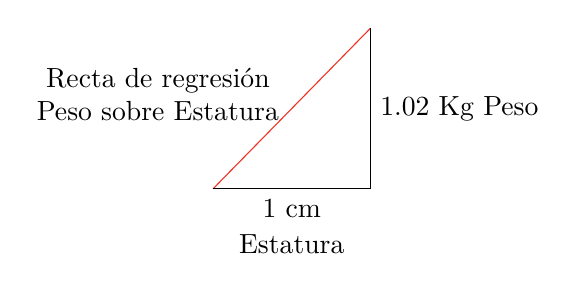
\begin{tikzpicture}
\draw[color=color2] (0,0) -- (2,2.04);
\draw (0,0) -- (2,0) -- (2,2.04);
\node[align=center] at (-0.7,1.2) {Recta de regresión\\ Peso sobre Estatura};
\node[anchor=north] at (1,0) {1 cm};
\node at (1,-0.7){Estatura};
\node[anchor=west] at (2,1.02) {1.02 Kg  Peso};
\end{tikzpicture}

\end{center}


\note{En el ejemplo de las estaturas y los pesos, el coeficiente de regresión del peso sobre la estatura es $b_{yx}= 1.02$ Kg/cm, lo que indica
que, según la recta de regresión del peso sobre la estatura, por cada cm más de estatura, la persona pesará $1.02$ Kg más.
}
\end{frame}


%---------------------------------------------------------------------slide----
\begin{frame}
\frametitle{Predicciones con las rectas de regresión}
\framesubtitle{Ejemplo con estaturas y pesos}
Las rectas de regresión, y en general cualquier modelo de regresión, suele utilizarse con fines predictivos. 

\begin{center}
\alert{\emph{¡Ojo! Para predecir una variable, esta siempre debe considerarse como dependiente en el modelo de regresión que se utilice.}}
\end{center}

Así, en el ejemplo de las estaturas y los pesos, si se quiere predecir el peso de una persona que mide 180 cm, se debe utilizar la recta de
regresión del peso sobre la estatura:
\[
y = 1.02 \cdot 180 -108.49 = 75.11 \mbox{ Kg}.
\] 
Y si se quiere predecir la estatura de una persona que pesa 79 Kg, se debe utilizar la recta de regresión de la estatura sobre el peso:
\[
x = 0.63\cdot 79+ 130.78 = 180.55 \mbox{ cm}. 
\]
\begin{center}
\emph{Ahora bien, ¿qué fiabilidad tienen estas predicciones?}
\end{center}

\note{Las rectas de regresión, y en general cualquier modelo de regresión, suele utilizarse con fines predictivos. 

Como hemos visto, dependiendo de si se toma $X$ o $Y$ como la variable dependiente, tendremos modelos de regresión, el de $Y$ sobre $X$ y
el de $X$ sobre $Y$, pero a la hora de hacer predicciones de una variable, siempre debe utilizarse el modelo en el que dicha variable sea la
variable dependiente, ya que ese será el modelo que haga mínimos los errores predictivos en dicha variable.

Por ejemplo, en el caso de las estaturas y los pesos,  si se quiere predecir el peso de una persona que mide 180 cm, se debe utilizar la recta de
regresión del peso sobre la estatura. Sutituyendo en esta recta $X$ por 180 cm se obtiene una predicción del peso de $75.11$ kg.

Y si se quiere predecir la estatura de una persona que pesa 79 Kg, se debe utilizar la recta de regresión de la estatura sobre el peso.
Sustituyendo en esta otra recta $Y$ por 79 kg, se obtiene una predicción de la estatura de $180.55$ cm.
}
\end{frame}


\subsection{Correlación}
% ---------------------------------------------------------------------slide----
\begin{frame}
\frametitle{Correlación}
Una vez construido un modelo de regresión, para saber si se trata de un buen modelo predictivo, se tiene que analizar el grado de dependencia entre las variables según el tipo de dependencia planteada en el modelo. 
De ello se encarga la parte de la estadística conocida como \highlight{{correlación}}.

La correlación se basa en el estudio de los residuos: cuanto menores sean éstos, más se ajustará la curva de regresión a los puntos, y más intensa será la correlación.

\note{Una vez construido un modelo de regresión, para saber si se trata de un buen modelo predictivo, se tiene que analizar
el grado de dependencia entre las variables según el tipo de dependencia planteada en el modelo. De ello se encarga la
parte de la estadística conocida como \structure{\textbf{correlación}}.

Para cada tipo de modelo existe el correspondiente tipo de correlación. Así por ejemplo, si se ha construido la recta de regresión
hablaremos de correlación lineal, si se ha construído un modelo parabólico hablaremos de correlación parabólica, y lo mismo para cualquier
tipo de modelo de regresión.

La correlación se basa de nuevo en el estudio de los residuos para el modelo de regresión construido. Cuanto menores sean éstos, más se
ajustará la curva de regresión a los puntos, mejor explicará dicho modelo la relación entre las variables.
}
\end{frame}


%---------------------------------------------------------------------slide----
\begin{frame}
\frametitle{Varianza residual muestral}
Una medida de la bondad del ajuste del modelo de regresión es la \emph{varianza residual}.
\begin{definicion}[Varianza residual $s_{ry}^2$]
Dado un modelo de regresión simple $y=f(x)$ de una variable bidimensional $(X,Y)$, su \emph{varianza residual muestral} es el promedio de los cuadrados de los residuos para los valores de la muestra,
\[
s_{ry}^2 = \frac{\sum e_{ij}^2n_{ij}}{n} = \frac{\sum (y_j - f(x_i))^2n_{ij}}{n}.
\]
\end{definicion}
Cuanto más alejados estén los puntos de la curva de regresión, mayor será la varianza residual y menor la dependencia.

Cuando la relación lineal es perfecta los residuos se anulan y la varianza residual vale cero. 
Por contra, cuando no existe relación, los residuos coinciden con las desviaciones de la media, y la varianza residual es igual a la varianza de la variable dependiente.
\[
0\leq s_{ry}^2\leq s_y^2
\]

\note{A partir de los residuos se puede calcular una primera medida de la bondad del ajuste del modelo de regresión de $Y$ sobre $X$,
conocida como varianza residual. La varianza residual se representa $s_{ry}$ y es la suma de los residuos al cuadrado, dividida por el
tamaño de la muestra.

Resulta evidente que cuanto más alejados estén los puntos del modelo de regresión, mayores serán los residuos y mayor será la varianza
residual, lo que indicará una menor dependencia del tipo que plantea el modelo de regresión.

Ahora bien, la varianza residual tiene el problema de que sus unidades son las unidades de la variable dependiente al cuadrado, y por tanto
resulta difícil de interpretar.
}
\end{frame}


%---------------------------------------------------------------------slide----
\begin{frame}
\frametitle{Descomposición de la variabilidad total: \\Variabilidad explicada y no explicada}
\begin{center}
\tikzsetnextfilename{regresion/descomposicion_variabilidad}
\mode<article>{\resizebox{0.7\textwidth}{!}{% Created by tikzDevice version 0.10.1 on 2016-02-27 13:10:16
% !TEX encoding = UTF-8 Unicode
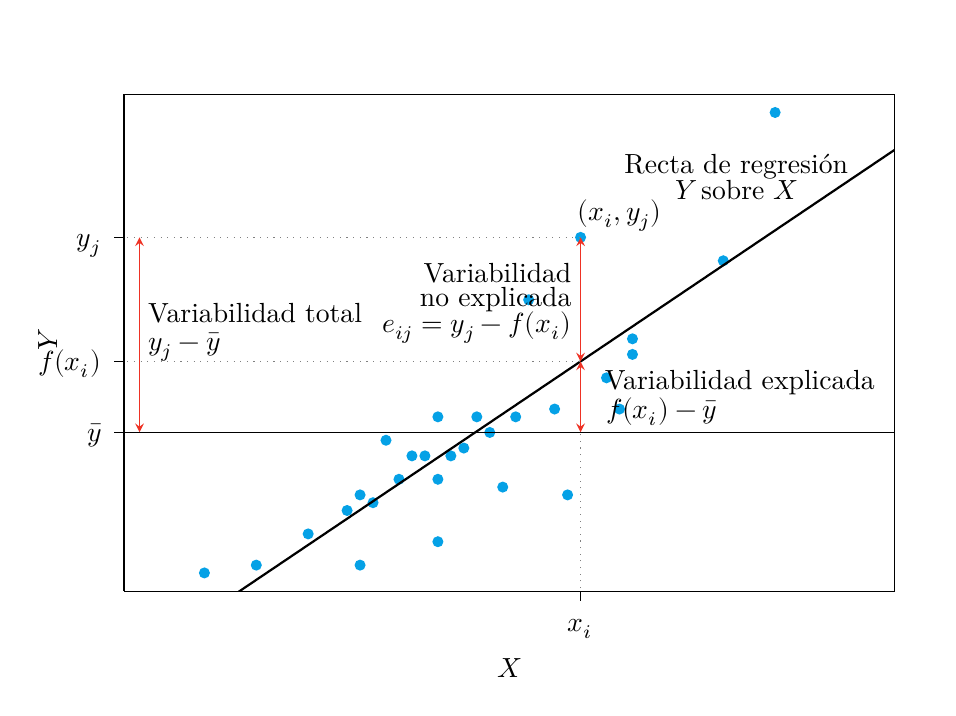
\begin{tikzpicture}[x=1pt,y=1pt]
\begin{scope}
\path[clip] (0.00, 0.00) rectangle (325.21,238.49);
\draw ( 34.80, 34.80) -- 	(313.21, 34.80) -- (313.21,214.49) -- ( 34.80,214.49) -- ( 34.80, 34.80);
\node[anchor=base,] at (174.01,  3.60) {$X$};
\node[rotate= 90.00,anchor=base,] at ( 10.80,124.65) {$Y$};
\end{scope}

% Cloud of points
\begin{scope}
\path[clip] ( 34.80, 34.80) rectangle (313.21,214.49);
\path[fill=color1] (181.04,140.16) circle (2);
\path[fill=color1] (152.92, 83.76) circle (2);
\path[fill=color1] (190.41,100.68) circle (2);
\path[fill=color1] (138.85, 83.76) circle (2);
\path[fill=color1] ( 82.61, 44.28) circle (2);
\path[fill=color1] (157.60, 86.58) circle (2);
\path[fill=color1] (148.23, 75.30) circle (2);
\path[fill=color1] (120.11, 69.66) circle (2);
\path[fill=color1] (251.35,154.26) circle (2);
\path[fill=color1] (209.16,111.96) circle (2);
\path[fill=color1] (101.36, 55.56) circle (2);
\path[fill=color1] (218.54,120.42) circle (2);
\path[fill=color1] (270.09,207.84) circle (2);
\path[fill=color1] (171.66, 72.48) circle (2);
\path[fill=color1] (176.35, 97.86) circle (2);
\path[fill=color1] (115.42, 64.02) circle (2);
\path[fill=color1] ( 63.86, 41.46) circle (2);
\path[fill=color1] (199.79,162.72) circle (2);
\path[fill=color1] (120.11, 44.28) circle (2);
\path[fill=color1] (143.54, 83.76) circle (2);
\path[fill=color1] (162.29, 97.86) circle (2);
\path[fill=color1] (195.10, 69.66) circle (2);
\path[fill=color1] (124.79, 66.84) circle (2);
\path[fill=color1] (134.17, 75.30) circle (2);
\path[fill=color1] (148.23, 97.86) circle (2);
\path[fill=color1] (213.85,100.68) circle (2);
\path[fill=color1] (148.23, 52.74) circle (2);
\path[fill=color1] (166.98, 92.22) circle (2);
\path[fill=color1] (129.48, 89.40) circle (2);
\path[fill=color1] (218.54,126.06) circle (2);
\end{scope}

\begin{scope}
\path[clip] (0.00, 0.00) rectangle (325.21,238.49);
\node[anchor=base,] at (213.85,168.68) {$(x_i,y_j)$};
\draw[visible on=<2->] (34.80, 92.31) -- (31.21, 92.31);
\node[anchor=base east, visible on=<2->] at (30.00, 88.87) {$\bar y$};
\draw (199.79, 34.80) -- (199.79, 31.21);
\node[anchor=base,] at (199.79, 20.40) {$x_i$};
\draw (34.80,162.72) -- (31.21,162.72);
\node[anchor=base east,] at (30.00,159.27) {$y_j$};

\draw[visible on=<6->] (34.80,117.89) -- (31.21,117.89);
\node[anchor=base east, visible on=<5->] at (30.00,114.44) {$f(x_i)$};
\end{scope}

\begin{scope}
\path[clip] ( 34.80, 34.80) rectangle (313.21,214.49);
\draw[dotted, gray] (0.00,162.72) -- (199.79,162.72);
\draw[dotted, gray] (199.79, 0.00) -- (199.79,162.72);
\draw[visible on=<2->] ( 34.80, 92.31) -- (313.21, 92.31);

\draw[<->, color2, visible on=<3->] ( 40.42, 92.31) -- ( 40.42,162.72);
\node[anchor=west, visible on=<3->] at ( 40,135.40) {Variabilidad total};
\node[anchor=west, visible on=<3->] at ( 40,122.94) {$y_j-\bar y$};
% Regression line 
\draw[line width= 0.8pt, visible on=<4->] ( 34.80,  6.74) -- (313.21,194.30);
\node[anchor=base, visible on=<4->] at (256.03,185.62) {Recta de regresión};
\node[anchor=base, visible on=<4->] at (256.03,176.37) {$Y$ sobre $X$};
% Prediction
\draw[dotted, gray, visible on=<5->] (0.00,117.89) -- (199.79,117.89);
 
\draw[<->, color2, visible on=<6->] (199.79, 92.31) -- (199.79,117.89);
\node[anchor=base west, visible on=<6->] at (205,107.84) {Variabilidad explicada};
\node[anchor=base west, visible on=<6->] at (205.47, 97.38) {$f(x_i)-\bar y$};

\draw[<->, color2, visible on=<7->] (199.79,117.89) -- (199.79,162.72);
\node[anchor=base east, visible on=<7->] at (200,146.32) {Variabilidad};
\node[anchor=base east, visible on=<7->] at (200,137.86) {no explicada};
\node[anchor=base east, visible on=<7->] at (200,128.40) {$e_{ij}=y_j-f(x_i)$};
\end{scope}
\end{tikzpicture}
}}
\mode<presentation>{\resizebox{0.9\textwidth}{!}{% Created by tikzDevice version 0.10.1 on 2016-02-27 13:10:16
% !TEX encoding = UTF-8 Unicode
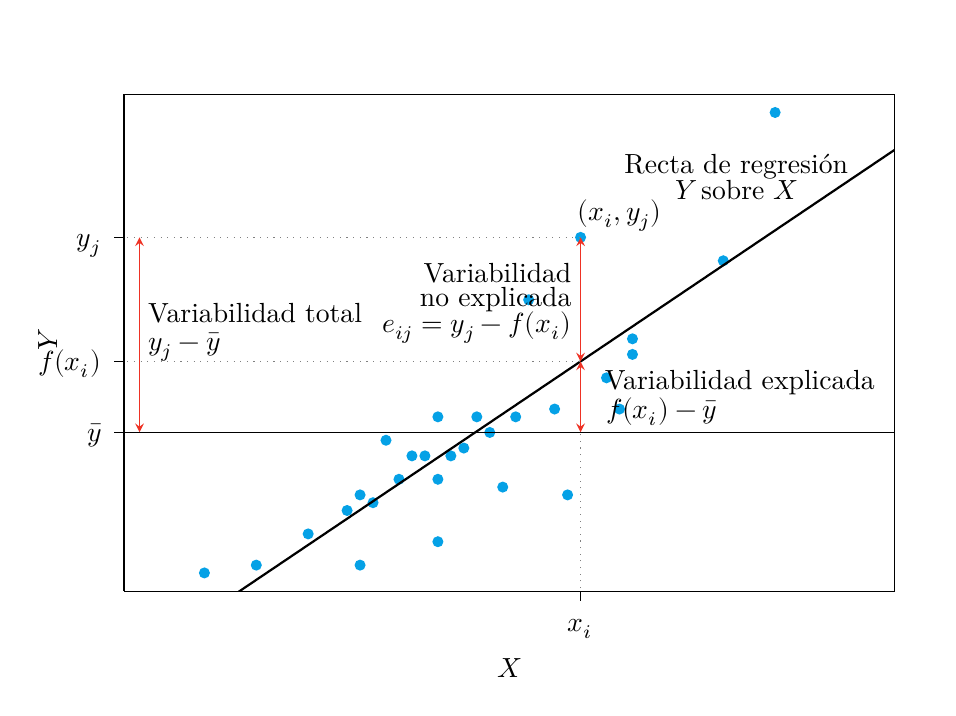
\begin{tikzpicture}[x=1pt,y=1pt]
\begin{scope}
\path[clip] (0.00, 0.00) rectangle (325.21,238.49);
\draw ( 34.80, 34.80) -- 	(313.21, 34.80) -- (313.21,214.49) -- ( 34.80,214.49) -- ( 34.80, 34.80);
\node[anchor=base,] at (174.01,  3.60) {$X$};
\node[rotate= 90.00,anchor=base,] at ( 10.80,124.65) {$Y$};
\end{scope}

% Cloud of points
\begin{scope}
\path[clip] ( 34.80, 34.80) rectangle (313.21,214.49);
\path[fill=color1] (181.04,140.16) circle (2);
\path[fill=color1] (152.92, 83.76) circle (2);
\path[fill=color1] (190.41,100.68) circle (2);
\path[fill=color1] (138.85, 83.76) circle (2);
\path[fill=color1] ( 82.61, 44.28) circle (2);
\path[fill=color1] (157.60, 86.58) circle (2);
\path[fill=color1] (148.23, 75.30) circle (2);
\path[fill=color1] (120.11, 69.66) circle (2);
\path[fill=color1] (251.35,154.26) circle (2);
\path[fill=color1] (209.16,111.96) circle (2);
\path[fill=color1] (101.36, 55.56) circle (2);
\path[fill=color1] (218.54,120.42) circle (2);
\path[fill=color1] (270.09,207.84) circle (2);
\path[fill=color1] (171.66, 72.48) circle (2);
\path[fill=color1] (176.35, 97.86) circle (2);
\path[fill=color1] (115.42, 64.02) circle (2);
\path[fill=color1] ( 63.86, 41.46) circle (2);
\path[fill=color1] (199.79,162.72) circle (2);
\path[fill=color1] (120.11, 44.28) circle (2);
\path[fill=color1] (143.54, 83.76) circle (2);
\path[fill=color1] (162.29, 97.86) circle (2);
\path[fill=color1] (195.10, 69.66) circle (2);
\path[fill=color1] (124.79, 66.84) circle (2);
\path[fill=color1] (134.17, 75.30) circle (2);
\path[fill=color1] (148.23, 97.86) circle (2);
\path[fill=color1] (213.85,100.68) circle (2);
\path[fill=color1] (148.23, 52.74) circle (2);
\path[fill=color1] (166.98, 92.22) circle (2);
\path[fill=color1] (129.48, 89.40) circle (2);
\path[fill=color1] (218.54,126.06) circle (2);
\end{scope}

\begin{scope}
\path[clip] (0.00, 0.00) rectangle (325.21,238.49);
\node[anchor=base,] at (213.85,168.68) {$(x_i,y_j)$};
\draw[visible on=<2->] (34.80, 92.31) -- (31.21, 92.31);
\node[anchor=base east, visible on=<2->] at (30.00, 88.87) {$\bar y$};
\draw (199.79, 34.80) -- (199.79, 31.21);
\node[anchor=base,] at (199.79, 20.40) {$x_i$};
\draw (34.80,162.72) -- (31.21,162.72);
\node[anchor=base east,] at (30.00,159.27) {$y_j$};

\draw[visible on=<6->] (34.80,117.89) -- (31.21,117.89);
\node[anchor=base east, visible on=<5->] at (30.00,114.44) {$f(x_i)$};
\end{scope}

\begin{scope}
\path[clip] ( 34.80, 34.80) rectangle (313.21,214.49);
\draw[dotted, gray] (0.00,162.72) -- (199.79,162.72);
\draw[dotted, gray] (199.79, 0.00) -- (199.79,162.72);
\draw[visible on=<2->] ( 34.80, 92.31) -- (313.21, 92.31);

\draw[<->, color2, visible on=<3->] ( 40.42, 92.31) -- ( 40.42,162.72);
\node[anchor=west, visible on=<3->] at ( 40,135.40) {Variabilidad total};
\node[anchor=west, visible on=<3->] at ( 40,122.94) {$y_j-\bar y$};
% Regression line 
\draw[line width= 0.8pt, visible on=<4->] ( 34.80,  6.74) -- (313.21,194.30);
\node[anchor=base, visible on=<4->] at (256.03,185.62) {Recta de regresión};
\node[anchor=base, visible on=<4->] at (256.03,176.37) {$Y$ sobre $X$};
% Prediction
\draw[dotted, gray, visible on=<5->] (0.00,117.89) -- (199.79,117.89);
 
\draw[<->, color2, visible on=<6->] (199.79, 92.31) -- (199.79,117.89);
\node[anchor=base west, visible on=<6->] at (205,107.84) {Variabilidad explicada};
\node[anchor=base west, visible on=<6->] at (205.47, 97.38) {$f(x_i)-\bar y$};

\draw[<->, color2, visible on=<7->] (199.79,117.89) -- (199.79,162.72);
\node[anchor=base east, visible on=<7->] at (200,146.32) {Variabilidad};
\node[anchor=base east, visible on=<7->] at (200,137.86) {no explicada};
\node[anchor=base east, visible on=<7->] at (200,128.40) {$e_{ij}=y_j-f(x_i)$};
\end{scope}
\end{tikzpicture}
}}
\end{center}

\note{Para interpretar mejor la varianza residual, si dibujamos sobre el diagrama de dispersión, podemos comprobar que la variabilidad de
la variable dependiente depende de las desviaciones de sus valores a su media que en el gráfico aparece representada por esta línea
horizontal. La suma de estas desviaciones la cuadrado, divididas por el tamaño de la muestra nos daba precisamente la varianza de $Y$.

Si ahora dibujamos sobre el diagrama de dispersión el modelo de regresión de $Y$ sobre $X$, en este caso la recta de regresión, podemos
comprobar que la recta divide en dos la desviación de cada valor de $Y$ a su media. Una parte es precisamente el residuo en $Y$, ya que es
la distancia vertical del punto a la recta, y se dice que es la variablidad no explicada por el modelo de regresión, mientras que la otra
parte, la distancia vertical desde la recta a la media de $Y$ se dice que es la variabilidad explicada por el modelo de regresión.

Cuanto mayor sea la variabilidad explicada, menor será la no explicada, es decir menores serán los residuos y mejor explicará el modelo de
regresión la dependencia entre las variables. Cuando el ajuste sea perfecto, la variabilidad no explicada será nula y diremos que el modelo
de regresión de $Y$ sobre $X$ explica toda la variabilidad de $Y$, mientras que cuando no haya relación entre las variables del tipo que
plantee el modelo de regresión, entonces la variablidad explicada será nula y los residuos coincidirán con las desviaciones a la media de
$Y$, de manera que la varianza residual coincidirá con la varianza de $Y$.
}
\end{frame}


\subsection{Coeficientes de determinación y correlación}
%---------------------------------------------------------------------slide----
\begin{frame}
\frametitle{Coeficiente de determinación}
A partir de la varianza residual se puede definir otro estadístico más sencillo de interpretar.
\begin{definicion}[Coeficiente de determinación muestral]
Dado un modelo de regresión simple $y=f(x)$ de una variable bidimensional $(X,Y)$, su \emph{coeficiente de determinación muestral} es
\[
r^2 = 1- \frac{s_{ry}^2}{s_y^2} 
\]
\end{definicion}
Como la varianza residual puede tomar valores entre 0 y $s_y^2$, se tiene que
\[
\alert{0\leq r^2\leq 1}
\]
Cuanto mayor sea $r^2$, mejor explicará el modelo de regresión la relación entre las variables, en particular:
\begin{itemize}
\item Si $r^2 =0$ entonces no existe relación del tipo planteado por el modelo.
\item Si $r^2=1$ entonces la relación que plantea el modelo es perfecta.
\end{itemize}

\note{Como hemos visto, la varianza residual tiene el problema de que es difícil de interpretar porque tiene como unidades las de la
variable dependiente al cuadrado. Teniendo en cuenta, como hemos visto antes, que la varianza residual puede valer entre 0, cuando el
ajueste del modelo de regresión es perfecto, hasta como máximo la varianza de $Y$ cuando entre las variables no hay relación del tipo que
plantea el modelo de regresión, es posible calcular una nueva medida que no tenga unidades y sea más fácil de interpretar. Dicho
estadísticos se llama coeficiente de regresión, se representa por $r^2$ y se define como 1 menos el cociente de la varianza residual entre
la varianza de $Y$.

Como la varianza residual tiene las mismas unidades que la varianza de $Y$, al hacer el cociente las unidades se cancelarán por lo que el
coeficiente de determinación es adimensinal. 

Cuando el ajuste del modelo sea perfecto, la varianza residual valdrá 0 y el cociente también, de manera que el coeficiente de determinación
valdrá 1, mientras que en el otro extremo, cuano no haya relación entre las variables del tipo del modelo de regresión, la varianza residual
coincidirá con la varianza de $Y$ y el cociente valdrá 1, con lo que el coeficiente de determinación valdrá 0.

Así pues, el coeficiente de determinación siempre oscila entre 0 y 1 y será mayor cuanto mejor explique el modelo de regresión la relación
entre las variables. 

Si se multiplica por 100, el coeficiente de determinación nos dará el porcentaje de la variabilidad de la variable dependiente explicado
por el modelo de regresión.}
\end{frame}


%---------------------------------------------------------------------slide----
\begin{frame}
\frametitle{Coeficiente de determinación lineal}
En el caso de las rectas de regresión, la varianza residual vale
\begin{align*}
s_{ry}^2 & = \sum e_{ij}^2f_{ij} = \sum (y_j - f(x_i))^2f_{ij} = \sum \left(y_j - \bar y -\frac{s_{xy}}{s_x^2}(x_i-\bar x) \right)^2f_{ij}=\\
& = \sum \left((y_j - \bar y)^2 +\frac{s_{xy}^2}{s_x^4}(x_i-\bar x)^2 - 2\frac{s_{xy}}{s_x^2}(x_i-\bar x)(y_j -\bar y)\right)f_{ij} =\\ 
& = \sum (y_j - \bar y)^2f_{ij} +\frac{s_{xy}^2}{s_x^4}\sum (x_i-\bar x)^2f_{ij}- 2\frac{s_{xy}}{s_x^2}\sum (x_i-\bar x)(y_j -\bar y)f_{ij}=\\
& = s_y^2 + \frac{s_{xy}^2}{s_x^4}s_x^2 - 2 \frac{s_{xy}}{s_x^2}s_{xy} = s_y^2 - \frac{s_{xy}^2}{s_x^2}.
\end{align*}
y, por tanto, el coeficiente de determinación lineal vale
\begin{align*}
r^2 &= 1- \frac{s_{ry}^2}{s_y^2} = 1- \frac{s_y^2 - \frac{s_{xy}^2}{s_x^2}}{s_y^2} = 1 - 1 + \frac{s_{xy}^2}{s_x^2s_y^2} = \frac{s_{xy}^2}{s_x^2s_y^2}.
\end{align*}

\note{En el caso del ajuste de un modelo lineal, teniendo en cuenta la ecuación de la recta de regresión de $Y$ sobre $X$, los residuos
serán $y_j$ menos el valor de la recta de regresión para $x_i$, es decir $y_j - \bar y -\frac{s_{xy}}{s_x^2}(x_i-\bar x)$. Si en la fórmula
de la varianza residual desarrollamos el cuadrado de estos residuos, y simplificamos, llegamos a que la varianza residual para el modelo
lineal se puede calcular como la varianza de $Y$ menos la covarianza al cuadrado entre la varianza de $X$. Y si sustituimos en la fórmula
del coeficiente de determinación, obtenemos que el coeficiente de determinación lineal puede calcularse como la covarianza al cuadrado entre
el producto de las varianzas de $X$ e $Y$.
}
\end{frame}


%---------------------------------------------------------------------slide----
\begin{frame}
\frametitle{Cálculo del coeficiente de determinación lineal}
\framesubtitle{Ejemplo de estaturas y pesos}
En el ejemplo de las estaturas y pesos se tenía
\[
\begin{array}{lll}
\bar x = 174.67 \mbox{ cm} & \quad & s^2_x = 102.06 \mbox{ cm}^2\\
\bar y = 69.67 \mbox{ Kg} & & s^2_y = 164.42 \mbox{ Kg}^2\\
s_{xy} = 104.07 \mbox{ cm$\cdot$Kg}
\end{array}
\]
De modo que el coeficiente de determinación lineal vale
\[
r^2 = \frac{s_{xy}^2}{s_x^2s_y^2} = \frac{(104.07 \mbox{ cm$\cdot$Kg})^2}{102.06 \mbox{ cm}^2 \cdot 164.42 \mbox{ Kg}^2} = 0.65.
\]
Esto indica que la recta de regresión del peso sobre la estatura explica el 65\% de la variabilidad del peso, y de igual modo, la recta de regresión de la estatura sobre el peso explica el  65\% de la variabilidad de la estatura.
\note{En el ejemplo de las estaturas y los pesos, como la covarianza valía $104.7$ cm por kg, la varianza de la estatura era $102.06$ kg$^2$
y la varianza del peso era $164.42$ kg$^2$, el coeficiente de determinación lineal valdrá 
\[
r^2 = \frac{(104.07 \mbox{ cm$\cdot$Kg})^2}{102.06 \mbox{ cm}^2 \cdot 164.42 \mbox{ Kg}^2} = 0.65,
\]
lo que indica que la recta de regresión del peso sobre la estatura explica el 65\% de la variabilidad del peso, y de igual modo, la recta de
regresión de la estatura sobre el peso explica el  65\% de la variabilidad de la estatura.
}
\end{frame}


%---------------------------------------------------------------------slide----
\begin{frame}
\frametitle{Coeficiente de correlación lineal}
\begin{definicion}[Coeficiente de correlación lineal]
Dada una variable bidimensional $(X,Y)$, el \emph{coeficiente de correlación lineal muestral} es
la raíz cuadrada de su coeficiente de determinación lineal, con signo el de la covarianza
\[
r = \sqrt{r^2} = \dfrac{s_{xy}}{s_xs_y}. 
\]
\end{definicion}
Como $r^2$ toma valores entre 0 y 1, $r$ tomará valores entre -1 y 1:
\[
\alert{-1\leq r\leq 1}
\]
El coeficiente de correlación lineal no sólo mide mide el grado de dependencia lineal sino también su dirección (creciente o decreciente):
\begin{itemize}
\item Si $r =0$ entonces no existe relación lineal.
\item Si $r=1$ entonces existe una relación lineal creciente perfecta.
\item Si $r=-1$ entonces existe una relación lineal decreciente perfecta.
\end{itemize}

\note{Otra media habitual del grado de relación lineal entre dos variables es el coeficiente de correlación lineal, es la raíz cuadrada del
coeficiente de determinación lineal y por tanto se calcula dividiendo la covarianza entre el producto de las desviaciones típicas de $X$ e
$Y$.

Como el coeficiente de determinación podía tomar valores entre 0 y 1, el coeficiente de correlación lineal tomará valores entre -1 y 1, de
manera que un cuando no haya relación lineal entre las variables valdrá 0, cuando haya una relación lineal creciente perfecta valdrá 1
y cuado haya una relación lineal decreciente perfecta valdrá -1. 
}
\end{frame}


%---------------------------------------------------------------------slide----
\begin{frame}
\frametitle{Coeficiente de correlación lineal}
\framesubtitle{Ejemplo}
En el ejemplo de las estaturas y los pesos se tenía 
\[
\begin{array}{lll}
\bar x = 174.67 \mbox{ cm} & \quad & s^2_x = 102.06 \mbox{ cm}^2\\
\bar y = 69.67 \mbox{ Kg} & & s^2_y = 164.42 \mbox{ Kg}^2\\
s_{xy} = 104.07 \mbox{ cm$\cdot$Kg}
\end{array}
\]
De modo que el coeficiente de correlación lineal vale
\[
r = \frac{s_{xy}}{s_xs_y} = \frac{104.07 \mbox{ cm$\cdot$Kg}}{10.1 \mbox{ cm} \cdot 12.82 \mbox{ Kg}} = +0.8.
\]
Esto indica que la relación lineal entre el peso y la estatura es fuerte, y además creciente.

\note{
Por ejemplo, en el caso de las estaturas y los pesos, el coeficiente de correlación lineal vale 
\[
r = \frac{104.07 \mbox{ cm$\cdot$Kg}}{10.1 \mbox{ cm} \cdot 12.82 \mbox{ Kg}} = +0.8.
\]
lo que indica que la relación lineal entre el peso y la estatura es fuerte, y además creciente.
}
\end{frame}



%---------------------------------------------------------------------slide----
\begin{frame}
\frametitle{Distintos grados de correlación}
\centering
\tikzsetnextfilename{regresion/grados_correlacion}
\resizebox{\textwidth}{!}{% Created by tikzDevice version 0.10.1 on 2016-02-27 13:14:33
% !TEX encoding = UTF-8 Unicode
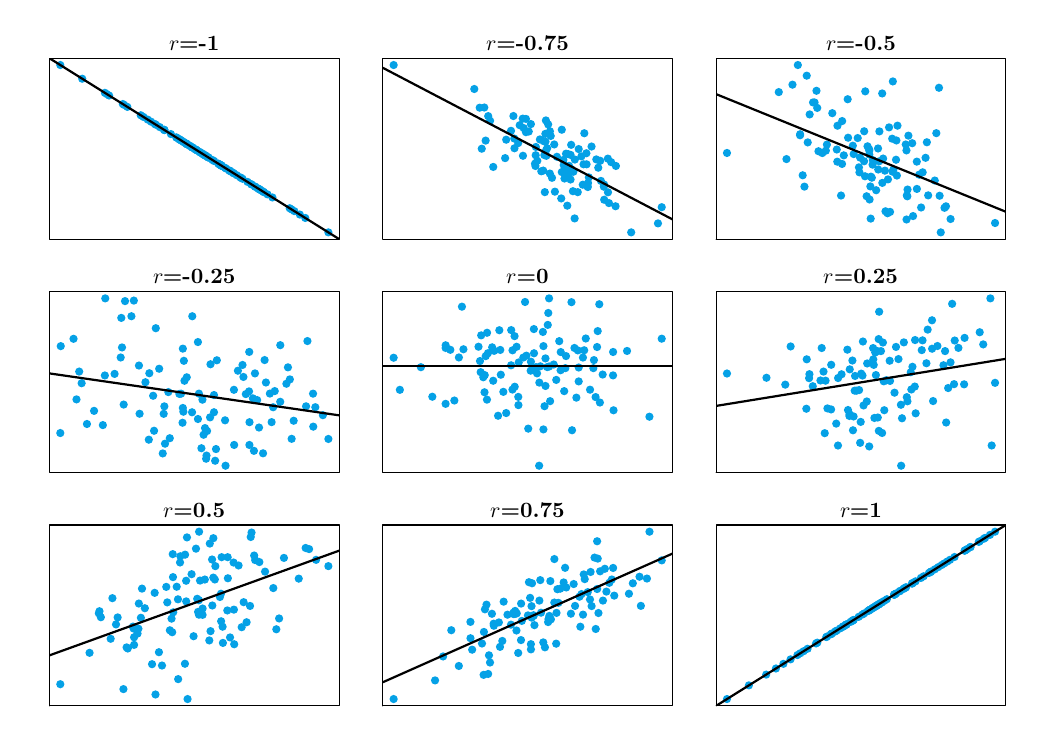
\begin{tikzpicture}[x=1pt,y=1pt]
\definecolor{fillColor}{RGB}{255,255,255}
\path[use as bounding box,fill=fillColor,fill opacity=0.00] (0,0) rectangle (361.35,252.94);
\begin{scope}
\path[clip] (  7.92,176.55) rectangle (112.53,241.86);
\definecolor{fillColor}{RGB}{5,161,230}

\path[fill=fillColor] ( 34.83,225.06) circle (  1.49);

\path[fill=fillColor] ( 57.37,210.99) circle (  1.49);

\path[fill=fillColor] ( 47.72,217.01) circle (  1.49);

\path[fill=fillColor] ( 60.53,209.02) circle (  1.49);

\path[fill=fillColor] ( 68.84,203.83) circle (  1.49);

\path[fill=fillColor] ( 69.51,203.41) circle (  1.49);

\path[fill=fillColor] ( 59.64,209.57) circle (  1.49);

\path[fill=fillColor] ( 56.31,211.65) circle (  1.49);

\path[fill=fillColor] ( 46.35,217.87) circle (  1.49);

\path[fill=fillColor] ( 49.43,215.94) circle (  1.49);

\path[fill=fillColor] ( 55.63,212.07) circle (  1.49);

\path[fill=fillColor] ( 63.20,207.35) circle (  1.49);

\path[fill=fillColor] ( 70.11,203.03) circle (  1.49);

\path[fill=fillColor] ( 63.40,207.22) circle (  1.49);

\path[fill=fillColor] ( 57.58,210.86) circle (  1.49);

\path[fill=fillColor] ( 28.57,228.97) circle (  1.49);

\path[fill=fillColor] ( 95.36,187.27) circle (  1.49);

\path[fill=fillColor] ( 71.32,202.28) circle (  1.49);

\path[fill=fillColor] ( 54.58,212.73) circle (  1.49);

\path[fill=fillColor] ( 58.68,210.17) circle (  1.49);

\path[fill=fillColor] ( 64.07,206.80) circle (  1.49);

\path[fill=fillColor] ( 96.35,186.65) circle (  1.49);

\path[fill=fillColor] ( 45.95,218.12) circle (  1.49);

\path[fill=fillColor] ( 29.44,228.42) circle (  1.49);

\path[fill=fillColor] ( 69.90,203.16) circle (  1.49);

\path[fill=fillColor] ( 63.45,207.19) circle (  1.49);

\path[fill=fillColor] ( 57.14,211.13) circle (  1.49);

\path[fill=fillColor] ( 65.11,206.15) circle (  1.49);

\path[fill=fillColor] ( 53.67,213.30) circle (  1.49);

\path[fill=fillColor] ( 57.52,210.89) circle (  1.49);

\path[fill=fillColor] ( 65.40,205.97) circle (  1.49);

\path[fill=fillColor] ( 61.18,208.61) circle (  1.49);

\path[fill=fillColor] ( 58.49,210.29) circle (  1.49);

\path[fill=fillColor] ( 44.58,218.97) circle (  1.49);

\path[fill=fillColor] ( 27.90,229.39) circle (  1.49);

\path[fill=fillColor] ( 85.37,193.50) circle (  1.49);

\path[fill=fillColor] ( 83.86,194.45) circle (  1.49);

\path[fill=fillColor] ( 59.50,209.65) circle (  1.49);

\path[fill=fillColor] ( 55.34,212.25) circle (  1.49);

\path[fill=fillColor] ( 88.44,191.59) circle (  1.49);

\path[fill=fillColor] ( 75.54,199.64) circle (  1.49);

\path[fill=fillColor] ( 72.90,201.29) circle (  1.49);

\path[fill=fillColor] ( 62.28,207.92) circle (  1.49);

\path[fill=fillColor] ( 62.15,208.00) circle (  1.49);

\path[fill=fillColor] ( 40.86,221.29) circle (  1.49);

\path[fill=fillColor] ( 77.09,198.68) circle (  1.49);

\path[fill=fillColor] ( 57.64,210.81) circle (  1.49);

\path[fill=fillColor] ( 73.60,200.86) circle (  1.49);

\path[fill=fillColor] ( 64.40,206.60) circle (  1.49);

\path[fill=fillColor] ( 19.71,234.49) circle (  1.49);

\path[fill=fillColor] ( 62.68,207.67) circle (  1.49);

\path[fill=fillColor] ( 80.77,196.38) circle (  1.49);

\path[fill=fillColor] ( 60.71,208.90) circle (  1.49);

\path[fill=fillColor] ( 74.29,200.42) circle (  1.49);

\path[fill=fillColor] ( 76.85,198.82) circle (  1.49);

\path[fill=fillColor] ( 41.84,220.68) circle (  1.49);

\path[fill=fillColor] ( 56.42,211.58) circle (  1.49);

\path[fill=fillColor] ( 94.68,187.69) circle (  1.49);

\path[fill=fillColor] ( 74.46,200.32) circle (  1.49);

\path[fill=fillColor] ( 49.25,216.06) circle (  1.49);

\path[fill=fillColor] ( 54.81,212.59) circle (  1.49);

\path[fill=fillColor] ( 63.92,206.89) circle (  1.49);

\path[fill=fillColor] ( 83.44,194.71) circle (  1.49);

\path[fill=fillColor] ( 64.34,206.63) circle (  1.49);

\path[fill=fillColor] ( 53.90,213.15) circle (  1.49);

\path[fill=fillColor] ( 69.22,203.59) circle (  1.49);

\path[fill=fillColor] ( 80.89,196.31) circle (  1.49);

\path[fill=fillColor] ( 57.29,211.03) circle (  1.49);

\path[fill=fillColor] ( 83.19,194.87) circle (  1.49);

\path[fill=fillColor] ( 77.65,198.33) circle (  1.49);

\path[fill=fillColor] ( 73.07,201.18) circle (  1.49);

\path[fill=fillColor] ( 86.67,192.70) circle (  1.49);

\path[fill=fillColor] ( 66.77,205.11) circle (  1.49);

\path[fill=fillColor] ( 51.75,214.49) circle (  1.49);

\path[fill=fillColor] ( 61.09,208.66) circle (  1.49);

\path[fill=fillColor] ( 36.02,224.31) circle (  1.49);

\path[fill=fillColor] ( 98.35,185.40) circle (  1.49);

\path[fill=fillColor] ( 59.45,209.69) circle (  1.49);

\path[fill=fillColor] ( 11.79,239.44) circle (  1.49);

\path[fill=fillColor] ( 34.38,225.34) circle (  1.49);

\path[fill=fillColor] ( 79.44,197.21) circle (  1.49);

\path[fill=fillColor] ( 65.23,206.08) circle (  1.49);

\path[fill=fillColor] ( 69.73,203.27) circle (  1.49);

\path[fill=fillColor] ( 43.38,219.72) circle (  1.49);

\path[fill=fillColor] (108.66,178.97) circle (  1.49);

\path[fill=fillColor] ( 49.38,215.98) circle (  1.49);

\path[fill=fillColor] ( 70.16,203.00) circle (  1.49);

\path[fill=fillColor] ( 85.12,193.66) circle (  1.49);

\path[fill=fillColor] (100.31,184.18) circle (  1.49);

\path[fill=fillColor] ( 59.36,209.74) circle (  1.49);

\path[fill=fillColor] ( 84.57,194.00) circle (  1.49);

\path[fill=fillColor] ( 71.71,202.03) circle (  1.49);

\path[fill=fillColor] ( 82.23,195.47) circle (  1.49);

\path[fill=fillColor] ( 82.12,195.53) circle (  1.49);

\path[fill=fillColor] ( 70.13,203.02) circle (  1.49);

\path[fill=fillColor] ( 73.04,201.20) circle (  1.49);

\path[fill=fillColor] ( 55.07,212.42) circle (  1.49);

\path[fill=fillColor] ( 83.92,194.41) circle (  1.49);

\path[fill=fillColor] ( 69.38,203.49) circle (  1.49);

\path[fill=fillColor] ( 67.35,204.76) circle (  1.49);
\end{scope}
\begin{scope}
\path[clip] (  0.00,168.63) rectangle (120.45,252.94);
\definecolor{drawColor}{RGB}{0,0,0}

\node[text=drawColor,anchor=base,inner sep=0pt, outer sep=0pt, scale=  0.79] at ( 60.22,244.63) {\bfseries $r$=-1};

\node[text=drawColor,anchor=base,inner sep=0pt, outer sep=0pt, scale=  0.66] at ( 60.22,146.45) {$X$};
\end{scope}
\begin{scope}
\path[clip] (  7.92,176.55) rectangle (112.53,241.86);
\definecolor{drawColor}{RGB}{0,0,0}

\path[draw=drawColor,line width= 0.8pt,line join=round,line cap=round] (  7.92,241.86) -- (112.53,176.55);
\end{scope}
\begin{scope}
\path[clip] (  0.00,  0.00) rectangle (361.35,252.94);
\definecolor{drawColor}{RGB}{0,0,0}

\path[draw=drawColor,line width= 0.4pt,line join=round,line cap=round] (  7.92,176.55) --
	(112.53,176.55) --
	(112.53,241.86) --
	(  7.92,241.86) --
	(  7.92,176.55);
\end{scope}
\begin{scope}
\path[clip] (128.37,176.55) rectangle (232.98,241.86);
\definecolor{fillColor}{RGB}{5,161,230}

\path[fill=fillColor] (196.17,198.07) circle (  1.49);

\path[fill=fillColor] (208.32,190.76) circle (  1.49);

\path[fill=fillColor] (183.57,206.85) circle (  1.49);

\path[fill=fillColor] (174.65,215.66) circle (  1.49);

\path[fill=fillColor] (218.08,178.97) circle (  1.49);

\path[fill=fillColor] (167.10,219.28) circle (  1.49);

\path[fill=fillColor] (199.11,209.08) circle (  1.49);

\path[fill=fillColor] (201.96,203.56) circle (  1.49);

\path[fill=fillColor] (186.70,206.91) circle (  1.49);

\path[fill=fillColor] (201.89,207.56) circle (  1.49);

\path[fill=fillColor] (181.84,218.10) circle (  1.49);

\path[fill=fillColor] (205.48,205.33) circle (  1.49);

\path[fill=fillColor] (206.88,204.83) circle (  1.49);

\path[fill=fillColor] (172.91,212.46) circle (  1.49);

\path[fill=fillColor] (178.88,220.07) circle (  1.49);

\path[fill=fillColor] (198.77,193.50) circle (  1.49);

\path[fill=fillColor] (192.80,191.23) circle (  1.49);

\path[fill=fillColor] (187.06,214.58) circle (  1.49);

\path[fill=fillColor] (172.53,205.80) circle (  1.49);

\path[fill=fillColor] (187.33,208.67) circle (  1.49);

\path[fill=fillColor] (227.76,182.22) circle (  1.49);

\path[fill=fillColor] (161.38,230.78) circle (  1.49);

\path[fill=fillColor] (188.69,200.21) circle (  1.49);

\path[fill=fillColor] (208.18,195.48) circle (  1.49);

\path[fill=fillColor] (183.64,209.83) circle (  1.49);

\path[fill=fillColor] (165.48,212.13) circle (  1.49);

\path[fill=fillColor] (189.46,198.68) circle (  1.49);

\path[fill=fillColor] (132.24,239.44) circle (  1.49);

\path[fill=fillColor] (178.97,206.65) circle (  1.49);

\path[fill=fillColor] (175.84,212.87) circle (  1.49);

\path[fill=fillColor] (191.24,206.28) circle (  1.49);

\path[fill=fillColor] (196.18,206.97) circle (  1.49);

\path[fill=fillColor] (179.24,216.66) circle (  1.49);

\path[fill=fillColor] (183.32,203.80) circle (  1.49);

\path[fill=fillColor] (187.11,211.75) circle (  1.49);

\path[fill=fillColor] (181.07,215.41) circle (  1.49);

\path[fill=fillColor] (190.51,193.68) circle (  1.49);

\path[fill=fillColor] (186.87,193.51) circle (  1.49);

\path[fill=fillColor] (210.04,189.55) circle (  1.49);

\path[fill=fillColor] (208.29,196.24) circle (  1.49);

\path[fill=fillColor] (212.56,202.97) circle (  1.49);

\path[fill=fillColor] (195.16,199.85) circle (  1.49);

\path[fill=fillColor] (202.28,195.68) circle (  1.49);

\path[fill=fillColor] (193.58,205.14) circle (  1.49);

\path[fill=fillColor] (185.59,201.05) circle (  1.49);

\path[fill=fillColor] (186.43,211.94) circle (  1.49);

\path[fill=fillColor] (194.99,188.62) circle (  1.49);

\path[fill=fillColor] (175.90,209.36) circle (  1.49);

\path[fill=fillColor] (180.04,215.18) circle (  1.49);

\path[fill=fillColor] (210.84,204.34) circle (  1.49);

\path[fill=fillColor] (187.26,219.42) circle (  1.49);

\path[fill=fillColor] (206.18,202.33) circle (  1.49);

\path[fill=fillColor] (193.70,203.27) circle (  1.49);

\path[fill=fillColor] (202.49,196.82) circle (  1.49);

\path[fill=fillColor] (193.98,198.43) circle (  1.49);

\path[fill=fillColor] (168.23,202.62) circle (  1.49);

\path[fill=fillColor] (188.71,215.51) circle (  1.49);

\path[fill=fillColor] (196.39,210.60) circle (  1.49);

\path[fill=fillColor] (190.27,210.74) circle (  1.49);

\path[fill=fillColor] (200.86,203.57) circle (  1.49);

\path[fill=fillColor] (183.48,202.96) circle (  1.49);

\path[fill=fillColor] (195.27,207.26) circle (  1.49);

\path[fill=fillColor] (163.34,224.02) circle (  1.49);

\path[fill=fillColor] (207.15,197.57) circle (  1.49);

\path[fill=fillColor] (193.01,200.76) circle (  1.49);

\path[fill=fillColor] (196.41,201.81) circle (  1.49);

\path[fill=fillColor] (185.09,212.55) circle (  1.49);

\path[fill=fillColor] (202.77,198.85) circle (  1.49);

\path[fill=fillColor] (175.52,221.01) circle (  1.49);

\path[fill=fillColor] (195.62,203.01) circle (  1.49);

\path[fill=fillColor] (177.80,217.70) circle (  1.49);

\path[fill=fillColor] (202.39,195.35) circle (  1.49);

\path[fill=fillColor] (187.42,206.64) circle (  1.49);

\path[fill=fillColor] (197.02,193.85) circle (  1.49);

\path[fill=fillColor] (180.05,219.97) circle (  1.49);

\path[fill=fillColor] (166.41,220.98) circle (  1.49);

\path[fill=fillColor] (200.08,206.43) circle (  1.49);

\path[fill=fillColor] (197.71,205.28) circle (  1.49);

\path[fill=fillColor] (212.43,188.41) circle (  1.49);

\path[fill=fillColor] (165.00,224.09) circle (  1.49);

\path[fill=fillColor] (187.71,209.37) circle (  1.49);

\path[fill=fillColor] (193.00,216.06) circle (  1.49);

\path[fill=fillColor] (209.65,205.62) circle (  1.49);

\path[fill=fillColor] (186.29,201.29) circle (  1.49);

\path[fill=fillColor] (197.64,184.01) circle (  1.49);

\path[fill=fillColor] (200.58,196.19) circle (  1.49);

\path[fill=fillColor] (189.00,213.81) circle (  1.49);

\path[fill=fillColor] (193.84,201.35) circle (  1.49);

\path[fill=fillColor] (195.45,200.56) circle (  1.49);

\path[fill=fillColor] (209.69,193.45) circle (  1.49);

\path[fill=fillColor] (188.08,217.99) circle (  1.49);

\path[fill=fillColor] (194.53,207.39) circle (  1.49);

\path[fill=fillColor] (229.11,188.07) circle (  1.49);

\path[fill=fillColor] (164.08,209.20) circle (  1.49);

\path[fill=fillColor] (184.16,204.83) circle (  1.49);

\path[fill=fillColor] (201.14,214.79) circle (  1.49);

\path[fill=fillColor] (203.76,209.99) circle (  1.49);

\path[fill=fillColor] (197.20,200.87) circle (  1.49);

\path[fill=fillColor] (177.25,211.24) circle (  1.49);

\path[fill=fillColor] (196.25,200.79) circle (  1.49);
\end{scope}
\begin{scope}
\path[clip] (120.45,168.63) rectangle (240.90,252.94);
\definecolor{drawColor}{RGB}{0,0,0}

\node[text=drawColor,anchor=base,inner sep=0pt, outer sep=0pt, scale=  0.79] at (180.68,244.63) {\bfseries $r$=-0.75};

\node[text=drawColor,anchor=base,inner sep=0pt, outer sep=0pt, scale=  0.66] at (180.68,146.45) {$X$};

\node[text=drawColor,rotate= 90.00,anchor=base,inner sep=0pt, outer sep=0pt, scale=  0.66] at (103.03,209.20) {$Y$};
\end{scope}
\begin{scope}
\path[clip] (128.37,176.55) rectangle (232.98,241.86);
\definecolor{drawColor}{RGB}{0,0,0}

\path[draw=drawColor,line width= 0.8pt,line join=round,line cap=round] (128.37,238.41) -- (232.98,183.67);
\end{scope}
\begin{scope}
\path[clip] (  0.00,  0.00) rectangle (361.35,252.94);
\definecolor{drawColor}{RGB}{0,0,0}

\path[draw=drawColor,line width= 0.4pt,line join=round,line cap=round] (128.37,176.55) --
	(232.98,176.55) --
	(232.98,241.86) --
	(128.37,241.86) --
	(128.37,176.55);
\end{scope}
\begin{scope}
\path[clip] (248.82,176.55) rectangle (353.43,241.86);
\definecolor{fillColor}{RGB}{5,161,230}

\path[fill=fillColor] (299.93,213.05) circle (  1.49);

\path[fill=fillColor] (324.45,205.91) circle (  1.49);

\path[fill=fillColor] (298.48,207.26) circle (  1.49);

\path[fill=fillColor] (284.35,225.91) circle (  1.49);

\path[fill=fillColor] (324.92,211.53) circle (  1.49);

\path[fill=fillColor] (252.69,207.66) circle (  1.49);

\path[fill=fillColor] (305.39,205.08) circle (  1.49);

\path[fill=fillColor] (303.15,192.02) circle (  1.49);

\path[fill=fillColor] (312.83,201.68) circle (  1.49);

\path[fill=fillColor] (329.94,178.97) circle (  1.49);

\path[fill=fillColor] (309.12,205.64) circle (  1.49);

\path[fill=fillColor] (292.55,204.51) circle (  1.49);

\path[fill=fillColor] (294.27,203.70) circle (  1.49);

\path[fill=fillColor] (288.80,210.69) circle (  1.49);

\path[fill=fillColor] (296.46,213.17) circle (  1.49);

\path[fill=fillColor] (304.07,209.01) circle (  1.49);

\path[fill=fillColor] (313.78,205.21) circle (  1.49);

\path[fill=fillColor] (281.87,211.48) circle (  1.49);

\path[fill=fillColor] (300.79,205.99) circle (  1.49);

\path[fill=fillColor] (311.62,186.36) circle (  1.49);

\path[fill=fillColor] (302.57,199.24) circle (  1.49);

\path[fill=fillColor] (313.91,212.18) circle (  1.49);

\path[fill=fillColor] (309.97,186.59) circle (  1.49);

\path[fill=fillColor] (285.30,223.94) circle (  1.49);

\path[fill=fillColor] (285.03,230.13) circle (  1.49);

\path[fill=fillColor] (302.66,229.93) circle (  1.49);

\path[fill=fillColor] (305.03,198.72) circle (  1.49);

\path[fill=fillColor] (302.27,215.50) circle (  1.49);

\path[fill=fillColor] (333.49,183.80) circle (  1.49);

\path[fill=fillColor] (304.23,190.85) circle (  1.49);

\path[fill=fillColor] (314.30,217.53) circle (  1.49);

\path[fill=fillColor] (298.17,210.28) circle (  1.49);

\path[fill=fillColor] (312.51,200.90) circle (  1.49);

\path[fill=fillColor] (309.76,201.27) circle (  1.49);

\path[fill=fillColor] (294.90,206.80) circle (  1.49);

\path[fill=fillColor] (318.25,213.92) circle (  1.49);

\path[fill=fillColor] (308.78,229.17) circle (  1.49);

\path[fill=fillColor] (310.87,198.12) circle (  1.49);

\path[fill=fillColor] (319.93,184.86) circle (  1.49);

\path[fill=fillColor] (304.50,195.58) circle (  1.49);

\path[fill=fillColor] (331.82,188.39) circle (  1.49);

\path[fill=fillColor] (329.53,192.20) circle (  1.49);

\path[fill=fillColor] (290.75,222.04) circle (  1.49);

\path[fill=fillColor] (307.34,201.69) circle (  1.49);

\path[fill=fillColor] (307.76,215.46) circle (  1.49);

\path[fill=fillColor] (305.31,203.44) circle (  1.49);

\path[fill=fillColor] (317.58,183.62) circle (  1.49);

\path[fill=fillColor] (323.40,200.67) circle (  1.49);

\path[fill=fillColor] (329.30,231.22) circle (  1.49);

\path[fill=fillColor] (300.38,202.46) circle (  1.49);

\path[fill=fillColor] (303.48,210.07) circle (  1.49);

\path[fill=fillColor] (276.36,232.34) circle (  1.49);

\path[fill=fillColor] (285.75,208.29) circle (  1.49);

\path[fill=fillColor] (306.60,194.20) circle (  1.49);

\path[fill=fillColor] (317.55,208.59) circle (  1.49);

\path[fill=fillColor] (319.62,211.19) circle (  1.49);

\path[fill=fillColor] (304.11,208.50) circle (  1.49);

\path[fill=fillColor] (317.29,210.73) circle (  1.49);

\path[fill=fillColor] (317.69,192.36) circle (  1.49);

\path[fill=fillColor] (328.34,214.82) circle (  1.49);

\path[fill=fillColor] (302.22,204.67) circle (  1.49);

\path[fill=fillColor] (279.12,214.43) circle (  1.49);

\path[fill=fillColor] (321.29,204.53) circle (  1.49);

\path[fill=fillColor] (283.79,225.92) circle (  1.49);

\path[fill=fillColor] (304.70,199.10) circle (  1.49);

\path[fill=fillColor] (325.39,192.34) circle (  1.49);

\path[fill=fillColor] (288.42,208.50) circle (  1.49);

\path[fill=fillColor] (281.51,235.59) circle (  1.49);

\path[fill=fillColor] (307.28,209.29) circle (  1.49);

\path[fill=fillColor] (322.84,187.96) circle (  1.49);

\path[fill=fillColor] (274.19,205.45) circle (  1.49);

\path[fill=fillColor] (312.63,233.51) circle (  1.49);

\path[fill=fillColor] (279.10,214.07) circle (  1.49);

\path[fill=fillColor] (310.70,185.88) circle (  1.49);

\path[fill=fillColor] (293.91,192.28) circle (  1.49);

\path[fill=fillColor] (317.86,192.00) circle (  1.49);

\path[fill=fillColor] (317.94,194.44) circle (  1.49);

\path[fill=fillColor] (321.31,194.67) circle (  1.49);

\path[fill=fillColor] (308.83,196.85) circle (  1.49);

\path[fill=fillColor] (296.31,227.08) circle (  1.49);

\path[fill=fillColor] (294.31,219.19) circle (  1.49);

\path[fill=fillColor] (300.56,200.65) circle (  1.49);

\path[fill=fillColor] (287.14,207.63) circle (  1.49);

\path[fill=fillColor] (280.68,195.50) circle (  1.49);

\path[fill=fillColor] (292.62,217.51) circle (  1.49);

\path[fill=fillColor] (278.30,239.44) circle (  1.49);

\path[fill=fillColor] (322.14,199.82) circle (  1.49);

\path[fill=fillColor] (282.57,221.59) circle (  1.49);

\path[fill=fillColor] (304.12,207.11) circle (  1.49);

\path[fill=fillColor] (331.29,187.84) circle (  1.49);

\path[fill=fillColor] (304.62,183.94) circle (  1.49);

\path[fill=fillColor] (314.09,199.50) circle (  1.49);

\path[fill=fillColor] (311.26,216.91) circle (  1.49);

\path[fill=fillColor] (349.56,182.35) circle (  1.49);

\path[fill=fillColor] (292.37,208.91) circle (  1.49);

\path[fill=fillColor] (307.71,204.66) circle (  1.49);

\path[fill=fillColor] (280.05,199.60) circle (  1.49);

\path[fill=fillColor] (271.41,229.66) circle (  1.49);

\path[fill=fillColor] (327.78,197.70) circle (  1.49);

\path[fill=fillColor] (312.39,212.82) circle (  1.49);
\end{scope}
\begin{scope}
\path[clip] (240.90,168.63) rectangle (361.35,252.94);
\definecolor{drawColor}{RGB}{0,0,0}

\node[text=drawColor,anchor=base,inner sep=0pt, outer sep=0pt, scale=  0.79] at (301.12,244.63) {\bfseries $r$=-0.5};

\node[text=drawColor,anchor=base,inner sep=0pt, outer sep=0pt, scale=  0.66] at (301.12,146.45) {$X$};

\node[text=drawColor,rotate= 90.00,anchor=base,inner sep=0pt, outer sep=0pt, scale=  0.66] at (223.48,209.20) {$Y$};
\end{scope}
\begin{scope}
\path[clip] (248.82,176.55) rectangle (353.43,241.86);
\definecolor{drawColor}{RGB}{0,0,0}

\path[draw=drawColor,line width= 0.8pt,line join=round,line cap=round] (248.82,228.90) -- (353.43,186.43);
\end{scope}
\begin{scope}
\path[clip] (  0.00,  0.00) rectangle (361.35,252.94);
\definecolor{drawColor}{RGB}{0,0,0}

\path[draw=drawColor,line width= 0.4pt,line join=round,line cap=round] (248.82,176.55) --
	(353.43,176.55) --
	(353.43,241.86) --
	(248.82,241.86) --
	(248.82,176.55);
\end{scope}
\begin{scope}
\path[clip] (  7.92, 92.23) rectangle (112.53,157.54);
\definecolor{fillColor}{RGB}{5,161,230}

\path[fill=fillColor] ( 88.70,115.78) circle (  1.49);

\path[fill=fillColor] ( 28.04,155.12) circle (  1.49);

\path[fill=fillColor] ( 71.33,111.06) circle (  1.49);

\path[fill=fillColor] ( 56.07,136.96) circle (  1.49);

\path[fill=fillColor] ( 64.83,107.20) circle (  1.49);

\path[fill=fillColor] ( 16.57,140.51) circle (  1.49);

\path[fill=fillColor] ( 65.91,112.12) circle (  1.49);

\path[fill=fillColor] ( 43.77,104.06) circle (  1.49);

\path[fill=fillColor] ( 74.61,102.16) circle (  1.49);

\path[fill=fillColor] ( 83.60,108.45) circle (  1.49);

\path[fill=fillColor] (103.12,120.69) circle (  1.49);

\path[fill=fillColor] ( 49.39,116.10) circle (  1.49);

\path[fill=fillColor] ( 77.63,131.06) circle (  1.49);

\path[fill=fillColor] ( 63.57,105.84) circle (  1.49);

\path[fill=fillColor] ( 55.96,110.18) circle (  1.49);

\path[fill=fillColor] ( 71.50, 94.65) circle (  1.49);

\path[fill=fillColor] (101.09,139.70) circle (  1.49);

\path[fill=fillColor] ( 75.97,128.98) circle (  1.49);

\path[fill=fillColor] ( 94.05,130.20) circle (  1.49);

\path[fill=fillColor] ( 19.50,124.46) circle (  1.49);

\path[fill=fillColor] ( 68.05,100.67) circle (  1.49);

\path[fill=fillColor] ( 61.88,120.70) circle (  1.49);

\path[fill=fillColor] ( 43.96,128.07) circle (  1.49);

\path[fill=fillColor] ( 62.78,100.97) circle (  1.49);

\path[fill=fillColor] ( 21.42,109.73) circle (  1.49);

\path[fill=fillColor] ( 47.52,129.69) circle (  1.49);

\path[fill=fillColor] (103.20,108.77) circle (  1.49);

\path[fill=fillColor] ( 96.12,110.90) circle (  1.49);

\path[fill=fillColor] ( 49.63,102.61) circle (  1.49);

\path[fill=fillColor] ( 50.82,121.26) circle (  1.49);

\path[fill=fillColor] (106.67,112.92) circle (  1.49);

\path[fill=fillColor] ( 31.41,127.83) circle (  1.49);

\path[fill=fillColor] ( 67.32,113.97) circle (  1.49);

\path[fill=fillColor] ( 51.35,104.59) circle (  1.49);

\path[fill=fillColor] (100.60,116.12) circle (  1.49);

\path[fill=fillColor] ( 94.74,125.85) circle (  1.49);

\path[fill=fillColor] ( 57.48,126.61) circle (  1.49);

\path[fill=fillColor] ( 64.48, 97.18) circle (  1.49);

\path[fill=fillColor] ( 66.06,131.31) circle (  1.49);

\path[fill=fillColor] ( 80.12,102.15) circle (  1.49);

\path[fill=fillColor] ( 56.26,114.17) circle (  1.49);

\path[fill=fillColor] ( 81.76,100.03) circle (  1.49);

\path[fill=fillColor] ( 86.09,124.72) circle (  1.49);

\path[fill=fillColor] ( 82.13,128.01) circle (  1.49);

\path[fill=fillColor] ( 81.38,119.00) circle (  1.49);

\path[fill=fillColor] ( 91.26,117.75) circle (  1.49);

\path[fill=fillColor] ( 33.83,148.07) circle (  1.49);

\path[fill=fillColor] ( 37.49,148.67) circle (  1.49);

\path[fill=fillColor] ( 35.18,154.13) circle (  1.49);

\path[fill=fillColor] ( 88.15,110.40) circle (  1.49);

\path[fill=fillColor] ( 89.27,121.62) circle (  1.49);

\path[fill=fillColor] ( 34.09,137.39) circle (  1.49);

\path[fill=fillColor] ( 48.81, 99.09) circle (  1.49);

\path[fill=fillColor] ( 59.48,148.66) circle (  1.49);

\path[fill=fillColor] ( 80.06,135.77) circle (  1.49);

\path[fill=fillColor] ( 85.05, 99.14) circle (  1.49);

\path[fill=fillColor] ( 45.34,119.93) circle (  1.49);

\path[fill=fillColor] ( 18.62,128.67) circle (  1.49);

\path[fill=fillColor] ( 79.99,121.51) circle (  1.49);

\path[fill=fillColor] ( 40.21,130.85) circle (  1.49);

\path[fill=fillColor] (108.66,104.32) circle (  1.49);

\path[fill=fillColor] ( 45.67,107.28) circle (  1.49);

\path[fill=fillColor] ( 64.08,108.25) circle (  1.49);

\path[fill=fillColor] ( 11.79,106.46) circle (  1.49);

\path[fill=fillColor] ( 55.42,120.68) circle (  1.49);

\path[fill=fillColor] ( 87.52,120.72) circle (  1.49);

\path[fill=fillColor] ( 61.53,111.53) circle (  1.49);

\path[fill=fillColor] ( 46.30,144.34) circle (  1.49);

\path[fill=fillColor] ( 27.89,127.26) circle (  1.49);

\path[fill=fillColor] ( 23.99,114.47) circle (  1.49);

\path[fill=fillColor] ( 56.07,115.52) circle (  1.49);

\path[fill=fillColor] ( 56.44,132.56) circle (  1.49);

\path[fill=fillColor] ( 63.15,118.51) circle (  1.49);

\path[fill=fillColor] ( 61.52,139.34) circle (  1.49);

\path[fill=fillColor] ( 17.64,118.62) circle (  1.49);

\path[fill=fillColor] ( 38.36,154.32) circle (  1.49);

\path[fill=fillColor] ( 54.81,120.60) circle (  1.49);

\path[fill=fillColor] ( 42.55,124.82) circle (  1.49);

\path[fill=fillColor] ( 27.17,109.33) circle (  1.49);

\path[fill=fillColor] ( 77.96,126.73) circle (  1.49);

\path[fill=fillColor] ( 59.40,113.96) circle (  1.49);

\path[fill=fillColor] ( 74.53,122.08) circle (  1.49);

\path[fill=fillColor] ( 78.83,120.53) circle (  1.49);

\path[fill=fillColor] ( 56.66,125.35) circle (  1.49);

\path[fill=fillColor] ( 82.92,118.37) circle (  1.49);

\path[fill=fillColor] ( 95.38,104.37) circle (  1.49);

\path[fill=fillColor] ( 85.62,132.83) circle (  1.49);

\path[fill=fillColor] ( 64.63, 98.32) circle (  1.49);

\path[fill=fillColor] ( 49.15,113.40) circle (  1.49);

\path[fill=fillColor] ( 67.32,120.19) circle (  1.49);

\path[fill=fillColor] ( 33.61,133.76) circle (  1.49);

\path[fill=fillColor] ( 11.95,137.86) circle (  1.49);

\path[fill=fillColor] ( 34.69,116.75) circle (  1.49);

\path[fill=fillColor] ( 80.16,110.38) circle (  1.49);

\path[fill=fillColor] ( 93.49,124.27) circle (  1.49);

\path[fill=fillColor] ( 67.74, 96.45) circle (  1.49);

\path[fill=fillColor] ( 68.35,132.75) circle (  1.49);

\path[fill=fillColor] ( 40.44,113.43) circle (  1.49);

\path[fill=fillColor] (103.94,115.79) circle (  1.49);

\path[fill=fillColor] ( 91.28,138.21) circle (  1.49);
\end{scope}
\begin{scope}
\path[clip] (  0.00, 84.31) rectangle (120.45,168.63);
\definecolor{drawColor}{RGB}{0,0,0}

\node[text=drawColor,anchor=base,inner sep=0pt, outer sep=0pt, scale=  0.79] at ( 60.22,160.32) {\bfseries $r$=-0.25};

\node[text=drawColor,anchor=base,inner sep=0pt, outer sep=0pt, scale=  0.66] at ( 60.22, 62.14) {$X$};
\end{scope}
\begin{scope}
\path[clip] (  7.92, 92.23) rectangle (112.53,157.54);
\definecolor{drawColor}{RGB}{0,0,0}

\path[draw=drawColor,line width= 0.8pt,line join=round,line cap=round] (  7.92,128.00) -- (112.53,112.86);
\end{scope}
\begin{scope}
\path[clip] (  0.00,  0.00) rectangle (361.35,252.94);
\definecolor{drawColor}{RGB}{0,0,0}

\path[draw=drawColor,line width= 0.4pt,line join=round,line cap=round] (  7.92, 92.23) --
	(112.53, 92.23) --
	(112.53,157.54) --
	(  7.92,157.54) --
	(  7.92, 92.23);
\end{scope}
\begin{scope}
\path[clip] (128.37, 92.23) rectangle (232.98,157.54);
\definecolor{fillColor}{RGB}{5,161,230}

\path[fill=fillColor] (180.21,134.42) circle (  1.49);

\path[fill=fillColor] (196.70,107.47) circle (  1.49);

\path[fill=fillColor] (174.72,143.66) circle (  1.49);

\path[fill=fillColor] (186.37,137.87) circle (  1.49);

\path[fill=fillColor] (187.10,133.43) circle (  1.49);

\path[fill=fillColor] (199.11,125.12) circle (  1.49);

\path[fill=fillColor] (175.94,141.47) circle (  1.49);

\path[fill=fillColor] (164.63,126.62) circle (  1.49);

\path[fill=fillColor] (168.22,125.35) circle (  1.49);

\path[fill=fillColor] (132.24,133.67) circle (  1.49);

\path[fill=fillColor] (179.73,153.82) circle (  1.49);

\path[fill=fillColor] (163.87,141.76) circle (  1.49);

\path[fill=fillColor] (211.54,135.75) circle (  1.49);

\path[fill=fillColor] (151.02,117.01) circle (  1.49);

\path[fill=fillColor] (186.36,107.77) circle (  1.49);

\path[fill=fillColor] (181.75,128.99) circle (  1.49);

\path[fill=fillColor] (179.10,133.74) circle (  1.49);

\path[fill=fillColor] (162.91,137.65) circle (  1.49);

\path[fill=fillColor] (198.27,119.25) circle (  1.49);

\path[fill=fillColor] (157.46,136.73) circle (  1.49);

\path[fill=fillColor] (188.12,149.84) circle (  1.49);

\path[fill=fillColor] (204.41,129.91) circle (  1.49);

\path[fill=fillColor] (176.66,137.63) circle (  1.49);

\path[fill=fillColor] (197.58,137.20) circle (  1.49);

\path[fill=fillColor] (196.50,153.75) circle (  1.49);

\path[fill=fillColor] (186.77,116.16) circle (  1.49);

\path[fill=fillColor] (151.03,137.21) circle (  1.49);

\path[fill=fillColor] (192.08,139.66) circle (  1.49);

\path[fill=fillColor] (205.98,143.30) circle (  1.49);

\path[fill=fillColor] (175.99,123.19) circle (  1.49);

\path[fill=fillColor] (165.51,134.25) circle (  1.49);

\path[fill=fillColor] (216.58,136.12) circle (  1.49);

\path[fill=fillColor] (156.92,152.12) circle (  1.49);

\path[fill=fillColor] (166.31,135.31) circle (  1.49);

\path[fill=fillColor] (151.04,138.17) circle (  1.49);

\path[fill=fillColor] (201.10,136.37) circle (  1.49);

\path[fill=fillColor] (224.67,112.36) circle (  1.49);

\path[fill=fillColor] (170.97,127.53) circle (  1.49);

\path[fill=fillColor] (175.20,136.35) circle (  1.49);

\path[fill=fillColor] (154.18,118.21) circle (  1.49);

\path[fill=fillColor] (198.79,136.32) circle (  1.49);

\path[fill=fillColor] (205.22,119.45) circle (  1.49);

\path[fill=fillColor] (229.11,140.55) circle (  1.49);

\path[fill=fillColor] (184.82, 94.65) circle (  1.49);

\path[fill=fillColor] (188.78,117.98) circle (  1.49);

\path[fill=fillColor] (169.98,112.71) circle (  1.49);

\path[fill=fillColor] (174.68,130.94) circle (  1.49);

\path[fill=fillColor] (177.28,119.52) circle (  1.49);

\path[fill=fillColor] (134.49,122.07) circle (  1.49);

\path[fill=fillColor] (168.55,136.16) circle (  1.49);

\path[fill=fillColor] (211.70,114.68) circle (  1.49);

\path[fill=fillColor] (184.89,124.68) circle (  1.49);

\path[fill=fillColor] (170.43,143.61) circle (  1.49);

\path[fill=fillColor] (188.45,130.51) circle (  1.49);

\path[fill=fillColor] (206.77,117.48) circle (  1.49);

\path[fill=fillColor] (163.68,128.46) circle (  1.49);

\path[fill=fillColor] (205.75,137.54) circle (  1.49);

\path[fill=fillColor] (182.91,144.03) circle (  1.49);

\path[fill=fillColor] (200.64,133.73) circle (  1.49);

\path[fill=fillColor] (165.08,121.19) circle (  1.49);

\path[fill=fillColor] (187.75,130.29) circle (  1.49);

\path[fill=fillColor] (186.17,142.99) circle (  1.49);

\path[fill=fillColor] (187.94,145.53) circle (  1.49);

\path[fill=fillColor] (165.96,118.53) circle (  1.49);

\path[fill=fillColor] (181.85,132.23) circle (  1.49);

\path[fill=fillColor] (185.24,130.57) circle (  1.49);

\path[fill=fillColor] (175.18,122.17) circle (  1.49);

\path[fill=fillColor] (182.96,135.29) circle (  1.49);

\path[fill=fillColor] (142.09,130.26) circle (  1.49);

\path[fill=fillColor] (165.16,127.39) circle (  1.49);

\path[fill=fillColor] (177.44,131.99) circle (  1.49);

\path[fill=fillColor] (155.82,133.77) circle (  1.49);

\path[fill=fillColor] (171.88,121.34) circle (  1.49);

\path[fill=fillColor] (146.22,119.58) circle (  1.49);

\path[fill=fillColor] (211.52,127.29) circle (  1.49);

\path[fill=fillColor] (194.29,129.91) circle (  1.49);

\path[fill=fillColor] (152.73,136.53) circle (  1.49);

\path[fill=fillColor] (177.33,116.55) circle (  1.49);

\path[fill=fillColor] (192.57,129.15) circle (  1.49);

\path[fill=fillColor] (167.84,137.43) circle (  1.49);

\path[fill=fillColor] (172.91,113.68) circle (  1.49);

\path[fill=fillColor] (201.67,140.62) circle (  1.49);

\path[fill=fillColor] (206.55,153.00) circle (  1.49);

\path[fill=fillColor] (187.11,123.47) circle (  1.49);

\path[fill=fillColor] (199.12,130.14) circle (  1.49);

\path[fill=fillColor] (188.41,155.12) circle (  1.49);

\path[fill=fillColor] (194.53,134.27) circle (  1.49);

\path[fill=fillColor] (190.09,131.23) circle (  1.49);

\path[fill=fillColor] (183.68,130.27) circle (  1.49);

\path[fill=fillColor] (193.87,121.60) circle (  1.49);

\path[fill=fillColor] (192.63,135.72) circle (  1.49);

\path[fill=fillColor] (163.44,132.47) circle (  1.49);

\path[fill=fillColor] (166.00,142.69) circle (  1.49);

\path[fill=fillColor] (191.00,125.66) circle (  1.49);

\path[fill=fillColor] (170.77,136.49) circle (  1.49);

\path[fill=fillColor] (204.62,132.82) circle (  1.49);

\path[fill=fillColor] (207.77,127.60) circle (  1.49);

\path[fill=fillColor] (180.88,108.05) circle (  1.49);

\path[fill=fillColor] (184.06,128.02) circle (  1.49);

\path[fill=fillColor] (203.21,122.12) circle (  1.49);
\end{scope}
\begin{scope}
\path[clip] (120.45, 84.31) rectangle (240.90,168.63);
\definecolor{drawColor}{RGB}{0,0,0}

\node[text=drawColor,anchor=base,inner sep=0pt, outer sep=0pt, scale=  0.79] at (180.68,160.32) {\bfseries $r$=0};

\node[text=drawColor,anchor=base,inner sep=0pt, outer sep=0pt, scale=  0.66] at (180.68, 62.14) {$X$};

\node[text=drawColor,rotate= 90.00,anchor=base,inner sep=0pt, outer sep=0pt, scale=  0.66] at (103.03,124.89) {$Y$};
\end{scope}
\begin{scope}
\path[clip] (128.37, 92.23) rectangle (232.98,157.54);
\definecolor{drawColor}{RGB}{0,0,0}

\path[draw=drawColor,line width= 0.8pt,line join=round,line cap=round] (128.37,130.66) -- (232.98,130.66);
\end{scope}
\begin{scope}
\path[clip] (  0.00,  0.00) rectangle (361.35,252.94);
\definecolor{drawColor}{RGB}{0,0,0}

\path[draw=drawColor,line width= 0.4pt,line join=round,line cap=round] (128.37, 92.23) --
	(232.98, 92.23) --
	(232.98,157.54) --
	(128.37,157.54) --
	(128.37, 92.23);
\end{scope}
\begin{scope}
\path[clip] (248.82, 92.23) rectangle (353.43,157.54);
\definecolor{fillColor}{RGB}{5,161,230}

\path[fill=fillColor] (305.71,131.09) circle (  1.49);

\path[fill=fillColor] (327.17,118.02) circle (  1.49);

\path[fill=fillColor] (344.02,142.88) circle (  1.49);

\path[fill=fillColor] (281.37,115.24) circle (  1.49);

\path[fill=fillColor] (296.19,136.58) circle (  1.49);

\path[fill=fillColor] (332.61,122.72) circle (  1.49);

\path[fill=fillColor] (345.29,138.49) circle (  1.49);

\path[fill=fillColor] (334.99,139.89) circle (  1.49);

\path[fill=fillColor] (296.92,112.64) circle (  1.49);

\path[fill=fillColor] (331.89,110.26) circle (  1.49);

\path[fill=fillColor] (316.60,139.22) circle (  1.49);

\path[fill=fillColor] (303.35,131.60) circle (  1.49);

\path[fill=fillColor] (319.31,122.20) circle (  1.49);

\path[fill=fillColor] (347.87,155.12) circle (  1.49);

\path[fill=fillColor] (334.74,124.12) circle (  1.49);

\path[fill=fillColor] (298.97,127.09) circle (  1.49);

\path[fill=fillColor] (320.66,140.06) circle (  1.49);

\path[fill=fillColor] (294.09,127.69) circle (  1.49);

\path[fill=fillColor] (296.97,113.28) circle (  1.49);

\path[fill=fillColor] (288.02,106.41) circle (  1.49);

\path[fill=fillColor] (325.21,143.83) circle (  1.49);

\path[fill=fillColor] (323.35,139.95) circle (  1.49);

\path[fill=fillColor] (315.94,111.80) circle (  1.49);

\path[fill=fillColor] (304.09,101.62) circle (  1.49);

\path[fill=fillColor] (303.21,117.87) circle (  1.49);

\path[fill=fillColor] (292.80,101.95) circle (  1.49);

\path[fill=fillColor] (331.50,136.07) circle (  1.49);

\path[fill=fillColor] (323.07,136.42) circle (  1.49);

\path[fill=fillColor] (333.47,132.00) circle (  1.49);

\path[fill=fillColor] (349.56,124.60) circle (  1.49);

\path[fill=fillColor] (286.47,125.45) circle (  1.49);

\path[fill=fillColor] (336.32,137.23) circle (  1.49);

\path[fill=fillColor] (296.42,114.78) circle (  1.49);

\path[fill=fillColor] (309.53,114.70) circle (  1.49);

\path[fill=fillColor] (288.99,115.36) circle (  1.49);

\path[fill=fillColor] (324.76,131.68) circle (  1.49);

\path[fill=fillColor] (311.61,125.29) circle (  1.49);

\path[fill=fillColor] (281.51,133.10) circle (  1.49);

\path[fill=fillColor] (292.84,126.33) circle (  1.49);

\path[fill=fillColor] (338.38,124.06) circle (  1.49);

\path[fill=fillColor] (320.56,123.26) circle (  1.49);

\path[fill=fillColor] (307.00,136.08) circle (  1.49);

\path[fill=fillColor] (319.71,130.40) circle (  1.49);

\path[fill=fillColor] (252.69,127.97) circle (  1.49);

\path[fill=fillColor] (326.78,147.21) circle (  1.49);

\path[fill=fillColor] (288.31,125.38) circle (  1.49);

\path[fill=fillColor] (286.92,137.18) circle (  1.49);

\path[fill=fillColor] (266.96,126.43) circle (  1.49);

\path[fill=fillColor] (298.22,107.46) circle (  1.49);

\path[fill=fillColor] (302.04,116.43) circle (  1.49);

\path[fill=fillColor] (305.56,133.08) circle (  1.49);

\path[fill=fillColor] (309.04,139.16) circle (  1.49);

\path[fill=fillColor] (282.49,127.73) circle (  1.49);

\path[fill=fillColor] (320.87,113.58) circle (  1.49);

\path[fill=fillColor] (306.27,135.56) circle (  1.49);

\path[fill=fillColor] (317.90,117.93) circle (  1.49);

\path[fill=fillColor] (310.28,125.55) circle (  1.49);

\path[fill=fillColor] (313.77,137.58) circle (  1.49);

\path[fill=fillColor] (299.51,121.77) circle (  1.49);

\path[fill=fillColor] (300.81,102.92) circle (  1.49);

\path[fill=fillColor] (301.21,127.92) circle (  1.49);

\path[fill=fillColor] (307.68,150.29) circle (  1.49);

\path[fill=fillColor] (330.92,130.96) circle (  1.49);

\path[fill=fillColor] (298.01,132.66) circle (  1.49);

\path[fill=fillColor] (283.69,123.38) circle (  1.49);

\path[fill=fillColor] (313.23,121.04) circle (  1.49);

\path[fill=fillColor] (308.75,106.48) circle (  1.49);

\path[fill=fillColor] (290.35,131.12) circle (  1.49);

\path[fill=fillColor] (338.55,140.84) circle (  1.49);

\path[fill=fillColor] (319.10,128.44) circle (  1.49);

\path[fill=fillColor] (311.48,132.58) circle (  1.49);

\path[fill=fillColor] (307.56,107.24) circle (  1.49);

\path[fill=fillColor] (348.34,101.96) circle (  1.49);

\path[fill=fillColor] (315.54,116.67) circle (  1.49);

\path[fill=fillColor] (292.17,109.87) circle (  1.49);

\path[fill=fillColor] (301.01,110.48) circle (  1.49);

\path[fill=fillColor] (307.50,140.41) circle (  1.49);

\path[fill=fillColor] (326.81,136.93) circle (  1.49);

\path[fill=fillColor] (273.76,123.95) circle (  1.49);

\path[fill=fillColor] (290.31,114.99) circle (  1.49);

\path[fill=fillColor] (308.33,136.07) circle (  1.49);

\path[fill=fillColor] (328.73,137.91) circle (  1.49);

\path[fill=fillColor] (307.19,112.07) circle (  1.49);

\path[fill=fillColor] (334.05,153.15) circle (  1.49);

\path[fill=fillColor] (300.43,121.98) circle (  1.49);

\path[fill=fillColor] (315.63, 94.65) circle (  1.49);

\path[fill=fillColor] (305.96,111.91) circle (  1.49);

\path[fill=fillColor] (317.67,119.42) circle (  1.49);

\path[fill=fillColor] (287.57,128.66) circle (  1.49);

\path[fill=fillColor] (298.84,121.78) circle (  1.49);

\path[fill=fillColor] (301.66,127.23) circle (  1.49);

\path[fill=fillColor] (309.34,125.15) circle (  1.49);

\path[fill=fillColor] (282.36,126.29) circle (  1.49);

\path[fill=fillColor] (301.81,139.53) circle (  1.49);

\path[fill=fillColor] (297.05,129.48) circle (  1.49);

\path[fill=fillColor] (314.66,133.18) circle (  1.49);

\path[fill=fillColor] (305.50,137.16) circle (  1.49);

\path[fill=fillColor] (275.69,137.75) circle (  1.49);

\path[fill=fillColor] (306.50,127.41) circle (  1.49);

\path[fill=fillColor] (298.45,112.45) circle (  1.49);
\end{scope}
\begin{scope}
\path[clip] (240.90, 84.31) rectangle (361.35,168.63);
\definecolor{drawColor}{RGB}{0,0,0}

\node[text=drawColor,anchor=base,inner sep=0pt, outer sep=0pt, scale=  0.79] at (301.12,160.32) {\bfseries $r$=0.25};

\node[text=drawColor,anchor=base,inner sep=0pt, outer sep=0pt, scale=  0.66] at (301.12, 62.14) {$X$};

\node[text=drawColor,rotate= 90.00,anchor=base,inner sep=0pt, outer sep=0pt, scale=  0.66] at (223.48,124.89) {$Y$};
\end{scope}
\begin{scope}
\path[clip] (248.82, 92.23) rectangle (353.43,157.54);
\definecolor{drawColor}{RGB}{0,0,0}

\path[draw=drawColor,line width= 0.8pt,line join=round,line cap=round] (248.82,116.27) -- (353.43,133.27);
\end{scope}
\begin{scope}
\path[clip] (  0.00,  0.00) rectangle (361.35,252.94);
\definecolor{drawColor}{RGB}{0,0,0}

\path[draw=drawColor,line width= 0.4pt,line join=round,line cap=round] (248.82, 92.23) --
	(353.43, 92.23) --
	(353.43,157.54) --
	(248.82,157.54) --
	(248.82, 92.23);
\end{scope}
\begin{scope}
\path[clip] (  7.92,  7.92) rectangle (112.53, 73.23);
\definecolor{fillColor}{RGB}{5,161,230}

\path[fill=fillColor] (104.21, 60.64) circle (  1.49);

\path[fill=fillColor] ( 69.47, 47.21) circle (  1.49);

\path[fill=fillColor] ( 47.43, 27.27) circle (  1.49);

\path[fill=fillColor] ( 97.95, 53.85) circle (  1.49);

\path[fill=fillColor] ( 61.58, 41.84) circle (  1.49);

\path[fill=fillColor] ( 82.20, 60.55) circle (  1.49);

\path[fill=fillColor] ( 69.90, 38.44) circle (  1.49);

\path[fill=fillColor] ( 60.82, 64.68) circle (  1.49);

\path[fill=fillColor] ( 72.34, 53.98) circle (  1.49);

\path[fill=fillColor] ( 41.31, 50.24) circle (  1.49);

\path[fill=fillColor] ( 63.21, 43.04) circle (  1.49);

\path[fill=fillColor] ( 81.84, 62.20) circle (  1.49);

\path[fill=fillColor] ( 61.94, 70.81) circle (  1.49);

\path[fill=fillColor] ( 63.20, 40.76) circle (  1.49);

\path[fill=fillColor] ( 38.44, 32.66) circle (  1.49);

\path[fill=fillColor] ( 38.04, 36.52) circle (  1.49);

\path[fill=fillColor] (101.69, 64.52) circle (  1.49);

\path[fill=fillColor] ( 59.95, 33.04) circle (  1.49);

\path[fill=fillColor] ( 52.42, 62.70) circle (  1.49);

\path[fill=fillColor] ( 66.08, 34.88) circle (  1.49);

\path[fill=fillColor] ( 34.60, 13.93) circle (  1.49);

\path[fill=fillColor] ( 72.27, 61.60) circle (  1.49);

\path[fill=fillColor] ( 22.36, 27.04) circle (  1.49);

\path[fill=fillColor] ( 88.76, 50.44) circle (  1.49);

\path[fill=fillColor] ( 50.45, 45.27) circle (  1.49);

\path[fill=fillColor] ( 90.86, 39.46) circle (  1.49);

\path[fill=fillColor] ( 35.75, 29.01) circle (  1.49);

\path[fill=fillColor] ( 62.29, 53.14) circle (  1.49);

\path[fill=fillColor] ( 53.85, 50.92) circle (  1.49);

\path[fill=fillColor] ( 67.63, 53.54) circle (  1.49);

\path[fill=fillColor] ( 74.52, 42.65) circle (  1.49);

\path[fill=fillColor] ( 25.94, 42.08) circle (  1.49);

\path[fill=fillColor] ( 65.63, 31.52) circle (  1.49);

\path[fill=fillColor] ( 66.63, 60.76) circle (  1.49);

\path[fill=fillColor] ( 57.56, 68.75) circle (  1.49);

\path[fill=fillColor] ( 70.08, 61.60) circle (  1.49);

\path[fill=fillColor] ( 74.63, 30.14) circle (  1.49);

\path[fill=fillColor] ( 80.90, 70.50) circle (  1.49);

\path[fill=fillColor] ( 51.38, 35.18) circle (  1.49);

\path[fill=fillColor] ( 64.01, 53.52) circle (  1.49);

\path[fill=fillColor] ( 52.59, 41.68) circle (  1.49);

\path[fill=fillColor] ( 30.62, 46.79) circle (  1.49);

\path[fill=fillColor] ( 52.22, 34.49) circle (  1.49);

\path[fill=fillColor] ( 57.78, 10.34) circle (  1.49);

\path[fill=fillColor] ( 69.85, 48.39) circle (  1.49);

\path[fill=fillColor] ( 74.41, 59.66) circle (  1.49);

\path[fill=fillColor] ( 76.21, 58.60) circle (  1.49);

\path[fill=fillColor] ( 55.06, 59.69) circle (  1.49);

\path[fill=fillColor] ( 77.33, 36.30) circle (  1.49);

\path[fill=fillColor] ( 66.72, 44.14) circle (  1.49);

\path[fill=fillColor] ( 85.78, 56.38) circle (  1.49);

\path[fill=fillColor] ( 46.18, 11.99) circle (  1.49);

\path[fill=fillColor] ( 57.26, 53.08) circle (  1.49);

\path[fill=fillColor] ( 40.01, 35.76) circle (  1.49);

\path[fill=fillColor] ( 89.85, 35.55) circle (  1.49);

\path[fill=fillColor] ( 83.72, 59.84) circle (  1.49);

\path[fill=fillColor] ( 61.87, 46.06) circle (  1.49);

\path[fill=fillColor] ( 51.99, 39.39) circle (  1.49);

\path[fill=fillColor] ( 45.89, 48.72) circle (  1.49);

\path[fill=fillColor] ( 38.29, 35.80) circle (  1.49);

\path[fill=fillColor] ( 32.51, 39.84) circle (  1.49);

\path[fill=fillColor] ( 57.28, 45.63) circle (  1.49);

\path[fill=fillColor] ( 31.92, 37.31) circle (  1.49);

\path[fill=fillColor] ( 61.26, 46.56) circle (  1.49);

\path[fill=fillColor] ( 70.44, 36.48) circle (  1.49);

\path[fill=fillColor] ( 67.10, 68.47) circle (  1.49);

\path[fill=fillColor] ( 61.88, 40.82) circle (  1.49);

\path[fill=fillColor] ( 70.55, 30.62) circle (  1.49);

\path[fill=fillColor] (108.66, 58.37) circle (  1.49);

\path[fill=fillColor] ( 54.38, 17.54) circle (  1.49);

\path[fill=fillColor] ( 59.23, 55.46) circle (  1.49);

\path[fill=fillColor] ( 11.79, 15.70) circle (  1.49);

\path[fill=fillColor] ( 40.17, 44.85) circle (  1.49);

\path[fill=fillColor] ( 40.91, 39.70) circle (  1.49);

\path[fill=fillColor] ( 54.31, 46.38) circle (  1.49);

\path[fill=fillColor] ( 80.60, 68.90) circle (  1.49);

\path[fill=fillColor] ( 67.82, 58.36) circle (  1.49);

\path[fill=fillColor] ( 80.35, 43.98) circle (  1.49);

\path[fill=fillColor] ( 92.60, 61.34) circle (  1.49);

\path[fill=fillColor] ( 38.45, 29.91) circle (  1.49);

\path[fill=fillColor] ( 50.08, 50.87) circle (  1.49);

\path[fill=fillColor] ( 52.51, 54.40) circle (  1.49);

\path[fill=fillColor] ( 36.16, 28.61) circle (  1.49);

\path[fill=fillColor] ( 48.54, 22.45) circle (  1.49);

\path[fill=fillColor] ( 56.83, 23.09) circle (  1.49);

\path[fill=fillColor] ( 55.17, 61.94) circle (  1.49);

\path[fill=fillColor] ( 42.34, 43.16) circle (  1.49);

\path[fill=fillColor] ( 65.81, 66.52) circle (  1.49);

\path[fill=fillColor] ( 25.72, 41.30) circle (  1.49);

\path[fill=fillColor] ( 26.45, 39.91) circle (  1.49);

\path[fill=fillColor] (100.44, 64.93) circle (  1.49);

\path[fill=fillColor] ( 44.94, 22.94) circle (  1.49);

\path[fill=fillColor] ( 78.04, 45.34) circle (  1.49);

\path[fill=fillColor] ( 29.99, 32.12) circle (  1.49);

\path[fill=fillColor] ( 72.14, 42.35) circle (  1.49);

\path[fill=fillColor] ( 56.88, 62.51) circle (  1.49);

\path[fill=fillColor] ( 39.70, 34.00) circle (  1.49);

\path[fill=fillColor] ( 67.08, 54.22) circle (  1.49);

\path[fill=fillColor] ( 79.11, 38.09) circle (  1.49);

\path[fill=fillColor] ( 73.13, 32.60) circle (  1.49);
\end{scope}
\begin{scope}
\path[clip] (  0.00,  0.00) rectangle (120.45, 84.31);
\definecolor{drawColor}{RGB}{0,0,0}

\node[text=drawColor,anchor=base,inner sep=0pt, outer sep=0pt, scale=  0.79] at ( 60.22, 76.00) {\bfseries $r$=0.5};
\end{scope}
\begin{scope}
\path[clip] (  7.92,  7.92) rectangle (112.53, 73.23);
\definecolor{drawColor}{RGB}{0,0,0}

\path[draw=drawColor,line width= 0.8pt,line join=round,line cap=round] (  7.92, 26.14) -- (112.53, 63.95);
\end{scope}
\begin{scope}
\path[clip] (  0.00,  0.00) rectangle (361.35,252.94);
\definecolor{drawColor}{RGB}{0,0,0}

\path[draw=drawColor,line width= 0.4pt,line join=round,line cap=round] (  7.92,  7.92) --
	(112.53,  7.92) --
	(112.53, 73.23) --
	(  7.92, 73.23) --
	(  7.92,  7.92);
\end{scope}
\begin{scope}
\path[clip] (128.37,  7.92) rectangle (232.98, 73.23);
\definecolor{fillColor}{RGB}{5,161,230}

\path[fill=fillColor] (203.78, 43.93) circle (  1.49);

\path[fill=fillColor] (200.93, 55.37) circle (  1.49);

\path[fill=fillColor] (175.52, 41.54) circle (  1.49);

\path[fill=fillColor] (221.58, 44.01) circle (  1.49);

\path[fill=fillColor] (194.20, 57.76) circle (  1.49);

\path[fill=fillColor] (175.60, 41.03) circle (  1.49);

\path[fill=fillColor] (159.99, 38.22) circle (  1.49);

\path[fill=fillColor] (204.84, 61.45) circle (  1.49);

\path[fill=fillColor] (167.07, 23.54) circle (  1.49);

\path[fill=fillColor] (176.14, 42.18) circle (  1.49);

\path[fill=fillColor] (171.99, 45.53) circle (  1.49);

\path[fill=fillColor] (150.11, 25.73) circle (  1.49);

\path[fill=fillColor] (160.61, 28.18) circle (  1.49);

\path[fill=fillColor] (153.07, 35.21) circle (  1.49);

\path[fill=fillColor] (183.12, 37.04) circle (  1.49);

\path[fill=fillColor] (218.67, 52.17) circle (  1.49);

\path[fill=fillColor] (211.55, 57.71) circle (  1.49);

\path[fill=fillColor] (186.91, 29.03) circle (  1.49);

\path[fill=fillColor] (189.07, 39.14) circle (  1.49);

\path[fill=fillColor] (188.87, 52.97) circle (  1.49);

\path[fill=fillColor] (191.41, 50.03) circle (  1.49);

\path[fill=fillColor] (170.27, 38.03) circle (  1.49);

\path[fill=fillColor] (202.38, 48.97) circle (  1.49);

\path[fill=fillColor] (190.30, 45.21) circle (  1.49);

\path[fill=fillColor] (178.26, 31.64) circle (  1.49);

\path[fill=fillColor] (193.67, 52.48) circle (  1.49);

\path[fill=fillColor] (164.87, 34.58) circle (  1.49);

\path[fill=fillColor] (217.27, 48.39) circle (  1.49);

\path[fill=fillColor] (208.55, 57.41) circle (  1.49);

\path[fill=fillColor] (203.19, 46.33) circle (  1.49);

\path[fill=fillColor] (190.32, 60.92) circle (  1.49);

\path[fill=fillColor] (197.80, 43.99) circle (  1.49);

\path[fill=fillColor] (155.80, 22.29) circle (  1.49);

\path[fill=fillColor] (207.87, 45.91) circle (  1.49);

\path[fill=fillColor] (178.30, 44.83) circle (  1.49);

\path[fill=fillColor] (182.78, 40.62) circle (  1.49);

\path[fill=fillColor] (180.77, 40.57) circle (  1.49);

\path[fill=fillColor] (188.06, 38.15) circle (  1.49);

\path[fill=fillColor] (188.20, 39.23) circle (  1.49);

\path[fill=fillColor] (176.03, 41.07) circle (  1.49);

\path[fill=fillColor] (200.67, 40.84) circle (  1.49);

\path[fill=fillColor] (191.09, 41.47) circle (  1.49);

\path[fill=fillColor] (182.85, 40.43) circle (  1.49);

\path[fill=fillColor] (165.23, 42.76) circle (  1.49);

\path[fill=fillColor] (209.12, 49.16) circle (  1.49);

\path[fill=fillColor] (178.56, 38.58) circle (  1.49);

\path[fill=fillColor] (167.76, 41.15) circle (  1.49);

\path[fill=fillColor] (176.62, 35.10) circle (  1.49);

\path[fill=fillColor] (206.25, 41.42) circle (  1.49);

\path[fill=fillColor] (182.07, 43.91) circle (  1.49);

\path[fill=fillColor] (205.27, 35.66) circle (  1.49);

\path[fill=fillColor] (211.96, 47.71) circle (  1.49);

\path[fill=fillColor] (132.24, 10.34) circle (  1.49);

\path[fill=fillColor] (181.84, 30.17) circle (  1.49);

\path[fill=fillColor] (181.85, 28.29) circle (  1.49);

\path[fill=fillColor] (186.31, 30.81) circle (  1.49);

\path[fill=fillColor] (181.13, 52.57) circle (  1.49);

\path[fill=fillColor] (229.11, 60.45) circle (  1.49);

\path[fill=fillColor] (160.01, 32.32) circle (  1.49);

\path[fill=fillColor] (199.71, 36.48) circle (  1.49);

\path[fill=fillColor] (173.38, 40.82) circle (  1.49);

\path[fill=fillColor] (197.30, 51.90) circle (  1.49);

\path[fill=fillColor] (221.09, 54.54) circle (  1.49);

\path[fill=fillColor] (164.75, 19.08) circle (  1.49);

\path[fill=fillColor] (201.29, 53.67) circle (  1.49);

\path[fill=fillColor] (205.77, 67.36) circle (  1.49);

\path[fill=fillColor] (224.69, 70.81) circle (  1.49);

\path[fill=fillColor] (223.77, 53.88) circle (  1.49);

\path[fill=fillColor] (192.44, 50.22) circle (  1.49);

\path[fill=fillColor] (211.07, 53.53) circle (  1.49);

\path[fill=fillColor] (182.25, 52.18) circle (  1.49);

\path[fill=fillColor] (185.50, 41.54) circle (  1.49);

\path[fill=fillColor] (166.69, 26.14) circle (  1.49);

\path[fill=fillColor] (166.39, 19.41) circle (  1.49);

\path[fill=fillColor] (147.21, 17.08) circle (  1.49);

\path[fill=fillColor] (171.51, 31.33) circle (  1.49);

\path[fill=fillColor] (188.51, 40.37) circle (  1.49);

\path[fill=fillColor] (203.41, 56.26) circle (  1.49);

\path[fill=fillColor] (177.25, 26.99) circle (  1.49);

\path[fill=fillColor] (168.37, 37.57) circle (  1.49);

\path[fill=fillColor] (170.68, 29.20) circle (  1.49);

\path[fill=fillColor] (176.73, 41.29) circle (  1.49);

\path[fill=fillColor] (210.18, 52.34) circle (  1.49);

\path[fill=fillColor] (205.78, 50.10) circle (  1.49);

\path[fill=fillColor] (194.61, 50.66) circle (  1.49);

\path[fill=fillColor] (205.99, 61.08) circle (  1.49);

\path[fill=fillColor] (200.12, 48.26) circle (  1.49);

\path[fill=fillColor] (182.11, 39.75) circle (  1.49);

\path[fill=fillColor] (181.55, 46.90) circle (  1.49);

\path[fill=fillColor] (184.90, 45.91) circle (  1.49);

\path[fill=fillColor] (196.29, 41.18) circle (  1.49);

\path[fill=fillColor] (164.17, 30.41) circle (  1.49);

\path[fill=fillColor] (168.45, 36.83) circle (  1.49);

\path[fill=fillColor] (190.98, 30.35) circle (  1.49);

\path[fill=fillColor] (199.40, 47.32) circle (  1.49);

\path[fill=fillColor] (165.79, 44.45) circle (  1.49);

\path[fill=fillColor] (174.65, 37.22) circle (  1.49);

\path[fill=fillColor] (191.78, 45.10) circle (  1.49);

\path[fill=fillColor] (206.85, 56.50) circle (  1.49);

\path[fill=fillColor] (185.23, 53.31) circle (  1.49);
\end{scope}
\begin{scope}
\path[clip] (120.45,  0.00) rectangle (240.90, 84.31);
\definecolor{drawColor}{RGB}{0,0,0}

\node[text=drawColor,anchor=base,inner sep=0pt, outer sep=0pt, scale=  0.79] at (180.68, 76.00) {\bfseries $r$=0.75};

\node[text=drawColor,rotate= 90.00,anchor=base,inner sep=0pt, outer sep=0pt, scale=  0.66] at (103.03, 40.57) {$Y$};
\end{scope}
\begin{scope}
\path[clip] (128.37,  7.92) rectangle (232.98, 73.23);
\definecolor{drawColor}{RGB}{0,0,0}

\path[draw=drawColor,line width= 0.8pt,line join=round,line cap=round] (128.37, 16.43) -- (232.98, 62.89);
\end{scope}
\begin{scope}
\path[clip] (  0.00,  0.00) rectangle (361.35,252.94);
\definecolor{drawColor}{RGB}{0,0,0}

\path[draw=drawColor,line width= 0.4pt,line join=round,line cap=round] (128.37,  7.92) --
	(232.98,  7.92) --
	(232.98, 73.23) --
	(128.37, 73.23) --
	(128.37,  7.92);
\end{scope}
\begin{scope}
\path[clip] (248.82,  7.92) rectangle (353.43, 73.23);
\definecolor{fillColor}{RGB}{5,161,230}

\path[fill=fillColor] (294.74, 36.59) circle (  1.49);

\path[fill=fillColor] (347.72, 69.66) circle (  1.49);

\path[fill=fillColor] (315.26, 49.40) circle (  1.49);

\path[fill=fillColor] (297.84, 38.52) circle (  1.49);

\path[fill=fillColor] (339.07, 64.26) circle (  1.49);

\path[fill=fillColor] (333.29, 60.65) circle (  1.49);

\path[fill=fillColor] (345.95, 68.56) circle (  1.49);

\path[fill=fillColor] (304.27, 42.54) circle (  1.49);

\path[fill=fillColor] (293.60, 35.87) circle (  1.49);

\path[fill=fillColor] (300.29, 40.05) circle (  1.49);

\path[fill=fillColor] (332.29, 60.03) circle (  1.49);

\path[fill=fillColor] (325.68, 55.90) circle (  1.49);

\path[fill=fillColor] (298.20, 38.75) circle (  1.49);

\path[fill=fillColor] (305.14, 43.08) circle (  1.49);

\path[fill=fillColor] (295.82, 37.26) circle (  1.49);

\path[fill=fillColor] (307.12, 44.32) circle (  1.49);

\path[fill=fillColor] (326.36, 56.33) circle (  1.49);

\path[fill=fillColor] (290.30, 33.81) circle (  1.49);

\path[fill=fillColor] (290.65, 34.04) circle (  1.49);

\path[fill=fillColor] (304.57, 42.73) circle (  1.49);

\path[fill=fillColor] (339.53, 64.55) circle (  1.49);

\path[fill=fillColor] (302.25, 41.28) circle (  1.49);

\path[fill=fillColor] (252.69, 10.34) circle (  1.49);

\path[fill=fillColor] (343.67, 67.13) circle (  1.49);

\path[fill=fillColor] (315.11, 49.31) circle (  1.49);

\path[fill=fillColor] (308.42, 45.13) circle (  1.49);

\path[fill=fillColor] (297.36, 38.23) circle (  1.49);

\path[fill=fillColor] (316.43, 50.13) circle (  1.49);

\path[fill=fillColor] (298.51, 38.94) circle (  1.49);

\path[fill=fillColor] (306.75, 44.08) circle (  1.49);

\path[fill=fillColor] (313.55, 48.33) circle (  1.49);

\path[fill=fillColor] (305.96, 43.59) circle (  1.49);

\path[fill=fillColor] (308.59, 45.24) circle (  1.49);

\path[fill=fillColor] (323.77, 54.71) circle (  1.49);

\path[fill=fillColor] (279.18, 26.88) circle (  1.49);

\path[fill=fillColor] (317.41, 50.74) circle (  1.49);

\path[fill=fillColor] (303.95, 42.34) circle (  1.49);

\path[fill=fillColor] (326.43, 56.37) circle (  1.49);

\path[fill=fillColor] (303.56, 42.09) circle (  1.49);

\path[fill=fillColor] (334.92, 61.67) circle (  1.49);

\path[fill=fillColor] (319.52, 52.06) circle (  1.49);

\path[fill=fillColor] (309.53, 45.82) circle (  1.49);

\path[fill=fillColor] (305.41, 43.25) circle (  1.49);

\path[fill=fillColor] (307.51, 44.56) circle (  1.49);

\path[fill=fillColor] (284.87, 30.43) circle (  1.49);

\path[fill=fillColor] (301.63, 40.89) circle (  1.49);

\path[fill=fillColor] (313.83, 48.51) circle (  1.49);

\path[fill=fillColor] (344.00, 67.34) circle (  1.49);

\path[fill=fillColor] (288.56, 32.73) circle (  1.49);

\path[fill=fillColor] (307.74, 44.71) circle (  1.49);

\path[fill=fillColor] (329.05, 58.01) circle (  1.49);

\path[fill=fillColor] (313.07, 48.03) circle (  1.49);

\path[fill=fillColor] (273.07, 23.06) circle (  1.49);

\path[fill=fillColor] (280.37, 27.62) circle (  1.49);

\path[fill=fillColor] (307.60, 44.61) circle (  1.49);

\path[fill=fillColor] (304.13, 42.45) circle (  1.49);

\path[fill=fillColor] (317.20, 50.61) circle (  1.49);

\path[fill=fillColor] (295.69, 37.18) circle (  1.49);

\path[fill=fillColor] (320.82, 52.87) circle (  1.49);

\path[fill=fillColor] (288.93, 32.96) circle (  1.49);

\path[fill=fillColor] (340.69, 65.27) circle (  1.49);

\path[fill=fillColor] (305.64, 43.39) circle (  1.49);

\path[fill=fillColor] (306.77, 44.10) circle (  1.49);

\path[fill=fillColor] (295.82, 37.26) circle (  1.49);

\path[fill=fillColor] (313.10, 48.05) circle (  1.49);

\path[fill=fillColor] (313.17, 48.10) circle (  1.49);

\path[fill=fillColor] (322.79, 54.10) circle (  1.49);

\path[fill=fillColor] (308.76, 45.34) circle (  1.49);

\path[fill=fillColor] (330.30, 58.79) circle (  1.49);

\path[fill=fillColor] (326.30, 56.29) circle (  1.49);

\path[fill=fillColor] (304.41, 42.62) circle (  1.49);

\path[fill=fillColor] (338.66, 64.01) circle (  1.49);

\path[fill=fillColor] (270.38, 21.38) circle (  1.49);

\path[fill=fillColor] (281.81, 28.51) circle (  1.49);

\path[fill=fillColor] (278.15, 26.23) circle (  1.49);

\path[fill=fillColor] (260.60, 15.28) circle (  1.49);

\path[fill=fillColor] (295.76, 37.22) circle (  1.49);

\path[fill=fillColor] (294.75, 36.59) circle (  1.49);

\path[fill=fillColor] (291.80, 34.75) circle (  1.49);

\path[fill=fillColor] (327.78, 57.21) circle (  1.49);

\path[fill=fillColor] (345.45, 68.25) circle (  1.49);

\path[fill=fillColor] (306.36, 43.84) circle (  1.49);

\path[fill=fillColor] (340.64, 65.25) circle (  1.49);

\path[fill=fillColor] (298.23, 38.77) circle (  1.49);

\path[fill=fillColor] (349.56, 70.81) circle (  1.49);

\path[fill=fillColor] (331.22, 59.36) circle (  1.49);

\path[fill=fillColor] (319.64, 52.13) circle (  1.49);

\path[fill=fillColor] (310.48, 46.42) circle (  1.49);

\path[fill=fillColor] (319.87, 52.28) circle (  1.49);

\path[fill=fillColor] (338.55, 63.94) circle (  1.49);

\path[fill=fillColor] (316.81, 50.37) circle (  1.49);

\path[fill=fillColor] (292.30, 35.06) circle (  1.49);

\path[fill=fillColor] (306.47, 43.91) circle (  1.49);

\path[fill=fillColor] (285.34, 30.72) circle (  1.49);

\path[fill=fillColor] (290.26, 33.79) circle (  1.49);

\path[fill=fillColor] (307.49, 44.55) circle (  1.49);

\path[fill=fillColor] (266.85, 19.17) circle (  1.49);

\path[fill=fillColor] (294.57, 36.48) circle (  1.49);

\path[fill=fillColor] (275.66, 24.68) circle (  1.49);

\path[fill=fillColor] (313.22, 48.13) circle (  1.49);
\end{scope}
\begin{scope}
\path[clip] (240.90,  0.00) rectangle (361.35, 84.31);
\definecolor{drawColor}{RGB}{0,0,0}

\node[text=drawColor,anchor=base,inner sep=0pt, outer sep=0pt, scale=  0.79] at (301.12, 76.00) {\bfseries $r$=1};

\node[text=drawColor,rotate= 90.00,anchor=base,inner sep=0pt, outer sep=0pt, scale=  0.66] at (223.48, 40.57) {$Y$};
\end{scope}
\begin{scope}
\path[clip] (248.82,  7.92) rectangle (353.43, 73.23);
\definecolor{drawColor}{RGB}{0,0,0}

\path[draw=drawColor,line width= 0.8pt,line join=round,line cap=round] (248.82,  7.92) -- (353.43, 73.23);
\end{scope}
\begin{scope}
\path[clip] (  0.00,  0.00) rectangle (361.35,252.94);
\definecolor{drawColor}{RGB}{0,0,0}

\path[draw=drawColor,line width= 0.4pt,line join=round,line cap=round] (248.82,  7.92) --
	(353.43,  7.92) --
	(353.43, 73.23) --
	(248.82, 73.23) --
	(248.82,  7.92);
\end{scope}
\end{tikzpicture}
}
\end{frame}


%---------------------------------------------------------------------slide----
\begin{frame}
\frametitle{Fiabilidad de las predicciones de un modelo de regresión}
Aunque el coeficiente de determinación o el de correlación determinan la bondad de ajuste de un modelo de regresión, existen otros factores que influyen en la fiabilidad de las predicciones de un modelo de regresión:
\begin{itemize}
\item El coeficiente de determinación: Cuanto mayor sea, menores serán los errores predictivos y mayor la fiabilidad de las predicciones.
\item La variabilidad de la población: Cuanto más variable es una población, más difícil es predecir y por tanto menos fiables serán las
predicciones.
\item El tamaño muestral: Cuanto mayor sea, más información tendremos y, en consecuencia, más fiables serán las predicciones. 
\end{itemize} 

Además, hay que tener en cuenta que un modelo de regresión es válido únicamente para el rango de valores observados en la muestra.
Fuera de ese rango no hay información del tipo de relación entre las variables, por lo que no deben hacerse predicciones para valores lejos de los observados en la muestra.

\note{Aunque el coeficiente de determinación o el de correlación hablan de la bondad de un modelo de regresión, no es el único dato que hay que
tener en cuenta a la hora de hacer predicciones.

La fiabilidad de las predicciones que hagamos con un modelo de regresión depende de varios factores como son:
\begin{itemize}
\item El coeficiente de determinación: Cuanto mayor sea, menores serán los errores predictivos y mayor la fiabilidad de las predicciones.
\item La variabilidad de la población: Cuanto más variable es una población, más difícil es predecir y por tanto menos fiables serán las predicciones del modelo.
\item El tamaño muestral: Cuanto mayor sea, más información tendremos y, en consecuencia, más fiables serán las predicciones. 
\end{itemize} 

Además, hay que tener en cuenta que un modelo de regresión es válido únicamente para el rango de valores observados en la muestra.
Fuera de ese rango, al no disponer de información del tipo de relación entre las variables, no deben hacerse predicciones.
}
\end{frame}


\subsection{Regresión no lineal}
%---------------------------------------------------------------------slide----
\begin{frame}
\frametitle{Regresión no lineal}
El ajuste de un modelo de regresión no lineal es similar al del modelo lineal y también puede realizarse mediante la técnica de mínimos cuadrados.
 
No obstante, en determinados casos un ajuste no lineal puede convertirse en un ajuste lineal mediante una sencilla transformación de alguna de las variables del modelo.

\note{Ya hemos visto cómo se construyen las rectas de regresión. Para la construcción de los modelos de regresión no lineales el
prodecidimiento es similar mediante el método de los mínimos cuadrados, aunque en determinados, transformando alguna de las variables del
modelo, es posible convertir el modelo no lineal en uno lineal que ya sabemos construir.
}
\end{frame}


%---------------------------------------------------------------------slide----
\begin{frame}
\frametitle{Transformación de modelos de regresión no lineales}
\begin{itemize}
\mode<presentation>{\small}
\item \highlight{Modelo logarítmico}: Un modelo logarítmico $y = a+b \log x$ se convierte en un modelo lineal haciendo el cambio
$t=\log x$:
\[y=a+b\log x = a+bt.\]
\item \highlight{Modelo exponencial}: Un modelo exponencial $y = ae^{bx}$ se convierte en un modelo lineal haciendo el cambio $z = \log y$:
\[z = \log y = \log(ae^{bx}) =  \log a + \log e^{bx} = a^\prime +bx. \] 
\item \highlight{Modelo potencial}: Un modelo potencial $y = ax^b$ se convierte en un modelo lineal haciendo los cambios
$t=\log x$ y $z=\log y$:
\[z = \log y = \log(ax^b) = \log a + b \log x = a^\prime+bt.\]
\item \highlight{Modelo inverso}: Un modelo inverso $y = a+b/x$ se convierte en un modelo lineal haciendo el cambio $t=1/x$:
\[y = a + b(1/x) = a+bt.\]
\item \highlight{Modelo curva S}: Un modelo curva S $y = e^{a+b/x}$ se convierte en un modelo lineal haciendo los cambios $t=1/x$ y $z=\log y$:
\[z = \log y = \log (e^{a+b/x}) = a+b(1/x) = a+bt.\]
\end{itemize}

\note{
\begin{itemize}
\item El modelo logarítmico, $y = a+b \log x$, que se transforma en un modelo lineal aplicando el logaritmo a la variable independiente
$t=\log x$.
\item El modelo exponencial, $y = ae^{bx}$, que se convierte en lineal aplicando el logaritmo a la variable dependiente $z=\log y$.
\item El modelo potencial $y = ax^b$ se convierte en un modelo lineal aplicando el logaritmo tanto a la variable independiente
$t=\log x$ como a la variable dependiente $z=\log y$.
\item El modelo inverso $y = a+b/x$ se convierte en un modelo lineal tomando el inverso de la variable independiente $t=1/x$.
\item El modelo curva S $y = e^{a+b/x}$ se convierte en un modelo lineal tomando el inverso de la variable independiente $t=1/x$ y el
logaritmo de la variable dependiente $z=\log y$.
\end{itemize}
}
\end{frame}


%---------------------------------------------------------------------slide----
\begin{frame}
\frametitle{Relación exponencial}
\framesubtitle{Evolución del número de bacterias de un cultivo}
El número de bacterias de un cultivo evoluciona con el tiempo según la siguiente tabla:
\begin{columns}
\begin{column}{0.3\textwidth}
\[
\begin{array}{c|c}
\mbox{Horas} & \mbox{Bacterias}\\
\hline
0 &  25 \\
1 & 28 \\
2 &  47\\
3 & 65 \\
4 & 86\\
5 & 121\\
6 & 190\\
7 & 290\\
8 & 362
\end{array}
\]
\end{column}
\begin{column}{0.6\textwidth}
El diagrama de dispersión asociado es
\begin{center}
\tikzsetnextfilename{regresion/evolucion_bacterias}
\mode<article>{\resizebox{0.7\textwidth}{!}{% Created by tikzDevice version 0.10.1 on 2016-02-27 13:45:41
% !TEX encoding = UTF-8 Unicode
\begin{tikzpicture}[x=1pt,y=1pt]
\definecolor{fillColor}{RGB}{255,255,255}
\path[use as bounding box,fill=fillColor,fill opacity=0.00] (0,0) rectangle (325.21,238.49);
\begin{scope}
\path[clip] ( 34.80, 34.80) rectangle (313.21,214.49);
\definecolor{fillColor}{RGB}{5,161,230}

\path[fill=fillColor] ( 45.11, 41.46) circle (  2.25);

\path[fill=fillColor] ( 77.34, 42.94) circle (  2.25);

\path[fill=fillColor] (109.56, 52.32) circle (  2.25);

\path[fill=fillColor] (141.78, 61.20) circle (  2.25);

\path[fill=fillColor] (174.01, 71.57) circle (  2.25);

\path[fill=fillColor] (206.23, 88.85) circle (  2.25);

\path[fill=fillColor] (238.46,122.92) circle (  2.25);

\path[fill=fillColor] (270.68,172.29) circle (  2.25);

\path[fill=fillColor] (302.90,207.84) circle (  2.25);
\end{scope}
\begin{scope}
\path[clip] (  0.00,  0.00) rectangle (325.21,238.49);
\definecolor{drawColor}{RGB}{0,0,0}

\path[draw=drawColor,line width= 0.4pt,line join=round,line cap=round] ( 45.11, 34.80) -- (302.90, 34.80);

\path[draw=drawColor,line width= 0.4pt,line join=round,line cap=round] ( 45.11, 34.80) -- ( 45.11, 31.21);

\path[draw=drawColor,line width= 0.4pt,line join=round,line cap=round] (109.56, 34.80) -- (109.56, 31.21);

\path[draw=drawColor,line width= 0.4pt,line join=round,line cap=round] (174.01, 34.80) -- (174.01, 31.21);

\path[draw=drawColor,line width= 0.4pt,line join=round,line cap=round] (238.46, 34.80) -- (238.46, 31.21);

\path[draw=drawColor,line width= 0.4pt,line join=round,line cap=round] (302.90, 34.80) -- (302.90, 31.21);

\node[text=drawColor,anchor=base,inner sep=0pt, outer sep=0pt, scale=  0.80] at ( 45.11, 20.40) {0};

\node[text=drawColor,anchor=base,inner sep=0pt, outer sep=0pt, scale=  0.80] at (109.56, 20.40) {2};

\node[text=drawColor,anchor=base,inner sep=0pt, outer sep=0pt, scale=  0.80] at (174.01, 20.40) {4};

\node[text=drawColor,anchor=base,inner sep=0pt, outer sep=0pt, scale=  0.80] at (238.46, 20.40) {6};

\node[text=drawColor,anchor=base,inner sep=0pt, outer sep=0pt, scale=  0.80] at (302.90, 20.40) {8};

\path[draw=drawColor,line width= 0.4pt,line join=round,line cap=round] ( 34.80, 53.80) -- ( 34.80,201.91);

\path[draw=drawColor,line width= 0.4pt,line join=round,line cap=round] ( 34.80, 53.80) -- ( 31.21, 53.80);

\path[draw=drawColor,line width= 0.4pt,line join=round,line cap=round] ( 34.80, 78.48) -- ( 31.21, 78.48);

\path[draw=drawColor,line width= 0.4pt,line join=round,line cap=round] ( 34.80,103.17) -- ( 31.21,103.17);

\path[draw=drawColor,line width= 0.4pt,line join=round,line cap=round] ( 34.80,127.85) -- ( 31.21,127.85);

\path[draw=drawColor,line width= 0.4pt,line join=round,line cap=round] ( 34.80,152.54) -- ( 31.21,152.54);

\path[draw=drawColor,line width= 0.4pt,line join=round,line cap=round] ( 34.80,177.23) -- ( 31.21,177.23);

\path[draw=drawColor,line width= 0.4pt,line join=round,line cap=round] ( 34.80,201.91) -- ( 31.21,201.91);

\node[text=drawColor,anchor=base east,inner sep=0pt, outer sep=0pt, scale=  0.80] at ( 30.00, 51.04) {50};

\node[text=drawColor,anchor=base east,inner sep=0pt, outer sep=0pt, scale=  0.80] at ( 30.00, 75.73) {100};

\node[text=drawColor,anchor=base east,inner sep=0pt, outer sep=0pt, scale=  0.80] at ( 30.00,100.41) {150};

\node[text=drawColor,anchor=base east,inner sep=0pt, outer sep=0pt, scale=  0.80] at ( 30.00,125.10) {200};

\node[text=drawColor,anchor=base east,inner sep=0pt, outer sep=0pt, scale=  0.80] at ( 30.00,149.78) {250};

\node[text=drawColor,anchor=base east,inner sep=0pt, outer sep=0pt, scale=  0.80] at ( 30.00,174.47) {300};

\node[text=drawColor,anchor=base east,inner sep=0pt, outer sep=0pt, scale=  0.80] at ( 30.00,199.16) {350};

\path[draw=drawColor,line width= 0.4pt,line join=round,line cap=round] ( 34.80, 34.80) --
	(313.21, 34.80) --
	(313.21,214.49) --
	( 34.80,214.49) --
	( 34.80, 34.80);
\end{scope}
\begin{scope}
\path[clip] (  0.00,  0.00) rectangle (325.21,238.49);
\definecolor{drawColor}{RGB}{0,0,0}

\node[text=drawColor,anchor=base,inner sep=0pt, outer sep=0pt, scale=  1.20] at (174.01,222.30) {\bfseries Evolución de bacterias};

\node[text=drawColor,anchor=base,inner sep=0pt, outer sep=0pt, scale=  1.00] at (174.01,  3.60) {Horas};

\node[text=drawColor,rotate= 90.00,anchor=base,inner sep=0pt, outer sep=0pt, scale=  1.00] at ( 10.80,124.65) {Bacterias};
\end{scope}
\end{tikzpicture}
}}
\mode<presentation>{\resizebox{0.9\textwidth}{!}{% Created by tikzDevice version 0.10.1 on 2016-02-27 13:45:41
% !TEX encoding = UTF-8 Unicode
\begin{tikzpicture}[x=1pt,y=1pt]
\definecolor{fillColor}{RGB}{255,255,255}
\path[use as bounding box,fill=fillColor,fill opacity=0.00] (0,0) rectangle (325.21,238.49);
\begin{scope}
\path[clip] ( 34.80, 34.80) rectangle (313.21,214.49);
\definecolor{fillColor}{RGB}{5,161,230}

\path[fill=fillColor] ( 45.11, 41.46) circle (  2.25);

\path[fill=fillColor] ( 77.34, 42.94) circle (  2.25);

\path[fill=fillColor] (109.56, 52.32) circle (  2.25);

\path[fill=fillColor] (141.78, 61.20) circle (  2.25);

\path[fill=fillColor] (174.01, 71.57) circle (  2.25);

\path[fill=fillColor] (206.23, 88.85) circle (  2.25);

\path[fill=fillColor] (238.46,122.92) circle (  2.25);

\path[fill=fillColor] (270.68,172.29) circle (  2.25);

\path[fill=fillColor] (302.90,207.84) circle (  2.25);
\end{scope}
\begin{scope}
\path[clip] (  0.00,  0.00) rectangle (325.21,238.49);
\definecolor{drawColor}{RGB}{0,0,0}

\path[draw=drawColor,line width= 0.4pt,line join=round,line cap=round] ( 45.11, 34.80) -- (302.90, 34.80);

\path[draw=drawColor,line width= 0.4pt,line join=round,line cap=round] ( 45.11, 34.80) -- ( 45.11, 31.21);

\path[draw=drawColor,line width= 0.4pt,line join=round,line cap=round] (109.56, 34.80) -- (109.56, 31.21);

\path[draw=drawColor,line width= 0.4pt,line join=round,line cap=round] (174.01, 34.80) -- (174.01, 31.21);

\path[draw=drawColor,line width= 0.4pt,line join=round,line cap=round] (238.46, 34.80) -- (238.46, 31.21);

\path[draw=drawColor,line width= 0.4pt,line join=round,line cap=round] (302.90, 34.80) -- (302.90, 31.21);

\node[text=drawColor,anchor=base,inner sep=0pt, outer sep=0pt, scale=  0.80] at ( 45.11, 20.40) {0};

\node[text=drawColor,anchor=base,inner sep=0pt, outer sep=0pt, scale=  0.80] at (109.56, 20.40) {2};

\node[text=drawColor,anchor=base,inner sep=0pt, outer sep=0pt, scale=  0.80] at (174.01, 20.40) {4};

\node[text=drawColor,anchor=base,inner sep=0pt, outer sep=0pt, scale=  0.80] at (238.46, 20.40) {6};

\node[text=drawColor,anchor=base,inner sep=0pt, outer sep=0pt, scale=  0.80] at (302.90, 20.40) {8};

\path[draw=drawColor,line width= 0.4pt,line join=round,line cap=round] ( 34.80, 53.80) -- ( 34.80,201.91);

\path[draw=drawColor,line width= 0.4pt,line join=round,line cap=round] ( 34.80, 53.80) -- ( 31.21, 53.80);

\path[draw=drawColor,line width= 0.4pt,line join=round,line cap=round] ( 34.80, 78.48) -- ( 31.21, 78.48);

\path[draw=drawColor,line width= 0.4pt,line join=round,line cap=round] ( 34.80,103.17) -- ( 31.21,103.17);

\path[draw=drawColor,line width= 0.4pt,line join=round,line cap=round] ( 34.80,127.85) -- ( 31.21,127.85);

\path[draw=drawColor,line width= 0.4pt,line join=round,line cap=round] ( 34.80,152.54) -- ( 31.21,152.54);

\path[draw=drawColor,line width= 0.4pt,line join=round,line cap=round] ( 34.80,177.23) -- ( 31.21,177.23);

\path[draw=drawColor,line width= 0.4pt,line join=round,line cap=round] ( 34.80,201.91) -- ( 31.21,201.91);

\node[text=drawColor,anchor=base east,inner sep=0pt, outer sep=0pt, scale=  0.80] at ( 30.00, 51.04) {50};

\node[text=drawColor,anchor=base east,inner sep=0pt, outer sep=0pt, scale=  0.80] at ( 30.00, 75.73) {100};

\node[text=drawColor,anchor=base east,inner sep=0pt, outer sep=0pt, scale=  0.80] at ( 30.00,100.41) {150};

\node[text=drawColor,anchor=base east,inner sep=0pt, outer sep=0pt, scale=  0.80] at ( 30.00,125.10) {200};

\node[text=drawColor,anchor=base east,inner sep=0pt, outer sep=0pt, scale=  0.80] at ( 30.00,149.78) {250};

\node[text=drawColor,anchor=base east,inner sep=0pt, outer sep=0pt, scale=  0.80] at ( 30.00,174.47) {300};

\node[text=drawColor,anchor=base east,inner sep=0pt, outer sep=0pt, scale=  0.80] at ( 30.00,199.16) {350};

\path[draw=drawColor,line width= 0.4pt,line join=round,line cap=round] ( 34.80, 34.80) --
	(313.21, 34.80) --
	(313.21,214.49) --
	( 34.80,214.49) --
	( 34.80, 34.80);
\end{scope}
\begin{scope}
\path[clip] (  0.00,  0.00) rectangle (325.21,238.49);
\definecolor{drawColor}{RGB}{0,0,0}

\node[text=drawColor,anchor=base,inner sep=0pt, outer sep=0pt, scale=  1.20] at (174.01,222.30) {\bfseries Evolución de bacterias};

\node[text=drawColor,anchor=base,inner sep=0pt, outer sep=0pt, scale=  1.00] at (174.01,  3.60) {Horas};

\node[text=drawColor,rotate= 90.00,anchor=base,inner sep=0pt, outer sep=0pt, scale=  1.00] at ( 10.80,124.65) {Bacterias};
\end{scope}
\end{tikzpicture}
}}
\end{center}
\end{column}
\end{columns}

\note{Veamos un ejemplo de construcción de un modelo exponencial. En esta muestra se presenta la evolución del número de bacterias en un
cultivo, en función del tiempo. 

Si dibujamos el diagrama de dispersión asociado podemos observar que hay una clara relación exponencial entre el número de bacterias y el
tiempo transcurrido.
}
\end{frame}


%---------------------------------------------------------------------slide----
\begin{frame}
\frametitle{Relación exponencial}
\framesubtitle{Evolución del número de bacterias de un cultivo}
Si realizamos un ajuste lineal, obtenemos la siguiente recta de regresión
\begin{columns}
\begin{column}{0.3\textwidth}
\[
\begin{array}{c|c}
\mbox{Horas} & \mbox{Bacterias}\\
\hline
0 &  25 \\
1 & 28 \\
2 &  47\\
3 & 65 \\
4 & 86\\
5 & 121\\
6 & 190\\
7 & 290\\
8 & 362
\end{array}
\]
\[
\mbox{Bacterias} = -30.18+41,27\,\mbox{Horas}
\]
\end{column}
\begin{column}{0.6\textwidth}
\begin{center}
\tikzsetnextfilename{regresion/regresion_lineal_bacterias}
\mode<article>{\resizebox{0.7\textwidth}{!}{% Created by tikzDevice version 0.10.1 on 2016-02-27 13:16:26
% !TEX encoding = UTF-8 Unicode
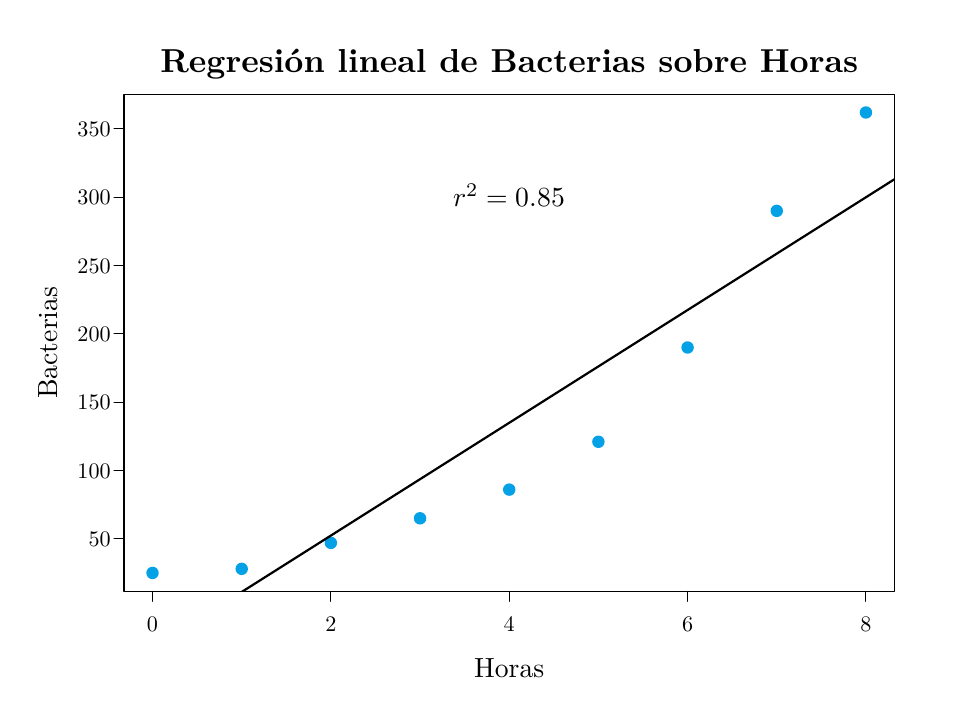
\begin{tikzpicture}[x=1pt,y=1pt]
\definecolor{fillColor}{RGB}{255,255,255}
\path[use as bounding box,fill=fillColor,fill opacity=0.00] (0,0) rectangle (325.21,238.49);
\begin{scope}
\path[clip] ( 34.80, 34.80) rectangle (313.21,214.49);
\definecolor{fillColor}{RGB}{5,161,230}

\path[fill=fillColor] ( 45.11, 41.46) circle (  2.25);

\path[fill=fillColor] ( 77.34, 42.94) circle (  2.25);

\path[fill=fillColor] (109.56, 52.32) circle (  2.25);

\path[fill=fillColor] (141.78, 61.20) circle (  2.25);

\path[fill=fillColor] (174.01, 71.57) circle (  2.25);

\path[fill=fillColor] (206.23, 88.85) circle (  2.25);

\path[fill=fillColor] (238.46,122.92) circle (  2.25);

\path[fill=fillColor] (270.68,172.29) circle (  2.25);

\path[fill=fillColor] (302.90,207.84) circle (  2.25);
\end{scope}
\begin{scope}
\path[clip] (  0.00,  0.00) rectangle (325.21,238.49);
\definecolor{drawColor}{RGB}{0,0,0}

\path[draw=drawColor,line width= 0.4pt,line join=round,line cap=round] ( 45.11, 34.80) -- (302.90, 34.80);

\path[draw=drawColor,line width= 0.4pt,line join=round,line cap=round] ( 45.11, 34.80) -- ( 45.11, 31.21);

\path[draw=drawColor,line width= 0.4pt,line join=round,line cap=round] (109.56, 34.80) -- (109.56, 31.21);

\path[draw=drawColor,line width= 0.4pt,line join=round,line cap=round] (174.01, 34.80) -- (174.01, 31.21);

\path[draw=drawColor,line width= 0.4pt,line join=round,line cap=round] (238.46, 34.80) -- (238.46, 31.21);

\path[draw=drawColor,line width= 0.4pt,line join=round,line cap=round] (302.90, 34.80) -- (302.90, 31.21);

\node[text=drawColor,anchor=base,inner sep=0pt, outer sep=0pt, scale=  0.80] at ( 45.11, 20.40) {0};

\node[text=drawColor,anchor=base,inner sep=0pt, outer sep=0pt, scale=  0.80] at (109.56, 20.40) {2};

\node[text=drawColor,anchor=base,inner sep=0pt, outer sep=0pt, scale=  0.80] at (174.01, 20.40) {4};

\node[text=drawColor,anchor=base,inner sep=0pt, outer sep=0pt, scale=  0.80] at (238.46, 20.40) {6};

\node[text=drawColor,anchor=base,inner sep=0pt, outer sep=0pt, scale=  0.80] at (302.90, 20.40) {8};

\path[draw=drawColor,line width= 0.4pt,line join=round,line cap=round] ( 34.80, 53.80) -- ( 34.80,201.91);

\path[draw=drawColor,line width= 0.4pt,line join=round,line cap=round] ( 34.80, 53.80) -- ( 31.21, 53.80);

\path[draw=drawColor,line width= 0.4pt,line join=round,line cap=round] ( 34.80, 78.48) -- ( 31.21, 78.48);

\path[draw=drawColor,line width= 0.4pt,line join=round,line cap=round] ( 34.80,103.17) -- ( 31.21,103.17);

\path[draw=drawColor,line width= 0.4pt,line join=round,line cap=round] ( 34.80,127.85) -- ( 31.21,127.85);

\path[draw=drawColor,line width= 0.4pt,line join=round,line cap=round] ( 34.80,152.54) -- ( 31.21,152.54);

\path[draw=drawColor,line width= 0.4pt,line join=round,line cap=round] ( 34.80,177.23) -- ( 31.21,177.23);

\path[draw=drawColor,line width= 0.4pt,line join=round,line cap=round] ( 34.80,201.91) -- ( 31.21,201.91);

\node[text=drawColor,anchor=base east,inner sep=0pt, outer sep=0pt, scale=  0.80] at ( 30.00, 51.04) {50};

\node[text=drawColor,anchor=base east,inner sep=0pt, outer sep=0pt, scale=  0.80] at ( 30.00, 75.73) {100};

\node[text=drawColor,anchor=base east,inner sep=0pt, outer sep=0pt, scale=  0.80] at ( 30.00,100.41) {150};

\node[text=drawColor,anchor=base east,inner sep=0pt, outer sep=0pt, scale=  0.80] at ( 30.00,125.10) {200};

\node[text=drawColor,anchor=base east,inner sep=0pt, outer sep=0pt, scale=  0.80] at ( 30.00,149.78) {250};

\node[text=drawColor,anchor=base east,inner sep=0pt, outer sep=0pt, scale=  0.80] at ( 30.00,174.47) {300};

\node[text=drawColor,anchor=base east,inner sep=0pt, outer sep=0pt, scale=  0.80] at ( 30.00,199.16) {350};

\path[draw=drawColor,line width= 0.4pt,line join=round,line cap=round] ( 34.80, 34.80) --
	(313.21, 34.80) --
	(313.21,214.49) --
	( 34.80,214.49) --
	( 34.80, 34.80);
\end{scope}
\begin{scope}
\path[clip] (  0.00,  0.00) rectangle (325.21,238.49);
\definecolor{drawColor}{RGB}{0,0,0}

\node[text=drawColor,anchor=base,inner sep=0pt, outer sep=0pt, scale=  1.20] at (174.01,222.30) {\bfseries Regresión lineal de Bacterias sobre Horas};

\node[text=drawColor,anchor=base,inner sep=0pt, outer sep=0pt, scale=  1.00] at (174.01,  3.60) {Horas};

\node[text=drawColor,rotate= 90.00,anchor=base,inner sep=0pt, outer sep=0pt, scale=  1.00] at ( 10.80,124.65) {Bacterias};
\end{scope}
\begin{scope}
\path[clip] ( 34.80, 34.80) rectangle (313.21,214.49);
\definecolor{drawColor}{RGB}{0,0,0}

\path[draw=drawColor,line width= 0.8pt,line join=round,line cap=round] ( 34.80,  7.69) -- (313.21,183.72);

\node[text=drawColor,anchor=base,inner sep=0pt, outer sep=0pt, scale=  1.00] at (174.01,173.76) {$r^2=0.85$};
\end{scope}
\end{tikzpicture}
}}
\mode<presentation>{\resizebox{0.9\textwidth}{!}{% Created by tikzDevice version 0.10.1 on 2016-02-27 13:16:26
% !TEX encoding = UTF-8 Unicode
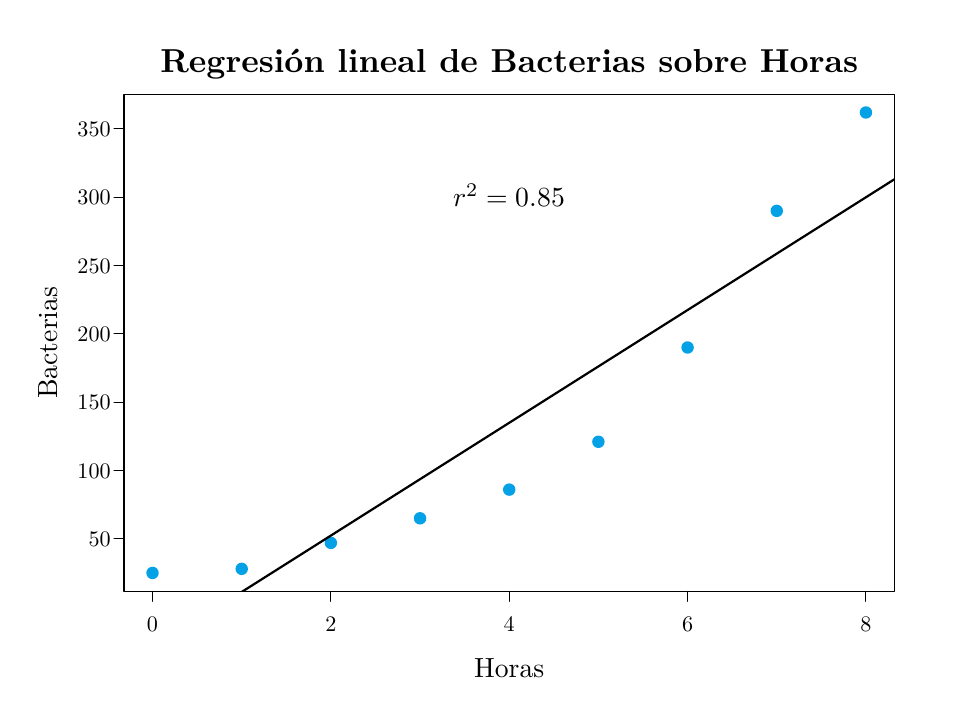
\begin{tikzpicture}[x=1pt,y=1pt]
\definecolor{fillColor}{RGB}{255,255,255}
\path[use as bounding box,fill=fillColor,fill opacity=0.00] (0,0) rectangle (325.21,238.49);
\begin{scope}
\path[clip] ( 34.80, 34.80) rectangle (313.21,214.49);
\definecolor{fillColor}{RGB}{5,161,230}

\path[fill=fillColor] ( 45.11, 41.46) circle (  2.25);

\path[fill=fillColor] ( 77.34, 42.94) circle (  2.25);

\path[fill=fillColor] (109.56, 52.32) circle (  2.25);

\path[fill=fillColor] (141.78, 61.20) circle (  2.25);

\path[fill=fillColor] (174.01, 71.57) circle (  2.25);

\path[fill=fillColor] (206.23, 88.85) circle (  2.25);

\path[fill=fillColor] (238.46,122.92) circle (  2.25);

\path[fill=fillColor] (270.68,172.29) circle (  2.25);

\path[fill=fillColor] (302.90,207.84) circle (  2.25);
\end{scope}
\begin{scope}
\path[clip] (  0.00,  0.00) rectangle (325.21,238.49);
\definecolor{drawColor}{RGB}{0,0,0}

\path[draw=drawColor,line width= 0.4pt,line join=round,line cap=round] ( 45.11, 34.80) -- (302.90, 34.80);

\path[draw=drawColor,line width= 0.4pt,line join=round,line cap=round] ( 45.11, 34.80) -- ( 45.11, 31.21);

\path[draw=drawColor,line width= 0.4pt,line join=round,line cap=round] (109.56, 34.80) -- (109.56, 31.21);

\path[draw=drawColor,line width= 0.4pt,line join=round,line cap=round] (174.01, 34.80) -- (174.01, 31.21);

\path[draw=drawColor,line width= 0.4pt,line join=round,line cap=round] (238.46, 34.80) -- (238.46, 31.21);

\path[draw=drawColor,line width= 0.4pt,line join=round,line cap=round] (302.90, 34.80) -- (302.90, 31.21);

\node[text=drawColor,anchor=base,inner sep=0pt, outer sep=0pt, scale=  0.80] at ( 45.11, 20.40) {0};

\node[text=drawColor,anchor=base,inner sep=0pt, outer sep=0pt, scale=  0.80] at (109.56, 20.40) {2};

\node[text=drawColor,anchor=base,inner sep=0pt, outer sep=0pt, scale=  0.80] at (174.01, 20.40) {4};

\node[text=drawColor,anchor=base,inner sep=0pt, outer sep=0pt, scale=  0.80] at (238.46, 20.40) {6};

\node[text=drawColor,anchor=base,inner sep=0pt, outer sep=0pt, scale=  0.80] at (302.90, 20.40) {8};

\path[draw=drawColor,line width= 0.4pt,line join=round,line cap=round] ( 34.80, 53.80) -- ( 34.80,201.91);

\path[draw=drawColor,line width= 0.4pt,line join=round,line cap=round] ( 34.80, 53.80) -- ( 31.21, 53.80);

\path[draw=drawColor,line width= 0.4pt,line join=round,line cap=round] ( 34.80, 78.48) -- ( 31.21, 78.48);

\path[draw=drawColor,line width= 0.4pt,line join=round,line cap=round] ( 34.80,103.17) -- ( 31.21,103.17);

\path[draw=drawColor,line width= 0.4pt,line join=round,line cap=round] ( 34.80,127.85) -- ( 31.21,127.85);

\path[draw=drawColor,line width= 0.4pt,line join=round,line cap=round] ( 34.80,152.54) -- ( 31.21,152.54);

\path[draw=drawColor,line width= 0.4pt,line join=round,line cap=round] ( 34.80,177.23) -- ( 31.21,177.23);

\path[draw=drawColor,line width= 0.4pt,line join=round,line cap=round] ( 34.80,201.91) -- ( 31.21,201.91);

\node[text=drawColor,anchor=base east,inner sep=0pt, outer sep=0pt, scale=  0.80] at ( 30.00, 51.04) {50};

\node[text=drawColor,anchor=base east,inner sep=0pt, outer sep=0pt, scale=  0.80] at ( 30.00, 75.73) {100};

\node[text=drawColor,anchor=base east,inner sep=0pt, outer sep=0pt, scale=  0.80] at ( 30.00,100.41) {150};

\node[text=drawColor,anchor=base east,inner sep=0pt, outer sep=0pt, scale=  0.80] at ( 30.00,125.10) {200};

\node[text=drawColor,anchor=base east,inner sep=0pt, outer sep=0pt, scale=  0.80] at ( 30.00,149.78) {250};

\node[text=drawColor,anchor=base east,inner sep=0pt, outer sep=0pt, scale=  0.80] at ( 30.00,174.47) {300};

\node[text=drawColor,anchor=base east,inner sep=0pt, outer sep=0pt, scale=  0.80] at ( 30.00,199.16) {350};

\path[draw=drawColor,line width= 0.4pt,line join=round,line cap=round] ( 34.80, 34.80) --
	(313.21, 34.80) --
	(313.21,214.49) --
	( 34.80,214.49) --
	( 34.80, 34.80);
\end{scope}
\begin{scope}
\path[clip] (  0.00,  0.00) rectangle (325.21,238.49);
\definecolor{drawColor}{RGB}{0,0,0}

\node[text=drawColor,anchor=base,inner sep=0pt, outer sep=0pt, scale=  1.20] at (174.01,222.30) {\bfseries Regresión lineal de Bacterias sobre Horas};

\node[text=drawColor,anchor=base,inner sep=0pt, outer sep=0pt, scale=  1.00] at (174.01,  3.60) {Horas};

\node[text=drawColor,rotate= 90.00,anchor=base,inner sep=0pt, outer sep=0pt, scale=  1.00] at ( 10.80,124.65) {Bacterias};
\end{scope}
\begin{scope}
\path[clip] ( 34.80, 34.80) rectangle (313.21,214.49);
\definecolor{drawColor}{RGB}{0,0,0}

\path[draw=drawColor,line width= 0.8pt,line join=round,line cap=round] ( 34.80,  7.69) -- (313.21,183.72);

\node[text=drawColor,anchor=base,inner sep=0pt, outer sep=0pt, scale=  1.00] at (174.01,173.76) {$r^2=0.85$};
\end{scope}
\end{tikzpicture}
}}
\end{center}
\end{column}
\end{columns}
\begin{center}
\emph{¿Es un buen modelo?}
\end{center}

\note{Si se calcula la recta de regresión del número de bacterias sobre las horas transcurridas, se observa que no es un mal modelo ya que
su coefiente de determinación lineal vale $0.85$. Ahora bien, que sea un buen modelo, no quiere decir que sea el mejor.
}
\end{frame}


%---------------------------------------------------------------------slide----
\begin{frame}
\frametitle{Ajuste de un modelo de regresión exponencial}
\framesubtitle{Evolución del número de bacterias de un cultivo}
Aunque el modelo lineal no es malo, de acuerdo al diagrama de dispersión es más lógico construir un modelo exponencial o cuadrático.

Para construir el modelo exponencial $y = ae^{bx}$ hay que realizar la transformación $z=\log y$, es decir, aplicar el logaritmo a la variable dependiente.

\begin{columns}
\begin{column}{0.45\textwidth}
\[
\begin{array}{c|c|c}
\mbox{Horas} & \mbox{Bacterias} & \mbox{Log Bacterias}\\
\hline
0 &  25 & 3.22\\
1 & 28 & 3.33\\
2 &  47 & 3.85\\
3 & 65  & 4.17\\
4 & 86 & 4.45\\
5 & 121 & 4.80\\
6 & 190 & 5.25\\
7 & 290 & 5.67\\
8 & 362 & 5.89
\end{array}
\]
\end{column}
\begin{column}{0.55\textwidth}
\begin{center}
\tikzsetnextfilename{regresion/evolucion_log_bacterias}
\mode<article>{\resizebox{0.7\textwidth}{!}{% Created by tikzDevice version 0.10.1 on 2016-02-27 13:16:44
% !TEX encoding = UTF-8 Unicode
\begin{tikzpicture}[x=1pt,y=1pt]
\definecolor{fillColor}{RGB}{255,255,255}
\path[use as bounding box,fill=fillColor,fill opacity=0.00] (0,0) rectangle (325.21,238.49);
\begin{scope}
\path[clip] ( 34.80, 34.80) rectangle (313.21,214.49);
\definecolor{fillColor}{RGB}{5,161,230}

\path[fill=fillColor] ( 45.11, 41.46) circle (  2.25);

\path[fill=fillColor] ( 77.34, 48.51) circle (  2.25);

\path[fill=fillColor] (109.56, 80.75) circle (  2.25);

\path[fill=fillColor] (141.78,100.94) circle (  2.25);

\path[fill=fillColor] (174.01,118.36) circle (  2.25);

\path[fill=fillColor] (206.23,139.62) circle (  2.25);

\path[fill=fillColor] (238.46,167.71) circle (  2.25);

\path[fill=fillColor] (270.68,194.03) circle (  2.25);

\path[fill=fillColor] (302.90,207.84) circle (  2.25);
\end{scope}
\begin{scope}
\path[clip] (  0.00,  0.00) rectangle (325.21,238.49);
\definecolor{drawColor}{RGB}{0,0,0}

\path[draw=drawColor,line width= 0.4pt,line join=round,line cap=round] ( 45.11, 34.80) -- (302.90, 34.80);

\path[draw=drawColor,line width= 0.4pt,line join=round,line cap=round] ( 45.11, 34.80) -- ( 45.11, 31.21);

\path[draw=drawColor,line width= 0.4pt,line join=round,line cap=round] (109.56, 34.80) -- (109.56, 31.21);

\path[draw=drawColor,line width= 0.4pt,line join=round,line cap=round] (174.01, 34.80) -- (174.01, 31.21);

\path[draw=drawColor,line width= 0.4pt,line join=round,line cap=round] (238.46, 34.80) -- (238.46, 31.21);

\path[draw=drawColor,line width= 0.4pt,line join=round,line cap=round] (302.90, 34.80) -- (302.90, 31.21);

\node[text=drawColor,anchor=base,inner sep=0pt, outer sep=0pt, scale=  0.80] at ( 45.11, 20.40) {0};

\node[text=drawColor,anchor=base,inner sep=0pt, outer sep=0pt, scale=  0.80] at (109.56, 20.40) {2};

\node[text=drawColor,anchor=base,inner sep=0pt, outer sep=0pt, scale=  0.80] at (174.01, 20.40) {4};

\node[text=drawColor,anchor=base,inner sep=0pt, outer sep=0pt, scale=  0.80] at (238.46, 20.40) {6};

\node[text=drawColor,anchor=base,inner sep=0pt, outer sep=0pt, scale=  0.80] at (302.90, 20.40) {8};

\path[draw=drawColor,line width= 0.4pt,line join=round,line cap=round] ( 34.80, 58.96) -- ( 34.80,183.46);

\path[draw=drawColor,line width= 0.4pt,line join=round,line cap=round] ( 34.80, 58.96) -- ( 31.21, 58.96);

\path[draw=drawColor,line width= 0.4pt,line join=round,line cap=round] ( 34.80, 90.08) -- ( 31.21, 90.08);

\path[draw=drawColor,line width= 0.4pt,line join=round,line cap=round] ( 34.80,121.21) -- ( 31.21,121.21);

\path[draw=drawColor,line width= 0.4pt,line join=round,line cap=round] ( 34.80,152.33) -- ( 31.21,152.33);

\path[draw=drawColor,line width= 0.4pt,line join=round,line cap=round] ( 34.80,183.46) -- ( 31.21,183.46);

\node[text=drawColor,anchor=base east,inner sep=0pt, outer sep=0pt, scale=  0.80] at ( 30.00, 56.20) {3.5};

\node[text=drawColor,anchor=base east,inner sep=0pt, outer sep=0pt, scale=  0.80] at ( 30.00, 87.32) {4.0};

\node[text=drawColor,anchor=base east,inner sep=0pt, outer sep=0pt, scale=  0.80] at ( 30.00,118.45) {4.5};

\node[text=drawColor,anchor=base east,inner sep=0pt, outer sep=0pt, scale=  0.80] at ( 30.00,149.58) {5.0};

\node[text=drawColor,anchor=base east,inner sep=0pt, outer sep=0pt, scale=  0.80] at ( 30.00,180.70) {5.5};

\path[draw=drawColor,line width= 0.4pt,line join=round,line cap=round] ( 34.80, 34.80) --
	(313.21, 34.80) --
	(313.21,214.49) --
	( 34.80,214.49) --
	( 34.80, 34.80);
\end{scope}
\begin{scope}
\path[clip] (  0.00,  0.00) rectangle (325.21,238.49);
\definecolor{drawColor}{RGB}{0,0,0}

\node[text=drawColor,anchor=base,inner sep=0pt, outer sep=0pt, scale=  1.20] at (174.01,222.30) {\bfseries Evolución de $\log$(Bacterias)};

\node[text=drawColor,anchor=base,inner sep=0pt, outer sep=0pt, scale=  1.00] at (174.01,  3.60) {Horas};

\node[text=drawColor,rotate= 90.00,anchor=base,inner sep=0pt, outer sep=0pt, scale=  1.00] at ( 10.80,124.65) {$\log$(Bacterias)};
\end{scope}
\end{tikzpicture}
}}
\mode<presentation>{\resizebox{0.9\textwidth}{!}{% Created by tikzDevice version 0.10.1 on 2016-02-27 13:16:44
% !TEX encoding = UTF-8 Unicode
\begin{tikzpicture}[x=1pt,y=1pt]
\definecolor{fillColor}{RGB}{255,255,255}
\path[use as bounding box,fill=fillColor,fill opacity=0.00] (0,0) rectangle (325.21,238.49);
\begin{scope}
\path[clip] ( 34.80, 34.80) rectangle (313.21,214.49);
\definecolor{fillColor}{RGB}{5,161,230}

\path[fill=fillColor] ( 45.11, 41.46) circle (  2.25);

\path[fill=fillColor] ( 77.34, 48.51) circle (  2.25);

\path[fill=fillColor] (109.56, 80.75) circle (  2.25);

\path[fill=fillColor] (141.78,100.94) circle (  2.25);

\path[fill=fillColor] (174.01,118.36) circle (  2.25);

\path[fill=fillColor] (206.23,139.62) circle (  2.25);

\path[fill=fillColor] (238.46,167.71) circle (  2.25);

\path[fill=fillColor] (270.68,194.03) circle (  2.25);

\path[fill=fillColor] (302.90,207.84) circle (  2.25);
\end{scope}
\begin{scope}
\path[clip] (  0.00,  0.00) rectangle (325.21,238.49);
\definecolor{drawColor}{RGB}{0,0,0}

\path[draw=drawColor,line width= 0.4pt,line join=round,line cap=round] ( 45.11, 34.80) -- (302.90, 34.80);

\path[draw=drawColor,line width= 0.4pt,line join=round,line cap=round] ( 45.11, 34.80) -- ( 45.11, 31.21);

\path[draw=drawColor,line width= 0.4pt,line join=round,line cap=round] (109.56, 34.80) -- (109.56, 31.21);

\path[draw=drawColor,line width= 0.4pt,line join=round,line cap=round] (174.01, 34.80) -- (174.01, 31.21);

\path[draw=drawColor,line width= 0.4pt,line join=round,line cap=round] (238.46, 34.80) -- (238.46, 31.21);

\path[draw=drawColor,line width= 0.4pt,line join=round,line cap=round] (302.90, 34.80) -- (302.90, 31.21);

\node[text=drawColor,anchor=base,inner sep=0pt, outer sep=0pt, scale=  0.80] at ( 45.11, 20.40) {0};

\node[text=drawColor,anchor=base,inner sep=0pt, outer sep=0pt, scale=  0.80] at (109.56, 20.40) {2};

\node[text=drawColor,anchor=base,inner sep=0pt, outer sep=0pt, scale=  0.80] at (174.01, 20.40) {4};

\node[text=drawColor,anchor=base,inner sep=0pt, outer sep=0pt, scale=  0.80] at (238.46, 20.40) {6};

\node[text=drawColor,anchor=base,inner sep=0pt, outer sep=0pt, scale=  0.80] at (302.90, 20.40) {8};

\path[draw=drawColor,line width= 0.4pt,line join=round,line cap=round] ( 34.80, 58.96) -- ( 34.80,183.46);

\path[draw=drawColor,line width= 0.4pt,line join=round,line cap=round] ( 34.80, 58.96) -- ( 31.21, 58.96);

\path[draw=drawColor,line width= 0.4pt,line join=round,line cap=round] ( 34.80, 90.08) -- ( 31.21, 90.08);

\path[draw=drawColor,line width= 0.4pt,line join=round,line cap=round] ( 34.80,121.21) -- ( 31.21,121.21);

\path[draw=drawColor,line width= 0.4pt,line join=round,line cap=round] ( 34.80,152.33) -- ( 31.21,152.33);

\path[draw=drawColor,line width= 0.4pt,line join=round,line cap=round] ( 34.80,183.46) -- ( 31.21,183.46);

\node[text=drawColor,anchor=base east,inner sep=0pt, outer sep=0pt, scale=  0.80] at ( 30.00, 56.20) {3.5};

\node[text=drawColor,anchor=base east,inner sep=0pt, outer sep=0pt, scale=  0.80] at ( 30.00, 87.32) {4.0};

\node[text=drawColor,anchor=base east,inner sep=0pt, outer sep=0pt, scale=  0.80] at ( 30.00,118.45) {4.5};

\node[text=drawColor,anchor=base east,inner sep=0pt, outer sep=0pt, scale=  0.80] at ( 30.00,149.58) {5.0};

\node[text=drawColor,anchor=base east,inner sep=0pt, outer sep=0pt, scale=  0.80] at ( 30.00,180.70) {5.5};

\path[draw=drawColor,line width= 0.4pt,line join=round,line cap=round] ( 34.80, 34.80) --
	(313.21, 34.80) --
	(313.21,214.49) --
	( 34.80,214.49) --
	( 34.80, 34.80);
\end{scope}
\begin{scope}
\path[clip] (  0.00,  0.00) rectangle (325.21,238.49);
\definecolor{drawColor}{RGB}{0,0,0}

\node[text=drawColor,anchor=base,inner sep=0pt, outer sep=0pt, scale=  1.20] at (174.01,222.30) {\bfseries Evolución de $\log$(Bacterias)};

\node[text=drawColor,anchor=base,inner sep=0pt, outer sep=0pt, scale=  1.00] at (174.01,  3.60) {Horas};

\node[text=drawColor,rotate= 90.00,anchor=base,inner sep=0pt, outer sep=0pt, scale=  1.00] at ( 10.80,124.65) {$\log$(Bacterias)};
\end{scope}
\end{tikzpicture}
}}
\end{center}
\end{column}
\end{columns}

\note{Para construir el modelo de regresión exponencial hay que aplicar el logaritmo neperiano a la variable dependiente, que en este caso
es el número de bacterias. El logaritmo neperiano de 25 nos da 3.22, el de 28 nos da 3.33 y así sucesivamente, de manera que obtenemos una
nueva variable que es el logarítmo de las bacterias. 

Si representamos el diagrama de dispersion del logaritmo de las bacterias y las horas transcurridas, podemos comprobar cómo ahora la nube de
puntos tiene forma lineal, es decir, mediante la transformación logarítmica de la variable dependiente hemos convertido una relación
exponencial en una relación lineal.
}
\end{frame}


%---------------------------------------------------------------------slide----
\begin{frame}
\frametitle{Ajuste de un modelo de regresión exponencial}
\framesubtitle{Evolución del número de bacterias de un cultivo}
Ahora sólo queda calcular la recta de regresión del logaritmo de Bacterias sobre Horas
\begin{columns}
\begin{column}{0.45\textwidth}
\[
\mbox{Log Bacterias} = 3.107 + 0.352\, \mbox{Horas}.
\]
Y deshaciendo el cambio de variable, se obtiene el modelo exponencial
\[
\mbox{Bacterias} = e^{3.107+0.352\,\textrm{Horas}}, \mbox{ con } r^2=0.99.
\]
Como se puede apreciar, el modelo exponencial se ajusta mucho mejor que el modelo lineal.
\end{column}
\begin{column}{0.55\textwidth}
\begin{center}
\tikzsetnextfilename{regresion/regresion_exponencial_bacterias}
\mode<article>{\resizebox{0.7\textwidth}{!}{% Created by tikzDevice version 0.10.1 on 2016-02-27 13:16:47
% !TEX encoding = UTF-8 Unicode
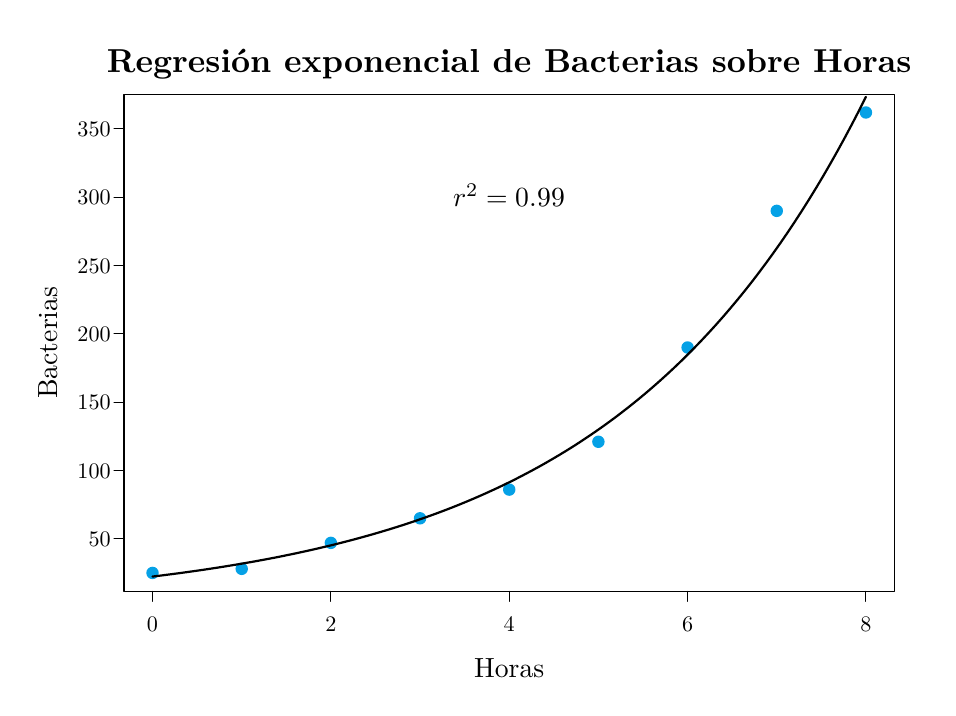
\begin{tikzpicture}[x=1pt,y=1pt]
\definecolor{fillColor}{RGB}{255,255,255}
\path[use as bounding box,fill=fillColor,fill opacity=0.00] (0,0) rectangle (325.21,238.49);
\begin{scope}
\path[clip] ( 34.80, 34.80) rectangle (313.21,214.49);
\definecolor{fillColor}{RGB}{5,161,230}

\path[fill=fillColor] ( 45.11, 41.46) circle (  2.25);

\path[fill=fillColor] ( 77.34, 42.94) circle (  2.25);

\path[fill=fillColor] (109.56, 52.32) circle (  2.25);

\path[fill=fillColor] (141.78, 61.20) circle (  2.25);

\path[fill=fillColor] (174.01, 71.57) circle (  2.25);

\path[fill=fillColor] (206.23, 88.85) circle (  2.25);

\path[fill=fillColor] (238.46,122.92) circle (  2.25);

\path[fill=fillColor] (270.68,172.29) circle (  2.25);

\path[fill=fillColor] (302.90,207.84) circle (  2.25);
\end{scope}
\begin{scope}
\path[clip] (  0.00,  0.00) rectangle (325.21,238.49);
\definecolor{drawColor}{RGB}{0,0,0}

\path[draw=drawColor,line width= 0.4pt,line join=round,line cap=round] ( 45.11, 34.80) -- (302.90, 34.80);

\path[draw=drawColor,line width= 0.4pt,line join=round,line cap=round] ( 45.11, 34.80) -- ( 45.11, 31.21);

\path[draw=drawColor,line width= 0.4pt,line join=round,line cap=round] (109.56, 34.80) -- (109.56, 31.21);

\path[draw=drawColor,line width= 0.4pt,line join=round,line cap=round] (174.01, 34.80) -- (174.01, 31.21);

\path[draw=drawColor,line width= 0.4pt,line join=round,line cap=round] (238.46, 34.80) -- (238.46, 31.21);

\path[draw=drawColor,line width= 0.4pt,line join=round,line cap=round] (302.90, 34.80) -- (302.90, 31.21);

\node[text=drawColor,anchor=base,inner sep=0pt, outer sep=0pt, scale=  0.80] at ( 45.11, 20.40) {0};

\node[text=drawColor,anchor=base,inner sep=0pt, outer sep=0pt, scale=  0.80] at (109.56, 20.40) {2};

\node[text=drawColor,anchor=base,inner sep=0pt, outer sep=0pt, scale=  0.80] at (174.01, 20.40) {4};

\node[text=drawColor,anchor=base,inner sep=0pt, outer sep=0pt, scale=  0.80] at (238.46, 20.40) {6};

\node[text=drawColor,anchor=base,inner sep=0pt, outer sep=0pt, scale=  0.80] at (302.90, 20.40) {8};

\path[draw=drawColor,line width= 0.4pt,line join=round,line cap=round] ( 34.80, 53.80) -- ( 34.80,201.91);

\path[draw=drawColor,line width= 0.4pt,line join=round,line cap=round] ( 34.80, 53.80) -- ( 31.21, 53.80);

\path[draw=drawColor,line width= 0.4pt,line join=round,line cap=round] ( 34.80, 78.48) -- ( 31.21, 78.48);

\path[draw=drawColor,line width= 0.4pt,line join=round,line cap=round] ( 34.80,103.17) -- ( 31.21,103.17);

\path[draw=drawColor,line width= 0.4pt,line join=round,line cap=round] ( 34.80,127.85) -- ( 31.21,127.85);

\path[draw=drawColor,line width= 0.4pt,line join=round,line cap=round] ( 34.80,152.54) -- ( 31.21,152.54);

\path[draw=drawColor,line width= 0.4pt,line join=round,line cap=round] ( 34.80,177.23) -- ( 31.21,177.23);

\path[draw=drawColor,line width= 0.4pt,line join=round,line cap=round] ( 34.80,201.91) -- ( 31.21,201.91);

\node[text=drawColor,anchor=base east,inner sep=0pt, outer sep=0pt, scale=  0.80] at ( 30.00, 51.04) {50};

\node[text=drawColor,anchor=base east,inner sep=0pt, outer sep=0pt, scale=  0.80] at ( 30.00, 75.73) {100};

\node[text=drawColor,anchor=base east,inner sep=0pt, outer sep=0pt, scale=  0.80] at ( 30.00,100.41) {150};

\node[text=drawColor,anchor=base east,inner sep=0pt, outer sep=0pt, scale=  0.80] at ( 30.00,125.10) {200};

\node[text=drawColor,anchor=base east,inner sep=0pt, outer sep=0pt, scale=  0.80] at ( 30.00,149.78) {250};

\node[text=drawColor,anchor=base east,inner sep=0pt, outer sep=0pt, scale=  0.80] at ( 30.00,174.47) {300};

\node[text=drawColor,anchor=base east,inner sep=0pt, outer sep=0pt, scale=  0.80] at ( 30.00,199.16) {350};

\path[draw=drawColor,line width= 0.4pt,line join=round,line cap=round] ( 34.80, 34.80) --
	(313.21, 34.80) --
	(313.21,214.49) --
	( 34.80,214.49) --
	( 34.80, 34.80);
\end{scope}
\begin{scope}
\path[clip] (  0.00,  0.00) rectangle (325.21,238.49);
\definecolor{drawColor}{RGB}{0,0,0}

\node[text=drawColor,anchor=base,inner sep=0pt, outer sep=0pt, scale=  1.20] at (174.01,222.30) {\bfseries Regresión exponencial de Bacterias sobre Horas};

\node[text=drawColor,anchor=base,inner sep=0pt, outer sep=0pt, scale=  1.00] at (174.01,  3.60) {Horas};

\node[text=drawColor,rotate= 90.00,anchor=base,inner sep=0pt, outer sep=0pt, scale=  1.00] at ( 10.80,124.65) {Bacterias};
\end{scope}
\begin{scope}
\path[clip] ( 34.80, 34.80) rectangle (313.21,214.49);
\definecolor{drawColor}{RGB}{0,0,0}

\path[draw=drawColor,line width= 0.8pt,line join=round,line cap=round] ( 45.11, 40.15) --
	( 47.69, 40.46) --
	( 50.27, 40.79) --
	( 52.85, 41.12) --
	( 55.42, 41.46) --
	( 58.00, 41.82) --
	( 60.58, 42.18) --
	( 63.16, 42.55) --
	( 65.73, 42.94) --
	( 68.31, 43.33) --
	( 70.89, 43.74) --
	( 73.47, 44.16) --
	( 76.05, 44.59) --
	( 78.62, 45.03) --
	( 81.20, 45.48) --
	( 83.78, 45.95) --
	( 86.36, 46.43) --
	( 88.94, 46.92) --
	( 91.51, 47.43) --
	( 94.09, 47.96) --
	( 96.67, 48.49) --
	( 99.25, 49.05) --
	(101.83, 49.62) --
	(104.40, 50.20) --
	(106.98, 50.81) --
	(109.56, 51.42) --
	(112.14, 52.06) --
	(114.72, 52.72) --
	(117.29, 53.39) --
	(119.87, 54.09) --
	(122.45, 54.80) --
	(125.03, 55.53) --
	(127.60, 56.29) --
	(130.18, 57.06) --
	(132.76, 57.86) --
	(135.34, 58.68) --
	(137.92, 59.53) --
	(140.49, 60.39) --
	(143.07, 61.29) --
	(145.65, 62.21) --
	(148.23, 63.15) --
	(150.81, 64.12) --
	(153.38, 65.12) --
	(155.96, 66.15) --
	(158.54, 67.21) --
	(161.12, 68.30) --
	(163.70, 69.42) --
	(166.27, 70.57) --
	(168.85, 71.75) --
	(171.43, 72.97) --
	(174.01, 74.22) --
	(176.59, 75.51) --
	(179.16, 76.84) --
	(181.74, 78.20) --
	(184.32, 79.60) --
	(186.90, 81.04) --
	(189.47, 82.53) --
	(192.05, 84.05) --
	(194.63, 85.62) --
	(197.21, 87.23) --
	(199.79, 88.89) --
	(202.36, 90.60) --
	(204.94, 92.36) --
	(207.52, 94.16) --
	(210.10, 96.02) --
	(212.68, 97.93) --
	(215.25, 99.90) --
	(217.83,101.92) --
	(220.41,104.00) --
	(222.99,106.14) --
	(225.57,108.34) --
	(228.14,110.60) --
	(230.72,112.93) --
	(233.30,115.32) --
	(235.88,117.78) --
	(238.46,120.32) --
	(241.03,122.92) --
	(243.61,125.60) --
	(246.19,128.36) --
	(248.77,131.19) --
	(251.34,134.10) --
	(253.92,137.10) --
	(256.50,140.19) --
	(259.08,143.36) --
	(261.66,146.62) --
	(264.23,149.98) --
	(266.81,153.43) --
	(269.39,156.98) --
	(271.97,160.63) --
	(274.55,164.39) --
	(277.12,168.25) --
	(279.70,172.23) --
	(282.28,176.31) --
	(284.86,180.52) --
	(287.44,184.84) --
	(290.01,189.29) --
	(292.59,193.86) --
	(295.17,198.57) --
	(297.75,203.41) --
	(300.33,208.39) --
	(302.90,213.51);

\node[text=drawColor,anchor=base,inner sep=0pt, outer sep=0pt, scale=  1.00] at (174.01,173.76) {$r^2=0.99$};
\end{scope}
\end{tikzpicture}
}}
\mode<presentation>{\resizebox{0.9\textwidth}{!}{% Created by tikzDevice version 0.10.1 on 2016-02-27 13:16:47
% !TEX encoding = UTF-8 Unicode
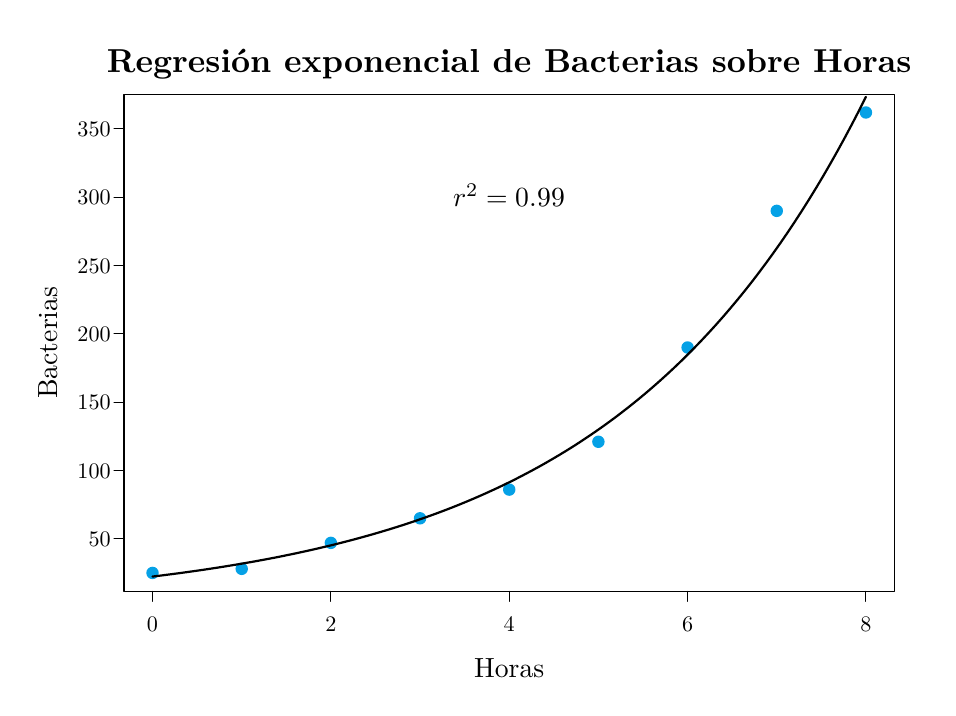
\begin{tikzpicture}[x=1pt,y=1pt]
\definecolor{fillColor}{RGB}{255,255,255}
\path[use as bounding box,fill=fillColor,fill opacity=0.00] (0,0) rectangle (325.21,238.49);
\begin{scope}
\path[clip] ( 34.80, 34.80) rectangle (313.21,214.49);
\definecolor{fillColor}{RGB}{5,161,230}

\path[fill=fillColor] ( 45.11, 41.46) circle (  2.25);

\path[fill=fillColor] ( 77.34, 42.94) circle (  2.25);

\path[fill=fillColor] (109.56, 52.32) circle (  2.25);

\path[fill=fillColor] (141.78, 61.20) circle (  2.25);

\path[fill=fillColor] (174.01, 71.57) circle (  2.25);

\path[fill=fillColor] (206.23, 88.85) circle (  2.25);

\path[fill=fillColor] (238.46,122.92) circle (  2.25);

\path[fill=fillColor] (270.68,172.29) circle (  2.25);

\path[fill=fillColor] (302.90,207.84) circle (  2.25);
\end{scope}
\begin{scope}
\path[clip] (  0.00,  0.00) rectangle (325.21,238.49);
\definecolor{drawColor}{RGB}{0,0,0}

\path[draw=drawColor,line width= 0.4pt,line join=round,line cap=round] ( 45.11, 34.80) -- (302.90, 34.80);

\path[draw=drawColor,line width= 0.4pt,line join=round,line cap=round] ( 45.11, 34.80) -- ( 45.11, 31.21);

\path[draw=drawColor,line width= 0.4pt,line join=round,line cap=round] (109.56, 34.80) -- (109.56, 31.21);

\path[draw=drawColor,line width= 0.4pt,line join=round,line cap=round] (174.01, 34.80) -- (174.01, 31.21);

\path[draw=drawColor,line width= 0.4pt,line join=round,line cap=round] (238.46, 34.80) -- (238.46, 31.21);

\path[draw=drawColor,line width= 0.4pt,line join=round,line cap=round] (302.90, 34.80) -- (302.90, 31.21);

\node[text=drawColor,anchor=base,inner sep=0pt, outer sep=0pt, scale=  0.80] at ( 45.11, 20.40) {0};

\node[text=drawColor,anchor=base,inner sep=0pt, outer sep=0pt, scale=  0.80] at (109.56, 20.40) {2};

\node[text=drawColor,anchor=base,inner sep=0pt, outer sep=0pt, scale=  0.80] at (174.01, 20.40) {4};

\node[text=drawColor,anchor=base,inner sep=0pt, outer sep=0pt, scale=  0.80] at (238.46, 20.40) {6};

\node[text=drawColor,anchor=base,inner sep=0pt, outer sep=0pt, scale=  0.80] at (302.90, 20.40) {8};

\path[draw=drawColor,line width= 0.4pt,line join=round,line cap=round] ( 34.80, 53.80) -- ( 34.80,201.91);

\path[draw=drawColor,line width= 0.4pt,line join=round,line cap=round] ( 34.80, 53.80) -- ( 31.21, 53.80);

\path[draw=drawColor,line width= 0.4pt,line join=round,line cap=round] ( 34.80, 78.48) -- ( 31.21, 78.48);

\path[draw=drawColor,line width= 0.4pt,line join=round,line cap=round] ( 34.80,103.17) -- ( 31.21,103.17);

\path[draw=drawColor,line width= 0.4pt,line join=round,line cap=round] ( 34.80,127.85) -- ( 31.21,127.85);

\path[draw=drawColor,line width= 0.4pt,line join=round,line cap=round] ( 34.80,152.54) -- ( 31.21,152.54);

\path[draw=drawColor,line width= 0.4pt,line join=round,line cap=round] ( 34.80,177.23) -- ( 31.21,177.23);

\path[draw=drawColor,line width= 0.4pt,line join=round,line cap=round] ( 34.80,201.91) -- ( 31.21,201.91);

\node[text=drawColor,anchor=base east,inner sep=0pt, outer sep=0pt, scale=  0.80] at ( 30.00, 51.04) {50};

\node[text=drawColor,anchor=base east,inner sep=0pt, outer sep=0pt, scale=  0.80] at ( 30.00, 75.73) {100};

\node[text=drawColor,anchor=base east,inner sep=0pt, outer sep=0pt, scale=  0.80] at ( 30.00,100.41) {150};

\node[text=drawColor,anchor=base east,inner sep=0pt, outer sep=0pt, scale=  0.80] at ( 30.00,125.10) {200};

\node[text=drawColor,anchor=base east,inner sep=0pt, outer sep=0pt, scale=  0.80] at ( 30.00,149.78) {250};

\node[text=drawColor,anchor=base east,inner sep=0pt, outer sep=0pt, scale=  0.80] at ( 30.00,174.47) {300};

\node[text=drawColor,anchor=base east,inner sep=0pt, outer sep=0pt, scale=  0.80] at ( 30.00,199.16) {350};

\path[draw=drawColor,line width= 0.4pt,line join=round,line cap=round] ( 34.80, 34.80) --
	(313.21, 34.80) --
	(313.21,214.49) --
	( 34.80,214.49) --
	( 34.80, 34.80);
\end{scope}
\begin{scope}
\path[clip] (  0.00,  0.00) rectangle (325.21,238.49);
\definecolor{drawColor}{RGB}{0,0,0}

\node[text=drawColor,anchor=base,inner sep=0pt, outer sep=0pt, scale=  1.20] at (174.01,222.30) {\bfseries Regresión exponencial de Bacterias sobre Horas};

\node[text=drawColor,anchor=base,inner sep=0pt, outer sep=0pt, scale=  1.00] at (174.01,  3.60) {Horas};

\node[text=drawColor,rotate= 90.00,anchor=base,inner sep=0pt, outer sep=0pt, scale=  1.00] at ( 10.80,124.65) {Bacterias};
\end{scope}
\begin{scope}
\path[clip] ( 34.80, 34.80) rectangle (313.21,214.49);
\definecolor{drawColor}{RGB}{0,0,0}

\path[draw=drawColor,line width= 0.8pt,line join=round,line cap=round] ( 45.11, 40.15) --
	( 47.69, 40.46) --
	( 50.27, 40.79) --
	( 52.85, 41.12) --
	( 55.42, 41.46) --
	( 58.00, 41.82) --
	( 60.58, 42.18) --
	( 63.16, 42.55) --
	( 65.73, 42.94) --
	( 68.31, 43.33) --
	( 70.89, 43.74) --
	( 73.47, 44.16) --
	( 76.05, 44.59) --
	( 78.62, 45.03) --
	( 81.20, 45.48) --
	( 83.78, 45.95) --
	( 86.36, 46.43) --
	( 88.94, 46.92) --
	( 91.51, 47.43) --
	( 94.09, 47.96) --
	( 96.67, 48.49) --
	( 99.25, 49.05) --
	(101.83, 49.62) --
	(104.40, 50.20) --
	(106.98, 50.81) --
	(109.56, 51.42) --
	(112.14, 52.06) --
	(114.72, 52.72) --
	(117.29, 53.39) --
	(119.87, 54.09) --
	(122.45, 54.80) --
	(125.03, 55.53) --
	(127.60, 56.29) --
	(130.18, 57.06) --
	(132.76, 57.86) --
	(135.34, 58.68) --
	(137.92, 59.53) --
	(140.49, 60.39) --
	(143.07, 61.29) --
	(145.65, 62.21) --
	(148.23, 63.15) --
	(150.81, 64.12) --
	(153.38, 65.12) --
	(155.96, 66.15) --
	(158.54, 67.21) --
	(161.12, 68.30) --
	(163.70, 69.42) --
	(166.27, 70.57) --
	(168.85, 71.75) --
	(171.43, 72.97) --
	(174.01, 74.22) --
	(176.59, 75.51) --
	(179.16, 76.84) --
	(181.74, 78.20) --
	(184.32, 79.60) --
	(186.90, 81.04) --
	(189.47, 82.53) --
	(192.05, 84.05) --
	(194.63, 85.62) --
	(197.21, 87.23) --
	(199.79, 88.89) --
	(202.36, 90.60) --
	(204.94, 92.36) --
	(207.52, 94.16) --
	(210.10, 96.02) --
	(212.68, 97.93) --
	(215.25, 99.90) --
	(217.83,101.92) --
	(220.41,104.00) --
	(222.99,106.14) --
	(225.57,108.34) --
	(228.14,110.60) --
	(230.72,112.93) --
	(233.30,115.32) --
	(235.88,117.78) --
	(238.46,120.32) --
	(241.03,122.92) --
	(243.61,125.60) --
	(246.19,128.36) --
	(248.77,131.19) --
	(251.34,134.10) --
	(253.92,137.10) --
	(256.50,140.19) --
	(259.08,143.36) --
	(261.66,146.62) --
	(264.23,149.98) --
	(266.81,153.43) --
	(269.39,156.98) --
	(271.97,160.63) --
	(274.55,164.39) --
	(277.12,168.25) --
	(279.70,172.23) --
	(282.28,176.31) --
	(284.86,180.52) --
	(287.44,184.84) --
	(290.01,189.29) --
	(292.59,193.86) --
	(295.17,198.57) --
	(297.75,203.41) --
	(300.33,208.39) --
	(302.90,213.51);

\node[text=drawColor,anchor=base,inner sep=0pt, outer sep=0pt, scale=  1.00] at (174.01,173.76) {$r^2=0.99$};
\end{scope}
\end{tikzpicture}
}}
\end{center}
\end{column}
\end{columns}

\note{Si ahora calculamos la recta de regresión del logaritmo de las bacterias sobre las horas, se tiene $\mbox{Log Bacterias} = 3.107 +
0.352\, \mbox{Horas}$, cuyo coeficiente de determinación lineal vale $0.99$, lo cual indica un ajuste casi perfecto de la recta. 

Finalmente, para obtener el modelo exponencial, basta con desacer la transformación logarítmica del número de bacterias, aplicando la
función exponencial, lo que nos da $\mbox{Bacterias} = e^{3.107+0.352\,\textrm{Horas}}$, y cuyo coeficiente de determinación exponencial
coincide con el de la recta anterior, de manera que se puede concluir que el modelo exponencial explica muyo mejor la relación entre el
número de bacterias y las horas que el modelo lineal. }
\end{frame}


\subsection{Riesgos de la regresión}
%---------------------------------------------------------------------slide----
\begin{frame}
\frametitle{Interpretación de un coeficiente de determinación pequeño}
Es importante señalar que cada modelo de regresión tiene su propio coeficiente de determinación.
Así, un coeficiente de determinación cercano a cero significa que no existe relación entre las variables del tipo planteado por el modelo, pero \emph{eso no quiere decir que las variables sean
independientes}, ya que puede existir relación de otro tipo.
\begin{center}
\tikzsetnextfilename{regresion/regresion_lineal_relacion_cuadratica}
\resizebox{0.49\textwidth}{!}{% Created by tikzDevice version 0.10.1 on 2016-02-27 13:23:43
% !TEX encoding = UTF-8 Unicode
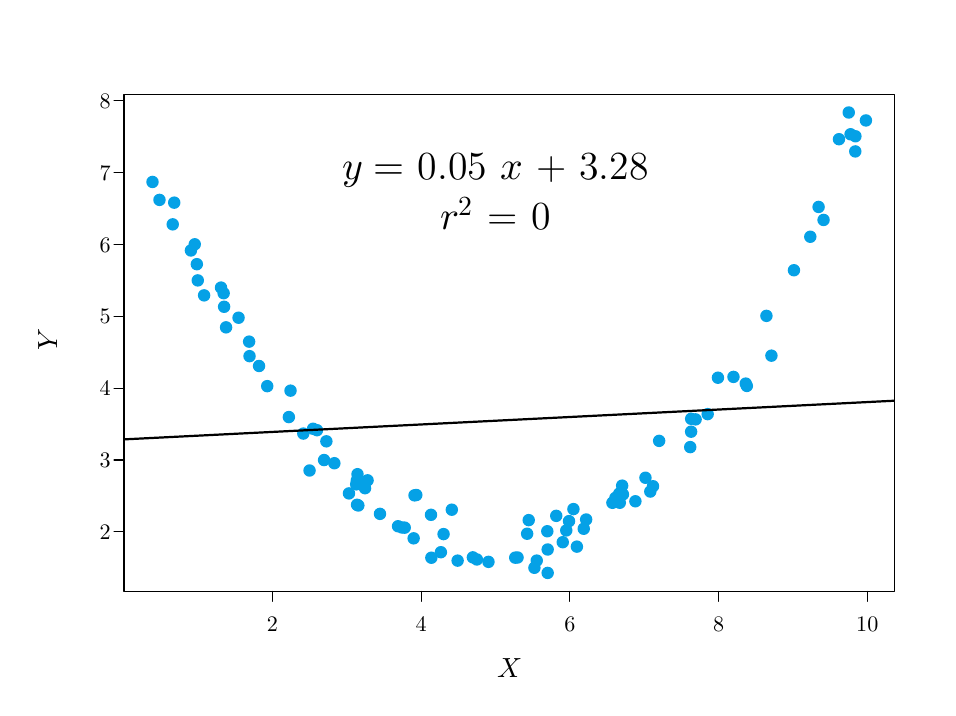
\begin{tikzpicture}[x=1pt,y=1pt]
\definecolor{fillColor}{RGB}{255,255,255}
\path[use as bounding box,fill=fillColor,fill opacity=0.00] (0,0) rectangle (325.21,238.49);
\begin{scope}
\path[clip] ( 34.80, 34.80) rectangle (313.21,214.49);
\definecolor{fillColor}{RGB}{5,161,230}

\path[fill=fillColor] ( 58.99,157.98) circle (  2.25);

\path[fill=fillColor] (139.47, 53.96) circle (  2.25);

\path[fill=fillColor] (297.34,199.97) circle (  2.25);

\path[fill=fillColor] (282.80,162.94) circle (  2.25);

\path[fill=fillColor] (119.48, 65.83) circle (  2.25);

\path[fill=fillColor] (287.59,169.01) circle (  2.25);

\path[fill=fillColor] (241.36, 96.94) circle (  2.25);

\path[fill=fillColor] (135.27, 57.88) circle (  2.25);

\path[fill=fillColor] (104.54, 93.04) circle (  2.25);

\path[fill=fillColor] (239.73, 92.50) circle (  2.25);

\path[fill=fillColor] (249.43,112.00) circle (  2.25);

\path[fill=fillColor] (195.62, 60.18) circle (  2.25);

\path[fill=fillColor] (119.18, 77.13) circle (  2.25);

\path[fill=fillColor] ( 83.60,116.24) circle (  2.25);

\path[fill=fillColor] (103.13, 93.56) circle (  2.25);

\path[fill=fillColor] (116.10, 70.20) circle (  2.25);

\path[fill=fillColor] (166.50, 45.46) circle (  2.25);

\path[fill=fillColor] (107.93, 89.02) circle (  2.25);

\path[fill=fillColor] (127.31, 62.80) circle (  2.25);

\path[fill=fillColor] (160.87, 47.09) circle (  2.25);

\path[fill=fillColor] ( 52.41,167.42) circle (  2.25);

\path[fill=fillColor] (201.81, 60.77) circle (  2.25);

\path[fill=fillColor] ( 61.13,153.03) circle (  2.25);

\path[fill=fillColor] (145.87, 46.96) circle (  2.25);

\path[fill=fillColor] (296.69,207.84) circle (  2.25);

\path[fill=fillColor] ( 52.95,175.26) circle (  2.25);

\path[fill=fillColor] (255.03,112.30) circle (  2.25);

\path[fill=fillColor] ( 69.87,144.57) circle (  2.25);

\path[fill=fillColor] ( 45.11,182.74) circle (  2.25);

\path[fill=fillColor] ( 70.81,142.54) circle (  2.25);

\path[fill=fillColor] (285.80,173.71) circle (  2.25);

\path[fill=fillColor] (239.41, 86.93) circle (  2.25);

\path[fill=fillColor] (213.96, 66.81) circle (  2.25);

\path[fill=fillColor] (122.82, 74.92) circle (  2.25);

\path[fill=fillColor] (187.90, 41.46) circle (  2.25);

\path[fill=fillColor] (118.71, 73.47) circle (  2.25);

\path[fill=fillColor] (183.95, 45.92) circle (  2.25);

\path[fill=fillColor] (194.62, 56.82) circle (  2.25);

\path[fill=fillColor] (153.26, 64.31) circle (  2.25);

\path[fill=fillColor] (119.02, 66.08) circle (  2.25);

\path[fill=fillColor] (145.74, 62.46) circle (  2.25);

\path[fill=fillColor] ( 70.98,137.64) circle (  2.25);

\path[fill=fillColor] (110.82, 81.11) circle (  2.25);

\path[fill=fillColor] (215.10, 69.84) circle (  2.25);

\path[fill=fillColor] (259.87,109.04) circle (  2.25);

\path[fill=fillColor] (191.00, 62.09) circle (  2.25);

\path[fill=fillColor] (155.36, 45.90) circle (  2.25);

\path[fill=fillColor] (214.81, 73.00) circle (  2.25);

\path[fill=fillColor] ( 63.75,141.76) circle (  2.25);

\path[fill=fillColor] (139.78, 69.49) circle (  2.25);

\path[fill=fillColor] (176.18, 46.98) circle (  2.25);

\path[fill=fillColor] (133.84, 58.33) circle (  2.25);

\path[fill=fillColor] (211.29, 66.80) circle (  2.25);

\path[fill=fillColor] (293.16,198.18) circle (  2.25);

\path[fill=fillColor] (177.01, 47.03) circle (  2.25);

\path[fill=fillColor] (181.05, 60.54) circle (  2.25);

\path[fill=fillColor] (150.28, 55.49) circle (  2.25);

\path[fill=fillColor] ( 61.47,147.17) circle (  2.25);

\path[fill=fillColor] (213.75, 70.13) circle (  2.25);

\path[fill=fillColor] ( 80.02,125.04) circle (  2.25);

\path[fill=fillColor] (193.35, 52.56) circle (  2.25);

\path[fill=fillColor] (187.90, 49.93) circle (  2.25);

\path[fill=fillColor] ( 71.69,130.20) circle (  2.25);

\path[fill=fillColor] (183.11, 43.32) circle (  2.25);

\path[fill=fillColor] ( 47.63,176.26) circle (  2.25);

\path[fill=fillColor] (200.93, 57.43) circle (  2.25);

\path[fill=fillColor] ( 94.98,107.32) circle (  2.25);

\path[fill=fillColor] (140.43, 69.62) circle (  2.25);

\path[fill=fillColor] (136.24, 57.82) circle (  2.25);

\path[fill=fillColor] ( 60.37,160.21) circle (  2.25);

\path[fill=fillColor] (225.96, 72.79) circle (  2.25);

\path[fill=fillColor] (266.95,134.35) circle (  2.25);

\path[fill=fillColor] ( 94.38, 97.78) circle (  2.25);

\path[fill=fillColor] ( 99.60, 91.82) circle (  2.25);

\path[fill=fillColor] (149.31, 48.94) circle (  2.25);

\path[fill=fillColor] ( 86.56,108.95) circle (  2.25);

\path[fill=fillColor] (107.10, 82.25) circle (  2.25);

\path[fill=fillColor] (101.86, 78.47) circle (  2.25);

\path[fill=fillColor] (224.98, 70.87) circle (  2.25);

\path[fill=fillColor] (121.91, 72.08) circle (  2.25);

\path[fill=fillColor] (212.38, 68.58) circle (  2.25);

\path[fill=fillColor] (239.75, 97.16) circle (  2.25);

\path[fill=fillColor] (228.18, 89.18) circle (  2.25);

\path[fill=fillColor] ( 80.17,119.79) circle (  2.25);

\path[fill=fillColor] (197.21, 64.53) circle (  2.25);

\path[fill=fillColor] (259.47,109.88) circle (  2.25);

\path[fill=fillColor] (245.71, 98.85) circle (  2.25);

\path[fill=fillColor] (162.32, 46.32) circle (  2.25);

\path[fill=fillColor] (302.90,204.96) circle (  2.25);

\path[fill=fillColor] (299.05,193.77) circle (  2.25);

\path[fill=fillColor] (276.89,150.83) circle (  2.25);

\path[fill=fillColor] (118.93, 74.87) circle (  2.25);

\path[fill=fillColor] (299.10,199.25) circle (  2.25);

\path[fill=fillColor] (198.46, 50.96) circle (  2.25);

\path[fill=fillColor] (180.48, 55.62) circle (  2.25);

\path[fill=fillColor] ( 76.20,133.68) circle (  2.25);

\path[fill=fillColor] (223.23, 75.85) circle (  2.25);

\path[fill=fillColor] (268.75,119.97) circle (  2.25);

\path[fill=fillColor] (219.60, 67.35) circle (  2.25);

\path[fill=fillColor] (187.77, 56.52) circle (  2.25);
\end{scope}
\begin{scope}
\path[clip] (  0.00,  0.00) rectangle (325.21,238.49);
\definecolor{drawColor}{RGB}{0,0,0}

\path[draw=drawColor,line width= 0.4pt,line join=round,line cap=round] ( 88.41, 34.80) -- (303.39, 34.80);

\path[draw=drawColor,line width= 0.4pt,line join=round,line cap=round] ( 88.41, 34.80) -- ( 88.41, 31.21);

\path[draw=drawColor,line width= 0.4pt,line join=round,line cap=round] (142.16, 34.80) -- (142.16, 31.21);

\path[draw=drawColor,line width= 0.4pt,line join=round,line cap=round] (195.90, 34.80) -- (195.90, 31.21);

\path[draw=drawColor,line width= 0.4pt,line join=round,line cap=round] (249.65, 34.80) -- (249.65, 31.21);

\path[draw=drawColor,line width= 0.4pt,line join=round,line cap=round] (303.39, 34.80) -- (303.39, 31.21);

\node[text=drawColor,anchor=base,inner sep=0pt, outer sep=0pt, scale=  0.80] at ( 88.41, 20.40) {2};

\node[text=drawColor,anchor=base,inner sep=0pt, outer sep=0pt, scale=  0.80] at (142.16, 20.40) {4};

\node[text=drawColor,anchor=base,inner sep=0pt, outer sep=0pt, scale=  0.80] at (195.90, 20.40) {6};

\node[text=drawColor,anchor=base,inner sep=0pt, outer sep=0pt, scale=  0.80] at (249.65, 20.40) {8};

\node[text=drawColor,anchor=base,inner sep=0pt, outer sep=0pt, scale=  0.80] at (303.39, 20.40) {10};

\path[draw=drawColor,line width= 0.4pt,line join=round,line cap=round] ( 34.80, 56.32) -- ( 34.80,212.09);

\path[draw=drawColor,line width= 0.4pt,line join=round,line cap=round] ( 34.80, 56.32) -- ( 31.21, 56.32);

\path[draw=drawColor,line width= 0.4pt,line join=round,line cap=round] ( 34.80, 82.28) -- ( 31.21, 82.28);

\path[draw=drawColor,line width= 0.4pt,line join=round,line cap=round] ( 34.80,108.25) -- ( 31.21,108.25);

\path[draw=drawColor,line width= 0.4pt,line join=round,line cap=round] ( 34.80,134.21) -- ( 31.21,134.21);

\path[draw=drawColor,line width= 0.4pt,line join=round,line cap=round] ( 34.80,160.17) -- ( 31.21,160.17);

\path[draw=drawColor,line width= 0.4pt,line join=round,line cap=round] ( 34.80,186.13) -- ( 31.21,186.13);

\path[draw=drawColor,line width= 0.4pt,line join=round,line cap=round] ( 34.80,212.09) -- ( 31.21,212.09);

\node[text=drawColor,anchor=base east,inner sep=0pt, outer sep=0pt, scale=  0.80] at ( 30.00, 53.57) {2};

\node[text=drawColor,anchor=base east,inner sep=0pt, outer sep=0pt, scale=  0.80] at ( 30.00, 79.53) {3};

\node[text=drawColor,anchor=base east,inner sep=0pt, outer sep=0pt, scale=  0.80] at ( 30.00,105.49) {4};

\node[text=drawColor,anchor=base east,inner sep=0pt, outer sep=0pt, scale=  0.80] at ( 30.00,131.45) {5};

\node[text=drawColor,anchor=base east,inner sep=0pt, outer sep=0pt, scale=  0.80] at ( 30.00,157.41) {6};

\node[text=drawColor,anchor=base east,inner sep=0pt, outer sep=0pt, scale=  0.80] at ( 30.00,183.37) {7};

\node[text=drawColor,anchor=base east,inner sep=0pt, outer sep=0pt, scale=  0.80] at ( 30.00,209.33) {8};

\path[draw=drawColor,line width= 0.4pt,line join=round,line cap=round] ( 34.80, 34.80) --
	(313.21, 34.80) --
	(313.21,214.49) --
	( 34.80,214.49) --
	( 34.80, 34.80);
\end{scope}
\begin{scope}
\path[clip] (  0.00,  0.00) rectangle (325.21,238.49);
\definecolor{drawColor}{RGB}{0,0,0}

\node[text=drawColor,anchor=base,inner sep=0pt, outer sep=0pt, scale=  1.00] at (174.01,  3.60) {$X$};

\node[text=drawColor,rotate= 90.00,anchor=base,inner sep=0pt, outer sep=0pt, scale=  1.00] at ( 10.80,124.65) {$Y$};
\end{scope}
\begin{scope}
\path[clip] ( 34.80, 34.80) rectangle (313.21,214.49);
\definecolor{drawColor}{RGB}{0,0,0}

\path[draw=drawColor,line width= 0.8pt,line join=round,line cap=round] ( 34.80, 89.72) -- (313.21,103.69);

\node[text=drawColor,anchor=base,inner sep=0pt, outer sep=0pt, scale=  1.00] at (169.03,183.63) {\Large $y=$ 0.05 $x$ + 3.28};

\node[text=drawColor,anchor=base,inner sep=0pt, outer sep=0pt, scale=  1.00] at (169.03,165.45) {\Large $r^2$ = 0};
\end{scope}
\end{tikzpicture}
}
\tikzsetnextfilename{regresion/regresion_cuadratica}
\resizebox{0.49\textwidth}{!}{% Created by tikzDevice version 0.10.1 on 2016-02-27 13:23:44
% !TEX encoding = UTF-8 Unicode
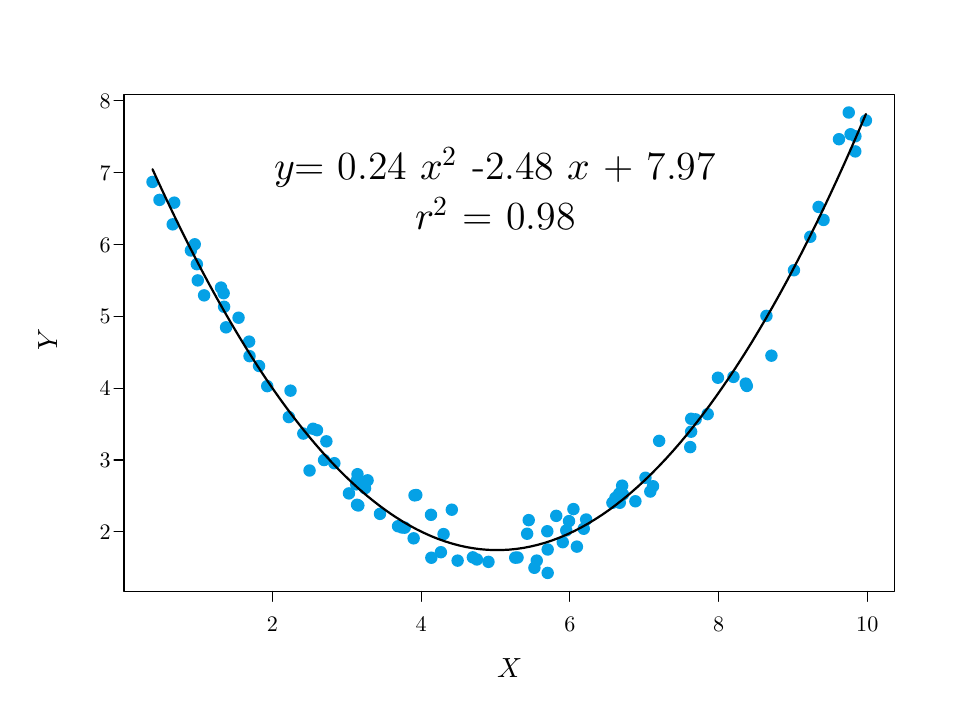
\begin{tikzpicture}[x=1pt,y=1pt]
\definecolor{fillColor}{RGB}{255,255,255}
\path[use as bounding box,fill=fillColor,fill opacity=0.00] (0,0) rectangle (325.21,238.49);
\begin{scope}
\path[clip] ( 34.80, 34.80) rectangle (313.21,214.49);
\definecolor{fillColor}{RGB}{5,161,230}

\path[fill=fillColor] ( 58.99,157.98) circle (  2.25);

\path[fill=fillColor] (139.47, 53.96) circle (  2.25);

\path[fill=fillColor] (297.34,199.97) circle (  2.25);

\path[fill=fillColor] (282.80,162.94) circle (  2.25);

\path[fill=fillColor] (119.48, 65.83) circle (  2.25);

\path[fill=fillColor] (287.59,169.01) circle (  2.25);

\path[fill=fillColor] (241.36, 96.94) circle (  2.25);

\path[fill=fillColor] (135.27, 57.88) circle (  2.25);

\path[fill=fillColor] (104.54, 93.04) circle (  2.25);

\path[fill=fillColor] (239.73, 92.50) circle (  2.25);

\path[fill=fillColor] (249.43,112.00) circle (  2.25);

\path[fill=fillColor] (195.62, 60.18) circle (  2.25);

\path[fill=fillColor] (119.18, 77.13) circle (  2.25);

\path[fill=fillColor] ( 83.60,116.24) circle (  2.25);

\path[fill=fillColor] (103.13, 93.56) circle (  2.25);

\path[fill=fillColor] (116.10, 70.20) circle (  2.25);

\path[fill=fillColor] (166.50, 45.46) circle (  2.25);

\path[fill=fillColor] (107.93, 89.02) circle (  2.25);

\path[fill=fillColor] (127.31, 62.80) circle (  2.25);

\path[fill=fillColor] (160.87, 47.09) circle (  2.25);

\path[fill=fillColor] ( 52.41,167.42) circle (  2.25);

\path[fill=fillColor] (201.81, 60.77) circle (  2.25);

\path[fill=fillColor] ( 61.13,153.03) circle (  2.25);

\path[fill=fillColor] (145.87, 46.96) circle (  2.25);

\path[fill=fillColor] (296.69,207.84) circle (  2.25);

\path[fill=fillColor] ( 52.95,175.26) circle (  2.25);

\path[fill=fillColor] (255.03,112.30) circle (  2.25);

\path[fill=fillColor] ( 69.87,144.57) circle (  2.25);

\path[fill=fillColor] ( 45.11,182.74) circle (  2.25);

\path[fill=fillColor] ( 70.81,142.54) circle (  2.25);

\path[fill=fillColor] (285.80,173.71) circle (  2.25);

\path[fill=fillColor] (239.41, 86.93) circle (  2.25);

\path[fill=fillColor] (213.96, 66.81) circle (  2.25);

\path[fill=fillColor] (122.82, 74.92) circle (  2.25);

\path[fill=fillColor] (187.90, 41.46) circle (  2.25);

\path[fill=fillColor] (118.71, 73.47) circle (  2.25);

\path[fill=fillColor] (183.95, 45.92) circle (  2.25);

\path[fill=fillColor] (194.62, 56.82) circle (  2.25);

\path[fill=fillColor] (153.26, 64.31) circle (  2.25);

\path[fill=fillColor] (119.02, 66.08) circle (  2.25);

\path[fill=fillColor] (145.74, 62.46) circle (  2.25);

\path[fill=fillColor] ( 70.98,137.64) circle (  2.25);

\path[fill=fillColor] (110.82, 81.11) circle (  2.25);

\path[fill=fillColor] (215.10, 69.84) circle (  2.25);

\path[fill=fillColor] (259.87,109.04) circle (  2.25);

\path[fill=fillColor] (191.00, 62.09) circle (  2.25);

\path[fill=fillColor] (155.36, 45.90) circle (  2.25);

\path[fill=fillColor] (214.81, 73.00) circle (  2.25);

\path[fill=fillColor] ( 63.75,141.76) circle (  2.25);

\path[fill=fillColor] (139.78, 69.49) circle (  2.25);

\path[fill=fillColor] (176.18, 46.98) circle (  2.25);

\path[fill=fillColor] (133.84, 58.33) circle (  2.25);

\path[fill=fillColor] (211.29, 66.80) circle (  2.25);

\path[fill=fillColor] (293.16,198.18) circle (  2.25);

\path[fill=fillColor] (177.01, 47.03) circle (  2.25);

\path[fill=fillColor] (181.05, 60.54) circle (  2.25);

\path[fill=fillColor] (150.28, 55.49) circle (  2.25);

\path[fill=fillColor] ( 61.47,147.17) circle (  2.25);

\path[fill=fillColor] (213.75, 70.13) circle (  2.25);

\path[fill=fillColor] ( 80.02,125.04) circle (  2.25);

\path[fill=fillColor] (193.35, 52.56) circle (  2.25);

\path[fill=fillColor] (187.90, 49.93) circle (  2.25);

\path[fill=fillColor] ( 71.69,130.20) circle (  2.25);

\path[fill=fillColor] (183.11, 43.32) circle (  2.25);

\path[fill=fillColor] ( 47.63,176.26) circle (  2.25);

\path[fill=fillColor] (200.93, 57.43) circle (  2.25);

\path[fill=fillColor] ( 94.98,107.32) circle (  2.25);

\path[fill=fillColor] (140.43, 69.62) circle (  2.25);

\path[fill=fillColor] (136.24, 57.82) circle (  2.25);

\path[fill=fillColor] ( 60.37,160.21) circle (  2.25);

\path[fill=fillColor] (225.96, 72.79) circle (  2.25);

\path[fill=fillColor] (266.95,134.35) circle (  2.25);

\path[fill=fillColor] ( 94.38, 97.78) circle (  2.25);

\path[fill=fillColor] ( 99.60, 91.82) circle (  2.25);

\path[fill=fillColor] (149.31, 48.94) circle (  2.25);

\path[fill=fillColor] ( 86.56,108.95) circle (  2.25);

\path[fill=fillColor] (107.10, 82.25) circle (  2.25);

\path[fill=fillColor] (101.86, 78.47) circle (  2.25);

\path[fill=fillColor] (224.98, 70.87) circle (  2.25);

\path[fill=fillColor] (121.91, 72.08) circle (  2.25);

\path[fill=fillColor] (212.38, 68.58) circle (  2.25);

\path[fill=fillColor] (239.75, 97.16) circle (  2.25);

\path[fill=fillColor] (228.18, 89.18) circle (  2.25);

\path[fill=fillColor] ( 80.17,119.79) circle (  2.25);

\path[fill=fillColor] (197.21, 64.53) circle (  2.25);

\path[fill=fillColor] (259.47,109.88) circle (  2.25);

\path[fill=fillColor] (245.71, 98.85) circle (  2.25);

\path[fill=fillColor] (162.32, 46.32) circle (  2.25);

\path[fill=fillColor] (302.90,204.96) circle (  2.25);

\path[fill=fillColor] (299.05,193.77) circle (  2.25);

\path[fill=fillColor] (276.89,150.83) circle (  2.25);

\path[fill=fillColor] (118.93, 74.87) circle (  2.25);

\path[fill=fillColor] (299.10,199.25) circle (  2.25);

\path[fill=fillColor] (198.46, 50.96) circle (  2.25);

\path[fill=fillColor] (180.48, 55.62) circle (  2.25);

\path[fill=fillColor] ( 76.20,133.68) circle (  2.25);

\path[fill=fillColor] (223.23, 75.85) circle (  2.25);

\path[fill=fillColor] (268.75,119.97) circle (  2.25);

\path[fill=fillColor] (219.60, 67.35) circle (  2.25);

\path[fill=fillColor] (187.77, 56.52) circle (  2.25);
\end{scope}
\begin{scope}
\path[clip] (  0.00,  0.00) rectangle (325.21,238.49);
\definecolor{drawColor}{RGB}{0,0,0}

\path[draw=drawColor,line width= 0.4pt,line join=round,line cap=round] ( 88.41, 34.80) -- (303.39, 34.80);

\path[draw=drawColor,line width= 0.4pt,line join=round,line cap=round] ( 88.41, 34.80) -- ( 88.41, 31.21);

\path[draw=drawColor,line width= 0.4pt,line join=round,line cap=round] (142.16, 34.80) -- (142.16, 31.21);

\path[draw=drawColor,line width= 0.4pt,line join=round,line cap=round] (195.90, 34.80) -- (195.90, 31.21);

\path[draw=drawColor,line width= 0.4pt,line join=round,line cap=round] (249.65, 34.80) -- (249.65, 31.21);

\path[draw=drawColor,line width= 0.4pt,line join=round,line cap=round] (303.39, 34.80) -- (303.39, 31.21);

\node[text=drawColor,anchor=base,inner sep=0pt, outer sep=0pt, scale=  0.80] at ( 88.41, 20.40) {2};

\node[text=drawColor,anchor=base,inner sep=0pt, outer sep=0pt, scale=  0.80] at (142.16, 20.40) {4};

\node[text=drawColor,anchor=base,inner sep=0pt, outer sep=0pt, scale=  0.80] at (195.90, 20.40) {6};

\node[text=drawColor,anchor=base,inner sep=0pt, outer sep=0pt, scale=  0.80] at (249.65, 20.40) {8};

\node[text=drawColor,anchor=base,inner sep=0pt, outer sep=0pt, scale=  0.80] at (303.39, 20.40) {10};

\path[draw=drawColor,line width= 0.4pt,line join=round,line cap=round] ( 34.80, 56.32) -- ( 34.80,212.09);

\path[draw=drawColor,line width= 0.4pt,line join=round,line cap=round] ( 34.80, 56.32) -- ( 31.21, 56.32);

\path[draw=drawColor,line width= 0.4pt,line join=round,line cap=round] ( 34.80, 82.28) -- ( 31.21, 82.28);

\path[draw=drawColor,line width= 0.4pt,line join=round,line cap=round] ( 34.80,108.25) -- ( 31.21,108.25);

\path[draw=drawColor,line width= 0.4pt,line join=round,line cap=round] ( 34.80,134.21) -- ( 31.21,134.21);

\path[draw=drawColor,line width= 0.4pt,line join=round,line cap=round] ( 34.80,160.17) -- ( 31.21,160.17);

\path[draw=drawColor,line width= 0.4pt,line join=round,line cap=round] ( 34.80,186.13) -- ( 31.21,186.13);

\path[draw=drawColor,line width= 0.4pt,line join=round,line cap=round] ( 34.80,212.09) -- ( 31.21,212.09);

\node[text=drawColor,anchor=base east,inner sep=0pt, outer sep=0pt, scale=  0.80] at ( 30.00, 53.57) {2};

\node[text=drawColor,anchor=base east,inner sep=0pt, outer sep=0pt, scale=  0.80] at ( 30.00, 79.53) {3};

\node[text=drawColor,anchor=base east,inner sep=0pt, outer sep=0pt, scale=  0.80] at ( 30.00,105.49) {4};

\node[text=drawColor,anchor=base east,inner sep=0pt, outer sep=0pt, scale=  0.80] at ( 30.00,131.45) {5};

\node[text=drawColor,anchor=base east,inner sep=0pt, outer sep=0pt, scale=  0.80] at ( 30.00,157.41) {6};

\node[text=drawColor,anchor=base east,inner sep=0pt, outer sep=0pt, scale=  0.80] at ( 30.00,183.37) {7};

\node[text=drawColor,anchor=base east,inner sep=0pt, outer sep=0pt, scale=  0.80] at ( 30.00,209.33) {8};

\path[draw=drawColor,line width= 0.4pt,line join=round,line cap=round] ( 34.80, 34.80) --
	(313.21, 34.80) --
	(313.21,214.49) --
	( 34.80,214.49) --
	( 34.80, 34.80);
\end{scope}
\begin{scope}
\path[clip] (  0.00,  0.00) rectangle (325.21,238.49);
\definecolor{drawColor}{RGB}{0,0,0}

\node[text=drawColor,anchor=base,inner sep=0pt, outer sep=0pt, scale=  1.00] at (174.01,  3.60) {$X$};

\node[text=drawColor,rotate= 90.00,anchor=base,inner sep=0pt, outer sep=0pt, scale=  1.00] at ( 10.80,124.65) {$Y$};
\end{scope}
\begin{scope}
\path[clip] ( 34.80, 34.80) rectangle (313.21,214.49);
\definecolor{drawColor}{RGB}{0,0,0}

\path[draw=drawColor,line width= 0.8pt,line join=round,line cap=round] ( 45.11,187.33) --
	( 47.69,181.69) --
	( 50.27,176.17) --
	( 52.85,170.77) --
	( 55.42,165.48) --
	( 58.00,160.31) --
	( 60.58,155.27) --
	( 63.16,150.33) --
	( 65.73,145.52) --
	( 68.31,140.83) --
	( 70.89,136.25) --
	( 73.47,131.79) --
	( 76.05,127.45) --
	( 78.62,123.23) --
	( 81.20,119.12) --
	( 83.78,115.13) --
	( 86.36,111.26) --
	( 88.94,107.51) --
	( 91.51,103.88) --
	( 94.09,100.36) --
	( 96.67, 96.97) --
	( 99.25, 93.69) --
	(101.83, 90.52) --
	(104.40, 87.48) --
	(106.98, 84.55) --
	(109.56, 81.75) --
	(112.14, 79.06) --
	(114.72, 76.48) --
	(117.29, 74.03) --
	(119.87, 71.69) --
	(122.45, 69.48) --
	(125.03, 67.38) --
	(127.61, 65.39) --
	(130.18, 63.53) --
	(132.76, 61.78) --
	(135.34, 60.15) --
	(137.92, 58.64) --
	(140.49, 57.25) --
	(143.07, 55.98) --
	(145.65, 54.82) --
	(148.23, 53.78) --
	(150.81, 52.86) --
	(153.38, 52.06) --
	(155.96, 51.37) --
	(158.54, 50.80) --
	(161.12, 50.36) --
	(163.70, 50.02) --
	(166.27, 49.81) --
	(168.85, 49.72) --
	(171.43, 49.74) --
	(174.01, 49.88) --
	(176.59, 50.14) --
	(179.16, 50.51) --
	(181.74, 51.01) --
	(184.32, 51.62) --
	(186.90, 52.35) --
	(189.47, 53.20) --
	(192.05, 54.17) --
	(194.63, 55.25) --
	(197.21, 56.45) --
	(199.79, 57.77) --
	(202.36, 59.21) --
	(204.94, 60.77) --
	(207.52, 62.44) --
	(210.10, 64.23) --
	(212.68, 66.14) --
	(215.25, 68.17) --
	(217.83, 70.32) --
	(220.41, 72.58) --
	(222.99, 74.96) --
	(225.57, 77.46) --
	(228.14, 80.08) --
	(230.72, 82.81) --
	(233.30, 85.67) --
	(235.88, 88.64) --
	(238.46, 91.73) --
	(241.03, 94.94) --
	(243.61, 98.26) --
	(246.19,101.70) --
	(248.77,105.27) --
	(251.34,108.94) --
	(253.92,112.74) --
	(256.50,116.66) --
	(259.08,120.69) --
	(261.66,124.84) --
	(264.23,129.11) --
	(266.81,133.50) --
	(269.39,138.00) --
	(271.97,142.62) --
	(274.55,147.36) --
	(277.12,152.22) --
	(279.70,157.20) --
	(282.28,162.29) --
	(284.86,167.51) --
	(287.44,172.84) --
	(290.01,178.28) --
	(292.59,183.85) --
	(295.17,189.53) --
	(297.75,195.34) --
	(300.33,201.26) --
	(302.90,207.29);

\node[text=drawColor,anchor=base,inner sep=0pt, outer sep=0pt, scale=  1.00] at (169.03,183.63) {\Large $y$= 0.24 $x^2$ -2.48 $x$ + 7.97};

\node[text=drawColor,anchor=base,inner sep=0pt, outer sep=0pt, scale=  1.00] at (169.03,165.45) {\Large $r^2$ = 0.98};
\end{scope}
\end{tikzpicture}
}
\end{center}

\note{Hay que recordar que tanto el coeficiente de determinación hace referencia a un modelo concreto, de manera que
un coeficiente $r^2=0$ significa que no existe relación entre las variables del tipo planteado por el modelo, pero \emph{eso no quiere decir
que las variables sean independientes}, ya que puede existir relación de otro tipo.

En las gráficas puede apreciarse cómo al ajustar una recta sobre esta nube de puntos se obtiene un coeficiente de determinación
prácticamente nulo pero sin embargo hay una clara relación parabólica entre las variables, por lo que no podemos decir que las variables
son independientes, tan sólo que no tienen relación lineal.}
\end{frame}


%---------------------------------------------------------------------slide----
\begin{frame}
\frametitle{Datos atípicos en regresión}
Los \emph{datos atípicos} en un estudio de regresión son los puntos que claramente no siguen la tendencia del resto de los puntos en el diagrama de dispersión, incluso si los valores del par no se pueden considerar atípicos para cada variable por separado.

\begin{center}
\tikzsetnextfilename{regresion/diagrama_dispersion_con_datos_atipicos}
\resizebox{0.7\textwidth}{!}{% Created by tikzDevice version 0.10.1 on 2016-02-27 13:47:46
% !TEX encoding = UTF-8 Unicode
\begin{tikzpicture}[x=1pt,y=1pt]
\definecolor{fillColor}{RGB}{255,255,255}
\path[use as bounding box,fill=fillColor,fill opacity=0.00] (0,0) rectangle (325.21,238.49);
\begin{scope}
\path[clip] ( 34.80, 34.80) rectangle (313.21,214.49);
\definecolor{fillColor}{RGB}{5,161,230}

\path[fill=fillColor] ( 72.15,118.24) circle (  2.25);

\path[fill=fillColor] (270.97, 51.29) circle (  2.25);

\path[fill=fillColor] ( 93.12,103.19) circle (  2.25);

\path[fill=fillColor] (146.01, 92.94) circle (  2.25);

\path[fill=fillColor] (211.70, 67.10) circle (  2.25);

\path[fill=fillColor] (149.78, 92.94) circle (  2.25);

\path[fill=fillColor] (289.83, 43.74) circle (  2.25);

\path[fill=fillColor] (300.55, 44.55) circle (  2.25);

\path[fill=fillColor] (121.56, 97.84) circle (  2.25);

\path[fill=fillColor] (251.34,174.56) circle (  2.25);
\end{scope}
\begin{scope}
\path[clip] (  0.00,  0.00) rectangle (325.21,238.49);
\definecolor{drawColor}{RGB}{0,0,0}

\path[draw=drawColor,line width= 0.4pt,line join=round,line cap=round] ( 45.11, 34.80) -- (302.90, 34.80);

\path[draw=drawColor,line width= 0.4pt,line join=round,line cap=round] ( 45.11, 34.80) -- ( 45.11, 31.21);

\path[draw=drawColor,line width= 0.4pt,line join=round,line cap=round] ( 96.67, 34.80) -- ( 96.67, 31.21);

\path[draw=drawColor,line width= 0.4pt,line join=round,line cap=round] (148.23, 34.80) -- (148.23, 31.21);

\path[draw=drawColor,line width= 0.4pt,line join=round,line cap=round] (199.79, 34.80) -- (199.79, 31.21);

\path[draw=drawColor,line width= 0.4pt,line join=round,line cap=round] (251.34, 34.80) -- (251.34, 31.21);

\path[draw=drawColor,line width= 0.4pt,line join=round,line cap=round] (302.90, 34.80) -- (302.90, 31.21);

\node[text=drawColor,anchor=base,inner sep=0pt, outer sep=0pt, scale=  0.80] at ( 45.11, 20.40) {0};

\node[text=drawColor,anchor=base,inner sep=0pt, outer sep=0pt, scale=  0.80] at ( 96.67, 20.40) {2};

\node[text=drawColor,anchor=base,inner sep=0pt, outer sep=0pt, scale=  0.80] at (148.23, 20.40) {4};

\node[text=drawColor,anchor=base,inner sep=0pt, outer sep=0pt, scale=  0.80] at (199.79, 20.40) {6};

\node[text=drawColor,anchor=base,inner sep=0pt, outer sep=0pt, scale=  0.80] at (251.34, 20.40) {8};

\node[text=drawColor,anchor=base,inner sep=0pt, outer sep=0pt, scale=  0.80] at (302.90, 20.40) {10};

\path[draw=drawColor,line width= 0.4pt,line join=round,line cap=round] ( 34.80, 41.46) -- ( 34.80,207.84);

\path[draw=drawColor,line width= 0.4pt,line join=round,line cap=round] ( 34.80, 41.46) -- ( 31.21, 41.46);

\path[draw=drawColor,line width= 0.4pt,line join=round,line cap=round] ( 34.80, 74.73) -- ( 31.21, 74.73);

\path[draw=drawColor,line width= 0.4pt,line join=round,line cap=round] ( 34.80,108.01) -- ( 31.21,108.01);

\path[draw=drawColor,line width= 0.4pt,line join=round,line cap=round] ( 34.80,141.28) -- ( 31.21,141.28);

\path[draw=drawColor,line width= 0.4pt,line join=round,line cap=round] ( 34.80,174.56) -- ( 31.21,174.56);

\path[draw=drawColor,line width= 0.4pt,line join=round,line cap=round] ( 34.80,207.84) -- ( 31.21,207.84);

\node[text=drawColor,anchor=base east,inner sep=0pt, outer sep=0pt, scale=  0.80] at ( 30.00, 38.70) {0};

\node[text=drawColor,anchor=base east,inner sep=0pt, outer sep=0pt, scale=  0.80] at ( 30.00, 71.98) {2};

\node[text=drawColor,anchor=base east,inner sep=0pt, outer sep=0pt, scale=  0.80] at ( 30.00,105.25) {4};

\node[text=drawColor,anchor=base east,inner sep=0pt, outer sep=0pt, scale=  0.80] at ( 30.00,138.53) {6};

\node[text=drawColor,anchor=base east,inner sep=0pt, outer sep=0pt, scale=  0.80] at ( 30.00,171.80) {8};

\node[text=drawColor,anchor=base east,inner sep=0pt, outer sep=0pt, scale=  0.80] at ( 30.00,205.08) {10};

\path[draw=drawColor,line width= 0.4pt,line join=round,line cap=round] ( 34.80, 34.80) --
	(313.21, 34.80) --
	(313.21,214.49) --
	( 34.80,214.49) --
	( 34.80, 34.80);
\end{scope}
\begin{scope}
\path[clip] (  0.00,  0.00) rectangle (325.21,238.49);
\definecolor{drawColor}{RGB}{0,0,0}

\node[text=drawColor,anchor=base,inner sep=0pt, outer sep=0pt, scale=  1.20] at (174.01,222.30) {\bfseries Diagrama de dispersión con datos atípicos};

\node[text=drawColor,anchor=base,inner sep=0pt, outer sep=0pt, scale=  1.00] at (174.01,  3.60) {$X$};

\node[text=drawColor,rotate= 90.00,anchor=base,inner sep=0pt, outer sep=0pt, scale=  1.00] at ( 10.80,124.65) {$Y$};
\end{scope}
\begin{scope}
\path[clip] ( 34.80, 34.80) rectangle (313.21,214.49);
\definecolor{fillColor}{RGB}{238,50,36}

\path[fill=fillColor] (251.34,174.56) circle (  2.25);
\definecolor{drawColor}{RGB}{0,0,0}

\node[text=drawColor,anchor=base,inner sep=0pt, outer sep=0pt, scale=  1.00] at (215.57,171.12) {Dato atípico};
\end{scope}
\end{tikzpicture}
}
\end{center}

\note{Otro de los problemas que pueden plantearse en la construcción de un modelo de regresión es la presencia de datos atípicos. En un
estudio de regresión, los datos atípicos, a diferencia de lo que vimos en el tema anterior no son individuos que presentan un valor en
alguna de las variables muy distinto del resto, sino que son puntos que se alejan notablemente de la tendencia de la nube de puntos.

Como se aprecia en el gráfico, aunque un individuo podría no ser un \emph{dato atípico} al considerar las variables de manera separada, sí
lo sería al considerarlas de manera conjunta.}
\end{frame}


%---------------------------------------------------------------------slide----
\begin{frame}
\frametitle{Influencia de los datos atípicos en los modelos de regresión}
Los datos atípicos en regresión suelen provocar cambios drásticos en el ajuste de los modelos de regresión, y por tanto, habrá que tener mucho cuidado con ellos.

\begin{center}
\tikzsetnextfilename{regresion/regresion_lineal_con_datos_atipicos}
\resizebox{0.49\textwidth}{!}{% Created by tikzDevice version 0.10.1 on 2016-02-27 13:34:00
% !TEX encoding = UTF-8 Unicode
\begin{tikzpicture}[x=1pt,y=1pt]
\definecolor{fillColor}{RGB}{255,255,255}
\path[use as bounding box,fill=fillColor,fill opacity=0.00] (0,0) rectangle (325.21,238.49);
\begin{scope}
\path[clip] ( 34.80, 34.80) rectangle (313.21,214.49);
\definecolor{fillColor}{RGB}{5,161,230}

\path[fill=fillColor] ( 72.15,118.24) circle (  2.25);

\path[fill=fillColor] (270.97, 51.29) circle (  2.25);

\path[fill=fillColor] ( 93.12,103.19) circle (  2.25);

\path[fill=fillColor] (146.01, 92.94) circle (  2.25);

\path[fill=fillColor] (211.70, 67.10) circle (  2.25);

\path[fill=fillColor] (149.78, 92.94) circle (  2.25);

\path[fill=fillColor] (289.83, 43.74) circle (  2.25);

\path[fill=fillColor] (300.55, 44.55) circle (  2.25);

\path[fill=fillColor] (121.56, 97.84) circle (  2.25);

\path[fill=fillColor] (251.34,174.56) circle (  2.25);
\end{scope}
\begin{scope}
\path[clip] (  0.00,  0.00) rectangle (325.21,238.49);
\definecolor{drawColor}{RGB}{0,0,0}

\path[draw=drawColor,line width= 0.4pt,line join=round,line cap=round] ( 45.11, 34.80) -- (302.90, 34.80);

\path[draw=drawColor,line width= 0.4pt,line join=round,line cap=round] ( 45.11, 34.80) -- ( 45.11, 31.21);

\path[draw=drawColor,line width= 0.4pt,line join=round,line cap=round] ( 96.67, 34.80) -- ( 96.67, 31.21);

\path[draw=drawColor,line width= 0.4pt,line join=round,line cap=round] (148.23, 34.80) -- (148.23, 31.21);

\path[draw=drawColor,line width= 0.4pt,line join=round,line cap=round] (199.79, 34.80) -- (199.79, 31.21);

\path[draw=drawColor,line width= 0.4pt,line join=round,line cap=round] (251.34, 34.80) -- (251.34, 31.21);

\path[draw=drawColor,line width= 0.4pt,line join=round,line cap=round] (302.90, 34.80) -- (302.90, 31.21);

\node[text=drawColor,anchor=base,inner sep=0pt, outer sep=0pt, scale=  0.80] at ( 45.11, 20.40) {0};

\node[text=drawColor,anchor=base,inner sep=0pt, outer sep=0pt, scale=  0.80] at ( 96.67, 20.40) {2};

\node[text=drawColor,anchor=base,inner sep=0pt, outer sep=0pt, scale=  0.80] at (148.23, 20.40) {4};

\node[text=drawColor,anchor=base,inner sep=0pt, outer sep=0pt, scale=  0.80] at (199.79, 20.40) {6};

\node[text=drawColor,anchor=base,inner sep=0pt, outer sep=0pt, scale=  0.80] at (251.34, 20.40) {8};

\node[text=drawColor,anchor=base,inner sep=0pt, outer sep=0pt, scale=  0.80] at (302.90, 20.40) {10};

\path[draw=drawColor,line width= 0.4pt,line join=round,line cap=round] ( 34.80, 41.46) -- ( 34.80,207.84);

\path[draw=drawColor,line width= 0.4pt,line join=round,line cap=round] ( 34.80, 41.46) -- ( 31.21, 41.46);

\path[draw=drawColor,line width= 0.4pt,line join=round,line cap=round] ( 34.80, 74.73) -- ( 31.21, 74.73);

\path[draw=drawColor,line width= 0.4pt,line join=round,line cap=round] ( 34.80,108.01) -- ( 31.21,108.01);

\path[draw=drawColor,line width= 0.4pt,line join=round,line cap=round] ( 34.80,141.28) -- ( 31.21,141.28);

\path[draw=drawColor,line width= 0.4pt,line join=round,line cap=round] ( 34.80,174.56) -- ( 31.21,174.56);

\path[draw=drawColor,line width= 0.4pt,line join=round,line cap=round] ( 34.80,207.84) -- ( 31.21,207.84);

\node[text=drawColor,anchor=base east,inner sep=0pt, outer sep=0pt, scale=  0.80] at ( 30.00, 38.70) {0};

\node[text=drawColor,anchor=base east,inner sep=0pt, outer sep=0pt, scale=  0.80] at ( 30.00, 71.98) {2};

\node[text=drawColor,anchor=base east,inner sep=0pt, outer sep=0pt, scale=  0.80] at ( 30.00,105.25) {4};

\node[text=drawColor,anchor=base east,inner sep=0pt, outer sep=0pt, scale=  0.80] at ( 30.00,138.53) {6};

\node[text=drawColor,anchor=base east,inner sep=0pt, outer sep=0pt, scale=  0.80] at ( 30.00,171.80) {8};

\node[text=drawColor,anchor=base east,inner sep=0pt, outer sep=0pt, scale=  0.80] at ( 30.00,205.08) {10};

\path[draw=drawColor,line width= 0.4pt,line join=round,line cap=round] ( 34.80, 34.80) --
	(313.21, 34.80) --
	(313.21,214.49) --
	( 34.80,214.49) --
	( 34.80, 34.80);
\end{scope}
\begin{scope}
\path[clip] (  0.00,  0.00) rectangle (325.21,238.49);
\definecolor{drawColor}{RGB}{0,0,0}

\node[text=drawColor,anchor=base,inner sep=0pt, outer sep=0pt, scale=  1.20] at (174.01,222.30) {\bfseries Regresión lineal con datos atípicos};

\node[text=drawColor,anchor=base,inner sep=0pt, outer sep=0pt, scale=  1.00] at (174.01,  3.60) {$X$};

\node[text=drawColor,rotate= 90.00,anchor=base,inner sep=0pt, outer sep=0pt, scale=  1.00] at ( 10.80,124.65) {$Y$};
\end{scope}
\begin{scope}
\path[clip] ( 34.80, 34.80) rectangle (313.21,214.49);
\definecolor{drawColor}{RGB}{0,0,0}

\path[draw=drawColor,line width= 0.8pt,line join=round,line cap=round] ( 34.80,121.20) -- (313.21, 63.05);

\node[text=drawColor,anchor=base,inner sep=0pt, outer sep=0pt, scale=  1.00] at (174.01,155.42) {\Large $y$= -0.33 x + 4.66};

\node[text=drawColor,anchor=base,inner sep=0pt, outer sep=0pt, scale=  1.00] at (174.01,140.45) {\Large $r^2$ = 0.19};
\end{scope}
\end{tikzpicture}
}
\tikzsetnextfilename{regresion/regresion_lineal_sin_datos_atipicos}
\resizebox{0.49\textwidth}{!}{% Created by tikzDevice version 0.10.1 on 2016-02-27 13:33:59
% !TEX encoding = UTF-8 Unicode
\begin{tikzpicture}[x=1pt,y=1pt]
\definecolor{fillColor}{RGB}{255,255,255}
\path[use as bounding box,fill=fillColor,fill opacity=0.00] (0,0) rectangle (325.21,238.49);
\begin{scope}
\path[clip] ( 34.80, 34.80) rectangle (313.21,214.49);
\definecolor{fillColor}{RGB}{5,161,230}

\path[fill=fillColor] ( 72.15,118.24) circle (  2.25);

\path[fill=fillColor] (270.97, 51.29) circle (  2.25);

\path[fill=fillColor] ( 93.12,103.19) circle (  2.25);

\path[fill=fillColor] (146.01, 92.94) circle (  2.25);

\path[fill=fillColor] (211.70, 67.10) circle (  2.25);

\path[fill=fillColor] (149.78, 92.94) circle (  2.25);

\path[fill=fillColor] (289.83, 43.74) circle (  2.25);

\path[fill=fillColor] (300.55, 44.55) circle (  2.25);

\path[fill=fillColor] (121.56, 97.84) circle (  2.25);
\end{scope}
\begin{scope}
\path[clip] (  0.00,  0.00) rectangle (325.21,238.49);
\definecolor{drawColor}{RGB}{0,0,0}

\path[draw=drawColor,line width= 0.4pt,line join=round,line cap=round] ( 45.11, 34.80) -- (302.90, 34.80);

\path[draw=drawColor,line width= 0.4pt,line join=round,line cap=round] ( 45.11, 34.80) -- ( 45.11, 31.21);

\path[draw=drawColor,line width= 0.4pt,line join=round,line cap=round] ( 96.67, 34.80) -- ( 96.67, 31.21);

\path[draw=drawColor,line width= 0.4pt,line join=round,line cap=round] (148.23, 34.80) -- (148.23, 31.21);

\path[draw=drawColor,line width= 0.4pt,line join=round,line cap=round] (199.79, 34.80) -- (199.79, 31.21);

\path[draw=drawColor,line width= 0.4pt,line join=round,line cap=round] (251.34, 34.80) -- (251.34, 31.21);

\path[draw=drawColor,line width= 0.4pt,line join=round,line cap=round] (302.90, 34.80) -- (302.90, 31.21);

\node[text=drawColor,anchor=base,inner sep=0pt, outer sep=0pt, scale=  0.80] at ( 45.11, 20.40) {0};

\node[text=drawColor,anchor=base,inner sep=0pt, outer sep=0pt, scale=  0.80] at ( 96.67, 20.40) {2};

\node[text=drawColor,anchor=base,inner sep=0pt, outer sep=0pt, scale=  0.80] at (148.23, 20.40) {4};

\node[text=drawColor,anchor=base,inner sep=0pt, outer sep=0pt, scale=  0.80] at (199.79, 20.40) {6};

\node[text=drawColor,anchor=base,inner sep=0pt, outer sep=0pt, scale=  0.80] at (251.34, 20.40) {8};

\node[text=drawColor,anchor=base,inner sep=0pt, outer sep=0pt, scale=  0.80] at (302.90, 20.40) {10};

\path[draw=drawColor,line width= 0.4pt,line join=round,line cap=round] ( 34.80, 41.46) -- ( 34.80,207.84);

\path[draw=drawColor,line width= 0.4pt,line join=round,line cap=round] ( 34.80, 41.46) -- ( 31.21, 41.46);

\path[draw=drawColor,line width= 0.4pt,line join=round,line cap=round] ( 34.80, 74.73) -- ( 31.21, 74.73);

\path[draw=drawColor,line width= 0.4pt,line join=round,line cap=round] ( 34.80,108.01) -- ( 31.21,108.01);

\path[draw=drawColor,line width= 0.4pt,line join=round,line cap=round] ( 34.80,141.28) -- ( 31.21,141.28);

\path[draw=drawColor,line width= 0.4pt,line join=round,line cap=round] ( 34.80,174.56) -- ( 31.21,174.56);

\path[draw=drawColor,line width= 0.4pt,line join=round,line cap=round] ( 34.80,207.84) -- ( 31.21,207.84);

\node[text=drawColor,anchor=base east,inner sep=0pt, outer sep=0pt, scale=  0.80] at ( 30.00, 38.70) {0};

\node[text=drawColor,anchor=base east,inner sep=0pt, outer sep=0pt, scale=  0.80] at ( 30.00, 71.98) {2};

\node[text=drawColor,anchor=base east,inner sep=0pt, outer sep=0pt, scale=  0.80] at ( 30.00,105.25) {4};

\node[text=drawColor,anchor=base east,inner sep=0pt, outer sep=0pt, scale=  0.80] at ( 30.00,138.53) {6};

\node[text=drawColor,anchor=base east,inner sep=0pt, outer sep=0pt, scale=  0.80] at ( 30.00,171.80) {8};

\node[text=drawColor,anchor=base east,inner sep=0pt, outer sep=0pt, scale=  0.80] at ( 30.00,205.08) {10};

\path[draw=drawColor,line width= 0.4pt,line join=round,line cap=round] ( 34.80, 34.80) --
	(313.21, 34.80) --
	(313.21,214.49) --
	( 34.80,214.49) --
	( 34.80, 34.80);
\end{scope}
\begin{scope}
\path[clip] (  0.00,  0.00) rectangle (325.21,238.49);
\definecolor{drawColor}{RGB}{0,0,0}

\node[text=drawColor,anchor=base,inner sep=0pt, outer sep=0pt, scale=  1.20] at (174.01,222.30) {\bfseries Regresión lineal sin datos atípicos};

\node[text=drawColor,anchor=base,inner sep=0pt, outer sep=0pt, scale=  1.00] at (174.01,  3.60) {$X$};

\node[text=drawColor,rotate= 90.00,anchor=base,inner sep=0pt, outer sep=0pt, scale=  1.00] at ( 10.80,124.65) {$Y$};
\end{scope}
\begin{scope}
\path[clip] ( 34.80, 34.80) rectangle (313.21,214.49);
\definecolor{fillColor}{RGB}{5,161,230}

\path[fill=fillColor] (251.34,174.56) circle (  2.25);
\definecolor{drawColor}{RGB}{0,0,0}

\path[draw=drawColor,line width= 0.8pt,line join=round,line cap=round] ( 34.80,126.65) -- (313.21, 37.88);

\node[text=drawColor,anchor=base,inner sep=0pt, outer sep=0pt, scale=  1.00] at (174.01,155.42) {\Large $y$= -0.5 x + 4.92};

\node[text=drawColor,anchor=base,inner sep=0pt, outer sep=0pt, scale=  1.00] at (174.01,140.45) {\Large $r^2$ = 0.98};
\end{scope}
\end{tikzpicture}
}
\end{center}

\note{Los datos atípicos en un estudio de regresión son un problema porque suelen provocar cambios drásticos en el modelo de regresión.

Como puede apreciarse en estos dos diagramas de dispersión, hay una clara tendencia lineal de la nube de puntos, pero en el primer caso hay
un dato atípico. Si se calcula la recta de regresión con el dato atípico, la recta resultante aparece bastante desviada de la tendencia de
la nube de puntos ya que el dato atípico está ejerciendo una gran influencia sobre ella. Como consecuencia el modelo resultante tiene
coeficiente de determinación $0.08$ y lo que indica que esta recta no explica bien la relación entre las variables. Sin embargo, cuando se
calcula la recta sin tener en cuenta el dato atípico, la recta resultante tiene un coeficiente de determinación de $0.98$ y explica casi a
la perfección la relación que hay entre las variables. 

Así pues, cuando haya datos atípicos en un estudio de regresión habrá que tener mucho cuidado con ellos y muchas ocasiones se eliminarán
para que no distorsionen el modelo de regresión.}
\end{frame}


%---------------------------------------------------------------------slide----
\begin{frame}
  \frametitle{Paradoja de Simpson}
  A veces, una tendencia desaparece o incluso se revierte cuando se divide la muestra en grupos de acuerdo a una variable cualitativa que está relacionada con la variable dependiente.
  Esto se conoce como la \emph{paradoja de Simpson}. 
  \begin{center}
  \tikzsetnextfilename{regresion/paradoja_simpson_1}
  \resizebox{0.7\textwidth}{!}{% Created by tikzDevice version 0.12.3 on 2019-09-02 17:59:43
% !TEX encoding = UTF-8 Unicode
\begin{tikzpicture}[x=1pt,y=1pt]
\definecolor{fillColor}{RGB}{255,255,255}
\path[use as bounding box,fill=fillColor,fill opacity=0.00] (0,0) rectangle (325.21,238.49);
\begin{scope}
\path[clip] ( 34.80, 34.80) rectangle (313.21,214.49);
\definecolor{fillColor}{RGB}{5,161,230}

\path[fill=fillColor] ( 61.60, 90.72) circle (  2.25);

\path[fill=fillColor] (135.35,154.84) circle (  2.25);

\path[fill=fillColor] (133.46,127.47) circle (  2.25);

\path[fill=fillColor] (135.51,145.09) circle (  2.25);

\path[fill=fillColor] (169.95,144.00) circle (  2.25);

\path[fill=fillColor] (137.96,164.70) circle (  2.25);

\path[fill=fillColor] ( 46.49,100.66) circle (  2.25);

\path[fill=fillColor] ( 78.83,110.13) circle (  2.25);

\path[fill=fillColor] (141.70,139.56) circle (  2.25);

\path[fill=fillColor] (119.68,111.70) circle (  2.25);

\path[fill=fillColor] (145.69,130.12) circle (  2.25);

\path[fill=fillColor] (124.14,104.38) circle (  2.25);

\path[fill=fillColor] ( 86.11,102.63) circle (  2.25);

\path[fill=fillColor] (179.02,158.42) circle (  2.25);

\path[fill=fillColor] ( 87.50,117.76) circle (  2.25);

\path[fill=fillColor] (166.53,182.28) circle (  2.25);

\path[fill=fillColor] ( 86.62,107.37) circle (  2.25);

\path[fill=fillColor] ( 83.80,109.76) circle (  2.25);

\path[fill=fillColor] ( 72.19,114.52) circle (  2.25);

\path[fill=fillColor] ( 78.79,105.37) circle (  2.25);

\path[fill=fillColor] ( 91.02,110.86) circle (  2.25);

\path[fill=fillColor] ( 89.00,107.71) circle (  2.25);

\path[fill=fillColor] ( 68.17, 96.70) circle (  2.25);

\path[fill=fillColor] ( 50.91,101.69) circle (  2.25);

\path[fill=fillColor] ( 76.84,112.85) circle (  2.25);

\path[fill=fillColor] (162.65,126.51) circle (  2.25);

\path[fill=fillColor] (121.34,129.81) circle (  2.25);

\path[fill=fillColor] (177.74,144.34) circle (  2.25);

\path[fill=fillColor] (165.66,140.92) circle (  2.25);

\path[fill=fillColor] ( 51.75,108.05) circle (  2.25);

\path[fill=fillColor] (111.25,144.69) circle (  2.25);

\path[fill=fillColor] ( 83.57,151.31) circle (  2.25);

\path[fill=fillColor] ( 89.29,113.39) circle (  2.25);

\path[fill=fillColor] (118.68,165.11) circle (  2.25);

\path[fill=fillColor] ( 71.37, 99.59) circle (  2.25);

\path[fill=fillColor] (155.27,164.43) circle (  2.25);

\path[fill=fillColor] ( 74.29,162.47) circle (  2.25);

\path[fill=fillColor] ( 82.64,122.93) circle (  2.25);

\path[fill=fillColor] (188.98,156.29) circle (  2.25);

\path[fill=fillColor] (162.18,156.24) circle (  2.25);

\path[fill=fillColor] (125.35,170.72) circle (  2.25);

\path[fill=fillColor] (138.85,127.78) circle (  2.25);

\path[fill=fillColor] ( 90.33,149.44) circle (  2.25);

\path[fill=fillColor] (135.28,167.37) circle (  2.25);

\path[fill=fillColor] ( 92.93,133.36) circle (  2.25);

\path[fill=fillColor] (117.91,138.19) circle (  2.25);

\path[fill=fillColor] (143.30,140.99) circle (  2.25);

\path[fill=fillColor] (115.44,130.96) circle (  2.25);

\path[fill=fillColor] ( 80.48,133.40) circle (  2.25);

\path[fill=fillColor] (156.11,188.30) circle (  2.25);

\path[fill=fillColor] (196.41, 96.24) circle (  2.25);

\path[fill=fillColor] (162.50, 74.44) circle (  2.25);

\path[fill=fillColor] (138.91, 78.56) circle (  2.25);

\path[fill=fillColor] (262.67, 94.66) circle (  2.25);

\path[fill=fillColor] (163.48, 68.80) circle (  2.25);

\path[fill=fillColor] (284.88,110.39) circle (  2.25);

\path[fill=fillColor] (222.65, 79.85) circle (  2.25);

\path[fill=fillColor] (286.59,110.76) circle (  2.25);

\path[fill=fillColor] (186.19, 93.14) circle (  2.25);

\path[fill=fillColor] (215.11, 92.34) circle (  2.25);

\path[fill=fillColor] (194.86, 85.76) circle (  2.25);

\path[fill=fillColor] (218.46, 83.10) circle (  2.25);

\path[fill=fillColor] (195.36, 70.66) circle (  2.25);

\path[fill=fillColor] (161.90, 96.34) circle (  2.25);

\path[fill=fillColor] (139.36, 77.93) circle (  2.25);

\path[fill=fillColor] (228.35,109.77) circle (  2.25);

\path[fill=fillColor] (195.12, 68.37) circle (  2.25);

\path[fill=fillColor] (137.39, 79.96) circle (  2.25);

\path[fill=fillColor] (254.95,112.63) circle (  2.25);

\path[fill=fillColor] (178.08, 85.12) circle (  2.25);

\path[fill=fillColor] (247.69, 96.75) circle (  2.25);

\path[fill=fillColor] (219.81, 81.16) circle (  2.25);

\path[fill=fillColor] (239.88,132.56) circle (  2.25);

\path[fill=fillColor] (194.47,101.43) circle (  2.25);

\path[fill=fillColor] (181.03,116.52) circle (  2.25);

\path[fill=fillColor] (247.98,101.32) circle (  2.25);

\path[fill=fillColor] (193.99, 78.34) circle (  2.25);

\path[fill=fillColor] (216.04, 68.22) circle (  2.25);

\path[fill=fillColor] (144.38, 68.01) circle (  2.25);

\path[fill=fillColor] (174.49, 88.58) circle (  2.25);

\path[fill=fillColor] (202.82,107.53) circle (  2.25);

\path[fill=fillColor] (181.23, 90.41) circle (  2.25);

\path[fill=fillColor] (222.46, 75.22) circle (  2.25);

\path[fill=fillColor] (137.93, 88.39) circle (  2.25);

\path[fill=fillColor] (279.70, 79.09) circle (  2.25);

\path[fill=fillColor] (129.25, 69.38) circle (  2.25);

\path[fill=fillColor] (261.29, 97.48) circle (  2.25);

\path[fill=fillColor] (227.57, 63.36) circle (  2.25);

\path[fill=fillColor] (175.63,100.36) circle (  2.25);

\path[fill=fillColor] (245.31, 89.08) circle (  2.25);

\path[fill=fillColor] (228.61, 90.43) circle (  2.25);

\path[fill=fillColor] (285.59,130.97) circle (  2.25);

\path[fill=fillColor] (146.34, 89.59) circle (  2.25);

\path[fill=fillColor] (267.98,102.32) circle (  2.25);

\path[fill=fillColor] (256.19,110.24) circle (  2.25);

\path[fill=fillColor] (258.09,108.72) circle (  2.25);

\path[fill=fillColor] (260.16,130.17) circle (  2.25);

\path[fill=fillColor] (243.73,103.70) circle (  2.25);

\path[fill=fillColor] (284.06,115.87) circle (  2.25);

\path[fill=fillColor] (228.66,101.78) circle (  2.25);
\end{scope}
\begin{scope}
\path[clip] (  0.00,  0.00) rectangle (325.21,238.49);
\definecolor{drawColor}{RGB}{0,0,0}

\path[draw=drawColor,line width= 0.4pt,line join=round,line cap=round] ( 45.11, 34.80) -- (286.79, 34.80);

\path[draw=drawColor,line width= 0.4pt,line join=round,line cap=round] ( 45.11, 34.80) -- ( 45.11, 31.21);

\path[draw=drawColor,line width= 0.4pt,line join=round,line cap=round] (125.67, 34.80) -- (125.67, 31.21);

\path[draw=drawColor,line width= 0.4pt,line join=round,line cap=round] (206.23, 34.80) -- (206.23, 31.21);

\path[draw=drawColor,line width= 0.4pt,line join=round,line cap=round] (286.79, 34.80) -- (286.79, 31.21);

\node[text=drawColor,anchor=base,inner sep=0pt, outer sep=0pt, scale=  0.80] at ( 45.11, 18.00) {0};

\node[text=drawColor,anchor=base,inner sep=0pt, outer sep=0pt, scale=  0.80] at (125.67, 18.00) {5};

\node[text=drawColor,anchor=base,inner sep=0pt, outer sep=0pt, scale=  0.80] at (206.23, 18.00) {10};

\node[text=drawColor,anchor=base,inner sep=0pt, outer sep=0pt, scale=  0.80] at (286.79, 18.00) {15};

\path[draw=drawColor,line width= 0.4pt,line join=round,line cap=round] ( 34.80, 41.46) -- ( 34.80,207.84);

\path[draw=drawColor,line width= 0.4pt,line join=round,line cap=round] ( 34.80, 41.46) -- ( 31.21, 41.46);

\path[draw=drawColor,line width= 0.4pt,line join=round,line cap=round] ( 34.80, 74.73) -- ( 31.21, 74.73);

\path[draw=drawColor,line width= 0.4pt,line join=round,line cap=round] ( 34.80,108.01) -- ( 31.21,108.01);

\path[draw=drawColor,line width= 0.4pt,line join=round,line cap=round] ( 34.80,141.28) -- ( 31.21,141.28);

\path[draw=drawColor,line width= 0.4pt,line join=round,line cap=round] ( 34.80,174.56) -- ( 31.21,174.56);

\path[draw=drawColor,line width= 0.4pt,line join=round,line cap=round] ( 34.80,207.84) -- ( 31.21,207.84);

\node[text=drawColor,anchor=base east,inner sep=0pt, outer sep=0pt, scale=  0.80] at ( 27.60, 38.70) {0};

\node[text=drawColor,anchor=base east,inner sep=0pt, outer sep=0pt, scale=  0.80] at ( 27.60, 71.98) {2};

\node[text=drawColor,anchor=base east,inner sep=0pt, outer sep=0pt, scale=  0.80] at ( 27.60,105.25) {4};

\node[text=drawColor,anchor=base east,inner sep=0pt, outer sep=0pt, scale=  0.80] at ( 27.60,138.53) {6};

\node[text=drawColor,anchor=base east,inner sep=0pt, outer sep=0pt, scale=  0.80] at ( 27.60,171.80) {8};

\node[text=drawColor,anchor=base east,inner sep=0pt, outer sep=0pt, scale=  0.80] at ( 27.60,205.08) {10};

\path[draw=drawColor,line width= 0.4pt,line join=round,line cap=round] ( 34.80, 34.80) --
	(313.21, 34.80) --
	(313.21,214.49) --
	( 34.80,214.49) --
	( 34.80, 34.80);
\end{scope}
\begin{scope}
\path[clip] (  0.00,  0.00) rectangle (325.21,238.49);
\definecolor{drawColor}{RGB}{0,0,0}

\node[text=drawColor,anchor=base,inner sep=0pt, outer sep=0pt, scale=  1.20] at (174.01,222.30) {\bfseries Regresión lineal de la nota sobre las horas de estudio};

\node[text=drawColor,anchor=base,inner sep=0pt, outer sep=0pt, scale=  1.00] at (174.01,  3.60) {Horas de estudio semanales};

\node[text=drawColor,rotate= 90.00,anchor=base,inner sep=0pt, outer sep=0pt, scale=  1.00] at ( 10.80,124.65) {Nota};
\end{scope}
\begin{scope}
\path[clip] ( 34.80, 34.80) rectangle (313.21,214.49);
\definecolor{drawColor}{RGB}{0,0,0}

\path[draw=drawColor,line width= 0.8pt,line join=round,line cap=round] ( 34.80,126.22) -- (313.21, 96.65);

\node[text=drawColor,anchor=base west,inner sep=0pt, outer sep=0pt, scale=  1.00] at (212.23,188.90) {$y= -0.11 x + 5.02 $};

\node[text=drawColor,anchor=base west,inner sep=0pt, outer sep=0pt, scale=  1.00] at (212.23,175.59) {$r= -0.24 $};
\end{scope}
\end{tikzpicture}
}
  \end{center}
  \mode<article>{
  \begin{center}
  \tikzsetnextfilename{regresion/paradoja_simpson_2}
  \resizebox{0.7\textwidth}{!}{% Created by tikzDevice version 0.12.3 on 2019-09-02 17:59:47
% !TEX encoding = UTF-8 Unicode
\begin{tikzpicture}[x=1pt,y=1pt]
\definecolor{fillColor}{RGB}{255,255,255}
\path[use as bounding box,fill=fillColor,fill opacity=0.00] (0,0) rectangle (325.21,238.49);
\begin{scope}
\path[clip] ( 34.80, 34.80) rectangle (313.21,214.49);
\definecolor{fillColor}{RGB}{5,161,230}

\path[fill=fillColor] ( 61.60, 90.72) circle (  2.25);

\path[fill=fillColor] (135.35,154.84) circle (  2.25);

\path[fill=fillColor] (133.46,127.47) circle (  2.25);

\path[fill=fillColor] (135.51,145.09) circle (  2.25);

\path[fill=fillColor] (169.95,144.00) circle (  2.25);

\path[fill=fillColor] (137.96,164.70) circle (  2.25);

\path[fill=fillColor] ( 46.49,100.66) circle (  2.25);

\path[fill=fillColor] ( 78.83,110.13) circle (  2.25);

\path[fill=fillColor] (141.70,139.56) circle (  2.25);

\path[fill=fillColor] (119.68,111.70) circle (  2.25);

\path[fill=fillColor] (145.69,130.12) circle (  2.25);

\path[fill=fillColor] (124.14,104.38) circle (  2.25);

\path[fill=fillColor] ( 86.11,102.63) circle (  2.25);

\path[fill=fillColor] (179.02,158.42) circle (  2.25);

\path[fill=fillColor] ( 87.50,117.76) circle (  2.25);

\path[fill=fillColor] (166.53,182.28) circle (  2.25);

\path[fill=fillColor] ( 86.62,107.37) circle (  2.25);

\path[fill=fillColor] ( 83.80,109.76) circle (  2.25);

\path[fill=fillColor] ( 72.19,114.52) circle (  2.25);

\path[fill=fillColor] ( 78.79,105.37) circle (  2.25);

\path[fill=fillColor] ( 91.02,110.86) circle (  2.25);

\path[fill=fillColor] ( 89.00,107.71) circle (  2.25);

\path[fill=fillColor] ( 68.17, 96.70) circle (  2.25);

\path[fill=fillColor] ( 50.91,101.69) circle (  2.25);

\path[fill=fillColor] ( 76.84,112.85) circle (  2.25);

\path[fill=fillColor] (162.65,126.51) circle (  2.25);

\path[fill=fillColor] (121.34,129.81) circle (  2.25);

\path[fill=fillColor] (177.74,144.34) circle (  2.25);

\path[fill=fillColor] (165.66,140.92) circle (  2.25);

\path[fill=fillColor] ( 51.75,108.05) circle (  2.25);

\path[fill=fillColor] (111.25,144.69) circle (  2.25);

\path[fill=fillColor] ( 83.57,151.31) circle (  2.25);

\path[fill=fillColor] ( 89.29,113.39) circle (  2.25);

\path[fill=fillColor] (118.68,165.11) circle (  2.25);

\path[fill=fillColor] ( 71.37, 99.59) circle (  2.25);

\path[fill=fillColor] (155.27,164.43) circle (  2.25);

\path[fill=fillColor] ( 74.29,162.47) circle (  2.25);

\path[fill=fillColor] ( 82.64,122.93) circle (  2.25);

\path[fill=fillColor] (188.98,156.29) circle (  2.25);

\path[fill=fillColor] (162.18,156.24) circle (  2.25);

\path[fill=fillColor] (125.35,170.72) circle (  2.25);

\path[fill=fillColor] (138.85,127.78) circle (  2.25);

\path[fill=fillColor] ( 90.33,149.44) circle (  2.25);

\path[fill=fillColor] (135.28,167.37) circle (  2.25);

\path[fill=fillColor] ( 92.93,133.36) circle (  2.25);

\path[fill=fillColor] (117.91,138.19) circle (  2.25);

\path[fill=fillColor] (143.30,140.99) circle (  2.25);

\path[fill=fillColor] (115.44,130.96) circle (  2.25);

\path[fill=fillColor] ( 80.48,133.40) circle (  2.25);

\path[fill=fillColor] (156.11,188.30) circle (  2.25);
\end{scope}
\begin{scope}
\path[clip] (  0.00,  0.00) rectangle (325.21,238.49);
\definecolor{drawColor}{RGB}{0,0,0}

\path[draw=drawColor,line width= 0.4pt,line join=round,line cap=round] ( 45.11, 34.80) -- (286.79, 34.80);

\path[draw=drawColor,line width= 0.4pt,line join=round,line cap=round] ( 45.11, 34.80) -- ( 45.11, 31.21);

\path[draw=drawColor,line width= 0.4pt,line join=round,line cap=round] (125.67, 34.80) -- (125.67, 31.21);

\path[draw=drawColor,line width= 0.4pt,line join=round,line cap=round] (206.23, 34.80) -- (206.23, 31.21);

\path[draw=drawColor,line width= 0.4pt,line join=round,line cap=round] (286.79, 34.80) -- (286.79, 31.21);

\node[text=drawColor,anchor=base,inner sep=0pt, outer sep=0pt, scale=  0.80] at ( 45.11, 18.00) {0};

\node[text=drawColor,anchor=base,inner sep=0pt, outer sep=0pt, scale=  0.80] at (125.67, 18.00) {5};

\node[text=drawColor,anchor=base,inner sep=0pt, outer sep=0pt, scale=  0.80] at (206.23, 18.00) {10};

\node[text=drawColor,anchor=base,inner sep=0pt, outer sep=0pt, scale=  0.80] at (286.79, 18.00) {15};

\path[draw=drawColor,line width= 0.4pt,line join=round,line cap=round] ( 34.80, 41.46) -- ( 34.80,207.84);

\path[draw=drawColor,line width= 0.4pt,line join=round,line cap=round] ( 34.80, 41.46) -- ( 31.21, 41.46);

\path[draw=drawColor,line width= 0.4pt,line join=round,line cap=round] ( 34.80, 74.73) -- ( 31.21, 74.73);

\path[draw=drawColor,line width= 0.4pt,line join=round,line cap=round] ( 34.80,108.01) -- ( 31.21,108.01);

\path[draw=drawColor,line width= 0.4pt,line join=round,line cap=round] ( 34.80,141.28) -- ( 31.21,141.28);

\path[draw=drawColor,line width= 0.4pt,line join=round,line cap=round] ( 34.80,174.56) -- ( 31.21,174.56);

\path[draw=drawColor,line width= 0.4pt,line join=round,line cap=round] ( 34.80,207.84) -- ( 31.21,207.84);

\node[text=drawColor,anchor=base east,inner sep=0pt, outer sep=0pt, scale=  0.80] at ( 27.60, 38.70) {0};

\node[text=drawColor,anchor=base east,inner sep=0pt, outer sep=0pt, scale=  0.80] at ( 27.60, 71.98) {2};

\node[text=drawColor,anchor=base east,inner sep=0pt, outer sep=0pt, scale=  0.80] at ( 27.60,105.25) {4};

\node[text=drawColor,anchor=base east,inner sep=0pt, outer sep=0pt, scale=  0.80] at ( 27.60,138.53) {6};

\node[text=drawColor,anchor=base east,inner sep=0pt, outer sep=0pt, scale=  0.80] at ( 27.60,171.80) {8};

\node[text=drawColor,anchor=base east,inner sep=0pt, outer sep=0pt, scale=  0.80] at ( 27.60,205.08) {10};

\path[draw=drawColor,line width= 0.4pt,line join=round,line cap=round] ( 34.80, 34.80) --
	(313.21, 34.80) --
	(313.21,214.49) --
	( 34.80,214.49) --
	( 34.80, 34.80);
\end{scope}
\begin{scope}
\path[clip] (  0.00,  0.00) rectangle (325.21,238.49);
\definecolor{drawColor}{RGB}{0,0,0}

\node[text=drawColor,anchor=base,inner sep=0pt, outer sep=0pt, scale=  1.20] at (174.01,222.30) {\bfseries Regresión lineal de la nota sobre las horas de estudio};

\node[text=drawColor,anchor=base,inner sep=0pt, outer sep=0pt, scale=  1.00] at (174.01,  3.60) {Horas de estudio semanales};

\node[text=drawColor,rotate= 90.00,anchor=base,inner sep=0pt, outer sep=0pt, scale=  1.00] at ( 10.80,124.65) {Nota};
\end{scope}
\begin{scope}
\path[clip] ( 34.80, 34.80) rectangle (313.21,214.49);
\definecolor{fillColor}{RGB}{238,50,36}

\path[fill=fillColor] (196.41, 96.24) circle (  2.25);

\path[fill=fillColor] (162.50, 74.44) circle (  2.25);

\path[fill=fillColor] (138.91, 78.56) circle (  2.25);

\path[fill=fillColor] (262.67, 94.66) circle (  2.25);

\path[fill=fillColor] (163.48, 68.80) circle (  2.25);

\path[fill=fillColor] (284.88,110.39) circle (  2.25);

\path[fill=fillColor] (222.65, 79.85) circle (  2.25);

\path[fill=fillColor] (286.59,110.76) circle (  2.25);

\path[fill=fillColor] (186.19, 93.14) circle (  2.25);

\path[fill=fillColor] (215.11, 92.34) circle (  2.25);

\path[fill=fillColor] (194.86, 85.76) circle (  2.25);

\path[fill=fillColor] (218.46, 83.10) circle (  2.25);

\path[fill=fillColor] (195.36, 70.66) circle (  2.25);

\path[fill=fillColor] (161.90, 96.34) circle (  2.25);

\path[fill=fillColor] (139.36, 77.93) circle (  2.25);

\path[fill=fillColor] (228.35,109.77) circle (  2.25);

\path[fill=fillColor] (195.12, 68.37) circle (  2.25);

\path[fill=fillColor] (137.39, 79.96) circle (  2.25);

\path[fill=fillColor] (254.95,112.63) circle (  2.25);

\path[fill=fillColor] (178.08, 85.12) circle (  2.25);

\path[fill=fillColor] (247.69, 96.75) circle (  2.25);

\path[fill=fillColor] (219.81, 81.16) circle (  2.25);

\path[fill=fillColor] (239.88,132.56) circle (  2.25);

\path[fill=fillColor] (194.47,101.43) circle (  2.25);

\path[fill=fillColor] (181.03,116.52) circle (  2.25);

\path[fill=fillColor] (247.98,101.32) circle (  2.25);

\path[fill=fillColor] (193.99, 78.34) circle (  2.25);

\path[fill=fillColor] (216.04, 68.22) circle (  2.25);

\path[fill=fillColor] (144.38, 68.01) circle (  2.25);

\path[fill=fillColor] (174.49, 88.58) circle (  2.25);

\path[fill=fillColor] (202.82,107.53) circle (  2.25);

\path[fill=fillColor] (181.23, 90.41) circle (  2.25);

\path[fill=fillColor] (222.46, 75.22) circle (  2.25);

\path[fill=fillColor] (137.93, 88.39) circle (  2.25);

\path[fill=fillColor] (279.70, 79.09) circle (  2.25);

\path[fill=fillColor] (129.25, 69.38) circle (  2.25);

\path[fill=fillColor] (261.29, 97.48) circle (  2.25);

\path[fill=fillColor] (227.57, 63.36) circle (  2.25);

\path[fill=fillColor] (175.63,100.36) circle (  2.25);

\path[fill=fillColor] (245.31, 89.08) circle (  2.25);

\path[fill=fillColor] (228.61, 90.43) circle (  2.25);

\path[fill=fillColor] (285.59,130.97) circle (  2.25);

\path[fill=fillColor] (146.34, 89.59) circle (  2.25);

\path[fill=fillColor] (267.98,102.32) circle (  2.25);

\path[fill=fillColor] (256.19,110.24) circle (  2.25);

\path[fill=fillColor] (258.09,108.72) circle (  2.25);

\path[fill=fillColor] (260.16,130.17) circle (  2.25);

\path[fill=fillColor] (243.73,103.70) circle (  2.25);

\path[fill=fillColor] (284.06,115.87) circle (  2.25);

\path[fill=fillColor] (228.66,101.78) circle (  2.25);
\definecolor{drawColor}{RGB}{5,161,230}

\path[draw=drawColor,line width= 0.8pt,line join=round,line cap=round] ( 34.80, 98.11) -- (313.21,219.75);
\definecolor{drawColor}{RGB}{0,0,0}

\node[text=drawColor,anchor=base west,inner sep=0pt, outer sep=0pt, scale=  1.00] at ( 51.11,180.58) {$y= 0.42 x + 3.67 $};

\node[text=drawColor,anchor=base west,inner sep=0pt, outer sep=0pt, scale=  1.00] at ( 51.11,167.27) {$r= 0.68 $};
\definecolor{drawColor}{RGB}{238,50,36}

\path[draw=drawColor,line width= 0.8pt,line join=round,line cap=round] ( 34.80, 55.25) -- (313.21,114.39);
\definecolor{drawColor}{RGB}{0,0,0}

\node[text=drawColor,anchor=base west,inner sep=0pt, outer sep=0pt, scale=  1.00] at (212.23, 52.47) {$y= 0.2 x + 0.96 $};

\node[text=drawColor,anchor=base west,inner sep=0pt, outer sep=0pt, scale=  1.00] at (212.23, 39.16) {$r= 0.56 $};

\path[draw=drawColor,line width= 0.4pt,line join=round,line cap=round] ( 85.14,214.49) rectangle (262.88,195.29);
\definecolor{fillColor}{RGB}{5,161,230}

\path[draw=drawColor,line width= 0.4pt,line join=round,line cap=round,fill=fillColor] ( 92.34,207.29) rectangle ( 98.10,202.49);
\definecolor{fillColor}{RGB}{238,50,36}

\path[draw=drawColor,line width= 0.4pt,line join=round,line cap=round,fill=fillColor] (179.41,207.29) rectangle (185.17,202.49);

\node[text=drawColor,anchor=base west,inner sep=0pt, outer sep=0pt, scale=  0.80] at (105.30,202.14) {Buenos estudiantes};

\node[text=drawColor,anchor=base west,inner sep=0pt, outer sep=0pt, scale=  0.80] at (192.37,202.14) {Malos estudiantes};
\end{scope}
\end{tikzpicture}
}
  \end{center}
  }
  \end{frame}
  
  
  %---------------------------------------------------------------------slide----
  \mode<presentation>{
  \begin{frame}
  \frametitle{Paradoja de Simpson}
  A veces, una tendencia desaparece o incluso se revierte cuando se divide la muestra en grupos de acuerdo a una variable cualitativa que está relacionada con la variable dependiente.
  Esto se conoce como la \emph{paradoja de Simpson}. 
  \begin{center}
  \tikzsetnextfilename{regresion/paradoja_simpson_2}
  \resizebox{0.7\textwidth}{!}{% Created by tikzDevice version 0.12.3 on 2019-09-02 17:59:47
% !TEX encoding = UTF-8 Unicode
\begin{tikzpicture}[x=1pt,y=1pt]
\definecolor{fillColor}{RGB}{255,255,255}
\path[use as bounding box,fill=fillColor,fill opacity=0.00] (0,0) rectangle (325.21,238.49);
\begin{scope}
\path[clip] ( 34.80, 34.80) rectangle (313.21,214.49);
\definecolor{fillColor}{RGB}{5,161,230}

\path[fill=fillColor] ( 61.60, 90.72) circle (  2.25);

\path[fill=fillColor] (135.35,154.84) circle (  2.25);

\path[fill=fillColor] (133.46,127.47) circle (  2.25);

\path[fill=fillColor] (135.51,145.09) circle (  2.25);

\path[fill=fillColor] (169.95,144.00) circle (  2.25);

\path[fill=fillColor] (137.96,164.70) circle (  2.25);

\path[fill=fillColor] ( 46.49,100.66) circle (  2.25);

\path[fill=fillColor] ( 78.83,110.13) circle (  2.25);

\path[fill=fillColor] (141.70,139.56) circle (  2.25);

\path[fill=fillColor] (119.68,111.70) circle (  2.25);

\path[fill=fillColor] (145.69,130.12) circle (  2.25);

\path[fill=fillColor] (124.14,104.38) circle (  2.25);

\path[fill=fillColor] ( 86.11,102.63) circle (  2.25);

\path[fill=fillColor] (179.02,158.42) circle (  2.25);

\path[fill=fillColor] ( 87.50,117.76) circle (  2.25);

\path[fill=fillColor] (166.53,182.28) circle (  2.25);

\path[fill=fillColor] ( 86.62,107.37) circle (  2.25);

\path[fill=fillColor] ( 83.80,109.76) circle (  2.25);

\path[fill=fillColor] ( 72.19,114.52) circle (  2.25);

\path[fill=fillColor] ( 78.79,105.37) circle (  2.25);

\path[fill=fillColor] ( 91.02,110.86) circle (  2.25);

\path[fill=fillColor] ( 89.00,107.71) circle (  2.25);

\path[fill=fillColor] ( 68.17, 96.70) circle (  2.25);

\path[fill=fillColor] ( 50.91,101.69) circle (  2.25);

\path[fill=fillColor] ( 76.84,112.85) circle (  2.25);

\path[fill=fillColor] (162.65,126.51) circle (  2.25);

\path[fill=fillColor] (121.34,129.81) circle (  2.25);

\path[fill=fillColor] (177.74,144.34) circle (  2.25);

\path[fill=fillColor] (165.66,140.92) circle (  2.25);

\path[fill=fillColor] ( 51.75,108.05) circle (  2.25);

\path[fill=fillColor] (111.25,144.69) circle (  2.25);

\path[fill=fillColor] ( 83.57,151.31) circle (  2.25);

\path[fill=fillColor] ( 89.29,113.39) circle (  2.25);

\path[fill=fillColor] (118.68,165.11) circle (  2.25);

\path[fill=fillColor] ( 71.37, 99.59) circle (  2.25);

\path[fill=fillColor] (155.27,164.43) circle (  2.25);

\path[fill=fillColor] ( 74.29,162.47) circle (  2.25);

\path[fill=fillColor] ( 82.64,122.93) circle (  2.25);

\path[fill=fillColor] (188.98,156.29) circle (  2.25);

\path[fill=fillColor] (162.18,156.24) circle (  2.25);

\path[fill=fillColor] (125.35,170.72) circle (  2.25);

\path[fill=fillColor] (138.85,127.78) circle (  2.25);

\path[fill=fillColor] ( 90.33,149.44) circle (  2.25);

\path[fill=fillColor] (135.28,167.37) circle (  2.25);

\path[fill=fillColor] ( 92.93,133.36) circle (  2.25);

\path[fill=fillColor] (117.91,138.19) circle (  2.25);

\path[fill=fillColor] (143.30,140.99) circle (  2.25);

\path[fill=fillColor] (115.44,130.96) circle (  2.25);

\path[fill=fillColor] ( 80.48,133.40) circle (  2.25);

\path[fill=fillColor] (156.11,188.30) circle (  2.25);
\end{scope}
\begin{scope}
\path[clip] (  0.00,  0.00) rectangle (325.21,238.49);
\definecolor{drawColor}{RGB}{0,0,0}

\path[draw=drawColor,line width= 0.4pt,line join=round,line cap=round] ( 45.11, 34.80) -- (286.79, 34.80);

\path[draw=drawColor,line width= 0.4pt,line join=round,line cap=round] ( 45.11, 34.80) -- ( 45.11, 31.21);

\path[draw=drawColor,line width= 0.4pt,line join=round,line cap=round] (125.67, 34.80) -- (125.67, 31.21);

\path[draw=drawColor,line width= 0.4pt,line join=round,line cap=round] (206.23, 34.80) -- (206.23, 31.21);

\path[draw=drawColor,line width= 0.4pt,line join=round,line cap=round] (286.79, 34.80) -- (286.79, 31.21);

\node[text=drawColor,anchor=base,inner sep=0pt, outer sep=0pt, scale=  0.80] at ( 45.11, 18.00) {0};

\node[text=drawColor,anchor=base,inner sep=0pt, outer sep=0pt, scale=  0.80] at (125.67, 18.00) {5};

\node[text=drawColor,anchor=base,inner sep=0pt, outer sep=0pt, scale=  0.80] at (206.23, 18.00) {10};

\node[text=drawColor,anchor=base,inner sep=0pt, outer sep=0pt, scale=  0.80] at (286.79, 18.00) {15};

\path[draw=drawColor,line width= 0.4pt,line join=round,line cap=round] ( 34.80, 41.46) -- ( 34.80,207.84);

\path[draw=drawColor,line width= 0.4pt,line join=round,line cap=round] ( 34.80, 41.46) -- ( 31.21, 41.46);

\path[draw=drawColor,line width= 0.4pt,line join=round,line cap=round] ( 34.80, 74.73) -- ( 31.21, 74.73);

\path[draw=drawColor,line width= 0.4pt,line join=round,line cap=round] ( 34.80,108.01) -- ( 31.21,108.01);

\path[draw=drawColor,line width= 0.4pt,line join=round,line cap=round] ( 34.80,141.28) -- ( 31.21,141.28);

\path[draw=drawColor,line width= 0.4pt,line join=round,line cap=round] ( 34.80,174.56) -- ( 31.21,174.56);

\path[draw=drawColor,line width= 0.4pt,line join=round,line cap=round] ( 34.80,207.84) -- ( 31.21,207.84);

\node[text=drawColor,anchor=base east,inner sep=0pt, outer sep=0pt, scale=  0.80] at ( 27.60, 38.70) {0};

\node[text=drawColor,anchor=base east,inner sep=0pt, outer sep=0pt, scale=  0.80] at ( 27.60, 71.98) {2};

\node[text=drawColor,anchor=base east,inner sep=0pt, outer sep=0pt, scale=  0.80] at ( 27.60,105.25) {4};

\node[text=drawColor,anchor=base east,inner sep=0pt, outer sep=0pt, scale=  0.80] at ( 27.60,138.53) {6};

\node[text=drawColor,anchor=base east,inner sep=0pt, outer sep=0pt, scale=  0.80] at ( 27.60,171.80) {8};

\node[text=drawColor,anchor=base east,inner sep=0pt, outer sep=0pt, scale=  0.80] at ( 27.60,205.08) {10};

\path[draw=drawColor,line width= 0.4pt,line join=round,line cap=round] ( 34.80, 34.80) --
	(313.21, 34.80) --
	(313.21,214.49) --
	( 34.80,214.49) --
	( 34.80, 34.80);
\end{scope}
\begin{scope}
\path[clip] (  0.00,  0.00) rectangle (325.21,238.49);
\definecolor{drawColor}{RGB}{0,0,0}

\node[text=drawColor,anchor=base,inner sep=0pt, outer sep=0pt, scale=  1.20] at (174.01,222.30) {\bfseries Regresión lineal de la nota sobre las horas de estudio};

\node[text=drawColor,anchor=base,inner sep=0pt, outer sep=0pt, scale=  1.00] at (174.01,  3.60) {Horas de estudio semanales};

\node[text=drawColor,rotate= 90.00,anchor=base,inner sep=0pt, outer sep=0pt, scale=  1.00] at ( 10.80,124.65) {Nota};
\end{scope}
\begin{scope}
\path[clip] ( 34.80, 34.80) rectangle (313.21,214.49);
\definecolor{fillColor}{RGB}{238,50,36}

\path[fill=fillColor] (196.41, 96.24) circle (  2.25);

\path[fill=fillColor] (162.50, 74.44) circle (  2.25);

\path[fill=fillColor] (138.91, 78.56) circle (  2.25);

\path[fill=fillColor] (262.67, 94.66) circle (  2.25);

\path[fill=fillColor] (163.48, 68.80) circle (  2.25);

\path[fill=fillColor] (284.88,110.39) circle (  2.25);

\path[fill=fillColor] (222.65, 79.85) circle (  2.25);

\path[fill=fillColor] (286.59,110.76) circle (  2.25);

\path[fill=fillColor] (186.19, 93.14) circle (  2.25);

\path[fill=fillColor] (215.11, 92.34) circle (  2.25);

\path[fill=fillColor] (194.86, 85.76) circle (  2.25);

\path[fill=fillColor] (218.46, 83.10) circle (  2.25);

\path[fill=fillColor] (195.36, 70.66) circle (  2.25);

\path[fill=fillColor] (161.90, 96.34) circle (  2.25);

\path[fill=fillColor] (139.36, 77.93) circle (  2.25);

\path[fill=fillColor] (228.35,109.77) circle (  2.25);

\path[fill=fillColor] (195.12, 68.37) circle (  2.25);

\path[fill=fillColor] (137.39, 79.96) circle (  2.25);

\path[fill=fillColor] (254.95,112.63) circle (  2.25);

\path[fill=fillColor] (178.08, 85.12) circle (  2.25);

\path[fill=fillColor] (247.69, 96.75) circle (  2.25);

\path[fill=fillColor] (219.81, 81.16) circle (  2.25);

\path[fill=fillColor] (239.88,132.56) circle (  2.25);

\path[fill=fillColor] (194.47,101.43) circle (  2.25);

\path[fill=fillColor] (181.03,116.52) circle (  2.25);

\path[fill=fillColor] (247.98,101.32) circle (  2.25);

\path[fill=fillColor] (193.99, 78.34) circle (  2.25);

\path[fill=fillColor] (216.04, 68.22) circle (  2.25);

\path[fill=fillColor] (144.38, 68.01) circle (  2.25);

\path[fill=fillColor] (174.49, 88.58) circle (  2.25);

\path[fill=fillColor] (202.82,107.53) circle (  2.25);

\path[fill=fillColor] (181.23, 90.41) circle (  2.25);

\path[fill=fillColor] (222.46, 75.22) circle (  2.25);

\path[fill=fillColor] (137.93, 88.39) circle (  2.25);

\path[fill=fillColor] (279.70, 79.09) circle (  2.25);

\path[fill=fillColor] (129.25, 69.38) circle (  2.25);

\path[fill=fillColor] (261.29, 97.48) circle (  2.25);

\path[fill=fillColor] (227.57, 63.36) circle (  2.25);

\path[fill=fillColor] (175.63,100.36) circle (  2.25);

\path[fill=fillColor] (245.31, 89.08) circle (  2.25);

\path[fill=fillColor] (228.61, 90.43) circle (  2.25);

\path[fill=fillColor] (285.59,130.97) circle (  2.25);

\path[fill=fillColor] (146.34, 89.59) circle (  2.25);

\path[fill=fillColor] (267.98,102.32) circle (  2.25);

\path[fill=fillColor] (256.19,110.24) circle (  2.25);

\path[fill=fillColor] (258.09,108.72) circle (  2.25);

\path[fill=fillColor] (260.16,130.17) circle (  2.25);

\path[fill=fillColor] (243.73,103.70) circle (  2.25);

\path[fill=fillColor] (284.06,115.87) circle (  2.25);

\path[fill=fillColor] (228.66,101.78) circle (  2.25);
\definecolor{drawColor}{RGB}{5,161,230}

\path[draw=drawColor,line width= 0.8pt,line join=round,line cap=round] ( 34.80, 98.11) -- (313.21,219.75);
\definecolor{drawColor}{RGB}{0,0,0}

\node[text=drawColor,anchor=base west,inner sep=0pt, outer sep=0pt, scale=  1.00] at ( 51.11,180.58) {$y= 0.42 x + 3.67 $};

\node[text=drawColor,anchor=base west,inner sep=0pt, outer sep=0pt, scale=  1.00] at ( 51.11,167.27) {$r= 0.68 $};
\definecolor{drawColor}{RGB}{238,50,36}

\path[draw=drawColor,line width= 0.8pt,line join=round,line cap=round] ( 34.80, 55.25) -- (313.21,114.39);
\definecolor{drawColor}{RGB}{0,0,0}

\node[text=drawColor,anchor=base west,inner sep=0pt, outer sep=0pt, scale=  1.00] at (212.23, 52.47) {$y= 0.2 x + 0.96 $};

\node[text=drawColor,anchor=base west,inner sep=0pt, outer sep=0pt, scale=  1.00] at (212.23, 39.16) {$r= 0.56 $};

\path[draw=drawColor,line width= 0.4pt,line join=round,line cap=round] ( 85.14,214.49) rectangle (262.88,195.29);
\definecolor{fillColor}{RGB}{5,161,230}

\path[draw=drawColor,line width= 0.4pt,line join=round,line cap=round,fill=fillColor] ( 92.34,207.29) rectangle ( 98.10,202.49);
\definecolor{fillColor}{RGB}{238,50,36}

\path[draw=drawColor,line width= 0.4pt,line join=round,line cap=round,fill=fillColor] (179.41,207.29) rectangle (185.17,202.49);

\node[text=drawColor,anchor=base west,inner sep=0pt, outer sep=0pt, scale=  0.80] at (105.30,202.14) {Buenos estudiantes};

\node[text=drawColor,anchor=base west,inner sep=0pt, outer sep=0pt, scale=  0.80] at (192.37,202.14) {Malos estudiantes};
\end{scope}
\end{tikzpicture}
}
  \end{center}
  \end{frame}
  }


\subsection{Medidas de relación entre atributos}
%---------------------------------------------------------------------slide----
\begin{frame}
\frametitle{Relaciones entre atributos}
Los modelos de regresión vistos sólo pueden aplicarse cuando las variables estudiadas son cuantitativas.

Cuando se desea estudiar la relación entre atributos, tanto ordinales como nominales, es necesario recurrir a otro tipo
de medidas de relación o de asociación. En este tema veremos tres de ellas:
\begin{itemize}
\item Coeficiente de correlación de Spearman.
\item Coeficiente chi-cuadrado.
\item Coeficiente de contingencia.
\end{itemize}

\note{La regresión sólo tiene sentido cuando cuando las variables estudiadas son cuantitativas.

Cuando se desea estudiar la relación entre atributos, tanto ordinales como nominales, es necesario recurrir a otro tipo
de medidas de relación o de asociación. Veremos tres de las más importantes que son
\begin{itemize}
\item Coeficiente de correlación de Spearman.
\item Coeficiente chi-cuadrado.
\item Coeficiente de contingencia.
\end{itemize}
}
\end{frame}


%---------------------------------------------------------------------slide----
\begin{frame}
\frametitle{Coeficiente de correlación de Spearman}
Cuando se tengan atributos ordinales es posible ordenar sus categorías y asignarles valores ordinales, de manera que se
puede calcular el coeficiente de correlación lineal entre estos valores ordinales. 

Esta medida de relación entre el orden que ocupan las categorías de dos atributos ordinales se conoce como coeficiente
ce correlación de Spearman, y puede demostrarse fácilmente que puede calcularse a partir de la siguiente fórmula

\begin{definicion}[Coeficiente de correlación de Spearman]
Dada una muestra de $n$ individuos en los que se han medido dos atributos ordinales $X$ e $Y$, el coeficiente de
correlación de Spearman se define como: 
\[
r_s = 1-\frac{6\sum d_i^2}{n(n^2-1)}
\]
donde $d_i$ es la diferencia entre el valor ordinal de $X$ y el valor ordinal de $Y$ del individuo $i$.
\end{definicion}

\note{Si queremos estudiar la relación entre dos atributos ordinales, como sus categorías pueden ordenarse, una posibilidad tomar sus
valores de orden, que serían numéricos, y calcular el coeficiente de correlación lineal entre los órdenes.

Esta medida se conoce como coeficiente de correlación de Spearman, que se representa como $r_s$ y también puede calcularse haciendo la suma
de los cuadrados de las diferencias entre los números de orden del valor de $X$ e $Y$ en cada indiviudo, multiplicada por 6, dividida por el
tamaño de la muestra multiplicado por el cuadrado del tamaño de la muestra menos 1 y restando el resultado del cociente a 1.
}
\end{frame}


%---------------------------------------------------------------------slide----
\begin{frame}
\frametitle{Interpretación del coeficiente de correlación de Spearman}
Como el coeficiente de correlación de Spearman es en el fondo el coeficiente de correlación lineal aplicado a los
órdenes, se tiene:
\[
-1\leq r_s\leq 1,
\]
de manera que:
\begin{itemize}
\item Si $r_s=0$ entonces no existe relación entre los atributos ordinales.
\item Si $r_s=1$ entonces los órdenes de los atributos coinciden y existe una relación directa perfercta.
\item Si $r_s=-1$ entonces los órdenes de los atributos están invertidos y existe una relación inversa perfecta.
\end{itemize}
En general, cuanto más cerca de $1$ o $-1$ esté $r_s$, mayor será la relación entre los atributos, y cuanto más cerca
de $0$, menor será la relación.

\note{Como el coeficiente de correlación de Spearman es en el fondo el coeficiente de correlación lineal aplicado a los
órdenes, su valor estará entre -1 y 1 y se interpreta de manera similar al coeficiente de correlación lineal, es decir,
\begin{itemize}
\item Si $r_s=0$ entonces no existe relación entre los atributos ordinales.
\item Si $r_s=1$ entonces los órdenes de los atributos coinciden y existe una relación directa perfercta.
\item Si $r_s=-1$ entonces los órdenes de los atributos están invertidos y existe una relación inversa perfecta.
\end{itemize}
}
\end{frame}


%---------------------------------------------------------------------slide----
\begin{frame}
\frametitle{Cálculo del coeficiente de correlación de Spearman}
\framesubtitle{Ejemplo}
Una muestra de 5 alumnos realizaron dos tareas diferentes $X$ e $Y$, y se ordenaron de acuerdo a la destreza que
manifestaron en cada tarea:
\[
\begin{array}{lrrrr}
\hline
\text{Alumnos} & X & Y & d_i & d_i^2\\
\hline
\text{Alumno 1} & 2 & 3 & -1 & 1\\
\text{Alumno 2} & 5 & 4 & 1 & 1 \\
\text{Alumno 3} & 1 & 2 & -1 & 1\\
\text{Alumno 4} & 3 & 1 & 2 & 4\\
\text{Alumno 5} & 4 & 5 & -1 & 1\\
\hline
\sum &  &  & 0 & 8 \\
\hline
\end{array}
\]
El coeficiente de correlación de Spearman para esta muestra es 
\[
r_s = 1-\frac{6\sum d_i^2}{n(n^2-1)} = 1- \frac{6\cdot 8}{5(5^2-1)} = 0.6,
\]
lo que indica que existe bastante relación directa entre las destrezas manifestadas en ambas tareas.

\note{Para ilustrar el cálculo del coeficiente de correlación de Spearman, supongamos una muestra de 5 alumnos que realizaron dos tareas
diferentes $X$ e $Y$, y se ordenaron de acuerdo a la destreza que manifestaron en cada tarea.

El primer alumno fue el segundo con más destreza en la tarea $X$ y el tercero en la tarea $Y$ de manera que la diferencia entre los órdenes
en $X$ e $Y$ es $-1$ y su cuadrado vale 1. El segundo alumno fue el peor en la tarea $X$ y el penúltimo en la tarea $Y$ de manera que la
diferencia entre sus órdenes en $X$ e $Y$ vale también $-1$ y su cuadrado 1, etc.  

Una vez calculados los cuadrados de las diferencias entre los órdenes, se suman, se multiplican por 6 y se dividen por el cuadrado del
tamaño de la muestra, que vale 5,  por el cuadrado del tamaño de la muestra menos, que es $5^2-1$ y finalmente el resultado del cociente se
resta a 1. Esto nos da un coeficiente de correlación de Spearman de 0.6, lo cual indica que existe bastante relación directa entre las
destrezas manifestadas en ambas tareas.
}
\end{frame}


%---------------------------------------------------------------------slide----
\begin{frame}
\frametitle{Cálculo del coeficiente de correlación de Spearman}
\framesubtitle{Ejemplo con empates}
Cuando hay empates en el orden de las categorías se atribuye a cada valor empatado la media aritmética de los valores
ordinales que hubieran ocupado esos individuos en caso de no haber estado empatados.

Si en el ejemplo anterior los alumnos 4 y 5 se hubiesen comportado igual en la primera tarea y los alumnos 3 y 4 se
hubiesen comportado igual en la segunda tarea, entonces se tendría
\[
\begin{array}{lrrrr}
\hline
\text{Alumnos} & X & Y & d_i & d_i^2\\
\hline
\text{Alumno 1} & 2 & 3 & -1 & 1\\
\text{Alumno 2} & 5 & 4 & 1 & 1 \\
\text{Alumno 3} & 1 & 1.5 & -0.5 & 0.25\\
\text{Alumno 4} & 3.5 & 1.5 & 2 & 4\\
\text{Alumno 5} & 3.5 & 5 & -1.5 & 2.25\\
\hline
\sum &  &  & 0 & 8.5 \\
\hline
\end{array}
\]
El coeficiente de correlación de Spearman para esta muestra es 
\[
r_s = 1-\frac{6\sum d_i^2}{n(n^2-1)} = 1- \frac{6\cdot 8.5}{5(5^2-1)} = 0.58.
\]

\note{Cuando haya individuos con la misma categoría del atributo, entonces dichos individuos recibirán el mismo número de orden y de manera
que habrá empates en el orden. En tal caso se atribuye a cada valor empatado la media aritmética de los valores ordinales que hubieran
ocupado esos individuos en caso de no haber estado empatados.

Si en ejemplo anterior los alumnos 4 y 5 se hubiesen comportado igual en la primera tarea, entonces como ambos ocupan la posición 3 y 4
en la ordenación, se toma la media $3.5$ y se le asigna dicho valor a ambos. Del mismo modo, si los alumnos 3 y 4 se hubiesen comportado
igual en la segunda tarea, como el orden que ocupan es el primero y el segundo, entonces a ambos se le asigna la media $1.5$.

El resto de los cálculos para el coeficiente de Spearman se haría igual que en el caso en que no había empates.
}
\end{frame}


%---------------------------------------------------------------------slide----
\begin{frame}
\frametitle{Relación entre atributos nominales}
Cuando se quiere estudiar la relación entre atributos nominales no tiene sentido calcular el coeficiente de correlación
de Spearman ya que las categorías no pueden ordenarse.

Para estudiar la relación entre atributos nominales se utilizan medidas basadas en las frecuencias de la tabla de
frecuencias bidimensional, que para atributos se suele llamar \emph{tabla de contingencia}.

\structure{\textbf{Ejemplo}} En un estudio para ver si existe relación entre el sexo y el hábito de fumar se ha tomado
una muestra de 100 personas.
La tabla de contingencia resultante es
\[
\begin{array}{|l|rr|r|} 
\hline
\text{Sexo}\backslash\text{Fuma} & \text{Si} & \text{No} & n_i\\
\hline
\text{Mujer} & 12 & 28 & 40 \\
\text{Hombre} & 26 & 34 & 60 \\
\hline
n_j & 38 & 62 & 100\\
\hline
\end{array}
\]
Si el hábito de fumar fuese independiente del sexo, la proporción de fumadores en mujeres y hombres sería la misma.

\note{Cuando se quiere estudiar la relación entre atributos nominales no tiene sentido calcular el coeficiente de correlación
de Spearman ya que las categorías no pueden ordenarse. En este caso se utilizan medidas basadas en las frecuencias de la tabla de
frecuencias bidimensional, que para atributos se suele llamar \emph{tabla de contingencia}.

En este ejemplo tenemos una tabla de contingencia para los atributos sexo y hábito de fumar, ambos nominales. En la muestra hay 12 mujeres
fumadoras, 28 no fumadoras, 26 hombres fumadores y 34 no fumadores. En total tenemos una muestra de tamaño 100. 

La forma de estudiar la relación entre el sexo y el hábito de fumar es por medio de las frecuencias relativas de cada par de categorías.
Así, si el hábito de fumar fuese independiente del sexo, la proporción de fumadores en mujeres y hombres sería la misma, mientras que si
hubiese dependencia, serían significativamente diferentes.
}
\end{frame}


%---------------------------------------------------------------------slide----
\begin{frame}
\frametitle{Frecuencias teóricas o esperadas}
En general, dada una tabla de contingencia para dos atributos $X$ e $Y$, 
\[
\begin{array}{|c|ccccc|c|}
\hline
X\backslash Y & y_1 & \cdots & y_j & \cdots & y_q & n_x\\
\hline
x_1 & n_{11} & \cdots & n_{1j} & \cdots & n_{1q} & n_{x_1}\\
\vdots & \vdots & \ddots & \vdots & \ddots & \vdots & \vdots \\
x_i & n_{i1} & \cdots & n_{ij} & \cdots & n_{iq} & n_{x_i}\\
\vdots & \vdots & \ddots & \vdots & \ddots & \vdots & \vdots\\
x_p & n_{p1} & \cdots & n_{pj} & \cdots & n_{pq} & n_{x_p} \\
\hline
n_y & n_{y_1} & \cdots & n_{y_j} & \cdots & n_{y_q} & n\\
\hline
\end{array}
\]
si $X$ e $Y$ fuesen independientes, para cualquier valor $y_j$ se tendría
\[
\frac{n_{1j}}{n_{x_1}} = \frac{n_{2j}}{n_{x_2}} = \cdots = \frac{n_{pj}}{n_{x_p}} = \frac{n_{1j}+\cdots
+n_{pj}}{n_{x_1}+\cdots+n_{x_p}} = \frac{n_{y_j}}{n},
\]
de donde se deduce que
\[
n_{ij} = \frac{n_{x_i}n_{y_j}}{n}.
\]

A esta última expresión se le llama \emph{frecuencia teórica} o \emph{frecuencia esperada} del par $(x_i,y_j)$. 

\note{En general, dada una tabla de contingencia pra dos atributos $X$ e $Y$, si las variables fuesen independientes, entonces la proporción
de individuos que presentan el valor $y_j$ en la variable $Y$ entre los que presentan el valor $x_1$ en la variable $X$ sería la frecuencia
absoluta del par $(x_i,y_j)$ $n_{ij}$ divida entre la frecuencia absoluta de $x_1$ y esta frecuencia sería la misma que la proporción de
individuos con el valor $y_j$ en $Y$ entre los que presentan el valor $x_2$ en $X$, y en general, al ser independiente de $X$ sería la misma
para cualquier otra categoría de $X$, de manera que todas serían iguales a la proporción total de individuos en la muestra con valor $y_j$
en la variable $Y$, que se obtendría dividiendo la frecuencia absoluta de $y_j$ entre el tamaño de la muestra.

De esta igualdad se puede deducir que la frecuencia absoluta de cualquier par $(x_i,y_j)$ se podría calcular multiplicando las frecuencias
absolutas de $x_i$, $n_i$ y $y_j$ que es $n_j$ y dividendo por el tamaño de la muestra.

A estas frecuencias calculadas bajo la hipótesis de independencia, se les llama \emph{frecuencia teóricas} o \emph{frecuencia esperadas}.
}
\end{frame}


%---------------------------------------------------------------------slide----
\begin{frame}
\frametitle{Coeficiente chi-cuadrado $\chi^2$}
Es posible estudiar la relación entre dos atributos $X$ e $Y$ comparando las frecuencias reales con las esperadas:
\begin{definicion}[Coeficiente chi-cuadrado $\chi^2$]
Dada una muestra de tamaño $n$ en la que se han medido dos atributos $X$ e $Y$, se define el coeficiente $\chi^2$ como
\[
\chi^2 = \sum_{i=1}^p\sum_{j=1}^q \frac{\left(n_{ij}-\frac{n_{x_i}n_{y_j}}{n}\right)^2}{\frac{n_{x_i}n_{y_j}}{n}},
\]
donde $p$ es el número de categorías de $X$ y $q$ el número de categorías de $Y$.
\end{definicion}

Por ser suma de cuadrados, se cumple que 
\[
\chi^2 \geq 0,
\]
de manera que $\chi^2=0$ cuando los atributos son independientes, y crece a medida que aumenta la dependencia entre las variables.

\note{Una posible forma de estudiar la relación entre dos atributos nominales es comparar sus frecuencias absolutas reales con las esperadas
bajo la hipótesis de indepencia. Esto es precisamente lo que hace un estadístico conocido como coeficiente chi-cuadrado, que se denota con
la letra griega $\chi^2$ y se calcula sumando para cada par de la variable bidimensional los cuadrados de las diferencias entre las
frecuencias reales y las frecuencias esperadas, dividos por las propias frecuencias esperadas.

Como se trata de una suma de cuadrados, el coeficiente chi-cuadrado siempre es positivo. Cuando los atributos sean independientes, las
frecuencias reales coincidirán con las esperadas y todos los sumandos se anularán, de manera que el coeficiente chi-cuadrado valdrá cero. Y
en la medida que cada vez haya más dependencia, las diferencias entre las frecuencias reales y las esperadas serán cada vez mayores de forma
que el coeficiente chi-cuadrado será también mayor.
}
\end{frame}


%---------------------------------------------------------------------slide----
\begin{frame}
\frametitle{Cálculo del coeficiente chi-cuadrado $\chi^2$}
\framesubtitle{Ejemplo}
Siguiendo con el ejemplo anterior, a partir de la tabla de contingencia 
\[
\begin{array}{|l|rr|r|} 
\hline
\text{Sexo}\backslash\text{Fuma} & \text{Si} & \text{No} & n_i\\
\hline
\text{Mujer} & 12 & 28 & 40 \\
\text{Hombre} & 26 & 34 & 60 \\
\hline
n_j & 38 & 62 & 100\\
\hline
\end{array}
\]
se obtienen las siguientes frecuencias esperadas:
\[
\renewcommand{\arraystretch}{1.5}
\begin{array}{|l|rr|r|} 
\hline
\mbox{Sexo$\backslash$Fuma} & \mbox{Si} & \mbox{No} & n_i\\
\hline
\text{Mujer} & \frac{40\cdot 38}{100}=15.2 & \frac{40\cdot 62}{100}=24.8 & 40 \\
\text{Hombre} & \frac{60\cdot 38}{100}=22.8 & \frac{60\cdot 62}{100}=37.2 & 60 \\
\hline
n_j & 38 & 62 & 100\\
\hline
\end{array}
\]
y el coeficiente $\chi^2$ vale
\[
\chi^2 = \frac{(12-15.2)^2}{15.2}+\frac{(28-24.8)^2}{24.8}+\frac{(26-22.8)^2}{22.8}+\frac{(34-37.2)^2}{37.2} = 1.81,
\]
lo que indica que no existe gran relación entre el sexo y el hábito de fumar.

\note{Siguiendo con el ejemplo del sexo y el hábito de fumar, a partir de la tabla de contingencia se calculan las frecuencias esperadas de
cada par. La frecuencia esperada de mujeres fumadoras es el número de mujeres 40, por el número de personas fumadoras 38, dividido por el
tamaño de la muestra 100, lo que da $15.2$. Etc. 

Una vez calculadas las frecuencias esperadas, para calcular el coeficiente chi-cuadrado vamos calculando los cuadrados de las diferencias
entre las frecuencias reales y las esperadas, es decir, para las mujeres fumadoras sería $(12-15.2)^2$ y esto se divide por la frecuencia
esperada $15.2$. Del mismo modo se calculan los sumandos para el resto de los pares y se realiza la suma, lo que nos da un coeficiente
chi-cuadrado de $1.81$, que al ser un valor próximo a 0 indica que no hay gran relación entre el sexo y el hábito de fumar.
}
\end{frame}


%---------------------------------------------------------------------slide----
\begin{frame}
\frametitle{Coeficiente de contingencia}
El coeficiente $\chi^2$ depende del tamaño muestral, ya que al multiplicar por una constante las frecuencias de todas
las casillas, su valor queda multiplicado por dicha constante, lo que podría llevarnos al equívoco de pensar que ha
aumentado la relación, incluso cuando las proporciones se mantienen.
En consecuencia el valor de $\chi^2$ no está acotado superiormente y resulta difícil de interpretar.

Para evitar estos problemas se suele utilizar el siguiente estadístico:
\begin{definicion}[Coeficiente de contingencia]
Dada una muestra de tamaño $n$ en la que se han medido dos atributos $X$ e $Y$, se define el \emph{coeficiente de
contingencia} como 
\[
C = \sqrt{\frac{\chi^2}{\chi^2+n}}
\]
\end{definicion}

\note{El principal problema del coeficiente chi-cuadrado es que depende del tamaño muestral ya que se calcula a partir de las frecuencias
absolutas, no de las relativas. De hecho, se puede comprobar que al multiplicar por una constante las frecuencias de todas
las casillas de la tabla de contingencia, su valor queda multiplicado por dicha constante, lo que podría llevarnos al equívoco de pensar que
ha aumentado la relación, incluso cuando las proporciones se mantienen. En consecuencia el valor de $\chi^2$ no está acotado superiormente y
resulta difícil de interpretar.

Para evitar estos problemas suele utilizarse otro estadístico conocido como coeficiente de contingencia, que se denota $C$, y se calcula a
partir del coeficiente chi-cuadrado haciendo la raíz del cociente entre el coeficiente-chi cuadrado entre el mismo coeficiente chi-cuadrado
mas el tamaño de la muestra.
}
\end{frame}


%---------------------------------------------------------------------slide----
\begin{frame}
\frametitle{Interpretación del coeficiente de contingencia}
De la definición anterior se deduce que 
\[
0\leq C\leq 1,
\]
de manera que cuando $C=0$ las variables son independientes, y crece a medida que aumenta la relación.

Aunque $C$ nunca puede llegar a valer 1, se puede demostrar que para tablas de contingencia con $k$ filas y $k$
columnas, el valor máximo que puede alcanzar $C$ es $\sqrt{(k-1)/k}$.

\structure{\textbf{Ejemplo}} En el ejemplo anterior el coeficiente de contingencia vale
\[
C = \sqrt{\frac{1.81}{1.81+100}} = 0.13.
\]
Como se trata de una tabla de contingencia de $2\times 2$, el valor máximo que podría tomar el coeficiente de
contingencia es $\sqrt{(2-1)/2}=\sqrt{1/2}=0.707$, y como $0.13$ está bastante lejos de este valor, se puede concluir
que no existe demasiada relación entre el hábito de fumar y el sexo.

\note{De la definición del coeficiente de contingencia es fácil ver que, al ser el numerador siempre menor que el denominador, siempre
estará entre 0 y 1, de manera que el coeficiente de contingencia será nulo cuando las variables sean independientes, y estará más próximo a
1 a medida que aumente la dependencia.

Aunque el coeficiente de contingencia nunca puede llegar a valer 1, se puede demostrar que para tablas de contingencia con $k$ filas y $k$
columnas, el valor máximo que puede alcanzar es $\sqrt{(k-1)/k}$, de modo que se puede comparar con este valor.

En el ejemplo del sexo y el hábito de fumar, como el coeficiente chi-cuadrado valía $1.81$, el coeficiente de contingencia vale la
raíz cuadrada de $1.81$ dividido entre $1.81$ más el tamaño de la muestra 100, lo que da $0.13$. Y como se trata de una tabla de
contingencia de $2\times 2$, el valor máximo que podría tomar el coeficiente de contingencia es $\sqrt{(2-1)/2}=\sqrt{1/2}=0.707$, y como
$0.13$ está bastante lejos de este valor, se puede concluir que no existe demasiada relación entre el hábito de fumar y el sexo.
}
\end{frame}

\section{Teoría de la Probabilidad}

\mode<presentation>{
%---------------------------------------------------------------------slide----
\begin{frame}
\frametitle{Teoría de la  Probabilidad}
\tableofcontents[sectionstyle=show/hide,hideothersubsections]
\end{frame}
}


%---------------------------------------------------------------------slide----
\begin{frame}
\frametitle{Introducción}
La estadística descriptiva permite describir el comportamiento y las relaciones entre las variables en la muestra, pero no permite sacar conclusiones sobre el resto de la población.

Ha llegado el momento de dar el salto de la muestra a la población y pasar de la estadística descriptiva a la inferencia estadística, y el puente que lo permite es la \highlight{teoría de la probabilidad}.

Hay que tener en cuenta que el conocimiento que se puede obtener de la población a partir de la muestra es limitado, y que para obtener conclusiones válidas para la población la muestra debe ser representativa de esta.
Por esta razón, para garantizar la representatividad de la muestra, esta debe extraerse \emph{aleatoriamente}, es decir, al \emph{azar}.

La teoría de la probabilidad precisamente se encarga de controlar ese azar para saber hasta qué punto son fiables las conclusiones obtenidas a partir de una muestra.

\note{La estadística descriptiva permite describir el comportamiento y las relaciones entre las variables en la muestra, pero no permite sacar
conclusiones sobre el resto de la población.

Ha llegado el momento de dar el salto de la muestra a la población y pasar de la estadística descriptiva a la inferencia estadística, y el
puente que lo permite es la \structure{\textbf{teoría de la probabilidad}}.

Hay que tener en cuenta que el conocimiento que se puede obtener de la población a partir de la muestra es limitado, y que para obtener conclusiones válidas para la población la muestra debe ser representativa de esta.
Por esta razón, para garantizar la representatividad de la muestra, esta debe extraerse \emph{aleatoriamente}, es decir, al \emph{azar}.

Es aquí por tanto donde se necesita la teoría de la probabilidad, ya que esta precisamente se encarga de controlar ese azar para
saber hasta qué punto son fiables las conclusiones obtenidas a partir de una muestra.
}
\end{frame}


\subsection{Experimentos y sucesos aleatorios}

%---------------------------------------------------------------------slide----
\begin{frame}
\frametitle{Experimentos y sucesos aleatorios}
El estudio de una característica en una población se realiza a través de experimentos aleatorios.

\begin{definicion}[Experimento aleatorio] Un \emph{experimento aleatorio} es un experimento que cumple dos condiciones:
\begin{enumerate}
	\item El conjunto de posibles resultados es conocido.
	\item No se puede predecir con absoluta certeza el resultado del experimento.
\end{enumerate}
\end{definicion}

\textbf{Ejemplo}. Un ejemplo típico de experimentos aleatorios son los juegos de azar.
El lanzamiento de un dado, por ejemplo, es un experimento aleatorio ya que:
\begin{itemize}
\item Se conoce el conjunto posibles de resultados $\{1,2,3,4,5,6\}$.
\item Antes de lanzar el dado, es imposible predecir con absoluta certeza el valor que saldrá. 
\end{itemize}

Otro ejemplo de experimento aleatorio sería la selección de un individuo de una población al azar y la determinación de su grupo sanguíneo.

En general, la obtención de cualquier muestra mediante procedimientos aleatorios será un experimento aleatorio.

\note{El estudio de una característica en una población se realiza a través de experimentos aleatorios.

\begin{definicion}[Experimento aleatorio] Un \emph{experimento aleatorio} es un experimento que cumple dos condiciones:
\begin{enumerate}
	\item El conjunto de posibles resultados es conocido.
	\item No se puede predecir con absoluta certeza el resultado del experimento.
\end{enumerate}
\end{definicion}

Un ejemplo sencillo de experimentos aleatorios son los juegos de azar. Por ejemplo, el lanzamiento de un dado es un experimento aleatorio ya
que:
\begin{itemize}
\item Se conoce el conjunto posibles de resultados $\{1,2,3,4,5,6\}$.
\item Antes de lanzar el dado, es imposible predecir con absoluta certeza el valor que saldrá. 
\end{itemize}

A lo largo del tema utilizaremos varias veces los juegos de azar para dar ejemplos sencillos que ayuden a comprender los conceptos de la
teoría de la probabilidad, pero también daremos ejemplos más aplicados a las ciencias de la salud. 

Otro ejemplo de experimento aleatorio más aplicado a la salud sería la selección de un individuo de una población al azar y la determinación
de su grupo sanguíneo. En este caso el conjunto de posibles resultados serían los cuatro grupos sanguíneos A, B, 0 y AB. De nuevo antes de
seleccionar la individuo es imposible predecir con absoluta certeza cuál será el grupo sanguíneo resultante. 

En general, la obtención de cualquier muestra mediante procedimientos aleatorios será un experimento aleatorio.  
}
\end{frame}


%---------------------------------------------------------------------slide----
\begin{frame}
\frametitle{Espacio muestral}
\begin{definicion}[Espacio muestral]
Al conjunto $\Omega$ de todos los posibles resultados de un experimento aleatorio se le llama \emph{espacio muestral}.
\end{definicion}

Algunos ejemplos de espacios muestrales son:
\begin{itemize}
\item Lanzamiento de una moneda: $\Omega=\{c,x\}$.
\item Lanzamiento de un dado: $\Omega=\{1,2,3,4,5,6\}$.
\item Grupo sanguíneo de un individuo seleccionado al azar: $\Omega=\{\mbox{A},\mbox{B},\mbox{AB},\mbox{0}\}$.
\item Estatura de un individuo seleccionado al azar: $\Omega=\mathbb{R}^+$.
\end{itemize}

\note{Al conjunto $\Omega$ de todos los posibles resultados de un experimento aleatorio se le llama \emph{espacio muestral}.
\end{definicion}

Algunos ejemplos de espacios muestrales son:
\begin{itemize}
\item Lanzamiento de una moneda: $\Omega=\{c,x\}$.
\item Lanzamiento de un dado: $\Omega=\{1,2,3,4,5,6\}$.
\item Grupo sanguíneo de un individuo seleccionado al azar: $\Omega=\{\mbox{A},\mbox{B},\mbox{AB},\mbox{0}\}$.
\item Estatura de un individuo seleccionado al azar: $\Omega=\mathbb{R}^+$. 
En este último caso se trataría de un conjunto con infinitos valores. 
\end{itemize}
}
\end{frame}


%---------------------------------------------------------------------slide----
\begin{frame}
\frametitle{Diagrama de árbol}
En experimentos donde se mide más de una variable, la determinación del espacio muestral puede resultar compleja. 
En tales casos es recomendable utilizar un \highlight{diagrama de árbol} para construir el espacio muestral.
	
En un diagrama de árbol cada variable se representa en un nivel del árbol y cada posible valor de la variable como una rama. 
\end{frame}
	
	
%---------------------------------------------------------------------slide----
\begin{frame}
\frametitle{Diagrama de árbol}
\framesubtitle{Ejemplo de sexo y grupo sanguíneo}
	
\begin{center}
\tikzsetnextfilename{probabilidad/espacio_muestral}
\mode<article>{\resizebox{0.6\textwidth}{!}{% Author: Alfredo Sánchez Alberca (asalber@ceu.es)

\begin{tikzpicture}[
grow'=right,
% sloped,
level 1/.style ={level distance=2cm, sibling distance=3.2cm, parent anchor=east, child anchor=west},
level 2/.style ={level distance=4cm, sibling distance=0.8cm},
level 3/.style ={level distance=2cm, sibling distance=0.8cm, dashed}
]

\node (root) {}
	child {
		node {Mujer}
    	child {node {0}
				child {node{(Mujer,0)}}
			}
 			child {node {A}
				child {node{(Mujer,A)}}
			}
			child {node {B}
				child {node{(Mujer,B)}}
			}
			child {node {AB}
				child {node{(Mujer,AB)}}
			}
    }
	child {
		node {Hombre}
    	child {node {0}
				child {node{(Hombre,0)}}
			}
 			child {node {A}
				child {node{(Hombre,A)}}
			}
			child {node {B}
				child {node{(Hombre,B)}}
			}
			child {node {AB}
				child {node{(Hombre,AB)}}
			}
    };

\begin{scope}[every node/.style={text width=2cm, align=center, anchor=center, font=\bfseries,}]
\node[above= 0.5cm of root-1-1-1] (labels-level) {$\Omega$};
\node[at =(labels-level-|root-1-1)] {Grupo sanguíneo};
\node[at =(labels-level-|root-1)] {Sexo};
\end{scope}
\end{tikzpicture}

}}
\mode<presentation>{\resizebox{0.6\textwidth}{!}{% Author: Alfredo Sánchez Alberca (asalber@ceu.es)

\begin{tikzpicture}[
grow'=right,
% sloped,
level 1/.style ={level distance=2cm, sibling distance=3.2cm, parent anchor=east, child anchor=west},
level 2/.style ={level distance=4cm, sibling distance=0.8cm},
level 3/.style ={level distance=2cm, sibling distance=0.8cm, dashed}
]

\node (root) {}
	child {
		node {Mujer}
    	child {node {0}
				child {node{(Mujer,0)}}
			}
 			child {node {A}
				child {node{(Mujer,A)}}
			}
			child {node {B}
				child {node{(Mujer,B)}}
			}
			child {node {AB}
				child {node{(Mujer,AB)}}
			}
    }
	child {
		node {Hombre}
    	child {node {0}
				child {node{(Hombre,0)}}
			}
 			child {node {A}
				child {node{(Hombre,A)}}
			}
			child {node {B}
				child {node{(Hombre,B)}}
			}
			child {node {AB}
				child {node{(Hombre,AB)}}
			}
    };

\begin{scope}[every node/.style={text width=2cm, align=center, anchor=center, font=\bfseries,}]
\node[above= 0.5cm of root-1-1-1] (labels-level) {$\Omega$};
\node[at =(labels-level-|root-1-1)] {Grupo sanguíneo};
\node[at =(labels-level-|root-1)] {Sexo};
\end{scope}
\end{tikzpicture}

}}
\end{center}
\end{frame}


%---------------------------------------------------------------------slide----
\begin{frame}
\frametitle{Sucesos aleatorios}
\begin{definicion}[Suceso aleatorio]
Un \emph{suceso aleatorio} es cualquier subconjunto del espacio muestral $\Omega$ de un experimento aleatorio. 
\end{definicion}

Existen distintos tipos de sucesos:
\begin{description}
	\item[Suceso imposible:] Es el suceso vacío $\emptyset$. Este suceso nunca ocurre.
	\item[Sucesos elementales:] Son los sucesos formados por un solo elemento.
	\item[Sucesos compuestos:] Son los sucesos formados por dos o más elementos.
	\item[Suceso seguro:] Es el suceso que contiene el propio espacio muestral $\Omega$. Este suceso siempre ocurre.
\end{description}

\note{
\begin{definicion}
Un \emph{suceso aleatorio} es cualquier subconjunto del espacio muestral $\Omega$ de un experimento aleatorio. 
\end{definicion}

Existen distintos tipos de sucesos:
\begin{description}
\item[Suceso imposible:] Es el subconjunto vacío $\emptyset$. El suceso nunca ocurre. Se llama imposible porque al realizar el experimento,
no se sabe qué ocurrirá pero es imposible que no ocurra nada. 
\item[Sucesos elementales:] Son los subconjuntos formados por un solo elemento. Hay tantos sucesos elementales como elementos tenga el
espacio muestral.
\item[Sucesos compuestos:] Son los subconjuntos formados por dos o más elementos.
\item[Suceso seguro:] Es el propio espacio muestral. Se llama suceso seguro porque al realizar el experimento siempre ocurrirá algo del
espacio muestral. 
\end{description}
}
\end{frame}


\subsection{Teoría de conjuntos}

%---------------------------------------------------------------------slide----
\begin{frame}
\frametitle{Espacio de sucesos}
\begin{definicion}[Espacio de sucesos] Dado un espacio muestral $\Omega$ de un
experimento aleatorio, el conjunto formado por todos los posibles sucesos de $\Omega$ se llama \emph{espacio de sucesos de $\Omega$} y se denota
$\mathcal{P}(\Omega)$.
\end{definicion}

Ejemplo. Dado el espacio muestral $\Omega=\{a,b,c\}$, su espacio de sucesos es
\[
\mathcal{P}(\Omega)=\left\{\emptyset, \{a\},\{b\},\{c\},\{a,b\},\{a,c\},\{b,c\},\{a,b,c\}\right\}
\]

\note{
\begin{definicion}[Espacio de sucesos] Dado un espacio muestral $\Omega$ de un
experimento aleatorio, el conjunto formado por todos los posibles sucesos de $\Omega$ se llama \emph{espacio de sucesos de $\Omega$} y se denota
$\mathcal{P}(\Omega)$, también conocido como partes de $\Omega$.
\end{definicion}

\textbf{Ejemplo}. Dado el espacio muestral $\Omega=\{a,b,c\}$, su espacio de sucesos es
\[
\mathcal{P}(\Omega)=\left\{\emptyset, \{a\},\{b\},\{c\},\{a,b\},\{a,c\},\{b,c\},\{a,b,c\}\right\}
\]
}
\end{frame}


%---------------------------------------------------------------------slide----
\begin{frame}
\frametitle{Operaciones entre sucesos}
Puesto que los sucesos son conjuntos, por medio de la teoría de conjuntos se pueden definir las siguientes operaciones entre sucesos:
\begin{itemize}
\item Unión.
\item Intersección.
\item Complementario.
\item Diferencia.
\end{itemize}

\note{
Puesto que los sucesos son conjuntos, tiene sentido definir operaciones entre sucesos a partir de la teoría de conjuntos. Las operaciones
más habituales que se verán son: 
\begin{itemize}
\item Unión.
\item Intersección.
\item Complementario.
\item Diferencia.
\end{itemize}
}
\end{frame}


% ---------------------------------------------------------------------slide----
\begin{frame}
\frametitle{Unión de sucesos}
\begin{definicion}[Suceso unión]
Dados dos sucesos $A,B\subseteq \Omega$, se llama \emph{suceso unión} de $A$ y $B$, y se denota $A\cup B$, al suceso formado por los elementos de $A$ junto a los elementos de $B$, es decir,
\[
A\cup B = \{x\,|\, x\in A\textrm{ o }x\in B\}.
\]
\end{definicion}

\begin{center}
	\tikzsetnextfilename{probabilidad/union}
	% Author: Alfredo Sánchez Alberca (asalber@ceu.es)

\begin{tikzpicture}
\def\firstcircle{(1.5,1.5) circle (1cm)}
\def\secondcircle{(2.5,1.5) circle (1cm)}

\fill[color1!30] \firstcircle;
\fill[color1!30] \secondcircle;
\draw (0,3) node[anchor=north east] {$\Omega$} rectangle (4,0);
\draw \firstcircle node[xshift=-0.9cm, yshift=0.9cm] {$A$};
\draw \secondcircle node[xshift=0.9cm, yshift=0.9cm] {$B$};

\node at (2,0.3) {$A\cup B$};
\end{tikzpicture}
\end{center}

El suceso unión $A\cup B$ ocurre siempre que ocurre $A$ \alert{o} $B$.

\note{
\begin{definicion}[Suceso unión]
Dados dos sucesos $A,B\subseteq \Omega$, se llama \emph{suceso unión} de $A$ y $B$, y se denota $A\cup B$, al suceso formado por los
elementos de $A$ junto a los elementos de $B$, es decir,
\[
A\cup B = \{x\,|\, x\in A\textrm{ o }x\in B\}.
\]
\end{definicion}

El suceso unión $A\cup B$ ocurre siempre que ocurre $A$ \alert{o} $B$ y por tanto está asociado al nexo o del castellano.

Ejemplo. Sea $\Omega=\{1,2,3,4,5,6\}$, el conjunto de los números de un dado, y $A=\{2,4,6\}$ y $B=\{1,2,3,4\}$. Entonces $A\cup
B=\{1,2,3,4,6\}$.
}
\end{frame}


%---------------------------------------------------------------------slide----
\begin{frame}
\frametitle{Intersección de sucesos}
\begin{definicion}[Suceso intersección]
Dados dos sucesos $A,B\subseteq \Omega$, se llama \emph{suceso intersección} de $A$ y $B$, y se denota $A\cap B$, al suceso formado por los elementos comunes de $A$ y $B$, es decir,
\[
A\cap B = \{x\,|\, x\in A\textrm{ y }x\in B\}.
\]
\end{definicion}

\begin{center}
	\tikzsetnextfilename{probabilidad/interseccion}
	% Author: Alfredo Sánchez Alberca (asalber@ceu.es)

\begin{tikzpicture}
\def\firstcircle{(1.5,1.5) circle (1cm)}
\def\secondcircle{(2.5,1.5) circle (1cm)}

\begin{scope}
\clip \firstcircle;
\fill[color1!30] \secondcircle;
\end{scope}

\draw (0,3) node[anchor=north east] {$\Omega$} rectangle (4,0);
\draw \firstcircle node[xshift=-0.9cm, yshift=0.9cm] {$A$};
\draw \secondcircle node[xshift=0.9cm, yshift=0.9cm] {$B$};

\node at (2,1.5) {$A\cap B$};
\end{tikzpicture}
\end{center}

El suceso intersección $A\cap B$ ocurre siempre que ocurren $A$ \alert{y} $B$.

Diremos que dos sucesos son \structure{\textbf{incompatibles}} si su intersección es vacía.

\note{
\begin{definicion}[Suceso intersección]
Dados dos sucesos $A,B\subseteq \Omega$, se llama \emph{suceso intersección} de $A$ y $B$, y se denota $A\cap B$, al suceso formado por los elementos comunes de $A$ y $B$, es decir,
\[
A\cap B = \{x\,|\, x\in A\textrm{ y }x\in B\}.
\]
\end{definicion}

El suceso intersección $A\cap B$ ocurre siempre que ocurren $A$ \alert{y} $B$, y por tanto está asociado al nexo y del castellano.

Diremos que dos sucesos son \structure{\textbf{incompatibles}} cuando no tienen nada en común, es decir, si su intersección es vacía.
}
\end{frame}


%---------------------------------------------------------------------slide----
\begin{frame}
\frametitle{Contrario de un suceso}
\begin{definicion}[Suceso contrario]
Dado suceso $A\subseteq \Omega$, se llama \emph{suceso contrario o complementario} de $A$, y se denota $\overline A$, al suceso formado por los elementos de $\Omega$ que no pertenecen a $A$, es decir,
\[
\overline A = \{x\,|\, x\not\in A\}.
\]
\end{definicion}

\begin{center}
	\tikzsetnextfilename{probabilidad/contrario}
	% Author: Alfredo Sánchez Alberca (asalber@ceu.es)

\begin{tikzpicture}
\def\circle{(1.5,1.5) circle (1cm)}
\def\rectangle{(4,0) rectangle (0,3)}

\begin{scope}[even odd rule]
\clip \circle (0,0) rectangle (4,3);
\fill[color1!30] \rectangle;
\end{scope}

\draw \rectangle node[anchor=north east] {$\Omega$};
\draw \circle node {$A$};
\node at (3,1.5) {$\overline A$};
\end{tikzpicture}
\end{center}

El suceso contrario $\overline A$ ocurre siempre que \alert{no} ocurre $A$.


\note{
\begin{definicion}[Suceso contrario]
Dado un suceso $A\subseteq \Omega$, se llama \emph{suceso contrario o complementario} de $A$, y se denota $\overline A$, al suceso formado por los elementos de $\Omega$ que no pertenecen a $A$, es decir,
\[
\overline A = \{x\,|\, x\not\in A\}.
\]
\end{definicion}

El suceso contrario $\overline A$ ocurre siempre que \alert{no} ocurre $A$, y por tanto esta ligado a la negación en castellano. 
}
\end{frame}


%---------------------------------------------------------------------slide----
\begin{frame}
\frametitle{Diferencia de sucesos}
\begin{definicion}[Suceso diferencia]
Dados dos sucesos $A,B\subseteq \Omega$, se llama \emph{suceso diferencia} de $A$ y $B$, y se denota $A-B$, al suceso formado por los elementos de $A$ que no pertenecen a $B$, es decir,
\[
	A-B = \{x\,|\, x\in A\mbox{ y }x\not\in B\} = A \cap \overline B.
\]
\end{definicion}

\begin{center}
	\tikzsetnextfilename{probabilidad/diferencia}
	% Author: Alfredo Sánchez Alberca (asalber@ceu.es)

\begin{tikzpicture}
\def\firstcircle{(1.5,1.5) circle (1cm)}
\def\secondcircle{(2.5,1.5) circle (1cm)}

\begin{scope}[even odd rule]
\clip \secondcircle (0,0) rectangle (4,3);
\fill[color1!30] \firstcircle;
\end{scope}

\draw (0,3) node[anchor=north east] {$\Omega$} rectangle (4,0);
\draw \firstcircle node[xshift=-0.9cm, yshift=0.9cm] {$A$};
\draw \secondcircle node[xshift=0.9cm, yshift=0.9cm] {$B$};

\node[anchor=east] at (1.5,1.5) {$A-B$};
\end{tikzpicture}
\end{center}

El suceso diferencia $A-B$ ocurre siempre que ocurre $A$ pero no ocurre $B$, y también puede expresarse como $A\cap \bar B$.

\note{
\begin{definicion}[Suceso diferencia]
Dados dos sucesos $A,B\in \mathcal{P}(\Omega)$, se llama \emph{suceso diferencia} de $A$ y $B$, y se denota $A-B$, al suceso formado por los elementos de $A$ que no pertenecen a $B$, es decir,
\[
A-B = \{x\,|\, x\in A\textrm{ y }x\not\in B\}.
\]
\end{definicion}

El suceso diferencia $A-B$ ocurre siempre que ocurre $A$ pero no ocurre $B$, y también puede expresarse como $A\cap \bar B$.
}
\end{frame}


%---------------------------------------------------------------------slide----
\begin{frame}
\frametitle{Operaciones entre sucesos}
\framesubtitle{Ejemplo}
Dado el espacio muestral correspondiente al lanzamiento de un dado $\Omega=\{1,2,3,4,5,6\}$ y los sucesos $A=\{2,4,6\}$ y $B=\{1,2,3,4\}$, 
\begin{itemize}
	\item La unión de $A$ y $B$ es $A\cup B=\{1,2,3,4,6\}$.
	\item La intersección de $A$ y $B$ es $A\cap B=\{2,4\}$.
	\item El contrario de $A$ es $\overline A=\{1,3,5\}$.
	\item Los eventos $A$ y $\overline A$ son incompatibles.
	\item La diferencia de $A$ y $B$ es $A-B=\{6\}$, y la diferencia de $B$ y $A$ es $B-A=\{1,3\}$.
\end{itemize}
\end{frame}


%---------------------------------------------------------------------slide----
\begin{frame}
\frametitle{Álgebra de sucesos}
Dados los sucesos $A,B,C\in  \mathcal{P}(\Omega)$, se cumplen las siguientes propiedades:
\begin{enumerate}
\item $A\cup A=A$, $A\cap A=A$ (idempotencia).
\item $A\cup B=B\cup A$, $A\cap B = B\cap A$ (conmutativa).
\item $(A\cup B)\cup C = A\cup (B\cup C)$, $(A\cap B)\cap C = A\cap (B\cap C)$ (asociativa).
\item $(A\cup B)\cap C = (A\cap C)\cup (B\cap C)$, $(A\cap B)\cup C = (A\cup C)\cap (B\cup C)$ (distributiva).
\item $A\cup \emptyset=A$, $A\cap E=A$ (elemento neutro).
\item $A\cup E=E$, $A\cap \emptyset=\emptyset$ (elemento absorbente).
\item $A\cup \overline A = E$, $A\cap \overline A= \emptyset$ (elemento simétrico complementario).
\item $\overline{\overline A} = A$ (doble contrario).
\item $\overline{A\cup B} = \overline A\cap \overline B$, $\overline{A\cap B} = \overline A\cup \overline B$ (leyes de Morgan).
\item $A\cap B\subseteq A\cup B$.
\end{enumerate}

\note{
Las operaciones entre sucesos vistas cumplen toda una serie de propiedades que no demostraremos aunque algunas de ellas son fáciles de
comprobar:
\begin{enumerate}
\item $A\cup A=A$, $A\cap A=A$ (idempotencia).
\item $A\cup B=B\cup A$, $A\cap B = B\cap A$ (conmutativa).
\item $(A\cup B)\cup C = A\cup (B\cup C)$, $(A\cap B)\cap C = A\cap (B\cap C)$ (asociativa).
\item $(A\cup B)\cap C = (A\cap C)\cup (B\cap C)$, $(A\cap B)\cup C = (A\cup C)\cap (B\cup C)$ (distributiva).
\item $A\cup \emptyset=A$, $A\cap E=A$ (elemento neutro).
\item $A\cup E=E$, $A\cap \emptyset=\emptyset$ (elemento absorbente).
\item $A\cup \overline A = E$, $A\cap \overline A= \emptyset$ (elemento simétrico complementario).
\item $\overline{\overline A} = A$ (doble contrario).
\item $\overline{A\cup B} = \overline A\cap \overline B$, $\overline{A\cap B} = \overline A\cup \overline B$ (leyes de Morgan).
\item $A\cap B\subseteq A\cup B$.
\end{enumerate} 
}
\end{frame}


\subsection{Definición de probabilidad}

%---------------------------------------------------------------------slide----
\begin{frame}
\frametitle{Definición clásica de probabilidad}
\begin{definicion}[Probabilidad --- Laplace]
Dado un espacio muestral $\Omega$ de un experimento aleatorio donde todos los elementos de $\Omega$ son equiprobables, la \emph{probabilidad} de un suceso $A\subseteq \Omega$ es el cociente entre el número de elementos de $A$ y el número de elementos de $\Omega$
\[ 
	P(A) = \frac{|A|}{|\Omega|} = \frac{\mbox{nº casos favorables a A}}{\mbox{nº casos posibles}}
\]
\end{definicion}

Esta definición es ampliamente utilizada, aunque tiene importantes restricciones:
\begin{itemize}
\item Es necesario que todos los elementos del espacio muestral tengan la misma probabilidad de ocurrir (\emph{equiprobabilidad}). 
\item No puede utilizarse con espacios muestrales infinitos, o de los que no se conoce el número de casos posibles. 
\end{itemize}

\alert{\emph{¡Ojo! Esto no se cumple en muchos experimentos aleatorios reales.}}

\note{
Como hemos visto, en u experimento aleatorio, un determinado suceso puede ocurrir o no al realizar el experimento, es decir, existe cierta
incertidumbre sobre su ocurrencia. Tiene sentido, por tanto, cuantificar dicha incertidumbre y medir así la verosimilitud del suceso o la
confianza que se tiene en que ocurra, y esto es lo que trata de hacer la probabilidad.

La definición clásica de probabilidad se debe al matemático francés Laplace y define la probabilidad de un suceso como un cociente entre el
número de elementos del suceso y el número de elementos del espacio muestral del experimento aleatorio, más conocida como casos favorables
al suceso entre casos posibles del espacio muestral.

Esta definición es ampliamente utilizada, aunque tiene importantes restricciones:
\begin{itemize}
\item No puede utilizarse con espacios muestrales infinitos, o de los que no se conoce el número de casos posibles.
\item Es necesario que todos los elementos del espacio muestral tengan la misma probabilidad de ocurrir (\emph{equiprobabilidad}).  
\end{itemize}
Aunque esto suele cumplirse en los juegos de azar, en otros muchos experimentos no es cierto. Por ejemplo los grupos sanguíneos no son
equiprobables ya que hay mucha más gente con el grupo $A$ que con otro grupo. 
}
\end{frame}


%---------------------------------------------------------------------slide----
\begin{frame}
\frametitle{Definición frecuentista de probabilidad}
\begin{teorema}[Ley de los grandes números]
Cuando un experimento aleatorio se repite un gran número de veces, las frecuencias relativas de los sucesos del experimento tienden a estabilizarse en torno a cierto número, que es precisamente su probabilidad.
\end{teorema}

De acuerdo al teorema anterior, podemos dar la siguiente definición
\begin{definicion}[Probabilidad frecuentista]
Dado un espacio muestral $\Omega$ de un experimento aleatorio reproducible, la \emph{probabilidad} de un suceso $A\subseteq \Omega$ es la frecuencia relativa del suceso $A$ en infinitas repeticiones del experimento
\[ 
	P(A) = lim_{n\rightarrow \infty}\frac{n_{A}}{n}
\]
\end{definicion}

Aunque esta definición es muy útil en experimentos científicos reproducibles, también tiene serios inconvenientes, ya que
\begin{itemize}
\item Sólo se calcula una aproximación de la probabilidad real.
\item La repetición del experimento debe ser en las mismas condiciones.  
\end{itemize}

\note{
Otra definición común de probabilidad surge de la ley de los grandes números que dice que 
cuando un experimento aleatorio se repite un gran número de veces, las frecuencias relativas de los sucesos del
experimento tienden a estabilizarse en torno a cierto número, que es precisamente su probabilidad.

Un ejemplo que demuestra el cumplimiento de esta ley puede realizarse tirando múltiples veces una moneda y anotando la frecuencia relativa
de caras. A medida que se tire más veces la moneda se verá que la frecuencia relativa de caras se va estabilizando en torno a $0.5$ que es
la probabilidad de sacar cara. 

Para un experimento aleatorio reproducible, se puede definir así la probabilidad de un suceso como el límite cuando el número de
repeticiones del mismo tiende a infinito de la frecuencia relativa del suceso.

Esta definición permitiría calcular de manera aproximada la probabilidad de que una persona elegida al azar tenga grupo sanguíneo $A$
simplemente tomando una muestra grande de la población y calculando la frecuencia relativa de personas con el grupo $A$ en la muestra.
Cuanto mayor sea la muestra, mejor será la aproximación de la verdadera probabilidad del grupo $A$.

Aunque esta definición es muy útil en experimentos científicos reproducibles, también tiene serios inconvenientes, ya que
\begin{itemize}
\item Sólo se calcula una aproximación de la probabilidad real.
\item La repetición del experimento debe ser en las mismas condiciones.  
\end{itemize}
}
\end{frame}


%---------------------------------------------------------------------slide----
\begin{frame}
\frametitle{Definición axiomática de probabilidad}
\begin{definicion}[Kolmogórov]
Dado un espacio muestral $\Omega$ de un experimento aleatorio, una función de \emph{probabilidad} es una aplicación que asocia a cada suceso $A\subseteq \Omega$ un número real $P(A)$, conocido como probabilidad de $A$, que cumple los siguientes axiomas:
\begin{enumerate}
\item La probabilidad de un suceso cualquiera es positiva o nula,
\[
	P(A)\geq 0.
\]
\item La probabilidad del suceso seguro es igual a la unidad,
\[
	P(\Omega)=1.
\]
\item La probabilidad de la unión de dos sucesos incompatibles ($A\cap B=\emptyset$) es igual a la suma de las probabilidades de cada uno de ellos,
\[
	P(A\cup B) = P(A)+P(B).
\]
\end{enumerate}
\end{definicion}

\note{
La definición de probabilidad más aceptada actualmente es la definición axiomática de Kolmogorov, quien definió la probabilidad como 
una medida de verosimilitud que asocia a cada suceso de un experimento aleatorio un número real, conocido como probabilidad del suceso, y
que cumple tres axiomas:
\begin{enumerate}
\item La probabilidad de un suceso cualquiera es positiva o nula: \[P(A)\geq 0.\]
\item La probabilidad de la unión de dos sucesos incompatibles es igual a la suma de las probabilidades de cada uno de ellos:       
\[P(A\cup B) = P(A)+P(B).\]
\item La probabilidad del suceso seguro es igual a la unidad: 
\[P(E)=1.\]
\end{enumerate}

Estos axiomas los cumplen todas las definiciones históricas de probabilidad y por tanto, todas ellas tienen cabida bajo la definición
axiomática de Kolmogórov.
}
\end{frame}


%---------------------------------------------------------------------slide----
\begin{frame}
\frametitle{Consecuencias de los axiomas de probabilidad}
A partir de los axiomas de la definición de probabilidad se pueden deducir los siguientes resultados:
\begin{enumerate}
\item <2-> $P(\overline A) = 1-P(A)$.
\item <3->$P(\emptyset)= 0$.
\item <4->Si $A\subseteq B$ entonces $P(A)\leq P(B)$.
\item <5->$P(A) \leq 1$.
\item <6->Si $A$ y $B$ son sucesos compatibles, es decir, su intersección no es vacía, entonces 
\[P(A\cup B)= P(A) + P(B) - P(A\cap B).\]
\item <7->Si el suceso $A$ está compuesto por los sucesos elementales $e_1,e_2,...,e_n$, entonces
\[P(A)=\sum_{i=1}^n P(e_i).\]
\end{enumerate}

\mode<article>{
	\textbf{Proof.}
	\begin{enumerate}
	\item $\overline A = \Omega \Rightarrow P(A\cup \overline A) = P(\Omega) \Rightarrow P(A)+P(\overline A) = 1 \Rightarrow
	P(\overline A)=1-P(A)$.
	\item $\emptyset = \overline \Omega \Rightarrow P(\emptyset) = P(\overline \Omega) = 1-P(\Omega) = 1-1 = 0.$
	\item $B = A\cup (B-A)$. Como $A$ y $B-A$ son incompatibles, $P(B) = P(A\cup (B-A)) = P(A)+P(B-A) \geq
	P(A).$
	
	Si pensamos en probabilidades como áreas, es fácil de ver gráficamente,
	\begin{center}
	\tikzsetnextfilename{probabilidad/inclusion_probabilidad}
	% Author: Alfredo Sánchez Alberca (asalber@ceu.es)

\begin{tikzpicture}
\def\firstcircle{(1.5,1.5) circle (0.5cm)}
\def\secondcircle{(2,1.5) circle (1.2cm)}

\fill[color1!30] \secondcircle;
\fill[color2!30] \firstcircle; 

\draw (0,3) node[anchor=north east] {$\Omega$} rectangle (4,0);
\draw \firstcircle node {$A$};
\draw \secondcircle node[xshift=1cm, yshift=1cm] {$B$};

\node[anchor=east] at (3,1.5) {$B-A$};
\end{tikzpicture}
	\end{center}
	
	\item $A\subseteq \Omega \Rightarrow P(A)\leq P(\Omega)=1.$
	\item $A=(A-B)\cup (A\cap B)$. Como $A-B$ y $A\cap B$ son incompatibles, $P(A)=P(A-B)+P(A\cap B) \Rightarrow 
	P(A-B)=P(A)-P(A\cap B)$.
	
	Si pensamos en probabilidades como áreas, es fácil de ver gráficamente,
	\begin{center}
	\tikzsetnextfilename{probabilidad/probabilidad_diferencia}
	% Author: Alfredo Sánchez Alberca (asalber@ceu.es)

\begin{tikzpicture}
\def\firstcircle{(1.5,1.5) circle (1cm)}
\def\secondcircle{(2.5,1.5) circle (1cm)}

\begin{scope}
\fill[color1!30] \firstcircle; 
\clip \firstcircle;
\fill[color2!30] \secondcircle;
\end{scope};

\draw (0,3) node[anchor=north east] {$\Omega$} rectangle (4,0);
\draw \firstcircle node[xshift=-0.9cm, yshift=0.9cm] {$A$};
\draw \secondcircle node[xshift=0.9cm, yshift=0.9cm] {$B$};

\node at (2,1.5) {$A\cap B$};
\node[anchor=east] at (1.5,1.5) {$A-B$};
\end{tikzpicture}
	\end{center}
	
	\item $A\cup B= (A-B) \cup (B-A) \cup (A\cap B)$. As $A-B$, $B-A$ and $A\cap B$ are incompatible, $P(A\cup
	B)=P(A-B)+P(B-A)+P(A\cap B) = P(A)-P(A\cap B)+P(B)-P(A\cap B)+P(A\cap B)= P(A)+P(B)-P(A\cup B)$.
	
	Si pensamos en probabilidades como áreas, es fácil de ver gráficamente,
	\begin{center}
	\tikzsetnextfilename{probabilidad/probabilidad_union}
	% Author: Alfredo Sánchez Alberca (asalber@ceu.es)

\begin{tikzpicture}
\def\firstcircle{(1.5,1.5) circle (1cm)}
\def\secondcircle{(2.5,1.5) circle (1cm)}

\draw (0,3) node[anchor=north east] {$\Omega$} rectangle (4,0);
\draw[pattern=north west lines, pattern color=color1] \firstcircle node[xshift=-0.9cm, yshift=0.9cm] {$A$};
\draw[pattern=north east lines, pattern color=color2] \secondcircle node[xshift=0.9cm, yshift=0.9cm] {$B$};

\node at (2,0.3) {$A\cup B$};
\node at (2,1.5) {$A\cap B$};
\node[anchor=east] at (1.5,1.5) {$A-B$};
\node[anchor=west] at (2.5,1.5) {$B-A$};
\end{tikzpicture}
	\end{center}
	\item $A=\{e_1,\cdots,e_n\} = \{e_1\}\cup \cdots \cup \{e_n\} \Rightarrow P(A)=P(\{e_1\}\cup \cdots \cup \{e_n\}) =
	P(\{e_1\})+ \cdots P(\{e_n\}).$
	\end{enumerate}
	}

\note{
A partir de los axiomas de la definición de probabilidad se pueden deducir las siguientes propiedades.
\begin{enumerate}
\item $P(\overline A) = 1-P(A)$.
\item $P(\emptyset)= 0$.
\item Si $A\subseteq B$ entonces $P(A)\leq P(B)$.
\item $P(A) \leq 1$. Esto sumado al primer axioma restringe el valor de la probabilidad al intervalo real $[0,1]$.
\item Si $A$ y $B$ son sucesos compatibles, es decir, su intersección no es vacía, entonces 
\[P(A\cup B)= P(A) + P(B) - P(A\cap B).\]
Esta es la fórmula que utilizaremos habitualmente para calcular la probabilidad de una unión pues también funciona para sucesos
incompatibles ya que en tal caso la intersección sería el suceso vacío y su probabilidad ya hemos visto que es nula. 
\item Si el suceso $A$ está compuesto por los sucesos elementales $e_1,e_2,...,e_n$, entonces
\[P(A)=\sum_{i=1}^n P(e_i).\]
Esta propiedad es muy interesante ya que si conocemos las probabilidades de todos los elementos del espacio muestral podremos calcular la
probabilidad de cualquier suceso simplemente sumando las probabilidades de los elementos que lo componenen. 
\end{enumerate}
}
\end{frame}


%---------------------------------------------------------------------slide----
\begin{frame}
\frametitle{Interpretación de la probabilidad}
Como ha quedado claro en los axiomas anteriores, la probabilidad de un evento $A$ es un número real $P(A)$ que está siempre entre 0 y 1. 

En cierto modo, este número expresa la verosimilitud del evento, es decir, la confianza que hay en que ocurra $A$ en el experimento.
Por tanto, también nos da una medida de la incertidumbre sobre el suceso.
\begin{itemize}
	\item La mayor incertidumbre corresponde a $P(A)=0.5$ (Es tan probable que ocurra $A$ como que no ocurra).
	\item La menor incertidumbre corresponde a $P(A)=1$ ($A$ sucederá con absoluta certeza) y $P(A)=0$ ($A$ no sucederá con absoluta certeza).
\end{itemize} 

Cuando $P(A)$ está más próximo a 0 que a 1, la confianza en que no ocurra $A$ es mayor que la de que ocurra $A$.
Por el contrario, cuando $P(A)$ está más próximo a 1 que a 0, la confianza en que ocurra $A$ es mayor que la de que no ocurra $A$.
\end{frame}


\subsection{Probabilidad condicionada}

%---------------------------------------------------------------------slide----
\begin{frame}
\frametitle{Experimentos condicionados}
En algunas ocasiones, es posible que tengamos alguna información sobre el experimento antes de su realización. 
Habitualmente esa información se da en forma de un suceso $B$ del mismo espacio muestral que sabemos que es cierto antes de realizar el experimento.

En tal caso se dice que el suceso $B$ es un suceso \emph{condicionante}, y la probabilidad de otro suceso $A$ se conoce como \highlight{probabilidad condicionada} y se expresa
\[
	P(A|B).
\]

Esto debe leerse como \emph{probabilidad de $A$ dado $B$} o \emph{probabilidad de $A$ bajo la condición de $B$}.
\end{frame}


%---------------------------------------------------------------------slide----
\begin{frame}
	\frametitle{Experimentos condicionados}
Los condicionantes suelen cambiar el espacio muestral del experimento y por tanto las probabilidades de sus sucesos.

Supongamos que tenemos una muestra de 100 hombres y 100 mujeres con las siguientes frecuencias
\[
\begin{array}{|c|c|c|}
\cline{2-3}
 \multicolumn{1}{c|}{} & \mbox{No fumadores} & \mbox{Fumadores} \\ \hline 
 \rowcolor{color1!30} \mbox{Mujeres} & 80 & 20 \\ \hline
 \mbox{Hombres} & 60 & 40 \\ \hline
\end{array}
\]
Entonces, usando la definición frecuentista de probabilidad, la probabilidad de que una persona elegida al azar sea fumadora es 
\[
	P(\mbox{Fumadora})= \frac{60}{200}=0.3.
\]

\pause 

Sin embargo, si se sabe que la persona elegida es mujer, entonces la muestra se reduce a la primera fila, y la probabilidad de ser fumadora es 
\[
	P(\mbox{Fumadora}|\mbox{Mujer})=\frac{20}{100}=0.2.
\]

\note{
La incertidumbre sobre un suceso depende de la información que se tenga sobre el experimento aleatorio. 
En algunas ocasiones puede que haya que calcular la probabilidad de algún suceso $A$ sabiendo que ha ocurrido otro $B$. En tal caso se dice
que el suceso $B$ es un \emph{condicionante}, y la probabilidad del suceso condicionado suele escribirse como \[P(A|B)\]

Los condicionantes, en el fondo, cambian el espacio muestral del experimento y por tanto las probabilidades de sus sucesos.

\textbf{Ejemplo}. Supongamos que hemos observado las siguientes frecuencias de aprobados en un grupo de 100 hombres y 100 mujeres:
\[
\begin{array}{|c|c|c|}
\cline{2-3}
 \multicolumn{1}{c|}{} & \mbox{Aprobados} & \mbox{Suspensos} \\ \hline 
 \rowcolor{coral} \mbox{Mujeres} & 80 & 20 \\ \hline
 \mbox{Hombres} & 60 & 40 \\ \hline
\end{array}
\]
Entonces, utilizando la definición de frecuentista, la probabilidad de que una persona elegida al azar haya aprobado es
la frecuencia relativa de aprobados que es$P(\mbox{Aprobado})= 140/200=0.7$.

Sin embargo, si se añade información sobre el experimento y nos dicen que la persona elegida es mujer, entonces la muestra se restringiría
sólo a las mujeres y la frecuencia relativa de aprobados en mujeres es $P(\mbox{Aprobado}/\mbox{Mujer})=80/100=0.8$. 
}
\end{frame}


%---------------------------------------------------------------------slide----
\begin{frame}
\frametitle{Probabilidad condicionada}
\begin{definicion}[Probabilidad condicionada]
Dado un espacio muestral $\Omega$ de un experimento aleatorio, y dos dos sucesos $A,B\subseteq \Omega$, la probabilidad de $A$ \emph{condicionada} por $B$ es 
\[ 
	P(A|B) = \frac{P(A\cap B)}{P(B)},
\]
siempre y cuando, $P(B)\neq 0$.
\end{definicion}

Esta definición permite calcular probabilidades sin tener que alterar el espacio muestral original del experimento.

\textbf{Ejemplo}. En el ejemplo anterior 
\[
	P(\mbox{Fumadora}|\mbox{Mujer})= \frac{P(\mbox{Fumadora}\cap \mbox{Mujer})}{P(\mbox{Mujer})} =	\frac{20/200}{100/200}=\frac{20}{100}=0.2.
\]

\note{
El problema de los condicionamientos es que suelen cambiar el espacio muestral de partida. Afortunadamente, es posible calcular
probabilidades condicionadas sin cambiar de espacio muestral gracias a la siguiente fórmula.

\begin{definicion}[Probabilidad condicionada]
Dados dos sucesos $A$ y $B$ de un mismo espacio de sucesos de un experimento aleatorio, la probabilidad de $A$
\emph{condicionada} por $B$ es 
\[ P(A|B) = \frac{P(A\cap B)}{P(B)},\]
siempre y cuando, $P(B)\neq 0$.
\end{definicion}

\textbf{Ejemplo}.  En el ejemplo anterior 
\[
	P(\mbox{Fumadora}|\mbox{Mujer})= \frac{P(\mbox{Fumadora}\cap \mbox{Mujer})}{P(\mbox{Mujer})} =	\frac{20/200}{100/200}=\frac{20}{100}=0.2.
\] 
}
\end{frame}


%---------------------------------------------------------------------slide----
\begin{frame}
\frametitle{Probabilidad del suceso intersección}
A partir de la definición de probabilidad condicionada es posible obtener la fórmula para calcular la probabilidad de la intersección de dos sucesos.
\[
P(A\cap B) = P(A)P(B|A) = P(B)P(A|B).
\]
	
\textbf{Ejemplo}. En una población hay un 30\% de fumadores y se sabe que el 40\% de los fumadores tiene cáncer de pulmón. 
La probabilidad de que una persona elegida al azar sea fumadora y tenga cáncer de pulmón es
\[
	P(\mbox{Fumadora}\cap \mbox{Cáncer})= P(\mbox{Fumadora})P(\mbox{Cáncer}|\mbox{Fumadora}) =
	0.3\times 0.4 = 0.12.
\]
\end{frame}

%---------------------------------------------------------------------slide----
\begin{frame}
\frametitle{Independencia de sucesos}
En ocasiones, la ocurrencia del suceso condicionante no cambia la probabilidad original del suceso principal.
\begin{definicion}[Sucesos independientes]
Dado un espacio muestral $\Omega$ de un experimento aleatorio, dos sucesos $A,B\subseteq \Omega$ son \emph{independientes} si la probabilidad de $A$ no se ve alterada al condicionar por $B$, y viceversa, es decir, 
\[
	P(A|B) = P(A) \quad \mbox{and} \quad P(B|A)=P(B),
\]
si $P(A)\neq 0$ y $P(B)\neq 0$.
\end{definicion}

Esto significa que la ocurrencia de uno evento no aporta información relevante para cambiar la incertidumbre sobre el otro.

Cuando dos eventos son independientes, la probabilidad de su intersección es igual al producto de sus probabilidades,
\[
P(A\cap B) = P(A)P(B).
\]

\note{
En ocasiones, saber que un determinado suceso ha ocurrido no cambia la incertidumbre sobre otro suceso del mismo experimento. Por ejemplo,
si se tiran dos monedas, está claro que el resultado de la primera no cambia la incertidumbre sobre que salga cara en la segunda. En tal
caso se dice que los sucesos son independientes.

Formalmente,
\begin{definicion}[Sucesos independientes]
Dado un espacio muestral $\Omega$ de un experimento aleatorio, dos sucesos $A,B\subseteq \Omega$ son \emph{independientes} si la probabilidad de $A$ no se ve alterada al condicionar por $B$, y viceversa, es decir, 
\[
	P(A|B) = P(A) \quad \mbox{and} \quad P(B|A)=P(B),
\]
si $P(A)\neq 0$ y $P(B)\neq 0$.
\end{definicion}

Si $A$ es independiente de $B$, también se cumple que $B$ es independiente de $A$, y en general simplemente se dice que $A$ y $B$ son
independientes.

También se cumple que si $A$ y $B$ son independientes, entonces 
\[ P(A\cap B) = P(A)P(B|A) = P(A)P(B). \]
}
\end{frame}


\subsection{Espacio probabilístico}

%---------------------------------------------------------------------slide----
\begin{frame}
\frametitle{Espacio probabilístico}
\begin{definicion}[Espacio probabilístico]
Un \emph{espacio probabilístico} de un experimento aleatorio es una terna $(\Omega,\mathcal{F},P)$ donde 
\begin{itemize}
	\item $\Omega$ es el espacio muestral del experimento.
	\item $\mathcal{F}$ es un un conjunto de sucesos del experimento.
	\item $P$ es una función de probabilidad.
\end{itemize} 
\end{definicion}

Si conocemos la probabilidad de todos los elementos de $\Omega$, entonces podemos calcular la proabilidad de cualquier suceso en $\mathcal{F}$ y se puede construir fácilmente el espacio probabilístico.
\end{frame}


%---------------------------------------------------------------------slide----
\begin{frame}
\frametitle{Construcción del espacio probabilístico}
Para determinar la probabilidad de cada suceso elemental se puede utilizar un diagrama de árbol, mediante las siguientes reglas:
\begin{enumerate}
\item Para cada nodo del árbol, etiquetar la rama que conduce hasta él con la probabilidad de que la variable en ese nivel tome el valor del nodo, condicionada por los sucesos correspondientes a sus nodos antecesores en el árbol.
\item La probabilidad de cada suceso elemental en las hojas del árbol es el producto de las probabilidades de las ramas que van desde la raíz a la hoja del árbol.
\end{enumerate}

\begin{center}
	\tikzsetnextfilename{probabilidad/espacio_probabilistico}
	\mode<article>{\resizebox{0.7\textwidth}{!}{% Author: Alfredo Sánchez Alberca (asalber@ceu.es)

\begin{tikzpicture}[
grow'=right,
% sloped,
level 1/.style ={level distance=2cm, sibling distance=1.6cm, parent anchor=east, child anchor=west},
level 2/.style ={level distance=2.5cm, sibling distance=0.8cm},
level 3/.style ={level distance=1.5cm, sibling distance=0.8cm, dashed},
level 4/.style ={level distance=3.5cm, sibling distance=0.8cm, dashed},
prob/.style={font=\footnotesize,above}
]


\node (root) {}
	child {node {$x_1$}
   		child {node {$y_1$}
			child {node{$(x_1,y_1)$} 
				child {node{$P(x_1\cap y_1)$} edge from parent node[prob] {$P(x_1)P(y_1|x_1)$}}
			}
			edge from parent node[prob] {$P(y_1|x_1)$}
		}
		child {node {$y_2$}
			child {node{$(x_1,y_2)$} 
				child {node{$P(x_1\cap y_2)$} edge from parent node[prob] {$P(x_1)P(y_2|x_1)$}}
			}
			edge from parent node[prob,below] {$P(y_2|x_1)$}
		}
		edge from parent node[prob] {$P(x_1)$}
  }
	child {node {$x_2$}
   		child {node {$y_1$}
			child {node{$(x_2,y_1)$} 
				child {node{$P(x_2\cap y_1)$} edge from parent node[prob] {$P(x_2)P(y_1|x_2)$}}
			}
			edge from parent node[prob] {$P(y_1|x_2)$}
		}
		child {node {$y_2$}
			child {node{$(x_2,y_2)$}
				child {node{$P(x_2\cap y_2)$} edge from parent node[prob] {$P(x_2)P(y_2|x_2)$}}
			}
			edge from parent node[prob,below] {$P(y_2|x_2)$}
		}
		edge from parent node[prob,below] {$P(x_2)$}
  };

\begin{scope}[every node/.style={text width=2cm, align=center, anchor=center, font=\bfseries,}]
\node[above= 0.5cm of root-1-1-1-1] (labels-level) {Probabilidad};
\node[at =(labels-level-|root-1-1-1)] {$\Omega$};
\node[at =(labels-level-|root-1-1)] {$Y$};
\node[at =(labels-level-|root-1)] {$X$};
\end{scope}
\end{tikzpicture}
}}
	\mode<presentation>{\resizebox{0.9\textwidth}{!}{% Author: Alfredo Sánchez Alberca (asalber@ceu.es)

\begin{tikzpicture}[
grow'=right,
% sloped,
level 1/.style ={level distance=2cm, sibling distance=1.6cm, parent anchor=east, child anchor=west},
level 2/.style ={level distance=2.5cm, sibling distance=0.8cm},
level 3/.style ={level distance=1.5cm, sibling distance=0.8cm, dashed},
level 4/.style ={level distance=3.5cm, sibling distance=0.8cm, dashed},
prob/.style={font=\footnotesize,above}
]


\node (root) {}
	child {node {$x_1$}
   		child {node {$y_1$}
			child {node{$(x_1,y_1)$} 
				child {node{$P(x_1\cap y_1)$} edge from parent node[prob] {$P(x_1)P(y_1|x_1)$}}
			}
			edge from parent node[prob] {$P(y_1|x_1)$}
		}
		child {node {$y_2$}
			child {node{$(x_1,y_2)$} 
				child {node{$P(x_1\cap y_2)$} edge from parent node[prob] {$P(x_1)P(y_2|x_1)$}}
			}
			edge from parent node[prob,below] {$P(y_2|x_1)$}
		}
		edge from parent node[prob] {$P(x_1)$}
  }
	child {node {$x_2$}
   		child {node {$y_1$}
			child {node{$(x_2,y_1)$} 
				child {node{$P(x_2\cap y_1)$} edge from parent node[prob] {$P(x_2)P(y_1|x_2)$}}
			}
			edge from parent node[prob] {$P(y_1|x_2)$}
		}
		child {node {$y_2$}
			child {node{$(x_2,y_2)$}
				child {node{$P(x_2\cap y_2)$} edge from parent node[prob] {$P(x_2)P(y_2|x_2)$}}
			}
			edge from parent node[prob,below] {$P(y_2|x_2)$}
		}
		edge from parent node[prob,below] {$P(x_2)$}
  };

\begin{scope}[every node/.style={text width=2cm, align=center, anchor=center, font=\bfseries,}]
\node[above= 0.5cm of root-1-1-1-1] (labels-level) {Probabilidad};
\node[at =(labels-level-|root-1-1-1)] {$\Omega$};
\node[at =(labels-level-|root-1-1)] {$Y$};
\node[at =(labels-level-|root-1)] {$X$};
\end{scope}
\end{tikzpicture}
}}
\end{center}
\end{frame}


% ---------------------------------------------------------------------slide----
\begin{frame}
\frametitle{Árboles de probabilidad con variables dependientes}
\framesubtitle{Ejemplo de dependencia del cáncer con respecto al tabaco}
Sea una población en la que el 30\% de las personas fuman, y que la incidencia del cáncer de pulmón en fumadores es del 40\% mientras que en los no fumadores es del 10\%.

El espacio probabilístico del experimento aleatorio que consiste en elegir una persona al azar y medir las variables Fumar y Cáncer de pulmón se muestra a continuación.

\begin{center}
\tikzsetnextfilename{probabilidad/espacio_probabilistico_fumar_cancer}
\mode<article>{\resizebox{0.6\textwidth}{!}{% Author: Alfredo Sánchez Alberca (asalber@ceu.es)

\begin{tikzpicture}[
grow'=right,
% sloped,
level 1/.style ={level distance=2cm, sibling distance=1.6cm, parent anchor=east, child anchor=west},
level 2/.style ={level distance=2cm, sibling distance=0.8cm},
level 3/.style ={level distance=1.5cm, sibling distance=0.8cm, dashed},
level 4/.style ={level distance=3cm, sibling distance=0.8cm, dashed},
prob/.style={font=\footnotesize,above}
]


\node (root) {}
	child {node {S}
		child {node {C}
			child {node{(S,C)}
				child {node{$0.12$} edge from parent node[prob] {$0.3\cdot 0.4$}}
			}
			edge from parent node[prob] {$0.4$}
		}
		child {node {$\overline{\mbox{C}}$}
			child {node{(S,$\overline{\mbox{C}}$)}
				child {node{$0.18$} edge from parent node[prob] {$0.3\cdot 0.6$}}
			}
			edge from parent node[prob,below] {$0.6$}
		}
		edge from parent node[prob] {$0.3$}
	}
	child {node {$\overline{\mbox{F}}$}
   		child {node {C}
			child {node{($\overline{\mbox{F}}$,C)} 
				child {node{$0.07$} edge from parent node[prob] {$0.7\cdot 0.1$}}
			}
			edge from parent node[prob] {$0.1$}
		}
		child {node {$\overline{\mbox{C}}$}
			child {node{($\overline{\mbox{F}}$,$\overline{\mbox{C}}$)} 
				child {node{$0.63$} edge from parent node[prob] {$0.7\cdot 0.9$}}
			}
			edge from parent node[prob,below] {$0.9$}
		}
		edge from parent node[prob,below] {$0.7$}
	};

\begin{scope}[every node/.style={text width=2cm, align=center, anchor=center, font=\bfseries,}]
\node[above= 0.5cm of root-1-1-1-1] (labels-level) {Probabilidad};
\node[at =(labels-level-|root-1-1-1)] {$\Omega$};
\node[at =(labels-level-|root-1-1)] {Cáncer pulmón};
\node[at =(labels-level-|root-1)] {Fumar};
\end{scope}
\end{tikzpicture}
}}
\mode<presentation>{\resizebox{0.8\textwidth}{!}{% Author: Alfredo Sánchez Alberca (asalber@ceu.es)

\begin{tikzpicture}[
grow'=right,
% sloped,
level 1/.style ={level distance=2cm, sibling distance=1.6cm, parent anchor=east, child anchor=west},
level 2/.style ={level distance=2cm, sibling distance=0.8cm},
level 3/.style ={level distance=1.5cm, sibling distance=0.8cm, dashed},
level 4/.style ={level distance=3cm, sibling distance=0.8cm, dashed},
prob/.style={font=\footnotesize,above}
]


\node (root) {}
	child {node {S}
		child {node {C}
			child {node{(S,C)}
				child {node{$0.12$} edge from parent node[prob] {$0.3\cdot 0.4$}}
			}
			edge from parent node[prob] {$0.4$}
		}
		child {node {$\overline{\mbox{C}}$}
			child {node{(S,$\overline{\mbox{C}}$)}
				child {node{$0.18$} edge from parent node[prob] {$0.3\cdot 0.6$}}
			}
			edge from parent node[prob,below] {$0.6$}
		}
		edge from parent node[prob] {$0.3$}
	}
	child {node {$\overline{\mbox{F}}$}
   		child {node {C}
			child {node{($\overline{\mbox{F}}$,C)} 
				child {node{$0.07$} edge from parent node[prob] {$0.7\cdot 0.1$}}
			}
			edge from parent node[prob] {$0.1$}
		}
		child {node {$\overline{\mbox{C}}$}
			child {node{($\overline{\mbox{F}}$,$\overline{\mbox{C}}$)} 
				child {node{$0.63$} edge from parent node[prob] {$0.7\cdot 0.9$}}
			}
			edge from parent node[prob,below] {$0.9$}
		}
		edge from parent node[prob,below] {$0.7$}
	};

\begin{scope}[every node/.style={text width=2cm, align=center, anchor=center, font=\bfseries,}]
\node[above= 0.5cm of root-1-1-1-1] (labels-level) {Probabilidad};
\node[at =(labels-level-|root-1-1-1)] {$\Omega$};
\node[at =(labels-level-|root-1-1)] {Cáncer pulmón};
\node[at =(labels-level-|root-1)] {Fumar};
\end{scope}
\end{tikzpicture}
}}
\end{center}

\note{
Sea una población en la que el 30\% de las personas fuman, y que la incidencia del cáncer de pulmón en fumadores es del 40\% mientras que en
los no fumadores es del 10\%.

El árbol de probabilidad que expresa este experimento es el siguiente:

Obsérvese que el fumar o no depende del sexo, así que las ramas que salen del suceso mujer no tienen las mismas probabilidades que las que
salen del suceso hombre. }
\end{frame}


%---------------------------------------------------------------------slide----
\begin{frame}
\frametitle{Árboles de probabilidad con variables independientes}
\framesubtitle{Ejemplo de independencia en el lanzamiento de dos monedas}

El árbol de probabilidad asociado al experimento aleatorio que consiste en el lanzamiento de dos monedas se muestra a continuación.

\begin{center}
	\tikzsetnextfilename{probabilidad/espacio_probabilistico_monedas}
	\mode<article>{\resizebox{0.6\textwidth}{!}{% Author: Alfredo Sánchez Alberca (asalber@ceu.es)

\begin{tikzpicture}[
grow'=right,
% sloped,
level 1/.style ={level distance=2cm, sibling distance=1.6cm, parent anchor=east, child anchor=west},
level 2/.style ={level distance=2cm, sibling distance=0.8cm},
level 3/.style ={level distance=1.5cm, sibling distance=0.8cm, dashed},
level 4/.style ={level distance=3cm, sibling distance=0.8cm, dashed},
prob/.style={font=\footnotesize,above}
]


\node (root) {}
	child {node {C}
   		child {node {C}
			child {node{(C,C)}
				child {node{$0.25$} edge from parent node[prob] {$0.5\cdot 0.5$}}
			}
			edge from parent node[prob] {$0.5$}
		}
		child {node {X}
			child {node{(C,X)}
				child {node{$0.25$} edge from parent node[prob] {$0.5\cdot 0.5$}}
			}
			edge from parent node[prob,below] {$0.5$}
		}
		edge from parent node[prob,above] {$0.5$}
	}
	child {node {X}
   		child {node {C}
			child {node{(X,C)}
				child {node{$0.25$} edge from parent node[prob] {$0.5\cdot 0.5$}}
			}
			edge from parent node[prob] {$0.5$}
		}
		child {node {X}
			child {node{(X,X)}
				child {node{$0.25$} edge from parent node[prob] {$0.5\cdot 0.5$}}
			}
			edge from parent node[prob,below] {$0.5$}
		}
		edge from parent node[prob,below] {$0.5$}
	};

\begin{scope}[every node/.style={text width=2cm, align=center, anchor=center, font=\bfseries,}]
\node[above= 0.5cm of root-1-1-1-1] (labels-level) {Probabilidad};
\node[at =(labels-level-|root-1-1-1)] {$\Omega$};
\node[at =(labels-level-|root-1-1)] {Segunda moneda};
\node[at =(labels-level-|root-1)] {Primera moneda};
\end{scope}
\end{tikzpicture}
}}
	\mode<presentation>{\resizebox{0.8\textwidth}{!}{% Author: Alfredo Sánchez Alberca (asalber@ceu.es)

\begin{tikzpicture}[
grow'=right,
% sloped,
level 1/.style ={level distance=2cm, sibling distance=1.6cm, parent anchor=east, child anchor=west},
level 2/.style ={level distance=2cm, sibling distance=0.8cm},
level 3/.style ={level distance=1.5cm, sibling distance=0.8cm, dashed},
level 4/.style ={level distance=3cm, sibling distance=0.8cm, dashed},
prob/.style={font=\footnotesize,above}
]


\node (root) {}
	child {node {C}
   		child {node {C}
			child {node{(C,C)}
				child {node{$0.25$} edge from parent node[prob] {$0.5\cdot 0.5$}}
			}
			edge from parent node[prob] {$0.5$}
		}
		child {node {X}
			child {node{(C,X)}
				child {node{$0.25$} edge from parent node[prob] {$0.5\cdot 0.5$}}
			}
			edge from parent node[prob,below] {$0.5$}
		}
		edge from parent node[prob,above] {$0.5$}
	}
	child {node {X}
   		child {node {C}
			child {node{(X,C)}
				child {node{$0.25$} edge from parent node[prob] {$0.5\cdot 0.5$}}
			}
			edge from parent node[prob] {$0.5$}
		}
		child {node {X}
			child {node{(X,X)}
				child {node{$0.25$} edge from parent node[prob] {$0.5\cdot 0.5$}}
			}
			edge from parent node[prob,below] {$0.5$}
		}
		edge from parent node[prob,below] {$0.5$}
	};

\begin{scope}[every node/.style={text width=2cm, align=center, anchor=center, font=\bfseries,}]
\node[above= 0.5cm of root-1-1-1-1] (labels-level) {Probabilidad};
\node[at =(labels-level-|root-1-1-1)] {$\Omega$};
\node[at =(labels-level-|root-1-1)] {Segunda moneda};
\node[at =(labels-level-|root-1)] {Primera moneda};
\end{scope}
\end{tikzpicture}
}}
\end{center}

\note{
El árbol de probabilidad asociado al experimento aleatorio que consiste en el lanzamiento de dos monedas es:

Obsérvese ahora que el resultado de la segunda moneda no depende del resultado de la primera, de manera que las ramas que salen del suceso
cara en la primera moneda tienen las mismas probabilidades que las que salen del suceso cruz.
}
\end{frame}


%---------------------------------------------------------------------slide----
\begin{frame}
\frametitle{Árboles de probabilidad con variables independientes}
\framesubtitle{Ejemplo de independencia en la elección de una muestra aleatoria de tamaño 3}
Dada una población en la que hay un 40\% de hombres y un 60\% de mujeres, el experimento aleatorio que consiste en tomar una muestra
aleatoria de tres personas tiene el árbol de probabilidad que se muestra a continuación.

\begin{center}
	\tikzsetnextfilename{probabilidad/espacio_probabilistico_muestra}
	\mode<article>{\resizebox{0.7\textwidth}{!}{% Author: Alfredo Sánchez Alberca (asalber@ceu.es)

\begin{tikzpicture}[
grow'=right,
% sloped,
level 1/.style ={level distance=2cm, sibling distance=3.2cm, parent anchor=east, child anchor=west},
level 2/.style ={level distance=2cm, sibling distance=1.6cm},
level 3/.style ={level distance=2cm, sibling distance=0.8cm},
level 4/.style ={level distance=1.5cm, sibling distance=0.8cm, dashed},
level 5/.style ={level distance=3cm, sibling distance=0.8cm, dashed},
prob/.style={font=\footnotesize,above}
]

\node (root) {}
	child {node {M}
		child {node {M}
	   		child {node {M}
				child {node{(M,M,M)}
					child {node {$0.216$} edge from parent node[prob] {$0.6\cdot 0.6\cdot 0.6$}} 
				}
				edge from parent node[prob] {$0.6$}
			}
			child {node {H}
				child {node{(M,M,H)}
					child {node {$0.144$} edge from parent node[prob] {$0.6\cdot 0.6\cdot 0.4$}}
				}
				edge from parent node[prob,below] {$0.4$}
			}
			edge from parent node[prob] {$0.6$}
		}
		child {node {H}
	   		child {node {M}
				child {node{(M,H,M)}
					child {node{$0.144$} edge from parent node[prob] {$0.6\cdot 0.4\cdot 0.6$}}
				}
				edge from parent node[prob] {$0.6$}
			}
			child {node {H}
				child {node{(M,H,H)}
					child {node{$0.096$} edge from parent node[prob] {$0.6\cdot 0.4\cdot 0.4$}}
				}
				edge from parent node[prob,below] {$0.4$}
			}
			edge from parent node[prob,below] {$0.4$}
		}
		edge from parent node[prob,left] {$0.6$}
	}
	child {node {H}
		child {node {M}
	   		child {node {M}
				child {node{(H,M,M)}
					child {node {$0.144$} edge from parent node[prob] {$0.4\cdot 0.6\cdot 0.6$}} 
				}
				edge from parent node[prob] {$0.6$}
			}
			child {node {H}
				child {node{(H,M,H)}
					child {node {$0.096$} edge from parent node[prob] {$0.4\cdot 0.6\cdot 0.4$}}
				}
				edge from parent node[prob,below] {$0.4$}
			}
			edge from parent node[prob] {$0.6$}
		}
		child {node {H}
	   		child {node {M}
				child {node{(H,H,M)}
					child {node{$0.096$} edge from parent node[prob] {$0.4\cdot 0.4\cdot 0.6$}}
				}
				edge from parent node[prob] {$0.6$}
			}
			child {node {H}
				child {node{(H,H,H)}
					child {node{$0.064$} edge from parent node[prob] {$0.4\cdot 0.4\cdot 0.4$}}
				}
				edge from parent node[prob,below] {$0.4$}
			}
			edge from parent node[prob,below] {$0.4$}
		}
		edge from parent node[prob,left] {$0.4$}
	};

\begin{scope}[every node/.style={text width=2cm, align=center, anchor=center, font=\bfseries,}]
\node[above= 0.5cm of root-1-1-1-1-1] (labels-level) {Probabilidad};
\node[at =(labels-level-|root-1)] {Persona 1};
\node[at =(labels-level-|root-1-1)] {Persona 2};
\node[at =(labels-level-|root-1-1-1)] {Persona 3};
\node[at =(labels-level-|root-1-1-1-1)]{$\Omega$};
\end{scope}
\end{tikzpicture}
}}
	\mode<presentation>{\resizebox{0.9\textwidth}{!}{% Author: Alfredo Sánchez Alberca (asalber@ceu.es)

\begin{tikzpicture}[
grow'=right,
% sloped,
level 1/.style ={level distance=2cm, sibling distance=3.2cm, parent anchor=east, child anchor=west},
level 2/.style ={level distance=2cm, sibling distance=1.6cm},
level 3/.style ={level distance=2cm, sibling distance=0.8cm},
level 4/.style ={level distance=1.5cm, sibling distance=0.8cm, dashed},
level 5/.style ={level distance=3cm, sibling distance=0.8cm, dashed},
prob/.style={font=\footnotesize,above}
]

\node (root) {}
	child {node {M}
		child {node {M}
	   		child {node {M}
				child {node{(M,M,M)}
					child {node {$0.216$} edge from parent node[prob] {$0.6\cdot 0.6\cdot 0.6$}} 
				}
				edge from parent node[prob] {$0.6$}
			}
			child {node {H}
				child {node{(M,M,H)}
					child {node {$0.144$} edge from parent node[prob] {$0.6\cdot 0.6\cdot 0.4$}}
				}
				edge from parent node[prob,below] {$0.4$}
			}
			edge from parent node[prob] {$0.6$}
		}
		child {node {H}
	   		child {node {M}
				child {node{(M,H,M)}
					child {node{$0.144$} edge from parent node[prob] {$0.6\cdot 0.4\cdot 0.6$}}
				}
				edge from parent node[prob] {$0.6$}
			}
			child {node {H}
				child {node{(M,H,H)}
					child {node{$0.096$} edge from parent node[prob] {$0.6\cdot 0.4\cdot 0.4$}}
				}
				edge from parent node[prob,below] {$0.4$}
			}
			edge from parent node[prob,below] {$0.4$}
		}
		edge from parent node[prob,left] {$0.6$}
	}
	child {node {H}
		child {node {M}
	   		child {node {M}
				child {node{(H,M,M)}
					child {node {$0.144$} edge from parent node[prob] {$0.4\cdot 0.6\cdot 0.6$}} 
				}
				edge from parent node[prob] {$0.6$}
			}
			child {node {H}
				child {node{(H,M,H)}
					child {node {$0.096$} edge from parent node[prob] {$0.4\cdot 0.6\cdot 0.4$}}
				}
				edge from parent node[prob,below] {$0.4$}
			}
			edge from parent node[prob] {$0.6$}
		}
		child {node {H}
	   		child {node {M}
				child {node{(H,H,M)}
					child {node{$0.096$} edge from parent node[prob] {$0.4\cdot 0.4\cdot 0.6$}}
				}
				edge from parent node[prob] {$0.6$}
			}
			child {node {H}
				child {node{(H,H,H)}
					child {node{$0.064$} edge from parent node[prob] {$0.4\cdot 0.4\cdot 0.4$}}
				}
				edge from parent node[prob,below] {$0.4$}
			}
			edge from parent node[prob,below] {$0.4$}
		}
		edge from parent node[prob,left] {$0.4$}
	};

\begin{scope}[every node/.style={text width=2cm, align=center, anchor=center, font=\bfseries,}]
\node[above= 0.5cm of root-1-1-1-1-1] (labels-level) {Probabilidad};
\node[at =(labels-level-|root-1)] {Persona 1};
\node[at =(labels-level-|root-1-1)] {Persona 2};
\node[at =(labels-level-|root-1-1-1)] {Persona 3};
\node[at =(labels-level-|root-1-1-1-1)]{$\Omega$};
\end{scope}
\end{tikzpicture}
}}
\end{center}


\note{
Otro ejemplo de árbol con independencia sería la obtención de una muestra aleatoria con reemplazamiento. 
Dada una población en la que hay un 40\% de hombres y un 60\% de mujeres, el experimento aleatorio que consiste en tomar una muestra
aleatoria con reemplazamiento de tres personas tiene el siguiente árbol de probabilidad:

Obsérvese de nuevo cómo todas las ramas del suceso hombre tienen las mismas probabilidades y lo mismo ocurre con las ramas del suceso mujer. 
}
\end{frame}


\subsection{Teorema de la probabilidad total}

%---------------------------------------------------------------------slide----
\begin{frame}
\frametitle{Sistema completo de sucesos}
\begin{definicion}[Sistema completo de sucesos]
Una colección de sucesos $A_1,A_2,\ldots,A_n$ de un mismo espacio muestral $\Omega$ es un \emph{sistema completo} si cumple las siguientes condiciones:
\begin{enumerate}
\item La unión de todos es el espacio muestral: $A_1\cup \cdots\cup A_n =\Omega$.
\item Son incompatibles dos a dos: $A_i\cap A_j = \emptyset$ $\forall i\neq j$.
\end{enumerate}
\end{definicion}

\begin{center}
	\tikzsetnextfilename{probabilidad/particion_espacio_muestral}
	% Author: Alfredo Sánchez Alberca (asalber@ceu.es)

\begin{tikzpicture}
\draw (0,3) node[anchor=north east] {$\Omega$} rectangle (4,0);
\foreach \x in {1,2,3} {
	\draw (\x,0) -- (\x,3);
} 
\node at (0.5,1.5) {$A_1$};
\node at (1.5,1.5) {$A_2$};
\node at (2.5,1.5) {$\cdots$};
\node at (3.5,1.5) {$A_n$};
\end{tikzpicture}
\end{center}

En realidad un sistema completo de sucesos es una partición del espacio muestral de acuerdo a algún atributo, como por ejemplo el sexo o el
grupo sanguíneo.

\note{
En algunos experimentos es posible descomponer el espacio muestral en partes que forman un sistema completo de sucesos. 

\begin{definicion}[Sistema completo de sucesos]
Una colección de sucesos $A_1,A_2,\ldots,A_n$ de un mismo espacio de sucesos es un \emph{sistema completo} si cumple las siguientes condiciones:
\begin{enumerate}
\item La unión de todos es el espacio muestral: $A_1\cup \cdots\cup A_n =E$.
\item Son incompatibles dos a dos: $A_i\cap A_j = \emptyset$ $\forall i\neq j$.
\end{enumerate}
\end{definicion}

En realidad un sistema completo de sucesos es una partición del espacio muestral de acuerdo a algún atributo, como por ejemplo el sexo o el
grupo sanguíneo.
}
\end{frame}


%---------------------------------------------------------------------slide----
\begin{frame}
\frametitle{Teorema de la probabilidad total}
Conocer las probabilidades de un determinado suceso en cada una de las partes de un sistema completo puede ser útil para calcular su probabilidad.
\begin{teorema}[Probabilidad total]
Dado un sistema completo de sucesos $A_1,\ldots,A_n$ y un suceso $B$ de un espacio muestral $\Omega$, la probabilidad de cualquier suceso $B$ del espacio muestral se puede calcular mediante la fórmula
\[
	P(B) = \sum_{i=1}^n P(A_i\cap B) = \sum_{i=1}^n P(A_i)P(B|A_i).
\]
\end{teorema}

\note{
Conocer las probabilidades de un determinado suceso en cada una de las partes de un sistema completo puede ser útil para calcular su
probabilidad.
\begin{teorema}[Probabilidad total]
Dado un sistema completo de sucesos $A_1,\ldots,A_n$ y un suceso $B$ de un mismo espacio de sucesos, se cumple
\[
P(B) = \sum_{i=1}^n P(A_i)P(B/A_i).
\]
\end{teorema}
}
\end{frame}


%---------------------------------------------------------------------slide----
\begin{frame}
\frametitle{Teorema de la probabilidad total}
\framesubtitle{Demostración}
La demostración del teorema es sencilla, ya que al ser $A_1,\ldots,A_n$ un sistema completo tenemos
\[
B = B\cap E = B\cap (A_1\cup \cdots \cup A_n) = (B\cap A_1)\cup \cdots \cup (B\cap A_n)
\]
y como estos sucesos son incompatibles entre sí, se tiene
\begin{align*}
P(B) &= P((B\cap A_1)\cup \cdots \cup (B\cap A_n)) = P(B\cap A_1)+\cdots + P(B\cap A_n) =\\
&= P(A_1)P(B/A_1)+\cdots + P(A_n)P(B/A_n) = \sum_{i=1}^n P(A_i)P(B/A_i).
\end{align*}
\end{frame}


%---------------------------------------------------------------------slide----
\begin{frame}
	\frametitle{Total probability theorem}
	\framesubtitle{Proof}
	The proof of the theorem is quite simple.
	As $A_1,\ldots,A_n$ is a partition of $\Omega$, we have 
	\[
	B = B\cap \Omega = B\cap (A_1\cup \cdots \cup A_n) = (B\cap A_1)\cup \cdots \cup (B\cap A_n).
	\]
	And all the events of this union are mutually incompatible as $A_1,\ldots,A_n$ are, thus
	\begin{align*}
	P(B) &= P((B\cap A_1)\cup \cdots \cup (B\cap A_n)) = P(B\cap A_1)+\cdots + P(B\cap A_n) =\\
	&= P(A_1)P(B|A_1)+\cdots + P(A_n)P(B|A_n) = \sum_{i=1}^n P(A_i)P(B|A_i).
	\end{align*}
	
\begin{center}
	\tikzsetnextfilename{probabilidad/probabilidad_total}
	\mode<article>{\resizebox{0.4\textwidth}{!}{% Author: Alfredo Sánchez Alberca (asalber@ceu.es)

\begin{tikzpicture}
\def\ellipse {(2,1.5) ellipse (1.9cm and 1cm)};
\draw (0,3) node[anchor=north east] {$\Omega$} rectangle (4,0);
\foreach \x in {1,2,3} {
	\draw (\x,0) -- (\x,3);
};

\draw \ellipse;
\node at (2.5,2.2) {$B$};

\node at (0.5,0.2) {$A_1$};
\node at (1.5,0.2) {$A_2$};
\node at (2.5,0.2) {$\cdots$};
\node at (3.5,0.2) {$A_n$};


\pause
\begin{scope}
\clip (0,0) rectangle (1,3);
\draw[fill=color1!30] \ellipse;
\draw (1,0) -- (1,3);
\node[font=\scriptsize] at (0.6,1.5) {$A_1\cap B$}; 
\end{scope}
\pause
\begin{scope}
\clip (1,0) rectangle (2,3);
\draw[fill=color1!30] \ellipse;
\draw (1,0) -- (1,3);
\draw (2,0) -- (2,3);
\node[font=\scriptsize] at (1.5,1.5) {$A_2\cap B$}; 
\end{scope}
\pause
\begin{scope}
\clip (2,0) rectangle (3,3);
\draw[fill=color1!30] \ellipse;
\draw (2,0) -- (2,3);
\draw (3,0) -- (3,3);
\node at (2.5,2.2) {$B$};
\node[font=\scriptsize] at (2.5,1.5) {$\cdots$}; 
\end{scope}
\pause
\begin{scope}
\clip (3,0) rectangle (4,3);
\draw[fill=color1!30] \ellipse;
\draw (3,0) -- (3,3);
\node[font=\scriptsize] at (3.4,1.5) {$A_n\cap B$}; 
\end{scope}
\end{tikzpicture}}}
	\mode<presentation>{% Author: Alfredo Sánchez Alberca (asalber@ceu.es)

\begin{tikzpicture}
\def\ellipse {(2,1.5) ellipse (1.9cm and 1cm)};
\draw (0,3) node[anchor=north east] {$\Omega$} rectangle (4,0);
\foreach \x in {1,2,3} {
	\draw (\x,0) -- (\x,3);
};

\draw \ellipse;
\node at (2.5,2.2) {$B$};

\node at (0.5,0.2) {$A_1$};
\node at (1.5,0.2) {$A_2$};
\node at (2.5,0.2) {$\cdots$};
\node at (3.5,0.2) {$A_n$};


\pause
\begin{scope}
\clip (0,0) rectangle (1,3);
\draw[fill=color1!30] \ellipse;
\draw (1,0) -- (1,3);
\node[font=\scriptsize] at (0.6,1.5) {$A_1\cap B$}; 
\end{scope}
\pause
\begin{scope}
\clip (1,0) rectangle (2,3);
\draw[fill=color1!30] \ellipse;
\draw (1,0) -- (1,3);
\draw (2,0) -- (2,3);
\node[font=\scriptsize] at (1.5,1.5) {$A_2\cap B$}; 
\end{scope}
\pause
\begin{scope}
\clip (2,0) rectangle (3,3);
\draw[fill=color1!30] \ellipse;
\draw (2,0) -- (2,3);
\draw (3,0) -- (3,3);
\node at (2.5,2.2) {$B$};
\node[font=\scriptsize] at (2.5,1.5) {$\cdots$}; 
\end{scope}
\pause
\begin{scope}
\clip (3,0) rectangle (4,3);
\draw[fill=color1!30] \ellipse;
\draw (3,0) -- (3,3);
\node[font=\scriptsize] at (3.4,1.5) {$A_n\cap B$}; 
\end{scope}
\end{tikzpicture}}
\end{center}

\note{
La demostración del teorema es sencilla, ya que al ser $A_1,\ldots,A_n$ un sistema completo tenemos
\[
B = B\cap E = B\cap (A_1\cup \cdots \cup A_n) = (B\cap A_1)\cup \cdots \cup (B\cap A_n)
\]
y como estos sucesos son incompatibles entre sí, se tiene
\begin{align*}
P(B) &= P((B\cap A_1)\cup \cdots \cup (B\cap A_n)) = P(B\cap A_1)+\cdots + P(B\cap A_n) =\\
&= P(A_1)P(B/A_1)+\cdots + P(A_n)P(B/A_n) = \sum_{i=1}^n P(A_i)P(B/A_i).
\end{align*}
}
\end{frame}


%---------------------------------------------------------------------slide----
\begin{frame}
\frametitle{Teorema de la probabilidad total}
\framesubtitle{Un ejemplo de diagnóstico}
Un determinado síntoma $S$ puede ser originado por una enfermedad $E$ pero también lo pueden presentar las personas sin la enfermedad. 
Sabemos que la prevalencia de la enfermedad $E$ es $0.2$. 
Además, se sabe que el $90\%$ de las personas con la enfermedad presentan el síntoma, mientras que sólo el $40\%$ de las personas sin la enfermedad lo presentan.

Si se toma una persona al azar de la población, \emph{¿qué probabilidad hay de que tenga el síntoma?}

Para responder a la pregunta se puede aplicar el teorema de la probabilidad total usando el sistema completo $\{E,\overline{E}\}$:
\[
	P(S) = P(E)P(S|E)+P(\overline E)P(S|\overline E) = 0.2\cdot 0.9 + 0.8\cdot 0.4 = 0.5.
\]
Es decir, la mitad de la población tendrá el síntoma. 

\begin{center}
\emph{¡En el fondo se trata de una media ponderada de probabilidades!} 
\end{center}

\note{
Veamos un ejemplo de aplicación del teorema de la probabilidad total.

Supongamos que un determinado síntoma $B$ puede ser originado por una enfermedad $A$ pero también lo pueden presentar las personas sin
la enfermedad. Sabemos que en la población la tasa de personas con la enfermedad A es $0.2$. Además, de las personas
que presentan la enfermedad, el $90\%$ presentan el síntoma, mientras que de las personas sin la enfermedad sólo lo presentan el $40\%$.

Si se toma una persona al azar de la población, \emph{¿qué probabilidad hay de que tenga el síntoma?}

Para responder a la pregunta hay que fijarse en que el conjunto de sucesos $\{A,\overline{A}\}$ es un sistema completo, ya que $A\cup \overline A = E$ y $A\cap \overline A = \emptyset$, de modo que se puede aplicar el teorema de la probabilidad total:
\[
P(B) = P(A)P(B/A)+P(\overline A)P(B/\overline A) = 0.2\cdot 0.9 + 0.8\cdot 0.4 = 0.5.
\]
Es decir, la mitad de la población tendrá el síntoma. 

\begin{center}
\emph{¡En el fondo se trata de una media ponderada de probabilidades!} 
\end{center}
}
\end{frame}


%---------------------------------------------------------------------slide----
\begin{frame}
\frametitle{Teorema de la probabilidad total}
\framesubtitle{Cálculo con el árbol de probabilidad}
La respuesta a la pregunta anterior es evidente a la luz del árbol de probabilidad del espacio probabilístico del experimento. 

\begin{center}
	\tikzsetnextfilename{probabilidad/espacio_probabilistico_total}
	\mode<article>{\resizebox{0.6\textwidth}{!}{% Author: Alfredo Sánchez Alberca (asalber@ceu.es)

\begin{tikzpicture}[
grow'=right,
% sloped,
level 1/.style ={level distance=2cm, sibling distance=1.6cm, parent anchor=east, child anchor=west},
level 2/.style ={level distance=2cm, sibling distance=0.8cm},
level 3/.style ={level distance=1.5cm, sibling distance=0.8cm, dashed},
level 4/.style ={level distance=3cm, sibling distance=0.8cm, dashed},
prob/.style={font=\footnotesize,above}
]


\node (root) {}
	child {node {$D$}
		child {node {$S$}
			child {node[color=color2]{$(D,S)$}
				child {node[color=color2]{$0.18$} edge from parent node[prob] {$0.2\cdot 0.9$}}
			}
			edge from parent node[prob] {$0.9$}
		}
		child {node {$\bar S$}
			child {node{$(D,\bar S)$}
				child {node{$0.02$} edge from parent node[prob] {$0.2\cdot 0.1$}}
			}
			edge from parent node[prob,below] {$0.1$}
		}
		edge from parent node[prob] {$0.2$}
	}
	child {node {$\bar D$}
		child {node {$S$}
			child {node[color=color2]{$(\bar D,S)$}
				child {node[color=color2]{$0.32$} edge from parent node[prob] {$0.8\cdot 0.4$}}
			}
			edge from parent node[prob] {$0.4$}
		}
		child {node {$\bar S$}
			child {node{$(\bar D,\bar S)$}
				child {node{$0.48$} edge from parent node[prob] {$0.8\cdot 0.6$}}
			}
			edge from parent node[prob,below] {$0.6$}
		}
		edge from parent node[prob,below] {$0.8$}
	};

\begin{scope}[every node/.style={text width=2cm, align=center, anchor=center, font=\bfseries,}]
\node[above= 0.5cm of root-1-1-1-1] (labels-level) {Probabilidad};
\node[at =(labels-level-|root-1-1-1)] {$\Omega$};
\node[at =(labels-level-|root-1-1)] {Síntoma};
\node[at =(labels-level-|root-1)] {Enfermedad};
\end{scope}
\end{tikzpicture}
}}
	\mode<presentation>{\resizebox{0.8\textwidth}{!}{% Author: Alfredo Sánchez Alberca (asalber@ceu.es)

\begin{tikzpicture}[
grow'=right,
% sloped,
level 1/.style ={level distance=2cm, sibling distance=1.6cm, parent anchor=east, child anchor=west},
level 2/.style ={level distance=2cm, sibling distance=0.8cm},
level 3/.style ={level distance=1.5cm, sibling distance=0.8cm, dashed},
level 4/.style ={level distance=3cm, sibling distance=0.8cm, dashed},
prob/.style={font=\footnotesize,above}
]


\node (root) {}
	child {node {$D$}
		child {node {$S$}
			child {node[color=color2]{$(D,S)$}
				child {node[color=color2]{$0.18$} edge from parent node[prob] {$0.2\cdot 0.9$}}
			}
			edge from parent node[prob] {$0.9$}
		}
		child {node {$\bar S$}
			child {node{$(D,\bar S)$}
				child {node{$0.02$} edge from parent node[prob] {$0.2\cdot 0.1$}}
			}
			edge from parent node[prob,below] {$0.1$}
		}
		edge from parent node[prob] {$0.2$}
	}
	child {node {$\bar D$}
		child {node {$S$}
			child {node[color=color2]{$(\bar D,S)$}
				child {node[color=color2]{$0.32$} edge from parent node[prob] {$0.8\cdot 0.4$}}
			}
			edge from parent node[prob] {$0.4$}
		}
		child {node {$\bar S$}
			child {node{$(\bar D,\bar S)$}
				child {node{$0.48$} edge from parent node[prob] {$0.8\cdot 0.6$}}
			}
			edge from parent node[prob,below] {$0.6$}
		}
		edge from parent node[prob,below] {$0.8$}
	};

\begin{scope}[every node/.style={text width=2cm, align=center, anchor=center, font=\bfseries,}]
\node[above= 0.5cm of root-1-1-1-1] (labels-level) {Probabilidad};
\node[at =(labels-level-|root-1-1-1)] {$\Omega$};
\node[at =(labels-level-|root-1-1)] {Síntoma};
\node[at =(labels-level-|root-1)] {Enfermedad};
\end{scope}
\end{tikzpicture}
}}
\end{center}

\begin{align*}
	P(S) &= P(E,S) + P(\overline E,S) = P(E)P(S|E)+P(\overline E)P(S|\overline E)\\
		& = 0.2\cdot 0.9+ 0.8\cdot 0.4 = 0.18 + 0.32 = 0.5.
\end{align*}

\note{
El teorema de la probabilidad total también puede deducirse fácilmente a partir del diagrama de árbol de este experimento. 
}
\end{frame}


\subsection{Teorema de Bayes}

%---------------------------------------------------------------------slide----
\begin{frame}
\frametitle{Teorema de Bayes}
Los sucesos de un sistema completo de sucesos $A_1,\cdots,A_n$ también pueden verse como las distintas hipótesis ante un determinado hecho $B$.

En estas condiciones resulta útil poder calcular las probabilidades a posteriori $P(A_i|B)$ de cada una de las hipótesis.

\begin{teorema}[Bayes]
Dado un sistema completo de sucesos $A_1,\ldots,A_n$ y un suceso $B$ de un espacio muestral $\Omega$ y otro suceso $B$ del mismo espacio muestral, la probabilidad de cada suceso $A_i$ $i=1,\ldots,n$ condicionada por $B$ puede calcularse con la siguiente fórmula
\[
	P(A_i|B) = \frac{P(A_i\cap B)}{P(B)} = \frac{P(A_i)P(B|A_i)}{\sum_{i=1}^n P(A_i)P(B|A_i)}.
\]
\end{teorema}

\note{
Los sucesos de un sistema completo de sucesos $A_1,\cdots,A_n$ también pueden verse como las distintas hipótesis ante
un determinado hecho $B$.

En estas condiciones puede ser útil calcular las probabilidades a posteriori $P(A_i/B)$ de cada una de las hipótesis, es decir, una vez
se haya cumplido el suceso $B$. Para ello se utiliza el teorema de Bayes. 

\begin{teorema}[Bayes]
Dado un sistema completo de sucesos $A_1,\ldots,A_n$ y un suceso $B$ de un mismo espacio de sucesos, se cumple
\[
P(A_i/B) = \frac{P(A_i\cap B)}{P(B)} = \frac{P(A_i)P(B/A_i)}{\sum_{i=1}^n P(A_i)P(B/A_i)}.
\]
\end{teorema}
}
\end{frame}


%---------------------------------------------------------------------slide----
\begin{frame}
\frametitle{Teorema de Bayes}
\framesubtitle{Un ejemplo de diagnóstico}
En el ejemplo anterior, una pregunta más interesante es qué diagnosticar a una persona que presenta el síntoma.

En este caso se puede interpretar $E$ y $\overline{E}$ como las dos posibles hipótesis para el síntoma $S$.
Las probabilidades a priori para ellas son $P(E)=0.2$ y $P(\overline E)=0.8$.
Esto quiere decir que si no se dispone de información sobre el síntoma, el diagnóstico será que la persona no tiene la enfermedad.

Sin embargo, si al reconocer a la persona se observa que presenta el síntoma, dicha información condiciona a las hipótesis, y para decidir
entre ellas es necesario calcular sus probabilidades a posteriori, es decir, 
\[
	P(E|S) \mbox{ y } P(\overline{E}|S)
\]

\note{
En el ejemplo anterior se ha visto cómo calcular la probabilidad de que una persona elegida al azar presente el síntoma, pero desde un punto
de vista de diagnóstico clínico, una pregunta más interesante es:
  
Si llega a la consulta una persona que presenta el síntoma, \emph{¿qué se debe diagnosticar?}

En este caso, las hipótesis ante las que hay que decidir son $A$ y $\overline A$ y sus probabilidades ``a priori'' son $P(A)=0.2$ y
$P(\overline A)=0.8$.

Esto quiere decir que si no hubiese ninguna información sobre la persona, el diagnóstico sería que no tiene la enfermedad pues es mucho más
probable que que la tenga.

Sin embargo, si al reconocer a la persona se observa que presenta el síntoma, dicha información condiciona a las hipótesis, y para decidir
entre ellas es necesario calcular sus probabilidades ``a posteriori'', es decir 
\[ P(A|B) \mbox{ y } P(\overline A|B)\]
}
\end{frame}


%---------------------------------------------------------------------slide----
\begin{frame}
\frametitle{Teorema de Bayes}
\framesubtitle{Un ejemplo de diagnóstico}
Para calcular las probabilidades a posteriori se puede utilizar el teorema de Bayes:
\begin{align*}
P(E|S) &= \frac{P(E)P(S|E)}{P(E)P(S|E)+P(\overline{E})P(S|\overline{E})} = \frac{0.2\cdot 0.9}{0.2\cdot 0.9 + 0.8\cdot 0.4} = \frac{0.18}{0.5}=0.36,\\
P(\overline{E}|S) &= \frac{P(\overline{E})P(S|\overline{E})}{P(E)P(S|E)+P(\overline{E})P(S|\overline{E})} = \frac{0.8\cdot 0.4}{0.2\cdot 0.9 + 0.8\cdot 0.4} = \frac{0.32}{0.5}=0.64.
\end{align*}

Como se puede ver la probabilidad de tener la enfermedad ha aumentado.
No obstante, la probabilidad de no tener la enfermedad sigue siendo mayor que la de tenerla, y por esta razón el diagnóstico seguirá siendo que no tiene la enfermedad.

En este caso se dice que el síntoma $S$ \emph{no es determinante} a la hora de diagnosticar la enfermedad.

\note{
Para calcular las probabilidades ``a posteriori'' se puede utilizar el teorema de Bayes:
\begin{align*}
P(A|B) &= \frac{P(A)P(B/A)}{P(A)P(B/A)+P(\overline A)P(B/\overline A)} = \frac{0.2\cdot 0.9}{0.2\cdot 0.9 + 0.8\cdot 0.4} = \frac{0.18}{0.5}=0.36,\\
P(\overline A|B) &= \frac{P(\overline A)P(B/\overline A)}{P(A)P(B/A)+P(\overline A)P(B/\overline A)} = \frac{0.8\cdot 0.4}{0.2\cdot 0.9 + 0.8\cdot 0.4} = \frac{0.32}{0.5}=0.64.
\end{align*}
Según esto, a pesar de que la probabilidad de estar enfermo ha aumentado, seguiríamos diagnosticando que no lo está, puesto que es más
probable.

En este caso se dice que el síntoma $B$ \emph{no es determinante} a la hora de diagnosticar la enfermedad, pues la información que aporta no
sirve para cambiar el diagnóstico en ningún caso.
}
\end{frame}

\subsection{Tests diagnósticos}

%---------------------------------------------------------------------slide----
\begin{frame}
\frametitle{Tests diagnósticos}
En Epidemiología es común el uso de test para diagnosticar enfermedades.

Generalmente estos test no son totalmente fiables, sino que hay cierta probabilidad de acierto o fallo en el diagnóstico, que suele
representarse en la siguiente tabla:
\begin{center}
	\begin{tabular}{|m{2.5cm}|m{3cm}<{\centering}|m{3.1cm}<{\centering}|}
		\cline{2-3}
		\multicolumn{1}{c|}{} & Presencia enfermedad $E$ & Ausencia enfermedad $\overline D$\\ \hline
		Test positivo $+$ & \textcolor{green}{Verdadero positivo}\newline $VP$ & \textcolor{red}{Falso positivo}\newline $FP$\\ \hline Test negativo $-$ & \textcolor{red}{Falso negativo}\newline $FN$ &
		\textcolor{green}{Verdadero Negativo}\newline $VN$\\ \hline
	\end{tabular}
\end{center}

\note{
En epidemiología es común el uso de test para diagnosticar enfermedades.

Generalmente estos test no son totalmente fiables, sino que hay cierta probabilidad de acierto o fallo en el diagnóstico, que suele
representarse en la siguiente tabla:
\begin{center}
	\begin{tabular}{|m{2.5cm}|m{3cm}<{\centering}|m{3.1cm}<{\centering}|}
		\cline{2-3}
		\multicolumn{1}{c|}{} & Presencia enfermedad $E$ & Ausencia enfermedad $\overline D$\\ \hline
		Test positivo $+$ & \textcolor{green}{Verdadero positivo}\newline $VP$ & \textcolor{red}{Falso positivo}\newline $FP$\\ \hline Test negativo $-$ & \textcolor{red}{Falso negativo}\newline $FN$ &
		\textcolor{green}{Verdadero negativo}\newline $VN$\\ \hline
	\end{tabular}
\end{center}
}
\end{frame}


%---------------------------------------------------------------------slide----
\begin{frame}
	\frametitle{Sensibilidad y especificidad de un test diagnóstico}
	La fiabilidad de un test diagnóstico depende de las siguientes probabilidades.
	\begin{definicion}[Sensibilidad]
	La \emph{sensibilidad} de un test diagnóstico es la proporción de resultados positivos del test en personas con la enfermedad,
	\[
	P(+|E)=\frac{VP}{VP+FN}
	\]
	\end{definicion}
	
	\begin{definicion}[Especificidad]
	La \emph{especificidad} de un test diagnóstico es la proporción de resultados negativos del test en personas sin la enfermedad,
	\[
	P(-|\overline{E})=\frac{VN}{VN+FP}
	\]
	\end{definicion}
	\end{frame}


%---------------------------------------------------------------------slide----
\begin{frame}
\frametitle{Interpretación de la sensibilidad y la especificidad}
Normalmente existe un balance entre la sensibilidad y la especificidad. 
	
Un test con una alta sensibilidad detectará la enfermedad en la mayoría de las personas enfermas, pero también dará más falsos positivos que un test menos sensible.
De este modo, un resultado positivo en un test con una gran sensibilidad no es muy útil para confirmar la enfermedad, pero un resultado negativo es útil para descartar la enfermedad, ya que raramente da resultados negativos en personas con la enfermedad.

Por otro lado, un test con una alta especificidad descartará la enfermedad en la mayoría de las personas sin la enfermedad, pero también producirá más falsos negativos que un test menos específico.
Así, un resultado negativo en un test con una gran especificidad no es útil para descartar la enfermedad, pero un resultado positivo es muy útil para confirmar la enfermedad, ya que raramente da resultados positivos en personas sin la enfermedad.
\end{frame}


%---------------------------------------------------------------------slide----
\begin{frame}
\frametitle{Interpretación de la sensibilidad y la especificidad}
Decidir entre un test con una gran sensibilidad o un test con una gran especificidad depende del tipo de enfermedad y el objetivo del test.
En general, utilizaremos un test sensible cuando:
	\begin{itemize}
	\item La enfermedad es grave y es importante detectarla.
	\item La enfermedad es curable.
	\item Los falsos positivos no provocan traumas serios.
\end{itemize}
	
Y utilizaremos un test específico cuando:
\begin{itemize}
	\item La enfermedad es importante pero difícil o imposible de curar.
	\item Los falsos positivos pueden provocar traumas serios.
	\item El tratamiento de los falsos positivos puede tener graves consecuencias. 
	\end{itemize}
	\end{frame}
	

%---------------------------------------------------------------------slide----
\begin{frame}
\frametitle{Valores predictivos de un test diagnóstico}
Pero el aspecto más importante de un test diagnóstico es su poder predictivo, que se mide con las siguientes probabilidades a posteriori.

\begin{definicion}[Valor predictivo positivo $VPP$]
El \emph{valor predictivo positivo} de un test diagnóstico es la proporción de personas con la enfermedad entre las personas con resultado positivo en el test,
\[
	P(E|+) = \frac{VP}{VP+FP}
\]
\end{definicion}
	
\begin{definicion}[Valor predictivo negativo $VPN$]
El \emph{valor predictivo negativo} de un test diagnóstico es la proporción de personas sin la enfermedad entre las personas con resultado negativo en el test,
\[
	P(\overline{E}|-) = \frac{VN}{VN+FN}
\]
\end{definicion}
\end{frame}


%---------------------------------------------------------------------slide----
\begin{frame}
\frametitle{Interpretación de los valores predictivos}
Los valores predictivos positivo y negativo permiten confirmar o descartar la enferemedad, respectivamente, si alcanzan al menos el umbral de $0.5$.
\[
	\begin{array}{rcl}
	VPP>0.5 & \Rightarrow & \mbox{Diagnosticar la enfermedad}\\
	VPN>0.5 & \Rightarrow & \mbox{Diagnosticar la no enfermedad} 
	\end{array}
\]
	
No obstante, estas probabilidades dependen de la proporción de personas con la enfermedad en la población $P(E)$ que se conoce como \highlight{prevalencia} de la enfermedad.
Pueden calcularse a partir de la sensibilidad y la especificidad del test diagnóstico usando el teorema de Bayes.
	
\begin{align*}
VPP=P(E|+) &= \frac{P(E)P(+|E)}{P(E)P(+|E)+P(\overline{E})P(+|\overline{E})}\\
VPN=P(\overline{E}|-) &= \frac{P(\overline{E})P(-|\overline{E})}{P(E)P(-|E)+P(\overline{E})P(-|\overline{E})}
%  = \frac{\mbox{Prevalence}\cdot
% \mbox{Sensitivity}}{\mbox{Prevalence}\cdot \mbox{Sensitivity}+(1-\mbox{Prevalence})\cdot (1-\mbox{Specificity})}
\end{align*} 
	
Así, con enfermedades frecuentes, el valor predictivo positivo aumenta, y con enfermedades raras, el valor predictivo negativo aumenta.
\end{frame}


% ---------------------------------------------------------------------slide----
\begin{frame}
\frametitle{Test diagnósticos}
\framesubtitle{Ejemplo}
Un test diagnóstico para la gripe se ha aplicado a una muestra aleatoria de 1000 personas.
Los resultados aparecen resumidos en la siguiente tabla.
\begin{center}
	\begin{tabular}{|m{2.5cm}|m{3.2cm}<{\centering}|m{3.2cm}<{\centering}|}
	\cline{2-3}
	\multicolumn{1}{c|}{} & Presencia de gripe $E$ & Ausencia de gripe $\overline E$\\ \hline
	Test $+$ & 95 & 90 \\
	\hline
	Test $-$ & 5 & 810 \\
	\hline
	\end{tabular}
\end{center}
	
Según esta muestra, la prevalencia de la gripe puede estimarse como
\[
	P(E) = \frac{95+5}{1000} = 0.1.
\] 
	
La sensibilidad del test diagnóstico es 
\[
	P(+|E) = \frac{95}{95+5}= 0.95. 
\] 
	
Y la especificidad es 
\[
	P(-|\overline{E}) = \frac{810}{90+810}=0.9.
\]
\end{frame}
	
	
% ---------------------------------------------------------------------slide----
\begin{frame}
\frametitle{Test diagnósticos}
\framesubtitle{Continuación del ejemplo}
El valor predictivo positivo del test es 
\[
	VPP = P(E|+) = \frac{95}{95+90} = 0.5135.
\]
	
Como este valor es mayor que $0.5$, eso significa que se diagnosticará la gripe si el resultado del test es positivo.
No obstante, la confianza en el diagnóstico será baja, ya que el valor es poco mayor que $0.5$.
	
Por otro lado, el valor predictivo negativo es 
\[
	VPN = P(\overline{E}|-) = \frac{810}{5+810} = 0.9939. 
\]
	
Como este valor es casi 1, eso significa que es casi seguro que no se tiene la gripe cuando el resultado del test es negativo.
	
Así, se puede concluir que este test es muy potente para descartar la gripe, pero no lo est tanto para confirmarla.
\end{frame}
	
	
%---------------------------------------------------------------------slide----
\begin{frame}
\frametitle{Razón de verosimilitud de un test diagnóstico}
La siguientes medidas también se derivan de la sensibilidad y la especificidiad de un test diagnóstico.
\begin{definicion}[Razón de verosimilitud positiva $RV+$]
La \emph{razón de verosimilitud positiva} de un test diagnóstico es el cociente entre la probabilidad de un resultado positivo en personas con la enfermedad y personas sin la enfermedad, respectivamente.
\[
	RV+=\frac{P(+|E)}{P(+|\overline{E})} = \frac{\mbox{Sensibilidad}}{1-\mbox{Especificidad}}
\]
\end{definicion}
	
\begin{definicion}[Razón de verosimilitud negativa $RV-$]
La \emph{razón de verosimilitud negativa} de un test diagnóstico es el cociente entre la probabilidad de un resultado negativo en personas con la enfermedad y personas sin la enfermedad, respectivamente.
\[
	RV-=\frac{P(-|E)}{P(-|\overline{E})} = \frac{1-\mbox{Sensibilidad}}{\mbox{Especificidad}}
\]
\end{definicion}
\end{frame}
	
	
%---------------------------------------------------------------------slide----
\begin{frame}
\frametitle{Interpretación de las razones de verosimilitud}
La razón de verosimilitud positiva puede interpretarse como el número de veces que un resultado positivo es más probable en personas con la enfermedad que en personas sin la enfermedad.
	
Por otro lado, la razón de verosimilitud negativa puede interpretarse como el número de veces que un resultado negativo es más probable en personas con la enfermedad que en personas sin la enfermedad.
	
Las probabiliades a posteriori pueden calculares a partir de las probabilidades a priori usando las razones de verosimilitud
	
\[
	P(E|+) = \frac{P(E)P(+|E)}{P(E)P(+|E)+P(\overline{E})P(+|\overline{E})} = \frac{P(E)RV+}{1-P(E)+P(E)RV+}
\]
	
Así,
\begin{itemize}
	\item Una razón de verosimilitud positiva mayor que 1 aumenta la probabilidad de la enfermedad.
	\item Una razón de verosimilitud positiva menor que 1 disminuye la probabilidad de la enfermedad.
	\item Una razón de verosimilitud 1 no cambia la probabilidad a priori de la de tener la enfermedad.
\end{itemize}
\end{frame}
	
	
%---------------------------------------------------------------------slide----
\begin{frame}
\frametitle{Interpretación de las razones de verosimilitud}
\begin{center}
	\tikzsetnextfilename{probabilidad/razon_verosimilitud}
	\mode<article>{\resizebox{0.6\textwidth}{!}{% Created by tikzDevice version 0.10.1 on 2016-03-21 19:09:18
% !TEX encoding = UTF-8 Unicode
\begin{tikzpicture}[x=1pt,y=1pt]
\definecolor{fillColor}{RGB}{255,255,255}
\path[use as bounding box,fill=fillColor,fill opacity=0.00] (0,0) rectangle (325.21,238.49);
\begin{scope}
\path[clip] ( 45.60, 45.60) rectangle (229.21,202.49);
\definecolor{drawColor}{RGB}{0,0,0}

\path[draw=drawColor,line width= 0.4pt,line join=round,line cap=round] ( 52.40, 51.41) --
	( 54.10, 52.86) --
	( 55.80, 54.32) --
	( 57.50, 55.77) --
	( 59.20, 57.22) --
	( 60.90, 58.67) --
	( 62.60, 60.13) --
	( 64.30, 61.58) --
	( 66.00, 63.03) --
	( 67.70, 64.49) --
	( 69.40, 65.94) --
	( 71.10, 67.39) --
	( 72.80, 68.84) --
	( 74.50, 70.30) --
	( 76.20, 71.75) --
	( 77.90, 73.20) --
	( 79.60, 74.65) --
	( 81.30, 76.11) --
	( 83.00, 77.56) --
	( 84.70, 79.01) --
	( 86.40, 80.46) --
	( 88.10, 81.92) --
	( 89.80, 83.37) --
	( 91.50, 84.82) --
	( 93.20, 86.28) --
	( 94.90, 87.73) --
	( 96.60, 89.18) --
	( 98.30, 90.63) --
	(100.00, 92.09) --
	(101.70, 93.54) --
	(103.40, 94.99) --
	(105.10, 96.44) --
	(106.80, 97.90) --
	(108.51, 99.35) --
	(110.21,100.80) --
	(111.91,102.26) --
	(113.61,103.71) --
	(115.31,105.16) --
	(117.01,106.61) --
	(118.71,108.07) --
	(120.41,109.52) --
	(122.11,110.97) --
	(123.81,112.42) --
	(125.51,113.88) --
	(127.21,115.33) --
	(128.91,116.78) --
	(130.61,118.23) --
	(132.31,119.69) --
	(134.01,121.14) --
	(135.71,122.59) --
	(137.41,124.05) --
	(139.11,125.50) --
	(140.81,126.95) --
	(142.51,128.40) --
	(144.21,129.86) --
	(145.91,131.31) --
	(147.61,132.76) --
	(149.31,134.21) --
	(151.01,135.67) --
	(152.71,137.12) --
	(154.41,138.57) --
	(156.11,140.03) --
	(157.81,141.48) --
	(159.51,142.93) --
	(161.21,144.38) --
	(162.91,145.84) --
	(164.61,147.29) --
	(166.31,148.74) --
	(168.01,150.19) --
	(169.71,151.65) --
	(171.41,153.10) --
	(173.11,154.55) --
	(174.81,156.00) --
	(176.51,157.46) --
	(178.21,158.91) --
	(179.91,160.36) --
	(181.61,161.82) --
	(183.31,163.27) --
	(185.01,164.72) --
	(186.71,166.17) --
	(188.41,167.63) --
	(190.11,169.08) --
	(191.81,170.53) --
	(193.51,171.98) --
	(195.21,173.44) --
	(196.91,174.89) --
	(198.61,176.34) --
	(200.31,177.80) --
	(202.01,179.25) --
	(203.71,180.70) --
	(205.41,182.15) --
	(207.11,183.61) --
	(208.81,185.06) --
	(210.51,186.51) --
	(212.21,187.96) --
	(213.91,189.42) --
	(215.61,190.87) --
	(217.31,192.32) --
	(219.01,193.77) --
	(220.71,195.23) --
	(222.41,196.68);
\end{scope}
\begin{scope}
\path[clip] (  0.00,  0.00) rectangle (325.21,238.49);
\definecolor{drawColor}{RGB}{0,0,0}

\path[draw=drawColor,line width= 0.4pt,line join=round,line cap=round] ( 52.40, 45.60) -- (222.41, 45.60);

\path[draw=drawColor,line width= 0.4pt,line join=round,line cap=round] ( 52.40, 45.60) -- ( 52.40, 42.46);

\path[draw=drawColor,line width= 0.4pt,line join=round,line cap=round] ( 86.40, 45.60) -- ( 86.40, 42.46);

\path[draw=drawColor,line width= 0.4pt,line join=round,line cap=round] (120.41, 45.60) -- (120.41, 42.46);

\path[draw=drawColor,line width= 0.4pt,line join=round,line cap=round] (154.41, 45.60) -- (154.41, 42.46);

\path[draw=drawColor,line width= 0.4pt,line join=round,line cap=round] (188.41, 45.60) -- (188.41, 42.46);

\path[draw=drawColor,line width= 0.4pt,line join=round,line cap=round] (222.41, 45.60) -- (222.41, 42.46);

\node[text=drawColor,anchor=base,inner sep=0pt, outer sep=0pt, scale=  0.80] at ( 52.40, 31.20) {0.0};

\node[text=drawColor,anchor=base,inner sep=0pt, outer sep=0pt, scale=  0.80] at ( 86.40, 31.20) {0.2};

\node[text=drawColor,anchor=base,inner sep=0pt, outer sep=0pt, scale=  0.80] at (120.41, 31.20) {0.4};

\node[text=drawColor,anchor=base,inner sep=0pt, outer sep=0pt, scale=  0.80] at (154.41, 31.20) {0.6};

\node[text=drawColor,anchor=base,inner sep=0pt, outer sep=0pt, scale=  0.80] at (188.41, 31.20) {0.8};

\node[text=drawColor,anchor=base,inner sep=0pt, outer sep=0pt, scale=  0.80] at (222.41, 31.20) {1.0};

\path[draw=drawColor,line width= 0.4pt,line join=round,line cap=round] ( 45.60, 51.41) -- ( 45.60,196.68);

\path[draw=drawColor,line width= 0.4pt,line join=round,line cap=round] ( 45.60, 51.41) -- ( 42.46, 51.41);

\path[draw=drawColor,line width= 0.4pt,line join=round,line cap=round] ( 45.60, 80.46) -- ( 42.46, 80.46);

\path[draw=drawColor,line width= 0.4pt,line join=round,line cap=round] ( 45.60,109.52) -- ( 42.46,109.52);

\path[draw=drawColor,line width= 0.4pt,line join=round,line cap=round] ( 45.60,138.57) -- ( 42.46,138.57);

\path[draw=drawColor,line width= 0.4pt,line join=round,line cap=round] ( 45.60,167.63) -- ( 42.46,167.63);

\path[draw=drawColor,line width= 0.4pt,line join=round,line cap=round] ( 45.60,196.68) -- ( 42.46,196.68);

\node[text=drawColor,anchor=base east,inner sep=0pt, outer sep=0pt, scale=  0.80] at ( 40.80, 48.66) {0.0};

\node[text=drawColor,anchor=base east,inner sep=0pt, outer sep=0pt, scale=  0.80] at ( 40.80, 77.71) {0.2};

\node[text=drawColor,anchor=base east,inner sep=0pt, outer sep=0pt, scale=  0.80] at ( 40.80,106.76) {0.4};

\node[text=drawColor,anchor=base east,inner sep=0pt, outer sep=0pt, scale=  0.80] at ( 40.80,135.82) {0.6};

\node[text=drawColor,anchor=base east,inner sep=0pt, outer sep=0pt, scale=  0.80] at ( 40.80,164.87) {0.8};

\node[text=drawColor,anchor=base east,inner sep=0pt, outer sep=0pt, scale=  0.80] at ( 40.80,193.93) {1.0};

\path[draw=drawColor,line width= 0.4pt,line join=round,line cap=round] ( 45.60, 45.60) --
	(229.21, 45.60) --
	(229.21,202.49) --
	( 45.60,202.49) --
	( 45.60, 45.60);
\end{scope}
\begin{scope}
\path[clip] (  0.00,  0.00) rectangle (325.21,238.49);
\definecolor{drawColor}{RGB}{0,0,0}

\node[text=drawColor,anchor=base,inner sep=0pt, outer sep=0pt, scale=  1.20] at (137.41,223.55) {\bfseries Relación entre las probabilidades a priori,};

\node[text=drawColor,anchor=base,inner sep=0pt, outer sep=0pt, scale=  1.20] at (137.41,209.15) {\bfseries a posteriori, y la razón de verosimilitud};

\node[text=drawColor,anchor=base,inner sep=0pt, outer sep=0pt, scale=  1.00] at (137.41, 14.40) {Probabilidad a priori};

\node[text=drawColor,rotate= 90.00,anchor=base,inner sep=0pt, outer sep=0pt, scale=  1.00] at ( 21.60,124.05) {Probabilidad a posteriori};
\end{scope}
\begin{scope}
\path[clip] ( 45.60, 45.60) rectangle (229.21,202.49);
\definecolor{drawColor}{RGB}{225,106,134}

\path[draw=drawColor,line width= 0.4pt,line join=round,line cap=round] ( 52.40, 51.41) --
	( 54.10, 51.43) --
	( 55.80, 51.44) --
	( 57.50, 51.46) --
	( 59.20, 51.47) --
	( 60.90, 51.49) --
	( 62.60, 51.50) --
	( 64.30, 51.52) --
	( 66.00, 51.54) --
	( 67.70, 51.55) --
	( 69.40, 51.57) --
	( 71.10, 51.59) --
	( 72.80, 51.61) --
	( 74.50, 51.63) --
	( 76.20, 51.65) --
	( 77.90, 51.67) --
	( 79.60, 51.69) --
	( 81.30, 51.71) --
	( 83.00, 51.73) --
	( 84.70, 51.75) --
	( 86.40, 51.77) --
	( 88.10, 51.80) --
	( 89.80, 51.82) --
	( 91.50, 51.84) --
	( 93.20, 51.87) --
	( 94.90, 51.89) --
	( 96.60, 51.92) --
	( 98.30, 51.95) --
	(100.00, 51.97) --
	(101.70, 52.00) --
	(103.40, 52.03) --
	(105.10, 52.06) --
	(106.80, 52.09) --
	(108.51, 52.12) --
	(110.21, 52.16) --
	(111.91, 52.19) --
	(113.61, 52.22) --
	(115.31, 52.26) --
	(117.01, 52.30) --
	(118.71, 52.33) --
	(120.41, 52.37) --
	(122.11, 52.41) --
	(123.81, 52.46) --
	(125.51, 52.50) --
	(127.21, 52.54) --
	(128.91, 52.59) --
	(130.61, 52.64) --
	(132.31, 52.69) --
	(134.01, 52.74) --
	(135.71, 52.79) --
	(137.41, 52.85) --
	(139.11, 52.91) --
	(140.81, 52.97) --
	(142.51, 53.03) --
	(144.21, 53.10) --
	(145.91, 53.16) --
	(147.61, 53.24) --
	(149.31, 53.31) --
	(151.01, 53.39) --
	(152.71, 53.47) --
	(154.41, 53.56) --
	(156.11, 53.65) --
	(157.81, 53.74) --
	(159.51, 53.84) --
	(161.21, 53.95) --
	(162.91, 54.06) --
	(164.61, 54.18) --
	(166.31, 54.30) --
	(168.01, 54.43) --
	(169.71, 54.57) --
	(171.41, 54.72) --
	(173.11, 54.88) --
	(174.81, 55.05) --
	(176.51, 55.24) --
	(178.21, 55.43) --
	(179.91, 55.64) --
	(181.61, 55.87) --
	(183.31, 56.12) --
	(185.01, 56.38) --
	(186.71, 56.68) --
	(188.41, 57.00) --
	(190.11, 57.35) --
	(191.81, 57.74) --
	(193.51, 58.17) --
	(195.21, 58.66) --
	(196.91, 59.20) --
	(198.61, 59.82) --
	(200.31, 60.52) --
	(202.01, 61.34) --
	(203.71, 62.28) --
	(205.41, 63.41) --
	(207.11, 64.75) --
	(208.81, 66.39) --
	(210.51, 68.45) --
	(212.21, 71.09) --
	(213.91, 74.61) --
	(215.61, 79.53) --
	(217.31, 86.90) --
	(219.01, 99.18) --
	(220.71,123.68) --
	(222.41,196.68);
\definecolor{drawColor}{RGB}{215,118,88}

\path[draw=drawColor,line width= 0.4pt,line join=round,line cap=round] ( 52.40, 51.41) --
	( 54.10, 51.48) --
	( 55.80, 51.56) --
	( 57.50, 51.64) --
	( 59.20, 51.71) --
	( 60.90, 51.79) --
	( 62.60, 51.87) --
	( 64.30, 51.96) --
	( 66.00, 52.04) --
	( 67.70, 52.13) --
	( 69.40, 52.21) --
	( 71.10, 52.30) --
	( 72.80, 52.39) --
	( 74.50, 52.49) --
	( 76.20, 52.58) --
	( 77.90, 52.68) --
	( 79.60, 52.78) --
	( 81.30, 52.88) --
	( 83.00, 52.99) --
	( 84.70, 53.09) --
	( 86.40, 53.20) --
	( 88.10, 53.32) --
	( 89.80, 53.43) --
	( 91.50, 53.55) --
	( 93.20, 53.67) --
	( 94.90, 53.79) --
	( 96.60, 53.92) --
	( 98.30, 54.05) --
	(100.00, 54.18) --
	(101.70, 54.32) --
	(103.40, 54.46) --
	(105.10, 54.60) --
	(106.80, 54.75) --
	(108.51, 54.90) --
	(110.21, 55.06) --
	(111.91, 55.22) --
	(113.61, 55.38) --
	(115.31, 55.55) --
	(117.01, 55.73) --
	(118.71, 55.91) --
	(120.41, 56.10) --
	(122.11, 56.29) --
	(123.81, 56.49) --
	(125.51, 56.69) --
	(127.21, 56.90) --
	(128.91, 57.12) --
	(130.61, 57.35) --
	(132.31, 57.58) --
	(134.01, 57.82) --
	(135.71, 58.07) --
	(137.41, 58.33) --
	(139.11, 58.60) --
	(140.81, 58.88) --
	(142.51, 59.16) --
	(144.21, 59.46) --
	(145.91, 59.78) --
	(147.61, 60.10) --
	(149.31, 60.44) --
	(151.01, 60.79) --
	(152.71, 61.16) --
	(154.41, 61.55) --
	(156.11, 61.95) --
	(157.81, 62.37) --
	(159.51, 62.81) --
	(161.21, 63.27) --
	(162.91, 63.75) --
	(164.61, 64.26) --
	(166.31, 64.80) --
	(168.01, 65.36) --
	(169.71, 65.96) --
	(171.41, 66.59) --
	(173.11, 67.25) --
	(174.81, 67.96) --
	(176.51, 68.71) --
	(178.21, 69.51) --
	(179.91, 70.36) --
	(181.61, 71.27) --
	(183.31, 72.24) --
	(185.01, 73.29) --
	(186.71, 74.41) --
	(188.41, 75.62) --
	(190.11, 76.94) --
	(191.81, 78.36) --
	(193.51, 79.92) --
	(195.21, 81.62) --
	(196.91, 83.48) --
	(198.61, 85.55) --
	(200.31, 87.83) --
	(202.01, 90.39) --
	(203.71, 93.25) --
	(205.41, 96.49) --
	(207.11,100.19) --
	(208.81,104.45) --
	(210.51,109.39) --
	(212.21,115.22) --
	(213.91,122.18) --
	(215.61,130.65) --
	(217.31,141.16) --
	(219.01,154.57) --
	(220.71,172.27) --
	(222.41,196.68);
\definecolor{drawColor}{RGB}{196,132,7}

\path[draw=drawColor,line width= 0.4pt,line join=round,line cap=round] ( 52.40, 51.41) --
	( 54.10, 51.56) --
	( 55.80, 51.71) --
	( 57.50, 51.86) --
	( 59.20, 52.01) --
	( 60.90, 52.17) --
	( 62.60, 52.33) --
	( 64.30, 52.50) --
	( 66.00, 52.66) --
	( 67.70, 52.83) --
	( 69.40, 53.01) --
	( 71.10, 53.18) --
	( 72.80, 53.37) --
	( 74.50, 53.55) --
	( 76.20, 53.74) --
	( 77.90, 53.93) --
	( 79.60, 54.13) --
	( 81.30, 54.33) --
	( 83.00, 54.53) --
	( 84.70, 54.74) --
	( 86.40, 54.95) --
	( 88.10, 55.17) --
	( 89.80, 55.40) --
	( 91.50, 55.62) --
	( 93.20, 55.86) --
	( 94.90, 56.10) --
	( 96.60, 56.34) --
	( 98.30, 56.59) --
	(100.00, 56.85) --
	(101.70, 57.11) --
	(103.40, 57.38) --
	(105.10, 57.66) --
	(106.80, 57.94) --
	(108.51, 58.23) --
	(110.21, 58.53) --
	(111.91, 58.83) --
	(113.61, 59.15) --
	(115.31, 59.47) --
	(117.01, 59.80) --
	(118.71, 60.14) --
	(120.41, 60.49) --
	(122.11, 60.85) --
	(123.81, 61.22) --
	(125.51, 61.60) --
	(127.21, 61.99) --
	(128.91, 62.40) --
	(130.61, 62.81) --
	(132.31, 63.24) --
	(134.01, 63.69) --
	(135.71, 64.14) --
	(137.41, 64.62) --
	(139.11, 65.11) --
	(140.81, 65.61) --
	(142.51, 66.13) --
	(144.21, 66.67) --
	(145.91, 67.23) --
	(147.61, 67.81) --
	(149.31, 68.41) --
	(151.01, 69.04) --
	(152.71, 69.69) --
	(154.41, 70.36) --
	(156.11, 71.06) --
	(157.81, 71.79) --
	(159.51, 72.55) --
	(161.21, 73.34) --
	(162.91, 74.16) --
	(164.61, 75.03) --
	(166.31, 75.93) --
	(168.01, 76.87) --
	(169.71, 77.86) --
	(171.41, 78.89) --
	(173.11, 79.98) --
	(174.81, 81.12) --
	(176.51, 82.33) --
	(178.21, 83.60) --
	(179.91, 84.93) --
	(181.61, 86.35) --
	(183.31, 87.85) --
	(185.01, 89.43) --
	(186.71, 91.12) --
	(188.41, 92.92) --
	(190.11, 94.83) --
	(191.81, 96.88) --
	(193.51, 99.07) --
	(195.21,101.42) --
	(196.91,103.96) --
	(198.61,106.69) --
	(200.31,109.65) --
	(202.01,112.87) --
	(203.71,116.38) --
	(205.41,120.22) --
	(207.11,124.45) --
	(208.81,129.11) --
	(210.51,134.29) --
	(212.21,140.08) --
	(213.91,146.59) --
	(215.61,153.95) --
	(217.31,162.36) --
	(219.01,172.06) --
	(220.71,183.35) --
	(222.41,196.68);
\definecolor{drawColor}{RGB}{170,144,0}

\path[draw=drawColor,line width= 0.4pt,line join=round,line cap=round] ( 52.40, 51.41) --
	( 54.10, 51.70) --
	( 55.80, 52.00) --
	( 57.50, 52.30) --
	( 59.20, 52.61) --
	( 60.90, 52.92) --
	( 62.60, 53.24) --
	( 64.30, 53.57) --
	( 66.00, 53.89) --
	( 67.70, 54.23) --
	( 69.40, 54.57) --
	( 71.10, 54.92) --
	( 72.80, 55.27) --
	( 74.50, 55.63) --
	( 76.20, 55.99) --
	( 77.90, 56.36) --
	( 79.60, 56.74) --
	( 81.30, 57.13) --
	( 83.00, 57.52) --
	( 84.70, 57.92) --
	( 86.40, 58.33) --
	( 88.10, 58.74) --
	( 89.80, 59.17) --
	( 91.50, 59.60) --
	( 93.20, 60.04) --
	( 94.90, 60.49) --
	( 96.60, 60.95) --
	( 98.30, 61.42) --
	(100.00, 61.89) --
	(101.70, 62.38) --
	(103.40, 62.88) --
	(105.10, 63.39) --
	(106.80, 63.91) --
	(108.51, 64.44) --
	(110.21, 64.98) --
	(111.91, 65.53) --
	(113.61, 66.10) --
	(115.31, 66.68) --
	(117.01, 67.27) --
	(118.71, 67.88) --
	(120.41, 68.50) --
	(122.11, 69.14) --
	(123.81, 69.79) --
	(125.51, 70.46) --
	(127.21, 71.14) --
	(128.91, 71.84) --
	(130.61, 72.56) --
	(132.31, 73.29) --
	(134.01, 74.05) --
	(135.71, 74.83) --
	(137.41, 75.62) --
	(139.11, 76.44) --
	(140.81, 77.28) --
	(142.51, 78.14) --
	(144.21, 79.03) --
	(145.91, 79.95) --
	(147.61, 80.89) --
	(149.31, 81.85) --
	(151.01, 82.85) --
	(152.71, 83.88) --
	(154.41, 84.93) --
	(156.11, 86.03) --
	(157.81, 87.15) --
	(159.51, 88.31) --
	(161.21, 89.51) --
	(162.91, 90.75) --
	(164.61, 92.04) --
	(166.31, 93.36) --
	(168.01, 94.74) --
	(169.71, 96.16) --
	(171.41, 97.63) --
	(173.11, 99.16) --
	(174.81,100.75) --
	(176.51,102.39) --
	(178.21,104.11) --
	(179.91,105.89) --
	(181.61,107.74) --
	(183.31,109.67) --
	(185.01,111.68) --
	(186.71,113.78) --
	(188.41,115.97) --
	(190.11,118.27) --
	(191.81,120.67) --
	(193.51,123.18) --
	(195.21,125.82) --
	(196.91,128.59) --
	(198.61,131.50) --
	(200.31,134.56) --
	(202.01,137.79) --
	(203.71,141.20) --
	(205.41,144.80) --
	(207.11,148.61) --
	(208.81,152.66) --
	(210.51,156.96) --
	(212.21,161.53) --
	(213.91,166.42) --
	(215.61,171.63) --
	(217.31,177.22) --
	(219.01,183.23) --
	(220.71,189.70) --
	(222.41,196.68);
\definecolor{drawColor}{RGB}{134,155,0}

\path[draw=drawColor,line width= 0.4pt,line join=round,line cap=round] ( 52.40, 51.41) --
	( 54.10, 52.14) --
	( 55.80, 52.88) --
	( 57.50, 53.62) --
	( 59.20, 54.38) --
	( 60.90, 55.14) --
	( 62.60, 55.90) --
	( 64.30, 56.68) --
	( 66.00, 57.46) --
	( 67.70, 58.26) --
	( 69.40, 59.06) --
	( 71.10, 59.87) --
	( 72.80, 60.68) --
	( 74.50, 61.51) --
	( 76.20, 62.35) --
	( 77.90, 63.19) --
	( 79.60, 64.04) --
	( 81.30, 64.91) --
	( 83.00, 65.78) --
	( 84.70, 66.66) --
	( 86.40, 67.55) --
	( 88.10, 68.45) --
	( 89.80, 69.37) --
	( 91.50, 70.29) --
	( 93.20, 71.22) --
	( 94.90, 72.16) --
	( 96.60, 73.12) --
	( 98.30, 74.08) --
	(100.00, 75.06) --
	(101.70, 76.05) --
	(103.40, 77.05) --
	(105.10, 78.06) --
	(106.80, 79.08) --
	(108.51, 80.12) --
	(110.21, 81.16) --
	(111.91, 82.23) --
	(113.61, 83.30) --
	(115.31, 84.39) --
	(117.01, 85.49) --
	(118.71, 86.60) --
	(120.41, 87.73) --
	(122.11, 88.87) --
	(123.81, 90.03) --
	(125.51, 91.20) --
	(127.21, 92.38) --
	(128.91, 93.59) --
	(130.61, 94.80) --
	(132.31, 96.04) --
	(134.01, 97.29) --
	(135.71, 98.55) --
	(137.41, 99.83) --
	(139.11,101.13) --
	(140.81,102.45) --
	(142.51,103.79) --
	(144.21,105.14) --
	(145.91,106.51) --
	(147.61,107.90) --
	(149.31,109.32) --
	(151.01,110.75) --
	(152.71,112.20) --
	(154.41,113.67) --
	(156.11,115.16) --
	(157.81,116.68) --
	(159.51,118.21) --
	(161.21,119.77) --
	(162.91,121.36) --
	(164.61,122.96) --
	(166.31,124.59) --
	(168.01,126.25) --
	(169.71,127.93) --
	(171.41,129.63) --
	(173.11,131.37) --
	(174.81,133.12) --
	(176.51,134.91) --
	(178.21,136.73) --
	(179.91,138.57) --
	(181.61,140.45) --
	(183.31,142.35) --
	(185.01,144.29) --
	(186.71,146.26) --
	(188.41,148.26) --
	(190.11,150.29) --
	(191.81,152.36) --
	(193.51,154.47) --
	(195.21,156.61) --
	(196.91,158.78) --
	(198.61,161.00) --
	(200.31,163.26) --
	(202.01,165.55) --
	(203.71,167.89) --
	(205.41,170.27) --
	(207.11,172.69) --
	(208.81,175.16) --
	(210.51,177.67) --
	(212.21,180.23) --
	(213.91,182.85) --
	(215.61,185.51) --
	(217.31,188.22) --
	(219.01,190.98) --
	(220.71,193.80) --
	(222.41,196.68);
\definecolor{drawColor}{RGB}{80,163,21}

\path[draw=drawColor,line width= 0.4pt,line join=round,line cap=round] ( 52.40, 51.41) --
	( 54.10, 54.29) --
	( 55.80, 57.11) --
	( 57.50, 59.87) --
	( 59.20, 62.59) --
	( 60.90, 65.25) --
	( 62.60, 67.86) --
	( 64.30, 70.42) --
	( 66.00, 72.93) --
	( 67.70, 75.40) --
	( 69.40, 77.82) --
	( 71.10, 80.20) --
	( 72.80, 82.54) --
	( 74.50, 84.84) --
	( 76.20, 87.09) --
	( 77.90, 89.31) --
	( 79.60, 91.49) --
	( 81.30, 93.63) --
	( 83.00, 95.73) --
	( 84.70, 97.80) --
	( 86.40, 99.83) --
	( 88.10,101.83) --
	( 89.80,103.80) --
	( 91.50,105.74) --
	( 93.20,107.64) --
	( 94.90,109.52) --
	( 96.60,111.36) --
	( 98.30,113.18) --
	(100.00,114.97) --
	(101.70,116.73) --
	(103.40,118.46) --
	(105.10,120.16) --
	(106.80,121.84) --
	(108.51,123.50) --
	(110.21,125.13) --
	(111.91,126.74) --
	(113.61,128.32) --
	(115.31,129.88) --
	(117.01,131.41) --
	(118.71,132.93) --
	(120.41,134.42) --
	(122.11,135.89) --
	(123.81,137.34) --
	(125.51,138.78) --
	(127.21,140.19) --
	(128.91,141.58) --
	(130.61,142.95) --
	(132.31,144.30) --
	(134.01,145.64) --
	(135.71,146.96) --
	(137.41,148.26) --
	(139.11,149.54) --
	(140.81,150.81) --
	(142.51,152.05) --
	(144.21,153.29) --
	(145.91,154.51) --
	(147.61,155.71) --
	(149.31,156.89) --
	(151.01,158.06) --
	(152.71,159.22) --
	(154.41,160.36) --
	(156.11,161.49) --
	(157.81,162.60) --
	(159.51,163.70) --
	(161.21,164.79) --
	(162.91,165.87) --
	(164.61,166.93) --
	(166.31,167.97) --
	(168.01,169.01) --
	(169.71,170.03) --
	(171.41,171.04) --
	(173.11,172.04) --
	(174.81,173.03) --
	(176.51,174.01) --
	(178.21,174.97) --
	(179.91,175.93) --
	(181.61,176.87) --
	(183.31,177.80) --
	(185.01,178.73) --
	(186.71,179.64) --
	(188.41,180.54) --
	(190.11,181.43) --
	(191.81,182.31) --
	(193.51,183.19) --
	(195.21,184.05) --
	(196.91,184.90) --
	(198.61,185.75) --
	(200.31,186.58) --
	(202.01,187.41) --
	(203.71,188.23) --
	(205.41,189.03) --
	(207.11,189.84) --
	(208.81,190.63) --
	(210.51,191.41) --
	(212.21,192.19) --
	(213.91,192.96) --
	(215.61,193.72) --
	(217.31,194.47) --
	(219.01,195.21) --
	(220.71,195.95) --
	(222.41,196.68);
\definecolor{drawColor}{RGB}{0,170,90}

\path[draw=drawColor,line width= 0.4pt,line join=round,line cap=round] ( 52.40, 51.41) --
	( 54.10, 58.39) --
	( 55.80, 64.86) --
	( 57.50, 70.87) --
	( 59.20, 76.46) --
	( 60.90, 81.68) --
	( 62.60, 86.56) --
	( 64.30, 91.13) --
	( 66.00, 95.43) --
	( 67.70, 99.48) --
	( 69.40,103.29) --
	( 71.10,106.90) --
	( 72.80,110.30) --
	( 74.50,113.53) --
	( 76.20,116.60) --
	( 77.90,119.51) --
	( 79.60,122.27) --
	( 81.30,124.91) --
	( 83.00,127.42) --
	( 84.70,129.82) --
	( 86.40,132.12) --
	( 88.10,134.31) --
	( 89.80,136.41) --
	( 91.50,138.42) --
	( 93.20,140.35) --
	( 94.90,142.20) --
	( 96.60,143.98) --
	( 98.30,145.70) --
	(100.00,147.34) --
	(101.70,148.93) --
	(103.40,150.46) --
	(105.10,151.93) --
	(106.80,153.35) --
	(108.51,154.73) --
	(110.21,156.05) --
	(111.91,157.34) --
	(113.61,158.58) --
	(115.31,159.78) --
	(117.01,160.94) --
	(118.71,162.07) --
	(120.41,163.16) --
	(122.11,164.21) --
	(123.81,165.24) --
	(125.51,166.24) --
	(127.21,167.21) --
	(128.91,168.15) --
	(130.61,169.06) --
	(132.31,169.95) --
	(134.01,170.81) --
	(135.71,171.65) --
	(137.41,172.47) --
	(139.11,173.27) --
	(140.81,174.04) --
	(142.51,174.80) --
	(144.21,175.53) --
	(145.91,176.25) --
	(147.61,176.95) --
	(149.31,177.64) --
	(151.01,178.30) --
	(152.71,178.95) --
	(154.41,179.59) --
	(156.11,180.21) --
	(157.81,180.82) --
	(159.51,181.41) --
	(161.21,181.99) --
	(162.91,182.56) --
	(164.61,183.11) --
	(166.31,183.65) --
	(168.01,184.18) --
	(169.71,184.70) --
	(171.41,185.21) --
	(173.11,185.71) --
	(174.81,186.20) --
	(176.51,186.67) --
	(178.21,187.14) --
	(179.91,187.60) --
	(181.61,188.05) --
	(183.31,188.49) --
	(185.01,188.92) --
	(186.71,189.35) --
	(188.41,189.76) --
	(190.11,190.17) --
	(191.81,190.57) --
	(193.51,190.96) --
	(195.21,191.35) --
	(196.91,191.73) --
	(198.61,192.10) --
	(200.31,192.46) --
	(202.01,192.82) --
	(203.71,193.18) --
	(205.41,193.52) --
	(207.11,193.86) --
	(208.81,194.20) --
	(210.51,194.53) --
	(212.21,194.85) --
	(213.91,195.17) --
	(215.61,195.48) --
	(217.31,195.79) --
	(219.01,196.09) --
	(220.71,196.39) --
	(222.41,196.68);
\definecolor{drawColor}{RGB}{0,173,134}

\path[draw=drawColor,line width= 0.4pt,line join=round,line cap=round] ( 52.40, 51.41) --
	( 54.10, 64.74) --
	( 55.80, 76.03) --
	( 57.50, 85.73) --
	( 59.20, 94.14) --
	( 60.90,101.50) --
	( 62.60,108.01) --
	( 64.30,113.80) --
	( 66.00,118.98) --
	( 67.70,123.64) --
	( 69.40,127.87) --
	( 71.10,131.71) --
	( 72.80,135.22) --
	( 74.50,138.44) --
	( 76.20,141.40) --
	( 77.90,144.14) --
	( 79.60,146.67) --
	( 81.30,149.02) --
	( 83.00,151.21) --
	( 84.70,153.26) --
	( 86.40,155.17) --
	( 88.10,156.97) --
	( 89.80,158.66) --
	( 91.50,160.24) --
	( 93.20,161.74) --
	( 94.90,163.16) --
	( 96.60,164.49) --
	( 98.30,165.76) --
	(100.00,166.97) --
	(101.70,168.11) --
	(103.40,169.20) --
	(105.10,170.23) --
	(106.80,171.22) --
	(108.51,172.16) --
	(110.21,173.06) --
	(111.91,173.93) --
	(113.61,174.75) --
	(115.31,175.54) --
	(117.01,176.30) --
	(118.71,177.03) --
	(120.41,177.73) --
	(122.11,178.41) --
	(123.81,179.05) --
	(125.51,179.68) --
	(127.21,180.28) --
	(128.91,180.86) --
	(130.61,181.42) --
	(132.31,181.96) --
	(134.01,182.48) --
	(135.71,182.99) --
	(137.41,183.47) --
	(139.11,183.95) --
	(140.81,184.40) --
	(142.51,184.85) --
	(144.21,185.28) --
	(145.91,185.69) --
	(147.61,186.10) --
	(149.31,186.49) --
	(151.01,186.87) --
	(152.71,187.24) --
	(154.41,187.60) --
	(156.11,187.95) --
	(157.81,188.29) --
	(159.51,188.62) --
	(161.21,188.94) --
	(162.91,189.26) --
	(164.61,189.56) --
	(166.31,189.86) --
	(168.01,190.15) --
	(169.71,190.43) --
	(171.41,190.71) --
	(173.11,190.98) --
	(174.81,191.24) --
	(176.51,191.50) --
	(178.21,191.75) --
	(179.91,191.99) --
	(181.61,192.23) --
	(183.31,192.47) --
	(185.01,192.70) --
	(186.71,192.92) --
	(188.41,193.14) --
	(190.11,193.35) --
	(191.81,193.56) --
	(193.51,193.76) --
	(195.21,193.96) --
	(196.91,194.16) --
	(198.61,194.35) --
	(200.31,194.54) --
	(202.01,194.73) --
	(203.71,194.91) --
	(205.41,195.08) --
	(207.11,195.26) --
	(208.81,195.43) --
	(210.51,195.59) --
	(212.21,195.76) --
	(213.91,195.92) --
	(215.61,196.08) --
	(217.31,196.23) --
	(219.01,196.38) --
	(220.71,196.53) --
	(222.41,196.68);
\definecolor{drawColor}{RGB}{0,172,172}

\path[draw=drawColor,line width= 0.4pt,line join=round,line cap=round] ( 52.40, 51.41) --
	( 54.10, 75.83) --
	( 55.80, 93.52) --
	( 57.50,106.93) --
	( 59.20,117.44) --
	( 60.90,125.91) --
	( 62.60,132.87) --
	( 64.30,138.70) --
	( 66.00,143.65) --
	( 67.70,147.90) --
	( 69.40,151.60) --
	( 71.10,154.84) --
	( 72.80,157.71) --
	( 74.50,160.26) --
	( 76.20,162.55) --
	( 77.90,164.61) --
	( 79.60,166.48) --
	( 81.30,168.18) --
	( 83.00,169.73) --
	( 84.70,171.16) --
	( 86.40,172.47) --
	( 88.10,173.68) --
	( 89.80,174.81) --
	( 91.50,175.85) --
	( 93.20,176.82) --
	( 94.90,177.73) --
	( 96.60,178.58) --
	( 98.30,179.38) --
	(100.00,180.13) --
	(101.70,180.84) --
	(103.40,181.50) --
	(105.10,182.13) --
	(106.80,182.73) --
	(108.51,183.29) --
	(110.21,183.83) --
	(111.91,184.34) --
	(113.61,184.82) --
	(115.31,185.28) --
	(117.01,185.72) --
	(118.71,186.14) --
	(120.41,186.55) --
	(122.11,186.93) --
	(123.81,187.30) --
	(125.51,187.65) --
	(127.21,187.99) --
	(128.91,188.31) --
	(130.61,188.63) --
	(132.31,188.93) --
	(134.01,189.22) --
	(135.71,189.49) --
	(137.41,189.76) --
	(139.11,190.02) --
	(140.81,190.27) --
	(142.51,190.51) --
	(144.21,190.75) --
	(145.91,190.97) --
	(147.61,191.19) --
	(149.31,191.40) --
	(151.01,191.60) --
	(152.71,191.80) --
	(154.41,191.99) --
	(156.11,192.18) --
	(157.81,192.36) --
	(159.51,192.54) --
	(161.21,192.71) --
	(162.91,192.87) --
	(164.61,193.03) --
	(166.31,193.19) --
	(168.01,193.34) --
	(169.71,193.49) --
	(171.41,193.63) --
	(173.11,193.77) --
	(174.81,193.91) --
	(176.51,194.04) --
	(178.21,194.17) --
	(179.91,194.30) --
	(181.61,194.42) --
	(183.31,194.54) --
	(185.01,194.66) --
	(186.71,194.77) --
	(188.41,194.89) --
	(190.11,195.00) --
	(191.81,195.10) --
	(193.51,195.21) --
	(195.21,195.31) --
	(196.91,195.41) --
	(198.61,195.51) --
	(200.31,195.60) --
	(202.01,195.70) --
	(203.71,195.79) --
	(205.41,195.88) --
	(207.11,195.97) --
	(208.81,196.05) --
	(210.51,196.14) --
	(212.21,196.22) --
	(213.91,196.30) --
	(215.61,196.38) --
	(217.31,196.46) --
	(219.01,196.53) --
	(220.71,196.61) --
	(222.41,196.68);
\definecolor{drawColor}{RGB}{0,166,202}

\path[draw=drawColor,line width= 0.4pt,line join=round,line cap=round] ( 52.40, 51.41) --
	( 54.10,124.41) --
	( 55.80,148.91) --
	( 57.50,161.19) --
	( 59.20,168.56) --
	( 60.90,173.49) --
	( 62.60,177.00) --
	( 64.30,179.64) --
	( 66.00,181.70) --
	( 67.70,183.34) --
	( 69.40,184.69) --
	( 71.10,185.81) --
	( 72.80,186.75) --
	( 74.50,187.57) --
	( 76.20,188.27) --
	( 77.90,188.89) --
	( 79.60,189.43) --
	( 81.30,189.92) --
	( 83.00,190.35) --
	( 84.70,190.74) --
	( 86.40,191.09) --
	( 88.10,191.41) --
	( 89.80,191.71) --
	( 91.50,191.97) --
	( 93.20,192.22) --
	( 94.90,192.45) --
	( 96.60,192.66) --
	( 98.30,192.86) --
	(100.00,193.04) --
	(101.70,193.21) --
	(103.40,193.37) --
	(105.10,193.52) --
	(106.80,193.66) --
	(108.51,193.79) --
	(110.21,193.91) --
	(111.91,194.03) --
	(113.61,194.14) --
	(115.31,194.25) --
	(117.01,194.35) --
	(118.71,194.44) --
	(120.41,194.53) --
	(122.11,194.62) --
	(123.81,194.70) --
	(125.51,194.78) --
	(127.21,194.85) --
	(128.91,194.93) --
	(130.61,194.99) --
	(132.31,195.06) --
	(134.01,195.12) --
	(135.71,195.18) --
	(137.41,195.24) --
	(139.11,195.30) --
	(140.81,195.35) --
	(142.51,195.40) --
	(144.21,195.45) --
	(145.91,195.50) --
	(147.61,195.55) --
	(149.31,195.59) --
	(151.01,195.64) --
	(152.71,195.68) --
	(154.41,195.72) --
	(156.11,195.76) --
	(157.81,195.80) --
	(159.51,195.83) --
	(161.21,195.87) --
	(162.91,195.90) --
	(164.61,195.94) --
	(166.31,195.97) --
	(168.01,196.00) --
	(169.71,196.03) --
	(171.41,196.06) --
	(173.11,196.09) --
	(174.81,196.12) --
	(176.51,196.14) --
	(178.21,196.17) --
	(179.91,196.20) --
	(181.61,196.22) --
	(183.31,196.25) --
	(185.01,196.27) --
	(186.71,196.30) --
	(188.41,196.32) --
	(190.11,196.34) --
	(191.81,196.36) --
	(193.51,196.38) --
	(195.21,196.40) --
	(196.91,196.42) --
	(198.61,196.44) --
	(200.31,196.46) --
	(202.01,196.48) --
	(203.71,196.50) --
	(205.41,196.52) --
	(207.11,196.54) --
	(208.81,196.55) --
	(210.51,196.57) --
	(212.21,196.59) --
	(213.91,196.60) --
	(215.61,196.62) --
	(217.31,196.64) --
	(219.01,196.65) --
	(220.71,196.67) --
	(222.41,196.68);
\definecolor{drawColor}{RGB}{190,190,190}

\path[draw=drawColor,line width= 0.4pt,dash pattern=on 1pt off 3pt ,line join=round,line cap=round] ( 45.60, 51.41) -- (229.21, 51.41);

\path[draw=drawColor,line width= 0.4pt,dash pattern=on 1pt off 3pt ,line join=round,line cap=round] ( 45.60, 80.46) -- (229.21, 80.46);

\path[draw=drawColor,line width= 0.4pt,dash pattern=on 1pt off 3pt ,line join=round,line cap=round] ( 45.60,109.52) -- (229.21,109.52);

\path[draw=drawColor,line width= 0.4pt,dash pattern=on 1pt off 3pt ,line join=round,line cap=round] ( 45.60,138.57) -- (229.21,138.57);

\path[draw=drawColor,line width= 0.4pt,dash pattern=on 1pt off 3pt ,line join=round,line cap=round] ( 45.60,167.63) -- (229.21,167.63);

\path[draw=drawColor,line width= 0.4pt,dash pattern=on 1pt off 3pt ,line join=round,line cap=round] ( 45.60,196.68) -- (229.21,196.68);

\path[draw=drawColor,line width= 0.4pt,dash pattern=on 1pt off 3pt ,line join=round,line cap=round] ( 52.40, 45.60) -- ( 52.40,202.49);

\path[draw=drawColor,line width= 0.4pt,dash pattern=on 1pt off 3pt ,line join=round,line cap=round] ( 86.40, 45.60) -- ( 86.40,202.49);

\path[draw=drawColor,line width= 0.4pt,dash pattern=on 1pt off 3pt ,line join=round,line cap=round] (120.41, 45.60) -- (120.41,202.49);

\path[draw=drawColor,line width= 0.4pt,dash pattern=on 1pt off 3pt ,line join=round,line cap=round] (154.41, 45.60) -- (154.41,202.49);

\path[draw=drawColor,line width= 0.4pt,dash pattern=on 1pt off 3pt ,line join=round,line cap=round] (188.41, 45.60) -- (188.41,202.49);

\path[draw=drawColor,line width= 0.4pt,dash pattern=on 1pt off 3pt ,line join=round,line cap=round] (222.41, 45.60) -- (222.41,202.49);
\end{scope}
\begin{scope}
\path[clip] (  0.00,  0.00) rectangle (325.21,238.49);
\definecolor{drawColor}{RGB}{225,106,134}

\path[draw=drawColor,line width= 0.4pt,line join=round,line cap=round] (245.37,178.49) -- (263.37,178.49);
\definecolor{drawColor}{RGB}{215,118,88}

\path[draw=drawColor,line width= 0.4pt,line join=round,line cap=round] (245.37,166.49) -- (263.37,166.49);
\definecolor{drawColor}{RGB}{196,132,7}

\path[draw=drawColor,line width= 0.4pt,line join=round,line cap=round] (245.37,154.49) -- (263.37,154.49);
\definecolor{drawColor}{RGB}{170,144,0}

\path[draw=drawColor,line width= 0.4pt,line join=round,line cap=round] (245.37,142.49) -- (263.37,142.49);
\definecolor{drawColor}{RGB}{134,155,0}

\path[draw=drawColor,line width= 0.4pt,line join=round,line cap=round] (245.37,130.49) -- (263.37,130.49);
\definecolor{drawColor}{RGB}{0,0,0}

\path[draw=drawColor,line width= 0.4pt,line join=round,line cap=round] (245.37,118.49) -- (263.37,118.49);
\definecolor{drawColor}{RGB}{80,163,21}

\path[draw=drawColor,line width= 0.4pt,line join=round,line cap=round] (245.37,106.49) -- (263.37,106.49);
\definecolor{drawColor}{RGB}{0,170,90}

\path[draw=drawColor,line width= 0.4pt,line join=round,line cap=round] (245.37, 94.49) -- (263.37, 94.49);
\definecolor{drawColor}{RGB}{0,173,134}

\path[draw=drawColor,line width= 0.4pt,line join=round,line cap=round] (245.37, 82.49) -- (263.37, 82.49);
\definecolor{drawColor}{RGB}{0,172,172}

\path[draw=drawColor,line width= 0.4pt,line join=round,line cap=round] (245.37, 70.49) -- (263.37, 70.49);
\definecolor{drawColor}{RGB}{0,166,202}

\path[draw=drawColor,line width= 0.4pt,line join=round,line cap=round] (245.37, 58.49) -- (263.37, 58.49);
\definecolor{drawColor}{RGB}{0,0,0}

\node[text=drawColor,anchor=base,inner sep=0pt, outer sep=0pt, scale=  1.00] at (278.69,190.49) {Razón verosimilitud};

\node[text=drawColor,anchor=base west,inner sep=0pt, outer sep=0pt, scale=  1.00] at (272.37,175.05) {RV-=0.01};

\node[text=drawColor,anchor=base west,inner sep=0pt, outer sep=0pt, scale=  1.00] at (272.37,163.05) {RV-=0.05};

\node[text=drawColor,anchor=base west,inner sep=0pt, outer sep=0pt, scale=  1.00] at (272.37,151.05) {RV-=0.1};

\node[text=drawColor,anchor=base west,inner sep=0pt, outer sep=0pt, scale=  1.00] at (272.37,139.05) {RV-=0.2};

\node[text=drawColor,anchor=base west,inner sep=0pt, outer sep=0pt, scale=  1.00] at (272.37,127.05) {RV-=0.5};

\node[text=drawColor,anchor=base west,inner sep=0pt, outer sep=0pt, scale=  1.00] at (272.37,115.05) {RV+=1};

\node[text=drawColor,anchor=base west,inner sep=0pt, outer sep=0pt, scale=  1.00] at (272.37,103.05) {RV+=2};

\node[text=drawColor,anchor=base west,inner sep=0pt, outer sep=0pt, scale=  1.00] at (272.37, 91.05) {RV+=5};

\node[text=drawColor,anchor=base west,inner sep=0pt, outer sep=0pt, scale=  1.00] at (272.37, 79.05) {RV+=10};

\node[text=drawColor,anchor=base west,inner sep=0pt, outer sep=0pt, scale=  1.00] at (272.37, 67.05) {RV+=20};

\node[text=drawColor,anchor=base west,inner sep=0pt, outer sep=0pt, scale=  1.00] at (272.37, 55.05) {RV+=100};
\end{scope}
\end{tikzpicture}
}}
	\mode<presentation>{\resizebox{0.75\textwidth}{!}{% Created by tikzDevice version 0.10.1 on 2016-03-21 19:09:18
% !TEX encoding = UTF-8 Unicode
\begin{tikzpicture}[x=1pt,y=1pt]
\definecolor{fillColor}{RGB}{255,255,255}
\path[use as bounding box,fill=fillColor,fill opacity=0.00] (0,0) rectangle (325.21,238.49);
\begin{scope}
\path[clip] ( 45.60, 45.60) rectangle (229.21,202.49);
\definecolor{drawColor}{RGB}{0,0,0}

\path[draw=drawColor,line width= 0.4pt,line join=round,line cap=round] ( 52.40, 51.41) --
	( 54.10, 52.86) --
	( 55.80, 54.32) --
	( 57.50, 55.77) --
	( 59.20, 57.22) --
	( 60.90, 58.67) --
	( 62.60, 60.13) --
	( 64.30, 61.58) --
	( 66.00, 63.03) --
	( 67.70, 64.49) --
	( 69.40, 65.94) --
	( 71.10, 67.39) --
	( 72.80, 68.84) --
	( 74.50, 70.30) --
	( 76.20, 71.75) --
	( 77.90, 73.20) --
	( 79.60, 74.65) --
	( 81.30, 76.11) --
	( 83.00, 77.56) --
	( 84.70, 79.01) --
	( 86.40, 80.46) --
	( 88.10, 81.92) --
	( 89.80, 83.37) --
	( 91.50, 84.82) --
	( 93.20, 86.28) --
	( 94.90, 87.73) --
	( 96.60, 89.18) --
	( 98.30, 90.63) --
	(100.00, 92.09) --
	(101.70, 93.54) --
	(103.40, 94.99) --
	(105.10, 96.44) --
	(106.80, 97.90) --
	(108.51, 99.35) --
	(110.21,100.80) --
	(111.91,102.26) --
	(113.61,103.71) --
	(115.31,105.16) --
	(117.01,106.61) --
	(118.71,108.07) --
	(120.41,109.52) --
	(122.11,110.97) --
	(123.81,112.42) --
	(125.51,113.88) --
	(127.21,115.33) --
	(128.91,116.78) --
	(130.61,118.23) --
	(132.31,119.69) --
	(134.01,121.14) --
	(135.71,122.59) --
	(137.41,124.05) --
	(139.11,125.50) --
	(140.81,126.95) --
	(142.51,128.40) --
	(144.21,129.86) --
	(145.91,131.31) --
	(147.61,132.76) --
	(149.31,134.21) --
	(151.01,135.67) --
	(152.71,137.12) --
	(154.41,138.57) --
	(156.11,140.03) --
	(157.81,141.48) --
	(159.51,142.93) --
	(161.21,144.38) --
	(162.91,145.84) --
	(164.61,147.29) --
	(166.31,148.74) --
	(168.01,150.19) --
	(169.71,151.65) --
	(171.41,153.10) --
	(173.11,154.55) --
	(174.81,156.00) --
	(176.51,157.46) --
	(178.21,158.91) --
	(179.91,160.36) --
	(181.61,161.82) --
	(183.31,163.27) --
	(185.01,164.72) --
	(186.71,166.17) --
	(188.41,167.63) --
	(190.11,169.08) --
	(191.81,170.53) --
	(193.51,171.98) --
	(195.21,173.44) --
	(196.91,174.89) --
	(198.61,176.34) --
	(200.31,177.80) --
	(202.01,179.25) --
	(203.71,180.70) --
	(205.41,182.15) --
	(207.11,183.61) --
	(208.81,185.06) --
	(210.51,186.51) --
	(212.21,187.96) --
	(213.91,189.42) --
	(215.61,190.87) --
	(217.31,192.32) --
	(219.01,193.77) --
	(220.71,195.23) --
	(222.41,196.68);
\end{scope}
\begin{scope}
\path[clip] (  0.00,  0.00) rectangle (325.21,238.49);
\definecolor{drawColor}{RGB}{0,0,0}

\path[draw=drawColor,line width= 0.4pt,line join=round,line cap=round] ( 52.40, 45.60) -- (222.41, 45.60);

\path[draw=drawColor,line width= 0.4pt,line join=round,line cap=round] ( 52.40, 45.60) -- ( 52.40, 42.46);

\path[draw=drawColor,line width= 0.4pt,line join=round,line cap=round] ( 86.40, 45.60) -- ( 86.40, 42.46);

\path[draw=drawColor,line width= 0.4pt,line join=round,line cap=round] (120.41, 45.60) -- (120.41, 42.46);

\path[draw=drawColor,line width= 0.4pt,line join=round,line cap=round] (154.41, 45.60) -- (154.41, 42.46);

\path[draw=drawColor,line width= 0.4pt,line join=round,line cap=round] (188.41, 45.60) -- (188.41, 42.46);

\path[draw=drawColor,line width= 0.4pt,line join=round,line cap=round] (222.41, 45.60) -- (222.41, 42.46);

\node[text=drawColor,anchor=base,inner sep=0pt, outer sep=0pt, scale=  0.80] at ( 52.40, 31.20) {0.0};

\node[text=drawColor,anchor=base,inner sep=0pt, outer sep=0pt, scale=  0.80] at ( 86.40, 31.20) {0.2};

\node[text=drawColor,anchor=base,inner sep=0pt, outer sep=0pt, scale=  0.80] at (120.41, 31.20) {0.4};

\node[text=drawColor,anchor=base,inner sep=0pt, outer sep=0pt, scale=  0.80] at (154.41, 31.20) {0.6};

\node[text=drawColor,anchor=base,inner sep=0pt, outer sep=0pt, scale=  0.80] at (188.41, 31.20) {0.8};

\node[text=drawColor,anchor=base,inner sep=0pt, outer sep=0pt, scale=  0.80] at (222.41, 31.20) {1.0};

\path[draw=drawColor,line width= 0.4pt,line join=round,line cap=round] ( 45.60, 51.41) -- ( 45.60,196.68);

\path[draw=drawColor,line width= 0.4pt,line join=round,line cap=round] ( 45.60, 51.41) -- ( 42.46, 51.41);

\path[draw=drawColor,line width= 0.4pt,line join=round,line cap=round] ( 45.60, 80.46) -- ( 42.46, 80.46);

\path[draw=drawColor,line width= 0.4pt,line join=round,line cap=round] ( 45.60,109.52) -- ( 42.46,109.52);

\path[draw=drawColor,line width= 0.4pt,line join=round,line cap=round] ( 45.60,138.57) -- ( 42.46,138.57);

\path[draw=drawColor,line width= 0.4pt,line join=round,line cap=round] ( 45.60,167.63) -- ( 42.46,167.63);

\path[draw=drawColor,line width= 0.4pt,line join=round,line cap=round] ( 45.60,196.68) -- ( 42.46,196.68);

\node[text=drawColor,anchor=base east,inner sep=0pt, outer sep=0pt, scale=  0.80] at ( 40.80, 48.66) {0.0};

\node[text=drawColor,anchor=base east,inner sep=0pt, outer sep=0pt, scale=  0.80] at ( 40.80, 77.71) {0.2};

\node[text=drawColor,anchor=base east,inner sep=0pt, outer sep=0pt, scale=  0.80] at ( 40.80,106.76) {0.4};

\node[text=drawColor,anchor=base east,inner sep=0pt, outer sep=0pt, scale=  0.80] at ( 40.80,135.82) {0.6};

\node[text=drawColor,anchor=base east,inner sep=0pt, outer sep=0pt, scale=  0.80] at ( 40.80,164.87) {0.8};

\node[text=drawColor,anchor=base east,inner sep=0pt, outer sep=0pt, scale=  0.80] at ( 40.80,193.93) {1.0};

\path[draw=drawColor,line width= 0.4pt,line join=round,line cap=round] ( 45.60, 45.60) --
	(229.21, 45.60) --
	(229.21,202.49) --
	( 45.60,202.49) --
	( 45.60, 45.60);
\end{scope}
\begin{scope}
\path[clip] (  0.00,  0.00) rectangle (325.21,238.49);
\definecolor{drawColor}{RGB}{0,0,0}

\node[text=drawColor,anchor=base,inner sep=0pt, outer sep=0pt, scale=  1.20] at (137.41,223.55) {\bfseries Relación entre las probabilidades a priori,};

\node[text=drawColor,anchor=base,inner sep=0pt, outer sep=0pt, scale=  1.20] at (137.41,209.15) {\bfseries a posteriori, y la razón de verosimilitud};

\node[text=drawColor,anchor=base,inner sep=0pt, outer sep=0pt, scale=  1.00] at (137.41, 14.40) {Probabilidad a priori};

\node[text=drawColor,rotate= 90.00,anchor=base,inner sep=0pt, outer sep=0pt, scale=  1.00] at ( 21.60,124.05) {Probabilidad a posteriori};
\end{scope}
\begin{scope}
\path[clip] ( 45.60, 45.60) rectangle (229.21,202.49);
\definecolor{drawColor}{RGB}{225,106,134}

\path[draw=drawColor,line width= 0.4pt,line join=round,line cap=round] ( 52.40, 51.41) --
	( 54.10, 51.43) --
	( 55.80, 51.44) --
	( 57.50, 51.46) --
	( 59.20, 51.47) --
	( 60.90, 51.49) --
	( 62.60, 51.50) --
	( 64.30, 51.52) --
	( 66.00, 51.54) --
	( 67.70, 51.55) --
	( 69.40, 51.57) --
	( 71.10, 51.59) --
	( 72.80, 51.61) --
	( 74.50, 51.63) --
	( 76.20, 51.65) --
	( 77.90, 51.67) --
	( 79.60, 51.69) --
	( 81.30, 51.71) --
	( 83.00, 51.73) --
	( 84.70, 51.75) --
	( 86.40, 51.77) --
	( 88.10, 51.80) --
	( 89.80, 51.82) --
	( 91.50, 51.84) --
	( 93.20, 51.87) --
	( 94.90, 51.89) --
	( 96.60, 51.92) --
	( 98.30, 51.95) --
	(100.00, 51.97) --
	(101.70, 52.00) --
	(103.40, 52.03) --
	(105.10, 52.06) --
	(106.80, 52.09) --
	(108.51, 52.12) --
	(110.21, 52.16) --
	(111.91, 52.19) --
	(113.61, 52.22) --
	(115.31, 52.26) --
	(117.01, 52.30) --
	(118.71, 52.33) --
	(120.41, 52.37) --
	(122.11, 52.41) --
	(123.81, 52.46) --
	(125.51, 52.50) --
	(127.21, 52.54) --
	(128.91, 52.59) --
	(130.61, 52.64) --
	(132.31, 52.69) --
	(134.01, 52.74) --
	(135.71, 52.79) --
	(137.41, 52.85) --
	(139.11, 52.91) --
	(140.81, 52.97) --
	(142.51, 53.03) --
	(144.21, 53.10) --
	(145.91, 53.16) --
	(147.61, 53.24) --
	(149.31, 53.31) --
	(151.01, 53.39) --
	(152.71, 53.47) --
	(154.41, 53.56) --
	(156.11, 53.65) --
	(157.81, 53.74) --
	(159.51, 53.84) --
	(161.21, 53.95) --
	(162.91, 54.06) --
	(164.61, 54.18) --
	(166.31, 54.30) --
	(168.01, 54.43) --
	(169.71, 54.57) --
	(171.41, 54.72) --
	(173.11, 54.88) --
	(174.81, 55.05) --
	(176.51, 55.24) --
	(178.21, 55.43) --
	(179.91, 55.64) --
	(181.61, 55.87) --
	(183.31, 56.12) --
	(185.01, 56.38) --
	(186.71, 56.68) --
	(188.41, 57.00) --
	(190.11, 57.35) --
	(191.81, 57.74) --
	(193.51, 58.17) --
	(195.21, 58.66) --
	(196.91, 59.20) --
	(198.61, 59.82) --
	(200.31, 60.52) --
	(202.01, 61.34) --
	(203.71, 62.28) --
	(205.41, 63.41) --
	(207.11, 64.75) --
	(208.81, 66.39) --
	(210.51, 68.45) --
	(212.21, 71.09) --
	(213.91, 74.61) --
	(215.61, 79.53) --
	(217.31, 86.90) --
	(219.01, 99.18) --
	(220.71,123.68) --
	(222.41,196.68);
\definecolor{drawColor}{RGB}{215,118,88}

\path[draw=drawColor,line width= 0.4pt,line join=round,line cap=round] ( 52.40, 51.41) --
	( 54.10, 51.48) --
	( 55.80, 51.56) --
	( 57.50, 51.64) --
	( 59.20, 51.71) --
	( 60.90, 51.79) --
	( 62.60, 51.87) --
	( 64.30, 51.96) --
	( 66.00, 52.04) --
	( 67.70, 52.13) --
	( 69.40, 52.21) --
	( 71.10, 52.30) --
	( 72.80, 52.39) --
	( 74.50, 52.49) --
	( 76.20, 52.58) --
	( 77.90, 52.68) --
	( 79.60, 52.78) --
	( 81.30, 52.88) --
	( 83.00, 52.99) --
	( 84.70, 53.09) --
	( 86.40, 53.20) --
	( 88.10, 53.32) --
	( 89.80, 53.43) --
	( 91.50, 53.55) --
	( 93.20, 53.67) --
	( 94.90, 53.79) --
	( 96.60, 53.92) --
	( 98.30, 54.05) --
	(100.00, 54.18) --
	(101.70, 54.32) --
	(103.40, 54.46) --
	(105.10, 54.60) --
	(106.80, 54.75) --
	(108.51, 54.90) --
	(110.21, 55.06) --
	(111.91, 55.22) --
	(113.61, 55.38) --
	(115.31, 55.55) --
	(117.01, 55.73) --
	(118.71, 55.91) --
	(120.41, 56.10) --
	(122.11, 56.29) --
	(123.81, 56.49) --
	(125.51, 56.69) --
	(127.21, 56.90) --
	(128.91, 57.12) --
	(130.61, 57.35) --
	(132.31, 57.58) --
	(134.01, 57.82) --
	(135.71, 58.07) --
	(137.41, 58.33) --
	(139.11, 58.60) --
	(140.81, 58.88) --
	(142.51, 59.16) --
	(144.21, 59.46) --
	(145.91, 59.78) --
	(147.61, 60.10) --
	(149.31, 60.44) --
	(151.01, 60.79) --
	(152.71, 61.16) --
	(154.41, 61.55) --
	(156.11, 61.95) --
	(157.81, 62.37) --
	(159.51, 62.81) --
	(161.21, 63.27) --
	(162.91, 63.75) --
	(164.61, 64.26) --
	(166.31, 64.80) --
	(168.01, 65.36) --
	(169.71, 65.96) --
	(171.41, 66.59) --
	(173.11, 67.25) --
	(174.81, 67.96) --
	(176.51, 68.71) --
	(178.21, 69.51) --
	(179.91, 70.36) --
	(181.61, 71.27) --
	(183.31, 72.24) --
	(185.01, 73.29) --
	(186.71, 74.41) --
	(188.41, 75.62) --
	(190.11, 76.94) --
	(191.81, 78.36) --
	(193.51, 79.92) --
	(195.21, 81.62) --
	(196.91, 83.48) --
	(198.61, 85.55) --
	(200.31, 87.83) --
	(202.01, 90.39) --
	(203.71, 93.25) --
	(205.41, 96.49) --
	(207.11,100.19) --
	(208.81,104.45) --
	(210.51,109.39) --
	(212.21,115.22) --
	(213.91,122.18) --
	(215.61,130.65) --
	(217.31,141.16) --
	(219.01,154.57) --
	(220.71,172.27) --
	(222.41,196.68);
\definecolor{drawColor}{RGB}{196,132,7}

\path[draw=drawColor,line width= 0.4pt,line join=round,line cap=round] ( 52.40, 51.41) --
	( 54.10, 51.56) --
	( 55.80, 51.71) --
	( 57.50, 51.86) --
	( 59.20, 52.01) --
	( 60.90, 52.17) --
	( 62.60, 52.33) --
	( 64.30, 52.50) --
	( 66.00, 52.66) --
	( 67.70, 52.83) --
	( 69.40, 53.01) --
	( 71.10, 53.18) --
	( 72.80, 53.37) --
	( 74.50, 53.55) --
	( 76.20, 53.74) --
	( 77.90, 53.93) --
	( 79.60, 54.13) --
	( 81.30, 54.33) --
	( 83.00, 54.53) --
	( 84.70, 54.74) --
	( 86.40, 54.95) --
	( 88.10, 55.17) --
	( 89.80, 55.40) --
	( 91.50, 55.62) --
	( 93.20, 55.86) --
	( 94.90, 56.10) --
	( 96.60, 56.34) --
	( 98.30, 56.59) --
	(100.00, 56.85) --
	(101.70, 57.11) --
	(103.40, 57.38) --
	(105.10, 57.66) --
	(106.80, 57.94) --
	(108.51, 58.23) --
	(110.21, 58.53) --
	(111.91, 58.83) --
	(113.61, 59.15) --
	(115.31, 59.47) --
	(117.01, 59.80) --
	(118.71, 60.14) --
	(120.41, 60.49) --
	(122.11, 60.85) --
	(123.81, 61.22) --
	(125.51, 61.60) --
	(127.21, 61.99) --
	(128.91, 62.40) --
	(130.61, 62.81) --
	(132.31, 63.24) --
	(134.01, 63.69) --
	(135.71, 64.14) --
	(137.41, 64.62) --
	(139.11, 65.11) --
	(140.81, 65.61) --
	(142.51, 66.13) --
	(144.21, 66.67) --
	(145.91, 67.23) --
	(147.61, 67.81) --
	(149.31, 68.41) --
	(151.01, 69.04) --
	(152.71, 69.69) --
	(154.41, 70.36) --
	(156.11, 71.06) --
	(157.81, 71.79) --
	(159.51, 72.55) --
	(161.21, 73.34) --
	(162.91, 74.16) --
	(164.61, 75.03) --
	(166.31, 75.93) --
	(168.01, 76.87) --
	(169.71, 77.86) --
	(171.41, 78.89) --
	(173.11, 79.98) --
	(174.81, 81.12) --
	(176.51, 82.33) --
	(178.21, 83.60) --
	(179.91, 84.93) --
	(181.61, 86.35) --
	(183.31, 87.85) --
	(185.01, 89.43) --
	(186.71, 91.12) --
	(188.41, 92.92) --
	(190.11, 94.83) --
	(191.81, 96.88) --
	(193.51, 99.07) --
	(195.21,101.42) --
	(196.91,103.96) --
	(198.61,106.69) --
	(200.31,109.65) --
	(202.01,112.87) --
	(203.71,116.38) --
	(205.41,120.22) --
	(207.11,124.45) --
	(208.81,129.11) --
	(210.51,134.29) --
	(212.21,140.08) --
	(213.91,146.59) --
	(215.61,153.95) --
	(217.31,162.36) --
	(219.01,172.06) --
	(220.71,183.35) --
	(222.41,196.68);
\definecolor{drawColor}{RGB}{170,144,0}

\path[draw=drawColor,line width= 0.4pt,line join=round,line cap=round] ( 52.40, 51.41) --
	( 54.10, 51.70) --
	( 55.80, 52.00) --
	( 57.50, 52.30) --
	( 59.20, 52.61) --
	( 60.90, 52.92) --
	( 62.60, 53.24) --
	( 64.30, 53.57) --
	( 66.00, 53.89) --
	( 67.70, 54.23) --
	( 69.40, 54.57) --
	( 71.10, 54.92) --
	( 72.80, 55.27) --
	( 74.50, 55.63) --
	( 76.20, 55.99) --
	( 77.90, 56.36) --
	( 79.60, 56.74) --
	( 81.30, 57.13) --
	( 83.00, 57.52) --
	( 84.70, 57.92) --
	( 86.40, 58.33) --
	( 88.10, 58.74) --
	( 89.80, 59.17) --
	( 91.50, 59.60) --
	( 93.20, 60.04) --
	( 94.90, 60.49) --
	( 96.60, 60.95) --
	( 98.30, 61.42) --
	(100.00, 61.89) --
	(101.70, 62.38) --
	(103.40, 62.88) --
	(105.10, 63.39) --
	(106.80, 63.91) --
	(108.51, 64.44) --
	(110.21, 64.98) --
	(111.91, 65.53) --
	(113.61, 66.10) --
	(115.31, 66.68) --
	(117.01, 67.27) --
	(118.71, 67.88) --
	(120.41, 68.50) --
	(122.11, 69.14) --
	(123.81, 69.79) --
	(125.51, 70.46) --
	(127.21, 71.14) --
	(128.91, 71.84) --
	(130.61, 72.56) --
	(132.31, 73.29) --
	(134.01, 74.05) --
	(135.71, 74.83) --
	(137.41, 75.62) --
	(139.11, 76.44) --
	(140.81, 77.28) --
	(142.51, 78.14) --
	(144.21, 79.03) --
	(145.91, 79.95) --
	(147.61, 80.89) --
	(149.31, 81.85) --
	(151.01, 82.85) --
	(152.71, 83.88) --
	(154.41, 84.93) --
	(156.11, 86.03) --
	(157.81, 87.15) --
	(159.51, 88.31) --
	(161.21, 89.51) --
	(162.91, 90.75) --
	(164.61, 92.04) --
	(166.31, 93.36) --
	(168.01, 94.74) --
	(169.71, 96.16) --
	(171.41, 97.63) --
	(173.11, 99.16) --
	(174.81,100.75) --
	(176.51,102.39) --
	(178.21,104.11) --
	(179.91,105.89) --
	(181.61,107.74) --
	(183.31,109.67) --
	(185.01,111.68) --
	(186.71,113.78) --
	(188.41,115.97) --
	(190.11,118.27) --
	(191.81,120.67) --
	(193.51,123.18) --
	(195.21,125.82) --
	(196.91,128.59) --
	(198.61,131.50) --
	(200.31,134.56) --
	(202.01,137.79) --
	(203.71,141.20) --
	(205.41,144.80) --
	(207.11,148.61) --
	(208.81,152.66) --
	(210.51,156.96) --
	(212.21,161.53) --
	(213.91,166.42) --
	(215.61,171.63) --
	(217.31,177.22) --
	(219.01,183.23) --
	(220.71,189.70) --
	(222.41,196.68);
\definecolor{drawColor}{RGB}{134,155,0}

\path[draw=drawColor,line width= 0.4pt,line join=round,line cap=round] ( 52.40, 51.41) --
	( 54.10, 52.14) --
	( 55.80, 52.88) --
	( 57.50, 53.62) --
	( 59.20, 54.38) --
	( 60.90, 55.14) --
	( 62.60, 55.90) --
	( 64.30, 56.68) --
	( 66.00, 57.46) --
	( 67.70, 58.26) --
	( 69.40, 59.06) --
	( 71.10, 59.87) --
	( 72.80, 60.68) --
	( 74.50, 61.51) --
	( 76.20, 62.35) --
	( 77.90, 63.19) --
	( 79.60, 64.04) --
	( 81.30, 64.91) --
	( 83.00, 65.78) --
	( 84.70, 66.66) --
	( 86.40, 67.55) --
	( 88.10, 68.45) --
	( 89.80, 69.37) --
	( 91.50, 70.29) --
	( 93.20, 71.22) --
	( 94.90, 72.16) --
	( 96.60, 73.12) --
	( 98.30, 74.08) --
	(100.00, 75.06) --
	(101.70, 76.05) --
	(103.40, 77.05) --
	(105.10, 78.06) --
	(106.80, 79.08) --
	(108.51, 80.12) --
	(110.21, 81.16) --
	(111.91, 82.23) --
	(113.61, 83.30) --
	(115.31, 84.39) --
	(117.01, 85.49) --
	(118.71, 86.60) --
	(120.41, 87.73) --
	(122.11, 88.87) --
	(123.81, 90.03) --
	(125.51, 91.20) --
	(127.21, 92.38) --
	(128.91, 93.59) --
	(130.61, 94.80) --
	(132.31, 96.04) --
	(134.01, 97.29) --
	(135.71, 98.55) --
	(137.41, 99.83) --
	(139.11,101.13) --
	(140.81,102.45) --
	(142.51,103.79) --
	(144.21,105.14) --
	(145.91,106.51) --
	(147.61,107.90) --
	(149.31,109.32) --
	(151.01,110.75) --
	(152.71,112.20) --
	(154.41,113.67) --
	(156.11,115.16) --
	(157.81,116.68) --
	(159.51,118.21) --
	(161.21,119.77) --
	(162.91,121.36) --
	(164.61,122.96) --
	(166.31,124.59) --
	(168.01,126.25) --
	(169.71,127.93) --
	(171.41,129.63) --
	(173.11,131.37) --
	(174.81,133.12) --
	(176.51,134.91) --
	(178.21,136.73) --
	(179.91,138.57) --
	(181.61,140.45) --
	(183.31,142.35) --
	(185.01,144.29) --
	(186.71,146.26) --
	(188.41,148.26) --
	(190.11,150.29) --
	(191.81,152.36) --
	(193.51,154.47) --
	(195.21,156.61) --
	(196.91,158.78) --
	(198.61,161.00) --
	(200.31,163.26) --
	(202.01,165.55) --
	(203.71,167.89) --
	(205.41,170.27) --
	(207.11,172.69) --
	(208.81,175.16) --
	(210.51,177.67) --
	(212.21,180.23) --
	(213.91,182.85) --
	(215.61,185.51) --
	(217.31,188.22) --
	(219.01,190.98) --
	(220.71,193.80) --
	(222.41,196.68);
\definecolor{drawColor}{RGB}{80,163,21}

\path[draw=drawColor,line width= 0.4pt,line join=round,line cap=round] ( 52.40, 51.41) --
	( 54.10, 54.29) --
	( 55.80, 57.11) --
	( 57.50, 59.87) --
	( 59.20, 62.59) --
	( 60.90, 65.25) --
	( 62.60, 67.86) --
	( 64.30, 70.42) --
	( 66.00, 72.93) --
	( 67.70, 75.40) --
	( 69.40, 77.82) --
	( 71.10, 80.20) --
	( 72.80, 82.54) --
	( 74.50, 84.84) --
	( 76.20, 87.09) --
	( 77.90, 89.31) --
	( 79.60, 91.49) --
	( 81.30, 93.63) --
	( 83.00, 95.73) --
	( 84.70, 97.80) --
	( 86.40, 99.83) --
	( 88.10,101.83) --
	( 89.80,103.80) --
	( 91.50,105.74) --
	( 93.20,107.64) --
	( 94.90,109.52) --
	( 96.60,111.36) --
	( 98.30,113.18) --
	(100.00,114.97) --
	(101.70,116.73) --
	(103.40,118.46) --
	(105.10,120.16) --
	(106.80,121.84) --
	(108.51,123.50) --
	(110.21,125.13) --
	(111.91,126.74) --
	(113.61,128.32) --
	(115.31,129.88) --
	(117.01,131.41) --
	(118.71,132.93) --
	(120.41,134.42) --
	(122.11,135.89) --
	(123.81,137.34) --
	(125.51,138.78) --
	(127.21,140.19) --
	(128.91,141.58) --
	(130.61,142.95) --
	(132.31,144.30) --
	(134.01,145.64) --
	(135.71,146.96) --
	(137.41,148.26) --
	(139.11,149.54) --
	(140.81,150.81) --
	(142.51,152.05) --
	(144.21,153.29) --
	(145.91,154.51) --
	(147.61,155.71) --
	(149.31,156.89) --
	(151.01,158.06) --
	(152.71,159.22) --
	(154.41,160.36) --
	(156.11,161.49) --
	(157.81,162.60) --
	(159.51,163.70) --
	(161.21,164.79) --
	(162.91,165.87) --
	(164.61,166.93) --
	(166.31,167.97) --
	(168.01,169.01) --
	(169.71,170.03) --
	(171.41,171.04) --
	(173.11,172.04) --
	(174.81,173.03) --
	(176.51,174.01) --
	(178.21,174.97) --
	(179.91,175.93) --
	(181.61,176.87) --
	(183.31,177.80) --
	(185.01,178.73) --
	(186.71,179.64) --
	(188.41,180.54) --
	(190.11,181.43) --
	(191.81,182.31) --
	(193.51,183.19) --
	(195.21,184.05) --
	(196.91,184.90) --
	(198.61,185.75) --
	(200.31,186.58) --
	(202.01,187.41) --
	(203.71,188.23) --
	(205.41,189.03) --
	(207.11,189.84) --
	(208.81,190.63) --
	(210.51,191.41) --
	(212.21,192.19) --
	(213.91,192.96) --
	(215.61,193.72) --
	(217.31,194.47) --
	(219.01,195.21) --
	(220.71,195.95) --
	(222.41,196.68);
\definecolor{drawColor}{RGB}{0,170,90}

\path[draw=drawColor,line width= 0.4pt,line join=round,line cap=round] ( 52.40, 51.41) --
	( 54.10, 58.39) --
	( 55.80, 64.86) --
	( 57.50, 70.87) --
	( 59.20, 76.46) --
	( 60.90, 81.68) --
	( 62.60, 86.56) --
	( 64.30, 91.13) --
	( 66.00, 95.43) --
	( 67.70, 99.48) --
	( 69.40,103.29) --
	( 71.10,106.90) --
	( 72.80,110.30) --
	( 74.50,113.53) --
	( 76.20,116.60) --
	( 77.90,119.51) --
	( 79.60,122.27) --
	( 81.30,124.91) --
	( 83.00,127.42) --
	( 84.70,129.82) --
	( 86.40,132.12) --
	( 88.10,134.31) --
	( 89.80,136.41) --
	( 91.50,138.42) --
	( 93.20,140.35) --
	( 94.90,142.20) --
	( 96.60,143.98) --
	( 98.30,145.70) --
	(100.00,147.34) --
	(101.70,148.93) --
	(103.40,150.46) --
	(105.10,151.93) --
	(106.80,153.35) --
	(108.51,154.73) --
	(110.21,156.05) --
	(111.91,157.34) --
	(113.61,158.58) --
	(115.31,159.78) --
	(117.01,160.94) --
	(118.71,162.07) --
	(120.41,163.16) --
	(122.11,164.21) --
	(123.81,165.24) --
	(125.51,166.24) --
	(127.21,167.21) --
	(128.91,168.15) --
	(130.61,169.06) --
	(132.31,169.95) --
	(134.01,170.81) --
	(135.71,171.65) --
	(137.41,172.47) --
	(139.11,173.27) --
	(140.81,174.04) --
	(142.51,174.80) --
	(144.21,175.53) --
	(145.91,176.25) --
	(147.61,176.95) --
	(149.31,177.64) --
	(151.01,178.30) --
	(152.71,178.95) --
	(154.41,179.59) --
	(156.11,180.21) --
	(157.81,180.82) --
	(159.51,181.41) --
	(161.21,181.99) --
	(162.91,182.56) --
	(164.61,183.11) --
	(166.31,183.65) --
	(168.01,184.18) --
	(169.71,184.70) --
	(171.41,185.21) --
	(173.11,185.71) --
	(174.81,186.20) --
	(176.51,186.67) --
	(178.21,187.14) --
	(179.91,187.60) --
	(181.61,188.05) --
	(183.31,188.49) --
	(185.01,188.92) --
	(186.71,189.35) --
	(188.41,189.76) --
	(190.11,190.17) --
	(191.81,190.57) --
	(193.51,190.96) --
	(195.21,191.35) --
	(196.91,191.73) --
	(198.61,192.10) --
	(200.31,192.46) --
	(202.01,192.82) --
	(203.71,193.18) --
	(205.41,193.52) --
	(207.11,193.86) --
	(208.81,194.20) --
	(210.51,194.53) --
	(212.21,194.85) --
	(213.91,195.17) --
	(215.61,195.48) --
	(217.31,195.79) --
	(219.01,196.09) --
	(220.71,196.39) --
	(222.41,196.68);
\definecolor{drawColor}{RGB}{0,173,134}

\path[draw=drawColor,line width= 0.4pt,line join=round,line cap=round] ( 52.40, 51.41) --
	( 54.10, 64.74) --
	( 55.80, 76.03) --
	( 57.50, 85.73) --
	( 59.20, 94.14) --
	( 60.90,101.50) --
	( 62.60,108.01) --
	( 64.30,113.80) --
	( 66.00,118.98) --
	( 67.70,123.64) --
	( 69.40,127.87) --
	( 71.10,131.71) --
	( 72.80,135.22) --
	( 74.50,138.44) --
	( 76.20,141.40) --
	( 77.90,144.14) --
	( 79.60,146.67) --
	( 81.30,149.02) --
	( 83.00,151.21) --
	( 84.70,153.26) --
	( 86.40,155.17) --
	( 88.10,156.97) --
	( 89.80,158.66) --
	( 91.50,160.24) --
	( 93.20,161.74) --
	( 94.90,163.16) --
	( 96.60,164.49) --
	( 98.30,165.76) --
	(100.00,166.97) --
	(101.70,168.11) --
	(103.40,169.20) --
	(105.10,170.23) --
	(106.80,171.22) --
	(108.51,172.16) --
	(110.21,173.06) --
	(111.91,173.93) --
	(113.61,174.75) --
	(115.31,175.54) --
	(117.01,176.30) --
	(118.71,177.03) --
	(120.41,177.73) --
	(122.11,178.41) --
	(123.81,179.05) --
	(125.51,179.68) --
	(127.21,180.28) --
	(128.91,180.86) --
	(130.61,181.42) --
	(132.31,181.96) --
	(134.01,182.48) --
	(135.71,182.99) --
	(137.41,183.47) --
	(139.11,183.95) --
	(140.81,184.40) --
	(142.51,184.85) --
	(144.21,185.28) --
	(145.91,185.69) --
	(147.61,186.10) --
	(149.31,186.49) --
	(151.01,186.87) --
	(152.71,187.24) --
	(154.41,187.60) --
	(156.11,187.95) --
	(157.81,188.29) --
	(159.51,188.62) --
	(161.21,188.94) --
	(162.91,189.26) --
	(164.61,189.56) --
	(166.31,189.86) --
	(168.01,190.15) --
	(169.71,190.43) --
	(171.41,190.71) --
	(173.11,190.98) --
	(174.81,191.24) --
	(176.51,191.50) --
	(178.21,191.75) --
	(179.91,191.99) --
	(181.61,192.23) --
	(183.31,192.47) --
	(185.01,192.70) --
	(186.71,192.92) --
	(188.41,193.14) --
	(190.11,193.35) --
	(191.81,193.56) --
	(193.51,193.76) --
	(195.21,193.96) --
	(196.91,194.16) --
	(198.61,194.35) --
	(200.31,194.54) --
	(202.01,194.73) --
	(203.71,194.91) --
	(205.41,195.08) --
	(207.11,195.26) --
	(208.81,195.43) --
	(210.51,195.59) --
	(212.21,195.76) --
	(213.91,195.92) --
	(215.61,196.08) --
	(217.31,196.23) --
	(219.01,196.38) --
	(220.71,196.53) --
	(222.41,196.68);
\definecolor{drawColor}{RGB}{0,172,172}

\path[draw=drawColor,line width= 0.4pt,line join=round,line cap=round] ( 52.40, 51.41) --
	( 54.10, 75.83) --
	( 55.80, 93.52) --
	( 57.50,106.93) --
	( 59.20,117.44) --
	( 60.90,125.91) --
	( 62.60,132.87) --
	( 64.30,138.70) --
	( 66.00,143.65) --
	( 67.70,147.90) --
	( 69.40,151.60) --
	( 71.10,154.84) --
	( 72.80,157.71) --
	( 74.50,160.26) --
	( 76.20,162.55) --
	( 77.90,164.61) --
	( 79.60,166.48) --
	( 81.30,168.18) --
	( 83.00,169.73) --
	( 84.70,171.16) --
	( 86.40,172.47) --
	( 88.10,173.68) --
	( 89.80,174.81) --
	( 91.50,175.85) --
	( 93.20,176.82) --
	( 94.90,177.73) --
	( 96.60,178.58) --
	( 98.30,179.38) --
	(100.00,180.13) --
	(101.70,180.84) --
	(103.40,181.50) --
	(105.10,182.13) --
	(106.80,182.73) --
	(108.51,183.29) --
	(110.21,183.83) --
	(111.91,184.34) --
	(113.61,184.82) --
	(115.31,185.28) --
	(117.01,185.72) --
	(118.71,186.14) --
	(120.41,186.55) --
	(122.11,186.93) --
	(123.81,187.30) --
	(125.51,187.65) --
	(127.21,187.99) --
	(128.91,188.31) --
	(130.61,188.63) --
	(132.31,188.93) --
	(134.01,189.22) --
	(135.71,189.49) --
	(137.41,189.76) --
	(139.11,190.02) --
	(140.81,190.27) --
	(142.51,190.51) --
	(144.21,190.75) --
	(145.91,190.97) --
	(147.61,191.19) --
	(149.31,191.40) --
	(151.01,191.60) --
	(152.71,191.80) --
	(154.41,191.99) --
	(156.11,192.18) --
	(157.81,192.36) --
	(159.51,192.54) --
	(161.21,192.71) --
	(162.91,192.87) --
	(164.61,193.03) --
	(166.31,193.19) --
	(168.01,193.34) --
	(169.71,193.49) --
	(171.41,193.63) --
	(173.11,193.77) --
	(174.81,193.91) --
	(176.51,194.04) --
	(178.21,194.17) --
	(179.91,194.30) --
	(181.61,194.42) --
	(183.31,194.54) --
	(185.01,194.66) --
	(186.71,194.77) --
	(188.41,194.89) --
	(190.11,195.00) --
	(191.81,195.10) --
	(193.51,195.21) --
	(195.21,195.31) --
	(196.91,195.41) --
	(198.61,195.51) --
	(200.31,195.60) --
	(202.01,195.70) --
	(203.71,195.79) --
	(205.41,195.88) --
	(207.11,195.97) --
	(208.81,196.05) --
	(210.51,196.14) --
	(212.21,196.22) --
	(213.91,196.30) --
	(215.61,196.38) --
	(217.31,196.46) --
	(219.01,196.53) --
	(220.71,196.61) --
	(222.41,196.68);
\definecolor{drawColor}{RGB}{0,166,202}

\path[draw=drawColor,line width= 0.4pt,line join=round,line cap=round] ( 52.40, 51.41) --
	( 54.10,124.41) --
	( 55.80,148.91) --
	( 57.50,161.19) --
	( 59.20,168.56) --
	( 60.90,173.49) --
	( 62.60,177.00) --
	( 64.30,179.64) --
	( 66.00,181.70) --
	( 67.70,183.34) --
	( 69.40,184.69) --
	( 71.10,185.81) --
	( 72.80,186.75) --
	( 74.50,187.57) --
	( 76.20,188.27) --
	( 77.90,188.89) --
	( 79.60,189.43) --
	( 81.30,189.92) --
	( 83.00,190.35) --
	( 84.70,190.74) --
	( 86.40,191.09) --
	( 88.10,191.41) --
	( 89.80,191.71) --
	( 91.50,191.97) --
	( 93.20,192.22) --
	( 94.90,192.45) --
	( 96.60,192.66) --
	( 98.30,192.86) --
	(100.00,193.04) --
	(101.70,193.21) --
	(103.40,193.37) --
	(105.10,193.52) --
	(106.80,193.66) --
	(108.51,193.79) --
	(110.21,193.91) --
	(111.91,194.03) --
	(113.61,194.14) --
	(115.31,194.25) --
	(117.01,194.35) --
	(118.71,194.44) --
	(120.41,194.53) --
	(122.11,194.62) --
	(123.81,194.70) --
	(125.51,194.78) --
	(127.21,194.85) --
	(128.91,194.93) --
	(130.61,194.99) --
	(132.31,195.06) --
	(134.01,195.12) --
	(135.71,195.18) --
	(137.41,195.24) --
	(139.11,195.30) --
	(140.81,195.35) --
	(142.51,195.40) --
	(144.21,195.45) --
	(145.91,195.50) --
	(147.61,195.55) --
	(149.31,195.59) --
	(151.01,195.64) --
	(152.71,195.68) --
	(154.41,195.72) --
	(156.11,195.76) --
	(157.81,195.80) --
	(159.51,195.83) --
	(161.21,195.87) --
	(162.91,195.90) --
	(164.61,195.94) --
	(166.31,195.97) --
	(168.01,196.00) --
	(169.71,196.03) --
	(171.41,196.06) --
	(173.11,196.09) --
	(174.81,196.12) --
	(176.51,196.14) --
	(178.21,196.17) --
	(179.91,196.20) --
	(181.61,196.22) --
	(183.31,196.25) --
	(185.01,196.27) --
	(186.71,196.30) --
	(188.41,196.32) --
	(190.11,196.34) --
	(191.81,196.36) --
	(193.51,196.38) --
	(195.21,196.40) --
	(196.91,196.42) --
	(198.61,196.44) --
	(200.31,196.46) --
	(202.01,196.48) --
	(203.71,196.50) --
	(205.41,196.52) --
	(207.11,196.54) --
	(208.81,196.55) --
	(210.51,196.57) --
	(212.21,196.59) --
	(213.91,196.60) --
	(215.61,196.62) --
	(217.31,196.64) --
	(219.01,196.65) --
	(220.71,196.67) --
	(222.41,196.68);
\definecolor{drawColor}{RGB}{190,190,190}

\path[draw=drawColor,line width= 0.4pt,dash pattern=on 1pt off 3pt ,line join=round,line cap=round] ( 45.60, 51.41) -- (229.21, 51.41);

\path[draw=drawColor,line width= 0.4pt,dash pattern=on 1pt off 3pt ,line join=round,line cap=round] ( 45.60, 80.46) -- (229.21, 80.46);

\path[draw=drawColor,line width= 0.4pt,dash pattern=on 1pt off 3pt ,line join=round,line cap=round] ( 45.60,109.52) -- (229.21,109.52);

\path[draw=drawColor,line width= 0.4pt,dash pattern=on 1pt off 3pt ,line join=round,line cap=round] ( 45.60,138.57) -- (229.21,138.57);

\path[draw=drawColor,line width= 0.4pt,dash pattern=on 1pt off 3pt ,line join=round,line cap=round] ( 45.60,167.63) -- (229.21,167.63);

\path[draw=drawColor,line width= 0.4pt,dash pattern=on 1pt off 3pt ,line join=round,line cap=round] ( 45.60,196.68) -- (229.21,196.68);

\path[draw=drawColor,line width= 0.4pt,dash pattern=on 1pt off 3pt ,line join=round,line cap=round] ( 52.40, 45.60) -- ( 52.40,202.49);

\path[draw=drawColor,line width= 0.4pt,dash pattern=on 1pt off 3pt ,line join=round,line cap=round] ( 86.40, 45.60) -- ( 86.40,202.49);

\path[draw=drawColor,line width= 0.4pt,dash pattern=on 1pt off 3pt ,line join=round,line cap=round] (120.41, 45.60) -- (120.41,202.49);

\path[draw=drawColor,line width= 0.4pt,dash pattern=on 1pt off 3pt ,line join=round,line cap=round] (154.41, 45.60) -- (154.41,202.49);

\path[draw=drawColor,line width= 0.4pt,dash pattern=on 1pt off 3pt ,line join=round,line cap=round] (188.41, 45.60) -- (188.41,202.49);

\path[draw=drawColor,line width= 0.4pt,dash pattern=on 1pt off 3pt ,line join=round,line cap=round] (222.41, 45.60) -- (222.41,202.49);
\end{scope}
\begin{scope}
\path[clip] (  0.00,  0.00) rectangle (325.21,238.49);
\definecolor{drawColor}{RGB}{225,106,134}

\path[draw=drawColor,line width= 0.4pt,line join=round,line cap=round] (245.37,178.49) -- (263.37,178.49);
\definecolor{drawColor}{RGB}{215,118,88}

\path[draw=drawColor,line width= 0.4pt,line join=round,line cap=round] (245.37,166.49) -- (263.37,166.49);
\definecolor{drawColor}{RGB}{196,132,7}

\path[draw=drawColor,line width= 0.4pt,line join=round,line cap=round] (245.37,154.49) -- (263.37,154.49);
\definecolor{drawColor}{RGB}{170,144,0}

\path[draw=drawColor,line width= 0.4pt,line join=round,line cap=round] (245.37,142.49) -- (263.37,142.49);
\definecolor{drawColor}{RGB}{134,155,0}

\path[draw=drawColor,line width= 0.4pt,line join=round,line cap=round] (245.37,130.49) -- (263.37,130.49);
\definecolor{drawColor}{RGB}{0,0,0}

\path[draw=drawColor,line width= 0.4pt,line join=round,line cap=round] (245.37,118.49) -- (263.37,118.49);
\definecolor{drawColor}{RGB}{80,163,21}

\path[draw=drawColor,line width= 0.4pt,line join=round,line cap=round] (245.37,106.49) -- (263.37,106.49);
\definecolor{drawColor}{RGB}{0,170,90}

\path[draw=drawColor,line width= 0.4pt,line join=round,line cap=round] (245.37, 94.49) -- (263.37, 94.49);
\definecolor{drawColor}{RGB}{0,173,134}

\path[draw=drawColor,line width= 0.4pt,line join=round,line cap=round] (245.37, 82.49) -- (263.37, 82.49);
\definecolor{drawColor}{RGB}{0,172,172}

\path[draw=drawColor,line width= 0.4pt,line join=round,line cap=round] (245.37, 70.49) -- (263.37, 70.49);
\definecolor{drawColor}{RGB}{0,166,202}

\path[draw=drawColor,line width= 0.4pt,line join=round,line cap=round] (245.37, 58.49) -- (263.37, 58.49);
\definecolor{drawColor}{RGB}{0,0,0}

\node[text=drawColor,anchor=base,inner sep=0pt, outer sep=0pt, scale=  1.00] at (278.69,190.49) {Razón verosimilitud};

\node[text=drawColor,anchor=base west,inner sep=0pt, outer sep=0pt, scale=  1.00] at (272.37,175.05) {RV-=0.01};

\node[text=drawColor,anchor=base west,inner sep=0pt, outer sep=0pt, scale=  1.00] at (272.37,163.05) {RV-=0.05};

\node[text=drawColor,anchor=base west,inner sep=0pt, outer sep=0pt, scale=  1.00] at (272.37,151.05) {RV-=0.1};

\node[text=drawColor,anchor=base west,inner sep=0pt, outer sep=0pt, scale=  1.00] at (272.37,139.05) {RV-=0.2};

\node[text=drawColor,anchor=base west,inner sep=0pt, outer sep=0pt, scale=  1.00] at (272.37,127.05) {RV-=0.5};

\node[text=drawColor,anchor=base west,inner sep=0pt, outer sep=0pt, scale=  1.00] at (272.37,115.05) {RV+=1};

\node[text=drawColor,anchor=base west,inner sep=0pt, outer sep=0pt, scale=  1.00] at (272.37,103.05) {RV+=2};

\node[text=drawColor,anchor=base west,inner sep=0pt, outer sep=0pt, scale=  1.00] at (272.37, 91.05) {RV+=5};

\node[text=drawColor,anchor=base west,inner sep=0pt, outer sep=0pt, scale=  1.00] at (272.37, 79.05) {RV+=10};

\node[text=drawColor,anchor=base west,inner sep=0pt, outer sep=0pt, scale=  1.00] at (272.37, 67.05) {RV+=20};

\node[text=drawColor,anchor=base west,inner sep=0pt, outer sep=0pt, scale=  1.00] at (272.37, 55.05) {RV+=100};
\end{scope}
\end{tikzpicture}
}}
\end{center}
\end{frame}
% Autor: Alfredo Sánchez Alberca (asalber@ceu.es)
\section{Variables Aleatorias}

\mode<presentation>{
%---------------------------------------------------------------------slide----
\begin{frame}
\frametitle{Variables aleatorias discretas}
\tableofcontents[sectionstyle=show/hide,hideothersubsections]
\end{frame}
}


%---------------------------------------------------------------------slide----
\begin{frame}
\frametitle{Variables aleatorias}
Cuando seleccionamos una muestra al azar de una población estamos realizando un experimento aleatorio y cualquier variable estadística medida a partir de la muestra será una variable aleatoria porque sus valores dependerán del azar. 

\begin{definicion}[Variable Aleatoria] 
Una \emph{variable aleatoria} $X$ es una función que asocia un número real a cada elemento del espacio muestral de un experimento aleatorio. 
\[ 
	X:\Omega \rightarrow \mathbb{R} 
\]

Al conjunto de posibles valores que puede tomar la variable aleatoria se le llama \emph{rango} o \emph{recorrido} de la variable, y se representa por $\mbox{Ran}(X)$.
\end{definicion}

En el fondo, una variable aleatoria es una variable cuyos valores provienen de la realización de un experimento aleatorio, y por tanto, tendrá asociada una determinada distribución de probabilidad.

\textbf{Ejemplo}. La variable $X$ que mide el resultado del lanzamiento de un dado es una variable aleatoria y su rango es 
\[
	\mbox{Ran}(X)=\{1,2,3,4,5,6\}
\]

\note{
Con este tema entramos de lleno en la inferencia estadística, que tiene por objeto construir modelos probabilísticos que
expliquen el comportamiento de las variables en las poblaciones. Estas variables se llaman variables aleatorias porque al medirlas en
la muestra obtenida al azar de la población, sus valores provienen de realizar un experimento aleatorio.  

\begin{definicion}[Variable Aleatoria] 
Una \emph{variable aleatoria} $X$ es una función que asocia un número real a cada elemento del
espacio muestral de un experimento aleatorio. \[ X:E\rightarrow \mathbb{R} \]

Al conjunto de posibles valores que puede tomar la variable aleatoria se le llama \emph{rango} o \emph{recorrido} de la variable.
\end{definicion}

Como los valores de una variable aleatoria provienen de la realización de un experimento aleatorio, 
tendrá asociada una determinada distribución de probabilidad. Nuestro objetivo es conocer lo mejor posible esa distribución de probabilidad
pero debemos recordar que cuando estudiemos una determinada variable,
normalmente no conoceremos con exactitud cómo se distribuyen sus valores en la población, ya que no podremos medir a todos los invididuos de
la misma. Por tanto, los modelos de distribución de probabilidad que utilizaremos para describir el comportamiento de las variables en las
poblaciones serán modelos aproximados. 

Un ejemplo de variable aleatoria es la que mide el resultado del lanzamiento de un dado.
}
\end{frame}


%---------------------------------------------------------------------slide----
\begin{frame}
\frametitle{Tipos de variables aleatorias}
Las variables aleatorias se clasifican en dos tipos:
\begin{description}
\item[Discretas (VAD):] Toman valores aislados y su rango es numerable.\\
Ejemplo. Número de hijos, número de cigarrillos, número de asignaturas aprobadas, etc. 
\item[Continuas (VAC):] Toman valores en un intervalo real y su rango es no numerable\\
Ejemplo. Peso, estatura, edad, nivel de colesterol, etc. 
\end{description}

Los modelos probabilísticos de cada tipo de variables tienen características diferenciadas y por eso se estudiarán por separado. 
En este capítulo se estudian los modelos probabilísticos de las variables aleatorias discretas.

\note{
Las variables aleatorias se clasifican en dos tipos:
\begin{description}
\item[Discretas (VAD):] Toman valores aislados (recorrido finito o infinito numerable).\\
Ejemplo. Número de hijos, número de accidentes, número de cigarrillos, etc. 
\item[Continuas (VAC):] Toman valores en un intervalo real.\\
Ejemplo. Peso, estatura, nivel de colesterol, tiempo de respuesta a un fármaco, etc. 
\end{description}

Los modelos probabilísticos de cada tipo de variables tienen características diferenciadas y por eso se estudiarán por separado. 
}
\end{frame}


\subsection{Distribución de probabilidad de una variable aleatoria discreta}

%---------------------------------------------------------------------slide----
\begin{frame}
\frametitle{Distribución de probabilidad de una variable aleatoria discreta}
Como los valores de una variable aleatoria están asociados a los sucesos elementales del correspondiente experimento aleatorio, cada valor tendrá asociada una probabilidad.
\begin{definicion}[Función de probabilidad]
La \emph{función de probabilidad} de una variable aleatoria discreta $X$ es una función $f(x)$ que asocia a cada valor de la variable su probabilidad
\[
f(x_i) = P(X=x_i).
\] 
\end{definicion}

Las probabilidades también pueden acumularse, al igual que se acumulaban las frecuencias en las muestras.

\begin{definicion}[Función de distribución] 
La \emph{función de distribución} de una variable aleatoria discreta $X$ es una función $F(x)$ que asocia a cada valor $x_i$ de la variable la probabilidad de que la variable tome un valor menor o igual que $x_i$, 
\[
F(x_i) = P(X\leq x_i) = f(x_1)+\cdots +f(x_i).
\]
\end{definicion} 

\note{
Como los valores de una variable aleatoria están asociados a los sucesos elementales del correspondiente experimento aleatorio, cada valor
tendrá asociada una probabilidad.
\begin{definicion}[Función de probabilidad]
La \emph{función de probabilidad} de una variable aleatoria discreta $X$ es una función $f(x)$ que asocia a cada valor su probabilidad
\[
f(x_i) = P(X=x_i).
\] 
\end{definicion}  

Al igual que se acumulaban las frecuencias en las muestras, tiene sentido acumular probabilidades en las poblaciones. De eso se encarga la
función de distribución.

\begin{definicion}[Función de distibución] 
La \emph{función de distribución} de una variable aleatoria discreta $X$ es una función $F(x)$
que asocia a cada valor $x_i$ la probabilidad de que la variable tome un valor menor o igual que dicho valor. 
\[
F(x_i) = P(X\leq x_i) = f(x_1)+\cdots +f(x_i).
\]
\end{definicion} 
}
\end{frame}


%---------------------------------------------------------------------slide----
\begin{frame}
\frametitle{Distribución de probabilidad de una variable aleatoria discreta}
Al rango de la variable, junto a su función de probabilidad o de distribución, se le llama \highlight{\textbf{Distribución de probabilidad}} de la variable, y se suele representar en forma de tabla

\[
\begin{array}{|c|cccc|c|}
\hline
X & x_1 & x_2 & \cdots & x_n & \sum\\ \hline
f(x) & f(x_1) & f(x_2) & \cdots & f(x_n) & 1\\
\hline
F(x) & F(x_1) & F(x_2) & \cdots & F(x_n) =1 &\multicolumn{1}{|c}{} \\
\cline{1-5}
\end{array}
\]

Al igual que la distribución de frecuencias de una variable reflejaba cómo se distribuían los valores de la variable en una muestra, la distribución de probabilidad de una variable aleatoria sirve para reflejar cómo se distribuyen los valores de dicha variable en toda la población.

\note{
Al recorrido de la variable, junto a su función de probabilidad o de distribución, se le llama \structure{\textbf{Distribución de probabilidad}} de la variable.

Tanto la función de probabilidad como la de distribución suelen representarse en forma de tabla
\[
\begin{array}{|c|cccc|c|}
\hline
X & x_1 & x_2 & \cdots & x_n & \sum\\ \hline
f(x) & f(x_1) & f(x_2) & \cdots & f(x_n) & 1\\
\hline
F(x) & F(x_1) & F(x_2) & \cdots & F(x_n) =1 &\multicolumn{1}{|c}{} \\
\cline{1-5}
\end{array}
\]

Al igual que la distribución de frecuencias de una variable reflejaba cómo se distribuían los valores de la variable en una muestra, la
distribución de probabilidad de una variable aleatoria sirve para reflejar cómo se distribuyen los valores de dicha variable en toda la
población.
}
\end{frame}


%---------------------------------------------------------------------slide----
\begin{frame}
\frametitle{Distribución de probabilidad de una variable discreta}
\framesubtitle{Ejemplo del lanzamiento de dos monedas}
Sea $X$ la variable aleatoria que mide el número de caras en el lanzamiento de dos monedas. 
El árbol de probabilidad del espacio probabilístico del experimento se muestra a continuación.

\begin{center}
	\tikzsetnextfilename{variables_aleatorias_discretas/espacio_probabilistico_dos_monedas}
	\mode<article>{\resizebox{0.6\textwidth}{!}{% Author: Alfredo Sánchez Alberca (asalber@ceu.es)

\begin{tikzpicture}[
grow'=right,
% sloped,
level 1/.style ={level distance=2cm, sibling distance=1.6cm, parent anchor=east, child anchor=west},
level 2/.style ={level distance=2cm, sibling distance=0.8cm},
level 3/.style ={level distance=1.5cm, sibling distance=0.8cm, dashed},
level 4/.style ={level distance=3cm, sibling distance=0.8cm, dashed},
prob/.style={font=\footnotesize,above}
]


\node (root) {}
	child {node {C}
		child {node {C}
			child {node{(C,C)}
				child {node{$0.25$} edge from parent node[prob] {$0.5\cdot 0.5$}}
			}
			edge from parent node[prob] {$0.5$}
		}
		child {node {X}
			child {node{(C,X)}
				child {node{$0.25$} edge from parent node[prob] {$0.5\cdot 0.5$}}
			}
			edge from parent node[prob,below] {$0.5$}
		}
		edge from parent node[prob] {$0.5$}
	}
	child {node {$X$}
   		child {node {C}
			child {node{(X,C)} 
				child {node{$0.25$} edge from parent node[prob] {$0.5\cdot 0.5$}}
			}
			edge from parent node[prob] {$0.5$}
		}
		child {node {X}
			child {node{(X,X)} 
				child {node{$0.25$} edge from parent node[prob] {$0.5\cdot 0.5$}}
			}
			edge from parent node[prob,below] {$0.5$}
		}
		edge from parent node[prob,below] {$0.5$}
	};

\begin{scope}[every node/.style={text width=2cm, align=center, anchor=center, font=\bfseries,}]
\node[above= 0.5cm of root-1-1-1-1] (labels-level) {Probabilidad};
\node[at =(labels-level-|root-1-1-1)] {$\Omega$};
\node[at =(labels-level-|root-1-1)] {1ª moneda};
\node[at =(labels-level-|root-1)] {2ª moneda};
\end{scope}
\end{tikzpicture}
}}
	\mode<presentation>{\resizebox{0.6\textwidth}{!}{% Author: Alfredo Sánchez Alberca (asalber@ceu.es)

\begin{tikzpicture}[
grow'=right,
% sloped,
level 1/.style ={level distance=2cm, sibling distance=1.6cm, parent anchor=east, child anchor=west},
level 2/.style ={level distance=2cm, sibling distance=0.8cm},
level 3/.style ={level distance=1.5cm, sibling distance=0.8cm, dashed},
level 4/.style ={level distance=3cm, sibling distance=0.8cm, dashed},
prob/.style={font=\footnotesize,above}
]


\node (root) {}
	child {node {C}
		child {node {C}
			child {node{(C,C)}
				child {node{$0.25$} edge from parent node[prob] {$0.5\cdot 0.5$}}
			}
			edge from parent node[prob] {$0.5$}
		}
		child {node {X}
			child {node{(C,X)}
				child {node{$0.25$} edge from parent node[prob] {$0.5\cdot 0.5$}}
			}
			edge from parent node[prob,below] {$0.5$}
		}
		edge from parent node[prob] {$0.5$}
	}
	child {node {$X$}
   		child {node {C}
			child {node{(X,C)} 
				child {node{$0.25$} edge from parent node[prob] {$0.5\cdot 0.5$}}
			}
			edge from parent node[prob] {$0.5$}
		}
		child {node {X}
			child {node{(X,X)} 
				child {node{$0.25$} edge from parent node[prob] {$0.5\cdot 0.5$}}
			}
			edge from parent node[prob,below] {$0.5$}
		}
		edge from parent node[prob,below] {$0.5$}
	};

\begin{scope}[every node/.style={text width=2cm, align=center, anchor=center, font=\bfseries,}]
\node[above= 0.5cm of root-1-1-1-1] (labels-level) {Probabilidad};
\node[at =(labels-level-|root-1-1-1)] {$\Omega$};
\node[at =(labels-level-|root-1-1)] {1ª moneda};
\node[at =(labels-level-|root-1)] {2ª moneda};
\end{scope}
\end{tikzpicture}
}}
\end{center}

y según esto, su distribución de probabilidad es
\[
\begin{array}{|c|ccc|}
\hline
X & 0 & 1 & 2\\ \hline
f(x) & 0.25 & 0.5 & 0.25\\
\hline
F(x) & 0.25 & 0.75 & 1 \\
\hline 
\end{array}
\qquad
F(x) =
\begin{cases}
0 & \mbox{si $x<0$}\\
0.25 & \mbox{si $0\leq x< 1$}\\
0.75 & \mbox{si $1\leq x< 2$}\\
1 & \mbox{si $x\geq 2$}
\end{cases}
\]
\end{frame}


%---------------------------------------------------------------------slide----
\begin{frame}
\frametitle{Gráficos de la distribución de probabilidad}
\framesubtitle{Ejemplo del lanzamiento de dos monedas}
\begin{center}
	\begin{tabular}{cc}
	Función de probabilidad & Función de distribución\\
	\tikzsetnextfilename{variables_aleatorias_discretas/funcion_probabilidad_dos_monedas}
	\mode<article>{\resizebox{0.45\textwidth}{!}{% Created by tikzDevice version 0.10.1 on 2016-04-19 18:05:32
% !TEX encoding = UTF-8 Unicode
\begin{tikzpicture}[x=1pt,y=1pt]
\definecolor{fillColor}{RGB}{255,255,255}
\path[use as bounding box,fill=fillColor,fill opacity=0.00] (0,0) rectangle (289.08,289.08);
\begin{scope}
\path[clip] ( 42.00, 42.00) rectangle (277.08,265.08);
\definecolor{fillColor}{RGB}{5,161,230}

\path[fill=fillColor] ( 50.71,153.54) circle (  2.25);

\path[fill=fillColor] (159.54,256.82) circle (  2.25);

\path[fill=fillColor] (268.37,153.54) circle (  2.25);
\end{scope}
\begin{scope}
\path[clip] (  0.00,  0.00) rectangle (289.08,289.08);
\definecolor{drawColor}{RGB}{0,0,0}

\path[draw=drawColor,line width= 0.4pt,line join=round,line cap=round] ( 50.71, 42.00) -- (268.37, 42.00);

\path[draw=drawColor,line width= 0.4pt,line join=round,line cap=round] ( 50.71, 42.00) -- ( 50.71, 36.00);

\path[draw=drawColor,line width= 0.4pt,line join=round,line cap=round] (105.12, 42.00) -- (105.12, 36.00);

\path[draw=drawColor,line width= 0.4pt,line join=round,line cap=round] (159.54, 42.00) -- (159.54, 36.00);

\path[draw=drawColor,line width= 0.4pt,line join=round,line cap=round] (213.96, 42.00) -- (213.96, 36.00);

\path[draw=drawColor,line width= 0.4pt,line join=round,line cap=round] (268.37, 42.00) -- (268.37, 36.00);

\node[text=drawColor,anchor=base,inner sep=0pt, outer sep=0pt, scale=  1.00] at ( 50.71, 25.20) {0.0};

\node[text=drawColor,anchor=base,inner sep=0pt, outer sep=0pt, scale=  1.00] at (105.12, 25.20) {0.5};

\node[text=drawColor,anchor=base,inner sep=0pt, outer sep=0pt, scale=  1.00] at (159.54, 25.20) {1.0};

\node[text=drawColor,anchor=base,inner sep=0pt, outer sep=0pt, scale=  1.00] at (213.96, 25.20) {1.5};

\node[text=drawColor,anchor=base,inner sep=0pt, outer sep=0pt, scale=  1.00] at (268.37, 25.20) {2.0};

\path[draw=drawColor,line width= 0.4pt,line join=round,line cap=round] ( 42.00, 50.26) -- ( 42.00,256.82);

\path[draw=drawColor,line width= 0.4pt,line join=round,line cap=round] ( 42.00, 50.26) -- ( 36.00, 50.26);

\path[draw=drawColor,line width= 0.4pt,line join=round,line cap=round] ( 42.00, 91.57) -- ( 36.00, 91.57);

\path[draw=drawColor,line width= 0.4pt,line join=round,line cap=round] ( 42.00,132.88) -- ( 36.00,132.88);

\path[draw=drawColor,line width= 0.4pt,line join=round,line cap=round] ( 42.00,174.20) -- ( 36.00,174.20);

\path[draw=drawColor,line width= 0.4pt,line join=round,line cap=round] ( 42.00,215.51) -- ( 36.00,215.51);

\path[draw=drawColor,line width= 0.4pt,line join=round,line cap=round] ( 42.00,256.82) -- ( 36.00,256.82);

\node[text=drawColor,anchor=base east,inner sep=0pt, outer sep=0pt, scale=  1.00] at ( 34.80, 46.82) {0.0};

\node[text=drawColor,anchor=base east,inner sep=0pt, outer sep=0pt, scale=  1.00] at ( 34.80, 88.13) {0.1};

\node[text=drawColor,anchor=base east,inner sep=0pt, outer sep=0pt, scale=  1.00] at ( 34.80,129.44) {0.2};

\node[text=drawColor,anchor=base east,inner sep=0pt, outer sep=0pt, scale=  1.00] at ( 34.80,170.75) {0.3};

\node[text=drawColor,anchor=base east,inner sep=0pt, outer sep=0pt, scale=  1.00] at ( 34.80,212.06) {0.4};

\node[text=drawColor,anchor=base east,inner sep=0pt, outer sep=0pt, scale=  1.00] at ( 34.80,253.37) {0.5};

\path[draw=drawColor,line width= 0.4pt,line join=round,line cap=round] ( 42.00, 42.00) --
	(277.08, 42.00) --
	(277.08,265.08) --
	( 42.00,265.08) --
	( 42.00, 42.00);
\end{scope}
\begin{scope}
\path[clip] (  0.00,  0.00) rectangle (289.08,289.08);
\definecolor{drawColor}{RGB}{0,0,0}

\node[text=drawColor,anchor=base,inner sep=0pt, outer sep=0pt, scale=  1.20] at (159.54,272.89) {\bfseries Lanzamiento de dos monedas};

\node[text=drawColor,anchor=base,inner sep=0pt, outer sep=0pt, scale=  1.00] at (159.54,  6.00) {Número de caras};

\node[text=drawColor,rotate= 90.00,anchor=base,inner sep=0pt, outer sep=0pt, scale=  1.00] at ( 13.20,153.54) {Probabilidad $f(x)$};
\end{scope}
\begin{scope}
\path[clip] ( 42.00, 42.00) rectangle (277.08,265.08);
\definecolor{drawColor}{RGB}{190,190,190}

\path[draw=drawColor,line width= 0.4pt,line join=round,line cap=round] ( 42.00, 50.26) -- (277.08, 50.26);
\end{scope}
\end{tikzpicture}
}}
	\mode<presentation>{\resizebox{0.45\textwidth}{!}{% Created by tikzDevice version 0.10.1 on 2016-04-19 18:05:32
% !TEX encoding = UTF-8 Unicode
\begin{tikzpicture}[x=1pt,y=1pt]
\definecolor{fillColor}{RGB}{255,255,255}
\path[use as bounding box,fill=fillColor,fill opacity=0.00] (0,0) rectangle (289.08,289.08);
\begin{scope}
\path[clip] ( 42.00, 42.00) rectangle (277.08,265.08);
\definecolor{fillColor}{RGB}{5,161,230}

\path[fill=fillColor] ( 50.71,153.54) circle (  2.25);

\path[fill=fillColor] (159.54,256.82) circle (  2.25);

\path[fill=fillColor] (268.37,153.54) circle (  2.25);
\end{scope}
\begin{scope}
\path[clip] (  0.00,  0.00) rectangle (289.08,289.08);
\definecolor{drawColor}{RGB}{0,0,0}

\path[draw=drawColor,line width= 0.4pt,line join=round,line cap=round] ( 50.71, 42.00) -- (268.37, 42.00);

\path[draw=drawColor,line width= 0.4pt,line join=round,line cap=round] ( 50.71, 42.00) -- ( 50.71, 36.00);

\path[draw=drawColor,line width= 0.4pt,line join=round,line cap=round] (105.12, 42.00) -- (105.12, 36.00);

\path[draw=drawColor,line width= 0.4pt,line join=round,line cap=round] (159.54, 42.00) -- (159.54, 36.00);

\path[draw=drawColor,line width= 0.4pt,line join=round,line cap=round] (213.96, 42.00) -- (213.96, 36.00);

\path[draw=drawColor,line width= 0.4pt,line join=round,line cap=round] (268.37, 42.00) -- (268.37, 36.00);

\node[text=drawColor,anchor=base,inner sep=0pt, outer sep=0pt, scale=  1.00] at ( 50.71, 25.20) {0.0};

\node[text=drawColor,anchor=base,inner sep=0pt, outer sep=0pt, scale=  1.00] at (105.12, 25.20) {0.5};

\node[text=drawColor,anchor=base,inner sep=0pt, outer sep=0pt, scale=  1.00] at (159.54, 25.20) {1.0};

\node[text=drawColor,anchor=base,inner sep=0pt, outer sep=0pt, scale=  1.00] at (213.96, 25.20) {1.5};

\node[text=drawColor,anchor=base,inner sep=0pt, outer sep=0pt, scale=  1.00] at (268.37, 25.20) {2.0};

\path[draw=drawColor,line width= 0.4pt,line join=round,line cap=round] ( 42.00, 50.26) -- ( 42.00,256.82);

\path[draw=drawColor,line width= 0.4pt,line join=round,line cap=round] ( 42.00, 50.26) -- ( 36.00, 50.26);

\path[draw=drawColor,line width= 0.4pt,line join=round,line cap=round] ( 42.00, 91.57) -- ( 36.00, 91.57);

\path[draw=drawColor,line width= 0.4pt,line join=round,line cap=round] ( 42.00,132.88) -- ( 36.00,132.88);

\path[draw=drawColor,line width= 0.4pt,line join=round,line cap=round] ( 42.00,174.20) -- ( 36.00,174.20);

\path[draw=drawColor,line width= 0.4pt,line join=round,line cap=round] ( 42.00,215.51) -- ( 36.00,215.51);

\path[draw=drawColor,line width= 0.4pt,line join=round,line cap=round] ( 42.00,256.82) -- ( 36.00,256.82);

\node[text=drawColor,anchor=base east,inner sep=0pt, outer sep=0pt, scale=  1.00] at ( 34.80, 46.82) {0.0};

\node[text=drawColor,anchor=base east,inner sep=0pt, outer sep=0pt, scale=  1.00] at ( 34.80, 88.13) {0.1};

\node[text=drawColor,anchor=base east,inner sep=0pt, outer sep=0pt, scale=  1.00] at ( 34.80,129.44) {0.2};

\node[text=drawColor,anchor=base east,inner sep=0pt, outer sep=0pt, scale=  1.00] at ( 34.80,170.75) {0.3};

\node[text=drawColor,anchor=base east,inner sep=0pt, outer sep=0pt, scale=  1.00] at ( 34.80,212.06) {0.4};

\node[text=drawColor,anchor=base east,inner sep=0pt, outer sep=0pt, scale=  1.00] at ( 34.80,253.37) {0.5};

\path[draw=drawColor,line width= 0.4pt,line join=round,line cap=round] ( 42.00, 42.00) --
	(277.08, 42.00) --
	(277.08,265.08) --
	( 42.00,265.08) --
	( 42.00, 42.00);
\end{scope}
\begin{scope}
\path[clip] (  0.00,  0.00) rectangle (289.08,289.08);
\definecolor{drawColor}{RGB}{0,0,0}

\node[text=drawColor,anchor=base,inner sep=0pt, outer sep=0pt, scale=  1.20] at (159.54,272.89) {\bfseries Lanzamiento de dos monedas};

\node[text=drawColor,anchor=base,inner sep=0pt, outer sep=0pt, scale=  1.00] at (159.54,  6.00) {Número de caras};

\node[text=drawColor,rotate= 90.00,anchor=base,inner sep=0pt, outer sep=0pt, scale=  1.00] at ( 13.20,153.54) {Probabilidad $f(x)$};
\end{scope}
\begin{scope}
\path[clip] ( 42.00, 42.00) rectangle (277.08,265.08);
\definecolor{drawColor}{RGB}{190,190,190}

\path[draw=drawColor,line width= 0.4pt,line join=round,line cap=round] ( 42.00, 50.26) -- (277.08, 50.26);
\end{scope}
\end{tikzpicture}
}}
	&
	\tikzsetnextfilename{variables_aleatorias_discretas/funcion_distribucion_dos_monedas}
	\mode<article>{\resizebox{0.45\textwidth}{!}{% Created by tikzDevice version 0.10.1 on 2016-04-19 18:05:39
% !TEX encoding = UTF-8 Unicode
\begin{tikzpicture}[x=1pt,y=1pt]
\definecolor{fillColor}{RGB}{255,255,255}
\path[use as bounding box,fill=fillColor,fill opacity=0.00] (0,0) rectangle (289.08,289.08);
\begin{scope}
\path[clip] ( 42.00, 42.00) rectangle (277.08,265.08);
\definecolor{fillColor}{RGB}{5,161,230}

\path[fill=fillColor] ( 50.71,101.90) circle (  2.25);

\path[fill=fillColor] (159.54,205.18) circle (  2.25);

\path[fill=fillColor] (268.37,256.82) circle (  2.25);
\end{scope}
\begin{scope}
\path[clip] (  0.00,  0.00) rectangle (289.08,289.08);
\definecolor{drawColor}{RGB}{0,0,0}

\path[draw=drawColor,line width= 0.4pt,line join=round,line cap=round] ( 50.71, 42.00) -- (268.37, 42.00);

\path[draw=drawColor,line width= 0.4pt,line join=round,line cap=round] ( 50.71, 42.00) -- ( 50.71, 36.00);

\path[draw=drawColor,line width= 0.4pt,line join=round,line cap=round] (105.12, 42.00) -- (105.12, 36.00);

\path[draw=drawColor,line width= 0.4pt,line join=round,line cap=round] (159.54, 42.00) -- (159.54, 36.00);

\path[draw=drawColor,line width= 0.4pt,line join=round,line cap=round] (213.96, 42.00) -- (213.96, 36.00);

\path[draw=drawColor,line width= 0.4pt,line join=round,line cap=round] (268.37, 42.00) -- (268.37, 36.00);

\node[text=drawColor,anchor=base,inner sep=0pt, outer sep=0pt, scale=  1.00] at ( 50.71, 25.20) {0.0};

\node[text=drawColor,anchor=base,inner sep=0pt, outer sep=0pt, scale=  1.00] at (105.12, 25.20) {0.5};

\node[text=drawColor,anchor=base,inner sep=0pt, outer sep=0pt, scale=  1.00] at (159.54, 25.20) {1.0};

\node[text=drawColor,anchor=base,inner sep=0pt, outer sep=0pt, scale=  1.00] at (213.96, 25.20) {1.5};

\node[text=drawColor,anchor=base,inner sep=0pt, outer sep=0pt, scale=  1.00] at (268.37, 25.20) {2.0};

\path[draw=drawColor,line width= 0.4pt,line join=round,line cap=round] ( 42.00, 50.26) -- ( 42.00,256.82);

\path[draw=drawColor,line width= 0.4pt,line join=round,line cap=round] ( 42.00, 50.26) -- ( 36.00, 50.26);

\path[draw=drawColor,line width= 0.4pt,line join=round,line cap=round] ( 42.00, 91.57) -- ( 36.00, 91.57);

\path[draw=drawColor,line width= 0.4pt,line join=round,line cap=round] ( 42.00,132.88) -- ( 36.00,132.88);

\path[draw=drawColor,line width= 0.4pt,line join=round,line cap=round] ( 42.00,174.20) -- ( 36.00,174.20);

\path[draw=drawColor,line width= 0.4pt,line join=round,line cap=round] ( 42.00,215.51) -- ( 36.00,215.51);

\path[draw=drawColor,line width= 0.4pt,line join=round,line cap=round] ( 42.00,256.82) -- ( 36.00,256.82);

\node[text=drawColor,anchor=base east,inner sep=0pt, outer sep=0pt, scale=  1.00] at ( 34.80, 46.82) {0.0};

\node[text=drawColor,anchor=base east,inner sep=0pt, outer sep=0pt, scale=  1.00] at ( 34.80, 88.13) {0.2};

\node[text=drawColor,anchor=base east,inner sep=0pt, outer sep=0pt, scale=  1.00] at ( 34.80,129.44) {0.4};

\node[text=drawColor,anchor=base east,inner sep=0pt, outer sep=0pt, scale=  1.00] at ( 34.80,170.75) {0.6};

\node[text=drawColor,anchor=base east,inner sep=0pt, outer sep=0pt, scale=  1.00] at ( 34.80,212.06) {0.8};

\node[text=drawColor,anchor=base east,inner sep=0pt, outer sep=0pt, scale=  1.00] at ( 34.80,253.37) {1.0};

\path[draw=drawColor,line width= 0.4pt,line join=round,line cap=round] ( 42.00, 42.00) --
	(277.08, 42.00) --
	(277.08,265.08) --
	( 42.00,265.08) --
	( 42.00, 42.00);
\end{scope}
\begin{scope}
\path[clip] (  0.00,  0.00) rectangle (289.08,289.08);
\definecolor{drawColor}{RGB}{0,0,0}

\node[text=drawColor,anchor=base,inner sep=0pt, outer sep=0pt, scale=  1.20] at (159.54,272.89) {\bfseries Lanzamiento de dos monedas};

\node[text=drawColor,anchor=base,inner sep=0pt, outer sep=0pt, scale=  1.00] at (159.54,  6.00) {Número de caras};

\node[text=drawColor,rotate= 90.00,anchor=base,inner sep=0pt, outer sep=0pt, scale=  1.00] at ( 13.20,153.54) {Probabilidad acumulada $F(X)$};
\end{scope}
\begin{scope}
\path[clip] ( 42.00, 42.00) rectangle (277.08,265.08);
\definecolor{drawColor}{RGB}{190,190,190}

\path[draw=drawColor,line width= 0.4pt,line join=round,line cap=round] ( 42.00, 50.26) -- (277.08, 50.26);
\definecolor{drawColor}{RGB}{5,161,230}

\path[draw=drawColor,line width= 0.8pt,line join=round,line cap=round] (  0.00, 50.26) --
	( 50.71, 50.26) --
	( 50.71,101.90) --
	(159.54,101.90) --
	(159.54,205.18) --
	(268.37,205.18) --
	(268.37,256.82) --
	(289.08,256.82);
\end{scope}
\end{tikzpicture}
}}
	\mode<presentation>{\resizebox{0.45\textwidth}{!}{% Created by tikzDevice version 0.10.1 on 2016-04-19 18:05:39
% !TEX encoding = UTF-8 Unicode
\begin{tikzpicture}[x=1pt,y=1pt]
\definecolor{fillColor}{RGB}{255,255,255}
\path[use as bounding box,fill=fillColor,fill opacity=0.00] (0,0) rectangle (289.08,289.08);
\begin{scope}
\path[clip] ( 42.00, 42.00) rectangle (277.08,265.08);
\definecolor{fillColor}{RGB}{5,161,230}

\path[fill=fillColor] ( 50.71,101.90) circle (  2.25);

\path[fill=fillColor] (159.54,205.18) circle (  2.25);

\path[fill=fillColor] (268.37,256.82) circle (  2.25);
\end{scope}
\begin{scope}
\path[clip] (  0.00,  0.00) rectangle (289.08,289.08);
\definecolor{drawColor}{RGB}{0,0,0}

\path[draw=drawColor,line width= 0.4pt,line join=round,line cap=round] ( 50.71, 42.00) -- (268.37, 42.00);

\path[draw=drawColor,line width= 0.4pt,line join=round,line cap=round] ( 50.71, 42.00) -- ( 50.71, 36.00);

\path[draw=drawColor,line width= 0.4pt,line join=round,line cap=round] (105.12, 42.00) -- (105.12, 36.00);

\path[draw=drawColor,line width= 0.4pt,line join=round,line cap=round] (159.54, 42.00) -- (159.54, 36.00);

\path[draw=drawColor,line width= 0.4pt,line join=round,line cap=round] (213.96, 42.00) -- (213.96, 36.00);

\path[draw=drawColor,line width= 0.4pt,line join=round,line cap=round] (268.37, 42.00) -- (268.37, 36.00);

\node[text=drawColor,anchor=base,inner sep=0pt, outer sep=0pt, scale=  1.00] at ( 50.71, 25.20) {0.0};

\node[text=drawColor,anchor=base,inner sep=0pt, outer sep=0pt, scale=  1.00] at (105.12, 25.20) {0.5};

\node[text=drawColor,anchor=base,inner sep=0pt, outer sep=0pt, scale=  1.00] at (159.54, 25.20) {1.0};

\node[text=drawColor,anchor=base,inner sep=0pt, outer sep=0pt, scale=  1.00] at (213.96, 25.20) {1.5};

\node[text=drawColor,anchor=base,inner sep=0pt, outer sep=0pt, scale=  1.00] at (268.37, 25.20) {2.0};

\path[draw=drawColor,line width= 0.4pt,line join=round,line cap=round] ( 42.00, 50.26) -- ( 42.00,256.82);

\path[draw=drawColor,line width= 0.4pt,line join=round,line cap=round] ( 42.00, 50.26) -- ( 36.00, 50.26);

\path[draw=drawColor,line width= 0.4pt,line join=round,line cap=round] ( 42.00, 91.57) -- ( 36.00, 91.57);

\path[draw=drawColor,line width= 0.4pt,line join=round,line cap=round] ( 42.00,132.88) -- ( 36.00,132.88);

\path[draw=drawColor,line width= 0.4pt,line join=round,line cap=round] ( 42.00,174.20) -- ( 36.00,174.20);

\path[draw=drawColor,line width= 0.4pt,line join=round,line cap=round] ( 42.00,215.51) -- ( 36.00,215.51);

\path[draw=drawColor,line width= 0.4pt,line join=round,line cap=round] ( 42.00,256.82) -- ( 36.00,256.82);

\node[text=drawColor,anchor=base east,inner sep=0pt, outer sep=0pt, scale=  1.00] at ( 34.80, 46.82) {0.0};

\node[text=drawColor,anchor=base east,inner sep=0pt, outer sep=0pt, scale=  1.00] at ( 34.80, 88.13) {0.2};

\node[text=drawColor,anchor=base east,inner sep=0pt, outer sep=0pt, scale=  1.00] at ( 34.80,129.44) {0.4};

\node[text=drawColor,anchor=base east,inner sep=0pt, outer sep=0pt, scale=  1.00] at ( 34.80,170.75) {0.6};

\node[text=drawColor,anchor=base east,inner sep=0pt, outer sep=0pt, scale=  1.00] at ( 34.80,212.06) {0.8};

\node[text=drawColor,anchor=base east,inner sep=0pt, outer sep=0pt, scale=  1.00] at ( 34.80,253.37) {1.0};

\path[draw=drawColor,line width= 0.4pt,line join=round,line cap=round] ( 42.00, 42.00) --
	(277.08, 42.00) --
	(277.08,265.08) --
	( 42.00,265.08) --
	( 42.00, 42.00);
\end{scope}
\begin{scope}
\path[clip] (  0.00,  0.00) rectangle (289.08,289.08);
\definecolor{drawColor}{RGB}{0,0,0}

\node[text=drawColor,anchor=base,inner sep=0pt, outer sep=0pt, scale=  1.20] at (159.54,272.89) {\bfseries Lanzamiento de dos monedas};

\node[text=drawColor,anchor=base,inner sep=0pt, outer sep=0pt, scale=  1.00] at (159.54,  6.00) {Número de caras};

\node[text=drawColor,rotate= 90.00,anchor=base,inner sep=0pt, outer sep=0pt, scale=  1.00] at ( 13.20,153.54) {Probabilidad acumulada $F(X)$};
\end{scope}
\begin{scope}
\path[clip] ( 42.00, 42.00) rectangle (277.08,265.08);
\definecolor{drawColor}{RGB}{190,190,190}

\path[draw=drawColor,line width= 0.4pt,line join=round,line cap=round] ( 42.00, 50.26) -- (277.08, 50.26);
\definecolor{drawColor}{RGB}{5,161,230}

\path[draw=drawColor,line width= 0.8pt,line join=round,line cap=round] (  0.00, 50.26) --
	( 50.71, 50.26) --
	( 50.71,101.90) --
	(159.54,101.90) --
	(159.54,205.18) --
	(268.37,205.18) --
	(268.37,256.82) --
	(289.08,256.82);
\end{scope}
\end{tikzpicture}
}}
	\end{tabular}
\end{center} 

\note{
Tanto la función de probabilidad como la de distribución también suelen representarse gráficamente, de igual modo que representábamos las
frecuencias muestrales.

Como se trata de variables discretas, el diagrama que se utiliza es el diagrama de barras o el diagrama de puntos, donde para cada valor se
levanta una barra con el valor de la función de probabilidad o con el valor de la función de distribución.

En el ejemplo de la variable que mide el número de caras al lanzar dos monedas, se tiene que la gráfica de la función de probabilidad es
la que aparece a la izquierda, mientras que la de la función de distribución es la de la derecha.
}
\end{frame}


%---------------------------------------------------------------------slide----
\begin{frame}
\frametitle{Estadísticos poblacionales}
Al igual que para describir las variables en las muestras se utilizan estadísticos descriptivos muestrales, para describir las características de las variables aleatorias se utilizan también estadísticos poblacionales.

La definición de los estadísticos poblacionales es análoga a la de los muestrales, pero utilizando probabilidades en lugar de frecuencias relativas.

Los más importantes son\footnote{Para distinguirlos de los muestrales se suelen representar con letras griegas}:
\begin{itemize}
\item \structure{Media o esperanza matemática}:
\[
\mu = E(X) = \sum_{i=1}^n x_i f(x_i)
\]
\item \structure{Varianza}:
\[
\sigma^2 = Var(X) = \sum_{i=1}^n x_i^2 f(x_i) -\mu^2
\]
\item \structure{Desviación típica}:
\[
\sigma = +\sqrt{\sigma^2}
\] 
\end{itemize}

\note{
Al igual que para describir las variables medidas en las muestras se utilizan estadísticos descriptivos, para describir determinadas
características de variables aleatorias se utilizan también estadísticos poblacionales.

Los estadísticos poblacionales se representan con letras griegas para distinguirlos de los muestrales, y su definición es análoga a la de
los muestrales, pero utilizando probabilidades en lugar de frecuencias relativas.

Por ejemplo, si definíamos la media muestral como la suma del producto de cada valor por su frecuencia relativa, la media poblacional, que
también se llama esperanza matemática, y se representa por $\mu$, se calcula como la suma del producto de cada valor de la variable por su
probabilidad. 

La varianza poblacional se calcula sumando los productos de los cuadrados de los valores de la variable por su probabilidad y restándole al
total de la suma la media poblacional al cuadrado. 

La desviación típica poblacional, como siempre, es la raíz cuadrada positiva de la varianza poblacional.

Otros estadísticos, se definen de forma similar a como lo hacíamos para muestras. Por ejemplo, la mediana será el valor cuya probabilidad
acumulada sea $0.5$. 
}

\end{frame}


%---------------------------------------------------------------------slide----
\begin{frame}
\frametitle{Estadísticos poblacionales}
\framesubtitle{Ejemplo del lanzamiento de dos monedas}
En el experimento aleatorio del lanzamiento de dos monedas, a partir de la distribución de probabilidad
\[
\begin{array}{|c|ccc|}
\hline
X & 0 & 1 & 2\\ \hline
f(x) & 0.25 & 0.5 & 0.25\\
\hline
F(x) & 0.25 & 0.75 & 1 \\
\hline 
\end{array}
\]
se pueden calcular fácilmente los estadísticos poblacionales
\begin{align*}
\mu &= \sum_{i=1}^n x_i f(x_i) = 0\cdot 0.25 + 1\cdot 0.5 + 2\cdot 0.25 = 1 \mbox{ cara},\\
\sigma^2 &= \sum_{i=1}^n x_i^2 f(x_i) -\mu^2 = (0^0\cdot 0.25 + 1^2\cdot 0.5 + 2^2\cdot 0.25) - 1^2 = 0.5 \mbox{ caras}^2,\\
\sigma &= +\sqrt{0.5} = 0.71 \mbox{ caras}.
\end{align*} 

\note{
Veamos cómo calcular los principales estadísticos de la variable que medía el número de caras en el lanzamiento de dos monedas. 
}
\end{frame}


%---------------------------------------------------------------------slide----
\begin{frame}
\frametitle{Modelos de distribución de probabilidad}
De acuerdo al tipo de experimento en el que se mide la variable aleatoria, existen diferentes modelos de distribución de probabilidad. 
Los más importantes son
\begin{itemize}
\item Distribución Uniforme.
\item Distribución Binomial.
\item Distribución de Poisson.
\end{itemize}

\note{
En teoría, para obtener la distribución de probabilidad de una variable aleatoria en una población es necesario conocer el valor de la
variable en todos los individuos de la población, lo cual muchas es imposible la mayoría de las veces.

Sin embargo, dependiendo de la naturaleza del experimento, a veces es posible obtener la distribución de probabilidad de una variable
aleatoria sin medirla en toda la población.

Dependiendo del tipo de experimento, existen diferentes modelos de distribución de probabilidad discretos. Los más habituales son:
\begin{itemize}
\item Distribución Uniforme.
\item Distribución Binomial.
\item Distribución de Poisson.
\end{itemize}

A continuación los veremos uno por uno.
}
\end{frame}


\subsection{Distribución Uniforme discreta}

% ---------------------------------------------------------------------slide----
\begin{frame}
\frametitle{Distribución Uniforme $U(a,b)$}
Cuando por la simetría del experimento, todos los valores $a=x_1,\ldots,x_k=b$ de una variable discreta $X$ son igualmente probables, se dice que la variable sigue un \emph{modelo de distribución uniforme}.

\begin{definicion}[Distribución uniforme $U(a,b)$]
Se dice que una variable aleatoria $X$ sigue un \emph{modelo de distribución uniforme} de parámetros $a,b$, y se nota $X\sim U(a,b)$, si su rango es $Ran(X) = \{a, a+1, \ldots,b\}$, y su función de probabilidad vale
\[
  f(x)=\frac{1}{b-a+1}.
\]
\end{definicion}

Obsérvese que $a$ y $b$ son el mínimo y el máximo del rango respectivamente.

Su media y varianza valen
\[
  \mu = \sum_{i=0}^{b-a}\frac{a+i}{b-a+1}=\frac{a+b}{2} \qquad \sigma^2 =\sum_{i=0}^{b-a}\frac{(a+i-\mu)^2}{b-a+1}=
  \frac{(b-a+1)^2-1}{12}
\]

\note{
Cuando por la simetría del experimento, todos los valores $a=x_1,\ldots,x_k=b$ de una variable discreta $X$ son igualmente probables, se
dice que la variable sigue un \emph{modelo de distribución uniforme}.

\begin{definicion}[Distribución uniforme $U(a,b)$]
Se dice que una variable aleatoria $X$ sigue un \emph{modelo de distribución uniforme} de parámetros $a,b$, y se nota,
$X\sim U(a,b)$, si puede tomar $k$ valores distintos desde $a$ hasta $b$, es decir, su recorrido es $Re(X) = \{a=x_1,\ldots,x_k=b\}$, y su
función de probabilidad de cada uno de estos valores es la misma, es decir,  \[f(x_i)=\frac{1}{k}.\]
\end{definicion}

Su media, valdrá, por tanto, 
\[
\mu = \sum_{i=1}^{k}x_i\frac{1}{k}.
\]
y su varianza
\[
\sigma^2 =\sum_{i=1}^k (x_i-\mu)^2\frac{1}{k}.
\]
}
\end{frame}


%---------------------------------------------------------------------slide----
\begin{frame}
\frametitle{Distribución Uniforme $U(a,b)$}
\framesubtitle{Ejemplo del lanzamiento de un dado}
La variable que mide el número obtenido al lanzar un dado sigue un modelo de distribución uniforme $U(1,6)$.
\begin{center}
  \tikzsetnextfilename{variables_aleatorias_discretas/funcion_probabilidad_uniforme_discreta}
  \mode<article>{\resizebox{0.5\textwidth}{!}{% Created by tikzDevice version 0.10.1 on 2016-04-19 18:05:41
% !TEX encoding = UTF-8 Unicode
\begin{tikzpicture}[x=1pt,y=1pt]
\definecolor{fillColor}{RGB}{255,255,255}
\path[use as bounding box,fill=fillColor,fill opacity=0.00] (0,0) rectangle (289.08,289.08);
\begin{scope}
\path[clip] ( 42.00, 42.00) rectangle (277.08,265.08);
\definecolor{fillColor}{RGB}{5,161,230}

\path[fill=fillColor] ( 50.71,222.39) circle (  2.25);

\path[fill=fillColor] ( 94.24,222.39) circle (  2.25);

\path[fill=fillColor] (137.77,222.39) circle (  2.25);

\path[fill=fillColor] (181.31,222.39) circle (  2.25);

\path[fill=fillColor] (224.84,222.39) circle (  2.25);

\path[fill=fillColor] (268.37,222.39) circle (  2.25);
\end{scope}
\begin{scope}
\path[clip] (  0.00,  0.00) rectangle (289.08,289.08);
\definecolor{drawColor}{RGB}{0,0,0}

\path[draw=drawColor,line width= 0.4pt,line join=round,line cap=round] ( 50.71, 42.00) -- (268.37, 42.00);

\path[draw=drawColor,line width= 0.4pt,line join=round,line cap=round] ( 50.71, 42.00) -- ( 50.71, 36.00);

\path[draw=drawColor,line width= 0.4pt,line join=round,line cap=round] ( 94.24, 42.00) -- ( 94.24, 36.00);

\path[draw=drawColor,line width= 0.4pt,line join=round,line cap=round] (137.77, 42.00) -- (137.77, 36.00);

\path[draw=drawColor,line width= 0.4pt,line join=round,line cap=round] (181.31, 42.00) -- (181.31, 36.00);

\path[draw=drawColor,line width= 0.4pt,line join=round,line cap=round] (224.84, 42.00) -- (224.84, 36.00);

\path[draw=drawColor,line width= 0.4pt,line join=round,line cap=round] (268.37, 42.00) -- (268.37, 36.00);

\node[text=drawColor,anchor=base,inner sep=0pt, outer sep=0pt, scale=  1.00] at ( 50.71, 25.20) {1};

\node[text=drawColor,anchor=base,inner sep=0pt, outer sep=0pt, scale=  1.00] at ( 94.24, 25.20) {2};

\node[text=drawColor,anchor=base,inner sep=0pt, outer sep=0pt, scale=  1.00] at (137.77, 25.20) {3};

\node[text=drawColor,anchor=base,inner sep=0pt, outer sep=0pt, scale=  1.00] at (181.31, 25.20) {4};

\node[text=drawColor,anchor=base,inner sep=0pt, outer sep=0pt, scale=  1.00] at (224.84, 25.20) {5};

\node[text=drawColor,anchor=base,inner sep=0pt, outer sep=0pt, scale=  1.00] at (268.37, 25.20) {6};

\path[draw=drawColor,line width= 0.4pt,line join=round,line cap=round] ( 42.00, 50.26) -- ( 42.00,256.82);

\path[draw=drawColor,line width= 0.4pt,line join=round,line cap=round] ( 42.00, 50.26) -- ( 36.00, 50.26);

\path[draw=drawColor,line width= 0.4pt,line join=round,line cap=round] ( 42.00,101.90) -- ( 36.00,101.90);

\path[draw=drawColor,line width= 0.4pt,line join=round,line cap=round] ( 42.00,153.54) -- ( 36.00,153.54);

\path[draw=drawColor,line width= 0.4pt,line join=round,line cap=round] ( 42.00,205.18) -- ( 36.00,205.18);

\path[draw=drawColor,line width= 0.4pt,line join=round,line cap=round] ( 42.00,256.82) -- ( 36.00,256.82);

\node[text=drawColor,anchor=base east,inner sep=0pt, outer sep=0pt, scale=  1.00] at ( 34.80, 46.82) {0.00};

\node[text=drawColor,anchor=base east,inner sep=0pt, outer sep=0pt, scale=  1.00] at ( 34.80, 98.46) {0.05};

\node[text=drawColor,anchor=base east,inner sep=0pt, outer sep=0pt, scale=  1.00] at ( 34.80,150.10) {0.10};

\node[text=drawColor,anchor=base east,inner sep=0pt, outer sep=0pt, scale=  1.00] at ( 34.80,201.73) {0.15};

\node[text=drawColor,anchor=base east,inner sep=0pt, outer sep=0pt, scale=  1.00] at ( 34.80,253.37) {0.20};

\path[draw=drawColor,line width= 0.4pt,line join=round,line cap=round] ( 42.00, 42.00) --
	(277.08, 42.00) --
	(277.08,265.08) --
	( 42.00,265.08) --
	( 42.00, 42.00);
\end{scope}
\begin{scope}
\path[clip] (  0.00,  0.00) rectangle (289.08,289.08);
\definecolor{drawColor}{RGB}{0,0,0}

\node[text=drawColor,anchor=base,inner sep=0pt, outer sep=0pt, scale=  1.20] at (159.54,272.89) {\bfseries Distribución Uniforme discreta U(1,6)};

\node[text=drawColor,anchor=base,inner sep=0pt, outer sep=0pt, scale=  1.00] at (159.54,  6.00) {X};

\node[text=drawColor,rotate= 90.00,anchor=base,inner sep=0pt, outer sep=0pt, scale=  1.00] at ( 13.20,153.54) {Probabilidad $f(x)$};
\end{scope}
\begin{scope}
\path[clip] ( 42.00, 42.00) rectangle (277.08,265.08);
\definecolor{drawColor}{RGB}{190,190,190}

\path[draw=drawColor,line width= 0.4pt,line join=round,line cap=round] ( 42.00, 50.26) -- (277.08, 50.26);
\end{scope}
\end{tikzpicture}
}}
  \mode<presentation>{\resizebox{0.6\textwidth}{!}{% Created by tikzDevice version 0.10.1 on 2016-04-19 18:05:41
% !TEX encoding = UTF-8 Unicode
\begin{tikzpicture}[x=1pt,y=1pt]
\definecolor{fillColor}{RGB}{255,255,255}
\path[use as bounding box,fill=fillColor,fill opacity=0.00] (0,0) rectangle (289.08,289.08);
\begin{scope}
\path[clip] ( 42.00, 42.00) rectangle (277.08,265.08);
\definecolor{fillColor}{RGB}{5,161,230}

\path[fill=fillColor] ( 50.71,222.39) circle (  2.25);

\path[fill=fillColor] ( 94.24,222.39) circle (  2.25);

\path[fill=fillColor] (137.77,222.39) circle (  2.25);

\path[fill=fillColor] (181.31,222.39) circle (  2.25);

\path[fill=fillColor] (224.84,222.39) circle (  2.25);

\path[fill=fillColor] (268.37,222.39) circle (  2.25);
\end{scope}
\begin{scope}
\path[clip] (  0.00,  0.00) rectangle (289.08,289.08);
\definecolor{drawColor}{RGB}{0,0,0}

\path[draw=drawColor,line width= 0.4pt,line join=round,line cap=round] ( 50.71, 42.00) -- (268.37, 42.00);

\path[draw=drawColor,line width= 0.4pt,line join=round,line cap=round] ( 50.71, 42.00) -- ( 50.71, 36.00);

\path[draw=drawColor,line width= 0.4pt,line join=round,line cap=round] ( 94.24, 42.00) -- ( 94.24, 36.00);

\path[draw=drawColor,line width= 0.4pt,line join=round,line cap=round] (137.77, 42.00) -- (137.77, 36.00);

\path[draw=drawColor,line width= 0.4pt,line join=round,line cap=round] (181.31, 42.00) -- (181.31, 36.00);

\path[draw=drawColor,line width= 0.4pt,line join=round,line cap=round] (224.84, 42.00) -- (224.84, 36.00);

\path[draw=drawColor,line width= 0.4pt,line join=round,line cap=round] (268.37, 42.00) -- (268.37, 36.00);

\node[text=drawColor,anchor=base,inner sep=0pt, outer sep=0pt, scale=  1.00] at ( 50.71, 25.20) {1};

\node[text=drawColor,anchor=base,inner sep=0pt, outer sep=0pt, scale=  1.00] at ( 94.24, 25.20) {2};

\node[text=drawColor,anchor=base,inner sep=0pt, outer sep=0pt, scale=  1.00] at (137.77, 25.20) {3};

\node[text=drawColor,anchor=base,inner sep=0pt, outer sep=0pt, scale=  1.00] at (181.31, 25.20) {4};

\node[text=drawColor,anchor=base,inner sep=0pt, outer sep=0pt, scale=  1.00] at (224.84, 25.20) {5};

\node[text=drawColor,anchor=base,inner sep=0pt, outer sep=0pt, scale=  1.00] at (268.37, 25.20) {6};

\path[draw=drawColor,line width= 0.4pt,line join=round,line cap=round] ( 42.00, 50.26) -- ( 42.00,256.82);

\path[draw=drawColor,line width= 0.4pt,line join=round,line cap=round] ( 42.00, 50.26) -- ( 36.00, 50.26);

\path[draw=drawColor,line width= 0.4pt,line join=round,line cap=round] ( 42.00,101.90) -- ( 36.00,101.90);

\path[draw=drawColor,line width= 0.4pt,line join=round,line cap=round] ( 42.00,153.54) -- ( 36.00,153.54);

\path[draw=drawColor,line width= 0.4pt,line join=round,line cap=round] ( 42.00,205.18) -- ( 36.00,205.18);

\path[draw=drawColor,line width= 0.4pt,line join=round,line cap=round] ( 42.00,256.82) -- ( 36.00,256.82);

\node[text=drawColor,anchor=base east,inner sep=0pt, outer sep=0pt, scale=  1.00] at ( 34.80, 46.82) {0.00};

\node[text=drawColor,anchor=base east,inner sep=0pt, outer sep=0pt, scale=  1.00] at ( 34.80, 98.46) {0.05};

\node[text=drawColor,anchor=base east,inner sep=0pt, outer sep=0pt, scale=  1.00] at ( 34.80,150.10) {0.10};

\node[text=drawColor,anchor=base east,inner sep=0pt, outer sep=0pt, scale=  1.00] at ( 34.80,201.73) {0.15};

\node[text=drawColor,anchor=base east,inner sep=0pt, outer sep=0pt, scale=  1.00] at ( 34.80,253.37) {0.20};

\path[draw=drawColor,line width= 0.4pt,line join=round,line cap=round] ( 42.00, 42.00) --
	(277.08, 42.00) --
	(277.08,265.08) --
	( 42.00,265.08) --
	( 42.00, 42.00);
\end{scope}
\begin{scope}
\path[clip] (  0.00,  0.00) rectangle (289.08,289.08);
\definecolor{drawColor}{RGB}{0,0,0}

\node[text=drawColor,anchor=base,inner sep=0pt, outer sep=0pt, scale=  1.20] at (159.54,272.89) {\bfseries Distribución Uniforme discreta U(1,6)};

\node[text=drawColor,anchor=base,inner sep=0pt, outer sep=0pt, scale=  1.00] at (159.54,  6.00) {X};

\node[text=drawColor,rotate= 90.00,anchor=base,inner sep=0pt, outer sep=0pt, scale=  1.00] at ( 13.20,153.54) {Probabilidad $f(x)$};
\end{scope}
\begin{scope}
\path[clip] ( 42.00, 42.00) rectangle (277.08,265.08);
\definecolor{drawColor}{RGB}{190,190,190}

\path[draw=drawColor,line width= 0.4pt,line join=round,line cap=round] ( 42.00, 50.26) -- (277.08, 50.26);
\end{scope}
\end{tikzpicture}
}}
\end{center}

\note{
Un ejemplo sencillo de variable con distribución uniforme es la que mide el resultado del lanzamiento de un dado. Como puede tomar 6 valores
distintos del 1 al 6, su función de probabilidad es constante vale $1/6$ para cualquier valor, tal y como se aprecia en la gráfica.

El modelo de distribución uniforme es el más sencillo, pero resulta poco útil en la práctica ya que la equiprobabilidad no suele cumplirse
fuera de los juegos de azar.
}
\end{frame}


\subsection{Distribución Binomial}

%---------------------------------------------------------------------slide----
\begin{frame}
\frametitle{Distribución Binomial}
La distribución binomial corresponde a una variable aleatoria medida en un experimento aleatorio con las siguientes características:
\begin{itemize}
\item El experimento consiste en una secuencia de $n$ repeticiones de un mismo ensayo aleatorio.
\item Los ensayos se realizan bajo idénticas condiciones, y cada uno de ellos tiene únicamente dos posibles resultados conocidos como \emph{Éxito} o \emph{Fracaso}.
\item Los ensayos son independientes.
\item La probabilidad de éxito es idéntica para todos los ensayos y vale $P(\mbox{Éxisto})=p$.
\end{itemize}

En estas condiciones, la variable aleatoria $X$ que mide le número de éxitos obtenidos en los $n$ ensayos sigue un \emph{modelo de distribución binomial} de parámetros $n$ y $p$.

\note{
Mucho más habitual es el modelo binomial, que suele darse en experimentos aleatorios con las siguientes características:
\begin{itemize}
\item El experimento consiste en una secuencia de $n$ repeticiones de un mismo ensayo aleatorio. Por ejemplo, tirar 10 veces una moneda. 
\item Los ensayos se realizan bajo idénticas condiciones, y cada uno de ellos tiene únicamente dos posibles resultados,
que habitualmente se denotan por éxito ($A$) o fracaso ($\overline A$). Por ejemplo, medir en cada lanzamiento si sale cara (éxito) o si
sale cruz (fracaso).
\item Los ensayos son independientes, por lo que el resultado de cualquier ensayo en particular no influye sobre el resultado de cualquier
otro. Por ejemplo, el resultado de cada lanzamiento de la moneda no depende de los otros.
\item La probabilidad de éxito es idéntica para todos los ensayos y vale $P(A)=p$. Por ejemplo, la probabilidad de sacar cara es $0.5$ en
todos los lanzamientos. 
\end{itemize}
En estas condiciones, la variable aleatoria $X$ que mide le número de éxitos obtenidos en los $n$ ensayos sigue un
\emph{modelo de distribución binomial} de parámetros $n$ y $p$, donde $n$ era el número de repeticiones del ensayo y $p$ es la probabilidad
de lo que llamemos éxito. Así, la variable que mide el número de caras obtenidas en 10 lanzamientos de una moneda es sigue un modelo de
distribución binomial de parámetros $n=10$ y $p=0.5$.

}
\end{frame}


%---------------------------------------------------------------------slide----
\begin{frame}
\frametitle{Distribución Binomial $B(n,p)$}
\begin{definicion}[Distribución Binomial $(B(n,p)$]
Se dice que una variable aleatoria $X$ sigue un \emph{modelo de distribución binomial} de parámetros $n$ y $p$, y se nota $X\sim B(n,p)$, si su recorrido es $Ran(X) =
\{0,1,\ldots,n\}$ y su función de probabilidad vale
\[
f(x) = \binom{n}{x}p^x(1-p)^{n-x} = \frac{n!}{x!(n-x)!}p^x(1-p)^{n-x}.
\]
\end{definicion}

Obsérvese que $n$ es conocido como el número de repeticiones de la prueba o ensayo y $p$ como la probabilidad de Éxito en cada repetición.

Su media y varianza valen
\[
\mu = n\cdot p \qquad \sigma^2 = n\cdot p\cdot (1-p).
\]

\note{
Una variable con distribución binomial cumple que su recorrido va de $0$ a $n$ y su función de probablidad viene dada por la fórmula
\[
f(x) = \binom{n}{x}p^x(1-p)^{n-x}.
\]
donde el número combinatorio $\binom{n}{x}$ se define como $\frac{n!}{x!(n-x)!}$ y $n!$ es el producto de todos los números consecutivos
desde $1$ hasta $n$.

Se cumple además que su media es 
\[
\mu = n\cdot p.
\]
y su varianza
\[
\sigma^2 = n\cdot p\cdot (1-p).
\]
}
\end{frame}


%---------------------------------------------------------------------slide----
\begin{frame}
\frametitle{Distribución Binomial $B(n,p)$}
\framesubtitle{Ejemplo de 10 lanzamientos de una moneda}
La variable que mide el número de caras obtenidos al lanzar 10 veces una moneda sigue un modelo de distribución binomial $B(10,\,0.5)$.
\begin{center}
  \tikzsetnextfilename{variables_aleatorias_discretas/funcion_probabilidad_binomial}
  \mode<article>{\resizebox{0.5\textwidth}{!}{%% Input file name: funcion_probabilidad_binomial.fig
%% FIG version: 3.2
%% Orientation: Landscape
%% Justification: Flush Left
%% Units: Inches
%% Paper size: A4
%% Magnification: 100.0
%% Resolution: 1200ppi
%% Include the following in the preamble:
%% \usepackage{textcomp}
%% End

\begin{pspicture}(5.45cm,3.48cm)(16.68cm,13.45cm)
\psset{unit=0.8cm}
%%
%% Depth: 2147483647
%%
\newrgbcolor{mycolor0}{1.00 0.50 0.31}\definecolor{mycolor0}{rgb}{1.00,0.50,0.31}
\newgray{mycolor1}{0.74}\definecolor{mycolor1}{gray}{0.74}
%%
%% Depth: 100
%%
\psset{linestyle=solid,linewidth=0.03175,linecolor=mycolor0}
\qdisk(10.61,6.83){0.1}
\qdisk(11.54,7.12){0.1}
\qdisk(12.47,8.23){0.1}
\qdisk(13.41,10.62){0.1}
\qdisk(14.34,13.49){0.1}
\qdisk(15.27,14.83){0.1}
\qdisk(16.21,13.49){0.1}
\qdisk(17.14,10.62){0.1}
\qdisk(18.07,8.23){0.1}
\qdisk(19.00,7.12){0.1}
\qdisk(19.94,6.83){0.1}
\psset{linecolor=black,fillstyle=none}
\psline(10.61,6.47)(19.94,6.47)
\psline(10.61,6.47)(10.61,6.26)
\psline(12.47,6.47)(12.47,6.26)
\psline(14.34,6.47)(14.34,6.26)
\psline(16.21,6.47)(16.21,6.26)
\psline(18.07,6.47)(18.07,6.26)
\psline(19.94,6.47)(19.94,6.26)
\rput(10.61,5.71){0}
\rput(12.47,5.71){2}
\rput(14.34,5.71){4}
\rput(16.21,5.71){6}
\rput(18.07,5.71){8}
\rput(19.94,5.71){10}
\psline(10.23,6.80)(10.23,14.95)
\psline(10.23,6.80)(10.02,6.80)
\psline(10.23,8.43)(10.02,8.43)
\psline(10.23,10.06)(10.02,10.06)
\psline(10.23,11.69)(10.02,11.69)
\psline(10.23,13.32)(10.02,13.32)
\psline(10.23,14.95)(10.02,14.95)
\rput{90}(9.73,6.80){0.00}
\rput{90}(9.73,8.43){0.05}
\rput{90}(9.73,10.06){0.10}
\rput{90}(9.73,11.69){0.15}
\rput{90}(9.73,13.32){0.20}
\rput{90}(9.73,14.95){0.25}
\psline(10.23,6.47)(20.31,6.47)(20.31,15.28)(10.23,15.28)(10.23,6.47)
\rput(15.27,15.99){Función de probabilidad de una binomial $B(10,0.5)$}
\rput(15.27,4.86){$X$}
\rput{90}(8.88,10.88){Probabilidad $f(x)$}
\psset{linecolor=mycolor1}
\psline(10.23,6.80)(20.31,6.80)
\end{pspicture}
%% End
}}
  \mode<presentation>{\resizebox{0.6\textwidth}{!}{%% Input file name: funcion_probabilidad_binomial.fig
%% FIG version: 3.2
%% Orientation: Landscape
%% Justification: Flush Left
%% Units: Inches
%% Paper size: A4
%% Magnification: 100.0
%% Resolution: 1200ppi
%% Include the following in the preamble:
%% \usepackage{textcomp}
%% End

\begin{pspicture}(5.45cm,3.48cm)(16.68cm,13.45cm)
\psset{unit=0.8cm}
%%
%% Depth: 2147483647
%%
\newrgbcolor{mycolor0}{1.00 0.50 0.31}\definecolor{mycolor0}{rgb}{1.00,0.50,0.31}
\newgray{mycolor1}{0.74}\definecolor{mycolor1}{gray}{0.74}
%%
%% Depth: 100
%%
\psset{linestyle=solid,linewidth=0.03175,linecolor=mycolor0}
\qdisk(10.61,6.83){0.1}
\qdisk(11.54,7.12){0.1}
\qdisk(12.47,8.23){0.1}
\qdisk(13.41,10.62){0.1}
\qdisk(14.34,13.49){0.1}
\qdisk(15.27,14.83){0.1}
\qdisk(16.21,13.49){0.1}
\qdisk(17.14,10.62){0.1}
\qdisk(18.07,8.23){0.1}
\qdisk(19.00,7.12){0.1}
\qdisk(19.94,6.83){0.1}
\psset{linecolor=black,fillstyle=none}
\psline(10.61,6.47)(19.94,6.47)
\psline(10.61,6.47)(10.61,6.26)
\psline(12.47,6.47)(12.47,6.26)
\psline(14.34,6.47)(14.34,6.26)
\psline(16.21,6.47)(16.21,6.26)
\psline(18.07,6.47)(18.07,6.26)
\psline(19.94,6.47)(19.94,6.26)
\rput(10.61,5.71){0}
\rput(12.47,5.71){2}
\rput(14.34,5.71){4}
\rput(16.21,5.71){6}
\rput(18.07,5.71){8}
\rput(19.94,5.71){10}
\psline(10.23,6.80)(10.23,14.95)
\psline(10.23,6.80)(10.02,6.80)
\psline(10.23,8.43)(10.02,8.43)
\psline(10.23,10.06)(10.02,10.06)
\psline(10.23,11.69)(10.02,11.69)
\psline(10.23,13.32)(10.02,13.32)
\psline(10.23,14.95)(10.02,14.95)
\rput{90}(9.73,6.80){0.00}
\rput{90}(9.73,8.43){0.05}
\rput{90}(9.73,10.06){0.10}
\rput{90}(9.73,11.69){0.15}
\rput{90}(9.73,13.32){0.20}
\rput{90}(9.73,14.95){0.25}
\psline(10.23,6.47)(20.31,6.47)(20.31,15.28)(10.23,15.28)(10.23,6.47)
\rput(15.27,15.99){Función de probabilidad de una binomial $B(10,0.5)$}
\rput(15.27,4.86){$X$}
\rput{90}(8.88,10.88){Probabilidad $f(x)$}
\psset{linecolor=mycolor1}
\psline(10.23,6.80)(20.31,6.80)
\end{pspicture}
%% End
}}
\end{center}

\note{
Ya hemos visto que la variable que mide el número de caras obtenidos al lanzar 10 veces una moneda sigue un modelo de distribución binomial
$B(10,\,0.5)$. 

La gráfica de su función de probabilidad es esta. En ella se puede observar como se reparte la probabilidad entre los distintos valores que
van de 0 a 10. Obsérvese como el 0 y el 10 tienen probabilidades muy bajas, ya que es muy difícil que al tirar diez veces una moneda no se
obtenga ninguna cara, lo mismo que obtener 10 caras. Lo más probable, como se aprecia en el gráfico, es sacar 5 caras, que además es su
media.
}
\end{frame}


%---------------------------------------------------------------------slide----
\begin{frame}
\frametitle{Distribución Binomial $B(n,p)$}
\framesubtitle{Ejemplo de 10 lanzamientos de una monedas}
Sea $X\sim B(10,\,0.5)$ la variable que mide el número de caras en 10 lanzamientos de una moneda. Entonces,
\begin{itemize}
\item La probabilidad de sacar 4 caras es
\[
f(4) = \binom{10}{4}0.5^4 (1-0.5)^{10-4} = \frac{10!}{4!6!}0.5^40.5^6 = 210\cdot 0.5^{10} = 0.2051.
\]
\item La probabilidad de sacar dos o menos caras es
\begin{align*}
F(2) &= f(0) +f(1) + f(2) =\\
&= \binom{10}{0}0.5^0 (1-0.5)^{10-0} + \binom{10}{1}0.5^1 (1-0.5)^{10-1} + \binom{10}{2}0.5^2 (1-0.5)^{10-2} =\\
&= 0.0547.
\end{align*}
\item Y el número esperado de caras es 
\[ \mu = 10\cdot 0.5 = 5 \mbox{ caras}.\]   
\end{itemize}

\note{
Conocer la fórmula de la función de probabilidad de la binomial facilita mucho el cálculo de probabilidades para esta variable. Por ejemplo,
\begin{itemize}
\item La probabilidad de sacar 4 caras es
\[
f(4) = \binom{10}{4}0.5^4 (1-0.5)^{10-4} = \frac{10!}{4!6!}0.5^40.5^6 = 210\cdot 0.5^{10} = 0.2051.
\]
\item La probabilidad de sacar dos o menos caras es
\begin{align*}
F(2) &= f(0) +f(1) + f(2) =\\
&= \binom{10}{0}0.5^0 (1-0.5)^{10-0} + \binom{10}{1}0.5^1 (1-0.5)^{10-1} + \binom{10}{2}0.5^2 (1-0.5)^{10-2} =\\
&= 0.0547.
\end{align*}
\item Y el número esperado de caras, es decir, la media es 
\[ \mu = 10\cdot 0.5 = 5 \mbox{ caras}.\]   
\end{itemize}
}
\end{frame}


%---------------------------------------------------------------------slide----
\begin{frame}
\frametitle{Distribución Binomial $B(n,p)$}
\framesubtitle{Ejemplo de una muestra aleatoria con reemplazamiento}
En una población hay un 40\% de fumadores.
La variable $X$ que mide el número de fumadores en una muestra aleatoria con reemplazamiento de 3 personas sigue un modelo de distribución binomial $X\sim B(3,\,0.6)$.

\begin{center}
  \tikzsetnextfilename{variables_aleatorias_discretas/espacio_probabilistico_binomial}
  \mode<article>{\resizebox{0.7\textwidth}{!}{% Author: Alfredo Fánchez Alberca (asalber@ceu.es)

\begin{tikzpicture}[
grow'=right,
% sloped,
level 1/.style ={level distance=2cm, sibling distance=3.2cm, parent anchor=east, child anchor=west},
level 2/.style ={level distance=2cm, sibling distance=1.6cm},
level 3/.style ={level distance=2cm, sibling distance=0.8cm},
level 4/.style ={level distance=1.5cm, sibling distance=0.8cm, dashed},
level 5/.style ={level distance=3cm, sibling distance=0.8cm, dashed},
prob/.style={font=\footnotesize,above}
]

\node (root) {}
	child {node {$F$}
		child {node {$F$}
	   		child {node {$F$}
				child {node{\only<5>{\color{color2}}$(F,F,F)$}
					child {node {$0.064$} edge from parent node[prob] {$0.4\cdot 0.4\cdot 0.4$}} 
				}
				edge from parent node[prob] {$0.4$}
			}
			child {node {$\overline F$}
				child {node{\only<4>{\color{color2}}$(F,F,\overline F)$}
					child {node {$0.096$} edge from parent node[prob] {$0.4\cdot 0.4\cdot 0.6$}}
				}
				edge from parent node[prob,below] {$0.6$}
			}
			edge from parent node[prob] {$0.4$}
		}
		child {node {$\overline F$}
	   		child {node {$F$}
				child {node{\only<4>{\color{color2}}$(F,\overline F,F)$}
					child {node{$0.096$} edge from parent node[prob] {$0.4\cdot 0.6\cdot 0.4$}}
				}
				edge from parent node[prob] {$0.4$}
			}
			child {node {$\overline F$}
				child {node{\only<3>{\color{color2}}$(F,\overline F,\overline F)$}
					child {node{$0.144$} edge from parent node[prob] {$0.4\cdot 0.6\cdot 0.6$}}
				}
				edge from parent node[prob,below] {$0.6$}
			}
			edge from parent node[prob,below] {$0.6$}
		}
		edge from parent node[prob,left] {$0.6$}
	}
	child {node {$\overline F$}
		child {node {$F$}
	   		child {node {$F$}
				child {node{\only<4>{\color{color2}}$(\overline F,F,F)$}
					child {node {$0.096$} edge from parent node[prob] {$0.6\cdot 0.4\cdot 0.4$}} 
				}
				edge from parent node[prob] {$0.4$}
			}
			child {node {$\overline F$}
				child {node{\only<3>{\color{color2}}$(\overline F,F,\overline F)$}
					child {node {$0.144$} edge from parent node[prob] {$0.6\cdot 0.4\cdot 0.6$}}
				}
				edge from parent node[prob,below] {$0.6$}
			}
			edge from parent node[prob] {$0.4$}
		}
		child {node {$\overline F$}
	   		child {node {$F$}
				child {node{\only<3>{\color{color2}}$(\overline F,\overline F,F)$}
					child {node{$0.144$} edge from parent node[prob] {$0.6\cdot 0.6\cdot 0.4$}}
				}
				edge from parent node[prob] {$0.4$}
			}
			child {node {$\overline F$}
				child {node{\only<2>{\color{color2}}$(\overline F,\overline F,\overline F)$}
					child {node{$0.216$} edge from parent node[prob] {$0.6\cdot 0.6\cdot 0.6$}}
				}
				edge from parent node[prob,below] {$0.6$}
			}
			edge from parent node[prob,below] {$0.6$}
		}
		edge from parent node[prob,left] {$0.6$}
	};

\begin{scope}[every node/.style={text width=2cm, align=center, anchor=center, font=\bfseries,}]
\node[above= 0.5cm of root-1-1-1-1-1] (labels-level) {Probabilidad};
\node[at =(labels-level-|root-1)] {1ª pesona};
\node[at =(labels-level-|root-1-1)] {2ª persona};
\node[at =(labels-level-|root-1-1-1)] {3ª persona};
\node[at =(labels-level-|root-1-1-1-1)]{$\Omega$};
\end{scope}
\end{tikzpicture}
}}
  \mode<presentation>{\resizebox{0.7\textwidth}{!}{% Author: Alfredo Fánchez Alberca (asalber@ceu.es)

\begin{tikzpicture}[
grow'=right,
% sloped,
level 1/.style ={level distance=2cm, sibling distance=3.2cm, parent anchor=east, child anchor=west},
level 2/.style ={level distance=2cm, sibling distance=1.6cm},
level 3/.style ={level distance=2cm, sibling distance=0.8cm},
level 4/.style ={level distance=1.5cm, sibling distance=0.8cm, dashed},
level 5/.style ={level distance=3cm, sibling distance=0.8cm, dashed},
prob/.style={font=\footnotesize,above}
]

\node (root) {}
	child {node {$F$}
		child {node {$F$}
	   		child {node {$F$}
				child {node{\only<5>{\color{color2}}$(F,F,F)$}
					child {node {$0.064$} edge from parent node[prob] {$0.4\cdot 0.4\cdot 0.4$}} 
				}
				edge from parent node[prob] {$0.4$}
			}
			child {node {$\overline F$}
				child {node{\only<4>{\color{color2}}$(F,F,\overline F)$}
					child {node {$0.096$} edge from parent node[prob] {$0.4\cdot 0.4\cdot 0.6$}}
				}
				edge from parent node[prob,below] {$0.6$}
			}
			edge from parent node[prob] {$0.4$}
		}
		child {node {$\overline F$}
	   		child {node {$F$}
				child {node{\only<4>{\color{color2}}$(F,\overline F,F)$}
					child {node{$0.096$} edge from parent node[prob] {$0.4\cdot 0.6\cdot 0.4$}}
				}
				edge from parent node[prob] {$0.4$}
			}
			child {node {$\overline F$}
				child {node{\only<3>{\color{color2}}$(F,\overline F,\overline F)$}
					child {node{$0.144$} edge from parent node[prob] {$0.4\cdot 0.6\cdot 0.6$}}
				}
				edge from parent node[prob,below] {$0.6$}
			}
			edge from parent node[prob,below] {$0.6$}
		}
		edge from parent node[prob,left] {$0.6$}
	}
	child {node {$\overline F$}
		child {node {$F$}
	   		child {node {$F$}
				child {node{\only<4>{\color{color2}}$(\overline F,F,F)$}
					child {node {$0.096$} edge from parent node[prob] {$0.6\cdot 0.4\cdot 0.4$}} 
				}
				edge from parent node[prob] {$0.4$}
			}
			child {node {$\overline F$}
				child {node{\only<3>{\color{color2}}$(\overline F,F,\overline F)$}
					child {node {$0.144$} edge from parent node[prob] {$0.6\cdot 0.4\cdot 0.6$}}
				}
				edge from parent node[prob,below] {$0.6$}
			}
			edge from parent node[prob] {$0.4$}
		}
		child {node {$\overline F$}
	   		child {node {$F$}
				child {node{\only<3>{\color{color2}}$(\overline F,\overline F,F)$}
					child {node{$0.144$} edge from parent node[prob] {$0.6\cdot 0.6\cdot 0.4$}}
				}
				edge from parent node[prob] {$0.4$}
			}
			child {node {$\overline F$}
				child {node{\only<2>{\color{color2}}$(\overline F,\overline F,\overline F)$}
					child {node{$0.216$} edge from parent node[prob] {$0.6\cdot 0.6\cdot 0.6$}}
				}
				edge from parent node[prob,below] {$0.6$}
			}
			edge from parent node[prob,below] {$0.6$}
		}
		edge from parent node[prob,left] {$0.6$}
	};

\begin{scope}[every node/.style={text width=2cm, align=center, anchor=center, font=\bfseries,}]
\node[above= 0.5cm of root-1-1-1-1-1] (labels-level) {Probabilidad};
\node[at =(labels-level-|root-1)] {1ª pesona};
\node[at =(labels-level-|root-1-1)] {2ª persona};
\node[at =(labels-level-|root-1-1-1)] {3ª persona};
\node[at =(labels-level-|root-1-1-1-1)]{$\Omega$};
\end{scope}
\end{tikzpicture}
}}
\end{center}
  
\vspace{-.5cm}
\mode<presentation>{
  \scalebox{0.8}{\parbox{\linewidth}{
  \[
  \renewcommand{\arraystretch}{1.5}
  \begin{array}{lll}
  \uncover<2->{\only<2>{\color{color2}}f(0)=\binom{3}{0}0.4^0(1-0.4)^{3-0}= 0.6^3,} & \quad &
  \uncover<3->{\only<3>{\color{color2}}f(1)=\binom{3}{1}0.4^1(1-0.4)^{3-1}= 3\cdot 0.4\cdot 0.6^2,}\\
  \uncover<4->{\only<4>{\color{color2}}f(2)=\binom{3}{2}0.4^2(1-0.4)^{3-2}= 3\cdot 0.4^2\cdot 0.6,} & &
  \uncover<5->{\only<5>{\color{color2}}f(3)=\binom{3}{3}0.4^3(1-0.4)^{3-3}= 0.4^3.}
  \end{array}
  \]
  }}
}
\mode<article>{
  \[
  \renewcommand{\arraystretch}{1.5}
  \begin{array}{lll}
  \displaystyle f(0)=\binom{3}{0}0.4^0(1-0.4)^{3-0}= 0.6^3, & \quad &
  \displaystyle f(1)=\binom{3}{1}0.4^1(1-0.4)^{3-1}= 3\cdot 0.4\cdot 0.6^2,\\
  \displaystyle f(2)=\binom{3}{2}0.4^2(1-0.4)^{3-2}= 3\cdot 0.4^2\cdot 0.6, & &
  \displaystyle f(3)=\binom{3}{3}0.4^3(1-0.4)^{3-3}= 0.4^3.
  \end{array}
  \]
}
\end{frame}


\subsection{Distribución de Poisson}

% ---------------------------------------------------------------------slide----
\begin{frame}
\frametitle{Distribución de Poisson}
La distribución de Poisson corresponde a una variable medida en un experimento aleatorio con las siguientes características:
\begin{itemize}
\item El experimento consiste en observar la aparición de sucesos puntuales en un intervalo fijo de tiempo o espacio. 
Por ejemplo, número de nacimientos en un mes, número de correos electrónicos en una hora, número de glóbulos rojos en un volumen de sangre, etc. 
\item Los sucesos ocurren independientemente.
\item El experimento produce, a largo plazo, el mismo número medio de sucesos puntuales $\lambda$ en el intervalo considerado.
\end{itemize}
En estas circunstancias, la variable aleatoria $X$ que mide el número de ocurrencias del suceso en el intervalo considerado sigue un \emph{modelo de distribución de Poisson} de parámetro $\lambda$.

\note{
La distribución de Poisson surge en experimentos aleatorios con las siguientes características:
\begin{itemize}
\item El experimento consiste en observar la aparición de fenómenos puntuales sobre un soporte continuo, ya sea espacial o temporal. Por
ejemplo: averías de máquinas en un espacio de tiempo, recepción de llamadas en una centralita, nº de linfocitos en un volumen de
sangre,etc.
\item Además el experimento produce, a largo plazo, un número medio constante de fenómenos puntuales por unidad de soporte continuo que
llamaremos $\lambda$.
\end{itemize}
En estas circunstancias, la variable aleatoria $X$ que mide el número de ocurrencias del fenómeno por unidad de soporte
continuo sigue un \emph{modelo de distribución de Poisson} de parámetro $\lambda$.
}
\end{frame}


%---------------------------------------------------------------------slide----
\begin{frame}
\frametitle{Distribución de Poisson $P(\lambda)$}
\begin{definicion}[Distribución de Poisson $P(\lambda)$]
Se dice que una variable aleatoria $X$ sigue un \emph{modelo de distribución de Poisson} de parámetro $\lambda$, y se nota $X\sim P(\lambda)$, si su rango es $Ran(X) = \{0,1,\ldots,\infty\}$, y su función de probabilidad vale
\[
f(x) = e^{-\lambda}\frac{\lambda^x}{x!}.
\]
\end{definicion}

Obsérvese que $\lambda$ es el número medio de sucesos en el intervalo unidad de referencia, y cambiará si se cambia la amplitud del intervalo.

Su media y varianza valen
\[
\mu = \lambda \qquad \sigma^2 = \lambda.
\]

\note{
Una variable aleatoria con distribución de Poisson de parámetro $\lambda$ puede tomar valores de $0$ a $\infty$, y
su función de probabilidad viende dada por la fórmula
\[
f(x) = e^{-\lambda}\frac{\lambda^x}{x!}.
\]

Además, tanto su media como su varianza valen $\lambda$.
}
\end{frame}


%---------------------------------------------------------------------slide----
\begin{frame}
\frametitle{Distribución de Poisson $P(\lambda)$}
\framesubtitle{Ejemplo del número de nacimientos en una ciudad}
En una ciudad hay 4 nacimientos diarios por término medio. 
La variable aleatoria $X$ que mide el número de nacimientos diarios en la ciudad sigue un modelo de distribución de probabilidad de Poisson $X\sim P(4)$.
\begin{center}
  \tikzsetnextfilename{variables_aleatorias_discretas/funcion_probabilidad_poisson}
  \mode<article>{\resizebox{0.5\textwidth}{!}{%% Input file name: funcion_probabilidad_poisson.fig
%% FIG version: 3.2
%% Orientation: Landscape
%% Justification: Flush Left
%% Units: Inches
%% Paper size: A4
%% Magnification: 100.0
%% Resolution: 1200ppi
%% Include the following in the preamble:
%% \usepackage{textcomp}
%% End

\begin{pspicture}(5.45cm,3.48cm)(16.66cm,13.45cm)
\psset{unit=0.8cm}
%%
%% Depth: 2147483647
%%
\newrgbcolor{mycolor0}{1.00 0.50 0.31}\definecolor{mycolor0}{rgb}{1.00,0.50,0.31}
\newgray{mycolor1}{0.74}\definecolor{mycolor1}{gray}{0.74}
%%
%% Depth: 100
%%
\psset{linestyle=solid,linewidth=0.03175,linecolor=mycolor0}
\qdisk(10.61,7.55){0.1}
\qdisk(11.39,9.79){0.1}
\qdisk(12.16,12.77){0.1}
\qdisk(12.94,14.76){0.1}
\qdisk(13.72,14.76){0.1}
\qdisk(14.49,13.17){0.1}
\qdisk(15.27,11.05){0.1}
\qdisk(16.05,9.23){0.1}
\qdisk(16.83,8.01){0.1}
\qdisk(17.60,7.34){0.1}
\qdisk(18.38,7.01){0.1}
\qdisk(19.16,6.88){0.1}
\qdisk(19.94,6.83){0.1}
\psset{linecolor=black,fillstyle=none}
\psline(10.61,6.47)(19.94,6.47)
\psline(10.61,6.47)(10.61,6.26)
\psline(12.16,6.47)(12.16,6.26)
\psline(13.72,6.47)(13.72,6.26)
\psline(15.27,6.47)(15.27,6.26)
\psline(16.83,6.47)(16.83,6.26)
\psline(18.38,6.47)(18.38,6.26)
\psline(19.94,6.47)(19.94,6.26)
\rput(10.61,5.71){0}
\rput(12.16,5.71){2}
\rput(13.72,5.71){4}
\rput(15.27,5.71){6}
\rput(16.83,5.71){8}
\rput(18.38,5.71){10}
\rput(19.94,5.71){12}
\psline(10.23,6.80)(10.23,14.95)
\psline(10.23,6.80)(10.02,6.80)
\psline(10.23,8.84)(10.02,8.84)
\psline(10.23,10.88)(10.02,10.88)
\psline(10.23,12.91)(10.02,12.91)
\psline(10.23,14.95)(10.02,14.95)
\rput{90}(9.73,6.80){0.00}
\rput{90}(9.73,8.84){0.05}
\rput{90}(9.73,10.88){0.10}
\rput{90}(9.73,12.91){0.15}
\rput{90}(9.73,14.95){0.20}
\psline(10.23,6.47)(20.31,6.47)(20.31,15.28)(10.23,15.28)(10.23,6.47)
\rput(15.27,15.99){Función de probabilidad de una Poisson $P(4)$}
\rput(15.27,4.86){$X$}
\rput{90}(8.88,10.88){Probabilidad $f(x)$}
\psset{linecolor=mycolor1}
\psline(10.23,6.80)(20.31,6.80)
\end{pspicture}
%% End
}}
  \mode<presentation>{\resizebox{0.55\textwidth}{!}{%% Input file name: funcion_probabilidad_poisson.fig
%% FIG version: 3.2
%% Orientation: Landscape
%% Justification: Flush Left
%% Units: Inches
%% Paper size: A4
%% Magnification: 100.0
%% Resolution: 1200ppi
%% Include the following in the preamble:
%% \usepackage{textcomp}
%% End

\begin{pspicture}(5.45cm,3.48cm)(16.66cm,13.45cm)
\psset{unit=0.8cm}
%%
%% Depth: 2147483647
%%
\newrgbcolor{mycolor0}{1.00 0.50 0.31}\definecolor{mycolor0}{rgb}{1.00,0.50,0.31}
\newgray{mycolor1}{0.74}\definecolor{mycolor1}{gray}{0.74}
%%
%% Depth: 100
%%
\psset{linestyle=solid,linewidth=0.03175,linecolor=mycolor0}
\qdisk(10.61,7.55){0.1}
\qdisk(11.39,9.79){0.1}
\qdisk(12.16,12.77){0.1}
\qdisk(12.94,14.76){0.1}
\qdisk(13.72,14.76){0.1}
\qdisk(14.49,13.17){0.1}
\qdisk(15.27,11.05){0.1}
\qdisk(16.05,9.23){0.1}
\qdisk(16.83,8.01){0.1}
\qdisk(17.60,7.34){0.1}
\qdisk(18.38,7.01){0.1}
\qdisk(19.16,6.88){0.1}
\qdisk(19.94,6.83){0.1}
\psset{linecolor=black,fillstyle=none}
\psline(10.61,6.47)(19.94,6.47)
\psline(10.61,6.47)(10.61,6.26)
\psline(12.16,6.47)(12.16,6.26)
\psline(13.72,6.47)(13.72,6.26)
\psline(15.27,6.47)(15.27,6.26)
\psline(16.83,6.47)(16.83,6.26)
\psline(18.38,6.47)(18.38,6.26)
\psline(19.94,6.47)(19.94,6.26)
\rput(10.61,5.71){0}
\rput(12.16,5.71){2}
\rput(13.72,5.71){4}
\rput(15.27,5.71){6}
\rput(16.83,5.71){8}
\rput(18.38,5.71){10}
\rput(19.94,5.71){12}
\psline(10.23,6.80)(10.23,14.95)
\psline(10.23,6.80)(10.02,6.80)
\psline(10.23,8.84)(10.02,8.84)
\psline(10.23,10.88)(10.02,10.88)
\psline(10.23,12.91)(10.02,12.91)
\psline(10.23,14.95)(10.02,14.95)
\rput{90}(9.73,6.80){0.00}
\rput{90}(9.73,8.84){0.05}
\rput{90}(9.73,10.88){0.10}
\rput{90}(9.73,12.91){0.15}
\rput{90}(9.73,14.95){0.20}
\psline(10.23,6.47)(20.31,6.47)(20.31,15.28)(10.23,15.28)(10.23,6.47)
\rput(15.27,15.99){Función de probabilidad de una Poisson $P(4)$}
\rput(15.27,4.86){$X$}
\rput{90}(8.88,10.88){Probabilidad $f(x)$}
\psset{linecolor=mycolor1}
\psline(10.23,6.80)(20.31,6.80)
\end{pspicture}
%% End
}}
  \end{center}

\note{
Sea un hospital en el que se producen por término medio 4 ingresos diarios. Entonces la variable aleatoria $X$ que mide el número de
ingresos en un día sigue un modelo de distribución de Poisson $X\sim P(4)$, y la gráfica de la función de probabilidad es esta. Obsérvese
cómo, aunque teóricamente la variable podría tomar valores hasta $\infty$, la probabilidad de que ocurran más de 10 ingresos ya es casi
despreciable. 
}
\end{frame}


%---------------------------------------------------------------------slide----
\begin{frame}
\frametitle{Distribución de Poisson $P(\lambda)$}
\framesubtitle{Ejemplo del número de nacimientos en una ciudad}
Sea $X\sim P(4)$ la variable que mide el número de ingresos diarios en un hospital. Entonces,
\begin{itemize}
\item La probabilidad de que un día cualquiera se produzcan 5 nacimientos es
\[
f(5) = e^{-4}\frac{4^5}{5!} = 0.1563.
\]
\item La probabilidad de que un día se produzcan menos de 2 nacimientos es
\[
F(1) = f(0)+f(1) = e^{-4}\frac{4^0}{0!} + e^{-4}\frac{4^1}{1!} = 5e^{-4} = 0.0916.
\]
\item La probabilidad de que un día se produzcan más de un 1 nacimiento es
\[
P(X>1) = 1- P(X\leq 1) = 1- F(1) = 1- 0.0916 = 0.9084.
\]
\end{itemize}

\note{
Ya hemos visto que la variable que mide el número de ingresos diarios en un hospital donde por término medio se producen 4 ingresos al día,
sigue un modelo de distribución de Poisson $P(4)$. Entonces:
\begin{itemize}
\item La probabilidad de que un día cualquiera se produzcan 5 ingresos es
\[
f(5) = e^{-4}\frac{4^5}{5!} = 0.1563.
\]
\item La probabilidad de que un día se produzcan menos de 2 ingresos es
\[
F(1) = f(0)+f(1) = e^{-4}\frac{4^0}{0!} + e^{-4}\frac{4^1}{1!} = 5e^{-4} = 0.0916.
\]
\item La probabilidad de que un día se produzcan más de un 1 ingresos es
\[
P(X> 1).
\]
Pero esta probabilidad es $f(1)+f(2)+\cdots$, hasta infinito, de modo que para calcularla tenemos que recurrir a la probabilidad del suceso
contrario, es decir,
\[
P(X> 1) = 1- P(X\leq 1) = 1- F(1) = 1- 0.0916 = 0.9084.
\]
\end{itemize} 
}
\end{frame}


%---------------------------------------------------------------------slide----
\begin{frame}
\frametitle{Aproximación del modelo Binomial mediante el Poisson}
\framesubtitle{Ley de los casos raros}
El modelo de distribución de Poisson surge a partir del modelo de distribución Binomial, cuando el número de repeticiones del ensayo tiende a infinito y la probabilidad de Éxito tiende a cero.

\begin{teorema}[Ley de los casos raros]
La distribución Binomial $X\sim B(n,p)$ tiende a la distribución de Poisson $P(\lambda)$, con $\lambda=n\cdot p$, cuando $n$ tiende a infinito y $p$ tiende a cero, es decir,
\[
  \lim_{n\rightarrow \infty, p\rightarrow 0}\binom{n}{x}p^x(1-p)^{n-x} = e^{-\lambda}\frac{\lambda^x}{x!}.
\]
\end{teorema}

En la práctica, esta aproximación suele utilizarse para $n\geq 30$ y $p\leq 0.1$.

\note{
En realidad, el modelo de distribución de Poisson surge a partir del modelo de distribución Binomial,  cuando el número de ensayos es muy
grande $n\rightarrow \infty$ y la probabilidad de ``éxito'' es muy pequeña $p\rightarrow 0$.

En tales circunstancias, la variable $X\sim B(n,p)$ puede aproximarse mediante el modelo de distribución de Poisson $P(n\cdot p)$.
\[
\lim_{n\rightarrow \infty, p\rightarrow 0}\binom{n}{x}p^x(1-p)^{n-x} = e^{-\lambda}\frac{\lambda^x}{x!}.
\]

En la práctica, esta aproximación suele utilizarse para $n\geq 30$ y $p\leq 0.1$.
}
\end{frame}




%---------------------------------------------------------------------slide----
\begin{frame}
\frametitle{Aproximación del modelo Binomial mediante el Poisson}
\framesubtitle{Ejemplo}
Se sabe que una vacuna produce una reacción adversa en el 4\% de los casos. 
Si se vacunan una muestra 50 personas, ¿cuál es la probabilidad de que haya
más de 2 personas con reacción adversa?

La variable que mide el número de personas con reacción adversa en la muestra sigue un modelo de distribución binomial $X\sim B(50,\,0.04)$, pero como $n=50>30$ y $p=0.04<0.1$, se cumplen las condiciones de la ley de los casos raros y se utilizar la distribución de Poisson $P(50\cdot 0.04)=P(2)$ para realizar los cálculos.

\begin{align*}
P(X>2) &= 1 -P(X\leq 2) = 1-f(0)-f(1)-f(2) = 1-e^{-2}\frac{2^0}{0!}-e^{-2}\frac{2^1}{1!}-e^{-2}\frac{2^2}{2!} =\\
&= 1-5e^{-2} = 0.3233.
\end{align*}

\note{
Veamos un ejemplo de cúando aplicar la ley de los casos raros. 

Se sabe que una vacuna produce una reacción adversa en el 4\% de los casos. Si se vacunan 50 personas, ¿cuál es la probabilidad de que haya
más de 2 personas con reacción adversa?

Está claro que la variable que mide el número de personas con reacción adversa entre las 50 personas vacunadas sigue un modelo de
distribución binomial $X\sim B(50,\,0.04)$, pero como $n=50>30$ y $p=0.04<0.1$, se cumplen las condiciones de la ley de los casos raros y se
puede aproximar mediante una distribución de Poisson $P(50\cdot 0.04)=P(2)$.

Así pues, utilizando la fórmula de la función de probabilidad de la distribución de Poisson, se tiene
\begin{align*}
P(X>2) &= 1 -P(X\leq 2) = 1-f(0)-f(1)-f(2) = 1-e^{-2}\frac{2^0}{0!}-e^{-2}\frac{2^1}{1!}-e^{-2}\frac{2^2}{2!} =\\
&= 1-5e^{-2} = 0.3233.
\end{align*}
}
\end{frame}

% Autor: Alfredo Sánchez Alberca (asalber@ceu.es)
\section{Variables aleatorias continuas}

\mode<presentation>{
	%---------------------------------------------------------------------slide----
	\begin{frame}
	\frametitle{Variables aleatorias continuas}
	
	\tableofcontents[sectionstyle=show/hide,hideothersubsections]
	\end{frame}
}
	
%---------------------------------------------------------------------slide----
\begin{frame}
\frametitle{Variables aleatorias continuas}
Las variables aleatorias continuas, a diferencia de las discretas, se caracterizan porque pueden tomar cualquier valor en un intervalo real.
Es decir, el conjunto de valores que pueden tomar no sólo es infinito, sino que además es no numerable.

Tal densidad de valores hace imposible el cálculo de las probabilidades de cada uno de ellos, y por tanto no podemos definir los modelos de
distribución de probabilidad por medio de una función de probabilidad como en el caso discreto.

Por otro lado, la medida de una variable aleatoria continua suele estar limitada por la precisión del proceso o instrumento de medida.
Por ejemplo, cuando se dice que una estatura es $1.68$ m, no se está diciendo que es exactamente $1.68$ m, sino que la estatura está entre
$1.675$ y $1.685$ m, ya que el instrumento de medida sólo es capaz de precisar hasta cm.

Así pues, en el caso de variables continuas, \alert{\emph{no tiene sentido medir probabilidades de valores aislados, sino que se medirán
probabilidades de intervalos.}}

\note{
Ya hemos visto cómo estudiar la distribución de probabilidad de variables discretas. Veamos ahora como estudiar las continuas. 

Las variables aleatorias continuas, a diferencia de las discretas, se caracterizan porque pueden tomar cualquier valor en un intervalo real.
Es decir el conjunto de valores que pueden tomar no sólo es infinito, sino que además es no numerable.

Tal densidad de valores hace imposible el cálculo de las probabilidades de cada uno de ellos, y por tanto no podemos definir los modelos de
distribución de probabilidad por medio de una función de probabilidad como en el caso discreto.

Por otro lado, la medida de una variable aleatoria continua suele estar limitada por las imprecisiones del proceso o instrumento de medida.
Por ejemplo, conocer la estatura exacta de una persona es imposible, ya que no se dispone de un instrumento de medida de precisión infinta.
Cuando se dice que una estatura es $1.68$ m, no se está diciendo que es exactamente $1.68$ m, sino que la estatura está entre $1.675$ y
$1.685$ m, ya que el instrumento de medida sólo es capaz de precisar hasta cm.

Así pues, en el caso de variables continuas, \alert{\emph{no tiene sentido medir probabilidades de valores aislados, sino que se medirán
probabilidades de intervalos.}}
}
\end{frame}


\subsection{Distribución de probabilidad de una variable continua}

%---------------------------------------------------------------------slide----
\begin{frame}
\frametitle{Función de densidad de probabilidad}
Para conocer cómo se distribuye la probabilidad entre los valores de una variable aleatoria continua se utiliza la función de densidad.

\begin{definicion}[Función de densidad de probabilidad]
La \emph{función de densidad de probabilidad} de una variable aleatoria continua $X$ es una función $f(x)$ que cumple las siguientes propiedades:
\begin {itemize}
\item Es no negativa: $f(x)\geq 0$ $\forall x\in \mathbb{R}$,
\item El área acumulada entre la función y el eje de abscisas es 1, es decir,
\[
\int_{-\infty}^{\infty} f(x)\; dx = 1.
\]
\item Las probabilidad de que $X$ tome un valor entre $a$ y $b$ es igual al área que queda por debajo de la función de densidad y el eje de abcisas limitada por $a$ y $b$, es decir, 
\[
	P(a\leq X\leq b) = \int_a^b f(x)\; dx
\] 
\end{itemize}
\end{definicion}

La función de densidad de probabilidad mide la probabilidad relativa de cada valor, pero, \alert{\emph{¡Ojo! $f(x)$ no es la probabilidad de que la variable tome el valor $x$.}}, porque $P(X=x)=0$ para cada valor $x$ por definición.

\note{
Para conocer cómo se distribuye la probabilidad entre los valores de una variable aleatoria continua se utiliza una función equivalente a
la función de probabilidad de las variables discretas, pero continua. Esta función se conoce como función de densidad y se caracteriza por
\begin {itemize}
\item Es no negativa: $f(x)\geq 0$ $\forall x\in \mathbb{R}$,
\item El área acumulada entre la función y el eje de abscisas es 1, es decir,
\[
\int_{-\infty}^{\infty} f(x)\; dx = 1.
\]
\end{itemize}

La forma de calcular probabilidades a partir de la función de densidad es medir el área que queda por debajo de la función hasta el eje $X$
y por tanto el area total que viene dada por la integral entre $-\infty$ y $\infty$ debe ser 1 que es la probabilidad total. 

De este modo, la probabilidad de que la variable tome un valor dentro un intervalo cualquiera $[a,b]$ es el área que queda por debajo de la
función de densidad en los límites del intervalo y eso es 
\[
P(a\leq X\leq b) = \int_a^b f(x)\; dx
\] 
\begin{center}
\alert{\emph{¡Ojo! a diferencia del caso discreto $f(x)$ no es la probabilidad de que la variable tome el valor $x$, ya que para variables
continuas la probabilidad de un valor aislado es siempre nula.}}
\end{center}
}
\end{frame}


%---------------------------------------------------------------------slide----
\begin{frame}
\frametitle{Función de distribución}
Al igual que para las variables discretas, también tiene sentido medir probabilidades acumuladas por debajo de un determinado valor.

\begin{definicion}[Función de distribución]
La \emph{función de distribución} de una variable aleatoria continua $X$ es una función $F(x)$ que asocia a cada valor $a$ la probabilidad de que la variable tome un valor menor o igual que $a$, es decir,
\[
F(a) = P(X\leq a) = \int_{-\infty}^{a} f(x)\; dx.
\] 
\end{definicion} 

\note{
Al igual que para las variables discretas, también tiene sentido medir probabilidades acumuladas por debajo de un determinado valor mediante
la función de distribución, que ahora se define, para un valor $a$ como 
\[
F(a) = P(X\leq a) = \int_{-\infty}^{a} f(x)\; dx.
\] 
}
\end{frame}


%---------------------------------------------------------------------slide----
\begin{frame}
\frametitle{Cálculo de probabilidades como áreas}
\begin{center}
	\tikzsetnextfilename{variables_aleatorias_continuas/funcion_densidad}
	\mode<article>{\resizebox{0.7\textwidth}{!}{% Created by tikzDevice version 0.9 on 2016-04-28 16:54:50
% !TEX encoding = UTF-8 Unicode
\begin{tikzpicture}[x=1pt,y=1pt]
\definecolor{fillColor}{RGB}{255,255,255}
\path[use as bounding box,fill=fillColor,fill opacity=0.00] (0,0) rectangle (361.35,289.08);
\begin{scope}
\path[clip] (  0.00,  0.00) rectangle (361.35,289.08);
\definecolor{drawColor}{RGB}{0,0,0}

\node[text=drawColor,anchor=base,inner sep=0pt, outer sep=0pt, scale=  1.00] at (195.67,  6.00) {$X$};

\node[text=drawColor,rotate= 90.00,anchor=base,inner sep=0pt, outer sep=0pt, scale=  1.00] at ( 13.20,153.54) {Densidad de probabilidad $f(x)$};
\end{scope}
\begin{scope}
\path[clip] (  0.00,  0.00) rectangle (361.35,289.08);
\definecolor{drawColor}{RGB}{0,0,0}

\path[draw=drawColor,line width= 0.4pt,line join=round,line cap=round] (108.00, 42.00) -- (222.98, 42.00);

\path[draw=drawColor,line width= 0.4pt,line join=round,line cap=round] (108.00, 42.00) -- (108.00, 36.00);

\path[draw=drawColor,line width= 0.4pt,line join=round,line cap=round] (222.98, 42.00) -- (222.98, 36.00);

\node[text=drawColor,anchor=base,inner sep=0pt, outer sep=0pt, scale=  1.00] at (108.00, 25.20) {a};

\node[text=drawColor,anchor=base,inner sep=0pt, outer sep=0pt, scale=  1.00] at (222.98, 25.20) {b};
\end{scope}
\begin{scope}
\path[clip] ( 42.00, 42.00) rectangle (349.35,265.08);
\definecolor{fillColor}{RGB}{238,50,36}

\path[fill=fillColor,fill opacity=0.39] (108.00, 42.00) --
	(108.00,205.09) --
	(110.87,214.08) --
	(113.75,221.76) --
	(116.62,228.08) --
	(119.50,233.03) --
	(122.37,236.65) --
	(125.25,238.95) --
	(128.12,240.01) --
	(131.00,239.90) --
	(133.87,238.71) --
	(136.75,236.53) --
	(139.62,233.46) --
	(142.50,229.60) --
	(145.37,225.05) --
	(148.24,219.92) --
	(151.12,214.30) --
	(153.99,208.28) --
	(156.87,201.95) --
	(159.74,195.38) --
	(162.62,188.66) --
	(165.49,181.84) --
	(168.37,174.99) --
	(171.24,168.15) --
	(174.12,161.39) --
	(176.99,154.73) --
	(179.86,148.21) --
	(182.74,141.86) --
	(185.61,135.71) --
	(188.49,129.77) --
	(191.36,124.06) --
	(194.24,118.58) --
	(197.11,113.35) --
	(199.99,108.38) --
	(202.86,103.65) --
	(205.74, 99.18) --
	(208.61, 94.96) --
	(211.49, 90.98) --
	(214.36, 87.24) --
	(217.23, 83.73) --
	(220.11, 80.44) --
	(222.98, 77.38) --
	(222.98, 42.00) --
	cycle;
\definecolor{drawColor}{RGB}{5,161,230}

\path[draw=drawColor,line width= 0.8pt,line join=round,line cap=round] ( 53.38, 42.00) --
	( 56.26, 42.02) --
	( 59.13, 42.26) --
	( 62.01, 43.14) --
	( 64.88, 45.11) --
	( 67.76, 48.52) --
	( 70.63, 53.63) --
	( 73.51, 60.51) --
	( 76.38, 69.14) --
	( 79.25, 79.36) --
	( 82.13, 90.94) --
	( 85.00,103.57) --
	( 87.88,116.95) --
	( 90.75,130.71) --
	( 93.63,144.55) --
	( 96.50,158.14) --
	( 99.38,171.21) --
	(102.25,183.52) --
	(105.13,194.86) --
	(108.00,205.09) --
	(110.87,214.08) --
	(113.75,221.76) --
	(116.62,228.08) --
	(119.50,233.03) --
	(122.37,236.65) --
	(125.25,238.95) --
	(128.12,240.01) --
	(131.00,239.90) --
	(133.87,238.71) --
	(136.75,236.53) --
	(139.62,233.46) --
	(142.50,229.60) --
	(145.37,225.05) --
	(148.24,219.92) --
	(151.12,214.30) --
	(153.99,208.28) --
	(156.87,201.95) --
	(159.74,195.38) --
	(162.62,188.66) --
	(165.49,181.84) --
	(168.37,174.99) --
	(171.24,168.15) --
	(174.12,161.39) --
	(176.99,154.73) --
	(179.86,148.21) --
	(182.74,141.86) --
	(185.61,135.71) --
	(188.49,129.77) --
	(191.36,124.06) --
	(194.24,118.58) --
	(197.11,113.35) --
	(199.99,108.38) --
	(202.86,103.65) --
	(205.74, 99.18) --
	(208.61, 94.96) --
	(211.49, 90.98) --
	(214.36, 87.24) --
	(217.23, 83.73) --
	(220.11, 80.44) --
	(222.98, 77.38) --
	(225.86, 74.52) --
	(228.73, 71.86) --
	(231.61, 69.38) --
	(234.48, 67.09) --
	(237.36, 64.96) --
	(240.23, 63.00) --
	(243.11, 61.18) --
	(245.98, 59.51) --
	(248.85, 57.96) --
	(251.73, 56.54) --
	(254.60, 55.24) --
	(257.48, 54.04) --
	(260.35, 52.95) --
	(263.23, 51.94) --
	(266.10, 51.02) --
	(268.98, 50.18) --
	(271.85, 49.41) --
	(274.73, 48.71) --
	(277.60, 48.07) --
	(280.48, 47.49) --
	(283.35, 46.96) --
	(286.22, 46.48) --
	(289.10, 46.05) --
	(291.97, 45.65) --
	(294.85, 45.29) --
	(297.72, 44.97) --
	(300.60, 44.67) --
	(303.47, 44.40) --
	(306.35, 44.16) --
	(309.22, 43.94) --
	(312.10, 43.75) --
	(314.97, 43.57) --
	(317.84, 43.41) --
	(320.72, 43.26) --
	(323.59, 43.13) --
	(326.47, 43.02) --
	(329.34, 42.91) --
	(332.22, 42.82) --
	(335.09, 42.73) --
	(337.97, 42.65);
\definecolor{drawColor}{RGB}{0,0,0}

\node[text=drawColor,anchor=base,inner sep=0pt, outer sep=0pt, scale=  1.00] at (167.22, 80.06) {$\displaystyle \int_a^b f(x)\,dx$};
\end{scope}
\begin{scope}
\path[clip] (  0.00,  0.00) rectangle (361.35,289.08);
\definecolor{drawColor}{RGB}{0,0,0}

\path[draw=drawColor,line width= 0.4pt,line join=round,line cap=round] ( 42.00, 42.00) --
	(349.35, 42.00) --
	(349.35,265.08) --
	( 42.00,265.08) --
	( 42.00, 42.00);
\end{scope}
\end{tikzpicture}
}}
	\mode<presentation>{\resizebox{0.7\textwidth}{!}{% Created by tikzDevice version 0.9 on 2016-04-28 16:54:50
% !TEX encoding = UTF-8 Unicode
\begin{tikzpicture}[x=1pt,y=1pt]
\definecolor{fillColor}{RGB}{255,255,255}
\path[use as bounding box,fill=fillColor,fill opacity=0.00] (0,0) rectangle (361.35,289.08);
\begin{scope}
\path[clip] (  0.00,  0.00) rectangle (361.35,289.08);
\definecolor{drawColor}{RGB}{0,0,0}

\node[text=drawColor,anchor=base,inner sep=0pt, outer sep=0pt, scale=  1.00] at (195.67,  6.00) {$X$};

\node[text=drawColor,rotate= 90.00,anchor=base,inner sep=0pt, outer sep=0pt, scale=  1.00] at ( 13.20,153.54) {Densidad de probabilidad $f(x)$};
\end{scope}
\begin{scope}
\path[clip] (  0.00,  0.00) rectangle (361.35,289.08);
\definecolor{drawColor}{RGB}{0,0,0}

\path[draw=drawColor,line width= 0.4pt,line join=round,line cap=round] (108.00, 42.00) -- (222.98, 42.00);

\path[draw=drawColor,line width= 0.4pt,line join=round,line cap=round] (108.00, 42.00) -- (108.00, 36.00);

\path[draw=drawColor,line width= 0.4pt,line join=round,line cap=round] (222.98, 42.00) -- (222.98, 36.00);

\node[text=drawColor,anchor=base,inner sep=0pt, outer sep=0pt, scale=  1.00] at (108.00, 25.20) {a};

\node[text=drawColor,anchor=base,inner sep=0pt, outer sep=0pt, scale=  1.00] at (222.98, 25.20) {b};
\end{scope}
\begin{scope}
\path[clip] ( 42.00, 42.00) rectangle (349.35,265.08);
\definecolor{fillColor}{RGB}{238,50,36}

\path[fill=fillColor,fill opacity=0.39] (108.00, 42.00) --
	(108.00,205.09) --
	(110.87,214.08) --
	(113.75,221.76) --
	(116.62,228.08) --
	(119.50,233.03) --
	(122.37,236.65) --
	(125.25,238.95) --
	(128.12,240.01) --
	(131.00,239.90) --
	(133.87,238.71) --
	(136.75,236.53) --
	(139.62,233.46) --
	(142.50,229.60) --
	(145.37,225.05) --
	(148.24,219.92) --
	(151.12,214.30) --
	(153.99,208.28) --
	(156.87,201.95) --
	(159.74,195.38) --
	(162.62,188.66) --
	(165.49,181.84) --
	(168.37,174.99) --
	(171.24,168.15) --
	(174.12,161.39) --
	(176.99,154.73) --
	(179.86,148.21) --
	(182.74,141.86) --
	(185.61,135.71) --
	(188.49,129.77) --
	(191.36,124.06) --
	(194.24,118.58) --
	(197.11,113.35) --
	(199.99,108.38) --
	(202.86,103.65) --
	(205.74, 99.18) --
	(208.61, 94.96) --
	(211.49, 90.98) --
	(214.36, 87.24) --
	(217.23, 83.73) --
	(220.11, 80.44) --
	(222.98, 77.38) --
	(222.98, 42.00) --
	cycle;
\definecolor{drawColor}{RGB}{5,161,230}

\path[draw=drawColor,line width= 0.8pt,line join=round,line cap=round] ( 53.38, 42.00) --
	( 56.26, 42.02) --
	( 59.13, 42.26) --
	( 62.01, 43.14) --
	( 64.88, 45.11) --
	( 67.76, 48.52) --
	( 70.63, 53.63) --
	( 73.51, 60.51) --
	( 76.38, 69.14) --
	( 79.25, 79.36) --
	( 82.13, 90.94) --
	( 85.00,103.57) --
	( 87.88,116.95) --
	( 90.75,130.71) --
	( 93.63,144.55) --
	( 96.50,158.14) --
	( 99.38,171.21) --
	(102.25,183.52) --
	(105.13,194.86) --
	(108.00,205.09) --
	(110.87,214.08) --
	(113.75,221.76) --
	(116.62,228.08) --
	(119.50,233.03) --
	(122.37,236.65) --
	(125.25,238.95) --
	(128.12,240.01) --
	(131.00,239.90) --
	(133.87,238.71) --
	(136.75,236.53) --
	(139.62,233.46) --
	(142.50,229.60) --
	(145.37,225.05) --
	(148.24,219.92) --
	(151.12,214.30) --
	(153.99,208.28) --
	(156.87,201.95) --
	(159.74,195.38) --
	(162.62,188.66) --
	(165.49,181.84) --
	(168.37,174.99) --
	(171.24,168.15) --
	(174.12,161.39) --
	(176.99,154.73) --
	(179.86,148.21) --
	(182.74,141.86) --
	(185.61,135.71) --
	(188.49,129.77) --
	(191.36,124.06) --
	(194.24,118.58) --
	(197.11,113.35) --
	(199.99,108.38) --
	(202.86,103.65) --
	(205.74, 99.18) --
	(208.61, 94.96) --
	(211.49, 90.98) --
	(214.36, 87.24) --
	(217.23, 83.73) --
	(220.11, 80.44) --
	(222.98, 77.38) --
	(225.86, 74.52) --
	(228.73, 71.86) --
	(231.61, 69.38) --
	(234.48, 67.09) --
	(237.36, 64.96) --
	(240.23, 63.00) --
	(243.11, 61.18) --
	(245.98, 59.51) --
	(248.85, 57.96) --
	(251.73, 56.54) --
	(254.60, 55.24) --
	(257.48, 54.04) --
	(260.35, 52.95) --
	(263.23, 51.94) --
	(266.10, 51.02) --
	(268.98, 50.18) --
	(271.85, 49.41) --
	(274.73, 48.71) --
	(277.60, 48.07) --
	(280.48, 47.49) --
	(283.35, 46.96) --
	(286.22, 46.48) --
	(289.10, 46.05) --
	(291.97, 45.65) --
	(294.85, 45.29) --
	(297.72, 44.97) --
	(300.60, 44.67) --
	(303.47, 44.40) --
	(306.35, 44.16) --
	(309.22, 43.94) --
	(312.10, 43.75) --
	(314.97, 43.57) --
	(317.84, 43.41) --
	(320.72, 43.26) --
	(323.59, 43.13) --
	(326.47, 43.02) --
	(329.34, 42.91) --
	(332.22, 42.82) --
	(335.09, 42.73) --
	(337.97, 42.65);
\definecolor{drawColor}{RGB}{0,0,0}

\node[text=drawColor,anchor=base,inner sep=0pt, outer sep=0pt, scale=  1.00] at (167.22, 80.06) {$\displaystyle \int_a^b f(x)\,dx$};
\end{scope}
\begin{scope}
\path[clip] (  0.00,  0.00) rectangle (361.35,289.08);
\definecolor{drawColor}{RGB}{0,0,0}

\path[draw=drawColor,line width= 0.4pt,line join=round,line cap=round] ( 42.00, 42.00) --
	(349.35, 42.00) --
	(349.35,265.08) --
	( 42.00,265.08) --
	( 42.00, 42.00);
\end{scope}
\end{tikzpicture}
}}
	$\displaystyle P(a\leq X\leq b) = \int_a^b f(x)\, dx = F(b)-F(a)$
\end{center}

\note{
Como ya hemos dicho, la función de densidad nos permite calcular la probabilidad un intervalo $[a,b]$ como el área acumulada por debajo de
la función en dicho intervalo.

Para ello tenemos dos posibilidades, a partir de la función de la función de densidad, calculando la integral definidad de esta entre $a$ y
$b$ o, a partir de la función de distribución, midiendo el área acumulada por debajo de $b$ y restandole el área acumulada por debajo de $a$
para quedarnos precisamente con el área que hay entre $a$ y $b$. Como es más fácil hacer restas que calcular integrales, trabajaremos la
mayoría de las veces con funciones de distribución. 
}
\end{frame}


%---------------------------------------------------------------------slide----
\begin{frame}
\frametitle{Cálculo de probabilidades como áreas}
\framesubtitle{Ejemplo}
Dada la siguiente función:
\[
f(x) = 
\begin{cases}
0 & \mbox{si $x<0$}\\
e^{-x} & \mbox{si $x\geq 0$},
\end{cases}
\]
veamos que se trata de una función de densidad. 

Como es evidente que la función es no negativa, solo que da por comprobar que el área por debajo de ella es 1.
\begin{align*}
\int_{-\infty}^\infty f(x)\;dx &= \int_{-\infty}^0 f(x)\;dx +\int_0^\infty f(x)\;dx = \int_{-\infty}^0 0\;dx +\int_0^\infty e^{-x}\;dx =\\
&= \left[-e^{-x}\right]_0^{\infty} = -e^{-\infty}+e^0 = 1.
\end{align*}
Calculemos la probabilidad de que la variable tome un valor entre 0 y 2.
\begin{align*}
P(0\leq X\leq 2) &= \int_0^2 f(x)\;dx = \int_0^2 e^{-x}\;dx = \left[-e^{-x}\right]_0^2 = -e^{-2}+e^0 = 0.8646. 
\end{align*}

\note{
Veamos un ejemplo.
}
\end{frame}


%---------------------------------------------------------------------slide----
\begin{frame}
\frametitle{Estadísticos poblacionales}
El cálculo de los estadísticos poblacionales es similar al caso discreto, pero utilizando la función de densidad en lugar de la función de
probabilidad, y extendiendo la suma discreta a la integral en todo el rango de la variable.

Los más importantes son:
\begin{itemize}
\item \structure{Media o esperanza matemática}:
\[
\mu = E(X) = \int_{-\infty}^\infty x f(x)\; dx
\]
\item \structure{Varianza}:
\[
\sigma^2 = Var(X) = \int_{-\infty}^\infty x^2f(x)\; dx -\mu^2
\]
\item \structure{Desviación típica}:
\[
\sigma = +\sqrt{\sigma^2}
\] 
\end{itemize}

\note{
El cálculo de los estadísticos poblacionales es similar al caso discreto, pero utilizando la función de densidad, en lugar de la función de
probabilidad, y extendiendo la suma discreta a la integral en todo el recorrido de la variable.

Así la media se define como 
\begin{itemize}
\item \structure{Media o esperanza matemática}:
\[
\mu = E(X) = \int_{-\infty}^\infty x f(x)\; dx
\]
\item \structure{Varianza}:
\[
\sigma^2 = Var(X) = \int_{-\infty}^\infty x^2f(x)\; dx -\mu^2
\]
\item \structure{Desviación típica}:
\[
\sigma = +\sqrt{\sigma^2}
\] 
\end{itemize}
}
\end{frame}


%---------------------------------------------------------------------slide----
\begin{frame}
\frametitle{Cálculo de los estadísticos poblacionales}
\framesubtitle{Ejemplo}
Sea $X$ una variable aleatoria con la siguiente función de densidad:
\[
f(x) = 
\begin{cases}
0 & \mbox{si $x<0$}\\
e^{-x} & \mbox{si $x\geq 0$}
\end{cases}
\]

Su media es
\begin{align*}
\mu &= \int_{-\infty}^\infty xf(x)\;dx = \int_{-\infty}^0 xf(x)\;dx +\int_0^\infty xf(x)\;dx = \int_{-\infty}^0 0\;dx +\int_0^\infty xe^{-x}\;dx =\\
&= \left[-e^{-x}(1+x)\right]_0^{\infty} = 1.
\end{align*}
y su varianza vale
\begin{align*}
\sigma^2 &= \int_{-\infty}^\infty x^2f(x)\;dx -\mu^2 = \int_{-\infty}^0 x^2f(x)\;dx +\int_0^\infty x^2f(x)\;dx -\mu^2 = \\
&= \int_{-\infty}^0 0\;dx +\int_0^\infty x^2e^{-x}\;dx -\mu^2= \left[-e^{-x}(x^2+2x+2)\right]_0^{\infty} - 1^2= 2e^0-1 = 1.
\end{align*}

\note{
Siguiendo con el ejemplo anterior, la media vale:
}
\end{frame}



%---------------------------------------------------------------------slide----
\begin{frame}
\frametitle{Modelos de distribución continuos}
Existen varios modelos de distribución de probabilidad que aparecen bastante a menudo en la naturaleza y también como consecuencia de los
procesos de muestreo aleatorio simple.
Los más importantes son:

\begin{itemize}
\item Distribución Uniforme continua.
\item Distribución Normal.
\item Distribución T de Student.
\item Distribución Chi-cuadrado.
\item Distribución F de Fisher-Snedecor.
\end{itemize}

\note{
Existen varios modelos de distribución de probabilidad que aparecen bastante a menudo en la naturaleza y también como consecuencia de los
procesos de muestreo aleatorio simple.

A continuación veremos los más importantes:
\begin{itemize}
\item Distribución Uniforme continua.
\item Distribución Normal.
\item Distribución T de Student.
\item Distribución Chi-cuadrado.
\item Distribución F de Fisher-Snedecor.
\end{itemize}
}
\end{frame}


\subsection{Distribución Uniforme continua}

%---------------------------------------------------------------------slide----
\begin{frame}
\frametitle{Distribución Uniforme continua $U(a,b)$}
Cuando todos los valores de una variable continua son equiprobables, se dice que la variable sigue un \emph{modelo de distribución uniforme
continuo}.

\begin{definicion}[Distribución Uniforme continua $U(a,b)$]
Una variable aleatoria continua $X$, sigue un modelo de distribución de probabilidad \emph{uniforme}, y se nota $X\sim U(a,b)$, si su rango es $\mbox{Ran}(X) = [a,b]$ y su función de densidad es 
\[
f(x)= \frac{1}{b-a}\quad \forall x\in [a,b]
\]
\end{definicion}

Obsérvese que $a$ y $b$ son el mínimo y el máximo del rango respectivamente, y que la función de densidad es constante.

Su media y varianza valen
\[
\mu = \frac{a+b}{2}\qquad \sigma^2=\frac{(b-a)^2}{12}.
\]

\note{
Al igual que para variables discretas, cuando todos los valores de una variable continua son equiprobables, se dice que la variable sigue
un \emph{modelo de distribución uniforme continuo}.

Si el recorrido de la variable es el intervalo $[a,b]$ entonces se dice que sigue un modelo de distribución \emph{uniforme} $U(a,b)$, y se
cumple que su función de densidad es constante y vale:
\[
f(x)= \frac{1}{b-a}\quad \forall x\in [a,b]
\]

Además, su media vale
\[
\mu = \frac{a+b}{2}.
\]
y su varianza
\[
\sigma^2=\frac{(b-a)^2}{12}.
\]
}
\end{frame}


%---------------------------------------------------------------------slide----
\begin{frame}
\frametitle{Función de densidad de la Uniforme continua $U(a,b)$}
\framesubtitle{Ejemplo}
La generación aleatoria de un número real entre 0 y 1 sigue un modelo de distribución uniforme continuo $U(0,1)$. 
\begin{center}
	\tikzsetnextfilename{variables_aleatorias_continuas/funcion_densidad_uniforme}
	\mode<article>{\resizebox{0.6\textwidth}{!}{% Created by tikzDevice version 0.9 on 2016-04-28 17:31:47
% !TEX encoding = UTF-8 Unicode
\begin{tikzpicture}[x=1pt,y=1pt]
\definecolor{fillColor}{RGB}{255,255,255}
\path[use as bounding box,fill=fillColor,fill opacity=0.00] (0,0) rectangle (289.08,289.08);
\begin{scope}
\path[clip] ( 42.00, 42.00) rectangle (277.08,265.08);
\definecolor{drawColor}{RGB}{5,161,230}

\path[draw=drawColor,line width= 0.8pt,line join=round,line cap=round] ( 68.85,222.39) --
	( 89.00,222.39) --
	(109.15,222.39) --
	(129.31,222.39) --
	(149.46,222.39) --
	(169.62,222.39) --
	(189.77,222.39) --
	(209.93,222.39) --
	(230.08,222.39) --
	(250.23,222.39);
\end{scope}
\begin{scope}
\path[clip] (  0.00,  0.00) rectangle (289.08,289.08);
\definecolor{drawColor}{RGB}{0,0,0}

\path[draw=drawColor,line width= 0.4pt,line join=round,line cap=round] ( 68.85, 42.00) -- (250.23, 42.00);

\path[draw=drawColor,line width= 0.4pt,line join=round,line cap=round] ( 68.85, 42.00) -- ( 68.85, 36.00);

\path[draw=drawColor,line width= 0.4pt,line join=round,line cap=round] (105.12, 42.00) -- (105.12, 36.00);

\path[draw=drawColor,line width= 0.4pt,line join=round,line cap=round] (141.40, 42.00) -- (141.40, 36.00);

\path[draw=drawColor,line width= 0.4pt,line join=round,line cap=round] (177.68, 42.00) -- (177.68, 36.00);

\path[draw=drawColor,line width= 0.4pt,line join=round,line cap=round] (213.96, 42.00) -- (213.96, 36.00);

\path[draw=drawColor,line width= 0.4pt,line join=round,line cap=round] (250.23, 42.00) -- (250.23, 36.00);

\node[text=drawColor,anchor=base,inner sep=0pt, outer sep=0pt, scale=  1.00] at ( 68.85, 25.20) {0.0};

\node[text=drawColor,anchor=base,inner sep=0pt, outer sep=0pt, scale=  1.00] at (105.12, 25.20) {0.2};

\node[text=drawColor,anchor=base,inner sep=0pt, outer sep=0pt, scale=  1.00] at (141.40, 25.20) {0.4};

\node[text=drawColor,anchor=base,inner sep=0pt, outer sep=0pt, scale=  1.00] at (177.68, 25.20) {0.6};

\node[text=drawColor,anchor=base,inner sep=0pt, outer sep=0pt, scale=  1.00] at (213.96, 25.20) {0.8};

\node[text=drawColor,anchor=base,inner sep=0pt, outer sep=0pt, scale=  1.00] at (250.23, 25.20) {1.0};

\path[draw=drawColor,line width= 0.4pt,line join=round,line cap=round] ( 42.00, 50.26) -- ( 42.00,256.82);

\path[draw=drawColor,line width= 0.4pt,line join=round,line cap=round] ( 42.00, 50.26) -- ( 36.00, 50.26);

\path[draw=drawColor,line width= 0.4pt,line join=round,line cap=round] ( 42.00, 84.69) -- ( 36.00, 84.69);

\path[draw=drawColor,line width= 0.4pt,line join=round,line cap=round] ( 42.00,119.11) -- ( 36.00,119.11);

\path[draw=drawColor,line width= 0.4pt,line join=round,line cap=round] ( 42.00,153.54) -- ( 36.00,153.54);

\path[draw=drawColor,line width= 0.4pt,line join=round,line cap=round] ( 42.00,187.97) -- ( 36.00,187.97);

\path[draw=drawColor,line width= 0.4pt,line join=round,line cap=round] ( 42.00,222.39) -- ( 36.00,222.39);

\path[draw=drawColor,line width= 0.4pt,line join=round,line cap=round] ( 42.00,256.82) -- ( 36.00,256.82);

\node[text=drawColor,anchor=base east,inner sep=0pt, outer sep=0pt, scale=  1.00] at ( 34.80, 46.82) {0.0};

\node[text=drawColor,anchor=base east,inner sep=0pt, outer sep=0pt, scale=  1.00] at ( 34.80, 81.24) {0.2};

\node[text=drawColor,anchor=base east,inner sep=0pt, outer sep=0pt, scale=  1.00] at ( 34.80,115.67) {0.4};

\node[text=drawColor,anchor=base east,inner sep=0pt, outer sep=0pt, scale=  1.00] at ( 34.80,150.10) {0.6};

\node[text=drawColor,anchor=base east,inner sep=0pt, outer sep=0pt, scale=  1.00] at ( 34.80,184.52) {0.8};

\node[text=drawColor,anchor=base east,inner sep=0pt, outer sep=0pt, scale=  1.00] at ( 34.80,218.95) {1.0};

\node[text=drawColor,anchor=base east,inner sep=0pt, outer sep=0pt, scale=  1.00] at ( 34.80,253.37) {1.2};

\path[draw=drawColor,line width= 0.4pt,line join=round,line cap=round] ( 42.00, 42.00) --
	(277.08, 42.00) --
	(277.08,265.08) --
	( 42.00,265.08) --
	( 42.00, 42.00);
\end{scope}
\begin{scope}
\path[clip] (  0.00,  0.00) rectangle (289.08,289.08);
\definecolor{drawColor}{RGB}{0,0,0}

\node[text=drawColor,anchor=base,inner sep=0pt, outer sep=0pt, scale=  1.20] at (159.54,272.89) {\bfseries Distribución Uniforme continua U(0,1)};

\node[text=drawColor,anchor=base,inner sep=0pt, outer sep=0pt, scale=  1.00] at (159.54,  6.00) {X};

\node[text=drawColor,rotate= 90.00,anchor=base,inner sep=0pt, outer sep=0pt, scale=  1.00] at ( 13.20,153.54) {Densidad de probabilidad $f(x)$};
\end{scope}
\begin{scope}
\path[clip] ( 42.00, 42.00) rectangle (277.08,265.08);
\definecolor{drawColor}{RGB}{190,190,190}

\path[draw=drawColor,line width= 0.4pt,dash pattern=on 4pt off 4pt ,line join=round,line cap=round] ( 68.85, 50.26) -- ( 68.85,222.39);

\path[draw=drawColor,line width= 0.4pt,dash pattern=on 4pt off 4pt ,line join=round,line cap=round] (250.23, 50.26) -- (250.23,222.39);
\end{scope}
\end{tikzpicture}
}}
	\mode<presentation>{\resizebox{0.6\textwidth}{!}{% Created by tikzDevice version 0.9 on 2016-04-28 17:31:47
% !TEX encoding = UTF-8 Unicode
\begin{tikzpicture}[x=1pt,y=1pt]
\definecolor{fillColor}{RGB}{255,255,255}
\path[use as bounding box,fill=fillColor,fill opacity=0.00] (0,0) rectangle (289.08,289.08);
\begin{scope}
\path[clip] ( 42.00, 42.00) rectangle (277.08,265.08);
\definecolor{drawColor}{RGB}{5,161,230}

\path[draw=drawColor,line width= 0.8pt,line join=round,line cap=round] ( 68.85,222.39) --
	( 89.00,222.39) --
	(109.15,222.39) --
	(129.31,222.39) --
	(149.46,222.39) --
	(169.62,222.39) --
	(189.77,222.39) --
	(209.93,222.39) --
	(230.08,222.39) --
	(250.23,222.39);
\end{scope}
\begin{scope}
\path[clip] (  0.00,  0.00) rectangle (289.08,289.08);
\definecolor{drawColor}{RGB}{0,0,0}

\path[draw=drawColor,line width= 0.4pt,line join=round,line cap=round] ( 68.85, 42.00) -- (250.23, 42.00);

\path[draw=drawColor,line width= 0.4pt,line join=round,line cap=round] ( 68.85, 42.00) -- ( 68.85, 36.00);

\path[draw=drawColor,line width= 0.4pt,line join=round,line cap=round] (105.12, 42.00) -- (105.12, 36.00);

\path[draw=drawColor,line width= 0.4pt,line join=round,line cap=round] (141.40, 42.00) -- (141.40, 36.00);

\path[draw=drawColor,line width= 0.4pt,line join=round,line cap=round] (177.68, 42.00) -- (177.68, 36.00);

\path[draw=drawColor,line width= 0.4pt,line join=round,line cap=round] (213.96, 42.00) -- (213.96, 36.00);

\path[draw=drawColor,line width= 0.4pt,line join=round,line cap=round] (250.23, 42.00) -- (250.23, 36.00);

\node[text=drawColor,anchor=base,inner sep=0pt, outer sep=0pt, scale=  1.00] at ( 68.85, 25.20) {0.0};

\node[text=drawColor,anchor=base,inner sep=0pt, outer sep=0pt, scale=  1.00] at (105.12, 25.20) {0.2};

\node[text=drawColor,anchor=base,inner sep=0pt, outer sep=0pt, scale=  1.00] at (141.40, 25.20) {0.4};

\node[text=drawColor,anchor=base,inner sep=0pt, outer sep=0pt, scale=  1.00] at (177.68, 25.20) {0.6};

\node[text=drawColor,anchor=base,inner sep=0pt, outer sep=0pt, scale=  1.00] at (213.96, 25.20) {0.8};

\node[text=drawColor,anchor=base,inner sep=0pt, outer sep=0pt, scale=  1.00] at (250.23, 25.20) {1.0};

\path[draw=drawColor,line width= 0.4pt,line join=round,line cap=round] ( 42.00, 50.26) -- ( 42.00,256.82);

\path[draw=drawColor,line width= 0.4pt,line join=round,line cap=round] ( 42.00, 50.26) -- ( 36.00, 50.26);

\path[draw=drawColor,line width= 0.4pt,line join=round,line cap=round] ( 42.00, 84.69) -- ( 36.00, 84.69);

\path[draw=drawColor,line width= 0.4pt,line join=round,line cap=round] ( 42.00,119.11) -- ( 36.00,119.11);

\path[draw=drawColor,line width= 0.4pt,line join=round,line cap=round] ( 42.00,153.54) -- ( 36.00,153.54);

\path[draw=drawColor,line width= 0.4pt,line join=round,line cap=round] ( 42.00,187.97) -- ( 36.00,187.97);

\path[draw=drawColor,line width= 0.4pt,line join=round,line cap=round] ( 42.00,222.39) -- ( 36.00,222.39);

\path[draw=drawColor,line width= 0.4pt,line join=round,line cap=round] ( 42.00,256.82) -- ( 36.00,256.82);

\node[text=drawColor,anchor=base east,inner sep=0pt, outer sep=0pt, scale=  1.00] at ( 34.80, 46.82) {0.0};

\node[text=drawColor,anchor=base east,inner sep=0pt, outer sep=0pt, scale=  1.00] at ( 34.80, 81.24) {0.2};

\node[text=drawColor,anchor=base east,inner sep=0pt, outer sep=0pt, scale=  1.00] at ( 34.80,115.67) {0.4};

\node[text=drawColor,anchor=base east,inner sep=0pt, outer sep=0pt, scale=  1.00] at ( 34.80,150.10) {0.6};

\node[text=drawColor,anchor=base east,inner sep=0pt, outer sep=0pt, scale=  1.00] at ( 34.80,184.52) {0.8};

\node[text=drawColor,anchor=base east,inner sep=0pt, outer sep=0pt, scale=  1.00] at ( 34.80,218.95) {1.0};

\node[text=drawColor,anchor=base east,inner sep=0pt, outer sep=0pt, scale=  1.00] at ( 34.80,253.37) {1.2};

\path[draw=drawColor,line width= 0.4pt,line join=round,line cap=round] ( 42.00, 42.00) --
	(277.08, 42.00) --
	(277.08,265.08) --
	( 42.00,265.08) --
	( 42.00, 42.00);
\end{scope}
\begin{scope}
\path[clip] (  0.00,  0.00) rectangle (289.08,289.08);
\definecolor{drawColor}{RGB}{0,0,0}

\node[text=drawColor,anchor=base,inner sep=0pt, outer sep=0pt, scale=  1.20] at (159.54,272.89) {\bfseries Distribución Uniforme continua U(0,1)};

\node[text=drawColor,anchor=base,inner sep=0pt, outer sep=0pt, scale=  1.00] at (159.54,  6.00) {X};

\node[text=drawColor,rotate= 90.00,anchor=base,inner sep=0pt, outer sep=0pt, scale=  1.00] at ( 13.20,153.54) {Densidad de probabilidad $f(x)$};
\end{scope}
\begin{scope}
\path[clip] ( 42.00, 42.00) rectangle (277.08,265.08);
\definecolor{drawColor}{RGB}{190,190,190}

\path[draw=drawColor,line width= 0.4pt,dash pattern=on 4pt off 4pt ,line join=round,line cap=round] ( 68.85, 50.26) -- ( 68.85,222.39);

\path[draw=drawColor,line width= 0.4pt,dash pattern=on 4pt off 4pt ,line join=round,line cap=round] (250.23, 50.26) -- (250.23,222.39);
\end{scope}
\end{tikzpicture}
}}
\end{center}

\note{
Un ejemplo de variable aleatoria uniforme continua sería la que mide el resultado de generar aleatoriamente un número entre 0 y 1. Esta
variable seguiría un modelo de distribución uniforme continuo $U(0,1)$, y la gráfica de su función de densidad es esta. Como se ve, la
función es constante y vale 1, ya que debe cumplirse, al ser función de densidad, que el área total por debajo de ella debe ser 1, y como en
realidad se trata del área de un rectángulo de base 1, pues la altura debe ser también 1.
}
\end{frame}


%---------------------------------------------------------------------slide----
\begin{frame}
\frametitle{Función de distribución de la Uniforme continua $U(a,b)$}
\framesubtitle{Ejemplo}
Como la función de densidad es constante, la función de distribución presenta un crecimiento lineal.
\begin{center}
	\tikzsetnextfilename{variables_aleatorias_continuas/funcion_distribucion_uniforme}
	\mode<article>{\resizebox{0.6\textwidth}{!}{% Created by tikzDevice version 0.9 on 2016-04-28 17:47:04
% !TEX encoding = UTF-8 Unicode
\begin{tikzpicture}[x=1pt,y=1pt]
\definecolor{fillColor}{RGB}{255,255,255}
\path[use as bounding box,fill=fillColor,fill opacity=0.00] (0,0) rectangle (289.08,289.08);
\begin{scope}
\path[clip] ( 42.00, 42.00) rectangle (277.08,253.08);
\definecolor{drawColor}{RGB}{5,161,230}

\path[draw=drawColor,line width= 0.8pt,line join=round,line cap=round] ( 32.57, 42.00) --
	( 68.85, 42.00) --
	( 89.00, 61.54) --
	(109.15, 81.09) --
	(129.31,100.63) --
	(149.46,120.18) --
	(169.62,139.72) --
	(189.77,159.27) --
	(209.93,178.81) --
	(230.08,198.36) --
	(250.23,217.90) --
	(286.51,217.90);
\end{scope}
\begin{scope}
\path[clip] (  0.00,  0.00) rectangle (289.08,289.08);
\definecolor{drawColor}{RGB}{0,0,0}

\path[draw=drawColor,line width= 0.4pt,line join=round,line cap=round] ( 68.85, 42.00) -- (250.23, 42.00);

\path[draw=drawColor,line width= 0.4pt,line join=round,line cap=round] ( 68.85, 42.00) -- ( 68.85, 36.00);

\path[draw=drawColor,line width= 0.4pt,line join=round,line cap=round] (105.12, 42.00) -- (105.12, 36.00);

\path[draw=drawColor,line width= 0.4pt,line join=round,line cap=round] (141.40, 42.00) -- (141.40, 36.00);

\path[draw=drawColor,line width= 0.4pt,line join=round,line cap=round] (177.68, 42.00) -- (177.68, 36.00);

\path[draw=drawColor,line width= 0.4pt,line join=round,line cap=round] (213.96, 42.00) -- (213.96, 36.00);

\path[draw=drawColor,line width= 0.4pt,line join=round,line cap=round] (250.23, 42.00) -- (250.23, 36.00);

\node[text=drawColor,anchor=base,inner sep=0pt, outer sep=0pt, scale=  1.00] at ( 68.85, 25.20) {0.0};

\node[text=drawColor,anchor=base,inner sep=0pt, outer sep=0pt, scale=  1.00] at (105.12, 25.20) {0.2};

\node[text=drawColor,anchor=base,inner sep=0pt, outer sep=0pt, scale=  1.00] at (141.40, 25.20) {0.4};

\node[text=drawColor,anchor=base,inner sep=0pt, outer sep=0pt, scale=  1.00] at (177.68, 25.20) {0.6};

\node[text=drawColor,anchor=base,inner sep=0pt, outer sep=0pt, scale=  1.00] at (213.96, 25.20) {0.8};

\node[text=drawColor,anchor=base,inner sep=0pt, outer sep=0pt, scale=  1.00] at (250.23, 25.20) {1.0};

\path[draw=drawColor,line width= 0.4pt,line join=round,line cap=round] ( 42.00, 42.00) -- ( 42.00,253.08);

\path[draw=drawColor,line width= 0.4pt,line join=round,line cap=round] ( 42.00, 42.00) -- ( 36.00, 42.00);

\path[draw=drawColor,line width= 0.4pt,line join=round,line cap=round] ( 42.00, 77.18) -- ( 36.00, 77.18);

\path[draw=drawColor,line width= 0.4pt,line join=round,line cap=round] ( 42.00,112.36) -- ( 36.00,112.36);

\path[draw=drawColor,line width= 0.4pt,line join=round,line cap=round] ( 42.00,147.54) -- ( 36.00,147.54);

\path[draw=drawColor,line width= 0.4pt,line join=round,line cap=round] ( 42.00,182.72) -- ( 36.00,182.72);

\path[draw=drawColor,line width= 0.4pt,line join=round,line cap=round] ( 42.00,217.90) -- ( 36.00,217.90);

\path[draw=drawColor,line width= 0.4pt,line join=round,line cap=round] ( 42.00,253.08) -- ( 36.00,253.08);

\node[text=drawColor,anchor=base east,inner sep=0pt, outer sep=0pt, scale=  1.00] at ( 34.80, 38.56) {0.0};

\node[text=drawColor,anchor=base east,inner sep=0pt, outer sep=0pt, scale=  1.00] at ( 34.80, 73.74) {0.2};

\node[text=drawColor,anchor=base east,inner sep=0pt, outer sep=0pt, scale=  1.00] at ( 34.80,108.92) {0.4};

\node[text=drawColor,anchor=base east,inner sep=0pt, outer sep=0pt, scale=  1.00] at ( 34.80,144.10) {0.6};

\node[text=drawColor,anchor=base east,inner sep=0pt, outer sep=0pt, scale=  1.00] at ( 34.80,179.28) {0.8};

\node[text=drawColor,anchor=base east,inner sep=0pt, outer sep=0pt, scale=  1.00] at ( 34.80,214.46) {1.0};

\node[text=drawColor,anchor=base east,inner sep=0pt, outer sep=0pt, scale=  1.00] at ( 34.80,249.64) {1.2};

\path[draw=drawColor,line width= 0.4pt,line join=round,line cap=round] ( 42.00, 42.00) --
	(277.08, 42.00) --
	(277.08,253.08) --
	( 42.00,253.08) --
	( 42.00, 42.00);
\end{scope}
\begin{scope}
\path[clip] (  0.00,  0.00) rectangle (289.08,289.08);
\definecolor{drawColor}{RGB}{0,0,0}

\node[text=drawColor,anchor=base,inner sep=0pt, outer sep=0pt, scale=  1.20] at (159.54,266.89) {\bfseries Distribución Uniforme continua U(0,1)};

\node[text=drawColor,anchor=base,inner sep=0pt, outer sep=0pt, scale=  1.00] at (159.54,  6.00) {X};

\node[text=drawColor,rotate= 90.00,anchor=base,inner sep=0pt, outer sep=0pt, scale=  1.00] at ( 13.20,147.54) {Probabilidad acumulada $F(x)$};
\end{scope}
\end{tikzpicture}
}}
	\mode<presentation>{\resizebox{0.6\textwidth}{!}{% Created by tikzDevice version 0.9 on 2016-04-28 17:47:04
% !TEX encoding = UTF-8 Unicode
\begin{tikzpicture}[x=1pt,y=1pt]
\definecolor{fillColor}{RGB}{255,255,255}
\path[use as bounding box,fill=fillColor,fill opacity=0.00] (0,0) rectangle (289.08,289.08);
\begin{scope}
\path[clip] ( 42.00, 42.00) rectangle (277.08,253.08);
\definecolor{drawColor}{RGB}{5,161,230}

\path[draw=drawColor,line width= 0.8pt,line join=round,line cap=round] ( 32.57, 42.00) --
	( 68.85, 42.00) --
	( 89.00, 61.54) --
	(109.15, 81.09) --
	(129.31,100.63) --
	(149.46,120.18) --
	(169.62,139.72) --
	(189.77,159.27) --
	(209.93,178.81) --
	(230.08,198.36) --
	(250.23,217.90) --
	(286.51,217.90);
\end{scope}
\begin{scope}
\path[clip] (  0.00,  0.00) rectangle (289.08,289.08);
\definecolor{drawColor}{RGB}{0,0,0}

\path[draw=drawColor,line width= 0.4pt,line join=round,line cap=round] ( 68.85, 42.00) -- (250.23, 42.00);

\path[draw=drawColor,line width= 0.4pt,line join=round,line cap=round] ( 68.85, 42.00) -- ( 68.85, 36.00);

\path[draw=drawColor,line width= 0.4pt,line join=round,line cap=round] (105.12, 42.00) -- (105.12, 36.00);

\path[draw=drawColor,line width= 0.4pt,line join=round,line cap=round] (141.40, 42.00) -- (141.40, 36.00);

\path[draw=drawColor,line width= 0.4pt,line join=round,line cap=round] (177.68, 42.00) -- (177.68, 36.00);

\path[draw=drawColor,line width= 0.4pt,line join=round,line cap=round] (213.96, 42.00) -- (213.96, 36.00);

\path[draw=drawColor,line width= 0.4pt,line join=round,line cap=round] (250.23, 42.00) -- (250.23, 36.00);

\node[text=drawColor,anchor=base,inner sep=0pt, outer sep=0pt, scale=  1.00] at ( 68.85, 25.20) {0.0};

\node[text=drawColor,anchor=base,inner sep=0pt, outer sep=0pt, scale=  1.00] at (105.12, 25.20) {0.2};

\node[text=drawColor,anchor=base,inner sep=0pt, outer sep=0pt, scale=  1.00] at (141.40, 25.20) {0.4};

\node[text=drawColor,anchor=base,inner sep=0pt, outer sep=0pt, scale=  1.00] at (177.68, 25.20) {0.6};

\node[text=drawColor,anchor=base,inner sep=0pt, outer sep=0pt, scale=  1.00] at (213.96, 25.20) {0.8};

\node[text=drawColor,anchor=base,inner sep=0pt, outer sep=0pt, scale=  1.00] at (250.23, 25.20) {1.0};

\path[draw=drawColor,line width= 0.4pt,line join=round,line cap=round] ( 42.00, 42.00) -- ( 42.00,253.08);

\path[draw=drawColor,line width= 0.4pt,line join=round,line cap=round] ( 42.00, 42.00) -- ( 36.00, 42.00);

\path[draw=drawColor,line width= 0.4pt,line join=round,line cap=round] ( 42.00, 77.18) -- ( 36.00, 77.18);

\path[draw=drawColor,line width= 0.4pt,line join=round,line cap=round] ( 42.00,112.36) -- ( 36.00,112.36);

\path[draw=drawColor,line width= 0.4pt,line join=round,line cap=round] ( 42.00,147.54) -- ( 36.00,147.54);

\path[draw=drawColor,line width= 0.4pt,line join=round,line cap=round] ( 42.00,182.72) -- ( 36.00,182.72);

\path[draw=drawColor,line width= 0.4pt,line join=round,line cap=round] ( 42.00,217.90) -- ( 36.00,217.90);

\path[draw=drawColor,line width= 0.4pt,line join=round,line cap=round] ( 42.00,253.08) -- ( 36.00,253.08);

\node[text=drawColor,anchor=base east,inner sep=0pt, outer sep=0pt, scale=  1.00] at ( 34.80, 38.56) {0.0};

\node[text=drawColor,anchor=base east,inner sep=0pt, outer sep=0pt, scale=  1.00] at ( 34.80, 73.74) {0.2};

\node[text=drawColor,anchor=base east,inner sep=0pt, outer sep=0pt, scale=  1.00] at ( 34.80,108.92) {0.4};

\node[text=drawColor,anchor=base east,inner sep=0pt, outer sep=0pt, scale=  1.00] at ( 34.80,144.10) {0.6};

\node[text=drawColor,anchor=base east,inner sep=0pt, outer sep=0pt, scale=  1.00] at ( 34.80,179.28) {0.8};

\node[text=drawColor,anchor=base east,inner sep=0pt, outer sep=0pt, scale=  1.00] at ( 34.80,214.46) {1.0};

\node[text=drawColor,anchor=base east,inner sep=0pt, outer sep=0pt, scale=  1.00] at ( 34.80,249.64) {1.2};

\path[draw=drawColor,line width= 0.4pt,line join=round,line cap=round] ( 42.00, 42.00) --
	(277.08, 42.00) --
	(277.08,253.08) --
	( 42.00,253.08) --
	( 42.00, 42.00);
\end{scope}
\begin{scope}
\path[clip] (  0.00,  0.00) rectangle (289.08,289.08);
\definecolor{drawColor}{RGB}{0,0,0}

\node[text=drawColor,anchor=base,inner sep=0pt, outer sep=0pt, scale=  1.20] at (159.54,266.89) {\bfseries Distribución Uniforme continua U(0,1)};

\node[text=drawColor,anchor=base,inner sep=0pt, outer sep=0pt, scale=  1.00] at (159.54,  6.00) {X};

\node[text=drawColor,rotate= 90.00,anchor=base,inner sep=0pt, outer sep=0pt, scale=  1.00] at ( 13.20,147.54) {Probabilidad acumulada $F(x)$};
\end{scope}
\end{tikzpicture}
}}
\end{center}

\note{
En esta otra gráfica tenemos la función de distribución $U(0,1)$.
Como la función de densidad es constante, la función de distribución presenta un crecimiento lineal. Obsérvese que, como para cualquier
función de distribución, la probabilidad acumulada al comienzo del recorrido es 0, y al final, vale 1, que es la probabilidad total. 
}
\end{frame}


% ---------------------------------------------------------------------slide----
\begin{frame}
\frametitle{Cálculo de probabilidades con una Uniforme continua}
\framesubtitle{Ejemplo de espera de un autobús}
Un autobús pasa por una parada cada 15 minutos. 
Si una persona puede llegar a la parada en cualquier instante, \emph{¿cuál es
la probabilidad de que espere entre 5 y 10 minutos?}
\begin{columns}
\begin{column}{0.52\textwidth}
En este caso, la variable $X$ que mide el tiempo de espera sigue un modelo de distribución uniforme continua $U(0,15)$ ya que cualquier valor entre los 0 y los 15 minutos es equipobrable.

Así pues, la probabilidad de esperar entre 5 y 10 minutos es
\begin{align*}
P(5\leq X\leq 10) &= \int_{5}^{10} \frac{1}{15}\;dx = \left[\frac{x}{15}\right]_5^{10} = \\
&= \frac{10}{15}-\frac{5}{15} =\frac{1}{3}.
\end{align*}
\end{column}
\begin{column}{0.43\textwidth}
\begin{center}
	\tikzsetnextfilename{variables_aleatorias_continuas/calculo_probabilidades_uniforme}
	\mode<article>{\resizebox{0.6\textwidth}{!}{%% Input file name: calculo_probabilidades_uniforme.fig
%% FIG version: 3.2
%% Orientation: Landscape
%% Justification: Flush Left
%% Units: Inches
%% Paper size: A4
%% Magnification: 100.0
%% Resolution: 1200ppi
%% Include the following in the preamble:
%% \usepackage{textcomp}
%% End

\begin{pspicture}(6.68cm,3.48cm)(16.66cm,13.45cm)
\psset{unit=0.8cm}
%%
%% Depth: 2147483647
%%
\newgray{mycolor0}{0.74}\definecolor{mycolor0}{gray}{0.74}
\newrgbcolor{mycolor1}{1.00 0.50 0.31}\definecolor{mycolor1}{rgb}{1.00,0.50,0.31}
%%
%% Depth: 100
%%
\psset{linestyle=solid,linewidth=0.03175,linecolor=black,fillstyle=none}
\psline(10.90,13.59)(13.82,13.59)(16.73,13.59)(19.64,13.59)
\psset{fillstyle=solid,fillcolor=mycolor1}
\psline(13.82,6.80)(13.82,13.59)(16.73,13.59)(16.73,6.80)
\psset{fillstyle=none}
\psline(10.90,6.47)(19.64,6.47)
\psline(10.90,6.47)(10.90,6.26)
\psline(13.82,6.47)(13.82,6.26)
\psline(16.73,6.47)(16.73,6.26)
\psline(19.64,6.47)(19.64,6.26)
\rput(10.90,5.71){0}
\rput(13.82,5.71){5}
\rput(16.73,5.71){10}
\rput(19.64,5.71){15}
\psline(10.23,6.80)(10.23,14.95)
\psline(10.23,6.80)(10.02,6.80)
\psline(10.23,8.84)(10.02,8.84)
\psline(10.23,10.88)(10.02,10.88)
\psline(10.23,12.91)(10.02,12.91)
\psline(10.23,14.95)(10.02,14.95)
\rput{90}(9.73,6.80){0.00}
\rput{90}(9.73,8.84){0.02}
\rput{90}(9.73,10.88){0.04}
\rput{90}(9.73,12.91){0.06}
\rput{90}(9.73,14.95){0.08}
\psline(10.23,6.47)(20.31,6.47)(20.31,15.28)(10.23,15.28)(10.23,6.47)
\rput(15.27,15.99){Distribución Uniforme $U(0,15)$}
\rput(15.27,4.86){$X$}
\rput[l]{90}(8.86,9.54){Densidad $f(x)$}
\psset{linecolor=mycolor0}
\psline(10.23,6.80)(20.31,6.80)
\rput(15.27,10.78){$P(5\leq X\leq 10)=$}
\rput(15.27,9.76){$\int_5^{10}\frac{1}{15}\;dx$}
\psset{linestyle=dashed}
\psline(10.90,6.80)(10.90,13.59)
\psline(19.64,6.80)(19.64,13.59)
\end{pspicture}
%% End
}}
	\mode<presentation>{\resizebox{1\textwidth}{!}{%% Input file name: calculo_probabilidades_uniforme.fig
%% FIG version: 3.2
%% Orientation: Landscape
%% Justification: Flush Left
%% Units: Inches
%% Paper size: A4
%% Magnification: 100.0
%% Resolution: 1200ppi
%% Include the following in the preamble:
%% \usepackage{textcomp}
%% End

\begin{pspicture}(6.68cm,3.48cm)(16.66cm,13.45cm)
\psset{unit=0.8cm}
%%
%% Depth: 2147483647
%%
\newgray{mycolor0}{0.74}\definecolor{mycolor0}{gray}{0.74}
\newrgbcolor{mycolor1}{1.00 0.50 0.31}\definecolor{mycolor1}{rgb}{1.00,0.50,0.31}
%%
%% Depth: 100
%%
\psset{linestyle=solid,linewidth=0.03175,linecolor=black,fillstyle=none}
\psline(10.90,13.59)(13.82,13.59)(16.73,13.59)(19.64,13.59)
\psset{fillstyle=solid,fillcolor=mycolor1}
\psline(13.82,6.80)(13.82,13.59)(16.73,13.59)(16.73,6.80)
\psset{fillstyle=none}
\psline(10.90,6.47)(19.64,6.47)
\psline(10.90,6.47)(10.90,6.26)
\psline(13.82,6.47)(13.82,6.26)
\psline(16.73,6.47)(16.73,6.26)
\psline(19.64,6.47)(19.64,6.26)
\rput(10.90,5.71){0}
\rput(13.82,5.71){5}
\rput(16.73,5.71){10}
\rput(19.64,5.71){15}
\psline(10.23,6.80)(10.23,14.95)
\psline(10.23,6.80)(10.02,6.80)
\psline(10.23,8.84)(10.02,8.84)
\psline(10.23,10.88)(10.02,10.88)
\psline(10.23,12.91)(10.02,12.91)
\psline(10.23,14.95)(10.02,14.95)
\rput{90}(9.73,6.80){0.00}
\rput{90}(9.73,8.84){0.02}
\rput{90}(9.73,10.88){0.04}
\rput{90}(9.73,12.91){0.06}
\rput{90}(9.73,14.95){0.08}
\psline(10.23,6.47)(20.31,6.47)(20.31,15.28)(10.23,15.28)(10.23,6.47)
\rput(15.27,15.99){Distribución Uniforme $U(0,15)$}
\rput(15.27,4.86){$X$}
\rput[l]{90}(8.86,9.54){Densidad $f(x)$}
\psset{linecolor=mycolor0}
\psline(10.23,6.80)(20.31,6.80)
\rput(15.27,10.78){$P(5\leq X\leq 10)=$}
\rput(15.27,9.76){$\int_5^{10}\frac{1}{15}\;dx$}
\psset{linestyle=dashed}
\psline(10.90,6.80)(10.90,13.59)
\psline(19.64,6.80)(19.64,13.59)
\end{pspicture}
%% End
}}
\end{center}
\end{column}
\end{columns}
Además, el tiempo medio de espera será $\mu=\frac{0+15}{2}=7.5$ minutos.

\note{
Como ejemplo, supóngase que un autobús pasa por una parada cada 15 minutos. Si una persona puede llegar a la parada en cualquier instante,
\emph{¿cuál es la probabilidad de que espere entre 5 y 10 minutos?}

Está claro que lo mínimo que puede esperar una persona es 0 minutos, si llega justo cuando está el autobús, y lo máximo es 15 minutos, si
llega justo cuando el autobús se marcha. Como además puede llegar en cualquier instante con equiprobabiliadad, la variable $X$ que mide el
tiempo de espera sigue un modelo de distribución uniforme continua $U(0,15)$.

Así pues, la probabilidad que nos piden es
\begin{align*}
P(5\leq X\leq 10) &= \int_{5}^{10} \frac{1}{15}\;dx = \left[\frac{x}{15}\right]_5^{10} = \\
&= \frac{10}{15}-\frac{5}{15} =\frac{1}{3}.
\end{align*}

Aunque también podría calcularse fácilmente a partir de la gráfica de la función de densidad que es constante y vale $1/15$, midiendo el
área que queda por debajo de esta función entre 5 y 10. Como se tráta del área de un rectánculo, basta multiplicar la base, que es 5, por la
altura que es $1/15$ y de nuevo se obtiene $1/3$.
}
\end{frame}


\subsection{Distribución Normal}

%---------------------------------------------------------------------slide----
\begin{frame}
\frametitle{Distribución de probabilidad Normal $N(\mu,\sigma)$}
El modelo de distribución normal es, sin duda, el modelo de distribución continuo más importante, ya que es el que más a menudo se presenta
en la naturaleza.

\begin{definicion}[Distribución de probabilidad Normal $N(\mu,\sigma)$]
Una variable aleatoria continua $X$ sigue un modelo de distribución \emph{normal} de parámetros $\mu$ y $\sigma$, y se nota $X\sim N(\mu,\sigma)$, si su rango es $\mathbb{R}$ y su función de densidad vale
\[
f(x)= \frac{1}{\sigma\sqrt{2\pi}}e^{-\frac{(x-\mu)^2}{2\sigma^2}}.
\]
\end{definicion}

Los dos parámetros $\mu$ y $\sigma$ son la media y la desviación típica de la población respectivamente.

\note{
El modelo de distribución normal es, sin duda, el modelo de distribución continuo más importante, ya que es el que más a menudo se presenta
en la naturaleza, sobre todo en variables continuas biológicas.

\begin{definicion}[Distribución Normal]
Una variable aleatoria continua $X$ sigue un modelo de distribución \emph{normal} $N(\mu,\sigma)$ si su recorrido es $\mathbb{R}$ y su función de densidad vale
\[
f(x)= \frac{1}{\sigma\sqrt{2\pi}}e^{-\frac{(x-\mu)^2}{2\sigma^2}}.
\]
\end{definicion}

La distribución normal depende de dos parámetros $\mu$ y $\sigma$ que son, precisamente, su media y desviación típica.
}
\end{frame}


%---------------------------------------------------------------------slide----
\begin{frame}
\frametitle{Función de densidad de la Normal}
La gráfica de la función de densidad de la distribución normal tiene forma de una especie de campana, conocida como \emph{campana de Gauss}
(en honor a su descubridor).
\begin{center}
	\tikzsetnextfilename{variables_aleatorias_continuas/funcion_densidad_normal}
	\mode<article>{\resizebox{0.6\textwidth}{!}{% Created by tikzDevice version 0.10.1 on 2016-05-08 18:26:45
% !TEX encoding = UTF-8 Unicode
\begin{tikzpicture}[x=1pt,y=1pt]
\definecolor{fillColor}{RGB}{255,255,255}
\path[use as bounding box,fill=fillColor,fill opacity=0.00] (0,0) rectangle (289.08,289.08);
\begin{scope}
\path[clip] ( 42.00, 42.00) rectangle (277.08,253.08);
\definecolor{drawColor}{RGB}{5,161,230}

\path[draw=drawColor,line width= 0.8pt,line join=round,line cap=round] ( 50.71, 42.81) --
	( 52.36, 42.95) --
	( 54.00, 43.12) --
	( 55.65, 43.31) --
	( 57.30, 43.53) --
	( 58.95, 43.79) --
	( 60.60, 44.08) --
	( 62.25, 44.41) --
	( 63.90, 44.79) --
	( 65.55, 45.22) --
	( 67.20, 45.71) --
	( 68.85, 46.27) --
	( 70.49, 46.89) --
	( 72.14, 47.59) --
	( 73.79, 48.37) --
	( 75.44, 49.25) --
	( 77.09, 50.22) --
	( 78.74, 51.31) --
	( 80.39, 52.50) --
	( 82.04, 53.83) --
	( 83.69, 55.29) --
	( 85.34, 56.89) --
	( 86.98, 58.64) --
	( 88.63, 60.55) --
	( 90.28, 62.63) --
	( 91.93, 64.89) --
	( 93.58, 67.33) --
	( 95.23, 69.95) --
	( 96.88, 72.78) --
	( 98.53, 75.80) --
	(100.18, 79.03) --
	(101.83, 82.47) --
	(103.47, 86.12) --
	(105.12, 89.97) --
	(106.77, 94.03) --
	(108.42, 98.29) --
	(110.07,102.75) --
	(111.72,107.40) --
	(113.37,112.23) --
	(115.02,117.23) --
	(116.67,122.38) --
	(118.32,127.67) --
	(119.96,133.09) --
	(121.61,138.60) --
	(123.26,144.19) --
	(124.91,149.83) --
	(126.56,155.50) --
	(128.21,161.17) --
	(129.86,166.81) --
	(131.51,172.39) --
	(133.16,177.88) --
	(134.81,183.25) --
	(136.45,188.47) --
	(138.10,193.50) --
	(139.75,198.30) --
	(141.40,202.86) --
	(143.05,207.14) --
	(144.70,211.11) --
	(146.35,214.74) --
	(148.00,218.01) --
	(149.65,220.90) --
	(151.30,223.37) --
	(152.94,225.43) --
	(154.59,227.04) --
	(156.24,228.20) --
	(157.89,228.90) --
	(159.54,229.13) --
	(161.19,228.90) --
	(162.84,228.20) --
	(164.49,227.04) --
	(166.14,225.43) --
	(167.78,223.37) --
	(169.43,220.90) --
	(171.08,218.01) --
	(172.73,214.74) --
	(174.38,211.11) --
	(176.03,207.14) --
	(177.68,202.86) --
	(179.33,198.30) --
	(180.98,193.50) --
	(182.63,188.47) --
	(184.27,183.25) --
	(185.92,177.88) --
	(187.57,172.39) --
	(189.22,166.81) --
	(190.87,161.17) --
	(192.52,155.50) --
	(194.17,149.83) --
	(195.82,144.19) --
	(197.47,138.60) --
	(199.12,133.09) --
	(200.76,127.67) --
	(202.41,122.38) --
	(204.06,117.23) --
	(205.71,112.23) --
	(207.36,107.40) --
	(209.01,102.75) --
	(210.66, 98.29) --
	(212.31, 94.03) --
	(213.96, 89.97) --
	(215.61, 86.12) --
	(217.25, 82.47) --
	(218.90, 79.03) --
	(220.55, 75.80) --
	(222.20, 72.78) --
	(223.85, 69.95) --
	(225.50, 67.33) --
	(227.15, 64.89) --
	(228.80, 62.63) --
	(230.45, 60.55) --
	(232.10, 58.64) --
	(233.74, 56.89) --
	(235.39, 55.29) --
	(237.04, 53.83) --
	(238.69, 52.50) --
	(240.34, 51.31) --
	(241.99, 50.22) --
	(243.64, 49.25) --
	(245.29, 48.37) --
	(246.94, 47.59) --
	(248.59, 46.89) --
	(250.23, 46.27) --
	(251.88, 45.71) --
	(253.53, 45.22) --
	(255.18, 44.79) --
	(256.83, 44.41) --
	(258.48, 44.08) --
	(260.13, 43.79) --
	(261.78, 43.53) --
	(263.43, 43.31) --
	(265.08, 43.12) --
	(266.72, 42.95) --
	(268.37, 42.81);
\end{scope}
\begin{scope}
\path[clip] (  0.00,  0.00) rectangle (289.08,289.08);
\definecolor{drawColor}{RGB}{0,0,0}

\node[text=drawColor,anchor=base,inner sep=0pt, outer sep=0pt, scale=  1.20] at (159.54,266.89) {\bfseries Distribución Normal $N(\mu,\sigma)$};

\node[text=drawColor,anchor=base,inner sep=0pt, outer sep=0pt, scale=  1.00] at (159.54,  6.00) {X};

\node[text=drawColor,rotate= 90.00,anchor=base,inner sep=0pt, outer sep=0pt, scale=  1.00] at ( 13.20,147.54) {Densidad de probabilidad $f(x)$};
\end{scope}
\begin{scope}
\path[clip] (  0.00,  0.00) rectangle (289.08,289.08);
\definecolor{drawColor}{RGB}{0,0,0}

\path[draw=drawColor,line width= 0.4pt,line join=round,line cap=round] (159.54, 42.00) -- (159.54, 42.00);

\path[draw=drawColor,line width= 0.4pt,line join=round,line cap=round] (159.54, 42.00) -- (159.54, 36.00);

\node[text=drawColor,anchor=base,inner sep=0pt, outer sep=0pt, scale=  1.00] at (159.54, 25.20) {$\mu$};

\path[draw=drawColor,line width= 0.4pt,line join=round,line cap=round] ( 42.00, 42.00) --
	(277.08, 42.00) --
	(277.08,253.08) --
	( 42.00,253.08) --
	( 42.00, 42.00);
\end{scope}
\end{tikzpicture}
}}
	\mode<presentation>{\resizebox{0.6\textwidth}{!}{% Created by tikzDevice version 0.10.1 on 2016-05-08 18:26:45
% !TEX encoding = UTF-8 Unicode
\begin{tikzpicture}[x=1pt,y=1pt]
\definecolor{fillColor}{RGB}{255,255,255}
\path[use as bounding box,fill=fillColor,fill opacity=0.00] (0,0) rectangle (289.08,289.08);
\begin{scope}
\path[clip] ( 42.00, 42.00) rectangle (277.08,253.08);
\definecolor{drawColor}{RGB}{5,161,230}

\path[draw=drawColor,line width= 0.8pt,line join=round,line cap=round] ( 50.71, 42.81) --
	( 52.36, 42.95) --
	( 54.00, 43.12) --
	( 55.65, 43.31) --
	( 57.30, 43.53) --
	( 58.95, 43.79) --
	( 60.60, 44.08) --
	( 62.25, 44.41) --
	( 63.90, 44.79) --
	( 65.55, 45.22) --
	( 67.20, 45.71) --
	( 68.85, 46.27) --
	( 70.49, 46.89) --
	( 72.14, 47.59) --
	( 73.79, 48.37) --
	( 75.44, 49.25) --
	( 77.09, 50.22) --
	( 78.74, 51.31) --
	( 80.39, 52.50) --
	( 82.04, 53.83) --
	( 83.69, 55.29) --
	( 85.34, 56.89) --
	( 86.98, 58.64) --
	( 88.63, 60.55) --
	( 90.28, 62.63) --
	( 91.93, 64.89) --
	( 93.58, 67.33) --
	( 95.23, 69.95) --
	( 96.88, 72.78) --
	( 98.53, 75.80) --
	(100.18, 79.03) --
	(101.83, 82.47) --
	(103.47, 86.12) --
	(105.12, 89.97) --
	(106.77, 94.03) --
	(108.42, 98.29) --
	(110.07,102.75) --
	(111.72,107.40) --
	(113.37,112.23) --
	(115.02,117.23) --
	(116.67,122.38) --
	(118.32,127.67) --
	(119.96,133.09) --
	(121.61,138.60) --
	(123.26,144.19) --
	(124.91,149.83) --
	(126.56,155.50) --
	(128.21,161.17) --
	(129.86,166.81) --
	(131.51,172.39) --
	(133.16,177.88) --
	(134.81,183.25) --
	(136.45,188.47) --
	(138.10,193.50) --
	(139.75,198.30) --
	(141.40,202.86) --
	(143.05,207.14) --
	(144.70,211.11) --
	(146.35,214.74) --
	(148.00,218.01) --
	(149.65,220.90) --
	(151.30,223.37) --
	(152.94,225.43) --
	(154.59,227.04) --
	(156.24,228.20) --
	(157.89,228.90) --
	(159.54,229.13) --
	(161.19,228.90) --
	(162.84,228.20) --
	(164.49,227.04) --
	(166.14,225.43) --
	(167.78,223.37) --
	(169.43,220.90) --
	(171.08,218.01) --
	(172.73,214.74) --
	(174.38,211.11) --
	(176.03,207.14) --
	(177.68,202.86) --
	(179.33,198.30) --
	(180.98,193.50) --
	(182.63,188.47) --
	(184.27,183.25) --
	(185.92,177.88) --
	(187.57,172.39) --
	(189.22,166.81) --
	(190.87,161.17) --
	(192.52,155.50) --
	(194.17,149.83) --
	(195.82,144.19) --
	(197.47,138.60) --
	(199.12,133.09) --
	(200.76,127.67) --
	(202.41,122.38) --
	(204.06,117.23) --
	(205.71,112.23) --
	(207.36,107.40) --
	(209.01,102.75) --
	(210.66, 98.29) --
	(212.31, 94.03) --
	(213.96, 89.97) --
	(215.61, 86.12) --
	(217.25, 82.47) --
	(218.90, 79.03) --
	(220.55, 75.80) --
	(222.20, 72.78) --
	(223.85, 69.95) --
	(225.50, 67.33) --
	(227.15, 64.89) --
	(228.80, 62.63) --
	(230.45, 60.55) --
	(232.10, 58.64) --
	(233.74, 56.89) --
	(235.39, 55.29) --
	(237.04, 53.83) --
	(238.69, 52.50) --
	(240.34, 51.31) --
	(241.99, 50.22) --
	(243.64, 49.25) --
	(245.29, 48.37) --
	(246.94, 47.59) --
	(248.59, 46.89) --
	(250.23, 46.27) --
	(251.88, 45.71) --
	(253.53, 45.22) --
	(255.18, 44.79) --
	(256.83, 44.41) --
	(258.48, 44.08) --
	(260.13, 43.79) --
	(261.78, 43.53) --
	(263.43, 43.31) --
	(265.08, 43.12) --
	(266.72, 42.95) --
	(268.37, 42.81);
\end{scope}
\begin{scope}
\path[clip] (  0.00,  0.00) rectangle (289.08,289.08);
\definecolor{drawColor}{RGB}{0,0,0}

\node[text=drawColor,anchor=base,inner sep=0pt, outer sep=0pt, scale=  1.20] at (159.54,266.89) {\bfseries Distribución Normal $N(\mu,\sigma)$};

\node[text=drawColor,anchor=base,inner sep=0pt, outer sep=0pt, scale=  1.00] at (159.54,  6.00) {X};

\node[text=drawColor,rotate= 90.00,anchor=base,inner sep=0pt, outer sep=0pt, scale=  1.00] at ( 13.20,147.54) {Densidad de probabilidad $f(x)$};
\end{scope}
\begin{scope}
\path[clip] (  0.00,  0.00) rectangle (289.08,289.08);
\definecolor{drawColor}{RGB}{0,0,0}

\path[draw=drawColor,line width= 0.4pt,line join=round,line cap=round] (159.54, 42.00) -- (159.54, 42.00);

\path[draw=drawColor,line width= 0.4pt,line join=round,line cap=round] (159.54, 42.00) -- (159.54, 36.00);

\node[text=drawColor,anchor=base,inner sep=0pt, outer sep=0pt, scale=  1.00] at (159.54, 25.20) {$\mu$};

\path[draw=drawColor,line width= 0.4pt,line join=round,line cap=round] ( 42.00, 42.00) --
	(277.08, 42.00) --
	(277.08,253.08) --
	( 42.00,253.08) --
	( 42.00, 42.00);
\end{scope}
\end{tikzpicture}
}}
\end{center}

\note{
La gráfica de la función de densidad de la distribución normal tiene forma de una especie de campana, conocida como \emph{campana de Gauss}
(en honor a su descubridor), y está centrada en la media $\mu$.
}
\end{frame}


%---------------------------------------------------------------------slide----
\begin{frame}
\frametitle{Función de densidad de la Normal}
La forma de la campana de Gauss depende de sus dos parámetros:
\begin{itemize}
\item La media $\mu$ determina dónde está centrada la campana.
\item La desviación típica $\sigma$ determina la anchura de la campana.
\end{itemize} 
\begin{columns}
\begin{column}{0.47\textwidth}
	\mode<presentation>{\resizebox{\textwidth}{!}{% Created by tikzDevice version 0.10.1 on 2016-05-08 18:26:47
% !TEX encoding = UTF-8 Unicode
\begin{tikzpicture}[x=1pt,y=1pt]
\definecolor{fillColor}{RGB}{255,255,255}
\path[use as bounding box,fill=fillColor,fill opacity=0.00] (0,0) rectangle (289.08,289.08);
\begin{scope}
\path[clip] ( 42.00, 42.00) rectangle (277.08,253.08);
\definecolor{drawColor}{RGB}{5,161,230}

\path[draw=drawColor,line width= 0.8pt,line join=round,line cap=round] ( 48.12, 42.81) --
	( 49.41, 42.95) --
	( 50.71, 43.12) --
	( 52.00, 43.31) --
	( 53.30, 43.53) --
	( 54.59, 43.79) --
	( 55.89, 44.08) --
	( 57.18, 44.41) --
	( 58.48, 44.79) --
	( 59.78, 45.22) --
	( 61.07, 45.71) --
	( 62.37, 46.27) --
	( 63.66, 46.89) --
	( 64.96, 47.59) --
	( 66.25, 48.37) --
	( 67.55, 49.25) --
	( 68.85, 50.22) --
	( 70.14, 51.31) --
	( 71.44, 52.50) --
	( 72.73, 53.83) --
	( 74.03, 55.29) --
	( 75.32, 56.89) --
	( 76.62, 58.64) --
	( 77.92, 60.55) --
	( 79.21, 62.63) --
	( 80.51, 64.89) --
	( 81.80, 67.33) --
	( 83.10, 69.95) --
	( 84.39, 72.78) --
	( 85.69, 75.80) --
	( 86.98, 79.03) --
	( 88.28, 82.47) --
	( 89.58, 86.12) --
	( 90.87, 89.97) --
	( 92.17, 94.03) --
	( 93.46, 98.29) --
	( 94.76,102.75) --
	( 96.05,107.40) --
	( 97.35,112.23) --
	( 98.65,117.23) --
	( 99.94,122.38) --
	(101.24,127.67) --
	(102.53,133.09) --
	(103.83,138.60) --
	(105.12,144.19) --
	(106.42,149.83) --
	(107.71,155.50) --
	(109.01,161.17) --
	(110.31,166.81) --
	(111.60,172.39) --
	(112.90,177.88) --
	(114.19,183.25) --
	(115.49,188.47) --
	(116.78,193.50) --
	(118.08,198.30) --
	(119.38,202.86) --
	(120.67,207.14) --
	(121.97,211.11) --
	(123.26,214.74) --
	(124.56,218.01) --
	(125.85,220.90) --
	(127.15,223.37) --
	(128.44,225.43) --
	(129.74,227.04) --
	(131.04,228.20) --
	(132.33,228.90) --
	(133.63,229.13) --
	(134.92,228.90) --
	(136.22,228.20) --
	(137.51,227.04) --
	(138.81,225.43) --
	(140.11,223.37) --
	(141.40,220.90) --
	(142.70,218.01) --
	(143.99,214.74) --
	(145.29,211.11) --
	(146.58,207.14) --
	(147.88,202.86) --
	(149.17,198.30) --
	(150.47,193.50) --
	(151.77,188.47) --
	(153.06,183.25) --
	(154.36,177.88) --
	(155.65,172.39) --
	(156.95,166.81) --
	(158.24,161.17) --
	(159.54,155.50) --
	(160.84,149.83) --
	(162.13,144.19) --
	(163.43,138.60) --
	(164.72,133.09) --
	(166.02,127.67) --
	(167.31,122.38) --
	(168.61,117.23) --
	(169.91,112.23) --
	(171.20,107.40) --
	(172.50,102.75) --
	(173.79, 98.29) --
	(175.09, 94.03) --
	(176.38, 89.97) --
	(177.68, 86.12) --
	(178.97, 82.47) --
	(180.27, 79.03) --
	(181.57, 75.80) --
	(182.86, 72.78) --
	(184.16, 69.95) --
	(185.45, 67.33) --
	(186.75, 64.89) --
	(188.04, 62.63) --
	(189.34, 60.55) --
	(190.64, 58.64) --
	(191.93, 56.89) --
	(193.23, 55.29) --
	(194.52, 53.83) --
	(195.82, 52.50) --
	(197.11, 51.31) --
	(198.41, 50.22) --
	(199.70, 49.25) --
	(201.00, 48.37) --
	(202.30, 47.59) --
	(203.59, 46.89) --
	(204.89, 46.27) --
	(206.18, 45.71) --
	(207.48, 45.22) --
	(208.77, 44.79) --
	(210.07, 44.41) --
	(211.37, 44.08) --
	(212.66, 43.79) --
	(213.96, 43.53) --
	(215.25, 43.31) --
	(216.55, 43.12) --
	(217.84, 42.95) --
	(219.14, 42.81);
\end{scope}
\begin{scope}
\path[clip] (  0.00,  0.00) rectangle (289.08,289.08);
\definecolor{drawColor}{RGB}{0,0,0}

\path[draw=drawColor,line width= 0.4pt,line join=round,line cap=round] ( 81.80, 42.00) -- (237.28, 42.00);

\path[draw=drawColor,line width= 0.4pt,line join=round,line cap=round] ( 81.80, 42.00) -- ( 81.80, 36.00);

\path[draw=drawColor,line width= 0.4pt,line join=round,line cap=round] (133.63, 42.00) -- (133.63, 36.00);

\path[draw=drawColor,line width= 0.4pt,line join=round,line cap=round] (185.45, 42.00) -- (185.45, 36.00);

\path[draw=drawColor,line width= 0.4pt,line join=round,line cap=round] (237.28, 42.00) -- (237.28, 36.00);

\node[text=drawColor,anchor=base,inner sep=0pt, outer sep=0pt, scale=  1.00] at ( 81.80, 25.20) {-2};

\node[text=drawColor,anchor=base,inner sep=0pt, outer sep=0pt, scale=  1.00] at (133.63, 25.20) {0};

\node[text=drawColor,anchor=base,inner sep=0pt, outer sep=0pt, scale=  1.00] at (185.45, 25.20) {2};

\node[text=drawColor,anchor=base,inner sep=0pt, outer sep=0pt, scale=  1.00] at (237.28, 25.20) {4};

\path[draw=drawColor,line width= 0.4pt,line join=round,line cap=round] ( 42.00, 42.00) -- ( 42.00,229.63);

\path[draw=drawColor,line width= 0.4pt,line join=round,line cap=round] ( 42.00, 42.00) -- ( 36.00, 42.00);

\path[draw=drawColor,line width= 0.4pt,line join=round,line cap=round] ( 42.00, 88.91) -- ( 36.00, 88.91);

\path[draw=drawColor,line width= 0.4pt,line join=round,line cap=round] ( 42.00,135.81) -- ( 36.00,135.81);

\path[draw=drawColor,line width= 0.4pt,line join=round,line cap=round] ( 42.00,182.72) -- ( 36.00,182.72);

\path[draw=drawColor,line width= 0.4pt,line join=round,line cap=round] ( 42.00,229.63) -- ( 36.00,229.63);

\node[text=drawColor,anchor=base east,inner sep=0pt, outer sep=0pt, scale=  1.00] at ( 34.80, 38.56) {0.0};

\node[text=drawColor,anchor=base east,inner sep=0pt, outer sep=0pt, scale=  1.00] at ( 34.80, 85.46) {0.1};

\node[text=drawColor,anchor=base east,inner sep=0pt, outer sep=0pt, scale=  1.00] at ( 34.80,132.37) {0.2};

\node[text=drawColor,anchor=base east,inner sep=0pt, outer sep=0pt, scale=  1.00] at ( 34.80,179.28) {0.3};

\node[text=drawColor,anchor=base east,inner sep=0pt, outer sep=0pt, scale=  1.00] at ( 34.80,226.18) {0.4};

\path[draw=drawColor,line width= 0.4pt,line join=round,line cap=round] ( 42.00, 42.00) --
	(277.08, 42.00) --
	(277.08,253.08) --
	( 42.00,253.08) --
	( 42.00, 42.00);
\end{scope}
\begin{scope}
\path[clip] (  0.00,  0.00) rectangle (289.08,289.08);
\definecolor{drawColor}{RGB}{0,0,0}

\node[text=drawColor,anchor=base,inner sep=0pt, outer sep=0pt, scale=  1.20] at (159.54,274.09) {\bfseries Distribuciones normales};

\node[text=drawColor,anchor=base,inner sep=0pt, outer sep=0pt, scale=  1.20] at (159.54,259.69) {\bfseries medias diferentes y varianzas iguales};

\node[text=drawColor,anchor=base,inner sep=0pt, outer sep=0pt, scale=  1.00] at (159.54,  6.00) {X};

\node[text=drawColor,rotate= 90.00,anchor=base,inner sep=0pt, outer sep=0pt, scale=  1.00] at ( 13.20,147.54) {Densidad de probabilidad $f(x)$};
\end{scope}
\begin{scope}
\path[clip] ( 42.00, 42.00) rectangle (277.08,253.08);
\definecolor{drawColor}{RGB}{238,50,36}

\path[draw=drawColor,line width= 0.8pt,line join=round,line cap=round] ( 99.94, 42.81) --
	(101.24, 42.95) --
	(102.53, 43.12) --
	(103.83, 43.31) --
	(105.12, 43.53) --
	(106.42, 43.79) --
	(107.71, 44.08) --
	(109.01, 44.41) --
	(110.31, 44.79) --
	(111.60, 45.22) --
	(112.90, 45.71) --
	(114.19, 46.27) --
	(115.49, 46.89) --
	(116.78, 47.59) --
	(118.08, 48.37) --
	(119.38, 49.25) --
	(120.67, 50.22) --
	(121.97, 51.31) --
	(123.26, 52.50) --
	(124.56, 53.83) --
	(125.85, 55.29) --
	(127.15, 56.89) --
	(128.44, 58.64) --
	(129.74, 60.55) --
	(131.04, 62.63) --
	(132.33, 64.89) --
	(133.63, 67.33) --
	(134.92, 69.95) --
	(136.22, 72.78) --
	(137.51, 75.80) --
	(138.81, 79.03) --
	(140.11, 82.47) --
	(141.40, 86.12) --
	(142.70, 89.97) --
	(143.99, 94.03) --
	(145.29, 98.29) --
	(146.58,102.75) --
	(147.88,107.40) --
	(149.17,112.23) --
	(150.47,117.23) --
	(151.77,122.38) --
	(153.06,127.67) --
	(154.36,133.09) --
	(155.65,138.60) --
	(156.95,144.19) --
	(158.24,149.83) --
	(159.54,155.50) --
	(160.84,161.17) --
	(162.13,166.81) --
	(163.43,172.39) --
	(164.72,177.88) --
	(166.02,183.25) --
	(167.31,188.47) --
	(168.61,193.50) --
	(169.91,198.30) --
	(171.20,202.86) --
	(172.50,207.14) --
	(173.79,211.11) --
	(175.09,214.74) --
	(176.38,218.01) --
	(177.68,220.90) --
	(178.97,223.37) --
	(180.27,225.43) --
	(181.57,227.04) --
	(182.86,228.20) --
	(184.16,228.90) --
	(185.45,229.13) --
	(186.75,228.90) --
	(188.04,228.20) --
	(189.34,227.04) --
	(190.64,225.43) --
	(191.93,223.37) --
	(193.23,220.90) --
	(194.52,218.01) --
	(195.82,214.74) --
	(197.11,211.11) --
	(198.41,207.14) --
	(199.70,202.86) --
	(201.00,198.30) --
	(202.30,193.50) --
	(203.59,188.47) --
	(204.89,183.25) --
	(206.18,177.88) --
	(207.48,172.39) --
	(208.77,166.81) --
	(210.07,161.17) --
	(211.37,155.50) --
	(212.66,149.83) --
	(213.96,144.19) --
	(215.25,138.60) --
	(216.55,133.09) --
	(217.84,127.67) --
	(219.14,122.38) --
	(220.43,117.23) --
	(221.73,112.23) --
	(223.03,107.40) --
	(224.32,102.75) --
	(225.62, 98.29) --
	(226.91, 94.03) --
	(228.21, 89.97) --
	(229.50, 86.12) --
	(230.80, 82.47) --
	(232.10, 79.03) --
	(233.39, 75.80) --
	(234.69, 72.78) --
	(235.98, 69.95) --
	(237.28, 67.33) --
	(238.57, 64.89) --
	(239.87, 62.63) --
	(241.16, 60.55) --
	(242.46, 58.64) --
	(243.76, 56.89) --
	(245.05, 55.29) --
	(246.35, 53.83) --
	(247.64, 52.50) --
	(248.94, 51.31) --
	(250.23, 50.22) --
	(251.53, 49.25) --
	(252.83, 48.37) --
	(254.12, 47.59) --
	(255.42, 46.89) --
	(256.71, 46.27) --
	(258.01, 45.71) --
	(259.30, 45.22) --
	(260.60, 44.79) --
	(261.90, 44.41) --
	(263.19, 44.08) --
	(264.49, 43.79) --
	(265.78, 43.53) --
	(267.08, 43.31) --
	(268.37, 43.12) --
	(269.67, 42.95) --
	(270.96, 42.81);
\definecolor{drawColor}{RGB}{5,161,230}

\path[draw=drawColor,line width= 0.4pt,line join=round,line cap=round] (214.23,241.08) -- (232.23,241.08);
\definecolor{drawColor}{RGB}{238,50,36}

\path[draw=drawColor,line width= 0.4pt,line join=round,line cap=round] (214.23,229.08) -- (232.23,229.08);
\definecolor{drawColor}{RGB}{0,0,0}

\node[text=drawColor,anchor=base west,inner sep=0pt, outer sep=0pt, scale=  1.00] at (241.23,237.64) {$N(0,1)$};

\node[text=drawColor,anchor=base west,inner sep=0pt, outer sep=0pt, scale=  1.00] at (241.23,225.64) {$N(2,1)$};
\end{scope}
\end{tikzpicture}
}}
\end{column}
\begin{column}{0.47\textwidth}
	\mode<article>{
	\tikzsetnextfilename{variables_aleatorias_continuas/funcion_densidad_normal_medias_diferentes}
	\resizebox{0.5\textwidth}{!}{% Created by tikzDevice version 0.10.1 on 2016-05-08 18:26:47
% !TEX encoding = UTF-8 Unicode
\begin{tikzpicture}[x=1pt,y=1pt]
\definecolor{fillColor}{RGB}{255,255,255}
\path[use as bounding box,fill=fillColor,fill opacity=0.00] (0,0) rectangle (289.08,289.08);
\begin{scope}
\path[clip] ( 42.00, 42.00) rectangle (277.08,253.08);
\definecolor{drawColor}{RGB}{5,161,230}

\path[draw=drawColor,line width= 0.8pt,line join=round,line cap=round] ( 48.12, 42.81) --
	( 49.41, 42.95) --
	( 50.71, 43.12) --
	( 52.00, 43.31) --
	( 53.30, 43.53) --
	( 54.59, 43.79) --
	( 55.89, 44.08) --
	( 57.18, 44.41) --
	( 58.48, 44.79) --
	( 59.78, 45.22) --
	( 61.07, 45.71) --
	( 62.37, 46.27) --
	( 63.66, 46.89) --
	( 64.96, 47.59) --
	( 66.25, 48.37) --
	( 67.55, 49.25) --
	( 68.85, 50.22) --
	( 70.14, 51.31) --
	( 71.44, 52.50) --
	( 72.73, 53.83) --
	( 74.03, 55.29) --
	( 75.32, 56.89) --
	( 76.62, 58.64) --
	( 77.92, 60.55) --
	( 79.21, 62.63) --
	( 80.51, 64.89) --
	( 81.80, 67.33) --
	( 83.10, 69.95) --
	( 84.39, 72.78) --
	( 85.69, 75.80) --
	( 86.98, 79.03) --
	( 88.28, 82.47) --
	( 89.58, 86.12) --
	( 90.87, 89.97) --
	( 92.17, 94.03) --
	( 93.46, 98.29) --
	( 94.76,102.75) --
	( 96.05,107.40) --
	( 97.35,112.23) --
	( 98.65,117.23) --
	( 99.94,122.38) --
	(101.24,127.67) --
	(102.53,133.09) --
	(103.83,138.60) --
	(105.12,144.19) --
	(106.42,149.83) --
	(107.71,155.50) --
	(109.01,161.17) --
	(110.31,166.81) --
	(111.60,172.39) --
	(112.90,177.88) --
	(114.19,183.25) --
	(115.49,188.47) --
	(116.78,193.50) --
	(118.08,198.30) --
	(119.38,202.86) --
	(120.67,207.14) --
	(121.97,211.11) --
	(123.26,214.74) --
	(124.56,218.01) --
	(125.85,220.90) --
	(127.15,223.37) --
	(128.44,225.43) --
	(129.74,227.04) --
	(131.04,228.20) --
	(132.33,228.90) --
	(133.63,229.13) --
	(134.92,228.90) --
	(136.22,228.20) --
	(137.51,227.04) --
	(138.81,225.43) --
	(140.11,223.37) --
	(141.40,220.90) --
	(142.70,218.01) --
	(143.99,214.74) --
	(145.29,211.11) --
	(146.58,207.14) --
	(147.88,202.86) --
	(149.17,198.30) --
	(150.47,193.50) --
	(151.77,188.47) --
	(153.06,183.25) --
	(154.36,177.88) --
	(155.65,172.39) --
	(156.95,166.81) --
	(158.24,161.17) --
	(159.54,155.50) --
	(160.84,149.83) --
	(162.13,144.19) --
	(163.43,138.60) --
	(164.72,133.09) --
	(166.02,127.67) --
	(167.31,122.38) --
	(168.61,117.23) --
	(169.91,112.23) --
	(171.20,107.40) --
	(172.50,102.75) --
	(173.79, 98.29) --
	(175.09, 94.03) --
	(176.38, 89.97) --
	(177.68, 86.12) --
	(178.97, 82.47) --
	(180.27, 79.03) --
	(181.57, 75.80) --
	(182.86, 72.78) --
	(184.16, 69.95) --
	(185.45, 67.33) --
	(186.75, 64.89) --
	(188.04, 62.63) --
	(189.34, 60.55) --
	(190.64, 58.64) --
	(191.93, 56.89) --
	(193.23, 55.29) --
	(194.52, 53.83) --
	(195.82, 52.50) --
	(197.11, 51.31) --
	(198.41, 50.22) --
	(199.70, 49.25) --
	(201.00, 48.37) --
	(202.30, 47.59) --
	(203.59, 46.89) --
	(204.89, 46.27) --
	(206.18, 45.71) --
	(207.48, 45.22) --
	(208.77, 44.79) --
	(210.07, 44.41) --
	(211.37, 44.08) --
	(212.66, 43.79) --
	(213.96, 43.53) --
	(215.25, 43.31) --
	(216.55, 43.12) --
	(217.84, 42.95) --
	(219.14, 42.81);
\end{scope}
\begin{scope}
\path[clip] (  0.00,  0.00) rectangle (289.08,289.08);
\definecolor{drawColor}{RGB}{0,0,0}

\path[draw=drawColor,line width= 0.4pt,line join=round,line cap=round] ( 81.80, 42.00) -- (237.28, 42.00);

\path[draw=drawColor,line width= 0.4pt,line join=round,line cap=round] ( 81.80, 42.00) -- ( 81.80, 36.00);

\path[draw=drawColor,line width= 0.4pt,line join=round,line cap=round] (133.63, 42.00) -- (133.63, 36.00);

\path[draw=drawColor,line width= 0.4pt,line join=round,line cap=round] (185.45, 42.00) -- (185.45, 36.00);

\path[draw=drawColor,line width= 0.4pt,line join=round,line cap=round] (237.28, 42.00) -- (237.28, 36.00);

\node[text=drawColor,anchor=base,inner sep=0pt, outer sep=0pt, scale=  1.00] at ( 81.80, 25.20) {-2};

\node[text=drawColor,anchor=base,inner sep=0pt, outer sep=0pt, scale=  1.00] at (133.63, 25.20) {0};

\node[text=drawColor,anchor=base,inner sep=0pt, outer sep=0pt, scale=  1.00] at (185.45, 25.20) {2};

\node[text=drawColor,anchor=base,inner sep=0pt, outer sep=0pt, scale=  1.00] at (237.28, 25.20) {4};

\path[draw=drawColor,line width= 0.4pt,line join=round,line cap=round] ( 42.00, 42.00) -- ( 42.00,229.63);

\path[draw=drawColor,line width= 0.4pt,line join=round,line cap=round] ( 42.00, 42.00) -- ( 36.00, 42.00);

\path[draw=drawColor,line width= 0.4pt,line join=round,line cap=round] ( 42.00, 88.91) -- ( 36.00, 88.91);

\path[draw=drawColor,line width= 0.4pt,line join=round,line cap=round] ( 42.00,135.81) -- ( 36.00,135.81);

\path[draw=drawColor,line width= 0.4pt,line join=round,line cap=round] ( 42.00,182.72) -- ( 36.00,182.72);

\path[draw=drawColor,line width= 0.4pt,line join=round,line cap=round] ( 42.00,229.63) -- ( 36.00,229.63);

\node[text=drawColor,anchor=base east,inner sep=0pt, outer sep=0pt, scale=  1.00] at ( 34.80, 38.56) {0.0};

\node[text=drawColor,anchor=base east,inner sep=0pt, outer sep=0pt, scale=  1.00] at ( 34.80, 85.46) {0.1};

\node[text=drawColor,anchor=base east,inner sep=0pt, outer sep=0pt, scale=  1.00] at ( 34.80,132.37) {0.2};

\node[text=drawColor,anchor=base east,inner sep=0pt, outer sep=0pt, scale=  1.00] at ( 34.80,179.28) {0.3};

\node[text=drawColor,anchor=base east,inner sep=0pt, outer sep=0pt, scale=  1.00] at ( 34.80,226.18) {0.4};

\path[draw=drawColor,line width= 0.4pt,line join=round,line cap=round] ( 42.00, 42.00) --
	(277.08, 42.00) --
	(277.08,253.08) --
	( 42.00,253.08) --
	( 42.00, 42.00);
\end{scope}
\begin{scope}
\path[clip] (  0.00,  0.00) rectangle (289.08,289.08);
\definecolor{drawColor}{RGB}{0,0,0}

\node[text=drawColor,anchor=base,inner sep=0pt, outer sep=0pt, scale=  1.20] at (159.54,274.09) {\bfseries Distribuciones normales};

\node[text=drawColor,anchor=base,inner sep=0pt, outer sep=0pt, scale=  1.20] at (159.54,259.69) {\bfseries medias diferentes y varianzas iguales};

\node[text=drawColor,anchor=base,inner sep=0pt, outer sep=0pt, scale=  1.00] at (159.54,  6.00) {X};

\node[text=drawColor,rotate= 90.00,anchor=base,inner sep=0pt, outer sep=0pt, scale=  1.00] at ( 13.20,147.54) {Densidad de probabilidad $f(x)$};
\end{scope}
\begin{scope}
\path[clip] ( 42.00, 42.00) rectangle (277.08,253.08);
\definecolor{drawColor}{RGB}{238,50,36}

\path[draw=drawColor,line width= 0.8pt,line join=round,line cap=round] ( 99.94, 42.81) --
	(101.24, 42.95) --
	(102.53, 43.12) --
	(103.83, 43.31) --
	(105.12, 43.53) --
	(106.42, 43.79) --
	(107.71, 44.08) --
	(109.01, 44.41) --
	(110.31, 44.79) --
	(111.60, 45.22) --
	(112.90, 45.71) --
	(114.19, 46.27) --
	(115.49, 46.89) --
	(116.78, 47.59) --
	(118.08, 48.37) --
	(119.38, 49.25) --
	(120.67, 50.22) --
	(121.97, 51.31) --
	(123.26, 52.50) --
	(124.56, 53.83) --
	(125.85, 55.29) --
	(127.15, 56.89) --
	(128.44, 58.64) --
	(129.74, 60.55) --
	(131.04, 62.63) --
	(132.33, 64.89) --
	(133.63, 67.33) --
	(134.92, 69.95) --
	(136.22, 72.78) --
	(137.51, 75.80) --
	(138.81, 79.03) --
	(140.11, 82.47) --
	(141.40, 86.12) --
	(142.70, 89.97) --
	(143.99, 94.03) --
	(145.29, 98.29) --
	(146.58,102.75) --
	(147.88,107.40) --
	(149.17,112.23) --
	(150.47,117.23) --
	(151.77,122.38) --
	(153.06,127.67) --
	(154.36,133.09) --
	(155.65,138.60) --
	(156.95,144.19) --
	(158.24,149.83) --
	(159.54,155.50) --
	(160.84,161.17) --
	(162.13,166.81) --
	(163.43,172.39) --
	(164.72,177.88) --
	(166.02,183.25) --
	(167.31,188.47) --
	(168.61,193.50) --
	(169.91,198.30) --
	(171.20,202.86) --
	(172.50,207.14) --
	(173.79,211.11) --
	(175.09,214.74) --
	(176.38,218.01) --
	(177.68,220.90) --
	(178.97,223.37) --
	(180.27,225.43) --
	(181.57,227.04) --
	(182.86,228.20) --
	(184.16,228.90) --
	(185.45,229.13) --
	(186.75,228.90) --
	(188.04,228.20) --
	(189.34,227.04) --
	(190.64,225.43) --
	(191.93,223.37) --
	(193.23,220.90) --
	(194.52,218.01) --
	(195.82,214.74) --
	(197.11,211.11) --
	(198.41,207.14) --
	(199.70,202.86) --
	(201.00,198.30) --
	(202.30,193.50) --
	(203.59,188.47) --
	(204.89,183.25) --
	(206.18,177.88) --
	(207.48,172.39) --
	(208.77,166.81) --
	(210.07,161.17) --
	(211.37,155.50) --
	(212.66,149.83) --
	(213.96,144.19) --
	(215.25,138.60) --
	(216.55,133.09) --
	(217.84,127.67) --
	(219.14,122.38) --
	(220.43,117.23) --
	(221.73,112.23) --
	(223.03,107.40) --
	(224.32,102.75) --
	(225.62, 98.29) --
	(226.91, 94.03) --
	(228.21, 89.97) --
	(229.50, 86.12) --
	(230.80, 82.47) --
	(232.10, 79.03) --
	(233.39, 75.80) --
	(234.69, 72.78) --
	(235.98, 69.95) --
	(237.28, 67.33) --
	(238.57, 64.89) --
	(239.87, 62.63) --
	(241.16, 60.55) --
	(242.46, 58.64) --
	(243.76, 56.89) --
	(245.05, 55.29) --
	(246.35, 53.83) --
	(247.64, 52.50) --
	(248.94, 51.31) --
	(250.23, 50.22) --
	(251.53, 49.25) --
	(252.83, 48.37) --
	(254.12, 47.59) --
	(255.42, 46.89) --
	(256.71, 46.27) --
	(258.01, 45.71) --
	(259.30, 45.22) --
	(260.60, 44.79) --
	(261.90, 44.41) --
	(263.19, 44.08) --
	(264.49, 43.79) --
	(265.78, 43.53) --
	(267.08, 43.31) --
	(268.37, 43.12) --
	(269.67, 42.95) --
	(270.96, 42.81);
\definecolor{drawColor}{RGB}{5,161,230}

\path[draw=drawColor,line width= 0.4pt,line join=round,line cap=round] (214.23,241.08) -- (232.23,241.08);
\definecolor{drawColor}{RGB}{238,50,36}

\path[draw=drawColor,line width= 0.4pt,line join=round,line cap=round] (214.23,229.08) -- (232.23,229.08);
\definecolor{drawColor}{RGB}{0,0,0}

\node[text=drawColor,anchor=base west,inner sep=0pt, outer sep=0pt, scale=  1.00] at (241.23,237.64) {$N(0,1)$};

\node[text=drawColor,anchor=base west,inner sep=0pt, outer sep=0pt, scale=  1.00] at (241.23,225.64) {$N(2,1)$};
\end{scope}
\end{tikzpicture}
}
	\tikzsetnextfilename{variables_aleatorias_continuas/funcion_densidad_normal_varianzas_diferentes}
	\resizebox{0.5\textwidth}{!}{% Created by tikzDevice version 0.10.1 on 2016-05-08 18:26:50
% !TEX encoding = UTF-8 Unicode
\begin{tikzpicture}[x=1pt,y=1pt]
\definecolor{fillColor}{RGB}{255,255,255}
\path[use as bounding box,fill=fillColor,fill opacity=0.00] (0,0) rectangle (289.08,289.08);
\begin{scope}
\path[clip] ( 42.00, 42.00) rectangle (277.08,253.08);
\definecolor{drawColor}{RGB}{5,161,230}

\path[draw=drawColor,line width= 0.8pt,line join=round,line cap=round] (104.29, 42.81) --
	(105.12, 42.95) --
	(105.96, 43.12) --
	(106.80, 43.31) --
	(107.63, 43.53) --
	(108.47, 43.79) --
	(109.31, 44.08) --
	(110.15, 44.41) --
	(110.98, 44.79) --
	(111.82, 45.22) --
	(112.66, 45.71) --
	(113.50, 46.27) --
	(114.33, 46.89) --
	(115.17, 47.59) --
	(116.01, 48.37) --
	(116.84, 49.25) --
	(117.68, 50.22) --
	(118.52, 51.31) --
	(119.36, 52.50) --
	(120.19, 53.83) --
	(121.03, 55.29) --
	(121.87, 56.89) --
	(122.70, 58.64) --
	(123.54, 60.55) --
	(124.38, 62.63) --
	(125.22, 64.89) --
	(126.05, 67.33) --
	(126.89, 69.95) --
	(127.73, 72.78) --
	(128.56, 75.80) --
	(129.40, 79.03) --
	(130.24, 82.47) --
	(131.08, 86.12) --
	(131.91, 89.97) --
	(132.75, 94.03) --
	(133.59, 98.29) --
	(134.42,102.75) --
	(135.26,107.40) --
	(136.10,112.23) --
	(136.94,117.23) --
	(137.77,122.38) --
	(138.61,127.67) --
	(139.45,133.09) --
	(140.28,138.60) --
	(141.12,144.19) --
	(141.96,149.83) --
	(142.80,155.50) --
	(143.63,161.17) --
	(144.47,166.81) --
	(145.31,172.39) --
	(146.15,177.88) --
	(146.98,183.25) --
	(147.82,188.47) --
	(148.66,193.50) --
	(149.49,198.30) --
	(150.33,202.86) --
	(151.17,207.14) --
	(152.01,211.11) --
	(152.84,214.74) --
	(153.68,218.01) --
	(154.52,220.90) --
	(155.35,223.37) --
	(156.19,225.43) --
	(157.03,227.04) --
	(157.87,228.20) --
	(158.70,228.90) --
	(159.54,229.13) --
	(160.38,228.90) --
	(161.21,228.20) --
	(162.05,227.04) --
	(162.89,225.43) --
	(163.73,223.37) --
	(164.56,220.90) --
	(165.40,218.01) --
	(166.24,214.74) --
	(167.07,211.11) --
	(167.91,207.14) --
	(168.75,202.86) --
	(169.59,198.30) --
	(170.42,193.50) --
	(171.26,188.47) --
	(172.10,183.25) --
	(172.93,177.88) --
	(173.77,172.39) --
	(174.61,166.81) --
	(175.45,161.17) --
	(176.28,155.50) --
	(177.12,149.83) --
	(177.96,144.19) --
	(178.80,138.60) --
	(179.63,133.09) --
	(180.47,127.67) --
	(181.31,122.38) --
	(182.14,117.23) --
	(182.98,112.23) --
	(183.82,107.40) --
	(184.66,102.75) --
	(185.49, 98.29) --
	(186.33, 94.03) --
	(187.17, 89.97) --
	(188.00, 86.12) --
	(188.84, 82.47) --
	(189.68, 79.03) --
	(190.52, 75.80) --
	(191.35, 72.78) --
	(192.19, 69.95) --
	(193.03, 67.33) --
	(193.86, 64.89) --
	(194.70, 62.63) --
	(195.54, 60.55) --
	(196.38, 58.64) --
	(197.21, 56.89) --
	(198.05, 55.29) --
	(198.89, 53.83) --
	(199.72, 52.50) --
	(200.56, 51.31) --
	(201.40, 50.22) --
	(202.24, 49.25) --
	(203.07, 48.37) --
	(203.91, 47.59) --
	(204.75, 46.89) --
	(205.58, 46.27) --
	(206.42, 45.71) --
	(207.26, 45.22) --
	(208.10, 44.79) --
	(208.93, 44.41) --
	(209.77, 44.08) --
	(210.61, 43.79) --
	(211.45, 43.53) --
	(212.28, 43.31) --
	(213.12, 43.12) --
	(213.96, 42.95) --
	(214.79, 42.81);
\end{scope}
\begin{scope}
\path[clip] (  0.00,  0.00) rectangle (289.08,289.08);
\definecolor{drawColor}{RGB}{0,0,0}

\path[draw=drawColor,line width= 0.4pt,line join=round,line cap=round] ( 59.08, 42.00) -- (260.00, 42.00);

\path[draw=drawColor,line width= 0.4pt,line join=round,line cap=round] ( 59.08, 42.00) -- ( 59.08, 36.00);

\path[draw=drawColor,line width= 0.4pt,line join=round,line cap=round] ( 92.57, 42.00) -- ( 92.57, 36.00);

\path[draw=drawColor,line width= 0.4pt,line join=round,line cap=round] (126.05, 42.00) -- (126.05, 36.00);

\path[draw=drawColor,line width= 0.4pt,line join=round,line cap=round] (159.54, 42.00) -- (159.54, 36.00);

\path[draw=drawColor,line width= 0.4pt,line join=round,line cap=round] (193.03, 42.00) -- (193.03, 36.00);

\path[draw=drawColor,line width= 0.4pt,line join=round,line cap=round] (226.51, 42.00) -- (226.51, 36.00);

\path[draw=drawColor,line width= 0.4pt,line join=round,line cap=round] (260.00, 42.00) -- (260.00, 36.00);

\node[text=drawColor,anchor=base,inner sep=0pt, outer sep=0pt, scale=  1.00] at ( 59.08, 25.20) {-6};

\node[text=drawColor,anchor=base,inner sep=0pt, outer sep=0pt, scale=  1.00] at ( 92.57, 25.20) {-4};

\node[text=drawColor,anchor=base,inner sep=0pt, outer sep=0pt, scale=  1.00] at (126.05, 25.20) {-2};

\node[text=drawColor,anchor=base,inner sep=0pt, outer sep=0pt, scale=  1.00] at (159.54, 25.20) {0};

\node[text=drawColor,anchor=base,inner sep=0pt, outer sep=0pt, scale=  1.00] at (193.03, 25.20) {2};

\node[text=drawColor,anchor=base,inner sep=0pt, outer sep=0pt, scale=  1.00] at (226.51, 25.20) {4};

\node[text=drawColor,anchor=base,inner sep=0pt, outer sep=0pt, scale=  1.00] at (260.00, 25.20) {6};

\path[draw=drawColor,line width= 0.4pt,line join=round,line cap=round] ( 42.00, 42.00) -- ( 42.00,229.63);

\path[draw=drawColor,line width= 0.4pt,line join=round,line cap=round] ( 42.00, 42.00) -- ( 36.00, 42.00);

\path[draw=drawColor,line width= 0.4pt,line join=round,line cap=round] ( 42.00, 88.91) -- ( 36.00, 88.91);

\path[draw=drawColor,line width= 0.4pt,line join=round,line cap=round] ( 42.00,135.81) -- ( 36.00,135.81);

\path[draw=drawColor,line width= 0.4pt,line join=round,line cap=round] ( 42.00,182.72) -- ( 36.00,182.72);

\path[draw=drawColor,line width= 0.4pt,line join=round,line cap=round] ( 42.00,229.63) -- ( 36.00,229.63);

\node[text=drawColor,anchor=base east,inner sep=0pt, outer sep=0pt, scale=  1.00] at ( 34.80, 38.56) {0.0};

\node[text=drawColor,anchor=base east,inner sep=0pt, outer sep=0pt, scale=  1.00] at ( 34.80, 85.46) {0.1};

\node[text=drawColor,anchor=base east,inner sep=0pt, outer sep=0pt, scale=  1.00] at ( 34.80,132.37) {0.2};

\node[text=drawColor,anchor=base east,inner sep=0pt, outer sep=0pt, scale=  1.00] at ( 34.80,179.28) {0.3};

\node[text=drawColor,anchor=base east,inner sep=0pt, outer sep=0pt, scale=  1.00] at ( 34.80,226.18) {0.4};

\path[draw=drawColor,line width= 0.4pt,line join=round,line cap=round] ( 42.00, 42.00) --
	(277.08, 42.00) --
	(277.08,253.08) --
	( 42.00,253.08) --
	( 42.00, 42.00);
\end{scope}
\begin{scope}
\path[clip] (  0.00,  0.00) rectangle (289.08,289.08);
\definecolor{drawColor}{RGB}{0,0,0}

\node[text=drawColor,anchor=base,inner sep=0pt, outer sep=0pt, scale=  1.20] at (159.54,274.09) {\bfseries Distribuciones normales};

\node[text=drawColor,anchor=base,inner sep=0pt, outer sep=0pt, scale=  1.20] at (159.54,259.69) {\bfseries medias iguales y varianzas diferentes};

\node[text=drawColor,anchor=base,inner sep=0pt, outer sep=0pt, scale=  1.00] at (159.54,  6.00) {X};

\node[text=drawColor,rotate= 90.00,anchor=base,inner sep=0pt, outer sep=0pt, scale=  1.00] at ( 13.20,147.54) {Densidad de probabilidad $f(x)$};
\end{scope}
\begin{scope}
\path[clip] ( 42.00, 42.00) rectangle (277.08,253.08);
\definecolor{drawColor}{RGB}{238,50,36}

\path[draw=drawColor,line width= 0.8pt,line join=round,line cap=round] ( 49.35, 42.42) --
	( 51.58, 42.52) --
	( 53.80, 42.64) --
	( 56.03, 42.79) --
	( 58.25, 42.97) --
	( 60.48, 43.18) --
	( 62.71, 43.43) --
	( 64.93, 43.73) --
	( 67.16, 44.08) --
	( 69.38, 44.50) --
	( 71.61, 44.98) --
	( 73.84, 45.54) --
	( 76.06, 46.19) --
	( 78.29, 46.93) --
	( 80.52, 47.78) --
	( 82.74, 48.75) --
	( 84.97, 49.84) --
	( 87.19, 51.07) --
	( 89.42, 52.45) --
	( 91.65, 53.98) --
	( 93.87, 55.68) --
	( 96.10, 57.55) --
	( 98.32, 59.60) --
	(100.55, 61.83) --
	(102.78, 64.24) --
	(105.00, 66.84) --
	(107.23, 69.62) --
	(109.45, 72.57) --
	(111.68, 75.69) --
	(113.91, 78.97) --
	(116.13, 82.39) --
	(118.36, 85.92) --
	(120.58, 89.56) --
	(122.81, 93.27) --
	(125.04, 97.03) --
	(127.26,100.80) --
	(129.49,104.55) --
	(131.71,108.25) --
	(133.94,111.86) --
	(136.17,115.34) --
	(138.39,118.65) --
	(140.62,121.76) --
	(142.84,124.63) --
	(145.07,127.23) --
	(147.30,129.52) --
	(149.52,131.47) --
	(151.75,133.07) --
	(153.97,134.28) --
	(156.20,135.10) --
	(158.43,135.51) --
	(160.65,135.51) --
	(162.88,135.10) --
	(165.11,134.28) --
	(167.33,133.07) --
	(169.56,131.47) --
	(171.78,129.52) --
	(174.01,127.23) --
	(176.24,124.63) --
	(178.46,121.76) --
	(180.69,118.65) --
	(182.91,115.34) --
	(185.14,111.86) --
	(187.37,108.25) --
	(189.59,104.55) --
	(191.82,100.80) --
	(194.04, 97.03) --
	(196.27, 93.27) --
	(198.50, 89.56) --
	(200.72, 85.92) --
	(202.95, 82.39) --
	(205.17, 78.97) --
	(207.40, 75.69) --
	(209.63, 72.57) --
	(211.85, 69.62) --
	(214.08, 66.84) --
	(216.30, 64.24) --
	(218.53, 61.83) --
	(220.76, 59.60) --
	(222.98, 57.55) --
	(225.21, 55.68) --
	(227.43, 53.98) --
	(229.66, 52.45) --
	(231.89, 51.07) --
	(234.11, 49.84) --
	(236.34, 48.75) --
	(238.56, 47.78) --
	(240.79, 46.93) --
	(243.02, 46.19) --
	(245.24, 45.54) --
	(247.47, 44.98) --
	(249.70, 44.50) --
	(251.92, 44.08) --
	(254.15, 43.73) --
	(256.37, 43.43) --
	(258.60, 43.18) --
	(260.83, 42.97) --
	(263.05, 42.79) --
	(265.28, 42.64) --
	(267.50, 42.52) --
	(269.73, 42.42);
\definecolor{drawColor}{RGB}{5,161,230}

\path[draw=drawColor,line width= 0.4pt,line join=round,line cap=round] (214.23,241.08) -- (232.23,241.08);
\definecolor{drawColor}{RGB}{238,50,36}

\path[draw=drawColor,line width= 0.4pt,line join=round,line cap=round] (214.23,229.08) -- (232.23,229.08);
\definecolor{drawColor}{RGB}{0,0,0}

\node[text=drawColor,anchor=base west,inner sep=0pt, outer sep=0pt, scale=  1.00] at (241.23,237.64) {$N(0,1)$};

\node[text=drawColor,anchor=base west,inner sep=0pt, outer sep=0pt, scale=  1.00] at (241.23,225.64) {$N(0,2)$};
\end{scope}
\end{tikzpicture}
}
	}
	\mode<presentation>{\resizebox{\textwidth}{!}{% Created by tikzDevice version 0.10.1 on 2016-05-08 18:26:50
% !TEX encoding = UTF-8 Unicode
\begin{tikzpicture}[x=1pt,y=1pt]
\definecolor{fillColor}{RGB}{255,255,255}
\path[use as bounding box,fill=fillColor,fill opacity=0.00] (0,0) rectangle (289.08,289.08);
\begin{scope}
\path[clip] ( 42.00, 42.00) rectangle (277.08,253.08);
\definecolor{drawColor}{RGB}{5,161,230}

\path[draw=drawColor,line width= 0.8pt,line join=round,line cap=round] (104.29, 42.81) --
	(105.12, 42.95) --
	(105.96, 43.12) --
	(106.80, 43.31) --
	(107.63, 43.53) --
	(108.47, 43.79) --
	(109.31, 44.08) --
	(110.15, 44.41) --
	(110.98, 44.79) --
	(111.82, 45.22) --
	(112.66, 45.71) --
	(113.50, 46.27) --
	(114.33, 46.89) --
	(115.17, 47.59) --
	(116.01, 48.37) --
	(116.84, 49.25) --
	(117.68, 50.22) --
	(118.52, 51.31) --
	(119.36, 52.50) --
	(120.19, 53.83) --
	(121.03, 55.29) --
	(121.87, 56.89) --
	(122.70, 58.64) --
	(123.54, 60.55) --
	(124.38, 62.63) --
	(125.22, 64.89) --
	(126.05, 67.33) --
	(126.89, 69.95) --
	(127.73, 72.78) --
	(128.56, 75.80) --
	(129.40, 79.03) --
	(130.24, 82.47) --
	(131.08, 86.12) --
	(131.91, 89.97) --
	(132.75, 94.03) --
	(133.59, 98.29) --
	(134.42,102.75) --
	(135.26,107.40) --
	(136.10,112.23) --
	(136.94,117.23) --
	(137.77,122.38) --
	(138.61,127.67) --
	(139.45,133.09) --
	(140.28,138.60) --
	(141.12,144.19) --
	(141.96,149.83) --
	(142.80,155.50) --
	(143.63,161.17) --
	(144.47,166.81) --
	(145.31,172.39) --
	(146.15,177.88) --
	(146.98,183.25) --
	(147.82,188.47) --
	(148.66,193.50) --
	(149.49,198.30) --
	(150.33,202.86) --
	(151.17,207.14) --
	(152.01,211.11) --
	(152.84,214.74) --
	(153.68,218.01) --
	(154.52,220.90) --
	(155.35,223.37) --
	(156.19,225.43) --
	(157.03,227.04) --
	(157.87,228.20) --
	(158.70,228.90) --
	(159.54,229.13) --
	(160.38,228.90) --
	(161.21,228.20) --
	(162.05,227.04) --
	(162.89,225.43) --
	(163.73,223.37) --
	(164.56,220.90) --
	(165.40,218.01) --
	(166.24,214.74) --
	(167.07,211.11) --
	(167.91,207.14) --
	(168.75,202.86) --
	(169.59,198.30) --
	(170.42,193.50) --
	(171.26,188.47) --
	(172.10,183.25) --
	(172.93,177.88) --
	(173.77,172.39) --
	(174.61,166.81) --
	(175.45,161.17) --
	(176.28,155.50) --
	(177.12,149.83) --
	(177.96,144.19) --
	(178.80,138.60) --
	(179.63,133.09) --
	(180.47,127.67) --
	(181.31,122.38) --
	(182.14,117.23) --
	(182.98,112.23) --
	(183.82,107.40) --
	(184.66,102.75) --
	(185.49, 98.29) --
	(186.33, 94.03) --
	(187.17, 89.97) --
	(188.00, 86.12) --
	(188.84, 82.47) --
	(189.68, 79.03) --
	(190.52, 75.80) --
	(191.35, 72.78) --
	(192.19, 69.95) --
	(193.03, 67.33) --
	(193.86, 64.89) --
	(194.70, 62.63) --
	(195.54, 60.55) --
	(196.38, 58.64) --
	(197.21, 56.89) --
	(198.05, 55.29) --
	(198.89, 53.83) --
	(199.72, 52.50) --
	(200.56, 51.31) --
	(201.40, 50.22) --
	(202.24, 49.25) --
	(203.07, 48.37) --
	(203.91, 47.59) --
	(204.75, 46.89) --
	(205.58, 46.27) --
	(206.42, 45.71) --
	(207.26, 45.22) --
	(208.10, 44.79) --
	(208.93, 44.41) --
	(209.77, 44.08) --
	(210.61, 43.79) --
	(211.45, 43.53) --
	(212.28, 43.31) --
	(213.12, 43.12) --
	(213.96, 42.95) --
	(214.79, 42.81);
\end{scope}
\begin{scope}
\path[clip] (  0.00,  0.00) rectangle (289.08,289.08);
\definecolor{drawColor}{RGB}{0,0,0}

\path[draw=drawColor,line width= 0.4pt,line join=round,line cap=round] ( 59.08, 42.00) -- (260.00, 42.00);

\path[draw=drawColor,line width= 0.4pt,line join=round,line cap=round] ( 59.08, 42.00) -- ( 59.08, 36.00);

\path[draw=drawColor,line width= 0.4pt,line join=round,line cap=round] ( 92.57, 42.00) -- ( 92.57, 36.00);

\path[draw=drawColor,line width= 0.4pt,line join=round,line cap=round] (126.05, 42.00) -- (126.05, 36.00);

\path[draw=drawColor,line width= 0.4pt,line join=round,line cap=round] (159.54, 42.00) -- (159.54, 36.00);

\path[draw=drawColor,line width= 0.4pt,line join=round,line cap=round] (193.03, 42.00) -- (193.03, 36.00);

\path[draw=drawColor,line width= 0.4pt,line join=round,line cap=round] (226.51, 42.00) -- (226.51, 36.00);

\path[draw=drawColor,line width= 0.4pt,line join=round,line cap=round] (260.00, 42.00) -- (260.00, 36.00);

\node[text=drawColor,anchor=base,inner sep=0pt, outer sep=0pt, scale=  1.00] at ( 59.08, 25.20) {-6};

\node[text=drawColor,anchor=base,inner sep=0pt, outer sep=0pt, scale=  1.00] at ( 92.57, 25.20) {-4};

\node[text=drawColor,anchor=base,inner sep=0pt, outer sep=0pt, scale=  1.00] at (126.05, 25.20) {-2};

\node[text=drawColor,anchor=base,inner sep=0pt, outer sep=0pt, scale=  1.00] at (159.54, 25.20) {0};

\node[text=drawColor,anchor=base,inner sep=0pt, outer sep=0pt, scale=  1.00] at (193.03, 25.20) {2};

\node[text=drawColor,anchor=base,inner sep=0pt, outer sep=0pt, scale=  1.00] at (226.51, 25.20) {4};

\node[text=drawColor,anchor=base,inner sep=0pt, outer sep=0pt, scale=  1.00] at (260.00, 25.20) {6};

\path[draw=drawColor,line width= 0.4pt,line join=round,line cap=round] ( 42.00, 42.00) -- ( 42.00,229.63);

\path[draw=drawColor,line width= 0.4pt,line join=round,line cap=round] ( 42.00, 42.00) -- ( 36.00, 42.00);

\path[draw=drawColor,line width= 0.4pt,line join=round,line cap=round] ( 42.00, 88.91) -- ( 36.00, 88.91);

\path[draw=drawColor,line width= 0.4pt,line join=round,line cap=round] ( 42.00,135.81) -- ( 36.00,135.81);

\path[draw=drawColor,line width= 0.4pt,line join=round,line cap=round] ( 42.00,182.72) -- ( 36.00,182.72);

\path[draw=drawColor,line width= 0.4pt,line join=round,line cap=round] ( 42.00,229.63) -- ( 36.00,229.63);

\node[text=drawColor,anchor=base east,inner sep=0pt, outer sep=0pt, scale=  1.00] at ( 34.80, 38.56) {0.0};

\node[text=drawColor,anchor=base east,inner sep=0pt, outer sep=0pt, scale=  1.00] at ( 34.80, 85.46) {0.1};

\node[text=drawColor,anchor=base east,inner sep=0pt, outer sep=0pt, scale=  1.00] at ( 34.80,132.37) {0.2};

\node[text=drawColor,anchor=base east,inner sep=0pt, outer sep=0pt, scale=  1.00] at ( 34.80,179.28) {0.3};

\node[text=drawColor,anchor=base east,inner sep=0pt, outer sep=0pt, scale=  1.00] at ( 34.80,226.18) {0.4};

\path[draw=drawColor,line width= 0.4pt,line join=round,line cap=round] ( 42.00, 42.00) --
	(277.08, 42.00) --
	(277.08,253.08) --
	( 42.00,253.08) --
	( 42.00, 42.00);
\end{scope}
\begin{scope}
\path[clip] (  0.00,  0.00) rectangle (289.08,289.08);
\definecolor{drawColor}{RGB}{0,0,0}

\node[text=drawColor,anchor=base,inner sep=0pt, outer sep=0pt, scale=  1.20] at (159.54,274.09) {\bfseries Distribuciones normales};

\node[text=drawColor,anchor=base,inner sep=0pt, outer sep=0pt, scale=  1.20] at (159.54,259.69) {\bfseries medias iguales y varianzas diferentes};

\node[text=drawColor,anchor=base,inner sep=0pt, outer sep=0pt, scale=  1.00] at (159.54,  6.00) {X};

\node[text=drawColor,rotate= 90.00,anchor=base,inner sep=0pt, outer sep=0pt, scale=  1.00] at ( 13.20,147.54) {Densidad de probabilidad $f(x)$};
\end{scope}
\begin{scope}
\path[clip] ( 42.00, 42.00) rectangle (277.08,253.08);
\definecolor{drawColor}{RGB}{238,50,36}

\path[draw=drawColor,line width= 0.8pt,line join=round,line cap=round] ( 49.35, 42.42) --
	( 51.58, 42.52) --
	( 53.80, 42.64) --
	( 56.03, 42.79) --
	( 58.25, 42.97) --
	( 60.48, 43.18) --
	( 62.71, 43.43) --
	( 64.93, 43.73) --
	( 67.16, 44.08) --
	( 69.38, 44.50) --
	( 71.61, 44.98) --
	( 73.84, 45.54) --
	( 76.06, 46.19) --
	( 78.29, 46.93) --
	( 80.52, 47.78) --
	( 82.74, 48.75) --
	( 84.97, 49.84) --
	( 87.19, 51.07) --
	( 89.42, 52.45) --
	( 91.65, 53.98) --
	( 93.87, 55.68) --
	( 96.10, 57.55) --
	( 98.32, 59.60) --
	(100.55, 61.83) --
	(102.78, 64.24) --
	(105.00, 66.84) --
	(107.23, 69.62) --
	(109.45, 72.57) --
	(111.68, 75.69) --
	(113.91, 78.97) --
	(116.13, 82.39) --
	(118.36, 85.92) --
	(120.58, 89.56) --
	(122.81, 93.27) --
	(125.04, 97.03) --
	(127.26,100.80) --
	(129.49,104.55) --
	(131.71,108.25) --
	(133.94,111.86) --
	(136.17,115.34) --
	(138.39,118.65) --
	(140.62,121.76) --
	(142.84,124.63) --
	(145.07,127.23) --
	(147.30,129.52) --
	(149.52,131.47) --
	(151.75,133.07) --
	(153.97,134.28) --
	(156.20,135.10) --
	(158.43,135.51) --
	(160.65,135.51) --
	(162.88,135.10) --
	(165.11,134.28) --
	(167.33,133.07) --
	(169.56,131.47) --
	(171.78,129.52) --
	(174.01,127.23) --
	(176.24,124.63) --
	(178.46,121.76) --
	(180.69,118.65) --
	(182.91,115.34) --
	(185.14,111.86) --
	(187.37,108.25) --
	(189.59,104.55) --
	(191.82,100.80) --
	(194.04, 97.03) --
	(196.27, 93.27) --
	(198.50, 89.56) --
	(200.72, 85.92) --
	(202.95, 82.39) --
	(205.17, 78.97) --
	(207.40, 75.69) --
	(209.63, 72.57) --
	(211.85, 69.62) --
	(214.08, 66.84) --
	(216.30, 64.24) --
	(218.53, 61.83) --
	(220.76, 59.60) --
	(222.98, 57.55) --
	(225.21, 55.68) --
	(227.43, 53.98) --
	(229.66, 52.45) --
	(231.89, 51.07) --
	(234.11, 49.84) --
	(236.34, 48.75) --
	(238.56, 47.78) --
	(240.79, 46.93) --
	(243.02, 46.19) --
	(245.24, 45.54) --
	(247.47, 44.98) --
	(249.70, 44.50) --
	(251.92, 44.08) --
	(254.15, 43.73) --
	(256.37, 43.43) --
	(258.60, 43.18) --
	(260.83, 42.97) --
	(263.05, 42.79) --
	(265.28, 42.64) --
	(267.50, 42.52) --
	(269.73, 42.42);
\definecolor{drawColor}{RGB}{5,161,230}

\path[draw=drawColor,line width= 0.4pt,line join=round,line cap=round] (214.23,241.08) -- (232.23,241.08);
\definecolor{drawColor}{RGB}{238,50,36}

\path[draw=drawColor,line width= 0.4pt,line join=round,line cap=round] (214.23,229.08) -- (232.23,229.08);
\definecolor{drawColor}{RGB}{0,0,0}

\node[text=drawColor,anchor=base west,inner sep=0pt, outer sep=0pt, scale=  1.00] at (241.23,237.64) {$N(0,1)$};

\node[text=drawColor,anchor=base west,inner sep=0pt, outer sep=0pt, scale=  1.00] at (241.23,225.64) {$N(0,2)$};
\end{scope}
\end{tikzpicture}
}}
\end{column}
\end{columns}

\note{
La forma de la campana de Gauss depende de sus dos parámetros:
\begin{itemize}
\item Por un lado, ya hemos visto que la media $\mu$ determina dónde está centrada. En la gráfica de la izquierda podemos ver las funciones
de densidad de dos normales, una con media 0 y desviación típica 1, y otra con media 2 y desviación típica 1. Como se ve, ambas gráficas son
idénticas, salvo que la primera está centrada en el 0 y la segunda en el 2.
\item Por otro lado, la desviación típica $\sigma$, al ser una medida de la dispersión de la población, determina su anchura. En la gráfica
de la derecha podemos ver las funciones de densidad de dos normales con la misma media 0, y desviaciones típicas 1, y 2 respectivamente.
Como se ve, ambas están centradas en el 0, pero la primera es más estrecha que la segunda al tener menos dispersión. 
\end{itemize} 
}
\end{frame}


%---------------------------------------------------------------------slide----
\begin{frame}
\frametitle{Función de distribución de la Normal}
La gráfica de la función de distribución tiene forma de S. 
\begin{center}
	\tikzsetnextfilename{variables_aleatorias_continuas/funcion_distribucion_normal}
	\mode<article>{\resizebox{0.6\textwidth}{!}{%% Input file name: funcion_distribucion_normal_estandar.fig
%% FIG version: 3.2
%% Orientation: Landscape
%% Justification: Flush Left
%% Units: Inches
%% Paper size: A4
%% Magnification: 100.0
%% Resolution: 1200ppi
%% Include the following in the preamble:
%% \usepackage{textcomp}
%% End

\begin{pspicture}(6.69cm,3.44cm)(16.66cm,13.45cm)
\psset{unit=0.8cm}
%%
%% Depth: 2147483647
%%
\newgray{mycolor0}{0.74}\definecolor{mycolor0}{gray}{0.74}
\newrgbcolor{mycolor1}{1.00 0.50 0.31}\definecolor{mycolor1}{rgb}{1.00,0.50,0.31}
%%
%% Depth: 100
%%
\psset{linestyle=solid,linewidth=0.03175,linecolor=mycolor1,fillstyle=none}
\psline(10.61,6.75)(10.70,6.76)(10.80,6.76)(10.89,6.76)(10.99,6.76)(11.08,6.76)(11.17,6.77)(11.27,6.77)(11.36,6.78)(11.46,6.78)(11.55,6.79)(11.64,6.79)(11.74,6.80)(11.83,6.81)(11.93,6.83)(12.02,6.84)(12.12,6.86)(12.21,6.88)(12.30,6.90)(12.40,6.92)(12.49,6.95)(12.59,6.99)(12.68,7.03)(12.78,7.07)(12.87,7.12)(12.96,7.17)(13.06,7.23)(13.15,7.30)(13.25,7.37)(13.34,7.46)(13.43,7.55)(13.53,7.64)(13.62,7.75)(13.72,7.86)(13.81,7.99)(13.91,8.12)(14.00,8.26)(14.09,8.41)(14.19,8.56)(14.28,8.73)(14.38,8.90)(14.47,9.08)(14.56,9.27)(14.66,9.47)(14.76,9.67)(14.85,9.87)(14.94,10.08)(15.04,10.29)(15.13,10.51)(15.23,10.72)(15.32,10.94)(15.41,11.15)(15.51,11.37)(15.60,11.58)(15.70,11.79)(15.79,12.00)(15.89,12.20)(15.98,12.39)(16.07,12.58)(16.17,12.76)(16.26,12.93)(16.36,13.10)(16.45,13.26)(16.54,13.40)(16.64,13.54)(16.73,13.68)(16.83,13.80)(16.92,13.91)(17.02,14.02)(17.11,14.12)(17.20,14.21)(17.30,14.29)(17.39,14.36)(17.49,14.43)(17.58,14.49)(17.68,14.55)(17.77,14.59)(17.86,14.64)(17.96,14.67)(18.05,14.71)(18.15,14.74)(18.24,14.76)(18.33,14.79)(18.43,14.81)(18.52,14.82)(18.62,14.84)(18.71,14.85)(18.81,14.86)(18.90,14.87)(18.99,14.88)(19.09,14.88)(19.18,14.89)(19.28,14.89)(19.37,14.90)(19.47,14.90)(19.56,14.90)(19.66,14.90)(19.75,14.91)(19.84,14.91)(19.94,14.91)
\psset{linecolor=black}
\psline(11.02,6.43)(19.52,6.43)
\psline(15.27,6.43)(15.27,6.22)
\rput(15.27,5.67){$\mu$}
\psline(10.23,6.75)(10.23,14.91)
\psline(10.23,6.75)(10.02,6.75)
\psline(10.23,8.38)(10.02,8.38)
\psline(10.23,10.02)(10.02,10.02)
\psline(10.23,11.65)(10.02,11.65)
\psline(10.23,13.28)(10.02,13.28)
\psline(10.23,14.91)(10.02,14.91)
\rput{90}(9.73,6.75){0.0}
\rput{90}(9.73,8.38){0.2}
\rput{90}(9.73,10.02){0.4}
\rput{90}(9.73,11.65){0.6}
\rput{90}(9.73,13.28){0.8}
\rput{90}(9.73,14.91){1.0}
\psline(10.23,6.43)(20.31,6.43)(20.31,15.23)(10.23,15.23)(10.23,6.43)
\rput[l](12.14,15.99){Distribución normal $N(\mu,\sigma)$}
\rput(15.27,4.82){$X$}
\rput[l]{90}(8.88,8.51){Probabilidad acumulada $F(x)$}
\psset{linecolor=mycolor0}
\psline(10.23,6.75)(20.31,6.75)
\end{pspicture}
%% End
}}
	\mode<presentation>{\resizebox{0.6\textwidth}{!}{%% Input file name: funcion_distribucion_normal_estandar.fig
%% FIG version: 3.2
%% Orientation: Landscape
%% Justification: Flush Left
%% Units: Inches
%% Paper size: A4
%% Magnification: 100.0
%% Resolution: 1200ppi
%% Include the following in the preamble:
%% \usepackage{textcomp}
%% End

\begin{pspicture}(6.69cm,3.44cm)(16.66cm,13.45cm)
\psset{unit=0.8cm}
%%
%% Depth: 2147483647
%%
\newgray{mycolor0}{0.74}\definecolor{mycolor0}{gray}{0.74}
\newrgbcolor{mycolor1}{1.00 0.50 0.31}\definecolor{mycolor1}{rgb}{1.00,0.50,0.31}
%%
%% Depth: 100
%%
\psset{linestyle=solid,linewidth=0.03175,linecolor=mycolor1,fillstyle=none}
\psline(10.61,6.75)(10.70,6.76)(10.80,6.76)(10.89,6.76)(10.99,6.76)(11.08,6.76)(11.17,6.77)(11.27,6.77)(11.36,6.78)(11.46,6.78)(11.55,6.79)(11.64,6.79)(11.74,6.80)(11.83,6.81)(11.93,6.83)(12.02,6.84)(12.12,6.86)(12.21,6.88)(12.30,6.90)(12.40,6.92)(12.49,6.95)(12.59,6.99)(12.68,7.03)(12.78,7.07)(12.87,7.12)(12.96,7.17)(13.06,7.23)(13.15,7.30)(13.25,7.37)(13.34,7.46)(13.43,7.55)(13.53,7.64)(13.62,7.75)(13.72,7.86)(13.81,7.99)(13.91,8.12)(14.00,8.26)(14.09,8.41)(14.19,8.56)(14.28,8.73)(14.38,8.90)(14.47,9.08)(14.56,9.27)(14.66,9.47)(14.76,9.67)(14.85,9.87)(14.94,10.08)(15.04,10.29)(15.13,10.51)(15.23,10.72)(15.32,10.94)(15.41,11.15)(15.51,11.37)(15.60,11.58)(15.70,11.79)(15.79,12.00)(15.89,12.20)(15.98,12.39)(16.07,12.58)(16.17,12.76)(16.26,12.93)(16.36,13.10)(16.45,13.26)(16.54,13.40)(16.64,13.54)(16.73,13.68)(16.83,13.80)(16.92,13.91)(17.02,14.02)(17.11,14.12)(17.20,14.21)(17.30,14.29)(17.39,14.36)(17.49,14.43)(17.58,14.49)(17.68,14.55)(17.77,14.59)(17.86,14.64)(17.96,14.67)(18.05,14.71)(18.15,14.74)(18.24,14.76)(18.33,14.79)(18.43,14.81)(18.52,14.82)(18.62,14.84)(18.71,14.85)(18.81,14.86)(18.90,14.87)(18.99,14.88)(19.09,14.88)(19.18,14.89)(19.28,14.89)(19.37,14.90)(19.47,14.90)(19.56,14.90)(19.66,14.90)(19.75,14.91)(19.84,14.91)(19.94,14.91)
\psset{linecolor=black}
\psline(11.02,6.43)(19.52,6.43)
\psline(15.27,6.43)(15.27,6.22)
\rput(15.27,5.67){$\mu$}
\psline(10.23,6.75)(10.23,14.91)
\psline(10.23,6.75)(10.02,6.75)
\psline(10.23,8.38)(10.02,8.38)
\psline(10.23,10.02)(10.02,10.02)
\psline(10.23,11.65)(10.02,11.65)
\psline(10.23,13.28)(10.02,13.28)
\psline(10.23,14.91)(10.02,14.91)
\rput{90}(9.73,6.75){0.0}
\rput{90}(9.73,8.38){0.2}
\rput{90}(9.73,10.02){0.4}
\rput{90}(9.73,11.65){0.6}
\rput{90}(9.73,13.28){0.8}
\rput{90}(9.73,14.91){1.0}
\psline(10.23,6.43)(20.31,6.43)(20.31,15.23)(10.23,15.23)(10.23,6.43)
\rput[l](12.14,15.99){Distribución normal $N(\mu,\sigma)$}
\rput(15.27,4.82){$X$}
\rput[l]{90}(8.88,8.51){Probabilidad acumulada $F(x)$}
\psset{linecolor=mycolor0}
\psline(10.23,6.75)(20.31,6.75)
\end{pspicture}
%% End
}}
\end{center}

\note{
Por su parte, la gráfica de la función de distribución de una normal siempre tiene forma de S. 
}
\end{frame}


%---------------------------------------------------------------------slide----
\begin{frame}
\frametitle{Propiedades de la distribución Normal}
\begin{itemize}
\item La función de densidad es simétrica respecto a la media y por tanto, su coeficiente de asimetría es $g_1=0$.
\item También es mesocúrtica, ya que la función de densidad tiene forma de campana de Gauss, y por tanto, su coeficiente de apuntamiento vale $g_2=0$.
\item La media, la mediana y la moda coinciden
\[
\mu = Me = Mo.
\]
\item Tiende asintóticamente a 0 cuando $x$ tiende a $\pm \infty$.
\end{itemize}

\note{
La distribución normal tiene propiedades muy interesantes:
\begin{itemize}
\item La función de densidad es simétrica respecto a la media y por tanto, su coeficiente de asimetría es $g_1=0$.
\item También es mesocúrtica, y por tanto, su coeficiente de apuntamiento vale $g_2=0$. Recordemos que el apuntamiento de cualquier variable
se compara precisamente con el apuntamiento de la distribución normal, ya que al ser esta la distribución más común, se toma como
referencia.
\item De nuevo, al ser simétrica con respecto a la media, hasta la media tendremos acumulada la mitad de la probabilidad, y por tanto la
media coincide con la mediana, y también con la moda, ya que sobre la media se alcanza el máximo de la función de densidad.
\[
\mu = Me = Mo.
\]
\item Tiende asintóticamente a 0 cuando $x$ tiende a $\pm \infty$.
\end{itemize}
}
\end{frame}


%---------------------------------------------------------------------slide----
\begin{frame}
\frametitle{Propiedades de la distribución Normal}
\begin{center}
	\onslide<2->{$P(\mu-\sigma \leq X \leq \mu+\sigma) = 0.68$,}\\
	\onslide<3->{$P(\mu-2\sigma \leq X \leq \mu+2\sigma) = 0.95$,}\\
	\onslide<4->{$P(\mu-3\sigma \leq X \leq \mu+3\sigma) = 0.99$.}
	\mode<article>{
	\tikzsetnextfilename{variables_aleatorias_continuas/intervalo_normal_68}
	\resizebox{0.33\textwidth}{!}{% Created by tikzDevice version 0.10.1 on 2016-05-10 09:59:36
% !TEX encoding = UTF-8 Unicode
\begin{tikzpicture}[x=1pt,y=1pt]
\definecolor{fillColor}{RGB}{255,255,255}
\path[use as bounding box,fill=fillColor,fill opacity=0.00] (0,0) rectangle (289.08,289.08);
\begin{scope}
\path[clip] (  0.00,  0.00) rectangle (289.08,289.08);
\definecolor{drawColor}{RGB}{0,0,0}

\node[text=drawColor,anchor=base,inner sep=0pt, outer sep=0pt, scale=  1.20] at (159.54,266.89) {\bfseries Distribución normal $N(\mu,\sigma)$};

\node[text=drawColor,anchor=base,inner sep=0pt, outer sep=0pt, scale=  1.00] at (159.54,  6.00) {X};

\node[text=drawColor,rotate= 90.00,anchor=base,inner sep=0pt, outer sep=0pt, scale=  1.00] at ( 13.20,147.54) {Densidad de probabilidad $f(x)$};
\end{scope}
\begin{scope}
\path[clip] (  0.00,  0.00) rectangle (289.08,289.08);
\definecolor{drawColor}{RGB}{0,0,0}

\path[draw=drawColor,line width= 0.4pt,line join=round,line cap=round] (159.54, 42.00) -- (159.54, 42.00);

\path[draw=drawColor,line width= 0.4pt,line join=round,line cap=round] (159.54, 42.00) -- (159.54, 36.00);

\node[text=drawColor,anchor=base,inner sep=0pt, outer sep=0pt, scale=  1.00] at (159.54, 25.20) {$\mu$};

\path[draw=drawColor,line width= 0.4pt,line join=round,line cap=round] (126.56, 42.00) -- (192.52, 42.00);

\path[draw=drawColor,line width= 0.4pt,line join=round,line cap=round] (126.56, 42.00) -- (126.56, 36.00);

\path[draw=drawColor,line width= 0.4pt,line join=round,line cap=round] (192.52, 42.00) -- (192.52, 36.00);

\node[text=drawColor,anchor=base,inner sep=0pt, outer sep=0pt, scale=  1.00] at (126.56, 25.20) {$\mu-\sigma$};

\node[text=drawColor,anchor=base,inner sep=0pt, outer sep=0pt, scale=  1.00] at (192.52, 25.20) {$\mu+\sigma$};
\end{scope}
\begin{scope}
\path[clip] ( 42.00, 42.00) rectangle (277.08,253.08);
\definecolor{fillColor}{RGB}{238,50,36}

\path[fill=fillColor,fill opacity=0.39] (126.56, 42.00) --
	(126.56,155.50) --
	(128.21,161.17) --
	(129.86,166.81) --
	(131.51,172.39) --
	(133.16,177.88) --
	(134.81,183.25) --
	(136.45,188.47) --
	(138.10,193.50) --
	(139.75,198.30) --
	(141.40,202.86) --
	(143.05,207.14) --
	(144.70,211.11) --
	(146.35,214.74) --
	(148.00,218.01) --
	(149.65,220.90) --
	(151.30,223.37) --
	(152.94,225.43) --
	(154.59,227.04) --
	(156.24,228.20) --
	(157.89,228.90) --
	(159.54,229.13) --
	(161.19,228.90) --
	(162.84,228.20) --
	(164.49,227.04) --
	(166.14,225.43) --
	(167.78,223.37) --
	(169.43,220.90) --
	(171.08,218.01) --
	(172.73,214.74) --
	(174.38,211.11) --
	(176.03,207.14) --
	(177.68,202.86) --
	(179.33,198.30) --
	(180.98,193.50) --
	(182.63,188.47) --
	(184.27,183.25) --
	(185.92,177.88) --
	(187.57,172.39) --
	(189.22,166.81) --
	(190.87,161.17) --
	(192.52,155.50) --
	(190.87, 42.00) --
	cycle;
\definecolor{drawColor}{RGB}{0,0,0}

\node[text=drawColor,anchor=base,inner sep=0pt, outer sep=0pt, scale=  1.00] at (159.54,109.86) {$68\%$};
\definecolor{drawColor}{RGB}{5,161,230}

\path[draw=drawColor,line width= 0.8pt,line join=round,line cap=round] ( 50.71, 42.81) --
	( 52.36, 42.95) --
	( 54.00, 43.12) --
	( 55.65, 43.31) --
	( 57.30, 43.53) --
	( 58.95, 43.79) --
	( 60.60, 44.08) --
	( 62.25, 44.41) --
	( 63.90, 44.79) --
	( 65.55, 45.22) --
	( 67.20, 45.71) --
	( 68.85, 46.27) --
	( 70.49, 46.89) --
	( 72.14, 47.59) --
	( 73.79, 48.37) --
	( 75.44, 49.25) --
	( 77.09, 50.22) --
	( 78.74, 51.31) --
	( 80.39, 52.50) --
	( 82.04, 53.83) --
	( 83.69, 55.29) --
	( 85.34, 56.89) --
	( 86.98, 58.64) --
	( 88.63, 60.55) --
	( 90.28, 62.63) --
	( 91.93, 64.89) --
	( 93.58, 67.33) --
	( 95.23, 69.95) --
	( 96.88, 72.78) --
	( 98.53, 75.80) --
	(100.18, 79.03) --
	(101.83, 82.47) --
	(103.47, 86.12) --
	(105.12, 89.97) --
	(106.77, 94.03) --
	(108.42, 98.29) --
	(110.07,102.75) --
	(111.72,107.40) --
	(113.37,112.23) --
	(115.02,117.23) --
	(116.67,122.38) --
	(118.32,127.67) --
	(119.96,133.09) --
	(121.61,138.60) --
	(123.26,144.19) --
	(124.91,149.83) --
	(126.56,155.50) --
	(128.21,161.17) --
	(129.86,166.81) --
	(131.51,172.39) --
	(133.16,177.88) --
	(134.81,183.25) --
	(136.45,188.47) --
	(138.10,193.50) --
	(139.75,198.30) --
	(141.40,202.86) --
	(143.05,207.14) --
	(144.70,211.11) --
	(146.35,214.74) --
	(148.00,218.01) --
	(149.65,220.90) --
	(151.30,223.37) --
	(152.94,225.43) --
	(154.59,227.04) --
	(156.24,228.20) --
	(157.89,228.90) --
	(159.54,229.13) --
	(161.19,228.90) --
	(162.84,228.20) --
	(164.49,227.04) --
	(166.14,225.43) --
	(167.78,223.37) --
	(169.43,220.90) --
	(171.08,218.01) --
	(172.73,214.74) --
	(174.38,211.11) --
	(176.03,207.14) --
	(177.68,202.86) --
	(179.33,198.30) --
	(180.98,193.50) --
	(182.63,188.47) --
	(184.27,183.25) --
	(185.92,177.88) --
	(187.57,172.39) --
	(189.22,166.81) --
	(190.87,161.17) --
	(192.52,155.50) --
	(194.17,149.83) --
	(195.82,144.19) --
	(197.47,138.60) --
	(199.12,133.09) --
	(200.76,127.67) --
	(202.41,122.38) --
	(204.06,117.23) --
	(205.71,112.23) --
	(207.36,107.40) --
	(209.01,102.75) --
	(210.66, 98.29) --
	(212.31, 94.03) --
	(213.96, 89.97) --
	(215.61, 86.12) --
	(217.25, 82.47) --
	(218.90, 79.03) --
	(220.55, 75.80) --
	(222.20, 72.78) --
	(223.85, 69.95) --
	(225.50, 67.33) --
	(227.15, 64.89) --
	(228.80, 62.63) --
	(230.45, 60.55) --
	(232.10, 58.64) --
	(233.74, 56.89) --
	(235.39, 55.29) --
	(237.04, 53.83) --
	(238.69, 52.50) --
	(240.34, 51.31) --
	(241.99, 50.22) --
	(243.64, 49.25) --
	(245.29, 48.37) --
	(246.94, 47.59) --
	(248.59, 46.89) --
	(250.23, 46.27) --
	(251.88, 45.71) --
	(253.53, 45.22) --
	(255.18, 44.79) --
	(256.83, 44.41) --
	(258.48, 44.08) --
	(260.13, 43.79) --
	(261.78, 43.53) --
	(263.43, 43.31) --
	(265.08, 43.12) --
	(266.72, 42.95) --
	(268.37, 42.81);
\end{scope}
\begin{scope}
\path[clip] (  0.00,  0.00) rectangle (289.08,289.08);
\definecolor{drawColor}{RGB}{0,0,0}

\path[draw=drawColor,line width= 0.4pt,line join=round,line cap=round] ( 42.00, 42.00) --
	(277.08, 42.00) --
	(277.08,253.08) --
	( 42.00,253.08) --
	( 42.00, 42.00);
\end{scope}
\end{tikzpicture}

	\tikzsetnextfilename{variables_aleatorias_continuas/intervalo_normal_95}}
	\resizebox{0.33\textwidth}{!}{% Created by tikzDevice version 0.10.1 on 2016-05-10 09:59:44
% !TEX encoding = UTF-8 Unicode
\begin{tikzpicture}[x=1pt,y=1pt]
\definecolor{fillColor}{RGB}{255,255,255}
\path[use as bounding box,fill=fillColor,fill opacity=0.00] (0,0) rectangle (289.08,289.08);
\begin{scope}
\path[clip] (  0.00,  0.00) rectangle (289.08,289.08);
\definecolor{drawColor}{RGB}{0,0,0}

\node[text=drawColor,anchor=base,inner sep=0pt, outer sep=0pt, scale=  1.20] at (159.54,266.89) {\bfseries Distribución normal $N(\mu,\sigma)$};

\node[text=drawColor,anchor=base,inner sep=0pt, outer sep=0pt, scale=  1.00] at (159.54,  6.00) {X};

\node[text=drawColor,rotate= 90.00,anchor=base,inner sep=0pt, outer sep=0pt, scale=  1.00] at ( 13.20,147.54) {Densidad de probabilidad $f(x)$};
\end{scope}
\begin{scope}
\path[clip] (  0.00,  0.00) rectangle (289.08,289.08);
\definecolor{drawColor}{RGB}{0,0,0}

\path[draw=drawColor,line width= 0.4pt,line join=round,line cap=round] (159.54, 42.00) -- (159.54, 42.00);

\path[draw=drawColor,line width= 0.4pt,line join=round,line cap=round] (159.54, 42.00) -- (159.54, 36.00);

\node[text=drawColor,anchor=base,inner sep=0pt, outer sep=0pt, scale=  1.00] at (159.54, 25.20) {$\mu$};

\path[draw=drawColor,line width= 0.4pt,line join=round,line cap=round] ( 93.58, 42.00) -- (225.50, 42.00);

\path[draw=drawColor,line width= 0.4pt,line join=round,line cap=round] ( 93.58, 42.00) -- ( 93.58, 36.00);

\path[draw=drawColor,line width= 0.4pt,line join=round,line cap=round] (225.50, 42.00) -- (225.50, 36.00);

\node[text=drawColor,anchor=base,inner sep=0pt, outer sep=0pt, scale=  1.00] at ( 93.58, 25.20) {$\mu-2\sigma$};

\node[text=drawColor,anchor=base,inner sep=0pt, outer sep=0pt, scale=  1.00] at (225.50, 25.20) {$\mu+2\sigma$};
\end{scope}
\begin{scope}
\path[clip] ( 42.00, 42.00) rectangle (277.08,253.08);
\definecolor{fillColor}{RGB}{238,50,36}

\path[fill=fillColor,fill opacity=0.39] ( 93.58, 42.00) --
	( 93.58, 67.33) --
	( 95.23, 69.95) --
	( 96.88, 72.78) --
	( 98.53, 75.80) --
	(100.18, 79.03) --
	(101.83, 82.47) --
	(103.47, 86.12) --
	(105.12, 89.97) --
	(106.77, 94.03) --
	(108.42, 98.29) --
	(110.07,102.75) --
	(111.72,107.40) --
	(113.37,112.23) --
	(115.02,117.23) --
	(116.67,122.38) --
	(118.32,127.67) --
	(119.96,133.09) --
	(121.61,138.60) --
	(123.26,144.19) --
	(124.91,149.83) --
	(126.56,155.50) --
	(128.21,161.17) --
	(129.86,166.81) --
	(131.51,172.39) --
	(133.16,177.88) --
	(134.81,183.25) --
	(136.45,188.47) --
	(138.10,193.50) --
	(139.75,198.30) --
	(141.40,202.86) --
	(143.05,207.14) --
	(144.70,211.11) --
	(146.35,214.74) --
	(148.00,218.01) --
	(149.65,220.90) --
	(151.30,223.37) --
	(152.94,225.43) --
	(154.59,227.04) --
	(156.24,228.20) --
	(157.89,228.90) --
	(159.54,229.13) --
	(161.19,228.90) --
	(162.84,228.20) --
	(164.49,227.04) --
	(166.14,225.43) --
	(167.78,223.37) --
	(169.43,220.90) --
	(171.08,218.01) --
	(172.73,214.74) --
	(174.38,211.11) --
	(176.03,207.14) --
	(177.68,202.86) --
	(179.33,198.30) --
	(180.98,193.50) --
	(182.63,188.47) --
	(184.27,183.25) --
	(185.92,177.88) --
	(187.57,172.39) --
	(189.22,166.81) --
	(190.87,161.17) --
	(192.52,155.50) --
	(194.17,149.83) --
	(195.82,144.19) --
	(197.47,138.60) --
	(199.12,133.09) --
	(200.76,127.67) --
	(202.41,122.38) --
	(204.06,117.23) --
	(205.71,112.23) --
	(207.36,107.40) --
	(209.01,102.75) --
	(210.66, 98.29) --
	(212.31, 94.03) --
	(213.96, 89.97) --
	(215.61, 86.12) --
	(217.25, 82.47) --
	(218.90, 79.03) --
	(220.55, 75.80) --
	(222.20, 72.78) --
	(223.85, 69.95) --
	(225.50, 67.33) --
	(223.85, 42.00) --
	cycle;
\definecolor{drawColor}{RGB}{0,0,0}

\node[text=drawColor,anchor=base,inner sep=0pt, outer sep=0pt, scale=  1.00] at (159.54,109.86) {$95\%$};
\definecolor{drawColor}{RGB}{5,161,230}

\path[draw=drawColor,line width= 0.8pt,line join=round,line cap=round] ( 50.71, 42.81) --
	( 52.36, 42.95) --
	( 54.00, 43.12) --
	( 55.65, 43.31) --
	( 57.30, 43.53) --
	( 58.95, 43.79) --
	( 60.60, 44.08) --
	( 62.25, 44.41) --
	( 63.90, 44.79) --
	( 65.55, 45.22) --
	( 67.20, 45.71) --
	( 68.85, 46.27) --
	( 70.49, 46.89) --
	( 72.14, 47.59) --
	( 73.79, 48.37) --
	( 75.44, 49.25) --
	( 77.09, 50.22) --
	( 78.74, 51.31) --
	( 80.39, 52.50) --
	( 82.04, 53.83) --
	( 83.69, 55.29) --
	( 85.34, 56.89) --
	( 86.98, 58.64) --
	( 88.63, 60.55) --
	( 90.28, 62.63) --
	( 91.93, 64.89) --
	( 93.58, 67.33) --
	( 95.23, 69.95) --
	( 96.88, 72.78) --
	( 98.53, 75.80) --
	(100.18, 79.03) --
	(101.83, 82.47) --
	(103.47, 86.12) --
	(105.12, 89.97) --
	(106.77, 94.03) --
	(108.42, 98.29) --
	(110.07,102.75) --
	(111.72,107.40) --
	(113.37,112.23) --
	(115.02,117.23) --
	(116.67,122.38) --
	(118.32,127.67) --
	(119.96,133.09) --
	(121.61,138.60) --
	(123.26,144.19) --
	(124.91,149.83) --
	(126.56,155.50) --
	(128.21,161.17) --
	(129.86,166.81) --
	(131.51,172.39) --
	(133.16,177.88) --
	(134.81,183.25) --
	(136.45,188.47) --
	(138.10,193.50) --
	(139.75,198.30) --
	(141.40,202.86) --
	(143.05,207.14) --
	(144.70,211.11) --
	(146.35,214.74) --
	(148.00,218.01) --
	(149.65,220.90) --
	(151.30,223.37) --
	(152.94,225.43) --
	(154.59,227.04) --
	(156.24,228.20) --
	(157.89,228.90) --
	(159.54,229.13) --
	(161.19,228.90) --
	(162.84,228.20) --
	(164.49,227.04) --
	(166.14,225.43) --
	(167.78,223.37) --
	(169.43,220.90) --
	(171.08,218.01) --
	(172.73,214.74) --
	(174.38,211.11) --
	(176.03,207.14) --
	(177.68,202.86) --
	(179.33,198.30) --
	(180.98,193.50) --
	(182.63,188.47) --
	(184.27,183.25) --
	(185.92,177.88) --
	(187.57,172.39) --
	(189.22,166.81) --
	(190.87,161.17) --
	(192.52,155.50) --
	(194.17,149.83) --
	(195.82,144.19) --
	(197.47,138.60) --
	(199.12,133.09) --
	(200.76,127.67) --
	(202.41,122.38) --
	(204.06,117.23) --
	(205.71,112.23) --
	(207.36,107.40) --
	(209.01,102.75) --
	(210.66, 98.29) --
	(212.31, 94.03) --
	(213.96, 89.97) --
	(215.61, 86.12) --
	(217.25, 82.47) --
	(218.90, 79.03) --
	(220.55, 75.80) --
	(222.20, 72.78) --
	(223.85, 69.95) --
	(225.50, 67.33) --
	(227.15, 64.89) --
	(228.80, 62.63) --
	(230.45, 60.55) --
	(232.10, 58.64) --
	(233.74, 56.89) --
	(235.39, 55.29) --
	(237.04, 53.83) --
	(238.69, 52.50) --
	(240.34, 51.31) --
	(241.99, 50.22) --
	(243.64, 49.25) --
	(245.29, 48.37) --
	(246.94, 47.59) --
	(248.59, 46.89) --
	(250.23, 46.27) --
	(251.88, 45.71) --
	(253.53, 45.22) --
	(255.18, 44.79) --
	(256.83, 44.41) --
	(258.48, 44.08) --
	(260.13, 43.79) --
	(261.78, 43.53) --
	(263.43, 43.31) --
	(265.08, 43.12) --
	(266.72, 42.95) --
	(268.37, 42.81);
\end{scope}
\begin{scope}
\path[clip] (  0.00,  0.00) rectangle (289.08,289.08);
\definecolor{drawColor}{RGB}{0,0,0}

\path[draw=drawColor,line width= 0.4pt,line join=round,line cap=round] ( 42.00, 42.00) --
	(277.08, 42.00) --
	(277.08,253.08) --
	( 42.00,253.08) --
	( 42.00, 42.00);
\end{scope}
\end{tikzpicture}

	\tikzsetnextfilename{variables_aleatorias_continuas/intervalo_normal_99}}
	\resizebox{0.33\textwidth}{!}{% Created by tikzDevice version 0.10.1 on 2016-05-10 09:59:46
% !TEX encoding = UTF-8 Unicode
\begin{tikzpicture}[x=1pt,y=1pt]
\definecolor{fillColor}{RGB}{255,255,255}
\path[use as bounding box,fill=fillColor,fill opacity=0.00] (0,0) rectangle (289.08,289.08);
\begin{scope}
\path[clip] (  0.00,  0.00) rectangle (289.08,289.08);
\definecolor{drawColor}{RGB}{0,0,0}

\node[text=drawColor,anchor=base,inner sep=0pt, outer sep=0pt, scale=  1.20] at (159.54,266.89) {\bfseries Distribución normal $N(\mu,\sigma)$};

\node[text=drawColor,anchor=base,inner sep=0pt, outer sep=0pt, scale=  1.00] at (159.54,  6.00) {X};

\node[text=drawColor,rotate= 90.00,anchor=base,inner sep=0pt, outer sep=0pt, scale=  1.00] at ( 13.20,147.54) {Densidad de probabilidad $f(x)$};
\end{scope}
\begin{scope}
\path[clip] (  0.00,  0.00) rectangle (289.08,289.08);
\definecolor{drawColor}{RGB}{0,0,0}

\path[draw=drawColor,line width= 0.4pt,line join=round,line cap=round] (159.54, 42.00) -- (159.54, 42.00);

\path[draw=drawColor,line width= 0.4pt,line join=round,line cap=round] (159.54, 42.00) -- (159.54, 36.00);

\node[text=drawColor,anchor=base,inner sep=0pt, outer sep=0pt, scale=  1.00] at (159.54, 25.20) {$\mu$};

\path[draw=drawColor,line width= 0.4pt,line join=round,line cap=round] ( 60.60, 42.00) -- (258.48, 42.00);

\path[draw=drawColor,line width= 0.4pt,line join=round,line cap=round] ( 60.60, 42.00) -- ( 60.60, 36.00);

\path[draw=drawColor,line width= 0.4pt,line join=round,line cap=round] (258.48, 42.00) -- (258.48, 36.00);

\node[text=drawColor,anchor=base,inner sep=0pt, outer sep=0pt, scale=  1.00] at ( 60.60, 25.20) {$\mu-3\sigma$};

\node[text=drawColor,anchor=base,inner sep=0pt, outer sep=0pt, scale=  1.00] at (258.48, 25.20) {$\mu+3\sigma$};
\end{scope}
\begin{scope}
\path[clip] ( 42.00, 42.00) rectangle (277.08,253.08);
\definecolor{fillColor}{RGB}{238,50,36}

\path[fill=fillColor,fill opacity=0.39] ( 60.60, 42.00) --
	( 60.60, 44.08) --
	( 62.25, 44.41) --
	( 63.90, 44.79) --
	( 65.55, 45.22) --
	( 67.20, 45.71) --
	( 68.85, 46.27) --
	( 70.49, 46.89) --
	( 72.14, 47.59) --
	( 73.79, 48.37) --
	( 75.44, 49.25) --
	( 77.09, 50.22) --
	( 78.74, 51.31) --
	( 80.39, 52.50) --
	( 82.04, 53.83) --
	( 83.69, 55.29) --
	( 85.34, 56.89) --
	( 86.98, 58.64) --
	( 88.63, 60.55) --
	( 90.28, 62.63) --
	( 91.93, 64.89) --
	( 93.58, 67.33) --
	( 95.23, 69.95) --
	( 96.88, 72.78) --
	( 98.53, 75.80) --
	(100.18, 79.03) --
	(101.83, 82.47) --
	(103.47, 86.12) --
	(105.12, 89.97) --
	(106.77, 94.03) --
	(108.42, 98.29) --
	(110.07,102.75) --
	(111.72,107.40) --
	(113.37,112.23) --
	(115.02,117.23) --
	(116.67,122.38) --
	(118.32,127.67) --
	(119.96,133.09) --
	(121.61,138.60) --
	(123.26,144.19) --
	(124.91,149.83) --
	(126.56,155.50) --
	(128.21,161.17) --
	(129.86,166.81) --
	(131.51,172.39) --
	(133.16,177.88) --
	(134.81,183.25) --
	(136.45,188.47) --
	(138.10,193.50) --
	(139.75,198.30) --
	(141.40,202.86) --
	(143.05,207.14) --
	(144.70,211.11) --
	(146.35,214.74) --
	(148.00,218.01) --
	(149.65,220.90) --
	(151.30,223.37) --
	(152.94,225.43) --
	(154.59,227.04) --
	(156.24,228.20) --
	(157.89,228.90) --
	(159.54,229.13) --
	(161.19,228.90) --
	(162.84,228.20) --
	(164.49,227.04) --
	(166.14,225.43) --
	(167.78,223.37) --
	(169.43,220.90) --
	(171.08,218.01) --
	(172.73,214.74) --
	(174.38,211.11) --
	(176.03,207.14) --
	(177.68,202.86) --
	(179.33,198.30) --
	(180.98,193.50) --
	(182.63,188.47) --
	(184.27,183.25) --
	(185.92,177.88) --
	(187.57,172.39) --
	(189.22,166.81) --
	(190.87,161.17) --
	(192.52,155.50) --
	(194.17,149.83) --
	(195.82,144.19) --
	(197.47,138.60) --
	(199.12,133.09) --
	(200.76,127.67) --
	(202.41,122.38) --
	(204.06,117.23) --
	(205.71,112.23) --
	(207.36,107.40) --
	(209.01,102.75) --
	(210.66, 98.29) --
	(212.31, 94.03) --
	(213.96, 89.97) --
	(215.61, 86.12) --
	(217.25, 82.47) --
	(218.90, 79.03) --
	(220.55, 75.80) --
	(222.20, 72.78) --
	(223.85, 69.95) --
	(225.50, 67.33) --
	(227.15, 64.89) --
	(228.80, 62.63) --
	(230.45, 60.55) --
	(232.10, 58.64) --
	(233.74, 56.89) --
	(235.39, 55.29) --
	(237.04, 53.83) --
	(238.69, 52.50) --
	(240.34, 51.31) --
	(241.99, 50.22) --
	(243.64, 49.25) --
	(245.29, 48.37) --
	(246.94, 47.59) --
	(248.59, 46.89) --
	(250.23, 46.27) --
	(251.88, 45.71) --
	(253.53, 45.22) --
	(255.18, 44.79) --
	(256.83, 44.41) --
	(258.48, 44.08) --
	(256.83, 42.00) --
	cycle;
\definecolor{drawColor}{RGB}{0,0,0}

\node[text=drawColor,anchor=base,inner sep=0pt, outer sep=0pt, scale=  1.00] at (159.54,109.86) {$99\%$};
\definecolor{drawColor}{RGB}{5,161,230}

\path[draw=drawColor,line width= 0.8pt,line join=round,line cap=round] ( 50.71, 42.81) --
	( 52.36, 42.95) --
	( 54.00, 43.12) --
	( 55.65, 43.31) --
	( 57.30, 43.53) --
	( 58.95, 43.79) --
	( 60.60, 44.08) --
	( 62.25, 44.41) --
	( 63.90, 44.79) --
	( 65.55, 45.22) --
	( 67.20, 45.71) --
	( 68.85, 46.27) --
	( 70.49, 46.89) --
	( 72.14, 47.59) --
	( 73.79, 48.37) --
	( 75.44, 49.25) --
	( 77.09, 50.22) --
	( 78.74, 51.31) --
	( 80.39, 52.50) --
	( 82.04, 53.83) --
	( 83.69, 55.29) --
	( 85.34, 56.89) --
	( 86.98, 58.64) --
	( 88.63, 60.55) --
	( 90.28, 62.63) --
	( 91.93, 64.89) --
	( 93.58, 67.33) --
	( 95.23, 69.95) --
	( 96.88, 72.78) --
	( 98.53, 75.80) --
	(100.18, 79.03) --
	(101.83, 82.47) --
	(103.47, 86.12) --
	(105.12, 89.97) --
	(106.77, 94.03) --
	(108.42, 98.29) --
	(110.07,102.75) --
	(111.72,107.40) --
	(113.37,112.23) --
	(115.02,117.23) --
	(116.67,122.38) --
	(118.32,127.67) --
	(119.96,133.09) --
	(121.61,138.60) --
	(123.26,144.19) --
	(124.91,149.83) --
	(126.56,155.50) --
	(128.21,161.17) --
	(129.86,166.81) --
	(131.51,172.39) --
	(133.16,177.88) --
	(134.81,183.25) --
	(136.45,188.47) --
	(138.10,193.50) --
	(139.75,198.30) --
	(141.40,202.86) --
	(143.05,207.14) --
	(144.70,211.11) --
	(146.35,214.74) --
	(148.00,218.01) --
	(149.65,220.90) --
	(151.30,223.37) --
	(152.94,225.43) --
	(154.59,227.04) --
	(156.24,228.20) --
	(157.89,228.90) --
	(159.54,229.13) --
	(161.19,228.90) --
	(162.84,228.20) --
	(164.49,227.04) --
	(166.14,225.43) --
	(167.78,223.37) --
	(169.43,220.90) --
	(171.08,218.01) --
	(172.73,214.74) --
	(174.38,211.11) --
	(176.03,207.14) --
	(177.68,202.86) --
	(179.33,198.30) --
	(180.98,193.50) --
	(182.63,188.47) --
	(184.27,183.25) --
	(185.92,177.88) --
	(187.57,172.39) --
	(189.22,166.81) --
	(190.87,161.17) --
	(192.52,155.50) --
	(194.17,149.83) --
	(195.82,144.19) --
	(197.47,138.60) --
	(199.12,133.09) --
	(200.76,127.67) --
	(202.41,122.38) --
	(204.06,117.23) --
	(205.71,112.23) --
	(207.36,107.40) --
	(209.01,102.75) --
	(210.66, 98.29) --
	(212.31, 94.03) --
	(213.96, 89.97) --
	(215.61, 86.12) --
	(217.25, 82.47) --
	(218.90, 79.03) --
	(220.55, 75.80) --
	(222.20, 72.78) --
	(223.85, 69.95) --
	(225.50, 67.33) --
	(227.15, 64.89) --
	(228.80, 62.63) --
	(230.45, 60.55) --
	(232.10, 58.64) --
	(233.74, 56.89) --
	(235.39, 55.29) --
	(237.04, 53.83) --
	(238.69, 52.50) --
	(240.34, 51.31) --
	(241.99, 50.22) --
	(243.64, 49.25) --
	(245.29, 48.37) --
	(246.94, 47.59) --
	(248.59, 46.89) --
	(250.23, 46.27) --
	(251.88, 45.71) --
	(253.53, 45.22) --
	(255.18, 44.79) --
	(256.83, 44.41) --
	(258.48, 44.08) --
	(260.13, 43.79) --
	(261.78, 43.53) --
	(263.43, 43.31) --
	(265.08, 43.12) --
	(266.72, 42.95) --
	(268.37, 42.81);
\end{scope}
\begin{scope}
\path[clip] (  0.00,  0.00) rectangle (289.08,289.08);
\definecolor{drawColor}{RGB}{0,0,0}

\path[draw=drawColor,line width= 0.4pt,line join=round,line cap=round] ( 42.00, 42.00) --
	(277.08, 42.00) --
	(277.08,253.08) --
	( 42.00,253.08) --
	( 42.00, 42.00);
\end{scope}
\end{tikzpicture}
}
	}
	\mode<presentation>{\resizebox{0.5\textwidth}{!}{% Created by tikzDevice version 0.10.1 on 2016-05-09 14:41:45
% !TEX encoding = UTF-8 Unicode
\begin{tikzpicture}[x=1pt,y=1pt]
\definecolor{fillColor}{RGB}{255,255,255}
\path[use as bounding box,fill=fillColor,fill opacity=0.00] (0,0) rectangle (289.08,289.08);
\begin{scope}
\path[clip] (  0.00,  0.00) rectangle (289.08,289.08);
\definecolor{drawColor}{RGB}{0,0,0}

\node[text=drawColor,anchor=base,inner sep=0pt, outer sep=0pt, scale=  1.20] at (159.54,266.89) {\bfseries Normal distribution $N(\mu,\sigma)$};

\node[text=drawColor,anchor=base,inner sep=0pt, outer sep=0pt, scale=  1.00] at (159.54,  6.00) {X};

\node[text=drawColor,rotate= 90.00,anchor=base,inner sep=0pt, outer sep=0pt, scale=  1.00] at ( 13.20,147.54) {Densidad de probabilidad $f(x)$};
\end{scope}
\begin{scope}
\path[clip] (  0.00,  0.00) rectangle (289.08,289.08);
\definecolor{drawColor}{RGB}{0,0,0}

\path[draw=drawColor,line width= 0.4pt,line join=round,line cap=round] (159.54, 42.00) -- (159.54, 42.00);

\path[draw=drawColor,line width= 0.4pt,line join=round,line cap=round] (159.54, 42.00) -- (159.54, 36.00);

\node[text=drawColor,anchor=base,inner sep=0pt, outer sep=0pt, scale=  1.00] at (159.54, 25.20) {$\mu$};

\path[draw=drawColor,line width= 0.4pt,line join=round,line cap=round] (126.56, 42.00) -- (192.52, 42.00);

\onslide<2>{\path[draw=drawColor,line width= 0.4pt,line join=round,line cap=round] (126.56, 42.00) -- (126.56, 36.00);

\path[draw=drawColor,line width= 0.4pt,line join=round,line cap=round] (192.52, 42.00) -- (192.52, 36.00);

\node[text=drawColor,anchor=base,inner sep=0pt, outer sep=0pt, scale=  1.00] at (126.56, 25.20) {$\mu-\sigma$};

\node[text=drawColor,anchor=base,inner sep=0pt, outer sep=0pt, scale=  1.00] at (192.52, 25.20) {$\mu+\sigma$};
}
\end{scope}

\onslide<2>{
\begin{scope}
\path[clip] ( 42.00, 42.00) rectangle (277.08,253.08);
\definecolor{fillColor}{RGB}{238,50,36}

\path[fill=fillColor,fill opacity=0.39] (126.56, 42.00) --
	(126.56,155.50) --
	(128.21,161.17) --
	(129.86,166.81) --
	(131.51,172.39) --
	(133.16,177.88) --
	(134.81,183.25) --
	(136.45,188.47) --
	(138.10,193.50) --
	(139.75,198.30) --
	(141.40,202.86) --
	(143.05,207.14) --
	(144.70,211.11) --
	(146.35,214.74) --
	(148.00,218.01) --
	(149.65,220.90) --
	(151.30,223.37) --
	(152.94,225.43) --
	(154.59,227.04) --
	(156.24,228.20) --
	(157.89,228.90) --
	(159.54,229.13) --
	(161.19,228.90) --
	(162.84,228.20) --
	(164.49,227.04) --
	(166.14,225.43) --
	(167.78,223.37) --
	(169.43,220.90) --
	(171.08,218.01) --
	(172.73,214.74) --
	(174.38,211.11) --
	(176.03,207.14) --
	(177.68,202.86) --
	(179.33,198.30) --
	(180.98,193.50) --
	(182.63,188.47) --
	(184.27,183.25) --
	(185.92,177.88) --
	(187.57,172.39) --
	(189.22,166.81) --
	(190.87,161.17) --
	(192.52,155.50) --
	(190.87, 42.00) --
	cycle;
\definecolor{drawColor}{RGB}{0,0,0}

\node[text=drawColor,anchor=base,inner sep=0pt, outer sep=0pt, scale=  1.00] at (159.54,109.86) {$68\%$};
\end{scope}
}
\onslide<3>{
\begin{scope}
\path[clip] (  0.00,  0.00) rectangle (289.08,289.08);
\definecolor{drawColor}{RGB}{0,0,0}

\path[draw=drawColor,line width= 0.4pt,line join=round,line cap=round] ( 93.58, 42.00) -- (225.50, 42.00);

\path[draw=drawColor,line width= 0.4pt,line join=round,line cap=round] ( 93.58, 42.00) -- ( 93.58, 36.00);

\path[draw=drawColor,line width= 0.4pt,line join=round,line cap=round] (225.50, 42.00) -- (225.50, 36.00);

\node[text=drawColor,anchor=base,inner sep=0pt, outer sep=0pt, scale=  1.00] at ( 93.58, 25.20) {$\mu-2\sigma$};

\node[text=drawColor,anchor=base,inner sep=0pt, outer sep=0pt, scale=  1.00] at (225.50, 25.20) {$\mu+2\sigma$};
\end{scope}
\begin{scope}
\path[clip] ( 42.00, 42.00) rectangle (277.08,253.08);
\definecolor{fillColor}{RGB}{238,50,36}

\path[fill=fillColor,fill opacity=0.39] ( 93.58, 42.00) --
	( 93.58, 67.33) --
	( 95.23, 69.95) --
	( 96.88, 72.78) --
	( 98.53, 75.80) --
	(100.18, 79.03) --
	(101.83, 82.47) --
	(103.47, 86.12) --
	(105.12, 89.97) --
	(106.77, 94.03) --
	(108.42, 98.29) --
	(110.07,102.75) --
	(111.72,107.40) --
	(113.37,112.23) --
	(115.02,117.23) --
	(116.67,122.38) --
	(118.32,127.67) --
	(119.96,133.09) --
	(121.61,138.60) --
	(123.26,144.19) --
	(124.91,149.83) --
	(126.56,155.50) --
	(128.21,161.17) --
	(129.86,166.81) --
	(131.51,172.39) --
	(133.16,177.88) --
	(134.81,183.25) --
	(136.45,188.47) --
	(138.10,193.50) --
	(139.75,198.30) --
	(141.40,202.86) --
	(143.05,207.14) --
	(144.70,211.11) --
	(146.35,214.74) --
	(148.00,218.01) --
	(149.65,220.90) --
	(151.30,223.37) --
	(152.94,225.43) --
	(154.59,227.04) --
	(156.24,228.20) --
	(157.89,228.90) --
	(159.54,229.13) --
	(161.19,228.90) --
	(162.84,228.20) --
	(164.49,227.04) --
	(166.14,225.43) --
	(167.78,223.37) --
	(169.43,220.90) --
	(171.08,218.01) --
	(172.73,214.74) --
	(174.38,211.11) --
	(176.03,207.14) --
	(177.68,202.86) --
	(179.33,198.30) --
	(180.98,193.50) --
	(182.63,188.47) --
	(184.27,183.25) --
	(185.92,177.88) --
	(187.57,172.39) --
	(189.22,166.81) --
	(190.87,161.17) --
	(192.52,155.50) --
	(194.17,149.83) --
	(195.82,144.19) --
	(197.47,138.60) --
	(199.12,133.09) --
	(200.76,127.67) --
	(202.41,122.38) --
	(204.06,117.23) --
	(205.71,112.23) --
	(207.36,107.40) --
	(209.01,102.75) --
	(210.66, 98.29) --
	(212.31, 94.03) --
	(213.96, 89.97) --
	(215.61, 86.12) --
	(217.25, 82.47) --
	(218.90, 79.03) --
	(220.55, 75.80) --
	(222.20, 72.78) --
	(223.85, 69.95) --
	(225.50, 67.33) --
	(223.85, 42.00) --
	cycle;
\definecolor{drawColor}{RGB}{0,0,0}

\node[text=drawColor,anchor=base,inner sep=0pt, outer sep=0pt, scale=  1.00] at (159.54,109.86) {$95\%$};
\end{scope}
}

\onslide<4>{
\begin{scope}
\path[clip] (  0.00,  0.00) rectangle (289.08,289.08);
\definecolor{drawColor}{RGB}{0,0,0}

\path[draw=drawColor,line width= 0.4pt,line join=round,line cap=round] ( 60.60, 42.00) -- (258.48, 42.00);

\path[draw=drawColor,line width= 0.4pt,line join=round,line cap=round] ( 60.60, 42.00) -- ( 60.60, 36.00);

\path[draw=drawColor,line width= 0.4pt,line join=round,line cap=round] (258.48, 42.00) -- (258.48, 36.00);

\node[text=drawColor,anchor=base,inner sep=0pt, outer sep=0pt, scale=  1.00] at ( 60.60, 25.20) {$\mu-3\sigma$};

\node[text=drawColor,anchor=base,inner sep=0pt, outer sep=0pt, scale=  1.00] at (258.48, 25.20) {$\mu+3\sigma$};
\end{scope}
}

\begin{scope}
\path[clip] ( 42.00, 42.00) rectangle (277.08,253.08);
\definecolor{fillColor}{RGB}{238,50,36}
\onslide<4>{
\path[fill=fillColor,fill opacity=0.39] ( 60.60, 42.00) --
	( 60.60, 44.08) --
	( 62.25, 44.41) --
	( 63.90, 44.79) --
	( 65.55, 45.22) --
	( 67.20, 45.71) --
	( 68.85, 46.27) --
	( 70.49, 46.89) --
	( 72.14, 47.59) --
	( 73.79, 48.37) --
	( 75.44, 49.25) --
	( 77.09, 50.22) --
	( 78.74, 51.31) --
	( 80.39, 52.50) --
	( 82.04, 53.83) --
	( 83.69, 55.29) --
	( 85.34, 56.89) --
	( 86.98, 58.64) --
	( 88.63, 60.55) --
	( 90.28, 62.63) --
	( 91.93, 64.89) --
	( 93.58, 67.33) --
	( 95.23, 69.95) --
	( 96.88, 72.78) --
	( 98.53, 75.80) --
	(100.18, 79.03) --
	(101.83, 82.47) --
	(103.47, 86.12) --
	(105.12, 89.97) --
	(106.77, 94.03) --
	(108.42, 98.29) --
	(110.07,102.75) --
	(111.72,107.40) --
	(113.37,112.23) --
	(115.02,117.23) --
	(116.67,122.38) --
	(118.32,127.67) --
	(119.96,133.09) --
	(121.61,138.60) --
	(123.26,144.19) --
	(124.91,149.83) --
	(126.56,155.50) --
	(128.21,161.17) --
	(129.86,166.81) --
	(131.51,172.39) --
	(133.16,177.88) --
	(134.81,183.25) --
	(136.45,188.47) --
	(138.10,193.50) --
	(139.75,198.30) --
	(141.40,202.86) --
	(143.05,207.14) --
	(144.70,211.11) --
	(146.35,214.74) --
	(148.00,218.01) --
	(149.65,220.90) --
	(151.30,223.37) --
	(152.94,225.43) --
	(154.59,227.04) --
	(156.24,228.20) --
	(157.89,228.90) --
	(159.54,229.13) --
	(161.19,228.90) --
	(162.84,228.20) --
	(164.49,227.04) --
	(166.14,225.43) --
	(167.78,223.37) --
	(169.43,220.90) --
	(171.08,218.01) --
	(172.73,214.74) --
	(174.38,211.11) --
	(176.03,207.14) --
	(177.68,202.86) --
	(179.33,198.30) --
	(180.98,193.50) --
	(182.63,188.47) --
	(184.27,183.25) --
	(185.92,177.88) --
	(187.57,172.39) --
	(189.22,166.81) --
	(190.87,161.17) --
	(192.52,155.50) --
	(194.17,149.83) --
	(195.82,144.19) --
	(197.47,138.60) --
	(199.12,133.09) --
	(200.76,127.67) --
	(202.41,122.38) --
	(204.06,117.23) --
	(205.71,112.23) --
	(207.36,107.40) --
	(209.01,102.75) --
	(210.66, 98.29) --
	(212.31, 94.03) --
	(213.96, 89.97) --
	(215.61, 86.12) --
	(217.25, 82.47) --
	(218.90, 79.03) --
	(220.55, 75.80) --
	(222.20, 72.78) --
	(223.85, 69.95) --
	(225.50, 67.33) --
	(227.15, 64.89) --
	(228.80, 62.63) --
	(230.45, 60.55) --
	(232.10, 58.64) --
	(233.74, 56.89) --
	(235.39, 55.29) --
	(237.04, 53.83) --
	(238.69, 52.50) --
	(240.34, 51.31) --
	(241.99, 50.22) --
	(243.64, 49.25) --
	(245.29, 48.37) --
	(246.94, 47.59) --
	(248.59, 46.89) --
	(250.23, 46.27) --
	(251.88, 45.71) --
	(253.53, 45.22) --
	(255.18, 44.79) --
	(256.83, 44.41) --
	(258.48, 44.08) --
	(256.83, 42.00) --
	cycle;
\definecolor{drawColor}{RGB}{0,0,0}

\node[text=drawColor,anchor=base,inner sep=0pt, outer sep=0pt, scale=  1.00] at (159.54,109.86) {$99\%$};
}

\definecolor{drawColor}{RGB}{5,161,230}

\path[draw=drawColor,line width= 0.8pt,line join=round,line cap=round] ( 50.71, 42.81) --
	( 52.36, 42.95) --
	( 54.00, 43.12) --
	( 55.65, 43.31) --
	( 57.30, 43.53) --
	( 58.95, 43.79) --
	( 60.60, 44.08) --
	( 62.25, 44.41) --
	( 63.90, 44.79) --
	( 65.55, 45.22) --
	( 67.20, 45.71) --
	( 68.85, 46.27) --
	( 70.49, 46.89) --
	( 72.14, 47.59) --
	( 73.79, 48.37) --
	( 75.44, 49.25) --
	( 77.09, 50.22) --
	( 78.74, 51.31) --
	( 80.39, 52.50) --
	( 82.04, 53.83) --
	( 83.69, 55.29) --
	( 85.34, 56.89) --
	( 86.98, 58.64) --
	( 88.63, 60.55) --
	( 90.28, 62.63) --
	( 91.93, 64.89) --
	( 93.58, 67.33) --
	( 95.23, 69.95) --
	( 96.88, 72.78) --
	( 98.53, 75.80) --
	(100.18, 79.03) --
	(101.83, 82.47) --
	(103.47, 86.12) --
	(105.12, 89.97) --
	(106.77, 94.03) --
	(108.42, 98.29) --
	(110.07,102.75) --
	(111.72,107.40) --
	(113.37,112.23) --
	(115.02,117.23) --
	(116.67,122.38) --
	(118.32,127.67) --
	(119.96,133.09) --
	(121.61,138.60) --
	(123.26,144.19) --
	(124.91,149.83) --
	(126.56,155.50) --
	(128.21,161.17) --
	(129.86,166.81) --
	(131.51,172.39) --
	(133.16,177.88) --
	(134.81,183.25) --
	(136.45,188.47) --
	(138.10,193.50) --
	(139.75,198.30) --
	(141.40,202.86) --
	(143.05,207.14) --
	(144.70,211.11) --
	(146.35,214.74) --
	(148.00,218.01) --
	(149.65,220.90) --
	(151.30,223.37) --
	(152.94,225.43) --
	(154.59,227.04) --
	(156.24,228.20) --
	(157.89,228.90) --
	(159.54,229.13) --
	(161.19,228.90) --
	(162.84,228.20) --
	(164.49,227.04) --
	(166.14,225.43) --
	(167.78,223.37) --
	(169.43,220.90) --
	(171.08,218.01) --
	(172.73,214.74) --
	(174.38,211.11) --
	(176.03,207.14) --
	(177.68,202.86) --
	(179.33,198.30) --
	(180.98,193.50) --
	(182.63,188.47) --
	(184.27,183.25) --
	(185.92,177.88) --
	(187.57,172.39) --
	(189.22,166.81) --
	(190.87,161.17) --
	(192.52,155.50) --
	(194.17,149.83) --
	(195.82,144.19) --
	(197.47,138.60) --
	(199.12,133.09) --
	(200.76,127.67) --
	(202.41,122.38) --
	(204.06,117.23) --
	(205.71,112.23) --
	(207.36,107.40) --
	(209.01,102.75) --
	(210.66, 98.29) --
	(212.31, 94.03) --
	(213.96, 89.97) --
	(215.61, 86.12) --
	(217.25, 82.47) --
	(218.90, 79.03) --
	(220.55, 75.80) --
	(222.20, 72.78) --
	(223.85, 69.95) --
	(225.50, 67.33) --
	(227.15, 64.89) --
	(228.80, 62.63) --
	(230.45, 60.55) --
	(232.10, 58.64) --
	(233.74, 56.89) --
	(235.39, 55.29) --
	(237.04, 53.83) --
	(238.69, 52.50) --
	(240.34, 51.31) --
	(241.99, 50.22) --
	(243.64, 49.25) --
	(245.29, 48.37) --
	(246.94, 47.59) --
	(248.59, 46.89) --
	(250.23, 46.27) --
	(251.88, 45.71) --
	(253.53, 45.22) --
	(255.18, 44.79) --
	(256.83, 44.41) --
	(258.48, 44.08) --
	(260.13, 43.79) --
	(261.78, 43.53) --
	(263.43, 43.31) --
	(265.08, 43.12) --
	(266.72, 42.95) --
	(268.37, 42.81);
\end{scope}
\begin{scope}
\path[clip] (  0.00,  0.00) rectangle (289.08,289.08);
\definecolor{drawColor}{RGB}{0,0,0}

\path[draw=drawColor,line width= 0.4pt,line join=round,line cap=round] ( 42.00, 42.00) --
	(277.08, 42.00) --
	(277.08,253.08) --
	( 42.00,253.08) --
	( 42.00, 42.00);
\end{scope}
\end{tikzpicture}
}}
\end{center}

\note{
Y también se cumple que
\begin{align*}
& P(\mu-\sigma \leq X \leq \mu+\sigma) = 0.68,\\
& P(\mu-2\sigma \leq X \leq \mu+2\sigma) = 0.95,\\
& P(\mu-3\sigma \leq X \leq \mu+3\sigma) = 0.99.
\end{align*}
}
\onslide<4->{es decir, casi la totalidad de los individuos de la población presentarán valores entre la media menos tres veces la desviación típica, y la
media mas tres veces la desviación típica.}
\end{frame}


%---------------------------------------------------------------------slide----
\begin{frame}
\frametitle{Propiedades de la distribución Normal}
\framesubtitle{Ejemplo}
En un estudio se ha comprobado que el nivel de colesterol total en mujeres
sanas de entre 40 y 50 años sigue una distribución normal de media de 210 mg/dl y desviación típica 20 mg/dl. 

Atendiendo a las propiedades de la campana de Gauss, se tiene que 
\begin{itemize}
\item El 68\% de las mujeres sanas tendrán el colesterol entre $210\pm 20$ mg/dl, es decir, entre 190 y 230 mg/dl.
\item El 95\% de las mujeres sanas tendrán el colesterol entre $210\pm 2\cdot 20$ mg/dl, es decir, entre 170 y 250 mg/dl.
\item El 99\% de las mujeres sanas tendrán el colesterol entre $210\pm 3\cdot 20$ mg/dl, es decir, entre 150 y 270 mg/dl.
\end{itemize}

\note{
Veamos una aplicación de estas propiedades. 

En un estudio se ha comprobado que el nivel de colesterol total en mujeres sanas de entre 40 y 50 años sigue una distribución normal de
media de 210 mg/dl y desviación típica 20 mg/dl. 
\emph{¿Qué quiere decir esto?}

Atendiendo a las propiedades de la campana de Gauss, se tiene que 
\begin{itemize}
\item El 68\% de las mujeres sanas tendrán el colesterol entre $210\pm 20$ mg/dl, es decir, entre 190 y 230 mg/dl.
\item El 95\% de las mujeres sanas tendrán el colesterol entre $210\pm 2\cdot 20$ mg/dl, es decir, entre 170 y 250
mg/dl.
\item El 99\% de las mujeres sanas tendrán el colesterol entre $210\pm 3\cdot 20$ mg/dl, es decir, entre 150 y 270
mg/dl.
\end{itemize}

En la analítica sanguínea suele utilizarse el intervalo $\mu\pm 2\sigma$ para detectar posibles patologías. En el caso
del coresterol, dicho intervalo es $[170\text{ mg/dl}, 250\text{ mg/dl}]$. Cuando una persona tiene el colesterol fuera
de estos límites, se tiende a pensar que tiene alguna patología, aunque ciertamente podría estar sana, pero la
probabilidad de que eso ocurra es sólo de un 5\%.
}
\end{frame}


%---------------------------------------------------------------------slide----
\begin{frame}
\frametitle{Propiedades de la distribución Normal}
\framesubtitle{Example blood analysis}
\begin{columns}
\begin{column}{0.47\textwidth}
	En la analítica sanguínea suele utilizarse el intervalo $\mu\pm 2\sigma$ para detectar posibles patologías. 
	En el caso del colesterol, dicho intervalo es $[170\text{ mg/dl}, 250\text{ mg/dl}]$. 
	
	Cuando una persona tiene el colesterol fuera	de estos límites, se tiende a pensar que tiene alguna patología, aunque ciertamente podría estar sana,pero la	probabilidad de que eso ocurra es sólo de un 5\%.
\end{column}
\begin{column}{0.47\textwidth}
\begin{center}
	\mode<article>{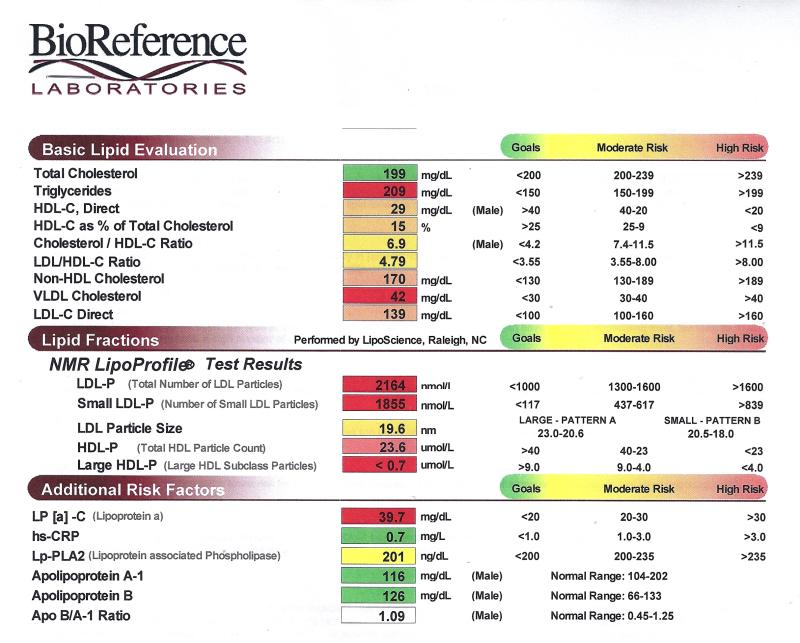
\includegraphics[width=0.7\textwidth]{img/variables_aleatorias_continuas/analitica_sanguinea.jpg}}
	\mode<presentation>{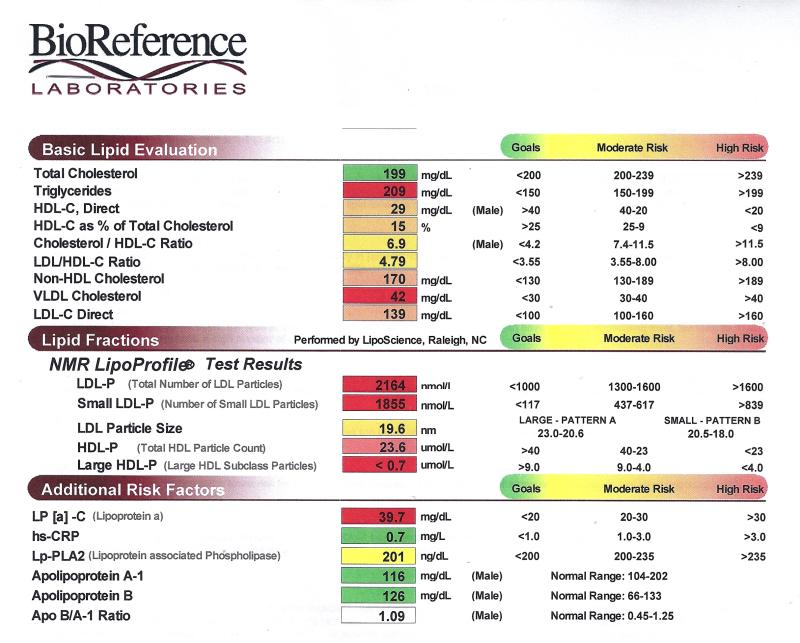
\includegraphics[width=\textwidth]{img/variables_aleatorias_continuas/analitica_sanguinea.jpg}}
\end{center}
\end{column}
\end{columns}
\end{frame}
	

%---------------------------------------------------------------------slide----
\begin{frame}
\frametitle{El teorema central del límite}
El comportamiento anterior lo presentan muchas variables continuas físicas y biológicas.

Si se piensa por ejemplo en la distribución de las estaturas, se verá que la mayor parte de los individuos presentan estaturas en torno a la
media, tanto por arriba, como por debajo, pero que a medida que van alejándose de la media, cada vez hay menos individuos con dichas
estaturas.

La justificación de que la distribución normal aparezca de manera tan frecuente en la naturaleza la encontramos en el
\highlight{\textbf{teorema central del límite}}, que veremos más adelante, y que establece que si una variable aleatoria continua proviene de un
experimento aleatorio cuyos resultados son debidos a un conjunto muy grande de factores independientes que actúan sumando sus efectos, entonces sigue una distribución aproximadamente normal.

\note{
Se ha observado que la mayor parte de las variables continuas físicas y biológicas presentan una distribucón con forma de campana de Gauss.

Si se piensa por ejemplo en la distribución de las estaturas, se verá que la mayor parte de los individuos presentan estaturas en torno a la
media, tanto por arriba, como por debajo, pero que a medida que van alejándose de la media, cada vez hay menos individuos con dichas
estaturas.

La justificación de que la distribución normal aparezca de manera tan frecuente en la naturaleza la encontramos en el
\structure{\textbf{teorema central del límite}}, que veremos más detenidamente en el siguiente tema, y que establece que si una variable
aleatoria $X$ proviene de un experimento aleatorio cuyos resultados son debidos a un conjunto muy grande de causas independientes que actúan
sumando sus efectos, entonces $X$ sigue una distribución aproximadamente normal.

Si pensamos en cualquier variable biológica, como por ejemplo la tensión arterial, rápidamente podremos identificar multitud de factores que
influyen en ella, como por ejemplo la edad, el sexo, la dieta, el ejercicio físico, si se fuma o no, etc. El valor de la tensión arterial en
un individuo es el resultado de todos estos factores que suman sus efectos de manera independiente, y por ello, el el colesterol acaba
teniendo una distribución normal.
}
\end{frame}


%---------------------------------------------------------------------slide----
\begin{frame}
\frametitle{La distribución Normal estándar $N(0,1)$}
De todas las distribuciones normales, la más importante es la que tiene media $\mu=0$ y desviación típica $\sigma=1$, que se conoce como \highlight{\textbf{normal estándar}} y se designa por $Z\sim N(0,1)$.

\begin{center}
	\tikzsetnextfilename{variables_aleatorias_continuas/funcion_densidad_normal_estandar}
	\mode<article>{\resizebox{0.6\textwidth}{!}{%% Input file name: funcion_densidad_normal_estandar.fig
%% FIG version: 3.2
%% Orientation: Landscape
%% Justification: Flush Left
%% Units: Inches
%% Paper size: A4
%% Magnification: 100.0
%% Resolution: 1200ppi
%% Include the following in the preamble:
%% \usepackage{textcomp}
%% End

\begin{pspicture}(6.69cm,3.44cm)(16.66cm,13.45cm)
\psset{unit=0.8cm}
%%
%% Depth: 2147483647
%%
\newgray{mycolor0}{0.74}\definecolor{mycolor0}{gray}{0.74}
\newrgbcolor{mycolor1}{1.00 0.50 0.31}\definecolor{mycolor1}{rgb}{1.00,0.50,0.31}
%%
%% Depth: 100
%%
\psset{linestyle=solid,linewidth=0.03175,linecolor=mycolor1,fillstyle=none}
\psline(10.61,6.75)(10.70,6.76)(10.80,6.77)(10.89,6.79)(10.99,6.80)(11.08,6.82)(11.17,6.84)(11.27,6.87)(11.36,6.90)(11.46,6.94)(11.55,6.98)(11.64,7.03)(11.74,7.08)(11.83,7.15)(11.93,7.22)(12.02,7.31)(12.12,7.40)(12.21,7.51)(12.30,7.63)(12.40,7.77)(12.49,7.92)(12.59,8.08)(12.68,8.26)(12.78,8.45)(12.87,8.67)(12.96,8.89)(13.06,9.14)(13.15,9.40)(13.25,9.67)(13.34,9.95)(13.43,10.26)(13.53,10.56)(13.62,10.88)(13.72,11.21)(13.81,11.54)(13.91,11.87)(14.00,12.20)(14.09,12.52)(14.19,12.84)(14.28,13.14)(14.38,13.43)(14.47,13.70)(14.56,13.96)(14.66,14.18)(14.76,14.38)(14.85,14.55)(14.94,14.69)(15.04,14.80)(15.13,14.87)(15.23,14.91)(15.32,14.91)(15.41,14.87)(15.51,14.80)(15.60,14.69)(15.70,14.55)(15.79,14.38)(15.89,14.18)(15.98,13.96)(16.07,13.70)(16.17,13.43)(16.26,13.14)(16.36,12.84)(16.45,12.52)(16.54,12.20)(16.64,11.87)(16.73,11.54)(16.83,11.21)(16.92,10.88)(17.02,10.56)(17.11,10.26)(17.20,9.95)(17.30,9.67)(17.39,9.40)(17.49,9.14)(17.58,8.89)(17.68,8.67)(17.77,8.45)(17.86,8.26)(17.96,8.08)(18.05,7.92)(18.15,7.77)(18.24,7.63)(18.33,7.51)(18.43,7.40)(18.52,7.31)(18.62,7.22)(18.71,7.15)(18.81,7.08)(18.90,7.03)(18.99,6.98)(19.09,6.94)(19.18,6.90)(19.28,6.87)(19.37,6.84)(19.47,6.82)(19.56,6.80)(19.66,6.79)(19.75,6.77)(19.84,6.76)(19.94,6.75)
\psset{linecolor=black}
\psline(11.02,6.43)(19.52,6.43)
\psline(11.02,6.43)(11.02,6.22)
\psline(12.44,6.43)(12.44,6.22)
\psline(13.86,6.43)(13.86,6.22)
\psline(15.27,6.43)(15.27,6.22)
\psline(16.69,6.43)(16.69,6.22)
\psline(18.11,6.43)(18.11,6.22)
\psline(19.52,6.43)(19.52,6.22)
\rput(11.02,5.67){-3}
\rput(12.44,5.67){-2}
\rput(13.86,5.67){-1}
\rput(15.27,5.67){0}
\rput(16.69,5.67){1}
\rput(18.11,5.67){2}
\rput(19.52,5.67){3}
\psline(10.23,6.72)(10.23,14.94)
\psline(10.23,6.72)(10.02,6.72)
\psline(10.23,8.77)(10.02,8.77)
\psline(10.23,10.83)(10.02,10.83)
\psline(10.23,12.88)(10.02,12.88)
\psline(10.23,14.94)(10.02,14.94)
\rput{90}(9.73,6.72){0.0}
\rput{90}(9.73,8.77){0.1}
\rput{90}(9.73,10.83){0.2}
\rput{90}(9.73,12.88){0.3}
\rput{90}(9.73,14.94){0.4}
\psline(10.23,6.43)(20.31,6.43)(20.31,15.23)(10.23,15.23)(10.23,6.43)
\rput[l](11.14,15.99){Distribución normal estándar $N(\mu=0,\sigma=1)$}
\rput(15.27,4.82){$Z$}
\rput[l]{90}(8.88,8.46){Densidad de probabilidad $f(z)$}
\psset{linecolor=mycolor0}
\psline(10.23,6.72)(20.31,6.72)
\end{pspicture}
%% End
}}
	\mode<presentation>{\resizebox{0.55\textwidth}{!}{%% Input file name: funcion_densidad_normal_estandar.fig
%% FIG version: 3.2
%% Orientation: Landscape
%% Justification: Flush Left
%% Units: Inches
%% Paper size: A4
%% Magnification: 100.0
%% Resolution: 1200ppi
%% Include the following in the preamble:
%% \usepackage{textcomp}
%% End

\begin{pspicture}(6.69cm,3.44cm)(16.66cm,13.45cm)
\psset{unit=0.8cm}
%%
%% Depth: 2147483647
%%
\newgray{mycolor0}{0.74}\definecolor{mycolor0}{gray}{0.74}
\newrgbcolor{mycolor1}{1.00 0.50 0.31}\definecolor{mycolor1}{rgb}{1.00,0.50,0.31}
%%
%% Depth: 100
%%
\psset{linestyle=solid,linewidth=0.03175,linecolor=mycolor1,fillstyle=none}
\psline(10.61,6.75)(10.70,6.76)(10.80,6.77)(10.89,6.79)(10.99,6.80)(11.08,6.82)(11.17,6.84)(11.27,6.87)(11.36,6.90)(11.46,6.94)(11.55,6.98)(11.64,7.03)(11.74,7.08)(11.83,7.15)(11.93,7.22)(12.02,7.31)(12.12,7.40)(12.21,7.51)(12.30,7.63)(12.40,7.77)(12.49,7.92)(12.59,8.08)(12.68,8.26)(12.78,8.45)(12.87,8.67)(12.96,8.89)(13.06,9.14)(13.15,9.40)(13.25,9.67)(13.34,9.95)(13.43,10.26)(13.53,10.56)(13.62,10.88)(13.72,11.21)(13.81,11.54)(13.91,11.87)(14.00,12.20)(14.09,12.52)(14.19,12.84)(14.28,13.14)(14.38,13.43)(14.47,13.70)(14.56,13.96)(14.66,14.18)(14.76,14.38)(14.85,14.55)(14.94,14.69)(15.04,14.80)(15.13,14.87)(15.23,14.91)(15.32,14.91)(15.41,14.87)(15.51,14.80)(15.60,14.69)(15.70,14.55)(15.79,14.38)(15.89,14.18)(15.98,13.96)(16.07,13.70)(16.17,13.43)(16.26,13.14)(16.36,12.84)(16.45,12.52)(16.54,12.20)(16.64,11.87)(16.73,11.54)(16.83,11.21)(16.92,10.88)(17.02,10.56)(17.11,10.26)(17.20,9.95)(17.30,9.67)(17.39,9.40)(17.49,9.14)(17.58,8.89)(17.68,8.67)(17.77,8.45)(17.86,8.26)(17.96,8.08)(18.05,7.92)(18.15,7.77)(18.24,7.63)(18.33,7.51)(18.43,7.40)(18.52,7.31)(18.62,7.22)(18.71,7.15)(18.81,7.08)(18.90,7.03)(18.99,6.98)(19.09,6.94)(19.18,6.90)(19.28,6.87)(19.37,6.84)(19.47,6.82)(19.56,6.80)(19.66,6.79)(19.75,6.77)(19.84,6.76)(19.94,6.75)
\psset{linecolor=black}
\psline(11.02,6.43)(19.52,6.43)
\psline(11.02,6.43)(11.02,6.22)
\psline(12.44,6.43)(12.44,6.22)
\psline(13.86,6.43)(13.86,6.22)
\psline(15.27,6.43)(15.27,6.22)
\psline(16.69,6.43)(16.69,6.22)
\psline(18.11,6.43)(18.11,6.22)
\psline(19.52,6.43)(19.52,6.22)
\rput(11.02,5.67){-3}
\rput(12.44,5.67){-2}
\rput(13.86,5.67){-1}
\rput(15.27,5.67){0}
\rput(16.69,5.67){1}
\rput(18.11,5.67){2}
\rput(19.52,5.67){3}
\psline(10.23,6.72)(10.23,14.94)
\psline(10.23,6.72)(10.02,6.72)
\psline(10.23,8.77)(10.02,8.77)
\psline(10.23,10.83)(10.02,10.83)
\psline(10.23,12.88)(10.02,12.88)
\psline(10.23,14.94)(10.02,14.94)
\rput{90}(9.73,6.72){0.0}
\rput{90}(9.73,8.77){0.1}
\rput{90}(9.73,10.83){0.2}
\rput{90}(9.73,12.88){0.3}
\rput{90}(9.73,14.94){0.4}
\psline(10.23,6.43)(20.31,6.43)(20.31,15.23)(10.23,15.23)(10.23,6.43)
\rput[l](11.14,15.99){Distribución normal estándar $N(\mu=0,\sigma=1)$}
\rput(15.27,4.82){$Z$}
\rput[l]{90}(8.88,8.46){Densidad de probabilidad $f(z)$}
\psset{linecolor=mycolor0}
\psline(10.23,6.72)(20.31,6.72)
\end{pspicture}
%% End
}}
\end{center}

\note{
De todas las distribuciones normales, la más importante es la que tiene media $\mu=0$ y desviación típica $\sigma=1$,
que se conoce como \highlight{\textbf{normal estándar}} y se designa por $Z$.

Su función de densidad será una campana de Gauss centrada en el 0, en la que el 99\% de los individuos estarán entre -3 y 3. 
}
\end{frame}


%---------------------------------------------------------------------slide----
\begin{frame}
\frametitle{Cálculo de probabilidades con la Normal estándar}
\framesubtitle{Manejo de la tabla de la función de distribución}
Para evitar tener que calcular probabilidades integrando la función de densidad de la normal estándar es habitual utilizar su función de
distribución, que se da en forma de tabla como la siguiente.

\begin{columns}
\begin{column}{0.47\textwidth}
\begin{center}
	Por ejemplo, para calcular $P(Z\leq 0.52)$
	
	\mode<article>{\begin{tabular}[b]
{|r||r|r|r|r|}
\hline
\multicolumn{1}{|c||}{$\mathbf{z}$}& 
\multicolumn{1}{c|}{\textbf{0,00}}& 
\multicolumn{1}{c|}{\textbf{0,01}}& 
\multicolumn{1}{c|}{\alert{\textbf{0,02}}}& 
\multicolumn{1}{c|}{\textbf{\cdots}}\\
\hline\hline
\textbf{0,0}& 
0,5000& 
0,5040& 
0,5080& 
\cdots\\
\hline
\textbf{0,1}& 
0,5398& 
0,5438& 
0,5478& 
\cdots \\
\hline
\textbf{0,2}& 
0,5793& 
0,5832& 
0,5871& 
\cdots\\
\hline
\textbf{0,3}& 
0,6179& 
0,6217& 
0,6255& 
\cdots\\
\hline
\textbf{0,4}& 
0,6554& 
0,6591& 
0,6628& 
\cdots\\
\hline
\alert{\textbf{0,5}}& 
0,6915& 
0,6950& 
\cellcolor{coral}{\alert{\textbf{0,6985}}}& 
\cdots\\
\hline
\textbf{\vdots}& 
\vdots& 
\vdots& 
\vdots& 
\ddots\\
\hline
\end{tabular}}
	\mode<presentation>{\scalebox{0.9}{\begin{tabular}[b]
{|r||r|r|r|r|}
\hline
\multicolumn{1}{|c||}{$\mathbf{z}$}& 
\multicolumn{1}{c|}{\textbf{0,00}}& 
\multicolumn{1}{c|}{\textbf{0,01}}& 
\multicolumn{1}{c|}{\alert{\textbf{0,02}}}& 
\multicolumn{1}{c|}{\textbf{\cdots}}\\
\hline\hline
\textbf{0,0}& 
0,5000& 
0,5040& 
0,5080& 
\cdots\\
\hline
\textbf{0,1}& 
0,5398& 
0,5438& 
0,5478& 
\cdots \\
\hline
\textbf{0,2}& 
0,5793& 
0,5832& 
0,5871& 
\cdots\\
\hline
\textbf{0,3}& 
0,6179& 
0,6217& 
0,6255& 
\cdots\\
\hline
\textbf{0,4}& 
0,6554& 
0,6591& 
0,6628& 
\cdots\\
\hline
\alert{\textbf{0,5}}& 
0,6915& 
0,6950& 
\cellcolor{coral}{\alert{\textbf{0,6985}}}& 
\cdots\\
\hline
\textbf{\vdots}& 
\vdots& 
\vdots& 
\vdots& 
\ddots\\
\hline
\end{tabular}}}
	
	$0.52 \rightarrow $ fila $0.5$ + columna $0.02$
\end{center}
\end{column}
\begin{column}{0.53\textwidth}
\begin{center}
	\tikzsetnextfilename{variables_aleatorias_continuas/calculo_probabilidades_normal_cola_izquierda}
	\mode<article>{\resizebox{0.6\textwidth}{!}{% Created by tikzDevice version 0.10.1 on 2016-05-16 22:15:16
% !TEX encoding = UTF-8 Unicode
\begin{tikzpicture}[x=1pt,y=1pt]
\definecolor{fillColor}{RGB}{255,255,255}
\path[use as bounding box,fill=fillColor,fill opacity=0.00] (0,0) rectangle (289.08,289.08);
\begin{scope}
\path[clip] (  0.00,  0.00) rectangle (289.08,289.08);
\definecolor{drawColor}{RGB}{0,0,0}

\node[text=drawColor,anchor=base,inner sep=0pt, outer sep=0pt, scale=  1.20] at (159.54,266.89) {\bfseries Distribución Normal estándar $N(0,1)$};

\node[text=drawColor,anchor=base,inner sep=0pt, outer sep=0pt, scale=  1.00] at (159.54,  6.00) {X};

\node[text=drawColor,rotate= 90.00,anchor=base,inner sep=0pt, outer sep=0pt, scale=  1.00] at ( 13.20,147.54) {Densidad de probabilidad $f(x)$};
\end{scope}
\begin{scope}
\path[clip] (  0.00,  0.00) rectangle (289.08,289.08);
\definecolor{drawColor}{RGB}{0,0,0}

\path[draw=drawColor,line width= 0.4pt,line join=round,line cap=round] (176.59, 42.00) -- (176.59, 42.00);

\path[draw=drawColor,line width= 0.4pt,line join=round,line cap=round] (176.59, 42.00) -- (176.59, 36.00);

\node[text=drawColor,anchor=base,inner sep=0pt, outer sep=0pt, scale=  1.00] at (176.59, 25.20) {0.52};
\end{scope}
\begin{scope}
\path[clip] ( 42.00, 42.00) rectangle (277.08,253.08);
\definecolor{fillColor}{RGB}{238,50,36}

\path[fill=fillColor,fill opacity=0.39] ( 50.71, 42.00) --
	( 50.71, 42.76) --
	( 52.02, 42.86) --
	( 53.33, 42.98) --
	( 54.64, 43.12) --
	( 55.95, 43.27) --
	( 57.26, 43.44) --
	( 58.57, 43.63) --
	( 59.89, 43.84) --
	( 61.20, 44.08) --
	( 62.51, 44.34) --
	( 63.82, 44.63) --
	( 65.13, 44.96) --
	( 66.44, 45.32) --
	( 67.75, 45.71) --
	( 69.06, 46.15) --
	( 70.38, 46.63) --
	( 71.69, 47.16) --
	( 73.00, 47.74) --
	( 74.31, 48.37) --
	( 75.62, 49.06) --
	( 76.93, 49.82) --
	( 78.24, 50.64) --
	( 79.55, 51.54) --
	( 80.87, 52.50) --
	( 82.18, 53.55) --
	( 83.49, 54.69) --
	( 84.80, 55.91) --
	( 86.11, 57.23) --
	( 87.42, 58.64) --
	( 88.73, 60.16) --
	( 90.04, 61.78) --
	( 91.36, 63.51) --
	( 92.67, 65.36) --
	( 93.98, 67.33) --
	( 95.29, 69.41) --
	( 96.60, 71.62) --
	( 97.91, 73.96) --
	( 99.22, 76.43) --
	(100.53, 79.03) --
	(101.85, 81.77) --
	(103.16, 84.63) --
	(104.47, 87.63) --
	(105.78, 90.76) --
	(107.09, 94.03) --
	(108.40, 97.42) --
	(109.71,100.95) --
	(111.02,104.59) --
	(112.34,108.35) --
	(113.65,112.23) --
	(114.96,116.22) --
	(116.27,120.30) --
	(117.58,124.48) --
	(118.89,128.75) --
	(120.20,133.09) --
	(121.51,137.49) --
	(122.83,141.94) --
	(124.14,146.44) --
	(125.45,150.96) --
	(126.76,155.50) --
	(128.07,160.04) --
	(129.38,164.56) --
	(130.69,169.05) --
	(132.00,173.50) --
	(133.32,177.88) --
	(134.63,182.19) --
	(135.94,186.40) --
	(137.25,190.50) --
	(138.56,194.48) --
	(139.87,198.30) --
	(141.18,201.97) --
	(142.49,205.47) --
	(143.81,208.77) --
	(145.12,211.87) --
	(146.43,214.74) --
	(147.74,217.39) --
	(149.05,219.79) --
	(150.36,221.94) --
	(151.67,223.82) --
	(152.98,225.43) --
	(154.30,226.75) --
	(155.61,227.79) --
	(156.92,228.53) --
	(158.23,228.98) --
	(159.54,229.13) --
	(160.85,228.98) --
	(162.16,228.53) --
	(163.47,227.79) --
	(164.78,226.75) --
	(166.10,225.43) --
	(167.41,223.82) --
	(168.72,221.94) --
	(170.03,219.79) --
	(171.34,217.39) --
	(172.65,214.74) --
	(173.96,211.87) --
	(175.27,208.77) --
	(176.59,205.47) --
	(176.59, 42.00) --
	cycle;
\definecolor{drawColor}{RGB}{5,161,230}

\path[draw=drawColor,line width= 0.8pt,line join=round,line cap=round] ( 50.71, 42.76) --
	( 52.02, 42.86) --
	( 53.33, 42.98) --
	( 54.64, 43.12) --
	( 55.95, 43.27) --
	( 57.26, 43.44) --
	( 58.57, 43.63) --
	( 59.89, 43.84) --
	( 61.20, 44.08) --
	( 62.51, 44.34) --
	( 63.82, 44.63) --
	( 65.13, 44.96) --
	( 66.44, 45.32) --
	( 67.75, 45.71) --
	( 69.06, 46.15) --
	( 70.38, 46.63) --
	( 71.69, 47.16) --
	( 73.00, 47.74) --
	( 74.31, 48.37) --
	( 75.62, 49.06) --
	( 76.93, 49.82) --
	( 78.24, 50.64) --
	( 79.55, 51.54) --
	( 80.87, 52.50) --
	( 82.18, 53.55) --
	( 83.49, 54.69) --
	( 84.80, 55.91) --
	( 86.11, 57.23) --
	( 87.42, 58.64) --
	( 88.73, 60.16) --
	( 90.04, 61.78) --
	( 91.36, 63.51) --
	( 92.67, 65.36) --
	( 93.98, 67.33) --
	( 95.29, 69.41) --
	( 96.60, 71.62) --
	( 97.91, 73.96) --
	( 99.22, 76.43) --
	(100.53, 79.03) --
	(101.85, 81.77) --
	(103.16, 84.63) --
	(104.47, 87.63) --
	(105.78, 90.76) --
	(107.09, 94.03) --
	(108.40, 97.42) --
	(109.71,100.95) --
	(111.02,104.59) --
	(112.34,108.35) --
	(113.65,112.23) --
	(114.96,116.22) --
	(116.27,120.30) --
	(117.58,124.48) --
	(118.89,128.75) --
	(120.20,133.09) --
	(121.51,137.49) --
	(122.83,141.94) --
	(124.14,146.44) --
	(125.45,150.96) --
	(126.76,155.50) --
	(128.07,160.04) --
	(129.38,164.56) --
	(130.69,169.05) --
	(132.00,173.50) --
	(133.32,177.88) --
	(134.63,182.19) --
	(135.94,186.40) --
	(137.25,190.50) --
	(138.56,194.48) --
	(139.87,198.30) --
	(141.18,201.97) --
	(142.49,205.47) --
	(143.81,208.77) --
	(145.12,211.87) --
	(146.43,214.74) --
	(147.74,217.39) --
	(149.05,219.79) --
	(150.36,221.94) --
	(151.67,223.82) --
	(152.98,225.43) --
	(154.30,226.75) --
	(155.61,227.79) --
	(156.92,228.53) --
	(158.23,228.98) --
	(159.54,229.13) --
	(160.85,228.98) --
	(162.16,228.53) --
	(163.47,227.79) --
	(164.78,226.75) --
	(166.10,225.43) --
	(167.41,223.82) --
	(168.72,221.94) --
	(170.03,219.79) --
	(171.34,217.39) --
	(172.65,214.74) --
	(173.96,211.87) --
	(175.27,208.77) --
	(176.59,205.47) --
	(177.90,201.97) --
	(179.21,198.30) --
	(180.52,194.48) --
	(181.83,190.50) --
	(183.14,186.40) --
	(184.45,182.19) --
	(185.76,177.88) --
	(187.08,173.50) --
	(188.39,169.05) --
	(189.70,164.56) --
	(191.01,160.04) --
	(192.32,155.50) --
	(193.63,150.96) --
	(194.94,146.44) --
	(196.25,141.94) --
	(197.57,137.49) --
	(198.88,133.09) --
	(200.19,128.75) --
	(201.50,124.48) --
	(202.81,120.30) --
	(204.12,116.22) --
	(205.43,112.23) --
	(206.74,108.35) --
	(208.06,104.59) --
	(209.37,100.95) --
	(210.68, 97.42) --
	(211.99, 94.03) --
	(213.30, 90.76) --
	(214.61, 87.63) --
	(215.92, 84.63) --
	(217.23, 81.77) --
	(218.55, 79.03) --
	(219.86, 76.43) --
	(221.17, 73.96) --
	(222.48, 71.62) --
	(223.79, 69.41) --
	(225.10, 67.33) --
	(226.41, 65.36) --
	(227.72, 63.51) --
	(229.04, 61.78) --
	(230.35, 60.16) --
	(231.66, 58.64) --
	(232.97, 57.23) --
	(234.28, 55.91) --
	(235.59, 54.69) --
	(236.90, 53.55) --
	(238.21, 52.50) --
	(239.53, 51.54) --
	(240.84, 50.64) --
	(242.15, 49.82) --
	(243.46, 49.06) --
	(244.77, 48.37) --
	(246.08, 47.74) --
	(247.39, 47.16) --
	(248.70, 46.63) --
	(250.02, 46.15) --
	(251.33, 45.71) --
	(252.64, 45.32) --
	(253.95, 44.96) --
	(255.26, 44.63) --
	(256.57, 44.34) --
	(257.88, 44.08) --
	(259.19, 43.84) --
	(260.51, 43.63) --
	(261.82, 43.44) --
	(263.13, 43.27) --
	(264.44, 43.12) --
	(265.75, 42.98) --
	(267.06, 42.86) --
	(268.37, 42.76);
\definecolor{drawColor}{RGB}{0,0,0}

\node[text=drawColor,anchor=base,inner sep=0pt, outer sep=0pt, scale=  1.00] at (136.59, 67.64) {F( 0.52 )= 0.6985};
\end{scope}
\begin{scope}
\path[clip] (  0.00,  0.00) rectangle (289.08,289.08);
\definecolor{drawColor}{RGB}{0,0,0}

\path[draw=drawColor,line width= 0.4pt,line join=round,line cap=round] ( 42.00, 42.00) --
	(277.08, 42.00) --
	(277.08,253.08) --
	( 42.00,253.08) --
	( 42.00, 42.00);
\end{scope}
\end{tikzpicture}
}}
	\mode<presentation>{\resizebox{0.9\textwidth}{!}{% Created by tikzDevice version 0.10.1 on 2016-05-16 22:15:16
% !TEX encoding = UTF-8 Unicode
\begin{tikzpicture}[x=1pt,y=1pt]
\definecolor{fillColor}{RGB}{255,255,255}
\path[use as bounding box,fill=fillColor,fill opacity=0.00] (0,0) rectangle (289.08,289.08);
\begin{scope}
\path[clip] (  0.00,  0.00) rectangle (289.08,289.08);
\definecolor{drawColor}{RGB}{0,0,0}

\node[text=drawColor,anchor=base,inner sep=0pt, outer sep=0pt, scale=  1.20] at (159.54,266.89) {\bfseries Distribución Normal estándar $N(0,1)$};

\node[text=drawColor,anchor=base,inner sep=0pt, outer sep=0pt, scale=  1.00] at (159.54,  6.00) {X};

\node[text=drawColor,rotate= 90.00,anchor=base,inner sep=0pt, outer sep=0pt, scale=  1.00] at ( 13.20,147.54) {Densidad de probabilidad $f(x)$};
\end{scope}
\begin{scope}
\path[clip] (  0.00,  0.00) rectangle (289.08,289.08);
\definecolor{drawColor}{RGB}{0,0,0}

\path[draw=drawColor,line width= 0.4pt,line join=round,line cap=round] (176.59, 42.00) -- (176.59, 42.00);

\path[draw=drawColor,line width= 0.4pt,line join=round,line cap=round] (176.59, 42.00) -- (176.59, 36.00);

\node[text=drawColor,anchor=base,inner sep=0pt, outer sep=0pt, scale=  1.00] at (176.59, 25.20) {0.52};
\end{scope}
\begin{scope}
\path[clip] ( 42.00, 42.00) rectangle (277.08,253.08);
\definecolor{fillColor}{RGB}{238,50,36}

\path[fill=fillColor,fill opacity=0.39] ( 50.71, 42.00) --
	( 50.71, 42.76) --
	( 52.02, 42.86) --
	( 53.33, 42.98) --
	( 54.64, 43.12) --
	( 55.95, 43.27) --
	( 57.26, 43.44) --
	( 58.57, 43.63) --
	( 59.89, 43.84) --
	( 61.20, 44.08) --
	( 62.51, 44.34) --
	( 63.82, 44.63) --
	( 65.13, 44.96) --
	( 66.44, 45.32) --
	( 67.75, 45.71) --
	( 69.06, 46.15) --
	( 70.38, 46.63) --
	( 71.69, 47.16) --
	( 73.00, 47.74) --
	( 74.31, 48.37) --
	( 75.62, 49.06) --
	( 76.93, 49.82) --
	( 78.24, 50.64) --
	( 79.55, 51.54) --
	( 80.87, 52.50) --
	( 82.18, 53.55) --
	( 83.49, 54.69) --
	( 84.80, 55.91) --
	( 86.11, 57.23) --
	( 87.42, 58.64) --
	( 88.73, 60.16) --
	( 90.04, 61.78) --
	( 91.36, 63.51) --
	( 92.67, 65.36) --
	( 93.98, 67.33) --
	( 95.29, 69.41) --
	( 96.60, 71.62) --
	( 97.91, 73.96) --
	( 99.22, 76.43) --
	(100.53, 79.03) --
	(101.85, 81.77) --
	(103.16, 84.63) --
	(104.47, 87.63) --
	(105.78, 90.76) --
	(107.09, 94.03) --
	(108.40, 97.42) --
	(109.71,100.95) --
	(111.02,104.59) --
	(112.34,108.35) --
	(113.65,112.23) --
	(114.96,116.22) --
	(116.27,120.30) --
	(117.58,124.48) --
	(118.89,128.75) --
	(120.20,133.09) --
	(121.51,137.49) --
	(122.83,141.94) --
	(124.14,146.44) --
	(125.45,150.96) --
	(126.76,155.50) --
	(128.07,160.04) --
	(129.38,164.56) --
	(130.69,169.05) --
	(132.00,173.50) --
	(133.32,177.88) --
	(134.63,182.19) --
	(135.94,186.40) --
	(137.25,190.50) --
	(138.56,194.48) --
	(139.87,198.30) --
	(141.18,201.97) --
	(142.49,205.47) --
	(143.81,208.77) --
	(145.12,211.87) --
	(146.43,214.74) --
	(147.74,217.39) --
	(149.05,219.79) --
	(150.36,221.94) --
	(151.67,223.82) --
	(152.98,225.43) --
	(154.30,226.75) --
	(155.61,227.79) --
	(156.92,228.53) --
	(158.23,228.98) --
	(159.54,229.13) --
	(160.85,228.98) --
	(162.16,228.53) --
	(163.47,227.79) --
	(164.78,226.75) --
	(166.10,225.43) --
	(167.41,223.82) --
	(168.72,221.94) --
	(170.03,219.79) --
	(171.34,217.39) --
	(172.65,214.74) --
	(173.96,211.87) --
	(175.27,208.77) --
	(176.59,205.47) --
	(176.59, 42.00) --
	cycle;
\definecolor{drawColor}{RGB}{5,161,230}

\path[draw=drawColor,line width= 0.8pt,line join=round,line cap=round] ( 50.71, 42.76) --
	( 52.02, 42.86) --
	( 53.33, 42.98) --
	( 54.64, 43.12) --
	( 55.95, 43.27) --
	( 57.26, 43.44) --
	( 58.57, 43.63) --
	( 59.89, 43.84) --
	( 61.20, 44.08) --
	( 62.51, 44.34) --
	( 63.82, 44.63) --
	( 65.13, 44.96) --
	( 66.44, 45.32) --
	( 67.75, 45.71) --
	( 69.06, 46.15) --
	( 70.38, 46.63) --
	( 71.69, 47.16) --
	( 73.00, 47.74) --
	( 74.31, 48.37) --
	( 75.62, 49.06) --
	( 76.93, 49.82) --
	( 78.24, 50.64) --
	( 79.55, 51.54) --
	( 80.87, 52.50) --
	( 82.18, 53.55) --
	( 83.49, 54.69) --
	( 84.80, 55.91) --
	( 86.11, 57.23) --
	( 87.42, 58.64) --
	( 88.73, 60.16) --
	( 90.04, 61.78) --
	( 91.36, 63.51) --
	( 92.67, 65.36) --
	( 93.98, 67.33) --
	( 95.29, 69.41) --
	( 96.60, 71.62) --
	( 97.91, 73.96) --
	( 99.22, 76.43) --
	(100.53, 79.03) --
	(101.85, 81.77) --
	(103.16, 84.63) --
	(104.47, 87.63) --
	(105.78, 90.76) --
	(107.09, 94.03) --
	(108.40, 97.42) --
	(109.71,100.95) --
	(111.02,104.59) --
	(112.34,108.35) --
	(113.65,112.23) --
	(114.96,116.22) --
	(116.27,120.30) --
	(117.58,124.48) --
	(118.89,128.75) --
	(120.20,133.09) --
	(121.51,137.49) --
	(122.83,141.94) --
	(124.14,146.44) --
	(125.45,150.96) --
	(126.76,155.50) --
	(128.07,160.04) --
	(129.38,164.56) --
	(130.69,169.05) --
	(132.00,173.50) --
	(133.32,177.88) --
	(134.63,182.19) --
	(135.94,186.40) --
	(137.25,190.50) --
	(138.56,194.48) --
	(139.87,198.30) --
	(141.18,201.97) --
	(142.49,205.47) --
	(143.81,208.77) --
	(145.12,211.87) --
	(146.43,214.74) --
	(147.74,217.39) --
	(149.05,219.79) --
	(150.36,221.94) --
	(151.67,223.82) --
	(152.98,225.43) --
	(154.30,226.75) --
	(155.61,227.79) --
	(156.92,228.53) --
	(158.23,228.98) --
	(159.54,229.13) --
	(160.85,228.98) --
	(162.16,228.53) --
	(163.47,227.79) --
	(164.78,226.75) --
	(166.10,225.43) --
	(167.41,223.82) --
	(168.72,221.94) --
	(170.03,219.79) --
	(171.34,217.39) --
	(172.65,214.74) --
	(173.96,211.87) --
	(175.27,208.77) --
	(176.59,205.47) --
	(177.90,201.97) --
	(179.21,198.30) --
	(180.52,194.48) --
	(181.83,190.50) --
	(183.14,186.40) --
	(184.45,182.19) --
	(185.76,177.88) --
	(187.08,173.50) --
	(188.39,169.05) --
	(189.70,164.56) --
	(191.01,160.04) --
	(192.32,155.50) --
	(193.63,150.96) --
	(194.94,146.44) --
	(196.25,141.94) --
	(197.57,137.49) --
	(198.88,133.09) --
	(200.19,128.75) --
	(201.50,124.48) --
	(202.81,120.30) --
	(204.12,116.22) --
	(205.43,112.23) --
	(206.74,108.35) --
	(208.06,104.59) --
	(209.37,100.95) --
	(210.68, 97.42) --
	(211.99, 94.03) --
	(213.30, 90.76) --
	(214.61, 87.63) --
	(215.92, 84.63) --
	(217.23, 81.77) --
	(218.55, 79.03) --
	(219.86, 76.43) --
	(221.17, 73.96) --
	(222.48, 71.62) --
	(223.79, 69.41) --
	(225.10, 67.33) --
	(226.41, 65.36) --
	(227.72, 63.51) --
	(229.04, 61.78) --
	(230.35, 60.16) --
	(231.66, 58.64) --
	(232.97, 57.23) --
	(234.28, 55.91) --
	(235.59, 54.69) --
	(236.90, 53.55) --
	(238.21, 52.50) --
	(239.53, 51.54) --
	(240.84, 50.64) --
	(242.15, 49.82) --
	(243.46, 49.06) --
	(244.77, 48.37) --
	(246.08, 47.74) --
	(247.39, 47.16) --
	(248.70, 46.63) --
	(250.02, 46.15) --
	(251.33, 45.71) --
	(252.64, 45.32) --
	(253.95, 44.96) --
	(255.26, 44.63) --
	(256.57, 44.34) --
	(257.88, 44.08) --
	(259.19, 43.84) --
	(260.51, 43.63) --
	(261.82, 43.44) --
	(263.13, 43.27) --
	(264.44, 43.12) --
	(265.75, 42.98) --
	(267.06, 42.86) --
	(268.37, 42.76);
\definecolor{drawColor}{RGB}{0,0,0}

\node[text=drawColor,anchor=base,inner sep=0pt, outer sep=0pt, scale=  1.00] at (136.59, 67.64) {F( 0.52 )= 0.6985};
\end{scope}
\begin{scope}
\path[clip] (  0.00,  0.00) rectangle (289.08,289.08);
\definecolor{drawColor}{RGB}{0,0,0}

\path[draw=drawColor,line width= 0.4pt,line join=round,line cap=round] ( 42.00, 42.00) --
	(277.08, 42.00) --
	(277.08,253.08) --
	( 42.00,253.08) --
	( 42.00, 42.00);
\end{scope}
\end{tikzpicture}
}}
\end{center}
\end{column}
\end{columns}

\note{
Para evitar tener que calcular probabilidades integrando la función de densidad de la normal estándar se suele utilizar su función de
distribución.

Habitualmente se suele manejar una tabla con los valores de la función de distribución tabulados cada centésima. En esta tabla, la primera
columna contiene las décimas y la primera fila las centésimas, de forma que si por ejemplo queremos medir la probabilidad acumulada hasta el
$0.52$, tenemos que ir hasta la casilla correspondiente a la fila $0.5$  (5 décimas) y hasta la columna $0.02$ (2 centésimas), donde aparece
la probabilidad acumulada $0.6985$ y esta sería el área que queda por debajo de la campana de Gauss de la normal estándar entre $-\infty$ y
$0.52$.
}
\end{frame}


%---------------------------------------------------------------------slide----
\begin{frame}
\frametitle{Cálculo de probabilidades con la Normal estándar}
\framesubtitle{Probabilidades acumuladas por encima de un valor}
Cuando tengamos que calcular probabilidades acumuladas por encima de un determinado valor (cola de acumulación a la derecha), podemos hacerlo por medio de la probabilidad del suceso contrario.
Por ejemplo, 
\[
P(Z>0.52) =1-P(Z\leq 0.52) = 1-F(0.52) = 1 - 0.6985 = 0.3015.
\]
\begin{center}
	\tikzsetnextfilename{variables_aleatorias_continuas/calculo_probabilidades_normal_cola_derecha}
	\mode<article>{\resizebox{0.6\textwidth}{!}{% Created by tikzDevice version 0.10.1 on 2016-05-16 22:15:26
% !TEX encoding = UTF-8 Unicode
\begin{tikzpicture}[x=1pt,y=1pt]
\definecolor{fillColor}{RGB}{255,255,255}
\path[use as bounding box,fill=fillColor,fill opacity=0.00] (0,0) rectangle (289.08,289.08);
\begin{scope}
\path[clip] (  0.00,  0.00) rectangle (289.08,289.08);
\definecolor{drawColor}{RGB}{0,0,0}

\node[text=drawColor,anchor=base,inner sep=0pt, outer sep=0pt, scale=  1.20] at (159.54,266.89) {\bfseries Distribución Normal estándar $N(0,1)$};

\node[text=drawColor,anchor=base,inner sep=0pt, outer sep=0pt, scale=  1.00] at (159.54,  6.00) {X};

\node[text=drawColor,rotate= 90.00,anchor=base,inner sep=0pt, outer sep=0pt, scale=  1.00] at ( 13.20,147.54) {Densidad de probabilidad $f(x)$};
\end{scope}
\begin{scope}
\path[clip] (  0.00,  0.00) rectangle (289.08,289.08);
\definecolor{drawColor}{RGB}{0,0,0}

\path[draw=drawColor,line width= 0.4pt,line join=round,line cap=round] (176.59, 42.00) -- (176.59, 42.00);

\path[draw=drawColor,line width= 0.4pt,line join=round,line cap=round] (176.59, 42.00) -- (176.59, 36.00);

\node[text=drawColor,anchor=base,inner sep=0pt, outer sep=0pt, scale=  1.00] at (176.59, 25.20) {0.52};
\end{scope}
\begin{scope}
\path[clip] ( 42.00, 42.00) rectangle (277.08,253.08);
\definecolor{fillColor}{RGB}{238,50,36}

\path[fill=fillColor,fill opacity=0.39] (176.59, 42.00) --
	(176.59,205.47) --
	(177.90,201.97) --
	(179.21,198.30) --
	(180.52,194.48) --
	(181.83,190.50) --
	(183.14,186.40) --
	(184.45,182.19) --
	(185.76,177.88) --
	(187.08,173.50) --
	(188.39,169.05) --
	(189.70,164.56) --
	(191.01,160.04) --
	(192.32,155.50) --
	(193.63,150.96) --
	(194.94,146.44) --
	(196.25,141.94) --
	(197.57,137.49) --
	(198.88,133.09) --
	(200.19,128.75) --
	(201.50,124.48) --
	(202.81,120.30) --
	(204.12,116.22) --
	(205.43,112.23) --
	(206.74,108.35) --
	(208.06,104.59) --
	(209.37,100.95) --
	(210.68, 97.42) --
	(211.99, 94.03) --
	(213.30, 90.76) --
	(214.61, 87.63) --
	(215.92, 84.63) --
	(217.23, 81.77) --
	(218.55, 79.03) --
	(219.86, 76.43) --
	(221.17, 73.96) --
	(222.48, 71.62) --
	(223.79, 69.41) --
	(225.10, 67.33) --
	(226.41, 65.36) --
	(227.72, 63.51) --
	(229.04, 61.78) --
	(230.35, 60.16) --
	(231.66, 58.64) --
	(232.97, 57.23) --
	(234.28, 55.91) --
	(235.59, 54.69) --
	(236.90, 53.55) --
	(238.21, 52.50) --
	(239.53, 51.54) --
	(240.84, 50.64) --
	(242.15, 49.82) --
	(243.46, 49.06) --
	(244.77, 48.37) --
	(246.08, 47.74) --
	(247.39, 47.16) --
	(248.70, 46.63) --
	(250.02, 46.15) --
	(251.33, 45.71) --
	(252.64, 45.32) --
	(253.95, 44.96) --
	(255.26, 44.63) --
	(256.57, 44.34) --
	(257.88, 44.08) --
	(259.19, 43.84) --
	(260.51, 43.63) --
	(261.82, 43.44) --
	(263.13, 43.27) --
	(264.44, 43.12) --
	(265.75, 42.98) --
	(267.06, 42.86) --
	(268.37, 42.76) --
	(268.37, 42.00) --
	cycle;
\definecolor{drawColor}{RGB}{5,161,230}

\path[draw=drawColor,line width= 0.8pt,line join=round,line cap=round] ( 50.71, 42.76) --
	( 52.02, 42.86) --
	( 53.33, 42.98) --
	( 54.64, 43.12) --
	( 55.95, 43.27) --
	( 57.26, 43.44) --
	( 58.57, 43.63) --
	( 59.89, 43.84) --
	( 61.20, 44.08) --
	( 62.51, 44.34) --
	( 63.82, 44.63) --
	( 65.13, 44.96) --
	( 66.44, 45.32) --
	( 67.75, 45.71) --
	( 69.06, 46.15) --
	( 70.38, 46.63) --
	( 71.69, 47.16) --
	( 73.00, 47.74) --
	( 74.31, 48.37) --
	( 75.62, 49.06) --
	( 76.93, 49.82) --
	( 78.24, 50.64) --
	( 79.55, 51.54) --
	( 80.87, 52.50) --
	( 82.18, 53.55) --
	( 83.49, 54.69) --
	( 84.80, 55.91) --
	( 86.11, 57.23) --
	( 87.42, 58.64) --
	( 88.73, 60.16) --
	( 90.04, 61.78) --
	( 91.36, 63.51) --
	( 92.67, 65.36) --
	( 93.98, 67.33) --
	( 95.29, 69.41) --
	( 96.60, 71.62) --
	( 97.91, 73.96) --
	( 99.22, 76.43) --
	(100.53, 79.03) --
	(101.85, 81.77) --
	(103.16, 84.63) --
	(104.47, 87.63) --
	(105.78, 90.76) --
	(107.09, 94.03) --
	(108.40, 97.42) --
	(109.71,100.95) --
	(111.02,104.59) --
	(112.34,108.35) --
	(113.65,112.23) --
	(114.96,116.22) --
	(116.27,120.30) --
	(117.58,124.48) --
	(118.89,128.75) --
	(120.20,133.09) --
	(121.51,137.49) --
	(122.83,141.94) --
	(124.14,146.44) --
	(125.45,150.96) --
	(126.76,155.50) --
	(128.07,160.04) --
	(129.38,164.56) --
	(130.69,169.05) --
	(132.00,173.50) --
	(133.32,177.88) --
	(134.63,182.19) --
	(135.94,186.40) --
	(137.25,190.50) --
	(138.56,194.48) --
	(139.87,198.30) --
	(141.18,201.97) --
	(142.49,205.47) --
	(143.81,208.77) --
	(145.12,211.87) --
	(146.43,214.74) --
	(147.74,217.39) --
	(149.05,219.79) --
	(150.36,221.94) --
	(151.67,223.82) --
	(152.98,225.43) --
	(154.30,226.75) --
	(155.61,227.79) --
	(156.92,228.53) --
	(158.23,228.98) --
	(159.54,229.13) --
	(160.85,228.98) --
	(162.16,228.53) --
	(163.47,227.79) --
	(164.78,226.75) --
	(166.10,225.43) --
	(167.41,223.82) --
	(168.72,221.94) --
	(170.03,219.79) --
	(171.34,217.39) --
	(172.65,214.74) --
	(173.96,211.87) --
	(175.27,208.77) --
	(176.59,205.47) --
	(177.90,201.97) --
	(179.21,198.30) --
	(180.52,194.48) --
	(181.83,190.50) --
	(183.14,186.40) --
	(184.45,182.19) --
	(185.76,177.88) --
	(187.08,173.50) --
	(188.39,169.05) --
	(189.70,164.56) --
	(191.01,160.04) --
	(192.32,155.50) --
	(193.63,150.96) --
	(194.94,146.44) --
	(196.25,141.94) --
	(197.57,137.49) --
	(198.88,133.09) --
	(200.19,128.75) --
	(201.50,124.48) --
	(202.81,120.30) --
	(204.12,116.22) --
	(205.43,112.23) --
	(206.74,108.35) --
	(208.06,104.59) --
	(209.37,100.95) --
	(210.68, 97.42) --
	(211.99, 94.03) --
	(213.30, 90.76) --
	(214.61, 87.63) --
	(215.92, 84.63) --
	(217.23, 81.77) --
	(218.55, 79.03) --
	(219.86, 76.43) --
	(221.17, 73.96) --
	(222.48, 71.62) --
	(223.79, 69.41) --
	(225.10, 67.33) --
	(226.41, 65.36) --
	(227.72, 63.51) --
	(229.04, 61.78) --
	(230.35, 60.16) --
	(231.66, 58.64) --
	(232.97, 57.23) --
	(234.28, 55.91) --
	(235.59, 54.69) --
	(236.90, 53.55) --
	(238.21, 52.50) --
	(239.53, 51.54) --
	(240.84, 50.64) --
	(242.15, 49.82) --
	(243.46, 49.06) --
	(244.77, 48.37) --
	(246.08, 47.74) --
	(247.39, 47.16) --
	(248.70, 46.63) --
	(250.02, 46.15) --
	(251.33, 45.71) --
	(252.64, 45.32) --
	(253.95, 44.96) --
	(255.26, 44.63) --
	(256.57, 44.34) --
	(257.88, 44.08) --
	(259.19, 43.84) --
	(260.51, 43.63) --
	(261.82, 43.44) --
	(263.13, 43.27) --
	(264.44, 43.12) --
	(265.75, 42.98) --
	(267.06, 42.86) --
	(268.37, 42.76);
\definecolor{drawColor}{RGB}{0,0,0}

\node[text=drawColor,anchor=base,inner sep=0pt, outer sep=0pt, scale=  1.00] at (136.59, 67.64) {F( 0.52 )= 0.6985};

\node[text=drawColor,anchor=base,inner sep=0pt, outer sep=0pt, scale=  1.00] at (198.88, 67.64) {1-F( 0.52 )};

\node[text=drawColor,anchor=base,inner sep=0pt, outer sep=0pt, scale=  1.00] at (198.88, 57.61) {=0.3015};
\end{scope}
\begin{scope}
\path[clip] (  0.00,  0.00) rectangle (289.08,289.08);
\definecolor{drawColor}{RGB}{0,0,0}

\path[draw=drawColor,line width= 0.4pt,line join=round,line cap=round] ( 42.00, 42.00) --
	(277.08, 42.00) --
	(277.08,253.08) --
	( 42.00,253.08) --
	( 42.00, 42.00);
\end{scope}
\end{tikzpicture}
}}
	\mode<presentation>{\resizebox{0.5\textwidth}{!}{% Created by tikzDevice version 0.10.1 on 2016-05-16 22:15:26
% !TEX encoding = UTF-8 Unicode
\begin{tikzpicture}[x=1pt,y=1pt]
\definecolor{fillColor}{RGB}{255,255,255}
\path[use as bounding box,fill=fillColor,fill opacity=0.00] (0,0) rectangle (289.08,289.08);
\begin{scope}
\path[clip] (  0.00,  0.00) rectangle (289.08,289.08);
\definecolor{drawColor}{RGB}{0,0,0}

\node[text=drawColor,anchor=base,inner sep=0pt, outer sep=0pt, scale=  1.20] at (159.54,266.89) {\bfseries Distribución Normal estándar $N(0,1)$};

\node[text=drawColor,anchor=base,inner sep=0pt, outer sep=0pt, scale=  1.00] at (159.54,  6.00) {X};

\node[text=drawColor,rotate= 90.00,anchor=base,inner sep=0pt, outer sep=0pt, scale=  1.00] at ( 13.20,147.54) {Densidad de probabilidad $f(x)$};
\end{scope}
\begin{scope}
\path[clip] (  0.00,  0.00) rectangle (289.08,289.08);
\definecolor{drawColor}{RGB}{0,0,0}

\path[draw=drawColor,line width= 0.4pt,line join=round,line cap=round] (176.59, 42.00) -- (176.59, 42.00);

\path[draw=drawColor,line width= 0.4pt,line join=round,line cap=round] (176.59, 42.00) -- (176.59, 36.00);

\node[text=drawColor,anchor=base,inner sep=0pt, outer sep=0pt, scale=  1.00] at (176.59, 25.20) {0.52};
\end{scope}
\begin{scope}
\path[clip] ( 42.00, 42.00) rectangle (277.08,253.08);
\definecolor{fillColor}{RGB}{238,50,36}

\path[fill=fillColor,fill opacity=0.39] (176.59, 42.00) --
	(176.59,205.47) --
	(177.90,201.97) --
	(179.21,198.30) --
	(180.52,194.48) --
	(181.83,190.50) --
	(183.14,186.40) --
	(184.45,182.19) --
	(185.76,177.88) --
	(187.08,173.50) --
	(188.39,169.05) --
	(189.70,164.56) --
	(191.01,160.04) --
	(192.32,155.50) --
	(193.63,150.96) --
	(194.94,146.44) --
	(196.25,141.94) --
	(197.57,137.49) --
	(198.88,133.09) --
	(200.19,128.75) --
	(201.50,124.48) --
	(202.81,120.30) --
	(204.12,116.22) --
	(205.43,112.23) --
	(206.74,108.35) --
	(208.06,104.59) --
	(209.37,100.95) --
	(210.68, 97.42) --
	(211.99, 94.03) --
	(213.30, 90.76) --
	(214.61, 87.63) --
	(215.92, 84.63) --
	(217.23, 81.77) --
	(218.55, 79.03) --
	(219.86, 76.43) --
	(221.17, 73.96) --
	(222.48, 71.62) --
	(223.79, 69.41) --
	(225.10, 67.33) --
	(226.41, 65.36) --
	(227.72, 63.51) --
	(229.04, 61.78) --
	(230.35, 60.16) --
	(231.66, 58.64) --
	(232.97, 57.23) --
	(234.28, 55.91) --
	(235.59, 54.69) --
	(236.90, 53.55) --
	(238.21, 52.50) --
	(239.53, 51.54) --
	(240.84, 50.64) --
	(242.15, 49.82) --
	(243.46, 49.06) --
	(244.77, 48.37) --
	(246.08, 47.74) --
	(247.39, 47.16) --
	(248.70, 46.63) --
	(250.02, 46.15) --
	(251.33, 45.71) --
	(252.64, 45.32) --
	(253.95, 44.96) --
	(255.26, 44.63) --
	(256.57, 44.34) --
	(257.88, 44.08) --
	(259.19, 43.84) --
	(260.51, 43.63) --
	(261.82, 43.44) --
	(263.13, 43.27) --
	(264.44, 43.12) --
	(265.75, 42.98) --
	(267.06, 42.86) --
	(268.37, 42.76) --
	(268.37, 42.00) --
	cycle;
\definecolor{drawColor}{RGB}{5,161,230}

\path[draw=drawColor,line width= 0.8pt,line join=round,line cap=round] ( 50.71, 42.76) --
	( 52.02, 42.86) --
	( 53.33, 42.98) --
	( 54.64, 43.12) --
	( 55.95, 43.27) --
	( 57.26, 43.44) --
	( 58.57, 43.63) --
	( 59.89, 43.84) --
	( 61.20, 44.08) --
	( 62.51, 44.34) --
	( 63.82, 44.63) --
	( 65.13, 44.96) --
	( 66.44, 45.32) --
	( 67.75, 45.71) --
	( 69.06, 46.15) --
	( 70.38, 46.63) --
	( 71.69, 47.16) --
	( 73.00, 47.74) --
	( 74.31, 48.37) --
	( 75.62, 49.06) --
	( 76.93, 49.82) --
	( 78.24, 50.64) --
	( 79.55, 51.54) --
	( 80.87, 52.50) --
	( 82.18, 53.55) --
	( 83.49, 54.69) --
	( 84.80, 55.91) --
	( 86.11, 57.23) --
	( 87.42, 58.64) --
	( 88.73, 60.16) --
	( 90.04, 61.78) --
	( 91.36, 63.51) --
	( 92.67, 65.36) --
	( 93.98, 67.33) --
	( 95.29, 69.41) --
	( 96.60, 71.62) --
	( 97.91, 73.96) --
	( 99.22, 76.43) --
	(100.53, 79.03) --
	(101.85, 81.77) --
	(103.16, 84.63) --
	(104.47, 87.63) --
	(105.78, 90.76) --
	(107.09, 94.03) --
	(108.40, 97.42) --
	(109.71,100.95) --
	(111.02,104.59) --
	(112.34,108.35) --
	(113.65,112.23) --
	(114.96,116.22) --
	(116.27,120.30) --
	(117.58,124.48) --
	(118.89,128.75) --
	(120.20,133.09) --
	(121.51,137.49) --
	(122.83,141.94) --
	(124.14,146.44) --
	(125.45,150.96) --
	(126.76,155.50) --
	(128.07,160.04) --
	(129.38,164.56) --
	(130.69,169.05) --
	(132.00,173.50) --
	(133.32,177.88) --
	(134.63,182.19) --
	(135.94,186.40) --
	(137.25,190.50) --
	(138.56,194.48) --
	(139.87,198.30) --
	(141.18,201.97) --
	(142.49,205.47) --
	(143.81,208.77) --
	(145.12,211.87) --
	(146.43,214.74) --
	(147.74,217.39) --
	(149.05,219.79) --
	(150.36,221.94) --
	(151.67,223.82) --
	(152.98,225.43) --
	(154.30,226.75) --
	(155.61,227.79) --
	(156.92,228.53) --
	(158.23,228.98) --
	(159.54,229.13) --
	(160.85,228.98) --
	(162.16,228.53) --
	(163.47,227.79) --
	(164.78,226.75) --
	(166.10,225.43) --
	(167.41,223.82) --
	(168.72,221.94) --
	(170.03,219.79) --
	(171.34,217.39) --
	(172.65,214.74) --
	(173.96,211.87) --
	(175.27,208.77) --
	(176.59,205.47) --
	(177.90,201.97) --
	(179.21,198.30) --
	(180.52,194.48) --
	(181.83,190.50) --
	(183.14,186.40) --
	(184.45,182.19) --
	(185.76,177.88) --
	(187.08,173.50) --
	(188.39,169.05) --
	(189.70,164.56) --
	(191.01,160.04) --
	(192.32,155.50) --
	(193.63,150.96) --
	(194.94,146.44) --
	(196.25,141.94) --
	(197.57,137.49) --
	(198.88,133.09) --
	(200.19,128.75) --
	(201.50,124.48) --
	(202.81,120.30) --
	(204.12,116.22) --
	(205.43,112.23) --
	(206.74,108.35) --
	(208.06,104.59) --
	(209.37,100.95) --
	(210.68, 97.42) --
	(211.99, 94.03) --
	(213.30, 90.76) --
	(214.61, 87.63) --
	(215.92, 84.63) --
	(217.23, 81.77) --
	(218.55, 79.03) --
	(219.86, 76.43) --
	(221.17, 73.96) --
	(222.48, 71.62) --
	(223.79, 69.41) --
	(225.10, 67.33) --
	(226.41, 65.36) --
	(227.72, 63.51) --
	(229.04, 61.78) --
	(230.35, 60.16) --
	(231.66, 58.64) --
	(232.97, 57.23) --
	(234.28, 55.91) --
	(235.59, 54.69) --
	(236.90, 53.55) --
	(238.21, 52.50) --
	(239.53, 51.54) --
	(240.84, 50.64) --
	(242.15, 49.82) --
	(243.46, 49.06) --
	(244.77, 48.37) --
	(246.08, 47.74) --
	(247.39, 47.16) --
	(248.70, 46.63) --
	(250.02, 46.15) --
	(251.33, 45.71) --
	(252.64, 45.32) --
	(253.95, 44.96) --
	(255.26, 44.63) --
	(256.57, 44.34) --
	(257.88, 44.08) --
	(259.19, 43.84) --
	(260.51, 43.63) --
	(261.82, 43.44) --
	(263.13, 43.27) --
	(264.44, 43.12) --
	(265.75, 42.98) --
	(267.06, 42.86) --
	(268.37, 42.76);
\definecolor{drawColor}{RGB}{0,0,0}

\node[text=drawColor,anchor=base,inner sep=0pt, outer sep=0pt, scale=  1.00] at (136.59, 67.64) {F( 0.52 )= 0.6985};

\node[text=drawColor,anchor=base,inner sep=0pt, outer sep=0pt, scale=  1.00] at (198.88, 67.64) {1-F( 0.52 )};

\node[text=drawColor,anchor=base,inner sep=0pt, outer sep=0pt, scale=  1.00] at (198.88, 57.61) {=0.3015};
\end{scope}
\begin{scope}
\path[clip] (  0.00,  0.00) rectangle (289.08,289.08);
\definecolor{drawColor}{RGB}{0,0,0}

\path[draw=drawColor,line width= 0.4pt,line join=round,line cap=round] ( 42.00, 42.00) --
	(277.08, 42.00) --
	(277.08,253.08) --
	( 42.00,253.08) --
	( 42.00, 42.00);
\end{scope}
\end{tikzpicture}
}}
\end{center}

\note{
Cuando tengamos que calcular probabilidades acumuladas por encima de un determinado valor, podemos hacerlo por medio de la probabilidad del
suceso contrario, ya que la función de distribución siempre mide probabilidades acumuladas por debajo de cada valor. 

Así, la probabilidad acumulada por encima de $0.52$, será 1 menos la probabilidad acumulada por debajo de dicho valor, que como hemos visto
en la tabla, valía $0.6985$, lo que nos da $0.3015$. Esto es lógico, ya que si el área total por debajo de la campana de Gauss es 1, el área
acumulada por encima de $0.52$ será 1 menos el área que quede por debajo de este valor. 
}
\end{frame}


%---------------------------------------------------------------------slide----
\begin{frame}
\frametitle{Tipificación}
Ya se ha visto cómo calcular probabilidades con una distribución normal estándar, pero \emph{¿qué hacer cuando la distribución normal no es la estándar?}
En tal caso hay que transformar la variable normal en una normal estándar.

\begin{teorema}[Tipificación]
Si $X$ es una variable que sigue una distribución de probabilidad Normal de media $\mu$ y desviación típica $\sigma$, $X\sim N(\mu,\sigma)$, entonces la variable resultante de restarle a $X$ su media $\mu$ y dividir por su desviación típica $\sigma$, sigue un modelo de distribución de probabilidad Normal estándar,
\[
X\sim N(\mu,\sigma) \Rightarrow Z=\frac{X-\mu}{\sigma}\sim N(0,1).
\]
Esta transformación lineal se conoce como \emph{transformación de tipificación} y la variable resultante $Z$ se conoce como \emph{normal
tipificada}.
\end{teorema} 

Así pues, para calcular probabilidades de una variable Normal que no sea la Normal estándar, se aplica primero la transformación de tipificación y después se puede utilizar la función de distribución de la Normal estándar.

\note{
Ya se ha visto cómo calcular probabilidades con una distribución normal estándar, pero \emph{¿qué hacer cuando la
distribución normal no es la estándar?}
En tal caso hay que transformar la variable normal en una normal estándar.
\begin{teorema}[Tipificación]
Si $X$ es una variable normal de media $\mu$ y desviación típica $\sigma$, entonces la variable resultante de restarle a $X$ su media y
dividir por su desviación típica, sigue un modelo de distribución normal estándar:
\[
X\sim N(\mu,\sigma) \Rightarrow Z=\frac{X-\mu}{\sigma}\sim N(0,1).
\]
Esta transformación lineal se conoce como \emph{transformación de tipificación} y la variable resultante $Z$ se conoce como \emph{normal
tipificada}.
\end{teorema} 

Así pues, para calcular probabilidades de una variable normal que no sea la normal estándar, tendremos que aplicar la transformación de
tipificación primero y después se puede utilizar la tabla de la función de distribución de la normal estándar.
}
\end{frame}


%---------------------------------------------------------------------slide----
\begin{frame}
\frametitle{Cálculo de probabilidades tipificando}
\framesubtitle{Ejemplo}
Supóngase que la nota de un examen sigue un modelo de distribución de probabilidad normal $N(\mu=6,\sigma=1.5)$. 
¿Qué porcentaje de suspensos habrá en la población?

Como $X$ no es la normal estándar, primero se le aplica la
transformación de tipificación $Z=\displaystyle \frac{X-\mu}{\sigma} = \frac{X-6}{1.5}$,
\[
P(X<5) = P\left(\frac{X-6}{1.5}<\frac{5-6}{1.5}\right) = P(Z<-0.67).
\]
Después se puede usar la tabla de la función de distribución de la Normal estándar:
\[
P(Z<-0.67) = F(-0.67) = 0.2514.
\]

Así pues, habrán suspendido el $25.14\%$ de los alumnos. 

\note{
Veamos un ejemplo. 

Supóngase que la nota de un examen sigue un modelo de distribución de probabilidad normal $N(\mu=6,\sigma=1.5)$. \emph{¿Qué porcentaje de
suspensos habrá en la población?}

Para responder a esta pregunta necesitamos calcular la probabilidad de que la nota sea inferior a 5. Como $X$ no es la normal estándar, se
le aplica la transformación de tipificación, que es $Z=\displaystyle \frac{X-\mu}{\sigma} = \frac{X-6}{1.5}$. Por tanto, 
\[
P(X<5) = P\left(\frac{X-6}{1.5}<\frac{5-6}{1.5}\right) = P(Z<-0.67).
\]
Después sólo queda mirar en tabla de la función de distribución de la normal estándar y observar que la probabilidad acumulada hasta el
$-0.67$ es $0.2514$.

Así pues, habrán suspendido el $25.14\%$ de los alumnos. 
}
\end{frame}


\subsection{Distribución Chi-cuadrado}

%---------------------------------------------------------------------slide----
\begin{frame}
\frametitle{Distribución de probabilidad chi-cuadrado $\chi^2(n)$}
\begin{definicion}[Distribución de probabilidad Chi-cuadrado $\chi^2(n)$]
Dadas $n$ variables aleatorias independientes $Z_1,\ldots,Z_n$, todas ellas siguiendo un modelo de distribución Normal estándar, entonces la variable
\[
\chi^2(n) = Z_1^2+\cdots +Z_n^2.
\]
sigue un modelo de distribución de probabilidad \emph{chi-cuadrado de $n$ grados de libertad}.
\end{definicion}

Su rango es $\mathbb{R}^+$ y su media y varianza valen
\[
\mu = n, \qquad \sigma^2 = 2n.
\]

Como se verá más adelante, la distribución chi-cuadrado juega un papel importante en la estimación de la varianza poblacional y en el
estudio de la relación entre variables cualitativas.

\note{
Las distribuciones que veremos a continuación son distribuciones que siguen algunos de los estadísticos observados en las muestras
aleatorias. Su principal utilidad se verá en el siguiente tema.

El primer modelo de distribución es el modelo chi-cuadrado.

Si  $Z_1,\ldots,Z_n$ son $n$ variables aleatorias normales estándar independientes, entonces
la suma de sus cuadrados sigue un modelo de distribución \emph{chi-cuadrado de $n$ grados de libertad}:
\[
\chi^2(n) = Z_1^2+\cdots +Z_n^2.
\]

Se cumple que su recorrido es  $\mathbb{R}^+$, su media vale $\mu=n$ y su varianza vale $\sigma^2 = 2n$.

Como se verá más adelante, la distribución chi-cuadrado juega un papel importante en la estimación de la varianza poblacional y en el
estudio de la relación entre variables cualitativas.
}
\end{frame}


%---------------------------------------------------------------------slide----
\begin{frame}
\frametitle{Función de densidad de la distribución chi-cuadrado}

\begin{center}
	\tikzsetnextfilename{variables_aleatorias_continuas/funcion_densidad_chi_cuadrado}
	\mode<article>{\resizebox{0.6\textwidth}{!}{%% Input file name: funcion_densidad_chi_cuadrado.fig
%% FIG version: 3.2
%% Orientation: Landscape
%% Justification: Flush Left
%% Units: Inches
%% Paper size: A4
%% Magnification: 100.0
%% Resolution: 1200ppi

\begin{pspicture}(6.68cm,3.48cm)(16.80cm,13.45cm)
\psset{unit=0.8cm}
%%
%% Depth: 2147483647
%%
\newrgbcolor{mycolor0}{1.00 0.50 0.31}\definecolor{mycolor0}{rgb}{1.00,0.50,0.31}
\newrgbcolor{mycolor1}{0.28 0.46 1.00}\definecolor{mycolor1}{rgb}{0.28,0.46,1.00}
\newrgbcolor{mycolor2}{0.56 0.93 0.56}\definecolor{mycolor2}{rgb}{0.56,0.93,0.56}
\newgray{mycolor3}{0.74}\definecolor{mycolor3}{gray}{0.74}
%%
%% Depth: 100
%%
\psset{linestyle=solid,linewidth=0.03175,linecolor=mycolor0,fillstyle=none}
\psline(10.91,15.28)(10.99,13.55)(11.08,12.15)(11.17,11.12)(11.27,10.34)(11.36,9.73)(11.46,9.25)(11.55,8.86)(11.64,8.54)(11.74,8.27)(11.83,8.05)(11.93,7.87)(12.02,7.71)(12.12,7.58)(12.21,7.47)(12.30,7.38)(12.40,7.30)(12.49,7.23)(12.59,7.17)(12.68,7.12)(12.78,7.08)(12.87,7.04)(12.96,7.01)(13.06,6.98)(13.15,6.96)(13.25,6.94)(13.34,6.92)(13.43,6.90)(13.53,6.89)(13.62,6.88)(13.72,6.87)(13.81,6.86)(13.91,6.85)(14.00,6.85)(14.09,6.84)(14.19,6.83)(14.28,6.83)(14.38,6.83)(14.47,6.82)(14.56,6.82)(14.66,6.82)(14.76,6.82)(14.85,6.81)(14.94,6.81)(15.04,6.81)(15.13,6.81)(15.23,6.81)(15.32,6.81)(15.41,6.81)(15.51,6.81)(15.60,6.81)(15.70,6.80)(15.79,6.80)(15.89,6.80)(15.98,6.80)(16.07,6.80)(16.17,6.80)(16.26,6.80)(16.36,6.80)(16.45,6.80)(16.54,6.80)(16.64,6.80)(16.73,6.80)(16.83,6.80)(16.92,6.80)(17.02,6.80)(17.11,6.80)(17.20,6.80)(17.30,6.80)(17.39,6.80)(17.49,6.80)(17.58,6.80)(17.68,6.80)(17.77,6.80)(17.86,6.80)(17.96,6.80)(18.05,6.80)(18.15,6.80)(18.24,6.80)(18.33,6.80)(18.43,6.80)(18.52,6.80)(18.62,6.80)(18.71,6.80)(18.81,6.80)(18.90,6.80)(18.99,6.80)(19.09,6.80)(19.18,6.80)(19.28,6.80)(19.37,6.80)(19.47,6.80)(19.56,6.80)(19.66,6.80)(19.75,6.80)(19.84,6.80)(19.94,6.80)
\psset{linecolor=black}
\psline(10.61,6.47)(20.28,6.47)
\psline(10.61,6.47)(10.61,6.26)
\psline(12.54,6.47)(12.54,6.26)
\psline(14.48,6.47)(14.48,6.26)
\psline(16.41,6.47)(16.41,6.26)
\psline(18.35,6.47)(18.35,6.26)
\psline(20.28,6.47)(20.28,6.26)
\rput(10.61,5.71){0}
\rput(12.54,5.71){5}
\rput(14.48,5.71){10}
\rput(16.41,5.71){15}
\rput(18.35,5.71){20}
\rput(20.28,5.71){25}
\psline(10.23,6.80)(10.23,14.95)
\psline(10.23,6.80)(10.02,6.80)
\psline(10.23,8.16)(10.02,8.16)
\psline(10.23,9.52)(10.02,9.52)
\psline(10.23,10.88)(10.02,10.88)
\psline(10.23,12.23)(10.02,12.23)
\psline(10.23,13.59)(10.02,13.59)
\psline(10.23,14.95)(10.02,14.95)
\rput{90}(9.73,6.80){0.00}
\rput{90}(9.73,8.16){0.05}
\rput{90}(9.73,9.52){0.10}
\rput{90}(9.73,10.88){0.15}
\rput{90}(9.73,12.23){0.20}
\rput{90}(9.73,13.59){0.25}
\rput{90}(9.73,14.95){0.30}
\psline(10.23,6.47)(20.31,6.47)(20.31,15.28)(10.23,15.28)(10.23,6.47)
\rput(15.27,15.99){Distintas distribuciones chi-cuadrado}
\rput(15.27,4.86){$X$}
\rput[l]{90}(8.86,9.54){Densidad $f(x)$}
\psset{linecolor=mycolor1}
\psline(10.61,6.80)(10.70,11.54)(10.80,12.73)(10.89,13.23)(10.99,13.38)(11.08,13.31)(11.17,13.11)(11.27,12.84)(11.36,12.51)(11.46,12.16)(11.55,11.81)(11.64,11.45)(11.74,11.10)(11.83,10.76)(11.93,10.44)(12.02,10.14)(12.12,9.85)(12.21,9.58)(12.30,9.34)(12.40,9.11)(12.49,8.90)(12.59,8.70)(12.68,8.52)(12.78,8.36)(12.87,8.21)(12.96,8.08)(13.06,7.95)(13.15,7.84)(13.25,7.74)(13.34,7.64)(13.43,7.56)(13.53,7.48)(13.62,7.41)(13.72,7.35)(13.81,7.30)(13.91,7.25)(14.00,7.20)(14.09,7.16)(14.19,7.12)(14.28,7.09)(14.38,7.06)(14.47,7.03)(14.56,7.01)(14.66,6.99)(14.76,6.97)(14.85,6.95)(14.94,6.93)(15.04,6.92)(15.13,6.91)(15.23,6.90)(15.32,6.89)(15.41,6.88)(15.51,6.87)(15.60,6.86)(15.70,6.85)(15.79,6.85)(15.89,6.84)(15.98,6.84)(16.07,6.83)(16.17,6.83)(16.26,6.83)(16.36,6.82)(16.45,6.82)(16.54,6.82)(16.64,6.82)(16.73,6.82)(16.83,6.81)(16.92,6.81)(17.02,6.81)(17.11,6.81)(17.20,6.81)(17.30,6.81)(17.39,6.81)(17.49,6.81)(17.58,6.81)(17.68,6.81)(17.77,6.80)(17.86,6.80)(17.96,6.80)(18.05,6.80)(18.15,6.80)(18.24,6.80)(18.33,6.80)(18.43,6.80)(18.52,6.80)(18.62,6.80)(18.71,6.80)(18.81,6.80)(18.90,6.80)(18.99,6.80)(19.09,6.80)(19.18,6.80)(19.28,6.80)(19.37,6.80)(19.47,6.80)(19.56,6.80)(19.66,6.80)(19.75,6.80)(19.84,6.80)(19.94,6.80)
\psset{linecolor=mycolor2}
\psline(10.61,6.80)(10.70,6.80)(10.80,6.80)(10.89,6.81)(10.99,6.82)(11.08,6.84)(11.17,6.88)(11.27,6.93)(11.36,6.99)(11.46,7.07)(11.55,7.17)(11.64,7.28)(11.74,7.40)(11.83,7.53)(11.93,7.67)(12.02,7.81)(12.12,7.96)(12.21,8.11)(12.30,8.26)(12.40,8.40)(12.49,8.54)(12.59,8.68)(12.68,8.80)(12.78,8.92)(12.87,9.02)(12.96,9.11)(13.06,9.20)(13.15,9.27)(13.25,9.33)(13.34,9.37)(13.43,9.41)(13.53,9.44)(13.62,9.45)(13.72,9.45)(13.81,9.45)(13.91,9.43)(14.00,9.41)(14.09,9.38)(14.19,9.34)(14.28,9.29)(14.38,9.24)(14.47,9.19)(14.56,9.13)(14.66,9.07)(14.76,9.00)(14.85,8.93)(14.94,8.86)(15.04,8.79)(15.13,8.71)(15.23,8.64)(15.32,8.57)(15.41,8.49)(15.51,8.42)(15.60,8.35)(15.70,8.28)(15.79,8.21)(15.89,8.14)(15.98,8.07)(16.07,8.01)(16.17,7.94)(16.26,7.88)(16.36,7.83)(16.45,7.77)(16.54,7.71)(16.64,7.66)(16.73,7.61)(16.83,7.56)(16.92,7.52)(17.02,7.47)(17.11,7.43)(17.20,7.39)(17.30,7.36)(17.39,7.32)(17.49,7.29)(17.58,7.26)(17.68,7.23)(17.77,7.20)(17.86,7.17)(17.96,7.15)(18.05,7.12)(18.15,7.10)(18.24,7.08)(18.33,7.06)(18.43,7.04)(18.52,7.02)(18.62,7.01)(18.71,6.99)(18.81,6.98)(18.90,6.97)(18.99,6.95)(19.09,6.94)(19.18,6.93)(19.28,6.92)(19.37,6.91)(19.47,6.90)(19.56,6.90)(19.66,6.89)(19.75,6.88)(19.84,6.87)(19.94,6.87)
\psset{linecolor=mycolor3}
\psline(10.23,6.80)(20.31,6.80)
\psset{linecolor=mycolor0}
\psline(18.17,14.53)(18.80,14.53)
\psset{linecolor=mycolor1}
\psline(18.17,14.11)(18.80,14.11)
\psset{linecolor=mycolor2}
\psline(18.17,13.68)(18.80,13.68)
\rput[lb](19,14.33){$\chi^2(1)$}
\rput[lb](19,13.91){$\chi^2(3)$}
\rput[lb](19,13.49){$\chi^2(10)$}
\end{pspicture}
%% End
}}
	\mode<presentation>{\resizebox{0.6\textwidth}{!}{%% Input file name: funcion_densidad_chi_cuadrado.fig
%% FIG version: 3.2
%% Orientation: Landscape
%% Justification: Flush Left
%% Units: Inches
%% Paper size: A4
%% Magnification: 100.0
%% Resolution: 1200ppi

\begin{pspicture}(6.68cm,3.48cm)(16.80cm,13.45cm)
\psset{unit=0.8cm}
%%
%% Depth: 2147483647
%%
\newrgbcolor{mycolor0}{1.00 0.50 0.31}\definecolor{mycolor0}{rgb}{1.00,0.50,0.31}
\newrgbcolor{mycolor1}{0.28 0.46 1.00}\definecolor{mycolor1}{rgb}{0.28,0.46,1.00}
\newrgbcolor{mycolor2}{0.56 0.93 0.56}\definecolor{mycolor2}{rgb}{0.56,0.93,0.56}
\newgray{mycolor3}{0.74}\definecolor{mycolor3}{gray}{0.74}
%%
%% Depth: 100
%%
\psset{linestyle=solid,linewidth=0.03175,linecolor=mycolor0,fillstyle=none}
\psline(10.91,15.28)(10.99,13.55)(11.08,12.15)(11.17,11.12)(11.27,10.34)(11.36,9.73)(11.46,9.25)(11.55,8.86)(11.64,8.54)(11.74,8.27)(11.83,8.05)(11.93,7.87)(12.02,7.71)(12.12,7.58)(12.21,7.47)(12.30,7.38)(12.40,7.30)(12.49,7.23)(12.59,7.17)(12.68,7.12)(12.78,7.08)(12.87,7.04)(12.96,7.01)(13.06,6.98)(13.15,6.96)(13.25,6.94)(13.34,6.92)(13.43,6.90)(13.53,6.89)(13.62,6.88)(13.72,6.87)(13.81,6.86)(13.91,6.85)(14.00,6.85)(14.09,6.84)(14.19,6.83)(14.28,6.83)(14.38,6.83)(14.47,6.82)(14.56,6.82)(14.66,6.82)(14.76,6.82)(14.85,6.81)(14.94,6.81)(15.04,6.81)(15.13,6.81)(15.23,6.81)(15.32,6.81)(15.41,6.81)(15.51,6.81)(15.60,6.81)(15.70,6.80)(15.79,6.80)(15.89,6.80)(15.98,6.80)(16.07,6.80)(16.17,6.80)(16.26,6.80)(16.36,6.80)(16.45,6.80)(16.54,6.80)(16.64,6.80)(16.73,6.80)(16.83,6.80)(16.92,6.80)(17.02,6.80)(17.11,6.80)(17.20,6.80)(17.30,6.80)(17.39,6.80)(17.49,6.80)(17.58,6.80)(17.68,6.80)(17.77,6.80)(17.86,6.80)(17.96,6.80)(18.05,6.80)(18.15,6.80)(18.24,6.80)(18.33,6.80)(18.43,6.80)(18.52,6.80)(18.62,6.80)(18.71,6.80)(18.81,6.80)(18.90,6.80)(18.99,6.80)(19.09,6.80)(19.18,6.80)(19.28,6.80)(19.37,6.80)(19.47,6.80)(19.56,6.80)(19.66,6.80)(19.75,6.80)(19.84,6.80)(19.94,6.80)
\psset{linecolor=black}
\psline(10.61,6.47)(20.28,6.47)
\psline(10.61,6.47)(10.61,6.26)
\psline(12.54,6.47)(12.54,6.26)
\psline(14.48,6.47)(14.48,6.26)
\psline(16.41,6.47)(16.41,6.26)
\psline(18.35,6.47)(18.35,6.26)
\psline(20.28,6.47)(20.28,6.26)
\rput(10.61,5.71){0}
\rput(12.54,5.71){5}
\rput(14.48,5.71){10}
\rput(16.41,5.71){15}
\rput(18.35,5.71){20}
\rput(20.28,5.71){25}
\psline(10.23,6.80)(10.23,14.95)
\psline(10.23,6.80)(10.02,6.80)
\psline(10.23,8.16)(10.02,8.16)
\psline(10.23,9.52)(10.02,9.52)
\psline(10.23,10.88)(10.02,10.88)
\psline(10.23,12.23)(10.02,12.23)
\psline(10.23,13.59)(10.02,13.59)
\psline(10.23,14.95)(10.02,14.95)
\rput{90}(9.73,6.80){0.00}
\rput{90}(9.73,8.16){0.05}
\rput{90}(9.73,9.52){0.10}
\rput{90}(9.73,10.88){0.15}
\rput{90}(9.73,12.23){0.20}
\rput{90}(9.73,13.59){0.25}
\rput{90}(9.73,14.95){0.30}
\psline(10.23,6.47)(20.31,6.47)(20.31,15.28)(10.23,15.28)(10.23,6.47)
\rput(15.27,15.99){Distintas distribuciones chi-cuadrado}
\rput(15.27,4.86){$X$}
\rput[l]{90}(8.86,9.54){Densidad $f(x)$}
\psset{linecolor=mycolor1}
\psline(10.61,6.80)(10.70,11.54)(10.80,12.73)(10.89,13.23)(10.99,13.38)(11.08,13.31)(11.17,13.11)(11.27,12.84)(11.36,12.51)(11.46,12.16)(11.55,11.81)(11.64,11.45)(11.74,11.10)(11.83,10.76)(11.93,10.44)(12.02,10.14)(12.12,9.85)(12.21,9.58)(12.30,9.34)(12.40,9.11)(12.49,8.90)(12.59,8.70)(12.68,8.52)(12.78,8.36)(12.87,8.21)(12.96,8.08)(13.06,7.95)(13.15,7.84)(13.25,7.74)(13.34,7.64)(13.43,7.56)(13.53,7.48)(13.62,7.41)(13.72,7.35)(13.81,7.30)(13.91,7.25)(14.00,7.20)(14.09,7.16)(14.19,7.12)(14.28,7.09)(14.38,7.06)(14.47,7.03)(14.56,7.01)(14.66,6.99)(14.76,6.97)(14.85,6.95)(14.94,6.93)(15.04,6.92)(15.13,6.91)(15.23,6.90)(15.32,6.89)(15.41,6.88)(15.51,6.87)(15.60,6.86)(15.70,6.85)(15.79,6.85)(15.89,6.84)(15.98,6.84)(16.07,6.83)(16.17,6.83)(16.26,6.83)(16.36,6.82)(16.45,6.82)(16.54,6.82)(16.64,6.82)(16.73,6.82)(16.83,6.81)(16.92,6.81)(17.02,6.81)(17.11,6.81)(17.20,6.81)(17.30,6.81)(17.39,6.81)(17.49,6.81)(17.58,6.81)(17.68,6.81)(17.77,6.80)(17.86,6.80)(17.96,6.80)(18.05,6.80)(18.15,6.80)(18.24,6.80)(18.33,6.80)(18.43,6.80)(18.52,6.80)(18.62,6.80)(18.71,6.80)(18.81,6.80)(18.90,6.80)(18.99,6.80)(19.09,6.80)(19.18,6.80)(19.28,6.80)(19.37,6.80)(19.47,6.80)(19.56,6.80)(19.66,6.80)(19.75,6.80)(19.84,6.80)(19.94,6.80)
\psset{linecolor=mycolor2}
\psline(10.61,6.80)(10.70,6.80)(10.80,6.80)(10.89,6.81)(10.99,6.82)(11.08,6.84)(11.17,6.88)(11.27,6.93)(11.36,6.99)(11.46,7.07)(11.55,7.17)(11.64,7.28)(11.74,7.40)(11.83,7.53)(11.93,7.67)(12.02,7.81)(12.12,7.96)(12.21,8.11)(12.30,8.26)(12.40,8.40)(12.49,8.54)(12.59,8.68)(12.68,8.80)(12.78,8.92)(12.87,9.02)(12.96,9.11)(13.06,9.20)(13.15,9.27)(13.25,9.33)(13.34,9.37)(13.43,9.41)(13.53,9.44)(13.62,9.45)(13.72,9.45)(13.81,9.45)(13.91,9.43)(14.00,9.41)(14.09,9.38)(14.19,9.34)(14.28,9.29)(14.38,9.24)(14.47,9.19)(14.56,9.13)(14.66,9.07)(14.76,9.00)(14.85,8.93)(14.94,8.86)(15.04,8.79)(15.13,8.71)(15.23,8.64)(15.32,8.57)(15.41,8.49)(15.51,8.42)(15.60,8.35)(15.70,8.28)(15.79,8.21)(15.89,8.14)(15.98,8.07)(16.07,8.01)(16.17,7.94)(16.26,7.88)(16.36,7.83)(16.45,7.77)(16.54,7.71)(16.64,7.66)(16.73,7.61)(16.83,7.56)(16.92,7.52)(17.02,7.47)(17.11,7.43)(17.20,7.39)(17.30,7.36)(17.39,7.32)(17.49,7.29)(17.58,7.26)(17.68,7.23)(17.77,7.20)(17.86,7.17)(17.96,7.15)(18.05,7.12)(18.15,7.10)(18.24,7.08)(18.33,7.06)(18.43,7.04)(18.52,7.02)(18.62,7.01)(18.71,6.99)(18.81,6.98)(18.90,6.97)(18.99,6.95)(19.09,6.94)(19.18,6.93)(19.28,6.92)(19.37,6.91)(19.47,6.90)(19.56,6.90)(19.66,6.89)(19.75,6.88)(19.84,6.87)(19.94,6.87)
\psset{linecolor=mycolor3}
\psline(10.23,6.80)(20.31,6.80)
\psset{linecolor=mycolor0}
\psline(18.17,14.53)(18.80,14.53)
\psset{linecolor=mycolor1}
\psline(18.17,14.11)(18.80,14.11)
\psset{linecolor=mycolor2}
\psline(18.17,13.68)(18.80,13.68)
\rput[lb](19,14.33){$\chi^2(1)$}
\rput[lb](19,13.91){$\chi^2(3)$}
\rput[lb](19,13.49){$\chi^2(10)$}
\end{pspicture}
%% End
}}
\end{center}

\note{
Aquí tenemos las gráfica de la función de densidad de varias distribuciones chi-cuadrado con distintos grados de libertad. Como se puede
apreciar, esta distribución, por ser la suma de cuadrados, no presenta valores negativos, y a diferencia de la normal, siempre es asimétrica
hacia la izquierda.
}
\end{frame}


%---------------------------------------------------------------------slide----
\begin{frame}
\frametitle{Propiedades de la distribución chi-cuadrado $\chi^2(n)$}
\begin{itemize}
\item No toma valores negativos.
\item Si $X\sim \chi^2(n)$ e $Y\sim \chi^2(m)$, entonces
\[
X+Y \sim \chi^2(n+m).
\]
\item Al aumentar el número de grados de libertad, se aproxima asintóticamente a una normal.
\end{itemize}

\note{
Algunas propiedades que tiene la distribución chi-cuadrado son:
\begin{itemize}
\item No toma valores negativos.
\item Si $X\sim \chi^2(n)$ e $Y\sim \chi^2(m)$, entonces
\[
X+Y \sim \chi^2(n+m).
\]
\item Al aumentar el número de grados de libertad, se aproxima asintóticamente a una normal.
\end{itemize}
}
\end{frame}


\subsection{Distribución T de Student}

%---------------------------------------------------------------------slide----
\begin{frame}
\frametitle{Distribución de probabilidad T de Student $T(n)$}

\begin{definicion}[Distribución de probabilidad T de Student $T(n)$]
Dada una variable $Z$ que sigue un modelo de distribución de probabilidad Normal estándar, $Z\sim N(0,1)$, y una variable $X$ que sigue un modelo de distribución de probabilidad Chi-cuadrado con $n$ grados de libertad, $X\sim \chi^2(n)$, independientes, la variable 
\[
T = \frac{Z}{\sqrt{X/n}},
\]
sigue un modelo de distribución de probabilidad \emph{T de Student de $n$ grados de libertad}.
\end{definicion}

Su rango es $\mathbb{R}$ y su media y varianza valen
\[
\mu = 0, \qquad \sigma^2 = \frac{n}{n-2} \mbox{ si $n>2$}.
\]

Como se verá más adelante, la distribución T de Student juega un papel importante en la estimación la media poblacional.

\note{
\begin{definicion}[Distribución T de Student $T(n)$]
Si  $Z\sim N(0,1)$ es una variable aleatoria normal estándar y $X\sim \chi^2(n)$ es una variable aleatoria chi-cuadrado de $n$ grados de
libertad, ambas independientes, entonces la variable
\[
T = \frac{Z}{\sqrt{X/n}},
\]
sigue un modelo de distribución \emph{T de Student de $n$ grados de libertad}.
\end{definicion}

Se cumple que su recorrido es $\mathbb{R}$ y su media vale $\mu=0$ y su varianza vale
\[
\sigma^2 = \frac{n}{n-2} \mbox{ si $n>2$}.
\]

Como se verá más adelante, la distribución T de Student juega un papel importante en la estimación la media poblacional.
}
\end{frame}


%---------------------------------------------------------------------slide----
\begin{frame}
\frametitle{Función de densidad de la distribución T de Student}

\begin{center}
	\tikzsetnextfilename{variables_aleatorias_continuas/funcion_densidad_t_student}
	\mode<article>{\resizebox{0.6\textwidth}{!}{%% Input file name: funcion_densidad_t_student.fig
%% FIG version: 3.2
%% Orientation: Landscape
%% Justification: Flush Left
%% Units: Inches
%% Paper size: A4
%% Magnification: 100.0
%% Resolution: 1200ppi

\begin{pspicture}(6.68cm,3.48cm)(16.66cm,13.45cm)
\psset{unit=0.8cm}
%%
%% Depth: 2147483647
%%
\newrgbcolor{mycolor0}{1.00 0.50 0.31}\definecolor{mycolor0}{rgb}{1.00,0.50,0.31}
\newrgbcolor{mycolor1}{0.28 0.46 1.00}\definecolor{mycolor1}{rgb}{0.28,0.46,1.00}
\newrgbcolor{mycolor2}{0.56 0.93 0.56}\definecolor{mycolor2}{rgb}{0.56,0.93,0.56}
\newgray{mycolor3}{0.74}\definecolor{mycolor3}{gray}{0.74}
%%
%% Depth: 100
%%
\psset{linestyle=solid,linewidth=0.03175,linecolor=mycolor0,fillstyle=none}
\psline(10.61,7.09)(10.70,7.11)(10.80,7.12)(10.89,7.13)(10.99,7.15)(11.08,7.16)(11.17,7.18)(11.27,7.19)(11.36,7.21)(11.46,7.23)(11.55,7.25)(11.64,7.27)(11.74,7.30)(11.83,7.32)(11.93,7.35)(12.02,7.38)(12.12,7.41)(12.21,7.44)(12.30,7.48)(12.40,7.52)(12.49,7.56)(12.59,7.61)(12.68,7.66)(12.78,7.72)(12.87,7.79)(12.96,7.85)(13.06,7.93)(13.15,8.01)(13.25,8.10)(13.34,8.21)(13.43,8.32)(13.53,8.45)(13.62,8.59)(13.72,8.74)(13.81,8.92)(13.91,9.11)(14.00,9.33)(14.09,9.57)(14.19,9.84)(14.28,10.13)(14.38,10.45)(14.47,10.80)(14.56,11.17)(14.66,11.56)(14.76,11.95)(14.85,12.33)(14.94,12.67)(15.04,12.96)(15.13,13.16)(15.23,13.27)(15.32,13.27)(15.41,13.16)(15.51,12.96)(15.60,12.67)(15.70,12.33)(15.79,11.95)(15.89,11.56)(15.98,11.17)(16.07,10.80)(16.17,10.45)(16.26,10.13)(16.36,9.84)(16.45,9.57)(16.54,9.33)(16.64,9.11)(16.73,8.92)(16.83,8.74)(16.92,8.59)(17.02,8.45)(17.11,8.32)(17.20,8.21)(17.30,8.10)(17.39,8.01)(17.49,7.93)(17.58,7.85)(17.68,7.79)(17.77,7.72)(17.86,7.66)(17.96,7.61)(18.05,7.56)(18.15,7.52)(18.24,7.48)(18.33,7.44)(18.43,7.41)(18.52,7.38)(18.62,7.35)(18.71,7.32)(18.81,7.30)(18.90,7.27)(18.99,7.25)(19.09,7.23)(19.18,7.21)(19.28,7.19)(19.37,7.18)(19.47,7.16)(19.56,7.15)(19.66,7.13)(19.75,7.12)(19.84,7.11)(19.94,7.09)
\psset{linecolor=black}
\psline(11.21,6.47)(19.34,6.47)
\psline(11.21,6.47)(11.21,6.26)
\psline(13.24,6.47)(13.24,6.26)
\psline(15.27,6.47)(15.27,6.26)
\psline(17.31,6.47)(17.31,6.26)
\psline(19.34,6.47)(19.34,6.26)
\rput(11.21,5.71){-4}
\rput(13.24,5.71){-2}
\rput(15.27,5.71){0}
\rput(17.31,5.71){2}
\rput(19.34,5.71){4}
\psline(10.23,6.80)(10.23,14.95)
\psline(10.23,6.80)(10.02,6.80)
\psline(10.23,8.84)(10.02,8.84)
\psline(10.23,10.88)(10.02,10.88)
\psline(10.23,12.91)(10.02,12.91)
\psline(10.23,14.95)(10.02,14.95)
\rput{90}(9.73,6.80){0.0}
\rput{90}(9.73,8.84){0.1}
\rput{90}(9.73,10.88){0.2}
\rput{90}(9.73,12.91){0.3}
\rput{90}(9.73,14.95){0.4}
\psline(10.23,6.47)(20.31,6.47)(20.31,15.28)(10.23,15.28)(10.23,6.47)
\rput(15.27,15.99){Distintas distribuciones t de student}
\rput(15.27,4.86){$X$}
\rput[l]{90}(8.86,9.54){Densidad $f(x)$}
\psset{linecolor=mycolor1}
\psline(10.61,6.92)(10.70,6.92)(10.80,6.93)(10.89,6.94)(10.99,6.96)(11.08,6.97)(11.17,6.98)(11.27,7.00)(11.36,7.01)(11.46,7.03)(11.55,7.05)(11.64,7.07)(11.74,7.10)(11.83,7.12)(11.93,7.15)(12.02,7.19)(12.12,7.22)(12.21,7.26)(12.30,7.31)(12.40,7.36)(12.49,7.41)(12.59,7.48)(12.68,7.55)(12.78,7.63)(12.87,7.72)(12.96,7.81)(13.06,7.92)(13.15,8.05)(13.25,8.19)(13.34,8.34)(13.43,8.52)(13.53,8.71)(13.62,8.93)(13.72,9.17)(13.81,9.43)(13.91,9.72)(14.00,10.04)(14.09,10.38)(14.19,10.74)(14.28,11.13)(14.38,11.53)(14.47,11.94)(14.56,12.36)(14.66,12.76)(14.76,13.14)(14.85,13.49)(14.94,13.79)(15.04,14.03)(15.13,14.20)(15.23,14.28)(15.32,14.28)(15.41,14.20)(15.51,14.03)(15.60,13.79)(15.70,13.49)(15.79,13.14)(15.89,12.76)(15.98,12.36)(16.07,11.94)(16.17,11.53)(16.26,11.13)(16.36,10.74)(16.45,10.38)(16.54,10.04)(16.64,9.72)(16.73,9.43)(16.83,9.17)(16.92,8.93)(17.02,8.71)(17.11,8.52)(17.20,8.34)(17.30,8.19)(17.39,8.05)(17.49,7.92)(17.58,7.81)(17.68,7.72)(17.77,7.63)(17.86,7.55)(17.96,7.48)(18.05,7.41)(18.15,7.36)(18.24,7.31)(18.33,7.26)(18.43,7.22)(18.52,7.19)(18.62,7.15)(18.71,7.12)(18.81,7.10)(18.90,7.07)(18.99,7.05)(19.09,7.03)(19.18,7.01)(19.28,7.00)(19.37,6.98)(19.47,6.97)(19.56,6.96)(19.66,6.94)(19.75,6.93)(19.84,6.92)(19.94,6.92)
\psset{linecolor=mycolor2}
\psline(10.61,6.82)(10.70,6.82)(10.80,6.82)(10.89,6.82)(10.99,6.83)(11.08,6.83)(11.17,6.84)(11.27,6.85)(11.36,6.85)(11.46,6.86)(11.55,6.87)(11.64,6.89)(11.74,6.90)(11.83,6.92)(11.93,6.94)(12.02,6.96)(12.12,6.99)(12.21,7.03)(12.30,7.07)(12.40,7.11)(12.49,7.17)(12.59,7.23)(12.68,7.30)(12.78,7.39)(12.87,7.49)(12.96,7.61)(13.06,7.74)(13.15,7.89)(13.25,8.06)(13.34,8.26)(13.43,8.48)(13.53,8.72)(13.62,9.00)(13.72,9.30)(13.81,9.63)(13.91,9.98)(14.00,10.36)(14.09,10.77)(14.19,11.19)(14.28,11.62)(14.38,12.06)(14.47,12.49)(14.56,12.92)(14.66,13.32)(14.76,13.69)(14.85,14.01)(14.94,14.29)(15.04,14.50)(15.13,14.65)(15.23,14.72)(15.32,14.72)(15.41,14.65)(15.51,14.50)(15.60,14.29)(15.70,14.01)(15.79,13.69)(15.89,13.32)(15.98,12.92)(16.07,12.49)(16.17,12.06)(16.26,11.62)(16.36,11.19)(16.45,10.77)(16.54,10.36)(16.64,9.98)(16.73,9.63)(16.83,9.30)(16.92,9.00)(17.02,8.72)(17.11,8.48)(17.20,8.26)(17.30,8.06)(17.39,7.89)(17.49,7.74)(17.58,7.61)(17.68,7.49)(17.77,7.39)(17.86,7.30)(17.96,7.23)(18.05,7.17)(18.15,7.11)(18.24,7.07)(18.33,7.03)(18.43,6.99)(18.52,6.96)(18.62,6.94)(18.71,6.92)(18.81,6.90)(18.90,6.89)(18.99,6.87)(19.09,6.86)(19.18,6.85)(19.28,6.85)(19.37,6.84)(19.47,6.83)(19.56,6.83)(19.66,6.82)(19.75,6.82)(19.84,6.82)(19.94,6.82)
\psset{linecolor=mycolor3}
\psline(10.23,6.80)(20.31,6.80)
\psset{linecolor=mycolor0}
\psline(18.14,14.53)(18.78,14.53)
\psset{linecolor=mycolor1}
\psline(18.14,14.11)(18.78,14.11)
\psset{linecolor=mycolor2}
\psline(18.14,13.68)(18.78,13.68)
\rput[l](19,14.42){$T(1)$}
\rput[l](19,14.00){$T(3)$}
\rput[l](19,13.57){$T(10)$}
\end{pspicture}
%% End
}}
	\mode<presentation>{\resizebox{0.6\textwidth}{!}{%% Input file name: funcion_densidad_t_student.fig
%% FIG version: 3.2
%% Orientation: Landscape
%% Justification: Flush Left
%% Units: Inches
%% Paper size: A4
%% Magnification: 100.0
%% Resolution: 1200ppi

\begin{pspicture}(6.68cm,3.48cm)(16.66cm,13.45cm)
\psset{unit=0.8cm}
%%
%% Depth: 2147483647
%%
\newrgbcolor{mycolor0}{1.00 0.50 0.31}\definecolor{mycolor0}{rgb}{1.00,0.50,0.31}
\newrgbcolor{mycolor1}{0.28 0.46 1.00}\definecolor{mycolor1}{rgb}{0.28,0.46,1.00}
\newrgbcolor{mycolor2}{0.56 0.93 0.56}\definecolor{mycolor2}{rgb}{0.56,0.93,0.56}
\newgray{mycolor3}{0.74}\definecolor{mycolor3}{gray}{0.74}
%%
%% Depth: 100
%%
\psset{linestyle=solid,linewidth=0.03175,linecolor=mycolor0,fillstyle=none}
\psline(10.61,7.09)(10.70,7.11)(10.80,7.12)(10.89,7.13)(10.99,7.15)(11.08,7.16)(11.17,7.18)(11.27,7.19)(11.36,7.21)(11.46,7.23)(11.55,7.25)(11.64,7.27)(11.74,7.30)(11.83,7.32)(11.93,7.35)(12.02,7.38)(12.12,7.41)(12.21,7.44)(12.30,7.48)(12.40,7.52)(12.49,7.56)(12.59,7.61)(12.68,7.66)(12.78,7.72)(12.87,7.79)(12.96,7.85)(13.06,7.93)(13.15,8.01)(13.25,8.10)(13.34,8.21)(13.43,8.32)(13.53,8.45)(13.62,8.59)(13.72,8.74)(13.81,8.92)(13.91,9.11)(14.00,9.33)(14.09,9.57)(14.19,9.84)(14.28,10.13)(14.38,10.45)(14.47,10.80)(14.56,11.17)(14.66,11.56)(14.76,11.95)(14.85,12.33)(14.94,12.67)(15.04,12.96)(15.13,13.16)(15.23,13.27)(15.32,13.27)(15.41,13.16)(15.51,12.96)(15.60,12.67)(15.70,12.33)(15.79,11.95)(15.89,11.56)(15.98,11.17)(16.07,10.80)(16.17,10.45)(16.26,10.13)(16.36,9.84)(16.45,9.57)(16.54,9.33)(16.64,9.11)(16.73,8.92)(16.83,8.74)(16.92,8.59)(17.02,8.45)(17.11,8.32)(17.20,8.21)(17.30,8.10)(17.39,8.01)(17.49,7.93)(17.58,7.85)(17.68,7.79)(17.77,7.72)(17.86,7.66)(17.96,7.61)(18.05,7.56)(18.15,7.52)(18.24,7.48)(18.33,7.44)(18.43,7.41)(18.52,7.38)(18.62,7.35)(18.71,7.32)(18.81,7.30)(18.90,7.27)(18.99,7.25)(19.09,7.23)(19.18,7.21)(19.28,7.19)(19.37,7.18)(19.47,7.16)(19.56,7.15)(19.66,7.13)(19.75,7.12)(19.84,7.11)(19.94,7.09)
\psset{linecolor=black}
\psline(11.21,6.47)(19.34,6.47)
\psline(11.21,6.47)(11.21,6.26)
\psline(13.24,6.47)(13.24,6.26)
\psline(15.27,6.47)(15.27,6.26)
\psline(17.31,6.47)(17.31,6.26)
\psline(19.34,6.47)(19.34,6.26)
\rput(11.21,5.71){-4}
\rput(13.24,5.71){-2}
\rput(15.27,5.71){0}
\rput(17.31,5.71){2}
\rput(19.34,5.71){4}
\psline(10.23,6.80)(10.23,14.95)
\psline(10.23,6.80)(10.02,6.80)
\psline(10.23,8.84)(10.02,8.84)
\psline(10.23,10.88)(10.02,10.88)
\psline(10.23,12.91)(10.02,12.91)
\psline(10.23,14.95)(10.02,14.95)
\rput{90}(9.73,6.80){0.0}
\rput{90}(9.73,8.84){0.1}
\rput{90}(9.73,10.88){0.2}
\rput{90}(9.73,12.91){0.3}
\rput{90}(9.73,14.95){0.4}
\psline(10.23,6.47)(20.31,6.47)(20.31,15.28)(10.23,15.28)(10.23,6.47)
\rput(15.27,15.99){Distintas distribuciones t de student}
\rput(15.27,4.86){$X$}
\rput[l]{90}(8.86,9.54){Densidad $f(x)$}
\psset{linecolor=mycolor1}
\psline(10.61,6.92)(10.70,6.92)(10.80,6.93)(10.89,6.94)(10.99,6.96)(11.08,6.97)(11.17,6.98)(11.27,7.00)(11.36,7.01)(11.46,7.03)(11.55,7.05)(11.64,7.07)(11.74,7.10)(11.83,7.12)(11.93,7.15)(12.02,7.19)(12.12,7.22)(12.21,7.26)(12.30,7.31)(12.40,7.36)(12.49,7.41)(12.59,7.48)(12.68,7.55)(12.78,7.63)(12.87,7.72)(12.96,7.81)(13.06,7.92)(13.15,8.05)(13.25,8.19)(13.34,8.34)(13.43,8.52)(13.53,8.71)(13.62,8.93)(13.72,9.17)(13.81,9.43)(13.91,9.72)(14.00,10.04)(14.09,10.38)(14.19,10.74)(14.28,11.13)(14.38,11.53)(14.47,11.94)(14.56,12.36)(14.66,12.76)(14.76,13.14)(14.85,13.49)(14.94,13.79)(15.04,14.03)(15.13,14.20)(15.23,14.28)(15.32,14.28)(15.41,14.20)(15.51,14.03)(15.60,13.79)(15.70,13.49)(15.79,13.14)(15.89,12.76)(15.98,12.36)(16.07,11.94)(16.17,11.53)(16.26,11.13)(16.36,10.74)(16.45,10.38)(16.54,10.04)(16.64,9.72)(16.73,9.43)(16.83,9.17)(16.92,8.93)(17.02,8.71)(17.11,8.52)(17.20,8.34)(17.30,8.19)(17.39,8.05)(17.49,7.92)(17.58,7.81)(17.68,7.72)(17.77,7.63)(17.86,7.55)(17.96,7.48)(18.05,7.41)(18.15,7.36)(18.24,7.31)(18.33,7.26)(18.43,7.22)(18.52,7.19)(18.62,7.15)(18.71,7.12)(18.81,7.10)(18.90,7.07)(18.99,7.05)(19.09,7.03)(19.18,7.01)(19.28,7.00)(19.37,6.98)(19.47,6.97)(19.56,6.96)(19.66,6.94)(19.75,6.93)(19.84,6.92)(19.94,6.92)
\psset{linecolor=mycolor2}
\psline(10.61,6.82)(10.70,6.82)(10.80,6.82)(10.89,6.82)(10.99,6.83)(11.08,6.83)(11.17,6.84)(11.27,6.85)(11.36,6.85)(11.46,6.86)(11.55,6.87)(11.64,6.89)(11.74,6.90)(11.83,6.92)(11.93,6.94)(12.02,6.96)(12.12,6.99)(12.21,7.03)(12.30,7.07)(12.40,7.11)(12.49,7.17)(12.59,7.23)(12.68,7.30)(12.78,7.39)(12.87,7.49)(12.96,7.61)(13.06,7.74)(13.15,7.89)(13.25,8.06)(13.34,8.26)(13.43,8.48)(13.53,8.72)(13.62,9.00)(13.72,9.30)(13.81,9.63)(13.91,9.98)(14.00,10.36)(14.09,10.77)(14.19,11.19)(14.28,11.62)(14.38,12.06)(14.47,12.49)(14.56,12.92)(14.66,13.32)(14.76,13.69)(14.85,14.01)(14.94,14.29)(15.04,14.50)(15.13,14.65)(15.23,14.72)(15.32,14.72)(15.41,14.65)(15.51,14.50)(15.60,14.29)(15.70,14.01)(15.79,13.69)(15.89,13.32)(15.98,12.92)(16.07,12.49)(16.17,12.06)(16.26,11.62)(16.36,11.19)(16.45,10.77)(16.54,10.36)(16.64,9.98)(16.73,9.63)(16.83,9.30)(16.92,9.00)(17.02,8.72)(17.11,8.48)(17.20,8.26)(17.30,8.06)(17.39,7.89)(17.49,7.74)(17.58,7.61)(17.68,7.49)(17.77,7.39)(17.86,7.30)(17.96,7.23)(18.05,7.17)(18.15,7.11)(18.24,7.07)(18.33,7.03)(18.43,6.99)(18.52,6.96)(18.62,6.94)(18.71,6.92)(18.81,6.90)(18.90,6.89)(18.99,6.87)(19.09,6.86)(19.18,6.85)(19.28,6.85)(19.37,6.84)(19.47,6.83)(19.56,6.83)(19.66,6.82)(19.75,6.82)(19.84,6.82)(19.94,6.82)
\psset{linecolor=mycolor3}
\psline(10.23,6.80)(20.31,6.80)
\psset{linecolor=mycolor0}
\psline(18.14,14.53)(18.78,14.53)
\psset{linecolor=mycolor1}
\psline(18.14,14.11)(18.78,14.11)
\psset{linecolor=mycolor2}
\psline(18.14,13.68)(18.78,13.68)
\rput[l](19,14.42){$T(1)$}
\rput[l](19,14.00){$T(3)$}
\rput[l](19,13.57){$T(10)$}
\end{pspicture}
%% End
}}
\end{center}

\note{
Aquí tenemos las gráfica de la función de densidad de varias distribuciones T de student con distintos grados de libertad. Como se puede
apreciar, esta distribución está centrada en el 0 y es muy parecida a la normal estándar, aunque un poco más platicúrtica. 
}
\end{frame}


%---------------------------------------------------------------------slide----
\begin{frame}
\frametitle{Propiedades de la distribución T de Student $T(n)$}
\begin{itemize}
\item La media, la mediana y la moda coinciden, $\mu=Me=Mo$.
\item Es simétrica, $g_1=0$.
\item Tiende asintóticamente a la distribución Normal estándar a medida que aumentan los grados de libertad.
En la práctica, para $n\geq 30$ ambas distribuciones son aproximadamente iguales.
\[
T(n)\stackrel{n\rightarrow \infty}{\approx}N(0,1).
\]
\end{itemize}

\note{
Algunas propiedades que tiene la distribución T de student son:
\begin{itemize}
	\item La media, la mediana y la moda coinciden, $\mu=Me=Mo$.
	\item Es simétrica, $g_1=0$.
	\item Tiende asintóticamente a la distribución Normal estándar a medida que aumentan los grados de libertad.
	En la práctica, para $n\geq 30$ ambas distribuciones son aproximadamente iguales.
	\[
	T(n)\stackrel{n\rightarrow \infty}{\approx}N(0,1).
	\]
\end{itemize}
}
\end{frame}


\subsection{Distribución F de Fisher-Snedecor}

%---------------------------------------------------------------------slide----
\begin{frame}
\frametitle{Distribución de probabilidad F de Fisher-Snedecor $F(m,n)$}
\begin{definicion}[Distribución de probabilidad F de Fisher-Snedecor $F(m,n)$]
Dadas dos variables independientes $X$ e $Y$, siguiendo modelos de distribución Chi-cuadrado con $m$ y $n$ grados de libertad respectivamente, $X\sim \chi^2(m)$ e $Y\sim \chi^2(n)$, entonces la variable
\[
F = \frac{X/m}{Y/n},
\]
sigue un modelo de distribución de probabilidad \emph{F de Fisher-Snedecor de $m$ y $n$ grados de libertad}.
\end{definicion}

Su rango es $\mathbb{R}^+$ y su media y varianza valen
\[
\mu = \frac{n}{n-2}, \qquad \sigma^2 =\frac{2n^2(m+n−2)}{m(n-2)^2(n-4)}\mbox{ si $n>4$}.
\]

Como se verá más adelante, la distribución F de Fisher-Snedecor juega un papel importante en la comparación de varianzas poblacionales y en el análisis de la varianza.

\note{
\begin{definicion}[Distribución F de Fisher-Snedecor $F(m,n)$]
Si  $X\sim \chi^2(m)$ es una variable aleatoria chi-cuadrado de $m$ grados de libertad e $Y\sim \chi^2(n)$ es otra variable aleatoria
chi-cuadrado de $n$ grados de libertad, ambas independientes, entonces la variable
\[
F = \frac{X/m}{Y/n},
\]
sigue un modelo de distribución \emph{F de Fisher-Snedecor de $m$ y $n$ grados de libertad}.
\end{definicion}

Se cumple que su recorrido es $\mathbb{R}^+$ y su media vale
\[
\mu = \frac{n}{n-2},
\]
y su varianza 
\[
\sigma^2 =\frac{2n^2(m+n−2)}{m(n-2)^2(n-4)}\mbox{ si $n>4$}.
\]

Como se verá más adelante, la distribución F de Fisher-Snedecor juega un papel importante en la comparación de varianzas poblacionales y en
el análisis de la varianza.
}
\end{frame}


%---------------------------------------------------------------------slide----
\begin{frame}
\frametitle{Función de densidad de la distribución F de Fisher-Snedecor $F(m,n)$}
\begin{center}
	\tikzsetnextfilename{variables_aleatorias_continuas/funcion_densidad_f_fisher}
	\mode<article>{\resizebox{0.6\textwidth}{!}{% Created by tikzDevice version 0.10.1 on 2016-05-08 18:26:22
% !TEX encoding = UTF-8 Unicode
\begin{tikzpicture}[x=1pt,y=1pt]
\definecolor{fillColor}{RGB}{255,255,255}
\path[use as bounding box,fill=fillColor,fill opacity=0.00] (0,0) rectangle (289.08,289.08);
\begin{scope}
\path[clip] ( 42.00, 42.00) rectangle (277.08,253.08);
\definecolor{drawColor}{RGB}{0,205,0}

\path[draw=drawColor,line width= 0.8pt,line join=round,line cap=round] ( 50.71, 42.00) --
	( 52.88, 42.00) --
	( 55.06, 42.00) --
	( 57.24, 42.01) --
	( 59.41, 42.15) --
	( 61.59, 42.98) --
	( 63.77, 45.88) --
	( 65.94, 52.83) --
	( 68.12, 65.59) --
	( 70.30, 84.81) --
	( 72.47,109.69) --
	( 74.65,138.11) --
	( 76.83,167.37) --
	( 79.00,194.73) --
	( 81.18,218.02) --
	( 83.36,235.81) --
	( 85.53,247.47) --
	( 87.71,253.04) --
	( 89.89,253.08) --
	( 92.06,248.42) --
	( 94.24,240.04) --
	( 96.42,228.94) --
	( 98.59,216.01) --
	(100.77,202.06) --
	(102.95,187.72) --
	(105.12,173.50) --
	(107.30,159.77) --
	(109.48,146.78) --
	(111.65,134.71) --
	(113.83,123.63) --
	(116.01,113.57) --
	(118.18,104.53) --
	(120.36, 96.47) --
	(122.54, 89.32) --
	(124.71, 83.02) --
	(126.89, 77.50) --
	(129.07, 72.67) --
	(131.24, 68.47) --
	(133.42, 64.82) --
	(135.60, 61.66) --
	(137.77, 58.92) --
	(139.95, 56.56) --
	(142.13, 54.53) --
	(144.30, 52.78) --
	(146.48, 51.27) --
	(148.66, 49.97) --
	(150.83, 48.86) --
	(153.01, 47.91) --
	(155.19, 47.08) --
	(157.36, 46.38) --
	(159.54, 45.77) --
	(161.72, 45.25) --
	(163.89, 44.81) --
	(166.07, 44.42) --
	(168.25, 44.09) --
	(170.42, 43.81) --
	(172.60, 43.56) --
	(174.78, 43.35) --
	(176.95, 43.17) --
	(179.13, 43.02) --
	(181.31, 42.88) --
	(183.48, 42.77) --
	(185.66, 42.67) --
	(187.84, 42.58) --
	(190.01, 42.50) --
	(192.19, 42.44) --
	(194.37, 42.38) --
	(196.54, 42.33) --
	(198.72, 42.29) --
	(200.90, 42.25) --
	(203.07, 42.22) --
	(205.25, 42.20) --
	(207.43, 42.17) --
	(209.60, 42.15) --
	(211.78, 42.13) --
	(213.96, 42.12) --
	(216.13, 42.10) --
	(218.31, 42.09) --
	(220.49, 42.08) --
	(222.66, 42.07) --
	(224.84, 42.06) --
	(227.02, 42.05) --
	(229.19, 42.05) --
	(231.37, 42.04) --
	(233.55, 42.04) --
	(235.72, 42.03) --
	(237.90, 42.03) --
	(240.08, 42.03) --
	(242.25, 42.02) --
	(244.43, 42.02) --
	(246.61, 42.02) --
	(248.78, 42.02) --
	(250.96, 42.01) --
	(253.14, 42.01) --
	(255.31, 42.01) --
	(257.49, 42.01) --
	(259.67, 42.01) --
	(261.84, 42.01) --
	(264.02, 42.01) --
	(266.20, 42.01) --
	(268.37, 42.01);
\end{scope}
\begin{scope}
\path[clip] (  0.00,  0.00) rectangle (289.08,289.08);
\definecolor{drawColor}{RGB}{0,0,0}

\path[draw=drawColor,line width= 0.4pt,line join=round,line cap=round] ( 50.71, 42.00) -- (268.37, 42.00);

\path[draw=drawColor,line width= 0.4pt,line join=round,line cap=round] ( 50.71, 42.00) -- ( 50.71, 36.00);

\path[draw=drawColor,line width= 0.4pt,line join=round,line cap=round] ( 94.24, 42.00) -- ( 94.24, 36.00);

\path[draw=drawColor,line width= 0.4pt,line join=round,line cap=round] (137.77, 42.00) -- (137.77, 36.00);

\path[draw=drawColor,line width= 0.4pt,line join=round,line cap=round] (181.31, 42.00) -- (181.31, 36.00);

\path[draw=drawColor,line width= 0.4pt,line join=round,line cap=round] (224.84, 42.00) -- (224.84, 36.00);

\path[draw=drawColor,line width= 0.4pt,line join=round,line cap=round] (268.37, 42.00) -- (268.37, 36.00);

\node[text=drawColor,anchor=base,inner sep=0pt, outer sep=0pt, scale=  1.00] at ( 50.71, 25.20) {0};

\node[text=drawColor,anchor=base,inner sep=0pt, outer sep=0pt, scale=  1.00] at ( 94.24, 25.20) {1};

\node[text=drawColor,anchor=base,inner sep=0pt, outer sep=0pt, scale=  1.00] at (137.77, 25.20) {2};

\node[text=drawColor,anchor=base,inner sep=0pt, outer sep=0pt, scale=  1.00] at (181.31, 25.20) {3};

\node[text=drawColor,anchor=base,inner sep=0pt, outer sep=0pt, scale=  1.00] at (224.84, 25.20) {4};

\node[text=drawColor,anchor=base,inner sep=0pt, outer sep=0pt, scale=  1.00] at (268.37, 25.20) {5};

\path[draw=drawColor,line width= 0.4pt,line join=round,line cap=round] ( 42.00, 42.00) -- ( 42.00,224.78);

\path[draw=drawColor,line width= 0.4pt,line join=round,line cap=round] ( 42.00, 42.00) -- ( 36.00, 42.00);

\path[draw=drawColor,line width= 0.4pt,line join=round,line cap=round] ( 42.00, 78.56) -- ( 36.00, 78.56);

\path[draw=drawColor,line width= 0.4pt,line join=round,line cap=round] ( 42.00,115.11) -- ( 36.00,115.11);

\path[draw=drawColor,line width= 0.4pt,line join=round,line cap=round] ( 42.00,151.67) -- ( 36.00,151.67);

\path[draw=drawColor,line width= 0.4pt,line join=round,line cap=round] ( 42.00,188.23) -- ( 36.00,188.23);

\path[draw=drawColor,line width= 0.4pt,line join=round,line cap=round] ( 42.00,224.78) -- ( 36.00,224.78);

\node[text=drawColor,anchor=base east,inner sep=0pt, outer sep=0pt, scale=  1.00] at ( 34.80, 38.56) {0.0};

\node[text=drawColor,anchor=base east,inner sep=0pt, outer sep=0pt, scale=  1.00] at ( 34.80, 75.11) {0.2};

\node[text=drawColor,anchor=base east,inner sep=0pt, outer sep=0pt, scale=  1.00] at ( 34.80,111.67) {0.4};

\node[text=drawColor,anchor=base east,inner sep=0pt, outer sep=0pt, scale=  1.00] at ( 34.80,148.23) {0.6};

\node[text=drawColor,anchor=base east,inner sep=0pt, outer sep=0pt, scale=  1.00] at ( 34.80,184.78) {0.8};

\node[text=drawColor,anchor=base east,inner sep=0pt, outer sep=0pt, scale=  1.00] at ( 34.80,221.34) {1.0};

\path[draw=drawColor,line width= 0.4pt,line join=round,line cap=round] ( 42.00, 42.00) --
	(277.08, 42.00) --
	(277.08,253.08) --
	( 42.00,253.08) --
	( 42.00, 42.00);
\end{scope}
\begin{scope}
\path[clip] (  0.00,  0.00) rectangle (289.08,289.08);
\definecolor{drawColor}{RGB}{0,0,0}

\node[text=drawColor,anchor=base,inner sep=0pt, outer sep=0pt, scale=  1.20] at (159.54,266.89) {\bfseries Distribución de probabilidad F de Fisher};

\node[text=drawColor,anchor=base,inner sep=0pt, outer sep=0pt, scale=  1.00] at (159.54,  6.00) {X};

\node[text=drawColor,rotate= 90.00,anchor=base,inner sep=0pt, outer sep=0pt, scale=  1.00] at ( 13.20,147.54) {Densidad de probabilidad $f(x)$};
\end{scope}
\begin{scope}
\path[clip] ( 42.00, 42.00) rectangle (277.08,253.08);
\definecolor{drawColor}{RGB}{5,161,230}

\path[draw=drawColor,line width= 0.8pt,line join=round,line cap=round] ( 50.71, 42.00) --
	( 52.88,131.91) --
	( 55.06,152.59) --
	( 57.24,160.53) --
	( 59.41,162.46) --
	( 61.59,161.16) --
	( 63.77,158.04) --
	( 65.94,153.92) --
	( 68.12,149.28) --
	( 70.30,144.42) --
	( 72.47,139.52) --
	( 74.65,134.70) --
	( 76.83,130.02) --
	( 79.00,125.54) --
	( 81.18,121.26) --
	( 83.36,117.21) --
	( 85.53,113.38) --
	( 87.71,109.78) --
	( 89.89,106.38) --
	( 92.06,103.18) --
	( 94.24,100.18) --
	( 96.42, 97.36) --
	( 98.59, 94.71) --
	(100.77, 92.22) --
	(102.95, 89.89) --
	(105.12, 87.69) --
	(107.30, 85.62) --
	(109.48, 83.67) --
	(111.65, 81.84) --
	(113.83, 80.11) --
	(116.01, 78.48) --
	(118.18, 76.95) --
	(120.36, 75.50) --
	(122.54, 74.13) --
	(124.71, 72.83) --
	(126.89, 71.61) --
	(129.07, 70.45) --
	(131.24, 69.35) --
	(133.42, 68.31) --
	(135.60, 67.32) --
	(137.77, 66.38) --
	(139.95, 65.49) --
	(142.13, 64.64) --
	(144.30, 63.84) --
	(146.48, 63.07) --
	(148.66, 62.34) --
	(150.83, 61.64) --
	(153.01, 60.98) --
	(155.19, 60.35) --
	(157.36, 59.74) --
	(159.54, 59.17) --
	(161.72, 58.61) --
	(163.89, 58.09) --
	(166.07, 57.58) --
	(168.25, 57.10) --
	(170.42, 56.64) --
	(172.60, 56.19) --
	(174.78, 55.77) --
	(176.95, 55.36) --
	(179.13, 54.97) --
	(181.31, 54.60) --
	(183.48, 54.24) --
	(185.66, 53.89) --
	(187.84, 53.56) --
	(190.01, 53.24) --
	(192.19, 52.93) --
	(194.37, 52.63) --
	(196.54, 52.35) --
	(198.72, 52.08) --
	(200.90, 51.81) --
	(203.07, 51.56) --
	(205.25, 51.31) --
	(207.43, 51.07) --
	(209.60, 50.84) --
	(211.78, 50.62) --
	(213.96, 50.41) --
	(216.13, 50.20) --
	(218.31, 50.01) --
	(220.49, 49.81) --
	(222.66, 49.63) --
	(224.84, 49.45) --
	(227.02, 49.27) --
	(229.19, 49.10) --
	(231.37, 48.94) --
	(233.55, 48.78) --
	(235.72, 48.63) --
	(237.90, 48.48) --
	(240.08, 48.34) --
	(242.25, 48.20) --
	(244.43, 48.07) --
	(246.61, 47.93) --
	(248.78, 47.81) --
	(250.96, 47.68) --
	(253.14, 47.56) --
	(255.31, 47.45) --
	(257.49, 47.34) --
	(259.67, 47.23) --
	(261.84, 47.12) --
	(264.02, 47.02) --
	(266.20, 46.92) --
	(268.37, 46.82);
\definecolor{drawColor}{RGB}{238,50,36}

\path[draw=drawColor,line width= 0.8pt,line join=round,line cap=round] ( 50.71, 42.00) --
	( 52.88, 42.00) --
	( 55.06, 42.12) --
	( 57.24, 43.41) --
	( 59.41, 48.17) --
	( 61.59, 58.32) --
	( 63.77, 73.99) --
	( 65.94, 93.59) --
	( 68.12,114.80) --
	( 70.30,135.39) --
	( 72.47,153.67) --
	( 74.65,168.66) --
	( 76.83,179.94) --
	( 79.00,187.54) --
	( 81.18,191.76) --
	( 83.36,193.05) --
	( 85.53,191.93) --
	( 87.71,188.89) --
	( 89.89,184.39) --
	( 92.06,178.84) --
	( 94.24,172.57) --
	( 96.42,165.87) --
	( 98.59,158.94) --
	(100.77,151.96) --
	(102.95,145.07) --
	(105.12,138.35) --
	(107.30,131.87) --
	(109.48,125.69) --
	(111.65,119.82) --
	(113.83,114.28) --
	(116.01,109.08) --
	(118.18,104.22) --
	(120.36, 99.68) --
	(122.54, 95.46) --
	(124.71, 91.54) --
	(126.89, 87.90) --
	(129.07, 84.54) --
	(131.24, 81.42) --
	(133.42, 78.55) --
	(135.60, 75.89) --
	(137.77, 73.43) --
	(139.95, 71.17) --
	(142.13, 69.08) --
	(144.30, 67.15) --
	(146.48, 65.37) --
	(148.66, 63.72) --
	(150.83, 62.20) --
	(153.01, 60.80) --
	(155.19, 59.50) --
	(157.36, 58.31) --
	(159.54, 57.20) --
	(161.72, 56.18) --
	(163.89, 55.23) --
	(166.07, 54.35) --
	(168.25, 53.54) --
	(170.42, 52.79) --
	(172.60, 52.09) --
	(174.78, 51.44) --
	(176.95, 50.84) --
	(179.13, 50.29) --
	(181.31, 49.77) --
	(183.48, 49.29) --
	(185.66, 48.84) --
	(187.84, 48.42) --
	(190.01, 48.03) --
	(192.19, 47.67) --
	(194.37, 47.33) --
	(196.54, 47.02) --
	(198.72, 46.73) --
	(200.90, 46.45) --
	(203.07, 46.20) --
	(205.25, 45.96) --
	(207.43, 45.73) --
	(209.60, 45.52) --
	(211.78, 45.33) --
	(213.96, 45.15) --
	(216.13, 44.97) --
	(218.31, 44.81) --
	(220.49, 44.66) --
	(222.66, 44.52) --
	(224.84, 44.39) --
	(227.02, 44.26) --
	(229.19, 44.14) --
	(231.37, 44.03) --
	(233.55, 43.93) --
	(235.72, 43.83) --
	(237.90, 43.74) --
	(240.08, 43.65) --
	(242.25, 43.57) --
	(244.43, 43.49) --
	(246.61, 43.42) --
	(248.78, 43.35) --
	(250.96, 43.28) --
	(253.14, 43.22) --
	(255.31, 43.16) --
	(257.49, 43.11) --
	(259.67, 43.06) --
	(261.84, 43.01) --
	(264.02, 42.96) --
	(266.20, 42.92) --
	(268.37, 42.88);
\definecolor{drawColor}{RGB}{5,161,230}

\path[draw=drawColor,line width= 0.8pt,line join=round,line cap=round] (205.54,241.08) -- (223.54,241.08);
\definecolor{drawColor}{RGB}{238,50,36}

\path[draw=drawColor,line width= 0.8pt,line join=round,line cap=round] (205.54,229.08) -- (223.54,229.08);
\definecolor{drawColor}{RGB}{0,205,0}

\path[draw=drawColor,line width= 0.8pt,line join=round,line cap=round] (205.54,217.08) -- (223.54,217.08);
\definecolor{drawColor}{RGB}{0,0,0}

\node[text=drawColor,anchor=base west,inner sep=0pt, outer sep=0pt, scale=  1.00] at (232.54,237.64) {$F(3,3)$};

\node[text=drawColor,anchor=base west,inner sep=0pt, outer sep=0pt, scale=  1.00] at (232.54,225.64) {$F(20,10)$};

\node[text=drawColor,anchor=base west,inner sep=0pt, outer sep=0pt, scale=  1.00] at (232.54,213.64) {$F(30,30)$};
\end{scope}
\begin{scope}
\path[clip] (  0.00,  0.00) rectangle (289.08,289.08);
\definecolor{drawColor}{RGB}{0,0,0}

\path[draw=drawColor,line width= 0.4pt,line join=round,line cap=round] ( 42.00, 42.00) --
	(277.08, 42.00) --
	(277.08,253.08) --
	( 42.00,253.08) --
	( 42.00, 42.00);
\end{scope}
\end{tikzpicture}
}}
	\mode<presentation>{\resizebox{0.6\textwidth}{!}{% Created by tikzDevice version 0.10.1 on 2016-05-08 18:26:22
% !TEX encoding = UTF-8 Unicode
\begin{tikzpicture}[x=1pt,y=1pt]
\definecolor{fillColor}{RGB}{255,255,255}
\path[use as bounding box,fill=fillColor,fill opacity=0.00] (0,0) rectangle (289.08,289.08);
\begin{scope}
\path[clip] ( 42.00, 42.00) rectangle (277.08,253.08);
\definecolor{drawColor}{RGB}{0,205,0}

\path[draw=drawColor,line width= 0.8pt,line join=round,line cap=round] ( 50.71, 42.00) --
	( 52.88, 42.00) --
	( 55.06, 42.00) --
	( 57.24, 42.01) --
	( 59.41, 42.15) --
	( 61.59, 42.98) --
	( 63.77, 45.88) --
	( 65.94, 52.83) --
	( 68.12, 65.59) --
	( 70.30, 84.81) --
	( 72.47,109.69) --
	( 74.65,138.11) --
	( 76.83,167.37) --
	( 79.00,194.73) --
	( 81.18,218.02) --
	( 83.36,235.81) --
	( 85.53,247.47) --
	( 87.71,253.04) --
	( 89.89,253.08) --
	( 92.06,248.42) --
	( 94.24,240.04) --
	( 96.42,228.94) --
	( 98.59,216.01) --
	(100.77,202.06) --
	(102.95,187.72) --
	(105.12,173.50) --
	(107.30,159.77) --
	(109.48,146.78) --
	(111.65,134.71) --
	(113.83,123.63) --
	(116.01,113.57) --
	(118.18,104.53) --
	(120.36, 96.47) --
	(122.54, 89.32) --
	(124.71, 83.02) --
	(126.89, 77.50) --
	(129.07, 72.67) --
	(131.24, 68.47) --
	(133.42, 64.82) --
	(135.60, 61.66) --
	(137.77, 58.92) --
	(139.95, 56.56) --
	(142.13, 54.53) --
	(144.30, 52.78) --
	(146.48, 51.27) --
	(148.66, 49.97) --
	(150.83, 48.86) --
	(153.01, 47.91) --
	(155.19, 47.08) --
	(157.36, 46.38) --
	(159.54, 45.77) --
	(161.72, 45.25) --
	(163.89, 44.81) --
	(166.07, 44.42) --
	(168.25, 44.09) --
	(170.42, 43.81) --
	(172.60, 43.56) --
	(174.78, 43.35) --
	(176.95, 43.17) --
	(179.13, 43.02) --
	(181.31, 42.88) --
	(183.48, 42.77) --
	(185.66, 42.67) --
	(187.84, 42.58) --
	(190.01, 42.50) --
	(192.19, 42.44) --
	(194.37, 42.38) --
	(196.54, 42.33) --
	(198.72, 42.29) --
	(200.90, 42.25) --
	(203.07, 42.22) --
	(205.25, 42.20) --
	(207.43, 42.17) --
	(209.60, 42.15) --
	(211.78, 42.13) --
	(213.96, 42.12) --
	(216.13, 42.10) --
	(218.31, 42.09) --
	(220.49, 42.08) --
	(222.66, 42.07) --
	(224.84, 42.06) --
	(227.02, 42.05) --
	(229.19, 42.05) --
	(231.37, 42.04) --
	(233.55, 42.04) --
	(235.72, 42.03) --
	(237.90, 42.03) --
	(240.08, 42.03) --
	(242.25, 42.02) --
	(244.43, 42.02) --
	(246.61, 42.02) --
	(248.78, 42.02) --
	(250.96, 42.01) --
	(253.14, 42.01) --
	(255.31, 42.01) --
	(257.49, 42.01) --
	(259.67, 42.01) --
	(261.84, 42.01) --
	(264.02, 42.01) --
	(266.20, 42.01) --
	(268.37, 42.01);
\end{scope}
\begin{scope}
\path[clip] (  0.00,  0.00) rectangle (289.08,289.08);
\definecolor{drawColor}{RGB}{0,0,0}

\path[draw=drawColor,line width= 0.4pt,line join=round,line cap=round] ( 50.71, 42.00) -- (268.37, 42.00);

\path[draw=drawColor,line width= 0.4pt,line join=round,line cap=round] ( 50.71, 42.00) -- ( 50.71, 36.00);

\path[draw=drawColor,line width= 0.4pt,line join=round,line cap=round] ( 94.24, 42.00) -- ( 94.24, 36.00);

\path[draw=drawColor,line width= 0.4pt,line join=round,line cap=round] (137.77, 42.00) -- (137.77, 36.00);

\path[draw=drawColor,line width= 0.4pt,line join=round,line cap=round] (181.31, 42.00) -- (181.31, 36.00);

\path[draw=drawColor,line width= 0.4pt,line join=round,line cap=round] (224.84, 42.00) -- (224.84, 36.00);

\path[draw=drawColor,line width= 0.4pt,line join=round,line cap=round] (268.37, 42.00) -- (268.37, 36.00);

\node[text=drawColor,anchor=base,inner sep=0pt, outer sep=0pt, scale=  1.00] at ( 50.71, 25.20) {0};

\node[text=drawColor,anchor=base,inner sep=0pt, outer sep=0pt, scale=  1.00] at ( 94.24, 25.20) {1};

\node[text=drawColor,anchor=base,inner sep=0pt, outer sep=0pt, scale=  1.00] at (137.77, 25.20) {2};

\node[text=drawColor,anchor=base,inner sep=0pt, outer sep=0pt, scale=  1.00] at (181.31, 25.20) {3};

\node[text=drawColor,anchor=base,inner sep=0pt, outer sep=0pt, scale=  1.00] at (224.84, 25.20) {4};

\node[text=drawColor,anchor=base,inner sep=0pt, outer sep=0pt, scale=  1.00] at (268.37, 25.20) {5};

\path[draw=drawColor,line width= 0.4pt,line join=round,line cap=round] ( 42.00, 42.00) -- ( 42.00,224.78);

\path[draw=drawColor,line width= 0.4pt,line join=round,line cap=round] ( 42.00, 42.00) -- ( 36.00, 42.00);

\path[draw=drawColor,line width= 0.4pt,line join=round,line cap=round] ( 42.00, 78.56) -- ( 36.00, 78.56);

\path[draw=drawColor,line width= 0.4pt,line join=round,line cap=round] ( 42.00,115.11) -- ( 36.00,115.11);

\path[draw=drawColor,line width= 0.4pt,line join=round,line cap=round] ( 42.00,151.67) -- ( 36.00,151.67);

\path[draw=drawColor,line width= 0.4pt,line join=round,line cap=round] ( 42.00,188.23) -- ( 36.00,188.23);

\path[draw=drawColor,line width= 0.4pt,line join=round,line cap=round] ( 42.00,224.78) -- ( 36.00,224.78);

\node[text=drawColor,anchor=base east,inner sep=0pt, outer sep=0pt, scale=  1.00] at ( 34.80, 38.56) {0.0};

\node[text=drawColor,anchor=base east,inner sep=0pt, outer sep=0pt, scale=  1.00] at ( 34.80, 75.11) {0.2};

\node[text=drawColor,anchor=base east,inner sep=0pt, outer sep=0pt, scale=  1.00] at ( 34.80,111.67) {0.4};

\node[text=drawColor,anchor=base east,inner sep=0pt, outer sep=0pt, scale=  1.00] at ( 34.80,148.23) {0.6};

\node[text=drawColor,anchor=base east,inner sep=0pt, outer sep=0pt, scale=  1.00] at ( 34.80,184.78) {0.8};

\node[text=drawColor,anchor=base east,inner sep=0pt, outer sep=0pt, scale=  1.00] at ( 34.80,221.34) {1.0};

\path[draw=drawColor,line width= 0.4pt,line join=round,line cap=round] ( 42.00, 42.00) --
	(277.08, 42.00) --
	(277.08,253.08) --
	( 42.00,253.08) --
	( 42.00, 42.00);
\end{scope}
\begin{scope}
\path[clip] (  0.00,  0.00) rectangle (289.08,289.08);
\definecolor{drawColor}{RGB}{0,0,0}

\node[text=drawColor,anchor=base,inner sep=0pt, outer sep=0pt, scale=  1.20] at (159.54,266.89) {\bfseries Distribución de probabilidad F de Fisher};

\node[text=drawColor,anchor=base,inner sep=0pt, outer sep=0pt, scale=  1.00] at (159.54,  6.00) {X};

\node[text=drawColor,rotate= 90.00,anchor=base,inner sep=0pt, outer sep=0pt, scale=  1.00] at ( 13.20,147.54) {Densidad de probabilidad $f(x)$};
\end{scope}
\begin{scope}
\path[clip] ( 42.00, 42.00) rectangle (277.08,253.08);
\definecolor{drawColor}{RGB}{5,161,230}

\path[draw=drawColor,line width= 0.8pt,line join=round,line cap=round] ( 50.71, 42.00) --
	( 52.88,131.91) --
	( 55.06,152.59) --
	( 57.24,160.53) --
	( 59.41,162.46) --
	( 61.59,161.16) --
	( 63.77,158.04) --
	( 65.94,153.92) --
	( 68.12,149.28) --
	( 70.30,144.42) --
	( 72.47,139.52) --
	( 74.65,134.70) --
	( 76.83,130.02) --
	( 79.00,125.54) --
	( 81.18,121.26) --
	( 83.36,117.21) --
	( 85.53,113.38) --
	( 87.71,109.78) --
	( 89.89,106.38) --
	( 92.06,103.18) --
	( 94.24,100.18) --
	( 96.42, 97.36) --
	( 98.59, 94.71) --
	(100.77, 92.22) --
	(102.95, 89.89) --
	(105.12, 87.69) --
	(107.30, 85.62) --
	(109.48, 83.67) --
	(111.65, 81.84) --
	(113.83, 80.11) --
	(116.01, 78.48) --
	(118.18, 76.95) --
	(120.36, 75.50) --
	(122.54, 74.13) --
	(124.71, 72.83) --
	(126.89, 71.61) --
	(129.07, 70.45) --
	(131.24, 69.35) --
	(133.42, 68.31) --
	(135.60, 67.32) --
	(137.77, 66.38) --
	(139.95, 65.49) --
	(142.13, 64.64) --
	(144.30, 63.84) --
	(146.48, 63.07) --
	(148.66, 62.34) --
	(150.83, 61.64) --
	(153.01, 60.98) --
	(155.19, 60.35) --
	(157.36, 59.74) --
	(159.54, 59.17) --
	(161.72, 58.61) --
	(163.89, 58.09) --
	(166.07, 57.58) --
	(168.25, 57.10) --
	(170.42, 56.64) --
	(172.60, 56.19) --
	(174.78, 55.77) --
	(176.95, 55.36) --
	(179.13, 54.97) --
	(181.31, 54.60) --
	(183.48, 54.24) --
	(185.66, 53.89) --
	(187.84, 53.56) --
	(190.01, 53.24) --
	(192.19, 52.93) --
	(194.37, 52.63) --
	(196.54, 52.35) --
	(198.72, 52.08) --
	(200.90, 51.81) --
	(203.07, 51.56) --
	(205.25, 51.31) --
	(207.43, 51.07) --
	(209.60, 50.84) --
	(211.78, 50.62) --
	(213.96, 50.41) --
	(216.13, 50.20) --
	(218.31, 50.01) --
	(220.49, 49.81) --
	(222.66, 49.63) --
	(224.84, 49.45) --
	(227.02, 49.27) --
	(229.19, 49.10) --
	(231.37, 48.94) --
	(233.55, 48.78) --
	(235.72, 48.63) --
	(237.90, 48.48) --
	(240.08, 48.34) --
	(242.25, 48.20) --
	(244.43, 48.07) --
	(246.61, 47.93) --
	(248.78, 47.81) --
	(250.96, 47.68) --
	(253.14, 47.56) --
	(255.31, 47.45) --
	(257.49, 47.34) --
	(259.67, 47.23) --
	(261.84, 47.12) --
	(264.02, 47.02) --
	(266.20, 46.92) --
	(268.37, 46.82);
\definecolor{drawColor}{RGB}{238,50,36}

\path[draw=drawColor,line width= 0.8pt,line join=round,line cap=round] ( 50.71, 42.00) --
	( 52.88, 42.00) --
	( 55.06, 42.12) --
	( 57.24, 43.41) --
	( 59.41, 48.17) --
	( 61.59, 58.32) --
	( 63.77, 73.99) --
	( 65.94, 93.59) --
	( 68.12,114.80) --
	( 70.30,135.39) --
	( 72.47,153.67) --
	( 74.65,168.66) --
	( 76.83,179.94) --
	( 79.00,187.54) --
	( 81.18,191.76) --
	( 83.36,193.05) --
	( 85.53,191.93) --
	( 87.71,188.89) --
	( 89.89,184.39) --
	( 92.06,178.84) --
	( 94.24,172.57) --
	( 96.42,165.87) --
	( 98.59,158.94) --
	(100.77,151.96) --
	(102.95,145.07) --
	(105.12,138.35) --
	(107.30,131.87) --
	(109.48,125.69) --
	(111.65,119.82) --
	(113.83,114.28) --
	(116.01,109.08) --
	(118.18,104.22) --
	(120.36, 99.68) --
	(122.54, 95.46) --
	(124.71, 91.54) --
	(126.89, 87.90) --
	(129.07, 84.54) --
	(131.24, 81.42) --
	(133.42, 78.55) --
	(135.60, 75.89) --
	(137.77, 73.43) --
	(139.95, 71.17) --
	(142.13, 69.08) --
	(144.30, 67.15) --
	(146.48, 65.37) --
	(148.66, 63.72) --
	(150.83, 62.20) --
	(153.01, 60.80) --
	(155.19, 59.50) --
	(157.36, 58.31) --
	(159.54, 57.20) --
	(161.72, 56.18) --
	(163.89, 55.23) --
	(166.07, 54.35) --
	(168.25, 53.54) --
	(170.42, 52.79) --
	(172.60, 52.09) --
	(174.78, 51.44) --
	(176.95, 50.84) --
	(179.13, 50.29) --
	(181.31, 49.77) --
	(183.48, 49.29) --
	(185.66, 48.84) --
	(187.84, 48.42) --
	(190.01, 48.03) --
	(192.19, 47.67) --
	(194.37, 47.33) --
	(196.54, 47.02) --
	(198.72, 46.73) --
	(200.90, 46.45) --
	(203.07, 46.20) --
	(205.25, 45.96) --
	(207.43, 45.73) --
	(209.60, 45.52) --
	(211.78, 45.33) --
	(213.96, 45.15) --
	(216.13, 44.97) --
	(218.31, 44.81) --
	(220.49, 44.66) --
	(222.66, 44.52) --
	(224.84, 44.39) --
	(227.02, 44.26) --
	(229.19, 44.14) --
	(231.37, 44.03) --
	(233.55, 43.93) --
	(235.72, 43.83) --
	(237.90, 43.74) --
	(240.08, 43.65) --
	(242.25, 43.57) --
	(244.43, 43.49) --
	(246.61, 43.42) --
	(248.78, 43.35) --
	(250.96, 43.28) --
	(253.14, 43.22) --
	(255.31, 43.16) --
	(257.49, 43.11) --
	(259.67, 43.06) --
	(261.84, 43.01) --
	(264.02, 42.96) --
	(266.20, 42.92) --
	(268.37, 42.88);
\definecolor{drawColor}{RGB}{5,161,230}

\path[draw=drawColor,line width= 0.8pt,line join=round,line cap=round] (205.54,241.08) -- (223.54,241.08);
\definecolor{drawColor}{RGB}{238,50,36}

\path[draw=drawColor,line width= 0.8pt,line join=round,line cap=round] (205.54,229.08) -- (223.54,229.08);
\definecolor{drawColor}{RGB}{0,205,0}

\path[draw=drawColor,line width= 0.8pt,line join=round,line cap=round] (205.54,217.08) -- (223.54,217.08);
\definecolor{drawColor}{RGB}{0,0,0}

\node[text=drawColor,anchor=base west,inner sep=0pt, outer sep=0pt, scale=  1.00] at (232.54,237.64) {$F(3,3)$};

\node[text=drawColor,anchor=base west,inner sep=0pt, outer sep=0pt, scale=  1.00] at (232.54,225.64) {$F(20,10)$};

\node[text=drawColor,anchor=base west,inner sep=0pt, outer sep=0pt, scale=  1.00] at (232.54,213.64) {$F(30,30)$};
\end{scope}
\begin{scope}
\path[clip] (  0.00,  0.00) rectangle (289.08,289.08);
\definecolor{drawColor}{RGB}{0,0,0}

\path[draw=drawColor,line width= 0.4pt,line join=round,line cap=round] ( 42.00, 42.00) --
	(277.08, 42.00) --
	(277.08,253.08) --
	( 42.00,253.08) --
	( 42.00, 42.00);
\end{scope}
\end{tikzpicture}
}}
\end{center}

\note{
Aquí tenemos las gráfica de la función de densidad de varias distribuciones F de Fisher con distintos grados de libertad. Como se puede
apreciar, al igual que la distribución chi-cuadrado, no presenta valores negativos, y siempre es asimétrica hacia la izquierda.
}
\end{frame}


%---------------------------------------------------------------------slide----
\begin{frame}
\frametitle{Propiedades de la distribución F de Fisher-Snedecor $F(m,n)$}
\begin{itemize}
\item No está definida para valores negativos.
\item De la definición se deduce que
\[
F(m,n) =\frac{1}{F(n,m)}
\]
de manera que si llamamos $f(m,n)_p$ al valor que cumple que $P(F(m,n)≤f(m,n)_p)=p$, entonces se cumple
\[                                          
f(m,n)_p =\frac{1}{f(n,m)_{1−p}}
\]
Esto resulta muy útil para utilizar las tablas de su función de  distribución.
\end{itemize}

\note{
Algunas propiedades que tiene la distribución F de Fisher son:
\begin{itemize}
\item No está definida para valores negativos.
\item De la definición se deduce que
\[
F(m,n) =\frac{1}{F(n,m)}
\]
de manera que si llamamos $f(m,n)_p$ al valor que cumple que $P(F(m,n)≤f(m,n)_p)=p$, entonces se cumple
\[                                          
f(m,n)_p =\frac{1}{f(n,m)_{1−p}}
\]
Esto resulta muy útil para utilizar las tablas de su función de distribución.
\end{itemize}
}
\end{frame}

\section{Estimación de Parámetros}

\mode<presentation>{
%---------------------------------------------------------------------slide----
\begin{frame}
\frametitle{Estimación de Parámetros}
\tableofcontents[sectionstyle=show/hide,hideothersubsections]
\end{frame}
}


%---------------------------------------------------------------------slide----
\begin{frame}
\frametitle{Introducción a la inferencia estadística}
Los modelos de distribución de probabilidad vistos en el tema anterior explican el comportamiento de las variables aleatorias, pero para ello debemos saber qué modelo de distribución sigue una determinada variable.
Este es el primer paso de la etapa de \emph{Inferencia Estadística}. 
 
Para determinar con exactitud el modelo de distribución hay que conocer la característica estudiada en todos los individuos de la población, lo cual no es posible en la mayoría de los casos (inviabilidad económica, física, temporal, etc.).
 
Para evitar estos inconvenientes se recurre al estudio de una muestra, a partir de la cual se trata de averiguar, de manera \emph{aproximada}, el modelo de distribución de la variable aleatoria.
\end{frame}


%---------------------------------------------------------------------slide----
\begin{frame}
\frametitle{Ventajas e inconvenientes del muestreo}
Estudiar un número reducido de individuos de una muestra en lugar de toda la población tiene indudables ventajas:
\begin{itemize}
\item Menor coste.
\item Mayor rapidez.
\item Mayor facilidad. 
\end{itemize}

Pero también presenta algunos inconvenientes:
\begin{itemize}
\item Necesidad de conseguir una muestra representativa.
\item Posibilidad de cometer errores (\emph{sesgos}).
\end{itemize}

Afortunadamente, estos errores pueden ser superados: La representatividad de la muestra se consigue eligiendo la modalidad de muestreo más apropiada para el tipo de estudio; en el caso de los errores, aunque no se pueden evitar, se tratará de reducirlos al máximo y acotarlos.
\end{frame}


\subsection{Distribuciones muestrales}
%---------------------------------------------------------------------slide----
\begin{frame}
\frametitle{Variable aleatoria muestral}
Los valores de una variable $X$ en una muestra de tamaño $n$ de una población pueden verse como el valor de una variable aleatoria $n$-dimensional.

\begin{definicion}[Variable aleatoria muestral]
Una \emph{variable aleatoria muestral} de una variable $X$ estudiada en una población es una colección de $n$ variables aleatorias $X_1,\ldots,X_n$ tales que:
\begin{itemize}
\item[--] Cada una de las variables $X_i$ sigue la misma distribución de probabilidad que la variable $X$ en la población.
\item[--] Todas las variables $X_i$ son mutuamente independientes. 
\end{itemize}
\end{definicion}

Los valores que puede tomar esta variable $n$ dimensional, serán todas las posibles muestras de tamaño $n$ que pueden extraerse de la población.
\end{frame}


%---------------------------------------------------------------------slide----
\begin{frame}
\frametitle{Obtención de una muestra}
\begin{center}
\begin{pspicture}(0,0)(11,8)
\rput(4.5,8){$X$}
\rput(4.5,7){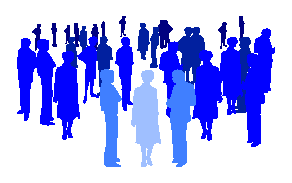
\includegraphics[scale=0.5]{img/estimacion/poblacion}}
\rput(10,7){Población}
\uncover<2->{
\psline{->}(4.5,6.2)(1.2,5.2)
\rput(1,5){$X_1$}
\rput(1,4){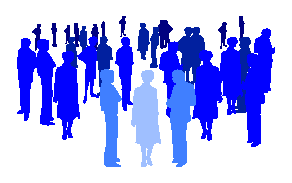
\includegraphics[scale=0.5]{img/estimacion/poblacion}}
\psline{->}(4.5,6.2)(4,5.2)
\rput(4,5){$X_2$}
\rput(4,4){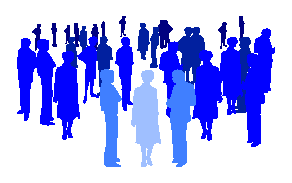
\includegraphics[scale=0.5]{img/estimacion/poblacion}}
\rput(6,4.2){$n$ copias}
\rput(6,4){$\ldots$}
\psline{->}(4.5,6.2)(7.8,5.2)
\rput(8,5){$X_n$}
\rput(8,4){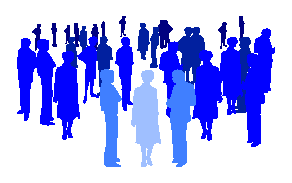
\includegraphics[scale=0.5]{img/estimacion/poblacion}}
\rput(10,5){Variable}
\rput(10,4.5){aleatoria}
\rput(10,4){muestral}
}
\uncover<3->{
\psline{->}(1,3)(1,2)
\rput(0.5,1){$x_1$}
\rput(1,1){
\includegraphics[scale=0.45]{img/estimacion/individuo1}}
\psline{->}(4,3)(4,2)
\rput(3.5,1){$x_2$}
\rput(4,1){
\includegraphics[scale=0.45]{img/estimacion/individuo2}}
\rput(6,1){$\ldots$}
\psline{->}(8,3)(8,2)
\rput(7.5,1){$x_n$}
\rput(8,1){\includegraphics[scale=0.45]{img/estimacion/individuo3}}
\rput(10,1){Muestra}
}
\end{pspicture}
\end{center}
\end{frame}


%---------------------------------------------------------------------slide----
\begin{frame}
\frametitle{Estimación de parámetros}
Las tres cuestiones fundamentales respecto a la variable aleatoria muestral son:
\begin{description}
\item [Homogeneidad]: Las $n$ variables que componen la variable aleatoria muestral siguen la misma distribución.
\item [Independencia]: Las variables son independientes entre sí.
\item [Modelo de distribución]: El modelo de distribución que siguen las $n$ variables.
\end{description}
Las dos primeras cuestiones pueden resolverse si se utiliza muestreo aleatorio simple para obtener la muestra. En cuanto a la última, hay que responder, a su vez, a dos cuestiones:
\begin{itemize}
\item ¿Qué modelo de distribución se ajusta mejor a nuestro conjunto de datos? Esto se resolverá, en parte, mediante la utilización de técnicas no paramétricas.
\item Una vez seleccionado el modelo de distribución más apropiado, ¿qué estadístico del modelo nos interesa y cómo determinar su valor? 
De esto último se encarga la parte de la inferencia estadística conocida como \structure{\textbf{Estimación de Parámetros}}.
\end{itemize}
\end{frame}


%---------------------------------------------------------------------slide----
\begin{frame}
\frametitle{Parámetros a estimar}
En este tema se abordará la segunda cuestión, es decir, suponiendo que se conoce el modelo de distribución de una población, se intentará estimar los principales parámetros que la definen.
Por ejemplo, los principales parámetros que definen las distribuciones vistas en el tema anterior son:
\begin{center}
\begin{tabular}{|l|c|}
\hline
Distribución & Parámetro \\
\hline\hline
Binomial & $n,p$\\
\hline
Poisson & $\lambda$\\
\hline
Uniforme & $a,b$\\
\hline
Normal & $\mu,\sigma$\\
\hline
Chi-cuadrado & $n$\\
\hline
T-Student & $n$\\
\hline
F-Fisher & $m,n$\\
\hline
\end{tabular}
\end{center}
\end{frame}


%---------------------------------------------------------------------slide----
\begin{frame}
\frametitle{Distribución de la variable aleatoria muestral}
La distribución de probabilidad de los valores de la variable muestral depende claramente de la distribución de probabilidad de los valores de la población.

Ejemplo: Sea una población en la que la cuarta parte de las familias no tienen hijos, la mitad de las familias tiene 1 hijo, y el resto tiene 2 hijos.

\begin{center}
\tikzsetnextfilename{estimacion/distribucion_variable_muestral}
\begin{tikzpicture}
\matrix[column sep=2em, ampersand replacement=\&] {
\node{
$
\begin{array}{|c|c|}
\multicolumn{2}{c}{\mbox{Distribución}}\\
\multicolumn{2}{c}{\mbox{Poblacional}}\\
\hline
X & P(x)\\
\hline\hline
0 & 0.25 \\
\hline
1 & 0.50 \\
\hline
2 & 0.25 \\
\hline
\end{array}
$
};
\&
\node at (0,0) [fill=color1, single arrow, shape border rotate=0, text=white, minimum width=1.1cm, align=left]{Muestras de\\ tamaño 2};
\&
\node{
$
\begin{array}{|c|c|}
\multicolumn{2}{c}{\mbox{Distribución muestral}}\\
\hline
(X_1,X_2) & P(x_1,x_2)\\
\hline\hline
(0,0) & 0.0625 \\
\hline
(0,1) & 0.1250 \\
\hline
(0,2) & 0.0625 \\
\hline
(1,0) & 0.1250 \\
\hline
(1,1) & 0.2500 \\
\hline
(1,2) & 0.1250 \\
\hline
(2,0) & 0.0625 \\
\hline
(2,1) & 0.1250 \\
\hline
(2,2) & 0.0625 \\
\hline
\end{array}
$
}; 
\\
};
\end{tikzpicture}
\end{center}
\end{frame}


%---------------------------------------------------------------------slide----
\begin{frame}
\frametitle{Distribución de un estadístico muestral}
Por ser función de una variable aleatoria, un estadístico en el muestreo es también una variable aleatoria.
Por tanto, su distribución de probabilidad también depende de la distribución de la población y de los parámetros que la determinan ($\mu,\sigma,p,\ldots $).

Ejemplo: Si se toma la media muestral $\bar X$ de las muestras de tamaño 2 del ejemplo anterior, su distribución de probabilidad es
\begin{center}
\tikzsetnextfilename{estimacion/distribucion_media}
\begin{tikzpicture}
\matrix[column sep=2em, ampersand replacement=\&] {
\node{
$
\begin{array}{|c|c|}
\multicolumn{2}{c}{\mbox{Distribución muestral}}\\
\hline
(X_1,X_2) & P(x_1,x_2)\\
\hline\hline
(0,0) & 0.0625 \\
\hline
(0,1) & 0.1250 \\
\hline
(0,2) & 0.0625 \\
\hline
(1,0) & 0.1250 \\
\hline
(1,1) & 0.2500 \\
\hline
(1,2) & 0.1250 \\
\hline
(2,0) & 0.0625 \\
\hline
(2,1) & 0.1250 \\
\hline
(2,2) & 0.0625 \\
\hline
\end{array}
$
};
\&
\node at (0,0) [fill=color1, single arrow, shape border rotate=0, text=white, minimum width=1.1cm, align=left]{$\bar x=\frac{X_1+X_2}{2}$};
\&
\node{
$
\begin{array}{|c|c|}
\multicolumn{2}{c}{\mbox{Distribución}}\\
\multicolumn{2}{c}{\mbox{de $\bar{x}$}}\\
\hline
\bar X & P(x)\\
\hline\hline
0 & 0.0625 \\
\hline
0.5 & 0.2500 \\
\hline
1 & 0.3750 \\
\hline
1.5 & 0.2500\\
\hline
2 & 0.0625 \\
\hline
\end{array}
$
}; 
\\
};
\end{tikzpicture}
\end{center}
\end{frame}

%---------------------------------------------------------------------slide----
\begin{frame}
\frametitle{Distribución de un estadístico muestral}
\begin{center}
\tikzsetnextfilename{estimacion/diagrama_barras_distribucion_poblacion}
\resizebox{0.49\textwidth}{!}{% Created by tikzDevice version 0.10.1 on 2017-09-05 00:50:56
% !TEX encoding = UTF-8 Unicode
\begin{tikzpicture}[x=1pt,y=1pt]
\definecolor{fillColor}{RGB}{255,255,255}
\path[use as bounding box,fill=fillColor,fill opacity=0.00] (0,0) rectangle (361.35,289.08);
\begin{scope}
\path[clip] ( 49.20, 61.20) rectangle (336.15,239.88);
\definecolor{drawColor}{RGB}{5,161,230}

\path[draw=drawColor,line width= 4.0pt,line join=round,line cap=round] ( 59.83, 61.20) -- ( 59.83,142.42);

\path[draw=drawColor,line width= 4.0pt,line join=round,line cap=round] (192.67, 61.20) -- (192.67,223.64);

\path[draw=drawColor,line width= 4.0pt,line join=round,line cap=round] (325.52, 61.20) -- (325.52,142.42);
\end{scope}
\begin{scope}
\path[clip] (  0.00,  0.00) rectangle (361.35,289.08);
\definecolor{drawColor}{RGB}{0,0,0}

\path[draw=drawColor,line width= 0.4pt,line join=round,line cap=round] ( 59.83, 61.20) -- (325.52, 61.20);

\path[draw=drawColor,line width= 0.4pt,line join=round,line cap=round] ( 59.83, 61.20) -- ( 59.83, 55.20);

\path[draw=drawColor,line width= 0.4pt,line join=round,line cap=round] (126.25, 61.20) -- (126.25, 55.20);

\path[draw=drawColor,line width= 0.4pt,line join=round,line cap=round] (192.67, 61.20) -- (192.67, 55.20);

\path[draw=drawColor,line width= 0.4pt,line join=round,line cap=round] (259.10, 61.20) -- (259.10, 55.20);

\path[draw=drawColor,line width= 0.4pt,line join=round,line cap=round] (325.52, 61.20) -- (325.52, 55.20);

\node[text=drawColor,anchor=base,inner sep=0pt, outer sep=0pt, scale=  1.00] at ( 59.83, 45.60) {0.0};

\node[text=drawColor,anchor=base,inner sep=0pt, outer sep=0pt, scale=  1.00] at (126.25, 45.60) {0.5};

\node[text=drawColor,anchor=base,inner sep=0pt, outer sep=0pt, scale=  1.00] at (192.67, 45.60) {1.0};

\node[text=drawColor,anchor=base,inner sep=0pt, outer sep=0pt, scale=  1.00] at (259.10, 45.60) {1.5};

\node[text=drawColor,anchor=base,inner sep=0pt, outer sep=0pt, scale=  1.00] at (325.52, 45.60) {2.0};

\path[draw=drawColor,line width= 0.4pt,line join=round,line cap=round] ( 49.20, 61.20) -- ( 49.20,223.64);

\path[draw=drawColor,line width= 0.4pt,line join=round,line cap=round] ( 49.20, 61.20) -- ( 43.20, 61.20);

\path[draw=drawColor,line width= 0.4pt,line join=round,line cap=round] ( 49.20, 93.69) -- ( 43.20, 93.69);

\path[draw=drawColor,line width= 0.4pt,line join=round,line cap=round] ( 49.20,126.17) -- ( 43.20,126.17);

\path[draw=drawColor,line width= 0.4pt,line join=round,line cap=round] ( 49.20,158.66) -- ( 43.20,158.66);

\path[draw=drawColor,line width= 0.4pt,line join=round,line cap=round] ( 49.20,191.15) -- ( 43.20,191.15);

\path[draw=drawColor,line width= 0.4pt,line join=round,line cap=round] ( 49.20,223.64) -- ( 43.20,223.64);

\node[text=drawColor,rotate= 90.00,anchor=base,inner sep=0pt, outer sep=0pt, scale=  1.00] at ( 40.80, 61.20) {0.0};

\node[text=drawColor,rotate= 90.00,anchor=base,inner sep=0pt, outer sep=0pt, scale=  1.00] at ( 40.80, 93.69) {0.1};

\node[text=drawColor,rotate= 90.00,anchor=base,inner sep=0pt, outer sep=0pt, scale=  1.00] at ( 40.80,126.17) {0.2};

\node[text=drawColor,rotate= 90.00,anchor=base,inner sep=0pt, outer sep=0pt, scale=  1.00] at ( 40.80,158.66) {0.3};

\node[text=drawColor,rotate= 90.00,anchor=base,inner sep=0pt, outer sep=0pt, scale=  1.00] at ( 40.80,191.15) {0.4};

\node[text=drawColor,rotate= 90.00,anchor=base,inner sep=0pt, outer sep=0pt, scale=  1.00] at ( 40.80,223.64) {0.5};

\path[draw=drawColor,line width= 0.4pt,line join=round,line cap=round] ( 49.20, 61.20) --
	(336.15, 61.20) --
	(336.15,239.88) --
	( 49.20,239.88) --
	( 49.20, 61.20);
\end{scope}
\begin{scope}
\path[clip] (  0.00,  0.00) rectangle (361.35,289.08);
\definecolor{drawColor}{RGB}{0,0,0}

\node[text=drawColor,anchor=base,inner sep=0pt, outer sep=0pt, scale=  1.20] at (192.68,260.34) {\bfseries Distribución del número de hijos};

\node[text=drawColor,anchor=base,inner sep=0pt, outer sep=0pt, scale=  1.00] at (192.68, 27.60) {Nº de hijos};

\node[text=drawColor,rotate= 90.00,anchor=base,inner sep=0pt, outer sep=0pt, scale=  1.00] at ( 22.80,150.54) {Probabilidad};
\end{scope}
\end{tikzpicture}
}
\tikzsetnextfilename{estimacion/diagrama_barras_distribucion_media}
\resizebox{0.49\textwidth}{!}{% Created by tikzDevice version 0.10.1 on 2017-09-05 00:50:56
% !TEX encoding = UTF-8 Unicode
\begin{tikzpicture}[x=1pt,y=1pt]
\definecolor{fillColor}{RGB}{255,255,255}
\path[use as bounding box,fill=fillColor,fill opacity=0.00] (0,0) rectangle (361.35,289.08);
\begin{scope}
\path[clip] ( 49.20, 61.20) rectangle (336.15,239.88);
\definecolor{drawColor}{RGB}{5,161,230}

\path[draw=drawColor,line width= 4.0pt,line join=round,line cap=round] ( 59.83, 61.20) -- ( 59.83, 81.50);

\path[draw=drawColor,line width= 4.0pt,line join=round,line cap=round] (126.25, 61.20) -- (126.25,142.42);

\path[draw=drawColor,line width= 4.0pt,line join=round,line cap=round] (192.67, 61.20) -- (192.67,183.03);

\path[draw=drawColor,line width= 4.0pt,line join=round,line cap=round] (259.10, 61.20) -- (259.10,142.42);

\path[draw=drawColor,line width= 4.0pt,line join=round,line cap=round] (325.52, 61.20) -- (325.52, 81.50);
\end{scope}
\begin{scope}
\path[clip] (  0.00,  0.00) rectangle (361.35,289.08);
\definecolor{drawColor}{RGB}{0,0,0}

\path[draw=drawColor,line width= 0.4pt,line join=round,line cap=round] ( 59.83, 61.20) -- (325.52, 61.20);

\path[draw=drawColor,line width= 0.4pt,line join=round,line cap=round] ( 59.83, 61.20) -- ( 59.83, 55.20);

\path[draw=drawColor,line width= 0.4pt,line join=round,line cap=round] (126.25, 61.20) -- (126.25, 55.20);

\path[draw=drawColor,line width= 0.4pt,line join=round,line cap=round] (192.67, 61.20) -- (192.67, 55.20);

\path[draw=drawColor,line width= 0.4pt,line join=round,line cap=round] (259.10, 61.20) -- (259.10, 55.20);

\path[draw=drawColor,line width= 0.4pt,line join=round,line cap=round] (325.52, 61.20) -- (325.52, 55.20);

\node[text=drawColor,anchor=base,inner sep=0pt, outer sep=0pt, scale=  1.00] at ( 59.83, 45.60) {0.0};

\node[text=drawColor,anchor=base,inner sep=0pt, outer sep=0pt, scale=  1.00] at (126.25, 45.60) {0.5};

\node[text=drawColor,anchor=base,inner sep=0pt, outer sep=0pt, scale=  1.00] at (192.67, 45.60) {1.0};

\node[text=drawColor,anchor=base,inner sep=0pt, outer sep=0pt, scale=  1.00] at (259.10, 45.60) {1.5};

\node[text=drawColor,anchor=base,inner sep=0pt, outer sep=0pt, scale=  1.00] at (325.52, 45.60) {2.0};

\path[draw=drawColor,line width= 0.4pt,line join=round,line cap=round] ( 49.20, 61.20) -- ( 49.20,223.64);

\path[draw=drawColor,line width= 0.4pt,line join=round,line cap=round] ( 49.20, 61.20) -- ( 43.20, 61.20);

\path[draw=drawColor,line width= 0.4pt,line join=round,line cap=round] ( 49.20, 93.69) -- ( 43.20, 93.69);

\path[draw=drawColor,line width= 0.4pt,line join=round,line cap=round] ( 49.20,126.17) -- ( 43.20,126.17);

\path[draw=drawColor,line width= 0.4pt,line join=round,line cap=round] ( 49.20,158.66) -- ( 43.20,158.66);

\path[draw=drawColor,line width= 0.4pt,line join=round,line cap=round] ( 49.20,191.15) -- ( 43.20,191.15);

\path[draw=drawColor,line width= 0.4pt,line join=round,line cap=round] ( 49.20,223.64) -- ( 43.20,223.64);

\node[text=drawColor,rotate= 90.00,anchor=base,inner sep=0pt, outer sep=0pt, scale=  1.00] at ( 40.80, 61.20) {0.0};

\node[text=drawColor,rotate= 90.00,anchor=base,inner sep=0pt, outer sep=0pt, scale=  1.00] at ( 40.80, 93.69) {0.1};

\node[text=drawColor,rotate= 90.00,anchor=base,inner sep=0pt, outer sep=0pt, scale=  1.00] at ( 40.80,126.17) {0.2};

\node[text=drawColor,rotate= 90.00,anchor=base,inner sep=0pt, outer sep=0pt, scale=  1.00] at ( 40.80,158.66) {0.3};

\node[text=drawColor,rotate= 90.00,anchor=base,inner sep=0pt, outer sep=0pt, scale=  1.00] at ( 40.80,191.15) {0.4};

\node[text=drawColor,rotate= 90.00,anchor=base,inner sep=0pt, outer sep=0pt, scale=  1.00] at ( 40.80,223.64) {0.5};

\path[draw=drawColor,line width= 0.4pt,line join=round,line cap=round] ( 49.20, 61.20) --
	(336.15, 61.20) --
	(336.15,239.88) --
	( 49.20,239.88) --
	( 49.20, 61.20);
\end{scope}
\begin{scope}
\path[clip] (  0.00,  0.00) rectangle (361.35,289.08);
\definecolor{drawColor}{RGB}{0,0,0}

\node[text=drawColor,anchor=base,inner sep=0pt, outer sep=0pt, scale=  1.20] at (192.68,260.34) {\bfseries Distribución de $\bar x$};

\node[text=drawColor,anchor=base west,inner sep=0pt, outer sep=0pt, scale=  1.00] at (190.04, 27.60) {x};

\path[draw=drawColor,line width= 0.4pt,line join=round,line cap=round] (190.04, 33.28) --
	(195.31, 33.28);

\node[text=drawColor,rotate= 90.00,anchor=base,inner sep=0pt, outer sep=0pt, scale=  1.00] at ( 22.80,150.54) {Probabilidad};
\end{scope}
\end{tikzpicture}
}

\emph{¿Cuál es la probabilidad de obtener una media muestral que aproxime la media poblacional con un error máximo de 0.5?}
\end{center}
\end{frame}


%---------------------------------------------------------------------slide----
\begin{frame}
\frametitle{Teorema central del límite}
Como hemos visto, para conocer la distribución de un estadístico muestral, es necesario conocer la distribución de la población, lo cual no siempre es posible. 
Afortunadamente, para muestras grandes es posible aproximar la distribución de algunos estadísticos como la media, gracias al siguiente teorema:

\begin{teorema}[Teorema central del límite]
Si $X_1,\ldots, X_n$ son variables aleatorias independientes  ($n\geq 30$) con medias y varianzas $\mu_i=E(X_i)$, $\sigma^2_i=Var(X_i)$, $i=1,\ldots,n$ respectivamente, entonces la variable aleatoria $X=X_1+\cdots+X_n$ sigue una distribución aproximadamente normal de media la suma de las medias y varianza la suma de las varianzas
\[
X=X_1+\cdots+X_n\stackrel{n\geq 30} \sim N\left(\sum_{i=1}^n \mu_i, \sqrt{\sum_{i=1}^n \sigma^2_i}\right)
\]
\end{teorema}

Este teorema además es la explicación de que la mayoría de las variables biológicas presenten una distribución normal, ya que suelen ser causa de múltiples factores que suman sus efectos de manera independiente.
\end{frame}


%---------------------------------------------------------------------slide----
\begin{frame}
\frametitle{Distribución de la media muestral}
\framesubtitle{Muestras grandes ($n\geq 30$)}
La media muestral de una muestra aleatoria de tamaño $n$ es la suma de $n$ variables aleatorias independientes, idénticamente distribuidas:
\[
\bar X = \frac{X_1+\cdots+X_n}{n} = \frac{X_1}{n}+\cdots+\frac{X_n}{n}
\]
De acuerdo a las propiedades de las transformaciones lineales, la media y la varianza de cada una de estas variables son
\[
E\left(\frac{X_i}{n}\right) =\frac{\mu}{n} \quad  \mbox{y} \quad Var\left(\frac{X_i}{n}\right) = \frac{\sigma^2}{n^2}
\]
con $\mu$ y $\sigma^2$ la media y la varianza de la población de partida.

Entonces, si el tamaño de la muestra es grande ($n\geq 30$), de acuerdo al teorema central del límite, la distribución de la media muestral será normal:
\[
\bar X \sim N\left(\sum_{i=1}^n \frac{\mu}{n},\sqrt{\sum_{i=1}^n \frac{\sigma^2}{n^2}} \right) = N\left(\mu,\frac{\sigma}{\sqrt{n}} \right).
\]
\end{frame}


%---------------------------------------------------------------------slide----
\begin{frame}
\frametitle{Distribución de la media muestral}
\framesubtitle{Ejemplo para muestras grandes ($n\geq 30$)}
Supongase que se desea estimar el número medio de hijos de una población con media $\mu=2$ hijos y desviación típica $\sigma=1$ hijo.
\begin{center}
\emph{¿Qué probabilidad hay de estimar $\mu$ a partir de $\bar x$ con un error menor de $0.2$?}
\end{center}
\begin{columns}
\begin{column}{0.5\textwidth}
De acuerdo al teorema central del límite se tiene:
\begin{itemize}
\item Para $n=30$, $\bar x\sim N(2,1/\sqrt{30})$ y
\[
P(1.8<\bar x<2.2) = 0.7267.
\]

\item Para $n=100$, $\bar x\sim N(2,1/\sqrt{100})$ y
\[
P(1.8<\bar x<2.2) = 0.9545.
\]
\end{itemize}
\end{column}
\begin{column}{0.5\textwidth}
\begin{center}
\tikzsetnextfilename{estimacion/teorema_central_limite}
\resizebox{0.9\textwidth}{!}{% Created by tikzDevice version 0.10.1 on 2017-09-05 18:24:29
% !TEX encoding = UTF-8 Unicode
\begin{tikzpicture}[x=1pt,y=1pt]
\definecolor{fillColor}{RGB}{255,255,255}
\path[use as bounding box,fill=fillColor,fill opacity=0.00] (0,0) rectangle (289.08,252.94);
\begin{scope}
\path[clip] ( 36.00, 36.00) rectangle (277.08,216.94);
\definecolor{drawColor}{RGB}{5,161,230}

\path[draw=drawColor,line width= 0.4pt,line join=round,line cap=round] ( 44.93, 36.00) --
	( 46.43, 36.00) --
	( 47.93, 36.00) --
	( 49.42, 36.00) --
	( 50.92, 36.00) --
	( 52.42, 36.00) --
	( 53.92, 36.00) --
	( 55.42, 36.00) --
	( 56.91, 36.00) --
	( 58.41, 36.00) --
	( 59.91, 36.00) --
	( 61.41, 36.00) --
	( 62.91, 36.00) --
	( 64.40, 36.00) --
	( 65.90, 36.00) --
	( 67.40, 36.00) --
	( 68.90, 36.00) --
	( 70.40, 36.00) --
	( 71.90, 36.00) --
	( 73.39, 36.00) --
	( 74.89, 36.00) --
	( 76.39, 36.00) --
	( 77.89, 36.00) --
	( 79.39, 36.00) --
	( 80.88, 36.00) --
	( 82.38, 36.00) --
	( 83.88, 36.00) --
	( 85.38, 36.00) --
	( 86.88, 36.00) --
	( 88.37, 36.00) --
	( 89.87, 36.00) --
	( 91.37, 36.00) --
	( 92.87, 36.00) --
	( 94.37, 36.00) --
	( 95.87, 36.00) --
	( 97.36, 36.00) --
	( 98.86, 36.00) --
	(100.36, 36.00) --
	(101.86, 36.00) --
	(103.36, 36.00) --
	(104.85, 36.00) --
	(106.35, 36.01) --
	(107.85, 36.01) --
	(109.35, 36.02) --
	(110.85, 36.04) --
	(112.34, 36.07) --
	(113.84, 36.11) --
	(115.34, 36.19) --
	(116.84, 36.31) --
	(118.34, 36.49) --
	(119.84, 36.77) --
	(121.33, 37.19) --
	(122.83, 37.80) --
	(124.33, 38.67) --
	(125.83, 39.90) --
	(127.33, 41.59) --
	(128.82, 43.87) --
	(130.32, 46.89) --
	(131.82, 50.79) --
	(133.32, 55.74) --
	(134.82, 61.86) --
	(136.32, 69.28) --
	(137.81, 78.06) --
	(139.31, 88.21) --
	(140.81, 99.66) --
	(142.31,112.23) --
	(143.81,125.65) --
	(145.30,139.55) --
	(146.80,153.47) --
	(148.30,166.88) --
	(149.80,179.21) --
	(151.30,189.91) --
	(152.79,198.46) --
	(154.29,204.42) --
	(155.79,207.49) --
	(157.29,207.49) --
	(158.79,204.42) --
	(160.29,198.46) --
	(161.78,189.91) --
	(163.28,179.21) --
	(164.78,166.88) --
	(166.28,153.47) --
	(167.78,139.55) --
	(169.27,125.65) --
	(170.77,112.23) --
	(172.27, 99.66) --
	(173.77, 88.21) --
	(175.27, 78.06) --
	(176.76, 69.28) --
	(178.26, 61.86) --
	(179.76, 55.74) --
	(181.26, 50.79) --
	(182.76, 46.89) --
	(184.26, 43.87) --
	(185.75, 41.59) --
	(187.25, 39.90) --
	(188.75, 38.67) --
	(190.25, 37.80) --
	(191.75, 37.19) --
	(193.24, 36.77) --
	(194.74, 36.49) --
	(196.24, 36.31) --
	(197.74, 36.19) --
	(199.24, 36.11) --
	(200.74, 36.07) --
	(202.23, 36.04) --
	(203.73, 36.02) --
	(205.23, 36.01) --
	(206.73, 36.01) --
	(208.23, 36.00) --
	(209.72, 36.00) --
	(211.22, 36.00) --
	(212.72, 36.00) --
	(214.22, 36.00) --
	(215.72, 36.00) --
	(217.21, 36.00) --
	(218.71, 36.00) --
	(220.21, 36.00) --
	(221.71, 36.00) --
	(223.21, 36.00) --
	(224.71, 36.00) --
	(226.20, 36.00) --
	(227.70, 36.00) --
	(229.20, 36.00) --
	(230.70, 36.00) --
	(232.20, 36.00) --
	(233.69, 36.00) --
	(235.19, 36.00) --
	(236.69, 36.00) --
	(238.19, 36.00) --
	(239.69, 36.00) --
	(241.18, 36.00) --
	(242.68, 36.00) --
	(244.18, 36.00) --
	(245.68, 36.00) --
	(247.18, 36.00) --
	(248.68, 36.00) --
	(250.17, 36.00) --
	(251.67, 36.00) --
	(253.17, 36.00) --
	(254.67, 36.00) --
	(256.17, 36.00) --
	(257.66, 36.00) --
	(259.16, 36.00) --
	(260.66, 36.00) --
	(262.16, 36.00) --
	(263.66, 36.00) --
	(265.15, 36.00) --
	(266.65, 36.00) --
	(268.15, 36.00);
\end{scope}
\begin{scope}
\path[clip] (  0.00,  0.00) rectangle (289.08,252.94);
\definecolor{drawColor}{RGB}{0,0,0}

\path[draw=drawColor,line width= 0.4pt,line join=round,line cap=round] ( 44.93, 36.00) -- (268.15, 36.00);

\path[draw=drawColor,line width= 0.4pt,line join=round,line cap=round] ( 44.93, 36.00) -- ( 44.93, 30.00);

\path[draw=drawColor,line width= 0.4pt,line join=round,line cap=round] (100.73, 36.00) -- (100.73, 30.00);

\path[draw=drawColor,line width= 0.4pt,line join=round,line cap=round] (156.54, 36.00) -- (156.54, 30.00);

\path[draw=drawColor,line width= 0.4pt,line join=round,line cap=round] (212.35, 36.00) -- (212.35, 30.00);

\path[draw=drawColor,line width= 0.4pt,line join=round,line cap=round] (268.15, 36.00) -- (268.15, 30.00);

\node[text=drawColor,anchor=base,inner sep=0pt, outer sep=0pt, scale=  1.00] at ( 44.93, 20.40) {1.0};

\node[text=drawColor,anchor=base,inner sep=0pt, outer sep=0pt, scale=  1.00] at (100.73, 20.40) {1.5};

\node[text=drawColor,anchor=base,inner sep=0pt, outer sep=0pt, scale=  1.00] at (156.54, 20.40) {2.0};

\node[text=drawColor,anchor=base,inner sep=0pt, outer sep=0pt, scale=  1.00] at (212.35, 20.40) {2.5};

\node[text=drawColor,anchor=base,inner sep=0pt, outer sep=0pt, scale=  1.00] at (268.15, 20.40) {3.0};

\path[draw=drawColor,line width= 0.4pt,line join=round,line cap=round] ( 36.00, 36.00) -- ( 36.00,208.33);

\path[draw=drawColor,line width= 0.4pt,line join=round,line cap=round] ( 36.00, 36.00) -- ( 30.00, 36.00);

\path[draw=drawColor,line width= 0.4pt,line join=round,line cap=round] ( 36.00, 79.08) -- ( 30.00, 79.08);

\path[draw=drawColor,line width= 0.4pt,line join=round,line cap=round] ( 36.00,122.16) -- ( 30.00,122.16);

\path[draw=drawColor,line width= 0.4pt,line join=round,line cap=round] ( 36.00,165.25) -- ( 30.00,165.25);

\path[draw=drawColor,line width= 0.4pt,line join=round,line cap=round] ( 36.00,208.33) -- ( 30.00,208.33);

\node[text=drawColor,rotate= 90.00,anchor=base,inner sep=0pt, outer sep=0pt, scale=  1.00] at ( 27.60, 36.00) {0};

\node[text=drawColor,rotate= 90.00,anchor=base,inner sep=0pt, outer sep=0pt, scale=  1.00] at ( 27.60, 79.08) {1};

\node[text=drawColor,rotate= 90.00,anchor=base,inner sep=0pt, outer sep=0pt, scale=  1.00] at ( 27.60,122.16) {2};

\node[text=drawColor,rotate= 90.00,anchor=base,inner sep=0pt, outer sep=0pt, scale=  1.00] at ( 27.60,165.25) {3};

\node[text=drawColor,rotate= 90.00,anchor=base,inner sep=0pt, outer sep=0pt, scale=  1.00] at ( 27.60,208.33) {4};

\path[draw=drawColor,line width= 0.4pt,line join=round,line cap=round] ( 36.00, 36.00) --
	(277.08, 36.00) --
	(277.08,216.94) --
	( 36.00,216.94) --
	( 36.00, 36.00);
\end{scope}
\begin{scope}
\path[clip] (  0.00,  0.00) rectangle (289.08,252.94);
\definecolor{drawColor}{RGB}{0,0,0}

\node[text=drawColor,anchor=base,inner sep=0pt, outer sep=0pt, scale=  1.20] at (156.54,230.80) {\bfseries Distribuciones de la media del nº de hijos};

\node[text=drawColor,anchor=base,inner sep=0pt, outer sep=0pt, scale=  1.00] at (156.54,  2.40) {$\bar x$};

\node[text=drawColor,rotate= 90.00,anchor=base,inner sep=0pt, outer sep=0pt, scale=  1.00] at (  9.60,126.47) {Densidad $f(x)$};
\end{scope}
\begin{scope}
\path[clip] ( 36.00, 36.00) rectangle (277.08,216.94);
\definecolor{drawColor}{RGB}{238,50,36}

\path[draw=drawColor,line width= 0.4pt,line join=round,line cap=round] ( 44.93, 36.00) --
	( 46.43, 36.00) --
	( 47.93, 36.00) --
	( 49.42, 36.00) --
	( 50.92, 36.00) --
	( 52.42, 36.00) --
	( 53.92, 36.00) --
	( 55.42, 36.00) --
	( 56.91, 36.00) --
	( 58.41, 36.00) --
	( 59.91, 36.00) --
	( 61.41, 36.00) --
	( 62.91, 36.00) --
	( 64.40, 36.00) --
	( 65.90, 36.00) --
	( 67.40, 36.01) --
	( 68.90, 36.01) --
	( 70.40, 36.01) --
	( 71.90, 36.02) --
	( 73.39, 36.02) --
	( 74.89, 36.03) --
	( 76.39, 36.04) --
	( 77.89, 36.05) --
	( 79.39, 36.07) --
	( 80.88, 36.10) --
	( 82.38, 36.13) --
	( 83.88, 36.16) --
	( 85.38, 36.21) --
	( 86.88, 36.27) --
	( 88.37, 36.35) --
	( 89.87, 36.45) --
	( 91.37, 36.57) --
	( 92.87, 36.71) --
	( 94.37, 36.90) --
	( 95.87, 37.12) --
	( 97.36, 37.39) --
	( 98.86, 37.71) --
	(100.36, 38.10) --
	(101.86, 38.57) --
	(103.36, 39.12) --
	(104.85, 39.77) --
	(106.35, 40.53) --
	(107.85, 41.42) --
	(109.35, 42.44) --
	(110.85, 43.62) --
	(112.34, 44.96) --
	(113.84, 46.48) --
	(115.34, 48.19) --
	(116.84, 50.11) --
	(118.34, 52.24) --
	(119.84, 54.59) --
	(121.33, 57.16) --
	(122.83, 59.96) --
	(124.33, 62.99) --
	(125.83, 66.24) --
	(127.33, 69.69) --
	(128.82, 73.33) --
	(130.32, 77.15) --
	(131.82, 81.10) --
	(133.32, 85.18) --
	(134.82, 89.33) --
	(136.32, 93.53) --
	(137.81, 97.71) --
	(139.31,101.85) --
	(140.81,105.88) --
	(142.31,109.76) --
	(143.81,113.44) --
	(145.30,116.86) --
	(146.80,119.98) --
	(148.30,122.75) --
	(149.80,125.13) --
	(151.30,127.07) --
	(152.79,128.56) --
	(154.29,129.57) --
	(155.79,130.08) --
	(157.29,130.08) --
	(158.79,129.57) --
	(160.29,128.56) --
	(161.78,127.07) --
	(163.28,125.13) --
	(164.78,122.75) --
	(166.28,119.98) --
	(167.78,116.86) --
	(169.27,113.44) --
	(170.77,109.76) --
	(172.27,105.88) --
	(173.77,101.85) --
	(175.27, 97.71) --
	(176.76, 93.53) --
	(178.26, 89.33) --
	(179.76, 85.18) --
	(181.26, 81.10) --
	(182.76, 77.15) --
	(184.26, 73.33) --
	(185.75, 69.69) --
	(187.25, 66.24) --
	(188.75, 62.99) --
	(190.25, 59.96) --
	(191.75, 57.16) --
	(193.24, 54.59) --
	(194.74, 52.24) --
	(196.24, 50.11) --
	(197.74, 48.19) --
	(199.24, 46.48) --
	(200.74, 44.96) --
	(202.23, 43.62) --
	(203.73, 42.44) --
	(205.23, 41.42) --
	(206.73, 40.53) --
	(208.23, 39.77) --
	(209.72, 39.12) --
	(211.22, 38.57) --
	(212.72, 38.10) --
	(214.22, 37.71) --
	(215.72, 37.39) --
	(217.21, 37.12) --
	(218.71, 36.90) --
	(220.21, 36.71) --
	(221.71, 36.57) --
	(223.21, 36.45) --
	(224.71, 36.35) --
	(226.20, 36.27) --
	(227.70, 36.21) --
	(229.20, 36.16) --
	(230.70, 36.13) --
	(232.20, 36.10) --
	(233.69, 36.07) --
	(235.19, 36.05) --
	(236.69, 36.04) --
	(238.19, 36.03) --
	(239.69, 36.02) --
	(241.18, 36.02) --
	(242.68, 36.01) --
	(244.18, 36.01) --
	(245.68, 36.01) --
	(247.18, 36.00) --
	(248.68, 36.00) --
	(250.17, 36.00) --
	(251.67, 36.00) --
	(253.17, 36.00) --
	(254.67, 36.00) --
	(256.17, 36.00) --
	(257.66, 36.00) --
	(259.16, 36.00) --
	(260.66, 36.00) --
	(262.16, 36.00) --
	(263.66, 36.00) --
	(265.15, 36.00) --
	(266.65, 36.00) --
	(268.15, 36.00);
\definecolor{drawColor}{RGB}{5,161,230}

\path[draw=drawColor,line width= 0.4pt,line join=round,line cap=round] (217.25,204.94) -- (235.25,204.94);
\definecolor{drawColor}{RGB}{238,50,36}

\path[draw=drawColor,line width= 0.4pt,line join=round,line cap=round] (217.25,192.94) -- (235.25,192.94);
\definecolor{drawColor}{RGB}{0,0,0}

\node[text=drawColor,anchor=base west,inner sep=0pt, outer sep=0pt, scale=  1.00] at (244.25,201.50) {n=100};

\node[text=drawColor,anchor=base west,inner sep=0pt, outer sep=0pt, scale=  1.00] at (244.25,189.50) {n=30};
\end{scope}
\end{tikzpicture}
}
\end{center}
\end{column}
\end{columns}
\end{frame}


%---------------------------------------------------------------------slide----
\begin{frame}
\frametitle{Distribución de una proporción muestral}
\framesubtitle{Muestras grandes ($n\geq 30$)}
Una proporción $p$ poblacional puede calcularse como la media de una variable dicotómica (0,1).
Esta variable se conoce como \emph{variable de Bernouilli} $B(p)$, que es un caso particular de la binomial para $n=1$.
Por tanto, para una muestra aleatoria de tamaño $n$, una proporción muestral $\hat p$ también puede expresarse como la suma de $n$ variables aleatorias independientes, idénticamente distribuidas:
\[
\hat p = \bar X = \frac{X_1+\cdots+X_n}{n} = \frac{X_1}{n}+\cdots+\frac{X_n}{n}, \mbox{ con } X_i\sim B(p)
\]
y con media y varianza
\[
E\left(\frac{X_i}{n}\right) =\frac{p}{n} \quad  \mbox{y} \quad Var\left(\frac{X_i}{n}\right) = \frac{p(1-p)}{n^2}
\]

Entonces, si el tamaño de la muestra es grande ($n\geq 30$), de acuerdo al teorema central del límite, la distribución de la proporción muestral también será normal:
\[
\hat p \sim N\left(\sum_{i=1}^n \frac{p}{n},\sqrt{\sum_{i=1}^n \frac{p(1-p)}{n^2}} \right) = N\left(p,\sqrt{\frac{p(1-p)}{n}} \right).
\]
\end{frame}


\subsection{Estimadores}
%---------------------------------------------------------------------slide----
\begin{frame}
\frametitle{Estimador y estimación}
Los estadísticos muestrales pueden utilizarse para aproximar los parámetros de la población, y cuando un estadístico se utiliza con este fin se le llama \emph{estimador del parámetro}.
\begin{definicion}[Estimador y estimación]
Un \emph{estimador} es una función de la variable aleatoria muestral
\[
\hat \theta = F(X_1,\ldots,X_n).
\]
Dada una muestra concreta $(x_1,\ldots,x_n)$, el valor del estimador aplicado a ella se conoce como \emph{estimación}
\[
\hat \theta_0 = F(x_1,\ldots,x_n).
\]
\end{definicion}

Por ser una función de la variable aleatoria muestral, un estimador es, a su vez, una variable aleatoria cuya distribución depende de la población de partida.

Mientras que el estimador es una función que es única, la estimación no es única, sino que depende de la muestra tomada.
\end{frame}


%---------------------------------------------------------------------slide----
\begin{frame}
\frametitle{Estimador y estimación}
\begin{center}
\tikzsetnextfilename{estimacion/estimador_estimacion}
% Autor: Alfredo Sánchez Alberca (email:asalber@ceu.es)
% Gráfico que muestra la diferencia entre estimador y estimación 
\begin{tikzpicture}
\tikzstyle{node} = [align=center, node distance=1cm, text=color1]; 
\tikzstyle{arrow} = [fill=color1, single arrow, shape border rotate=0, text=white, minimum width=1.1cm, align=left];

\node at (0,5) {Distribución de la población}; 
\node at (0,4.5) {$X$}; 
\pause
\node at (3,4.5) [arrow]{Parámetro poblacional};
\node (parametro) at (6,4.5) {¿$\theta$?};
\pause
\draw[-latex, color1, line width=2pt] (0,4) -- (0,3); 
\node at (0,2.5) {Variable aleatoria muestral}; 
\node at (0,2) {$(X_1,\ldots,X_n)$};
\pause
\node at (3,2) [arrow]{Estimador};
\node at (6,2) {$\hat\theta=F(X_1,\ldots,X_n)$}; 
\pause
\draw[-latex, color1, line width=2pt] (0,1.5) -- (0,0.5); 
\node at (0,0) {Muestra de tamaño $n$}; 
\node at (0,-0.5) {$(x_1,\ldots,x_n)$};
\pause
\node at (3,-0.5) [arrow]{Estimación};
\node (estimacion) at (6,-0.5) {$\hat\theta_0=F(x_1,\ldots,x_n)$}; 
\pause
\draw [-latex, color1, line width=2pt] (estimacion.northeast) to [out=30,in=-30] (parametro.southeast);
\end{tikzpicture} 
\end{center}
\end{frame}


%---------------------------------------------------------------------slide----
\begin{frame}
\frametitle{Estimador y estimación}
\framesubtitle{Ejemplo}
Supóngase que se quiere saber la proporción $p$ de fumadores en una ciudad.
En ese caso, la variable dicotómica que mide si una persona fuma (1) o no (0), sigue una distribución de Bernouilli $B(p)$.

Si se toma una muestra aleatoria de tamaño 5, $(X_1,X_2,X_3,X_4,X_5)$, de esta población, se puede utilizar la proporción de fumadores en la muestra como estimador para la proporción de fumadores en la población:
\[
\hat p = \frac{\sum_{i=1}^5 X_i}{5}
\]
Este estimador es una variable que se distribuye
$\hat p\sim \frac{1}{n}B\left(p,\sqrt{\frac{p(1-p)}{n}}\right)$.

Si se toman distintas muestras, se obtienen diferentes estimaciones:
\[
\begin{array}{|c|c|}
\hline
\mbox{Muestra} & \mbox{Estimación}\\
\hline\hline
(1, 0, 0, 1, 1) & 3/5\\
\hline
(1, 0, 0, 0, 0) & 1/5\\
\hline
(0, 1, 0, 0, 1) & 2/5\\
\hline
\cdots & \cdots\\
\hline
\end{array}
\]
\end{frame}


%---------------------------------------------------------------------slide----
\begin{frame}
\frametitle{Tipos de estimación}
La estimación de parámetros puede realizar de de dos formas:
\begin{description}
\item[Estimación puntual]: Se utiliza un único estimador que proporciona un valor o estimación aproximada del parámetro.
El principal inconveniente de este tipo de estimación es que no se especifica la bondad de la estimación.
\item[Estimación por intervalos]: Se utilizan dos estimadores que proporcionan los extremos de un intervalo dentro del cual se cree que está el verdadero valor del parámetro con un cierto grado de seguridad.
Esta forma de estimar sí permite controlar el error cometido en la estimación.
\end{description}

\begin{center}
\tikzsetnextfilename{estimacion/estimacion_puntual_intervalo}
\begin{tikzpicture}
\node at (1.5,1) {Estimación puntual};
\draw (0,0.5) -- (3,0.5);
\draw (1.5,0.6) -- (1.5,0.4);
\node at (1.5,0) {$\theta$};
\draw[color=color2] (2,0.6) -- (2,0.4);
\node[color=color2] at (2,0) {$\hat\theta_0$};
\node at (7.5,1) {Estimación por intervalo};
\draw (6,0.5) -- (9,0.5);
\draw (7.5,0.6) -- (7.5,0.4);
\node at (7.5,0) {$\theta$};
\node[color=color2] at (7,0.5) {[};
\node[color=color2] at (8.2,0.5) {]};
\node[color=color2] at (7,0) {$l_1$};
\node[color=color2] at (8.2,0) {$l_2$};
\end{tikzpicture}
\end{center}
\end{frame}


\subsection{Estimación puntual}
%---------------------------------------------------------------------slide----
\begin{frame}
\frametitle{Estimación puntual}
La estimación puntual utiliza un único estimador para estimar el valor del parámetro desconocido de la población.

En teoría pueden utilizarse distintos estimadores para estimar un mismo parámetro. Por ejemplo, en el caso de estimar la proporción de fumadores en una ciudad, podrían haberse utilizado otros posibles estimadores además de la proporción muestral, como pueden ser:
\begin{align*}
\hat \theta_1 &= \sqrt[5]{X_1X_2X_3X_4X_5}\\
\hat \theta_2 &= \frac{X_1+X_5}{2}\\
\hat \theta_3 &= X_1 \cdots
\end{align*}

\begin{center}
\alert{\emph{¿Cuál es el mejor estimador?}}
\end{center}

La respuesta a esta cuestión depende de las propiedades de cada estimador.
\end{frame}


%---------------------------------------------------------------------slide----
\begin{frame}
\frametitle{Propiedades de los estimadores}
Aunque la estimación puntual no proporciona ninguna medida del grado de bondad de la estimación, existen varias propiedades que garantizan dicha bondad.

Las propiedades más deseables en un estimador son:
\begin{itemize}
\item Insesgadez
\item Eficiencia
\item Consistencia
\item Normalidad asintótica
\item Suficiencia
\end{itemize}
\end{frame}


%---------------------------------------------------------------------slide----
\begin{frame}
\frametitle{Insesgadez}
\begin{definicion}[Estimador insesgado]
Un estimador $\hat \theta$ es \emph{insesgado} para un parámetro $\theta$ si su esperanza es precisamente $\theta$, es decir,
\[
E(\hat \theta)=\theta.
\]
\end{definicion}
\begin{center}
\tikzsetnextfilename{estimacion/estimadores_sesgados_insesgados}
\scalebox{0.7}{%% Input file name: estimacion/estimadores_sesgados_insesgados.fig
%% FIG version: 3.2
%% Orientation: Landscape
%% Justification: Flush Left
%% Units: Inches
%% Paper size: Letter
%% Magnification: 100.0
%% Resolution: 1200ppi

\begin{pspicture}(5.97cm,3.71cm)(16.34cm,13.69cm)
\psset{unit=0.8cm}
%%
%% Depth: 2147483647
%%
\newrgbcolor{mycolor0}{1.00 0.50 0.31}\definecolor{mycolor0}{rgb}{1.00,0.50,0.31}
\newrgbcolor{mycolor2}{0.28 0.46 1.00}\definecolor{mycolor2}{rgb}{0.28,0.46,1.00}
\newgray{mycolor3}{0.74}\definecolor{mycolor3}{gray}{0.74}
%%
%% Depth: 100
%%
\psset{linestyle=solid,linewidth=0.03175,linecolor=mycolor0,fillstyle=none}
\psline(10.56,7.09)(10.63,7.10)(10.71,7.11)(10.79,7.12)(10.86,7.14)(10.94,7.16)(11.02,7.18)(11.10,7.21)(11.18,7.24)(11.25,7.27)(11.33,7.32)(11.41,7.37)(11.49,7.42)(11.56,7.49)(11.64,7.56)(11.72,7.65)(11.80,7.74)(11.87,7.85)(11.95,7.97)(12.03,8.10)(12.11,8.25)(12.18,8.42)(12.26,8.60)(12.34,8.79)(12.42,9.00)(12.49,9.23)(12.57,9.47)(12.65,9.73)(12.73,10.01)(12.80,10.29)(12.88,10.59)(12.96,10.90)(13.04,11.22)(13.11,11.54)(13.19,11.87)(13.27,12.20)(13.35,12.53)(13.42,12.86)(13.50,13.17)(13.58,13.48)(13.66,13.77)(13.73,14.04)(13.81,14.29)(13.89,14.52)(13.97,14.72)(14.04,14.89)(14.12,15.03)(14.20,15.14)(14.28,15.21)(14.35,15.25)(14.43,15.25)(14.51,15.21)(14.59,15.14)(14.66,15.03)(14.74,14.89)(14.82,14.72)(14.90,14.52)(14.97,14.29)(15.05,14.04)(15.13,13.77)(15.21,13.48)(15.28,13.17)(15.36,12.86)(15.44,12.53)(15.52,12.20)(15.59,11.87)(15.67,11.54)(15.75,11.22)(15.83,10.90)(15.90,10.59)(15.98,10.29)(16.06,10.01)(16.14,9.73)(16.21,9.47)(16.29,9.23)(16.37,9.00)(16.45,8.79)(16.52,8.60)(16.60,8.42)(16.68,8.25)(16.76,8.10)(16.83,7.97)(16.91,7.85)(16.99,7.74)(17.07,7.65)(17.14,7.56)(17.22,7.49)(17.30,7.42)(17.38,7.37)(17.45,7.32)(17.53,7.27)(17.61,7.24)(17.69,7.21)(17.77,7.18)(17.84,7.16)(17.92,7.14)(18.00,7.12)(18.08,7.11)(18.15,7.10)(18.23,7.09)
\psset{linecolor=black}
\psline(9.36,7.05)(9.36,15.27)
\psline(9.36,7.05)(9.14,7.05)
\psline(9.36,9.11)(9.14,9.11)
\psline(9.36,11.16)(9.14,11.16)
\psline(9.36,13.22)(9.14,13.22)
\psline(9.36,15.27)(9.14,15.27)
\rput[B]{90}(8.85,7.05){0.0}
\rput[B]{90}(8.85,9.11){0.1}
\rput[B]{90}(8.85,11.16){0.2}
\rput[B]{90}(8.85,13.22){0.3}
\rput[B]{90}(8.85,15.27){0.4}
\psline(9.36,6.77)(19.43,6.77)(19.43,15.57)(9.36,15.57)(9.36,6.77)
\rput[B](14.39,16.29){Distribuciones de estimadores sesgados e insesgados}
\rput[B](14.39,5.16){Valores de los estimadores}
\rput[lB]{90}(7.98,9.84){Densidad $f(x)$}
\psset{linestyle=dashed,linecolor=green}
\psline(9.39,7.09)(9.47,7.10)(9.54,7.11)(9.62,7.12)(9.70,7.14)(9.78,7.16)(9.85,7.18)(9.93,7.21)(10.01,7.24)(10.09,7.27)(10.16,7.32)(10.24,7.37)(10.32,7.42)(10.40,7.49)(10.47,7.56)(10.55,7.65)(10.63,7.74)(10.71,7.85)(10.78,7.97)(10.86,8.10)(10.94,8.25)(11.02,8.42)(11.09,8.60)(11.17,8.79)(11.25,9.00)(11.33,9.23)(11.40,9.47)(11.48,9.73)(11.56,10.01)(11.64,10.29)(11.71,10.59)(11.79,10.90)(11.87,11.22)(11.95,11.54)(12.02,11.87)(12.10,12.20)(12.18,12.53)(12.26,12.86)(12.33,13.17)(12.41,13.48)(12.49,13.77)(12.57,14.04)(12.64,14.29)(12.72,14.52)(12.80,14.72)(12.88,14.89)(12.95,15.03)(13.03,15.14)(13.11,15.21)(13.19,15.25)(13.27,15.25)(13.34,15.21)(13.42,15.14)(13.50,15.03)(13.58,14.89)(13.65,14.72)(13.73,14.52)(13.81,14.29)(13.89,14.04)(13.96,13.77)(14.04,13.48)(14.12,13.17)(14.20,12.86)(14.27,12.53)(14.35,12.20)(14.43,11.87)(14.51,11.54)(14.58,11.22)(14.66,10.90)(14.74,10.59)(14.82,10.29)(14.89,10.01)(14.97,9.73)(15.05,9.47)(15.13,9.23)(15.20,9.00)(15.28,8.79)(15.36,8.60)(15.44,8.42)(15.51,8.25)(15.59,8.10)(15.67,7.97)(15.75,7.85)(15.82,7.74)(15.90,7.65)(15.98,7.56)(16.06,7.49)(16.13,7.42)(16.21,7.37)(16.29,7.32)(16.37,7.27)(16.44,7.24)(16.52,7.21)(16.60,7.18)(16.68,7.16)(16.75,7.14)(16.83,7.12)(16.91,7.11)(16.99,7.10)(17.06,7.09)
\psset{linecolor=mycolor2}
\psline(11.72,7.09)(11.80,7.10)(11.88,7.11)(11.95,7.12)(12.03,7.14)(12.11,7.16)(12.19,7.18)(12.26,7.21)(12.34,7.24)(12.42,7.27)(12.50,7.32)(12.57,7.37)(12.65,7.42)(12.73,7.49)(12.81,7.56)(12.88,7.65)(12.96,7.74)(13.04,7.85)(13.12,7.97)(13.19,8.10)(13.27,8.25)(13.35,8.42)(13.43,8.60)(13.50,8.79)(13.58,9.00)(13.66,9.23)(13.74,9.47)(13.81,9.73)(13.89,10.01)(13.97,10.29)(14.05,10.59)(14.12,10.90)(14.20,11.22)(14.28,11.54)(14.36,11.87)(14.43,12.20)(14.51,12.53)(14.59,12.86)(14.67,13.17)(14.74,13.48)(14.82,13.77)(14.90,14.04)(14.98,14.29)(15.05,14.52)(15.13,14.72)(15.21,14.89)(15.29,15.03)(15.36,15.14)(15.44,15.21)(15.52,15.25)(15.60,15.25)(15.68,15.21)(15.75,15.14)(15.83,15.03)(15.91,14.89)(15.99,14.72)(16.06,14.52)(16.14,14.29)(16.22,14.04)(16.30,13.77)(16.37,13.48)(16.45,13.17)(16.53,12.86)(16.61,12.53)(16.68,12.20)(16.76,11.87)(16.84,11.54)(16.92,11.22)(16.99,10.90)(17.07,10.59)(17.15,10.29)(17.23,10.01)(17.30,9.73)(17.38,9.47)(17.46,9.23)(17.54,9.00)(17.61,8.79)(17.69,8.60)(17.77,8.42)(17.85,8.25)(17.92,8.10)(18.00,7.97)(18.08,7.85)(18.16,7.74)(18.23,7.65)(18.31,7.56)(18.39,7.49)(18.47,7.42)(18.54,7.37)(18.62,7.32)(18.70,7.27)(18.78,7.24)(18.85,7.21)(18.93,7.18)(19.01,7.16)(19.09,7.14)(19.16,7.12)(19.24,7.11)(19.32,7.10)(19.40,7.09)
\psset{linestyle=solid,linecolor=mycolor3}
\psline(14.39,6.77)(14.39,15.57)
\psline(13.23,6.77)(13.23,15.57)
\psline(15.56,6.77)(15.56,15.57)
\psline(9.36,7.05)(19.43,7.05)
\psset{linecolor=black}
\psline(14.39,6.77)(14.39,6.77)
\psline(14.39,6.77)(14.39,6.56)
\rput[lB](14.28,5.93){$\theta$}
\psset{linecolor=mycolor0}
\psline(16.46,14.85)(17.09,14.85)
\rput[l](17.41,14.85){\scriptsize Insesgado}
\psset{linestyle=dashed,linecolor=green}
\psline(16.46,14.43)(17.09,14.43)
\rput[l](17.41,14.43){\scriptsize Sesgo -}
\psset{linecolor=mycolor2}
\psline(16.46,14.00)(17.09,14.00)
\rput[l](17.41,14){\scriptsize Sesgo +}
\end{pspicture}
%% End
}
\end{center}
\end{frame}


%---------------------------------------------------------------------slide----
\begin{frame}
\frametitle{Sesgo de un estimador}
Cuando un estimador no es insesgado, a la diferencia entre su esperanza y el valor del parámetro $\theta$ se le llama \emph{sesgo}:
\[
Sesgo(\hat \theta) = E(\hat \theta)-\theta.
\]

Cuanto menor sea el sesgo de un estimador, mejor se aproximarán sus estimaciones al verdadero valor del parámetro.
\end{frame}


%---------------------------------------------------------------------slide----
\begin{frame}
\frametitle{Consistencia}
\begin{definicion}[Estimador consistente]
Un estimador $\hat \theta_n$ para muestras de tamaño $n$ es \emph{consistente} para un parámetro $\theta$ si para cualquier valor $\epsilon>0$ se cumple
\[
\lim_{n\rightarrow \infty} P(|\hat \theta_n-\theta|<\epsilon)=1.
\]
\end{definicion}
\begin{center}
\tikzsetnextfilename{estimacion/estimadores_consistentes}
\resizebox{0.49\textwidth}{!}{%% Input file name: estimacion/estimadores_consistentes.fig
%% FIG version: 3.2
%% Orientation: Landscape
%% Justification: Flush Left
%% Units: Inches
%% Paper size: Letter
%% Magnification: 100.0
%% Resolution: 1200ppi

\begin{pspicture}(5.97cm,3.71cm)(16.34cm,13.69cm)
\psset{unit=0.8cm}
%%
%% Depth: 2147483647
%%
\newrgbcolor{mycolor0}{1.00 0.50 0.31}\definecolor{mycolor0}{rgb}{1.00,0.50,0.31}
\newrgbcolor{mycolor2}{0.28 0.46 1.00}\definecolor{mycolor2}{rgb}{0.28,0.46,1.00}
\newgray{mycolor3}{0.74}\definecolor{mycolor3}{gray}{0.74}
%%
%% Depth: 100
%%
\psset{linestyle=solid,linewidth=0.03175,linecolor=mycolor0,fillstyle=none}
\psline(9.73,7.19)(9.79,7.20)(9.85,7.21)(9.92,7.22)(9.98,7.23)(10.04,7.24)(10.10,7.26)(10.17,7.27)(10.23,7.28)(10.29,7.30)(10.35,7.32)(10.42,7.33)(10.48,7.35)(10.54,7.37)(10.60,7.39)(10.67,7.41)(10.73,7.43)(10.79,7.46)(10.85,7.48)(10.92,7.51)(10.98,7.53)(11.04,7.56)(11.11,7.59)(11.17,7.62)(11.23,7.66)(11.29,7.69)(11.36,7.72)(11.42,7.76)(11.48,7.80)(11.54,7.83)(11.61,7.87)(11.67,7.91)(11.73,7.96)(11.79,8.00)(11.86,8.04)(11.92,8.09)(11.98,8.13)(12.04,8.18)(12.11,8.23)(12.17,8.28)(12.23,8.32)(12.30,8.37)(12.36,8.42)(12.42,8.48)(12.48,8.52)(12.55,8.57)(12.61,8.63)(12.67,8.68)(12.73,8.72)(12.80,8.78)(12.86,8.82)(12.92,8.87)(12.98,8.92)(13.05,8.97)(13.11,9.01)(13.17,9.06)(13.23,9.10)(13.30,9.14)(13.36,9.19)(13.42,9.22)(13.49,9.26)(13.55,9.30)(13.61,9.33)(13.67,9.36)(13.74,9.39)(13.80,9.42)(13.86,9.44)(13.92,9.46)(13.98,9.48)(14.05,9.50)(14.11,9.51)(14.17,9.53)(14.24,9.53)(14.30,9.54)(14.36,9.54)(14.42,9.54)(14.49,9.54)(14.55,9.53)(14.61,9.53)(14.67,9.51)(14.74,9.50)(14.80,9.48)(14.86,9.46)(14.92,9.44)(14.99,9.42)(15.05,9.39)(15.11,9.36)(15.17,9.33)(15.24,9.30)(15.30,9.26)(15.36,9.22)(15.43,9.19)(15.49,9.14)(15.55,9.10)(15.61,9.06)(15.68,9.01)(15.74,8.97)(15.80,8.92)(15.86,8.87)(15.93,8.82)(15.99,8.78)(16.05,8.72)(16.11,8.68)(16.18,8.63)(16.24,8.57)(16.30,8.52)(16.36,8.48)(16.43,8.42)(16.49,8.37)(16.55,8.32)(16.62,8.28)(16.68,8.23)(16.74,8.18)(16.80,8.13)(16.87,8.09)(16.93,8.04)(16.99,8.00)(17.05,7.96)(17.12,7.91)(17.18,7.87)(17.24,7.83)(17.30,7.80)(17.37,7.76)(17.43,7.72)(17.49,7.69)(17.55,7.66)(17.62,7.62)(17.68,7.59)(17.74,7.56)(17.81,7.53)(17.87,7.51)(17.93,7.48)(17.99,7.46)(18.06,7.43)(18.12,7.41)(18.18,7.39)(18.24,7.37)(18.30,7.35)(18.37,7.33)(18.43,7.32)(18.49,7.30)(18.56,7.28)(18.62,7.27)(18.68,7.26)(18.74,7.24)(18.81,7.23)(18.87,7.22)(18.93,7.21)(18.99,7.20)(19.06,7.19)
\psset{linecolor=black}
\psline(9.36,7.09)(9.36,14.86)
\psline(9.36,7.09)(9.14,7.09)
\psline(9.36,9.03)(9.14,9.03)
\psline(9.36,10.97)(9.14,10.97)
\psline(9.36,12.92)(9.14,12.92)
\psline(9.36,14.86)(9.14,14.86)
\rput[B]{90}(8.85,7.09){0.0}
\rput[B]{90}(8.85,9.03){0.1}
\rput[B]{90}(8.85,10.97){0.2}
\rput[B]{90}(8.85,12.92){0.3}
\rput[B]{90}(8.85,14.86){0.4}
\psline(9.36,6.77)(19.43,6.77)(19.43,15.57)(9.36,15.57)(9.36,6.77)
\rput[B](14.39,16.29){Distribuciones de estimadores consistentes}
\rput[B](14.39,5.16){Valores de los estimadores}
\rput[lB]{90}(7.98,9.84){Densidad $f(x)$}
\psset{linecolor=green}
\psline(9.73,7.09)(9.79,7.09)(9.85,7.09)(9.92,7.09)(9.98,7.09)(10.04,7.09)(10.10,7.09)(10.17,7.09)(10.23,7.09)(10.29,7.09)(10.35,7.09)(10.42,7.09)(10.48,7.09)(10.54,7.09)(10.60,7.09)(10.67,7.09)(10.73,7.09)(10.79,7.09)(10.85,7.09)(10.92,7.09)(10.98,7.09)(11.04,7.09)(11.11,7.10)(11.17,7.10)(11.23,7.10)(11.29,7.10)(11.36,7.10)(11.42,7.10)(11.48,7.10)(11.54,7.11)(11.61,7.11)(11.67,7.12)(11.73,7.12)(11.79,7.13)(11.86,7.14)(11.92,7.15)(11.98,7.17)(12.04,7.19)(12.11,7.21)(12.17,7.24)(12.23,7.27)(12.30,7.31)(12.36,7.35)(12.42,7.41)(12.48,7.47)(12.55,7.54)(12.61,7.62)(12.67,7.71)(12.73,7.81)(12.80,7.93)(12.86,8.06)(12.92,8.21)(12.98,8.37)(13.05,8.54)(13.11,8.72)(13.17,8.92)(13.23,9.13)(13.30,9.36)(13.36,9.59)(13.42,9.83)(13.49,10.08)(13.55,10.33)(13.61,10.58)(13.67,10.83)(13.74,11.08)(13.80,11.31)(13.86,11.54)(13.92,11.75)(13.98,11.94)(14.05,12.11)(14.11,12.26)(14.17,12.38)(14.24,12.47)(14.30,12.53)(14.36,12.56)(14.42,12.56)(14.49,12.53)(14.55,12.47)(14.61,12.38)(14.67,12.26)(14.74,12.11)(14.80,11.94)(14.86,11.75)(14.92,11.54)(14.99,11.31)(15.05,11.08)(15.11,10.83)(15.17,10.58)(15.24,10.33)(15.30,10.08)(15.36,9.83)(15.43,9.59)(15.49,9.36)(15.55,9.13)(15.61,8.92)(15.68,8.72)(15.74,8.54)(15.80,8.37)(15.86,8.21)(15.93,8.06)(15.99,7.93)(16.05,7.81)(16.11,7.71)(16.18,7.62)(16.24,7.54)(16.30,7.47)(16.36,7.41)(16.43,7.35)(16.49,7.31)(16.55,7.27)(16.62,7.24)(16.68,7.21)(16.74,7.19)(16.80,7.17)(16.87,7.15)(16.93,7.14)(16.99,7.13)(17.05,7.12)(17.12,7.12)(17.18,7.11)(17.24,7.11)(17.30,7.10)(17.37,7.10)(17.43,7.10)(17.49,7.10)(17.55,7.10)(17.62,7.10)(17.68,7.10)(17.74,7.09)(17.81,7.09)(17.87,7.09)(17.93,7.09)(17.99,7.09)(18.06,7.09)(18.12,7.09)(18.18,7.09)(18.24,7.09)(18.30,7.09)(18.37,7.09)(18.43,7.09)(18.49,7.09)(18.56,7.09)(18.62,7.09)(18.68,7.09)(18.74,7.09)(18.81,7.09)(18.87,7.09)(18.93,7.09)(18.99,7.09)(19.06,7.09)
\psset{linecolor=mycolor2}
\psline(9.73,7.09)(9.79,7.09)(9.85,7.09)(9.92,7.09)(9.98,7.09)(10.04,7.09)(10.10,7.09)(10.17,7.09)(10.23,7.09)(10.29,7.09)(10.35,7.09)(10.42,7.09)(10.48,7.09)(10.54,7.09)(10.60,7.09)(10.67,7.09)(10.73,7.09)(10.79,7.09)(10.85,7.09)(10.92,7.09)(10.98,7.09)(11.04,7.09)(11.11,7.09)(11.17,7.09)(11.23,7.09)(11.29,7.09)(11.36,7.09)(11.42,7.09)(11.48,7.09)(11.54,7.09)(11.61,7.09)(11.67,7.09)(11.73,7.09)(11.79,7.09)(11.86,7.09)(11.92,7.09)(11.98,7.09)(12.04,7.10)(12.11,7.10)(12.17,7.10)(12.23,7.10)(12.30,7.10)(12.36,7.11)(12.42,7.12)(12.48,7.13)(12.55,7.14)(12.61,7.16)(12.67,7.19)(12.73,7.23)(12.80,7.27)(12.86,7.34)(12.92,7.41)(12.98,7.51)(13.05,7.63)(13.11,7.78)(13.17,7.96)(13.23,8.17)(13.30,8.42)(13.36,8.70)(13.42,9.03)(13.49,9.40)(13.55,9.80)(13.61,10.24)(13.67,10.70)(13.74,11.19)(13.80,11.69)(13.86,12.20)(13.92,12.69)(13.98,13.16)(14.05,13.60)(14.11,13.98)(14.17,14.31)(14.24,14.56)(14.30,14.74)(14.36,14.83)(14.42,14.83)(14.49,14.74)(14.55,14.56)(14.61,14.31)(14.67,13.98)(14.74,13.60)(14.80,13.16)(14.86,12.69)(14.92,12.20)(14.99,11.69)(15.05,11.19)(15.11,10.70)(15.17,10.24)(15.24,9.80)(15.30,9.40)(15.36,9.03)(15.43,8.70)(15.49,8.42)(15.55,8.17)(15.61,7.96)(15.68,7.78)(15.74,7.63)(15.80,7.51)(15.86,7.41)(15.93,7.34)(15.99,7.27)(16.05,7.23)(16.11,7.19)(16.18,7.16)(16.24,7.14)(16.30,7.13)(16.36,7.12)(16.43,7.11)(16.49,7.10)(16.55,7.10)(16.62,7.10)(16.68,7.10)(16.74,7.10)(16.80,7.09)(16.87,7.09)(16.93,7.09)(16.99,7.09)(17.05,7.09)(17.12,7.09)(17.18,7.09)(17.24,7.09)(17.30,7.09)(17.37,7.09)(17.43,7.09)(17.49,7.09)(17.55,7.09)(17.62,7.09)(17.68,7.09)(17.74,7.09)(17.81,7.09)(17.87,7.09)(17.93,7.09)(17.99,7.09)(18.06,7.09)(18.12,7.09)(18.18,7.09)(18.24,7.09)(18.30,7.09)(18.37,7.09)(18.43,7.09)(18.49,7.09)(18.56,7.09)(18.62,7.09)(18.68,7.09)(18.74,7.09)(18.81,7.09)(18.87,7.09)(18.93,7.09)(18.99,7.09)(19.06,7.09)
\psset{linecolor=mycolor3}
\psline(9.36,7.09)(19.43,7.09)
\psset{linecolor=black}
\psline(14.39,6.77)(14.39,6.77)
\psline(14.39,6.77)(14.39,6.56)
\rput[lB](14.28,5.93){$\theta$}
\psset{linecolor=mycolor0}
\psline(17.04,14.82)(17.68,14.82)
\psset{linecolor=green}
\psline(17.04,14.40)(17.68,14.40)
\psset{linecolor=mycolor2}
\psline(17.04,13.98)(17.68,13.98)
\rput[lB](18.00,14.70){n=10}
\rput[lB](18.00,14.27){n=50}
\rput[lB](18.00,13.85){n=100}
\end{pspicture}
%% End
}
\tikzsetnextfilename{estimacion/estimadores_consistentes_sesgados}
\resizebox{0.49\textwidth}{!}{% Created by tikzDevice version 0.10.1 on 2017-09-05 18:19:00
% !TEX encoding = UTF-8 Unicode
\begin{tikzpicture}[x=1pt,y=1pt]
\definecolor{fillColor}{RGB}{255,255,255}
\path[use as bounding box,fill=fillColor,fill opacity=0.00] (0,0) rectangle (325.21,238.49);
\begin{scope}
\path[clip] ( 36.00, 36.00) rectangle (313.21,202.49);
\definecolor{drawColor}{RGB}{5,161,230}

\path[draw=drawColor,line width= 0.4pt,line join=round,line cap=round] ( 46.27, 36.87) --
	( 47.99, 36.96) --
	( 49.71, 37.05) --
	( 51.44, 37.16) --
	( 53.16, 37.27) --
	( 54.88, 37.39) --
	( 56.60, 37.52) --
	( 58.33, 37.67) --
	( 60.05, 37.82) --
	( 61.77, 37.98) --
	( 63.49, 38.16) --
	( 65.22, 38.35) --
	( 66.94, 38.56) --
	( 68.66, 38.78) --
	( 70.38, 39.01) --
	( 72.11, 39.26) --
	( 73.83, 39.53) --
	( 75.55, 39.81) --
	( 77.28, 40.12) --
	( 79.00, 40.44) --
	( 80.72, 40.78) --
	( 82.44, 41.14) --
	( 84.17, 41.53) --
	( 85.89, 41.93) --
	( 87.61, 42.36) --
	( 89.33, 42.81) --
	( 91.06, 43.28) --
	( 92.78, 43.78) --
	( 94.50, 44.30) --
	( 96.23, 44.85) --
	( 97.95, 45.42) --
	( 99.67, 46.02) --
	(101.39, 46.64) --
	(103.12, 47.29) --
	(104.84, 47.96) --
	(106.56, 48.66) --
	(108.28, 49.39) --
	(110.01, 50.14) --
	(111.73, 50.91) --
	(113.45, 51.71) --
	(115.17, 52.54) --
	(116.90, 53.38) --
	(118.62, 54.25) --
	(120.34, 55.14) --
	(122.07, 56.05) --
	(123.79, 56.98) --
	(125.51, 57.93) --
	(127.23, 58.89) --
	(128.96, 59.87) --
	(130.68, 60.87) --
	(132.40, 61.87) --
	(134.12, 62.88) --
	(135.85, 63.90) --
	(137.57, 64.93) --
	(139.29, 65.96) --
	(141.02, 66.99) --
	(142.74, 68.02) --
	(144.46, 69.04) --
	(146.18, 70.06) --
	(147.91, 71.07) --
	(149.63, 72.06) --
	(151.35, 73.05) --
	(153.07, 74.01) --
	(154.80, 74.96) --
	(156.52, 75.88) --
	(158.24, 76.78) --
	(159.96, 77.65) --
	(161.69, 78.49) --
	(163.41, 79.30) --
	(165.13, 80.07) --
	(166.86, 80.80) --
	(168.58, 81.49) --
	(170.30, 82.14) --
	(172.02, 82.75) --
	(173.75, 83.31) --
	(175.47, 83.82) --
	(177.19, 84.28) --
	(178.91, 84.69) --
	(180.64, 85.04) --
	(182.36, 85.35) --
	(184.08, 85.59) --
	(185.80, 85.78) --
	(187.53, 85.91) --
	(189.25, 85.99) --
	(190.97, 86.01) --
	(192.70, 85.97) --
	(194.42, 85.87) --
	(196.14, 85.72) --
	(197.86, 85.51) --
	(199.59, 85.24) --
	(201.31, 84.92) --
	(203.03, 84.54) --
	(204.75, 84.11) --
	(206.48, 83.63) --
	(208.20, 83.10) --
	(209.92, 82.53) --
	(211.65, 81.90) --
	(213.37, 81.24) --
	(215.09, 80.53) --
	(216.81, 79.78) --
	(218.54, 79.00) --
	(220.26, 78.18) --
	(221.98, 77.33) --
	(223.70, 76.45) --
	(225.43, 75.54) --
	(227.15, 74.61) --
	(228.87, 73.65) --
	(230.59, 72.68) --
	(232.32, 71.69) --
	(234.04, 70.69) --
	(235.76, 69.68) --
	(237.49, 68.66) --
	(239.21, 67.63) --
	(240.93, 66.60) --
	(242.65, 65.57) --
	(244.38, 64.54) --
	(246.10, 63.52) --
	(247.82, 62.50) --
	(249.54, 61.49) --
	(251.27, 60.49) --
	(252.99, 59.50) --
	(254.71, 58.53) --
	(256.44, 57.57) --
	(258.16, 56.63) --
	(259.88, 55.71) --
	(261.60, 54.81) --
	(263.33, 53.92) --
	(265.05, 53.06) --
	(266.77, 52.22) --
	(268.49, 51.41) --
	(270.22, 50.62) --
	(271.94, 49.85) --
	(273.66, 49.11) --
	(275.38, 48.40) --
	(277.11, 47.70) --
	(278.83, 47.04) --
	(280.55, 46.40) --
	(282.28, 45.79) --
	(284.00, 45.20) --
	(285.72, 44.64) --
	(287.44, 44.10) --
	(289.17, 43.59) --
	(290.89, 43.10) --
	(292.61, 42.64) --
	(294.33, 42.19) --
	(296.06, 41.78) --
	(297.78, 41.38) --
	(299.50, 41.00) --
	(301.23, 40.65) --
	(302.95, 40.32);
\end{scope}
\begin{scope}
\path[clip] (  0.00,  0.00) rectangle (325.21,238.49);
\definecolor{drawColor}{RGB}{0,0,0}

\path[draw=drawColor,line width= 0.4pt,line join=round,line cap=round] ( 36.00, 36.00) -- ( 36.00,194.56);

\path[draw=drawColor,line width= 0.4pt,line join=round,line cap=round] ( 36.00, 36.00) -- ( 30.00, 36.00);

\path[draw=drawColor,line width= 0.4pt,line join=round,line cap=round] ( 36.00, 75.64) -- ( 30.00, 75.64);

\path[draw=drawColor,line width= 0.4pt,line join=round,line cap=round] ( 36.00,115.28) -- ( 30.00,115.28);

\path[draw=drawColor,line width= 0.4pt,line join=round,line cap=round] ( 36.00,154.92) -- ( 30.00,154.92);

\path[draw=drawColor,line width= 0.4pt,line join=round,line cap=round] ( 36.00,194.56) -- ( 30.00,194.56);

\node[text=drawColor,rotate= 90.00,anchor=base,inner sep=0pt, outer sep=0pt, scale=  1.00] at ( 27.60, 36.00) {0.0};

\node[text=drawColor,rotate= 90.00,anchor=base,inner sep=0pt, outer sep=0pt, scale=  1.00] at ( 27.60, 75.64) {0.1};

\node[text=drawColor,rotate= 90.00,anchor=base,inner sep=0pt, outer sep=0pt, scale=  1.00] at ( 27.60,115.28) {0.2};

\node[text=drawColor,rotate= 90.00,anchor=base,inner sep=0pt, outer sep=0pt, scale=  1.00] at ( 27.60,154.92) {0.3};

\node[text=drawColor,rotate= 90.00,anchor=base,inner sep=0pt, outer sep=0pt, scale=  1.00] at ( 27.60,194.56) {0.4};

\path[draw=drawColor,line width= 0.4pt,line join=round,line cap=round] ( 36.00, 36.00) --
	(313.21, 36.00) --
	(313.21,202.49) --
	( 36.00,202.49) --
	( 36.00, 36.00);
\end{scope}
\begin{scope}
\path[clip] (  0.00,  0.00) rectangle (325.21,238.49);
\definecolor{drawColor}{RGB}{0,0,0}

\node[text=drawColor,anchor=base,inner sep=0pt, outer sep=0pt, scale=  1.20] at (174.61,216.35) {\bfseries Distribuciones de estimadores consistentes sesgados};

\node[text=drawColor,anchor=base,inner sep=0pt, outer sep=0pt, scale=  1.00] at (174.61,  2.40) {Valores de los estimadores};

\node[text=drawColor,rotate= 90.00,anchor=base,inner sep=0pt, outer sep=0pt, scale=  1.00] at (  9.60,119.25) {Densidad $f(x)$};
\end{scope}
\begin{scope}
\path[clip] ( 36.00, 36.00) rectangle (313.21,202.49);
\definecolor{drawColor}{RGB}{0,205,0}

\path[draw=drawColor,line width= 0.4pt,line join=round,line cap=round] ( 46.27, 36.00) --
	( 47.99, 36.00) --
	( 49.71, 36.00) --
	( 51.44, 36.00) --
	( 53.16, 36.00) --
	( 54.88, 36.00) --
	( 56.60, 36.00) --
	( 58.33, 36.00) --
	( 60.05, 36.00) --
	( 61.77, 36.00) --
	( 63.49, 36.00) --
	( 65.22, 36.00) --
	( 66.94, 36.00) --
	( 68.66, 36.00) --
	( 70.38, 36.00) --
	( 72.11, 36.00) --
	( 73.83, 36.00) --
	( 75.55, 36.00) --
	( 77.28, 36.00) --
	( 79.00, 36.00) --
	( 80.72, 36.00) --
	( 82.44, 36.01) --
	( 84.17, 36.01) --
	( 85.89, 36.01) --
	( 87.61, 36.02) --
	( 89.33, 36.02) --
	( 91.06, 36.03) --
	( 92.78, 36.04) --
	( 94.50, 36.06) --
	( 96.23, 36.08) --
	( 97.95, 36.11) --
	( 99.67, 36.14) --
	(101.39, 36.18) --
	(103.12, 36.24) --
	(104.84, 36.31) --
	(106.56, 36.41) --
	(108.28, 36.52) --
	(110.01, 36.67) --
	(111.73, 36.85) --
	(113.45, 37.07) --
	(115.17, 37.35) --
	(116.90, 37.68) --
	(118.62, 38.09) --
	(120.34, 38.58) --
	(122.07, 39.17) --
	(123.79, 39.87) --
	(125.51, 40.70) --
	(127.23, 41.68) --
	(128.96, 42.81) --
	(130.68, 44.13) --
	(132.40, 45.64) --
	(134.12, 47.38) --
	(135.85, 49.34) --
	(137.57, 51.56) --
	(139.29, 54.04) --
	(141.02, 56.80) --
	(142.74, 59.84) --
	(144.46, 63.16) --
	(146.18, 66.77) --
	(147.91, 70.67) --
	(149.63, 74.83) --
	(151.35, 79.23) --
	(153.07, 83.87) --
	(154.80, 88.69) --
	(156.52, 93.67) --
	(158.24, 98.75) --
	(159.96,103.90) --
	(161.69,109.03) --
	(163.41,114.11) --
	(165.13,119.06) --
	(166.86,123.82) --
	(168.58,128.31) --
	(170.30,132.48) --
	(172.02,136.25) --
	(173.75,139.57) --
	(175.47,142.39) --
	(177.19,144.66) --
	(178.91,146.34) --
	(180.64,147.39) --
	(182.36,147.82) --
	(184.08,147.60) --
	(185.80,146.73) --
	(187.53,145.25) --
	(189.25,143.16) --
	(190.97,140.51) --
	(192.70,137.34) --
	(194.42,133.70) --
	(196.14,129.65) --
	(197.86,125.25) --
	(199.59,120.57) --
	(201.31,115.67) --
	(203.03,110.63) --
	(204.75,105.50) --
	(206.48,100.36) --
	(208.20, 95.25) --
	(209.92, 90.23) --
	(211.65, 85.36) --
	(213.37, 80.66) --
	(215.09, 76.18) --
	(216.81, 71.94) --
	(218.54, 67.96) --
	(220.26, 64.26) --
	(221.98, 60.84) --
	(223.70, 57.72) --
	(225.43, 54.87) --
	(227.15, 52.31) --
	(228.87, 50.01) --
	(230.59, 47.97) --
	(232.32, 46.16) --
	(234.04, 44.58) --
	(235.76, 43.20) --
	(237.49, 42.01) --
	(239.21, 40.99) --
	(240.93, 40.12) --
	(242.65, 39.38) --
	(244.38, 38.75) --
	(246.10, 38.23) --
	(247.82, 37.80) --
	(249.54, 37.44) --
	(251.27, 37.15) --
	(252.99, 36.91) --
	(254.71, 36.72) --
	(256.44, 36.56) --
	(258.16, 36.44) --
	(259.88, 36.34) --
	(261.60, 36.26) --
	(263.33, 36.20) --
	(265.05, 36.15) --
	(266.77, 36.12) --
	(268.49, 36.09) --
	(270.22, 36.06) --
	(271.94, 36.05) --
	(273.66, 36.04) --
	(275.38, 36.03) --
	(277.11, 36.02) --
	(278.83, 36.01) --
	(280.55, 36.01) --
	(282.28, 36.01) --
	(284.00, 36.01) --
	(285.72, 36.00) --
	(287.44, 36.00) --
	(289.17, 36.00) --
	(290.89, 36.00) --
	(292.61, 36.00) --
	(294.33, 36.00) --
	(296.06, 36.00) --
	(297.78, 36.00) --
	(299.50, 36.00) --
	(301.23, 36.00) --
	(302.95, 36.00);
\definecolor{drawColor}{RGB}{238,50,36}

\path[draw=drawColor,line width= 0.4pt,line join=round,line cap=round] ( 46.27, 36.00) --
	( 47.99, 36.00) --
	( 49.71, 36.00) --
	( 51.44, 36.00) --
	( 53.16, 36.00) --
	( 54.88, 36.00) --
	( 56.60, 36.00) --
	( 58.33, 36.00) --
	( 60.05, 36.00) --
	( 61.77, 36.00) --
	( 63.49, 36.00) --
	( 65.22, 36.00) --
	( 66.94, 36.00) --
	( 68.66, 36.00) --
	( 70.38, 36.00) --
	( 72.11, 36.00) --
	( 73.83, 36.00) --
	( 75.55, 36.00) --
	( 77.28, 36.00) --
	( 79.00, 36.00) --
	( 80.72, 36.00) --
	( 82.44, 36.00) --
	( 84.17, 36.00) --
	( 85.89, 36.00) --
	( 87.61, 36.00) --
	( 89.33, 36.00) --
	( 91.06, 36.00) --
	( 92.78, 36.00) --
	( 94.50, 36.00) --
	( 96.23, 36.00) --
	( 97.95, 36.00) --
	( 99.67, 36.00) --
	(101.39, 36.00) --
	(103.12, 36.00) --
	(104.84, 36.01) --
	(106.56, 36.01) --
	(108.28, 36.02) --
	(110.01, 36.03) --
	(111.73, 36.05) --
	(113.45, 36.08) --
	(115.17, 36.11) --
	(116.90, 36.17) --
	(118.62, 36.25) --
	(120.34, 36.37) --
	(122.07, 36.53) --
	(123.79, 36.76) --
	(125.51, 37.07) --
	(127.23, 37.50) --
	(128.96, 38.06) --
	(130.68, 38.82) --
	(132.40, 39.80) --
	(134.12, 41.06) --
	(135.85, 42.67) --
	(137.57, 44.69) --
	(139.29, 47.19) --
	(141.02, 50.25) --
	(142.74, 53.93) --
	(144.46, 58.31) --
	(146.18, 63.43) --
	(147.91, 69.34) --
	(149.63, 76.07) --
	(151.35, 83.60) --
	(153.07, 91.89) --
	(154.80,100.88) --
	(156.52,110.45) --
	(158.24,120.45) --
	(159.96,130.70) --
	(161.69,140.97) --
	(163.41,151.02) --
	(165.13,160.59) --
	(166.86,169.41) --
	(168.58,177.22) --
	(170.30,183.77) --
	(172.02,188.84) --
	(173.75,192.29) --
	(175.47,193.97) --
	(177.19,193.85) --
	(178.91,191.92) --
	(180.64,188.24) --
	(182.36,182.95) --
	(184.08,176.21) --
	(185.80,168.25) --
	(187.53,159.31) --
	(189.25,149.66) --
	(190.97,139.56) --
	(192.70,129.28) --
	(194.42,119.06) --
	(196.14,109.10) --
	(197.86, 99.61) --
	(199.59, 90.71) --
	(201.31, 82.52) --
	(203.03, 75.10) --
	(204.75, 68.48) --
	(206.48, 62.68) --
	(208.20, 57.66) --
	(209.92, 53.39) --
	(211.65, 49.79) --
	(213.37, 46.82) --
	(215.09, 44.39) --
	(216.81, 42.43) --
	(218.54, 40.87) --
	(220.26, 39.65) --
	(221.98, 38.70) --
	(223.70, 37.98) --
	(225.43, 37.43) --
	(227.15, 37.02) --
	(228.87, 36.72) --
	(230.59, 36.51) --
	(232.32, 36.35) --
	(234.04, 36.24) --
	(235.76, 36.16) --
	(237.49, 36.11) --
	(239.21, 36.07) --
	(240.93, 36.05) --
	(242.65, 36.03) --
	(244.38, 36.02) --
	(246.10, 36.01) --
	(247.82, 36.01) --
	(249.54, 36.00) --
	(251.27, 36.00) --
	(252.99, 36.00) --
	(254.71, 36.00) --
	(256.44, 36.00) --
	(258.16, 36.00) --
	(259.88, 36.00) --
	(261.60, 36.00) --
	(263.33, 36.00) --
	(265.05, 36.00) --
	(266.77, 36.00) --
	(268.49, 36.00) --
	(270.22, 36.00) --
	(271.94, 36.00) --
	(273.66, 36.00) --
	(275.38, 36.00) --
	(277.11, 36.00) --
	(278.83, 36.00) --
	(280.55, 36.00) --
	(282.28, 36.00) --
	(284.00, 36.00) --
	(285.72, 36.00) --
	(287.44, 36.00) --
	(289.17, 36.00) --
	(290.89, 36.00) --
	(292.61, 36.00) --
	(294.33, 36.00) --
	(296.06, 36.00) --
	(297.78, 36.00) --
	(299.50, 36.00) --
	(301.23, 36.00) --
	(302.95, 36.00);
\end{scope}
\begin{scope}
\path[clip] (  0.00,  0.00) rectangle (325.21,238.49);
\definecolor{drawColor}{RGB}{0,0,0}

\path[draw=drawColor,line width= 0.4pt,line join=round,line cap=round] (174.61, 36.00) -- (174.61, 36.00);

\path[draw=drawColor,line width= 0.4pt,line join=round,line cap=round] (174.61, 36.00) -- (174.61, 30.00);

\node[text=drawColor,anchor=base,inner sep=0pt, outer sep=0pt, scale=  1.00] at (174.61, 20.40) {$\theta$};
\end{scope}
\begin{scope}
\path[clip] ( 36.00, 36.00) rectangle (313.21,202.49);
\definecolor{drawColor}{RGB}{5,161,230}

\path[draw=drawColor,line width= 0.4pt,line join=round,line cap=round] (253.39,190.49) -- (271.39,190.49);
\definecolor{drawColor}{RGB}{0,205,0}

\path[draw=drawColor,line width= 0.4pt,line join=round,line cap=round] (253.39,178.49) -- (271.39,178.49);
\definecolor{drawColor}{RGB}{238,50,36}

\path[draw=drawColor,line width= 0.4pt,line join=round,line cap=round] (253.39,166.49) -- (271.39,166.49);
\definecolor{drawColor}{RGB}{0,0,0}

\node[text=drawColor,anchor=base west,inner sep=0pt, outer sep=0pt, scale=  1.00] at (280.39,187.05) {n=10};

\node[text=drawColor,anchor=base west,inner sep=0pt, outer sep=0pt, scale=  1.00] at (280.39,175.05) {n=50};

\node[text=drawColor,anchor=base west,inner sep=0pt, outer sep=0pt, scale=  1.00] at (280.39,163.05) {n=100};
\end{scope}
\end{tikzpicture}
}
\end{center}
\end{frame}


%---------------------------------------------------------------------slide----
\begin{frame}
\frametitle{Condiciones para la consistencia}
Las condiciones suficientes para que un estimador sea consistente son:
\begin{itemize}
\item $Sesgo(\hat \theta_n)=0$ o $\lim_{n\rightarrow \infty}Sesgo(\hat \theta_n)=0$.
\item $\lim_{n\rightarrow \infty}Var(\hat \theta_n)=0$.
\end{itemize}
Así pues, si la varianza y el sesgo disminuyen a medida que aumenta el tamaño de la muestra, el estimador será consistente.
\end{frame}


%---------------------------------------------------------------------slide----
\begin{frame}
\frametitle{Eficiencia}
\begin{definicion}[Estimador eficiente]
Un estimador $\hat \theta$ de un parámetro $\theta$ es \emph{eficiente} si tiene el menor error cuadrático medio
\[
ECM(\hat \theta) = Sesgo(\hat \theta)^2+Var(\theta).
\]
\end{definicion}
%Evidentemente, si el estimador con menor varianza es insesgado, entonces es un estimador eficiente.
\begin{center}
\tikzsetnextfilename{estimacion/estimador_eficiente_sesgado}
\scalebox{0.7}{% Created by tikzDevice version 0.10.1 on 2017-09-05 18:19:00
% !TEX encoding = UTF-8 Unicode
\begin{tikzpicture}[x=1pt,y=1pt]
\definecolor{fillColor}{RGB}{255,255,255}
\path[use as bounding box,fill=fillColor,fill opacity=0.00] (0,0) rectangle (325.21,238.49);
\begin{scope}
\path[clip] ( 36.00, 36.00) rectangle (313.21,202.49);
\definecolor{drawColor}{RGB}{5,161,230}

\path[draw=drawColor,line width= 0.4pt,line join=round,line cap=round] ( 46.27, 38.04) --
	( 47.99, 38.22) --
	( 49.71, 38.42) --
	( 51.44, 38.62) --
	( 53.16, 38.85) --
	( 54.88, 39.09) --
	( 56.60, 39.34) --
	( 58.33, 39.62) --
	( 60.05, 39.91) --
	( 61.77, 40.22) --
	( 63.49, 40.54) --
	( 65.22, 40.89) --
	( 66.94, 41.26) --
	( 68.66, 41.65) --
	( 70.38, 42.06) --
	( 72.11, 42.50) --
	( 73.83, 42.95) --
	( 75.55, 43.43) --
	( 77.28, 43.94) --
	( 79.00, 44.47) --
	( 80.72, 45.02) --
	( 82.44, 45.60) --
	( 84.17, 46.21) --
	( 85.89, 46.84) --
	( 87.61, 47.49) --
	( 89.33, 48.18) --
	( 91.06, 48.88) --
	( 92.78, 49.62) --
	( 94.50, 50.38) --
	( 96.23, 51.16) --
	( 97.95, 51.97) --
	( 99.67, 52.80) --
	(101.39, 53.65) --
	(103.12, 54.53) --
	(104.84, 55.42) --
	(106.56, 56.34) --
	(108.28, 57.28) --
	(110.01, 58.23) --
	(111.73, 59.20) --
	(113.45, 60.18) --
	(115.17, 61.18) --
	(116.90, 62.18) --
	(118.62, 63.20) --
	(120.34, 64.22) --
	(122.07, 65.25) --
	(123.79, 66.28) --
	(125.51, 67.31) --
	(127.23, 68.34) --
	(128.96, 69.36) --
	(130.68, 70.37) --
	(132.40, 71.38) --
	(134.12, 72.37) --
	(135.85, 73.35) --
	(137.57, 74.31) --
	(139.29, 75.25) --
	(141.02, 76.16) --
	(142.74, 77.05) --
	(144.46, 77.91) --
	(146.18, 78.74) --
	(147.91, 79.54) --
	(149.63, 80.30) --
	(151.35, 81.02) --
	(153.07, 81.70) --
	(154.80, 82.34) --
	(156.52, 82.93) --
	(158.24, 83.47) --
	(159.96, 83.97) --
	(161.69, 84.41) --
	(163.41, 84.81) --
	(165.13, 85.14) --
	(166.86, 85.43) --
	(168.58, 85.66) --
	(170.30, 85.83) --
	(172.02, 85.94) --
	(173.75, 86.00) --
	(175.47, 86.00) --
	(177.19, 85.94) --
	(178.91, 85.83) --
	(180.64, 85.66) --
	(182.36, 85.43) --
	(184.08, 85.14) --
	(185.80, 84.81) --
	(187.53, 84.41) --
	(189.25, 83.97) --
	(190.97, 83.47) --
	(192.70, 82.93) --
	(194.42, 82.34) --
	(196.14, 81.70) --
	(197.86, 81.02) --
	(199.59, 80.30) --
	(201.31, 79.54) --
	(203.03, 78.74) --
	(204.75, 77.91) --
	(206.48, 77.05) --
	(208.20, 76.16) --
	(209.92, 75.25) --
	(211.65, 74.31) --
	(213.37, 73.35) --
	(215.09, 72.37) --
	(216.81, 71.38) --
	(218.54, 70.37) --
	(220.26, 69.36) --
	(221.98, 68.34) --
	(223.70, 67.31) --
	(225.43, 66.28) --
	(227.15, 65.25) --
	(228.87, 64.22) --
	(230.59, 63.20) --
	(232.32, 62.18) --
	(234.04, 61.18) --
	(235.76, 60.18) --
	(237.49, 59.20) --
	(239.21, 58.23) --
	(240.93, 57.28) --
	(242.65, 56.34) --
	(244.38, 55.42) --
	(246.10, 54.53) --
	(247.82, 53.65) --
	(249.54, 52.80) --
	(251.27, 51.97) --
	(252.99, 51.16) --
	(254.71, 50.38) --
	(256.44, 49.62) --
	(258.16, 48.88) --
	(259.88, 48.18) --
	(261.60, 47.49) --
	(263.33, 46.84) --
	(265.05, 46.21) --
	(266.77, 45.60) --
	(268.49, 45.02) --
	(270.22, 44.47) --
	(271.94, 43.94) --
	(273.66, 43.43) --
	(275.38, 42.95) --
	(277.11, 42.50) --
	(278.83, 42.06) --
	(280.55, 41.65) --
	(282.28, 41.26) --
	(284.00, 40.89) --
	(285.72, 40.54) --
	(287.44, 40.22) --
	(289.17, 39.91) --
	(290.89, 39.62) --
	(292.61, 39.34) --
	(294.33, 39.09) --
	(296.06, 38.85) --
	(297.78, 38.62) --
	(299.50, 38.42) --
	(301.23, 38.22) --
	(302.95, 38.04);
\end{scope}
\begin{scope}
\path[clip] (  0.00,  0.00) rectangle (325.21,238.49);
\definecolor{drawColor}{RGB}{0,0,0}

\path[draw=drawColor,line width= 0.4pt,line join=round,line cap=round] ( 36.00, 36.00) -- ( 36.00,194.56);

\path[draw=drawColor,line width= 0.4pt,line join=round,line cap=round] ( 36.00, 36.00) -- ( 30.00, 36.00);

\path[draw=drawColor,line width= 0.4pt,line join=round,line cap=round] ( 36.00, 75.64) -- ( 30.00, 75.64);

\path[draw=drawColor,line width= 0.4pt,line join=round,line cap=round] ( 36.00,115.28) -- ( 30.00,115.28);

\path[draw=drawColor,line width= 0.4pt,line join=round,line cap=round] ( 36.00,154.92) -- ( 30.00,154.92);

\path[draw=drawColor,line width= 0.4pt,line join=round,line cap=round] ( 36.00,194.56) -- ( 30.00,194.56);

\node[text=drawColor,rotate= 90.00,anchor=base,inner sep=0pt, outer sep=0pt, scale=  1.00] at ( 27.60, 36.00) {0.0};

\node[text=drawColor,rotate= 90.00,anchor=base,inner sep=0pt, outer sep=0pt, scale=  1.00] at ( 27.60, 75.64) {0.1};

\node[text=drawColor,rotate= 90.00,anchor=base,inner sep=0pt, outer sep=0pt, scale=  1.00] at ( 27.60,115.28) {0.2};

\node[text=drawColor,rotate= 90.00,anchor=base,inner sep=0pt, outer sep=0pt, scale=  1.00] at ( 27.60,154.92) {0.3};

\node[text=drawColor,rotate= 90.00,anchor=base,inner sep=0pt, outer sep=0pt, scale=  1.00] at ( 27.60,194.56) {0.4};

\path[draw=drawColor,line width= 0.4pt,line join=round,line cap=round] ( 36.00, 36.00) --
	(313.21, 36.00) --
	(313.21,202.49) --
	( 36.00,202.49) --
	( 36.00, 36.00);
\end{scope}
\begin{scope}
\path[clip] (  0.00,  0.00) rectangle (325.21,238.49);
\definecolor{drawColor}{RGB}{0,0,0}

\node[text=drawColor,anchor=base,inner sep=0pt, outer sep=0pt, scale=  1.20] at (174.61,216.35) {\bfseries Distribuciones de estimadores insesgado y eficiente sesgado};

\node[text=drawColor,anchor=base,inner sep=0pt, outer sep=0pt, scale=  1.00] at (174.61,  2.40) {Valores de los estimadores};

\node[text=drawColor,rotate= 90.00,anchor=base,inner sep=0pt, outer sep=0pt, scale=  1.00] at (  9.60,119.25) {Densidad $f(x)$};
\end{scope}
\begin{scope}
\path[clip] ( 36.00, 36.00) rectangle (313.21,202.49);
\definecolor{drawColor}{RGB}{238,50,36}

\path[draw=drawColor,line width= 0.4pt,line join=round,line cap=round] ( 46.27, 36.00) --
	( 47.99, 36.00) --
	( 49.71, 36.00) --
	( 51.44, 36.00) --
	( 53.16, 36.00) --
	( 54.88, 36.00) --
	( 56.60, 36.00) --
	( 58.33, 36.00) --
	( 60.05, 36.00) --
	( 61.77, 36.00) --
	( 63.49, 36.00) --
	( 65.22, 36.00) --
	( 66.94, 36.00) --
	( 68.66, 36.00) --
	( 70.38, 36.00) --
	( 72.11, 36.00) --
	( 73.83, 36.00) --
	( 75.55, 36.00) --
	( 77.28, 36.00) --
	( 79.00, 36.00) --
	( 80.72, 36.00) --
	( 82.44, 36.00) --
	( 84.17, 36.00) --
	( 85.89, 36.00) --
	( 87.61, 36.00) --
	( 89.33, 36.00) --
	( 91.06, 36.00) --
	( 92.78, 36.00) --
	( 94.50, 36.00) --
	( 96.23, 36.00) --
	( 97.95, 36.00) --
	( 99.67, 36.00) --
	(101.39, 36.00) --
	(103.12, 36.00) --
	(104.84, 36.00) --
	(106.56, 36.00) --
	(108.28, 36.00) --
	(110.01, 36.00) --
	(111.73, 36.00) --
	(113.45, 36.00) --
	(115.17, 36.00) --
	(116.90, 36.00) --
	(118.62, 36.01) --
	(120.34, 36.01) --
	(122.07, 36.02) --
	(123.79, 36.03) --
	(125.51, 36.04) --
	(127.23, 36.06) --
	(128.96, 36.10) --
	(130.68, 36.15) --
	(132.40, 36.22) --
	(134.12, 36.32) --
	(135.85, 36.46) --
	(137.57, 36.66) --
	(139.29, 36.94) --
	(141.02, 37.32) --
	(142.74, 37.83) --
	(144.46, 38.51) --
	(146.18, 39.39) --
	(147.91, 40.54) --
	(149.63, 42.02) --
	(151.35, 43.87) --
	(153.07, 46.18) --
	(154.80, 49.02) --
	(156.52, 52.45) --
	(158.24, 56.55) --
	(159.96, 61.39) --
	(161.69, 66.99) --
	(163.41, 73.41) --
	(165.13, 80.63) --
	(166.86, 88.64) --
	(168.58, 97.38) --
	(170.30,106.74) --
	(172.02,116.60) --
	(173.75,126.77) --
	(175.47,137.06) --
	(177.19,147.23) --
	(178.91,157.02) --
	(180.64,166.15) --
	(182.36,174.38) --
	(184.08,181.43) --
	(185.80,187.09) --
	(187.53,191.18) --
	(189.25,193.54) --
	(190.97,194.11) --
	(192.70,192.86) --
	(194.42,189.84) --
	(196.14,185.15) --
	(197.86,178.94) --
	(199.59,171.42) --
	(201.31,162.82) --
	(203.03,153.41) --
	(204.75,143.45) --
	(206.48,133.21) --
	(208.20,122.93) --
	(209.92,112.85) --
	(211.65,103.16) --
	(213.37, 94.02) --
	(215.09, 85.55) --
	(216.81, 77.83) --
	(218.54, 70.91) --
	(220.26, 64.80) --
	(221.98, 59.48) --
	(223.70, 54.93) --
	(225.43, 51.09) --
	(227.15, 47.89) --
	(228.87, 45.26) --
	(230.59, 43.13) --
	(232.32, 41.42) --
	(234.04, 40.08) --
	(235.76, 39.03) --
	(237.49, 38.23) --
	(239.21, 37.62) --
	(240.93, 37.16) --
	(242.65, 36.83) --
	(244.38, 36.58) --
	(246.10, 36.40) --
	(247.82, 36.28) --
	(249.54, 36.19) --
	(251.27, 36.13) --
	(252.99, 36.08) --
	(254.71, 36.05) --
	(256.44, 36.04) --
	(258.16, 36.02) --
	(259.88, 36.01) --
	(261.60, 36.01) --
	(263.33, 36.01) --
	(265.05, 36.00) --
	(266.77, 36.00) --
	(268.49, 36.00) --
	(270.22, 36.00) --
	(271.94, 36.00) --
	(273.66, 36.00) --
	(275.38, 36.00) --
	(277.11, 36.00) --
	(278.83, 36.00) --
	(280.55, 36.00) --
	(282.28, 36.00) --
	(284.00, 36.00) --
	(285.72, 36.00) --
	(287.44, 36.00) --
	(289.17, 36.00) --
	(290.89, 36.00) --
	(292.61, 36.00) --
	(294.33, 36.00) --
	(296.06, 36.00) --
	(297.78, 36.00) --
	(299.50, 36.00) --
	(301.23, 36.00) --
	(302.95, 36.00);
\end{scope}
\begin{scope}
\path[clip] (  0.00,  0.00) rectangle (325.21,238.49);
\definecolor{drawColor}{RGB}{0,0,0}

\path[draw=drawColor,line width= 0.4pt,line join=round,line cap=round] (174.61, 36.00) -- (174.61, 36.00);

\path[draw=drawColor,line width= 0.4pt,line join=round,line cap=round] (174.61, 36.00) -- (174.61, 30.00);

\node[text=drawColor,anchor=base,inner sep=0pt, outer sep=0pt, scale=  1.00] at (174.61, 20.40) {$\theta$};
\end{scope}
\begin{scope}
\path[clip] ( 36.00, 36.00) rectangle (313.21,202.49);
\definecolor{drawColor}{RGB}{5,161,230}

\path[draw=drawColor,line width= 0.4pt,line join=round,line cap=round] (239.67,190.49) -- (257.67,190.49);
\definecolor{drawColor}{RGB}{238,50,36}

\path[draw=drawColor,line width= 0.4pt,line join=round,line cap=round] (239.67,178.49) -- (257.67,178.49);
\definecolor{drawColor}{RGB}{0,0,0}

\node[text=drawColor,anchor=base west,inner sep=0pt, outer sep=0pt, scale=  1.00] at (266.67,187.05) {Insesgado};

\node[text=drawColor,anchor=base west,inner sep=0pt, outer sep=0pt, scale=  1.00] at (266.67,175.05) {Eficiente};
\end{scope}
\end{tikzpicture}
}
\end{center}
\end{frame}


%---------------------------------------------------------------------slide----
\begin{frame}
\frametitle{Normalidad asintótica}
\begin{definicion}[Estimador asintóticamente normal]
Un estimador $\hat \theta$ es \emph{asintóticamente normal} si, independientemente de la distribución de la variable aleatoria muestral, su distribución es normal si el tamaño de la muestra es suficientemente grande.
\end{definicion}
\begin{center}
\tikzsetnextfilename{estimacion/estimador_asintoticamente_normal}
\scalebox{0.7}{%% Input file name: estimacion/estimador_asintoticamente_normal.fig
%% FIG version: 3.2
%% Orientation: Landscape
%% Justification: Flush Left
%% Units: Inches
%% Paper size: Letter
%% Magnification: 100.0
%% Resolution: 1200ppi
%% Include the following in the preamble:
%% \usepackage{textcomp}
%% End

\begin{pspicture}(5.97cm,3.71cm)(16.53cm,13.69cm)
\psset{unit=0.8cm}
%%
%% Depth: 2147483647
%%
\newrgbcolor{mycolor0}{1.00 0.50 0.31}\definecolor{mycolor0}{rgb}{1.00,0.50,0.31}
\newrgbcolor{mycolor2}{0.28 0.46 1.00}\definecolor{mycolor2}{rgb}{0.28,0.46,1.00}
\newgray{mycolor3}{0.74}\definecolor{mycolor3}{gray}{0.74}
%%
%% Depth: 100
%%
\psset{linestyle=solid,linewidth=0.03175,linecolor=mycolor0,fillstyle=none}
\psline(9.73,7.09)(9.82,7.10)(9.92,7.16)(10.01,7.36)(10.10,7.75)(10.20,8.34)(10.29,9.11)(10.39,9.99)(10.48,10.93)(10.58,11.87)(10.67,12.75)(10.77,13.53)(10.86,14.18)(10.95,14.67)(11.05,15.01)(11.14,15.20)(11.24,15.25)(11.33,15.16)(11.42,14.97)(11.52,14.69)(11.61,14.34)(11.71,13.94)(11.80,13.50)(11.90,13.04)(11.99,12.57)(12.08,12.10)(12.18,11.64)(12.27,11.20)(12.37,10.79)(12.46,10.39)(12.55,10.03)(12.65,9.69)(12.74,9.39)(12.84,9.11)(12.93,8.86)(13.03,8.63)(13.12,8.43)(13.21,8.25)(13.31,8.09)(13.40,7.96)(13.50,7.84)(13.59,7.73)(13.69,7.64)(13.78,7.56)(13.87,7.49)(13.97,7.43)(14.06,7.38)(14.16,7.33)(14.25,7.30)(14.34,7.26)(14.44,7.24)(14.53,7.21)(14.63,7.19)(14.72,7.18)(14.82,7.16)(14.91,7.15)(15.01,7.14)(15.10,7.13)(15.19,7.13)(15.29,7.12)(15.38,7.12)(15.48,7.11)(15.57,7.11)(15.67,7.11)(15.76,7.10)(15.85,7.10)(15.95,7.10)(16.04,7.10)(16.14,7.10)(16.23,7.10)(16.32,7.10)(16.42,7.10)(16.51,7.10)(16.61,7.10)(16.70,7.09)(16.80,7.09)(16.89,7.09)(16.98,7.09)(17.08,7.09)(17.17,7.09)(17.27,7.09)(17.36,7.09)(17.46,7.09)(17.55,7.09)(17.64,7.09)(17.74,7.09)(17.83,7.09)(17.93,7.09)(18.02,7.09)(18.11,7.09)(18.21,7.09)(18.30,7.09)(18.40,7.09)(18.49,7.09)(18.59,7.09)(18.68,7.09)(18.77,7.09)(18.87,7.09)(18.96,7.09)(19.06,7.09)
\psset{linecolor=black}
\psline(9.36,7.09)(9.36,15.44)
\psline(9.36,7.09)(9.14,7.09)
\psline(9.36,8.76)(9.14,8.76)
\psline(9.36,10.43)(9.14,10.43)
\psline(9.36,12.10)(9.14,12.10)
\psline(9.36,13.77)(9.14,13.77)
\psline(9.36,15.44)(9.14,15.44)
\rput[B]{90}(8.85,7.09){0.00}
\rput[B]{90}(8.85,8.76){0.02}
\rput[B]{90}(8.85,10.43){0.04}
\rput[B]{90}(8.85,12.10){0.06}
\rput[B]{90}(8.85,13.77){0.08}
\rput[B]{90}(8.85,15.44){0.10}
\psline(9.36,6.77)(19.43,6.77)(19.43,15.57)(9.36,15.57)(9.36,6.77)
\rput[B](14.39,16.29){Distribuciones de estimadores asintóticamente normales}
\rput[B](14.39,5.16){Valores de los estimadores}
\rput[lB]{90}(7.98,9.84){Densidad $f(x)$}
\psset{linecolor=green}
\psline(9.73,7.09)(9.82,7.09)(9.92,7.09)(10.01,7.09)(10.10,7.09)(10.20,7.09)(10.29,7.09)(10.39,7.10)(10.48,7.10)(10.58,7.11)(10.67,7.13)(10.77,7.16)(10.86,7.21)(10.95,7.28)(11.05,7.38)(11.14,7.51)(11.24,7.67)(11.33,7.87)(11.42,8.10)(11.52,8.37)(11.61,8.67)(11.71,8.99)(11.80,9.33)(11.90,9.69)(11.99,10.05)(12.08,10.41)(12.18,10.76)(12.27,11.10)(12.37,11.41)(12.46,11.69)(12.55,11.94)(12.65,12.15)(12.74,12.32)(12.84,12.45)(12.93,12.54)(13.03,12.58)(13.12,12.59)(13.21,12.56)(13.31,12.49)(13.40,12.39)(13.50,12.26)(13.59,12.11)(13.69,11.93)(13.78,11.74)(13.87,11.53)(13.97,11.31)(14.06,11.09)(14.16,10.86)(14.25,10.63)(14.34,10.40)(14.44,10.17)(14.53,9.95)(14.63,9.74)(14.72,9.53)(14.82,9.33)(14.91,9.15)(15.01,8.97)(15.10,8.80)(15.19,8.65)(15.29,8.50)(15.38,8.37)(15.48,8.24)(15.57,8.12)(15.67,8.02)(15.76,7.92)(15.85,7.83)(15.95,7.75)(16.04,7.68)(16.14,7.61)(16.23,7.55)(16.32,7.50)(16.42,7.45)(16.51,7.41)(16.61,7.37)(16.70,7.34)(16.80,7.31)(16.89,7.28)(16.98,7.26)(17.08,7.23)(17.17,7.22)(17.27,7.20)(17.36,7.19)(17.46,7.17)(17.55,7.16)(17.64,7.15)(17.74,7.15)(17.83,7.14)(17.93,7.13)(18.02,7.13)(18.11,7.12)(18.21,7.12)(18.30,7.11)(18.40,7.11)(18.49,7.11)(18.59,7.11)(18.68,7.10)(18.77,7.10)(18.87,7.10)(18.96,7.10)(19.06,7.10)
\psset{linecolor=mycolor2}
\psline(9.73,7.10)(9.82,7.10)(9.92,7.11)(10.01,7.11)(10.10,7.12)(10.20,7.12)(10.29,7.13)(10.39,7.14)(10.48,7.15)(10.58,7.16)(10.67,7.18)(10.77,7.20)(10.86,7.22)(10.95,7.25)(11.05,7.28)(11.14,7.32)(11.24,7.36)(11.33,7.41)(11.42,7.47)(11.52,7.53)(11.61,7.60)(11.71,7.69)(11.80,7.78)(11.90,7.88)(11.99,7.99)(12.08,8.11)(12.18,8.24)(12.27,8.39)(12.37,8.54)(12.46,8.70)(12.55,8.88)(12.65,9.06)(12.74,9.25)(12.84,9.44)(12.93,9.64)(13.03,9.85)(13.12,10.05)(13.21,10.25)(13.31,10.45)(13.40,10.65)(13.50,10.83)(13.59,11.01)(13.69,11.17)(13.78,11.32)(13.87,11.45)(13.97,11.57)(14.06,11.66)(14.16,11.73)(14.25,11.78)(14.34,11.80)(14.44,11.80)(14.53,11.78)(14.63,11.73)(14.72,11.66)(14.82,11.57)(14.91,11.45)(15.01,11.32)(15.10,11.17)(15.19,11.01)(15.29,10.83)(15.38,10.65)(15.48,10.45)(15.57,10.25)(15.67,10.05)(15.76,9.85)(15.85,9.64)(15.95,9.44)(16.04,9.25)(16.14,9.06)(16.23,8.88)(16.32,8.70)(16.42,8.54)(16.51,8.39)(16.61,8.24)(16.70,8.11)(16.80,7.99)(16.89,7.88)(16.98,7.78)(17.08,7.69)(17.17,7.60)(17.27,7.53)(17.36,7.47)(17.46,7.41)(17.55,7.36)(17.64,7.32)(17.74,7.28)(17.83,7.25)(17.93,7.22)(18.02,7.20)(18.11,7.18)(18.21,7.16)(18.30,7.15)(18.40,7.14)(18.49,7.13)(18.59,7.12)(18.68,7.12)(18.77,7.11)(18.87,7.11)(18.96,7.10)(19.06,7.10)
\psset{linecolor=mycolor3}
\psline(9.36,7.09)(19.43,7.09)
\psset{linecolor=mycolor0}
\psline(16.58,15.02)(17.21,15.02)
\psset{linecolor=green}
\psline(16.58,14.59)(17.21,14.59)
\psset{linecolor=mycolor2}
\psline(16.58,14.17)(17.21,14.17)
\rput[lB](17.53,14.89){n=10}
\rput[lB](17.53,14.47){n=50}
\rput[lB](17.53,14.04){n=100}
\psset{linecolor=black}
\psline(14.39,6.77)(14.39,6.77)
\psline(14.39,6.77)(14.39,6.56)
\rput[lB](14.28,5.93){$\theta$}
\end{pspicture}
%% End
}
\end{center}
Como veremos más adelante esta propiedad es muy interesante para hacer estimaciones de parámetros mediante intervalos.
\end{frame}


%---------------------------------------------------------------------slide----
\begin{frame}
\frametitle{Suficiencia}
\begin{definicion}[Estimador suficiente]
Un estimador $\hat \theta$ es \emph{suficiente} para un parámetro $\theta$, si la distribución condicionada de la variable aleatoria muestral, una vez dada la estimación $\hat \theta = \hat \theta_0$, no depende de $\theta$.
\end{definicion}

Esto significa que cuando se obtiene una estimación, cualquier otra información es irrelevante para $\theta$.
\end{frame}


%---------------------------------------------------------------------slide----
\begin{frame}
\frametitle{Estimador de la media poblacional}
El estimador que se suele utilizar para estimar la media poblacional es la media muestral.

Para muestras de tamaño $n$ resulta la siguiente variable aleatoria:
\[
\bar X = \frac{X_1+\cdots+X_n}{n}
\]
Si la población de partida tiene media $\mu$ y varianza $\sigma^2$ se cumple
\[
E(\bar X) = \mu \quad \mbox{y} \quad Var(\bar X)=\frac{\sigma^2}{n}
\]

Así pues, la media muestral es un estimador insesgado, y como su varianza disminuye a medida que aumenta el tamaño muestral, también es consistente y eficiente.
\end{frame}


%---------------------------------------------------------------------slide----
\begin{frame}
\frametitle{Estimador para la varianza poblacional:\\ La cuasivarianza}
Sin embargo, la varianza muestral
\[
S^2 = \frac{\sum_{i=1}^n (X_i-\bar X)^2}{n}
\]
es un estimador sesgado para la varianza poblacional, ya que
\[
E(S^2)= \frac{n-1}{n}\sigma^2.
\]

No obstante, resulta sencillo corregir este sesgo para llegar a un estimador insesgado:

\begin{definicion}[Cuasivarianza muestral]
Dada una muestra de tamaño $n$ de una variable aleatoria $X$, se define la \emph{cuasivarianza muestral} como
\[
\hat{S}^2 = \frac{\sum_{i=1}^n (X_i-\bar X)^2}{n-1} = \frac{n}{n-1}S^2.
\]
\end{definicion}
\end{frame}


\subsection{Estimación por intervalos}
%---------------------------------------------------------------------slide----
\begin{frame}
\frametitle{Estimación por intervalos}
El principal problema de la estimación puntual es que, una vez seleccionada la muestra y hecha la estimación, resulta imposible saber el error cometido.
\begin{center}
\tikzsetnextfilename{estimacion/error_estimacion_puntual}
\begin{tikzpicture}
\node at (3,1.5) {Estimación puntual};
\draw (0,0.5) -- (6,0.5);
\draw (3,0.6) -- (3,0.4);
\node at (3,0) {$\theta$};
\node[color=color2] at (5,0.5) {|};
\node[color=color2] at (5,0) {$\hat\theta_0$};
\draw [decorate, decoration={brace, amplitude=7pt}, yshift=5pt] (3,0.5) -- (5,0.5) node [midway, yshift=12pt] {Error};
\end{tikzpicture}
\end{center}

Para controlar el error de la estimación es mejor utilizar la estimación por intervalos
\begin{center}
\tikzsetnextfilename{estimacion/error_estimacion_intervalo}
\begin{tikzpicture}
\node at (3,1.5) {Estimación por intervalo};
\draw (0,0.5) -- (6,0.5);
\draw (3,0.6) -- (3,0.4);
\node at (3,0) {$\theta$};
\node[color=color2] at (1.5,0.5) {[};
\node[color=color2] at (5,0.5) {]};
\node[color=color2] at (1.5,0) {$l_1$};
\node[color=color2] at (5,0) {$l_2$};
\draw [decorate, decoration={brace, amplitude=7pt}, yshift=5pt] (1.5,0.5) -- (5,0.5) node [midway, yshift=12pt] {Error};
\end{tikzpicture}
\end{center}
\end{frame}


%---------------------------------------------------------------------slide----
\begin{frame}
\frametitle{Intervalos de confianza}
La estimación por intervalos trata de construir a partir de la muestra un intervalo dentro del cual se supone que se encuentra el parámetro a estimar con un cierto grado de confianza.
Para ello se utilizan dos estimadores, uno para el límite inferior del intervalo y otro para el superior.

\begin{definicion}[Intervalo de confianza]
Dados dos estimadores $\hat l_i(X_1,\ldots,X_n)$ y $\hat l_s(X_1,\ldots,X_n)$, y sus respectivas estimaciones $l_1$ y $l_2$ para una muestra concreta, se dice que el intervalo $I=[l_1,l_2]$ es un intervalo de confianza para un parámetro poblacional $\theta$, con un nivel de confianza $1-\alpha$ (o nivel de significación $\alpha$), si se cumple
\[
P(\hat l_i(X_1,\ldots,X_n)\leq \theta \leq \hat l_s(X_1,\ldots,X_n))= 1-\alpha.
\]
\end{definicion}
\end{frame}


%---------------------------------------------------------------------slide----
\begin{frame}
\frametitle{Nivel de confianza}
Un intervalo de confianza nunca garantiza con absoluta certeza que el parámetro se encuentra dentro él.

Tampoco se puede decir que la probabilidad de que el parámetro esté dentro del intervalo es $1-\alpha$, ya que una vez calculado el intervalo, las variables aleatorias que determinan sus extremos han tomado un valor concreto y ya no tiene sentido hablar de probabilidad, es decir, o el parámetro está dentro, o está fuera, pero con absoluta certeza.

Lo que si se deduce de la definición es que el $(1-\alpha)\%$ de los intervalos correspondientes a las todas las posibles muestras aleatorias, contendrán al parámetro. Es por eso que se habla de \alert{confianza} y no de probabilidad.

Para que un intervalo sea útil su nivel de confianza debe ser alto:

\begin{align*}
1-\alpha &= 0.90 \mbox{ o } \alpha=0.10\\
\alert{1-\alpha} &= \alert{0.95} \mbox{ o } \alert{\alpha=0.05}\\
1-\alpha &= 0.99 \mbox{ o } \alpha=0.01\\
\end{align*}

siendo $0.95$ el nivel de confianza más habitual y $0.99$ en casos críticos.
\end{frame}


%---------------------------------------------------------------------slide----
\begin{frame}
\frametitle{Nivel de confianza}
Teóricamente, de cada 100 intervalos para estimar un parámetro $\theta$ con nivel de confianza $1-\alpha=0.95$, 95 contendrían a $\theta$ y sólo 5 lo dejarían fuera.
\begin{center}
\scalebox{0.9}{% Created by tikzDevice version 0.10.1 on 2017-09-05 19:12:51
% !TEX encoding = UTF-8 Unicode
\begin{tikzpicture}[x=1pt,y=1pt]
\definecolor{fillColor}{RGB}{255,255,255}
\path[use as bounding box,fill=fillColor,fill opacity=0.00] (0,0) rectangle (325.21,238.49);
\begin{scope}
\path[clip] ( 36.00, 36.00) rectangle (313.21,202.49);
\definecolor{drawColor}{RGB}{5,161,230}
\definecolor{fillColor}{RGB}{5,161,230}

\path[draw=drawColor,line width= 0.4pt,line join=round,line cap=round,fill=fillColor] ( 46.27, 98.74) circle (  1.50);

\path[draw=drawColor,line width= 0.4pt,line join=round,line cap=round,fill=fillColor] ( 48.86,114.86) circle (  1.50);

\path[draw=drawColor,line width= 0.4pt,line join=round,line cap=round,fill=fillColor] ( 51.45,103.13) circle (  1.50);

\path[draw=drawColor,line width= 0.4pt,line join=round,line cap=round,fill=fillColor] ( 54.05,125.68) circle (  1.50);

\path[draw=drawColor,line width= 0.4pt,line join=round,line cap=round,fill=fillColor] ( 56.64,130.58) circle (  1.50);

\path[draw=drawColor,line width= 0.4pt,line join=round,line cap=round,fill=fillColor] ( 59.23,120.83) circle (  1.50);

\path[draw=drawColor,line width= 0.4pt,line join=round,line cap=round,fill=fillColor] ( 61.82,124.13) circle (  1.50);

\path[draw=drawColor,line width= 0.4pt,line join=round,line cap=round,fill=fillColor] ( 64.42,114.85) circle (  1.50);

\path[draw=drawColor,line width= 0.4pt,line join=round,line cap=round,fill=fillColor] ( 67.01,106.57) circle (  1.50);

\path[draw=drawColor,line width= 0.4pt,line join=round,line cap=round,fill=fillColor] ( 69.60,119.31) circle (  1.50);

\path[draw=drawColor,line width= 0.4pt,line join=round,line cap=round,fill=fillColor] ( 72.19,126.97) circle (  1.50);

\path[draw=drawColor,line width= 0.4pt,line join=round,line cap=round,fill=fillColor] ( 74.79,120.00) circle (  1.50);

\path[draw=drawColor,line width= 0.4pt,line join=round,line cap=round,fill=fillColor] ( 77.38,138.26) circle (  1.50);

\path[draw=drawColor,line width= 0.4pt,line join=round,line cap=round,fill=fillColor] ( 79.97,135.34) circle (  1.50);

\path[draw=drawColor,line width= 0.4pt,line join=round,line cap=round,fill=fillColor] ( 82.57,114.33) circle (  1.50);

\path[draw=drawColor,line width= 0.4pt,line join=round,line cap=round,fill=fillColor] ( 85.16,108.96) circle (  1.50);

\path[draw=drawColor,line width= 0.4pt,line join=round,line cap=round,fill=fillColor] ( 87.75,118.01) circle (  1.50);

\path[draw=drawColor,line width= 0.4pt,line join=round,line cap=round,fill=fillColor] ( 90.34,121.70) circle (  1.50);

\path[draw=drawColor,line width= 0.4pt,line join=round,line cap=round,fill=fillColor] ( 92.94,127.99) circle (  1.50);

\path[draw=drawColor,line width= 0.4pt,line join=round,line cap=round,fill=fillColor] ( 95.53,109.62) circle (  1.50);

\path[draw=drawColor,line width= 0.4pt,line join=round,line cap=round,fill=fillColor] ( 98.12,138.51) circle (  1.50);

\path[draw=drawColor,line width= 0.4pt,line join=round,line cap=round,fill=fillColor] (100.71,127.01) circle (  1.50);

\path[draw=drawColor,line width= 0.4pt,line join=round,line cap=round,fill=fillColor] (103.31,111.95) circle (  1.50);

\path[draw=drawColor,line width= 0.4pt,line join=round,line cap=round,fill=fillColor] (105.90,118.77) circle (  1.50);

\path[draw=drawColor,line width= 0.4pt,line join=round,line cap=round,fill=fillColor] (108.49,109.79) circle (  1.50);

\path[draw=drawColor,line width= 0.4pt,line join=round,line cap=round,fill=fillColor] (111.09,127.54) circle (  1.50);

\path[draw=drawColor,line width= 0.4pt,line join=round,line cap=round,fill=fillColor] (113.68,126.70) circle (  1.50);

\path[draw=drawColor,line width= 0.4pt,line join=round,line cap=round,fill=fillColor] (116.27,128.46) circle (  1.50);

\path[draw=drawColor,line width= 0.4pt,line join=round,line cap=round,fill=fillColor] (118.86,130.80) circle (  1.50);

\path[draw=drawColor,line width= 0.4pt,line join=round,line cap=round,fill=fillColor] (121.46, 90.17) circle (  1.50);

\path[draw=drawColor,line width= 0.4pt,line join=round,line cap=round,fill=fillColor] (124.05,122.27) circle (  1.50);

\path[draw=drawColor,line width= 0.4pt,line join=round,line cap=round,fill=fillColor] (126.64,118.82) circle (  1.50);

\path[draw=drawColor,line width= 0.4pt,line join=round,line cap=round,fill=fillColor] (129.23,105.62) circle (  1.50);

\path[draw=drawColor,line width= 0.4pt,line join=round,line cap=round,fill=fillColor] (131.83,121.96) circle (  1.50);

\path[draw=drawColor,line width= 0.4pt,line join=round,line cap=round,fill=fillColor] (134.42,113.40) circle (  1.50);

\path[draw=drawColor,line width= 0.4pt,line join=round,line cap=round,fill=fillColor] (137.01,126.31) circle (  1.50);

\path[draw=drawColor,line width= 0.4pt,line join=round,line cap=round,fill=fillColor] (139.61, 95.14) circle (  1.50);

\path[draw=drawColor,line width= 0.4pt,line join=round,line cap=round,fill=fillColor] (142.20,131.09) circle (  1.50);

\path[draw=drawColor,line width= 0.4pt,line join=round,line cap=round,fill=fillColor] (144.79,142.95) circle (  1.50);

\path[draw=drawColor,line width= 0.4pt,line join=round,line cap=round,fill=fillColor] (147.38,115.43) circle (  1.50);

\path[draw=drawColor,line width= 0.4pt,line join=round,line cap=round,fill=fillColor] (149.98, 97.28) circle (  1.50);

\path[draw=drawColor,line width= 0.4pt,line join=round,line cap=round,fill=fillColor] (152.57,128.02) circle (  1.50);

\path[draw=drawColor,line width= 0.4pt,line join=round,line cap=round,fill=fillColor] (155.16,116.42) circle (  1.50);

\path[draw=drawColor,line width= 0.4pt,line join=round,line cap=round,fill=fillColor] (157.75,126.34) circle (  1.50);

\path[draw=drawColor,line width= 0.4pt,line join=round,line cap=round,fill=fillColor] (160.35,122.97) circle (  1.50);

\path[draw=drawColor,line width= 0.4pt,line join=round,line cap=round,fill=fillColor] (162.94,120.61) circle (  1.50);

\path[draw=drawColor,line width= 0.4pt,line join=round,line cap=round,fill=fillColor] (165.53,107.45) circle (  1.50);

\path[draw=drawColor,line width= 0.4pt,line join=round,line cap=round,fill=fillColor] (168.13,109.08) circle (  1.50);

\path[draw=drawColor,line width= 0.4pt,line join=round,line cap=round,fill=fillColor] (170.72,125.77) circle (  1.50);

\path[draw=drawColor,line width= 0.4pt,line join=round,line cap=round,fill=fillColor] (173.31,139.67) circle (  1.50);

\path[draw=drawColor,line width= 0.4pt,line join=round,line cap=round,fill=fillColor] (175.90,118.85) circle (  1.50);

\path[draw=drawColor,line width= 0.4pt,line join=round,line cap=round,fill=fillColor] (178.50,109.95) circle (  1.50);

\path[draw=drawColor,line width= 0.4pt,line join=round,line cap=round,fill=fillColor] (181.09,124.06) circle (  1.50);

\path[draw=drawColor,line width= 0.4pt,line join=round,line cap=round,fill=fillColor] (183.68,131.41) circle (  1.50);

\path[draw=drawColor,line width= 0.4pt,line join=round,line cap=round,fill=fillColor] (186.27,108.41) circle (  1.50);

\path[draw=drawColor,line width= 0.4pt,line join=round,line cap=round,fill=fillColor] (188.87,135.80) circle (  1.50);

\path[draw=drawColor,line width= 0.4pt,line join=round,line cap=round,fill=fillColor] (191.46,121.91) circle (  1.50);

\path[draw=drawColor,line width= 0.4pt,line join=round,line cap=round,fill=fillColor] (194.05,123.18) circle (  1.50);

\path[draw=drawColor,line width= 0.4pt,line join=round,line cap=round,fill=fillColor] (196.65, 95.18) circle (  1.50);

\path[draw=drawColor,line width= 0.4pt,line join=round,line cap=round,fill=fillColor] (199.24,118.12) circle (  1.50);

\path[draw=drawColor,line width= 0.4pt,line join=round,line cap=round,fill=fillColor] (201.83,108.75) circle (  1.50);

\path[draw=drawColor,line width= 0.4pt,line join=round,line cap=round,fill=fillColor] (204.42,139.52) circle (  1.50);

\path[draw=drawColor,line width= 0.4pt,line join=round,line cap=round,fill=fillColor] (207.02,126.39) circle (  1.50);

\path[draw=drawColor,line width= 0.4pt,line join=round,line cap=round,fill=fillColor] (209.61, 98.56) circle (  1.50);

\path[draw=drawColor,line width= 0.4pt,line join=round,line cap=round,fill=fillColor] (212.20,109.28) circle (  1.50);

\path[draw=drawColor,line width= 0.4pt,line join=round,line cap=round,fill=fillColor] (214.79,139.41) circle (  1.50);

\path[draw=drawColor,line width= 0.4pt,line join=round,line cap=round,fill=fillColor] (217.39,117.17) circle (  1.50);

\path[draw=drawColor,line width= 0.4pt,line join=round,line cap=round,fill=fillColor] (219.98,106.54) circle (  1.50);

\path[draw=drawColor,line width= 0.4pt,line join=round,line cap=round,fill=fillColor] (222.57,121.39) circle (  1.50);

\path[draw=drawColor,line width= 0.4pt,line join=round,line cap=round,fill=fillColor] (225.17,112.96) circle (  1.50);

\path[draw=drawColor,line width= 0.4pt,line join=round,line cap=round,fill=fillColor] (227.76,112.46) circle (  1.50);

\path[draw=drawColor,line width= 0.4pt,line join=round,line cap=round,fill=fillColor] (230.35,111.41) circle (  1.50);

\path[draw=drawColor,line width= 0.4pt,line join=round,line cap=round,fill=fillColor] (232.94,116.04) circle (  1.50);

\path[draw=drawColor,line width= 0.4pt,line join=round,line cap=round,fill=fillColor] (235.54,121.15) circle (  1.50);

\path[draw=drawColor,line width= 0.4pt,line join=round,line cap=round,fill=fillColor] (238.13,140.47) circle (  1.50);

\path[draw=drawColor,line width= 0.4pt,line join=round,line cap=round,fill=fillColor] (240.72,113.44) circle (  1.50);

\path[draw=drawColor,line width= 0.4pt,line join=round,line cap=round,fill=fillColor] (243.31,116.98) circle (  1.50);

\path[draw=drawColor,line width= 0.4pt,line join=round,line cap=round,fill=fillColor] (245.91,115.31) circle (  1.50);

\path[draw=drawColor,line width= 0.4pt,line join=round,line cap=round,fill=fillColor] (248.50,139.88) circle (  1.50);

\path[draw=drawColor,line width= 0.4pt,line join=round,line cap=round,fill=fillColor] (251.09,115.53) circle (  1.50);

\path[draw=drawColor,line width= 0.4pt,line join=round,line cap=round,fill=fillColor] (253.69,107.50) circle (  1.50);

\path[draw=drawColor,line width= 0.4pt,line join=round,line cap=round,fill=fillColor] (256.28,132.49) circle (  1.50);

\path[draw=drawColor,line width= 0.4pt,line join=round,line cap=round,fill=fillColor] (258.87,122.45) circle (  1.50);

\path[draw=drawColor,line width= 0.4pt,line join=round,line cap=round,fill=fillColor] (261.46,128.48) circle (  1.50);

\path[draw=drawColor,line width= 0.4pt,line join=round,line cap=round,fill=fillColor] (264.06,109.87) circle (  1.50);

\path[draw=drawColor,line width= 0.4pt,line join=round,line cap=round,fill=fillColor] (266.65, 97.61) circle (  1.50);

\path[draw=drawColor,line width= 0.4pt,line join=round,line cap=round,fill=fillColor] (269.24,129.96) circle (  1.50);

\path[draw=drawColor,line width= 0.4pt,line join=round,line cap=round,fill=fillColor] (271.83, 97.96) circle (  1.50);

\path[draw=drawColor,line width= 0.4pt,line join=round,line cap=round,fill=fillColor] (274.43,124.54) circle (  1.50);

\path[draw=drawColor,line width= 0.4pt,line join=round,line cap=round,fill=fillColor] (277.02,131.98) circle (  1.50);

\path[draw=drawColor,line width= 0.4pt,line join=round,line cap=round,fill=fillColor] (279.61,113.63) circle (  1.50);

\path[draw=drawColor,line width= 0.4pt,line join=round,line cap=round,fill=fillColor] (282.21,122.28) circle (  1.50);

\path[draw=drawColor,line width= 0.4pt,line join=round,line cap=round,fill=fillColor] (284.80,123.12) circle (  1.50);

\path[draw=drawColor,line width= 0.4pt,line join=round,line cap=round,fill=fillColor] (287.39,119.01) circle (  1.50);

\path[draw=drawColor,line width= 0.4pt,line join=round,line cap=round,fill=fillColor] (289.98,124.89) circle (  1.50);

\path[draw=drawColor,line width= 0.4pt,line join=round,line cap=round,fill=fillColor] (292.58,128.18) circle (  1.50);

\path[draw=drawColor,line width= 0.4pt,line join=round,line cap=round,fill=fillColor] (295.17,130.44) circle (  1.50);

\path[draw=drawColor,line width= 0.4pt,line join=round,line cap=round,fill=fillColor] (297.76,120.90) circle (  1.50);

\path[draw=drawColor,line width= 0.4pt,line join=round,line cap=round,fill=fillColor] (300.36,104.86) circle (  1.50);

\path[draw=drawColor,line width= 0.4pt,line join=round,line cap=round,fill=fillColor] (302.95,106.73) circle (  1.50);
\end{scope}
\begin{scope}
\path[clip] (  0.00,  0.00) rectangle (325.21,238.49);
\definecolor{drawColor}{RGB}{0,0,0}

\path[draw=drawColor,line width= 0.4pt,line join=round,line cap=round] ( 43.67, 36.00) -- (302.95, 36.00);

\path[draw=drawColor,line width= 0.4pt,line join=round,line cap=round] ( 43.67, 36.00) -- ( 43.67, 30.00);

\path[draw=drawColor,line width= 0.4pt,line join=round,line cap=round] ( 95.53, 36.00) -- ( 95.53, 30.00);

\path[draw=drawColor,line width= 0.4pt,line join=round,line cap=round] (147.38, 36.00) -- (147.38, 30.00);

\path[draw=drawColor,line width= 0.4pt,line join=round,line cap=round] (199.24, 36.00) -- (199.24, 30.00);

\path[draw=drawColor,line width= 0.4pt,line join=round,line cap=round] (251.09, 36.00) -- (251.09, 30.00);

\path[draw=drawColor,line width= 0.4pt,line join=round,line cap=round] (302.95, 36.00) -- (302.95, 30.00);

\node[text=drawColor,anchor=base,inner sep=0pt, outer sep=0pt, scale=  1.00] at ( 43.67, 20.40) {0};

\node[text=drawColor,anchor=base,inner sep=0pt, outer sep=0pt, scale=  1.00] at ( 95.53, 20.40) {20};

\node[text=drawColor,anchor=base,inner sep=0pt, outer sep=0pt, scale=  1.00] at (147.38, 20.40) {40};

\node[text=drawColor,anchor=base,inner sep=0pt, outer sep=0pt, scale=  1.00] at (199.24, 20.40) {60};

\node[text=drawColor,anchor=base,inner sep=0pt, outer sep=0pt, scale=  1.00] at (251.09, 20.40) {80};

\node[text=drawColor,anchor=base,inner sep=0pt, outer sep=0pt, scale=  1.00] at (302.95, 20.40) {100};

\path[draw=drawColor,line width= 0.4pt,line join=round,line cap=round] ( 36.00, 36.00) --
	(313.21, 36.00) --
	(313.21,202.49) --
	( 36.00,202.49) --
	( 36.00, 36.00);
\end{scope}
\begin{scope}
\path[clip] (  0.00,  0.00) rectangle (325.21,238.49);
\definecolor{drawColor}{RGB}{0,0,0}

\node[text=drawColor,anchor=base,inner sep=0pt, outer sep=0pt, scale=  1.20] at (174.61,216.35) {\bfseries Intervalos de confianza del 95\% para estimar $\theta$};

\node[text=drawColor,anchor=base,inner sep=0pt, outer sep=0pt, scale=  1.00] at (174.61,  2.40) {Nº de muestra};

\node[text=drawColor,rotate= 90.00,anchor=base,inner sep=0pt, outer sep=0pt, scale=  1.00] at (  9.60,119.25) {Intervalo de confianza};
\end{scope}
\begin{scope}
\path[clip] ( 36.00, 36.00) rectangle (313.21,202.49);
\definecolor{drawColor}{RGB}{0,0,0}

\path[draw=drawColor,line width= 0.4pt,line join=round,line cap=round] ( 36.00,119.86) -- (313.21,119.86);
\definecolor{drawColor}{RGB}{190,190,190}

\path[draw=drawColor,line width= 0.8pt,line join=round,line cap=round] ( 46.27, 50.95) -- ( 46.27,146.53);

\path[draw=drawColor,line width= 0.8pt,line join=round,line cap=round] ( 48.86,101.38) -- ( 48.86,128.34);

\path[draw=drawColor,line width= 0.8pt,line join=round,line cap=round] ( 51.45, 84.76) -- ( 51.45,121.51);

\path[draw=drawColor,line width= 0.8pt,line join=round,line cap=round] ( 54.05,100.22) -- ( 54.05,151.14);

\path[draw=drawColor,line width= 0.8pt,line join=round,line cap=round] ( 56.64, 89.82) -- ( 56.64,171.34);

\path[draw=drawColor,line width= 0.8pt,line join=round,line cap=round] ( 59.23,111.73) -- ( 59.23,129.93);

\path[draw=drawColor,line width= 0.8pt,line join=round,line cap=round] ( 61.82, 80.87) -- ( 61.82,167.39);

\path[draw=drawColor,line width= 0.8pt,line join=round,line cap=round] ( 64.42, 90.14) -- ( 64.42,139.56);

\path[draw=drawColor,line width= 0.8pt,line join=round,line cap=round] ( 67.01, 75.55) -- ( 67.01,137.59);

\path[draw=drawColor,line width= 0.8pt,line join=round,line cap=round] ( 69.60, 94.95) -- ( 69.60,143.67);

\path[draw=drawColor,line width= 0.8pt,line join=round,line cap=round] ( 72.19, 87.82) -- ( 72.19,166.13);

\path[draw=drawColor,line width= 0.8pt,line join=round,line cap=round] ( 74.79, 91.37) -- ( 74.79,148.63);
\definecolor{drawColor}{RGB}{255,0,0}

\path[draw=drawColor,line width= 0.8pt,line join=round,line cap=round] ( 77.38,126.49) -- ( 77.38,150.02);
\definecolor{drawColor}{RGB}{190,190,190}

\path[draw=drawColor,line width= 0.8pt,line join=round,line cap=round] ( 79.97, 80.78) -- ( 79.97,189.91);

\path[draw=drawColor,line width= 0.8pt,line join=round,line cap=round] ( 82.57,103.75) -- ( 82.57,124.90);

\path[draw=drawColor,line width= 0.8pt,line join=round,line cap=round] ( 85.16, 86.30) -- ( 85.16,131.61);

\path[draw=drawColor,line width= 0.8pt,line join=round,line cap=round] ( 87.75, 87.95) -- ( 87.75,148.08);

\path[draw=drawColor,line width= 0.8pt,line join=round,line cap=round] ( 90.34, 90.28) -- ( 90.34,153.13);

\path[draw=drawColor,line width= 0.8pt,line join=round,line cap=round] ( 92.94,100.10) -- ( 92.94,155.88);

\path[draw=drawColor,line width= 0.8pt,line join=round,line cap=round] ( 95.53, 90.56) -- ( 95.53,128.69);

\path[draw=drawColor,line width= 0.8pt,line join=round,line cap=round] ( 98.12, 99.50) -- ( 98.12,177.52);

\path[draw=drawColor,line width= 0.8pt,line join=round,line cap=round] (100.71, 91.54) -- (100.71,162.49);

\path[draw=drawColor,line width= 0.8pt,line join=round,line cap=round] (103.31, 86.71) -- (103.31,137.20);

\path[draw=drawColor,line width= 0.8pt,line join=round,line cap=round] (105.90, 86.77) -- (105.90,150.77);

\path[draw=drawColor,line width= 0.8pt,line join=round,line cap=round] (108.49, 76.11) -- (108.49,143.48);

\path[draw=drawColor,line width= 0.8pt,line join=round,line cap=round] (111.09, 73.86) -- (111.09,181.23);

\path[draw=drawColor,line width= 0.8pt,line join=round,line cap=round] (113.68,100.23) -- (113.68,153.16);

\path[draw=drawColor,line width= 0.8pt,line join=round,line cap=round] (116.27, 96.59) -- (116.27,160.34);

\path[draw=drawColor,line width= 0.8pt,line join=round,line cap=round] (118.86, 85.93) -- (118.86,175.67);
\definecolor{drawColor}{RGB}{255,0,0}

\path[draw=drawColor,line width= 0.8pt,line join=round,line cap=round] (121.46, 64.08) -- (121.46,116.26);
\definecolor{drawColor}{RGB}{190,190,190}

\path[draw=drawColor,line width= 0.8pt,line join=round,line cap=round] (124.05,105.06) -- (124.05,139.49);

\path[draw=drawColor,line width= 0.8pt,line join=round,line cap=round] (126.64, 78.53) -- (126.64,159.12);

\path[draw=drawColor,line width= 0.8pt,line join=round,line cap=round] (129.23, 61.02) -- (129.23,150.22);

\path[draw=drawColor,line width= 0.8pt,line join=round,line cap=round] (131.83, 83.46) -- (131.83,160.46);

\path[draw=drawColor,line width= 0.8pt,line join=round,line cap=round] (134.42, 95.23) -- (134.42,131.56);

\path[draw=drawColor,line width= 0.8pt,line join=round,line cap=round] (137.01, 89.39) -- (137.01,163.24);
\definecolor{drawColor}{RGB}{255,0,0}

\path[draw=drawColor,line width= 0.8pt,line join=round,line cap=round] (139.61, 77.16) -- (139.61,113.12);
\definecolor{drawColor}{RGB}{190,190,190}

\path[draw=drawColor,line width= 0.8pt,line join=round,line cap=round] (142.20, 98.57) -- (142.20,163.61);

\path[draw=drawColor,line width= 0.8pt,line join=round,line cap=round] (144.79,112.30) -- (144.79,173.60);

\path[draw=drawColor,line width= 0.8pt,line join=round,line cap=round] (147.38, 82.38) -- (147.38,148.48);

\path[draw=drawColor,line width= 0.8pt,line join=round,line cap=round] (149.98, 42.17) -- (149.98,152.39);

\path[draw=drawColor,line width= 0.8pt,line join=round,line cap=round] (152.57, 88.46) -- (152.57,167.58);

\path[draw=drawColor,line width= 0.8pt,line join=round,line cap=round] (155.16, 98.26) -- (155.16,134.59);

\path[draw=drawColor,line width= 0.8pt,line join=round,line cap=round] (157.75, 88.58) -- (157.75,164.10);

\path[draw=drawColor,line width= 0.8pt,line join=round,line cap=round] (160.35, 90.82) -- (160.35,155.11);

\path[draw=drawColor,line width= 0.8pt,line join=round,line cap=round] (162.94, 83.82) -- (162.94,157.39);

\path[draw=drawColor,line width= 0.8pt,line join=round,line cap=round] (165.53, 78.38) -- (165.53,136.52);

\path[draw=drawColor,line width= 0.8pt,line join=round,line cap=round] (168.13, 73.31) -- (168.13,144.86);

\path[draw=drawColor,line width= 0.8pt,line join=round,line cap=round] (170.72,112.48) -- (170.72,139.06);

\path[draw=drawColor,line width= 0.8pt,line join=round,line cap=round] (173.31,108.75) -- (173.31,170.59);

\path[draw=drawColor,line width= 0.8pt,line join=round,line cap=round] (175.90,105.86) -- (175.90,131.84);

\path[draw=drawColor,line width= 0.8pt,line join=round,line cap=round] (178.50, 82.07) -- (178.50,137.82);

\path[draw=drawColor,line width= 0.8pt,line join=round,line cap=round] (181.09, 91.65) -- (181.09,156.47);

\path[draw=drawColor,line width= 0.8pt,line join=round,line cap=round] (183.68,105.17) -- (183.68,157.64);

\path[draw=drawColor,line width= 0.8pt,line join=round,line cap=round] (186.27, 64.58) -- (186.27,152.24);

\path[draw=drawColor,line width= 0.8pt,line join=round,line cap=round] (188.87, 99.61) -- (188.87,172.00);

\path[draw=drawColor,line width= 0.8pt,line join=round,line cap=round] (191.46, 95.23) -- (191.46,148.60);

\path[draw=drawColor,line width= 0.8pt,line join=round,line cap=round] (194.05, 65.89) -- (194.05,180.47);

\path[draw=drawColor,line width= 0.8pt,line join=round,line cap=round] (196.65, 44.06) -- (196.65,146.31);

\path[draw=drawColor,line width= 0.8pt,line join=round,line cap=round] (199.24, 89.79) -- (199.24,146.44);

\path[draw=drawColor,line width= 0.8pt,line join=round,line cap=round] (201.83, 65.94) -- (201.83,151.56);

\path[draw=drawColor,line width= 0.8pt,line join=round,line cap=round] (204.42,103.57) -- (204.42,175.46);

\path[draw=drawColor,line width= 0.8pt,line join=round,line cap=round] (207.02, 98.27) -- (207.02,154.52);

\path[draw=drawColor,line width= 0.8pt,line join=round,line cap=round] (209.61, 68.49) -- (209.61,128.62);

\path[draw=drawColor,line width= 0.8pt,line join=round,line cap=round] (212.20, 81.60) -- (212.20,136.96);
\definecolor{drawColor}{RGB}{255,0,0}

\path[draw=drawColor,line width= 0.8pt,line join=round,line cap=round] (214.79,120.62) -- (214.79,158.20);
\definecolor{drawColor}{RGB}{190,190,190}

\path[draw=drawColor,line width= 0.8pt,line join=round,line cap=round] (217.39, 90.43) -- (217.39,143.91);

\path[draw=drawColor,line width= 0.8pt,line join=round,line cap=round] (219.98, 75.19) -- (219.98,137.89);

\path[draw=drawColor,line width= 0.8pt,line join=round,line cap=round] (222.57, 92.23) -- (222.57,150.55);

\path[draw=drawColor,line width= 0.8pt,line join=round,line cap=round] (225.17, 69.42) -- (225.17,156.50);

\path[draw=drawColor,line width= 0.8pt,line join=round,line cap=round] (227.76, 85.30) -- (227.76,139.61);

\path[draw=drawColor,line width= 0.8pt,line join=round,line cap=round] (230.35, 78.45) -- (230.35,144.36);

\path[draw=drawColor,line width= 0.8pt,line join=round,line cap=round] (232.94, 91.92) -- (232.94,140.17);

\path[draw=drawColor,line width= 0.8pt,line join=round,line cap=round] (235.54, 98.84) -- (235.54,143.47);

\path[draw=drawColor,line width= 0.8pt,line join=round,line cap=round] (238.13,105.00) -- (238.13,175.93);

\path[draw=drawColor,line width= 0.8pt,line join=round,line cap=round] (240.72, 81.40) -- (240.72,145.49);

\path[draw=drawColor,line width= 0.8pt,line join=round,line cap=round] (243.31, 79.01) -- (243.31,154.96);

\path[draw=drawColor,line width= 0.8pt,line join=round,line cap=round] (245.91, 83.52) -- (245.91,147.11);

\path[draw=drawColor,line width= 0.8pt,line join=round,line cap=round] (248.50, 85.88) -- (248.50,193.87);

\path[draw=drawColor,line width= 0.8pt,line join=round,line cap=round] (251.09, 88.52) -- (251.09,142.53);

\path[draw=drawColor,line width= 0.8pt,line join=round,line cap=round] (253.69, 77.67) -- (253.69,137.33);

\path[draw=drawColor,line width= 0.8pt,line join=round,line cap=round] (256.28, 99.42) -- (256.28,165.55);

\path[draw=drawColor,line width= 0.8pt,line join=round,line cap=round] (258.87, 77.48) -- (258.87,167.42);

\path[draw=drawColor,line width= 0.8pt,line join=round,line cap=round] (261.46,105.04) -- (261.46,151.91);

\path[draw=drawColor,line width= 0.8pt,line join=round,line cap=round] (264.06, 80.37) -- (264.06,139.36);

\path[draw=drawColor,line width= 0.8pt,line join=round,line cap=round] (266.65, 69.38) -- (266.65,125.84);
\definecolor{drawColor}{RGB}{255,0,0}

\path[draw=drawColor,line width= 0.8pt,line join=round,line cap=round] (269.24,124.29) -- (269.24,135.62);
\definecolor{drawColor}{RGB}{190,190,190}

\path[draw=drawColor,line width= 0.8pt,line join=round,line cap=round] (271.83, 72.57) -- (271.83,123.34);

\path[draw=drawColor,line width= 0.8pt,line join=round,line cap=round] (274.43, 98.55) -- (274.43,150.53);

\path[draw=drawColor,line width= 0.8pt,line join=round,line cap=round] (277.02,118.13) -- (277.02,145.83);

\path[draw=drawColor,line width= 0.8pt,line join=round,line cap=round] (279.61, 72.05) -- (279.61,155.22);

\path[draw=drawColor,line width= 0.8pt,line join=round,line cap=round] (282.21,107.15) -- (282.21,137.40);

\path[draw=drawColor,line width= 0.8pt,line join=round,line cap=round] (284.80, 86.49) -- (284.80,159.76);

\path[draw=drawColor,line width= 0.8pt,line join=round,line cap=round] (287.39,104.97) -- (287.39,133.04);

\path[draw=drawColor,line width= 0.8pt,line join=round,line cap=round] (289.98,103.81) -- (289.98,145.97);

\path[draw=drawColor,line width= 0.8pt,line join=round,line cap=round] (292.58, 60.03) -- (292.58,196.32);

\path[draw=drawColor,line width= 0.8pt,line join=round,line cap=round] (295.17, 90.58) -- (295.17,170.30);

\path[draw=drawColor,line width= 0.8pt,line join=round,line cap=round] (297.76, 87.13) -- (297.76,154.67);

\path[draw=drawColor,line width= 0.8pt,line join=round,line cap=round] (300.36, 65.97) -- (300.36,143.76);

\path[draw=drawColor,line width= 0.8pt,line join=round,line cap=round] (302.95, 70.82) -- (302.95,142.65);
\end{scope}
\begin{scope}
\path[clip] (  0.00,  0.00) rectangle (325.21,238.49);
\definecolor{drawColor}{RGB}{0,0,0}

\path[draw=drawColor,line width= 0.4pt,line join=round,line cap=round] ( 36.00,119.86) -- ( 36.00,119.86);

\path[draw=drawColor,line width= 0.4pt,line join=round,line cap=round] ( 36.00,119.86) -- ( 30.00,119.86);

\node[text=drawColor,rotate= 90.00,anchor=base,inner sep=0pt, outer sep=0pt, scale=  1.00] at ( 27.60,119.86) {$\theta$};
\end{scope}
\end{tikzpicture}
}
\end{center}
\end{frame}


%---------------------------------------------------------------------slide----
\begin{frame}
\frametitle{Error o imprecisión de un intervalo}
Otro de los aspectos más importantes de un intervalo de confianza es su \emph{error} o \emph{imprecisión}.
\begin{definicion}[Error o imprecisión de un intervalo]
El \emph{error} o la \emph{imprecisión} de un intervalo de confianza $[l_i,l_s]$ es su amplitud
\[
A=l_s-l_i.
\]
\end{definicion}

\begin{center}
\tikzsetnextfilename{estimacion/error_estimacion_intervalo}
\begin{tikzpicture}
\draw (0,0.5) -- (6,0.5);
\draw (3,0.6) -- (3,0.4);
\node at (3,0) {$\theta$};
\node[color=color2] at (1.5,0.5) {[};
\node[color=color2] at (5,0.5) {]};
\node[color=color2] at (1.5,0) {$l_1$};
\node[color=color2] at (5,0) {$l_2$};
\draw [decorate, decoration={brace, amplitude=7pt}, yshift=5pt] (1.5,0.5) -- (5,0.5) node [midway, yshift=12pt] {Imprecisión};
\end{tikzpicture}
\end{center}

Para que un intervalo sea útil no debe ser demasiado impreciso.

\end{frame}


%---------------------------------------------------------------------slide----
\begin{frame}
\frametitle{¿De qué depende la imprecisión de un intervalo?}
En general, la precisión de un intervalo depende de tres factores:
\begin{itemize}
\item La dispersión de la población. Cuanto más dispersa sea, menos preciso será el intervalo.
\item El nivel de confianza. Cuanto mayor sea el nivel de confianza, menos preciso será el intervalo.
\item El tamaño muestral. Cuanto mayor sea el tamaño muestral, más preciso será el intervalo.
\end{itemize}
\begin{center}
\emph{Si la confianza y la precisión están reñidas, ¿cómo se puede ganar precisión sin perder confianza?}
\end{center}
\end{frame}


%---------------------------------------------------------------------slide----
\begin{frame}
\frametitle{Cálculo de los intervalos de confianza}
Habitualmente, para calcular un intervalo de confianza se suele partir de un estimador puntual del que se conoce su distribución muestral.

A partir de este estimador se calculan los extremos del intervalo sobre su distribución, buscando los valores que dejan encerrada una probabilidad $1-\alpha$.
Estos valores suelen tomarse de manera simétrica, de manera que el extremo inferior deje una probabilidad acumulada inferior $\alpha/2$ y el extremo superior deje una probabilidad acumulada superior también de $\alpha/2$.
\begin{center}
\tikzsetnextfilename{estimacion/extremos_intervalos}
\scalebox{0.65}{% Created by tikzDevice version 0.10.1 on 2017-09-05 19:32:33
% !TEX encoding = UTF-8 Unicode
\begin{tikzpicture}[x=1pt,y=1pt]
\definecolor{fillColor}{RGB}{255,255,255}
\path[use as bounding box,fill=fillColor,fill opacity=0.00] (0,0) rectangle (325.21,238.49);
\begin{scope}
\path[clip] (  0.00,  0.00) rectangle (325.21,238.49);
\definecolor{drawColor}{RGB}{0,0,0}

\node[text=drawColor,anchor=base,inner sep=0pt, outer sep=0pt, scale=  1.20] at (174.61,216.35) {\bfseries Distribución del estimador de referencia};

\node[text=drawColor,anchor=base,inner sep=0pt, outer sep=0pt, scale=  1.00] at (174.61,  2.40) {$X$};
\end{scope}
\begin{scope}
\path[clip] ( 36.00, 36.00) rectangle (313.21,202.49);
\definecolor{fillColor}{RGB}{137,211,243}

\path[fill=fillColor] ( 46.27, 36.00) --
	( 46.27, 36.37) --
	( 48.11, 36.44) --
	( 49.96, 36.52) --
	( 51.81, 36.62) --
	( 53.65, 36.73) --
	( 55.50, 36.86) --
	( 57.35, 37.01) --
	( 59.19, 37.18) --
	( 61.04, 37.38) --
	( 62.89, 37.60) --
	( 64.73, 37.87) --
	( 66.58, 38.16) --
	( 68.43, 38.50) --
	( 70.27, 38.88) --
	( 72.12, 39.32) --
	( 73.97, 39.81) --
	( 75.81, 40.36) --
	( 77.66, 40.98) --
	( 79.51, 41.67) --
	( 81.35, 42.44) --
	( 83.20, 43.30) --
	( 85.05, 44.26) --
	( 86.89, 45.31) --
	( 88.74, 46.48) --
	( 90.59, 47.76) --
	( 92.43, 49.16) --
	( 94.28, 50.69) --
	( 96.13, 52.36) --
	( 97.97, 54.18) --
	( 99.82, 56.15) --
	(101.67, 58.27) --
	(103.51, 60.56) --
	(105.36, 63.01) --
	(105.36, 36.00) --
	cycle;
\definecolor{drawColor}{RGB}{0,0,0}

\path[draw=drawColor,line width= 0.4pt,line join=round,line cap=round] ( 46.27, 36.37) --
	( 48.11, 36.44) --
	( 49.96, 36.52) --
	( 51.81, 36.62) --
	( 53.65, 36.73) --
	( 55.50, 36.86) --
	( 57.35, 37.01) --
	( 59.19, 37.18) --
	( 61.04, 37.38) --
	( 62.89, 37.60) --
	( 64.73, 37.87) --
	( 66.58, 38.16) --
	( 68.43, 38.50) --
	( 70.27, 38.88) --
	( 72.12, 39.32) --
	( 73.97, 39.81) --
	( 75.81, 40.36) --
	( 77.66, 40.98) --
	( 79.51, 41.67) --
	( 81.35, 42.44) --
	( 83.20, 43.30) --
	( 85.05, 44.26) --
	( 86.89, 45.31) --
	( 88.74, 46.48) --
	( 90.59, 47.76) --
	( 92.43, 49.16) --
	( 94.28, 50.69) --
	( 96.13, 52.36) --
	( 97.97, 54.18) --
	( 99.82, 56.15) --
	(101.67, 58.27) --
	(103.51, 60.56) --
	(105.36, 63.01) --
	(107.21, 65.64) --
	(109.05, 68.44) --
	(110.90, 71.41) --
	(112.75, 74.56) --
	(114.59, 77.89) --
	(116.44, 81.39) --
	(118.29, 85.06) --
	(120.13, 88.89) --
	(121.98, 92.89) --
	(123.83, 97.03) --
	(125.67,101.30) --
	(127.52,105.71) --
	(129.37,110.22) --
	(131.21,114.83) --
	(133.06,119.52) --
	(134.91,124.26) --
	(136.75,129.04) --
	(138.60,133.84) --
	(140.44,138.62) --
	(142.29,143.37) --
	(144.14,148.06) --
	(145.98,152.66) --
	(147.83,157.15) --
	(149.68,161.50) --
	(151.52,165.68) --
	(153.37,169.66) --
	(155.22,173.42) --
	(157.06,176.94) --
	(158.91,180.18) --
	(160.76,183.13) --
	(162.60,185.76) --
	(164.45,188.06) --
	(166.30,190.02) --
	(168.14,191.60) --
	(169.99,192.81) --
	(171.84,193.64) --
	(173.68,194.07) --
	(175.53,194.11) --
	(177.38,193.76) --
	(179.22,193.01) --
	(181.07,191.87) --
	(182.92,190.36) --
	(184.76,188.48) --
	(186.61,186.25) --
	(188.46,183.68) --
	(190.30,180.79) --
	(192.15,177.61) --
	(194.00,174.14) --
	(195.84,170.43) --
	(197.69,166.49) --
	(199.54,162.35) --
	(201.38,158.03) --
	(203.23,153.57) --
	(205.08,148.99) --
	(206.92,144.32) --
	(208.77,139.58) --
	(210.62,134.80) --
	(212.46,130.00) --
	(214.31,125.22) --
	(216.16,120.46) --
	(218.00,115.76) --
	(219.85,111.14) --
	(221.70,106.60) --
	(223.54,102.18) --
	(225.39, 97.87) --
	(227.24, 93.70) --
	(229.08, 89.68) --
	(230.93, 85.81) --
	(232.78, 82.11) --
	(234.62, 78.58) --
	(236.47, 75.21) --
	(238.32, 72.03) --
	(240.16, 69.02) --
	(242.01, 66.18) --
	(243.86, 63.52) --
	(245.70, 61.04) --
	(247.55, 58.72) --
	(249.40, 56.56) --
	(251.24, 54.56) --
	(253.09, 52.71) --
	(254.94, 51.02) --
	(256.78, 49.45) --
	(258.63, 48.03) --
	(260.48, 46.72) --
	(262.32, 45.54) --
	(264.17, 44.46) --
	(266.02, 43.49) --
	(267.86, 42.61) --
	(269.71, 41.82) --
	(271.56, 41.11) --
	(273.40, 40.48) --
	(275.25, 39.91) --
	(277.10, 39.41) --
	(278.94, 38.97) --
	(280.79, 38.57) --
	(282.63, 38.23) --
	(284.48, 37.92) --
	(286.33, 37.65) --
	(288.17, 37.42) --
	(290.02, 37.22) --
	(291.87, 37.04) --
	(293.71, 36.89) --
	(295.56, 36.75) --
	(297.41, 36.64) --
	(299.25, 36.54) --
	(301.10, 36.46) --
	(302.95, 36.38);

\node[text=drawColor,anchor=base,inner sep=0pt, outer sep=0pt, scale=  1.00] at ( 95.39, 41.43) {$\alpha/2$};
\end{scope}
\begin{scope}
\path[clip] (  0.00,  0.00) rectangle (325.21,238.49);
\definecolor{drawColor}{RGB}{0,0,0}

\path[draw=drawColor,line width= 0.4pt,line join=round,line cap=round] (105.36, 36.00) -- (105.36, 36.00);

\path[draw=drawColor,line width= 0.4pt,line join=round,line cap=round] (105.36, 36.00) -- (105.36, 30.00);

\node[text=drawColor,anchor=base,inner sep=0pt, outer sep=0pt, scale=  1.00] at (105.36, 20.40) {$l_i$};
\end{scope}
\begin{scope}
\path[clip] ( 36.00, 36.00) rectangle (313.21,202.49);
\definecolor{fillColor}{RGB}{137,211,243}

\path[fill=fillColor] (243.86, 36.00) --
	(243.86, 63.52) --
	(245.70, 61.04) --
	(247.55, 58.72) --
	(249.40, 56.56) --
	(251.24, 54.56) --
	(253.09, 52.71) --
	(254.94, 51.02) --
	(256.78, 49.45) --
	(258.63, 48.03) --
	(260.48, 46.72) --
	(262.32, 45.54) --
	(264.17, 44.46) --
	(266.02, 43.49) --
	(267.86, 42.61) --
	(269.71, 41.82) --
	(271.56, 41.11) --
	(273.40, 40.48) --
	(275.25, 39.91) --
	(277.10, 39.41) --
	(278.94, 38.97) --
	(280.79, 38.57) --
	(282.63, 38.23) --
	(284.48, 37.92) --
	(286.33, 37.65) --
	(288.17, 37.42) --
	(290.02, 37.22) --
	(291.87, 37.04) --
	(293.71, 36.89) --
	(295.56, 36.75) --
	(297.41, 36.64) --
	(299.25, 36.54) --
	(301.10, 36.46) --
	(301.10, 36.00) --
	cycle;
\definecolor{drawColor}{RGB}{0,0,0}

\path[draw=drawColor,line width= 0.4pt,line join=round,line cap=round] ( 46.27, 36.37) --
	( 48.11, 36.44) --
	( 49.96, 36.52) --
	( 51.81, 36.62) --
	( 53.65, 36.73) --
	( 55.50, 36.86) --
	( 57.35, 37.01) --
	( 59.19, 37.18) --
	( 61.04, 37.38) --
	( 62.89, 37.60) --
	( 64.73, 37.87) --
	( 66.58, 38.16) --
	( 68.43, 38.50) --
	( 70.27, 38.88) --
	( 72.12, 39.32) --
	( 73.97, 39.81) --
	( 75.81, 40.36) --
	( 77.66, 40.98) --
	( 79.51, 41.67) --
	( 81.35, 42.44) --
	( 83.20, 43.30) --
	( 85.05, 44.26) --
	( 86.89, 45.31) --
	( 88.74, 46.48) --
	( 90.59, 47.76) --
	( 92.43, 49.16) --
	( 94.28, 50.69) --
	( 96.13, 52.36) --
	( 97.97, 54.18) --
	( 99.82, 56.15) --
	(101.67, 58.27) --
	(103.51, 60.56) --
	(105.36, 63.01) --
	(107.21, 65.64) --
	(109.05, 68.44) --
	(110.90, 71.41) --
	(112.75, 74.56) --
	(114.59, 77.89) --
	(116.44, 81.39) --
	(118.29, 85.06) --
	(120.13, 88.89) --
	(121.98, 92.89) --
	(123.83, 97.03) --
	(125.67,101.30) --
	(127.52,105.71) --
	(129.37,110.22) --
	(131.21,114.83) --
	(133.06,119.52) --
	(134.91,124.26) --
	(136.75,129.04) --
	(138.60,133.84) --
	(140.44,138.62) --
	(142.29,143.37) --
	(144.14,148.06) --
	(145.98,152.66) --
	(147.83,157.15) --
	(149.68,161.50) --
	(151.52,165.68) --
	(153.37,169.66) --
	(155.22,173.42) --
	(157.06,176.94) --
	(158.91,180.18) --
	(160.76,183.13) --
	(162.60,185.76) --
	(164.45,188.06) --
	(166.30,190.02) --
	(168.14,191.60) --
	(169.99,192.81) --
	(171.84,193.64) --
	(173.68,194.07) --
	(175.53,194.11) --
	(177.38,193.76) --
	(179.22,193.01) --
	(181.07,191.87) --
	(182.92,190.36) --
	(184.76,188.48) --
	(186.61,186.25) --
	(188.46,183.68) --
	(190.30,180.79) --
	(192.15,177.61) --
	(194.00,174.14) --
	(195.84,170.43) --
	(197.69,166.49) --
	(199.54,162.35) --
	(201.38,158.03) --
	(203.23,153.57) --
	(205.08,148.99) --
	(206.92,144.32) --
	(208.77,139.58) --
	(210.62,134.80) --
	(212.46,130.00) --
	(214.31,125.22) --
	(216.16,120.46) --
	(218.00,115.76) --
	(219.85,111.14) --
	(221.70,106.60) --
	(223.54,102.18) --
	(225.39, 97.87) --
	(227.24, 93.70) --
	(229.08, 89.68) --
	(230.93, 85.81) --
	(232.78, 82.11) --
	(234.62, 78.58) --
	(236.47, 75.21) --
	(238.32, 72.03) --
	(240.16, 69.02) --
	(242.01, 66.18) --
	(243.86, 63.52) --
	(245.70, 61.04) --
	(247.55, 58.72) --
	(249.40, 56.56) --
	(251.24, 54.56) --
	(253.09, 52.71) --
	(254.94, 51.02) --
	(256.78, 49.45) --
	(258.63, 48.03) --
	(260.48, 46.72) --
	(262.32, 45.54) --
	(264.17, 44.46) --
	(266.02, 43.49) --
	(267.86, 42.61) --
	(269.71, 41.82) --
	(271.56, 41.11) --
	(273.40, 40.48) --
	(275.25, 39.91) --
	(277.10, 39.41) --
	(278.94, 38.97) --
	(280.79, 38.57) --
	(282.63, 38.23) --
	(284.48, 37.92) --
	(286.33, 37.65) --
	(288.17, 37.42) --
	(290.02, 37.22) --
	(291.87, 37.04) --
	(293.71, 36.89) --
	(295.56, 36.75) --
	(297.41, 36.64) --
	(299.25, 36.54) --
	(301.10, 36.46) --
	(302.95, 36.38);

\node[text=drawColor,anchor=base,inner sep=0pt, outer sep=0pt, scale=  1.00] at (254.20, 41.43) {$\alpha/2$};
\end{scope}
\begin{scope}
\path[clip] (  0.00,  0.00) rectangle (325.21,238.49);
\definecolor{drawColor}{RGB}{0,0,0}

\path[draw=drawColor,line width= 0.4pt,line join=round,line cap=round] (243.86, 36.00) -- (243.86, 36.00);

\path[draw=drawColor,line width= 0.4pt,line join=round,line cap=round] (243.86, 36.00) -- (243.86, 30.00);

\node[text=drawColor,anchor=base,inner sep=0pt, outer sep=0pt, scale=  1.00] at (243.86, 20.40) {$l_s$};
\end{scope}
\begin{scope}
\path[clip] ( 36.00, 36.00) rectangle (313.21,202.49);
\definecolor{fillColor}{RGB}{238,50,36}

\path[fill=fillColor,fill opacity=0.20] (105.36, 36.00) --
	(105.36, 63.01) --
	(107.21, 65.64) --
	(109.05, 68.44) --
	(110.90, 71.41) --
	(112.75, 74.56) --
	(114.59, 77.89) --
	(116.44, 81.39) --
	(118.29, 85.06) --
	(120.13, 88.89) --
	(121.98, 92.89) --
	(123.83, 97.03) --
	(125.67,101.30) --
	(127.52,105.71) --
	(129.37,110.22) --
	(131.21,114.83) --
	(133.06,119.52) --
	(134.91,124.26) --
	(136.75,129.04) --
	(138.60,133.84) --
	(140.44,138.62) --
	(142.29,143.37) --
	(144.14,148.06) --
	(145.98,152.66) --
	(147.83,157.15) --
	(149.68,161.50) --
	(151.52,165.68) --
	(153.37,169.66) --
	(155.22,173.42) --
	(157.06,176.94) --
	(158.91,180.18) --
	(160.76,183.13) --
	(162.60,185.76) --
	(164.45,188.06) --
	(166.30,190.02) --
	(168.14,191.60) --
	(169.99,192.81) --
	(171.84,193.64) --
	(173.68,194.07) --
	(175.53,194.11) --
	(177.38,193.76) --
	(179.22,193.01) --
	(181.07,191.87) --
	(182.92,190.36) --
	(184.76,188.48) --
	(186.61,186.25) --
	(188.46,183.68) --
	(190.30,180.79) --
	(192.15,177.61) --
	(194.00,174.14) --
	(195.84,170.43) --
	(197.69,166.49) --
	(199.54,162.35) --
	(201.38,158.03) --
	(203.23,153.57) --
	(205.08,148.99) --
	(206.92,144.32) --
	(208.77,139.58) --
	(210.62,134.80) --
	(212.46,130.00) --
	(214.31,125.22) --
	(216.16,120.46) --
	(218.00,115.76) --
	(219.85,111.14) --
	(221.70,106.60) --
	(223.54,102.18) --
	(225.39, 97.87) --
	(227.24, 93.70) --
	(229.08, 89.68) --
	(230.93, 85.81) --
	(232.78, 82.11) --
	(234.62, 78.58) --
	(236.47, 75.21) --
	(238.32, 72.03) --
	(240.16, 69.02) --
	(242.01, 66.18) --
	(243.86, 63.52) --
	(243.86, 36.00) --
	cycle;
\definecolor{drawColor}{RGB}{0,0,0}

\node[text=drawColor,anchor=base,inner sep=0pt, outer sep=0pt, scale=  1.00] at (174.79,112.78) {$1-\alpha$};

\node[text=drawColor,anchor=base,inner sep=0pt, outer sep=0pt, scale=  1.00] at (100.93,152.42) {Densidad $f(x)$};

\path[draw=drawColor,line width= 0.4pt,line join=round,line cap=round] ( 36.00, 36.00) -- (313.21, 36.00);

\path[draw=drawColor,line width= 0.4pt,line join=round,line cap=round] ( 46.27, 36.37) --
	( 48.11, 36.44) --
	( 49.96, 36.52) --
	( 51.81, 36.62) --
	( 53.65, 36.73) --
	( 55.50, 36.86) --
	( 57.35, 37.01) --
	( 59.19, 37.18) --
	( 61.04, 37.38) --
	( 62.89, 37.60) --
	( 64.73, 37.87) --
	( 66.58, 38.16) --
	( 68.43, 38.50) --
	( 70.27, 38.88) --
	( 72.12, 39.32) --
	( 73.97, 39.81) --
	( 75.81, 40.36) --
	( 77.66, 40.98) --
	( 79.51, 41.67) --
	( 81.35, 42.44) --
	( 83.20, 43.30) --
	( 85.05, 44.26) --
	( 86.89, 45.31) --
	( 88.74, 46.48) --
	( 90.59, 47.76) --
	( 92.43, 49.16) --
	( 94.28, 50.69) --
	( 96.13, 52.36) --
	( 97.97, 54.18) --
	( 99.82, 56.15) --
	(101.67, 58.27) --
	(103.51, 60.56) --
	(105.36, 63.01) --
	(107.21, 65.64) --
	(109.05, 68.44) --
	(110.90, 71.41) --
	(112.75, 74.56) --
	(114.59, 77.89) --
	(116.44, 81.39) --
	(118.29, 85.06) --
	(120.13, 88.89) --
	(121.98, 92.89) --
	(123.83, 97.03) --
	(125.67,101.30) --
	(127.52,105.71) --
	(129.37,110.22) --
	(131.21,114.83) --
	(133.06,119.52) --
	(134.91,124.26) --
	(136.75,129.04) --
	(138.60,133.84) --
	(140.44,138.62) --
	(142.29,143.37) --
	(144.14,148.06) --
	(145.98,152.66) --
	(147.83,157.15) --
	(149.68,161.50) --
	(151.52,165.68) --
	(153.37,169.66) --
	(155.22,173.42) --
	(157.06,176.94) --
	(158.91,180.18) --
	(160.76,183.13) --
	(162.60,185.76) --
	(164.45,188.06) --
	(166.30,190.02) --
	(168.14,191.60) --
	(169.99,192.81) --
	(171.84,193.64) --
	(173.68,194.07) --
	(175.53,194.11) --
	(177.38,193.76) --
	(179.22,193.01) --
	(181.07,191.87) --
	(182.92,190.36) --
	(184.76,188.48) --
	(186.61,186.25) --
	(188.46,183.68) --
	(190.30,180.79) --
	(192.15,177.61) --
	(194.00,174.14) --
	(195.84,170.43) --
	(197.69,166.49) --
	(199.54,162.35) --
	(201.38,158.03) --
	(203.23,153.57) --
	(205.08,148.99) --
	(206.92,144.32) --
	(208.77,139.58) --
	(210.62,134.80) --
	(212.46,130.00) --
	(214.31,125.22) --
	(216.16,120.46) --
	(218.00,115.76) --
	(219.85,111.14) --
	(221.70,106.60) --
	(223.54,102.18) --
	(225.39, 97.87) --
	(227.24, 93.70) --
	(229.08, 89.68) --
	(230.93, 85.81) --
	(232.78, 82.11) --
	(234.62, 78.58) --
	(236.47, 75.21) --
	(238.32, 72.03) --
	(240.16, 69.02) --
	(242.01, 66.18) --
	(243.86, 63.52) --
	(245.70, 61.04) --
	(247.55, 58.72) --
	(249.40, 56.56) --
	(251.24, 54.56) --
	(253.09, 52.71) --
	(254.94, 51.02) --
	(256.78, 49.45) --
	(258.63, 48.03) --
	(260.48, 46.72) --
	(262.32, 45.54) --
	(264.17, 44.46) --
	(266.02, 43.49) --
	(267.86, 42.61) --
	(269.71, 41.82) --
	(271.56, 41.11) --
	(273.40, 40.48) --
	(275.25, 39.91) --
	(277.10, 39.41) --
	(278.94, 38.97) --
	(280.79, 38.57) --
	(282.63, 38.23) --
	(284.48, 37.92) --
	(286.33, 37.65) --
	(288.17, 37.42) --
	(290.02, 37.22) --
	(291.87, 37.04) --
	(293.71, 36.89) --
	(295.56, 36.75) --
	(297.41, 36.64) --
	(299.25, 36.54) --
	(301.10, 36.46) --
	(302.95, 36.38);
\end{scope}
\end{tikzpicture}
}
\end{center}
\end{frame}


%---------------------------------------------------------------------slide----
\begin{frame}
\frametitle{Intervalos de confianza más importantes}
Intervalos para una población:
\begin{itemize}
\item Intervalo para la media de una población normal con varianza conocida.
\item Intervalo para la media de una población normal con varianza desconocida.
\item Intervalo para la media de una población con varianza desconocida a partir de muestras grandes.
\item Intervalo para la varianza de una población normal.
\item Intervalo para un proporción de una población.
\end{itemize}
Intervalos para la comparación de dos poblaciones:
\begin{itemize}
\item Intervalo para la diferencia de medias de dos poblaciones normales con varianzas conocidas.
\item Intervalo para la diferencia de medias de dos poblaciones normales con varianzas desconocidas pero iguales.
\item Intervalo para la diferencia de medias de dos poblaciones normales con varianzas desconocidas y diferentes.
\item Intervalo para el cociente de varianzas de dos poblaciones normales.
\item Intervalo para la diferencia de proporciones de dos poblaciones.
\end{itemize}
\end{frame}


\subsection{Intervalos de confianza para una población}
%---------------------------------------------------------------------slide----
\begin{frame}
\frametitle{Intervalo de confianza para la media de una población normal con varianza conocida}
Sea $X$ una variable aleatoria que cumple las siguientes hipótesis:
\begin{itemize}
\item[--] Su distribución es normal $X\sim N(\mu,\sigma)$.
\item[--] La media $\mu$ es desconocida, pero su varianza $\sigma^2$ es conocida.
\end{itemize}

Bajo estas hipótesis, la media muestral, para muestras de tamaño $n$, sigue también una distribución normal
\[
\bar X \sim N\left(\mu,\frac{\sigma}{\sqrt n}\right)
\]
Tipificando la variable se tiene
\[
Z=\frac{\bar X-\mu}{\sigma/\sqrt n} \sim N(0,1)
\]
Sobre esta distribución resulta sencillo calcular los valores $z_i$ y $z_s$ de manera que
\[
P(z_i\leq Z \leq z_s) = 1-\alpha.
\]
\end{frame}


%---------------------------------------------------------------------slide----
\begin{frame}
\frametitle{Intervalo de confianza para la media de una población normal con varianza conocida}
Como la distribución normal estándar es simétrica respecto al 0, lo mejor es tomar valores opuestos $-z_{\alpha/2}$ y $z_{\alpha/2}$ que dejen sendas colas de probabilidad acumulada $\alpha/2$.
\begin{center}
\tikzsetnextfilename{estimacion/extremos_intervalo_media_normal}
\scalebox{0.8}{% Created by tikzDevice version 0.10.1 on 2017-09-05 19:48:16
% !TEX encoding = UTF-8 Unicode
\begin{tikzpicture}[x=1pt,y=1pt]
\definecolor{fillColor}{RGB}{255,255,255}
\path[use as bounding box,fill=fillColor,fill opacity=0.00] (0,0) rectangle (325.21,238.49);
\begin{scope}
\path[clip] (  0.00,  0.00) rectangle (325.21,238.49);
\definecolor{drawColor}{RGB}{0,0,0}

\path[draw=drawColor,line width= 0.4pt,line join=round,line cap=round] ( 36.00, 36.00) -- ( 36.00,194.56);

\path[draw=drawColor,line width= 0.4pt,line join=round,line cap=round] ( 36.00, 36.00) -- ( 30.00, 36.00);

\path[draw=drawColor,line width= 0.4pt,line join=round,line cap=round] ( 36.00, 75.64) -- ( 30.00, 75.64);

\path[draw=drawColor,line width= 0.4pt,line join=round,line cap=round] ( 36.00,115.28) -- ( 30.00,115.28);

\path[draw=drawColor,line width= 0.4pt,line join=round,line cap=round] ( 36.00,154.92) -- ( 30.00,154.92);

\path[draw=drawColor,line width= 0.4pt,line join=round,line cap=round] ( 36.00,194.56) -- ( 30.00,194.56);

\node[text=drawColor,rotate= 90.00,anchor=base,inner sep=0pt, outer sep=0pt, scale=  1.00] at ( 27.60, 36.00) {0.0};

\node[text=drawColor,rotate= 90.00,anchor=base,inner sep=0pt, outer sep=0pt, scale=  1.00] at ( 27.60, 75.64) {0.1};

\node[text=drawColor,rotate= 90.00,anchor=base,inner sep=0pt, outer sep=0pt, scale=  1.00] at ( 27.60,115.28) {0.2};

\node[text=drawColor,rotate= 90.00,anchor=base,inner sep=0pt, outer sep=0pt, scale=  1.00] at ( 27.60,154.92) {0.3};

\node[text=drawColor,rotate= 90.00,anchor=base,inner sep=0pt, outer sep=0pt, scale=  1.00] at ( 27.60,194.56) {0.4};

\path[draw=drawColor,line width= 0.4pt,line join=round,line cap=round] ( 36.00, 36.00) --
	(313.21, 36.00) --
	(313.21,202.49) --
	( 36.00,202.49) --
	( 36.00, 36.00);
\end{scope}
\begin{scope}
\path[clip] (  0.00,  0.00) rectangle (325.21,238.49);
\definecolor{drawColor}{RGB}{0,0,0}

\node[text=drawColor,anchor=base,inner sep=0pt, outer sep=0pt, scale=  1.20] at (174.61,216.35) {\bfseries Distribución $N(0,1)$};

\node[text=drawColor,anchor=base,inner sep=0pt, outer sep=0pt, scale=  1.00] at (174.61,  2.40) {$Z$};

\node[text=drawColor,rotate= 90.00,anchor=base,inner sep=0pt, outer sep=0pt, scale=  1.00] at (  9.60,119.25) {Densidad $f(x)$};
\end{scope}
\begin{scope}
\path[clip] (  0.00,  0.00) rectangle (325.21,238.49);
\definecolor{drawColor}{RGB}{0,0,0}

\path[draw=drawColor,line width= 0.4pt,line join=round,line cap=round] (174.79, 36.00) -- (174.79, 36.00);

\path[draw=drawColor,line width= 0.4pt,line join=round,line cap=round] (174.79, 36.00) -- (174.79, 30.00);

\node[text=drawColor,anchor=base,inner sep=0pt, outer sep=0pt, scale=  1.00] at (174.79, 20.40) {0};
\end{scope}
\begin{scope}
\path[clip] ( 36.00, 36.00) rectangle (313.21,202.49);
\definecolor{fillColor}{RGB}{137,211,243}

\path[fill=fillColor] ( 46.27, 36.00) --
	( 46.27, 36.37) --
	( 48.11, 36.44) --
	( 49.96, 36.52) --
	( 51.81, 36.62) --
	( 53.65, 36.73) --
	( 55.50, 36.86) --
	( 57.35, 37.01) --
	( 59.19, 37.18) --
	( 61.04, 37.38) --
	( 62.89, 37.60) --
	( 64.73, 37.87) --
	( 66.58, 38.16) --
	( 68.43, 38.50) --
	( 70.27, 38.88) --
	( 72.12, 39.32) --
	( 73.97, 39.81) --
	( 75.81, 40.36) --
	( 77.66, 40.98) --
	( 79.51, 41.67) --
	( 81.35, 42.44) --
	( 83.20, 43.30) --
	( 85.05, 44.26) --
	( 86.89, 45.31) --
	( 88.74, 46.48) --
	( 90.59, 47.76) --
	( 92.43, 49.16) --
	( 94.28, 50.69) --
	( 96.13, 52.36) --
	( 97.97, 54.18) --
	( 99.82, 56.15) --
	(101.67, 58.27) --
	(103.51, 60.56) --
	(105.36, 63.01) --
	(105.36, 36.00) --
	cycle;
\definecolor{drawColor}{RGB}{0,0,0}

\node[text=drawColor,anchor=base,inner sep=0pt, outer sep=0pt, scale=  1.00] at ( 95.39, 41.43) {$\alpha/2$};
\end{scope}
\begin{scope}
\path[clip] (  0.00,  0.00) rectangle (325.21,238.49);
\definecolor{drawColor}{RGB}{0,0,0}

\path[draw=drawColor,line width= 0.4pt,line join=round,line cap=round] (105.36, 36.00) -- (105.36, 36.00);

\path[draw=drawColor,line width= 0.4pt,line join=round,line cap=round] (105.36, 36.00) -- (105.36, 30.00);

\node[text=drawColor,anchor=base,inner sep=0pt, outer sep=0pt, scale=  1.00] at (105.36, 20.40) {$-z_{\alpha/2}$};
\end{scope}
\begin{scope}
\path[clip] ( 36.00, 36.00) rectangle (313.21,202.49);
\definecolor{fillColor}{RGB}{137,211,243}

\path[fill=fillColor] (243.86, 36.00) --
	(243.86, 63.52) --
	(245.70, 61.04) --
	(247.55, 58.72) --
	(249.40, 56.56) --
	(251.24, 54.56) --
	(253.09, 52.71) --
	(254.94, 51.02) --
	(256.78, 49.45) --
	(258.63, 48.03) --
	(260.48, 46.72) --
	(262.32, 45.54) --
	(264.17, 44.46) --
	(266.02, 43.49) --
	(267.86, 42.61) --
	(269.71, 41.82) --
	(271.56, 41.11) --
	(273.40, 40.48) --
	(275.25, 39.91) --
	(277.10, 39.41) --
	(278.94, 38.97) --
	(280.79, 38.57) --
	(282.63, 38.23) --
	(284.48, 37.92) --
	(286.33, 37.65) --
	(288.17, 37.42) --
	(290.02, 37.22) --
	(291.87, 37.04) --
	(293.71, 36.89) --
	(295.56, 36.75) --
	(297.41, 36.64) --
	(299.25, 36.54) --
	(301.10, 36.46) --
	(301.10, 36.00) --
	cycle;
\definecolor{drawColor}{RGB}{0,0,0}

\path[draw=drawColor,line width= 0.4pt,line join=round,line cap=round] ( 46.27, 36.37) --
	( 48.11, 36.44) --
	( 49.96, 36.52) --
	( 51.81, 36.62) --
	( 53.65, 36.73) --
	( 55.50, 36.86) --
	( 57.35, 37.01) --
	( 59.19, 37.18) --
	( 61.04, 37.38) --
	( 62.89, 37.60) --
	( 64.73, 37.87) --
	( 66.58, 38.16) --
	( 68.43, 38.50) --
	( 70.27, 38.88) --
	( 72.12, 39.32) --
	( 73.97, 39.81) --
	( 75.81, 40.36) --
	( 77.66, 40.98) --
	( 79.51, 41.67) --
	( 81.35, 42.44) --
	( 83.20, 43.30) --
	( 85.05, 44.26) --
	( 86.89, 45.31) --
	( 88.74, 46.48) --
	( 90.59, 47.76) --
	( 92.43, 49.16) --
	( 94.28, 50.69) --
	( 96.13, 52.36) --
	( 97.97, 54.18) --
	( 99.82, 56.15) --
	(101.67, 58.27) --
	(103.51, 60.56) --
	(105.36, 63.01) --
	(107.21, 65.64) --
	(109.05, 68.44) --
	(110.90, 71.41) --
	(112.75, 74.56) --
	(114.59, 77.89) --
	(116.44, 81.39) --
	(118.29, 85.06) --
	(120.13, 88.89) --
	(121.98, 92.89) --
	(123.83, 97.03) --
	(125.67,101.30) --
	(127.52,105.71) --
	(129.37,110.22) --
	(131.21,114.83) --
	(133.06,119.52) --
	(134.91,124.26) --
	(136.75,129.04) --
	(138.60,133.84) --
	(140.44,138.62) --
	(142.29,143.37) --
	(144.14,148.06) --
	(145.98,152.66) --
	(147.83,157.15) --
	(149.68,161.50) --
	(151.52,165.68) --
	(153.37,169.66) --
	(155.22,173.42) --
	(157.06,176.94) --
	(158.91,180.18) --
	(160.76,183.13) --
	(162.60,185.76) --
	(164.45,188.06) --
	(166.30,190.02) --
	(168.14,191.60) --
	(169.99,192.81) --
	(171.84,193.64) --
	(173.68,194.07) --
	(175.53,194.11) --
	(177.38,193.76) --
	(179.22,193.01) --
	(181.07,191.87) --
	(182.92,190.36) --
	(184.76,188.48) --
	(186.61,186.25) --
	(188.46,183.68) --
	(190.30,180.79) --
	(192.15,177.61) --
	(194.00,174.14) --
	(195.84,170.43) --
	(197.69,166.49) --
	(199.54,162.35) --
	(201.38,158.03) --
	(203.23,153.57) --
	(205.08,148.99) --
	(206.92,144.32) --
	(208.77,139.58) --
	(210.62,134.80) --
	(212.46,130.00) --
	(214.31,125.22) --
	(216.16,120.46) --
	(218.00,115.76) --
	(219.85,111.14) --
	(221.70,106.60) --
	(223.54,102.18) --
	(225.39, 97.87) --
	(227.24, 93.70) --
	(229.08, 89.68) --
	(230.93, 85.81) --
	(232.78, 82.11) --
	(234.62, 78.58) --
	(236.47, 75.21) --
	(238.32, 72.03) --
	(240.16, 69.02) --
	(242.01, 66.18) --
	(243.86, 63.52) --
	(245.70, 61.04) --
	(247.55, 58.72) --
	(249.40, 56.56) --
	(251.24, 54.56) --
	(253.09, 52.71) --
	(254.94, 51.02) --
	(256.78, 49.45) --
	(258.63, 48.03) --
	(260.48, 46.72) --
	(262.32, 45.54) --
	(264.17, 44.46) --
	(266.02, 43.49) --
	(267.86, 42.61) --
	(269.71, 41.82) --
	(271.56, 41.11) --
	(273.40, 40.48) --
	(275.25, 39.91) --
	(277.10, 39.41) --
	(278.94, 38.97) --
	(280.79, 38.57) --
	(282.63, 38.23) --
	(284.48, 37.92) --
	(286.33, 37.65) --
	(288.17, 37.42) --
	(290.02, 37.22) --
	(291.87, 37.04) --
	(293.71, 36.89) --
	(295.56, 36.75) --
	(297.41, 36.64) --
	(299.25, 36.54) --
	(301.10, 36.46) --
	(302.95, 36.38);

\node[text=drawColor,anchor=base,inner sep=0pt, outer sep=0pt, scale=  1.00] at (254.20, 41.43) {$\alpha/2$};
\end{scope}
\begin{scope}
\path[clip] (  0.00,  0.00) rectangle (325.21,238.49);
\definecolor{drawColor}{RGB}{0,0,0}

\path[draw=drawColor,line width= 0.4pt,line join=round,line cap=round] (243.86, 36.00) -- (243.86, 36.00);

\path[draw=drawColor,line width= 0.4pt,line join=round,line cap=round] (243.86, 36.00) -- (243.86, 30.00);

\node[text=drawColor,anchor=base,inner sep=0pt, outer sep=0pt, scale=  1.00] at (243.86, 20.40) {$z_{\alpha/2}$};
\end{scope}
\begin{scope}
\path[clip] ( 36.00, 36.00) rectangle (313.21,202.49);
\definecolor{fillColor}{RGB}{238,50,36}

\path[fill=fillColor,fill opacity=0.20] (105.36, 36.00) --
	(105.36, 63.01) --
	(107.21, 65.64) --
	(109.05, 68.44) --
	(110.90, 71.41) --
	(112.75, 74.56) --
	(114.59, 77.89) --
	(116.44, 81.39) --
	(118.29, 85.06) --
	(120.13, 88.89) --
	(121.98, 92.89) --
	(123.83, 97.03) --
	(125.67,101.30) --
	(127.52,105.71) --
	(129.37,110.22) --
	(131.21,114.83) --
	(133.06,119.52) --
	(134.91,124.26) --
	(136.75,129.04) --
	(138.60,133.84) --
	(140.44,138.62) --
	(142.29,143.37) --
	(144.14,148.06) --
	(145.98,152.66) --
	(147.83,157.15) --
	(149.68,161.50) --
	(151.52,165.68) --
	(153.37,169.66) --
	(155.22,173.42) --
	(157.06,176.94) --
	(158.91,180.18) --
	(160.76,183.13) --
	(162.60,185.76) --
	(164.45,188.06) --
	(166.30,190.02) --
	(168.14,191.60) --
	(169.99,192.81) --
	(171.84,193.64) --
	(173.68,194.07) --
	(175.53,194.11) --
	(177.38,193.76) --
	(179.22,193.01) --
	(181.07,191.87) --
	(182.92,190.36) --
	(184.76,188.48) --
	(186.61,186.25) --
	(188.46,183.68) --
	(190.30,180.79) --
	(192.15,177.61) --
	(194.00,174.14) --
	(195.84,170.43) --
	(197.69,166.49) --
	(199.54,162.35) --
	(201.38,158.03) --
	(203.23,153.57) --
	(205.08,148.99) --
	(206.92,144.32) --
	(208.77,139.58) --
	(210.62,134.80) --
	(212.46,130.00) --
	(214.31,125.22) --
	(216.16,120.46) --
	(218.00,115.76) --
	(219.85,111.14) --
	(221.70,106.60) --
	(223.54,102.18) --
	(225.39, 97.87) --
	(227.24, 93.70) --
	(229.08, 89.68) --
	(230.93, 85.81) --
	(232.78, 82.11) --
	(234.62, 78.58) --
	(236.47, 75.21) --
	(238.32, 72.03) --
	(240.16, 69.02) --
	(242.01, 66.18) --
	(243.86, 63.52) --
	(243.86, 36.00) --
	cycle;
\definecolor{drawColor}{RGB}{0,0,0}

\node[text=drawColor,anchor=base,inner sep=0pt, outer sep=0pt, scale=  1.00] at (174.79,112.78) {$1-\alpha$};

\path[draw=drawColor,line width= 0.4pt,line join=round,line cap=round] ( 46.27, 36.37) --
	( 48.11, 36.44) --
	( 49.96, 36.52) --
	( 51.81, 36.62) --
	( 53.65, 36.73) --
	( 55.50, 36.86) --
	( 57.35, 37.01) --
	( 59.19, 37.18) --
	( 61.04, 37.38) --
	( 62.89, 37.60) --
	( 64.73, 37.87) --
	( 66.58, 38.16) --
	( 68.43, 38.50) --
	( 70.27, 38.88) --
	( 72.12, 39.32) --
	( 73.97, 39.81) --
	( 75.81, 40.36) --
	( 77.66, 40.98) --
	( 79.51, 41.67) --
	( 81.35, 42.44) --
	( 83.20, 43.30) --
	( 85.05, 44.26) --
	( 86.89, 45.31) --
	( 88.74, 46.48) --
	( 90.59, 47.76) --
	( 92.43, 49.16) --
	( 94.28, 50.69) --
	( 96.13, 52.36) --
	( 97.97, 54.18) --
	( 99.82, 56.15) --
	(101.67, 58.27) --
	(103.51, 60.56) --
	(105.36, 63.01) --
	(107.21, 65.64) --
	(109.05, 68.44) --
	(110.90, 71.41) --
	(112.75, 74.56) --
	(114.59, 77.89) --
	(116.44, 81.39) --
	(118.29, 85.06) --
	(120.13, 88.89) --
	(121.98, 92.89) --
	(123.83, 97.03) --
	(125.67,101.30) --
	(127.52,105.71) --
	(129.37,110.22) --
	(131.21,114.83) --
	(133.06,119.52) --
	(134.91,124.26) --
	(136.75,129.04) --
	(138.60,133.84) --
	(140.44,138.62) --
	(142.29,143.37) --
	(144.14,148.06) --
	(145.98,152.66) --
	(147.83,157.15) --
	(149.68,161.50) --
	(151.52,165.68) --
	(153.37,169.66) --
	(155.22,173.42) --
	(157.06,176.94) --
	(158.91,180.18) --
	(160.76,183.13) --
	(162.60,185.76) --
	(164.45,188.06) --
	(166.30,190.02) --
	(168.14,191.60) --
	(169.99,192.81) --
	(171.84,193.64) --
	(173.68,194.07) --
	(175.53,194.11) --
	(177.38,193.76) --
	(179.22,193.01) --
	(181.07,191.87) --
	(182.92,190.36) --
	(184.76,188.48) --
	(186.61,186.25) --
	(188.46,183.68) --
	(190.30,180.79) --
	(192.15,177.61) --
	(194.00,174.14) --
	(195.84,170.43) --
	(197.69,166.49) --
	(199.54,162.35) --
	(201.38,158.03) --
	(203.23,153.57) --
	(205.08,148.99) --
	(206.92,144.32) --
	(208.77,139.58) --
	(210.62,134.80) --
	(212.46,130.00) --
	(214.31,125.22) --
	(216.16,120.46) --
	(218.00,115.76) --
	(219.85,111.14) --
	(221.70,106.60) --
	(223.54,102.18) --
	(225.39, 97.87) --
	(227.24, 93.70) --
	(229.08, 89.68) --
	(230.93, 85.81) --
	(232.78, 82.11) --
	(234.62, 78.58) --
	(236.47, 75.21) --
	(238.32, 72.03) --
	(240.16, 69.02) --
	(242.01, 66.18) --
	(243.86, 63.52) --
	(245.70, 61.04) --
	(247.55, 58.72) --
	(249.40, 56.56) --
	(251.24, 54.56) --
	(253.09, 52.71) --
	(254.94, 51.02) --
	(256.78, 49.45) --
	(258.63, 48.03) --
	(260.48, 46.72) --
	(262.32, 45.54) --
	(264.17, 44.46) --
	(266.02, 43.49) --
	(267.86, 42.61) --
	(269.71, 41.82) --
	(271.56, 41.11) --
	(273.40, 40.48) --
	(275.25, 39.91) --
	(277.10, 39.41) --
	(278.94, 38.97) --
	(280.79, 38.57) --
	(282.63, 38.23) --
	(284.48, 37.92) --
	(286.33, 37.65) --
	(288.17, 37.42) --
	(290.02, 37.22) --
	(291.87, 37.04) --
	(293.71, 36.89) --
	(295.56, 36.75) --
	(297.41, 36.64) --
	(299.25, 36.54) --
	(301.10, 36.46) --
	(302.95, 36.38);
\end{scope}
\end{tikzpicture}
}
\end{center}
\end{frame}


%---------------------------------------------------------------------slide----
\begin{frame}
\frametitle{Intervalo de confianza para la media de una población normal con varianza conocida}
A partir de aquí, deshaciendo la tipificación, resulta sencillo llegar a los estimadores que darán los extremos del intervalo de confianza:

\begin{align*}
1-\alpha &= P(-z_{\alpha/2}\leq Z \leq z_{\alpha/2}) = P\left(-z_{\alpha/2}\leq \frac{\bar X -\mu}{\sigma/\sqrt{n}} \leq z_{\alpha/2}\right) =\\
&= P\left(-z_{\alpha/2}\frac{\sigma}{\sqrt{n}}\leq \bar X -\mu \leq z_{\alpha/2}\frac{\sigma}{\sqrt{n}}\right)=\\
&= P\left(-\bar{X}-z_{\alpha/2}\frac{\sigma}{\sqrt{n}}\leq -\mu \leq -\bar{X}+z_{\alpha/2}\frac{\sigma}{\sqrt{n}}\right)= \\
&= P\left(\bar{X}-z_{\alpha/2}\frac{\sigma}{\sqrt{n}}\leq \mu \leq \bar{X}+z_{\alpha/2}\frac{\sigma}{\sqrt{n}}\right).
\end{align*}

Así pues, el intervalo de confianza para la media de una población normal con varianza conocida es:
\[
\alert{\left[\bar{X}-z_{\alpha/2}\frac{\sigma}{\sqrt{n}},\bar{X}+z_{\alpha/2}\frac{\sigma}{\sqrt{n}}\right]}
\mbox{ o bien }
\alert{\bar{X}\pm z_{\alpha/2}\frac{\sigma}{\sqrt{n}}}
\]
\end{frame}


%---------------------------------------------------------------------slide----
\begin{frame}
\frametitle{Características del intervalo}
De la fórmula del intervalo de confianza
\[
\bar{X}\pm z_{\alpha/2}\frac{\sigma}{\sqrt{n}}
\]
se deducen varias características:
\begin{itemize}
\item El intervalo está centrado en la media muestral $\bar X$ que era el mejor estimador de la media poblacional.
\item La amplitud o imprecisión del intervalo es
\[
A= 2 z_{\alpha/2}\frac{\sigma}{\sqrt{n}}
\]
de manera que depende de:
\begin{itemize}
\item[--] $\sigma$: cuanto mayor sea la varianza poblacional, mayor será la imprecisión.
\item[--] $z_{\alpha/2}$: que a su vez depende del nivel de confianza, y cuanto mayor sea $1-\alpha$, mayor será la imprecisión.
\item[--] $n$: cuanto mayor sea el tamaño de la muestra, menor será la imprecisión.
\end{itemize}
\end{itemize}
Por tanto, la única forma de reducir la imprecisión del intervalo, manteniendo la confianza, es aumentando el tamaño muestral.
\end{frame}


%---------------------------------------------------------------------slide----
\begin{frame}
\frametitle{Control de la imprecisión mediante el tamaño muestral}
Teniendo en cuenta que la amplitud o imprecisión del intervalo para la media de una población normal con varianza conocida es
\[
A= 2 z_{\alpha/2}\frac{\sigma}{\sqrt{n}}
\]
se puede calcular fácilmente el tamaño muestral necesario para conseguir un intervalo de amplitud $A$ con confianza $1-\alpha$:
\[
A= 2 z_{\alpha/2}\frac{\sigma}{\sqrt{n}} \Leftrightarrow \sqrt{n}= 2 z_{\alpha/2}\frac{\sigma}{A},
\]
de donde se deduce
\[
\alert{n = 4 z_{\alpha/2}^2\frac{\sigma^2}{A^2}}
\]
\end{frame}


%---------------------------------------------------------------------slide----
\begin{frame}
\frametitle{Intervalo de confianza para la media de una población normal con varianza conocida}
\framesubtitle{Ejemplo}
Sea una población de estudiantes en la que la puntuación obtenida en un examen sigue una distribución normal $X\sim N(\mu,\sigma=1.5)$.

Para estimar la nota media $\mu$, se toma una muestra de 10 estudiantes:
\[
4 - 6 - 8 - 7 - 7 - 6 - 5 - 2 - 5 - 3
\]

A partir de esta muestra, podemos calcular el intervalo de confianza para $\mu$ con un nivel de confianza $1-\alpha=0.95$ (nivel de significación $\alpha=0.05$):
\begin{itemize}
\item[--] $\bar X = \frac{4+\cdots+3}{10}= \frac{53}{10} = 5.3$ puntos.
\item[--] $z_{\alpha/2}=z_{0.025}$ es el valor de la normal estándar que deja una probabilidad acumulada superior de $0.025$, que vale aproximadamente $1.96$.
\end{itemize}
Sustituyendo estos valores en la fórmula del intervalo, se tiene
\[
\bar{X}\pm z_{\alpha/2}\frac{\sigma}{\sqrt{n}} = 5.3\pm 1.96\frac{1.5}{\sqrt{10}} = 5.3\pm 0.93 = \left[4.37,\,6.23\right].
\]
Es decir, $\mu$ estaría entre $4.37$ y $6.23$ puntos con un 95\% de confianza.
\end{frame}


%---------------------------------------------------------------------slide----
\begin{frame}
\frametitle{Control de la imprecisión mediante el tamaño muestral}
\framesubtitle{Ejemplo}
La imprecisión del intervalo anterior es de $\pm 0.93$ puntos.

Si se desea reducir esta imprecisión a $\pm 0.5$ puntos, \emph{¿qué tamaño muestral sería necesario?}
\[
n = 4 z_{\alpha/2}^2\frac{\sigma^2}{A^2} = 4\cdot 1.96^2\frac{1.5^2}{(2\cdot 0.5)^2} = 34.57.
\]
Por tanto, se necesitaría una muestra de al menos 35 estudiantes para conseguir un intervalo del 95\% de confianza y una precisión de $\pm
0.5$ puntos.
\end{frame}


%---------------------------------------------------------------------slide----
\begin{frame}
\frametitle{Intervalo de confianza para la media de una población normal con varianza desconocida}
Sea $X$ una variable aleatoria que cumple las siguientes hipótesis:
\begin{itemize}
\item[--] Su distribución es normal $X\sim N(\mu,\sigma)$.
\item[--] Tanto su media $\mu$ como su varianza $\sigma^2$ son desconocidas.
\end{itemize}

Cuando se desconoce la varianza poblacional se suele estimar mediante la cuasivarianza $\hat{S}^2$.
Como consecuencia, el estimador de referencia ya no sigue una distribución normal como en el caso de conocer la varianza, sino un T de Student de $n-1$ grados de libertad:
\[
\left.
\begin{array}{l}
\bar X \sim N\left(\mu,\frac{\sigma}{\sqrt{n}}\right)\\
\displaystyle\frac{(n-1)\hat{S}^2}{\sigma^2}\sim \chi^2(n-1)
\end{array}
\right\}
\Rightarrow
\frac{\bar X -\mu}{\hat{S}/\sqrt{n}}\sim T(n-1),
\]
\end{frame}


%---------------------------------------------------------------------slide----
\begin{frame}
\frametitle{Intervalo de confianza para la media de una población normal con varianza desconocida}
Como la distribución T de Student, al igual que la normal, también es simétrica respecto al 0, se pueden tomar dos valores opuestos $-t^{n-1}_{\alpha/2}$ y $t^{n-1}_{\alpha/2}$ de manera que
\[
P\left(-t^{n-1}_{\alpha/2}\leq \frac{\bar X -\mu}{\hat{S}/\sqrt{n}} \leq t^{n-1}_{\alpha/2}\right) = 1-\alpha.
\]
y a partir de aquí se llega, razonando como antes, al intervalo
\[
\alert{\left[\bar{X}-t^{n-1}_{\alpha/2}\frac{\hat{S}}{\sqrt{n}},\bar{X}+t^{n-1}_{\alpha/2}\frac{\hat{S}}{\sqrt{n}}\right]}
\mbox{ o bien }
\alert{\bar{X}\pm t^{n-1}_{\alpha/2}\frac{\hat{S}}{\sqrt{n}}}
\]
\end{frame}


%---------------------------------------------------------------------slide----
\begin{frame}
\frametitle{Control de la imprecisión mediante el tamaño muestral}
Al igual que antes, teniendo en cuenta que la amplitud o imprecisión del intervalo para la media de una población con varianza desconocida es
\[
A= 2 t^{n-1}_{\alpha/2}\frac{\hat{S}}{\sqrt{n}}
\]
se puede calcular fácilmente el tamaño muestral necesario para conseguir un intervalo de amplitud $A$ con confianza $1-\alpha$:
\[
A= 2 t^{n-1}_{\alpha/2}\frac{\hat{S}}{\sqrt{n}} \Leftrightarrow \sqrt{n}= 2 t^{n-1}_{\alpha/2}\frac{\hat{S}}{A},
\]
de donde se deduce
\[
\alert{n = 4 (t^{n-1}_{\alpha/2})^2\frac{\hat{S}^2}{A^2}}
\]
El único problema, a diferencia del caso anterior en que $\sigma$ era conocida, es que se necesita $\hat{S}$, por lo
que se suele tomar una muestra pequeña previa para calcularla. Por otro lado, el valor de la T de student suele
aproximarse asintóticamente por el de la normal estándar $t^{n-1}_{\alpha/2}\approx z_{\alpha/2}$.
\end{frame}


%---------------------------------------------------------------------slide----
\begin{frame}
\frametitle{Intervalo de confianza para la media de una población normal con varianza desconocida}
\framesubtitle{Ejemplo}
Supóngase que en el ejemplo anterior no se conoce la varianza poblacional de las puntuaciones.

Trabajando con la misma muestra de las puntuaciones de 10 estudiantes
\[
4 - 6 - 8 - 7 - 7 - 6 - 5 - 2 - 5 - 3
\]
se puede calcular el intervalo de confianza para $\mu$ con un nivel de confianza $1-\alpha=0.95$ (nivel de significación $\alpha=0.05$):
\begin{itemize}
\item[--] $\bar X = \frac{4+\cdots+3}{10}= \frac{53}{10} = 5.3$ puntos.
\item[--] $\hat{S}^2= \frac{(4-5.3)^2+\cdots+(3-5.3)^2}{9} = 3.5667$ y $\hat{S}=\sqrt{3.5667}=1.8886$ puntos.
\item[--] $t^{n-1}_{\alpha/2}=t^9_{0.025}$ es el valor de la T de Student de 9 grados de libertad, que deja una probabilidad acumulada
superior de $0.025$, que vale $2.2622$.
\end{itemize}
Sustituyendo estos valores en la fórmula del intervalo, se tiene
\[
\bar{X}\pm t^{n-1}_{\alpha/2}\frac{\hat{S}}{\sqrt{n}} = 5.3\pm 2.2622\frac{1.8886}{\sqrt{10}} = 5.3\pm 1.351 = \left[3.949,\,6.651\right].
\]
\end{frame}


%---------------------------------------------------------------------slide----
\begin{frame}
\frametitle{Control de la imprecisión mediante el tamaño muestral}
\framesubtitle{Ejemplo}
Como se puede apreciar, la imprecisión del intervalo anterior es de $\pm 1.8886$ puntos, que es significativamente mayor que en el caso de
conocer la varianza de la población. Esto es lógico pues al tener que estimar la varianza de la población, el error de la estimación se agrega al error del intervalo.

Ahora, el tamaño muestral necesario para reducir la imprecisión a $\pm 0.5$ puntos es
\[
n = 4 (z_{\alpha/2})^2\frac{\hat{S}^2}{A^2} = 4\cdot 1.96^2\frac{3.5667}{(2\cdot 0.5)^2} = 54.81.
\]
Por tanto, si se desconoce la varianza de la población se necesita una muestra de al menos 55 estudiantes para conseguir un
intervalo del 95\% de confianza y una precisión de $\pm 0.5$ puntos.
\end{frame}


%---------------------------------------------------------------------slide----
\begin{frame}
\frametitle{Intervalo de confianza para la media de una población no normal con varianza desconocida y muestras grandes}
Sea $X$ una variable aleatoria que cumple las siguientes hipótesis:
\begin{itemize}
\item[--] Su distribución no es normal.
\item[--] Tanto su media $\mu$ como su varianza $\sigma^2$ son desconocidas.
\end{itemize}

Si la población no es normal las distribuciones de los estimadores de referencia cambian, de manera que los intervalos anteriores no son válidos.

No obstante, si la muestras es grande ($n\geq 30$), de acuerdo al teorema central del límite, la distribución de la media muestral se aproximará a una normal, de modo que sigue siendo cierto
\[
\bar X \sim N\left(\mu,\frac{\sigma}{\sqrt{n}}\right)
\]
y en consecuencia, sigue siendo válido el intervalo
\[
\alert{\bar{X}\pm t^{n-1}_{\alpha/2}\frac{\hat{S}}{\sqrt{n}}}
\]
\end{frame}


%---------------------------------------------------------------------slide----
\begin{frame}
\frametitle{Intervalo de confianza para la varianza de una población normal}
Sea $X$ una variable aleatoria que cumple las siguientes hipótesis:
\begin{itemize}
\item Su distribución es normal $X\sim N(\mu,\sigma)$.
\item Tanto su media $\mu$ como su varianza $\sigma^2$ son desconocidas.
\end{itemize}

Para estimar la varianza de una población normal, se parte del estimador de referencia
\[
\frac{nS^2}{\sigma^2} = \frac{(n-1)\hat{S}^2}{\sigma^2}\sim \chi^2(n-1),
\]
que sigue una distribución chi-cuadrado de $n-1$ grados de libertad.

Sobre esta distribución hay que calcular los valores $\chi_i$ y $\chi_s$ tales que
\[
P(\chi_i\leq \chi^2(n-1) \leq \chi_s) = 1-\alpha.
\]
\end{frame}


%---------------------------------------------------------------------slide----
\begin{frame}
\frametitle{Intervalo de confianza para la varianza de una población normal}
Como la distribución chi-cuadrado no es simétrica respecto al 0, se toman dos valores $\chi^{n-1}_{\alpha/2}$ y $\chi^{n-1}_{1-\alpha/2}$ que dejen sendas colas de probabilidad acumulada inferior de $\alpha/2$ y $1-\alpha/2$ respectivamente.
\begin{center}
\tikzsetnextfilename{estimacion/extremos_intervalo_varianza_normal}
\scalebox{0.8}{% Created by tikzDevice version 0.10.1 on 2017-09-05 19:41:43
% !TEX encoding = UTF-8 Unicode
\begin{tikzpicture}[x=1pt,y=1pt]
\definecolor{fillColor}{RGB}{255,255,255}
\path[use as bounding box,fill=fillColor,fill opacity=0.00] (0,0) rectangle (325.21,238.49);
\begin{scope}
\path[clip] ( 36.00, 36.00) rectangle (313.21,202.49);
\definecolor{drawColor}{RGB}{0,0,0}

\path[draw=drawColor,line width= 0.4pt,line join=round,line cap=round] ( 46.27, 36.00) --
	( 48.86, 36.08) --
	( 51.45, 36.78) --
	( 54.05, 38.76) --
	( 56.64, 42.50) --
	( 59.23, 48.19) --
	( 61.82, 55.84) --
	( 64.42, 65.24) --
	( 67.01, 76.10) --
	( 69.60, 88.05) --
	( 72.19,100.68) --
	( 74.79,113.60) --
	( 77.38,126.43) --
	( 79.97,138.84) --
	( 82.57,150.55) --
	( 85.16,161.34) --
	( 87.75,171.01) --
	( 90.34,179.46) --
	( 92.94,186.59) --
	( 95.53,192.38) --
	( 98.12,196.83) --
	(100.71,199.95) --
	(103.31,201.82) --
	(105.90,202.49) --
	(108.49,202.07) --
	(111.09,200.64) --
	(113.68,198.31) --
	(116.27,195.19) --
	(118.86,191.38) --
	(121.46,186.98) --
	(124.05,182.10) --
	(126.64,176.83) --
	(129.23,171.25) --
	(131.83,165.46) --
	(134.42,159.51) --
	(137.01,153.48) --
	(139.61,147.42) --
	(142.20,141.39) --
	(144.79,135.44) --
	(147.38,129.59) --
	(149.98,123.89) --
	(152.57,118.35) --
	(155.16,113.00) --
	(157.75,107.85) --
	(160.35,102.92) --
	(162.94, 98.22) --
	(165.53, 93.75) --
	(168.13, 89.51) --
	(170.72, 85.50) --
	(173.31, 81.73) --
	(175.90, 78.18) --
	(178.50, 74.85) --
	(181.09, 71.73) --
	(183.68, 68.83) --
	(186.27, 66.12) --
	(188.87, 63.60) --
	(191.46, 61.27) --
	(194.05, 59.10) --
	(196.65, 57.10) --
	(199.24, 55.25) --
	(201.83, 53.55) --
	(204.42, 51.98) --
	(207.02, 50.54) --
	(209.61, 49.21) --
	(212.20, 48.00) --
	(214.79, 46.89) --
	(217.39, 45.87) --
	(219.98, 44.94) --
	(222.57, 44.09) --
	(225.17, 43.32) --
	(227.76, 42.61) --
	(230.35, 41.97) --
	(232.94, 41.39) --
	(235.54, 40.86) --
	(238.13, 40.38) --
	(240.72, 39.95) --
	(243.31, 39.55) --
	(245.91, 39.20) --
	(248.50, 38.87) --
	(251.09, 38.58) --
	(253.69, 38.32) --
	(256.28, 38.08) --
	(258.87, 37.87) --
	(261.46, 37.67) --
	(264.06, 37.50) --
	(266.65, 37.34) --
	(269.24, 37.20) --
	(271.83, 37.08) --
	(274.43, 36.96) --
	(277.02, 36.86) --
	(279.61, 36.77) --
	(282.21, 36.69) --
	(284.80, 36.61) --
	(287.39, 36.55) --
	(289.98, 36.49) --
	(292.58, 36.44) --
	(295.17, 36.39) --
	(297.76, 36.35) --
	(300.36, 36.31) --
	(302.95, 36.27);
\end{scope}
\begin{scope}
\path[clip] (  0.00,  0.00) rectangle (325.21,238.49);
\definecolor{drawColor}{RGB}{0,0,0}

\path[draw=drawColor,line width= 0.4pt,line join=round,line cap=round] ( 36.00, 36.00) --
	(313.21, 36.00) --
	(313.21,202.49) --
	( 36.00,202.49) --
	( 36.00, 36.00);
\end{scope}
\begin{scope}
\path[clip] (  0.00,  0.00) rectangle (325.21,238.49);
\definecolor{drawColor}{RGB}{0,0,0}

\node[text=drawColor,anchor=base,inner sep=0pt, outer sep=0pt, scale=  1.20] at (174.61,216.35) {\bfseries Distribución $\chi^2(n-1)$};

\node[text=drawColor,anchor=base,inner sep=0pt, outer sep=0pt, scale=  1.00] at (174.61,  2.40) {$\chi^2$};

\node[text=drawColor,rotate= 90.00,anchor=base,inner sep=0pt, outer sep=0pt, scale=  1.00] at (  9.60,119.25) {Densidad $f(x)$};
\end{scope}
\begin{scope}
\path[clip] ( 36.00, 36.00) rectangle (313.21,202.49);
\definecolor{fillColor}{RGB}{137,211,243}

\path[fill=fillColor] ( 46.27, 36.00) --
	( 46.27, 36.00) --
	( 48.86, 36.08) --
	( 51.45, 36.78) --
	( 54.05, 38.76) --
	( 56.64, 42.50) --
	( 59.23, 48.19) --
	( 61.82, 55.84) --
	( 64.42, 65.24) --
	( 67.01, 76.10) --
	( 69.60, 88.05) --
	( 69.60, 36.00) --
	cycle;
\definecolor{drawColor}{RGB}{0,0,0}

\path[draw=drawColor,line width= 0.4pt,line join=round,line cap=round] ( 46.27, 36.00) --
	( 48.86, 36.08) --
	( 51.45, 36.78) --
	( 54.05, 38.76) --
	( 56.64, 42.50) --
	( 59.23, 48.19) --
	( 61.82, 55.84) --
	( 64.42, 65.24) --
	( 67.01, 76.10) --
	( 69.60, 88.05) --
	( 72.19,100.68) --
	( 74.79,113.60) --
	( 77.38,126.43) --
	( 79.97,138.84) --
	( 82.57,150.55) --
	( 85.16,161.34) --
	( 87.75,171.01) --
	( 90.34,179.46) --
	( 92.94,186.59) --
	( 95.53,192.38) --
	( 98.12,196.83) --
	(100.71,199.95) --
	(103.31,201.82) --
	(105.90,202.49) --
	(108.49,202.07) --
	(111.09,200.64) --
	(113.68,198.31) --
	(116.27,195.19) --
	(118.86,191.38) --
	(121.46,186.98) --
	(124.05,182.10) --
	(126.64,176.83) --
	(129.23,171.25) --
	(131.83,165.46) --
	(134.42,159.51) --
	(137.01,153.48) --
	(139.61,147.42) --
	(142.20,141.39) --
	(144.79,135.44) --
	(147.38,129.59) --
	(149.98,123.89) --
	(152.57,118.35) --
	(155.16,113.00) --
	(157.75,107.85) --
	(160.35,102.92) --
	(162.94, 98.22) --
	(165.53, 93.75) --
	(168.13, 89.51) --
	(170.72, 85.50) --
	(173.31, 81.73) --
	(175.90, 78.18) --
	(178.50, 74.85) --
	(181.09, 71.73) --
	(183.68, 68.83) --
	(186.27, 66.12) --
	(188.87, 63.60) --
	(191.46, 61.27) --
	(194.05, 59.10) --
	(196.65, 57.10) --
	(199.24, 55.25) --
	(201.83, 53.55) --
	(204.42, 51.98) --
	(207.02, 50.54) --
	(209.61, 49.21) --
	(212.20, 48.00) --
	(214.79, 46.89) --
	(217.39, 45.87) --
	(219.98, 44.94) --
	(222.57, 44.09) --
	(225.17, 43.32) --
	(227.76, 42.61) --
	(230.35, 41.97) --
	(232.94, 41.39) --
	(235.54, 40.86) --
	(238.13, 40.38) --
	(240.72, 39.95) --
	(243.31, 39.55) --
	(245.91, 39.20) --
	(248.50, 38.87) --
	(251.09, 38.58) --
	(253.69, 38.32) --
	(256.28, 38.08) --
	(258.87, 37.87) --
	(261.46, 37.67) --
	(264.06, 37.50) --
	(266.65, 37.34) --
	(269.24, 37.20) --
	(271.83, 37.08) --
	(274.43, 36.96) --
	(277.02, 36.86) --
	(279.61, 36.77) --
	(282.21, 36.69) --
	(284.80, 36.61) --
	(287.39, 36.55) --
	(289.98, 36.49) --
	(292.58, 36.44) --
	(295.17, 36.39) --
	(297.76, 36.35) --
	(300.36, 36.31) --
	(302.95, 36.27);

\node[text=drawColor,anchor=base,inner sep=0pt, outer sep=0pt, scale=  1.00] at ( 63.38, 38.30) {$\alpha/2$};
\end{scope}
\begin{scope}
\path[clip] (  0.00,  0.00) rectangle (325.21,238.49);
\definecolor{drawColor}{RGB}{0,0,0}

\path[draw=drawColor,line width= 0.4pt,line join=round,line cap=round] ( 69.60, 36.00) -- ( 69.60, 36.00);

\path[draw=drawColor,line width= 0.4pt,line join=round,line cap=round] ( 69.60, 36.00) -- ( 69.60, 30.00);

\node[text=drawColor,anchor=base,inner sep=0pt, outer sep=0pt, scale=  1.00] at ( 69.60, 20.40) {$\chi_{\alpha/2}^{n-1}$};
\end{scope}
\begin{scope}
\path[clip] ( 36.00, 36.00) rectangle (313.21,202.49);
\definecolor{fillColor}{RGB}{137,211,243}

\path[fill=fillColor] (209.61, 36.00) --
	(209.61, 49.21) --
	(212.20, 48.00) --
	(214.79, 46.89) --
	(217.39, 45.87) --
	(219.98, 44.94) --
	(222.57, 44.09) --
	(225.17, 43.32) --
	(227.76, 42.61) --
	(230.35, 41.97) --
	(232.94, 41.39) --
	(235.54, 40.86) --
	(238.13, 40.38) --
	(240.72, 39.95) --
	(243.31, 39.55) --
	(245.91, 39.20) --
	(248.50, 38.87) --
	(251.09, 38.58) --
	(253.69, 38.32) --
	(256.28, 38.08) --
	(258.87, 37.87) --
	(261.46, 37.67) --
	(264.06, 37.50) --
	(266.65, 37.34) --
	(269.24, 37.20) --
	(271.83, 37.08) --
	(274.43, 36.96) --
	(277.02, 36.86) --
	(279.61, 36.77) --
	(282.21, 36.69) --
	(284.80, 36.61) --
	(287.39, 36.55) --
	(289.98, 36.49) --
	(292.58, 36.44) --
	(295.17, 36.39) --
	(297.76, 36.35) --
	(300.36, 36.31) --
	(302.95, 36.27) --
	(302.95, 36.00) --
	cycle;
\definecolor{fillColor}{RGB}{238,50,36}

\path[fill=fillColor,fill opacity=0.20] ( 69.60, 36.00) --
	( 69.60, 88.05) --
	( 72.19,100.68) --
	( 74.79,113.60) --
	( 77.38,126.43) --
	( 79.97,138.84) --
	( 82.57,150.55) --
	( 85.16,161.34) --
	( 87.75,171.01) --
	( 90.34,179.46) --
	( 92.94,186.59) --
	( 95.53,192.38) --
	( 98.12,196.83) --
	(100.71,199.95) --
	(103.31,201.82) --
	(105.90,202.49) --
	(108.49,202.07) --
	(111.09,200.64) --
	(113.68,198.31) --
	(116.27,195.19) --
	(118.86,191.38) --
	(121.46,186.98) --
	(124.05,182.10) --
	(126.64,176.83) --
	(129.23,171.25) --
	(131.83,165.46) --
	(134.42,159.51) --
	(137.01,153.48) --
	(139.61,147.42) --
	(142.20,141.39) --
	(144.79,135.44) --
	(147.38,129.59) --
	(149.98,123.89) --
	(152.57,118.35) --
	(155.16,113.00) --
	(157.75,107.85) --
	(160.35,102.92) --
	(162.94, 98.22) --
	(165.53, 93.75) --
	(168.13, 89.51) --
	(170.72, 85.50) --
	(173.31, 81.73) --
	(175.90, 78.18) --
	(178.50, 74.85) --
	(181.09, 71.73) --
	(183.68, 68.83) --
	(186.27, 66.12) --
	(188.87, 63.60) --
	(191.46, 61.27) --
	(194.05, 59.10) --
	(196.65, 57.10) --
	(199.24, 55.25) --
	(201.83, 53.55) --
	(204.42, 51.98) --
	(207.02, 50.54) --
	(209.61, 49.21) --
	(209.61, 36.00) --
	cycle;
\definecolor{drawColor}{RGB}{0,0,0}

\path[draw=drawColor,line width= 0.4pt,line join=round,line cap=round] ( 46.27, 36.00) --
	( 48.86, 36.08) --
	( 51.45, 36.78) --
	( 54.05, 38.76) --
	( 56.64, 42.50) --
	( 59.23, 48.19) --
	( 61.82, 55.84) --
	( 64.42, 65.24) --
	( 67.01, 76.10) --
	( 69.60, 88.05) --
	( 72.19,100.68) --
	( 74.79,113.60) --
	( 77.38,126.43) --
	( 79.97,138.84) --
	( 82.57,150.55) --
	( 85.16,161.34) --
	( 87.75,171.01) --
	( 90.34,179.46) --
	( 92.94,186.59) --
	( 95.53,192.38) --
	( 98.12,196.83) --
	(100.71,199.95) --
	(103.31,201.82) --
	(105.90,202.49) --
	(108.49,202.07) --
	(111.09,200.64) --
	(113.68,198.31) --
	(116.27,195.19) --
	(118.86,191.38) --
	(121.46,186.98) --
	(124.05,182.10) --
	(126.64,176.83) --
	(129.23,171.25) --
	(131.83,165.46) --
	(134.42,159.51) --
	(137.01,153.48) --
	(139.61,147.42) --
	(142.20,141.39) --
	(144.79,135.44) --
	(147.38,129.59) --
	(149.98,123.89) --
	(152.57,118.35) --
	(155.16,113.00) --
	(157.75,107.85) --
	(160.35,102.92) --
	(162.94, 98.22) --
	(165.53, 93.75) --
	(168.13, 89.51) --
	(170.72, 85.50) --
	(173.31, 81.73) --
	(175.90, 78.18) --
	(178.50, 74.85) --
	(181.09, 71.73) --
	(183.68, 68.83) --
	(186.27, 66.12) --
	(188.87, 63.60) --
	(191.46, 61.27) --
	(194.05, 59.10) --
	(196.65, 57.10) --
	(199.24, 55.25) --
	(201.83, 53.55) --
	(204.42, 51.98) --
	(207.02, 50.54) --
	(209.61, 49.21) --
	(212.20, 48.00) --
	(214.79, 46.89) --
	(217.39, 45.87) --
	(219.98, 44.94) --
	(222.57, 44.09) --
	(225.17, 43.32) --
	(227.76, 42.61) --
	(230.35, 41.97) --
	(232.94, 41.39) --
	(235.54, 40.86) --
	(238.13, 40.38) --
	(240.72, 39.95) --
	(243.31, 39.55) --
	(245.91, 39.20) --
	(248.50, 38.87) --
	(251.09, 38.58) --
	(253.69, 38.32) --
	(256.28, 38.08) --
	(258.87, 37.87) --
	(261.46, 37.67) --
	(264.06, 37.50) --
	(266.65, 37.34) --
	(269.24, 37.20) --
	(271.83, 37.08) --
	(274.43, 36.96) --
	(277.02, 36.86) --
	(279.61, 36.77) --
	(282.21, 36.69) --
	(284.80, 36.61) --
	(287.39, 36.55) --
	(289.98, 36.49) --
	(292.58, 36.44) --
	(295.17, 36.39) --
	(297.76, 36.35) --
	(300.36, 36.31) --
	(302.95, 36.27);

\node[text=drawColor,anchor=base,inner sep=0pt, outer sep=0pt, scale=  1.00] at (217.39, 38.30) {$\alpha/2$};
\end{scope}
\begin{scope}
\path[clip] (  0.00,  0.00) rectangle (325.21,238.49);
\definecolor{drawColor}{RGB}{0,0,0}

\path[draw=drawColor,line width= 0.4pt,line join=round,line cap=round] (209.61, 36.00) -- (209.61, 36.00);

\path[draw=drawColor,line width= 0.4pt,line join=round,line cap=round] (209.61, 36.00) -- (209.61, 30.00);

\node[text=drawColor,anchor=base,inner sep=0pt, outer sep=0pt, scale=  1.00] at (209.61, 20.40) {$\chi_{1-\alpha/2}^{n-1}$};
\end{scope}
\begin{scope}
\path[clip] ( 36.00, 36.00) rectangle (313.21,202.49);
\definecolor{drawColor}{RGB}{0,0,0}

\node[text=drawColor,anchor=base,inner sep=0pt, outer sep=0pt, scale=  1.00] at (123.27, 81.47) {$1-\alpha$};
\end{scope}
\end{tikzpicture}
}
\end{center}
\end{frame}


%---------------------------------------------------------------------slide----
\begin{frame}
\frametitle{Intervalo de confianza para la varianza de una población normal}
Así pues, se tiene

\begin{align*}
1-\alpha &= P\left(\chi^{n-1}_{\alpha/2}\leq \frac{nS^2}{\sigma^2}  \leq \chi^{n-1}_{1-\alpha/2}\right) =
P\left(\frac{1}{\chi^{n-1}_{\alpha/2}}\geq \frac{\sigma^2}{nS^2}  \geq \frac{1}{\chi^{n-1}_{1-\alpha/2}}\right)=\\
&= P\left(\frac{1}{\chi^{n-1}_{1-\alpha/2}}\leq \frac{\sigma^2}{nS^2}  \leq \frac{1}{\chi^{n-1}_{\alpha/2}}\right)
= P\left(\frac{nS^2}{\chi^{n-1}_{1-\alpha/2}}\leq \sigma^2  \leq \frac{nS^2}{\chi^{n-1}_{\alpha/2}}\right),
\end{align*}

y el intervalo de confianza para la varianza de una población normal es:
\[
\alert{\left[\frac{nS^2}{\chi^{n-1}_{1-\alpha/2}},\frac{nS^2}{\chi^{n-1}_{\alpha/2}}\right]}
\]
\end{frame}


%---------------------------------------------------------------------slide----
\begin{frame}
\frametitle{Intervalo de confianza para la varianza de una población normal}
\framesubtitle{Ejemplo}
Siguiendo con el ejemplo de las puntuaciones en un examen, si se quiere estimar la varianza a partir de la muestra:
\[
4 - 6 - 8 - 7 - 7 - 6 - 5 - 2 - 5 - 3
\]
para el intervalo de confianza para $\sigma^2$ con un nivel de confianza $1-\alpha=0.95$ (nivel de significación $\alpha=0.05$) se tiene:
\begin{itemize}
\item[--] $S^2= \frac{(4-5.3)^2+\cdots+(3-5.3)^2}{10} = 3.21$ puntos$^2$.
\item[--] $\chi^{n-1}_{\alpha/2}=\chi^9_{0.025}$ es el valor de la chi-cuadrado de 9 grados de libertad, que deja una probabilidad acumulada
inferior de $0.025$, y vale $2.7$.
\item[--] $\chi^{n-1}_{1-\alpha/2}=\chi^9_{0.975}$ es el valor de la chi-cuadrado de 9 grados de libertad, que deja una probabilidad
acumulada inferior de $0.975$, y vale $19$.
\end{itemize}
Sustituyendo estos valores en la fórmula del intervalo, se llega a
\[
\left[\frac{nS^2}{\chi^{n-1}_{1-\alpha/2}},\frac{nS^2}{\chi^{n-1}_{\alpha/2}}\right] =
\left[\frac{10\cdot 3.21}{19},\frac{10\cdot 3.21}{2.7}\right] = [1.69,\,11.89] \text{ puntos}^2.
\]
\end{frame}


%---------------------------------------------------------------------slide----
\begin{frame}
\frametitle{Intervalo de confianza para la proporción de una población y muestras grandes}
Para estimar la proporción $p$ de individuos de una población que presentan una determinada característica, se parte de la variable que mide el número de individuos que la presentan en una muestra de tamaño $n$.
Dicha variable sigue una distribución binomial
\[
X\sim B(n,p)
\]

Como ya se vio, si el tamaño muestral es suficientemente grande (en realidad basta que se cumpla $np\geq 5$ y $n(1-p)\geq 5$), el teorema central de límite asegura que $X$ tendrá una distribución aproximadamente normal
\[
X\sim N(np,\sqrt{np(1-p)}).
\]

En consecuencia, la proporción muestral $\hat p$ también será normal
\[
\hat{p}=\frac{X}{n} \sim N\left(p,\sqrt{\frac{p(1-p)}{n}}\right),
\]
que es el estimador de referencia.
\end{frame}


%---------------------------------------------------------------------slide----
\begin{frame}
\frametitle{Intervalo de confianza para la proporción de una población y muestras grandes}
Trabajando con la distribución del estimador de referencia
\[
\hat p\sim N\left(p,\sqrt{\frac{p(1-p)}{n}}\right)
\]
tras tipificar, se pueden encontrar fácilmente, al igual que hicimos antes, valores $-z_{\alpha/2}$ y $z_{\alpha/2}$
que cumplan
\[
P\left(-z_{\alpha/2}\leq \frac{\hat p-p}{\sqrt{p(1-p)/n}}\leq z_{\alpha/2} \right).
\]
Finalmente, deshaciendo la tipificación y razonando como antes, se llega fácilmente a la fórmula del intervalo
\[
\alert{\left[\hat{p}-z_{\alpha/2}\sqrt{\frac{\hat{p}(1-\hat{p})}{n}},\hat{p}+z_{\alpha/2}\sqrt{\frac{\hat{p}(1-\hat{p})}{n}}\right]}
\mbox{ o bien }
\alert{\hat{p}\pm z_{\alpha/2}\sqrt{\frac{\hat{p}(1-\hat{p})}{n}}}
\]
\end{frame}


%---------------------------------------------------------------------slide----
\begin{frame}
\frametitle{Control de la imprecisión mediante el tamaño muestral}
La amplitud o imprecisión del intervalo para la proporción de una población es
\[
A= 2 z_{\alpha/2}\sqrt{\frac{\hat{p}(1-\hat{p})}{n}}
\]
así que se puede calcular fácilmente el tamaño muestral necesario para conseguir un intervalo de amplitud $A$ con confianza $1-\alpha$:
\[
A= 2 z_{\alpha/2}\sqrt{\frac{\hat{p}(1-\hat{p})}{n}} \Leftrightarrow A^2= 4 z_{\alpha/2}^2\frac{\hat{p}(1-\hat{p})}{n},
\]
de donde se deduce
\[
\alert{n= 4 z_{\alpha/2}^2\frac{\hat{p}(1-\hat{p})}{A^2}}
\]
Para poder hacer el cálculo se necesita una estimación de la proporción $\hat{p}$, por lo que suele tomarse una muestra previa pequeña para calcularla.
En el peor de los casos, si no se dispone de una muestra previa, puede tomarse $\hat{p}=0.5$.
\end{frame}


%---------------------------------------------------------------------slide----
\begin{frame}
\frametitle{Intervalo de confianza para la proporción de una población y muestras grandes}
\framesubtitle{Ejemplo}
Supóngase que se quiere estimar la proporción de fumadores que hay en una determinada población.
Para ello se toma una muestra de 20 personas y se observa si fuman (1) o no (0):
\[
0 - 1 - 1 - 0 - 0 - 0 - 1 - 0 - 0 - 1 - 0 - 0 - 0 - 1 - 1- 0 - 1 - 1 - 0 - 0
\]
Entonces:
\begin{itemize}
\item[--] $\hat p=\frac{8}{20}=0.4$, por tanto, se cumple $np=20\cdot 0.4 = 8\geq 5$ y $n(1-p)=20\cdot 0.6= 12\geq 5$.
\item[--] $z_{\alpha/2}=z_{0.025}$ es el valor de la normal estándar que deja una probabilidad acumulada superior de $0.025$, que vale aproximadamente $1.96$.
\end{itemize}
Sustituyendo estos valores en la fórmula del intervalo, se tiene
\[
\hat{p}\pm z_{\alpha/2}\sqrt{\frac{\hat{p}(1-\hat{p})}{n}} = 0.4\pm 1.96\sqrt{\frac{0.4\cdot 0.6}{10}} = 0.4\pm  0.3 = \left[0.1,\,0.7\right].
\]
Es decir, $p$ estaría entre $0.1$ y $0.7$ con un 95\% de confianza.
\end{frame}


%---------------------------------------------------------------------slide----
\begin{frame}
\frametitle{Control de la imprecisión mediante el tamaño muestral}
\framesubtitle{Ejemplo}
Como se puede apreciar la imprecisión del intervalo anterior es $\pm 0.3$, que es enorme teniendo en cuenta que se trata de un intervalo para una proporción.

Para conseguir intervalos precisos para estimar proporciones se necesitan tamaños muestrales bastante grandes.
Si por ejemplo se quiere una precisión de $\pm 0.05$, el tamaño muestral necesario sería:
\[
n= 4 z_{\alpha/2}^2\frac{\hat{p}(1-\hat{p})}{A^2}=4\cdot 1.96^2\frac{0.4\cdot 0.6}{(2\cdot0.05)^2}= 368.79.
\]
Es decir, se necesitarían al menos 369 individuos para conseguir un intervalo para la proporción con una confianza del $95\%$.
\end{frame}


\subsection{Intervalos de confianza para la comparación dos poblaciones}
%---------------------------------------------------------------------slide----
\begin{frame}
\frametitle{Comparación de dos poblaciones}
En muchos estudios el objetivo en sí no es averiguar el valor de un parámetro, sino compararlo con el de otra población.
Por ejemplo, comparar si un determinado parámetro vale lo mismo en la población de hombres y en la de mujeres.

En estos casos no interesa realmente estimar los dos parámetros por separado, sino hacer una estimación que permita su comparación.

Se verán tres casos:
\begin{description}
\item[Comparación de medias]: Se estima la diferencia de medias $\mu_1-\mu_2$.
\item[Comparación de varianzas]: Se estima la razón de varianzas $\displaystyle \frac{\sigma^2_1}{\sigma^2_2}$.
\item[Comparación de proporciones]: Se estima la diferencia de proporciones $\hat p_1-\hat p_2$.
\end{description}
\end{frame}


%---------------------------------------------------------------------slide----
\begin{frame}
\frametitle{Intervalo de confianza para la diferencia de medias de dos poblaciones normales con varianzas conocidas}
Sean $X_1$ y $X_2$ dos variables aleatorias que cumplen las siguientes hipótesis:
\begin{itemize}
\item Su distribución es normal $X_1\sim N(\mu_1,\sigma_1)$ y $X_2\sim N(\mu_2,\sigma_2)$.
\item Sus medias $\mu_1$ y $\mu_2$ son desconocidas, pero sus varianzas $\sigma^2_1$ y $\sigma^2_2$ son conocidas.
\end{itemize}
Bajo estas hipótesis, si se toman dos muestras independientes, una de cada población, de tamaños $n_1$ y $n_2$ respectivamente, la diferencia de las medias muestrales sigue una distribución normal
\[
\left.
\begin{array}{l}
\bar{X}_1\sim N\left(\mu_1,\frac{\sigma_1}{\sqrt{n_1}} \right)\\
\bar{X}_2\sim N\left(\mu_2,\frac{\sigma_2}{\sqrt{n_2}} \right)
\end{array}
\right\}
\Rightarrow
\bar{X}_1-\bar{X}_2 \sim N\left(\mu_1-\mu_2,\sqrt{\frac{\sigma^2_1}{n_1}+\frac{\sigma^2_2}{n_2}}\right).
\]
\end{frame}


%---------------------------------------------------------------------slide----
\begin{frame}
\frametitle{Intervalo de confianza para la diferencia de medias de dos poblaciones normales con varianzas conocidas}
A partir de aquí, tipificando, se pueden buscar los valores de la normal estándar $-z_{\alpha/2}$ y $z_{\alpha/2}$ que cumplen:
\[
P\left(-z_{\alpha/2}\leq \frac{(\bar{X}_1-\bar{X}_2)-(\mu_1-\mu_2)}{\sqrt{\frac{\sigma^2_1}{n_1}+\frac{\sigma^2_2}{n_2}}} \leq z_{\alpha/2}\right) = 1-\alpha.
\]
Y deshaciendo la tipificación, se llega fácilmente al intervalo
\[
\alert{\left[\bar{X}_1-\bar{X}_2-z_{\alpha/2}\sqrt{\frac{\sigma^2_1}{n_1}+\frac{\sigma^2_2}{n_2}},\bar{X}_1-\bar{X}_2+z_{\alpha/2}\sqrt{\frac{\sigma^2_1}{n_1}+\frac{\sigma^2_2}{n_2}}\right]}
\]
o bien
\[
\alert{\bar{X}_1-\bar{X}_2\pm z_{\alpha/2}\sqrt{\frac{\sigma^2_1}{n_1}+\frac{\sigma^2_2}{n_2}}}
\]
\end{frame}


%---------------------------------------------------------------------slide----
\begin{frame}
\frametitle{Intervalo de confianza para la diferencia de medias de dos poblaciones normales con varianzas desconocidas
e iguales}
Sean $X_1$ y $X_2$ dos variables aleatorias que cumplen las siguientes hipótesis:
\begin{itemize}
\item[--] Su distribución es normal $X_1\sim N(\mu_1,\sigma_1)$ y $X_2\sim N(\mu_2,\sigma_2)$.
\item[--] Sus medias $\mu_1$ y $\mu_2$ son desconocidas y sus varianzas también, pero son iguales
$\sigma^2_1=\sigma^2_2=\sigma^2$.
\end{itemize}
Cuando se desconoce la varianza poblacional se puede estimar a partir de las muestras de tamaños $n_1$ y $n_2$  de ambas poblaciones mediante la \emph{cuasivarianza ponderada}:
\[
\hat{S}^2_p = \frac{n_1S^2_1+n_2S^2_2}{n_1+n_2-2}.
\]
El estimador de referencia en este caso sigue una distribución T de Student:
\[
\left.
\begin{array}{l}
\bar{X}_1-\bar{X}_2\sim N\left(\mu_1-\mu_2,\sigma\sqrt{\frac{n_1+n_2}{n_1n_2}} \right)\\
\displaystyle \frac{n_1S_1^2+n_2S_2^2}{\sigma^2} \sim \chi^2(n_1+n_2-2)
\end{array}
\right\}
\Rightarrow
\frac{(\bar{X}_1-\bar{X}_2)-(\mu_1-\mu_2)}{\hat{S}_p\sqrt{\frac{n_1+n_2}{n_1n_2}}} \sim T(n_1+n_2-2).
\]
\end{frame}


%---------------------------------------------------------------------slide----
\begin{frame}
\frametitle{Intervalo de confianza para la diferencia de medias de dos poblaciones normales con varianzas
desconocidas e iguales}
A partir de aquí, se pueden buscar los valores de la T de Student
$-t^{n_1+n_2-2}_{\alpha/2}$ y $t^{n_1+n_2-2}_{\alpha/2}$ que cumplen
\[
P\left(-t^{n_1+n_2-2}_{\alpha/2}\leq \frac{(\bar{X}_1-\bar{X}_2)-(\mu_1-\mu_2)}{\hat{S}_p\sqrt{\frac{n_1+n_2}{n_1n_2}}}
\leq t^{n_1+n_2-2}_{\alpha/2}\right) = 1-\alpha,
\]
de donde se llega al intervalo
\[
\alert{\left[\bar{X}_1-\bar{X}_2-t^{n_1+n_2-2}_{\alpha/2}\hat{S}_p\sqrt{\frac{n_1+n_2}{n_1n_2}},\bar{X}_1-\bar{X}_2+t^{n_1+n_2-2}_{\alpha/2}\hat{S}_p\sqrt{\frac{n_1+n_2}{n_1n_2}}\right]}
\]
o bien
\[
\alert{\bar{X}_1-\bar{X}_2\pm t^{n_1+n_2-2}_{\alpha/2}\hat{S}_p\sqrt{\frac{n_1+n_2}{n_1n_2}}}
\]
\end{frame}


%---------------------------------------------------------------------slide----
\begin{frame}
\frametitle{Interpretación del intervalo de confianza para la diferencia de medias de dos poblaciones}
Si $[l_i,l_s]$ es un intervalo de confianza de nivel $1-\alpha$ para la diferencia de medias $\mu_1-\mu_2$, entonces
\[
\mu_1-\mu_2 \in [l_i,l_s]
\]
con una confianza del $1-\alpha\%$.

Por consiguiente, según los valores del intervalo de confianza se tiene:
\begin{itemize}
\item[--] Si todos los valores del intervalo son negativos $(l_s<0)$, entonces se puede concluir que $\mu_1-\mu_2<0$ y
por tanto $\mu_1<\mu_2$.
\item[--] Si todos los valores del intervalo son positivos $(l_i>0)$, entonces se puede concluir que $\mu_1-\mu_2>0$ y
por tanto $\mu_1>\mu_2$.
\item[--] Si el intervalo tiene tanto valores positivos como negativos, y por tanto contiene al 0 ($0\in [l_i,l_s])$,
entonces no se puede afirmar que una media sea mayor que la otra. En este caso se suele asumir la hipótesis de que las medias son iguales $\mu_1=\mu_2$.
\end{itemize}
Tanto en el primer como en el segundo caso se dice que entre las medias hay diferencias \emph{estadísticamente significativas}.
\end{frame}


%---------------------------------------------------------------------slide----
\begin{frame}
\frametitle{Intervalo de confianza para la diferencia de medias de dos poblaciones normales con varianzas desconocidas
e iguales}
\framesubtitle{Ejemplo}
Supóngase que se quiere comparar el rendimiento académico de dos grupos de alumnos, uno con 10 alumnos y otro con 12, que han seguido metodologías diferentes.
Para ello se les realiza un examen y se obtienen las siguientes puntuaciones:
\begin{align*}
X_1 &: 4 - 6 - 8 - 7 - 7 - 6 - 5 - 2 - 5 - 3 \\
X_2 &: 8 - 9 - 5 - 3 - 8 - 7 - 8 - 6 - 8 - 7 - 5 - 7
\end{align*}
Si se supone que ambas variables tienen la misma varianza, se tiene
\begin{itemize}
\item[--] $\bar{X}_1 = \frac{4+\cdots +3}{10}=5.3$ y $\bar{X}_2=\frac{8+\cdots +7}{12}=6.75$ puntos.
\item[--] $S_1^2= \frac{4^2+\cdots + 3^2}{10}-5.3^2=3.21$ y $S_2^2= \frac{8^2+\cdots
+3^2}{12}-6.75^2=2.6875$ puntos$^2$.
\item[--] $\hat{S}_p^2 = \frac{10\cdot 3.21+12\cdot 2.6875}{10+12-2}= 3.2175$ puntos$^2$, y $\hat S_p=1.7937$.
\item[--] $t^{n_1+n_2-2}_{\alpha/2}=t^{20}_{0.025}$ es el valor de la T de Student de 20 grados de libertad que deja una probabilidad acumulada superior de $0.025$, y que vale aproximadamente $2.09$.
\end{itemize}
\end{frame}


%---------------------------------------------------------------------slide----
\begin{frame}
\frametitle{Intervalo de confianza para la diferencia de medias de dos poblaciones normales con varianzas desconocidas
e iguales}
\framesubtitle{Ejemplo}
Y sustituyendo en la fórmula del intervalo llegamos a
\[
5.3-6.75 \pm 2.086\cdot 1.7937\sqrt{\frac{10+12}{10\cdot 12}} = -1.45\pm 1.6021 = [-3.0521,\,0.1521] \text{ puntos}.
\]
Es decir, la diferencia de puntuaciones medias $\mu_1-\mu_2$ está entre $-3.0521$ y $0.1521$ puntos con una confianza
del $95\%$.

A la vista del intervalo se puede concluir que, puesto que el intervalo contiene tanto valores positivos como
negativos, y por tanto contiene al 0, no puede afirmarse que una de las medias se mayor que la otra, de modo que se
supone que son iguales y no se puede decir que haya diferencias significativas entre los grupos.
\end{frame}


%---------------------------------------------------------------------slide----
\begin{frame}
\frametitle{Intervalo de confianza para la diferencia de medias de dos poblaciones normales con varianzas desconocidas}
Sean $X_1$ y $X_2$ dos variables aleatorias que cumplen las siguientes hipótesis:
\begin{itemize}
\item[--] Su distribución es normal $X_1\sim N(\mu_1,\sigma_1)$ y $X_2\sim N(\mu_2,\sigma_2)$.
\item[--] Sus medias $\mu_1$, $\mu_2$ y varianzas $\sigma_1^2$, $\sigma_2^2$, son desconocidas, pero $\sigma^2_1\not =
\sigma^2_2$.
\end{itemize}
En este caso el estimador de referencia sigue una distribución T de Student
\[
\frac{(\bar{X}_1-\bar{X}_2)-(\mu_1-\mu_2)}{\sqrt{\frac{\hat{S}^2_1}{n_1}+\frac{\hat{S}^2_2}{n_2}}} \sim T(g),
\]
donde el número de gados de libertad es
\[
g=n_1+n_2-2-\Delta\quad \text{siendo } \Delta =
\frac{(\frac{n_2-1}{n_1}\hat{S}_1^2-\frac{n_1-1}{n_2}\hat{S}_2^2)^2}{\frac{n_2-1}{n_1^2}\hat{S}_1^4+\frac{n_1-1}{n_2^2}\hat{S}_2^4}.
\]
\end{frame}


%---------------------------------------------------------------------slide----
\begin{frame}
\frametitle{Intervalo de confianza para la diferencia de medias de dos poblaciones normales con varianzas desconocidas}
A partir de aquí, una vez más, se pueden buscar los valores de la T de Student $-t^{g}_{\alpha/2}$ y $t^{g}_{\alpha/2}$ que cumplen
\[
P\left(-t^{g}_{\alpha/2}\leq \frac{(\bar{X}_1-\bar{X}_2)-(\mu_1-\mu_2)}{\sqrt{\frac{\hat{S}^2_1}{n_1}+\frac{\hat{S}^2_2}{n_2}}} \leq t^{g}_{\alpha/2}\right) = 1-\alpha,
\]
de donde llegamos al intervalo
\[
\alert{\left[\bar{X}_1-\bar{X}_2-t^{g}_{\alpha/2}\sqrt{\frac{\hat{S}^2_1}{n_1}+\frac{\hat{S}^2_2}{n_2}},\bar{X}_1-\bar{X}_2-t^{g}_{\alpha/2}\sqrt{\frac{\hat{S}^2_1}{n_1}+\frac{\hat{S}^2_2}{n_2}}\right]}
\]
o bien
\[
\alert{\bar{X}_1-\bar{X}_2\pm t^{g}_{\alpha/2}\sqrt{\frac{\hat{S}^2_1}{n_1}+\frac{\hat{S}^2_2}{n_2}}}
\]
\end{frame}


%---------------------------------------------------------------------slide----
\begin{frame}
\frametitle{Elección del intervalo de confianza para la diferencia de medias en función de las varianzas}
Como se acaba de ver, existen dos intervalos posibles para estimar la diferencia de medias: uno para cuando las varianzas poblacionales son iguales y otro para cuando no lo son.

Ahora bien, si las varianzas poblacionales son desconocidas,
\begin{center}
\emph{¿cómo saber qué intervalo utilizar?}
\end{center}

La respuesta está en el próximo intervalo que se verá, que permite estimar la razón de varianzas $\frac{\sigma_2^2}{\sigma_1^2}$ y por tanto, su comparación.

Así pues, antes de calcular el intervalo de confianza para la comparación de medias, cuando las varianzas poblacionales sean desconocidas, es necesario calcular el intervalo de confianza para la razón de varianzas y elegir el intervalo para la comparación de medias en función del valor de dicho intervalo.
\end{frame}


%---------------------------------------------------------------------slide----
\begin{frame}
\frametitle{Intervalo de confianza para el cociente de varianzas de dos poblaciones normales}
Sean $X_1$ y $X_2$ dos variables aleatorias que cumplen las siguientes hipótesis:
\begin{itemize}
\item[--] Su distribución es normal $X_1\sim N(\mu_1,\sigma_1)$ y $X_2\sim N(\mu_2,\sigma_2)$.
\item[--] Sus medias $\mu_1$, $\mu_2$ y varianzas $\sigma_1^2$, $\sigma_2^2$ son desconocidas.
\end{itemize}
En este caso, para muestras de ambas poblaciones de tamaños $n_1$ y $n_2$ respectivamente, el estimador de referencia sigue una distribución F de Fisher-Snedecor:
\[
\left.
\begin{array}{l}
\displaystyle \frac{(n_1-1)\hat{S}_1^2}{\sigma_1^2}\sim \chi^2(n_1-1) \\
\displaystyle \frac{(n_2-1)\hat{S}_2^2}{\sigma_2^2}\sim \chi^2(n_2-1)
\end{array}
\right\}
\Rightarrow
\frac{\frac{\frac{(n_2-1)\hat{S}_2^2}{\sigma_2^2}}{n_2-1}}{\frac{\frac{(n_1-1)\hat{S}_1^2}{\sigma_1^2}}{n_1-1}} =
\frac{\sigma_1^2}{\sigma_2^2}\frac{\hat{S}_2^2}{\hat{S}_1^2}\sim F(n_2-1,n_1-1).
\]
\end{frame}


%---------------------------------------------------------------------slide----
\begin{frame}
\frametitle{Intervalo de confianza para el cociente de varianzas de dos poblaciones normales}
Como la distribución F de Fisher-Snedecor no es simétrica respecto al 0, se toman dos valores $f^{n_2-1,n_1-1}_{\alpha/2}$ y
$f^{n_2-1,n_1-1}_{1-\alpha/2}$ que dejen sendas colas de probabilidad acumulada inferior de $\alpha/2$ y $1-\alpha/2$ respectivamente.
\begin{center}
\tikzsetnextfilename{estimacion/extremos_intervalo_comparacion_varianzas_normal}
\scalebox{0.8}{%% Input file name: estimacion/extremos_intervalos_varianza_normal.fig
%% FIG version: 3.2
%% Orientation: Landscape
%% Justification: Flush Left
%% Units: Inches
%% Paper size: Letter
%% Magnification: 100.0
%% Resolution: 1200ppi
%% Include the following in the preamble:
%% \usepackage{textcomp}
%% End

\begin{pspicture}(5.97cm,3.63cm)(15.96cm,13.68cm)
\psset{unit=0.8cm}
%%
%% Depth: 2147483647
%%
\newgray{mycolor0}{0.74}\definecolor{mycolor0}{gray}{0.74}
\newrgbcolor{mycolor1}{1.00 0.50 0.31}\definecolor{mycolor1}{rgb}{1.00,0.50,0.31}
%%
%% Depth: 100
%%
\psset{linestyle=solid,linewidth=0.03175,linecolor=black,fillstyle=solid, fillcolor=mycolor1}
\psline(9.73,6.97)(9.82,6.98)(9.92,7.01)(10.01,7.11)(10.10,7.29)(10.20,7.57)(10.29,7.95)(10.39,8.41)(10.48,8.94)(10.58,9.52)(10.58,6.97)
\psline(15.67,6.97)(15.67,7.62)(15.76,7.56)(15.85,7.51)(15.95,7.46)(16.04,7.41)(16.14,7.37)(16.23,7.33)(16.32,7.30)(16.42,7.27)(16.51,7.24)(16.61,7.21)(16.70,7.19)(16.80,7.17)(16.89,7.15)(16.98,7.13)(17.08,7.11)(17.17,7.10)(17.27,7.09)(17.36,7.08)(17.46,7.07)(17.55,7.05)(17.64,7.05)(17.74,7.04)(17.83,7.03)(17.93,7.03)(18.02,7.02)(18.11,7.02)(18.21,7.01)(18.30,7.01)(18.40,7.00)(18.49,7.00)(18.59,7.00)(18.68,7.00)(18.77,6.99)(18.87,6.99)(18.96,6.99)(19.06,6.99)
\psset{fillstyle=none}
\psline(9.73,6.97)(9.82,6.98)(9.92,7.01)(10.01,7.11)(10.10,7.29)(10.20,7.57)(10.29,7.95)(10.39,8.41)(10.48,8.94)(10.58,9.52)(10.67,10.14)(10.77,10.77)(10.86,11.40)(10.95,12.01)(11.05,12.58)(11.14,13.11)(11.24,13.58)(11.33,14.00)(11.42,14.35)(11.52,14.63)(11.61,14.85)(11.71,15.00)(11.80,15.09)(11.90,15.13)(11.99,15.11)(12.08,15.04)(12.18,14.92)(12.27,14.77)(12.37,14.58)(12.46,14.37)(12.55,14.13)(12.65,13.87)(12.74,13.60)(12.84,13.31)(12.93,13.02)(13.03,12.73)(13.12,12.43)(13.21,12.13)(13.31,11.84)(13.40,11.56)(13.50,11.28)(13.59,11.01)(13.69,10.74)(13.78,10.49)(13.87,10.25)(13.97,10.02)(14.06,9.80)(14.16,9.59)(14.25,9.40)(14.34,9.21)(14.44,9.04)(14.53,8.88)(14.63,8.72)(14.72,8.58)(14.82,8.45)(14.91,8.32)(15.01,8.21)(15.10,8.10)(15.19,8.01)(15.29,7.92)(15.38,7.83)(15.48,7.76)(15.57,7.69)(15.67,7.62)(15.76,7.56)(15.85,7.51)(15.95,7.46)(16.04,7.41)(16.14,7.37)(16.23,7.33)(16.32,7.30)(16.42,7.27)(16.51,7.24)(16.61,7.21)(16.70,7.19)(16.80,7.17)(16.89,7.15)(16.98,7.13)(17.08,7.11)(17.17,7.10)(17.27,7.09)(17.36,7.08)(17.46,7.07)(17.55,7.05)(17.64,7.05)(17.74,7.04)(17.83,7.03)(17.93,7.03)(18.02,7.02)(18.11,7.02)(18.21,7.01)(18.30,7.01)(18.40,7.00)(18.49,7.00)(18.59,7.00)(18.68,7.00)(18.77,6.99)(18.87,6.99)(18.96,6.99)(19.06,6.99)
\psline(9.36,6.65)(19.43,6.65)(19.43,15.45)(9.36,15.45)(9.36,6.65)
\rput[lB](12.13,16.17){Distribución $F(n_1-1,n_2-1)$ }
\rput[lB](14.20,5.05){$F$}
\rput[lB]{90}(7.98,9.72){Densidad $f(x)$}
\psset{linecolor=mycolor0}
\psline(9.36,6.97)(19.43,6.97)
\psset{linecolor=black}
\psline(9.73,6.65)(9.73,6.65)
\psline(9.73,6.65)(9.73,6.44)
\rput[B](9.73,5.89){0}
\psline(9.36,6.97)(9.36,6.97)
\psline(9.36,6.97)(9.14,6.97)
\rput[B]{90}(8.85,6.97){0}
\rput[lB](10.05,7.08){$\alpha/2$}
\psline(10.58,6.65)(10.58,6.44)
\rput[B](10.68,5.88){$f^{n_2-1,n_1-1}_{\alpha/2}$}
\rput[lB](15.65,7.08){$\alpha/2$}
\psline(15.67,6.65)(15.67,6.44)
\rput[B](15.67,5.88){$f^{n_2-1,n_1-1}_{1-\alpha/2}$}
\rput[lB](12.16,9.20){$1-\alpha$}
\end{pspicture}
%% End
}
\end{center}
\end{frame}


%---------------------------------------------------------------------slide----
\begin{frame}
\frametitle{Intervalo de confianza para el cociente de varianzas de dos poblaciones normales}
Así pues, se tiene

\begin{align*}
1-\alpha &= P\left(f^{n_2-1,n_1-1}_{\alpha/2}\leq \frac{\sigma_1^2}{\sigma_2^2}\frac{\hat{S}_2^2}{\hat{S}_1^2}  \leq
f^{n_2-1,n_1-1}_{1-\alpha/2}\right) = \\ &= P\left(f^{n_2-1,n_1-1}_{\alpha/2}\frac{\hat{S}_1^2}{\hat{S}_2^2} \leq
\frac{\sigma_1^2}{\sigma_2^2}  \leq f^{n_2-1,n_1-1}_{1-\alpha/2}\frac{\hat{S}_1^2}{\hat{S}_2^2}\right)
\end{align*}

y el intervalo de confianza para la comparación de varianzas de dos poblaciones normales es:
\[
\alert{\left[f^{n_2-1,n_1-1}_{\alpha/2}\frac{\hat{S}_1^2}{\hat{S}_2^2},f^{n_2-1,n_1-1}_{1-\alpha/2}\frac{\hat{S}_1^2}{\hat{S}_2^2}\right]}
\]
\end{frame}


%---------------------------------------------------------------------slide----
\begin{frame}
\frametitle{Interpretación del intervalo de confianza para el cociente de varianzas de dos poblaciones}
Si $[l_i,l_s]$ es un intervalo de confianza de nivel $1-\alpha$ para la razón de varianzas $\frac{\sigma_1^2}{\sigma_2^2}$, entonces
\[
\frac{\sigma_1^2}{\sigma_2^2} \in [l_i,l_s]
\]
con una confianza del $1-\alpha\%$.

Por consiguiente, según los valores del intervalo de confianza se tiene:
\begin{itemize}
\item[--] Si todos los valores del intervalo son menores que 1 $(l_s<1)$, entonces se puede concluir que
$\frac{\sigma_1^2}{\sigma_2^2}<1$  y por tanto $\sigma_1^2<\sigma_2^2$.
\item[--] Si todos los valores del intervalo son mayores que 1 $(l_i>1)$, entonces se puede concluir que
$\frac{\sigma_1^2}{\sigma_2^2}>1$  y por tanto $\sigma_1^2>\sigma_2^2$.
\item[--] Si el intervalo tiene tanto valores mayores como menores que 1, y por tanto contiene al 1 ($1\in [l_i,l_s])$,
entonces no se puede afirmar que una varianza sea mayor que la otra. En este caso se suele asumir la hipótesis de que las varianzas son iguales $\sigma_1^2=\sigma_2^2$.
\end{itemize}
\end{frame}


%---------------------------------------------------------------------slide----
\begin{frame}
\frametitle{Intervalo de confianza para el cociente de varianzas de dos poblaciones normales}
\framesubtitle{Ejemplo}
Siguiendo con el ejemplo de las puntuaciones en dos grupos:
\begin{align*}
X_1 &: 4 - 6 - 8 - 7 - 7 - 6 - 5 - 2 - 5 - 3 \\
X_2 &: 8 - 9 - 5 - 3 - 8 - 7 - 8 - 6 - 8 - 7 - 5 - 7
\end{align*}
Para calcular el intervalo de confianza para la razón de varianzas con una confianza del $95\%$, se tiene:
\begin{itemize}
\item[--] $\bar{X}_1 = \frac{4+\cdots +3}{10}=5.3$ puntos y $\bar{X}_2=\frac{8+\cdots +7}{12}=6.75$ puntos.
\item[--] $\hat{S}_1^2= \frac{(4-5.3)^2+\cdots + (3-5.3)^2}{9}=3.5667 $ puntos$^2$ y $\hat{S}_2^2=
\frac{(8-6.75)^2+\cdots + (3-6.75)^2}{11}=2.9318$ puntos$^2$.
\item[--] $f^{n_2-1,n_1-1}_{\alpha/2}=f^{11,9}_{0.025}$ es el valor de la F de Fisher de 11 y 9 grados de libertad que
deja una probabilidad acumulada inferior de $0.025$, y que vale aproximadamente $0.2787$.
\item[--] $f^{n_2-1,n_1-1}_{1-\alpha/2}=f^{11,9}_{0.975}$ es el valor de la F de Fisher de 11 y 9 grados de libertad
que deja una probabilidad acumulada inferior de $0.975$, y que vale aproximadamente $3.9121$.
\end{itemize}
\end{frame}


%---------------------------------------------------------------------slide----
\begin{frame}
\frametitle{Intervalo de confianza para la razón de de varianzas de dos poblaciones normales}
\framesubtitle{Ejemplo}
Sustituyendo en la fórmula del intervalo se llega a
\[
\left[0.2787\frac{3.5667}{2.9318},\, 3.9121\frac{3.5667}{2.9318}\right] = [0.3391,\, 4.7591] \text{ puntos}^2.
\]
Es decir, la razón de varianzas $\frac{\sigma_1^2}{\sigma_2^2}$ está entre $0.3391$ y $4.7591$ con una confianza del
$95\%$.

Como el intervalo tiene tanto valores menores como mayores que 1, no se puede concluir que una varianza sea mayor que la otra, y por tanto se mantiene la hipótesis de que ambas varianzas son iguales.

Si ahora se quisiesen comparar las medias de ambas poblaciones, el intervalo de confianza para la diferencia de medias que habría que tomar es el que parte de la hipótesis de igualdad de varianzas, que precisamente es el que se ha utilizado antes.
\end{frame}


%---------------------------------------------------------------------slide----
\begin{frame}
\frametitle{Intervalo de confianza para la diferencia de proporciones de dos poblaciones y muestras grandes}
Para comparar las proporciones $p_1$ y $p_2$ de individuos que presentan una determinada característica en dos poblaciones independientes, se estima su diferencia $p_1-p_2$.

Si se toma una muestra de cada población, de tamaños $n_1$ y $n_2$ respectivamente, las variables que miden el número de individuos que presentan la característica en cada una de ellas siguen distribuciones
\[
X_1\sim B(n_1,p_1)\quad \mbox{y}\quad X_2\sim B(n_2,p_2)
\]

Cuando los tamaños muestrales son grandes (en realidad basta que se cumpla $n_1p_1\geq 5$, $n_1(1-p_1)\geq 5$, $n_2p_2\geq 5$ y $n_2(1-p_2)\geq 5$), el teorema central de límite asegura que $X_1$ y $X_2$ tendrán distribuciones normales
\[
X_1\sim N(n_1p_1,\sqrt{n_1p_1(1-p_1)}) \quad \mbox{y}\quad X_2\sim N(n_2p_2,\sqrt{n_2p_2(1-p_2)}),
\]
y las proporciones muestrales
\[
\hat{p}_1=\frac{X_1}{n_1} \sim N\left(p_1,\sqrt{\frac{p_1(1-p_1)}{n_1}}\right) \quad \mbox{y}\quad
\hat{p}_2=\frac{X_2}{n_2} \sim N\left(p_2,\sqrt{\frac{p_2(1-p_2)}{n_2}}\right)
\]
\end{frame}


%---------------------------------------------------------------------slide----
\begin{frame}
\frametitle{Intervalo de confianza para la diferencia de proporciones de dos poblaciones y muestras grandes}
A partir de las proporciones muestrales se construye el estimador de referencia
\[
\hat{p}_1-\hat{p}_2\sim  N\left(p_1-p_2,\sqrt{\frac{p_1(1-p_1)}{n_1}+\frac{p_2(1-p_2)}{n_2}}\right).
\]
Tipificando, se buscan valores $-z_{\alpha/2}$ y $z_{\alpha/2}$ que cumplan
\[
P\left(-z_{\alpha/2}\leq \frac{(\hat{p}_1-\hat{p_2})-(p_1-p_2)}{\sqrt{\frac{p_1(1-p_1)}{n_1}+\frac{p_2(1-p_2)}{n_2}}}\leq z_{\alpha/2} \right).
\]
Finalmente, deshaciendo la tipificación, se llega fácilmente a la fórmula del intervalo
\[
\alert{\left[\hat{p}_1-\hat{p}_2-z_{\alpha/2}\sqrt{\frac{\hat{p}_1(1-\hat{p}_1)}{n_1}+\frac{\hat{p}_2(1-\hat{p}_2)}{n_2}},\hat{p}_1-\hat{p}_2+z_{\alpha/2}\sqrt{\frac{\hat{p}_1(1-\hat{p}_1)}{n_1}+\frac{\hat{p}_2(1-\hat{p}_2)}{n_2}}\right]}
\]
\end{frame}


%---------------------------------------------------------------------slide----
\begin{frame}
\frametitle{Intervalo de confianza para la diferencia de proporciones de dos poblaciones y muestras grandes}
\framesubtitle{Ejemplo}
Supóngase que se quieren comparar las proporciones o porcentajes de aprobados en dos grupos que han seguido metodologías distintas.
En el primer grupo han aprobado 24 alumnos de un total de 40, mientras que en el segundo han aprobado 48 de 60.

Para calcular el intervalo de confianza para la diferencia de proporciones con un nivel de confianza del $95\%$, se tiene:
\begin{itemize}
\item[--] $\hat{p}_1=24/40= 0.6$ y $\hat{p}_2=48/60=0.8$, de manera que se cumplen las hipótesis $n_1\hat{p}_1=40\cdot 0.6=24\geq 5$, $n_1(1-\hat{p}_1)=40(1-0.6)=26\geq 5$, $n_2\hat{p}_2=60\cdot 0.8 =48\geq 5$ y $n_2(1-\hat{p}_2)=60(1-0.8)=12\geq 5$.
\item[--] $z_{\alpha/2}=z_{0.025}= 1.96$.
\end{itemize}
Sustituyendo en la fórmula del intervalo se tiene
\[
0.6-0.8\pm 1.96 \sqrt{\frac{0.6(1-0.6)}{40}+\frac{0.8(1-0.8)}{60}} = -0.2\pm 0.17 = [-0.37,\, -0.03].
\]
Como el intervalo es negativo se tiene $p_1-p_2<0\Rightarrow p_1<p_2$, y se puede concluir que hay diferencias significativas en el porcentaje de aprobados.
\end{frame}

\section{Contraste de hipótesis}

\mode<presentation>{
%---------------------------------------------------------------------slide----
\begin{frame}
\frametitle{Contraste de hipótesis}
\tableofcontents[sectionstyle=show/hide,hideothersubsections]
\end{frame}
}


\subsection{Hipótesis estadísticas y tipos de contrastes de hipótesis}
%---------------------------------------------------------------------slide----
\mode<presentation>{
\setbeamercolor{background canvas}{bg=DarkTeal}
\usebeamercolor[fg]{frametitle}
\begin{frame}[standout]
\scshape
\centering
\Huge
Hipótesis estadísticas\\ y tipos de contrastes
\end{frame}
}

%---------------------------------------------------------------------slide----
\begin{frame}
\frametitle{Hipótesis estadística}
En muchos estudios estadísticos, el objetivo, más que estimar el valor de un parámetro desconocido en la población, es
comprobar la veracidad de una hipótesis formulada sobre la población objeto de estudio.

El investigador, de acuerdo a su experiencia o a estudios previos, suele tener conjeturas sobre la población estudiada
que expresa en forma de hipótesis.

\pause
\begin{definicion}[Hipótesis estadística]
Una \emph{hipótesis estadística} es cualquier afirmación o conjetura que determina, total o parcialmente, la
distribución de una o varias variables de la población.
\end{definicion}

\pause
\textbf{Ejemplo}. Para contrastar el rendimiento académico de un grupo de alumnos en una determinada asignatura,
podríamos platear la hipótesis de si el porcentaje de aprobados es mayor del $50\%$.
\end{frame}


%---------------------------------------------------------------------slide----
\begin{frame}
\frametitle{Contraste de hipótesis}
En general nunca se sabrá con absoluta certeza si una hipótesis estadística es cierta o falsa, ya que para ello habría
que estudiar a todos los individuos de la población.

\pause
Para comprobar la veracidad o falsedad de estas hipótesis hay que contrastarlas con los resultados empíricos obtenidos
de las muestras.
Si los resultados observados en las muestras coinciden, dentro del margen de error admisible debido al azar, con lo que cabría
esperar en caso de que la hipótesis fuese cierta, la hipótesis se aceptará como verdadera, mientras que en caso
contrario se rechazará como falsa y se buscarán nuevas hipótesis capaces de explicar los datos observados.

\pause
Como las muestras se obtienen aleatoriamente, \alert{\emph{la decisión de aceptar o rechazar una hipótesis estadística se
tomará sobre una base de probabilidad}}.

\pause
La metodología que se encarga de contrastar la veracidad de las hipótesis estadísticas se conoce como \emph{contraste
de hipótesis}.
\end{frame}


%---------------------------------------------------------------------slide----
\begin{frame}
\frametitle{Tipos de contrastes de hipótesis}
\begin{itemize}[<+->]
\item \structure{\textbf{Contrastes de bondad de ajuste}}: El objetivo es comprobar una hipótesis sobre la forma de la
distribución de la población.\\
\textbf{Ejemplo}. Contastar si las notas de un grupo de alumnos siguen una distribución normal.
\item \structure{\textbf{Contrastes de conformidad}}: El objetivo es comprobar una hipótesis sobre alguno de los parámetros
de la población.\\
\textbf{Ejemplo}. Contrastar si las nota media en un grupo de alumnos es igual a 5.
\item \structure{\textbf{Contrastes de homogeneidad}}: El objetivo es comparar dos o más poblaciones con respecto a alguno de sus
parámetros.\\
\textbf{Ejemplo}. Contrastar si el rendimiento de dos grupos de alumnos es el mismo comparando sus notas medias.
\item \structure{\textbf{Contrastes de independencia}}: El objetivo es comprobar si existe relación entre dos
variables de la población.\\
\textbf{Ejemplo}. Contrastar si existe relación entre la notas de dos asignaturas diferentes.
\end{itemize}

\pause
Cuando las hipótesis se plantean sobre parámetros de la población, también se habla de \structure{\textbf{contrastes
paramétricos}}.
\end{frame}


\subsection{Planteamiento de un contraste de hipótesis}
%---------------------------------------------------------------------slide----
\mode<presentation>{
\setbeamercolor{background canvas}{bg=DarkTeal}
\usebeamercolor[fg]{frametitle}
\begin{frame}[standout]
\scshape
\centering
\Huge
Planteamiento de las hipótesis\\ de un contraste
\end{frame}
}

%---------------------------------------------------------------------slide----
\begin{frame}
\frametitle{Hipótesis nula e hipótesis alternativa}
En la mayoría de los casos un contraste supone tomar una decisión entre dos hipótesis antagonistas:

\pause
\begin{description}[<+->]
\item[Hipótesis nula] Es la hipótesis conservadora, ya que se mantendrá mientras que los datos de las muestras
no reflejen claramente su falsedad. Se representa como $H_0$.
\item[Hipótesis alternativa] Es la negación de la hipótesis nula y generalmente representa la afirmación que se
pretende probar. Se representa como $H_1$.
\end{description}
\pause
Ambas hipótesis se eligen de acuerdo con el principio de simplicidad científica:
\begin{center}
\emph{``Solamente se debe abandonar un modelo simple por otro más complejo\\
cuando la evidencia a favor del último sea fuerte.''} (Navaja de Occam)
\end{center}
\end{frame}


%---------------------------------------------------------------------slide----
\begin{frame}
\frametitle{Elección de las hipótesis nula y alternativa}
\framesubtitle{Analogía con un juicio}
En el caso de un juicio, en el que el juez debe decidir si el acusado es culpable o inocente, la elección de hipótesis debería ser
\pause
\begin{center}
\begin{tabular}{ll}
$H_0$: & Inocente\\
$H_1$: & Culpable
\end{tabular}
\end{center}
ya que la inocencia se asume, mientras que la culpabilidad hay que demostrarla.

\pause
Según esto, el juez sólo aceptaría la hipótesis alternativa cuando hubiese pruebas significativas de la culpabilidad del
acusado.

\pause
El investigador jugaría el papel del fiscal, ya que su objetivo consistiría en intentar rechazar la hipótesis
nula, es decir, demostrar culpabilidad del acusado.

\begin{center}
\emph{¡Esta metodología siempre favorece a la hipótesis nula!}
\end{center}
\end{frame}


%---------------------------------------------------------------------slide----
\begin{frame}
\frametitle{Contrastes de hipótesis paramétricos}
En muchos contrastes, sobre todo en las pruebas de conformidad y de homogeneidad, las hipótesis se formulan sobre
parámetros desconocidos de la población como puede ser una media, una varianza o una proporción.

En tal caso, la hipótesis nula siempre asigna al parámetro un valor concreto, mientras que la alternativa suele ser una
hipótesis abierta que, aunque opuesta a la hipótesis nula, no fija el valor del parámetro.

Esto da lugar a tres tipos de contrastes:
\begin{center}
\begin{tabular}{|m{3.5cm}<{\centering}|m{3.5cm}<{\centering}|m{3.5cm}<{\centering}|}
\hline
\structure{\textbf{Bilateral}} & \structure{\textbf{Unilateral de menor}} & \structure{\textbf{Unilateral de mayor}}\\
\hline
$H_0$: $\theta = \theta_0$ & $H_0$: $\theta = \theta_0$ & $H_0$: $\theta = \theta_0$\\
$H_1$: $\theta \neq \theta_0$ & $H_1$: $\theta < \theta_0$ & $H_1$: $\theta > \theta_0$\\
\hline
\end{tabular}
\end{center}
\end{frame}


%---------------------------------------------------------------------slide----
\begin{frame}
\frametitle{Elección del tipo de contraste}
\framesubtitle{Ejemplo}
Supóngase que existen sospechas de que en una población hay menos hombres que mujeres.

\emph{¿Qué tipo de contraste debería plantearse para validar o refutar esta sospecha?}
\pause
\begin{enumerate}[<+->]
\item Las sospechas se refieren al porcentaje o la proporción $p$ de hombres en la población, por lo que se trata de un \emph{contraste paramétrico}.
\item El objetivo es averiguar el valor de $p$, por lo que se trata de una \emph{prueba de conformidad}.
En la hipótesis nula el valor de $p$ se fijará a $0.5$ ya que, de acuerdo a las leyes de la genética, en la población debería
haber la misma proporción de hombres que de mujeres.
\item Finalmente, existen sospechas de que el porcentaje de hombres es menor que el de mujeres, por lo que la
hipótesis alternativa será de menor $p<0.5$.
\end{enumerate}
\pause
Así pues, el contraste que debería plantearse es el siguiente:
\begin{center}
\begin{tabular}{ll}
$H_0$: & $p=0.5$,\\
$H_1$: & $p<0.5$.
\end{tabular}
\end{center}
\end{frame}


\subsection{Estadístico del contraste}
%---------------------------------------------------------------------slide----
\begin{frame}
\frametitle{Estadístico del contraste}
La aceptación o rechazo de la hipótesis nula depende, en última instancia, de lo que se observe en la muestra.

La decisión se tomará según el valor que presente algún estadístico de la muestra relacionado con el parámetro o característica que se esté contrastando, y cuya distribución de probabilidad debe ser conocida suponiendo cierta la hipótesis nula y una vez fijado el tamaño de la muestra.
Este estadístico recibe el nombre de \structure{\textbf{estadístico del contraste}}.

Para cada muestra, el estadístico dará una estimación a partir de la cual se tomará la decisión:
\alert{\emph{Si la estimación difiere demasiado del valor esperado bajo la hipótesis $H_0$, entonces se rechazará, y en caso contrario se aceptará.}}

La lógica que guía la decisión es la de mantener la hipótesis nula a no ser que en la muestra haya pruebas contundentes de su falsedad. Siguiendo con el símil del juicio, se trataría de mantener la inocencia mientras no haya pruebas claras de culpabilidad.
\end{frame}


%---------------------------------------------------------------------slide----
\begin{frame}
\frametitle{Estadístico del contraste}
\framesubtitle{Ejemplo}
Volviendo al ejemplo del contraste sobre la proporción de hombres de una población
\begin{center}
\begin{tabular}{ll}
$H_0$: & $p=0.5$,\\
$H_1$: & $p<0.5$.
\end{tabular}
\end{center}
Si para resolver el contraste se toma una muestra aleatoria de 10 personas, podría tomarse como estadístico del contraste $X$ el número de hombres en la muestra.

Suponiendo cierta la hipótesis nula, el estadístico del contraste seguiría una distribución binomial $X\sim B(10,\,0.5)$, de manera que el número esperado de hombres en la muestra sería 5.

Así pues, es lógico aceptar la hipótesis nula si en la muestra se obtiene un número de hombres próximo a 5 y rechazarla cuando el número de hombres sea muy inferior a 5. Pero,
\begin{center}
\emph{¿dónde poner el límite entre los valores $X$ que lleven a la aceptación y los que lleven al rechazo?}
\end{center}
% \begin{center}
% \begin{tabular}{lcl}
% Si hay 10 hombres & $\Rightarrow$ & Rechazar la hipótesis nula,\\
% Si hay 5 hombres & $\Rightarrow$ & Aceptar la hipótesis nula.
% \end{tabular}
% \end{center}
\end{frame}


\subsection{Regiones de aceptación y de rechazo}
%---------------------------------------------------------------------slide----
\begin{frame}
\frametitle{Regiones de aceptación y de rechazo}
Una vez elegido el estadístico del contraste, lo siguiente es decidir para qué valores de este estadístico se decidirá aceptar la hipótesis nula y para que valores se rechazará.
Esto divide del conjunto de valores posibles del estadístico en dos regiones:
\begin{description}
\item[Región de aceptación]: Es el conjunto de valores del estadístico del contraste a partir de los cuales se decidirá aceptar la hipótesis nula.
\item[Región de rechazo]: Es el conjunto de valores del estadístico del contraste a partir de los cuales se decidirá rechazar la hipótesis nula, y por tanto, aceptar la hipótesis alternativa.
\end{description}
\end{frame}


%---------------------------------------------------------------------slide----
\begin{frame}
\frametitle{Ubicación de las regiones de aceptación y de rechazo}
Dependiendo de la dirección del contraste, la región de rechazo quedará a un lado u otro del valor esperado del estadístico del contraste según la hipótesis nula:
\begin{itemize}
\uncover<2->{
\item Contraste bilateral\quad $H_0:\ \theta=\theta_0$ \quad $H_1:\ \theta\neq\theta_0$.
\begin{center}
\tikzsetnextfilename{contrastes/regiones_bilateral}
\begin{tikzpicture}[every label/.style={text=color1}]
\useasboundingbox (-2,1.5) rectangle (12,-0.5);
\node [anchor=east] at (1.9,1) {Región de rechazo};
\node at (5,1) {Región de aceptación};
\node [anchor=west] at (8.1,1) {Región de rechazo};
\draw [->, line width=1.4pt, color=color2] (0,0.5) -- (2,0.5);
\draw [<->, line width=1.4pt,color=color3] (2,0.5) -- (8,0.5);
\draw [<-, line width=1.4pt, color=color2] (8,0.5) -- (10,0.5);
\draw [decoration=ticks, segment length=3cm, decorate] (2,0.5) -- (8.1,0.5);
\node at (5,0) {$\theta_0$};
\end{tikzpicture}
\end{center}
}
\uncover<3->{
\item Contraste unilateral de menor \quad $H_0:\ \theta=\theta_0$ \quad $H_1:\ \theta<\theta_0$.
\begin{center}
\tikzsetnextfilename{contrastes/regiones_unilateral_menor}
\begin{tikzpicture}[every label/.style={text=color1}]
\useasboundingbox (-2,1.5) rectangle (12,-0.5);
\node [anchor=east] at (1.9,1) {Región de rechazo};
\node at (5,1) {Región de aceptación};
\draw [->, line width=1.4pt, color=color2] (0,0.5) -- (2,0.5);
\draw [<-, line width=1.4pt,color=color3] (2,0.5) -- (10,0.5);
\draw [decoration=ticks, segment length=3cm, decorate] (2,0.5) -- (8,0.5);
\node at (5,0) {$\theta_0$};
\end{tikzpicture}
\end{center}
}
\uncover<4->{
\item Contraste unilateral de mayor \quad $H_0:\ \theta=\theta_0$ \quad $H_1:\ \theta>\theta_0$.
\begin{center}
\tikzsetnextfilename{contrastes/regiones_unilateral_mayor}
\begin{tikzpicture}[every label/.style={text=color1}]
\useasboundingbox (-2,1.5) rectangle (12,-0.5);
\node at (5,1) {Región de aceptación};
\node [anchor=west] at (8.1,1) {Región de rechazo};
\draw [->, line width=1.4pt,color=color3] (0,0.5) -- (8,0.5);
\draw [<-, line width=1.4pt, color=color2] (8,0.5) -- (10,0.5);
\draw [decoration=ticks, segment length=3cm, decorate] (5,0.5) -- (8.1,0.5);
\node at (5,0) {$\theta_0$};
\end{tikzpicture}
\end{center}
}
\end{itemize}
\end{frame}


%---------------------------------------------------------------------slide----
\begin{frame}
\frametitle{Regiones de aceptación y de rechazo}
\framesubtitle{Ejemplo}
Siguiendo con el ejemplo del contraste sobre la proporción de hombres de una población
\begin{center}
\begin{tabular}{ll}
$H_0$: & $p=0.5$,\\
$H_1$: & $p<0.5$.
\end{tabular}
\end{center}
Como el estadístico del contraste tenía una distribución binomial $X\sim B(10,\,0.5)$ suponiendo cierta la hipótesis
nula, su recorrido será de 0 a 10 y su valor esperado 5, por lo que, al tratarse de un contraste unilateral de menor, la
región de rechazo quedará por debajo del 5. Pero,
\begin{center}
\emph{¿dónde poner el límite entre las regiones de aceptación y de rechazo?}

\begin{center}
\tikzsetnextfilename{contrastes/regiones_contraste_proporcion_hombres}
\begin{tikzpicture}[every label/.style={text=color1}]
\useasboundingbox (-2,1.5) rectangle (12,-0.5);
\node [anchor=east] at (1.9,1) {Región de rechazo};
\node at (5,1) {Región de aceptación};
\draw [->, line width=1.4pt, color=color2] (0,0.5) -- (2,0.5);
\draw [<-, line width=1.4pt,color=color3] (2,0.5) -- (10,0.5);
\draw [decoration=ticks, segment length=1cm, decorate] (0,0.5) -- (10.01,0.5);
\foreach \i in {0,...,1} {\node at (\i,0) {$\i$};}
\foreach \i in {4,...,10} {\node at (\i,0) {$\i$};}
\node at (2,0) {?};
\end{tikzpicture}
\end{center}

\alert{\emph{¡Todo dependerá del riesgo de equivocarse!}}
\end{center}
\end{frame}


\subsection{Errores en un contraste de hipótesis}
%---------------------------------------------------------------------slide----
\mode<presentation>{
\setbeamercolor{background canvas}{bg=DarkTeal}
\usebeamercolor[fg]{frametitle}
\begin{frame}[standout]
\scshape
\centering
\Huge
Riesgos de error en un contraste
\end{frame}
}

%---------------------------------------------------------------------slide----
\begin{frame}
\frametitle{Errores en un contraste de hipótesis}
Hemos visto que un contraste de hipótesis se realiza mediante una regla de decisión que permite aceptar o rechazar la hipótesis nula dependiendo del valor que tome el estadístico del contraste.

Al final el contraste se resuelve tomando una decisión de acuerdo a esta regla.
El problema es que nunca se conocerá con absoluta certeza la veracidad o falsedad de una hipótesis, de modo que al aceptarla o rechazarla es posible que se esté tomando una decisión equivocada.

Los errores que se pueden cometer en un contraste de hipótesis son de dos tipos:
\pause
\begin{itemize}[<+->]
\item \structure{\textbf{Error de tipo I}}. Se comete cuando se rechaza la hipótesis nula siendo esta verdadera.
\item \structure{\textbf{Error de tipo II}}. Se comete cuando se acepta la hipótesis nula siendo esta falsa.
\end{itemize}
\pause[\thebeamerpauses]
\begin{center}
\begin{tabular}{|m{2.2cm}<{\centering}|m{4cm}<{\centering}|m{4cm}<{\centering}|}
\cline{2-3}
\multicolumn{1}{c|}{} & \multicolumn{2}{|c|}{Hipótesis verdadera}\\
\hline
Decisión & $H_0$ & $H_1$\\ \hline
Aceptar $H_0$ & \onslide<5->{\textcolor{green}{Decisión correcta}} & \onslide<8->{\textcolor{red}{Error de tipo II}}\\
\hline
Rechazar $H_0$ & \onslide<7->{\textcolor{red}{Error de tipo I}} & \onslide<6->{\textcolor{green}{Decisión correcta}}\\
\hline
\end{tabular}
\end{center}
\end{frame}


%---------------------------------------------------------------------slide----
\begin{frame}
\frametitle{Riesgos de los errores de un contraste de hipótesis}
Los riesgos de cometer cada tipo de error se cuantifican mediante probabilidades:

\begin{definicion}[Riesgos $\alpha$ y $\beta$]
En un contraste de hipótesis, se define el \emph{riesgo} $\alpha$ como la máxima probabilidad de cometer un error de tipo I, es
decir,
\[
P(\text{Rechazar }H_0|H_0) \leq \alpha
\]
y se define el \emph{riesgo} $\beta$ como la máxima probabilidad de cometer un error de tipo II, es decir,
\[
P(\text{Aceptar }H_0|H_1) \leq \beta
\]
\end{definicion}

\end{frame}


%---------------------------------------------------------------------slide----
\begin{frame}
\frametitle{Riesgos de los errores de un contraste de hipótesis}

\begin{center}
\begin{tabular}{|m{2.2cm}<{\centering}|m{5cm}<{\centering}|m{5cm}<{\centering}|}
\cline{2-3}
\multicolumn{1}{c|}{} & \multicolumn{2}{|c|}{Hipótesis verdadera}\\
\hline
Decisión & $H_0$ & $H_1$\\ \hline
Aceptar $H_0$ & \textcolor{color3}{Decisión correcta\newline \onslide<3->{$P(\mbox{Aceptar $H_0|H_0$ cierta}) > 1-\alpha$}}&
\textcolor{color2}{Error de tipo II\newline \onslide<4->{$P(\mbox{Aceptar $H_0|H_0$ falsa}) \leq \beta$}}\\
\hline
Rechazar $H_0$ & \textcolor{color2}{Error de tipo I\newline \onslide<2->{$P(\mbox{Rechazar $H_0|H_0$ cierta}) \leq \alpha$}} &
\textcolor{color3}{Decisión correcta \newline \onslide<5->{$P(\mbox{Rechazar $H_0|H_0$ falsa}) > 1-\beta$}}\\
\hline
\end{tabular}
\end{center}
\end{frame}


%---------------------------------------------------------------------slide----
\begin{frame}
\frametitle{Interpretación del riesgo $\alpha$}
En principio, puesto que esta metodología favorece a la hipótesis nula, el error del tipo I suele ser más grave que el error del tipo II, y por tanto, el riesgo $\alpha$ suele fijarse a niveles bajos de $0.1$, $0.05$ o $0.01$, siendo $0.05$ lo más habitual.

\pause
Debe tenerse cuidado al interpretar el riesgo $\alpha$ ya que se trata de una probabilidad condicionada a que la hipótesis nula sea cierta.
Por tanto, cuando se rechace la hipótesis nula con un riesgo $\alpha=0.05$, es erróneo decir 5 de cada 100 veces nos equivocaremos, ya que esto sería cierto sólo si la hipótesis nula fuese siempre verdadera.

\pause
Tampoco tiene sentido hablar de la probabilidad de haberse equivocado una vez tomada una decisión a partir de una muestra concreta, pues en tal caso, si se ha tomado la decisión acertada, la probabilidad de error es 0 y si se ha tomado la decisión equivocada, la probabilidad de error es 1.
\end{frame}


%---------------------------------------------------------------------slide----
\begin{frame}
\frametitle{Determinación de las regiones de aceptación y de rechazo en función del riesgo $\alpha$}
Una vez fijado el riesgo $\alpha$ que se está dispuesto a tolerar, es posible delimitar las regiones de aceptación y de rechazo para el estadístico del contraste de manera que la probabilidad acumulada en la región de rechazo sea $\alpha$, suponiendo cierta la hipótesis nula.
\mode<presentation>{
\begin{columns}
\begin{column}{0.5\textwidth}
\begin{center}
Contraste bilateral
\resizebox{\textwidth}{!}{% Created by tikzDevice version 0.10.1 on 2017-09-03 22:23:30
% !TEX encoding = UTF-8 Unicode
\begin{tikzpicture}[x=1pt,y=1pt]
\definecolor{fillColor}{RGB}{255,255,255}
\path[use as bounding box,fill=fillColor,fill opacity=0.00] (0,0) rectangle (325.21,238.49);
\begin{scope}
\path[clip] (  0.00,  0.00) rectangle (325.21,238.49);
\definecolor{drawColor}{RGB}{0,0,0}

\node[text=drawColor,anchor=base,inner sep=0pt, outer sep=0pt, scale=  1.20] at (174.61,209.75) {\bfseries Regiones de un contraste bilateral};
\end{scope}
\begin{scope}
\path[clip] (  0.00,  0.00) rectangle (325.21,238.49);
\definecolor{drawColor}{RGB}{0,0,0}

\path[draw=drawColor,line width= 0.4pt,line join=round,line cap=round] (105.41, 65.41) -- (243.81, 65.41);

\path[draw=drawColor,line width= 0.4pt,line join=round,line cap=round] (105.41, 65.41) -- (105.41, 59.41);

\path[draw=drawColor,line width= 0.4pt,line join=round,line cap=round] (174.61, 65.41) -- (174.61, 59.41);

\path[draw=drawColor,line width= 0.4pt,line join=round,line cap=round] (243.81, 65.41) -- (243.81, 59.41);

\node[text=drawColor,anchor=base,inner sep=0pt, outer sep=0pt, scale=  1.00] at (105.41, 47.41) {$\hat\theta_{\alpha/2}$};

\node[text=drawColor,anchor=base,inner sep=0pt, outer sep=0pt, scale=  1.00] at (174.61, 47.41) {$\theta_0$};

\node[text=drawColor,anchor=base,inner sep=0pt, outer sep=0pt, scale=  1.00] at (243.81, 47.41) {$\hat\theta_{1-\alpha/2}$};
\end{scope}
\begin{scope}
\path[clip] (  0.00,  0.00) rectangle (325.21,238.49);
\definecolor{fillColor}{RGB}{238,50,36}

\path[fill=fillColor,fill opacity=0.39] ( 58.49, 65.41) --
	( 58.49, 65.94) --
	( 60.84, 66.07) --
	( 63.18, 66.23) --
	( 65.53, 66.42) --
	( 67.87, 66.64) --
	( 70.22, 66.91) --
	( 72.56, 67.23) --
	( 74.91, 67.61) --
	( 77.26, 68.06) --
	( 79.60, 68.59) --
	( 81.95, 69.20) --
	( 84.29, 69.92) --
	( 86.64, 70.74) --
	( 88.99, 71.69) --
	( 91.33, 72.77) --
	( 93.68, 74.00) --
	( 96.02, 75.39) --
	( 98.37, 76.96) --
	(100.71, 78.71) --
	(103.06, 80.67) --
	(105.41, 82.83) --
	(105.41, 65.41) --
	cycle;

\path[fill=fillColor,fill opacity=0.39] (243.81, 65.41) --
	(243.81, 82.83) --
	(246.15, 80.67) --
	(248.50, 78.71) --
	(250.85, 76.96) --
	(253.19, 75.39) --
	(255.54, 74.00) --
	(257.88, 72.77) --
	(260.23, 71.69) --
	(262.58, 70.74) --
	(264.92, 69.92) --
	(267.27, 69.20) --
	(269.61, 68.59) --
	(271.96, 68.06) --
	(274.30, 67.61) --
	(276.65, 67.23) --
	(279.00, 66.91) --
	(281.34, 66.64) --
	(283.69, 66.42) --
	(286.03, 66.23) --
	(288.38, 66.07) --
	(290.73, 65.94) --
	(290.73, 65.41) --
	cycle;
\definecolor{drawColor}{gray}{0.20}

\path[draw=drawColor,line width= 0.4pt,line join=round,line cap=round] (105.41, 65.41) -- (105.41, 82.83);

\path[draw=drawColor,line width= 0.4pt,line join=round,line cap=round] (243.81, 65.41) -- (243.81, 82.83);
\definecolor{drawColor}{RGB}{0,0,0}

\path[draw=drawColor,line width= 0.4pt,line join=round,line cap=round] ( 58.49, 65.94) --
	( 60.84, 66.07) --
	( 63.18, 66.23) --
	( 65.53, 66.42) --
	( 67.87, 66.64) --
	( 70.22, 66.91) --
	( 72.56, 67.23) --
	( 74.91, 67.61) --
	( 77.26, 68.06) --
	( 79.60, 68.59) --
	( 81.95, 69.20) --
	( 84.29, 69.92) --
	( 86.64, 70.74) --
	( 88.99, 71.69) --
	( 91.33, 72.77) --
	( 93.68, 74.00) --
	( 96.02, 75.39) --
	( 98.37, 76.96) --
	(100.71, 78.71) --
	(103.06, 80.67) --
	(105.41, 82.83) --
	(107.75, 85.21) --
	(110.10, 87.82) --
	(112.44, 90.66) --
	(114.79, 93.74) --
	(117.13, 97.05) --
	(119.48,100.59) --
	(121.83,104.35) --
	(124.17,108.33) --
	(126.52,112.50) --
	(128.86,116.85) --
	(131.21,121.36) --
	(133.56,125.99) --
	(135.90,130.72) --
	(138.25,135.51) --
	(140.59,140.31) --
	(142.94,145.09) --
	(145.28,149.81) --
	(147.63,154.40) --
	(149.98,158.84) --
	(152.32,163.06) --
	(154.67,167.02) --
	(157.01,170.68) --
	(159.36,173.99) --
	(161.71,176.90) --
	(164.05,179.40) --
	(166.40,181.43) --
	(168.74,182.98) --
	(171.09,184.02) --
	(173.43,184.55) --
	(175.78,184.55) --
	(178.13,184.02) --
	(180.47,182.98) --
	(182.82,181.43) --
	(185.16,179.40) --
	(187.51,176.90) --
	(189.86,173.99) --
	(192.20,170.68) --
	(194.55,167.02) --
	(196.89,163.06) --
	(199.24,158.84) --
	(201.58,154.40) --
	(203.93,149.81) --
	(206.28,145.09) --
	(208.62,140.31) --
	(210.97,135.51) --
	(213.31,130.72) --
	(215.66,125.99) --
	(218.01,121.36) --
	(220.35,116.85) --
	(222.70,112.50) --
	(225.04,108.33) --
	(227.39,104.35) --
	(229.73,100.59) --
	(232.08, 97.05) --
	(234.43, 93.74) --
	(236.77, 90.66) --
	(239.12, 87.82) --
	(241.46, 85.21) --
	(243.81, 82.83) --
	(246.15, 80.67) --
	(248.50, 78.71) --
	(250.85, 76.96) --
	(253.19, 75.39) --
	(255.54, 74.00) --
	(257.88, 72.77) --
	(260.23, 71.69) --
	(262.58, 70.74) --
	(264.92, 69.92) --
	(267.27, 69.20) --
	(269.61, 68.59) --
	(271.96, 68.06) --
	(274.30, 67.61) --
	(276.65, 67.23) --
	(279.00, 66.91) --
	(281.34, 66.64) --
	(283.69, 66.42) --
	(286.03, 66.23) --
	(288.38, 66.07) --
	(290.73, 65.94);

\node[text=drawColor,anchor=base,inner sep=0pt, outer sep=0pt, scale=  1.00] at ( 96.98, 68.89) {$\alpha/2$};

\node[text=drawColor,anchor=base,inner sep=0pt, outer sep=0pt, scale=  1.00] at (252.23, 68.89) {$\alpha/2$};

\node[text=drawColor,anchor=base,inner sep=0pt, outer sep=0pt, scale=  1.00] at (174.61, 33.06) {Aceptacion};

\node[text=drawColor,anchor=base east,inner sep=0pt, outer sep=0pt, scale=  1.00] at ( 99.41, 33.24) {Rechazo};

\node[text=drawColor,anchor=base west,inner sep=0pt, outer sep=0pt, scale=  1.00] at (249.81, 33.24) {Rechazo};
\definecolor{drawColor}{RGB}{238,50,36}

\path[->, draw=drawColor,line width= 1pt,line join=round,line cap=round] ( 58.49, 65.41) -- (105.41, 65.41);
\definecolor{drawColor}{RGB}{0,205,0}

\path[<->, draw=drawColor,line width= 1pt,line join=round,line cap=round] (105.41, 65.41) -- (243.81, 65.41);
\definecolor{drawColor}{RGB}{238,50,36}

\path[->, draw=drawColor,line width= 1pt,line join=round,line cap=round] (290.73, 65.41) -- (243.81, 65.41);
\end{scope}
\end{tikzpicture}
}
\end{center}
\end{column}
\begin{column}{0.5\textwidth}
\begin{center}
Contraste unilateral
\resizebox{\textwidth}{!}{% Created by tikzDevice version 0.10.1 on 2017-09-03 22:23:30
% !TEX encoding = UTF-8 Unicode
\begin{tikzpicture}[x=1pt,y=1pt]
\definecolor{fillColor}{RGB}{255,255,255}
\path[use as bounding box,fill=fillColor,fill opacity=0.00] (0,0) rectangle (325.21,238.49);
\begin{scope}
\path[clip] (  0.00,  0.00) rectangle (325.21,238.49);
\definecolor{drawColor}{RGB}{0,0,0}

\node[text=drawColor,anchor=base,inner sep=0pt, outer sep=0pt, scale=  1.20] at (174.61,209.75) {\bfseries Regiones de un contraste unilateral de mayor};
\end{scope}
\begin{scope}
\path[clip] (  0.00,  0.00) rectangle (325.21,238.49);
\definecolor{drawColor}{RGB}{0,0,0}

\path[draw=drawColor,line width= 0.4pt,line join=round,line cap=round] (174.61, 65.41) -- (234.43, 65.41);

\path[draw=drawColor,line width= 0.4pt,line join=round,line cap=round] (174.61, 65.41) -- (174.61, 59.41);

\path[draw=drawColor,line width= 0.4pt,line join=round,line cap=round] (234.43, 65.41) -- (234.43, 59.41);

\node[text=drawColor,anchor=base,inner sep=0pt, outer sep=0pt, scale=  1.00] at (174.61, 47.41) {$\theta_0$};

\node[text=drawColor,anchor=base,inner sep=0pt, outer sep=0pt, scale=  1.00] at (234.43, 47.41) {$\hat\theta_{1-\alpha}$};
\end{scope}
\begin{scope}
\path[clip] (  0.00,  0.00) rectangle (325.21,238.49);
\definecolor{fillColor}{RGB}{238,50,36}

\path[fill=fillColor,fill opacity=0.39] (234.43, 65.41) --
	(234.43, 93.74) --
	(236.77, 90.66) --
	(239.12, 87.82) --
	(241.46, 85.21) --
	(243.81, 82.83) --
	(246.15, 80.67) --
	(248.50, 78.71) --
	(250.85, 76.96) --
	(253.19, 75.39) --
	(255.54, 74.00) --
	(257.88, 72.77) --
	(260.23, 71.69) --
	(262.58, 70.74) --
	(264.92, 69.92) --
	(267.27, 69.20) --
	(269.61, 68.59) --
	(271.96, 68.06) --
	(274.30, 67.61) --
	(276.65, 67.23) --
	(279.00, 66.91) --
	(281.34, 66.64) --
	(283.69, 66.42) --
	(286.03, 66.23) --
	(288.38, 66.07) --
	(290.73, 65.94) --
	(290.73, 65.41) --
	cycle;
\definecolor{drawColor}{gray}{0.20}

\path[draw=drawColor,line width= 0.4pt,line join=round,line cap=round] (234.43, 65.41) -- (234.43, 93.74);
\definecolor{drawColor}{RGB}{0,0,0}

\path[draw=drawColor,line width= 0.4pt,line join=round,line cap=round] ( 58.49, 65.94) --
	( 60.84, 66.07) --
	( 63.18, 66.23) --
	( 65.53, 66.42) --
	( 67.87, 66.64) --
	( 70.22, 66.91) --
	( 72.56, 67.23) --
	( 74.91, 67.61) --
	( 77.26, 68.06) --
	( 79.60, 68.59) --
	( 81.95, 69.20) --
	( 84.29, 69.92) --
	( 86.64, 70.74) --
	( 88.99, 71.69) --
	( 91.33, 72.77) --
	( 93.68, 74.00) --
	( 96.02, 75.39) --
	( 98.37, 76.96) --
	(100.71, 78.71) --
	(103.06, 80.67) --
	(105.41, 82.83) --
	(107.75, 85.21) --
	(110.10, 87.82) --
	(112.44, 90.66) --
	(114.79, 93.74) --
	(117.13, 97.05) --
	(119.48,100.59) --
	(121.83,104.35) --
	(124.17,108.33) --
	(126.52,112.50) --
	(128.86,116.85) --
	(131.21,121.36) --
	(133.56,125.99) --
	(135.90,130.72) --
	(138.25,135.51) --
	(140.59,140.31) --
	(142.94,145.09) --
	(145.28,149.81) --
	(147.63,154.40) --
	(149.98,158.84) --
	(152.32,163.06) --
	(154.67,167.02) --
	(157.01,170.68) --
	(159.36,173.99) --
	(161.71,176.90) --
	(164.05,179.40) --
	(166.40,181.43) --
	(168.74,182.98) --
	(171.09,184.02) --
	(173.43,184.55) --
	(175.78,184.55) --
	(178.13,184.02) --
	(180.47,182.98) --
	(182.82,181.43) --
	(185.16,179.40) --
	(187.51,176.90) --
	(189.86,173.99) --
	(192.20,170.68) --
	(194.55,167.02) --
	(196.89,163.06) --
	(199.24,158.84) --
	(201.58,154.40) --
	(203.93,149.81) --
	(206.28,145.09) --
	(208.62,140.31) --
	(210.97,135.51) --
	(213.31,130.72) --
	(215.66,125.99) --
	(218.01,121.36) --
	(220.35,116.85) --
	(222.70,112.50) --
	(225.04,108.33) --
	(227.39,104.35) --
	(229.73,100.59) --
	(232.08, 97.05) --
	(234.43, 93.74) --
	(236.77, 90.66) --
	(239.12, 87.82) --
	(241.46, 85.21) --
	(243.81, 82.83) --
	(246.15, 80.67) --
	(248.50, 78.71) --
	(250.85, 76.96) --
	(253.19, 75.39) --
	(255.54, 74.00) --
	(257.88, 72.77) --
	(260.23, 71.69) --
	(262.58, 70.74) --
	(264.92, 69.92) --
	(267.27, 69.20) --
	(269.61, 68.59) --
	(271.96, 68.06) --
	(274.30, 67.61) --
	(276.65, 67.23) --
	(279.00, 66.91) --
	(281.34, 66.64) --
	(283.69, 66.42) --
	(286.03, 66.23) --
	(288.38, 66.07) --
	(290.73, 65.94);

\node[text=drawColor,anchor=base,inner sep=0pt, outer sep=0pt, scale=  1.00] at (245.17, 68.89) {$\alpha$};

\node[text=drawColor,anchor=base,inner sep=0pt, outer sep=0pt, scale=  1.00] at (174.61, 33.06) {Aceptacion};

\node[text=drawColor,anchor=base west,inner sep=0pt, outer sep=0pt, scale=  1.00] at (240.43, 33.24) {Rechazo};
\definecolor{drawColor}{RGB}{0,205,0}

\path[->, draw=drawColor,line width= 1pt,line join=round,line cap=round] ( 58.49, 65.41) -- (234.43, 65.41);
\definecolor{drawColor}{RGB}{238,50,36}

\path[->, draw=drawColor,line width= 1pt,line join=round,line cap=round] (290.73, 65.41) -- (234.43, 65.41);
\end{scope}
\end{tikzpicture}
}
\end{center}
\end{column}
\end{columns}
}
\mode<article>{
\noindent
\tikzsetnextfilename{contrastes/regiones_bilateral_normal}
\resizebox{0.5\textwidth}{!}{% Created by tikzDevice version 0.10.1 on 2017-09-03 22:23:30
% !TEX encoding = UTF-8 Unicode
\begin{tikzpicture}[x=1pt,y=1pt]
\definecolor{fillColor}{RGB}{255,255,255}
\path[use as bounding box,fill=fillColor,fill opacity=0.00] (0,0) rectangle (325.21,238.49);
\begin{scope}
\path[clip] (  0.00,  0.00) rectangle (325.21,238.49);
\definecolor{drawColor}{RGB}{0,0,0}

\node[text=drawColor,anchor=base,inner sep=0pt, outer sep=0pt, scale=  1.20] at (174.61,209.75) {\bfseries Regiones de un contraste bilateral};
\end{scope}
\begin{scope}
\path[clip] (  0.00,  0.00) rectangle (325.21,238.49);
\definecolor{drawColor}{RGB}{0,0,0}

\path[draw=drawColor,line width= 0.4pt,line join=round,line cap=round] (105.41, 65.41) -- (243.81, 65.41);

\path[draw=drawColor,line width= 0.4pt,line join=round,line cap=round] (105.41, 65.41) -- (105.41, 59.41);

\path[draw=drawColor,line width= 0.4pt,line join=round,line cap=round] (174.61, 65.41) -- (174.61, 59.41);

\path[draw=drawColor,line width= 0.4pt,line join=round,line cap=round] (243.81, 65.41) -- (243.81, 59.41);

\node[text=drawColor,anchor=base,inner sep=0pt, outer sep=0pt, scale=  1.00] at (105.41, 47.41) {$\hat\theta_{\alpha/2}$};

\node[text=drawColor,anchor=base,inner sep=0pt, outer sep=0pt, scale=  1.00] at (174.61, 47.41) {$\theta_0$};

\node[text=drawColor,anchor=base,inner sep=0pt, outer sep=0pt, scale=  1.00] at (243.81, 47.41) {$\hat\theta_{1-\alpha/2}$};
\end{scope}
\begin{scope}
\path[clip] (  0.00,  0.00) rectangle (325.21,238.49);
\definecolor{fillColor}{RGB}{238,50,36}

\path[fill=fillColor,fill opacity=0.39] ( 58.49, 65.41) --
	( 58.49, 65.94) --
	( 60.84, 66.07) --
	( 63.18, 66.23) --
	( 65.53, 66.42) --
	( 67.87, 66.64) --
	( 70.22, 66.91) --
	( 72.56, 67.23) --
	( 74.91, 67.61) --
	( 77.26, 68.06) --
	( 79.60, 68.59) --
	( 81.95, 69.20) --
	( 84.29, 69.92) --
	( 86.64, 70.74) --
	( 88.99, 71.69) --
	( 91.33, 72.77) --
	( 93.68, 74.00) --
	( 96.02, 75.39) --
	( 98.37, 76.96) --
	(100.71, 78.71) --
	(103.06, 80.67) --
	(105.41, 82.83) --
	(105.41, 65.41) --
	cycle;

\path[fill=fillColor,fill opacity=0.39] (243.81, 65.41) --
	(243.81, 82.83) --
	(246.15, 80.67) --
	(248.50, 78.71) --
	(250.85, 76.96) --
	(253.19, 75.39) --
	(255.54, 74.00) --
	(257.88, 72.77) --
	(260.23, 71.69) --
	(262.58, 70.74) --
	(264.92, 69.92) --
	(267.27, 69.20) --
	(269.61, 68.59) --
	(271.96, 68.06) --
	(274.30, 67.61) --
	(276.65, 67.23) --
	(279.00, 66.91) --
	(281.34, 66.64) --
	(283.69, 66.42) --
	(286.03, 66.23) --
	(288.38, 66.07) --
	(290.73, 65.94) --
	(290.73, 65.41) --
	cycle;
\definecolor{drawColor}{gray}{0.20}

\path[draw=drawColor,line width= 0.4pt,line join=round,line cap=round] (105.41, 65.41) -- (105.41, 82.83);

\path[draw=drawColor,line width= 0.4pt,line join=round,line cap=round] (243.81, 65.41) -- (243.81, 82.83);
\definecolor{drawColor}{RGB}{0,0,0}

\path[draw=drawColor,line width= 0.4pt,line join=round,line cap=round] ( 58.49, 65.94) --
	( 60.84, 66.07) --
	( 63.18, 66.23) --
	( 65.53, 66.42) --
	( 67.87, 66.64) --
	( 70.22, 66.91) --
	( 72.56, 67.23) --
	( 74.91, 67.61) --
	( 77.26, 68.06) --
	( 79.60, 68.59) --
	( 81.95, 69.20) --
	( 84.29, 69.92) --
	( 86.64, 70.74) --
	( 88.99, 71.69) --
	( 91.33, 72.77) --
	( 93.68, 74.00) --
	( 96.02, 75.39) --
	( 98.37, 76.96) --
	(100.71, 78.71) --
	(103.06, 80.67) --
	(105.41, 82.83) --
	(107.75, 85.21) --
	(110.10, 87.82) --
	(112.44, 90.66) --
	(114.79, 93.74) --
	(117.13, 97.05) --
	(119.48,100.59) --
	(121.83,104.35) --
	(124.17,108.33) --
	(126.52,112.50) --
	(128.86,116.85) --
	(131.21,121.36) --
	(133.56,125.99) --
	(135.90,130.72) --
	(138.25,135.51) --
	(140.59,140.31) --
	(142.94,145.09) --
	(145.28,149.81) --
	(147.63,154.40) --
	(149.98,158.84) --
	(152.32,163.06) --
	(154.67,167.02) --
	(157.01,170.68) --
	(159.36,173.99) --
	(161.71,176.90) --
	(164.05,179.40) --
	(166.40,181.43) --
	(168.74,182.98) --
	(171.09,184.02) --
	(173.43,184.55) --
	(175.78,184.55) --
	(178.13,184.02) --
	(180.47,182.98) --
	(182.82,181.43) --
	(185.16,179.40) --
	(187.51,176.90) --
	(189.86,173.99) --
	(192.20,170.68) --
	(194.55,167.02) --
	(196.89,163.06) --
	(199.24,158.84) --
	(201.58,154.40) --
	(203.93,149.81) --
	(206.28,145.09) --
	(208.62,140.31) --
	(210.97,135.51) --
	(213.31,130.72) --
	(215.66,125.99) --
	(218.01,121.36) --
	(220.35,116.85) --
	(222.70,112.50) --
	(225.04,108.33) --
	(227.39,104.35) --
	(229.73,100.59) --
	(232.08, 97.05) --
	(234.43, 93.74) --
	(236.77, 90.66) --
	(239.12, 87.82) --
	(241.46, 85.21) --
	(243.81, 82.83) --
	(246.15, 80.67) --
	(248.50, 78.71) --
	(250.85, 76.96) --
	(253.19, 75.39) --
	(255.54, 74.00) --
	(257.88, 72.77) --
	(260.23, 71.69) --
	(262.58, 70.74) --
	(264.92, 69.92) --
	(267.27, 69.20) --
	(269.61, 68.59) --
	(271.96, 68.06) --
	(274.30, 67.61) --
	(276.65, 67.23) --
	(279.00, 66.91) --
	(281.34, 66.64) --
	(283.69, 66.42) --
	(286.03, 66.23) --
	(288.38, 66.07) --
	(290.73, 65.94);

\node[text=drawColor,anchor=base,inner sep=0pt, outer sep=0pt, scale=  1.00] at ( 96.98, 68.89) {$\alpha/2$};

\node[text=drawColor,anchor=base,inner sep=0pt, outer sep=0pt, scale=  1.00] at (252.23, 68.89) {$\alpha/2$};

\node[text=drawColor,anchor=base,inner sep=0pt, outer sep=0pt, scale=  1.00] at (174.61, 33.06) {Aceptacion};

\node[text=drawColor,anchor=base east,inner sep=0pt, outer sep=0pt, scale=  1.00] at ( 99.41, 33.24) {Rechazo};

\node[text=drawColor,anchor=base west,inner sep=0pt, outer sep=0pt, scale=  1.00] at (249.81, 33.24) {Rechazo};
\definecolor{drawColor}{RGB}{238,50,36}

\path[->, draw=drawColor,line width= 1pt,line join=round,line cap=round] ( 58.49, 65.41) -- (105.41, 65.41);
\definecolor{drawColor}{RGB}{0,205,0}

\path[<->, draw=drawColor,line width= 1pt,line join=round,line cap=round] (105.41, 65.41) -- (243.81, 65.41);
\definecolor{drawColor}{RGB}{238,50,36}

\path[->, draw=drawColor,line width= 1pt,line join=round,line cap=round] (290.73, 65.41) -- (243.81, 65.41);
\end{scope}
\end{tikzpicture}
}
\tikzsetnextfilename{contrastes/regiones_unilateral_mayor_normal}
\resizebox{0.5\textwidth}{!}{% Created by tikzDevice version 0.10.1 on 2017-09-03 22:23:30
% !TEX encoding = UTF-8 Unicode
\begin{tikzpicture}[x=1pt,y=1pt]
\definecolor{fillColor}{RGB}{255,255,255}
\path[use as bounding box,fill=fillColor,fill opacity=0.00] (0,0) rectangle (325.21,238.49);
\begin{scope}
\path[clip] (  0.00,  0.00) rectangle (325.21,238.49);
\definecolor{drawColor}{RGB}{0,0,0}

\node[text=drawColor,anchor=base,inner sep=0pt, outer sep=0pt, scale=  1.20] at (174.61,209.75) {\bfseries Regiones de un contraste unilateral de mayor};
\end{scope}
\begin{scope}
\path[clip] (  0.00,  0.00) rectangle (325.21,238.49);
\definecolor{drawColor}{RGB}{0,0,0}

\path[draw=drawColor,line width= 0.4pt,line join=round,line cap=round] (174.61, 65.41) -- (234.43, 65.41);

\path[draw=drawColor,line width= 0.4pt,line join=round,line cap=round] (174.61, 65.41) -- (174.61, 59.41);

\path[draw=drawColor,line width= 0.4pt,line join=round,line cap=round] (234.43, 65.41) -- (234.43, 59.41);

\node[text=drawColor,anchor=base,inner sep=0pt, outer sep=0pt, scale=  1.00] at (174.61, 47.41) {$\theta_0$};

\node[text=drawColor,anchor=base,inner sep=0pt, outer sep=0pt, scale=  1.00] at (234.43, 47.41) {$\hat\theta_{1-\alpha}$};
\end{scope}
\begin{scope}
\path[clip] (  0.00,  0.00) rectangle (325.21,238.49);
\definecolor{fillColor}{RGB}{238,50,36}

\path[fill=fillColor,fill opacity=0.39] (234.43, 65.41) --
	(234.43, 93.74) --
	(236.77, 90.66) --
	(239.12, 87.82) --
	(241.46, 85.21) --
	(243.81, 82.83) --
	(246.15, 80.67) --
	(248.50, 78.71) --
	(250.85, 76.96) --
	(253.19, 75.39) --
	(255.54, 74.00) --
	(257.88, 72.77) --
	(260.23, 71.69) --
	(262.58, 70.74) --
	(264.92, 69.92) --
	(267.27, 69.20) --
	(269.61, 68.59) --
	(271.96, 68.06) --
	(274.30, 67.61) --
	(276.65, 67.23) --
	(279.00, 66.91) --
	(281.34, 66.64) --
	(283.69, 66.42) --
	(286.03, 66.23) --
	(288.38, 66.07) --
	(290.73, 65.94) --
	(290.73, 65.41) --
	cycle;
\definecolor{drawColor}{gray}{0.20}

\path[draw=drawColor,line width= 0.4pt,line join=round,line cap=round] (234.43, 65.41) -- (234.43, 93.74);
\definecolor{drawColor}{RGB}{0,0,0}

\path[draw=drawColor,line width= 0.4pt,line join=round,line cap=round] ( 58.49, 65.94) --
	( 60.84, 66.07) --
	( 63.18, 66.23) --
	( 65.53, 66.42) --
	( 67.87, 66.64) --
	( 70.22, 66.91) --
	( 72.56, 67.23) --
	( 74.91, 67.61) --
	( 77.26, 68.06) --
	( 79.60, 68.59) --
	( 81.95, 69.20) --
	( 84.29, 69.92) --
	( 86.64, 70.74) --
	( 88.99, 71.69) --
	( 91.33, 72.77) --
	( 93.68, 74.00) --
	( 96.02, 75.39) --
	( 98.37, 76.96) --
	(100.71, 78.71) --
	(103.06, 80.67) --
	(105.41, 82.83) --
	(107.75, 85.21) --
	(110.10, 87.82) --
	(112.44, 90.66) --
	(114.79, 93.74) --
	(117.13, 97.05) --
	(119.48,100.59) --
	(121.83,104.35) --
	(124.17,108.33) --
	(126.52,112.50) --
	(128.86,116.85) --
	(131.21,121.36) --
	(133.56,125.99) --
	(135.90,130.72) --
	(138.25,135.51) --
	(140.59,140.31) --
	(142.94,145.09) --
	(145.28,149.81) --
	(147.63,154.40) --
	(149.98,158.84) --
	(152.32,163.06) --
	(154.67,167.02) --
	(157.01,170.68) --
	(159.36,173.99) --
	(161.71,176.90) --
	(164.05,179.40) --
	(166.40,181.43) --
	(168.74,182.98) --
	(171.09,184.02) --
	(173.43,184.55) --
	(175.78,184.55) --
	(178.13,184.02) --
	(180.47,182.98) --
	(182.82,181.43) --
	(185.16,179.40) --
	(187.51,176.90) --
	(189.86,173.99) --
	(192.20,170.68) --
	(194.55,167.02) --
	(196.89,163.06) --
	(199.24,158.84) --
	(201.58,154.40) --
	(203.93,149.81) --
	(206.28,145.09) --
	(208.62,140.31) --
	(210.97,135.51) --
	(213.31,130.72) --
	(215.66,125.99) --
	(218.01,121.36) --
	(220.35,116.85) --
	(222.70,112.50) --
	(225.04,108.33) --
	(227.39,104.35) --
	(229.73,100.59) --
	(232.08, 97.05) --
	(234.43, 93.74) --
	(236.77, 90.66) --
	(239.12, 87.82) --
	(241.46, 85.21) --
	(243.81, 82.83) --
	(246.15, 80.67) --
	(248.50, 78.71) --
	(250.85, 76.96) --
	(253.19, 75.39) --
	(255.54, 74.00) --
	(257.88, 72.77) --
	(260.23, 71.69) --
	(262.58, 70.74) --
	(264.92, 69.92) --
	(267.27, 69.20) --
	(269.61, 68.59) --
	(271.96, 68.06) --
	(274.30, 67.61) --
	(276.65, 67.23) --
	(279.00, 66.91) --
	(281.34, 66.64) --
	(283.69, 66.42) --
	(286.03, 66.23) --
	(288.38, 66.07) --
	(290.73, 65.94);

\node[text=drawColor,anchor=base,inner sep=0pt, outer sep=0pt, scale=  1.00] at (245.17, 68.89) {$\alpha$};

\node[text=drawColor,anchor=base,inner sep=0pt, outer sep=0pt, scale=  1.00] at (174.61, 33.06) {Aceptacion};

\node[text=drawColor,anchor=base west,inner sep=0pt, outer sep=0pt, scale=  1.00] at (240.43, 33.24) {Rechazo};
\definecolor{drawColor}{RGB}{0,205,0}

\path[->, draw=drawColor,line width= 1pt,line join=round,line cap=round] ( 58.49, 65.41) -- (234.43, 65.41);
\definecolor{drawColor}{RGB}{238,50,36}

\path[->, draw=drawColor,line width= 1pt,line join=round,line cap=round] (290.73, 65.41) -- (234.43, 65.41);
\end{scope}
\end{tikzpicture}
}
}
\end{frame}


%---------------------------------------------------------------------slide----
\begin{frame}
\frametitle{Determinación de las regiones de aceptación y de rechazo en función del riesgo $\alpha$}
\framesubtitle{Ejemplo}
Siguiendo con el contraste sobre la proporción de hombres de una población, como el estadístico del contraste sigue una distribución binomial $X\sim B(10,0.5)$, si se decide rechazar la hipótesis nula cuando en la muestra haya 2 o menos hombres, la probabilidad de cometer un error de tipo I será
\[
P(X\leq 2)= f(0)+f(1)+f(2)= 0.0010 + 0.0098 + 0.0439 = 0.0547.
\]
Si riesgo máximo de error de tipo I que se está dispuesto a tolerar es $\alpha=0.05$, ¿qué valores del estadístico permitirán rechazar la hipótesis nula?
\[
P(X\leq 1)= f(0)+f(1) = 0.0010 + 0.0098 = 0.0107.
\]
Es decir, sólo se podría rechazar la hipótesis nula con 0 o 1 hombres en la muestra.

\begin{center}
\tikzsetnextfilename{contrastes/regiones_contraste_proporcion_hombres_2}
\begin{tikzpicture}[every label/.style={text=color1}]
\useasboundingbox (-2,1.5) rectangle (12,-0.5);
\node [anchor=east] at (1.9,1) {Región de rechazo};
\node at (5,1) {Región de aceptación};
\draw [->, line width=1.4pt, color=color2] (0,0.5) -- (1.5,0.5);
\draw [<-, line width=1.4pt,color=color3] (1.5,0.5) -- (10,0.5);
\draw [decoration=ticks, segment length=1cm, decorate] (0,0.5) -- (10.01,0.5);
\foreach \i in {0,...,10} {\node at (\i,0) {$\i$};}
\end{tikzpicture}
\end{center}
 \end{frame}


%---------------------------------------------------------------------slide----
\begin{frame}
\frametitle{Riesgo $\beta$ y tamaño del efecto}
Aunque el error de tipo II pueda parecer menos grave, también interesa que el riesgo $\beta$ sea bajo, ya que de lo contrario será difícil rechazar la hipótesis nula (que es lo que se persigue la mayoría de las veces), aunque haya pruebas muy claras de su falsedad.

El problema, en el caso de contrastes paramétricos, es que la hipótesis alternativa es una hipótesis abierta en la que no se fija el valor del parámetro a contrastar, de modo que, para poder calcular el riesgo $\beta$ es necesario fijar dicho valor.

Lo normal es fijar el valor del parámetro del contraste a la mínima cantidad para admitir diferencias significativas desde un punto de vista práctico o clínico.
Esa mínima diferencia que se considera clínicamente significativa se conoce como \highlight{tamaño del efecto} y se representa por $\delta$.
\end{frame}


\subsection{Potencia de un contraste}
%---------------------------------------------------------------------slide----
\begin{frame}
\frametitle{Potencia de un contraste $1-\beta$}
Puesto que el objetivo del investigador suele ser rechazar la hipótesis nula, a menudo, lo más interesante de un contraste es su capacidad para detectar la falsedad de la hipótesis nula cuando realmente hay diferencias mayores que $\delta$ entre el verdadero valor del parámetro y el que establece la hipótesis nula.

\begin{definicion}[Potencia de un contraste]
La \emph{potencia} de un contraste de hipótesis se define como
\[
\text{Potencia} = P(\text{Rechazar }H_0|H_1) = 1 - P(\text{Aceptar }H_0|H_1) = 1-\beta.
\]
\end{definicion}

Así pues, al reducir el riesgo $\beta$ se aumentará la potencia del contraste.

Un contraste poco potente no suele ser interesante ya que no permitirá rechazar la hipótesis nula aunque haya evidencias en su contra.
\end{frame}


%---------------------------------------------------------------------slide----
\begin{frame}
\frametitle{Cálculo del riesgo $\beta$ y de la potencia $1-\beta$}
\framesubtitle{Ejemplo}
Supóngase que en el contraste sobre la proporción de hombres no se considera importante una diferencia de menos de un 10\% con respecto al valor que establece la hipótesis nula, es decir, $\delta=0.1$.

Esto permite fijar la hipótesis alternativa
\[
H_1:\ p=0.5-0.1=0.4.
\]
Suponiendo cierta esta hipótesis el estadístico del contraste seguiría una distribución binomial $X\sim B(10,\,0.4)$.

En tal caso, el riesgo $\beta$ para las regiones de aceptación y rechazo fijadas antes será
\[
\beta = P(\text{Aceptar }H_0|H_1) = P(X\geq 2) = 1 - P(X<2) = 1-0.0464 = 0.9536.
\]
Como puede apreciarse, se trata de un riesgo $\beta$ muy alto, por lo que la potencia del contraste sería sólo de
\[
1-\beta = 1-0.9536 = 0.0464,
\]
lo que indica que no se trataría de un buen contraste para detectar diferencias de un 10\% en el valor del parámetro.
\end{frame}


%---------------------------------------------------------------------slide----
\begin{frame}
\frametitle{Relación del riesgo $\beta$ y el tamaño del efecto $\delta$}
El riesgo $\beta$ depende directamente de la mínima diferencia $\delta$ que se desea detectar con respecto al valor del
parámetro que establece la hipótesis nula.
\begin{center}
\mode<presentation>{
\tikzsetnextfilename{contrastes/relacion_riesgo_beta_tamaño_efecto}
\scalebox{0.8}{\input{img/contrastes/relacion_riesgo_beta_tamaño_efecto}}
}
\mode<article>{
\tikzsetnextfilename{contrastes/riesgo_beta_tamaño_efecto_pequeño}
\scalebox{0.8}{% Created by tikzDevice version 0.10.1 on 2017-09-04 19:09:55
% !TEX encoding = UTF-8 Unicode
\begin{tikzpicture}[x=1pt,y=1pt]
\definecolor{fillColor}{RGB}{255,255,255}
\path[use as bounding box,fill=fillColor,fill opacity=0.00] (0,0) rectangle (361.35,258.00);
\begin{scope}
\path[clip] (  0.00,  0.00) rectangle (361.35,258.00);
\definecolor{drawColor}{RGB}{0,0,0}

\path[draw=drawColor,line width= 0.4pt,line join=round,line cap=round] ( 12.00, 36.00) --
	(349.35, 36.00) --
	(349.35,234.00) --
	( 12.00,234.00) --
	( 12.00, 36.00);
\end{scope}
\begin{scope}
\path[clip] (  0.00,  0.00) rectangle (361.35,258.00);
\definecolor{drawColor}{RGB}{0,0,0}

\node[text=drawColor,anchor=base,inner sep=0pt, outer sep=0pt, scale=  1.20] at (180.67,241.86) {\bfseries Relación entre el riesgo $\beta$ y el tamaño del efecto $\delta$};

\node[text=drawColor,anchor=base,inner sep=0pt, outer sep=0pt, scale=  1.00] at (180.67,  2.40) {$\hat\theta$};
\end{scope}
\begin{scope}
\path[clip] ( 12.00, 36.00) rectangle (349.35,234.00);
\definecolor{drawColor}{RGB}{190,190,190}

\path[draw=drawColor,line width= 0.4pt,line join=round,line cap=round] ( 12.00, 51.14) -- (349.35, 51.14);
\definecolor{fillColor}{RGB}{238,50,36}

\path[fill=fillColor,fill opacity=0.39] (178.99, 51.14) --
	(178.99, 88.11) --
	(181.04, 84.10) --
	(183.10, 80.39) --
	(185.15, 76.98) --
	(187.21, 73.87) --
	(189.27, 71.05) --
	(191.32, 68.50) --
	(193.38, 66.21) --
	(195.43, 64.16) --
	(197.49, 62.35) --
	(199.55, 60.74) --
	(201.60, 59.33) --
	(203.66, 58.09) --
	(205.72, 57.01) --
	(207.77, 56.08) --
	(209.83, 55.28) --
	(211.88, 54.59) --
	(213.94, 54.01) --
	(216.00, 53.51) --
	(218.05, 53.09) --
	(220.11, 52.74) --
	(222.16, 52.44) --
	(224.22, 52.20) --
	(226.28, 51.99) --
	(228.33, 51.83) --
	(228.33, 51.14) --
	cycle;
\definecolor{drawColor}{RGB}{0,0,0}

\path[draw=drawColor,line width= 0.4pt,line join=round,line cap=round] ( 24.77, 51.83) --
	( 26.83, 51.99) --
	( 28.89, 52.20) --
	( 30.94, 52.44) --
	( 33.00, 52.74) --
	( 35.05, 53.09) --
	( 37.11, 53.51) --
	( 39.17, 54.01) --
	( 41.22, 54.59) --
	( 43.28, 55.28) --
	( 45.33, 56.08) --
	( 47.39, 57.01) --
	( 49.45, 58.09) --
	( 51.50, 59.33) --
	( 53.56, 60.74) --
	( 55.62, 62.35) --
	( 57.67, 64.16) --
	( 59.73, 66.21) --
	( 61.78, 68.50) --
	( 63.84, 71.05) --
	( 65.90, 73.87) --
	( 67.95, 76.98) --
	( 70.01, 80.39) --
	( 72.06, 84.10) --
	( 74.12, 88.11) --
	( 76.18, 92.43) --
	( 78.23, 97.05) --
	( 80.29,101.97) --
	( 82.35,107.16) --
	( 84.40,112.61) --
	( 86.46,118.29) --
	( 88.51,124.17) --
	( 90.57,130.22) --
	( 92.63,136.40) --
	( 94.68,142.64) --
	( 96.74,148.92) --
	( 98.79,155.16) --
	(100.85,161.31) --
	(102.91,167.31) --
	(104.96,173.10) --
	(107.02,178.61) --
	(109.08,183.79) --
	(111.13,188.56) --
	(113.19,192.88) --
	(115.24,196.69) --
	(117.30,199.94) --
	(119.36,202.60) --
	(121.41,204.62) --
	(123.47,205.98) --
	(125.52,206.67) --
	(127.58,206.67) --
	(129.64,205.98) --
	(131.69,204.62) --
	(133.75,202.60) --
	(135.81,199.94) --
	(137.86,196.69) --
	(139.92,192.88) --
	(141.97,188.56) --
	(144.03,183.79) --
	(146.09,178.61) --
	(148.14,173.10) --
	(150.20,167.31) --
	(152.26,161.31) --
	(154.31,155.16) --
	(156.37,148.92) --
	(158.42,142.64) --
	(160.48,136.40) --
	(162.54,130.22) --
	(164.59,124.17) --
	(166.65,118.29) --
	(168.70,112.61) --
	(170.76,107.16) --
	(172.82,101.97) --
	(174.87, 97.05) --
	(176.93, 92.43) --
	(178.99, 88.11) --
	(181.04, 84.10) --
	(183.10, 80.39) --
	(185.15, 76.98) --
	(187.21, 73.87) --
	(189.27, 71.05) --
	(191.32, 68.50) --
	(193.38, 66.21) --
	(195.43, 64.16) --
	(197.49, 62.35) --
	(199.55, 60.74) --
	(201.60, 59.33) --
	(203.66, 58.09) --
	(205.72, 57.01) --
	(207.77, 56.08) --
	(209.83, 55.28) --
	(211.88, 54.59) --
	(213.94, 54.01) --
	(216.00, 53.51) --
	(218.05, 53.09) --
	(220.11, 52.74) --
	(222.16, 52.44) --
	(224.22, 52.20) --
	(226.28, 51.99) --
	(228.33, 51.83);

\node[text=drawColor,anchor=base,inner sep=0pt, outer sep=0pt, scale=  1.00] at (126.55,212.47) {$H_0: \theta = \theta_0$};
\definecolor{drawColor}{gray}{0.20}

\path[draw=drawColor,line width= 0.4pt,line join=round,line cap=round] (178.99, 12.13) -- (178.99, 88.11);
\definecolor{drawColor}{RGB}{0,0,0}

\node[text=drawColor,anchor=base,inner sep=0pt, outer sep=0pt, scale=  1.00] at (188.41, 56.44) {$\alpha$};
\end{scope}
\begin{scope}
\path[clip] (  0.00,  0.00) rectangle (361.35,258.00);
\definecolor{drawColor}{RGB}{0,0,0}

\path[draw=drawColor,line width= 0.4pt,line join=round,line cap=round] (126.55, 36.00) -- (126.55, 36.00);

\path[draw=drawColor,line width= 0.4pt,line join=round,line cap=round] (126.55, 36.00) -- (126.55, 30.00);

\node[text=drawColor,anchor=base,inner sep=0pt, outer sep=0pt, scale=  1.00] at (126.55, 20.40) {$\theta_0$};
\end{scope}
\begin{scope}
\path[clip] ( 12.00, 36.00) rectangle (349.35,234.00);
\definecolor{drawColor}{RGB}{0,205,0}

\path[->, draw=drawColor,line width= 1.0pt,line join=round,line cap=round] ( 24.77, 51.14) -- (178.99, 51.14);
\definecolor{drawColor}{RGB}{238,50,36}

\path[->, draw=drawColor,line width= 1.0pt,line join=round,line cap=round] (335.34, 51.14) -- (178.99, 51.14);
\definecolor{drawColor}{RGB}{0,0,0}

\node[text=drawColor,anchor=base,inner sep=0pt, outer sep=0pt, scale=  1.00] at (126.55, 40.86) {Aceptación};

\node[text=drawColor,anchor=base,inner sep=0pt, outer sep=0pt, scale=  1.00] at (219.33, 39.89) {Rechazo};
\definecolor{fillColor}{RGB}{0,205,0}

\path[fill=fillColor,fill opacity=0.39] (117.55, 51.14) --
	(117.55, 51.83) --
	(119.61, 51.99) --
	(121.67, 52.20) --
	(123.72, 52.44) --
	(125.78, 52.74) --
	(127.83, 53.09) --
	(129.89, 53.51) --
	(131.95, 54.01) --
	(134.00, 54.59) --
	(136.06, 55.28) --
	(138.11, 56.08) --
	(140.17, 57.01) --
	(142.23, 58.09) --
	(144.28, 59.33) --
	(146.34, 60.74) --
	(148.40, 62.35) --
	(150.45, 64.16) --
	(152.51, 66.21) --
	(154.56, 68.50) --
	(156.62, 71.05) --
	(158.68, 73.87) --
	(160.73, 76.98) --
	(162.79, 80.39) --
	(164.85, 84.10) --
	(166.90, 88.11) --
	(168.96, 92.43) --
	(171.01, 97.05) --
	(173.07,101.97) --
	(175.13,107.16) --
	(177.18,112.61) --
	(179.24,118.29) --
	(179.24, 51.14) --
	cycle;

\path[draw=drawColor,line width= 0.4pt,line join=round,line cap=round] (117.55, 51.83) --
	(119.61, 51.99) --
	(121.67, 52.20) --
	(123.72, 52.44) --
	(125.78, 52.74) --
	(127.83, 53.09) --
	(129.89, 53.51) --
	(131.95, 54.01) --
	(134.00, 54.59) --
	(136.06, 55.28) --
	(138.11, 56.08) --
	(140.17, 57.01) --
	(142.23, 58.09) --
	(144.28, 59.33) --
	(146.34, 60.74) --
	(148.40, 62.35) --
	(150.45, 64.16) --
	(152.51, 66.21) --
	(154.56, 68.50) --
	(156.62, 71.05) --
	(158.68, 73.87) --
	(160.73, 76.98) --
	(162.79, 80.39) --
	(164.85, 84.10) --
	(166.90, 88.11) --
	(168.96, 92.43) --
	(171.01, 97.05) --
	(173.07,101.97) --
	(175.13,107.16) --
	(177.18,112.61) --
	(179.24,118.29) --
	(181.29,124.17) --
	(183.35,130.22) --
	(185.41,136.40) --
	(187.46,142.64) --
	(189.52,148.92) --
	(191.58,155.16) --
	(193.63,161.31) --
	(195.69,167.31) --
	(197.74,173.10) --
	(199.80,178.61) --
	(201.86,183.79) --
	(203.91,188.56) --
	(205.97,192.88) --
	(208.02,196.69) --
	(210.08,199.94) --
	(212.14,202.60) --
	(214.19,204.62) --
	(216.25,205.98) --
	(218.31,206.67) --
	(220.36,206.67) --
	(222.42,205.98) --
	(224.47,204.62) --
	(226.53,202.60) --
	(228.59,199.94) --
	(230.64,196.69) --
	(232.70,192.88) --
	(234.75,188.56) --
	(236.81,183.79) --
	(238.87,178.61) --
	(240.92,173.10) --
	(242.98,167.31) --
	(245.04,161.31) --
	(247.09,155.16) --
	(249.15,148.92) --
	(251.20,142.64) --
	(253.26,136.40) --
	(255.32,130.22) --
	(257.37,124.17) --
	(259.43,118.29) --
	(261.48,112.61) --
	(263.54,107.16) --
	(265.60,101.97) --
	(267.65, 97.05) --
	(269.71, 92.43) --
	(271.77, 88.11) --
	(273.82, 84.10) --
	(275.88, 80.39) --
	(277.93, 76.98) --
	(279.99, 73.87) --
	(282.05, 71.05) --
	(284.10, 68.50) --
	(286.16, 66.21) --
	(288.22, 64.16) --
	(290.27, 62.35) --
	(292.33, 60.74) --
	(294.38, 59.33) --
	(296.44, 58.09) --
	(298.50, 57.01) --
	(300.55, 56.08) --
	(302.61, 55.28) --
	(304.66, 54.59) --
	(306.72, 54.01) --
	(308.78, 53.51) --
	(310.83, 53.09) --
	(312.89, 52.74) --
	(314.95, 52.44) --
	(317.00, 52.20) --
	(319.06, 51.99) --
	(321.11, 51.83);
\definecolor{drawColor}{gray}{0.20}

\path[draw=drawColor,line width= 0.4pt,line join=round,line cap=round] (178.99, 51.14) -- (178.99,118.29);
\end{scope}
\begin{scope}
\path[clip] (  0.00,  0.00) rectangle (361.35,258.00);
\definecolor{drawColor}{RGB}{0,0,0}

\path[draw=drawColor,line width= 0.4pt,line join=round,line cap=round] (219.33, 36.00) -- (219.33, 36.00);

\path[draw=drawColor,line width= 0.4pt,line join=round,line cap=round] (219.33, 36.00) -- (219.33, 30.00);

\node[text=drawColor,anchor=base,inner sep=0pt, outer sep=0pt, scale=  1.00] at (219.33, 20.40) {$\theta_0+\delta$};
\end{scope}
\begin{scope}
\path[clip] ( 12.00, 36.00) rectangle (349.35,234.00);
\definecolor{drawColor}{RGB}{0,0,0}

\node[text=drawColor,anchor=base,inner sep=0pt, outer sep=0pt, scale=  1.00] at (219.33,212.47) {$H_0: \theta = \theta_0 + \delta$};

\node[text=drawColor,anchor=base,inner sep=0pt, outer sep=0pt, scale=  1.00] at (163.67, 56.44) {$\beta$};
\end{scope}
\end{tikzpicture}
}
\tikzsetnextfilename{contrastes/riesgo_beta_tamaño_efecto_grande}
\scalebox{0.8}{\input{img/contrastes/riesgo_beta_tamaño_efecto_grande}}
}
\end{center}
\end{frame}


%---------------------------------------------------------------------slide----
\begin{frame}
\frametitle{Relación del riesgo $\beta$ y el tamaño del efecto $\delta$}
Si en el contraste sobre la proporción de hombres se desease detectar una diferencia de al menos un 20\% con respecto al valor que establece la hipótesis nula, es decir, $\delta=0.2$, entonces la hipótesis alternativa se fijaría a
\[
H_1:\ p=0.5-0.2=0.3,
\]
y bajo esta hipótesis el estadístico del contraste seguiría una distribución binomial $X\sim B(10,\,0.3)$.

En tal caso, el riesgo $\beta$ para las regiones de aceptación y rechazo fijadas antes sería
\[
\beta = P(\text{Aceptar }H_0|H_1) = P(X\geq 2) = 1 - P(X<2) = 1-0.1493 = 0.8507,
\]
por lo que el riesgo riesgo $\beta$ disminuiría y la potencia del contraste aumentaría
\[
1-\beta = 1-0.8507 = 0.1493,
\]
aunque seguiría siendo un contraste poco potente.
\end{frame}


%---------------------------------------------------------------------slide----
\begin{frame}
\frametitle{Relación entre los riesgos $\alpha$ y $\beta$}
Los riesgos $\alpha$ y $\beta$ están enfrentados, es decir, cuando uno aumenta el otro disminuye y viceversa.
\begin{center}
\mode<presentation>{
\tikzsetnextfilename{contrastes/relacion_riesgos}
\scalebox{0.8}{% Created by tikzDevice version 0.10.1 on 2017-09-04 18:50:51
% !TEX encoding = UTF-8 Unicode
\begin{tikzpicture}[x=1pt,y=1pt]
\definecolor{fillColor}{RGB}{255,255,255}
\path[use as bounding box,fill=fillColor,fill opacity=0.00] (0,0) rectangle (361.35,258.00);
\begin{scope}
\path[clip] (  0.00,  0.00) rectangle (361.35,258.00);
\definecolor{drawColor}{RGB}{0,0,0}

\path[draw=drawColor,line width= 0.4pt,line join=round,line cap=round] ( 12.00, 36.00) --
	(349.35, 36.00) --
	(349.35,234.00) --
	( 12.00,234.00) --
	( 12.00, 36.00);
\end{scope}
\begin{scope}
\path[clip] (  0.00,  0.00) rectangle (361.35,258.00);
\definecolor{drawColor}{RGB}{0,0,0}

\node[text=drawColor,anchor=base,inner sep=0pt, outer sep=0pt, scale=  1.20] at (180.67,241.86) {\bfseries Relación entre los riesgos $\alpha$ y $\beta$};

\node[text=drawColor,anchor=base,inner sep=0pt, outer sep=0pt, scale=  1.00] at (180.67,  2.40) {$\hat\theta$};
\end{scope}
\begin{scope}
\path[clip] ( 12.00, 36.00) rectangle (349.35,234.00);
\definecolor{drawColor}{RGB}{190,190,190}

\path[draw=drawColor,line width= 0.4pt,line join=round,line cap=round] ( 12.00, 51.14) -- (349.35, 51.14);
\definecolor{fillColor}{RGB}{238,50,36}

\onslide<1>{
\path[fill=fillColor,fill opacity=0.39] (170.76, 51.14) --
	(170.76,107.16) --
	(172.82,101.97) --
	(174.87, 97.05) --
	(176.93, 92.43) --
	(178.99, 88.11) --
	(181.04, 84.10) --
	(183.10, 80.39) --
	(185.15, 76.98) --
	(187.21, 73.87) --
	(189.27, 71.05) --
	(191.32, 68.50) --
	(193.38, 66.21) --
	(195.43, 64.16) --
	(197.49, 62.35) --
	(199.55, 60.74) --
	(201.60, 59.33) --
	(203.66, 58.09) --
	(205.72, 57.01) --
	(207.77, 56.08) --
	(209.83, 55.28) --
	(211.88, 54.59) --
	(213.94, 54.01) --
	(216.00, 53.51) --
	(218.05, 53.09) --
	(220.11, 52.74) --
	(222.16, 52.44) --
	(224.22, 52.20) --
	(226.28, 51.99) --
	(228.33, 51.83) --
	(228.33, 51.14) --
	cycle;
\definecolor{drawColor}{gray}{0.20}

\path[draw=drawColor,line width= 0.4pt,line join=round,line cap=round] (170.76, 12.13) -- (170.76,107.16);
\definecolor{drawColor}{RGB}{0,0,0}

\node[text=drawColor,anchor=base,inner sep=0pt, outer sep=0pt, scale=  1.00] at (188.41, 56.44) {$\alpha$};
}

\onslide<2->{

\path[fill=fillColor,fill opacity=0.39] (187.21, 51.14) --
	(187.21, 73.87) --
	(189.27, 71.05) --
	(191.32, 68.50) --
	(193.38, 66.21) --
	(195.43, 64.16) --
	(197.49, 62.35) --
	(199.55, 60.74) --
	(201.60, 59.33) --
	(203.66, 58.09) --
	(205.72, 57.01) --
	(207.77, 56.08) --
	(209.83, 55.28) --
	(211.88, 54.59) --
	(213.94, 54.01) --
	(216.00, 53.51) --
	(218.05, 53.09) --
	(220.11, 52.74) --
	(222.16, 52.44) --
	(224.22, 52.20) --
	(226.28, 51.99) --
	(228.33, 51.83) --
	(228.33, 51.14) --
	cycle;	
}

\path[draw=drawColor,line width= 0.4pt,line join=round,line cap=round] ( 24.77, 51.83) --
	( 26.83, 51.99) --
	( 28.89, 52.20) --
	( 30.94, 52.44) --
	( 33.00, 52.74) --
	( 35.05, 53.09) --
	( 37.11, 53.51) --
	( 39.17, 54.01) --
	( 41.22, 54.59) --
	( 43.28, 55.28) --
	( 45.33, 56.08) --
	( 47.39, 57.01) --
	( 49.45, 58.09) --
	( 51.50, 59.33) --
	( 53.56, 60.74) --
	( 55.62, 62.35) --
	( 57.67, 64.16) --
	( 59.73, 66.21) --
	( 61.78, 68.50) --
	( 63.84, 71.05) --
	( 65.90, 73.87) --
	( 67.95, 76.98) --
	( 70.01, 80.39) --
	( 72.06, 84.10) --
	( 74.12, 88.11) --
	( 76.18, 92.43) --
	( 78.23, 97.05) --
	( 80.29,101.97) --
	( 82.35,107.16) --
	( 84.40,112.61) --
	( 86.46,118.29) --
	( 88.51,124.17) --
	( 90.57,130.22) --
	( 92.63,136.40) --
	( 94.68,142.64) --
	( 96.74,148.92) --
	( 98.79,155.16) --
	(100.85,161.31) --
	(102.91,167.31) --
	(104.96,173.10) --
	(107.02,178.61) --
	(109.08,183.79) --
	(111.13,188.56) --
	(113.19,192.88) --
	(115.24,196.69) --
	(117.30,199.94) --
	(119.36,202.60) --
	(121.41,204.62) --
	(123.47,205.98) --
	(125.52,206.67) --
	(127.58,206.67) --
	(129.64,205.98) --
	(131.69,204.62) --
	(133.75,202.60) --
	(135.81,199.94) --
	(137.86,196.69) --
	(139.92,192.88) --
	(141.97,188.56) --
	(144.03,183.79) --
	(146.09,178.61) --
	(148.14,173.10) --
	(150.20,167.31) --
	(152.26,161.31) --
	(154.31,155.16) --
	(156.37,148.92) --
	(158.42,142.64) --
	(160.48,136.40) --
	(162.54,130.22) --
	(164.59,124.17) --
	(166.65,118.29) --
	(168.70,112.61) --
	(170.76,107.16) --
	(172.82,101.97) --
	(174.87, 97.05) --
	(176.93, 92.43) --
	(178.99, 88.11) --
	(181.04, 84.10) --
	(183.10, 80.39) --
	(185.15, 76.98) --
	(187.21, 73.87) --
	(189.27, 71.05) --
	(191.32, 68.50) --
	(193.38, 66.21) --
	(195.43, 64.16) --
	(197.49, 62.35) --
	(199.55, 60.74) --
	(201.60, 59.33) --
	(203.66, 58.09) --
	(205.72, 57.01) --
	(207.77, 56.08) --
	(209.83, 55.28) --
	(211.88, 54.59) --
	(213.94, 54.01) --
	(216.00, 53.51) --
	(218.05, 53.09) --
	(220.11, 52.74) --
	(222.16, 52.44) --
	(224.22, 52.20) --
	(226.28, 51.99) --
	(228.33, 51.83);

\node[text=drawColor,anchor=base,inner sep=0pt, outer sep=0pt, scale=  1.00] at (126.55,212.47) {$H_0: \theta = \theta_0$};
\end{scope}
\begin{scope}
\path[clip] (  0.00,  0.00) rectangle (361.35,258.00);
\definecolor{drawColor}{RGB}{0,0,0}

\path[draw=drawColor,line width= 0.4pt,line join=round,line cap=round] (126.55, 36.00) -- (126.55, 36.00);

\path[draw=drawColor,line width= 0.4pt,line join=round,line cap=round] (126.55, 36.00) -- (126.55, 30.00);

\node[text=drawColor,anchor=base,inner sep=0pt, outer sep=0pt, scale=  1.00] at (126.55, 20.40) {$\theta_0$};
\end{scope}
\begin{scope}
\path[clip] ( 12.00, 36.00) rectangle (349.35,234.00);
\definecolor{drawColor}{RGB}{0,205,0}

\onslide<1>{
\path[->, draw=drawColor,line width= 1pt,line join=round,line cap=round] ( 24.77, 51.14) -- (170.76, 51.14);
\definecolor{drawColor}{RGB}{238,50,36}

\path[->, draw=drawColor,line width= 1pt,line join=round,line cap=round] (321.11, 51.14) -- (170.76, 51.14);
}
\definecolor{drawColor}{RGB}{0,0,0}

\node[text=drawColor,anchor=base,inner sep=0pt, outer sep=0pt, scale=  1.00] at (126.55, 40.86) {Aceptación};

\node[text=drawColor,anchor=base,inner sep=0pt, outer sep=0pt, scale=  1.00] at (219.33, 39.89) {Rechazo};
\definecolor{fillColor}{RGB}{0,205,0}

\onslide<1>{
\path[fill=fillColor,fill opacity=0.39] (117.55, 51.14) --
	(117.55, 51.83) --
	(119.61, 51.99) --
	(121.67, 52.20) --
	(123.72, 52.44) --
	(125.78, 52.74) --
	(127.83, 53.09) --
	(129.89, 53.51) --
	(131.95, 54.01) --
	(134.00, 54.59) --
	(136.06, 55.28) --
	(138.11, 56.08) --
	(140.17, 57.01) --
	(142.23, 58.09) --
	(144.28, 59.33) --
	(146.34, 60.74) --
	(148.40, 62.35) --
	(150.45, 64.16) --
	(152.51, 66.21) --
	(154.56, 68.50) --
	(156.62, 71.05) --
	(158.68, 73.87) --
	(160.73, 76.98) --
	(162.79, 80.39) --
	(164.85, 84.10) --
	(166.90, 88.11) --
	(168.96, 92.43) --
	(171.01, 97.05) --
	(171.01, 51.14) --
	cycle;
\definecolor{drawColor}{gray}{0.20}

\path[draw=drawColor,line width= 0.4pt,line join=round,line cap=round] (170.76, 51.14) -- (170.76,107.16);
}
\definecolor{drawColor}{RGB}{0,0,0}

\node[text=drawColor,anchor=base,inner sep=0pt, outer sep=0pt, scale=  1.00] at (163.67, 56.44) {$\beta$};

\onslide<2>{
\path[fill=fillColor,fill opacity=0.39] (117.55, 51.14) --
	(117.55, 51.83) --
	(119.61, 51.99) --
	(121.67, 52.20) --
	(123.72, 52.44) --
	(125.78, 52.74) --
	(127.83, 53.09) --
	(129.89, 53.51) --
	(131.95, 54.01) --
	(134.00, 54.59) --
	(136.06, 55.28) --
	(138.11, 56.08) --
	(140.17, 57.01) --
	(142.23, 58.09) --
	(144.28, 59.33) --
	(146.34, 60.74) --
	(148.40, 62.35) --
	(150.45, 64.16) --
	(152.51, 66.21) --
	(154.56, 68.50) --
	(156.62, 71.05) --
	(158.68, 73.87) --
	(160.73, 76.98) --
	(162.79, 80.39) --
	(164.85, 84.10) --
	(166.90, 88.11) --
	(168.96, 92.43) --
	(171.01, 97.05) --
	(173.07,101.97) --
	(175.13,107.16) --
	(177.18,112.61) --
	(179.24,118.29) --
	(181.29,124.17) --
	(183.35,130.22) --
	(185.41,136.40) --
	(187.46,142.64) --
	(187.46, 51.14) --
	cycle;
\definecolor{drawColor}{gray}{0.20}

\path[draw=drawColor,line width= 0.4pt,line join=round,line cap=round] (187.21, 12.13) -- (187.21,142.64);
\definecolor{drawColor}{RGB}{0,0,0}

\node[text=drawColor,anchor=base,inner sep=0pt, outer sep=0pt, scale=  1.00] at (194.59, 56.44) {$\alpha$};

\definecolor{drawColor}{RGB}{0,205,0}

\path[->, draw=drawColor,line width= 1pt,line join=round,line cap=round] ( 24.77, 51.14) -- (187.21, 51.14);
\definecolor{drawColor}{RGB}{238,50,36}

\path[->, draw=drawColor,line width= 1pt,line join=round,line cap=round] (321.11, 51.14) -- (187.21, 51.14);
\definecolor{drawColor}{RGB}{0,0,0}
}

\path[draw=drawColor,line width= 0.4pt,line join=round,line cap=round] (117.55, 51.83) --
	(119.61, 51.99) --
	(121.67, 52.20) --
	(123.72, 52.44) --
	(125.78, 52.74) --
	(127.83, 53.09) --
	(129.89, 53.51) --
	(131.95, 54.01) --
	(134.00, 54.59) --
	(136.06, 55.28) --
	(138.11, 56.08) --
	(140.17, 57.01) --
	(142.23, 58.09) --
	(144.28, 59.33) --
	(146.34, 60.74) --
	(148.40, 62.35) --
	(150.45, 64.16) --
	(152.51, 66.21) --
	(154.56, 68.50) --
	(156.62, 71.05) --
	(158.68, 73.87) --
	(160.73, 76.98) --
	(162.79, 80.39) --
	(164.85, 84.10) --
	(166.90, 88.11) --
	(168.96, 92.43) --
	(171.01, 97.05) --
	(173.07,101.97) --
	(175.13,107.16) --
	(177.18,112.61) --
	(179.24,118.29) --
	(181.29,124.17) --
	(183.35,130.22) --
	(185.41,136.40) --
	(187.46,142.64) --
	(189.52,148.92) --
	(191.58,155.16) --
	(193.63,161.31) --
	(195.69,167.31) --
	(197.74,173.10) --
	(199.80,178.61) --
	(201.86,183.79) --
	(203.91,188.56) --
	(205.97,192.88) --
	(208.02,196.69) --
	(210.08,199.94) --
	(212.14,202.60) --
	(214.19,204.62) --
	(216.25,205.98) --
	(218.31,206.67) --
	(220.36,206.67) --
	(222.42,205.98) --
	(224.47,204.62) --
	(226.53,202.60) --
	(228.59,199.94) --
	(230.64,196.69) --
	(232.70,192.88) --
	(234.75,188.56) --
	(236.81,183.79) --
	(238.87,178.61) --
	(240.92,173.10) --
	(242.98,167.31) --
	(245.04,161.31) --
	(247.09,155.16) --
	(249.15,148.92) --
	(251.20,142.64) --
	(253.26,136.40) --
	(255.32,130.22) --
	(257.37,124.17) --
	(259.43,118.29) --
	(261.48,112.61) --
	(263.54,107.16) --
	(265.60,101.97) --
	(267.65, 97.05) --
	(269.71, 92.43) --
	(271.77, 88.11) --
	(273.82, 84.10) --
	(275.88, 80.39) --
	(277.93, 76.98) --
	(279.99, 73.87) --
	(282.05, 71.05) --
	(284.10, 68.50) --
	(286.16, 66.21) --
	(288.22, 64.16) --
	(290.27, 62.35) --
	(292.33, 60.74) --
	(294.38, 59.33) --
	(296.44, 58.09) --
	(298.50, 57.01) --
	(300.55, 56.08) --
	(302.61, 55.28) --
	(304.66, 54.59) --
	(306.72, 54.01) --
	(308.78, 53.51) --
	(310.83, 53.09) --
	(312.89, 52.74) --
	(314.95, 52.44) --
	(317.00, 52.20) --
	(319.06, 51.99) --
	(321.11, 51.83);
\end{scope}
\begin{scope}
\path[clip] (  0.00,  0.00) rectangle (361.35,258.00);
\definecolor{drawColor}{RGB}{0,0,0}

\path[draw=drawColor,line width= 0.4pt,line join=round,line cap=round] (219.33, 36.00) -- (219.33, 36.00);

\path[draw=drawColor,line width= 0.4pt,line join=round,line cap=round] (219.33, 36.00) -- (219.33, 30.00);

\node[text=drawColor,anchor=base,inner sep=0pt, outer sep=0pt, scale=  1.00] at (219.33, 20.40) {$\theta_0+\delta$};
\end{scope}
\begin{scope}
\path[clip] ( 12.00, 36.00) rectangle (349.35,234.00);
\definecolor{drawColor}{RGB}{0,0,0}

\node[text=drawColor,anchor=base,inner sep=0pt, outer sep=0pt, scale=  1.00] at (219.33,212.47) {$H_0: \theta = \theta_0 + \delta$};
\end{scope}
\end{tikzpicture}
}
}
\mode<article>{
\tikzsetnextfilename{contrastes/relacion_riesgos_alpha_grande}
\scalebox{0.8}{% Created by tikzDevice version 0.10.1 on 2017-09-04 18:57:57
% !TEX encoding = UTF-8 Unicode
\begin{tikzpicture}[x=1pt,y=1pt]
\definecolor{fillColor}{RGB}{255,255,255}
\path[use as bounding box,fill=fillColor,fill opacity=0.00] (0,0) rectangle (361.35,258.00);
\begin{scope}
\path[clip] (  0.00,  0.00) rectangle (361.35,258.00);
\definecolor{drawColor}{RGB}{0,0,0}

\path[draw=drawColor,line width= 0.4pt,line join=round,line cap=round] ( 12.00, 36.00) --
	(349.35, 36.00) --
	(349.35,234.00) --
	( 12.00,234.00) --
	( 12.00, 36.00);
\end{scope}
\begin{scope}
\path[clip] (  0.00,  0.00) rectangle (361.35,258.00);
\definecolor{drawColor}{RGB}{0,0,0}

\node[text=drawColor,anchor=base,inner sep=0pt, outer sep=0pt, scale=  1.20] at (180.67,241.86) {\bfseries Relación entre los riesgos $\alpha$ y $\beta$};

\node[text=drawColor,anchor=base,inner sep=0pt, outer sep=0pt, scale=  1.00] at (180.67,  2.40) {$\hat\theta$};
\end{scope}
\begin{scope}
\path[clip] ( 12.00, 36.00) rectangle (349.35,234.00);
\definecolor{drawColor}{RGB}{190,190,190}

\path[draw=drawColor,line width= 0.4pt,line join=round,line cap=round] ( 12.00, 51.14) -- (349.35, 51.14);
\definecolor{fillColor}{RGB}{238,50,36}

\path[fill=fillColor,fill opacity=0.39] (170.76, 51.14) --
	(170.76,107.16) --
	(172.82,101.97) --
	(174.87, 97.05) --
	(176.93, 92.43) --
	(178.99, 88.11) --
	(181.04, 84.10) --
	(183.10, 80.39) --
	(185.15, 76.98) --
	(187.21, 73.87) --
	(189.27, 71.05) --
	(191.32, 68.50) --
	(193.38, 66.21) --
	(195.43, 64.16) --
	(197.49, 62.35) --
	(199.55, 60.74) --
	(201.60, 59.33) --
	(203.66, 58.09) --
	(205.72, 57.01) --
	(207.77, 56.08) --
	(209.83, 55.28) --
	(211.88, 54.59) --
	(213.94, 54.01) --
	(216.00, 53.51) --
	(218.05, 53.09) --
	(220.11, 52.74) --
	(222.16, 52.44) --
	(224.22, 52.20) --
	(226.28, 51.99) --
	(228.33, 51.83) --
	(228.33, 51.14) --
	cycle;
\definecolor{drawColor}{gray}{0.20}

\path[draw=drawColor,line width= 0.4pt,line join=round,line cap=round] (170.76, 12.13) -- (170.76,107.16);
\definecolor{drawColor}{RGB}{0,0,0}

\node[text=drawColor,anchor=base,inner sep=0pt, outer sep=0pt, scale=  1.00] at (188.41, 56.44) {$\alpha$};

\path[draw=drawColor,line width= 0.4pt,line join=round,line cap=round] ( 24.77, 51.83) --
	( 26.83, 51.99) --
	( 28.89, 52.20) --
	( 30.94, 52.44) --
	( 33.00, 52.74) --
	( 35.05, 53.09) --
	( 37.11, 53.51) --
	( 39.17, 54.01) --
	( 41.22, 54.59) --
	( 43.28, 55.28) --
	( 45.33, 56.08) --
	( 47.39, 57.01) --
	( 49.45, 58.09) --
	( 51.50, 59.33) --
	( 53.56, 60.74) --
	( 55.62, 62.35) --
	( 57.67, 64.16) --
	( 59.73, 66.21) --
	( 61.78, 68.50) --
	( 63.84, 71.05) --
	( 65.90, 73.87) --
	( 67.95, 76.98) --
	( 70.01, 80.39) --
	( 72.06, 84.10) --
	( 74.12, 88.11) --
	( 76.18, 92.43) --
	( 78.23, 97.05) --
	( 80.29,101.97) --
	( 82.35,107.16) --
	( 84.40,112.61) --
	( 86.46,118.29) --
	( 88.51,124.17) --
	( 90.57,130.22) --
	( 92.63,136.40) --
	( 94.68,142.64) --
	( 96.74,148.92) --
	( 98.79,155.16) --
	(100.85,161.31) --
	(102.91,167.31) --
	(104.96,173.10) --
	(107.02,178.61) --
	(109.08,183.79) --
	(111.13,188.56) --
	(113.19,192.88) --
	(115.24,196.69) --
	(117.30,199.94) --
	(119.36,202.60) --
	(121.41,204.62) --
	(123.47,205.98) --
	(125.52,206.67) --
	(127.58,206.67) --
	(129.64,205.98) --
	(131.69,204.62) --
	(133.75,202.60) --
	(135.81,199.94) --
	(137.86,196.69) --
	(139.92,192.88) --
	(141.97,188.56) --
	(144.03,183.79) --
	(146.09,178.61) --
	(148.14,173.10) --
	(150.20,167.31) --
	(152.26,161.31) --
	(154.31,155.16) --
	(156.37,148.92) --
	(158.42,142.64) --
	(160.48,136.40) --
	(162.54,130.22) --
	(164.59,124.17) --
	(166.65,118.29) --
	(168.70,112.61) --
	(170.76,107.16) --
	(172.82,101.97) --
	(174.87, 97.05) --
	(176.93, 92.43) --
	(178.99, 88.11) --
	(181.04, 84.10) --
	(183.10, 80.39) --
	(185.15, 76.98) --
	(187.21, 73.87) --
	(189.27, 71.05) --
	(191.32, 68.50) --
	(193.38, 66.21) --
	(195.43, 64.16) --
	(197.49, 62.35) --
	(199.55, 60.74) --
	(201.60, 59.33) --
	(203.66, 58.09) --
	(205.72, 57.01) --
	(207.77, 56.08) --
	(209.83, 55.28) --
	(211.88, 54.59) --
	(213.94, 54.01) --
	(216.00, 53.51) --
	(218.05, 53.09) --
	(220.11, 52.74) --
	(222.16, 52.44) --
	(224.22, 52.20) --
	(226.28, 51.99) --
	(228.33, 51.83);

\node[text=drawColor,anchor=base,inner sep=0pt, outer sep=0pt, scale=  1.00] at (126.55,212.47) {$H_0: \theta = \theta_0$};
\end{scope}
\begin{scope}
\path[clip] (  0.00,  0.00) rectangle (361.35,258.00);
\definecolor{drawColor}{RGB}{0,0,0}

\path[draw=drawColor,line width= 0.4pt,line join=round,line cap=round] (126.55, 36.00) -- (126.55, 36.00);

\path[draw=drawColor,line width= 0.4pt,line join=round,line cap=round] (126.55, 36.00) -- (126.55, 30.00);

\node[text=drawColor,anchor=base,inner sep=0pt, outer sep=0pt, scale=  1.00] at (126.55, 20.40) {$\theta_0$};
\end{scope}
\begin{scope}
\path[clip] ( 12.00, 36.00) rectangle (349.35,234.00);
\definecolor{drawColor}{RGB}{0,205,0}

\path[->, draw=drawColor,line width= 1.0pt,line join=round,line cap=round] ( 24.77, 51.14) -- (170.76, 51.14);
\definecolor{drawColor}{RGB}{238,50,36}

\path[->, draw=drawColor,line width= 1.0pt,line join=round,line cap=round] (321.11, 51.14) -- (170.76, 51.14);
\definecolor{drawColor}{RGB}{0,0,0}

\node[text=drawColor,anchor=base,inner sep=0pt, outer sep=0pt, scale=  1.00] at (126.55, 40.86) {Aceptación};

\node[text=drawColor,anchor=base,inner sep=0pt, outer sep=0pt, scale=  1.00] at (219.33, 39.89) {Rechazo};
\definecolor{fillColor}{RGB}{0,205,0}

\path[fill=fillColor,fill opacity=0.39] (117.55, 51.14) --
	(117.55, 51.83) --
	(119.61, 51.99) --
	(121.67, 52.20) --
	(123.72, 52.44) --
	(125.78, 52.74) --
	(127.83, 53.09) --
	(129.89, 53.51) --
	(131.95, 54.01) --
	(134.00, 54.59) --
	(136.06, 55.28) --
	(138.11, 56.08) --
	(140.17, 57.01) --
	(142.23, 58.09) --
	(144.28, 59.33) --
	(146.34, 60.74) --
	(148.40, 62.35) --
	(150.45, 64.16) --
	(152.51, 66.21) --
	(154.56, 68.50) --
	(156.62, 71.05) --
	(158.68, 73.87) --
	(160.73, 76.98) --
	(162.79, 80.39) --
	(164.85, 84.10) --
	(166.90, 88.11) --
	(168.96, 92.43) --
	(171.01, 97.05) --
	(171.01, 51.14) --
	cycle;
\definecolor{drawColor}{gray}{0.20}

\path[draw=drawColor,line width= 0.4pt,line join=round,line cap=round] (170.76, 51.14) -- (170.76,107.16);
\definecolor{drawColor}{RGB}{0,0,0}

\node[text=drawColor,anchor=base,inner sep=0pt, outer sep=0pt, scale=  1.00] at (163.67, 56.44) {$\beta$};

\path[draw=drawColor,line width= 0.4pt,line join=round,line cap=round] (117.55, 51.83) --
	(119.61, 51.99) --
	(121.67, 52.20) --
	(123.72, 52.44) --
	(125.78, 52.74) --
	(127.83, 53.09) --
	(129.89, 53.51) --
	(131.95, 54.01) --
	(134.00, 54.59) --
	(136.06, 55.28) --
	(138.11, 56.08) --
	(140.17, 57.01) --
	(142.23, 58.09) --
	(144.28, 59.33) --
	(146.34, 60.74) --
	(148.40, 62.35) --
	(150.45, 64.16) --
	(152.51, 66.21) --
	(154.56, 68.50) --
	(156.62, 71.05) --
	(158.68, 73.87) --
	(160.73, 76.98) --
	(162.79, 80.39) --
	(164.85, 84.10) --
	(166.90, 88.11) --
	(168.96, 92.43) --
	(171.01, 97.05) --
	(173.07,101.97) --
	(175.13,107.16) --
	(177.18,112.61) --
	(179.24,118.29) --
	(181.29,124.17) --
	(183.35,130.22) --
	(185.41,136.40) --
	(187.46,142.64) --
	(189.52,148.92) --
	(191.58,155.16) --
	(193.63,161.31) --
	(195.69,167.31) --
	(197.74,173.10) --
	(199.80,178.61) --
	(201.86,183.79) --
	(203.91,188.56) --
	(205.97,192.88) --
	(208.02,196.69) --
	(210.08,199.94) --
	(212.14,202.60) --
	(214.19,204.62) --
	(216.25,205.98) --
	(218.31,206.67) --
	(220.36,206.67) --
	(222.42,205.98) --
	(224.47,204.62) --
	(226.53,202.60) --
	(228.59,199.94) --
	(230.64,196.69) --
	(232.70,192.88) --
	(234.75,188.56) --
	(236.81,183.79) --
	(238.87,178.61) --
	(240.92,173.10) --
	(242.98,167.31) --
	(245.04,161.31) --
	(247.09,155.16) --
	(249.15,148.92) --
	(251.20,142.64) --
	(253.26,136.40) --
	(255.32,130.22) --
	(257.37,124.17) --
	(259.43,118.29) --
	(261.48,112.61) --
	(263.54,107.16) --
	(265.60,101.97) --
	(267.65, 97.05) --
	(269.71, 92.43) --
	(271.77, 88.11) --
	(273.82, 84.10) --
	(275.88, 80.39) --
	(277.93, 76.98) --
	(279.99, 73.87) --
	(282.05, 71.05) --
	(284.10, 68.50) --
	(286.16, 66.21) --
	(288.22, 64.16) --
	(290.27, 62.35) --
	(292.33, 60.74) --
	(294.38, 59.33) --
	(296.44, 58.09) --
	(298.50, 57.01) --
	(300.55, 56.08) --
	(302.61, 55.28) --
	(304.66, 54.59) --
	(306.72, 54.01) --
	(308.78, 53.51) --
	(310.83, 53.09) --
	(312.89, 52.74) --
	(314.95, 52.44) --
	(317.00, 52.20) --
	(319.06, 51.99) --
	(321.11, 51.83);
\end{scope}
\begin{scope}
\path[clip] (  0.00,  0.00) rectangle (361.35,258.00);
\definecolor{drawColor}{RGB}{0,0,0}

\path[draw=drawColor,line width= 0.4pt,line join=round,line cap=round] (219.33, 36.00) -- (219.33, 36.00);

\path[draw=drawColor,line width= 0.4pt,line join=round,line cap=round] (219.33, 36.00) -- (219.33, 30.00);

\node[text=drawColor,anchor=base,inner sep=0pt, outer sep=0pt, scale=  1.00] at (219.33, 20.40) {$\theta_0+\delta$};
\end{scope}
\begin{scope}
\path[clip] ( 12.00, 36.00) rectangle (349.35,234.00);
\definecolor{drawColor}{RGB}{0,0,0}

\node[text=drawColor,anchor=base,inner sep=0pt, outer sep=0pt, scale=  1.00] at (219.33,212.47) {$H_0: \theta = \theta_0 + \delta$};
\end{scope}
\end{tikzpicture}
}
\tikzsetnextfilename{contrastes/relacion_riesgos_alpha_pequeño}
\scalebox{0.8}{\input{img/contrastes/relacion_riesgos_alfa_pequeño}}
}
\end{center}
\end{frame}



%---------------------------------------------------------------------slide----
\begin{frame}
\frametitle{Relación entre los riesgos $\alpha$ y $\beta$}
\framesubtitle{Ejemplo}
Si en el contraste sobre la proporción de hombres toma como riesgo $\alpha=0.1$, entonces la región de rechazo sería $X\leq 2$ ya que, suponiendo cierta la hipótesis nula, $X\sim B(10,\, 0.5)$, y
\[
P(X\leq 2) = 0.0547 \leq 0.1=\alpha.
\]
Entonces, para una diferencia mínima $\delta=0.1$ y suponiendo cierta la hipótesis alternativa, $X\sim B(10,\,0.4)$, el riesgo $\beta$ será
\[
\beta = P(\text{Aceptar }H_0|H_1) = P(X\geq 3) = 1- P(X<3) = 1-0.1673 = 0.8327,
\]
y ahora la potencia ha subido hasta
\[
1-\beta = 1-0.8327 = 0.1673.
\]
\end{frame}


%---------------------------------------------------------------------slide----
\begin{frame}
\frametitle{Relación de los riesgos de error y el tamaño muestral}
Los riesgos de error también dependen el tamaño de la muestra, ya que al aumentar el tamaño de la muestra, la dispersión del estadístico del contraste disminuye y con ello también lo hacen los riesgos de error.
\begin{center}
\mode<presentation>{
\tikzsetnextfilename{contrastes/relacion_riesgos_tamaño_muestral}
\scalebox{0.8}{\input{img/contrastes/relacion_riesgos_tamaño_muestral}}
}
\mode<article>{
\tikzsetnextfilename{contrastes/relacion_riesgos_tamaño_muestral_pequeño}
\scalebox{0.8}{% Created by tikzDevice version 0.10.1 on 2017-09-04 19:52:36
% !TEX encoding = UTF-8 Unicode
\begin{tikzpicture}[x=1pt,y=1pt]
\definecolor{fillColor}{RGB}{255,255,255}
\path[use as bounding box,fill=fillColor,fill opacity=0.00] (0,0) rectangle (361.35,258.00);
\begin{scope}
\path[clip] (  0.00,  0.00) rectangle (361.35,258.00);
\definecolor{drawColor}{RGB}{0,0,0}

\path[draw=drawColor,line width= 0.4pt,line join=round,line cap=round] ( 12.00, 36.00) --
	(349.35, 36.00) --
	(349.35,234.00) --
	( 12.00,234.00) --
	( 12.00, 36.00);
\end{scope}
\begin{scope}
\path[clip] (  0.00,  0.00) rectangle (361.35,258.00);
\definecolor{drawColor}{RGB}{0,0,0}

\node[text=drawColor,anchor=base,inner sep=0pt, outer sep=0pt, scale=  1.20] at (180.67,241.86) {\bfseries Riesgos de error para muestras pequeñas};

\node[text=drawColor,anchor=base,inner sep=0pt, outer sep=0pt, scale=  1.00] at (180.67,  2.40) {$\hat\theta$};
\end{scope}
\begin{scope}
\path[clip] ( 12.00, 36.00) rectangle (349.35,234.00);
\definecolor{drawColor}{RGB}{190,190,190}

\path[draw=drawColor,line width= 0.4pt,line join=round,line cap=round] ( 12.00, 50.12) -- (349.35, 50.12);
\definecolor{fillColor}{RGB}{238,50,36}

\path[fill=fillColor,fill opacity=0.39] (180.54, 50.12) --
	(180.54, 94.37) --
	(182.71, 90.09) --
	(184.87, 86.07) --
	(187.03, 82.31) --
	(189.19, 78.81) --
	(191.36, 75.59) --
	(193.52, 72.62) --
	(195.68, 69.91) --
	(197.85, 67.46) --
	(200.01, 65.24) --
	(202.17, 63.24) --
	(204.34, 61.46) --
	(206.50, 59.88) --
	(208.66, 58.48) --
	(210.83, 57.25) --
	(212.99, 56.18) --
	(215.15, 55.24) --
	(217.32, 54.43) --
	(219.48, 53.73) --
	(221.64, 53.13) --
	(223.81, 52.62) --
	(225.97, 52.19) --
	(228.13, 51.83) --
	(230.30, 51.52) --
	(232.46, 51.26) --
	(234.62, 51.05) --
	(236.79, 50.87) --
	(238.95, 50.73) --
	(238.95, 50.12) --
	cycle;
\definecolor{drawColor}{gray}{0.20}

\path[draw=drawColor,line width= 0.4pt,line join=round,line cap=round] (180.54, 16.17) -- (180.54, 94.37);
\definecolor{drawColor}{RGB}{0,0,0}

\node[text=drawColor,anchor=base,inner sep=0pt, outer sep=0pt, scale=  1.00] at (196.94, 54.41) {$\alpha$};

\path[draw=drawColor,line width= 0.4pt,line join=round,line cap=round] ( 24.79, 50.73) --
	( 26.95, 50.87) --
	( 29.11, 51.05) --
	( 31.28, 51.26) --
	( 33.44, 51.52) --
	( 35.60, 51.83) --
	( 37.77, 52.19) --
	( 39.93, 52.62) --
	( 42.09, 53.13) --
	( 44.26, 53.73) --
	( 46.42, 54.43) --
	( 48.58, 55.24) --
	( 50.75, 56.18) --
	( 52.91, 57.25) --
	( 55.07, 58.48) --
	( 57.24, 59.88) --
	( 59.40, 61.46) --
	( 61.56, 63.24) --
	( 63.73, 65.24) --
	( 65.89, 67.46) --
	( 68.05, 69.91) --
	( 70.22, 72.62) --
	( 72.38, 75.59) --
	( 74.54, 78.81) --
	( 76.71, 82.31) --
	( 78.87, 86.07) --
	( 81.03, 90.09) --
	( 83.20, 94.37) --
	( 85.36, 98.89) --
	( 87.52,103.63) --
	( 89.69,108.57) --
	( 91.85,113.69) --
	( 94.01,118.96) --
	( 96.17,124.33) --
	( 98.34,129.77) --
	(100.50,135.23) --
	(102.66,140.66) --
	(104.83,146.02) --
	(106.99,151.24) --
	(109.15,156.28) --
	(111.32,161.08) --
	(113.48,165.58) --
	(115.64,169.74) --
	(117.81,173.49) --
	(119.97,176.81) --
	(122.13,179.64) --
	(124.30,181.95) --
	(126.46,183.71) --
	(128.62,184.90) --
	(130.79,185.49) --
	(132.95,185.49) --
	(135.11,184.90) --
	(137.28,183.71) --
	(139.44,181.95) --
	(141.60,179.64) --
	(143.77,176.81) --
	(145.93,173.49) --
	(148.09,169.74) --
	(150.26,165.58) --
	(152.42,161.08) --
	(154.58,156.28) --
	(156.75,151.24) --
	(158.91,146.02) --
	(161.07,140.66) --
	(163.24,135.23) --
	(165.40,129.77) --
	(167.56,124.33) --
	(169.73,118.96) --
	(171.89,113.69) --
	(174.05,108.57) --
	(176.22,103.63) --
	(178.38, 98.89) --
	(180.54, 94.37) --
	(182.71, 90.09) --
	(184.87, 86.07) --
	(187.03, 82.31) --
	(189.19, 78.81) --
	(191.36, 75.59) --
	(193.52, 72.62) --
	(195.68, 69.91) --
	(197.85, 67.46) --
	(200.01, 65.24) --
	(202.17, 63.24) --
	(204.34, 61.46) --
	(206.50, 59.88) --
	(208.66, 58.48) --
	(210.83, 57.25) --
	(212.99, 56.18) --
	(215.15, 55.24) --
	(217.32, 54.43) --
	(219.48, 53.73) --
	(221.64, 53.13) --
	(223.81, 52.62) --
	(225.97, 52.19) --
	(228.13, 51.83) --
	(230.30, 51.52) --
	(232.46, 51.26) --
	(234.62, 51.05) --
	(236.79, 50.87) --
	(238.95, 50.73);

\node[text=drawColor,anchor=base,inner sep=0pt, outer sep=0pt, scale=  1.00] at (131.87,224.17) {$H_0: \theta = \theta_0$};
\end{scope}
\begin{scope}
\path[clip] (  0.00,  0.00) rectangle (361.35,258.00);
\definecolor{drawColor}{RGB}{0,0,0}

\path[draw=drawColor,line width= 0.4pt,line join=round,line cap=round] (131.87, 36.00) -- (131.87, 36.00);

\path[draw=drawColor,line width= 0.4pt,line join=round,line cap=round] (131.87, 36.00) -- (131.87, 30.00);

\node[text=drawColor,anchor=base,inner sep=0pt, outer sep=0pt, scale=  1.00] at (131.87, 20.40) {$\theta_0$};
\end{scope}
\begin{scope}
\path[clip] ( 12.00, 36.00) rectangle (349.35,234.00);
\definecolor{drawColor}{RGB}{0,205,0}

\path[draw=drawColor,line width= 1.0pt,line join=round,line cap=round] ( 24.79, 50.12) -- (180.54, 50.12);
\definecolor{drawColor}{RGB}{238,50,36}

\path[draw=drawColor,line width= 1.0pt,line join=round,line cap=round] (336.56, 50.12) -- (180.54, 50.12);
\definecolor{drawColor}{RGB}{0,0,0}

\node[text=drawColor,anchor=base,inner sep=0pt, outer sep=0pt, scale=  1.00] at (131.87, 40.86) {Aceptacion};

\node[text=drawColor,anchor=base,inner sep=0pt, outer sep=0pt, scale=  1.00] at (229.48, 39.89) {Rechazo};
\definecolor{fillColor}{RGB}{0,205,0}

\path[fill=fillColor,fill opacity=0.39] (122.40, 50.12) --
	(122.40, 50.73) --
	(124.56, 50.87) --
	(126.73, 51.05) --
	(128.89, 51.26) --
	(131.05, 51.52) --
	(133.22, 51.83) --
	(135.38, 52.19) --
	(137.54, 52.62) --
	(139.71, 53.13) --
	(141.87, 53.73) --
	(144.03, 54.43) --
	(146.20, 55.24) --
	(148.36, 56.18) --
	(150.52, 57.25) --
	(152.69, 58.48) --
	(154.85, 59.88) --
	(157.01, 61.46) --
	(159.18, 63.24) --
	(161.34, 65.24) --
	(163.50, 67.46) --
	(165.67, 69.91) --
	(167.83, 72.62) --
	(169.99, 75.59) --
	(172.16, 78.81) --
	(174.32, 82.31) --
	(176.48, 86.07) --
	(178.64, 90.09) --
	(180.81, 94.37) --
	(180.81, 50.12) --
	cycle;

\node[text=drawColor,anchor=base,inner sep=0pt, outer sep=0pt, scale=  1.00] at (167.66, 54.41) {$\beta$};

\path[draw=drawColor,line width= 0.4pt,line join=round,line cap=round] (122.40, 50.73) --
	(124.56, 50.87) --
	(126.73, 51.05) --
	(128.89, 51.26) --
	(131.05, 51.52) --
	(133.22, 51.83) --
	(135.38, 52.19) --
	(137.54, 52.62) --
	(139.71, 53.13) --
	(141.87, 53.73) --
	(144.03, 54.43) --
	(146.20, 55.24) --
	(148.36, 56.18) --
	(150.52, 57.25) --
	(152.69, 58.48) --
	(154.85, 59.88) --
	(157.01, 61.46) --
	(159.18, 63.24) --
	(161.34, 65.24) --
	(163.50, 67.46) --
	(165.67, 69.91) --
	(167.83, 72.62) --
	(169.99, 75.59) --
	(172.16, 78.81) --
	(174.32, 82.31) --
	(176.48, 86.07) --
	(178.64, 90.09) --
	(180.81, 94.37) --
	(182.97, 98.89) --
	(185.13,103.63) --
	(187.30,108.57) --
	(189.46,113.69) --
	(191.62,118.96) --
	(193.79,124.33) --
	(195.95,129.77) --
	(198.11,135.23) --
	(200.28,140.66) --
	(202.44,146.02) --
	(204.60,151.24) --
	(206.77,156.28) --
	(208.93,161.08) --
	(211.09,165.58) --
	(213.26,169.74) --
	(215.42,173.49) --
	(217.58,176.81) --
	(219.75,179.64) --
	(221.91,181.95) --
	(224.07,183.71) --
	(226.24,184.90) --
	(228.40,185.49) --
	(230.56,185.49) --
	(232.73,184.90) --
	(234.89,183.71) --
	(237.05,181.95) --
	(239.22,179.64) --
	(241.38,176.81) --
	(243.54,173.49) --
	(245.71,169.74) --
	(247.87,165.58) --
	(250.03,161.08) --
	(252.20,156.28) --
	(254.36,151.24) --
	(256.52,146.02) --
	(258.69,140.66) --
	(260.85,135.23) --
	(263.01,129.77) --
	(265.18,124.33) --
	(267.34,118.96) --
	(269.50,113.69) --
	(271.66,108.57) --
	(273.83,103.63) --
	(275.99, 98.89) --
	(278.15, 94.37) --
	(280.32, 90.09) --
	(282.48, 86.07) --
	(284.64, 82.31) --
	(286.81, 78.81) --
	(288.97, 75.59) --
	(291.13, 72.62) --
	(293.30, 69.91) --
	(295.46, 67.46) --
	(297.62, 65.24) --
	(299.79, 63.24) --
	(301.95, 61.46) --
	(304.11, 59.88) --
	(306.28, 58.48) --
	(308.44, 57.25) --
	(310.60, 56.18) --
	(312.77, 55.24) --
	(314.93, 54.43) --
	(317.09, 53.73) --
	(319.26, 53.13) --
	(321.42, 52.62) --
	(323.58, 52.19) --
	(325.75, 51.83) --
	(327.91, 51.52) --
	(330.07, 51.26) --
	(332.24, 51.05) --
	(334.40, 50.87) --
	(336.56, 50.73);
\end{scope}
\begin{scope}
\path[clip] (  0.00,  0.00) rectangle (361.35,258.00);
\definecolor{drawColor}{RGB}{0,0,0}

\path[draw=drawColor,line width= 0.4pt,line join=round,line cap=round] (229.48, 36.00) -- (229.48, 36.00);

\path[draw=drawColor,line width= 0.4pt,line join=round,line cap=round] (229.48, 36.00) -- (229.48, 30.00);

\node[text=drawColor,anchor=base,inner sep=0pt, outer sep=0pt, scale=  1.00] at (229.48, 20.40) {$\theta_0+\delta$};
\end{scope}
\begin{scope}
\path[clip] ( 12.00, 36.00) rectangle (349.35,234.00);
\definecolor{drawColor}{RGB}{0,0,0}

\node[text=drawColor,anchor=base,inner sep=0pt, outer sep=0pt, scale=  1.00] at (229.48,224.17) {$H_0: \theta = \theta_0 + \delta$};
\end{scope}
\end{tikzpicture}
}
\tikzsetnextfilename{contrastes/relacion_riesgos_tamaño_muestral_grande}
\scalebox{0.8}{\input{img/contrastes/relacion_riesgos_tamaño_muestral_grande}}
}
\end{center}
\end{frame}


%---------------------------------------------------------------------slide----
\begin{frame}
\frametitle{Relación de los riesgos de error y el tamaño muestral}
\framesubtitle{Ejemplo}
Si para realizar el contraste sobre la proporción de hombres se hubiese tomado una muestra de tamaño 100, en lugar de 10, entonces, bajo la suposición de certeza de la hipótesis nula, el estadístico del contraste seguiría una distribución binomial $B(100,\,0.5)$, y ahora la región de rechazo sería $X\leq 41$, ya que
\[
P(X\leq 41) = 0.0443 \leq 0.05 =\alpha.
\]
Entonces, para $\delta=0.1$ y suponiendo cierta la hipótesis alternativa, $X\sim B(100,\,0.4)$, el riesgo $\beta$ sería
\[
\beta = P(\text{Aceptar }H_0|H_1) = P(X\geq 42) = 0.3775,
\]
y ahora la potencia habría aumentado considerablemente
\[
1-\beta = 1-0.3775 = 0.6225.
\]
Este contraste sería mucho más útil para detectar una diferencia de al menos un 10\% con respecto al valor del parámetro que establece la hipótesis nula.
\end{frame}


%---------------------------------------------------------------------slide----
\begin{frame}
\frametitle{Curva de potencia}
La potencia de un contraste depende del valor del parámetro que establezca la hipótesis alternativa y, por tanto, es una función de este
\[
\text{Potencia}(x)= P(\text{Rechazar }H_0|\theta=x).
\]
Esta función da la probabilidad de rechazar la hipótesis nula para cada valor del parámetro y se conoce como \structure{\textbf{curva de potencia}}.

Cuando no se puede fijar el valor concreto del parámetro en la hipótesis alternativa, resulta útil representar esta curva para ver la bondad del contraste cuando no se rechaza la hipótesis nula. También es útil cuando sólo de dispone de un número determinado de individuos en la muestra, para ver si merece la pena hacer el estudio.
\begin{center}
\alert{\emph{¡Un contraste será mejor cuanto mayor sea el área encerrada por debajo de la curva de potencia!}}
\end{center}
\end{frame}


%---------------------------------------------------------------------slide----
\begin{frame}
\frametitle{Curva de potencia}
\framesubtitle{Ejemplo}
La curva de potencia correspondiente al contraste sobre la proporción de hombres en la población es la siguiente
\begin{center}
\tikzsetnextfilename{contrastes/potencia}
\scalebox{0.8}{% Created by tikzDevice version 0.10.1 on 2017-09-04 20:14:48
% !TEX encoding = UTF-8 Unicode
\begin{tikzpicture}[x=1pt,y=1pt]
\definecolor{fillColor}{RGB}{255,255,255}
\path[use as bounding box,fill=fillColor,fill opacity=0.00] (0,0) rectangle (361.35,258.00);
\begin{scope}
\path[clip] ( 36.00, 36.00) rectangle (349.35,222.00);
\definecolor{drawColor}{RGB}{5,161,230}

\path[draw=drawColor,line width= 0.4pt,line join=round,line cap=round] ( 47.61,222.00) --
	( 50.54,221.19) --
	( 53.47,218.94) --
	( 56.40,215.47) --
	( 59.33,210.99) --
	( 62.26,205.70) --
	( 65.19,199.76) --
	( 68.12,193.32) --
	( 71.05,186.50) --
	( 73.98,179.43) --
	( 76.91,172.19) --
	( 79.84,164.88) --
	( 82.77,157.57) --
	( 85.70,150.32) --
	( 88.64,143.18) --
	( 91.57,136.21) --
	( 94.50,129.43) --
	( 97.43,122.88) --
	(100.36,116.57) --
	(103.29,110.53) --
	(106.22,104.77) --
	(109.15, 99.30) --
	(112.08, 94.12) --
	(115.01, 89.24) --
	(117.94, 84.64) --
	(120.87, 80.34) --
	(123.80, 76.32) --
	(126.73, 72.58) --
	(129.67, 69.10) --
	(132.60, 65.88) --
	(135.53, 62.91) --
	(138.46, 60.17) --
	(141.39, 57.65) --
	(144.32, 55.35) --
	(147.25, 53.25) --
	(150.18, 51.34) --
	(153.11, 49.60) --
	(156.04, 48.03) --
	(158.97, 46.61) --
	(161.90, 45.33) --
	(164.83, 44.18) --
	(167.76, 43.15) --
	(170.69, 42.23) --
	(173.63, 41.41) --
	(176.56, 40.69) --
	(179.49, 40.05) --
	(182.42, 39.48) --
	(185.35, 38.98) --
	(188.28, 38.55) --
	(191.21, 38.17) --
	(194.14, 37.84) --
	(197.07, 37.55) --
	(200.00, 37.31) --
	(202.93, 37.09) --
	(205.86, 36.91) --
	(208.79, 36.76) --
	(211.72, 36.62) --
	(214.66, 36.51) --
	(217.59, 36.42) --
	(220.52, 36.34) --
	(223.45, 36.27) --
	(226.38, 36.22) --
	(229.31, 36.18) --
	(232.24, 36.14) --
	(235.17, 36.11) --
	(238.10, 36.09) --
	(241.03, 36.07) --
	(243.96, 36.05) --
	(246.89, 36.04) --
	(249.82, 36.03) --
	(252.75, 36.02) --
	(255.68, 36.02) --
	(258.62, 36.01) --
	(261.55, 36.01) --
	(264.48, 36.01) --
	(267.41, 36.00) --
	(270.34, 36.00) --
	(273.27, 36.00) --
	(276.20, 36.00) --
	(279.13, 36.00) --
	(282.06, 36.00) --
	(284.99, 36.00) --
	(287.92, 36.00) --
	(290.85, 36.00) --
	(293.78, 36.00) --
	(296.71, 36.00) --
	(299.65, 36.00) --
	(302.58, 36.00) --
	(305.51, 36.00) --
	(308.44, 36.00) --
	(311.37, 36.00) --
	(314.30, 36.00) --
	(317.23, 36.00) --
	(320.16, 36.00) --
	(323.09, 36.00) --
	(326.02, 36.00) --
	(328.95, 36.00) --
	(331.88, 36.00) --
	(334.81, 36.00) --
	(337.74, 36.00);
\end{scope}
\begin{scope}
\path[clip] (  0.00,  0.00) rectangle (361.35,258.00);
\definecolor{drawColor}{RGB}{0,0,0}

\path[draw=drawColor,line width= 0.4pt,line join=round,line cap=round] ( 47.61, 36.00) -- (337.74, 36.00);

\path[draw=drawColor,line width= 0.4pt,line join=round,line cap=round] ( 47.61, 36.00) -- ( 47.61, 30.00);

\path[draw=drawColor,line width= 0.4pt,line join=round,line cap=round] (105.63, 36.00) -- (105.63, 30.00);

\path[draw=drawColor,line width= 0.4pt,line join=round,line cap=round] (163.66, 36.00) -- (163.66, 30.00);

\path[draw=drawColor,line width= 0.4pt,line join=round,line cap=round] (221.69, 36.00) -- (221.69, 30.00);

\path[draw=drawColor,line width= 0.4pt,line join=round,line cap=round] (279.72, 36.00) -- (279.72, 30.00);

\path[draw=drawColor,line width= 0.4pt,line join=round,line cap=round] (337.74, 36.00) -- (337.74, 30.00);

\node[text=drawColor,anchor=base,inner sep=0pt, outer sep=0pt, scale=  1.00] at ( 47.61, 20.40) {0.0};

\node[text=drawColor,anchor=base,inner sep=0pt, outer sep=0pt, scale=  1.00] at (105.63, 20.40) {0.2};

\node[text=drawColor,anchor=base,inner sep=0pt, outer sep=0pt, scale=  1.00] at (163.66, 20.40) {0.4};

\node[text=drawColor,anchor=base,inner sep=0pt, outer sep=0pt, scale=  1.00] at (221.69, 20.40) {0.6};

\node[text=drawColor,anchor=base,inner sep=0pt, outer sep=0pt, scale=  1.00] at (279.72, 20.40) {0.8};

\node[text=drawColor,anchor=base,inner sep=0pt, outer sep=0pt, scale=  1.00] at (337.74, 20.40) {1.0};

\path[draw=drawColor,line width= 0.4pt,line join=round,line cap=round] ( 36.00, 36.00) -- ( 36.00,222.00);

\path[draw=drawColor,line width= 0.4pt,line join=round,line cap=round] ( 36.00, 36.00) -- ( 30.00, 36.00);

\path[draw=drawColor,line width= 0.4pt,line join=round,line cap=round] ( 36.00, 73.20) -- ( 30.00, 73.20);

\path[draw=drawColor,line width= 0.4pt,line join=round,line cap=round] ( 36.00,110.40) -- ( 30.00,110.40);

\path[draw=drawColor,line width= 0.4pt,line join=round,line cap=round] ( 36.00,147.60) -- ( 30.00,147.60);

\path[draw=drawColor,line width= 0.4pt,line join=round,line cap=round] ( 36.00,184.80) -- ( 30.00,184.80);

\path[draw=drawColor,line width= 0.4pt,line join=round,line cap=round] ( 36.00,222.00) -- ( 30.00,222.00);

\node[text=drawColor,rotate= 90.00,anchor=base,inner sep=0pt, outer sep=0pt, scale=  1.00] at ( 27.60, 36.00) {0.0};

\node[text=drawColor,rotate= 90.00,anchor=base,inner sep=0pt, outer sep=0pt, scale=  1.00] at ( 27.60, 73.20) {0.2};

\node[text=drawColor,rotate= 90.00,anchor=base,inner sep=0pt, outer sep=0pt, scale=  1.00] at ( 27.60,110.40) {0.4};

\node[text=drawColor,rotate= 90.00,anchor=base,inner sep=0pt, outer sep=0pt, scale=  1.00] at ( 27.60,147.60) {0.6};

\node[text=drawColor,rotate= 90.00,anchor=base,inner sep=0pt, outer sep=0pt, scale=  1.00] at ( 27.60,184.80) {0.8};

\node[text=drawColor,rotate= 90.00,anchor=base,inner sep=0pt, outer sep=0pt, scale=  1.00] at ( 27.60,222.00) {1.0};

\path[draw=drawColor,line width= 0.4pt,line join=round,line cap=round] ( 36.00, 36.00) --
	(349.35, 36.00) --
	(349.35,222.00) --
	( 36.00,222.00) --
	( 36.00, 36.00);
\end{scope}
\begin{scope}
\path[clip] (  0.00,  0.00) rectangle (361.35,258.00);
\definecolor{drawColor}{RGB}{0,0,0}

\node[text=drawColor,anchor=base,inner sep=0pt, outer sep=0pt, scale=  1.20] at (192.68,235.86) {\bfseries Curvas de potencia para $\alpha = 0.05$};

\node[text=drawColor,anchor=base,inner sep=0pt, outer sep=0pt, scale=  1.00] at (192.68,  2.40) {Proporción verdadera};

\node[text=drawColor,rotate= 90.00,anchor=base,inner sep=0pt, outer sep=0pt, scale=  1.00] at (  9.60,129.00) {Potencia};
\end{scope}
\begin{scope}
\path[clip] ( 36.00, 36.00) rectangle (349.35,222.00);
\definecolor{drawColor}{RGB}{238,50,36}

\path[draw=drawColor,line width= 0.4pt,line join=round,line cap=round] ( 47.61,222.00) --
	( 50.54,222.00) --
	( 53.47,222.00) --
	( 56.40,222.00) --
	( 59.33,222.00) --
	( 62.26,222.00) --
	( 65.19,222.00) --
	( 68.12,222.00) --
	( 71.05,222.00) --
	( 73.98,222.00) --
	( 76.91,222.00) --
	( 79.84,222.00) --
	( 82.77,222.00) --
	( 85.70,222.00) --
	( 88.64,222.00) --
	( 91.57,222.00) --
	( 94.50,222.00) --
	( 97.43,222.00) --
	(100.36,222.00) --
	(103.29,222.00) --
	(106.22,222.00) --
	(109.15,222.00) --
	(112.08,222.00) --
	(115.01,222.00) --
	(117.94,221.99) --
	(120.87,221.97) --
	(123.80,221.92) --
	(126.73,221.81) --
	(129.67,221.58) --
	(132.60,221.16) --
	(135.53,220.40) --
	(138.46,219.11) --
	(141.39,217.05) --
	(144.32,213.94) --
	(147.25,209.47) --
	(150.18,203.36) --
	(153.11,195.40) --
	(156.04,185.50) --
	(158.97,173.75) --
	(161.90,160.40) --
	(164.83,145.87) --
	(167.76,130.73) --
	(170.69,115.58) --
	(173.63,101.04) --
	(176.56, 87.65) --
	(179.49, 75.79) --
	(182.42, 65.72) --
	(185.35, 57.49) --
	(188.28, 51.03) --
	(191.21, 46.16) --
	(194.14, 42.63) --
	(197.07, 40.17) --
	(200.00, 38.53) --
	(202.93, 37.48) --
	(205.86, 36.83) --
	(208.79, 36.45) --
	(211.72, 36.23) --
	(214.66, 36.12) --
	(217.59, 36.05) --
	(220.52, 36.02) --
	(223.45, 36.01) --
	(226.38, 36.00) --
	(229.31, 36.00) --
	(232.24, 36.00) --
	(235.17, 36.00) --
	(238.10, 36.00) --
	(241.03, 36.00) --
	(243.96, 36.00) --
	(246.89, 36.00) --
	(249.82, 36.00) --
	(252.75, 36.00) --
	(255.68, 36.00) --
	(258.62, 36.00) --
	(261.55, 36.00) --
	(264.48, 36.00) --
	(267.41, 36.00) --
	(270.34, 36.00) --
	(273.27, 36.00) --
	(276.20, 36.00) --
	(279.13, 36.00) --
	(282.06, 36.00) --
	(284.99, 36.00) --
	(287.92, 36.00) --
	(290.85, 36.00) --
	(293.78, 36.00) --
	(296.71, 36.00) --
	(299.65, 36.00) --
	(302.58, 36.00) --
	(305.51, 36.00) --
	(308.44, 36.00) --
	(311.37, 36.00) --
	(314.30, 36.00) --
	(317.23, 36.00) --
	(320.16, 36.00) --
	(323.09, 36.00) --
	(326.02, 36.00) --
	(328.95, 36.00) --
	(331.88, 36.00) --
	(334.81, 36.00) --
	(337.74, 36.00);
\definecolor{drawColor}{RGB}{5,161,230}

\path[draw=drawColor,line width= 0.4pt,line join=round,line cap=round] (288.72,210.00) -- (306.72,210.00);
\definecolor{drawColor}{RGB}{238,50,36}

\path[draw=drawColor,line width= 0.4pt,line join=round,line cap=round] (288.72,198.00) -- (306.72,198.00);
\definecolor{drawColor}{RGB}{0,0,0}

\node[text=drawColor,anchor=base west,inner sep=0pt, outer sep=0pt, scale=  1.00] at (315.72,206.80) {n};

\node[text=drawColor,anchor=base west,inner sep=0pt, outer sep=0pt, scale=  1.00] at (323.82,206.80) {=};

\node[text=drawColor,anchor=base west,inner sep=0pt, outer sep=0pt, scale=  1.00] at (334.14,206.80) {10};

\node[text=drawColor,anchor=base west,inner sep=0pt, outer sep=0pt, scale=  1.00] at (315.72,194.80) {n};

\node[text=drawColor,anchor=base west,inner sep=0pt, outer sep=0pt, scale=  1.00] at (323.82,194.80) {=};

\node[text=drawColor,anchor=base west,inner sep=0pt, outer sep=0pt, scale=  1.00] at (334.14,194.80) {100};
\end{scope}
\end{tikzpicture}
}
\end{center}
\end{frame}


\subsection{$p$-valor de un contraste}
%---------------------------------------------------------------------slide----
\mode<presentation>{
\setbeamercolor{background canvas}{bg=DarkTeal}
\usebeamercolor[fg]{frametitle}
\begin{frame}[standout]
\scshape
\centering
\Huge
$p$-valor y regla de decisión\\
de un contraste de hipótesis
\end{frame}
}

%---------------------------------------------------------------------slide----
\begin{frame}
\frametitle{$p$-valor de un contraste de hipótesis}
En general, siempre que la estimación del estadístico caiga dentro de la región de rechazo, rechazaremos la hipótesis nula, pero evidentemente, si dicha estimación se aleja bastante de la región de aceptación tendremos más confianza en el rechazo que si la estimación está cerca del límite entre las regiones de aceptación y rechazo.

Por este motivo, al realizar un contraste, también se calcula la probabilidad de obtener una discrepancia mayor o igual a la observada entre la estimación del estadístico del contraste y su valor esperado según la hipótesis nula.

\pause
\begin{definicion}[$p$-valor]
En un contraste de hipótesis, para cada estimación $x_0$ del estadístico del contraste $X$, dependiendo del tipo de
contraste, se define el $p$-valor del contraste como
\begin{center}
\begin{tabular}{ll}
Contraste bilateral: & $2P(X\geq x_0|H_0)$\\
Contraste unilateral de menor: & $P(X\leq x_0|H_0)$\\
Contraste unilateral de mayor: & $P(X\geq x_0|H_0)$
\end{tabular}
\end{center}
\end{definicion}
\end{frame}


%---------------------------------------------------------------------slide----
\begin{frame}
\frametitle{Realización del contraste con el $p$-valor}
En cierto modo, el $p$-valor expresa la confianza que se tiene al tomar la decisión de rechazar la hipótesis nula.
Cuanto más próximo esté el $p$-valor a 1, mayor confianza existe al aceptar la hipótesis nula, y cuanto más próximo esté a 0, mayor confianza hay al rechazarla.

\pause
Una vez fijado el riesgo $\alpha$, la regla de decisión para realizar un contraste también puede expresarse de la siguiente manera:
\begin{alertblock}{Regla de decisión de un contraste}
\begin{center}
\begin{tabular}{lcl}
Si $p$-valor $\leq \alpha$ & $\rightarrow$ & Rechazar $H_0$,\\
Si $p$-valor $> \alpha$ & $\rightarrow$ & Aceptar $H_0$.\\
\end{tabular}
\end{center}
\end{alertblock}
De este modo, el $p$-valor nos da información de para qué niveles de significación puede rechazarse la hipótesis nula y para cuales no.
\end{frame}


%---------------------------------------------------------------------slide----
\begin{frame}
\frametitle{Cálculo del $p$-valor de un contraste de hipótesis}
\framesubtitle{Ejemplo}
Si el contraste sobre la proporción de hombres se toma una muestra de tamaño 10 y se observa 1 hombre, entonces el $p$-valor, bajo a supuesta certeza de  la hipótesis nula, $X\sim B(10,\, 0.5)$, será
\[
p = P(X\leq 1)= 0.0107,
\]
mientras que si en la muestra se observan 0 hombres, entonces el $p$-valor será
\[
p = P(X\leq 0)= 0.001.
\]
En el primer caso se rechazaría la hipótesis nula para un riesgo $\alpha=0.05$, pero no podría rechazarse par un riesgo $\alpha=0.01$, mientas que en el segundo caso también se rechazaría para $\alpha=0.01$.
Es evidente que en el segundo la decisión de rechazar la hipótesis nula se tomaría con mayor confianza.
\end{frame}


%---------------------------------------------------------------------slide----
\begin{frame}
\frametitle{Pasos para la realización de un contraste de hipótesis}
\begin{enumerate}
\item Formular la hipótesis nula $H_0$ y la alternativa $H_1$.
\item Fijar los riesgos $\alpha$ y $\beta$ deseados.
\item Seleccionar el estadístico del contraste.
\item Fijar la mínima diferencia clínicamente significativa (tamaño del efecto) $\delta$.
\item Calcular el tamaño muestral necesario $n$.
\item Delimitar las regiones de aceptación y rechazo.
\item Tomar una muestra de tamaño $n$.
\item Calcular el estadístico del contraste en la muestra.
\item Rechazar la hipótesis nula si la estimación cae en la región de rechazo o bien si el $p$-valor es menor que el
riesgo $\alpha$ y aceptarla en caso contrario.
\end{enumerate}
\end{frame}


%---------------------------------------------------------------------slide----
\begin{frame}
\frametitle{Contrastes paramétricos más importantes}
Pruebas de conformidad:
\begin{itemize}
\item Contraste para la media de una población normal con varianza conocida.
\item Contraste para la media de una población normal con varianza desconocida.
\item Contraste para la media de una población con varianza desconocida a partir de muestras grandes.
\item Contraste para la varianza de una población normal.
\item Contraste para un proporción de una población.
\end{itemize}
Pruebas de homogeneidad:
\begin{itemize}
\item Contraste de comparación de medias de dos poblaciones normales con varianzas conocidas.
\item Contraste de comparación de medias de dos poblaciones normales con varianzas desconocidas pero iguales.
\item Contraste de comparación de medias de dos poblaciones normales con varianzas desconocidas y diferentes.
\item Contraste de comparación de varianzas de dos poblaciones normales.
\item Contraste de comparación de proporciones de dos poblaciones.
\end{itemize}
\end{frame}


\subsection{Pruebas de conformidad}
%---------------------------------------------------------------------slide----
\begin{frame}
\frametitle{Contraste para la media de una población normal con varianza conocida}
Sea $X$ una variable aleatoria que cumple las siguientes hipótesis:
\begin{itemize}
\item[--] Su distribución es normal $X\sim N(\mu,\sigma)$.
\item[--] La media $\mu$ es desconocida, pero su varianza $\sigma^2$ es conocida.
\end{itemize}
\textbf{Contraste}:
\begin{align*}
H_0 &: \mu=\mu_0\\
H_1 &: \mu\neq \mu_0
\end{align*}
\textbf{Estadístico del contraste}:
\[
\bar x\sim N\left(\mu_0,\frac{\sigma}{\sqrt{n}}\right) \Rightarrow Z=\frac{\bar x-\mu_0}{\sigma/\sqrt{n}}\sim N(0,1).
\]
\textbf{Región de aceptación}: $z_{\alpha/2}< Z < z_{1-\alpha/2}$.\\
\textbf{Región de rechazo}: $z\leq z_{\alpha/2}$ y $z\geq z_{1-\alpha/2}$.
\end{frame}


%---------------------------------------------------------------------slide----
\begin{frame}
\frametitle{Contraste para la media de una población normal con varianza desconocida}
Sea $X$ una variable aleatoria que cumple las siguientes hipótesis:
\begin{itemize}
\item[--] Su distribución es normal $X\sim N(\mu,\sigma)$.
\item[--] Tanto su media $\mu$ como su varianza $\sigma^2$ son desconocidas.
\end{itemize}

\textbf{Contraste}:
\begin{align*}
H_0 &: \mu=\mu_0\\
H_1 &: \mu\neq \mu_0
\end{align*}

\textbf{Estadístico del contraste}: Utilizando la cuasivarianza como estimador de la varianza poblacional se tiene
\[
\bar x\sim N\left(\mu_0,\frac{\sigma}{\sqrt{n}}\right) \Rightarrow T=\frac{\bar x-\mu_0}{\hat s/\sqrt{n}}\sim T(n-1).
\]
\textbf{Región de aceptación}: $t^{n-1}_{\alpha/2}< T < t^{n-1}_{1-\alpha/2}$.\\
\textbf{Región de rechazo}: $T\leq t^{n-1}_{\alpha/2}$ y $T\geq t^{n-1}_{1-\alpha/2}$.
\end{frame}


%---------------------------------------------------------------------slide----
\begin{frame}
\frametitle{Contraste para la media de una población normal con varianza desconocida}
\framesubtitle{Ejemplo}
En un grupo de alumnos se quiere contrastar si la nota media de estadística es mayor que 5 puntos.
Para ello se toma la siguiente muestra:
\begin{center}
$6.3$, $5.4$, $4.1$, $5.0$, $8.2$, $7.6$, $6.4$, $5.6$, $4.3$, $5.2$
\end{center}
El contraste que se plantea es
\[
H_0: \mu=5 \quad H_1: \mu>5
\]
Para realizar el contraste se tiene:
\begin{itemize}
\item[--] $\bar x = \frac{6.3+\cdots+5.2}{10}=\frac{58.1}{10}=5.81$ puntos.
\item[--] $\hat s^2 = \frac{(6.3-5.56)^2+\cdots+(5.2-5.56)^2}{9} = \frac{15.949}{9}=1.7721$ puntos$^2$, y $\hat s=1.3312$ puntos.
\end{itemize}
Y el estadístico del contraste vale
\[
T=\frac{\bar x-\mu_0}{\hat s/\sqrt{n}} = \frac{5.81-5}{1.3312/\sqrt{10}}= 1.9246.
\]
El $p$-valor del contraste es $P(T(9)\geq 1.9246) = 0.04323$, lo que indica que se rechazaría la hipótesis nula para $\alpha=0.05$.
\end{frame}


%---------------------------------------------------------------------slide----
\begin{frame}
\frametitle{Contraste para la media de una población normal con varianza desconocida}
\framesubtitle{Ejemplo}
La región de rechazo es
\[
T=\frac{\bar x-5}{1.3312/\sqrt{10}} \geq t^9_{0.95} = 1.8331 \Leftrightarrow \bar x \geq 5+1.8331\frac{1.3312}{\sqrt
10} = 5.7717,
\]
de modo que se rechazará la hipótesis nula siempre que la media de la muestra sea mayor que $5.7717$ y se aceptará en caso contrario.

Suponiendo que en la práctica la mínima diferencia importante en la nota media fuese de un punto $\delta=1$, entonces bajo la hipótesis alternativa $H_1:\mu=6$, si se decidiese rechazar la hipótesis nula, el riesgo $\beta$ sería
\[
\beta = P\left(T(9)\leq \frac{5.7717-6}{1.3312\sqrt 10}\right) = P(T(9)\leq -0.5424) = 0.3004,
\]
de manera que la potencia del contraste para detectar una diferencia de $\delta=1$ punto sería $1-\beta=1-0.3004 = 0.6996$.
\end{frame}


%---------------------------------------------------------------------slide----
\begin{frame}
\frametitle{Determinación del tamaño muestral en un contraste para la media}
Se ha visto que para un riesgo $\alpha$ la región de rechazo era
\[
T=\frac{\bar x-\mu_0}{\hat s/\sqrt{n}} \geq t^{n-1}_{1-\alpha} \approx z_{1-\alpha}\quad \text{para } n\geq 30.
\]
o lo que es equivalente
\[
\bar x \geq \mu_0+z_{1-\alpha}\frac{\hat s}{\sqrt n}.
\]
Si la mínima diferencia clínicamente significativa es $\delta$, para una hipótesis alternativa $H_1:\mu=\mu_0+\delta$, el riesgo $\beta$ es
\[
\beta = P\left(Z< \frac{\mu_0+z_{1-\alpha}\frac{\hat s}{\sqrt n}-(\mu_0+\delta)}{\frac{\hat s}{\sqrt n}} \right) = P\left(Z< \frac{z_{1-\alpha}\frac{\hat s}{\sqrt n}-\delta}{\frac{\hat s}{\sqrt n}} \right).
\]
de modo que
\[
z_\beta = \frac{z_{1-\alpha}\frac{\hat s}{\sqrt n}-\delta}{\frac{\hat s}{\sqrt n}} \Leftrightarrow \delta = (z_{1-\alpha}-z_\beta)\frac{\hat s}{\sqrt n} \Leftrightarrow n = (z_{1-\alpha}-z_\beta)^2\frac{\hat s^2}{\delta^2} = (z_\alpha+z_\beta)^2\frac{\hat s^2}{\delta^2}.
\]
\end{frame}


%---------------------------------------------------------------------slide----
\begin{frame}
\frametitle{Determinación del tamaño muestral en un contraste para la media}
\framesubtitle{Ejemplo}
Se ha visto en el ejemplo anterior que la potencia del contraste para detectar una diferencia en la nota media de 1 punto era del $69.96\%$. Para aumentar la potencia del test hasta un $90\%$, ¿cuántos alumnos habría que tomar en la muestra?


Como se desea una potencia $1-\beta=0.9$, el riesgo $\beta=0.1$ y mirando en la tabla de la normal estándar se puede comprobar que $z_\beta = z_{0.1}=1.2816$.

Aplicando la fórmula anterior para determinar el tamaño muestral necesario, se tiene
\[
n = (z_\alpha+z_\beta)^2\frac{\hat s^2}{\delta^2} = (1.6449+1.2816)^2\frac{1.7721}{1^2} = 15.18,
\]
de manera que habría que haber tomado al menos 16 alumnos.
\end{frame}


%---------------------------------------------------------------------slide----
\begin{frame}
\frametitle{Contraste para la media de una población con varianza desconocida y muestras grandes $n\geq 30$}
Sea $X$ una variable aleatoria que cumple las siguientes hipótesis:
\begin{itemize}
\item[--] Su distribución puede ser de cualquier tipo.
\item[--] Tanto su media $\mu$ como su varianza $\sigma^2$ son desconocidas.
\end{itemize}
\textbf{Contraste}:
\begin{align*}
H_0 &: \mu=\mu_0\\
H_1 &: \mu\neq \mu_0
\end{align*}

\textbf{Estadístico del contraste}: Utilizando la cuasivarianza como estimador de la varianza poblacional y gracias al teorema central del límite por tratarse de muestras grandes ($n\geq 30)$ se tiene
\[
\bar x\sim N\left(\mu_0,\frac{\sigma}{\sqrt{n}}\right) \Rightarrow Z=\frac{\bar x-\mu_0}{\hat s/\sqrt{n}}\sim N(0,1).
\]
\textbf{Región de aceptación}: $-z_{\alpha/2}< Z < z_{\alpha/2}$.\\
\textbf{Región de rechazo}: $z\leq -z_{\alpha/2}$ y $z\geq z_{\alpha/2}$.
\end{frame}


%---------------------------------------------------------------------slide----
\begin{frame}
\frametitle{Contraste para la varianza de una población normal}
Sea $X$ una variable aleatoria que cumple las siguientes hipótesis:
\begin{itemize}
\item[--] Su distribución es normal $X\sim N(\mu,\sigma)$.
\item[--] Tanto su media $\mu$ como su varianza $\sigma^2$ son desconocidas.
\end{itemize}
\textbf{Contraste}:
\begin{align*}
H_0 &: \sigma=\sigma_0\\
H_1 &: \sigma\neq \sigma_0
\end{align*}

\textbf{Estadístico del contraste}: Partiendo de la cuasivarianza muestral como estimador de la varianza poblacional, se tiene
\[
J=\frac{nS^2}{\sigma_0^2} = \frac{(n-1)\hat{S}^2}{\sigma_0^2}\sim \chi^2(n-1),
\]
que sigue una distribución chi-cuadrado de $n-1$ grados de libertad.

\textbf{Región de aceptación}: $\chi^{n-1}_{\alpha/2}< J < \chi^{n-1}_{1-\alpha/2}$.\\
\textbf{Región de rechazo}: $J\leq \chi^{n-1}_{\alpha/2}$ y $J\geq \chi^{n-1}_{1-\alpha/2}$.
\end{frame}


%---------------------------------------------------------------------slide----
\begin{frame}
\frametitle{Contraste para la varianza de una población normal}
\framesubtitle{Ejemplo}
En un grupo de alumnos se quiere contrastar si la desviación típica de la nota es mayor de 1 punto.
Para ello se toma la siguiente muestra:
\begin{center}
$6.3$, $5.4$, $4.1$, $5.0$, $8.2$, $7.6$, $6.4$, $5.6$, $4.3$, $5.2$
\end{center}
El contraste que se plantea es
\[
H_0: \sigma=1 \quad H_1: \sigma>1
\]
Para realizar el contraste se tiene:
\begin{itemize}
\item[--] $\bar x = \frac{6.3+\cdots+5.2}{10}=\frac{58.1}{10}=5.81$ puntos.
\item[--] $\hat s^2 = \frac{(6.3-5.56)^2+\cdots+(5.2-5.56)^2}{9} = \frac{15.949}{9}=1.7721$ puntos$^2$.
\end{itemize}
El estadístico del contraste vale
\[
J= \frac{(n-1)\hat{S}^2}{\sigma_0^2} = \frac{9\cdot1.7721}{1^2} = 15.949,
\]
y el $p$-valor del contraste es $P(\chi(9)\geq 15.949) = 0.068$, por lo que no se puede rechazar la hipótesis nula para $\alpha=0.05$.
\end{frame}


%---------------------------------------------------------------------slide----
\begin{frame}
\frametitle{Contraste para proporción de una población}
Sea $p$ la proporción de individuos de una población que tienen una determinada característica.

\textbf{Contraste}:
\begin{align*}
H_0 &: p=p_0\\
H_1 &: p\neq p_0
\end{align*}

\textbf{Estadístico del contraste}: La variable que mide el número de individuos con la característica en una muestra aleatoria de tamaño $n$ sigue una distribución binomial $X\sim B(n,p_0)$. De acuerdo al teorema central del límite, para muestras grandes ($np\geq 5$ y $n(1-p)\geq 5$), $X\sim N(np_0,\sqrt{np_0(1-p_0)})$, y se cumple
\[
\hat{p}=\frac{X}{n} \sim N\left(p_0,\sqrt{\frac{p_0(1-p_0)}{n}}\right) \Rightarrow Z = \frac{\hat
p-p_0}{\sqrt{p_0(1-p_0)/n}}\sim N(0,1).
\]
\textbf{Región de aceptación}: $z_{\alpha/2}< Z < z_{1-\alpha/2}$.\\
\textbf{Región de rechazo}: $z\leq z_{\alpha/2}$ y $z\geq z_{1-\alpha/2}$.
\end{frame}


%---------------------------------------------------------------------slide----
\begin{frame}
\frametitle{Contraste para proporción de una población}
\framesubtitle{Ejemplo}
En un grupo de alumnos se desea estimar si el porcentaje de aprobados es mayor del $50\%$.
Para ello se toma una muestra de 80 alumnos entre los que hay 50 aprobados.

El contraste que se plantea es
\begin{align*}
H_0 &: p=0.5\\
H_1 &: p>0.5
\end{align*}
Para realizar el contraste se tiene que $\hat p= 50/80 = 0.625$ y como se cumple $n\hat p=80\cdot 0.625 = 50\geq 5$ y $n(1-\hat p)=80(1-0.625)=30\geq 5$, el estadístico del contraste vale
\[
Z = \frac{\hat p-p_0}{\sqrt{p_0(1-p_0)/n}} = \frac{0.625-0.5}{\sqrt{0.5(1-0.5)/80}} = 2.2361.
\]
y el $p$-valor del contraste es $P(Z\geq 2.2361)=0.0127$, por lo que se rechaza la hipótesis nula para $\alpha=0.05$ y se concluye que el porcentaje de aprobados es mayor de la mitad.
\end{frame}


\subsection{Pruebas de homogeneidad}
%---------------------------------------------------------------------slide----
\begin{frame}
\frametitle{Contraste de comparación de medias de dos poblaciones normales con varianzas conocidas}
Sean $X_1$ y $X_2$ dos variables aleatorias que cumplen las siguientes hipótesis:
\begin{itemize}
\item Su distribución es normal $X_1\sim N(\mu_1,\sigma_1)$ y $X_2\sim N(\mu_2,\sigma_2)$.
\item Sus medias $\mu_1$ y $\mu_2$ son desconocidas, pero sus varianzas $\sigma^2_1$ y $\sigma^2_2$ son conocidas.
\end{itemize}
\textbf{Contraste}:
\begin{align*}
H_0 &: \mu_1=\mu_2\\
H_1 &: \mu_1\neq \mu_2
\end{align*}
\textbf{Estadístico del contraste}:
{%\footnotesize
\[
\left.
\begin{array}{l}
\bar{X}_1\sim N\left(\mu_1,\frac{\sigma_1}{\sqrt{n_1}} \right)\\
\bar{X}_2\sim N\left(\mu_2,\frac{\sigma_2}{\sqrt{n_2}} \right)
\end{array}
\right\}
\footnotesize
\Rightarrow
\bar{X}_1-\bar{X}_2 \sim N\left(\mu_1-\mu_2,\sqrt{\frac{\sigma^2_1}{n_1}+\frac{\sigma^2_2}{n_2}}\right)
\Rightarrow Z= \frac{\bar{X}_1-\bar{X}_2}{\sqrt{\frac{\sigma^2_1}{n_1}+\frac{\sigma^2_2}{n_2}}}\sim
N(0,1).
\]
}

\textbf{Región de aceptación}: $-z_{\alpha/2}< Z < z_{\alpha/2}$.\\
\textbf{Región de rechazo}: $z\leq -z_{\alpha/2}$ y $z\geq z_{\alpha/2}$.
\end{frame}


%---------------------------------------------------------------------slide----
\begin{frame}
\frametitle{Contraste de comparación de medias de dos poblaciones normales con varianzas desconocidas e iguales}
Sean $X_1$ y $X_2$ dos variables aleatorias que cumplen las siguientes hipótesis:
\begin{itemize}
\item[--] Su distribución es normal $X_1\sim N(\mu_1,\sigma_1)$ y $X_2\sim N(\mu_2,\sigma_2)$.
\item[--] Sus medias $\mu_1$ y $\mu_2$ son desconocidas y sus varianzas también, pero son iguales
$\sigma^2_1=\sigma^2_2=\sigma^2$.
\end{itemize}
\textbf{Contraste}:
\begin{align*}
H_0 &: \mu_1=\mu_2\\
H_1 &: \mu_1\neq \mu_2
\end{align*}

\textbf{Estadístico del contraste}:
{%\footnotesize
\[
\left.
\begin{array}{l}
\bar{X}_1-\bar{X}_2\sim N\left(\mu_1-\mu_2,\sigma\sqrt{\frac{n_1+n_2}{n_1n_2}} \right)\\
\displaystyle \frac{n_1S_1^2+n_2S_2^2}{\sigma^2} \sim \chi^2(n_1+n_2-2)
\end{array}
\right\}
\Rightarrow
T=\frac{\bar{X}_1-\bar{X}_2}{\hat{S}_p\sqrt{\frac{n_1+n_2}{n_1n_2}}} \sim T(n_1+n_2-2).
\]
}

\textbf{Región de aceptación}: $-t^{n_1+n_2-2}_{\alpha/2}< T < t^{n_1+n_2-2}_{\alpha/2}$.\\
\textbf{Región de rechazo}: $T\leq -t^{n_1+n_2-2}_{\alpha/2}$ y $T\geq t^{n_1+n_2-2}_{\alpha/2}$.
\end{frame}


%---------------------------------------------------------------------slide----
\begin{frame}
\frametitle{Contraste de comparación de medias de dos poblaciones normales con varianzas desconocidas e iguales}
\framesubtitle{Ejemplo}
Se quiere comparar el rendimiento académico de dos grupos de alumnos, uno con 10 alumnos y otro con 12, que han seguido metodologías diferentes. Para ello se les realiza un examen y se obtienen las siguientes puntuaciones:
\begin{align*}
X_1 &: 4 - 6 - 8 - 7 - 7 - 6 - 5 - 2 - 5 - 3 \\
X_2 &: 8 - 9 - 5 - 3 - 8 - 7 - 8 - 6 - 8 - 7 - 5 - 7
\end{align*}
El contraste que se plantea es
\[
H_0: \mu_1=\mu_2\qquad H_1: \mu_1\neq \mu_2
\]

Para realizar el contraste, se tiene
\begin{itemize}
\item[--] $\bar{X}_1 = \frac{4+\cdots +3}{10}=5.3$ puntos y $\bar{X}_2=\frac{8+\cdots +7}{12}=6.75$ puntos.
\item[--] $S_1^2= \frac{(4^2+\cdots + 3^2}{10}-5.3^2=3.21$ puntos$^2$ y $S_2^2= \frac{8^2+\cdots +3^2}{12}-6.75^2=2.69$
puntos$^2$.
\item[--] $\hat{S}_p^2 = \frac{10\cdot 3.21+12\cdot 2.6875}{10+12-2}= 3.2175$ puntos$^2$, y $\hat S_p=1.7937$.
\end{itemize}
\end{frame}


%---------------------------------------------------------------------slide----
\begin{frame}
\frametitle{Contraste de comparación de medias de dos poblaciones normales con varianzas desconocidas e iguales}
\framesubtitle{Ejemplo}
Si se suponen varianzas iguales, el estadístico del contraste vale
\[
T=\frac{\bar{X}_1-\bar{X}_2}{\hat{S}_p\sqrt{\frac{n_1+n_2}{n_1n_2}}} = \frac{5.3-6.75}{1.7937\sqrt{\frac{10+12}{10\cdot 12}}} = -1.8879,
\]
y el $p$-valor del contraste es $2P(T(20)\leq -1.8879) = 0.0736$, de modo que no se puede rechazar la hipótesis nula y se concluye que no hay diferencias significativas entre las notas medias de los grupos.
\end{frame}


%---------------------------------------------------------------------slide----
\begin{frame}
\frametitle{Contraste de comparación de medias de dos poblaciones normales con varianzas desconocidas}
Sean $X_1$ y $X_2$ dos variables aleatorias que cumplen las siguientes hipótesis:
\begin{itemize}
\item[--] Su distribución es normal $X_1\sim N(\mu_1,\sigma_1)$ y $X_2\sim N(\mu_2,\sigma_2)$.
\item[--] Sus medias $\mu_1$, $\mu_2$ y varianzas $\sigma_1^2$, $\sigma_2^2$, son desconocidas, pero $\sigma^2_1\not = \sigma^2_2$.
\end{itemize}
\textbf{Contraste}:
\begin{align*}
H_0 &: \mu_1=\mu_2\\
H_1 &: \mu_1\neq \mu_2
\end{align*}

\textbf{Estadístico del contraste}:
{%\footnotesize
\[
T=\frac{(\bar{X}_1-\bar{X}_2)-(\mu_1-\mu_2)}{\sqrt{\frac{\hat{S}^2_1}{n_1}+\frac{\hat{S}^2_2}{n_2}}} \sim T(g),\quad \text {con } g=n_1+n_2-2-\Delta\quad \text{y } \Delta = \frac{(\frac{n_2-1}{n_1}\hat{S}_1^2-\frac{n_1-1}{n_2}\hat{S}_2^2)^2}{\frac{n_2-1}{n_1^2}\hat{S}_1^4+\frac{n_1-1}{n_2^2}\hat{S}_2^4}.
\]
}

\textbf{Región de aceptación}: $-t^{g}_{\alpha/2}< T < t^{g}_{\alpha/2}$.\\
\textbf{Región de rechazo}: $T\leq -t^{g}_{\alpha/2}$ y $T\geq t^{g}_{\alpha/2}$.
\end{frame}


%---------------------------------------------------------------------slide----
\begin{frame}
\frametitle{Contraste de comparación de varianzas de dos poblaciones normales}
Sean $X_1$ y $X_2$ dos variables aleatorias que cumplen las siguientes hipótesis:
\begin{itemize}
\item[--] Su distribución es normal $X_1\sim N(\mu_1,\sigma_1)$ y $X_2\sim N(\mu_2,\sigma_2)$.
\item[--] Sus medias $\mu_1$, $\mu_2$ y varianzas $\sigma_1^2$, $\sigma_2^2$ son desconocidas.
\end{itemize}
\textbf{Contraste}:
\begin{align*}
H_0 &: \sigma_1=\sigma_2\\
H_1 &: \sigma_1\neq \sigma_2
\end{align*}

\textbf{Estadístico del contraste}:
\[
\left.
\begin{array}{l}
\displaystyle \frac{(n_1-1)\hat{S}_1^2}{\sigma_1^2}\sim \chi^2(n_1-1) \\
\displaystyle \frac{(n_2-1)\hat{S}_2^2}{\sigma_2^2}\sim \chi^2(n_2-1)
\end{array}
\right\}
\Rightarrow
F= \frac{\frac{\frac{(n_1-1)\hat{S}_1^2}{\sigma_1^2}}{n_1-1}}{\frac{\frac{(n_2-1)\hat{S}_2^2}{\sigma_2^2}}{n_2-1}} =
\frac{\sigma_2^2}{\sigma_1^2}\frac{\hat{S}_1^2}{\hat{S}_2^2}\sim F(n_1-1,n_2-1).
\]

\textbf{Región de aceptación}: $F^{n_1-1,n_2-1}_{\alpha/2}< F < F^{n_1-1,n_2-1}_{1-\alpha/2}$.\\
\textbf{Región de rechazo}: $F\leq F^{n_1-1,n_2-1}_{\alpha/2}$ y $F\geq F^{n_1-1,n_2-1}_{1-\alpha/2}$.
\end{frame}


%---------------------------------------------------------------------slide----
\begin{frame}
\frametitle{Contraste de comparación de varianzas de dos poblaciones normales}
\framesubtitle{Ejemplo}
Siguiendo con el ejemplo de las puntuaciones en dos grupos:
\begin{align*}
X_1 &: 4 - 6 - 8 - 7 - 7 - 6 - 5 - 2 - 5 - 3 \\
X_2 &: 8 - 9 - 5 - 3 - 8 - 7 - 8 - 6 - 8 - 7 - 5 - 7
\end{align*}
Si se desea comparar las varianzas, el contraste que se plantea es
\[
H_0: \sigma_1=\sigma_2\qquad H_1: \sigma_1\neq \sigma_2
\]
Para realizar el contraste, se tiene
\begin{itemize}
\item[--] $\bar{X}_1 = \frac{4+\cdots +3}{10}=5.3$ puntos y $\bar{X}_2=\frac{8+\cdots +7}{12}=6.75$ puntos.
\item[--] $\hat{S}_1^2= \frac{(4-5.3)^2+\cdots + (3-5.3)^2}{9}=3.5667$ y $\hat{S}_2^2= \frac{(8-6.75)^2+\cdots + (3-6.75)^2}{11}=2.9318$ puntos$^2$.
\end{itemize}
El estadístico del contraste vale
\[
F = \frac{\hat{S}_1^2}{\hat{S}_2^2} = \frac{3.5667}{2.9318}=1.2165,
\]
y el $p$-valor del contraste es $2P(F(9,11)\leq 1.2165)=0.7468$, por lo que se mantiene la hipótesis de igualdad de varianzas.
\end{frame}


%---------------------------------------------------------------------slide----
\begin{frame}
\frametitle{Contraste de comparación de proporciones de dos poblaciones}
Sean $p_1$ y $p_2$ las respectivas proporciones de individuos que presentan una determinada característica en dos poblaciones.

\textbf{Contraste}:
\[
H_0: p_1=p_2\qquad
H_1: p_1\neq p_2
\]

\textbf{Estadístico del contraste}: Las variables que miden el número de individuos con la característica en dos muestras aleatorias de tamaños $n_1$ y $n_2$ respectivamente, siguen distribuciones binomiales $X_1\sim B(n_1,p_1)$ y $X_2\sim B(n_2,p_2)$. Si las muestras son grandes ($n_ip_i\geq 5$ y $n_i(1-p_i)\geq 5$), de acuerdo al teorema central del límite, $X_1\sim N(np_1,\sqrt{np_1(1-p_1)})$ y $X_2\sim N(np_2,\sqrt{np_2(1-p_2)})$, y se cumple
{%\footnotesize
\[
\left.
\begin{array}{l}
\hat{p}_1=\frac{X_1}{n_1} \sim N\left(p_1,\sqrt{\frac{p_1(1-p_1)}{n_1}}\right)\\
\hat{p}_2=\frac{X_2}{n_2} \sim N\left(p_2,\sqrt{\frac{p_2(1-p_2)}{n_2}}\right)
\end{array}
\right\}
\Rightarrow Z = \frac{\hat{p}_1-\hat{p_2}}{\sqrt{\frac{p_1(1-p_1)}{n_1}+\frac{p_2(1-p_2)}{n_2}}}\sim N(0,1)
\]
}

\textbf{Región de aceptación}: $z_{\alpha/2}< Z < z_{1-\alpha/2}$.\\
\textbf{Región de rechazo}: $z\leq z_{\alpha/2}$ y $z\geq z_{1-\alpha/2}$.
\end{frame}


%---------------------------------------------------------------------slide----
\begin{frame}
\frametitle{Contraste de comparación de proporciones de dos poblaciones}
\framesubtitle{Ejemplo}
Se quiere comparar los porcentajes de aprobados en dos grupos que han seguido metodologías distintas.
En el primer grupo han aprobado 24 alumnos de un total de 40, mientras que en el segundo han aprobado 48 de 60.

El contraste que se plantea es
\[
H_0: p_1=p_2\qquad
H_1: p_1\neq p_2
\]

Para realizar el contraste, se tiene $\hat{p}_1=24/40= 0.6$ y $\hat{p}_2=48/60=0.8$, de manera que se cumplen las condiciones $n_1\hat{p}_1=40\cdot 0.6=24\geq 5$, $n_1(1-\hat{p}_1)=40(1-0.6)=26\geq 5$, $n_2\hat{p}_2=60\cdot 0.8=48\geq 5$ y $n_2(1-\hat{p}_2)=60(1-0.8)=12\geq 5$, y el estadístico del contraste vale
\[
Z = \frac{\hat{p}_1-\hat{p_2}}{\sqrt{\frac{p_1(1-p_1)}{n_1}+\frac{p_2(1-p_2)}{n_2}}} = \frac{0.6-0.8}{\sqrt{\frac{0.6(1-0.6)}{40}+\frac{0.8(1-0.8)}{60}}} = -2.1483,
\]
y el $p$-valor del contraste es $2P(Z\leq -2.1483)= 0.0317$, de manera que se rechaza la hipótesis nula para $\alpha=0.05$ y se concluye que hay diferencias.
\end{frame}


\subsection{Realización de contrastes mediante intervalos de confianza}
%---------------------------------------------------------------------slide----
\begin{frame}
\frametitle{Realización de un contraste mediante un intervalo de confianza}
Una interesante alternativa a la realización de un contraste
\[
H_0: \theta=\theta_0\qquad
H_1: \theta\neq \theta_0
\]
con un riesgo $\alpha$, es calcular el intervalo de confianza para $\theta$ con un nivel de confianza $1-\alpha$, ya que este intervalo se puede interpretar como el conjunto aceptable de hipótesis para $\theta$, de manera que si $\theta_0$ está fuera del intervalo, la hipótesis nula es poco creíble y puede rechazarse, mientras que si está dentro la hipótesis es creíble y se acepta.

Cuando el contraste sea unilateral de menor, el contraste se realizaría comparando $\theta_0$ con el límite superior del intervalo de confianza para $\theta$ con un nivel de confianza $1-2\alpha$, mientras que si el contraste es unilateral de mayor, se comparará con el límite inferior del intervalo.
{\small
\begin{center}
\begin{tabular}{|c|c|c|}
\hline
Contraste & Intervalo de confianza & Decisión\\
\hline
Bilateral & $[l_i,l_s]$ con nivel de confianza $1-\alpha$ & Rechazar $H_0$ si $\theta_0\not \in [l_i,l_s]$\\
Unilateral menor & $[-\infty,l_s]$ con nivel de confianza $1-2\alpha$ & Rechazar $H_0$ si $\theta_0\geq l_s$\\
Unilateral mayor & $[l_i,\infty]$ con nivel de confianza $1-2\alpha$ & Rechazar $H_0$ si $\theta_0\leq l_i$\\
\hline
\end{tabular}
\end{center}
}
\end{frame}


%---------------------------------------------------------------------slide----
\begin{frame}
\frametitle{Realización de un contraste mediante un intervalo de confianza}
\framesubtitle{Ejemplo}
Volviendo al contraste para comparar el rendimiento académico de dos grupos de alumnos que han obtenido las siguientes puntuaciones:
\begin{align*}
X_1 &: 4 - 6 - 8 - 7 - 7 - 6 - 5 - 2 - 5 - 3 \\
X_2 &: 8 - 9 - 5 - 3 - 8 - 7 - 8 - 6 - 8 - 7 - 5 - 7
\end{align*}
El contraste que se planteaba era
\[
H_0: \mu_1=\mu_2\qquad H_1: \mu_1\neq \mu_2
\]
Como se trata de un contraste bilateral, el intervalo de confianza para la diferencia de medias $\mu_1-\mu_2$ con nivel de confianza $1-\alpha=0.95$, suponiendo varianzas iguales, vale $[-3.0521,\,0.1521]$ puntos. Y como según la hipótesis nula $\mu_1-\mu_2=0$, y el 0 cae dentro del intervalo, se acepta la hipótesis nula.

La ventaja del intervalo es que, además de permitirnos realizar el contraste, nos da una idea de la magnitud de la diferencia entre las medias de los grupos.
\end{frame}


\end{document}
